% OpenLogic Gujarati v0.15.0 cumulative full-text source.
% This file materializes the exact 199-unit reader body, label index, and base driver.
% External OpenLogic styles, fonts, and diagram assets remain in the companion source ZIP.
% Generated from the anonymously verified interpolation-v0.15.0 checkpoint.
% Materialization changes packaging only; it does not change translation wording.

\def\gueditiontitle{અંતર્વેશન પ્રમેય સહિત ઓપન લોજિક ગુજરાતી}
\def\gueditionheading{%
  ગણો, સંબંધો, વિધેયો, ગણોનું કદ, અંકગણિતીકરણ,
  અનંત ગણો, વિધાનાત્મક તર્કશાસ્ત્ર, નિષ્પત્તિ તંત્રો, સિક્વન્ટ કલન,
  સ્વાભાવિક નિગમન, ટેબ્લો, સ્વયંસિદ્ધિમૂલક નિષ્પત્તિ, પૂર્ણતા,
  પ્રથમ-ક્રમ તર્કશાસ્ત્રનો પરિચય, વાક્યરચના, અર્થવિચાર,
  નિદર્શો અને સિદ્ધાંતો, પ્રથમ-ક્રમથી આગળનાં તર્કશાસ્ત્રો,
  નિદર્શસિદ્ધાંતના પાયા, અંકગણિતના નિદર્શો તથા અંતર્વેશન પ્રમેય}
\def\gueditiondescription{%
  આ આવૃત્તિમાં અગાઉના પ્રકરણો સાથે અંતર્વેશન પ્રમેયનું સંપૂર્ણ પ્રકરણ
  ઉમેર્યું છે. તેમાં વાક્યોનું પૃથક્કરણ, મહત્તમ અપૃથક્કરણીય જોડ દ્વારા
  ક્રેગના પ્રમેયની સાબિતી, સ્પષ્ટ અને ગૂઢ વ્યાખ્યેયતા તથા બેથનું
  વ્યાખ્યેયતા પ્રમેય સામેલ છે.}
\def\gueditioncount{૧૯૯}
\newcommand{\guincludesyntaxbibliography}{}
\def\gueditionbodyfile{build/interpolation-body.tex}
\def\gueditionlabelsfile{build/interpolation-available-labels.tex}
\def\gueditioncorrectionids{%
  OLFUN-001થી OLFUN-005, OLSIZ-001થી OLSIZ-012, OLARI-001થી
  OLARI-004, OLINF-001થી OLINF-002, OLPL-001થી OLPL-002,
  OLPRF-001થી OLPRF-004, OLSEQ-001થી OLSEQ-006,
  OLND-001થી OLND-006, OLTAB-001થી OLTAB-012,
  OLAX-001થી OLAX-018, OLCO-001થી OLCO-022,
  OLFINT-001થી OLFINT-006, OLSYN-001થી OLSYN-007,
  OLSEM-001થી OLSEM-011, OLMAT-001થી OLMAT-005,
  OLBYD-001થી OLBYD-006, OLMTB-001થી OLMTB-008,
  OLMAR-001થી OLMAR-016 અને OLINT-001થી OLINT-010 સુધીની}
\def\gueditioneditorial{%
  અંતર્વેશનના નવા પ્રકરણમાં પૃથક્કરણ, મહત્તમ અપૃથક્કરણીય જોડ દ્વારા
  ક્રેગના પ્રમેયની સાબિતી, સ્પષ્ટ અને ગૂઢ વ્યાખ્યેયતા તથા બેથનું
  વ્યાખ્યેયતા પ્રમેય સામેલ છે. સ્થિર મૂળની દસ ઓળખેલી પાઠ્ય, ઔપચારિક
  અથવા અર્થલક્ષી ખામીઓ પારદર્શક નોંધો સાથે મર્યાદિત રીતે સુધારી છે.}
\providecommand{\Domain}[1]{\left|\mathfrak{#1}\right|}
\ProvideDocumentCommand{\Trm}{o}{%
  \IfNoValueTF{#1}{\mathrm{Trm}}{\mathrm{Trm}(\mathcal{#1})}}
\providecommand{\num}[1]{\overline{#1}}
\providecommand{\Var}{\mathrm{Var}}
\providecommand{\Part}[2]{\Atom{\Obj P}{#1, #2}}
\ProvideDocumentCommand{\lambd}{o o}{%
  \IfNoValueTF{#1}{\lambda}{\lambda #1}%
  \IfNoValueTF{#2}{\relax}{.\, #2}}
\ProvideDocumentCommand{\mModel}{m}{\mathfrak{#1}}
\ProvideDocumentCommand{\mSat}{t{/} m m o}{%
  \IfBooleanTF{#1}{%
    \IfNoValueTF{#4}{\mModel{#2}\nVdash #3}{\mModel{#2},#4\nVdash #3}}{%
    \IfNoValueTF{#4}{\mModel{#2}\Vdash #3}{\mModel{#2},#4\Vdash #3}}}
\providecommand{\substruct}{\subseteq}
\providecommand{\Theory}[1]{\mathrm{Th}(\Struct{#1})}
\ProvideDocumentCommand{\elemequiv}{t{/} o}{%
  \IfBooleanTF{#1}{%
    \IfNoValueTF{#2}{\not\equiv}{\not\equiv_{#2}}}{%
    \IfNoValueTF{#2}{\equiv}{\equiv_{#2}}}}
\ProvideDocumentCommand{\iso}{t{/} o}{%
  \IfBooleanTF{#1}{%
    \IfNoValueTF{#2}{\not\simeq}{\not\simeq_{#2}}}{%
    \IfNoValueTF{#2}{\simeq}{\simeq_{#2}}}}
\providecommand{\QuantRank}[1]{\mathrm{qr}(#1)}
\providecommand{\Expan}[2]{(\Struct{#1}, #2)}
\providecommand{\PIso}[1]{\mathcal{#1}}
\providecommand{\Th}[1]{\mathbf{#1}}
\ProvideDocumentCommand{\OCon}{o}{%
  \mathsf{Con}\IfNoValueTF{#1}{}{_{#1}}}
\ProvideDocumentCommand{\OPrf}{o}{%
  \mathsf{Prf}\IfNoValueTF{#1}{}{_{#1}}}
\providecommand{\gn}[1]{\ulcorner #1\urcorner}
\providecommand{\concat}{\frown}
\providecommand{\nszero}{\mathbf{z}}
\providecommand{\nssucc}{*}
\providecommand{\nsplus}{\oplus}
\providecommand{\nstimes}{\otimes}
\providecommand{\nsless}{\mathrel{\lessdot}}
\providecommand{\Olref}{\olref}
\providecommand{\gitissue}[1]{%
  \href{https://github.com/OpenLogicProject/OpenLogic/issues/#1}{GitHub મુદ્દો \##1}}
\providecommand{\article}[1]{}
\providecommand{\Article}[1]{}
\newenvironment{history}{%
  \begin{quote}\textbf{ઇતિહાસ.}\ }{%
  \end{quote}}
% BEGIN MATERIALIZED cumulative reader driver
% BEGIN MATERIALIZED foundations preamble
\documentclass[11pt,a4paper]{article}
\usepackage[margin=23mm]{geometry}
\usepackage{fontspec}
\setmainfont{NotoSansGujarati-Regular.ttf}[Path=fonts/,Renderer=HarfBuzz,Script=Gujarati,BoldFont=NotoSansGujarati-Bold.ttf,ItalicFont=NotoSansGujarati-Regular.ttf,BoldItalicFont=NotoSansGujarati-Bold.ttf]
\usepackage{amsmath,amssymb,amsthm,nicefrac}
\usepackage{tikz}
\usepackage{xparse}
\usepackage[unicode,colorlinks=true,linkcolor=blue,urlcolor=blue]{hyperref}
\usepackage{bookmark}
\hypersetup{pdftitle={ગણો — ઓપન લોજિક ગુજરાતી},pdfauthor={Open Logic Project; Gujarati machine translation}}
\pdfvariable suppressoptionalinfo 767
\setlength{\parindent}{0pt}
\setlength{\parskip}{0.55em}
\linespread{1.15}
\emergencystretch=2em
\renewcommand{\contentsname}{વિષયસૂચિ}
\renewcommand{\figurename}{આકૃતિ}
\renewcommand{\proofname}{સાબિતી}
\theoremstyle{definition}
\newtheorem{defn}{વ્યાખ્યા}[section]
\newtheorem{ex}[defn]{ઉદાહરણ}
\newtheorem{prob}{સ્વાધ્યાય}[section]
\newtheorem{thm}[defn]{પ્રમેય}
\newtheorem{prop}[defn]{વિધાન}
\newtheorem{lem}[defn]{લેમા}
\newtheorem{cor}[defn]{ઉપસિદ્ધાંત}
\newtheorem{rem}[defn]{નોંધ}
\newenvironment{explain}{}{}
\newenvironment{digress}{\par\smallskip}{\par\smallskip}
\newenvironment{tagblock}[1]{}{}
\newenvironment{editorial}{\begin{quote}\textbf{સંપાદકીય નોંધ.} }{\end{quote}}
\newcommand{\Nat}{\mathbb{N}}
\newcommand{\Int}{\mathbb{Z}}
\newcommand{\Rat}{\mathbb{Q}}
\newcommand{\Real}{\mathbb{R}}
\newcommand{\PosInt}{\mathbb{Z}^{+}}
\newcommand{\Bin}{\mathbb{B}}
\newcommand{\Pow}[1]{\wp(#1)}
\newcommand{\Setabs}[2]{\{#1:#2\}}
\newcommand{\tuple}[1]{\langle #1\rangle}
\newcommand{\len}[1]{\mathrm{len}(#1)}
\newcommand{\defis}{\mathrel{:=}}
\newcommand{\funfromto}[2]{#2^{#1}}
\newcommand{\cardeq}[2]{\lvert#1\rvert=\lvert#2\rvert}
\newcommand{\cardneq}[2]{\lvert#1\rvert\ne\lvert#2\rvert}
\newcommand{\cardle}[2]{\lvert#1\rvert\le\lvert#2\rvert}
\newcommand{\cardless}[2]{\lvert#1\rvert<\lvert#2\rvert}
\newcommand{\closureofunder}[2]{\mathrm{clo}_{#1}(#2)}
\newcommand{\Closureofunder}[2]{\mathrm{Clo}_{#1}(#2)}
\let\phi\varphi
\newcommand{\lif}{\mathbin{\rightarrow}}
\newcommand{\olfileid}[3]{\gdef\olpartid{#1}\gdef\olchapid{#2}\gdef\olsecid{#3}}
\NewDocumentCommand{\olsection}{o m}{%
  \IfNoValueTF{#1}{\section{#2}}{\section[#1]{#2}}%
  \label{\olpartid:\olchapid:\olsecid:sec}}
\newcommand{\ollabel}[1]{\label{\olpartid:\olchapid:\olsecid:#1}}
\newcommand{\cref}[1]{\ref{#1}}
\NewDocumentCommand{\olref}{o o o m}{%
\IfNoValueTF{#1}{\ref{\olpartid:\olchapid:\olsecid:#4}}{%
\IfNoValueTF{#2}{\ref{\olpartid:\olchapid:#1:#4}}{%
\IfNoValueTF{#3}{\ref{\olpartid:#1:#2:#4}}{\ref{#1:#2:#3:#4}}}}}
\newcommand{\oliflabeldef}[3]{#3}
\expandafter\def\csname gutoken@enumerable\endcsname{ગણનીય}
\expandafter\def\csname gutoken@nonenumerable\endcsname{અગણનીય}
\newcommand{\usetoken}[2]{\csname gutoken@#2\endcsname}
\let\printtoken\usetoken
\colorlet{oldiagcolorA}{black}
\colorlet{oldiagcolorB}{gray}
\definecolor{oldiagcolorC}{HTML}{a81c21}
\newcommand{\olasset}[1]{\centering\input{upstream/#1}}
% END MATERIALIZED foundations preamble
\usepackage[authoryear]{natbib}
\usepackage{upstream/sty/bussproofs-extra}
\renewenvironment{prooftree}
  {\begin{center}\bottomAlignProof}
  {\DisplayProof\end{center}}
\usepackage[tableaux]{prooftrees}
\newenvironment{oltableau}{\center\tableau{}}{\endtableau\endcenter}
\newenvironment{defish}{\begin{quote}\noindent}{\end{quote}}
\renewcommand{\refname}{સંદર્ભગ્રંથો}
\renewcommand{\partname}{ભાગ}
\newenvironment{intro}{}{}
\newenvironment{derivation}{%
  ~\begin{trivlist}\item\begin{tabular}[b]{@{}rll@{}}}
  {\end{tabular}\end{trivlist}}
\newcommand{\Id}[1]{\mathord{\mathrm{Id}_{#1}}}
\newcommand{\equivrep}[2]{[#1]_{#2}}
\newcommand{\equivclass}[2]{#1/_{\!{#2}}}
\newcommand{\Intequiv}{\mathrel{\sim_{\Int}}}
\newcommand{\Ratequiv}{\mathrel{\sim_{\Rat}}}
\newcommand{\Realequiv}{\mathrel{\sim_{\Real}}}
\newcommand{\funrestrictionto}[2]{#1\mathord{\restriction}_{#2}}
\newcommand{\funimage}[2]{#1[#2]}
\newcommand{\emptyseq}{\Lambda}
\newcommand{\liff}{\mathbin{\leftrightarrow}}
\newcommand{\dom}[1]{\mathrm{dom}(#1)}
\newcommand{\ran}[1]{\mathrm{ran}(#1)}
\newcommand{\comp}[2]{#2\circ #1}
\newcommand{\pto}{\mathrel{\ooalign{\hfil$\mapstochar\mkern5mu$\hfil\cr$\to$}}}
\newcommand{\fdefined}{\downarrow}
\newcommand{\fundefined}{\uparrow}
\newcommand{\True}{\mathbb{T}}
\newcommand{\False}{\mathbb{F}}
\newcommand{\lfalse}{\bot}
\newcommand{\ltrue}{\top}
\newcommand{\Obj}[1]{\mathsf{#1}}
\newcommand{\Lang}[1]{\mathcal{#1}}
\newcommand{\Log}[1]{\mathbf{#1}}
\NewDocumentCommand{\Frm}{o}{%
  \IfNoValueTF{#1}{\mathrm{Frm}}{\mathrm{Frm}(\Lang{#1})}}
\newcommand{\PVar}{\mathrm{At}_0}
\newcommand{\Struct}[1]{\mathfrak{#1}}
\newcommand{\Atom}[2]{\mathord{#1}(#2)}
\newcommand{\Assign}[2]{\mathord{#1^{\Struct{#2}}}}
\NewDocumentCommand{\varAssign}{m m m o}{%
  \IfNoValueTF{#4}{#1\sim_{#3}#2}{#1=#2[^{#4}/#3]}}
\NewDocumentCommand{\Value}{m m o}{%
  \IfNoValueTF{#3}{\mathrm{Val}^{\Struct{#2}}(#1)}{\mathrm{Val}^{\Struct{#2}}_{#3}(#1)}}
\newcommand{\pAssign}[1]{\mathfrak{#1}}
\newcommand{\pValue}[1]{\overline{\mathfrak{#1}}}
\NewDocumentCommand{\Sat}{t{/} m m o}{%
  \Struct{#2}\IfNoValueTF{#4}{}{,#4}\IfBooleanTF{#1}{\nvDash}{\vDash}#3}
\NewDocumentCommand{\pSat}{t{/} m m}{%
  \pAssign{#2}\IfBooleanTF{#1}{\nvDash}{\vDash}#3}
\NewDocumentCommand{\Entails}{t{/} o}{%
  \IfBooleanTF{#1}{\nvDash}{\vDash}\IfNoValueTF{#2}{}{_{#2}}}
\NewDocumentCommand{\Proves}{t{/} o}{%
  \IfBooleanTF{#1}{\nvdash}{\vdash}\IfNoValueTF{#2}{}{_{#2}}}
\newcommand{\ident}{\equiv}
\newcommand{\subst}[2]{#1/#2}
\newcommand{\SSubst}[2]{#1[#2]}
\newcommand{\Subst}[3]{#1[\subst{#2}{#3}]}
\providecommand{\MP}{\textsc{mp}}
\providecommand{\QR}{\textsc{qr}}
\providecommand{\Hyp}{\textsc{Hyp}}
\providecommand{\PAx}{\mathrm{Ax}_0}
\NewDocumentCommand{\lexists}{t{!} o o}{%
  \exists\IfBooleanTF{#1}{!}{}\IfNoValueTF{#2}{}{#2}\IfNoValueTF{#3}{}{\,#3}}
\NewDocumentCommand{\lforall}{o o}{%
  \IfNoValueTF{#1}{\forall}{\forall #1}\IfNoValueTF{#2}{}{\,#2}}
\NewDocumentCommand{\eq}{t{/} o o}{%
  \IfNoValueTF{#3}{\IfBooleanTF{#1}{\ne}{=}}{\IfBooleanTF{#1}{#2\ne#3}{#2=#3}}}
\newcommand{\indfrm}{}
\newcommand{\indfrmp}{}
\newcommand{\indcomplex}{}
\NewDocumentCommand{\indcase}{s t{!} m m +m}{%
  \def\indfrm{#3}\def\indfrmp{#3}\def\indcomplex{#4}%
  \IfBooleanTF{#1}{$#3$ આણ્વિક છે: }{$#3\ident #4$: }%
  \IfBooleanTF{#2}{કસરત.}{#5}}
\newenvironment{probtag}[1]{\begin{prob}}{\end{prob}}
\newcommand{\Sequent}{\Rightarrow}
\renewcommand{\fCenter}{\ensuremath{\,\Sequent\,}}
\newcommand{\LeftR}[1]{\ensuremath{{#1}\mathrm{L}}}
\newcommand{\RightR}[1]{\ensuremath{{#1}\mathrm{R}}}
\newcommand{\Weakening}{\ensuremath{\mathrm{W}}}
\newcommand{\Contraction}{\ensuremath{\mathrm{C}}}
\newcommand{\Exchange}{\ensuremath{\mathrm{X}}}
\newcommand{\Cut}{\ensuremath{\mathrm{Cut}}}
\NewDocumentCommand{\Intro}{m o}{%
  \ensuremath{{#1}\mathrm{Intro}\IfNoValueTF{#2}{}{_{#2}}}}
\NewDocumentCommand{\Elim}{m o}{%
  \ensuremath{{#1}\mathrm{Elim}\IfNoValueTF{#2}{}{_{#2}}}}
\newcommand{\FalseInt}{\ensuremath{\lfalse_I}}
\newcommand{\FalseCl}{\ensuremath{\lfalse_C}}
\NewDocumentCommand{\Discharge}{m m}{[#1]^{#2}}
\NewDocumentCommand{\DischargeRule}{m m}{%
  \RightLabel{#1}\LeftLabel{\scriptsize $#2$}}
\NewDocumentCommand{\sFmla}{m m o}{%
  \ensuremath{\IfNoValueTF{#3}{}{#3\,}\hbox to.8em{\ensuremath{#1}\hfil}#2}}
\NewDocumentCommand{\TRule}{m m o}{%
  \ensuremath{{#2}{#1}\IfNoValueTF{#3}{}{\,#3}}}
\newcommand{\TAss}{ધારણા}
\expandafter\def\csname guformula@A\endcsname{\varphi}
\expandafter\def\csname guformula@B\endcsname{\psi}
\expandafter\def\csname guformula@C\endcsname{\chi}
\newcommand{\formula}[1]{\csname guformula@#1\endcsname}
\expandafter\def\csname gutoken@formula\endcsname{સૂત્ર}
\expandafter\def\csname gutoken@valuation\endcsname{સત્યમૂલ્ય-નિયુક્તિ}
\expandafter\def\csname gutoken@derivation\endcsname{નિષ્પત્તિ}
\expandafter\def\csname gutoken@derivation@P\endcsname{નિષ્પત્તિઓ}
\expandafter\def\csname gutoken@tableau\endcsname{ટેબ્લો}
\expandafter\def\csname gutoken@tableau@P\endcsname{ટેબ્લો}
\expandafter\def\csname gutoken@constant\endcsname{અચળ}
\expandafter\def\csname gutoken@constant@P\endcsname{અચળો}
\expandafter\def\csname gutoken@derivability\endcsname{નિષ્પન્નક્ષમતા}
\expandafter\def\csname gutoken@derivability@P\endcsname{નિષ્પન્નક્ષમતાઓ}
\expandafter\def\csname gutoken@derivable\endcsname{નિષ્પન્ન કરી શકાય એવું}
\expandafter\def\csname gutoken@derivable@P\endcsname{નિષ્પન્ન કરી શકાય એવાં}
\expandafter\def\csname gutoken@derive\endcsname{નિષ્પન્ન}
\expandafter\def\csname gutoken@derive@P\endcsname{નિષ્પન્ન}
\expandafter\def\csname gutoken@formula@P\endcsname{સૂત્રો}
\expandafter\def\csname gutoken@identity\endcsname{તાદાત્મ્ય}
\expandafter\def\csname gutoken@identity@P\endcsname{તાદાત્મ્યો}
\expandafter\def\csname gutoken@main operator\endcsname{મુખ્ય કારક}
\expandafter\def\csname gutoken@main operator@P\endcsname{મુખ્ય કારકો}
\expandafter\def\csname gutoken@nonderivability\endcsname{અનિષ્પન્નક્ષમતા}
\expandafter\def\csname gutoken@nonderivability@P\endcsname{અનિષ્પન્નક્ષમતાઓ}
\expandafter\def\csname gutoken@operator\endcsname{કારક}
\expandafter\def\csname gutoken@operator@P\endcsname{કારકો}
\expandafter\def\csname gutoken@sentence\endcsname{વાક્ય}
\expandafter\def\csname gutoken@sentence@P\endcsname{વાક્યો}
\expandafter\def\csname gutoken@structure\endcsname{સંરચના}
\expandafter\def\csname gutoken@structure@P\endcsname{સંરચનાઓ}
\expandafter\def\csname gutoken@valuation@P\endcsname{સત્યમૂલ્ય-નિયુક્તિઓ}
\expandafter\def\csname gutoken@variable\endcsname{ચલ}
\expandafter\def\csname gutoken@variable@P\endcsname{ચલો}
\RenewDocumentCommand{\usetoken}{m m}{%
  \ifcsname gutoken@#2@#1\endcsname
    \csname gutoken@#2@#1\endcsname
  \else
    \csname gutoken@#2\endcsname
  \fi}
\let\printtoken\usetoken
\newcommand{\sourcecorrection}[2]{%
  \leavevmode\par\smallskip\noindent
  \fbox{\begin{minipage}{0.94\linewidth}\small
    \textbf{સ્રોત-સુધારો #1.} #2
  \end{minipage}}%
  \par\smallskip}
\definecolor{oldiagcolorD}{HTML}{1973ba}
\newlength{\olphotowidth}
\setlength{\olphotowidth}{.4\textwidth}
\RenewDocumentCommand{\olasset}{O{\olphotowidth} m}{\centering\resizebox{#1}{!}{\input{upstream/#2}}}
\providecommand{\gueditiontitle}{ટેબ્લો સહિત ઓપન લોજિક ગુજરાતી}
\providecommand{\gueditionheading}{%
  ગણો, સંબંધો, વિધેયો, ગણોનું કદ, અંકગણિતીકરણ,
  અનંત ગણો, વિધાનાત્મક તર્કશાસ્ત્ર, નિષ્પત્તિ તંત્રો, સિક્વન્ટ કલન,
  સ્વાભાવિક નિગમન અને ટેબ્લો}
\providecommand{\gueditiondescription}{%
  આ આવૃત્તિમાં અગાઉના પ્રકરણો સાથે શાસ્ત્રીય પ્રથમ-ક્રમના તર્કશાસ્ત્ર
  માટે ચિહ્નિત વિશ્લેષણાત્મક ટેબ્લો ઉમેર્યાં છે. તેમાં વિધાનાત્મક અને
  પરિમાણક નિયમો, ખુલ્લી અને બંધ શાખાઓ, ટેબ્લો-રચના,
  સાબિતી-સૈદ્ધાંતિક ખ્યાલો, સુસંગતતા, યથાર્થતા અને તાદાત્મ્યનો સમાવેશ છે.}
\providecommand{\gueditioncount}{૧૦૮}
\providecommand{\gueditionbodyfile}{build/tableaux-body.tex}
\providecommand{\gueditionlabelsfile}{build/tableaux-available-labels.tex}
\providecommand{\gueditioncorrectionids}{%
  OLFUN-001થી OLFUN-005, OLSIZ-001થી OLSIZ-012, OLARI-001થી
  OLARI-004, OLINF-001થી OLINF-002, OLPL-001થી OLPL-002,
  OLPRF-001થી OLPRF-004, OLSEQ-001થી OLSEQ-006,
  OLND-001થી OLND-006 અને OLTAB-001થી OLTAB-012 સુધીની}
\providecommand{\gueditioneditorial}{%
  ટેબ્લોના નવા પ્રકરણમાં સ્થિર મૂળની શાસ્ત્રીય પ્રથમ-ક્રમ ગોઠવણી
  પસંદ કરી છે. તેથી વિધાનાત્મક અને પરિમાણક નિયમો, આઇગનચલ-શરત,
  કટ નિયમ અને તાદાત્મ્ય સામેલ છે. ટેબ્લો, ચિહ્નિત સૂત્ર અને
  આઇગનચલ માટેનાં ગુજરાતી રૂપો કામચલાઉ છે અને નિષ્ણાત ચકાસણી માટે
  ચિહ્નિત છે.}
% BEGIN MATERIALIZED cumulative label index
\expandafter\def\csname guavailable@fol:axd:ddq:sec\endcsname{1}
\expandafter\def\csname guavailable@fol:axd:ddq:thm:deduction-thm-q\endcsname{1}
\expandafter\def\csname guavailable@fol:axd:ded:derivfacts:a\endcsname{1}
\expandafter\def\csname guavailable@fol:axd:ded:derivfacts:b\endcsname{1}
\expandafter\def\csname guavailable@fol:axd:ded:derivfacts:c\endcsname{1}
\expandafter\def\csname guavailable@fol:axd:ded:derivfacts:d\endcsname{1}
\expandafter\def\csname guavailable@fol:axd:ded:derivfacts:e\endcsname{1}
\expandafter\def\csname guavailable@fol:axd:ded:prop:derivfacts\endcsname{1}
\expandafter\def\csname guavailable@fol:axd:ded:prop:mp\endcsname{1}
\expandafter\def\csname guavailable@fol:axd:ded:sec\endcsname{1}
\expandafter\def\csname guavailable@fol:axd:ded:thm:deduction-thm\endcsname{1}
\expandafter\def\csname guavailable@fol:axd:ide:ax:id1\endcsname{1}
\expandafter\def\csname guavailable@fol:axd:ide:ax:id2\endcsname{1}
\expandafter\def\csname guavailable@fol:axd:ide:prop:iden1\endcsname{1}
\expandafter\def\csname guavailable@fol:axd:ide:prop:iden2\endcsname{1}
\expandafter\def\csname guavailable@fol:axd:ide:prop:sound\endcsname{1}
\expandafter\def\csname guavailable@fol:axd:ide:sec\endcsname{1}
\expandafter\def\csname guavailable@fol:axd:ppr:prop:provability-land\endcsname{1}
\expandafter\def\csname guavailable@fol:axd:ppr:prop:provability-land-left\endcsname{1}
\expandafter\def\csname guavailable@fol:axd:ppr:prop:provability-land-right\endcsname{1}
\expandafter\def\csname guavailable@fol:axd:ppr:prop:provability-lif\endcsname{1}
\expandafter\def\csname guavailable@fol:axd:ppr:prop:provability-lif-left\endcsname{1}
\expandafter\def\csname guavailable@fol:axd:ppr:prop:provability-lif-right\endcsname{1}
\expandafter\def\csname guavailable@fol:axd:ppr:prop:provability-lor\endcsname{1}
\expandafter\def\csname guavailable@fol:axd:ppr:sec\endcsname{1}
\expandafter\def\csname guavailable@fol:axd:pro:ex:chain\endcsname{1}
\expandafter\def\csname guavailable@fol:axd:pro:ex:identity\endcsname{1}
\expandafter\def\csname guavailable@fol:axd:pro:prop:chain\endcsname{1}
\expandafter\def\csname guavailable@fol:axd:pro:sec\endcsname{1}
\expandafter\def\csname guavailable@fol:axd:prp:ax:dne\endcsname{1}
\expandafter\def\csname guavailable@fol:axd:prp:ax:land1\endcsname{1}
\expandafter\def\csname guavailable@fol:axd:prp:ax:land2\endcsname{1}
\expandafter\def\csname guavailable@fol:axd:prp:ax:land3\endcsname{1}
\expandafter\def\csname guavailable@fol:axd:prp:ax:lfalse1\endcsname{1}
\expandafter\def\csname guavailable@fol:axd:prp:ax:lfalse2\endcsname{1}
\expandafter\def\csname guavailable@fol:axd:prp:ax:lif1\endcsname{1}
\expandafter\def\csname guavailable@fol:axd:prp:ax:lif2\endcsname{1}
\expandafter\def\csname guavailable@fol:axd:prp:ax:lnot1\endcsname{1}
\expandafter\def\csname guavailable@fol:axd:prp:ax:lnot2\endcsname{1}
\expandafter\def\csname guavailable@fol:axd:prp:ax:lor1\endcsname{1}
\expandafter\def\csname guavailable@fol:axd:prp:ax:lor2\endcsname{1}
\expandafter\def\csname guavailable@fol:axd:prp:ax:lor3\endcsname{1}
\expandafter\def\csname guavailable@fol:axd:prp:ax:ltrue\endcsname{1}
\expandafter\def\csname guavailable@fol:axd:prp:sec\endcsname{1}
\expandafter\def\csname guavailable@fol:axd:prq:sec\endcsname{1}
\expandafter\def\csname guavailable@fol:axd:prv:prop:explicit-inc\endcsname{1}
\expandafter\def\csname guavailable@fol:axd:prv:prop:prov-incons\endcsname{1}
\expandafter\def\csname guavailable@fol:axd:prv:prop:provability-contr\endcsname{1}
\expandafter\def\csname guavailable@fol:axd:prv:prop:provability-exhaustive\endcsname{1}
\expandafter\def\csname guavailable@fol:axd:prv:sec\endcsname{1}
\expandafter\def\csname guavailable@fol:axd:ptn:prop:incons\endcsname{1}
\expandafter\def\csname guavailable@fol:axd:ptn:prop:monotonicity\endcsname{1}
\expandafter\def\csname guavailable@fol:axd:ptn:prop:proves-compact\endcsname{1}
\expandafter\def\csname guavailable@fol:axd:ptn:prop:reflexivity\endcsname{1}
\expandafter\def\csname guavailable@fol:axd:ptn:prop:transitivity\endcsname{1}
\expandafter\def\csname guavailable@fol:axd:ptn:sec\endcsname{1}
\expandafter\def\csname guavailable@fol:axd:qpr:prop:provability-quantifiers\endcsname{1}
\expandafter\def\csname guavailable@fol:axd:qpr:sec\endcsname{1}
\expandafter\def\csname guavailable@fol:axd:qpr:thm:strong-generalization\endcsname{1}
\expandafter\def\csname guavailable@fol:axd:qua:ax:q1\endcsname{1}
\expandafter\def\csname guavailable@fol:axd:qua:ax:q2\endcsname{1}
\expandafter\def\csname guavailable@fol:axd:qua:sec\endcsname{1}
\expandafter\def\csname guavailable@fol:axd:rul:sec\endcsname{1}
\expandafter\def\csname guavailable@fol:axd:sou:cor:consistency-soundness\endcsname{1}
\expandafter\def\csname guavailable@fol:axd:sou:cor:weak-soundness\endcsname{1}
\expandafter\def\csname guavailable@fol:axd:sou:sec\endcsname{1}
\expandafter\def\csname guavailable@fol:axd:sou:thm:soundness\endcsname{1}
\expandafter\def\csname guavailable@fol:byd:hol:sec\endcsname{1}
\expandafter\def\csname guavailable@fol:byd:il:sec\endcsname{1}
\expandafter\def\csname guavailable@fol:byd:int:sec\endcsname{1}
\expandafter\def\csname guavailable@fol:byd:mod:sec\endcsname{1}
\expandafter\def\csname guavailable@fol:byd:msl:sec\endcsname{1}
\expandafter\def\csname guavailable@fol:byd:oth:sec\endcsname{1}
\expandafter\def\csname guavailable@fol:byd:sol:sec\endcsname{1}
\expandafter\def\csname guavailable@fol:com:ccs:def:complete-set\endcsname{1}
\expandafter\def\csname guavailable@fol:com:ccs:prop:ccs\endcsname{1}
\expandafter\def\csname guavailable@fol:com:ccs:prop:ccs-and\endcsname{1}
\expandafter\def\csname guavailable@fol:com:ccs:prop:ccs-if\endcsname{1}
\expandafter\def\csname guavailable@fol:com:ccs:prop:ccs-or\endcsname{1}
\expandafter\def\csname guavailable@fol:com:ccs:prop:ccs-prov-in\endcsname{1}
\expandafter\def\csname guavailable@fol:com:ccs:sec\endcsname{1}
\expandafter\def\csname guavailable@fol:com:com:sec\endcsname{1}
\expandafter\def\csname guavailable@fol:com:com:thm:compactness\endcsname{1}
\expandafter\def\csname guavailable@fol:com:cpd:lem:fsat-henkin\endcsname{1}
\expandafter\def\csname guavailable@fol:com:cpd:lem:fsat-lindenbaum\endcsname{1}
\expandafter\def\csname guavailable@fol:com:cpd:prop:fsat-ccs\endcsname{1}
\expandafter\def\csname guavailable@fol:com:cpd:prop:fsat-instances\endcsname{1}
\expandafter\def\csname guavailable@fol:com:cpd:sec\endcsname{1}
\expandafter\def\csname guavailable@fol:com:cpd:thm:compactness-direct\endcsname{1}
\expandafter\def\csname guavailable@fol:com:cth:cor:completeness\endcsname{1}
\expandafter\def\csname guavailable@fol:com:cth:sec\endcsname{1}
\expandafter\def\csname guavailable@fol:com:cth:thm:completeness\endcsname{1}
\expandafter\def\csname guavailable@fol:com:dls:noidentity-ls\endcsname{1}
\expandafter\def\csname guavailable@fol:com:dls:sec\endcsname{1}
\expandafter\def\csname guavailable@fol:com:dls:thm:downward-ls\endcsname{1}
\expandafter\def\csname guavailable@fol:com:hen:defn:henkin-exp\endcsname{1}
\expandafter\def\csname guavailable@fol:com:hen:lem:henkin\endcsname{1}
\expandafter\def\csname guavailable@fol:com:hen:prop:lang-exp\endcsname{1}
\expandafter\def\csname guavailable@fol:com:hen:prop:saturated-instances\endcsname{1}
\expandafter\def\csname guavailable@fol:com:hen:sec\endcsname{1}
\expandafter\def\csname guavailable@fol:com:ide:defn:term-model-factor\endcsname{1}
\expandafter\def\csname guavailable@fol:com:ide:lem:truth\endcsname{1}
\expandafter\def\csname guavailable@fol:com:ide:lem:val-in-termmodel-factored\endcsname{1}
\expandafter\def\csname guavailable@fol:com:ide:prop:approx-equiv\endcsname{1}
\expandafter\def\csname guavailable@fol:com:ide:sec\endcsname{1}
\expandafter\def\csname guavailable@fol:com:int:sec\endcsname{1}
\expandafter\def\csname guavailable@fol:com:lin:lem:lindenbaum\endcsname{1}
\expandafter\def\csname guavailable@fol:com:lin:sec\endcsname{1}
\expandafter\def\csname guavailable@fol:com:mod:defn:termmodel\endcsname{1}
\expandafter\def\csname guavailable@fol:com:mod:lem:truth\endcsname{1}
\expandafter\def\csname guavailable@fol:com:mod:lem:val-in-termmodel\endcsname{1}
\expandafter\def\csname guavailable@fol:com:mod:prop:quant-termmodel\endcsname{1}
\expandafter\def\csname guavailable@fol:com:mod:sec\endcsname{1}
\expandafter\def\csname guavailable@fol:com:out:sec\endcsname{1}
\expandafter\def\csname guavailable@fol:int:fml:fmls-atom\endcsname{1}
\expandafter\def\csname guavailable@fol:int:fml:fmls-ex\endcsname{1}
\expandafter\def\csname guavailable@fol:int:fml:fmls-limit\endcsname{1}
\expandafter\def\csname guavailable@fol:int:fml:fmls-not\endcsname{1}
\expandafter\def\csname guavailable@fol:int:fml:sec\endcsname{1}
\expandafter\def\csname guavailable@fol:int:fol:sec\endcsname{1}
\expandafter\def\csname guavailable@fol:int:mod:sec\endcsname{1}
\expandafter\def\csname guavailable@fol:int:sat:sec\endcsname{1}
\expandafter\def\csname guavailable@fol:int:scp:sec\endcsname{1}
\expandafter\def\csname guavailable@fol:int:sem:sec\endcsname{1}
\expandafter\def\csname guavailable@fol:int:snt:sec\endcsname{1}
\expandafter\def\csname guavailable@fol:int:sub:sec\endcsname{1}
\expandafter\def\csname guavailable@fol:int:syn:sec\endcsname{1}
\expandafter\def\csname guavailable@fol:mat:exr:sec\endcsname{1}
\expandafter\def\csname guavailable@fol:mat:exs:sec\endcsname{1}
\expandafter\def\csname guavailable@fol:mat:int:sec\endcsname{1}
\expandafter\def\csname guavailable@fol:mat:set:sec\endcsname{1}
\expandafter\def\csname guavailable@fol:mat:siz:sec\endcsname{1}
\expandafter\def\csname guavailable@fol:mat:the:sec\endcsname{1}
\expandafter\def\csname guavailable@fol:ntd:der:sec\endcsname{1}
\expandafter\def\csname guavailable@fol:ntd:ide:sec\endcsname{1}
\expandafter\def\csname guavailable@fol:ntd:ppr:prop:provability-land\endcsname{1}
\expandafter\def\csname guavailable@fol:ntd:ppr:prop:provability-land-left\endcsname{1}
\expandafter\def\csname guavailable@fol:ntd:ppr:prop:provability-land-right\endcsname{1}
\expandafter\def\csname guavailable@fol:ntd:ppr:prop:provability-lif\endcsname{1}
\expandafter\def\csname guavailable@fol:ntd:ppr:prop:provability-lif-left\endcsname{1}
\expandafter\def\csname guavailable@fol:ntd:ppr:prop:provability-lif-right\endcsname{1}
\expandafter\def\csname guavailable@fol:ntd:ppr:prop:provability-lor\endcsname{1}
\expandafter\def\csname guavailable@fol:ntd:ppr:sec\endcsname{1}
\expandafter\def\csname guavailable@fol:ntd:prl:sec\endcsname{1}
\expandafter\def\csname guavailable@fol:ntd:pro:sec\endcsname{1}
\expandafter\def\csname guavailable@fol:ntd:prq:sec\endcsname{1}
\expandafter\def\csname guavailable@fol:ntd:prv:prop:explicit-inc\endcsname{1}
\expandafter\def\csname guavailable@fol:ntd:prv:prop:prov-incons\endcsname{1}
\expandafter\def\csname guavailable@fol:ntd:prv:prop:provability-contr\endcsname{1}
\expandafter\def\csname guavailable@fol:ntd:prv:prop:provability-exhaustive\endcsname{1}
\expandafter\def\csname guavailable@fol:ntd:prv:sec\endcsname{1}
\expandafter\def\csname guavailable@fol:ntd:ptn:prop:incons\endcsname{1}
\expandafter\def\csname guavailable@fol:ntd:ptn:prop:monotonicity\endcsname{1}
\expandafter\def\csname guavailable@fol:ntd:ptn:prop:proves-compact\endcsname{1}
\expandafter\def\csname guavailable@fol:ntd:ptn:prop:reflexivity\endcsname{1}
\expandafter\def\csname guavailable@fol:ntd:ptn:prop:transitivity\endcsname{1}
\expandafter\def\csname guavailable@fol:ntd:ptn:sec\endcsname{1}
\expandafter\def\csname guavailable@fol:ntd:qpr:prop:provability-quantifiers\endcsname{1}
\expandafter\def\csname guavailable@fol:ntd:qpr:sec\endcsname{1}
\expandafter\def\csname guavailable@fol:ntd:qpr:thm:strong-generalization\endcsname{1}
\expandafter\def\csname guavailable@fol:ntd:qrl:sec\endcsname{1}
\expandafter\def\csname guavailable@fol:ntd:rul:sec\endcsname{1}
\expandafter\def\csname guavailable@fol:ntd:sid:sec\endcsname{1}
\expandafter\def\csname guavailable@fol:ntd:sou:cor:consistency-soundness\endcsname{1}
\expandafter\def\csname guavailable@fol:ntd:sou:cor:weak-soundness\endcsname{1}
\expandafter\def\csname guavailable@fol:ntd:sou:sec\endcsname{1}
\expandafter\def\csname guavailable@fol:ntd:sou:thm:soundness\endcsname{1}
\expandafter\def\csname guavailable@fol:seq:der:sec\endcsname{1}
\expandafter\def\csname guavailable@fol:seq:ide:sec\endcsname{1}
\expandafter\def\csname guavailable@fol:seq:ppr:prop:provability-land\endcsname{1}
\expandafter\def\csname guavailable@fol:seq:ppr:prop:provability-land-left\endcsname{1}
\expandafter\def\csname guavailable@fol:seq:ppr:prop:provability-land-right\endcsname{1}
\expandafter\def\csname guavailable@fol:seq:ppr:prop:provability-lif\endcsname{1}
\expandafter\def\csname guavailable@fol:seq:ppr:prop:provability-lif-left\endcsname{1}
\expandafter\def\csname guavailable@fol:seq:ppr:prop:provability-lif-right\endcsname{1}
\expandafter\def\csname guavailable@fol:seq:ppr:prop:provability-lor\endcsname{1}
\expandafter\def\csname guavailable@fol:seq:ppr:sec\endcsname{1}
\expandafter\def\csname guavailable@fol:seq:prl:sec\endcsname{1}
\expandafter\def\csname guavailable@fol:seq:pro:sec\endcsname{1}
\expandafter\def\csname guavailable@fol:seq:prq:sec\endcsname{1}
\expandafter\def\csname guavailable@fol:seq:prv:prop:explicit-inc\endcsname{1}
\expandafter\def\csname guavailable@fol:seq:prv:prop:prov-incons\endcsname{1}
\expandafter\def\csname guavailable@fol:seq:prv:prop:provability-contr\endcsname{1}
\expandafter\def\csname guavailable@fol:seq:prv:prop:provability-exhaustive\endcsname{1}
\expandafter\def\csname guavailable@fol:seq:prv:sec\endcsname{1}
\expandafter\def\csname guavailable@fol:seq:ptn:prop:incons\endcsname{1}
\expandafter\def\csname guavailable@fol:seq:ptn:prop:monotonicity\endcsname{1}
\expandafter\def\csname guavailable@fol:seq:ptn:prop:proves-compact\endcsname{1}
\expandafter\def\csname guavailable@fol:seq:ptn:prop:reflexivity\endcsname{1}
\expandafter\def\csname guavailable@fol:seq:ptn:prop:transitivity\endcsname{1}
\expandafter\def\csname guavailable@fol:seq:ptn:sec\endcsname{1}
\expandafter\def\csname guavailable@fol:seq:qpr:prop:provability-quantifiers\endcsname{1}
\expandafter\def\csname guavailable@fol:seq:qpr:sec\endcsname{1}
\expandafter\def\csname guavailable@fol:seq:qpr:thm:strong-generalization\endcsname{1}
\expandafter\def\csname guavailable@fol:seq:qrl:sec\endcsname{1}
\expandafter\def\csname guavailable@fol:seq:rul:sec\endcsname{1}
\expandafter\def\csname guavailable@fol:seq:sid:sec\endcsname{1}
\expandafter\def\csname guavailable@fol:seq:sou:cor:consistency-soundness\endcsname{1}
\expandafter\def\csname guavailable@fol:seq:sou:cor:entailment-soundness\endcsname{1}
\expandafter\def\csname guavailable@fol:seq:sou:cor:weak-soundness\endcsname{1}
\expandafter\def\csname guavailable@fol:seq:sou:sec\endcsname{1}
\expandafter\def\csname guavailable@fol:seq:sou:thm:sequent-soundness\endcsname{1}
\expandafter\def\csname guavailable@fol:seq:srl:sec\endcsname{1}
\expandafter\def\csname guavailable@fol:syn:ass:cor:sat-sentence\endcsname{1}
\expandafter\def\csname guavailable@fol:syn:ass:defn:sat\endcsname{1}
\expandafter\def\csname guavailable@fol:syn:ass:defn:satisfaction\endcsname{1}
\expandafter\def\csname guavailable@fol:syn:ass:prop:sat-quant\endcsname{1}
\expandafter\def\csname guavailable@fol:syn:ass:prop:satindep\endcsname{1}
\expandafter\def\csname guavailable@fol:syn:ass:prop:sentence-sat-true\endcsname{1}
\expandafter\def\csname guavailable@fol:syn:ass:prop:valindep\endcsname{1}
\expandafter\def\csname guavailable@fol:syn:ass:sec\endcsname{1}
\expandafter\def\csname guavailable@fol:syn:cov:sec\endcsname{1}
\expandafter\def\csname guavailable@fol:syn:ext:cor:extensionality-sent\endcsname{1}
\expandafter\def\csname guavailable@fol:syn:ext:prop:ext-formulas\endcsname{1}
\expandafter\def\csname guavailable@fol:syn:ext:prop:ext-terms\endcsname{1}
\expandafter\def\csname guavailable@fol:syn:ext:prop:extensionality\endcsname{1}
\expandafter\def\csname guavailable@fol:syn:ext:sec\endcsname{1}
\expandafter\def\csname guavailable@fol:syn:fol:sec\endcsname{1}
\expandafter\def\csname guavailable@fol:syn:frm:defn:formulas\endcsname{1}
\expandafter\def\csname guavailable@fol:syn:frm:defn:terms\endcsname{1}
\expandafter\def\csname guavailable@fol:syn:frm:lem:trmind\endcsname{1}
\expandafter\def\csname guavailable@fol:syn:frm:sec\endcsname{1}
\expandafter\def\csname guavailable@fol:syn:frm:thm:frmind\endcsname{1}
\expandafter\def\csname guavailable@fol:syn:fseq:defn:fseq-frm\endcsname{1}
\expandafter\def\csname guavailable@fol:syn:fseq:defn:fseq-trm\endcsname{1}
\expandafter\def\csname guavailable@fol:syn:fseq:defn:minimal-fseq\endcsname{1}
\expandafter\def\csname guavailable@fol:syn:fseq:defn:string\endcsname{1}
\expandafter\def\csname guavailable@fol:syn:fseq:lem:fseq-init\endcsname{1}
\expandafter\def\csname guavailable@fol:syn:fseq:prop:formed\endcsname{1}
\expandafter\def\csname guavailable@fol:syn:fseq:prop:fseq-trm-equiv\endcsname{1}
\expandafter\def\csname guavailable@fol:syn:fseq:prop:subformula-equivs\endcsname{1}
\expandafter\def\csname guavailable@fol:syn:fseq:sec\endcsname{1}
\expandafter\def\csname guavailable@fol:syn:fseq:thm:fseq-frm-equiv\endcsname{1}
\expandafter\def\csname guavailable@fol:syn:fvs:defn:free-occ\endcsname{1}
\expandafter\def\csname guavailable@fol:syn:fvs:sec\endcsname{1}
\expandafter\def\csname guavailable@fol:syn:its:sec\endcsname{1}
\expandafter\def\csname guavailable@fol:syn:itx:sec\endcsname{1}
\expandafter\def\csname guavailable@fol:syn:mai:def:main-op\endcsname{1}
\expandafter\def\csname guavailable@fol:syn:mai:sec\endcsname{1}
\expandafter\def\csname guavailable@fol:syn:mai:tab:main-op\endcsname{1}
\expandafter\def\csname guavailable@fol:syn:sat:defn:satisfaction\endcsname{1}
\expandafter\def\csname guavailable@fol:syn:sat:sec\endcsname{1}
\expandafter\def\csname guavailable@fol:syn:sbf:prop:count-subfrms\endcsname{1}
\expandafter\def\csname guavailable@fol:syn:sbf:prop:subfrm-trans\endcsname{1}
\expandafter\def\csname guavailable@fol:syn:sbf:sec\endcsname{1}
\expandafter\def\csname guavailable@fol:syn:sem:prop:entails-unsat\endcsname{1}
\expandafter\def\csname guavailable@fol:syn:sem:prop:quant-terms\endcsname{1}
\expandafter\def\csname guavailable@fol:syn:sem:sec\endcsname{1}
\expandafter\def\csname guavailable@fol:syn:sem:thm:sem-deduction\endcsname{1}
\expandafter\def\csname guavailable@fol:syn:str:sec\endcsname{1}
\expandafter\def\csname guavailable@fol:syn:sub:sec\endcsname{1}
\expandafter\def\csname guavailable@fol:syn:unq:lem:no-prefix\endcsname{1}
\expandafter\def\csname guavailable@fol:syn:unq:prop:unique-atomic\endcsname{1}
\expandafter\def\csname guavailable@fol:syn:unq:sec\endcsname{1}
\expandafter\def\csname guavailable@fol:tab:der:sec\endcsname{1}
\expandafter\def\csname guavailable@fol:tab:ide:sec\endcsname{1}
\expandafter\def\csname guavailable@fol:tab:ppr:prop:provability-land\endcsname{1}
\expandafter\def\csname guavailable@fol:tab:ppr:prop:provability-land-left\endcsname{1}
\expandafter\def\csname guavailable@fol:tab:ppr:prop:provability-land-right\endcsname{1}
\expandafter\def\csname guavailable@fol:tab:ppr:prop:provability-lif\endcsname{1}
\expandafter\def\csname guavailable@fol:tab:ppr:prop:provability-lif-left\endcsname{1}
\expandafter\def\csname guavailable@fol:tab:ppr:prop:provability-lif-right\endcsname{1}
\expandafter\def\csname guavailable@fol:tab:ppr:prop:provability-lor\endcsname{1}
\expandafter\def\csname guavailable@fol:tab:ppr:sec\endcsname{1}
\expandafter\def\csname guavailable@fol:tab:prl:sec\endcsname{1}
\expandafter\def\csname guavailable@fol:tab:pro:sec\endcsname{1}
\expandafter\def\csname guavailable@fol:tab:prq:sec\endcsname{1}
\expandafter\def\csname guavailable@fol:tab:prv:prop:explicit-inc\endcsname{1}
\expandafter\def\csname guavailable@fol:tab:prv:prop:prov-incons\endcsname{1}
\expandafter\def\csname guavailable@fol:tab:prv:prop:provability-contr\endcsname{1}
\expandafter\def\csname guavailable@fol:tab:prv:prop:provability-exhaustive\endcsname{1}
\expandafter\def\csname guavailable@fol:tab:prv:sec\endcsname{1}
\expandafter\def\csname guavailable@fol:tab:ptn:prop:incons\endcsname{1}
\expandafter\def\csname guavailable@fol:tab:ptn:prop:monotonicity\endcsname{1}
\expandafter\def\csname guavailable@fol:tab:ptn:prop:proves-compact\endcsname{1}
\expandafter\def\csname guavailable@fol:tab:ptn:prop:reflexivity\endcsname{1}
\expandafter\def\csname guavailable@fol:tab:ptn:prop:transitivity\endcsname{1}
\expandafter\def\csname guavailable@fol:tab:ptn:sec\endcsname{1}
\expandafter\def\csname guavailable@fol:tab:qpr:prop:provability-quantifiers\endcsname{1}
\expandafter\def\csname guavailable@fol:tab:qpr:sec\endcsname{1}
\expandafter\def\csname guavailable@fol:tab:qpr:thm:strong-generalization\endcsname{1}
\expandafter\def\csname guavailable@fol:tab:qrl:sec\endcsname{1}
\expandafter\def\csname guavailable@fol:tab:rul:sec\endcsname{1}
\expandafter\def\csname guavailable@fol:tab:sid:sec\endcsname{1}
\expandafter\def\csname guavailable@fol:tab:sou:cor:consistency-soundness\endcsname{1}
\expandafter\def\csname guavailable@fol:tab:sou:cor:entailment-soundness\endcsname{1}
\expandafter\def\csname guavailable@fol:tab:sou:cor:weak-soundness\endcsname{1}
\expandafter\def\csname guavailable@fol:tab:sou:sec\endcsname{1}
\expandafter\def\csname guavailable@fol:tab:sou:thm:tableau-soundness\endcsname{1}
\expandafter\def\csname guavailable@mod:bas:dlo:sec\endcsname{1}
\expandafter\def\csname guavailable@mod:bas:dlo:thm:cantorQ\endcsname{1}
\expandafter\def\csname guavailable@mod:bas:iso:defn:elem-equiv\endcsname{1}
\expandafter\def\csname guavailable@mod:bas:iso:defn:iso-const\endcsname{1}
\expandafter\def\csname guavailable@mod:bas:iso:defn:iso-func\endcsname{1}
\expandafter\def\csname guavailable@mod:bas:iso:defn:iso-pred\endcsname{1}
\expandafter\def\csname guavailable@mod:bas:iso:defn:isomorphism\endcsname{1}
\expandafter\def\csname guavailable@mod:bas:iso:iso-1\endcsname{1}
\expandafter\def\csname guavailable@mod:bas:iso:iso-2\endcsname{1}
\expandafter\def\csname guavailable@mod:bas:iso:sec\endcsname{1}
\expandafter\def\csname guavailable@mod:bas:iso:thm:isom\endcsname{1}
\expandafter\def\csname guavailable@mod:bas:ove:inf-not-fo\endcsname{1}
\expandafter\def\csname guavailable@mod:bas:ove:overspill\endcsname{1}
\expandafter\def\csname guavailable@mod:bas:ove:sec\endcsname{1}
\expandafter\def\csname guavailable@mod:bas:pis:cor:b-n-f\endcsname{1}
\expandafter\def\csname guavailable@mod:bas:pis:defn:partialisom\endcsname{1}
\expandafter\def\csname guavailable@mod:bas:pis:prop:qr-finite\endcsname{1}
\expandafter\def\csname guavailable@mod:bas:pis:sec\endcsname{1}
\expandafter\def\csname guavailable@mod:bas:pis:thm:b-n-f\endcsname{1}
\expandafter\def\csname guavailable@mod:bas:pis:thm:p-isom1\endcsname{1}
\expandafter\def\csname guavailable@mod:bas:pis:thm:p-isom2\endcsname{1}
\expandafter\def\csname guavailable@mod:bas:red:defn:reduct\endcsname{1}
\expandafter\def\csname guavailable@mod:bas:red:prop:reduct\endcsname{1}
\expandafter\def\csname guavailable@mod:bas:red:sec\endcsname{1}
\expandafter\def\csname guavailable@mod:bas:sub:defn:substructure\endcsname{1}
\expandafter\def\csname guavailable@mod:bas:sub:rem:substructure\endcsname{1}
\expandafter\def\csname guavailable@mod:bas:sub:sec\endcsname{1}
\expandafter\def\csname guavailable@mod:bas:thm:prop:equiv\endcsname{1}
\expandafter\def\csname guavailable@mod:bas:thm:remark:R\endcsname{1}
\expandafter\def\csname guavailable@mod:bas:thm:sec\endcsname{1}
\expandafter\def\csname guavailable@mod:int:def:sec\endcsname{1}
\expandafter\def\csname guavailable@mod:int:int:sec\endcsname{1}
\expandafter\def\csname guavailable@mod:int:prf:part-a\endcsname{1}
\expandafter\def\csname guavailable@mod:int:prf:part-b\endcsname{1}
\expandafter\def\csname guavailable@mod:int:prf:sec\endcsname{1}
\expandafter\def\csname guavailable@mod:int:prf:thm:interpol\endcsname{1}
\expandafter\def\csname guavailable@mod:int:sep:fig:sep\endcsname{1}
\expandafter\def\csname guavailable@mod:int:sep:lem:sep1\endcsname{1}
\expandafter\def\csname guavailable@mod:int:sep:lem:sep2\endcsname{1}
\expandafter\def\csname guavailable@mod:int:sep:sec\endcsname{1}
\expandafter\def\csname guavailable@mod:mar:cmp:ex:comp-model-q\endcsname{1}
\expandafter\def\csname guavailable@mod:mar:cmp:sec\endcsname{1}
\expandafter\def\csname guavailable@mod:mar:int:sec\endcsname{1}
\expandafter\def\csname guavailable@mod:mar:mdq:ex:model-K-of-Q\endcsname{1}
\expandafter\def\csname guavailable@mod:mar:mdq:ex:model-L-of-Q\endcsname{1}
\expandafter\def\csname guavailable@mod:mar:mdq:sec\endcsname{1}
\expandafter\def\csname guavailable@mod:mar:mpa:prop:M-discrete\endcsname{1}
\expandafter\def\csname guavailable@mod:mar:mpa:prop:blocks-dense\endcsname{1}
\expandafter\def\csname guavailable@mod:mar:mpa:sec\endcsname{1}
\expandafter\def\csname guavailable@mod:mar:nst:sec\endcsname{1}
\expandafter\def\csname guavailable@mod:mar:stm:prop:standard-domain\endcsname{1}
\expandafter\def\csname guavailable@mod:mar:stm:prop:thq-standard\endcsname{1}
\expandafter\def\csname guavailable@mod:mar:stm:prop:thq-unique-iso\endcsname{1}
\expandafter\def\csname guavailable@mod:mar:stm:sec\endcsname{1}
\expandafter\def\csname guavailable@pl:prf:axd:sec\endcsname{1}
\expandafter\def\csname guavailable@pl:prf:int:sec\endcsname{1}
\expandafter\def\csname guavailable@pl:prf:ntd:sec\endcsname{1}
\expandafter\def\csname guavailable@pl:prf:seq:sec\endcsname{1}
\expandafter\def\csname guavailable@pl:prf:tab:sec\endcsname{1}
\expandafter\def\csname guavailable@pl:syn:fml:defn:formulas\endcsname{1}
\expandafter\def\csname guavailable@pl:syn:fml:sec\endcsname{1}
\expandafter\def\csname guavailable@pl:syn:fseq:defn:fseq-frm\endcsname{1}
\expandafter\def\csname guavailable@pl:syn:fseq:lem:fseq-init\endcsname{1}
\expandafter\def\csname guavailable@pl:syn:fseq:prop:formed\endcsname{1}
\expandafter\def\csname guavailable@pl:syn:fseq:sec\endcsname{1}
\expandafter\def\csname guavailable@pl:syn:fseq:thm:fseq-frm-equiv\endcsname{1}
\expandafter\def\csname guavailable@pl:syn:int:sec\endcsname{1}
\expandafter\def\csname guavailable@pl:syn:pre:prop:balanced\endcsname{1}
\expandafter\def\csname guavailable@pl:syn:pre:prop:noinit\endcsname{1}
\expandafter\def\csname guavailable@pl:syn:pre:sec\endcsname{1}
\expandafter\def\csname guavailable@pl:syn:pre:thm:induction\endcsname{1}
\expandafter\def\csname guavailable@pl:syn:sem:def:Cut\endcsname{1}
\expandafter\def\csname guavailable@pl:syn:sem:def:monotonicity\endcsname{1}
\expandafter\def\csname guavailable@pl:syn:sem:prop:entails-unsat\endcsname{1}
\expandafter\def\csname guavailable@pl:syn:sem:prop:semanticalfacts\endcsname{1}
\expandafter\def\csname guavailable@pl:syn:sem:sec\endcsname{1}
\expandafter\def\csname guavailable@pl:syn:sem:thm:sem-deduction\endcsname{1}
\expandafter\def\csname guavailable@pl:syn:val:defn:satisfaction\endcsname{1}
\expandafter\def\csname guavailable@pl:syn:val:prop:sat-value\endcsname{1}
\expandafter\def\csname guavailable@pl:syn:val:sec\endcsname{1}
\expandafter\def\csname guavailable@pl:syn:val:thm:LocalDetermination\endcsname{1}
\expandafter\def\csname guavailable@sfr:arith:cauchy:def:CauchySequence\endcsname{1}
\expandafter\def\csname guavailable@sfr:arith:cauchy:sec\endcsname{1}
\expandafter\def\csname guavailable@sfr:arith:cauchy:thm:cauchyorderedfield\endcsname{1}
\expandafter\def\csname guavailable@sfr:arith:check:orderedfield\endcsname{1}
\expandafter\def\csname guavailable@sfr:arith:check:sec\endcsname{1}
\expandafter\def\csname guavailable@sfr:arith:cuts:realcompleteness\endcsname{1}
\expandafter\def\csname guavailable@sfr:arith:cuts:sec\endcsname{1}
\expandafter\def\csname guavailable@sfr:arith:int:sec\endcsname{1}
\expandafter\def\csname guavailable@sfr:arith:rat:sec\endcsname{1}
\expandafter\def\csname guavailable@sfr:arith:real:root2irrational\endcsname{1}
\expandafter\def\csname guavailable@sfr:arith:real:sec\endcsname{1}
\expandafter\def\csname guavailable@sfr:arith:ref:sec\endcsname{1}
\expandafter\def\csname guavailable@sfr:fun:bas:examplefunext\endcsname{1}
\expandafter\def\csname guavailable@sfr:fun:bas:fig:function\endcsname{1}
\expandafter\def\csname guavailable@sfr:fun:bas:sec\endcsname{1}
\expandafter\def\csname guavailable@sfr:fun:cmp:fig:composition\endcsname{1}
\expandafter\def\csname guavailable@sfr:fun:cmp:sec\endcsname{1}
\expandafter\def\csname guavailable@sfr:fun:inv:prop:bijection-inverse\endcsname{1}
\expandafter\def\csname guavailable@sfr:fun:inv:prop:inverse-unique\endcsname{1}
\expandafter\def\csname guavailable@sfr:fun:inv:prop:left-right\endcsname{1}
\expandafter\def\csname guavailable@sfr:fun:inv:sec\endcsname{1}
\expandafter\def\csname guavailable@sfr:fun:kin:fig:bijective\endcsname{1}
\expandafter\def\csname guavailable@sfr:fun:kin:fig:injective\endcsname{1}
\expandafter\def\csname guavailable@sfr:fun:kin:fig:surjective\endcsname{1}
\expandafter\def\csname guavailable@sfr:fun:kin:sec\endcsname{1}
\expandafter\def\csname guavailable@sfr:fun:par:sec\endcsname{1}
\expandafter\def\csname guavailable@sfr:fun:rel:defn:funimage\endcsname{1}
\expandafter\def\csname guavailable@sfr:fun:rel:prop:graph-function\endcsname{1}
\expandafter\def\csname guavailable@sfr:fun:rel:sec\endcsname{1}
\expandafter\def\csname guavailable@sfr:infinite:card-sb:Closureclosed\endcsname{1}
\expandafter\def\csname guavailable@sfr:infinite:card-sb:Closurehaselem\endcsname{1}
\expandafter\def\csname guavailable@sfr:infinite:card-sb:Closureprops\endcsname{1}
\expandafter\def\csname guavailable@sfr:infinite:card-sb:Closuresmallest\endcsname{1}
\expandafter\def\csname guavailable@sfr:infinite:card-sb:sbhelper\endcsname{1}
\expandafter\def\csname guavailable@sfr:infinite:card-sb:sec\endcsname{1}
\expandafter\def\csname guavailable@sfr:infinite:dedekind:Closure\endcsname{1}
\expandafter\def\csname guavailable@sfr:infinite:dedekind:closureclosed\endcsname{1}
\expandafter\def\csname guavailable@sfr:infinite:dedekind:closurehaselem\endcsname{1}
\expandafter\def\csname guavailable@sfr:infinite:dedekind:closureproperties\endcsname{1}
\expandafter\def\csname guavailable@sfr:infinite:dedekind:closuresmallest\endcsname{1}
\expandafter\def\csname guavailable@sfr:infinite:dedekind:ded:closure\endcsname{1}
\expandafter\def\csname guavailable@sfr:infinite:dedekind:ded:injection\endcsname{1}
\expandafter\def\csname guavailable@sfr:infinite:dedekind:ded:proper\endcsname{1}
\expandafter\def\csname guavailable@sfr:infinite:dedekind:repeatedapplication\endcsname{1}
\expandafter\def\csname guavailable@sfr:infinite:dedekind:sec\endcsname{1}
\expandafter\def\csname guavailable@sfr:infinite:dedekind:thm:DedekindInfiniteAlgebra\endcsname{1}
\expandafter\def\csname guavailable@sfr:infinite:dedekindsproof:sec\endcsname{1}
\expandafter\def\csname guavailable@sfr:infinite:hilbert:defn:DedekindInfinite\endcsname{1}
\expandafter\def\csname guavailable@sfr:infinite:hilbert:sec\endcsname{1}
\expandafter\def\csname guavailable@sfr:infinite:induction:natinductionschema\endcsname{1}
\expandafter\def\csname guavailable@sfr:infinite:induction:sec\endcsname{1}
\expandafter\def\csname guavailable@sfr:infinite:induction:thm:dedinfiniteinduction\endcsname{1}
\expandafter\def\csname guavailable@sfr:rel:eqv:def:equivalenceclass\endcsname{1}
\expandafter\def\csname guavailable@sfr:rel:eqv:sec\endcsname{1}
\expandafter\def\csname guavailable@sfr:rel:grp:sec\endcsname{1}
\expandafter\def\csname guavailable@sfr:rel:ops:relationoperations\endcsname{1}
\expandafter\def\csname guavailable@sfr:rel:ops:sec\endcsname{1}
\expandafter\def\csname guavailable@sfr:rel:ord:def:linearorder\endcsname{1}
\expandafter\def\csname guavailable@sfr:rel:ord:def:strictlinearorder\endcsname{1}
\expandafter\def\csname guavailable@sfr:rel:ord:prop:extensionality-strictlinearorders\endcsname{1}
\expandafter\def\csname guavailable@sfr:rel:ord:prop:partialtostrict\endcsname{1}
\expandafter\def\csname guavailable@sfr:rel:ord:prop:stricttopartial\endcsname{1}
\expandafter\def\csname guavailable@sfr:rel:ord:sec\endcsname{1}
\expandafter\def\csname guavailable@sfr:rel:prp:sec\endcsname{1}
\expandafter\def\csname guavailable@sfr:rel:ref:sec\endcsname{1}
\expandafter\def\csname guavailable@sfr:rel:set:relations\endcsname{1}
\expandafter\def\csname guavailable@sfr:rel:set:sec\endcsname{1}
\expandafter\def\csname guavailable@sfr:rel:tre:sec\endcsname{1}
\expandafter\def\csname guavailable@sfr:set:bas:sec\endcsname{1}
\expandafter\def\csname guavailable@sfr:set:imp:sec\endcsname{1}
\expandafter\def\csname guavailable@sfr:set:pai:cardnmprod\endcsname{1}
\expandafter\def\csname guavailable@sfr:set:pai:sec\endcsname{1}
\expandafter\def\csname guavailable@sfr:set:pai:wienerkuratowski\endcsname{1}
\expandafter\def\csname guavailable@sfr:set:rus:sec\endcsname{1}
\expandafter\def\csname guavailable@sfr:set:rus:thm:russells-paradox\endcsname{1}
\expandafter\def\csname guavailable@sfr:set:sub:forallxina\endcsname{1}
\expandafter\def\csname guavailable@sfr:set:sub:sec\endcsname{1}
\expandafter\def\csname guavailable@sfr:set:uni:difference\endcsname{1}
\expandafter\def\csname guavailable@sfr:set:uni:fig:intersection\endcsname{1}
\expandafter\def\csname guavailable@sfr:set:uni:fig:union\endcsname{1}
\expandafter\def\csname guavailable@sfr:set:uni:sec\endcsname{1}
\expandafter\def\csname guavailable@sfr:siz:car:sec\endcsname{1}
\expandafter\def\csname guavailable@sfr:siz:car:thm:cantor\endcsname{1}
\expandafter\def\csname guavailable@sfr:siz:enm-alt:defn:enumerable\endcsname{1}
\expandafter\def\csname guavailable@sfr:siz:enm-alt:sec\endcsname{1}
\expandafter\def\csname guavailable@sfr:siz:enm:cor:enum-nat\endcsname{1}
\expandafter\def\csname guavailable@sfr:siz:enm:cor:enum-nat-bij\endcsname{1}
\expandafter\def\csname guavailable@sfr:siz:enm:defn:enumerable\endcsname{1}
\expandafter\def\csname guavailable@sfr:siz:enm:prop:enum-bij\endcsname{1}
\expandafter\def\csname guavailable@sfr:siz:enm:prop:enum-shift\endcsname{1}
\expandafter\def\csname guavailable@sfr:siz:enm:sec\endcsname{1}
\expandafter\def\csname guavailable@sfr:siz:equ:comparisondef\endcsname{1}
\expandafter\def\csname guavailable@sfr:siz:equ:equinumerosityisequi\endcsname{1}
\expandafter\def\csname guavailable@sfr:siz:equ:sec\endcsname{1}
\expandafter\def\csname guavailable@sfr:siz:int:sec\endcsname{1}
\expandafter\def\csname guavailable@sfr:siz:nen-alt:sec\endcsname{1}
\expandafter\def\csname guavailable@sfr:siz:nen-alt:thm:nonenum-bin-omega\endcsname{1}
\expandafter\def\csname guavailable@sfr:siz:nen-alt:thm:nonenum-pownat\endcsname{1}
\expandafter\def\csname guavailable@sfr:siz:nen:prob:f-posint\endcsname{1}
\expandafter\def\csname guavailable@sfr:siz:nen:sec\endcsname{1}
\expandafter\def\csname guavailable@sfr:siz:nen:thm:nonenum-bin-omega\endcsname{1}
\expandafter\def\csname guavailable@sfr:siz:nen:thm:nonenum-pownat\endcsname{1}
\expandafter\def\csname guavailable@sfr:siz:pai-alt:sec\endcsname{1}
\expandafter\def\csname guavailable@sfr:siz:pai:sec\endcsname{1}
\expandafter\def\csname guavailable@sfr:siz:red-alt:prob:nat-nat\endcsname{1}
\expandafter\def\csname guavailable@sfr:siz:red-alt:sec\endcsname{1}
\expandafter\def\csname guavailable@sfr:siz:red:prob:nat-nat\endcsname{1}
\expandafter\def\csname guavailable@sfr:siz:red:sec\endcsname{1}
\expandafter\def\csname guavailable@sfr:siz:sb:sec\endcsname{1}
\expandafter\def\csname guavailable@sfr:siz:sb:thm:schroder-bernstein\endcsname{1}
\expandafter\def\csname guavailable@sfr:siz:zigzag:natsquaredenumerable\endcsname{1}
\expandafter\def\csname guavailable@sfr:siz:zigzag:prob:posint-n\endcsname{1}
\expandafter\def\csname guavailable@sfr:siz:zigzag:prob:posint-star\endcsname{1}
\expandafter\def\csname guavailable@sfr:siz:zigzag:sec\endcsname{1}
% END MATERIALIZED cumulative label index
\renewcommand{\oliflabeldef}[3]{\ifcsname guavailable@#1\endcsname#2\else#3\fi}
\let\guoriginalref\ref
\makeatletter
\newcommand{\gucreflist}[1]{%
  \def\gurefseparator{}%
  \@for\gureflabel:=#1\do{%
    \gurefseparator\ref{\gureflabel}%
    \def\gurefseparator{ અને~}}}
\makeatother
\renewcommand{\cref}[1]{વિધાનો~\gucreflist{#1}}
\providecommand{\Cref}[1]{}
\renewcommand{\Cref}[1]{વિધાનો~\gucreflist{#1}}
\expandafter\def\csname guexternalref@sfr:siz::chap\endcsname{\guoriginalref{sfr:siz:int:sec}}
\expandafter\def\csname guexternalref@sfr:arith::chap\endcsname{\guoriginalref{sfr:arith:int:sec}}
\expandafter\def\csname guexternalref@his:set:mythology:sec\endcsname{%
  \href{https://github.com/OpenLogicProject/OpenLogic/blob/9620cc73f9c8e0ad003c514a5d3748f29611c4c0/content/history/set-theory/mythology.tex}{મૂળ ગ્રંથનો સંબંધિત ઐતિહાસિક વિભાગ}}
\expandafter\def\csname guexternalref@his:set:limits:sec\endcsname{%
  \href{https://github.com/OpenLogicProject/OpenLogic/blob/9620cc73f9c8e0ad003c514a5d3748f29611c4c0/content/history/set-theory/limits.tex}{મૂળ ગ્રંથનો લક્ષોનો વિભાગ}}
\expandafter\def\csname guexternalref@sth:::part\endcsname{%
  \href{https://github.com/OpenLogicProject/OpenLogic/tree/9620cc73f9c8e0ad003c514a5d3748f29611c4c0/content/set-theory}{મૂળ ગ્રંથનો ગણસિદ્ધાંત ભાગ}}
\expandafter\def\csname guexternalref@sth:ord-arithmetic::chap\endcsname{%
  \href{https://github.com/OpenLogicProject/OpenLogic/tree/9620cc73f9c8e0ad003c514a5d3748f29611c4c0/content/set-theory/ord-arithmetic}{મૂળ ગ્રંથનું ક્રમસંખ્યાઓના અંકગણિતનું પ્રકરણ}}
\expandafter\def\csname guexternalref@fol:syn:sem:prop:quant-terms\endcsname{%
  \href{https://github.com/OpenLogicProject/OpenLogic/blob/9620cc73f9c8e0ad003c514a5d3748f29611c4c0/content/first-order-logic/syntax-and-semantics/semantic-notions.tex}{મૂળ ગ્રંથનું પરિમાણક અને પદ અંગેનું વિધાન}}
\expandafter\def\csname guexternalref@fol:syn:sem:thm:sem-deduction\endcsname{%
  \href{https://github.com/OpenLogicProject/OpenLogic/blob/9620cc73f9c8e0ad003c514a5d3748f29611c4c0/content/first-order-logic/syntax-and-semantics/semantic-notions.tex}{મૂળ ગ્રંથનું અર્થવિચારી નિગમન પ્રમેય}}
\expandafter\def\csname guexternalref@fol:syn:sem:prop:entails-unsat\endcsname{%
  \href{https://github.com/OpenLogicProject/OpenLogic/blob/9620cc73f9c8e0ad003c514a5d3748f29611c4c0/content/first-order-logic/syntax-and-semantics/semantic-notions.tex}{મૂળ ગ્રંથનું અસંતોષ્યતા અને અર્થાનુસરણ અંગેનું વિધાન}}
\expandafter\def\csname guexternalref@fol:syn:ass:prop:sat-quant\endcsname{%
  \href{https://github.com/OpenLogicProject/OpenLogic/blob/9620cc73f9c8e0ad003c514a5d3748f29611c4c0/content/first-order-logic/syntax-and-semantics/assignments.tex}{મૂળ ગ્રંથનું પરિમાણક-સંતોષ અંગેનું વિધાન}}
\expandafter\def\csname guexternalref@fol:syn:ass:prop:sentence-sat-true\endcsname{%
  \href{https://github.com/OpenLogicProject/OpenLogic/blob/9620cc73f9c8e0ad003c514a5d3748f29611c4c0/content/first-order-logic/syntax-and-semantics/assignments.tex}{મૂળ ગ્રંથનું વાક્યના સંતોષ અંગેનું વિધાન}}
\expandafter\def\csname guexternalref@fol:syn:sat:defn:satisfaction\endcsname{%
  \href{https://github.com/OpenLogicProject/OpenLogic/blob/9620cc73f9c8e0ad003c514a5d3748f29611c4c0/content/first-order-logic/syntax-and-semantics/satisfaction.tex}{મૂળ ગ્રંથની સંતોષ અંગેની વ્યાખ્યા}}
\expandafter\def\csname guexternalref@fol:syn:ext:cor:extensionality-sent\endcsname{%
  \href{https://github.com/OpenLogicProject/OpenLogic/blob/9620cc73f9c8e0ad003c514a5d3748f29611c4c0/content/first-order-logic/syntax-and-semantics/extensionality.tex}{મૂળ ગ્રંથનું વાક્યની વિસ્તરણાત્મકતા અંગેનું ઉપસિદ્ધાંત}}
\expandafter\def\csname guexternalref@fol:syn:ext:prop:ext-formulas\endcsname{%
  \href{https://github.com/OpenLogicProject/OpenLogic/blob/9620cc73f9c8e0ad003c514a5d3748f29611c4c0/content/first-order-logic/syntax-and-semantics/extensionality.tex}{મૂળ ગ્રંથનું સૂત્રોની વિસ્તરણાત્મકતા અંગેનું વિધાન}}
\expandafter\def\csname guexternalref@fol:syn:ext:prop:extensionality\endcsname{%
  \href{https://github.com/OpenLogicProject/OpenLogic/blob/9620cc73f9c8e0ad003c514a5d3748f29611c4c0/content/first-order-logic/syntax-and-semantics/extensionality.tex}{મૂળ ગ્રંથનું વિસ્તરણાત્મકતા અંગેનું વિધાન}}
\renewcommand{\ref}[1]{%
  \ifcsname guexternalref@#1\endcsname
    \csname guexternalref@#1\endcsname
  \else
    \guoriginalref{#1}%
  \fi}
\hypersetup{pdftitle={\gueditiontitle}}
\begin{document}
\renewcommand{\ref}[1]{%
  \ifcsname guexternalref@#1\endcsname
    \csname guexternalref@#1\endcsname
  \else
    \guoriginalref{#1}%
  \fi}
\begin{titlepage}
{\LARGE\bfseries \gueditionheading\par}
\vspace{1em}
{\Large ઓપન લોજિક — ગુજરાતી\par}
\vspace{2em}
ઓપન લોજિક પ્રોજેક્ટના અંગ્રેજી મૂળનો ગુજરાતી અનુવાદ.\par
\vspace{1em}
\gueditiondescription\par
\vfill
આ યંત્ર દ્વારા કરેલો અનુવાદ છે. સંપૂર્ણ ગ્રંથનું કામ ચાલુ છે.
આ આવૃત્તિમાં મૂળનાં \gueditioncount{} એકમોનો સમાવેશ છે; કુલ ૭૨૨ એકમો છે.
કેટલીક વિશિષ્ટ પરિભાષા કામચલાઉ છે. ચકાસણીની વિગતો અને
મૂળ પાઠ વિશેની નોંધો સંપાદકીય માહિતીમાં આપેલી છે.\par
\vspace{1em}
\href{https://github.com/OpenLogicProject/OpenLogic}{Open Logic Project}
\quad \href{https://creativecommons.org/licenses/by/4.0/}{CC BY 4.0}\par
\href{https://github.com/KokunoYumeto/OpenLogic-translations}{અનુવાદોનું કેન્દ્ર}\par
\end{titlepage}
\tableofcontents
\clearpage
% BEGIN MATERIALIZED 199-unit cumulative Gujarati body
\part{ગણો}



\olfileid{sfr}{set}{bas}
\olsection{ઘટકો દ્વારા નિર્ધારિત સમાનતા}

\emph{ગણ} એટલે વસ્તુઓનો એવો સંગ્રહ, જેને {એક જ} વસ્તુ તરીકે ગણવામાં આવે.
ગણ બનાવતી વસ્તુઓને તેના \emph{ઘટકો} અથવા \emph{સભ્યો} કહે છે.
જો $x$ ગણ~$A$નો ઘટક હોય, તો આપણે $x \in A$ લખીએ;
જો ન હોય, તો $x \notin A$ લખીએ. જે ગણમાં એક પણ ઘટક ન હોય
તેને \emph{ખાલી} ગણ કહે છે અને “$\emptyset$” વડે દર્શાવીએ છીએ.

\begin{explain}
આપણે ગણને કેવી રીતે \emph{નિર્દિષ્ટ} કરીએ છીએ, તેના ઘટકોને
કયા \emph{ક્રમમાં} મૂકીએ છીએ, કે તેના ઘટકોને \emph{કેટલી વાર}
ગણીએ છીએ, તેનાથી કોઈ ફરક પડતો નથી. તેના ઘટકો કયા છે એટલું જ
મહત્ત્વનું છે. આ વાતને આપણે નીચેના સિદ્ધાંતમાં વ્યક્ત કરીએ છીએ.
\end{explain}

\begin{defn}[ઘટકો દ્વારા નિર્ધારિત સમાનતા]
જો $A$ અને $B$ ગણો હોય, તો $A = B$ ત્યારે અને ત્યારે જ થાય જ્યારે
$A$નો દરેક ઘટક $B$નો પણ ઘટક હોય અને ઊલટું પણ સાચું હોય.
\end{defn}

ઘટકો દ્વારા નિર્ધારિત સમાનતાનો સિદ્ધાંત કેટલીક સંજ્ઞાઓને યોગ્ય ઠરાવે છે.
સામાન્ય રીતે, આપણી પાસે $a_{1}$, \dots, $a_{n}$ વસ્તુઓ હોય, તો
$\{a_{1}, \dots, a_{n}\}$ એ \emph{ચોક્કસ એ જ} ગણ છે જેના ઘટકો
$a_1, \ldots, a_n$ છે. આપણે “\emph{ચોક્કસ એ જ}” શબ્દો પર ભાર મૂકીએ છીએ,
કારણ કે આ સિદ્ધાંત જણાવે છે કે આવો \emph{એક જ} ગણ હોઈ શકે.
હકીકતમાં, આ સિદ્ધાંત નીચેની સમાનતાઓને પણ યોગ્ય ઠરાવે છે:
  \[
    \{a, a, b\} = \{a, b\} = \{b,a\}.
  \]
આથી એ વાત સ્પષ્ટ થાય છે કે ગણોનો વિચાર કરતી વખતે તેમના ઘટકોનો
ક્રમ કે તેમને કેટલી વાર દર્શાવ્યા છે તે આપણા માટે મહત્ત્વનું નથી.

\begin{tagblock}{novice}
\begin{ex}
તમારી પાસે કેટલીક વસ્તુઓ હોય, ત્યારે તેમને એકત્ર કરીને ગણ બનાવી શકો છો.
દાખલા તરીકે, રિચર્ડનાં ભાઈબહેનોનો ગણ એક વ્યક્તિ ધરાવતો ગણ છે, અને તેને
$S=\{\textrm{રૂથ}\}$ તરીકે લખી શકાય.
$4$ કરતાં નાના ધન પૂર્ણાંકોનો ગણ $\{1, 2, 3\}$ છે, પરંતુ તેને
$\{3, 2, 1\}$ અથવા $\{1, 2, 1, 2, 3\}$ તરીકે પણ લખી શકાય.
ઘટકો દ્વારા નિર્ધારિત સમાનતાના સિદ્ધાંત અનુસાર આ બધા એક જ ગણ છે.
કારણ કે $\{1, 2, 3\}$નો દરેક ઘટક $\{3, 2, 1\}$નો
(અને $\{1, 2, 1, 2, 3\}$નો) પણ ઘટક છે, અને ઊલટું પણ સાચું છે.
\end{ex}
\end{tagblock}

ઘણી વાર આપણે ગણના ઘટકોમાં રહેલા કોઈ સામાન્ય ગુણધર્મ દ્વારા
ગણને નિર્દિષ્ટ કરીશું. તે માટે આપણે આ સંક્ષિપ્ત સંજ્ઞા વાપરીશું:
$\Setabs{x}{\phi(x)}$. અહીં $\phi(x)$ એ એવો ગુણધર્મ દર્શાવે છે જે
ગણના ઘટકોમાં ગણાવા માટે $x$માં હોવો જરૂરી છે.

\begin{tagblock}{novice}
\begin{ex}
આપણા ઉદાહરણમાં $S$ને આ રીતે પણ નિર્દિષ્ટ કરી શક્યા હોત:
\[
S = \Setabs{x}{x \text{ રિચર્ડનાં ભાઈબહેનો પૈકી છે}}.
\]
\end{ex}
\end{tagblock}

\begin{tagblock}{math}
\begin{ex}
કોઈ સંખ્યાને \emph{પૂર્ણ સંખ્યા} ત્યારે અને ત્યારે જ કહે છે જ્યારે તે
તેના ઉચિત ભાજકોના સરવાળા જેટલી હોય (એટલે કે, તેને નિઃશેષ ભાગતા હોય
પણ તેના જેટલા ન હોય તેવા ભાજકો). દાખલા તરીકે, $6$ પૂર્ણ સંખ્યા છે,
કારણ કે તેના ઉચિત ભાજકો $1$, $2$ અને~$3$ છે, અને $6 = 1 + 2 + 3$.
હકીકતમાં, $10$ કરતાં નાના ધન પૂર્ણાંકોમાં $6$ એકમાત્ર પૂર્ણ સંખ્યા છે.
આથી, ઘટકો દ્વારા નિર્ધારિત સમાનતાનો સિદ્ધાંત વાપરીને કહી શકીએ:
\[
	\{6\} = \Setabs{x}{x\text{ પૂર્ણ સંખ્યા છે અને }0 \leq x \leq 10}
\]
જમણી બાજુની સંજ્ઞાને આપણે આ રીતે વાંચીએ: “એવા $x$નો ગણ કે $x$
પૂર્ણ સંખ્યા છે અને $0 \leq x \leq 10$”. અહીંની સમાનતા ખાતરી આપે છે
કે ગણોનો વિચાર કરતી વખતે તેમને કેવી રીતે નિર્દિષ્ટ કર્યા છે તે
મહત્ત્વનું નથી. વધુ સામાન્ય રીતે, ઘટકો દ્વારા નિર્ધારિત સમાનતાનો
સિદ્ધાંત ખાતરી આપે છે કે $\phi(x)$ હોય તેવા $x$નો હંમેશાં એક જ ગણ હોય.
આથી $\Setabs{x}{\phi(x)}$ને $\phi(x)$ હોય તેવા $x$નો
\emph{ચોક્કસ એ જ} ગણ કહેવું યોગ્ય છે.
\end{ex}
\end{tagblock}

ઘટકો દ્વારા નિર્ધારિત સમાનતાનો સિદ્ધાંત ગણો એક જ છે તે બતાવવાની રીત આપે છે:
$A = B$ બતાવવા માટે, જ્યારે પણ $x \in A$ હોય ત્યારે $x \in B$ પણ હોય,
અને જ્યારે પણ $y \in B$ હોય ત્યારે $y \in A$ પણ હોય, તે બતાવો.

\begin{prob}
વધુમાં વધુ એક જ ખાલી ગણ હોઈ શકે તે સાબિત કરો. એટલે કે, જો $A$ અને $B$
એવા ગણો હોય જેમાં કોઈ ઘટકો ન હોય, તો $A = B$ થાય તે બતાવો.
\end{prob}




\olfileid{sfr}{set}{sub}
\olsection{ઉપગણો અને ઘાતગણો}

\begin{explain}
આપણે ઘણી વાર ગણોની તુલના કરવા માગીશું. આવી તુલનાનો એક સ્પષ્ટ પ્રકાર આ છે:
\emph{એક ગણમાં જે કંઈ છે તે બધું બીજા ગણમાં પણ છે}.
આ પરિસ્થિતિ એટલી મહત્ત્વની છે કે તેના માટે આપણે નવી સંજ્ઞા રજૂ કરીએ છીએ.
\end{explain}

\begin{defn}[ઉપગણ]
જો ગણ $A$નો દરેક ઘટક $B$નો પણ ઘટક હોય, તો આપણે કહીએ
કે $A$ એ $B$નો \emph{ઉપગણ} છે, અને $A \subseteq B$ લખીએ.
જો $A$ એ $B$નો ઉપગણ ન હોય, તો $A \not\subseteq B$ લખીએ.
જો $A \subseteq B$ પરંતુ $A \neq B$ હોય, તો $A \subsetneq B$ લખીએ
અને કહીએ કે $A$ એ $B$નો \emph{ઉચિત ઉપગણ} છે.
\end{defn}

\begin{ex}
દરેક ગણ પોતાનો જ ઉપગણ છે, અને $\emptyset$ દરેક ગણનો ઉપગણ છે.
યુગ્મ પ્રાકૃતિક સંખ્યાઓનો ગણ પ્રાકૃતિક સંખ્યાઓના ગણનો ઉપગણ છે.
વળી, $\{ a, b \} \subseteq \{ a, b, c \}$.
પરંતુ $\{ a, b, e \}$ એ $\{ a, b, c \}$નો ઉપગણ નથી.
\end{ex}

\begin{ex}
સંખ્યા $2$ પૂર્ણાંકોના ગણનો ઘટક છે, જ્યારે યુગ્મ સંખ્યાઓનો ગણ
પૂર્ણાંકોના ગણનો ઉપગણ છે. તેમ છતાં, કોઈ ગણ બીજા ગણનો ઘટક
અને ઉપગણ \emph{બંને} હોઈ શકે. દા.ત.,
$\{0\} \in \{0, \{0\}\}$ અને $\{0\} \subseteq \{0, \{0\}\}$ પણ છે.
\end{ex}

ઘટકો દ્વારા નિર્ધારિત સમાનતાનો સિદ્ધાંત ગણો એક જ હોવાની કસોટી આપે છે:
$A = B$ ત્યારે અને ત્યારે જ થાય જ્યારે $A$નો દરેક ઘટક
$B$નો પણ ઘટક હોય અને ઊલટું પણ સાચું હોય.
“ઉપગણ”ની વ્યાખ્યા અનુસાર $A \subseteq B$ એ આ કસોટીના પહેલા ભાગનું જ
નિરૂપણ છે: $A$નો દરેક ઘટક $B$નો પણ ઘટક છે.
અલબત્ત, $A$ અને $B$ની અદલાબદલી કરીએ તો પણ આ વ્યાખ્યા લાગુ પડે છે:
$B \subseteq A$ ત્યારે અને ત્યારે જ થાય જ્યારે $B$નો દરેક ઘટક
$A$નો પણ ઘટક હોય. આ તો ઘટકો દ્વારા નિર્ધારિત સમાનતાના
સિદ્ધાંતનો “ઊલટું પણ” એવો ભાગ જ છે.
બીજા શબ્દોમાં, આ સિદ્ધાંત અનુસાર ગણો ત્યારે અને ત્યારે જ સમાન હોય
જ્યારે તેઓ એકબીજાના ઉપગણો હોય.

\begin{prop}
$A = B$ ત્યારે અને ત્યારે જ થાય જ્યારે $A \subseteq B$ અને $B \subseteq A$ બંને હોય.
\end{prop}

કેટલીક વધુ ઉપયોગી સંજ્ઞાઓ રજૂ કરવાની આ સારી તક છે.
$A$ એ $B$નો ઉપગણ ક્યારે કહેવાય તેની વ્યાખ્યા આપતી વખતે આપણે
“$A$નો દરેક ઘટક \dots” કહ્યું હતું, અને “$\dots$”ની જગ્યાએ
“$B$નો ઘટક છે” મૂક્યું હતું.
પરંતુ આવાં વિધાનોનું આ \emph{સ્વરૂપ} એટલું સામાન્ય છે કે તેના માટે
ઔપચારિક સંજ્ઞા રજૂ કરવી ઉપયોગી થશે.

\begin{defn}\ollabel{forallxina}
$(\forall x \in A)\phi$ એ $\forall x(x \in A \lif
\phi)$નું સંક્ષિપ્ત સ્વરૂપ છે. તેવી જ રીતે, $(\exists x \in A)\phi$
એ $\exists x(x \in A \land \phi)$નું સંક્ષિપ્ત સ્વરૂપ છે.
\end{defn}

આ સંજ્ઞા વાપરીને આપણે કહી શકીએ કે $A \subseteq B$ ત્યારે અને ત્યારે જ
થાય જ્યારે $(\forall x \in A)x \in B$ હોય.

હવે આપણે એક ખાસ પ્રકારના ગણનો વિચાર કરીએ: આપેલા ગણના બધા ઉપગણોનો ગણ.

\begin{defn}[ઘાતગણ]
ગણ~$A$ના બધા ઉપગણોથી બનેલા ગણને $A$નો \emph{ઘાતગણ} કહે છે
અને $\Pow{A}$ વડે દર્શાવીએ છીએ.
  \[
    \Pow{A} = \Setabs{B}{B \subseteq A}
  \]
\end{defn}

\begin{ex}
$\{ a, b, c \}$ના બધા શક્ય ઉપગણો કયા છે? તે આ છે:
$\emptyset$, $\{a \}$, $\{b\}$, $\{c\}$, $\{a, b\}$, $\{a, c\}$, $\{b,
c\}$, $\{a, b, c\}$. આ બધા ઉપગણોનો ગણ $\Pow{\{a,b,c\}}$ છે:
\[
\Pow{\{ a, b, c \}} = \{\emptyset, \{a \}, \{b\}, \{c\}, \{a, b\},
\{b, c\}, \{a, c\}, \{a, b, c\}\}
\]
\end{ex}

\begin{prob}
$\{a, b, c, d\}$ના બધા ઉપગણોની યાદી બનાવો.
\end{prob}

\begin{prob}
જો $A$માં $n$ ઘટકો હોય, તો $\Pow{A}$માં $2^n$
ઘટકો હોય તે બતાવો.
\end{prob}




\olfileid{sfr}{set}{imp}
\olsection{કેટલાક મહત્ત્વના ગણો}

\begin{ex}
આપણે મુખ્યત્વે એવા ગણોનો અભ્યાસ કરીશું જેમના ઘટકો ગાણિતિક
વસ્તુઓ હોય. આવા ચાર ગણો એટલા મહત્ત્વના છે કે તેમને ખાસ નામ આપેલાં છે:
\begin{multline*}
    \Nat = \{0, 1, 2, 3, \ldots\} \\
    \shoveright{\text{પ્રાકૃતિક સંખ્યાઓનો ગણ}}\\
    \shoveleft{\Int = \{\ldots, -2, -1, 0, 1, 2, \ldots\}} \\
    \shoveright{\text{પૂર્ણાંકોનો ગણ}}\\
    \shoveleft{\Rat = \Setabs{\nicefrac{m}{n}}{m, n \in \Int\text{ અને }n \neq 0}}\\
    \shoveright{\text{સંમેય સંખ્યાઓનો ગણ}}\\
    \shoveleft{\Real = (-\infty, \infty)}\\
    \text{વાસ્તવિક સંખ્યાઓનો ગણ (સાતત્યક)}
\end{multline*}
આ બધા \emph{અનંત} ગણો છે, એટલે કે દરેકમાં અનંત સંખ્યામાં ઘટકો છે.

આ ગણોમાં આગળ વધતા જઈએ તેમ આપણી પાસે \emph{વધુ} સંખ્યાઓ ઉમેરાતી જાય છે.
હકીકતમાં, $\Nat \subseteq \Int \subseteq \Rat \subseteq \Real$ હોવું
સ્પષ્ટ થવું જોઈએ: દરેક પ્રાકૃતિક સંખ્યા પૂર્ણાંક છે; દરેક પૂર્ણાંક સંમેય
સંખ્યા છે; અને દરેક સંમેય સંખ્યા વાસ્તવિક સંખ્યા છે.
તેવી જ રીતે, $\Nat \subsetneq \Int \subsetneq \Rat$ હોવું પણ સ્પષ્ટ
થવું જોઈએ, કારણ કે $-1$ પૂર્ણાંક છે પરંતુ પ્રાકૃતિક સંખ્યા નથી,
અને $\nicefrac{1}{2}$ સંમેય છે પરંતુ પૂર્ણાંક નથી.
$\Rat \subsetneq \Real$, એટલે કે કેટલીક વાસ્તવિક સંખ્યાઓ સંમેય નથી,
તે એટલું સ્પષ્ટ નથી\oliflabeldef{sfr:arith:real:realline}{, પરંતુ
\olref[arith][real]{realline}માં આપણે આ મુદ્દા પર પાછા આવીશું}{}.

ક્યારેક આપણે ધન પૂર્ણાંકોનો ગણ $\PosInt = \{1, 2, 3, \dots\}$ અને
માત્ર પહેલી બે પ્રાકૃતિક સંખ્યાઓ ધરાવતો ગણ $\Bin = \{0, 1\}$ પણ વાપરીશું.
\end{ex}

\begin{tagblock}{compsci}
\begin{ex}[પ્રતીકશ્રેણીઓ]
બીજું રસપ્રદ ઉદાહરણ મૂળાક્ષરસમૂહ $A$ પરથી બનતી \emph{સાંત
પ્રતીકશ્રેણીઓ}નો ગણ $A^{*}$ છે: $A$ના ઘટકોનો કોઈ પણ સાંત અનુક્રમ
$A$ પરની પ્રતીકશ્રેણી છે. દરેક મૂળાક્ષરસમૂહ~$A$ માટે, $A$ પરની
પ્રતીકશ્રેણીઓમાં આપણે \emph{ખાલી પ્રતીકશ્રેણી $\Lambda$}નો સમાવેશ કરીએ છીએ.
દાખલા તરીકે,
\begin{multline*}
\Bin^*
=\{\Lambda,0,1,00,01,10,11,\\
000,001,010,011,100,101,110,111,0000,\ldots\}.
\end{multline*}
જો $x=x_{1}\ldots x_{n}\in A^{*}$ એ $A$ના $n$ “અક્ષરો”થી બનેલી
પ્રતીકશ્રેણી હોય, તો આપણે કહીએ કે તેની \emph{લંબાઈ}~$n$ છે
અને $\len{x}=n$ લખીએ.
\end{ex}
\end{tagblock}

\begin{ex}[અનંત અનુક્રમો]
કોઈ પણ ગણ $A$ માટે આપણે $A$ના ઘટકોના અનંત અનુક્રમોનો ગણ~$A^\omega$
પણ વિચારી શકીએ. અનંત અનુક્રમ $a_1a_2a_3a_4\dots$ એ વસ્તુઓની એક
દિશામાં અનંત સુધી ચાલતી યાદી છે, જેમાંની દરેક વસ્તુ $A$નો ઘટક છે.
\end{ex}




\olfileid{sfr}{set}{uni}
\olsection{યોગગણો અને છેદગણો}

\begin{explain}
\olref[sfr][set][bas]{sec}માં આપણે ગુણધર્મ દ્વારા ગણોની વ્યાખ્યા,
એટલે કે $\Setabs{x}{\phi(x)}$ સ્વરૂપની વ્યાખ્યાઓ રજૂ કરી હતી.
અહીં આપણે કોઈ ગુણધર્મ~$\phi$નો ઉપયોગ કરીએ છીએ, અને આ ગુણધર્મમાં
અગાઉ વ્યાખ્યાયિત કરેલા ગણોનો ઉલ્લેખ હોઈ શકે છે.
દાખલા તરીકે, જો $A$ અને~$B$ ગણો હોય, તો
$\Setabs{x}{x \in A \lor x \in B}$ એ બધી વસ્તુઓનો ગણ છે જે $A$ અથવા~$B$ના
ઘટકો હોય; એટલે કે તે $A$ અને~$B$ના ઘટકોને એકત્ર કરતો ગણ છે.
આને \olref{fig:union}માં દર્શાવ્યા મુજબ જોઈ શકાય, જ્યાં રંગેલો વિસ્તાર
બંને ગણો $A$ અને~$B$ના ઘટકોને એકસાથે દર્શાવે છે.

\begin{figure}
  \olasset{assets/diagrams/union.tikz}
  \caption{બે ગણોનો યોગગણ $A \cup B$ એ $A$ના ઘટકો અને
  $B$ના ઘટકોને એકત્ર કરતાં મળતો ગણ છે.}
  \ollabel{fig:union}
\end{figure}

ગણો પરની આ ક્રિયા---તેમને એકત્ર કરવાની ક્રિયા---ખૂબ ઉપયોગી અને સામાન્ય છે,
તેથી આપણે તેને ઔપચારિક નામ અને સંકેત આપીએ છીએ.
\end{explain}

\begin{defn}[યોગગણ]
બે ગણો $A$ અને $B$નો \emph{યોગગણ}, જેને $A \cup B$ લખીએ છીએ,
એ બધી વસ્તુઓનો ગણ છે જે $A$ના, $B$ના, અથવા બંનેના ઘટકો હોય.
\[
A \cup B = \Setabs{x}{x \in A \lor x \in B}
\]
\end{defn}

\begin{ex}
ઘટકો કેટલી વાર આવ્યા છે તે મહત્ત્વનું ન હોવાથી, કોઈ ઘટક
સામાન્ય હોય તેવા બે ગણોના યોગગણમાં તે ઘટક એક જ વાર આવે છે.
દા.ત., $\{ a, b, c\} \cup \{ a, 0, 1\} = \{a, b, c, 0, 1\}$.

ગણ અને તેના કોઈ ઉપગણનો યોગગણ મોટો ગણ પોતે જ છે:
$\{a, b, c \} \cup \{a \} = \{a, b, c\}$.

ગણ અને ખાલી ગણનો યોગગણ તે ગણ પોતે જ છે:
$\{a, b, c \} \cup \emptyset = \{a, b, c \}$.
\end{ex}

\begin{prob}
જો $A \subseteq B$ હોય, તો $A \cup B = B$ થાય તે સાબિત કરો.
\end{prob}

\begin{explain}
આપણે યોગક્રિયાની “દ્વૈત” ક્રિયાનો પણ વિચાર કરી શકીએ.
આ ક્રિયા એવા બધા ઘટકોનો ગણ બનાવે છે જે $A$ના ઘટકો
હોય અને $B$ના પણ ઘટકો હોય.
આ ક્રિયાને \emph{છેદક્રિયા} કહે છે અને તેને \olref{fig:intersection}માં
દર્શાવ્યા પ્રમાણે ચિત્રી શકાય.
\begin{figure}
  \olasset{assets/diagrams/intersection.tikz}
  \caption{બે ગણોનો છેદગણ $A \cap B$ એ તેમના સામાન્ય ઘટકોનો ગણ છે.}
  \ollabel{fig:intersection}
\end{figure}
\end{explain}

\begin{defn}[છેદગણ]
બે ગણો $A$ અને $B$નો \emph{છેદગણ}, જેને $A \cap B$ લખીએ છીએ,
એ બધી વસ્તુઓનો ગણ છે જે $A$ અને~$B$ બંનેના ઘટકો હોય.
\[
A \cap B = \Setabs{x}{x \in A \land x \in B}
\]
જો બે ગણોનો છેદગણ ખાલી હોય, તો તેમને \emph{અલગ ગણો} કહે છે.
આનો અર્થ એ છે કે તેમનામાં એક પણ સામાન્ય ઘટક નથી.
\end{defn}

\begin{ex}
જો બે ગણોમાં એક પણ સામાન્ય ઘટક ન હોય, તો તેમનો છેદગણ ખાલી છે:
$\{ a, b, c\} \cap \{ 0, 1\} = \emptyset$.

જો બે ગણોમાં સામાન્ય ઘટકો હોય, તો તેમનો છેદગણ એ બધા
ઘટકોનો ગણ છે: $\{a, b, c \} \cap \{a, b, d \} = \{a, b\}$.

ગણ અને તેના કોઈ ઉપગણનો છેદગણ નાનો ગણ પોતે જ છે:
$\{a, b, c\} \cap \{a, b\} = \{a, b\}$.

કોઈ પણ ગણ અને ખાલી ગણનો છેદગણ ખાલી છે:
$\{a, b, c \} \cap \emptyset = \emptyset$.
\end{ex}

\begin{prob}
જો $A \subseteq B$ હોય, તો $A \cap B = A$ થાય તે ચોકસાઈપૂર્વક સાબિત કરો.
\end{prob}

\begin{explain}
આપણે બે કરતાં વધુ ગણોનો યોગગણ કે છેદગણ પણ બનાવી શકીએ.
સામાન્ય રીતે આ કરવાની એક સુઘડ રીત નીચે મુજબ છે:
ધારો કે જે બધા ગણોનો યોગગણ (અથવા છેદગણ) બનાવવો છે તેમને
આપણે એક જ ગણમાં એકત્ર કરીએ. ત્યાર પછી, આપણા બધા મૂળ ગણોના
યોગગણની વ્યાખ્યા એ બધી વસ્તુઓના ગણ તરીકે કરી શકીએ જે આ ગણના
ઓછામાં ઓછા એક ઘટકમાં હોય; અને છેદગણની વ્યાખ્યા એ બધી
વસ્તુઓના ગણ તરીકે કરી શકીએ જે આ ગણના દરેક ઘટકમાં હોય.
\end{explain}

\begin{defn}
જો $A$ ગણોનો ગણ હોય, તો $\bigcup A$ એ $A$ના ઘટકોના
ઘટકોનો ગણ છે:
\begin{align*}
\bigcup A & = \Setabs{x}{x \text{ ગણ } A \text{ના કોઈ ઘટકમાં છે}},
\text{ એટલે કે,}\\
& = \Setabs{x}{\text{એવો } B \in A
  \text{ છે કે } x \in B}
\end{align*}
\end{defn}

\begin{defn}
જો $A$ ગણોનો ગણ હોય, તો $\bigcap A$ એ બધી વસ્તુઓનો ગણ છે જે
$A$ના બધા ઘટકોમાં સામાન્ય હોય:
\begin{align*}
\bigcap A & = \Setabs{x}{x \text{ ગણ } A \text{ના દરેક ઘટકમાં છે}},
\text{ એટલે કે,}\\
 & = \Setabs{x}{\text{દરેક } B \in A, \text{ માટે } x \in B}
\end{align*}
\end{defn}

\begin{ex}
ધારો કે $A = \{ \{ a, b \}, \{ a, d, e \}, \{ a, d \} \}$.
તો $\bigcup A = \{ a, b, d, e \}$ અને $\bigcap A = \{ a \}$.
\end{ex}
\begin{prob}
જો $A$ ગણ હોય અને $A \in B$ હોય, તો $A \subseteq \bigcup B$ થાય તે બતાવો.
\end{prob}

ગણોના અનુક્રમ $A_1$, $A_2$, \dots માટે પણ આપણે આમ જ કરી શકીએ:
\begin{align*}
\bigcup_i A_i & = \Setabs{x}{x \text{ કોઈ એક } A_i \text{માં છે}}\\
\bigcap_i A_i & = \Setabs{x}{x \text{ દરેક } A_i \text{માં છે}}.
\end{align*}

જ્યારે આપણી પાસે ગણોનો \emph{સૂચકગણ} હોય, એટલે કે એવો ગણ $I$ હોય કે
દરેક $i \in I$ માટે આપણે $A_i$નો વિચાર કરતા હોઈએ,
ત્યારે આ સંક્ષિપ્ત સંજ્ઞાઓ પણ વાપરી શકીએ:
\begin{align*}
	\bigcup_{i \in I} A_i & = \bigcup \Setabs{A_i }{i \in I}\\
	\bigcap_{i \in I} A_i & = \bigcap\Setabs{A_i}{i \in I}
\end{align*}

છેલ્લે, આપણે $A$ના એવા બધા ઘટકોના ગણનો વિચાર કરવા માગીએ
જે $B$માં નથી. તેને \olref{difference}માં દર્શાવ્યા પ્રમાણે ચિત્રી શકાય.

\begin{figure}
  \olasset{assets/diagrams/difference.tikz}
  \caption{બે ગણોનો તફાવત ગણ $A \setminus B$ એ $A$ના એવા
  ઘટકોનો ગણ છે જે $B$ના પણ ઘટકો નથી.}
  \ollabel{difference}
\end{figure}

\begin{defn}[તફાવત ગણ]
\emph{તફાવત ગણ}~$A \setminus B$ એ $A$ના એવા બધા ઘટકોનો ગણ છે
જે $B$ના પણ ઘટકો નથી, એટલે કે,
\[
A\setminus B = \Setabs{x}{x\in A \text{ અને } x \notin B}.
\]
\end{defn}

\begin{prob}
જો $A \subsetneq B$ હોય, તો $B \setminus A \neq \emptyset$ થાય તે સાબિત કરો.
\end{prob}




\olfileid{sfr}{set}{pai}
\olsection{જોડ, બહુજોડ અને કાર્તેઝીય ગુણાકાર}

\begin{explain}
ઘટકો દ્વારા નિર્ધારિત સમાનતાના સિદ્ધાંત પરથી મળે છે કે ગણના ઘટકોનો
કોઈ ક્રમ હોતો નથી. તેથી ક્રમ દર્શાવવા માટે આપણે \emph{ક્રમયુક્ત જોડ}
$\tuple{x, y}$ વાપરીએ છીએ. ક્રમ વગરની જોડ $\{x, y\}$માં ક્રમ
મહત્ત્વનો નથી: $\{x, y\} = \{y, x\}$. ક્રમયુક્ત જોડમાં તે મહત્ત્વનો છે:
જો $x \neq y$ હોય, તો $\tuple{x, y} \neq \tuple{y, x}$.

ગણસિદ્ધાંતમાં ક્રમયુક્ત જોડને કેવી રીતે સમજવી?
ખાસ કરીને, આપણે એ વિચાર જાળવવા માગીએ છીએ કે બે ક્રમયુક્ત જોડ
ત્યારે અને ત્યારે જ સમાન હોય જ્યારે તેમના પ્રથમ ઘટકો એક જ હોય
અને તેમના બીજા ઘટકો પણ એક જ હોય, એટલે કે:
\[
  \tuple{a, b}= \tuple{c, d}\text{ ત્યારે અને ત્યારે જ જ્યારે બંને }a = c \text{ અને }b=d.
\]
ગણસિદ્ધાંતમાં આપણે વીનર--કુરાતોવ્સ્કીની વ્યાખ્યા વડે
ક્રમયુક્ત જોડની વ્યાખ્યા આપી શકીએ.
\end{explain}

\begin{defn}[ક્રમયુક્ત જોડ]\ollabel{wienerkuratowski}
	$\tuple{a, b} = \{\{a\}, \{a, b\}\}$.
\end{defn}

\begin{prob}
\olref[sfr][set][pai]{wienerkuratowski} વાપરીને સાબિત કરો કે
$\tuple{a, b}= \tuple{c, d}$ ત્યારે અને ત્યારે જ થાય
જ્યારે $a = c$ અને $b=d$ બંને હોય.
\end{prob}

\begin{explain}
ક્રમયુક્ત જોડની વ્યાખ્યા નક્કી કર્યા પછી, તેને વાપરીને વધુ ગણોની
વ્યાખ્યા આપી શકીએ. દાખલા તરીકે, ક્યારેક આપણે બે કરતાં વધુ વસ્તુઓના
ક્રમયુક્ત અનુક્રમો પણ માગીએ, જેમ કે \emph{ત્રિજોડ} $\tuple{x, y, z}$,
\emph{ચતુર્જોડ} $\tuple{x, y, z, u}$, વગેરે.
ત્રિજોડને એવી ખાસ ક્રમયુક્ત જોડ તરીકે સમજી શકીએ જેનો પ્રથમ ઘટક
પોતે જ ક્રમયુક્ત જોડ હોય: $\tuple{x, y, z}$ એટલે $\tuple{\tuple{x, y},z}$.
ચતુર્જોડ માટે પણ આ જ વાત સાચી છે: $\tuple{x,y,z,u}$ એટલે
$\tuple{\tuple{\tuple{x,y},z},u}$, વગેરે.
સામાન્ય રીતે આપણે \emph{ક્રમયુક્ત $n$-જોડ} $\tuple{x_1, \dots, x_n}$ની વાત કરીએ છીએ.

ક્રમયુક્ત જોડના, અથવા અન્ય ક્રમયુક્ત $n$-જોડના, કેટલાક ગણો ઉપયોગી થશે.
\end{explain}

\begin{defn}[કાર્તેઝીય ગુણાકાર]
આપેલા ગણો $A$ અને $B$ના \emph{કાર્તેઝીય ગુણાકાર} $A \times B$ની
વ્યાખ્યા આ પ્રમાણે છે:
\[
  A \times B = \Setabs{\tuple{x, y}}{x \in A \text{ અને } y \in B}.
\]
\end{defn}

\begin{ex}
જો $A = \{0, 1\}$ અને $B = \{1, a, b\}$ હોય, તો તેમનો ગુણાકાર આ છે:
\[
A \times B = \{ \tuple{0, 1}, \tuple{0, a}, \tuple{0, b},
    \tuple{1, 1}, \tuple{1, a}, \tuple{1, b} \}.
\]
\end{ex}

\begin{ex}
જો $A$ ગણ હોય, તો $A$નો પોતાની સાથેનો ગુણાકાર $A \times A$,
$A^2$ તરીકે પણ લખાય છે. તે એવી \emph{બધી} જોડ $\tuple{x, y}$નો ગણ છે
જેમાં $x, y \in A$ હોય. આવી બધી ત્રિજોડ $\tuple{x, y, z}$નો ગણ
$A^3$ છે, વગેરે. આપણે પુનરાવર્તી વ્યાખ્યા આપી શકીએ:
\begin{align*}
  A^1 & = A\\
  A^{k+1} & = A^k \times A
\end{align*}
\end{ex}

\begin{prob}
$\{1, 2, 3\}^3$ના બધા ઘટકોની યાદી બનાવો.
\end{prob}

\begin{prop}\ollabel{cardnmprod}
જો $A$માં $n$ ઘટકો અને $B$માં $m$ ઘટકો હોય,
તો $A \times B$માં $n\cdot m$ ઘટકો હોય.
\end{prop}

\begin{proof}
$A$ના દરેક ઘટક~$x$ માટે $\tuple{x, y} \in A \times B$
સ્વરૂપના $m$ ઘટકો હોય છે.
$B_x = \Setabs{\tuple{x, y}}{y \in B}$ લો.
જ્યારે પણ $x_1 \neq x_2$ હોય ત્યારે $\tuple{x_1, y} \neq \tuple{x_2, y}$
હોવાથી $B_{x_1} \cap B_{x_2} = \emptyset$ થાય.
પરંતુ જો $A = \{x_1, \dots, x_n\}$ હોય, તો
$A \times B = B_{x_1} \cup \dots \cup B_{x_n}$,
અને તેથી તેમાં $n\cdot m$ ઘટકો હોય.

આ વાત ચિત્રરૂપે જોવા માટે $A \times B$ના ઘટકોને જાળીમાં ગોઠવો:
\[
\begin{array}{rcccc}
  B_{x_1} = & \{\tuple{x_1, y_1} & \tuple{x_1, y_2} & \dots & \tuple{x_1, y_m}\}\\
  B_{x_2} = & \{\tuple{x_2, y_1} & \tuple{x_2, y_2} & \dots & \tuple{x_2, y_m}\}\\
  \vdots & & \vdots\\
  B_{x_n} = & \{\tuple{x_n, y_1} & \tuple{x_n, y_2} & \dots & \tuple{x_n, y_m}\}
\end{array}
\]
બધા $x_i$ જુદા છે અને બધા $y_j$ પણ જુદા છે, તેથી આ જાળીની કોઈ બે જોડ
એકસરખી નથી, અને તેમાં કુલ $n\cdot m$ જોડ છે.
\end{proof}

\begin{prob}
$k$ પર ગાણિતિક અનુમાન વાપરીને બતાવો કે દરેક $k \ge 1$ માટે,
જો $A$માં $n$ ઘટકો હોય, તો $A^k$માં $n^k$ ઘટકો હોય.
\end{prob}

\begin{ex}
જો $A$ ગણ હોય, તો $A$ પરનો \emph{શબ્દ} એટલે $A$ના ઘટકોનો
કોઈ પણ અનુક્રમ. અનુક્રમને $A$ના ઘટકોની $n$-જોડ તરીકે સમજી શકાય.
દાખલા તરીકે, જો $A = \{a, b, c\}$ હોય, તો “$bac$” અનુક્રમને
ત્રિજોડ~$\tuple{b, a, c}$ તરીકે સમજી શકાય.
શબ્દો, એટલે કે પ્રતીકોના અનુક્રમો, કમ્પ્યૂટર વિજ્ઞાનમાં અત્યંત મહત્ત્વના છે.
પ્રણાલી અનુસાર આપણે $A$ના ઘટકોને લંબાઈ~$1$ના અનુક્રમો તરીકે
અને $\emptyset$ને લંબાઈ~$0$ના અનુક્રમ તરીકે ગણીએ છીએ.
આથી $A$ પરના \emph{બધા} શબ્દોનો ગણ આ છે:
\[
A^* = \{\emptyset\} \cup A \cup A^2 \cup A^3 \cup \dots
\]
\end{ex}




\olfileid{sfr}{set}{rus}
\olsection{રસેલનો વિરોધાભાસ}

ઘટકો દ્વારા નિર્ધારિત સમાનતાનો સિદ્ધાંત $\phi(x)$ હોય તેવા $x$ના
\emph{ચોક્કસ એ જ} ગણ માટે $\Setabs{x}{\phi(x)}$ સંજ્ઞાને યોગ્ય ઠરાવે છે.
પરંતુ આ સિદ્ધાંત \emph{ખરેખર} માત્ર નીચેના વિચારને યોગ્ય ઠરાવે છે:
\emph{જો} એવો ગણ હોય જેના સભ્યો બરાબર $\phi$ ગુણધર્મ ધરાવતી બધી
વસ્તુઓ જ હોય, \emph{તો} આવો એક જ ગણ હોય.
બીજી રીતે કહીએ તો, કોઈ~$\phi$ નક્કી કર્યા પછી,
$\Setabs{x}{\phi(x)}$ ગણ \emph{અસ્તિત્વ ધરાવતો હોય તો} અનન્ય છે.

પરંતુ આ શરત મહત્ત્વની છે!{} ખાસ કરીને, દરેક ગુણધર્મ વડે
\emph{ગણરચના} કરી શકાતી નથી. એટલે કે કેટલાક ગુણધર્મો ગણની વ્યાખ્યા
આપતા \emph{નથી}. જો બધા ગુણધર્મો આમ કરતા હોત, તો સીધો જ
વિરોધ ઊભો થાત. આનું સૌથી જાણીતું ઉદાહરણ રસેલનો વિરોધાભાસ છે.

ગણો બીજા ગણોના ઘટકો હોઈ શકે છે---દાખલા તરીકે,
ગણ~$A$નો ઘાતગણ ગણોથી બનેલો છે.
આથી કોઈ ગણ બીજા ગણનો ઘટક છે કે નહીં તે પૂછવું કે તપાસવું અર્થપૂર્ણ છે.
શું કોઈ ગણ પોતાનો જ સભ્ય હોઈ શકે?
ગણના ખ્યાલમાં આને બાકાત રાખે એવું કંઈ દેખાતું નથી.
દાખલા તરીકે, જો \emph{બધા} ગણો વસ્તુઓનો સંગ્રહ બનાવતા હોય,
તો કોઈને લાગે કે તેમને એક જ ગણમાં એકત્ર કરી શકાય---બધા ગણોનો ગણ.
અને તે પોતે ગણ હોવાથી બધા ગણોના ગણનો ઘટક હોય.

પોતે પોતાનો ઘટક ન હોવાના, એટલે કે \emph{સ્વસભ્ય ન હોવાના},
ગુણધર્મનો વિચાર કરીએ ત્યારે રસેલનો વિરોધાભાસ ઊભો થાય છે.
ધારો કે એવા બધા ગણોનો ગણ છે જે પોતે પોતાના ઘટક નથી.
તો શું
\[
R = \Setabs{x}{x \notin x}
\]
અસ્તિત્વ ધરાવે છે? આપણે સાબિત કરી શકીએ છીએ કે તે અસ્તિત્વ ધરાવતો નથી.

\begin{thm}[રસેલનો વિરોધાભાસ]\ollabel{thm:russells-paradox}
	$R = \Setabs{x}{x \notin x}$ એવો કોઈ ગણ નથી.
\end{thm}

\begin{proof}
જો $R = \Setabs{x}{x \notin x}$ અસ્તિત્વ ધરાવતો હોય, તો
$R \in R$ ત્યારે અને ત્યારે જ થાય જ્યારે $R \notin R$ હોય,
જે પરસ્પરવિરોધ છે.
\end{proof}

\begin{tagblock}{novice}
\begin{explain}
આ સાબિતીને વધુ ધીમેથી સમજીએ. જો $R$ અસ્તિત્વ ધરાવતો હોય, તો
$R \in R$ છે કે નહીં તે પૂછવું અર્થપૂર્ણ છે.
ધારો કે ખરેખર $R \in R$ છે. હવે $R$ની વ્યાખ્યા એવા બધા ગણોના ગણ
તરીકે આપેલી છે જે પોતે પોતાના ઘટકો નથી.
આથી, જો $R \in R$ હોય, તો $R$ પોતે $R$ને વ્યાખ્યાયિત કરતો ગુણધર્મ ધરાવતો નથી.
પરંતુ આ ગુણધર્મ ધરાવતા ગણો જ $R$માં છે, તેથી $R$ એ $R$નો
ઘટક હોઈ શકે નહીં, એટલે કે $R \notin R$.
પરંતુ $R$ એકસાથે $R$નો ઘટક હોય અને ન પણ હોય તે શક્ય નથી.
આથી આપણને પરસ્પરવિરોધ મળે છે.

$R \in R$ની ધારણા પરસ્પરવિરોધ તરફ દોરી જાય છે, તેથી $R \notin R$ છે.
પરંતુ આ પણ પરસ્પરવિરોધ તરફ દોરી જાય છે!{}
કારણ કે જો $R \notin R$ હોય, તો $R$ પોતે $R$ને વ્યાખ્યાયિત કરતો ગુણધર્મ
ધરાવે છે, અને તેથી, બીજા બધા સ્વસભ્ય ન હોય તેવા ગણોની જેમ,
$R$ પણ $R$નો ઘટક હોય.
ફરીથી, તે એકસાથે $R$નો ઘટક ન હોય અને હોય પણ ખરો તે શક્ય નથી.
\end{explain}
\end{tagblock}

\begin{digress}
રસેલના વિરોધાભાસમાં ન ફસાતો ગણસિદ્ધાંત કેવી રીતે રચી શકાય?
એટલે કે $R = \Setabs{x}{x \notin x}$ અસ્તિત્વ ધરાવે છે એવો
\emph{અસંગત} દાવો ટાળતો ગણસિદ્ધાંત કેવી રીતે રચી શકાય?
તે માટે એવી પૂર્વધારણાઓ નક્કી કરવી પડે જે ગણો ક્યારે અસ્તિત્વ ધરાવે
છે (અને ક્યારે નથી ધરાવતા) તે કહેવા માટે અત્યંત ચોક્કસ શરતો આપે.

આ પ્રકરણમાં રૂપરેખા આપેલો ગણસિદ્ધાંત આવું કરતો નથી.
તે \emph{ખરેખર સહજ ખ્યાલો પર આધારિત} છે.
તે માત્ર એટલું કહે છે કે ગણો ઘટકો દ્વારા નિર્ધારિત સમાનતાના સિદ્ધાંતને
અનુસરે છે અને જો તમારી પાસે કેટલાક ગણો હોય, તો તેમનો યોગગણ,
છેદગણ વગેરે બનાવી શકો છો.
ગણસિદ્ધાંતને આના કરતાં વધુ ચોકસાઈથી વિકસાવવો શક્ય છે.
\oliflabeldef{cumul:::part}{આ ચોકસાઈ આપણે ભાગ \olref[cumul][][]{part}
માટે રાખીશું. હાલ આપણે સહજ ખ્યાલોના આધારે આગળ વધીશું
અને કાળજીપૂર્વક વિરોધો ટાળવાનો પ્રયાસ કરીશું.}{}
\end{digress}



\part{સંબંધો}



\olfileid{sfr}{rel}{set}
\olsection{ગણ તરીકે સંબંધો}

\begin{explain}
\olref[sfr][set][imp]{sec}માં આપણે કેટલાક મહત્વના ગણોનો ઉલ્લેખ કર્યો હતો:
$\Nat$, $\Int$, $\Rat$, $\Real$. આમાંના કેટલાક ગણોના ઘટકો
વચ્ચેના કેટલાક રસપ્રદ સંબંધો તમને ચોક્કસ યાદ હશે. દાખલા તરીકે,
આ દરેક ગણ પર એક સર્વસ્વીકૃત \emph{ક્રમ સંબંધ} છે.
\emph{તેની સાથે તાદાત્મ્ય ધરાવે છે} એવો સંબંધ પણ છે, જે દરેક વસ્તુ
પોતાની સાથે ધરાવે છે અને બીજી કોઈ વસ્તુ સાથે ધરાવતી નથી.
આગળ આપણે બીજા ઘણા રસપ્રદ સંબંધો જોઈશું, અને સંભવિત સંબંધો તો
એથીયે વધુ છે. જોકે, તેમની સમીક્ષા કરતાં પહેલાં આપણે એ નોંધથી
શરૂ કરીશું કે સંબંધોને ખાસ પ્રકારના ગણ તરીકે જોઈ શકાય છે.

આ માટે \olref[sfr][set][pai]{sec}માંથી બે બાબતો યાદ કરો. પ્રથમ,
\emph{ક્રમયુક્ત જોડ}નો ખ્યાલ યાદ કરો: $a$ અને $b$ આપેલાં હોય તો
આપણે $\tuple{a, b}$ રચી શકીએ છીએ. અહીં ઘટકોનો ક્રમ
\emph{મહત્વનો છે}. તેથી જો $a \neq b$, તો
$\tuple{a, b} \neq \tuple{b, a}$.
(આની સરખામણી અક્રમયુક્ત જોડ, એટલે કે $2$-ઘટકવાળા ગણ સાથે કરો,
જેમાં $\{a, b\}=\{b, a\}$.) બીજું, \emph{કાર્તેઝીય ગુણાકાર}નો
ખ્યાલ યાદ કરો: જો $A$ અને $B$ ગણો હોય, તો આપણે $A \times B$
રચી શકીએ છીએ; તે એવા બધા જોડ $\tuple{x, y}$નો ગણ છે જેમાં
$x \in A$ અને $y \in B$. ખાસ કરીને, $A^{2}= A \times A$
એ $A$માંથી મળતા બધા ક્રમયુક્ત જોડનો ગણ છે.

હવે આપણે એક ગણ પરનો ચોક્કસ સંબંધ લઈશું: પ્રાકૃતિક સંખ્યાઓના
ગણ $\Nat$ પરનો $<$-સંબંધ. સંખ્યાઓના એવા બધા જોડ
$\tuple{n, m}$નો ગણ લો જેમાં $n<m$, એટલે કે,
\[
  R=\Setabs{\tuple{n, m}}{n, m \in \Nat \text{ અને } n<m}.
\]
$n$ એ $m$ કરતાં નાનું હોવું અને જોડ $\tuple{n, m}$ એ
$R$નો સભ્ય હોવું, એ બે વચ્ચે ગાઢ જોડાણ છે, એટલે કે:
\[
      n<m\text{ તો અને તો જ }\tuple{n, m} \in R.
\]
ખરેખર, કોઈ માહિતી ગુમાવ્યા વિના, આપણે ગણ $R$ને
$\Nat$ પરનો $<$-સંબંધ \emph{જ છે} એમ ગણી શકીએ છીએ.

એ જ રીતે સંખ્યાઓ વચ્ચેના કોઈ પણ સંબંધ માટે આપણે $\Nat^{2}$નો
એક ઉપગણ રચી શકીએ છીએ. ઊલટું, સંખ્યાઓના જોડનો કોઈ પણ ગણ
$S \subseteq \Nat^{2}$ આપેલો હોય, તો તેને અનુરૂપ સંખ્યાઓ
વચ્ચે એક સંબંધ મળે છે, એટલે કે એવો સંબંધ જે $n$ એ $m$ સાથે
ધરાવે તો અને તો જ $\tuple{n, m} \in S$.
આ નીચેની વ્યાખ્યાને વાજબી ઠરાવે છે:
\end{explain}

\begin{defn}[દ્વિઘટકી સંબંધ]
ગણ $A$ પરનો \emph{દ્વિઘટકી સંબંધ} એ $A^{2}$નો ઉપગણ છે.
જો $R \subseteq A^{2}$ એ $A$ પરનો દ્વિઘટકી સંબંધ હોય અને
$x, y \in A$, તો આપણે ક્યારેક $\tuple{x, y} \in R$ માટે
$Rxy$ (અથવા $xRy$) લખીએ છીએ.
\end{defn}

\begin{ex}
  \ollabel{relations}
પ્રાકૃતિક સંખ્યાઓના જોડનો ગણ $\Nat^{2}$ નીચે પ્રમાણે
દ્વિપરિમાણીય શ્રેણિકમાં સૂચવી શકાય:
\[
  \begin{array}{ccccc}
  \mathbf{\tuple{ 0,0 }} & \tuple{ 0,1 } &
    \tuple{ 0,2 } & \tuple{ 0,3 } & \ldots\\
  \tuple{ 1,0 } & \mathbf{\tuple{ 1,1 }} &
    \tuple{ 1,2 } & \tuple{ 1,3 } & \ldots\\
  \tuple{ 2,0 } & \tuple{ 2,1 } &
    \mathbf{\tuple{ 2,2 }} & \tuple{ 2,3 } & \ldots\\
  \tuple{ 3,0 } & \tuple{ 3,1 } & \tuple{ 3,2 } &
    \mathbf{\tuple{ 3,3 }} & \ldots\\
  \vdots & \vdots & \vdots & \vdots & \mathbf{\ddots}
  \end{array}
\]
અહીં આપણે વિકર્ણ ઘાટા અક્ષરે દર્શાવ્યો છે, કારણ કે વિકર્ણ પર
આવેલા જોડનો બનેલો $\Nat^2$નો ઉપગણ, એટલે કે,
\[
  \{\tuple{0,0 }, \tuple{ 1,1 }, \tuple{ 2,2 }, \dots\},
  \]
એ $\Nat$ \emph{પરનો તાદાત્મ્ય સંબંધ} છે. (તાદાત્મ્ય સંબંધ
વારંવાર વપરાય છે, તેથી કોઈ પણ ગણ $A$ માટે
$\Id{A}=\Setabs{\tuple{ x,x }}{x \in A}$ એવી વ્યાખ્યા કરીએ.)
વિકર્ણની ઉપર આવેલા બધા જોડનો ઉપગણ, એટલે કે,
\[
  L = \{\tuple{ 0,1 },\tuple{ 0,2 },\ldots,\tuple{ 1,2 },
  \tuple{ 1,3 }, \dots, \tuple{ 2,3 }, \tuple{ 2,4 },\ldots\},
\]
એ \emph{કરતાં નાનું} એવો સંબંધ છે, એટલે કે $Lnm$ તો અને તો જ
$n<m$. વિકર્ણની નીચે આવેલા જોડનો ઉપગણ, એટલે કે,
\[
  G=\{ \tuple{ 1,0 },\tuple{ 2,0 },\tuple{
    2,1 }, \tuple{ 3,0 },\tuple{ 3,1 },\tuple{ 3,2 }, \dots\},
\]
એ \emph{કરતાં મોટું} એવો સંબંધ છે, એટલે કે $Gnm$ તો અને તો જ
$n>m$. $L$ અને $I$નો યોગગણ, જેને આપણે $K=L\cup I$ કહી શકીએ,
એ \emph{કરતાં નાનું અથવા સમાન} એવો સંબંધ છે:
$Knm$ તો અને તો જ $n \le m$. એ જ રીતે, $H=G \cup I$
એ \emph{કરતાં મોટું અથવા સમાન એવો સંબંધ} છે.
આ સંબંધો $L$, $G$, $K$ અને $H$ ખાસ પ્રકારના સંબંધો છે,
જેને \emph{ક્રમો} કહે છે. $L$ અને $G$નો એવો ગુણધર્મ છે કે
કોઈ સંખ્યા પોતાની સાથે $L$ કે $G$ ધરાવતી નથી
(એટલે કે, દરેક $n$ માટે, ન તો $Lnn$, ન તો $Gnn$).
આ ગુણધર્મવાળા સંબંધોને \emph{અસ્વવાચક} કહે છે અને,
જો તેઓ ક્રમો પણ હોય, તો તેમને \emph{કડક ક્રમો} કહે છે.
\end{ex}

\begin{explain}
ક્રમો અને તાદાત્મ્ય મહત્વના અને સ્વાભાવિક સંબંધો હોવા છતાં,
એ બાબત પર ભાર મૂકવો જોઈએ કે આપણી વ્યાખ્યા પ્રમાણે $A^{2}$નો
\emph{કોઈ પણ} ઉપગણ એ $A$ પરનો સંબંધ છે, ભલે તે ગમે તેટલો
અસ્વાભાવિક કે કૃત્રિમ લાગે. ખાસ કરીને, $\emptyset$ એ કોઈ પણ
ગણ પરનો સંબંધ છે (\emph{ખાલી સંબંધ}, જે ઘટકોનું કોઈ જોડ
ધરાવતું નથી), અને $A^{2}$ પોતે પણ $A$ પરનો સંબંધ છે
(જે દરેક જોડ ધરાવે છે), જેને \emph{સાર્વત્રિક સંબંધ} કહે છે.
પણ $E=\Setabs{\tuple{n, m}}{n>5 \text{ અથવા } m \times n \ge 34}$
જેવું કંઈક પણ સંબંધ ગણાય છે.
\end{explain}

\begin{prob}
  ગણ $\Pow{\{a, b, c\}}$ પરના સંબંધ $\subseteq$ના
  ઘટકોની યાદી આપો.
\end{prob}




\olfileid{sfr}{rel}{ref}
\olsection{તત્વજ્ઞાનવિષયક વિચારણા}

\olref[set]{sec}માં આપણે સંબંધોને ચોક્કસ ગણો તરીકે વ્યાખ્યાયિત
કર્યા હતા. અહીં થોડું થોભીને એક તત્વજ્ઞાનવિષયક પ્રશ્ન પૂછવો જોઈએ:
આવી વ્યાખ્યા શું \emph{કરે છે}? આપણે કોઈ તત્વમીમાંસાકીય
તાદાત્મ્યનાં તથ્યો \emph{શોધી કાઢ્યાં} છે એમ કહેવું જોઈએ,
તે ભારે શંકાસ્પદ છે; દાખલા તરીકે, $\Nat$ પરનો ક્રમ સંબંધ
આપણે \olref[set]{sec}માં વ્યાખ્યાયિત કરેલો ગણ
$R=  \Setabs{\tuple{n,m}}{n, m \in \Nat\text{ અને }
n < m}$ \emph{જ નીકળ્યો} એમ કહેવું. તેના ત્રણ કારણો છે.

પ્રથમ: \olref[set][pai]{wienerkuratowski}માં આપણે
$\tuple{a, b} = \{\{a\}, \{a, b\}\}$ વ્યાખ્યાયિત કર્યું હતું.
તેને બદલે $\lVert a, b\rVert = \{\{b\}, \{a, b\}\} = \tuple{b,a}$
એવી વ્યાખ્યા લો. જ્યારે $a \neq b$, ત્યારે
$\tuple{a, b} \neq \lVert a,b\rVert$ થાય છે. પણ
$\tuple{a,b}$ને બદલે $\lVert a,b\rVert$ને ક્રમયુક્ત જોડની
આપણી વ્યાખ્યા તરીકે એટલી જ સારી રીતે સ્વીકારી શક્યા હોત.
બંને વ્યાખ્યાઓ સરખી રીતે કામ આપત. તેથી હવે આપણી પાસે
પ્રાકૃતિક સંખ્યાઓ પરનો ક્રમ સંબંધ “હોવા” માટે બે સરખા
યોગ્ય ઉમેદવારો છે, એટલે કે:
\begin{align*}
		R &= \Setabs{\tuple{n,m}}{n, m \in \Nat \text{ અને }n < m}\\
		S &= \Setabs{\lVert n,m\rVert}{n, m \in \Nat \text{ અને }n < m}.
\end{align*}
ઘટકો દ્વારા નિર્ધારિત સમાનતાના સિદ્ધાંતથી $R \neq S$ હોવાથી,
સ્પષ્ટ છે કે તે \emph{બંને} $\Nat$ પરના ક્રમ સંબંધ સાથે
તાદાત્મ્ય ધરાવી શકે નહીં. પરંતુ હકીકતમાં $S$ને બદલે $R$
(અથવા ઊલટું) \emph{જ} ક્રમ સંબંધ છે એવો દાવો કરવો
મનસ્વી અને તેથી કંઈક ક્ષોભજનક બને. (આ ગણસિદ્ધાંતમાં બધું
ઘટાડી શકાય એવા મત વિરુદ્ધની દલીલનો એક અત્યંત સરળ દાખલો છે,
જેને બેનાસેરાફે \citeyear{Benacerraf1965}માં જાણીતી બનાવી હતી.
આપણે ઘણી વાર ફરી તેની ચર્ચા કરીશું.)

બીજું: જો આપણે માનીએ કે \emph{દરેક} સંબંધને કોઈ ગણ સાથે
તાદાત્મ્ય ધરાવતો ગણવો જોઈએ, તો ગણના સભ્યપદનો સંબંધ $\in$
પોતે એક ચોક્કસ ગણ હોવો જોઈએ. ખરેખર, તે
$\Setabs{\tuple{x,y}}{x \in y}$ ગણ જ હોવો જોઈએ.
પરંતુ શું આ ગણ અસ્તિત્વ ધરાવે છે? રસેલના વિરોધાભાસને જોતાં,
આવો ગણ અસ્તિત્વ ધરાવે છે એવો દાવો સહજ રીતે સ્વીકારી શકાય તેમ નથી.
ખરેખર, \oliflabeldef{cumul:::part}{આપણે
\olref[cumul][][]{part}માં વિકસાવવાનો ગણસિદ્ધાંત આ ગણના
અસ્તિત્વનો \emph{નિષેધ} કરશે.\footnote{આગળની વાત અહીં
કરીએ તો, કારણ આ છે. પરસ્પરવિરોધ મેળવવા માટે ધારો કે
$I = \Setabs{\tuple{x,y}}{x \in y}$ અસ્તિત્વ ધરાવે છે.
તો $\bigcup \bigcup I$ સાર્વત્રિક ગણ છે, જે
\olref[sfr][z][sep]{thm:NoUniversalSet}નો વિરોધ કરે છે.}}{ગણસિદ્ધાંતને
સ્વયંસિદ્ધિઓ પર આધારિત સિદ્ધાંત તરીકે ચોકસાઈપૂર્વક વિકસાવી
શકાય છે, અને તે સિદ્ધાંત ખરેખર આ ગણના અસ્તિત્વનો નિષેધ કરશે.}
તેથી, કેટલાક સંબંધોને ગણ તરીકે લઈ શકાય તો પણ, ગણના
સભ્યપદના સંબંધને વિશેષ કિસ્સો ગણવો પડશે.

ત્રીજું: સંબંધોને ગણો સાથે “એકરૂપ” ગણતી વખતે આપણે કહ્યું હતું
કે $\tuple{x,y} \in R$ માટે $Rxy$ લખવાની છૂટ રાખીશું.
આ બરાબર છે, જો સભ્યપદના સંબંધ “$\in$”ને વિધેય
\emph{તરીકે} લેવામાં આવે. પરંતુ જો આપણે માનીએ કે “$\in$”
કોઈ ચોક્કસ પ્રકારના ગણને સૂચવે છે, તો “$\tuple{x,y} \in R$”
એ પદપ્રયોગમાં ગણોને સૂચવતાં માત્ર ત્રણ એકવચની પદો જ છે:
“$\tuple{x,y}$”, “$\in$” અને “$R$”.
આવી નામોની યાદી કોઈ વિધાન વ્યક્ત કરવા માટે
“પ્યાલો કલમદાની મેજ” જેવી નિરર્થક પ્રતીકશ્રેણી કરતાં વધુ
સમર્થ નથી. ફરીથી, કેટલાક સંબંધોને ગણ તરીકે લઈ શકાય તો પણ,
ગણના સભ્યપદનો સંબંધ વિશેષ કિસ્સો હોવો જોઈએ.
(આમાં ફ્રેગેના \emph{ઘોડો} ખ્યાલના વિરોધાભાસનું સરળ સ્વરૂપ
અને વિટ્ગેન્સ્ટાઇને એક વખત રસેલ સામે ઉઠાવેલો પ્રસિદ્ધ વાંધો
ભેગાં થયાં છે.)

તો આ પરથી આપણે શું સમજવું? સંખ્યાઓ પરના સંબંધો ગણો છે એમ
કહેવામાં કંઈ \emph{ખોટું} નથી. આ વાત કયા આશયથી કહેવાય છે
તે માત્ર સમજવું જોઈએ. આપણે કોઈ તત્વમીમાંસાકીય તાદાત્મ્યનું
તથ્ય કહી રહ્યા નથી. આપણે ફક્ત એ નોંધીએ છીએ કે ચોક્કસ
સંદર્ભોમાં (ચોક્કસ) સંબંધોને ચોક્કસ ગણો તરીકે
\emph{લઈ શકીએ છીએ} (અને લઈશું).




\olfileid{sfr}{rel}{prp}
\olsection{સંબંધોના વિશેષ ગુણધર્મો}

\begin{intro}
કેટલાક પ્રકારના સંબંધો એટલા સામાન્ય છે કે તેમને વિશેષ નામ
આપવામાં આવ્યાં છે. દાખલા તરીકે, $\le$ અને $\subseteq$ બંને
પોતપોતાના પ્રદેશો પર (માનો કે $\le$ માટે $\Nat$ અને
$\subseteq$ માટે $\Pow{A}$) એકસરખી રીતે સંબંધ સ્થાપે છે.
આ સંબંધો કઈ ચોક્કસ રીતે સરખા છે અને કઈ રીતે જુદા પડે છે તે
સમજવા માટે, સંબંધોમાં હોઈ શકે એવા કેટલાક વિશેષ ગુણધર્મો મુજબ
આપણે તેમનું વર્ગીકરણ કરીએ છીએ. આ વિશેષ ગુણધર્મોમાંના કેટલાક
(અથવા તેમના સંયોજનો) ખાસ મહત્વના નીવડે છે: ક્રમો અને સામ્ય સંબંધો.
\end{intro}

\begin{defn}[સ્વવાચકતા]
સંબંધ $R \subseteq A^2$ \emph{સ્વવાચક} હોય તો અને તો જ,
દરેક $x \in A$ માટે, $Rxx$.
\end{defn}

\begin{defn}[પરંપરિતતા]
સંબંધ $R \subseteq A^2$ \emph{પરંપરિત} હોય તો અને તો જ,
જ્યારે પણ $Rxy$ અને $Ryz$, ત્યારે $Rxz$ પણ.
\end{defn}

\begin{defn}[સંમિતતા]
સંબંધ $R \subseteq A^2$ \emph{સંમિત} હોય તો અને તો જ,
જ્યારે પણ $Rxy$, ત્યારે $Ryx$ પણ.
\end{defn}

\begin{defn}[વિસંમિતતા]
સંબંધ $R \subseteq A^2$ \emph{વિસંમિત} હોય તો અને તો જ,
જ્યારે પણ $Rxy$ અને $Ryx$ બંને, ત્યારે $x=y$
(અથવા, બીજા શબ્દોમાં: જો $x\neq y$, તો
કાં $\lnot Rxy$ અથવા $\lnot Ryx$).
\end{defn}

\begin{explain}
સંમિત સંબંધમાં $Rxy$ અને $Ryx$ હંમેશાં એકસાથે સાચાં હોય છે,
અથવા બંનેમાંથી એકેય સાચું હોતું નથી. વિસંમિત સંબંધમાં
$Rxy$ અને $Ryx$ એકસાથે સાચાં હોય, તો તે માત્ર $x = y$
હોય ત્યારે જ શક્ય છે. નોંધો કે આમાં $x = y$ હોય ત્યારે
$Rxy$ અને $Ryx$ સાચાં હોવાં \emph{જોઈએ} એવી માંગ નથી;
માત્ર એ શક્યતા બાકાત રખાતી નથી. તેથી વિસંમિત સંબંધ
સ્વવાચક હોઈ શકે છે, પણ દરેક વિસંમિત સંબંધ સ્વવાચક હોય
એવું નથી. એ પણ નોંધો કે વિસંમિત હોવું અને માત્ર સંમિત
ન હોવું એ જુદી શરતો છે. ખરેખર, કોઈ સંબંધ એકસાથે સંમિત
અને વિસંમિત બંને હોઈ શકે છે (દા.ત., તાદાત્મ્ય સંબંધ એવો છે).
\end{explain}

\begin{defn}[તુલનાયુક્તતા]
સંબંધ $R \subseteq A^2$ \emph{તુલનાયુક્ત} કહેવાય જો,
દરેક $x,y\in A$ માટે, $x \neq y$ હોય તો
કાં $Rxy$ અથવા $Ryx$.
\end{defn}

\begin{prob}
એવા સંબંધોના દાખલા આપો જે (a) સ્વવાચક અને સંમિત હોય પણ
પરંપરિત ન હોય, (b) સ્વવાચક અને વિસંમિત હોય,
(c) વિસંમિત અને પરંપરિત હોય પણ સ્વવાચક ન હોય, અને
(d) સ્વવાચક, સંમિત અને પરંપરિત હોય.
સંખ્યાઓ કે ગણો પરના સંબંધો વાપરશો નહીં.
\end{prob}

\begin{defn}[અસ્વવાચકતા]
સંબંધ $R \subseteq A^2$ \emph{અસ્વવાચક} કહેવાય જો,
દરેક $x \in A$ માટે, $Rxx$ સાચું ન હોય.
\end{defn}

\begin{defn}[અસંમિતતા]
સંબંધ $R \subseteq A^2$ \emph{અસંમિત} કહેવાય જો,
કોઈ પણ જોડ $x,y\in A$ માટે $Rxy$ અને $Ryx$ બંને સાચાં ન હોય.
\end{defn}

નોંધો કે જો $A \neq \emptyset$, તો $A$ પરનો કોઈ અસ્વવાચક
સંબંધ સ્વવાચક નથી અને $A$ પરનો દરેક અસંમિત સંબંધ વિસંમિત
પણ છે. જોકે, એવા $R \subseteq A^2$ છે જે સ્વવાચક પણ
નથી અને અસ્વવાચક પણ નથી, અને એવા વિસંમિત સંબંધો છે
જે અસંમિત નથી.




\olfileid{sfr}{rel}{eqv}

\olsection{સામ્ય સંબંધો}

ગણ પરનો તાદાત્મ્ય સંબંધ સ્વવાચક, સંમિત અને પરંપરિત છે.
આ ત્રણેય ગુણધર્મો ધરાવતા સંબંધો $R$ ઘણા સામાન્ય છે.

\begin{defn}[સામ્ય સંબંધ]
સ્વવાચક, સંમિત અને પરંપરિત એવા સંબંધ $R \subseteq A^2$ને
\emph{સામ્ય સંબંધ} કહે છે. $A$ના ઘટકો $x$ અને $y$
એ \emph{$R$-સામ્ય} ધરાવે છે એમ કહેવાય જો $Rxy$.
\end{defn}

સામ્ય સંબંધોથી \emph{સામ્ય વર્ગ}નો ખ્યાલ મળે છે.
સામ્ય સંબંધ પ્રદેશને જુદા જુદા વર્ગોમાં “વહેંચે છે”.
દરેક વર્ગની બધી વસ્તુઓ એકબીજા સાથે સંબંધ ધરાવે છે;
અને જુદા વર્ગોની કોઈ વસ્તુઓ એકબીજા સાથે સંબંધ ધરાવતી નથી.
ક્યારેક આ વર્ગોની જ \emph{સીધી} વાત કરવી ઉપયોગી બને છે.
તે માટે આપણે એક વ્યાખ્યા રજૂ કરીએ:

\begin{defn}\ollabel{def:equivalenceclass}
ધારો કે $R \subseteq A^2$ સામ્ય સંબંધ છે. દરેક $x \in A$
માટે, $A$માં $x$નો \emph{સામ્ય વર્ગ} એ ગણ
$\equivrep{x}{R} = \Setabs{y \in A}{Rxy}$ છે.
$R$ અનુસાર $A$નો \emph{ભાગફળ ગણ} એ
$\equivclass{A}{R} = \Setabs{\equivrep{x}{R}}{x \in A}$ છે,
એટલે કે આ સામ્ય વર્ગોનો ગણ.
\end{defn}

સામ્ય વર્ગો ખરેખર $A$નું વર્ગ વિભાજન કરે છે તે સાબિત કરીને,
હવે પછીનું પરિણામ સામ્ય વર્ગની વ્યાખ્યાને સમર્થન આપે છે:

\begin{prop}
જો $R \subseteq A^2$ સામ્ય સંબંધ હોય, તો $Rxy$ હોય
તો અને તો જ $\equivrep{x}{R} = \equivrep{y}{R}$.
\end{prop}

\begin{proof}
ડાબેથી જમણી દિશા માટે, ધારો કે $Rxy$, અને
$z \in \equivrep{x}{R}$ લો. તો વ્યાખ્યા પ્રમાણે $Rxz$.
$R$ સામ્ય સંબંધ હોવાથી, $Ryz$. (વિગતે કહીએ તો:
$Rxy$ અને $R$ સંમિત હોવાથી $Ryx$ મળે છે, અને
$Rxz$ અને $R$ પરંપરિત હોવાથી $Ryz$ મળે છે.)
તેથી $z \in \equivrep{y}{R}$. આથી સામાન્ય રીતે
$\equivrep{x}{R} \subseteq \equivrep{y}{R}$.
પણ બરાબર એ જ રીતે,
$\equivrep{y}{R} \subseteq \equivrep{x}{R}$.
તેથી ઘટકો દ્વારા નિર્ધારિત સમાનતાના સિદ્ધાંતથી
$\equivrep{x}{R} = \equivrep{y}{R}$.

જમણેથી ડાબી દિશા માટે, ધારો કે
$\equivrep{x}{R} = \equivrep{y}{R}$.
$R$ સ્વવાચક હોવાથી $Ryy$, તેથી $y \in \equivrep{y}{R}$.
આમ $\equivrep{x}{R} = \equivrep{y}{R}$ એવી ધારણાથી
$y \in \equivrep{x}{R}$ પણ મળે છે. તેથી $Rxy$.
\end{proof}

\begin{ex}
મોડ્યુલો અંકગણિતમાંથી સામ્ય સંબંધોનો સુંદર દાખલો મળે છે.
કોઈ પણ $a$, $b$ અને $n \in \PosInt$ માટે,
$a \equiv_n b$ એમ કહીએ જો અને ફક્ત જો $a$ને $n$ વડે
ભાગતાં જે શેષ મળે તે જ શેષ $b$ને $n$ વડે ભાગતાં મળે.
(થોડું વધુ સાંકેતિક રીતે: $a \equiv_n b$ તો અને તો જ,
કોઈક $k \in \Int$ માટે, $a - b = kn$.)
હવે, કોઈ પણ $n$ માટે, $\equiv_n$ સામ્ય સંબંધ છે.
અને $\equiv_n$થી બરાબર $n$ જુદા સામ્ય વર્ગો મળે છે;
એટલે કે, $\equivclass{\Nat}{\equiv_n}$માં $n$ ઘટકો છે.
આ વર્ગો છે: $n$ વડે નિઃશેષ ભાગી શકાય તેવી સંખ્યાઓનો ગણ,
એટલે કે $\equivrep{0}{\equiv_n}$; $n$ વડે ભાગતાં
શેષ $1$ મળે તેવી સંખ્યાઓનો ગણ, એટલે કે
$\equivrep{1}{\equiv_n}$; \ldots; અને $n$ વડે ભાગતાં
શેષ $n-1$ મળે તેવી સંખ્યાઓનો ગણ, એટલે કે
$\equivrep{n-1}{\equiv_n}$.
\end{ex}

\begin{prob}
દરેક $n \in \PosInt$ માટે $\equiv_n$ સામ્ય સંબંધ છે અને
$\equivclass{\Nat}{\equiv_n}$માં બરાબર $n$ સભ્યો છે તે દર્શાવો.
\end{prob}




\olfileid{sfr}{rel}{ord}
\olsection{ક્રમો}

\begin{explain}
આપણી ઘણી સરખામણીઓમાં કેટલીક વસ્તુઓને, કોઈ ચોક્કસ બાબતમાં,
બીજી વસ્તુઓ “કરતાં નાની”, “સમાન” અથવા “કરતાં મોટી”
તરીકે વર્ણવવામાં આવે છે. તેમાં \emph{ક્રમ} સંબંધો આવે છે.
પણ ક્રમ સંબંધો જુદા જુદા પ્રકારના હોય છે. દાખલા તરીકે,
કેટલાકમાં કોઈ પણ બે વસ્તુઓ તુલનીય હોવી જરૂરી છે,
બીજામાં એવું નથી. કેટલાકમાં તાદાત્મ્યનો સમાવેશ થાય છે
(જેમ કે $\le$) અને કેટલાકમાં તે બાકાત રહે છે (જેમ કે $<$).
અહીં એક વર્ગીકરણ આપણને મદદ કરશે.
\end{explain}

\begin{defn}[પૂર્વક્રમ]
સ્વવાચક અને પરંપરિત બંને હોય તેવા સંબંધને \emph{પૂર્વક્રમ} કહે છે.
\end{defn}

\begin{defn}[આંશિક ક્રમ]
વિસંમિત પણ હોય તેવા પૂર્વક્રમને \emph{આંશિક ક્રમ} કહે છે.
\end{defn}

\begin{defn}[રેખીય ક્રમ]\ollabel{def:linearorder}
તુલનાયુક્ત પણ હોય તેવા આંશિક ક્રમને \emph{સંપૂર્ણ ક્રમ}
અથવા \emph{રેખીય ક્રમ} કહે છે.
\end{defn}

\begin{ex}
દરેક રેખીય ક્રમ આંશિક ક્રમ પણ છે, અને દરેક આંશિક ક્રમ
પૂર્વક્રમ પણ છે, પણ ઊલટાં વિધાનો સાચાં નથી.
$A$ પરનો સાર્વત્રિક સંબંધ પૂર્વક્રમ છે, કારણ કે તે સ્વવાચક
અને પરંપરિત છે. પણ, જો $A$માં એક કરતાં વધુ ઘટક
હોય, તો સાર્વત્રિક સંબંધ વિસંમિત નથી, અને તેથી આંશિક ક્રમ નથી.
\end{ex}

\begin{ex}
$\Bin^*$ પરનો \emph{કરતાં વધુ લાંબું નહીં} એવો સંબંધ
$\preccurlyeq$ લો: $x \preccurlyeq y$ તો અને તો જ
$\len{x} \le \len{y}$. આ પૂર્વક્રમ છે (સ્વવાચક અને પરંપરિત),
અને તુલનાયુક્ત પણ છે, પરંતુ આંશિક ક્રમ નથી,
કારણ કે તે વિસંમિત નથી. દાખલા તરીકે,
$01 \preccurlyeq 10$ અને $10 \preccurlyeq 01$,
પણ $01 \neq 10$.
\end{ex}

\begin{ex}
ગણોના ગણ પરનો સંબંધ $\subseteq$ એક મહત્વનો આંશિક ક્રમ છે.
સામાન્ય રીતે તે રેખીય ક્રમ નથી, કારણ કે જો $a \neq b$ હોય
અને આપણે $\Pow{\{a, b\}} = \{\emptyset, \{a\}, \{b\}, \{a,b\}\}$
લઈએ, તો જોવા મળે છે કે $\{a\} \nsubseteq \{b\}$ અને
$\{a\} \neq \{b\}$ અને $\{b\} \nsubseteq \{a\}$.
\end{ex}

\begin{ex}
\emph{નિઃશેષ વિભાજ્યતા}નો સંબંધ આપણને એવો આંશિક ક્રમ આપે છે
જે રેખીય ક્રમ નથી. પૂર્ણાંકો $n$ અને $m$ માટે આપણે $n \mid m$
લખીએ, જેનો અર્થ છે કે $n$ એ $m$ને (નિઃશેષ) ભાગે છે,
એટલે કે, જો અને ફક્ત જો કોઈક પૂર્ણાંક $k$ એવો હોય કે
$m = kn$. $\Nat$ પર આ આંશિક ક્રમ છે, પણ રેખીય ક્રમ નથી:
દાખલા તરીકે, $2 \nmid 3$ અને $3 \nmid 2$ પણ.
$\Int$ પરના સંબંધ તરીકે લઈએ તો વિભાજ્યતા માત્ર પૂર્વક્રમ છે,
કારણ કે તે વિસંમિત નથી: $1 \mid -1$ અને $-1 \mid 1$
પણ $1 \neq -1$.
\end{ex}

\begin{ex}
અનુક્રમોના ગણ $A^*$ પરનો \emph{વિસ્તરણ} સંબંધ આ છે:
$s \sqsubseteq s'$ તો અને તો જ $s = \emptyseq$ (ખાલી અનુક્રમ),
$s = s'$, અથવા $s = \tuple{s_1, \dots, s_n}$ અને
$s' = \tuple{s_1, \dots, s_n, s_{n+1}, \dots, s_m}$.
જો $s \sqsubseteq s'$, તો આપણે $s$ને $s'$નો
\emph{આરંભિક ખંડ} પણ કહીએ છીએ.
$A^*$ પરનો વિસ્તરણ સંબંધ આંશિક ક્રમ છે પણ રેખીય ક્રમ નથી,
દા.ત., જો $a \neq b$, તો $ab \not\sqsubseteq ba$ અને
$ba \not\sqsubseteq ab$.
\end{ex}

\begin{defn}[કડક ક્રમ]
\emph{કડક ક્રમ} એવો સંબંધ છે જે અસ્વવાચક, અસંમિત અને પરંપરિત હોય.
\end{defn}

\begin{defn}[કડક રેખીય ક્રમ]\ollabel{def:strictlinearorder}
તુલનાયુક્ત પણ હોય તેવા કડક ક્રમને \emph{કડક સંપૂર્ણ ક્રમ}
અથવા \emph{કડક રેખીય ક્રમ} કહે છે.
\end{defn}

\begin{ex}
$\le$ એ કડક રેખીય ક્રમ $<$ને અનુરૂપ રેખીય ક્રમ છે.
$\subseteq$ એ કડક ક્રમ $\subsetneq$ને અનુરૂપ આંશિક ક્રમ છે.
\end{ex}

$A$ પરના કોઈ પણ કડક ક્રમ $R$માં વિકર્ણ $\Id{A}$,
એટલે કે બધા જોડ $\tuple{x, x}$, ઉમેરીને તેને આંશિક ક્રમમાં
ફેરવી શકાય છે. (આને $R$નું \emph{સ્વવાચક સંવરણ} કહે છે.)
ઊલટું, આંશિક ક્રમમાંથી $\Id{A}$ દૂર કરીને કડક ક્રમ મેળવી શકાય છે.
હવે પછીનાં બે પરિણામો આ વાત ચોક્કસ કરે છે.

\begin{prop}\ollabel{prop:stricttopartial}
જો $R$ એ $A$ પરનો કડક ક્રમ હોય, તો $R^+ = R \cup \Id{A}$
આંશિક ક્રમ છે. વધુમાં, જો $R$ કડક રેખીય ક્રમ હોય, તો
$R^+$ રેખીય ક્રમ છે.
\end{prop}

\begin{proof}
ધારો કે $R$ કડક ક્રમ છે, એટલે કે $R \subseteq A^2$ અને
$R$ અસ્વવાચક, અસંમિત અને પરંપરિત છે.
$R^+ = R \cup \Id{A}$ લો. આપણે દર્શાવવું છે કે
$R^+$ સ્વવાચક, વિસંમિત અને પરંપરિત છે.

$R^+$ દેખીતી રીતે સ્વવાચક છે, કારણ કે દરેક $x \in A$
માટે $\tuple{x, x} \in \Id{A} \subseteq R^+$.

$R^+$ વિસંમિત છે તે દર્શાવવા, પરસ્પરવિરોધ મેળવવા માટે ધારો કે
$R^+xy$ અને $R^+yx$ પણ $x \neq y$.
$\tuple{x,y} \in R \cup \Id{A}$, પણ
$\tuple{x, y} \notin \Id{A}$ હોવાથી,
$\tuple{x, y} \in R$ હોવું જોઈએ, એટલે કે $Rxy$.
એ જ રીતે, $Ryx$. પણ આ $R$ અસંમિત છે એવી ધારણાનો વિરોધ કરે છે.

પરંપરિતતા સ્થાપવા માટે ધારો કે $R^+xy$ અને $R^+yz$.
જો $\tuple{x, y} \in R$ અને $\tuple{y,z} \in R$ બંને,
તો $R$ પરંપરિત હોવાથી $\tuple{x, z} \in R$.
નહિતર, કાં $\tuple{x, y} \in \Id{A}$, એટલે કે $x = y$,
અથવા $\tuple{y, z} \in \Id{A}$, એટલે કે $y = z$.
પ્રથમ કિસ્સામાં, ધારણા પ્રમાણે $R^+yz$ અને $x = y$,
તેથી $R^+xz$. બીજા કિસ્સામાં પણ એ જ રીતે.
બંને કિસ્સામાં $R^+xz$, તેથી $R^+$ પરંપરિત પણ છે.

“વધુમાં” વાક્યાંશ અંગે, ધારો કે $R$ તુલનાયુક્ત પણ છે.
તેથી દરેક $x \neq y$ માટે, કાં $Rxy$ અથવા $Ryx$,
એટલે કે, કાં $\tuple{x, y} \in R$ અથવા $\tuple{y, x} \in R$.
$R \subseteq R^+$ હોવાથી, $R^+$ માટે પણ આ સાચું રહે છે,
તેથી $R^+$ તુલનાયુક્ત પણ છે.
\end{proof}

\begin{prop}\ollabel{prop:partialtostrict}
જો $R$ એ $A$ પરનો આંશિક ક્રમ હોય, તો
$R^- = R \setminus \Id{A}$ કડક ક્રમ છે.
વધુમાં, જો $R$ રેખીય ક્રમ હોય, તો $R^-$ કડક રેખીય ક્રમ છે.
\end{prop}

\begin{proof}
આ સ્વાધ્યાય તરીકે છોડ્યું છે.
\end{proof}

\begin{prob}
\olref[sfr][rel][ord]{prop:partialtostrict}ની સાબિતી આપો.
\end{prob}

નીચેનું સરળ પરિણામ સ્થાપે છે કે કડક રેખીય ક્રમો,
ઘટકો દ્વારા નિર્ધારિત સમાનતાને મળતો આવતો ગુણધર્મ સંતોષે છે:

\begin{prop}\ollabel{prop:extensionality-strictlinearorders}
જો $<$ એ $A$ પરનો કડક રેખીય ક્રમ હોય, તો:
\[
  (\forall a, b \in A)((\forall x \in A)(x < a \liff x < b) \lif a = b).
\]
\end{prop}

\begin{proof}
ધારો કે $(\forall x \in A)(x < a \liff x < b)$.
જો $a < b$, તો $a < a$, જે $<$ અસ્વવાચક છે એ હકીકતનો
વિરોધ કરે છે; તેથી $a \nless b$. બરાબર એ જ રીતે,
$b \nless a$. તેથી $a = b$, કારણ કે $<$ તુલનાયુક્ત છે.
\end{proof}




\olfileid{sfr}{rel}{grp}
\olsection{આલેખો}

\emph{આલેખ} એવી આકૃતિ છે જેમાં બિંદુઓને—જેને “ગાંઠો” અથવા
“શિરોબિંદુઓ” કહે છે—ધારો વડે જોડવામાં આવે છે.
આલેખો વિવિક્ત ગણિત અને સંગણકવિજ્ઞાનમાં સર્વત્ર વપરાતું સાધન છે.
વિવિધ પ્રકારનાં જાળાં જેવી મૂર્ત બાબતોથી માંડીને નિર્ણયોના
સંભવિત પરિણામો જેવાં અમૂર્ત માળખાં સુધી, સંબંધો અને માળખાંને
રજૂ કરવામાં અને દૃશ્યમાન કરવામાં તે અત્યંત ઉપયોગી છે.
સાહિત્યમાં ઘણા જુદા પ્રકારના આલેખો મળે છે; દાખલા તરીકે,
ધારો દિશાયુક્ત છે કે નહીં, તેમને લેબલ છે કે નહીં, કોઈ ગાંઠથી
તે જ ગાંઠ સુધી ધાર હોઈ શકે કે નહીં, એ જ ગાંઠો વચ્ચે એક કરતાં
વધુ ધારો હોઈ શકે કે નહીં, વગેરે બાબતોમાં તે જુદા પડે છે.
\emph{દિશાયુક્ત આલેખો}નું સંબંધો સાથે ખાસ જોડાણ છે.

\begin{defn}[દિશાયુક્ત આલેખ]
\emph{દિશાયુક્ત આલેખ} $G = \tuple{V, E}$ એ
\emph{શિરોબિંદુઓ}નો ગણ $V$ અને \emph{ધારો}નો ગણ
$E \subseteq V^2$ છે.
\end{defn}

\begin{explain}
આપણી વ્યાખ્યા મુજબ, આલેખ એટલે એક ગણ અને તેની પરનો એક સંબંધ.
અલબત્ત, આલેખોની વાત કરતી વખતે તેમને આકૃતિમાં દર્શાવવાની
અપેક્ષા સ્વાભાવિક છે: બે શિરોબિંદુઓ $v_1$ અને $v_2$ને
તીર વડે જોડીને આલેખ દોરી શકીએ, જો અને ફક્ત જો
$\tuple{v_1, v_2} \in E$. માત્ર સંબંધ અને આલેખ વચ્ચે
એક જ તફાવત છે: આલેખમાં શિરોબિંદુઓનો ગણ સ્પષ્ટ કરવામાં આવે છે,
એટલે કે, આલેખમાં છૂટાં શિરોબિંદુઓ હોઈ શકે છે.
જોકે મહત્વની વાત એ છે કે ગણ $X$ પરના દરેક સંબંધ $R$ને
દિશાયુક્ત આલેખ $\tuple{X, R}$ તરીકે જોઈ શકાય છે અને,
ઊલટું, દિશાયુક્ત આલેખ $\tuple{V, E}$ને
$E \subseteq V^2$ એવા સંબંધ તરીકે જોઈ શકાય છે,
જેમાં ગણ $V$ સ્પષ્ટપણે નિર્દિષ્ટ છે.
\end{explain}

\begin{ex}
$V = \{1, 2, 3, 4\}$ અને
$E = \{\tuple{1,1}, \allowbreak \tuple{1, 2}, \allowbreak \tuple{1, 3},
\allowbreak \tuple{2, 3}\}$ ધરાવતો આલેખ $\tuple{V, E}$
આવો દેખાય છે:
\begin{align*}
& 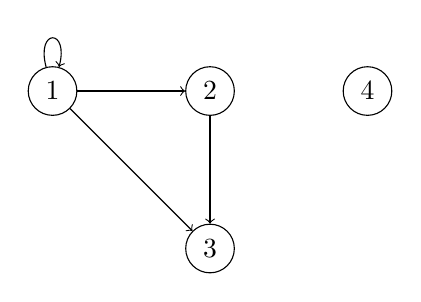
\begin{tikzpicture}[->,node distance=2cm]
  \node[draw,circle] (A) {$1$};
  \node[draw,circle] (B) [right of=A] {$2$};
  \node[draw,circle] (C) [below of=B] {$3$};
  \node[draw,circle] (D) [right of=B] {$4$};
  \draw (A) to [loop above]  (A);
  \draw (A) to  (B);
  \draw (A) to  (C);
  \draw (B) to  (C);
  \end{tikzpicture}
\intertext{આ આલેખ $\tuple{V', E}$થી જુદો છે,
  જેમાં $V' = \{1, 2, 3\}$ છે અને જે આવો દેખાય છે:}
& 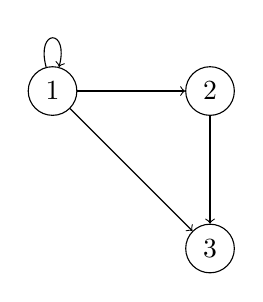
\begin{tikzpicture}[->,node distance=2cm]
  \node[draw,circle] (A) {$1$};
  \node[draw,circle] (B) [right of=A] {$2$};
  \node[draw,circle] (C) [below of=B] {$3$};
  \draw (A) to [loop above]  (A);
  \draw (A) to  (B);
  \draw (A) to  (C);
  \draw (B) to  (C);
  \end{tikzpicture}
\end{align*}
\end{ex}

\begin{prob}
  ગણ $\{1, 2, 3, 4\}$ પરના કરતાં-નાનું-અથવા-સમાન
  સંબંધ $\le$ને આલેખ તરીકે લો અને તેને અનુરૂપ આકૃતિ દોરો.
\end{prob}




\olfileid{sfr}{rel}{tre}
\olsection{વૃક્ષો}

તર્કશાસ્ત્રના બધા ભાગોમાં મહત્વનો ભાગ ભજવતો આંશિક ક્રમનો
એક ખાસ પ્રકાર \emph{વૃક્ષ} છે. તર્કશાસ્ત્રના પ્રાથમિક ભાગોમાં
સાંત વૃક્ષો આવે છે: દાખલા તરીકે, સૂત્રોને વાક્યરચના
વૃક્ષમાં તેમના વિઘટન દ્વારા સમજી શકાય છે, જ્યારે ઘણી
નિષ્પત્તિ પદ્ધતિઓમાં નિષ્પત્તિઓ પણ સાંત વૃક્ષોનું
રૂપ ધરાવે છે.
%
વિધાનાત્મક અને પ્રથમ ક્રમના તર્કશાસ્ત્ર માટેના પૂર્ણતા પ્રમેયોની
સાબિતીમાં જ અનંત વૃક્ષો દેખાય છે, અને ગાણિતિક તર્કશાસ્ત્રમાં
સર્વત્ર તેમનો ઉપયોગ થાય છે.

ગણસિદ્ધાંતમાં વૃક્ષનો ખ્યાલ, આલેખસિદ્ધાંતમાં વૃક્ષના ખ્યાલ સાથે
ગાઢ રીતે જોડાયેલો છે. અહીં એક (સાંત) વૃક્ષનું ચિત્ર છે:

\begin{center}
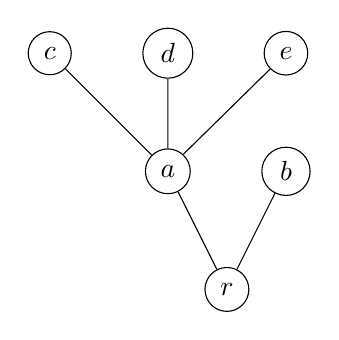
\begin{tikzpicture}[nodes={draw, circle}, -]
\node{$r$} [grow'=up]
    child { node {$a$}
        child { node {$c$} }
        child { node {$d$} }
        child { node {$e$} }
    }
    child { node {$b$} };
\end{tikzpicture}
\end{center}

સૌથી નીચેની ગાંઠ $r$ મૂળ છે. $r$ સિવાયની દરેક ગાંઠની
તરત નીચે બરાબર એક જનક ગાંઠ છે.
ગાંઠ $x$થી ધારોને અનુસરીને ઉપર જતાં ગાંઠ $y$ સુધી પહોંચી
શકાય ત્યારે $x$નો $y$ સાથેનો સંબંધ,
$x$ એ $y$નો \emph{પૂર્વજ} છે એમ સમજી શકાય.

વૃક્ષમાં પૂર્વજનો સંબંધ કડક આંશિક ક્રમ છે.
આ પરથી ગણસિદ્ધાંતની વ્યાખ્યા આપવાની પ્રેરણા મળે છે.
તે રજૂ કરવા માટે આપણને બે ખ્યાલો જોઈએ.
$\le$ વડે આંશિક ક્રમમાં ગોઠવેલા ગણ $A$માં
\emph{લઘુતમ ઘટક} એવો ઘટક $x \in A$ છે
કે દરેક $y \in A$ માટે $x \le y$.
ગણ $\le$ વડે \emph{સુક્રમિત} હોય જો તેના દરેક
અરિક્ત ઉપગણમાં લઘુતમ ઘટક હોય.

\begin{defn}[વૃક્ષ]
\emph{વૃક્ષ} એવો જોડ $T = \tuple{A, \le}$ છે કે $A$ એક ગણ છે
અને $\le$ એ $A$ પરનો આંશિક ક્રમ છે, જેમાં એકમાત્ર લઘુતમ
ઘટક $r \in A$ છે (જેને \emph{મૂળ} કહે છે), અને
દરેક $x \in A$ માટે ગણ $\Setabs{y}{y \le x}$
એ $\le$ વડે સુક્રમિત છે.
\end{defn}

\begin{defn}[અનુગામીઓ]
ધારો કે $T = \tuple{A, \le}$ વૃક્ષ છે.
જો $x,y \in A$, $x < y$, અને $x < z < y$
થાય એવો કોઈ $z \in A$ ન હોય, તો આપણે કહીએ છીએ કે
$y$ એ $x$નો \emph{અનુગામી} છે.
\end{defn}

$x \in A$ના અનુગામીઓને તેની \emph{સંતાન ગાંઠો} પણ કહે છે.
જો $y$ એ $x$નો અનુગામી હોય, તો આપણે $x$ને $y$નો
\emph{પુરોગામી} અથવા \emph{જનક} કહીએ છીએ.

\begin{prop}
જો $\tuple{A,\le}$ વૃક્ષ હોય, તો મૂળ સિવાયના
દરેક $x \in A$નો વધુમાં વધુ એક પુરોગામી હોય.
\end{prop}

\begin{proof}
  ધારો કે $y_1 < x$ અને $y_2 < x$ અને $y_1 \neq y_2$.
  તો $\{y_1, y_2\} \subseteq \Setabs{z}{z<x}$.
  $\Setabs{z}{z<x}$ એ $\le$ વડે સુક્રમિત હોવાથી,
  તેના ઉપગણ $\{y_1, y_2\}$માં લઘુતમ ઘટક છે,
  જે દેખીતી રીતે કાં $y_1$ અથવા $y_2$ હોવો જોઈએ.
  તેથી કાં $y_1 \le y_2$ અથવા $y_2 \le y_1$.
  આપણે $y_1 \neq y_2$ ધાર્યું હતું, તેથી ખરેખર
  કાં $y_1 < y_2$ અથવા $y_2 < y_1$.
  આપણે $y_1 < x$ અને $y_2 < x$ ધાર્યું હોવાથી,
  વધુમાં કાં $y_1 < y_2 < x$ અથવા $y_2 < y_1 < x$.
  તેથી $y_1$ અને $y_2$ બંને $x$ના પુરોગામી હોઈ શકે નહીં.
\end{proof}

\begin{defn}
વૃક્ષ $T = \tuple{A, \le}$ \emph{અનંત} કહેવાય જો $A$
અનંત ગણ હોય, અને નહિતર \emph{સાંત} કહેવાય.
જો $T$માં દરેક $x \in A$ના માત્ર સાંત સંખ્યામાં અનુગામીઓ હોય,
તો આપણે કહીએ છીએ કે $T$ \emph{સાંત શાખનવાળું} છે.
\end{defn}

\begin{defn}[શાખાઓ]
વૃક્ષ $T = \tuple{A, \le}$ આપેલું હોય ત્યારે,
$T$ની \emph{શાખા} એ $T$માં સમાવેશની દૃષ્ટિએ મહત્તમ શૃંખલા છે,
એટલે કે, એવો ગણ $B \subseteq A$ કે કોઈ પણ
$x, y \in B$ માટે કાં $x \le y$ અથવા $y \le x$,
અને કોઈ પણ $z \in X \setminus B$ માટે એવો
$u \in B$ અસ્તિત્વ ધરાવે છે કે ન તો $z \le u$, ન તો $u \le z$.
%
આપણે $T$ની બધી શાખાઓના ગણને દર્શાવવા $[T]$ વાપરીએ છીએ.
\end{defn}

\begin{ex}
સાંત શાખનવાળા વૃક્ષનું એક સુપ્રસિદ્ધ ઉદાહરણ એ $0$ અને $1$ના
સાંત અનુક્રમોનું \emph{અનંત દ્વિઆધારી વૃક્ષ} છે,
જેને ક્યારેક $\{0,1\}^*$ અથવા $\Bin^*$થી દર્શાવવામાં આવે છે,
અને જે વિસ્તરણ સંબંધ $\sqsubseteq$ વડે ક્રમિત છે
(દા.ત., $101 \sqsubseteq 101101$).
કોઈ પણ દ્વિઆધારી પ્રતીકશ્રેણીને અંતે $0$ કે $1$ ઉમેરીને
હંમેશાં વિસ્તારી શકાય છે, તેથી આ વૃક્ષમાં અનંત સંખ્યામાં
ઘટકો છે: દરેક ઘટક $s$ના બરાબર બે અનુગામી $s0$ અને $s1$ છે.
તેનું મૂળ ખાલી અનુક્રમ $\emptyseq$ છે.
\end{ex}

\begin{ex}
થોડું વધુ સામાન્ય રીતે, વિસ્તરણ સંબંધ $\sqsubseteq$ સાથે
પ્રાકૃતિક સંખ્યાઓના સાંત અનુક્રમોનો ગણ $\Nat^*$ પણ વૃક્ષ છે.
તે દેખીતી રીતે સાંત શાખનવાળું નથી: દરેક $s \in \Nat^*$ના
અનંત સંખ્યામાં અનુગામી $sn$ છે, દરેક $n \in \Nat$ માટે એક.
$\sqsubseteq$ હેઠળ સંવૃત એવો દરેક $A \subseteq \Nat^*$
એ $\Nat^*$નું \emph{ઉપવૃક્ષ} છે.
(એટલે કે, $A$ એવો છે કે જો $s \in A$ અને
$s' \sqsubseteq s$, તો $s' \in A$ પણ.)
બધાં સાંત વૃક્ષોને $\Nat^*$નાં સાંત ઉપવૃક્ષો તરીકે રજૂ કરી શકાય છે.
\end{ex}

\begin{prop}[કેનિગનું સહાયક પ્રમેય]
જો $T = \tuple{A,\le}$ સાંત શાખનવાળું અનંત વૃક્ષ હોય,
તો $T$ને અનંત શાખા હોય છે.
\end{prop}

સંગણનીયતાના સિદ્ધાંતમાં વ્યાપકપણે વપરાતો કેનિગના સહાયક
પ્રમેયનો એક વિશેષ કિસ્સો, જેને \emph{નબળું કેનિગ સહાયક પ્રમેય}
કહે છે, આ છે: $\{0,1\}^*$ના કોઈ પણ અનંત ઉપવૃક્ષને
અનંત શાખા હોય છે.




\olfileid{sfr}{rel}{ops}
\olsection{સંબંધો પરની ક્રિયાઓ}

સંબંધોમાં ફેરફાર કરવો અથવા તેમને ભેગા કરવા ઘણી વાર ઉપયોગી
બને છે. \olref[sfr][rel][ord]{prop:stricttopartial}માં આપણે
સંબંધોના \emph{યોગગણ}નો વિચાર કર્યો હતો, જે બે સંબંધોને
જોડના ગણ તરીકે લઈએ ત્યારે તેમનો યોગગણ જ છે.
એ જ રીતે, \olref[sfr][rel][ord]{prop:partialtostrict}માં
આપણે સંબંધોના સાપેક્ષ તફાવતનો વિચાર કર્યો હતો.
અહીં સંબંધો પર કરી શકાય તેવી કેટલીક બીજી ક્રિયાઓ આપેલી છે.

\begin{defn}\ollabel{relationoperations}
ધારો કે $R$, $S$ સંબંધો છે, અને $A$ કોઈ પણ ગણ છે.

$R$નો \emph{વ્યસ્ત} એ
$R^{-1} = \Setabs{\tuple{y, x}}{\tuple{x, y} \in R}$ છે.

$R$ અને $S$નો \emph{સાપેક્ષ ગુણાકાર} એ
$(R \mid S) = \{\tuple{x, z} : \exists y(Rxy \land Syz)\}$ છે.

$R$નું $A$ પર \emph{મર્યાદન} એ
$\funrestrictionto{R}{A}= R \cap A^2$ છે.

$R$ને $A$ પર \emph{લાગુ પાડતાં મળતો ગણ} એ
$\funimage{R}{A} = \{y : (\exists x \in A)Rxy\}$ છે.
\end{defn}

\begin{ex}
ધારો કે $S \subseteq \Int^2$ એ $\Int$ પરનો અનુગામી સંબંધ છે,
એટલે કે $S = \Setabs{\tuple{x, y} \in \Int^2}{x + 1 = y}$,
જેથી $Sxy$ તો અને તો જ $x + 1 = y$.

$S^{-1}$ એ $\Int$ પરનો પુરોગામી સંબંધ છે,
એટલે કે $\Setabs{\tuple{x,y}\in\Int^2}{x -1 =y}$.

$S\mid S$ એ
$ \Setabs{\tuple{x,y}\in\Int^2}{x + 2 =y}$ છે.

$\funrestrictionto{S}{\Nat}$ એ $\Nat$ પરનો અનુગામી સંબંધ છે.

$\funimage{S}{\{1,2,3\}}$ એ $\{2, 3, 4\}$ છે.
\end{ex}

\begin{defn}[પરંપરિત સંવરણ]ધારો કે $R \subseteq A^2$ દ્વિઘટકી સંબંધ છે.

$R$નું \emph{પરંપરિત સંવરણ} એ
$R^+ = \bigcup_{0 < n \in \Nat} R^n$ છે,
જ્યાં આપણે પુનરાવર્તી રીતે $R^1 = R$ અને
$R^{n+1} = R^n \mid R$ વ્યાખ્યાયિત કરીએ છીએ.

$R$નું \emph{સ્વવાચક પરંપરિત સંવરણ} એ
$R^* = R^+ \cup \Id{A}$ છે.
\end{defn}

\begin{ex}
અનુગામી સંબંધ $S \subseteq \Int^2$ લો.
$S^2xy$ તો અને તો જ $x + 2 = y$,
$S^3xy$ તો અને તો જ $x + 3 = y$, વગેરે.
તેથી $S^+xy$ તો અને તો જ કોઈક $n \geq 1$ માટે
$x + n = y$. બીજા શબ્દોમાં, $S^+xy$ તો અને તો જ $x < y$,
અને $S^*xy$ તો અને તો જ $x \le y$.
\end{ex}

\begin{prob}
$R$નું પરંપરિત સંવરણ ખરેખર પરંપરિત છે તે દર્શાવો.
\end{prob}


\part{વિધેયો}


\olfileid{sfr}{fun}{bas}
\olsection{પાયાની બાબતો}

\begin{explain}
\emph{વિધેય} એવું નિરૂપણ છે જે આપેલા ગણના દરેક ઘટકને
કોઈ (બીજા) આપેલા ગણના ચોક્કસ ઘટક પર મોકલે છે.
દાખલા તરીકે, $1$~ઉમેરવાની ક્રિયા એક વિધેય વ્યાખ્યાયિત કરે છે:
દરેક સંખ્યા~$n$નું નિરૂપણ અનન્ય સંખ્યા~$n+1$ પર થાય છે.

વધુ સામાન્ય રીતે, વિધેયો આગત તરીકે જોડ, ત્રિજોડ વગેરે લઈ
કોઈ પ્રકારનું નિર્ગત આપી શકે છે. પાયાના અંકગણિતમાંથી આપણને
ઘણાં વિધેયો પરિચિત છે. દાખલા તરીકે, સરવાળો અને ગુણાકાર
વિધેયો છે. તેઓ બે સંખ્યાઓ લે છે અને ત્રીજી સંખ્યા આપે છે.

આ ગાણિતિક, અમૂર્ત અર્થમાં વિધેય એક \emph{કાળી પેટી} છે:
કયા આગત સાથે કયું નિર્ગત જોડાયેલું છે એટલું જ મહત્ત્વનું છે,
નિર્ગતની ગણતરી કરવાની પદ્ધતિ નહીં.
\end{explain}

\begin{defn}[વિધેય]
\emph{વિધેય} $f \colon A \to B$ એ $A$ના દરેક ઘટકનું
$B$ના કોઈ ઘટક પરનું નિરૂપણ છે.

આપણે $A$ને $f$નો \emph{પ્રદેશ} અને $B$ને $f$નો
\emph{સહપ્રદેશ} કહીએ છીએ. $A$ના ઘટકોને $f$નાં
આગતો અથવા \emph{દલીલો} કહે છે; અને $f$ દ્વારા દલીલ~$x$ સાથે
જોડાતા $B$ના ઘટકને દલીલ~$x$ માટેની
\emph{$f$ની કિંમત} કહે છે, જેને $f(x)$ લખાય છે.

$f$નો \emph{વિસ્તાર} $\ran{f}$ એ સહપ્રદેશનો એવો ઉપગણ છે
જેમાં કોઈક દલીલ માટેની $f$ની કિંમતો આવે છે;
$\ran{f} =
\Setabs{f(x)}{x \in A}$.
\end{defn}

\olref{fig:function}માંનું ચિત્ર વિધેયો વિશે વિચારવામાં મદદરૂપ
થઈ શકે છે. ડાબી બાજુનો લંબવૃત્ત વિધેયનો \emph{પ્રદેશ}
દર્શાવે છે; જમણી બાજુનો લંબવૃત્ત તેનો \emph{સહપ્રદેશ}
દર્શાવે છે; અને તીર પ્રદેશની \emph{દલીલ}થી સહપ્રદેશની
તેને અનુરૂપ \emph{કિંમત} તરફ જાય છે.

\begin{figure}
  \olasset{assets/diagrams/function.tikz}
  \caption{વિધેય એ એક ગણના દરેક ઘટકનું બીજા ગણના
    ઘટક પરનું નિરૂપણ છે. તીર પ્રદેશની દલીલથી
    સહપ્રદેશની તેને અનુરૂપ કિંમત તરફ જાય છે.}
  \ollabel{fig:function}
\end{figure}

\begin{ex}
ગુણાકાર પ્રાકૃતિક સંખ્યાઓની જોડને આગત તરીકે લે છે અને
પ્રાકૃતિક સંખ્યાઓને નિર્ગત તરીકે આપે છે. તેથી તે
$\Nat \times \Nat$ (પ્રદેશ)થી $\Nat$ (સહપ્રદેશ)માં જાય છે.
તેનો વિસ્તાર પણ $\Nat$ છે, કારણ કે દરેક $n \in \Nat$
એ $n \times 1$ છે.
\end{ex}

\begin{ex}
ગુણાકાર વિધેય છે, કારણ કે તે દરેક આગતને---પ્રાકૃતિક સંખ્યાઓની
દરેક જોડને---એક જ નિર્ગત સાથે જોડે છે:
$\times \colon \Nat^2 \to
\Nat$. તેનાથી વિપરીત, પ્રાકૃતિક સંખ્યા~$n$ને
$x^2 = n$ થાય એવી વાસ્તવિક સંખ્યા~$x$ પર મોકલતું નિરૂપણ
વિધેયાત્મક નથી, કારણ કે દરેક ધન પૂર્ણાંક~$n$નાં બે વર્ગમૂળ
છે: $\sqrt{n}$ અને~$-\sqrt{n}$. માત્ર અનૃણ (મુખ્ય) વર્ગમૂળ આપીને
આ નિરૂપણને વિધેયાત્મક બનાવી શકીએ:
$\sqrt{\phantom{X}} \colon
\Nat \to \Real$.
\end{ex}
\sourcecorrection{OLFUN-002}{મૂળની \texttt{function-basics.tex}, પંક્તિઓ
64--71માં પ્રદેશમાં શૂન્યનો સમાવેશ હોવા છતાં ``ધન વર્ગમૂળ'' કહેવાયું છે.
અહીં શૂન્યને પણ આવરી લેતું ``અનૃણ (મુખ્ય) વર્ગમૂળ'' લખ્યું છે.}

\begin{ex}
વર્ગના દરેક વિદ્યાર્થીને તેના અંતિમ ગુણાંક સાથે જોડતો સંબંધ
વિધેય છે---એક જ વર્ગમાં કોઈ વિદ્યાર્થીને બે જુદા અંતિમ
ગુણાંક મળી શકે નહીં. વર્ગના દરેક વિદ્યાર્થીને તેનાં
માતાપિતા સાથે જોડતો સંબંધ વિધેય નથી: વિદ્યાર્થીઓને
શૂન્ય, બે કે વધુ માતાપિતા હોઈ શકે છે.
\end{ex}

\begin{explain}
દરેક સંભવિત દલીલ માટે વિધેયની કિંમત શું છે તે કોઈ ચોક્કસ
રીતે જણાવીને આપણે વિધેયો વ્યાખ્યાયિત કરી શકીએ છીએ.
તે માટે સૂત્ર આપી શકાય, કિંમતની ગણતરી કરવાની પદ્ધતિ
વર્ણવી શકાય, અથવા દરેક દલીલની કિંમતોની યાદી આપી શકાય.
વિધેયને ગમે તે રીતે વ્યાખ્યાયિત કરીએ, દરેક દલીલ માટે
એક અને માત્ર એક કિંમત નક્કી કરી છે તેની ખાતરી કરવી જોઈએ.
\end{explain}

\begin{ex}
$f(x) = x+1$ થાય તે રીતે $f \colon \Nat \to \Nat$
વ્યાખ્યાયિત કરીએ. આ વ્યાખ્યા $f$ને એવું વિધેય બનાવે છે
જે પ્રાકૃતિક સંખ્યાઓ લે છે અને પ્રાકૃતિક સંખ્યાઓ આપે છે.
તે જણાવે છે કે પ્રાકૃતિક સંખ્યા~$x$ આપતાં $f$ તેનું
અનુગામી~$x+1$ આપશે.
આ કિસ્સામાં સહપ્રદેશ $\Nat$ એ $f$નો વિસ્તાર નથી,
કારણ કે પ્રાકૃતિક સંખ્યા~$0$ કોઈ પ્રાકૃતિક સંખ્યાનું
અનુગામી નથી. $f$નો વિસ્તાર બધા ધન પૂર્ણાંકોનો ગણ
$\Int^{+}$ છે.
\end{ex}

\begin{ex}\ollabel{examplefunext}
$g(x) = x+2-1$ થાય તે રીતે $g \colon \Nat \to \Nat$
વ્યાખ્યાયિત કરીએ. આ જણાવે છે કે $g$ પ્રાકૃતિક સંખ્યાઓ
લેતું અને પ્રાકૃતિક સંખ્યાઓ આપતું વિધેય છે.
પ્રાકૃતિક સંખ્યા~$x$ આપતાં $g$, $x$ના અનુગામીના
અનુગામીનો પુરોગામી, એટલે કે $x+1$, આપશે.
\end{ex}
\sourcecorrection{OLFUN-003}{મૂળની \texttt{function-basics.tex}, પંક્તિઓ
103--107માં આગતનું નામ પહેલાં \(n\) અને પછી \(x\) છે. વ્યાખ્યા અને
પછીના સૂત્ર સાથે સુસંગત રહે તે માટે અહીં સર્વત્ર \(x\) વાપર્યું છે.}

\begin{explain}
આપણે હમણાં જુદી \emph{વ્યાખ્યાઓ} ધરાવતા બે વિધેયો,
$f$ અને $g$, જોયાં. જોકે, આ \emph{એક જ વિધેય} છે.
કારણ કે કોઈ પણ પ્રાકૃતિક સંખ્યા~$n$ માટે
$f(n) = n+1 = n+2-1 =
g(n)$ થાય છે. બીજા શબ્દોમાં, $f$ અને~$g$ માટેની આપણી
વ્યાખ્યાઓ જુદાં સમીકરણો દ્વારા એક જ નિરૂપણ નક્કી કરે છે.
આમ, ગર્ભિત રીતે આપણે વિધેયો માટે દલીલોની કિંમતો દ્વારા
નિર્ધારિત સમાનતાના સિદ્ધાંત પર આધાર રાખીએ છીએ:
\[
  \text{જો }\forall x\, f(x) = g(x)\text{, તો }f = g
\]
શરત એટલી કે $f$ અને~$g$નો પ્રદેશ અને સહપ્રદેશ એક જ હોય.
\end{explain}

\begin{ex}
આપણે કિસ્સા પાડી વિધેયો વ્યાખ્યાયિત પણ કરી શકીએ.
દાખલા તરીકે, $h \colon \Nat \to \Nat$ને આમ વ્યાખ્યાયિત
કરી શકીએ:
\[
h(x) =
\begin{cases}
  \frac{x}{2} & \text{જો $x$ યુગ્મ હોય} \\
  \frac{x+1}{2} & \text{જો $x$ અયુગ્મ હોય.}
\end{cases}
\]
દરેક પ્રાકૃતિક સંખ્યા યુગ્મ કે અયુગ્મ હોવાથી, આ વિધેયનું
નિર્ગત હંમેશાં પ્રાકૃતિક સંખ્યા હશે. એટલું યાદ રાખો કે
કિસ્સા પાડી વિધેય વ્યાખ્યાયિત કરો ત્યારે દરેક સંભવિત
આગત ચોક્કસ એક કિસ્સામાં આવવું જોઈએ. કેટલીક વાર
કિસ્સાઓ બધા આગતોને આવરી લે છે અને પરસ્પર અલગ છે
તે સાબિત કરવું જરૂરી બનશે.
\end{ex}




\olfileid{sfr}{fun}{kin}
\olsection{વિધેયોના પ્રકારો}

\begin{explain}
આપણને વારંવાર મળતા વિધેયોના કેટલાક પ્રકારોનું
વર્ગીકરણ રજૂ કરવું ઉપયોગી થશે.

શરૂઆતમાં એવાં વિધેયો લઈએ જેમના સહપ્રદેશનો દરેક સભ્ય
વિધેયની કિંમત હોય. આવાં વિધેયોને વ્યાપ્ત કહે છે;
તેમને \olref{fig:surjective} પ્રમાણે ચિત્રમાં દર્શાવી શકાય.

\begin{figure}
  \olasset{assets/diagrams/surjective.tikz}
  \caption{વ્યાપ્ત વિધેયના સહપ્રદેશનો દરેક
    ઘટક તેની કિંમત હોય છે.}
  \ollabel{fig:surjective}
\end{figure}
\end{explain}

\begin{defn}[વ્યાપ્ત વિધેય]
વિધેય $f \colon A \rightarrow B$ \emph{વ્યાપ્ત}
હોય જો અને માત્ર જો $B$ એ $f$નો વિસ્તાર પણ હોય, એટલે કે
દરેક $y \in B$ માટે ઓછામાં ઓછો એક $x \in A$
એવો હોય કે $f(x) = y$; અથવા પ્રતીકોમાં:
\[
  (\forall y \in B)(\exists x \in A)f(x) = y.
\]
આવા વિધેયને $A$થી $B$માંનું વ્યાપ્ત વિધેય કહીએ છીએ.
\end{defn}

\begin{explain}
$f$ એ વ્યાપ્ત વિધેય છે તે બતાવવા, તમારે બતાવવું પડે
કે $f$ના સહપ્રદેશની દરેક વસ્તુ કોઈક આગત $x$ માટે
$f(x)$ની કિંમત છે.

નોંધો કે કોઈ પણ વિધેય વ્યાપ્ત વિધેય
\emph{ઉત્પન્ન કરે છે}. કારણ કે આપેલા વિધેય
$f \colon A \to B$ માટે $f'(x) = f(x)$ દ્વારા
$f' \colon A \to \ran{f}$ વ્યાખ્યાયિત કરીએ.
$\ran{f}$ની \emph{વ્યાખ્યા} જ
$\Setabs{f(x) \in B}{x \in A}$ હોવાથી આ વિધેય
$f'$ ચોક્કસ વ્યાપ્ત વિધેય છે.
\end{explain}

\begin{explain}
કોઈ પણ વિધેય દરેક સંભવિત આગતને અનન્ય નિર્ગત પર મોકલે છે.
પરંતુ એવાં વિધેયો પણ છે જે જુદાં આગતોને કદી એક જ
નિર્ગત પર મોકલતાં નથી. આવાં વિધેયોને એક-એક
કહે છે; તેમને \olref{fig:injective} પ્રમાણે ચિત્રમાં
દર્શાવી શકાય.
\begin{figure}
  \olasset{assets/diagrams/injective.tikz}
  \caption{એક-એક વિધેય કદી બે જુદી દલીલોને
    એક જ કિંમત પર મોકલતું નથી.}
  \ollabel{fig:injective}
\end{figure}
\end{explain}

\begin{defn}[એક-એક વિધેય]
વિધેય $f \colon A \rightarrow B$ \emph{એક-એક}
હોય જો અને માત્ર જો દરેક $y \in B$ માટે વધુમાં વધુ
એક $x \in A$ એવો હોય કે $f(x) = y$.
આવા વિધેયને $A$થી $B$માંનું એક-એક વિધેય કહીએ છીએ.
\end{defn}

\begin{explain}
$f$ એ એક-એક વિધેય છે તે બતાવવા, તમારે બતાવવું પડે
કે $f$ના પ્રદેશના કોઈ પણ ઘટકો $x$ અને $y$
માટે, જો $f(x)=f(y)$ હોય, તો $x=y$ થાય છે.
\end{explain}

\begin{ex}
$f(x) = 1$ દ્વારા આપેલું અચળ વિધેય
$f\colon \Nat \to \Nat$ એક-એક પણ નથી
અને વ્યાપ્ત પણ નથી.

$f(x) = x$ દ્વારા આપેલું તદેવ વિધેય
$f\colon \Nat \to \Nat$ એક-એક અને
વ્યાપ્ત બંને છે.

$f(x) = x+1$ દ્વારા આપેલું અનુગામી વિધેય
$f \colon \Nat \to \Nat$ એક-એક છે,
પરંતુ વ્યાપ્ત નથી.

નીચે મુજબ વ્યાખ્યાયિત વિધેય $f \colon \Nat \to \Nat$:
\[
  f(x) =
  \begin{cases}
    \frac{x}{2} & \text{જો $x$ યુગ્મ હોય} \\
    \frac{x+1}{2} & \text{જો $x$ અયુગ્મ હોય.}
  \end{cases}
\]
વ્યાપ્ત છે, પરંતુ એક-એક નથી.
\end{ex}

\begin{explain}
ઘણી વાર આપણે એક-એક અને વ્યાપ્ત બંને
હોય એવાં વિધેયો લેવા માગીએ છીએ. આવાં વિધેયોને
એક-એક અને વ્યાપ્ત કહીએ છીએ. તેઓ
\olref{fig:bijective}માં દર્શાવેલા વિધેય જેવાં દેખાય છે.
એક-એક વ્યાપ્ત વિધેયોને ક્યારેક \emph{પરસ્પર એક-એક સંગતતાઓ}
પણ કહે છે, કારણ કે તેઓ સહપ્રદેશના ઘટકોને પ્રદેશના
ઘટકો સાથે અનન્ય રીતે જોડે છે.
\begin{figure}
  \olasset{assets/diagrams/bijective.tikz}
  \caption{એક-એક અને વ્યાપ્ત વિધેય સહપ્રદેશના ઘટકોને
    પ્રદેશના ઘટકો સાથે અનન્ય રીતે જોડે છે.}
  \ollabel{fig:bijective}
\end{figure}
\end{explain}

\begin{defn}[એક-એક વ્યાપ્ત વિધેય]
વિધેય $f \colon A \to B$ \emph{એક-એક અને વ્યાપ્ત} હોય
જો અને માત્ર જો તે વ્યાપ્ત અને એક-એક
બંને હોય. આવા વિધેયને $A$થી $B$માંનું
(અથવા $A$ અને~$B$ વચ્ચેનું) એક-એક વ્યાપ્ત વિધેય કહીએ છીએ.
\end{defn}




\olfileid{sfr}{fun}{rel}

\olsection{સંબંધો તરીકે વિધેયો}

\begin{explain}
$A$ના ઘટકોને $B$ના ઘટકો પર મોકલતું
વિધેય સ્પષ્ટપણે $A$ અને~$B$ વચ્ચે સંબંધ વ્યાખ્યાયિત
કરે છે: $x$ અને $y$ વચ્ચે આ સંબંધ હોય જો અને માત્ર જો
$f(x) = y$ હોય. હકીકતમાં, દાખલા તરીકે ગણિતના પાયાના
ઘટકોની સંખ્યા ઘટાડવામાં રસ હોય તો, આપણે વિધેય~$f$ને
આ સંબંધ સાથે, એટલે કે જોડોના ગણ સાથે, \emph{એકરૂપ}
પણ ગણી શકીએ. ત્યારે પ્રશ્ન ઊભો થાય છે: કયા સંબંધો
આ રીતે વિધેયો વ્યાખ્યાયિત કરે છે?
\end{explain}

\begin{defn}[વિધેયનો આલેખ] ધારો કે $f\colon A \to B$
વિધેય છે. $f$નો \emph{આલેખ} એ નીચે પ્રમાણે વ્યાખ્યાયિત
સંબંધ $R_f \subseteq A \times B$ છે:
\[
R_f = \Setabs{\tuple{x,y}}{f(x) = y}.
\]
\end{defn}

\begin{explain}
ઘટકો દ્વારા નિર્ધારિત સમાનતાના સિદ્ધાંતથી વિધેયનો
આલેખ અનન્ય રીતે નક્કી થાય છે. વધુમાં, ગણો માટેનો
આ સિદ્ધાંત વિધેયો માટેના ગર્ભિત સમાનતાના સિદ્ધાંતને
તરત સમર્થન આપે છે: જો $f$ અને~$g$નો પ્રદેશ અને
સહપ્રદેશ એક જ હોય, તો બધી દલીલો માટેની કિંમતો
સરખી હોય ત્યારે તેઓ એક જ વિધેય હોય છે.

એ જ રીતે, સંબંધ “વિધેયાત્મક” હોય, તો તે કોઈ
વિધેયનો આલેખ છે.
\end{explain}

\begin{prop}\ollabel{prop:graph-function}
ધારો કે $R \subseteq A \times B$ એવો છે કે:
\begin{enumerate}
\item જો $Rxy$ અને $Rxz$ હોય, તો $y = z$; અને
\item દરેક $x \in A$ માટે કોઈક $y \in B$ એવો છે
કે $\tuple{x,
y} \in R$.
\end{enumerate}
તો $R$ એ $f(x) = y$ જો અને માત્ર જો $Rxy$
દ્વારા વ્યાખ્યાયિત વિધેય $f\colon A \to B$નો આલેખ છે.
\end{prop}

\begin{proof}
ધારો કે $Rxy$ થાય એવો $y$ છે. જો $Rxz$ થાય એવો
બીજો $z \neq
y$ હોત, તો $R$ પરની શરતનો ભંગ થાત.
આથી, $Rxy$ થાય એવો $y$ હોય, તો આ $y$ અનન્ય છે,
અને તેથી $f$ સુવ્યાખ્યાયિત છે. સ્પષ્ટપણે $R_f = R$.
\end{proof}

\begin{explain}
દરેક વિધેય $f\colon A \to B$નો આલેખ હોય છે, એટલે કે
$f(x) = y$ દ્વારા વ્યાખ્યાયિત $A
\times B$માં સમાયેલો સંબંધ. બીજી તરફ,
\olref{prop:graph-function}માં આપેલા ગુણધર્મો ધરાવતો
દરેક સંબંધ~$R
\subseteq A \times B$ કોઈ વિધેય~$f \colon A \to
B$નો આલેખ છે. વિધેયો અને તેમના આલેખો વચ્ચેના આ ગાઢ
સંબંધને કારણે આપણે વિધેયને તેના આલેખ તરીકે જ વિચારી શકીએ.
બીજા શબ્દોમાં, વિધેયોને અમુક સંબંધો સાથે, એટલે કે અમુક
બહુજોડોના ગણો સાથે, એકરૂપ ગણી શકાય.
\oliflabeldef{sfr:rel:ref:sec}{જોકે, નોંધો કે આ “એકરૂપતા”નો
આશય \olref[sfr][rel][ref]{sec}માં જણાવ્યો હતો તેવો છે:
તે વિધેયોના તત્વમીમાંસાકીય સ્વરૂપ વિશેનો દાવો નથી;
વિધેયોને અમુક ગણો તરીકે \emph{લેવાં} અનુકૂળ છે એવી
નોંધ છે. આ અનુકૂળતાનું એક કારણ એ છે કે આપણે}{આપણે}
હવે સંબંધો પર કરેલી ક્રિયાઓ જેવી ક્રિયાઓ વિધેયો પર
કરવાનું વિચારી શકીએ છીએ (જુઓ \olref[sfr][rel][ops]{sec}).
ખાસ કરીને:
\end{explain}
\sourcecorrection{OLFUN-004}{મૂળની \texttt{functions-relations.tex}, પંક્તિઓ
60--68માં આલેખને ``\(A\times B\) પરનો સંબંધ'' કહેવાયો છે. પ્રોજેક્ટની
પોતાની વ્યાખ્યા પ્રમાણે અહીં \(A\) અને \(B\) વચ્ચેનો, એટલે કે
\(A\times B\)માં સમાયેલો સંબંધ અભિપ્રેત છે; અનુવાદમાં એ પ્રકાર સ્પષ્ટ કર્યો છે.}

\begin{defn}\ollabel{defn:funimage}
ધારો કે $f \colon A \to B$ વિધેય છે અને $C\subseteq A$ છે.

$f$નું $C$ પરનું \emph{મર્યાદન} એ બધા $x \in C$ માટે
$(\funrestrictionto{f}{C})(x) = f(x)$ દ્વારા વ્યાખ્યાયિત
વિધેય~$\funrestrictionto{f}{C}\colon C \to B$ છે.
બીજા શબ્દોમાં, $\funrestrictionto{f}{C} = \Setabs{\tuple{x, y} \in R_f}{x \in
C}$.

$C$ પર $f$નું \emph{પ્રયોજન} એ $\funimage{f}{C} =
\Setabs{f(x)}{x \in C}$ છે. તેને $f$ હેઠળનું
$C$નું \emph{પ્રતિબિંબ} પણ કહીએ છીએ.
\end{defn}

\begin{explain}
આ વ્યાખ્યાઓ પરથી કોઈ પણ વિધેય~$f$ માટે
$\ran{f} =
\funimage{f}{\dom{f}}$ મળે છે.
\oliflabeldef{sfr:rel:ops:sec}{\olref[sfr][rel][ops]{sec}ની
વ્યાખ્યાઓ અને વિધેયોને સંબંધો સાથે એકરૂપ ગણવાની આપણી
રીત જોતાં, આ ખ્યાલો અનુરૂપ છે. અહીં વિધેયનું મર્યાદન
માત્ર પ્રદેશને C સુધી સીમિત કરે છે; અગાઉનું સંબંધ-મર્યાદન
બંને અવયવોને C સુધી સીમિત કરે છે. પરંતુ બે બીજી
ક્રિયાઓ---વ્યસ્ત અને સાપેક્ષ ગુણાકાર---માટે થોડી વધુ
વિગત જરૂરી છે. તે \olref[inv]{sec} અને
\olref[cmp]{sec}માં આપીશું.}{}
\end{explain}
\sourcecorrection{OLFUN-005}{મૂળની \texttt{functions-relations.tex}, પંક્તિઓ
78--100માં વિધેય-મર્યાદનની સ્પષ્ટ વ્યાખ્યા સાચી છે, પરંતુ તેને અગાઉના
બંને-અવયવવાળા સંબંધ-મર્યાદન સાથે ``ચોક્કસ'' સરખું કહેવાયું છે. અહીં
આ સામ્યની મર્યાદા સ્પષ્ટ કરી છે.}




\olfileid{sfr}{fun}{inv}
\olsection{વિધેયોનાં પ્રતિવિધેયો}

\begin{explain}
આપણે વિધેયોને નિરૂપણો તરીકે વિચારીએ છીએ. તેથી વિધેયો
વિશે એક સ્વાભાવિક પ્રશ્ન એ છે કે નિરૂપણને “ઊલટાવી”
શકાય કે નહીં. દાખલા તરીકે, અનુગામી વિધેય
$f(x) = x + 1$ને આ અર્થમાં ઊલટાવી શકાય કે વિધેય
$g(y) = y - 1$ એ $f$ની ક્રિયાને “પાછી ફેરવે” છે.

પરંતુ સાવચેત રહેવું જોઈએ. $g$ની વ્યાખ્યા વિધેય
$\Int \to \Int$ વ્યાખ્યાયિત કરે છે, છતાં તે
\emph{વિધેય} $\Nat
\to \Nat$ વ્યાખ્યાયિત કરતી નથી, કારણ કે
$g(0) \notin \Nat$. એટલે સરળ કિસ્સામાં પણ વિધેયને
ઊલટાવી શકાય કે નહીં તે તરત સ્પષ્ટ થતું નથી;
તે પ્રદેશ અને સહપ્રદેશ પર આધાર રાખી શકે છે.

વિધેયના પ્રતિવિધેયનો ખ્યાલ આ વાતને વધુ ચોક્કસ બનાવે છે.
\end{explain}

\begin{defn}
વિધેય $g \colon B \to A$ એ વિધેય $f
\colon A \to B$નું \emph{પ્રતિવિધેય} છે જો બધા
$x \in A$ અને $y \in B$ માટે
$f(g(y)) = y$ અને $g(f(x)) = x$ થાય.
\end{defn}

જો $f$નું પ્રતિવિધેય~$g$ હોય, તો ઘણી વાર $g$ને
બદલે $f^{-1}$ લખીએ છીએ.

\begin{explain}
હવે વિધેયોને ક્યારે પ્રતિવિધેયો હોય છે તે નક્કી કરીશું.
$f\colon A \to B$ના પ્રતિવિધેય માટેનો યોગ્ય ઉમેદવાર
નીચે મુજબ “વ્યાખ્યાયિત” $g\colon B \to A$ છે:
\[
g(y) = \text{$f(x) = y$ થાય એવો “તે એક જ” $x$.}
\]
પરંતુ “વ્યાખ્યાયિત” (અને “તે એક જ”)ની આસપાસનાં
અવતરણચિહ્નો સૂચવે છે કે આ વ્યાખ્યા નથી. ઓછામાં ઓછું,
તે સંપૂર્ણ સામાન્યતાથી હંમેશાં કામ નહીં કરે. કારણ કે
આ વ્યાખ્યા વિધેય નક્કી કરે તે માટે $f(x) =
y$ થાય એવો એક અને માત્ર એક~$x$ હોવો જોઈએ---$g$નું
નિર્ગત અનન્ય રીતે નક્કી થવું જોઈએ. વધુમાં, દરેક
$y \in B$ માટે તે નક્કી થવું જોઈએ. જો $x_1$ અને
$x_2 \in
A$ એવા હોય કે $x_1 \neq x_2$ છતાં
$f(x_1) = f(x_2)$ હોય, તો $y = f(x_1) = f(x_2)$
માટે $g(y)$ અનન્ય રીતે નક્કી નહીં થાય. અને જો
$f(x) = y$ થાય એવો કોઈ~$x$ જ ન હોય, તો
$g(y)$ બિલકુલ નક્કી થતું નથી. બીજા શબ્દોમાં,
$g$ વ્યાખ્યાયિત થાય તે માટે $f$ એ એક-એક
અને વ્યાપ્ત બંને હોવું જોઈએ.

ધીમે ધીમે આગળ વધીએ. પ્રશ્નને બે ભાગમાં વહેંચીએ:
વિધેય~$f\colon A \to B$ આપેલું હોય ત્યારે
$g(f(x)) = x$ થાય એવું વિધેય $g\colon B \to A$
ક્યારે હોય? આવું $g$ એ $f$ની ક્રિયાને “પાછી ફેરવે” છે;
તેને $f$નો \emph{ડાબી બાજુનો વ્યસ્ત} કહે છે.
બીજું, $f(h(y)) = y$ થાય એવું વિધેય
$h\colon B \to A$ ક્યારે હોય? આવા $h$ને
$f$નો \emph{જમણી બાજુનો વ્યસ્ત} કહે છે---$f$
એ $h$ની ક્રિયાને “પાછી ફેરવે” છે.
\end{explain}

\begin{prop}
જો $f\colon A \to B$ એ એક-એક હોય અને તેનો પ્રદેશ અખાલી હોય, તો
$f$નો \emph{ડાબી બાજુનો વ્યસ્ત}~$g\colon B \to A$
હોય છે, જેથી બધા $x
\in A$ માટે $g(f(x)) = x$ થાય.
\end{prop}

\begin{proof}
ધારો કે $f\colon A \to B$ એ એક-એક છે અને તેનો પ્રદેશ અખાલી છે.
કોઈ $y \in B$ લો. જો $y \in \ran{f}$ હોય,
તો $f(x) = y$ થાય એવો $x \in A$ છે.
$f$ એ એક-એક હોવાથી આવો માત્ર એક~$x \in A$
છે. તેથી $g(y) = x$ વ્યાખ્યાયિત કરી શકીએ, એટલે કે
$g(y)$ એ $f(x)
= y$ થાય એવો “તે એક જ” $x \in A$ છે.
જો $y \notin \ran{f}$ હોય, તો તેને કોઈ પણ~$a \in A$
પર મોકલી શકીએ. એટલે એક $a \in A$ પસંદ કરી
$g\colon B \to A$ને આમ વ્યાખ્યાયિત કરી શકીએ:
\[
g(y) = \begin{cases}
    x & \text{જો $f(x) = y$ હોય}\\
    a & \text{જો $y \notin \ran{f}$ હોય.}
\end{cases}
\]
તે બધા $y \in B$ માટે વ્યાખ્યાયિત છે, કારણ કે
આવા દરેક $y \in \ran{f}$ માટે $f(x) = y$ થાય
એવો ચોક્કસ એક $x \in A$ છે. વ્યાખ્યા પ્રમાણે,
જો $y = f(x)$ હોય, તો $g(y) = x$ થાય,
એટલે કે $g(f(x)) = x$.
\end{proof}
\sourcecorrection{OLFUN-001}{મૂળની \texttt{inverses.tex}, પંક્તિઓ 62--84માં
પ્રદેશ અખાલી હોવાની શરત વિના આ વિધાન ખોટું છે: ખાલી ગણથી એક-ઘટકવાળા
ગણમાંનું ખાલી વિધેય એક-એક છે, પરંતુ તેનો ડાબી બાજુનો વ્યસ્ત નથી.
સરળ સુધારેલા વિધાનમાં પ્રદેશ અખાલી હોવાની શરત ઉમેરી છે. ચોક્કસ સામાન્ય
શરત એ છે કે પ્રદેશ અખાલી હોય અથવા સહપ્રદેશ ખાલી હોય.}

\begin{prob}
બતાવો કે જો $f\colon A \to B$નો ડાબી બાજુનો
વ્યસ્ત~$g$ હોય, તો $f$ એ એક-એક છે.
\end{prob}

\begin{prop}
જો $f\colon A \to B$ એ વ્યાપ્ત હોય, તો
$f$નો \emph{જમણી બાજુનો વ્યસ્ત}~$h\colon B \to A$
હોય છે, જેથી બધા~$y \in B$ માટે $f(h(y)) =
y$ થાય.
\end{prop}

\begin{proof}
ધારો કે $f\colon A \to B$ એ વ્યાપ્ત છે.
કોઈ $y \in
B$ લો. $f$ એ વ્યાપ્ત હોવાથી
$f(x_y)
= y$ થાય એવો $x_y \in A$ છે.
તેથી $h(y) = x_y$ વ્યાખ્યાયિત કરી શકીએ, એટલે કે
દરેક $y \in B$ માટે $f(x) = y$ થાય એવો કોઈ
$x \in A$ પસંદ કરીએ; $f$ એ વ્યાપ્ત
હોવાથી પસંદ કરવા માટે હંમેશાં ઓછામાં ઓછો એક હોય છે.
\footnote{$f$ એ વ્યાપ્ત હોવાથી દરેક~$y \in B$
માટે ગણ $\Setabs{x}{f(x) = y}$ ખાલી નથી.
$h$ની આપણી વ્યાખ્યા માટે આ દરેક ગણમાંથી એક જ $x$
પસંદ કરવો પડે છે. આ હંમેશાં શક્ય છે તે હકીકતમાં
સ્પષ્ટ નથી---આવી પસંદગીઓ કરવાની શક્યતા એક
સ્વયંસિદ્ધિ તરીકે માની લેવામાં આવે છે.
બીજા શબ્દોમાં, આ વિધાન કહેવાતી પસંદગીની સ્વયંસિદ્ધિ
ધારે છે. આ મુદ્દાને આપણે
\oliflabeldef{sth:choice::chap}{\olref[sth][choice][]{chap}માં ફરી જોઈશું}{અહીં વિગત વિના જવા દઈશું}.
જોકે, ઘણા ચોક્કસ કિસ્સામાં, દાખલા તરીકે $A = \Nat$
હોય કે સાન્ત હોય, અથવા $f$ એ એક-એક અને વ્યાપ્ત હોય,
ત્યારે પસંદગીની સ્વયંસિદ્ધિ જરૂરી નથી. (ખાસ કરીને
$f$ એ એક-એક અને વ્યાપ્ત હોય ત્યારે દરેક $y \in B$
માટે ગણ $\Setabs{x}{f(x) = y}$માં ચોક્કસ એક
ઘટક હોય છે, એટલે પસંદગી કરવાની રહેતી જ નથી.)}
વ્યાખ્યા પ્રમાણે, જો $x = h(y)$ હોય,
તો $f(x) = y$ થાય; એટલે કે કોઈ પણ $y \in B$
માટે $f(h(y)) = y$.
\end{proof}

\begin{prob}
બતાવો કે જો $f\colon A \to B$નો જમણી બાજુનો
વ્યસ્ત~$h$ હોય, તો $f$ એ વ્યાપ્ત છે.
\end{prob}

\begin{explain}
અગાઉની સાબિતીના વિચારોને ભેગા કરતાં હવે મળે છે કે
દરેક એક-એક વ્યાપ્ત વિધેયને પ્રતિવિધેય હોય છે, એટલે કે
એક જ વિધેય $f$નો ડાબી અને જમણી બંને બાજુનો વ્યસ્ત હોય છે.
\end{explain}

\begin{prop}\ollabel{prop:bijection-inverse}
જો $f\colon A \to B$ એ એક-એક અને વ્યાપ્ત હોય, તો એવું
વિધેય~$f^{-1}\colon B \to A$ છે કે બધા $x \in A$
માટે $f^{-1}(f(x)) = x$ અને બધા $y \in B$
માટે $f(f^{-1}(y)) = y$ થાય.
\end{prop}

\begin{proof}
સ્વાધ્યાય.
\end{proof}

\begin{prob}
\olref[sfr][fun][inv]{prop:bijection-inverse} સાબિત કરો.
તમારે $f^{-1}$ વ્યાખ્યાયિત કરવું, તે વિધેય છે તે
બતાવવું, અને તે $f$નું પ્રતિવિધેય છે તે બતાવવું પડે;
એટલે કે બધા $x \in A$ અને $y \in B$ માટે
$f^{-1}(f(x)) = x$ અને $f(f^{-1}(y)) = y$ થાય.
\end{prob}

\begin{explain}
પ્રતિવિધેયો મેળવવાની થોડી વધુ સામાન્ય રીત છે.
આપણે \olref[kin]{sec}માં જોયું કે દરેક વિધેય $f$
બધા $x \in A$ માટે $f'(x) = f(x)$ લઈને
વ્યાપ્ત વિધેય $f'
\colon A \to \ran{f}$ ઉત્પન્ન કરે છે.
સ્પષ્ટ છે કે $f$ એ એક-એક હોય, તો
$f'$ એ એક-એક અને વ્યાપ્ત છે; તેથી
\olref{prop:bijection-inverse} પ્રમાણે તેને અનન્ય
પ્રતિવિધેય હોય છે. સંકેતપ્રયોગમાં બહુ નાની છૂટ લઈને
આપણે ક્યારેક $f'$ના પ્રતિવિધેયને માત્ર
“$f$નું પ્રતિવિધેય” કહીએ છીએ.
\end{explain}

\begin{prop}\ollabel{prop:left-right}%
બતાવો કે જો $f\colon A \to B$નો ડાબી બાજુનો
વ્યસ્ત~$g$ અને જમણી બાજુનો વ્યસ્ત~$h$ હોય,
તો $h = g$ થાય.
\end{prop}

\begin{proof}
સ્વાધ્યાય.
\end{proof}

\begin{prob}
\olref[sfr][fun][inv]{prop:left-right} સાબિત કરો.
\end{prob}

\begin{prop}\ollabel{prop:inverse-unique}
દરેક વિધેય~$f$ને વધુમાં વધુ એક પ્રતિવિધેય હોય છે.
\end{prop}

\begin{proof}
ધારો કે $g$ અને $h$ બંને $f$નાં પ્રતિવિધેયો છે.
તો ખાસ કરીને $g$ એ $f$નો ડાબી બાજુનો વ્યસ્ત
અને $h$ જમણી બાજુનો વ્યસ્ત છે.
\olref{prop:left-right} પ્રમાણે $g = h$.
\end{proof}




\olfileid{sfr}{fun}{cmp}
\olsection{વિધેયોનું સંયોજન}

\begin{explain}
\oliflabeldef{sfr:fun:inv:sec}{આપણે \olref[inv]{sec}માં
જોયું કે એક-એક વ્યાપ્ત વિધેય~$f$નું પ્રતિવિધેય~$f^{-1}$
પોતે એક વિધેય છે. વિધેયો પરની બીજી ક્રિયા સંયોજન છે:
આપણે}{આપણે} બે વિધેયો $f$ અને~$g$નું સંયોજન કરીને,
એટલે કે પહેલાં $f$ અને પછી $g$ લાગુ પાડીને, નવું વિધેય
વ્યાખ્યાયિત કરી શકીએ. અલબત્ત, વિસ્તાર અને પ્રદેશ મેળ ખાતા
હોય તો જ આ શક્ય છે: $f$નો વિસ્તાર $g$ના પ્રદેશનો
ઉપગણ હોવો જોઈએ. \oliflabeldef{sfr:rel:ops:sec}{વિધેયો
પરની આ ક્રિયા \olref[rel][ops]{sec}માં સંબંધો પરની
સાપેક્ષ ગુણાકારની ક્રિયાને અનુરૂપ છે.}{}

સંયોજનનો ખ્યાલ સમજાવવામાં ચિત્ર મદદરૂપ થઈ શકે.
\olref{fig:composition}માં આપણે બે વિધેયો
$f \colon A \to B$ અને $g \colon B \to C$
તથા તેમનું સંયોજન~$(\comp{f}{g})$ દર્શાવીએ છીએ.
વિધેય $(\comp{f}{g}) \colon A \to C$ એ $A$ના દરેક
ઘટકને $C$ના ઘટક સાથે જોડે છે.
$A$નો ઘટક એ $C$ના કયા ઘટક
સાથે જોડાય છે તે આ રીતે નક્કી કરીએ: આગત $x \in
A$ આપેલું હોય ત્યારે પહેલાં વિધેય $f$ને $x$ પર લાગુ પાડો.
તે કોઈક $f(x)
= y \in B$ આપશે; પછી $g$ને $y$ પર લાગુ પાડો.
તે કોઈક $g(f(x)) = g(y) = z \in C$ આપશે.
\begin{figure}
  \olasset[2\olphotowidth]{assets/diagrams/composition.tikz}
  \caption{બે વિધેયો $f$ અને~$g$નું સંયોજન $g \circ f$.}
  \ollabel{fig:composition}
\end{figure}
\end{explain}

\begin{defn}[સંયોજન]
ધારો કે $f\colon A \to B$ અને $g\colon B \to C$
વિધેયો છે. $f$નું $g$ સાથેનું \emph{સંયોજન}
એ $\comp{f}{g} \colon A \to C$ છે, જ્યાં
$(\comp{f}{g})(x) = g(f(x))$.
\end{defn}

\begin{ex}
વિધેયો $f(x) = x + 1$ અને $g(x) = 2x$ લો.
$(\comp{f}{g})(x) = g(f(x))$ હોવાથી, દરેક આગત~$x$
માટે પહેલાં તેનું અનુગામી લેવું પડે અને પછી પરિણામને
બે વડે ગુણવું પડે. તેથી તેમનું સંયોજન
$(\comp{f}{g})(x) = 2(x+1)$ દ્વારા અપાય છે.
\end{ex}

\begin{prob}
બતાવો કે જો $f \colon A \to B$ અને $g \colon B \to C$
બંને એક-એક હોય, તો $\comp{f}{g}\colon A \to C$
પણ એક-એક છે.
\end{prob}

\begin{prob}
બતાવો કે જો $f \colon A \to B$ અને $g \colon B \to C$
બંને વ્યાપ્ત હોય, તો $\comp{f}{g}\colon A \to C$
પણ વ્યાપ્ત છે.
\end{prob}

\begin{prob}
ધારો કે $f \colon A \to B$ અને $g \colon B \to C$ છે.
બતાવો કે $\comp{f}{g}$નો આલેખ $R_f \mid R_g$ છે.
\end{prob}




\olfileid{sfr}{fun}{par}

\olsection{આંશિક વિધેયો}

\begin{explain}
ક્યારેક વિધેયની વ્યાખ્યામાં છૂટ આપવી ઉપયોગી બને છે,
જેથી દરેક સંભવિત આગત માટે વિધેયનું નિર્ગત વ્યાખ્યાયિત
હોય તે જરૂરી ન રહે. આવાં નિરૂપણોને
\emph{આંશિક વિધેયો} કહે છે.
\end{explain}

\begin{defn}
\emph{આંશિક વિધેય} $f \colon A \pto B$ એવું નિરૂપણ છે
જે $A$ના દરેક ઘટકને $B$નો વધુમાં વધુ એક
ઘટક ફાળવે છે. જો $f$ એ $x \in A$ને $B$નો
કોઈ ઘટક ફાળવે, તો $f(x)$ \emph{વ્યાખ્યાયિત} છે
એમ કહીએ; અન્યથા તે \emph{અવ્યાખ્યાયિત} છે.
$f(x)$ વ્યાખ્યાયિત હોય તો $f(x) \fdefined$ લખીએ,
અન્યથા $f(x) \fundefined$ લખીએ. આંશિક વિધેય~$f$નો
\emph{પ્રદેશ} એ $A$નો એવો ઉપગણ છે જ્યાં તે
વ્યાખ્યાયિત હોય, એટલે કે
$\dom{f} = \Setabs{x \in A}{f(x) \fdefined}$.
\end{defn}

\begin{ex}
દરેક વિધેય $f\colon A \to B$ આંશિક વિધેય પણ છે.
$A$ પર સર્વત્ર વ્યાખ્યાયિત આંશિક વિધેયો---એટલે કે
અત્યાર સુધી આપણે જેને માત્ર વિધેય કહેતા આવ્યા છીએ તે---
\emph{સર્વત્ર વ્યાખ્યાયિત} વિધેયો પણ કહેવાય છે.
\end{ex}

\begin{ex}
$f(x) = 1/x$ દ્વારા આપેલું આંશિક વિધેય
$f \colon \Real \pto \Real$ એ $x = 0$ માટે
અવ્યાખ્યાયિત છે અને બાકીની બધી જગ્યાએ વ્યાખ્યાયિત છે.
\end{ex}

\begin{prob}
આપેલા $f\colon A \pto B$ માટે આંશિક વિધેય
$g\colon B \pto
A$ આ રીતે વ્યાખ્યાયિત કરો: કોઈ પણ $y \in B$ માટે,
જો $f(x) = y$ થાય એવો અનન્ય $x \in A$ હોય,
તો $g(y) = x$; અન્યથા $g(y) \fundefined$.
બતાવો કે જો $f$ એક-એક હોય, તો બધા $x \in \dom{f}$
માટે $g(f(x)) = x$ અને બધા $y \in \ran{f}$ માટે
$f(g(y)) = y$ થાય છે.
\end{prob}

\begin{defn}[આંશિક વિધેયનો આલેખ]
ધારો કે $f\colon A \pto B$ આંશિક વિધેય છે.
$f$નો \emph{આલેખ} એ નીચે મુજબ વ્યાખ્યાયિત સંબંધ
$R_f \subseteq A \times B$ છે:
\[
R_f = \Setabs{\tuple{x,y}}{f(x) = y}.
\]
\end{defn}

\begin{prop}
ધારો કે $R \subseteq A \times B$નો ગુણધર્મ એવો છે કે
જ્યારે પણ $Rxy$ અને $Rxy'$ હોય, ત્યારે $y = y'$ થાય છે.
તો $R$ એ આ રીતે વ્યાખ્યાયિત આંશિક વિધેય
$f\colon A \pto B$નો આલેખ છે: જો $Rxy$ થાય એવો $y$
હોય, તો $f(x) = y$; અન્યથા $f(x) \fundefined$.
જો $R$ \emph{સર્વાગત} પણ હોય, એટલે કે દરેક $x \in A$
માટે $Rxy$ થાય એવો કોઈ $y \in B$ હોય, તો $f$
સર્વત્ર વ્યાખ્યાયિત છે.
\end{prop}

\begin{proof}
ધારો કે $Rxy$ થાય એવો $y$ છે. જો $Rxy'$ થાય એવો
બીજો $y'
\neq y$ હોત, તો $R$ પરની શરતનો ભંગ થાત.
આથી, $Rxy$ થાય એવો $y$ હોય, તો તે $y$ અનન્ય છે;
તેથી $f$ સુવ્યાખ્યાયિત છે. સ્પષ્ટપણે $R_f = R$
અને જો $R$ સર્વાગત હોય, તો $f$ સર્વત્ર વ્યાખ્યાયિત છે.
\end{proof}



\part{ગણોનું કદ}


\olfileid{sfr}{siz}{int}

\olsection{પ્રસ્તાવના}

૧૮૭૦ના દાયકામાં જ્યૉર્જ કૅન્ટૉરે ગણસિદ્ધાંત વિકસાવ્યો,
ત્યારે તેમના હેતુઓમાંનો એક અનંત સંગ્રહનો ખ્યાલ---મધ્યયુગના
વિચારકોના શબ્દોમાં, વાસ્તવમાં અસ્તિત્વ ધરાવતું અનંત---
સ્વીકાર્ય બનાવવાનો હતો. તેનો અગત્યનો ભાગ જુદા ગણોના
\emph{કદ}ની તેમની ચર્ચા હતી. જો $a$, $b$ અને $c$
બધા જુદા હોય, તો સહજ રીતે ગણ $\{a, b, c\}$ એ
$\{a, b\}$ કરતાં \emph{મોટો} છે. પરંતુ અનંત ગણો વિશે
શું? શું તે બધા એકબીજા જેટલા મોટા છે? એમ નથી તે જાણવા મળે છે.

અહીં પહેલો અગત્યનો ખ્યાલ પરિગણનાનો છે. કોઈ પણ સાન્ત
ગણના બધા ઘટકોની યાદી બનાવી શકીએ છીએ.
કેટલાક અનંત ગણોના પણ બધા ઘટકોની યાદી બનાવી
શકીએ, જો યાદીને જ અનંત રહેવાની છૂટ આપીએ.
આવા ગણોને ગણનીય કહે છે. કૅન્ટૉરનું આશ્ચર્યજનક
પરિણામ એ હતું કે કેટલાક અનંત ગણો ગણનીય નથી.
આ પ્રકરણના અંત સુધીમાં આપણે તે પરિણામ પૂરેપૂરું સમજીશું.




\olfileid{sfr}{siz}{enm}

\olsection{પરિગણનાઓ અને \usetoken{S}{enumerable} ગણો}

\begin{editorial}
આ વિભાગ ગણોની પરિગણનાઓને $\PosInt$થી આવતા વ્યાપ્ત
વિધેયો તરીકે વ્યાખ્યાયિત કરીને તેમની ચર્ચા કરે છે.
ઓછી ગાણિતિક પૃષ્ઠભૂમિ ધરાવતા વાચકો માટે વાત ધીમે ધીમે
આગળ વધે છે. \olref[enm-alt]{sec}માં વધુ સંક્ષિપ્ત
વૈકલ્પિક સ્વરૂપ આપેલું છે. તેમાં પરિગણનાઓની જુદી વ્યાખ્યા
છે: $\Nat$ (અથવા તેના આરંભખંડ) સાથેનાં એક-એક
વ્યાપ્ત વિધેયો.
\end{editorial}

\begin{explain}
આપણે ગણોના ઘટકોની યાદી આપીને તેમના ઉદાહરણો
જોઈ ચૂક્યા છીએ. હવે વધુ સામાન્ય રીતે ચર્ચા કરીએ કે
કોઈ ગણ અનંત હોય તો પણ તેના ઘટકોની યાદી
કેવી રીતે અને ક્યારે બનાવી શકાય.
\end{explain}

\begin{defn}[પરિગણના, અનૌપચારિક રીતે]
અનૌપચારિક રીતે, ગણ~$A$ની \emph{પરિગણના} એ
$A$ના ઘટકોની એવી યાદી (કદાચ અનંત) છે
કે $A$નો દરેક ઘટક યાદીમાં કોઈ સાન્ત સ્થાને
આવે. જો $A$ને પરિગણના હોય, તો $A$ને
\emph{ગણનીય} કહે છે.
\end{defn}

\begin{explain}
પરિગણનાઓ વિશે કેટલાક મુદ્દા:
\begin{enumerate}
\item આપણે એવી જ યાદીઓને પરિગણના ગણીએ છીએ જેમની
  શરૂઆત હોય અને જેમાં પહેલા સિવાયના દરેક ઘટકની
  તરત પહેલાં એક જ ઘટક હોય. બીજા શબ્દોમાં,
  યાદીના પ્રથમ ઘટક અને બીજા કોઈ પણ ઘટક
  વચ્ચે માત્ર સાન્ત સંખ્યામાં ઘટકો હોય. ખાસ કરીને,
  આનો અર્થ એ છે કે પરિગણનાના દરેક ઘટકનું
  સ્થાન સાન્ત છે: પ્રથમ ઘટકનું સ્થાન~$1$,
  બીજાનું સ્થાન~$2$, વગેરે.
\item એક જ ગણ~$A$ની જુદી પરિગણનાઓ હોઈ શકે,
  જેમાં ઘટકો આવવાનો ક્રમ જુદો હોય:
  $4$, $1$, $25$, $16$,~$9$ એ પ્રથમ પાંચ
  વર્ગસંખ્યાઓના (ગણની) એટલી જ સારી પરિગણના છે
  જેટલી $1$, $4$, $9$, $16$,~$25$ છે.
\item પુનરાવર્તનવાળી પરિગણનાઓ પણ પરિગણનાઓ છે:
  $1$, $1$, $2$, $2$, $3$, $3$,~\dots{}
  એ જ ગણની પરિગણના કરે છે જેની $1$, $2$,
  $3$,~\dots{} પરિગણના કરે છે.
\item પરિગણના નિર્દિષ્ટ કરતી વખતે ક્રમ અને પુનરાવર્તનનું
  મહત્ત્વ \emph{છે}: ધન પૂર્ણાંકોની પરિગણના
  $1$, $2$, $3$, $1$, \dots{}થી શરૂ કરી શકીએ,
  પરંતુ પ્રચલિત રીતે $1$, $2$, $3$, $4$,~\dots
  મુજબ પરિગણના કરીએ ત્યારે રીત વધુ સરળતાથી દેખાય છે.
\item પરિગણનાની શરૂઆત હોવી જોઈએ: \dots, $3$, $2$, $1$
  એ ધન પૂર્ણાંકોની પરિગણના નથી, કારણ કે તેને પ્રથમ
  ઘટક નથી. અનૌપચારિક વ્યાખ્યામાંથી આ વાત
  કેવી રીતે મળે છે તે જોવા પોતાને પૂછો: “યાદીમાં
  સંખ્યા ૭૬ કયા સ્થાને આવે છે?”
\item નીચેની યાદી ધન પૂર્ણાંકોની પરિગણના નથી:
  $1$, $3$, $5$, \dots, $2$, $4$, $6$, \dots\@
  મુશ્કેલી એ છે કે યુગ્મ સંખ્યાઓ સાન્ત સ્થાનોને બદલે
  $\infty + 1$, $\infty + 2$, $\infty +
  3$ સ્થાનો પર આવે છે.
\item ખાલી ગણ ગણનીય છે: ખાલી યાદી તેની પરિગણના કરે છે!{}
\end{enumerate}
\end{explain}

\begin{prop}
જો $A$ને પરિગણના હોય, તો તેને પુનરાવર્તન વિનાની
પરિગણના પણ હોય છે.
\end{prop}

\begin{proof}
ધારો કે $A$ને $x_1$, $x_2$, \dots{} એવી પરિગણના
છે, જેમાં દરેક $x_i$ એ $A$નો ઘટક છે.
વારંવાર આવતા ઘટકો દૂર કરીને પરિગણનામાંથી
પુનરાવર્તન કાઢી શકીએ. દાખલા તરીકે, જો $x_i$ એ
$A$નો એવો ઘટક હોય જે $x_1$, \dots,
$x_{i-1}$માં ન હોય, તો તેને યાદીમાં રાખીએ;
અને જો $x_i$ પહેલેથી જ $x_1$, \dots,~$x_{i-1}$માં
આવતો હોય, તો તેને યાદીમાંથી દૂર કરીએ. આમ પરિગણનાને
નવી પરિગણનામાં ફેરવી શકીએ.
\end{proof}

છેલ્લી દલીલ બતાવે છે કે પરિગણનાઓ અને ગણનીય
ગણોને બરાબર સમજવા તથા તેમના વિશે પરિણામો સાબિત કરવા
વધુ ચોક્કસ વ્યાખ્યા જરૂરી છે. નીચેની વ્યાખ્યા તે પૂરી પાડે છે.

\begin{defn}[પરિગણના, ઔપચારિક રીતે]
ગણ $A \neq \emptyset$ની \emph{પરિગણના} એ કોઈ પણ
વ્યાપ્ત વિધેય $f \colon \PosInt \to A$ છે.
\end{defn}

\begin{explain}
ઔપચારિક વ્યાખ્યા અને કદાચ અનંત યાદી વાપરતી અનૌપચારિક
વ્યાખ્યા સમકક્ષ છે તેની ખાતરી કરીએ. પ્રથમ,
$\PosInt$થી ગણ~$A$માંનું કોઈ પણ વ્યાપ્ત
વિધેય $A$ની પરિગણના કરે છે. આવું વિધેય ઉપરની
અનૌપચારિક વ્યાખ્યા પ્રમાણેની પરિગણના નક્કી કરે છે:
યાદી $f(1)$, $f(2)$, $f(3)$, \dots.
$f$ એ વ્યાપ્ત હોવાથી $A$નો દરેક ઘટક
કોઈક~$n \in \PosInt$ માટે $f(n)$ની કિંમત
ચોક્કસ હોય છે. તેથી $A$નો દરેક ઘટક યાદીમાં
કોઈ સાન્ત સ્થાને આવે છે. વિધેય એક-એક
ન પણ હોય, તેથી યાદીમાં પુનરાવર્તન હોઈ શકે;
પણ ઉપર નોંધ્યું તેમ તે સ્વીકાર્ય છે.

બીજી તરફ, $A$ના બધા ઘટકોની પરિગણના
કરતી યાદી આપેલી હોય, તો વ્યાપ્ત વિધેય
$f\colon \PosInt \to A$ આ રીતે વ્યાખ્યાયિત કરી શકીએ:
$f(n)$ એ યાદીનો $n$મો ઘટક હોય; અથવા
$n$મો ઘટક ન હોય તો યાદીનો છેલ્લો
ઘટક હોય. માત્ર $A$ ખાલી હોય અને તેથી
યાદી ખાલી હોય તેવા કિસ્સામાં આ રીત વ્યાપ્ત
વિધેય આપતી નથી. એટલે દરેક અખાલી યાદી
વ્યાપ્ત વિધેય $f\colon \PosInt \to A$
નક્કી કરે છે.
\end{explain}

\begin{defn}
  \ollabel{defn:enumerable}
ગણ~$A$ એ ગણનીય હોય જો અને માત્ર જો
તે ખાલી હોય અથવા તેને પરિગણના હોય.
\end{defn}

\begin{ex}
ધન પૂર્ણાંકો ($\PosInt$)ની પરિગણના કરતું વિધેય
એ $f(n) = n$ દ્વારા આપેલું તદેવ વિધેય જ છે.
પ્રાકૃતિક સંખ્યાઓ $\Nat$ની પરિગણના કરતું વિધેય
$g(n) = n - 1$ છે.
\end{ex}

\begin{ex}
વિધેયો $f\colon \PosInt \to \PosInt$ અને
$g \colon \PosInt \to
\PosInt$ને
\begin{align*}
f(n) & = 2n \text{ અને}\\
g(n) & = 2n - 1
\end{align*}
દ્વારા આપીએ, તો તેઓ અનુક્રમે યુગ્મ ધન પૂર્ણાંકો અને
અયુગ્મ ધન પૂર્ણાંકોની પરિગણના કરે છે. જોકે, કોઈ પણ
વિધેય $\PosInt$ની પરિગણના નથી, કારણ કે બંનેમાંથી
એકેય વ્યાપ્ત નથી.
\end{ex}

\begin{prob}
ધન વર્ગસંખ્યાઓ $1$, $4$, $9$, $16$, \dots{}ની
પરિગણના વ્યાખ્યાયિત કરો.
\end{prob}

\begin{ex}
વિધેય $f(n) = (-1)^{n} \lceil \frac{(n-1)}{2}\rceil$
પૂર્ણાંકોના ગણ~$\Int$ની પરિગણના કરે છે. અહીં
$\lceil x \rceil$ એ \emph{ઊર્ધ્વ પૂર્ણાંક} વિધેય
દર્શાવે છે, જે $x$ને ઉપરની નજીકની પૂર્ણાંક કિંમત
સુધી લઈ જાય છે. જુઓ કે $f$ કેવી રીતે ધન અને ઋણ
પૂર્ણાંકો વચ્ચે આગળપાછળ “કૂદીને” $\Int$ની કિંમતો
ઉત્પન્ન કરે છે:
\[
\begin{array}{c c c c c c c c}
f(1) & f(2) & f(3) & f(4) & f(5) & f(6) & f(7) & \dots \\ \\
- \lceil \tfrac{0}{2} \rceil & \lceil \tfrac{1}{2}\rceil & - \lceil \tfrac{2}{2} \rceil & \lceil \tfrac{3}{2} \rceil & - \lceil \tfrac{4}{2} \rceil  & \lceil \tfrac{5}{2}
\rceil & - \lceil \tfrac{6}{2} \rceil & \dots \\ \\
0 & 1 & -1 & 2 & -2 & 3 & -3 & \dots
\end{array}
\]
\sourcecorrection{OLSIZ-001}{મૂળની \texttt{enumerability.tex}, પંક્તિઓ
140--153માં કોષ્ટકનું મથાળું અને સૂત્રવાળી હાર \(f(7)=-3\) દર્શાવે છે,
પરંતુ છેલ્લી મૂલ્ય-હારમાં \(-3\) છૂટી ગયું છે. અહીં તે કોષ પૂરો કર્યો છે.}
નીચે મુજબ કિસ્સા પાડીને $f$ વ્યાખ્યાયિત થયું છે
એમ પણ વિચારી શકો:
\[
f(n) = \begin{cases}
  0 & \text{જો $n = 1$ હોય}\\
  n/2 & \text{જો $n$ યુગ્મ હોય}\\
  -(n-1)/2 & \text{જો $n$ અયુગ્મ હોય અને $>1$ હોય}
  \end{cases}
\]
\end{ex}

\begin{prob}
બતાવો કે જો $A$ અને $B$ એ ગણનીય હોય,
તો $A \cup B$ પણ છે. તે માટે ધારો કે
વ્યાપ્ત વિધેયો $f\colon \PosInt \to
A$ અને $g\colon \PosInt \to B$ છે; પછી
વ્યાપ્ત વિધેય~$h\colon \PosInt \to A \cup B$
વ્યાખ્યાયિત કરો અને તે વ્યાપ્ત છે તે સાબિત કરો.
$A$ અથવા~$B = \emptyset$ હોય તેવા કિસ્સાઓ પણ વિચારો.
\end{prob}

\begin{prob}
બતાવો કે જો $B \subseteq A$ હોય અને $A$ એ
ગણનીય હોય, તો $B$ પણ છે. તે માટે ધારો કે
વ્યાપ્ત વિધેય $f\colon \PosInt \to
A$ છે. વ્યાપ્ત વિધેય~$g\colon \PosInt \to B$
વ્યાખ્યાયિત કરો અને તે વ્યાપ્ત છે તે સાબિત કરો.
જો $B = \emptyset$ હોય તો શું થાય?
\end{prob}

\begin{prob}
$n$ પર ગાણિતિક અનુમાનથી બતાવો કે જો $A_1$, $A_2$,
\dots, $A_n$ બધા ગણનીય હોય, તો
$A_1 \cup \dots \cup A_n$ પણ છે.
જો બે ગણો $A$ અને~$B$ એ ગણનીય હોય,
તો $A \cup
B$ પણ છે તે હકીકત તમે ધારી શકો છો.
\end{prob}

ગણના ઘટકોની યાદી બનાવતાં $1$લા ઘટકથી
ગણતરી શરૂ કરવી કદાચ વધુ સ્વાભાવિક લાગે, છતાં ગણિતજ્ઞો
વસ્તુઓ ગણવા માટે પ્રાકૃતિક સંખ્યાઓ~$\Nat$ વાપરવાનું
પસંદ કરે છે. તેઓ યાદીના $0$મા, $1$લા, $2$જા વગેરે
ઘટકોની વાત કરે છે. તેને અનુરૂપ,
$\Nat$થી $A$માંનું વ્યાપ્ત વિધેય લઈને
પરિગણના વ્યાખ્યાયિત કરી શકીએ. અલબત્ત, બંને વ્યાખ્યાઓ
સમકક્ષ છે.

\begin{prop}\ollabel{prop:enum-shift}
વ્યાપ્ત વિધેય $f\colon \PosInt \to A$ હોય
જો અને માત્ર જો વ્યાપ્ત વિધેય $g\colon \Nat \to A$ હોય.
\end{prop}

\begin{proof}
વ્યાપ્ત વિધેય $f\colon \PosInt \to A$ આપેલું હોય,
તો બધા $n \in \Nat$ માટે $g(n) =
f(n+1)$ વ્યાખ્યાયિત કરી શકીએ.
$g\colon \Nat
\to A$ એ વ્યાપ્ત છે તે સરળતાથી જોઈ શકાય.
ઊલટું, વ્યાપ્ત વિધેય $g\colon
\Nat \to A$ આપેલું હોય, તો $f(n) = g(n-1)$ વ્યાખ્યાયિત કરો.
\end{proof}

આ પરથી નીચેનું પરિણામ મળે છે:

\begin{cor}\ollabel{cor:enum-nat}
ગણ $A$ એ ગણનીય હોય જો અને માત્ર જો
તે ખાલી હોય અથવા વ્યાપ્ત વિધેય
$f\colon \Nat \to A$ હોય.
\end{cor}

ઉપર ચર્ચા કરી કે ગણ~$A$ના ઘટકોની યાદીને
પુનરાવર્તન વિનાની યાદીમાં ફેરવી શકાય. પરિગણનાઓ માટે
પણ આ સાચું છે, પરંતુ તેને ચોક્કસ રીતે વ્યક્ત કરવું
અને સાબિત કરવું થોડું વધુ અઘરું છે. કોઈ પણ વિધેય
$f\colon \PosInt \to A$ બધા $n \in
\PosInt$ માટે વ્યાખ્યાયિત હોવું જોઈએ. જો $A$માં
માત્ર સાન્ત સંખ્યામાં ઘટકો હોય, તો
$\PosInt$ના અનંત સંખ્યામાં ઘટકો પર
વ્યાખ્યાયિત એવું વિધેય હોઈ ન શકે જે $A$ના બધા
ઘટકોને કિંમતો તરીકે લે, છતાં કોઈ કિંમત
બે વાર ન લે. આ કિસ્સામાં, એટલે કે પુનરાવર્તન
વિનાની યાદી સાન્ત હોય ત્યારે, $f$ માટે જુદો પ્રદેશ
પસંદ કરવો પડે: માત્ર સાન્ત સંખ્યામાં ઘટકો
ધરાવતો પ્રદેશ. પુનરાવર્તન ન હોવાનો અર્થ એ છે
કે $f$ એ એક-એક હોવું જોઈએ. તે
વ્યાપ્ત પણ હોવાથી, આપણે કોઈ સાન્ત ગણ
$\{1, \dots, n\}$ અથવા $\PosInt$ અને~$A$
વચ્ચે એક-એક વ્યાપ્ત વિધેય શોધીએ છીએ.

\begin{prop}\ollabel{prop:enum-bij}
જો $f\colon \PosInt \to A$ એ વ્યાપ્ત
હોય (એટલે કે $A$ની પરિગણના હોય), તો
એક-એક વ્યાપ્ત વિધેય $g\colon Z \to A$ હોય છે, જ્યાં
$Z$ એ $\PosInt$ અથવા કોઈક~$n \in \PosInt$
માટે $\{1, \dots, n\}$ છે.
\end{prop}

\begin{proof}
વિધેય $g$ને પુનરાવર્તી રીતે વ્યાખ્યાયિત કરીએ:
$g(1) = f(1)$ લો. જો $g(i)$ પહેલેથી વ્યાખ્યાયિત હોય,
તો $f(1)$, $f(2)$, \dots{}ની જે પહેલી કિંમત
$g(1)$, \dots, $g(i)$માં હજી આવી ન હોય,
તેને $g(i+1)$ લો, જો આવી કિંમત હોય.
જો $A$માં માત્ર $n$ ઘટકો હોય, તો
$g(1)$, \dots, $g(n)$ બધા વ્યાખ્યાયિત થાય છે,
એટલે આપણે વિધેય $g\colon \{1, \dots, n\}
\to A$ વ્યાખ્યાયિત કર્યું છે. જો $A$માં અનંત
સંખ્યામાં ઘટકો હોય, તો કોઈ પણ $i$ માટે
પરિગણના $f(1)$, $f(2)$, \dots{}માં $A$નો એવો
ઘટક હોવો જ જોઈએ જે $g(1)$, \dots, $g(i)$માં
હજી આવ્યો ન હોય. આ કિસ્સામાં આપણે વિધેય
$g\colon \PosInt \to A$ વ્યાખ્યાયિત કર્યું છે.

વિધેય $g$ એ વ્યાપ્ત છે, કારણ કે $A$નો
કોઈ પણ ઘટક $f(1)$, $f(2)$, \dots{}માં આવે છે
($f$ એ વ્યાપ્ત હોવાથી), અને તેથી છેવટે
કોઈક~$i$ માટે $g(i)$ની કિંમત બનશે.
તે એક-એક પણ છે: જો $g(j) = g(i)$ થાય
એવો $j < i$ હોત, તો $g(i)$ પહેલેથી જ
$g(1)$, \dots, $g(i-1)$માં હોત; તે $g$ની
આપણી વ્યાખ્યાથી વિરુદ્ધ છે.
\end{proof}

\begin{cor}\ollabel{cor:enum-nat-bij}
ગણ $A$ એ ગણનીય હોય જો અને માત્ર જો
તે ખાલી હોય અથવા એક-એક વ્યાપ્ત વિધેય
$f\colon N \to A$ હોય, જ્યાં $N = \Nat$
અથવા કોઈક $n \in \Nat$ માટે $N = \{0, \dots, n\}$ હોય.
\end{cor}

\begin{proof}
$A$ એ ગણનીય હોય જો અને માત્ર જો $A$
ખાલી હોય અથવા વ્યાપ્ત $f\colon \PosInt \to A$
હોય. \olref{prop:enum-bij} પ્રમાણે, બીજી શક્યતા
ત્યારે અને ત્યારે જ સાચી છે જ્યારે એવું એક-એક અને વ્યાપ્ત
વિધેય~$f\colon Z \to A$ હોય કે $Z =
\PosInt$ અથવા કોઈક $n \in \PosInt$ માટે
$Z = \{1, \dots, n\}$ હોય.
\olref{prop:enum-shift}ની સાબિતી જેવી જ દલીલથી,
આ પણ ત્યારે અને ત્યારે જ થાય જ્યારે
એક-એક વ્યાપ્ત વિધેય $g\colon N \to A$ હોય, જ્યાં
$N = \Nat$ અથવા $N = \{0, \dots, n-1\}$ હોય.
\end{proof}

\begin{prob}
\olref[sfr][siz][enm]{defn:enumerable} પ્રમાણે ગણ $A$
ગણનીય હોય જો અને માત્ર જો $A = \emptyset$
હોય અથવા વ્યાપ્ત $f\colon
\PosInt \to A$ હોય. “ગણનીય ગણ”ની ચોક્કસ
વ્યાખ્યા આ રીતે પણ આપી શકાય: ગણ ગણનીય હોય
જો અને માત્ર જો એક-એક વિધેય
$g\colon A \to \PosInt$ હોય.
બતાવો કે વ્યાખ્યાઓ સમકક્ષ છે, એટલે કે
એક-એક વિધેય $g\colon A \to \PosInt$
હોય જો અને માત્ર જો $A = \emptyset$ હોય અથવા
વ્યાપ્ત $f\colon \PosInt \to A$ હોય.
\end{prob}




\olfileid{sfr}{siz}{zigzag}

\olsection{કૅન્ટૉરની આડીઅવળી રીત}

\begin{explain}
આપણે કેટલીક “સરળ” પરિગણનાઓ જોઈ ચૂક્યા છીએ. હવે
થોડું વધુ અઘરું ઉદાહરણ લઈએ. પ્રાકૃતિક સંખ્યાઓની
જોડોનો ગણ લો\oliflabeldef{sfr:set:pai:sec}{, જેને
\olref[set][pai]{sec}માં આ રીતે વ્યાખ્યાયિત કર્યો હતો:}{,
જેની વ્યાખ્યા આ છે:}
\[
\Nat \times \Nat = \Setabs{\tuple{n,m}}{n,m \in \Nat}
\]
આ ક્રમયુક્ત જોડોને નીચે મુજબ \emph{સરણિ}માં ગોઠવી શકીએ:
\[
\begin{array}{ c | c | c | c | c | c}
& \mathbf 0 & \mathbf 1 & \mathbf 2 & \mathbf 3 & \dots \\
\hline
\mathbf 0 & \tuple{0,0} & \tuple{0,1} & \tuple{0,2} & \tuple{0,3} & \dots \\
\hline
\mathbf 1 & \tuple{1,0} & \tuple{1,1} & \tuple{1,2} & \tuple{1,3} & \dots \\
\hline
\mathbf 2 & \tuple{2,0} & \tuple{2,1} & \tuple{2,2} & \tuple{2,3} & \dots \\
\hline
\mathbf 3 & \tuple{3,0} & \tuple{3,1} & \tuple{3,2} & \tuple{3,3} & \dots \\
\hline
\vdots & \vdots & \vdots & \vdots & \vdots & \ddots\\
\end{array}
\]
સ્પષ્ટપણે $\Nat \times \Nat$ની દરેક ક્રમયુક્ત જોડ
સરણિમાં ચોક્કસ એક વાર આવશે. ખાસ કરીને,
$\tuple{n,m}$ એ $n$મી હાર અને $m$મા સ્તંભમાં આવશે.
પરંતુ આવી સરણિના ઘટકોને “એક પરિમાણવાળી” યાદીમાં
કેવી રીતે ગોઠવવા? નીચેની સરણિમાંની ભાત તેની એક રીત
બતાવે છે (અલબત્ત, બીજા ઘણા વિકલ્પો છે):
\[
\begin{array}{ c | c | c | c | c | c | c}
& \mathbf 0 & \mathbf 1 & \mathbf 2 & \mathbf 3 & \mathbf 4 &\dots \\
\hline
\mathbf 0 & 0  & 1& 3 & 6& 10 &\ldots \\
\hline
\mathbf 1 &2 & 4& 7 & 11 & \dots &\ldots \\
\hline
\mathbf 2 & 5 & 8 & 12 & \ldots & \dots&\ldots \\
\hline
\mathbf 3 & 9 & 13 & \ldots & \ldots & \dots & \ldots \\
\hline
\mathbf 4 & 14 & \ldots & \ldots & \ldots & \dots & \ldots \\
\hline
\vdots & \vdots & \vdots & \vdots & \vdots&\ldots & \ddots\\
\end{array}
\]\noindent
આ ભાતને \emph{કૅન્ટૉરની આડીઅવળી રીત} કહે છે.
તે $\Nat \times \Nat$ની પરિગણના નીચે મુજબ કરે છે:
\[
\tuple{0,0}, \tuple{0,1}, \tuple{1,0}, \tuple{0,2}, \tuple{1,1},
\tuple{2,0}, \tuple{0,3}, \tuple{1,2}, \tuple{2,1}, \tuple{3,0}, \dots
\]
આથી નીચેનું પરિણામ સ્થાપિત થાય છે:
\end{explain}

\begin{prop}\ollabel{natsquaredenumerable}
$\Nat \times \Nat$ એ ગણનીય છે.
\end{prop}

\begin{proof}
વિધેય $f \colon \Nat \to \Nat\times\Nat$ દરેક
$k \in \Nat$ને એવી બહુજોડ
$\tuple{n,m} \in \Nat \times \Nat$ પર મોકલે એમ લો
કે કૅન્ટૉરની આડીઅવળી સરણિની $n$મી હાર અને
$m$મા સ્તંભમાંની કિંમત $k$ હોય.
\end{proof}

\begin{explain}
આ રીતનું સામાન્યીકરણ પણ સારી રીતે થાય છે. દાખલા તરીકે,
પ્રાકૃતિક સંખ્યાઓની ક્રમયુક્ત ત્રિજોડોના ગણની પરિગણના
કરવા તેનો ઉપયોગ કરી શકીએ, એટલે કે:
\[
\Nat \times \Nat \times \Nat = \Setabs{\tuple{n,m,k}}{n,m,k \in \Nat}
\]
આપણે $\Nat \times \Nat \times \Nat$ને
$\Nat \times \Nat$ અને $\Nat$ના કાર્તેઝીય ગુણાકાર
તરીકે વિચારીએ છીએ, એટલે કે:
\[
\Nat^3 = (\Nat \times \Nat) \times \Nat =
\Setabs{\tuple{\tuple{n,m},k}}{n, m, k
  \in \Nat }
\]
તેથી સરણિના એક અક્ષ પર $\Nat$ની પરિગણના
અને બીજા અક્ષ પર $\Nat^2$ની પરિગણનાનાં નામ
મૂકીને $\Nat^3$ની પરિગણના કરી શકીએ:
\[
\begin{array}{ c | c | c | c | c | c}
& \mathbf 0 & \mathbf 1 & \mathbf 2 & \mathbf 3 & \dots \\
\hline
\mathbf{\tuple{0,0}} & \tuple{0,0,0} & \tuple{0,0,1} & \tuple{0,0,2} & \tuple{0,0,3} & \dots \\
\hline
\mathbf{\tuple{0,1}} & \tuple{0,1,0} & \tuple{0,1,1} & \tuple{0,1,2} & \tuple{0,1,3} & \dots \\
\hline
\mathbf{\tuple{1,0}} & \tuple{1,0,0} & \tuple{1,0,1} & \tuple{1,0,2} & \tuple{1,0,3} & \dots \\
\hline
\mathbf{\tuple{0,2}} & \tuple{0,2,0} & \tuple{0,2,1} & \tuple{0,2,2} & \tuple{0,2,3} & \dots\\
\hline
\vdots & \vdots & \vdots & \vdots & \vdots & \ddots \\
\end{array}
\]
આમ, કૅન્ટૉરની આડીઅવળી રીત જેવી રીત વડે
$\Nat^3$ની પરિગણના પણ મેળવી શકીએ.
આગળ વધતાં, કોઈ પણ પ્રાકૃતિક સંખ્યા $n$ માટે
$\Nat^n$ની પરિગણના મેળવી શકીએ. તેથી:
\end{explain}

\begin{prop}
દરેક $n \in \Nat$ માટે $\Nat^n$ એ ગણનીય છે.
\end{prop}

\begin{prob}\label{sfr:siz:zigzag:prob:posint-n}
બતાવો કે દરેક $n \in \Nat$ માટે $(\PosInt)^n$
એ ગણનીય છે.
\end{prob}

\begin{prob}\label{sfr:siz:zigzag:prob:posint-star}
બતાવો કે $(\PosInt)^*$ એ ગણનીય છે.
તમે \cref{sfr:siz:zigzag:prob:posint-n} ધારી શકો છો.
\end{prob}




\olfileid{sfr}{siz}{pai}
\olsection{જોડ-નિરૂપણ વિધેયો અને સંકેતસંખ્યાઓ}

\begin{explain}
કૅન્ટૉરની આડીઅવળી રીત $\Nat^n$ની ગણનીયતા દૃષ્ટિગોચર
બનાવે છે. પરંતુ $\Nat^2$ દર્શાવતી આપણી સરણિ પર
ધ્યાન આપીએ. સરણિમાં આડીઅવળી રેખાને અનુસરીને સ્થાનો
ગણતાં તપાસી શકીએ કે $\tuple{1,2}$ સાથે સંખ્યા~$7$
જોડાય છે. જોકે, તેની વધુ સીધી ગણતરી કરી શકીએ તો
સારું થાય. એટલે કે આડીઅવળી પરિગણનાનું
\emph{પ્રતિવિધેય} $g\colon \Nat^2 \to \Nat$
આપણી પાસે હોય તો સારું, જેથી
\[
g(\tuple{0,0}) = 0, \;
g(\tuple{0,1}) = 1, \;
g(\tuple{1,0}) = 2, \; \dots,
g(\tuple{1,2}) = 7, \; \dots
\]
થાય. તેનાથી પરિગણનામાં $\tuple{n, m}$ ચોક્કસ
ક્યાં આવશે તેની ગણતરી કરી શકીએ.

હકીકતમાં, બે નોંધોના આધારે $g$ને સીધું વ્યાખ્યાયિત
કરી શકીએ. પ્રથમ: $n$મી હાર અને $m$મા સ્તંભમાં
કિંમત~$v$ હોય, તો $(n+1)$મી હાર અને $(m-1)$મા
સ્તંભમાં કિંમત $v + 1$ હોય છે. બીજી: પરિગણનાની
પ્રથમ હારમાં ત્રિકોણીય સંખ્યાઓ આવે છે, જે
$0$, $1$, $3$, $6$ વગેરેથી શરૂ થાય છે.
$k$મી ત્રિકોણીય સંખ્યા એ $< k$ હોય તેવી પ્રાકૃતિક
સંખ્યાઓનો સરવાળો છે, જેની ગણતરી $k(k+1)/2$થી
કરી શકાય. આ બંને નોંધોને ભેગી કરીને નીચેનું વિધેય લો:
\[
  g(n,m) = \frac{(n+m+1)(n+m)}{2} + n
\]
આપણે ઘણી વાર $g(\tuple{n, m})$ને બદલે માત્ર
$g(n, m)$ લખીએ છીએ, કારણ કે તે વાંચવામાં સરળ છે.
આ વિધેય કહે છે કે પહેલાં $(n+m)^\text{મી}$
ત્રિકોણીય સંખ્યા નક્કી કરો અને પછી તેમાં $n$ ઉમેરો.
તે સરણિને આપણી ઇચ્છા મુજબ જ ભરે છે.
ખાસ કરીને, જોડ $\tuple{1, 2}$ને
$\frac{4 \times 3}{2} +
1 = 7$ પર મોકલવામાં આવે છે.

આ વિધેય $g$ એ જોડોના ગણની પરિગણનાનું
\emph{પ્રતિવિધેય} છે. આવાં વિધેયોને
\emph{જોડ-નિરૂપણ વિધેયો} કહે છે.
\end{explain}

\begin{defn}[જોડ-નિરૂપણ વિધેય]
વિધેય $f\colon A \times B \to \Nat$ અંકગણિતીય
\emph{જોડ-નિરૂપણ વિધેય} છે જો $f$ એક-એક હોય.
આપણે એમ પણ કહીએ છીએ કે $f$ એ $A \times B$ને
\emph{સંકેતબદ્ધ કરે છે}, અને $f(x,y)$ એ
$\tuple{x,y}$ની \emph{સંકેતસંખ્યા} છે.
\end{defn}

\begin{explain}
જોડ-નિરૂપણ વિધેયો વડે, દાખલા તરીકે, પ્રાકૃતિક
સંખ્યાઓની જોડોને સંકેતબદ્ધ કરી શકીએ; બીજા શબ્દોમાં,
ઘટકોની દરેક \emph{જોડ}ને \emph{એક જ} સંખ્યા વડે
દર્શાવી શકીએ. જોડ-નિરૂપણ વિધેયના પ્રતિવિધેય વડે
સંખ્યાનો \emph{સંકેત ઉકેલી શકીએ}, એટલે કે તે
કઈ જોડ દર્શાવે છે તે શોધી શકીએ.
\end{explain}

\begin{prob}
બધી અનૃણ સંમેય સંખ્યાઓના ગણની પરિગણના આપો.
\end{prob}

\begin{prob}
બતાવો કે $\Rat$ એ ગણનીય છે.
યાદ કરો કે કોઈ પણ સંમેય સંખ્યાને $z/m$ અપૂર્ણાંક
રૂપે લખી શકાય, જ્યાં $z \in \Int$ અને $m \in \Nat^+$.
\end{prob}

\begin{prob}
$\Bin^*$ની પરિગણના વ્યાખ્યાયિત કરો.
\end{prob}

\begin{prob}
તમારા પ્રારંભિક તર્કશાસ્ત્રના અભ્યાસમાંથી યાદ કરો
કે દરેક સંભવિત સત્ય કોષ્ટક એક સત્ય વિધેય વ્યક્ત
કરે છે. બીજા શબ્દોમાં, સત્ય વિધેયો એ કોઈક~$k$
માટે $\Bin^k \to \Bin$નાં બધાં વિધેયો છે.
સાબિત કરો કે બધાં સત્ય વિધેયોનો ગણ ગણનીય છે.
\end{prob}

\begin{prob}
બતાવો કે કોઈ પણ અનંત ગણનીય ગણના
બધા સાન્ત ઉપગણોનો ગણ ગણનીય છે.
\end{prob}

\begin{prob}
$\Nat$નો ઉપગણ \emph{સહસાન્ત} કહેવાય જો અને માત્ર
જો તે $\Nat$ના કોઈ સાન્ત ઉપગણનો પૂરક હોય; એટલે કે
$A \subseteq \Nat$ સહસાન્ત હોય જો અને માત્ર જો
$\Nat\setminus A$ સાન્ત હોય. ધારો કે $I$ એવો ગણ
છે જેના ઘટકો ચોક્કસપણે $\Nat$ના સાન્ત
અને સહસાન્ત ઉપગણો છે. બતાવો કે $I$ એ ગણનીય છે.
\end{prob}
\sourcecorrection{OLSIZ-002}{મૂળની \texttt{pairing.tex}, પંક્તિઓ 91--97માં
``a finite set \(\Nat\)'' એવો વ્યાકરણદોષ છે. પછીનું સમીકરણ અભિપ્રાય
નક્કી કરે છે: સહસાન્ત ઉપગણ એ \(\Nat\)ના કોઈ સાન્ત ઉપગણનો પૂરક છે.}

\begin{prob}
બતાવો કે ગણનીય ગણોનો ગણનીય
યોગગણ ગણનીય છે. એટલે કે જ્યારે
$A_1$, $A_2$, \dots{} ગણો હોય અને દરેક $A_i$
એ ગણનીય હોય, ત્યારે તે બધાનો યોગગણ
$\bigcup_{i=1}^\infty
A_i$ પણ ગણનીય છે. [નોંધ: આ અઘરું છે!]
\end{prob}

\begin{prob}
ધારો કે $f \colon A \times B \to \Nat$ કોઈ પણ
જોડ-નિરૂપણ વિધેય છે. બતાવો કે $f$નું પ્રતિવિધેય
$A \times B$ની પરિગણના છે.
\end{prob}

\begin{prob}
$\Nat^3$ને સંકેતબદ્ધ કરતું વિધેય નિર્દિષ્ટ કરો.
\end{prob}




\olfileid{sfr}{siz}{pai-alt}

\olsection{વૈકલ્પિક જોડ-નિરૂપણ વિધેય}

\begin{explain}
$\Nat^2$ની બીજી પરિગણનાઓ પણ છે જેમનાં પ્રતિવિધેયો
શોધવાં વધુ સરળ છે. અહીં એક આપીએ.
પરિગણનાને સરણિમાં જોવાને બદલે, શરૂઆતમાં ખાલી
જગ્યાઓ સાથે સંકળાયેલી ધન પૂર્ણાંકોની યાદી લો.
આ જગ્યાઓને $\tuple{n,m}$ જોડો વડે નીચે મુજબ
ક્રમશઃ ભરવાની કલ્પના કરો. પહેલા સ્થાને~$0$ હોય
એવી જોડોથી (એટલે કે $\tuple{0,m}$ જોડોથી) શરૂ કરો.
પ્રથમ જોડ (એટલે કે $\tuple{0,0}$) પ્રથમ ખાલી
જગ્યામાં મૂકો, પછી એક ખાલી જગ્યા છોડો, બીજી જોડ
(એટલે કે $\tuple{0,2}$) પછીની ખાલી જગ્યામાં મૂકો,
ફરી એક જગ્યા છોડો, અને એમ આગળ વધો.
હવે પરિગણનાની (અધૂરી) શરૂઆત આ રીતે દેખાય છે:
\[\small
\begin{array}{@{}c c c c c c c c c c c@{}}
\mathbf 1 & \mathbf 2 & \mathbf 3 & \mathbf 4 & \mathbf 5 & \mathbf 6 & \mathbf 7 & \mathbf 8 & \mathbf 9 & \mathbf{10} & \dots \\ \\
\tuple{0,0} &  & \tuple{0,1} &  & \tuple{0,2} &  & \tuple{0,3} & & \tuple{0,4} &  & \dots \\
\end{array}
\]
હજી ખાલી રહેલી જગ્યાઓ માટે $\tuple{1,m}$ જોડો
સાથે આ પ્રક્રિયા ફરી કરો, ફરીથી એકાંતરે ખાલી
જગ્યા છોડતા જાઓ:
\[\small
\begin{array}{@{}c c c c c c c c c c c@{}}
\mathbf 1 & \mathbf 2 & \mathbf 3 & \mathbf 4 & \mathbf 5 & \mathbf 6 & \mathbf 7 & \mathbf 8 & \mathbf 9 & \mathbf{10} & \dots \\ \\
\tuple{0,0} & \tuple{1,0} & \tuple{0,1} &  & \tuple{0,2} & \tuple{1,1} &
\tuple{0,3} & & \tuple{0,4} &  \tuple{1,2} & \dots \\
\end{array}
\]
એ જ રીતે $\tuple{2,m}$, $\tuple{3,m}$ વગેરે
જોડો મૂકો. આમ, પૂર્ણ કરેલી પરિગણનાની શરૂઆત
આ રીતે થાય છે:
\[\small
\begin{array}{@{}cc c c c c c c c c c@{}}
\mathbf 1 & \mathbf 2 & \mathbf 3 & \mathbf 4 & \mathbf 5 & \mathbf 6 & \mathbf 7 & \mathbf 8 & \mathbf 9 & \mathbf{10} & \dots \\ \\
\tuple{0,0} & \tuple{1,0} & \tuple{0,1} & \tuple{2,0}  & \tuple{0,2} &
\tuple{1,1} & \tuple{0,3} & \tuple{3,0}  & \tuple{0,4} &  \tuple{1,2} & \dots \\
\end{array}
\]
\sourcecorrection{OLSIZ-003}{મૂળની \texttt{pairing-alt.tex}, પંક્તિઓ 39--45માં
\(\tuple{2,m}\) બે વાર લખાયું છે. તરત પછીના કોષ્ટકમાં
\(\tuple{2,0}\) અને \(\tuple{3,0}\) આવતા હોવાથી અહીં બીજી જોડને
\(\tuple{3,m}\) કરી છે.}
ઉપરની સરણિના ખાનાંને આ પરિગણના પ્રમાણે અંકો
આપીએ, તો સુઘડ આડીઅવળી રેખાને બદલે આ ગોઠવણી મળે:
\[
\begin{array}{ c | c | c | c | c | c | c | c }
& \mathbf 0 & \mathbf 1 & \mathbf 2 & \mathbf 3 & \mathbf 4 & \mathbf 5 & \dots \\
\hline
\mathbf 0 & 1 & 3 & 5 & 7 & 9 & 11 & \dots \\
\hline
\mathbf 1 & 2 & 6 & 10 & 14 & 18 & \dots & \dots \\
\hline
\mathbf 2 & 4 & 12 & 20 & 28 & \dots & \dots & \dots \\
\hline
\mathbf 3 & 8 & 24 & 40 & \dots & \dots & \dots & \dots \\
\hline
\mathbf 4 & 16 & 48 & \dots & \dots & \dots & \dots & \dots \\
\hline
\mathbf 5 & 32 & \dots & \dots & \dots & \dots & \dots & \dots \\
\hline
\vdots & \vdots & \vdots & \vdots & \vdots & \vdots & \vdots & \ddots\\
\end{array}
\]
જોઈ શકાય છે કે હાર~$0$ની જોડો પરિગણનાના અયુગ્મ
અંકવાળાં સ્થાનો પર છે: જોડ $\tuple{0,m}$નું સ્થાન
$2m+1$ છે. બીજી હારની જોડો $\tuple{1,m}$ એવા
સ્થાનો પર છે જેમનો અંક અયુગ્મ સંખ્યાનો બમણો છે,
ખાસ કરીને $2 \cdot (2m+1)$.
ત્રીજી હારની જોડો $\tuple{2,m}$ એવા સ્થાનો પર
છે જેમનો અંક અયુગ્મ સંખ્યાનો ચાર ગણો છે,
$4 \cdot (2m+1)$; અને એમ આગળ વધે છે.
દરેક હાર માટે $(2m+1)$ના ગુણકો
$1$, $2$, $4$, $8$, \dots એ ચોક્કસપણે
$2$ના ઘાત છે: $1= 2^0$, $2 = 2^1$,
$4 = 2^2$, $8 = 2^3$, \dots\@
હકીકતમાં, સંબંધિત ઘાતાંક હંમેશાં તે જોડનો પ્રથમ
સભ્ય છે. તેથી જોડ $\tuple{n,m}$ માટે ગુણક
$2^n$ છે. આથી સામાન્ય સૂત્ર $2^n \cdot (2m+1)$
મળે છે. જોકે, આ જોડોનું \emph{ધન} પૂર્ણાંકોમાં
નિરૂપણ છે: $\tuple{0,0}$નું સ્થાન~$1$ છે.
સ્થાન~$0$થી શરૂ કરવું હોય, તો પરિણામમાંથી~$1$
બાદ કરવો પડે. આથી મળે છે:
\end{explain}

\begin{ex}
નીચે મુજબ આપેલું વિધેય $h\colon \Nat^2 \to \Nat$:
\[
h(n,m) = 2^n (2m+1) - 1
\]
પ્રાકૃતિક સંખ્યાઓની જોડોના ગણ~$\Nat^2$ માટેનું
જોડ-નિરૂપણ વિધેય છે.
\end{ex}

\begin{explain}
આ પ્રમાણે, $\Nat^2$ની આપણી બીજી પરિગણનામાં
જોડ $\tuple{0,0}$ની સંકેતસંખ્યા
$h(0,0) = 2^0(2\cdot 0+1) - 1 = 0$ છે;
$\tuple{1,2}$ની સંકેતસંખ્યા
$2^{1} \cdot (2 \cdot 2 + 1) - 1 = 2
\cdot 5 - 1 = 9$ છે; અને $\tuple{2,6}$ની
સંકેતસંખ્યા $2^{2} \cdot (2
\cdot 6 + 1) - 1 = 51$ છે.
\end{explain}

ક્યારેક પ્રાકૃતિક સંખ્યાઓની જોડો~$\Nat^2$ને
સંકેતબદ્ધ કરવું પૂરતું હોય છે; સંકેતન વ્યાપ્ત હોય
તે જરૂરી નથી. આવાં સંકેતનોનાં પ્રતિવિધેયો
માત્ર આંશિક વિધેયો હોય છે.

\begin{ex}
નીચે મુજબ આપેલું વિધેય $j\colon \Nat^2 \to \Nat^+$:
\[
j(n,m) = 2^n3^m
\]
એ એક-એક વિધેય $\Nat^2 \to \Nat$ છે.
\end{ex}




\olfileid{sfr}{siz}{nen}

\olsection{\printtoken{S}{nonenumerable} ગણો}

\begin{editorial}
  આ વિભાગ \olref[enm]{sec}ની વ્યાખ્યા વાપરીને
  $\Bin^\omega$ અને $\Pow{\PosInt}$ અગણનીય છે તે સાબિત કરે છે.
  તેને \olref[enm-alt]{sec}માંના સ્વરૂપ કરતાં થોડો વધુ
  પ્રાથમિક અને થોડો વધુ વિગતવાર રહે એ રીતે રચ્યો છે.
\end{editorial}

કેટલાક ગણો, જેમ કે ધન પૂર્ણાંકોનો ગણ~$\PosInt$, અનંત છે.
અત્યાર સુધી આપણે જોયેલા અનંત ગણોના બધા દાખલા
ગણનીય હતા. જોકે, કેટલાક અનંત ગણોને આ ગુણધર્મ
હોતો નથી. આવા ગણોને \emph{અગણનીય} કહે છે.

સૌ પહેલાં તો અગણનીય ગણો હોય એ જ કદાચ આશ્ચર્યજનક છે.
દરેક ગણનીય ગણ~$A$ માટે કોઈ વ્યાપ્ત વિધેય
$f \colon \PosInt \to A$ હોય છે. ગણ અગણનીય હોય,
તો આવું કોઈ વિધેય હોતું નથી. એટલે કે, $\PosInt$ના અનંત ઘણા
ઘટકોનું $A$માં નિરૂપણ કરતું કોઈ વિધેય આખા~$A$ને
નિઃશેષ આવરી શકતું નથી. આમ, અનંત ઘણા ધન પૂર્ણાંકો કરતાં પણ
$A$માં જાણે ``વધુ'' ઘટકો છે.

કોઈ ગણ અગણનીય છે તે કેવી રીતે સાબિત કરવું?
આવું કોઈ વ્યાપ્ત વિધેય અસ્તિત્વમાં હોઈ શકે નહીં તે બતાવવું પડે.
સમાન રીતે કહીએ તો, $A$ના ઘટકોને એક દિશામાં અનંત સુધી જતી
યાદીમાં પરિગણિત કરી શકાતા નથી તે બતાવવું પડે. તે કરવાની ઉત્તમ
રીત એ બતાવવાની છે કે $A$ના ઘટકોની દરેક યાદીમાં ઓછામાં
ઓછો એક ઘટક રહી જ જવાનો છે; અથવા કોઈ વિધેય
$f\colon \PosInt \to A$ વ્યાપ્ત હોઈ શકે નહીં. કૅન્ટૉરની
\emph{વિકર્ણ પદ્ધતિ}થી આ કરી શકીએ. $A$ના ઘટકોની કોઈ
યાદી, જેમ કે $x_1$, $x_2$, \dots, આપેલી હોય, તો આપણે $A$નો
એવો બીજો ઘટક બનાવીએ છીએ જે તેની રચનાને કારણે આ યાદીમાં હોઈ જ ન શકે.

આપણો પહેલો દાખલો $0$ અને $1$ના બધા અનંત, ખાલી સ્થાન વિનાના
અનુક્રમોનો ગણ~$\Bin^\omega$ છે.

\begin{thm}
\ollabel{thm:nonenum-bin-omega}
$\Bin^\omega$~એ અગણનીય છે.
\end{thm}

\begin{proof}
વિરોધાભાસ ખાતર ધારો કે $\Bin^\omega$ એ ગણનીય છે;
એટલે કે $\Bin^\omega$ના બધા ઘટકોની કોઈ યાદી
$s_{1}$, $s_{2}$, $s_{3}$, $s_{4}$, \dots{} છે એમ ધારો.
આ દરેક $s_i$ પોતે $0$ અને~$1$નો અનંત અનુક્રમ છે.
આ યાદીના $i$મા અનુક્રમના $j$મા ઘટકને $s_i(j)$ કહીએ.
ત્યારે $i$મો અનુક્રમ~$s_i$ આ છે:
\[
s_i(1), s_i(2), s_i(3), \dots
\]

આ યાદી અને તેમાંના દરેક અનુક્રમ~$s_i$ના ઘટકોને નીચેની
સરણિમાં ગોઠવી શકીએ:
\[
\begin{array}{c|c|c|c|c|c}
& 1 & 2 & 3 & 4 & \dots \\\hline
1 & \mathbf{s_{1}(1)} & s_{1}(2) & s_{1}(3) & s_1(4) & \dots \\\hline
2 & s_{2}(1)& \mathbf{s_{2}(2)} & s_2(3) & s_2(4) & \dots \\\hline
3 & s_{3}(1)& s_{3}(2) & \mathbf{s_3(3)} & s_3(4) & \dots \\\hline
4 & s_{4}(1)& s_{4}(2) & s_4(3) & \mathbf{s_4(4)} & \dots \\\hline
\vdots & \vdots & \vdots & \vdots & \vdots & \mathbf{\ddots}
\end{array}
\]
ડાબી બાજુનાં ચિહ્નો યાદીના અનુક્રમો $s_1$, $s_2$, \dots{}ના
ક્રમ દર્શાવે છે; ઉપરના અંકો દરેક અનુક્રમના ઘટકોને
ચિહ્નિત કરે છે. દાખલા તરીકે, $s_{1}(1)$ એ અનુક્રમ~$s_{1}$ના
પહેલા ઘટક, જે $0$ કે~$1$ હશે, તેનું નામ છે; અને એમ આગળ.

હવે આપણે $0$ અને $1$નો એવો અનંત અનુક્રમ~$\overline{s}$ બનાવીએ
જે આ યાદીમાં હોઈ જ ન શકે. $\overline{s}$ની વ્યાખ્યા યાદી
$s_1$, $s_2$, \dots પર આધાર રાખશે. $0$ અને $1$ના અનંત
અનુક્રમોની કોઈ પણ અનંત યાદીમાંથી એવો અનંત અનુક્રમ
$\overline{s}$ મળે છે જે યાદીમાં નહીં જ આવે તેની ખાતરી હોય છે.

$\overline{s}$ને વ્યાખ્યાયિત કરવા તેના બધા ઘટકો શું છે તે,
એટલે કે બધા $n \in \PosInt$ માટે $\overline{s}(n)$ શું છે તે,
નિર્દિષ્ટ કરીએ. ઉપરની સરણિના વિકર્ણને નીચેની તરફ વાંચીને
(એથી ``વિકર્ણ પદ્ધતિ'' નામ પડ્યું છે) દરેક $1$ને $0$ અને દરેક
$0$ને~$1$માં બદલીને આ કરીએ છીએ. વધુ અમૂર્ત રીતે,
વિકર્ણના $n$મા ઘટક~$s_n(n)$ની કિંમત $1$ છે કે $0$
તે પ્રમાણે $\overline{s}(n)$ને $0$ કે $1$ વ્યાખ્યાયિત કરીએ:
\[
\overline{s}(n) =
\begin{cases}
1 & \text{જો $s_{n}(n) = 0$ હોય}\\
0 & \text{જો $s_{n}(n) = 1$ હોય}.
\end{cases}
\]
કિસ્સા પાડેલી વ્યાખ્યા કરતાં સૂત્ર વધુ ગમે, તો
$\overline{s}(n) = 1 - s_n(n)$ દ્વારા પણ વ્યાખ્યાયિત કરી શકો.

સ્પષ્ટ છે કે $\overline{s}$ એ $0$ અને $1$નો અનંત અનુક્રમ છે,
કારણ કે તે આપણી સરણિના વિકર્ણ પર દેખાતા $0$ અને $1$ના
અનુક્રમને ઉલટાવીને મળતો અનુક્રમ જ છે. તેથી $\overline{s}$ એ
$\Bin^\omega$નો ઘટક છે. પરંતુ તે યાદી
$s_1$, $s_2$, \dots{}માં હોઈ શકે નહીં. શા માટે?

તે યાદીનો પહેલો અનુક્રમ~$s_1$ હોઈ શકે નહીં, કારણ કે પહેલા
ઘટકમાં તે $s_1$થી જુદો છે. $s_1(1)$ જે હોય તેનાથી
વિરુદ્ધ $\overline{s}(1)$ વ્યાખ્યાયિત કર્યું છે. તે યાદીનો
બીજો અનુક્રમ પણ હોઈ શકે નહીં, કારણ કે બીજા ઘટકમાં
$\overline{s}$ એ $s_2$થી જુદો છે: $s_2(2)$ એ $0$ હોય તો
$\overline{s}(2)$ એ $1$ છે, અને ઊલટું પણ. અને એમ આગળ.

વધુ ચોક્કસ રીતે: જો $\overline{s}$ યાદીમાં હોત, તો કોઈ $k$
માટે $\overline{s} = s_{k}$ હોત. બે અનુક્રમો ત્યારે અને માત્ર
ત્યારે જ સમાન હોય જ્યારે તેઓ દરેક સ્થાને સરખા હોય; એટલે કે કોઈ પણ
$n$ માટે $\overline{s}(n) = s_{k}(n)$. તેથી ખાસ કિસ્સા તરીકે
$n = k$ લેતાં $\overline{s}(k) = s_{k}(k)$ થવું જ પડે.
$s_k(k)$ એ $0$ કે~$1$ છે. તે $0$ હોય, તો $\overline{s}$ની
વ્યાખ્યા પ્રમાણે $\overline{s}(k)$ એ~$1$ હોવું જોઈએ. પરંતુ
$s_k(k) = 1$ હોય, તો ફરી $\overline{s}$ની વ્યાખ્યા પ્રમાણે
$\overline{s}(k) = 0$. બંને કિસ્સામાં
$\overline{s}(k) \neq s_{k}(k)$.

શરૂઆતમાં આપણે $\Bin^\omega$ના ઘટકોની યાદી
$s_1$, $s_2$, \dots{} છે એમ ધાર્યું હતું. આ યાદીમાંથી આપણે
અનુક્રમ~$\overline{s}$ બનાવ્યો અને સાબિત કર્યું કે તે યાદીમાં
હોઈ શકે નહીં. પરંતુ બધા $s_i$ એ $0$ અને $1$ના અનુક્રમો હોય,
તો તે ચોક્કસપણે $0$ અને $1$નો અનુક્રમ છે; એટલે કે
$\overline{s} \in \Bin^\omega$. ખાસ કરીને, આ બતાવે છે કે
$\Bin^\omega$ના \emph{બધા} ઘટકોની યાદી હોઈ શકે નહીં:
કોઈ પણ એવી યાદીમાંથી એવો અનુક્રમ~$\overline{s}$ બનાવી શકીએ
જે તેમાં નહીં જ આવે. તેથી $\Bin^\omega$ના બધા અનુક્રમોની યાદી
છે એવી ધારણા વિરોધાભાસ તરફ દોરી જાય છે.
\end{proof}

\begin{explain}
આ સાબિતીની રીતને ``વિકર્ણીકરણ'' કહે છે, કારણ કે તે
$\overline{s}$ની વ્યાખ્યા કરવા સરણિના વિકર્ણનો ઉપયોગ કરે છે.
વિકર્ણીકરણ માટે સરણિ હાજર જ હોય એવું જરૂરી નથી: કોઈ સરણિ કે
વાસ્તવિક વિકર્ણ ન હોય ત્યારે પણ આ જ પ્રકારનો વિચાર વાપરીને
ગણો ગણનીય નથી તે બતાવી શકીએ.
\end{explain}

\begin{thm}
\ollabel{thm:nonenum-pownat}
$\Pow{\PosInt}$ એ ગણનીય નથી.
\end{thm}

\begin{proof}
એ જ રીતે આગળ વધીએ: $\PosInt$ના ઉપગણોની દરેક યાદી માટે
$\PosInt$નો એવો ઉપગણ હોય છે જે યાદીમાં હોઈ ન શકે તે બતાવીએ.
ધારો કે નીચે $\PosInt$ના ઉપગણોની આપેલી યાદી છે:
\[
Z_{1}, Z_{2}, Z_{3}, \dots
\]
હવે ગણ~$\overline{Z}$ એવો વ્યાખ્યાયિત કરીએ કે કોઈ પણ
$n \in \PosInt$ માટે $n \in \overline{Z}$ ત્યારે અને માત્ર
ત્યારે જ જ્યારે $n \notin Z_{n}$:
\[
\overline{Z} = \Setabs{n \in \PosInt}{n \notin Z_n}
\]
$\overline{Z}$ સ્પષ્ટપણે ધન પૂર્ણાંકોનો ગણ છે, કારણ કે ધારણા
પ્રમાણે દરેક~$Z_n$ એવો છે; તેથી $\overline{Z} \in
\Pow{\PosInt}$. પરંતુ $\overline{Z}$ આ યાદીમાં હોઈ શકે નહીં.
તે બતાવવા આપણે દરેક $k \in \PosInt$ માટે $\overline{Z} \neq
Z_k$ સ્થાપિત કરીશું.

એટલે સ્વૈચ્છિક $k \in \PosInt$ લો. આપણે $\overline{Z}$ને એવો
વ્યાખ્યાયિત કર્યો છે કે કોઈ પણ $n \in \PosInt$ માટે
$n \in \overline{Z}$ ત્યારે અને માત્ર ત્યારે જ જ્યારે
$n \notin Z_n$. ખાસ કરીને, $n=k$ લેતાં
$k \in \overline{Z}$ ત્યારે અને માત્ર ત્યારે જ જ્યારે
$k \notin Z_k$. પરંતુ તેનાથી $\overline{Z} \neq Z_k$ મળે છે,
કારણ કે $k$ એકનો ઘટક છે પણ બીજાનો નથી, અને તેથી
$\overline{Z}$ તથા $Z_k$ના ઘટકો જુદા છે. $k$ સ્વૈચ્છિક
હતો, તેથી $\overline{Z}$ યાદી $Z_1$, $Z_2$, \dots{}માં નથી.
\end{proof}

\begin{explain}
અગાઉની સાબિતીમાં વિકર્ણનો ઉલ્લેખ ન હતો, પરંતુ તેને આ રીતે
ચિત્રીને વિકર્ણ સમાયેલો હોય એમ વિચારી શકો: ગણો $Z_1$, $Z_2$,
\dots{}ને સરણિમાં લખેલા કલ્પો, જ્યાં દરેક ઘટક~$j \in Z_i$
jમા સ્તંભમાં લખાયેલો હોય. ધારો કે આ યાદીના પહેલા ચાર ગણો
$\{1,2,3,\dots\}$, $\{2, 4, 6, \dots\}$, $\{1,2,5\}$ અને
$\{3,4,5,\dots\}$ છે. ત્યારે સરણિની શરૂઆત આ રીતે થશે:
\[
\begin{array}{r@{}rrrrrrr}
  Z_1 = \{ & \mathbf{1}, & 2, & 3, & 4, & 5, & 6, & \dots\}\\
  Z_2 = \{ &  & \mathbf{2}, &  & 4, &  & 6, & \dots\}\\
  Z_3 = \{ & 1, & 2, &  &  & 5\phantom{,} &  & \}\\
  Z_4 = \{ &  &  & 3, & \mathbf{4}, & 5, & 6, & \dots\}\\
  \vdots & & & & & \ddots
\end{array}
\]
પછી વિકર્ણ પર નીચે જતાં જે અંકો દેખાય તેમને છોડી દઈને અને
$j$મી હાર તથા $j$મા સ્તંભના છેદે ખાલી જગ્યા હોય એવા~$j$નો
સમાવેશ કરીને મળતો ગણ એ $\overline{Z}$ છે. ઉપરના કિસ્સામાં આપણે
$1$ અને $2$ છોડીશું, $3$નો સમાવેશ કરીશું, $4$ છોડીશું, વગેરે.
\end{explain}

\begin{prob}
વિકર્ણ દલીલ વડે બતાવો કે $\Pow{\Nat}$ એ અગણનીય છે.
\end{prob}

\begin{prob}\label{sfr:siz:nen:prob:f-posint}
સ્પષ્ટ વિકર્ણ દલીલ વડે બતાવો કે વિધેયો
$f \colon \PosInt \to \PosInt$નો ગણ અગણનીય છે.
એટલે કે, જો $f_1$, $f_2$, \dots વિધેયોની યાદી હોય અને દરેક
$f_i\colon \PosInt \to \PosInt$ હોય, તો આ યાદીમાં ન હોય એવું
કોઈ $\overline{f}\colon \PosInt \to \PosInt$ છે તે બતાવો.
\end{prob}




\olfileid{sfr}{siz}{red}

\olsection{ન્યૂનીકરણ}

\begin{editorial}
  આ વિભાગ \olref[nen]{sec}નાં પરિણામોને અનુરૂપ રીતે
  ન્યૂનીકરણ દ્વારા અગણનીયતા સાબિત કરે છે. \olref[nen-alt]{sec}નાં
  પરિણામોને અનુરૂપ થોડું વધુ સંક્ષિપ્ત વૈકલ્પિક સ્વરૂપ
  \olref[red-alt]{sec}માં આપેલું છે.
\end{editorial}

વિકર્ણીકરણની દલીલ વડે આપણે $\Pow{\PosInt}$ એ અગણનીય
છે તે બતાવ્યું. $0$ અને $1$ના બધા અનંત અનુક્રમોનો ગણ
$\Bin^\omega$ અગણનીય છે તેની સાબિતી આપણી પાસે
પહેલેથી હતી. $\Pow{\PosInt}$ અગણનીય છે તે સાબિત કરવાની
આ બીજી રીત છે: \emph{જો $\Pow{\PosInt}$ એ ગણનીય હોય, તો
$\Bin^\omega$ પણ ગણનીય છે} તે બતાવો. $\Bin^\omega$
ગણનીય નથી તે આપણે જાણીએ છીએ, તેથી $\Pow{\PosInt}$ પણ
હોઈ શકે નહીં. તેને એક સમસ્યાનું બીજી સમસ્યામાં \emph{ન્યૂનીકરણ}
કહે છે---અહીં આપણે $\Bin^\omega$ને પરિગણિત કરવાની સમસ્યાનું
$\Pow{\PosInt}$ને પરિગણિત કરવાની સમસ્યામાં ન્યૂનીકરણ કરીએ છીએ.
બીજી સમસ્યાનો ઉકેલ---$\Pow{\PosInt}$ની પરિગણના---પહેલી સમસ્યાનો
ઉકેલ---$\Bin^\omega$ની પરિગણના---આપશે.

ગણ~$B$ને પરિગણિત કરવાની સમસ્યાનું ગણ~$A$ને પરિગણિત કરવાની
સમસ્યામાં ન્યૂનીકરણ કેવી રીતે કરવું? $A$ની પરિગણનાને $B$ની
પરિગણનામાં ફેરવવાની રીત આપીએ. એ કરવાની સૌથી સરળ રીત
વ્યાપ્ત વિધેય $f\colon A \to B$ વ્યાખ્યાયિત કરવાની છે.
જો $x_1$, $x_2$, \dots{} એ $A$ની પરિગણના કરે, તો
$f(x_1)$, $f(x_2)$, \dots{} એ $B$ની પરિગણના કરશે.
આપણા કિસ્સામાં આપણે વ્યાપ્ત વિધેય
$f\colon \Pow{\PosInt} \to \Bin^\omega$ શોધીએ છીએ.

\begin{prob}
બતાવો કે જો કોઈ એક-એક વિધેય $g\colon B \to A$ હોય અને
$B$ એ અગણનીય હોય, તો $A$ પણ અગણનીય છે.
$A$ની પરિગણનામાંથી $B$ની પરિગણના બનાવવા $g$નો ઉપયોગ કેવી રીતે
કરી શકાય તે બતાવીને આ કરો.
\end{prob}

\begin{proof}[ન્યૂનીકરણ દ્વારા {\olref[nen]{thm:nonenum-pownat}}ની સાબિતી]
ધારો કે $\Pow{\PosInt}$ ગણનીય હોત અને તેથી તેની કોઈ
પરિગણના $Z_{1}$, $Z_{2}$, $Z_{3}$, \dots હોત.

વિધેય $f \colon \Pow{\PosInt} \to \Bin^\omega$ને આ રીતે
વ્યાખ્યાયિત કરો: $f(Z)$ એ એવો અનુક્રમ~$s$ છે કે
$s(n) = 1$ ત્યારે અને માત્ર ત્યારે જ જ્યારે $n \in Z$, અને
અન્યથા $s(n) = 0$. આ સ્પષ્ટપણે વિધેય વ્યાખ્યાયિત કરે છે,
કારણ કે જ્યારે પણ $Z \subseteq \PosInt$ હોય ત્યારે કોઈ પણ
$n \in \PosInt$ એ $Z$નો ઘટક હોય અથવા ન હોય.
દાખલા તરીકે, ધન યુગ્મ સંખ્યાઓનો ગણ $2\PosInt = \{2,
4, 6, \dots\}$ એ અનુક્રમ $010101\dots$ પર મોકલાય છે,
ખાલી ગણ $0000\dots$ પર અને $\PosInt$ પોતે $1111\dots$ પર મોકલાય છે.
\sourcecorrection{OLSIZ-004}{મૂળની \texttt{reduction.tex}, પંક્તિઓ
51--58માં \(f(Z)\)ની કિંમત માટે અનિર્ધારિત સૂચકવાળું \(s_k\) લખાયું
છે, જ્યારે પછીની વ્યાપ્તતાની દલીલ \(s\) વાપરે છે. અહીં આખી
વ્યાખ્યામાં \(s\) સુસંગત રીતે વાપર્યું છે.}

તે વ્યાપ્ત પણ છે: $0$ અને $1$નો દરેક અનુક્રમ ધન
પૂર્ણાંકોના કોઈ ગણને અનુરૂપ છે, એટલે કે અનુક્રમમાં જે સ્થાનો પર
$1$ હોય તેને અનુરૂપ પૂર્ણાંકો તેના સભ્યો છે. વધુ ચોક્કસ રીતે,
ધારો કે $s \in \Bin^\omega$. આ રીતે $Z \subseteq \PosInt$
વ્યાખ્યાયિત કરો:
\[
Z = \Setabs{n \in \PosInt}{s(n) = 1}
\]
ત્યારે $f$ની વ્યાખ્યા તપાસતાં $f(Z) = s$ મળે છે.

હવે આ યાદીનો વિચાર કરો:
\[
f(Z_1), f(Z_2), f(Z_3), \dots
\]
$f$ એ વ્યાપ્ત હોવાથી $\Bin^\omega$નો દરેક સભ્ય કોઈ
દલીલ માટેની $f$ની કિંમત તરીકે આવવો જોઈએ અને તેથી યાદીમાં આવવો જ
જોઈએ. આ યાદી આથી આખા~$\Bin^\omega$ની પરિગણના કરે છે.

એટલે જો $\Pow{\PosInt}$ એ ગણનીય હોત, તો $\Bin^\omega$
ગણનીય હોત. પરંતુ $\Bin^\omega$ એ અગણનીય છે
(\olref[nen]{thm:nonenum-bin-omega}). તેથી $\Pow{\PosInt}$ એ
અગણનીય છે.
\end{proof}

\begin{explain}
ન્યૂનીકરણ કઈ દિશામાં જાય છે તેમાં ગૂંચવાવું સહેલું છે.
દાખલા તરીકે, વ્યાપ્ત વિધેય $g \colon \Bin^\omega \to B$
હોવાથી $B$ એ અગણનીય છે એવું \emph{સ્થાપિત થતું નથી}.
($g(s) = s(1)$ વડે વ્યાખ્યાયિત વિધેય
$g \colon \Bin^\omega \to \Bin$નો વિચાર કરો: તે $0$ અને $1$ના
અનુક્રમને તેના પહેલા ઘટક પર મોકલે છે. તે વ્યાપ્ત છે,
કારણ કે કેટલાક અનુક્રમો $0$થી અને કેટલાક $1$થી શરૂ થાય છે.
પરંતુ $\Bin$ સાન્ત છે.) વળી, વિધેય~$f$ વ્યાપ્ત હોવું જ
જોઈએ; અન્યથા દલીલ ચાલતી નથી: $f(x_1)$, $f(x_2)$, \dots{}માં
$B$ના બધા ઘટકો આવે તેની ખાતરી રહેતી નથી. દાખલા તરીકે,
\[
h(n) = \underbrace{000\dots0}_{\text{$n$ $0$'s}}111\dots
\]
વિધેય $h\colon \PosInt \to \Bin^\omega$ વ્યાખ્યાયિત કરે છે,
પરંતુ $\PosInt$ એ ગણનીય છે.
\sourcecorrection{OLSIZ-005}{મૂળની \texttt{reduction.tex}, પંક્તિઓ
85--101માં \(h(n)\) માટે માત્ર \(n\) શૂન્યોની સાન્ત પ્રતીકશ્રેણી
આપેલી છે, જે \(\Bin^\omega\)ની કિંમત નથી. અહીં તે પછી અનંત ઘણા
એકડા ઉમેરીને અનંત દ્વિઅંકી અનુક્રમ બનાવ્યો છે; દલીલને માત્ર
આવા કોઈ અવ્યાપ્ત વિધેયની જરૂર છે.}
\end{explain}

\begin{prob}
ન્યૂનીકરણની દલીલ વડે બતાવો કે ધન પૂર્ણાંકોની જોડોના બધા
\emph{ગણોનો} ગણ અગણનીય છે.
\end{prob}

\begin{prob}\label{sfr:siz:red:prob:nat-nat}
  ન્યૂનીકરણની દલીલ વડે બતાવો કે બધા વિધેયો
  $f\colon \Nat \to \Nat$નો ગણ~$X$ અગણનીય છે.
  (સંકેત: $X$થી $\Bin^\omega$માં વ્યાપ્ત વિધેય આપો.)
\end{prob}

\begin{prob}
ન્યૂનીકરણની દલીલ વડે બતાવો કે પ્રાકૃતિક સંખ્યાઓના અનંત
અનુક્રમોનો ગણ~$\Nat^\omega$ અગણનીય છે.
\end{prob}

\begin{prob}
$P$ એ ધન પૂર્ણાંકોના ગણથી ગણ~$\{0\}$માંના વિધેયોનો ગણ અને
$Q$ એ ધન પૂર્ણાંકોના ગણથી ગણ~$\{0\}$માંના \emph{આંશિક}
વિધેયોનો ગણ હોય. બતાવો કે $P$ એ ગણનીય છે અને $Q$ નથી.
(સંકેત: $\Bin^\omega$ને પરિગણિત કરવાની સમસ્યાનું $Q$ને
પરિગણિત કરવાની સમસ્યામાં ન્યૂનીકરણ કરો.)
\end{prob}

\begin{prob}
$S$ એ ધન પૂર્ણાંકોના ગણથી ગણ \{0,1\}માંના બધા
વ્યાપ્ત વિધેયોનો ગણ હોય; એટલે કે $S$માં બધા
વ્યાપ્ત~$f\colon \PosInt \to \Bin$ છે. બતાવો કે $S$ એ
અગણનીય છે.
\end{prob}

\begin{prob}
બતાવો કે બધી વાસ્તવિક સંખ્યાઓનો ગણ~$\Real$ અગણનીય છે.
\end{prob}




\olfileid{sfr}{siz}{equ}

\olsection{ગણસામ્ય}

ગણોના ``કદ''નો આપણો સહજ ખ્યાલ સાન્ત ગણો માટે સારી રીતે
કામ કરે છે. પરંતુ અનંત ગણોનું શું? કોઈ પણ કદના બે ગણોના કદની
તુલના કરવાની ઔપચારિક રીત ઘડવી હોય, તો ગણો ક્યારે સરખા કદના છે
તેની વ્યાખ્યાથી શરૂઆત કરવી યોગ્ય છે. અહીં ફ્રેગેનું ઉદાહરણ છે:
\begin{quote}
  પીરસનારને મેજ પર થાળીઓ જેટલી જ છરીઓ મૂકી છે તેની ખાતરી કરવી
  હોય, તો તેને બંનેમાંથી એકેયની ગણતરી કરવાની જરૂર નથી. તે દરેક
  થાળીની જમણી બાજુએ એક છરી એવી રીતે મૂકે કે મેજ પરની દરેક છરી
  કોઈ થાળીની જમણી બાજુએ હોય એટલું પૂરતું છે. આમ, થાળીઓ અને
  છરીઓ એકબીજા સાથે અનન્ય રીતે, અને ખરેખર એ જ અવકાશી સંબંધ
  દ્વારા, સંગત કરવામાં આવે છે. \citep[\S70]{Frege1884}
\end{quote}
આ અવતરણનો મુખ્ય વિચાર ઔપચારિક વ્યાખ્યા દ્વારા સ્પષ્ટ કરી શકાય છે:

\begin{defn}\ollabel{comparisondef}
  $A$ અને $B$ \emph{સામ્ય ગણો} છે, જે $\cardeq{A}{B}$ લખીએ,
  જો અને માત્ર જો કોઈ એક-એક વ્યાપ્ત વિધેય $f \colon A \to B$ હોય.
\end{defn}

\begin{prop}\ollabel{equinumerosityisequi}
ગણસામ્ય એ સામ્ય સંબંધ છે.
\end{prop}

\begin{proof}
આપણે બતાવવું છે કે ગણસામ્ય સ્વવાચક, સંમિત અને પરંપરિત છે.
$A, B$ અને $C$ ગણો હોય.

\emph{સ્વવાચકતા.} તદેવ નિરૂપણ $\Id{A} \colon A \to A$, જ્યાં
બધા $x \in A$ માટે $\Id{A} (x) = x$, એ એક-એક વ્યાપ્ત વિધેય છે.
તેથી $\cardeq{A}{A}$.

\emph{સંમિતતા.} ધારો કે $\cardeq{A}{B}$; એટલે કે કોઈ
એક-એક વ્યાપ્ત વિધેય $f\colon A \to B$ છે. $f$ એ એક-એક અને વ્યાપ્ત હોવાથી
તેનું પ્રતિવિધેય $f^{-1}$ અસ્તિત્વમાં છે અને એક-એક અને વ્યાપ્ત પણ છે.
તેથી $f^{-1}\colon B \to A$ એ એક-એક વ્યાપ્ત વિધેય છે અને
$\cardeq{B}{A}$.

\emph{પરંપરિતતા.} ધારો કે $\cardeq{A}{B}$ અને $\cardeq{B}{C}$;
એટલે કે એક-એક વ્યાપ્ત વિધેયો $f\colon A \to B$ અને $g\colon B \to
C$ છે. ત્યારે સંયોજન $\comp{f}{g}\colon A \to C$ એ એક-એક અને વ્યાપ્ત
છે, તેથી $\cardeq{A}{C}$.
\end{proof}

\begin{prop}
જો $\cardeq{A}{B}$ હોય, તો $A$ એ ગણનીય હોય જો અને
માત્ર જો $B$ પણ હોય.
\end{prop}

\begin{editorial}
નીચેની સાબિતીમાં \olref[enm]{sec} સમાવેલો હોય, તો
\olref[enm]{defn:enumerable}ની વ્યાખ્યા, અને અન્યથા
\olref[enm-alt]{defn:enumerable}ની વ્યાખ્યા વપરાય છે.
\end{editorial}

\begin{proof}
ધારો કે $\cardeq{A}{B}$, એટલે કોઈ એક-એક વ્યાપ્ત વિધેય
$f \colon A \to B$ છે, અને ધારો કે $A$ એ ગણનીય છે.
\oliflabeldef{sfr:siz:enm:defn:enumerable}{
  ત્યારે કાં તો $A = \emptyset$ અથવા કોઈ વ્યાપ્ત વિધેય
  $g\colon \PosInt \to A$ છે. જો $A = \emptyset$ હોય, તો
  $B = \emptyset$ પણ હોય (અન્યથા કોઈ ઘટક~$y \in B$ હોત,
  પરંતુ $f(x) = y$ થાય એવો કોઈ $x \in A$ ન હોત). બીજી તરફ,
  જો $g\colon \PosInt \to A$ એ વ્યાપ્ત હોય, તો
  $\comp{g}{f} \colon \PosInt \to B$ પણ વ્યાપ્ત છે.
  આ જોવા $y \in B$ લો. $f$ એ વ્યાપ્ત હોવાથી એવો
  $x \in A$ છે કે $f(x) = y$. $g$ એ વ્યાપ્ત હોવાથી
  એવો $n \in \PosInt$ છે કે $g(n) = x$. તેથી
\[
(\comp{g}{f})(n) = f(g(n)) = f(x) = y
\]
અને આમ $\comp{g}{f}$ એ વ્યાપ્ત છે. $\comp{g}{f}$ એ
$B$ની પરિગણના છે, તેથી $B$ એ ગણનીય છે.}
{
  ત્યારે કાં તો $A  = \emptyset$ અથવા કોઈ એક-એક વ્યાપ્ત વિધેય~$g$ છે
  જેનો વિસ્તાર $A$ છે અને જેનો પ્રદેશ $\Nat$ અથવા પ્રાકૃતિક
  સંખ્યાઓનો કોઈ આરંભખંડ છે. જો $A = \emptyset$ હોય, તો
  $B = \emptyset$ પણ હોય (અન્યથા કોઈ~$y \in B$ હોત, પરંતુ
  $f(x) = y$ થાય એવો કોઈ $x \in A$ ન હોત). હવે ધારો કે આપણું
  એક-એક વ્યાપ્ત વિધેય~$g$ છે. ત્યારે $\comp{g}{f}$ એ વિસ્તાર~$B$ અને
  $g$ના પ્રદેશ જેવો જ પ્રદેશ (એટલે કે $\Nat$ અથવા તેનો કોઈ
  આરંભખંડ) ધરાવતું એક-એક વ્યાપ્ત વિધેય છે. તેથી $B$ એ ગણનીય છે.}
\sourcecorrection{OLSIZ-006}{મૂળની \texttt{equinumerous-sets.tex},
પંક્તિઓ 68--94ની બંને સશરતી શાખામાં ખાલી ગણના કિસ્સે
\(g(x)=y\) લખાયું છે, જોકે એ શાખામાં \(g\) વ્યાખ્યાયિત નથી.
અહીં પહેલેથી આપેલા સામ્ય વિધેય મુજબ \(f(x)=y\) લખ્યું છે.}

જો $B$ એ ગણનીય હોય, તો ઉપરની દલીલ $f$ને બદલે
એક-એક વ્યાપ્ત વિધેય $f^{-1}\colon B \to A$ સાથે ફરી કરતાં $A$ એ
ગણનીય છે તેમ મળે છે.
\end{proof}

\begin{prob}
બતાવો કે જો $\cardeq{A}{C}$ અને $\cardeq{B}{D}$ હોય તથા
$A \cap B = C \cap D = \emptyset$ હોય, તો
$\cardeq{A \cup B}{C \cup D}$.
\end{prob}

\begin{prob}
બતાવો કે જો $A$ અનંત અને ગણનીય હોય, તો
$\cardeq{A}{\Nat}$.
\end{prob}




\olfileid{sfr}{siz}{car}

\olsection{જુદાં કદના ગણો અને કૅન્ટૉરનું પ્રમેય}

\begin{explain}
બે ગણોનું કદ સરખું હોવાના વિચારને આપણે ચોક્કસ રીતે રજૂ કર્યો છે.
એક ગણ બીજા કરતાં નાનો હોવાના વિચારને પણ ચોક્કસ રીતે રજૂ કરી શકાય.
“નાનો (અથવા સામ્ય ગણ)” હોવાની આપણી વ્યાખ્યામાં બંને ગણો વચ્ચેના
એક-એક વ્યાપ્ત વિધેયને બદલે પહેલા ગણમાંથી બીજા ગણમાં જતા એક-એક વિધેયની
જરૂર પડશે. આવું વિધેય અસ્તિત્વમાં હોય, તો પહેલા ગણનું કદ બીજા
ગણના કદ કરતાં ઓછું અથવા બરાબર છે. સહજ રીતે, એક ગણમાંથી બીજા ગણમાં
જતો એક-એક વિધેય ખાતરી આપે છે કે વિધેયના વિસ્તારમાં તેના પ્રદેશ
જેટલા તો ઘટકો છે જ, કારણ કે પ્રદેશના કોઈ બે ઘટકોનું
નિરૂપણ વિસ્તારના એક જ ઘટક પર થતું નથી.
\end{explain}

\begin{defn}
$A$ એ $B$ કરતાં \emph{મોટો નથી}, જે $\cardle{A}{B}$ લખીએ,
જો અને માત્ર જો કોઈ એક-એક વિધેય $f \colon A \to B$ હોય.
\end{defn}

સ્પષ્ટ છે કે આ સંબંધ સ્વવાચક અને પરંપરિત છે, પરંતુ સંમિત નથી
(આ સાબિત કરવાનું અભ્યાસ તરીકે છોડ્યું છે). એક ગણ બીજા કરતાં
(ચુસ્તપણે) નાનો હોવાનું જણાવતો ખ્યાલ પણ રજૂ કરી શકાય છે.

\begin{defn}
$A$ એ $B$ કરતાં \emph{નાનો} છે, જે $\cardless{A}{B}$ લખીએ,
જો અને માત્ર જો કોઈ એક-એક વિધેય~$f\colon A \to B$ હોય પરંતુ
કોઈ એક-એક વ્યાપ્ત વિધેય~$g\colon A \to B$ ન હોય; એટલે કે,
$\cardle{A}{B}$ અને $\cardneq{A}{B}$.
\end{defn}

સ્પષ્ટ છે કે આ સંબંધ અસ્વવાચક અને પરંપરિત છે. (આ સાબિત કરવાનું
અભ્યાસ તરીકે છોડ્યું છે.) આ સંજ્ઞા વાપરીને કહી શકાય કે ગણ $A$ એ
ગણનીય હોય જો અને માત્ર જો $\cardle{A}{\Nat}$, અને $A$ એ
અગણનીય હોય જો અને માત્ર જો $\cardless{\Nat}{A}$.
આથી
\oliflabeldef{sfr:siz:nen-alt:thm:nonenum-pownat}{%
\olref[sfr][siz][nen-alt]{thm:nonenum-pownat}ને
$\cardless{\Nat}{\Pow{\Nat}}$ એવા અવલોકન તરીકે}{%
\olref[sfr][siz][nen]{thm:nonenum-pownat}ને
$\cardless{\PosInt}{\Pow{\PosInt}}$ એવા અવલોકન તરીકે} ફરી રજૂ
કરી શકાય છે. હકીકતમાં, \citet{Cantor1892}એ સાબિત કર્યું કે આ છેલ્લી
વાત \emph{સર્વથા સામાન્ય} છે:

\begin{thm}[કૅન્ટૉર]\ollabel{thm:cantor}
કોઈ પણ ગણ $A$ માટે, $\cardless{A}{\Pow{A}}$.
\end{thm}

\begin{proof}
નિરૂપણ $f(x) = \{x\}$ એ એક-એક વિધેય $f \colon A \to \Pow{A}$
છે, કારણ કે $x \neq y$ હોય, તો ઘટકો દ્વારા નિર્ધારિત સમાનતાના
સિદ્ધાંતથી $\{x\} \neq \{y\}$ પણ હોય, અને તેથી $f(x) \neq f(y)$.
આથી $\cardle{A}{\Pow{A}}$.

\begin{editorial}
\olref[nen]{sec} સમાવેલો હોય તો આપણે વિગતવાર સાબિતી રજૂ કરીએ છીએ;
અન્યથા \olref[nen-alt]{sec}ને અનુરૂપ ટૂંકી સાબિતી રજૂ કરીએ છીએ.
\end{editorial}

\oliflabeldef{sfr:siz:nen:sec}{%
  હવે આપણે બતાવીશું કે વ્યાપ્ત વિધેય~$g\colon A \to
  \Pow{A}$ અસ્તિત્વમાં હોઈ જ ન શકે, તેથી એક-એક અને વ્યાપ્ત વિધેય તો
  અસ્તિત્વમાં ન જ હોય, અને આમ $\cardneq{A}{\Pow{A}}$. વિરોધાર્થે,
  ધારો કે $g\colon A \to \Pow{A}$. $g$ પૂર્ણ હોવાથી દરેક
  $x \in A$નું નિરૂપણ કોઈ ઉપગણ $g(x) \subseteq A$ પર થાય છે.
  આપણે બતાવી શકીએ કે $g$ વ્યાપ્ત ન હોઈ શકે. તે માટે આપણે એવો
  ઉપગણ~$\overline{A} \subseteq A$ વ્યાખ્યાયિત કરીએ છીએ જે
  વ્યાખ્યા પ્રમાણે $g$ના વિસ્તારમાં હોઈ ન શકે. ધારો કે
  \[
  \overline{A} = \Setabs{x \in A}{x \notin g(x)}.
  \]
  દરેક $x \in A$ માટે $g(x)$ વ્યાખ્યાયિત હોવાથી $\overline{A}$
  સ્પષ્ટ રીતે $A$નો સુવ્યાખ્યાયિત ઉપગણ છે. પરંતુ તે $g$ના વિસ્તારમાં
  હોઈ ન શકે. મનસ્વી $x \in A$ લો; આપણે બતાવીશું કે
  $\overline{A} \neq g(x)$. જો $x \in g(x)$, તો તે
  $x \notin g(x)$ને સંતોષતો નથી, અને તેથી $\overline{A}$ની વ્યાખ્યા
  પ્રમાણે $x \notin \overline{A}$. જો $x \in \overline{A}$, તો
  તેણે $\overline{A}$નો વ્યાખ્યાયી ગુણધર્મ સંતોષવો જ પડે; એટલે કે,
  $x \in A$ અને $x \notin g(x)$. $x$ મનસ્વી હોવાથી, આ બતાવે છે કે
  દરેક $x \in A$ માટે $x \in g(x)$ જો અને માત્ર જો
  $x \notin \overline{A}$, અને તેથી $g(x) \neq \overline{A}$.
  બીજા શબ્દોમાં, $\overline{A}$ એ $g$ના વિસ્તારમાં હોઈ ન શકે, જે
  $g$ વ્યાપ્ત હોવાની ધારણાનો વિરોધાભાસ છે.
  \sourcecorrection{OLSIZ-007}{મૂળની \texttt{comparing-size.tex},
  પંક્તિઓ 91--95માં મનસ્વી \(x\in A\) માટેના નિષ્કર્ષને ભૂલથી
  “દરેક \(x\in\overline A\) માટે” મર્યાદિત કર્યો છે. અહીં દલીલને
  નિયંત્રિત કરતી મનસ્વી પસંદગી મુજબ \(x\in A\) લખ્યું છે.}}{બાકી
  $\cardneq{A}{\Pow{A}}$ બતાવવાનું છે. વિરોધ દ્વારા સાબિતી માટે
  ધારો કે $\cardeq{A}{\Pow{A}}$; એટલે કે કોઈ
  એક-એક વ્યાપ્ત વિધેય $g \colon A \to \Pow{A}$ છે. હવે આ ગણ જુઓ:
  \[
    D = \Setabs{x \in A}{x \notin g(x)}
  \]
  નોંધો કે $D \subseteq A$, તેથી $D \in \Pow{A}$. $g$ એ
  એક-એક વ્યાપ્ત વિધેય હોવાથી કોઈ $y \in A$ માટે $g(y) = D$. પરંતુ હવે:
  \[
    y \in g(y) \text{ જો અને માત્ર જો } y \in D \text{ જો અને માત્ર જો } y \notin g(y).
  \]
  આ વિરોધાભાસ છે; તેથી $\cardneq{A}{\Pow{A}}$.}{}
\end{proof}

\begin{explain}
\oliflabeldef{sfr:siz:nen:thm:nonenum-pownat}{\olref{thm:cantor}ની
  સાબિતીને \olref[nen]{thm:nonenum-pownat}ની સાબિતી સાથે સરખાવવી
  બોધપ્રદ છે. ત્યાં આપણે બતાવ્યું હતું કે $\PosInt$ના ઉપગણોની કોઈ પણ
  યાદી $Z_1$, $Z_2$, \dots, માટે એવો સંખ્યાઓનો ગણ~$\overline{Z}$
  બનાવી શકાય જે યાદીમાં ન હોવાની ખાતરી હોય. તે યાદીમાં નથી તેની
  ખાતરીનું કારણ એ હતું કે દરેક $n \in \PosInt$ માટે $n \in Z_n$
  જો અને માત્ર જો $n \notin \overline{Z}$. આ રીતે $Z_n$ અને
  $\overline{Z}$ પૈકી એકનો ઘટક હોય પરંતુ બીજાનો ન હોય એવી
  કોઈ સંખ્યા હંમેશાં મળે છે. અહીં આપણે એ જ વિચારને અનુસરીએ છીએ,
  પરંતુ હવે સૂચકો~$n$ એ $\PosInt$ના બદલે $A$ના ઘટકો છે.
  ગણ $\overline{A}$ને એવી રીતે વ્યાખ્યાયિત કર્યો છે કે તે દરેક
  $x \in A$ માટે $g(x)$થી જુદો હોય, કારણ કે $x \in g(x)$ જો અને
  માત્ર જો $x \notin \overline{A}$. ફરી, $A$નો એવો ઘટક
  હંમેશાં હોય છે જે $g(x)$ અને $\overline{A}$ પૈકી એકનો
  ઘટક હોય પણ બીજાનો ન હોય. અને જેમ $\overline{Z}$ યાદી
  $Z_1$, $Z_2$, \dots, માં હોઈ શકતો નથી, તેમ $\overline{A}$ એ
  $g$ના વિસ્તારમાં હોઈ શકતો નથી.}{}

\oliflabeldef{sfr:siz:nen-alt:thm:nonenum-pownat}{\olref{thm:cantor}ની
  સાબિતીને \olref[nen-alt]{thm:nonenum-pownat}ની સાબિતી સાથે સરખાવવી
  બોધપ્રદ છે. ત્યાં આપણે બતાવ્યું હતું કે $\Nat$ના ઉપગણોની કોઈ પણ
  યાદી $N_0$, $N_1$, $N_2$, \dots, માટે એવો સંખ્યાઓનો ગણ~$D$
  બનાવી શકાય જે યાદીમાં ન હોવાની ખાતરી હોય. તેનું કારણ એ હતું કે
  દરેક $n \in \Nat$ માટે $n \in N_n$ જો અને માત્ર જો $n \notin D$.
  અહીં આપણે એ જ વિચારને અનુસરીએ છીએ, પરંતુ હવે સૂચકો~$n$ એ $\Nat$ના
  બદલે $A$ના ઘટકો છે. ગણ $D$ને એવી રીતે વ્યાખ્યાયિત કર્યો છે
  કે તે દરેક $x \in A$ માટે $g(x)$થી જુદો હોય, કારણ કે
  $x \in g(x)$ જો અને માત્ર જો $x \notin D$.}{}

આ સાબિતીની રસેલના વિરોધાભાસની સાબિતી,
\olref[sfr][set][rus]{thm:russells-paradox}, સાથેની તુલના પણ કરવા
જેવી છે. ખરેખર, કૅન્ટૉરનું પ્રમેય રસેલના પોતાના વિરોધાભાસની પ્રેરણા હતું.
\end{explain}

\begin{prob}
  બતાવો કે કોઈ પણ ગણ~$A$ માટે એક-એક વિધેય
  $g\colon \Pow{A} \to A$ હોઈ ન શકે. સંકેત: ધારો કે
  $g\colon \Pow{A} \to A$ એ એક-એક છે. ગણ
  $D = \Setabs{g(B)}{B \subseteq A \text{ અને } g(B) \notin B}$
  વિચારો. $x = g(D)$ લો. વિરોધાભાસ મેળવવા માટે $g$ એક-એક
  હોવાની હકીકત વાપરો.
\end{prob}




\olfileid{sfr}{siz}{sb}

\olsection{કદનો ખ્યાલ અને શ્રેડર--બર્નસ્ટાઇન પ્રમેય}

\begin{explain}
આ એક સહજ વિચાર છે: જો $A$ એ $B$ કરતાં મોટો ન હોય અને $B$ એ
$A$ કરતાં મોટો ન હોય, તો $A$ અને $B$ સામ્ય ગણો છે. સાચું કહીએ તો,
જો આ વિચાર \emph{ખોટો} હોત, તો ગણો વચ્ચેના “કદ”ની તુલના સાથે
ગણસામ્યના આપણા વ્યાખ્યાયિત ખ્યાલનો કોઈ સંબંધ છે તે વિચારને ભાગ્યે જ
યોગ્ય ઠરાવી શકાત!{} સદભાગ્યે આ સહજ વિચાર સાચો છે. શ્રેડર--બર્નસ્ટાઇન
પ્રમેય તેને યોગ્ય ઠરાવે છે.
\end{explain}

\begin{thm}[શ્રેડર--બર્નસ્ટાઇન]
	\ollabel{thm:schroder-bernstein}
	જો $\cardle{A}{B}$ અને $\cardle{B}{A}$ હોય,
	તો $\cardeq{A}{B}$.
\end{thm}

\begin{explain}
બીજા શબ્દોમાં, જો $A$માંથી~$B$માં કોઈ એક-એક વિધેય, અને
$B$માંથી~$A$માં કોઈ એક-એક વિધેય હોય, તો $A$માંથી~$B$માં
કોઈ એક-એક વ્યાપ્ત વિધેય હોય છે.

પણ આ પરિણામની સાબિતી ખરેખર ઘણી \emph{મુશ્કેલ} છે. કૅન્ટૉરે
પરિણામ જણાવ્યું હતું, પરંતુ બીજાઓએ તે સાબિત કર્યું હતું.
\footnote{ઇતિહાસ વિશે વધુ જાણવા, દાખલા તરીકે,
\citet[pp.~165--6]{Potter2004} જુઓ.}
\oliflabeldef{sfr:cardinals:card-sb:sec}{શ્રેડર--બર્નસ્ટાઇનને
\emph{સાબિત} કરવાની સ્થિતિમાં આપણે
\olref[sfr][cardinals][card-sb]{sec}માં જ આવીશું.}{}%
અત્યારે તમારે તેને વિશ્વાસપૂર્વક સ્વીકારવું (અને સ્વીકારવું જ) પડશે.

સદભાગ્યે, શ્રેડર--બર્નસ્ટાઇન \emph{સાચું} છે અને તે આપણે વ્યાખ્યાયિત
કરેલા સંબંધો, એટલે કે $\cardeq{A}{B}$ અને $\cardle{A}{B}$ને “કદ”
સાથે કંઈક સંબંધ ધરાવતા માનીએ છીએ તેને સમર્થન આપે છે. વળી,
શ્રેડર--બર્નસ્ટાઇન ઘણું \emph{ઉપયોગી} છે. બે સામ્ય ગણો વચ્ચેનું
એક-એક વ્યાપ્ત વિધેય વિચારવું મુશ્કેલ હોઈ શકે છે. શ્રેડર--બર્નસ્ટાઇન પ્રમેય
આપણને તુલનાને બે ભાગમાં વહેંચવા દે છે, જેથી આપણે માત્ર પહેલા ગણમાંથી
બીજામાં જતું અને પછી બીજામાંથી પહેલામાં જતું એક-એક વિધેય વિચારવું પડે.
\end{explain}



\olfileid{sfr}{siz}{enm-alt}

\olsection{પરિગણનાઓ અને \usetoken{S}{enumerable} ગણો}

\begin{editorial}
  આ વિભાગ ગણસિદ્ધાંતમાં થતી રીતે પરિગણનાઓને $\Nat$ના
  (આરંભખંડો) સાથેના એક-એક વ્યાપ્ત વિધેયો તરીકે વ્યાખ્યાયિત કરે છે.
  તેથી તે \olref[enm]{sec}ની વ્યાખ્યાઓથી સહેજ અસંગત છે અને ત્યાંનાં
  બધાં ઉદાહરણોનું પુનરાવર્તન કરે છે. તે વિભાગ કરતાં આ વિભાગ થોડો
  વધુ સંક્ષિપ્ત પણ છે.
\end{editorial}

સાન્ત ગણના ઘટકોની પરિગણના કરીને આપણે તે ગણને સહેલાઈથી
નિર્દિષ્ટ કરી શકીએ. દાખલા તરીકે, ગણને આ રીતે વ્યાખ્યાયિત કરીએ છીએ:
\[
  A = \{a_1, a_2, \ldots, a_n\}.
\]
ઘટકો $a_1$, \dots, $a_n$ બધા જુદા છે તેમ ધારીએ, તો આ
$A$ અને પ્રથમ $n$ પ્રાકૃતિક સંખ્યાઓ $0$, \dots, $n-1$ વચ્ચે
એક-એક વ્યાપ્ત વિધેય આપે છે. ઊલટું, દરેક સાન્ત ગણમાં સાન્ત સંખ્યામાં જ
ઘટકો હોવાથી દરેક સાન્ત ગણને આવી સંગતિમાં મૂકી શકાય છે.
બીજા શબ્દોમાં, જો $A$ સાન્ત હોય, તો $A$ અને $\{0, \dots, n-1\}$
વચ્ચે એક-એક વ્યાપ્ત વિધેય હોય છે, જ્યાં $n$ એ $A$ના ઘટકોની સંખ્યા છે.

ચોક્કસ પ્રકારના અનંત ગણોને સ્વીકારીએ, તો કેટલાક અનંત ગણોની પણ
પરિગણના થઈ શકે તેમ સ્વીકારીશું. અનંત ગણ અને સમગ્ર~$\Nat$ વચ્ચે
એક-એક વ્યાપ્ત વિધેય હોય ત્યારે તે અનંત ગણ પરિગણિત થાય છે એમ કહીને આ
વાત ચોક્કસ કરી શકાય છે.

\begin{defn}[પરિગણના, ગણસિદ્ધાંત મુજબ]
ગણ $A$ની \emph{પરિગણના} એ એવું એક-એક વ્યાપ્ત વિધેય છે જેનો વિસ્તાર
$A$ હોય અને જેનો પ્રદેશ કાં તો પ્રાકૃતિક સંખ્યાઓનો કોઈ આરંભખંડ
$\{0, 1, \ldots, n\}$ {અથવા} પ્રાકૃતિક સંખ્યાઓનો સમગ્ર ગણ~$\Nat$ હોય.
\end{defn}

\begin{explain}
\emph{પરિગણના} શબ્દના આ ઉપયોગને સહજ આધાર છે. આપણે ગણ $A$ની
પરિગણના કરી છે તેમ કહેવાનો અર્થ એ છે કે એવું એક-એક વ્યાપ્ત વિધેય $f$
છે જેનાથી ગણ $A$ના ઘટકો ગણી શકાય છે. $0$મો ઘટક $f(0)$ છે,
1લો $f(1)$ છે, \ldots અને $n$મો $f(n)$ છે\ldots.
\footnote{હા, આપણે $0$થી ગણીએ છીએ. અલબત્ત, $1$થી પણ શરૂ કરી
શકીએ. તેનાથી કોઈ મોટો ફરક ન પડે. માત્ર~$\Nat$ને~$\PosInt$થી
બદલવું પડે.} નીચેનું ઉમેરવાથી આનું કારણ વધુ સ્પષ્ટ થઈ શકે છે:
\end{explain}

\begin{defn}
  \ollabel{defn:enumerable}
  ગણ~$A$ એ ગણનીય હોય જો અને માત્ર જો કાં તો
  $A = \emptyset$ અથવા $A$ની કોઈ પરિગણના હોય. ગણ~$A$ને
  અગણનીય કહીએ જો અને માત્ર જો $A$ એ ગણનીય ન હોય.
\end{defn}

\begin{explain}
આમ, ગણ ગણનીય હોય જો અને માત્ર જો તે ખાલી હોય અથવા તેના
ઘટકોને પરિગણનાથી ગણી શકાય.
\end{explain}

\begin{ex}
પ્રાકૃતિક સંખ્યાઓની પરિગણના કરતું વિધેય
$\Id{\Nat} \colon \Nat \to \Nat$ એવું તદેવ વિધેય છે, જ્યાં
$\Id{\Nat}(n) = n$. \emph{ધન} પ્રાકૃતિક સંખ્યાઓ
$\Nat^+ = \Nat \setminus \{0\}$ની પરિગણના કરતું વિધેય
$g(n) = n + 1$ છે, એટલે કે અનુગામી વિધેય.
\end{ex}

\begin{prob}
બતાવો કે ગણ $A$ એ ગણનીય હોય જો અને માત્ર જો કાં તો
$A = \emptyset$ અથવા કોઈ વ્યાપ્ત વિધેય $f\colon \Nat \to A$ હોય.
બતાવો કે $A$ એ ગણનીય હોય જો અને માત્ર જો કોઈ
એક-એક વિધેય $g\colon A \to \Nat$ હોય.
\end{prob}

\begin{ex}
વિધેયો $f\colon \Nat \to \Nat$ અને $g \colon \Nat \to \Nat$ને
અનુક્રમે
\begin{align*}
  f(n) & = 2n \text{ અને}\\
  g(n) & = 2n+1
\end{align*}
દ્વારા આપીએ, તો તેઓ યુગ્મ પ્રાકૃતિક સંખ્યાઓ અને અયુગ્મ પ્રાકૃતિક
સંખ્યાઓની પરિગણના કરે છે. પરંતુ એકેય વ્યાપ્ત નથી, તેથી
એકેય $\Nat$ની પરિગણના નથી.
\end{ex}

\begin{prob}
વર્ગસંખ્યાઓ $1$, $4$, $9$, $16$, \dots{}ની પરિગણના વ્યાખ્યાયિત કરો.
\end{prob}

\begin{ex}
$\lceil x \rceil$ એ \emph{ઊર્ધ્વ પૂર્ણાંક} વિધેય હોય, જે $x$ને
ઉપરની નજીકની પૂર્ણાંક કિંમત સુધી લઈ જાય. ત્યારે આ રીતે આપેલું
વિધેય $f \colon \Nat \to \Int$:
\[
  f(n) = (-1)^{n} \left\lceil\tfrac{n}{2}\right\rceil
\]
પૂર્ણાંકોના ગણ~$\Int$ની પરિગણના નીચે મુજબ કરે છે:
\[
\begin{array}{c c c c c c c c}
f(0) & f(1) & f(2) & f(3) & f(4) & f(5) & f(6) & \dots \\ \\
\big\lceil \tfrac{0}{2} \big\rceil & -\big\lceil \tfrac{1}{2}\big\rceil &  \big\lceil \tfrac{2}{2} \big\rceil & -\big\lceil \tfrac{3}{2} \big\rceil & \big\lceil \tfrac{4}{2} \big\rceil  & -\big\lceil \tfrac{5}{2}\big\rceil & \big\lceil \tfrac{6}{2} \big\rceil & \dots \\ \\
0 & -1 & 1 & -2 & 2 & -3 & 3& \dots
\end{array}
\]
જુઓ કે $f$ ધન અને ઋણ પૂર્ણાંકો વચ્ચે આગળપાછળ “કૂદીને” $\Int$ની
કિંમતો કેવી રીતે ઉત્પન્ન કરે છે. નીચે મુજબ કિસ્સા પાડીને $f$
વ્યાખ્યાયિત થયું છે એમ પણ વિચારી શકો:
\[
f(n) = \begin{cases}
  \frac{n}{2} & \text{જો $n$ યુગ્મ હોય}\\
  -\frac{n+1}{2} & \text{જો $n$ અયુગ્મ હોય}
  \end{cases}
\]
\end{ex}

\begin{prob}
બતાવો કે જો $A$ અને $B$ એ ગણનીય હોય, તો $A \cup B$ પણ છે.
\end{prob}

\begin{prob}
$n$ પર ગાણિતિક અનુમાનથી બતાવો કે જો $A_1$, $A_2$, \dots, $A_n$
બધા ગણનીય હોય, તો $A_1 \cup \dots \cup A_n$ પણ છે.
\end{prob}




\olfileid{sfr}{siz}{nen-alt}

\olsection{\printtoken{S}{nonenumerable} ગણો}

\begin{editorial}
  આ વિભાગ \olref[enm-alt]{sec}ની વ્યાખ્યાઓ વાપરીને
  $\Bin^\omega$ અને $\Pow{\Nat}$ની અગણનીયતા સાબિત કરે છે;
  એટલે કે, $\PosInt$થી આવતા વ્યાપ્ત વિધેયને બદલે~$\Nat$ સાથેનું
  એક-એક વ્યાપ્ત વિધેય જરૂરી માને છે.
\end{editorial}

\begin{explain}
પ્રાકૃતિક સંખ્યાઓનો ગણ $\Nat$ અનંત છે. તે તુચ્છ રીતે
ગણનીય પણ છે. પરંતુ નોંધપાત્ર હકીકત એ છે કે
\emph{અગણનીય} ગણો હોય છે, એટલે કે એવા ગણો જે
ગણનીય નથી (\olref[sfr][siz][enm-alt]{defn:enumerable} જુઓ).

આ આશ્ચર્યજનક લાગી શકે. ગણ $A$ એ અગણનીય છે તેમ કહેવાનો
અર્થ આખરે એ છે કે \emph{કોઈ} એક-એક વ્યાપ્ત વિધેય $f \colon \Nat \to A$
નથી; એટલે કે, $\Nat$ના અનંત ઘણા ઘટકોનું~$A$માં નિરૂપણ
કરતું કોઈ વિધેય આખા~$A$ને નિઃશેષ આવરી શકતું નથી. આમ, જો $A$ એ
અગણનીય હોય, તો ગણ~$A$માં પ્રાકૃતિક સંખ્યાઓ કરતાં “વધુ”
ઘટકો હોય છે.

કોઈ ગણ અગણનીય છે તે સાબિત કરવા, યોગ્ય એક-એક વ્યાપ્ત વિધેય
અસ્તિત્વમાં હોઈ ન શકે તે બતાવવું પડે. તેની શ્રેષ્ઠ રીત એ બતાવવાની
છે કે $A$ના ઘટકોની પરિગણનાનો દરેક પ્રયત્ન ઓછામાં ઓછો એક
ઘટક છોડી જ દે છે; તેનાથી કોઈ વિધેય $f\colon \Nat \to A$
વ્યાપ્ત નથી તેમ મળે છે. આ સ્થાપિત કરવાની એક સામાન્ય યુક્તિ
કૅન્ટૉરની \emph{વિકર્ણ પદ્ધતિ} વાપરવાની છે. $A$ના ઘટકોની
કોઈ યાદી, જેમ કે $x_1$, $x_2$, \dots, આપેલી હોય, તો આપણે $A$નો
એવો બીજો ઘટક બનાવીએ છીએ જે તેની રચનાને કારણે આ યાદીમાં
હોઈ જ ન શકે.

આ બધું ઉદાહરણથી સૌથી સારી રીતે સમજાય છે. તેથી આપણો પહેલો દાખલો
$0$ અને $1$ની બધી અનંત પ્રતીકશ્રેણીઓનો ગણ~$\Bin^\omega$ છે.
(“$\Bin$” દ્વિઆધારી માટે છે, અને આપણે તેને માત્ર બે ઘટકોવાળો ગણ
$\{0,1\}$ માની શકીએ.)\oliflabeldef{sfr:card-arithmetic:card-opps:sec}{\footnote{વધુ
ચોક્કસ રીતે, $\Bin^\omega$ એ $0$ અને $1$ના બધા $\omega$-અનુક્રમોનો
ગણ, એટલે કે $\funfromto{\omega}{\{0,1\}}$, છે એવું ઠરાવવું જોઈએ.
પરંતુ તેનો અર્થ \olref[sfr][card-arithmetic][card-opps]{sec}માં જ
સ્પષ્ટ થશે.}}{}
જોકે હાલ આ સહેજ ઢીલી રજૂઆતથી કોઈ ગૂંચવણ થવી જોઈએ નહીં.
\sourcecorrection{OLSIZ-011}{મૂળની \texttt{non-enumerability-alt.tex},
પંક્તિઓ 47--53માં \texttt{oliflabeldef}નો ત્રીજો અવયવ
બંધ થતો નથી: ખાલી વૈકલ્પિક શાખા અને પછીનું સામાન્ય વાક્ય બંને
બીજી શાખાની અંદર રહી જાય છે. અહીં પાદનોંધને હકારાત્મક શાખા,
ખાલી ભાગને નકારાત્મક શાખા અને પછીના વાક્યને સશરતી આદેશની બહાર રાખ્યાં છે.}
\end{explain}

\begin{thm}
\ollabel{thm:nonenum-bin-omega}
$\Bin^\omega$~એ અગણનીય છે.
\end{thm}

\begin{proof}
$\Bin^\omega$ના કોઈ ઉપગણની મનસ્વી પરિગણના વિચારો. એટલે આપણી પાસે
કોઈ યાદી $s_{0}$, $s_{1}$, $s_{2}$, \dots{} છે, જેમાં દરેક $s_n$
$0$ અને~$1$ની અનંત પ્રતીકશ્રેણી છે. $s_n(m)$ને આ યાદીની $n$મી
પ્રતીકશ્રેણીનો $m$મો અંક કહીએ. હવે આપણી યાદીને એવી સરણિ તરીકે
વિચારી શકાય જેમાં $s_n(m)$ને $n$મી હાર અને $m$મા સ્તંભમાં મૂક્યું છે:
\sourcecorrection{OLSIZ-008}{મૂળની \texttt{non-enumerability-alt.tex},
પંક્તિઓ 59--62માં \(s_n(m)\)ને “\(m\)મી પ્રતીકશ્રેણીનો \(n\)મો અંક”
કહ્યો છે, જ્યારે તરત પછીનું સ્થાન અને કોષ્ટક તેને \(n\)મી
પ્રતીકશ્રેણીનો \(m\)મો અંક બતાવે છે. અહીં કોષ્ટક મુજબ લખ્યું છે.}
\[
\begin{array}{c|c|c|c|c|c}
& 0 & 1 & 2 & 3 & \dots \\\hline
0 & \mathbf{s_{0}(0)} & s_{0}(1) & s_{0}(2) & s_0(3) & \dots \\\hline
1 & s_{1}(0)& \mathbf{s_{1}(1)} & s_1(2) & s_1(3) & \dots \\\hline
2 & s_{2}(0)& s_{2}(1) & \mathbf{s_2(2)} & s_2(3) & \dots \\\hline
3 & s_{3}(0)& s_{3}(1) & s_3(2) & \mathbf{s_3(3)} & \dots \\\hline
\vdots & \vdots & \vdots & \vdots & \vdots & \mathbf{\ddots}
\end{array}
\]
હવે આપણે $0$ અને $1$ની એવી અનંત પ્રતીકશ્રેણી~$d$ બનાવીશું જે આ
યાદીમાં નથી. તેના દરેક પદને નિર્દિષ્ટ કરીને, એટલે કે બધા
$n \in \Nat$ માટે $d(n)$ નિર્દિષ્ટ કરીને, તેમ કરીશું. સહજ રીતે,
ઉપરની સરણિના વિકર્ણને નીચે તરફ વાંચીને (તેથી “વિકર્ણ પદ્ધતિ” નામ)
દરેક $1$ને $0$માં અને દરેક $0$ને~$1$માં બદલીને તેમ કરીએ છીએ.
\sourcecorrection{OLSIZ-009}{મૂળની \texttt{non-enumerability-alt.tex},
પંક્તિઓ 76--78માં બંને વાર “દરેક \(1\)ને \(0\)માં” લખ્યું છે.
તરત પછીની કિસ્સાવાર વ્યાખ્યા મુજબ બીજી ક્રિયા દરેક \(0\)ને \(1\)માં
બદલવાની છે; અહીં તે મુજબ લખ્યું છે.}
વધુ અમૂર્ત રીતે, વિકર્ણનો $n$મો ઘટક~$s_n(n)$ એ $1$ છે કે
$0$ તે પ્રમાણે $d(n)$ને $0$ કે $1$ વ્યાખ્યાયિત કરીએ છીએ; એટલે કે:
\[
d(n) =
\begin{cases}
1 & \text{જો $s_{n}(n) = 0$ હોય}\\
0 & \text{જો $s_{n}(n) = 1$ હોય}
\end{cases}
\]
આ $0$ અને $1$ની અનંત પ્રતીકશ્રેણી હોવાથી સ્પષ્ટ છે કે
$d \in \Bin^\omega$. પરંતુ આપણે $d$ને એવી રીતે બનાવ્યો છે કે
કોઈ પણ $n \in \Nat$ માટે $d(n) \neq s_n(n)$. એટલે કે, $d$ તેના
$n$મા પદે $s_n$થી જુદો છે. તેથી કોઈ પણ $n\in \Nat$ માટે
$d \neq s_n$. આમ $d$ યાદી $s_0$, $s_1$, $s_2$, \dots{}માં હોઈ ન શકે.

$\Bin^\omega$ના કોઈ ઉપગણની મનસ્વી પરિગણના આપેલી હોય, તો તેમાં
$\Bin^\omega$નો કોઈ ઘટક રહી જાય છે તે આપણે બતાવ્યું છે.
તેથી ગણ $\Bin^\omega$ની કોઈ પરિગણના નથી; એટલે $\Bin^\omega$ એ
અગણનીય છે.
\end{proof}

\begin{explain}
આ સાબિતીની રીતને “વિકર્ણીકરણ” કહે છે, કારણ કે તે $d$ને વ્યાખ્યાયિત
કરવા સરણિના વિકર્ણનો ઉપયોગ કરે છે. જોકે, વિકર્ણીકરણમાં સરણિ હાજર
હોય જ એવું જરૂરી નથી. ખરેખર, કોઈ સરણિ અને કોઈ વાસ્તવિક વિકર્ણ ન
હોય ત્યારે પણ સમાન વિચારથી કોઈ ગણ અગણનીય છે તે બતાવી
શકાય છે. નીચેનું પરિણામ તે કેવી રીતે થાય છે તે દર્શાવે છે.
\end{explain}

\begin{thm}
\ollabel{thm:nonenum-pownat}
$\Pow{\Nat}$ એ ગણનીય નથી.
\end{thm}

\begin{proof}
એ જ રીતે આગળ વધીએ અને બતાવીએ કે $\Nat$ના ઉપગણોની દરેક યાદીમાં
$\Nat$નો કોઈ ઉપગણ રહી જાય છે. ધારો કે $\Nat$ના ઉપગણોની કોઈ યાદી
$N_0, N_1, N_2, \ldots$ છે. ગણ $D$ને આ રીતે વ્યાખ્યાયિત કરીએ:
$n \in D$ જો અને માત્ર જો $n \notin N_{n}$:
\[
D = \Setabs{n \in \Nat}{n \notin N_n}
\]
સ્પષ્ટ છે કે $D\subseteq \Nat$. પરંતુ $D$ યાદીમાં હોઈ ન શકે.
કારણ કે રચના પ્રમાણે $n \in D$ જો અને માત્ર જો $n\notin N_n$,
તેથી કોઈ પણ $n \in \Nat$ માટે $D \neq N_n$.
\end{proof}

\begin{explain}
અગાઉની સાબિતીમાં વિકર્ણનો ઉલ્લેખ થયો ન હતો. છતાં તેને આ રીતે
ચિત્રિત કરીને તેમાં વિકર્ણ હોય તેમ વિચારી શકો: ગણો $N_0$, $N_1$,
\dots{}ને સરણિમાં લખેલા કલ્પો, જ્યાં $N_n$ને $n$મી હારમાં એ રીતે
લખીએ કે $m \in N_n$ હોય જો અને માત્ર જો $m$ને $m$મા સ્તંભમાં
લખીએ. દાખલા તરીકે, ધારો કે યાદીના પહેલા ચાર ગણો
$\{0,1,2,\dots\}$, $\{1, 3, 5, \dots\}$, $\{0,1,4\}$ અને
$\{2,3,4,\dots\}$ છે; ત્યારે આપણી સરણિની શરૂઆત આવી હશે:
\[
\begin{array}{r@{}rrrrrrr}
  N_0 = \{ & \mathbf{0}, & 1, & 2, & & & & \dots\}\\
  N_1 = \{ &  & \mathbf{1}, &  & 3, &  & 5, & \dots\}\\
  N_2 = \{ & 0, & 1, &  &  & 4\phantom{,} &  & \}\\
  N_3 = \{ &  &  & 2, & \mathbf{3}, & 4, & & \dots\}\\
  &\vdots & & & & & & \ddots\phantom{\}}
  \end{array}
\]
પછી વિકર્ણ પર નીચે જતાં, $n$ વિકર્ણ પર \emph{નથી} જો અને માત્ર જો
$n \in D$ રાખીને મળતો ગણ એ $D$ છે. તેથી ઉપરના કિસ્સામાં આપણે
$0$ અને $1$ને છોડી દઈશું,~$2$નો સમાવેશ કરીશું,~$3$ને છોડીશું, વગેરે.
\end{explain}

\begin{prob}
સ્પષ્ટ વિકર્ણ દલીલ વડે બતાવો કે બધા વિધેયો
$f \colon \Nat \to \Nat$નો ગણ અગણનીય છે. એટલે કે,
જો $f_1$, $f_2$, \dots, વિધેયોની યાદી હોય અને દરેક
$f_i\colon \Nat \to \Nat$ હોય, તો આ યાદીમાં ન હોય એવું કોઈ
$g \colon \Nat \to \Nat$ છે તે બતાવો.
\end{prob}




\olfileid{sfr}{siz}{red-alt}

\olsection{ન્યૂનીકરણ}

\begin{editorial}
  આ વિભાગ \olref[nen-alt]{sec}નાં પરિણામોને અનુરૂપ રીતે
  ન્યૂનીકરણ દ્વારા અગણનીયતા સાબિત કરે છે. \olref[nen]{sec}નાં
  પરિણામોને અનુરૂપ
  સહેજ વધુ વિસ્તૃત વૈકલ્પિક સ્વરૂપ \olref[red]{sec}માં આપેલું છે.
\end{editorial}

વિકર્ણીકરણની દલીલ વડે આપણે $\Bin^\omega$ એ અગણનીય
છે તે સાબિત કર્યું. સમાન વિકર્ણીકરણની દલીલથી $\Pow{\Nat}$ એ
અગણનીય છે તે બતાવ્યું. પરંતુ $\Pow{\Nat}$ એ
અગણનીય છે તે સાબિત કરવાની
આ બીજી રીત છે:
\emph{જો $\Pow{\Nat}$ એ ગણનીય હોય, તો $\Bin^\omega$ પણ
ગણનીય છે} તે બતાવો. $\Bin^\omega$ એ અગણનીય
છે તે આપણે જાણીએ છીએ, તેથી $\Pow{\Nat}$ પણ અગણનીય છે તેમ મળશે.

આને એક સમસ્યાનું બીજી સમસ્યામાં \emph{ન્યૂનીકરણ} કહે છે. આ કિસ્સામાં,
આપણે $\Bin^\omega$ને પરિગણિત કરવાની સમસ્યાનું $\Pow{\Nat}$ને
પરિગણિત કરવાની સમસ્યામાં ન્યૂનીકરણ કરીએ છીએ. બીજી સમસ્યાનો
ઉકેલ---$\Pow{\Nat}$ની પરિગણના---પહેલી સમસ્યાનો
ઉકેલ---$\Bin^\omega$ની પરિગણના---આપશે.

ગણ~$B$ને પરિગણિત કરવાની સમસ્યાનું ગણ~$A$ને પરિગણિત કરવાની
સમસ્યામાં ન્યૂનીકરણ કરવા, આપણે $A$ની પરિગણનાને $B$ની પરિગણનામાં
ફેરવવાની રીત આપીએ છીએ. તે કરવાની સૌથી સરળ રીત વ્યાપ્ત વિધેય
$f\colon A \to B$ વ્યાખ્યાયિત કરવાની છે. જો $x_1$, $x_2$, \dots{}
$A$ની પરિગણના કરે, તો $f(x_1)$, $f(x_2)$, \dots{} એ $B$ની
પરિગણના કરશે. આપણા કિસ્સામાં આપણે વ્યાપ્ત વિધેય
$f\colon \Pow{\Nat} \to \Bin^\omega$ શોધીએ છીએ.

\begin{prob}
જો કોઈ એક-એક વિધેય $g\colon B \to A$ હોય અને $B$ એ
અગણનીય હોય, તો $A$ પણ અગણનીય છે તે બતાવો. $A$ની
પરિગણનામાંથી $B$ની પરિગણના બનાવવા~$g$નો ઉપયોગ કેવી રીતે કરી
શકાય તે બતાવીને આ કરો.
\end{prob}

\begin{proof}[ન્યૂનીકરણ દ્વારા {\olref[nen-alt]{thm:nonenum-pownat}}ની સાબિતી]
ન્યૂનીકરણ માટે ધારો કે $\Pow{\Nat}$ એ ગણનીય છે અને તેથી
તેની કોઈ પરિગણના $N_{1}$, $N_{2}$, $N_{3}$, \dots છે.

વિધેય $f \colon \Pow{\Nat} \to \Bin^\omega$ને આ રીતે વ્યાખ્યાયિત
કરો: $f(N)$ એ એવી પ્રતીકશ્રેણી~$s$ છે કે $s(n) = 1$ ત્યારે અને
માત્ર ત્યારે જ જ્યારે $n \in N$, અને અન્યથા $s(n) = 0$.
\sourcecorrection{OLSIZ-010}{મૂળની \texttt{reduction-alt.tex},
પંક્તિઓ 53--56માં \(f(N)\)ની કિંમત માટે અનિર્ધારિત સૂચકવાળું
\(s_k\) લખાયું છે. પછીની વ્યાપ્તતાની દલીલ મનસ્વી \(s\) વાપરે છે;
અહીં આખી વ્યાખ્યામાં \(s\) સુસંગત રીતે વાપર્યું છે.}

આ સ્પષ્ટપણે વિધેય વ્યાખ્યાયિત કરે છે, કારણ કે જ્યારે પણ
$N \subseteq \Nat$ હોય, ત્યારે કોઈ પણ $n \in \Nat$ એ $N$નો
ઘટક હોય અથવા ન હોય. દાખલા તરીકે, યુગ્મ પ્રાકૃતિક સંખ્યાઓનો
ગણ $2\Nat = \Setabs{2n}{n \in \Nat} = \{0,2, 4, 6,
\dots\}$નું નિરૂપણ પ્રતીકશ્રેણી $1010101\dots$ પર થાય છે;
$\emptyset$નું $0000\dots$ પર; અને $\Nat$નું $1111\dots$ પર થાય છે.

તે વ્યાપ્ત પણ છે: $0$ અને $1$ની દરેક પ્રતીકશ્રેણી પ્રાકૃતિક
સંખ્યાઓના કોઈ ગણને અનુરૂપ છે, એટલે કે પ્રતીકશ્રેણીમાં જે સ્થાનો પર
$1$ હોય તેને અનુરૂપ પ્રાકૃતિક સંખ્યાઓ તેના સભ્યો છે. વધુ ચોક્કસ રીતે,
જો $s \in \Bin^\omega$ હોય, તો $N \subseteq \Nat$ને આ રીતે
વ્યાખ્યાયિત કરો:
\[
N = \Setabs{n \in \Nat}{s(n) = 1}
\]
ત્યારે $f$ની વ્યાખ્યા તપાસીને $f(N) = s$ છે તે ચકાસી શકાય છે.

હવે આ યાદી વિચારો:
\[
f(N_1), f(N_2), f(N_3), \dots
\]
$f$ એ વ્યાપ્ત હોવાથી $\Bin^\omega$નો દરેક સભ્ય કોઈ
દલીલ માટેની~$f$ની કિંમત તરીકે આવવો જોઈએ અને તેથી યાદીમાં આવવો જ
જોઈએ. આથી આ યાદી આખા~$\Bin^\omega$ની પરિગણના કરે છે.

એટલે જો $\Pow{\Nat}$ એ ગણનીય હોત, તો $\Bin^\omega$
ગણનીય હોત. પરંતુ $\Bin^\omega$ એ અગણનીય છે
(\olref[nen-alt]{thm:nonenum-bin-omega}). તેથી $\Pow{\Nat}$ એ
અગણનીય છે.
\end{proof}

%\begin{explain}
%ન્યૂનીકરણ કઈ દિશામાં જાય છે તેમાં ગૂંચવાવું સહેલું છે.
%દાખલા તરીકે, વ્યાપ્ત વિધેય $g \colon \Bin^\omega \to X$
%હોવાથી $X$ એ અગણનીય છે એવું \emph{સ્થાપિત થતું નથી}.
%($g(s) = s(1)$ વડે વ્યાખ્યાયિત વિધેય $g
%\colon \Bin^\omega \to \Bin$નો વિચાર કરો, જે $0$ અને $1$ના
%અનુક્રમને તેના પહેલા ઘટક પર મોકલે છે. તે વ્યાપ્ત છે,
%કારણ કે કેટલાક અનુક્રમો $0$થી અને કેટલાક $1$થી શરૂ થાય છે.
%પરંતુ $\Bin$ સાન્ત છે.) વળી, વિધેય $f$ વ્યાપ્ત હોવું જ જોઈએ;
%અન્યથા દલીલ ચાલતી નથી: $f(x_1)$, $f(x_2)$, \dots{}માં
%$Y$ના બધા ઘટકો આવે તેની ખાતરી રહેતી નથી. દાખલા તરીકે,
%$h\colon \Nat \to
%\Bin^\omega$ને આ રીતે વ્યાખ્યાયિત કરો:
%\[
%h(n) = \underbrace{000\dots0}_{\text{$n$ $0$'s}}
%\]
%આ એક વિધેય છે, પરંતુ $\Nat$ એ ગણનીય છે.
%\end{explain}

\begin{prob}\label{sfr:siz:red-alt:prob:nat-nat}
\sourcecorrection{OLSIZ-012}{મૂળની \texttt{reduction-alt.tex},
  પંક્તિ 107માં આ વૈકલ્પિક વિભાગના પ્રશ્નને પ્રાથમિક
  \texttt{red} વિભાગનું પહેલેથી વપરાયેલું સંપૂર્ણ label અપાયું છે.
  અહીં તેને વર્તમાન \texttt{red-alt} વિભાગનું અનન્ય label આપ્યું છે.}
  ન્યૂનીકરણની દલીલ વડે બતાવો કે બધા વિધેયો
  $f\colon \Nat \to \Nat$નો ગણ~$X$ અગણનીય છે.
  (સંકેત: $X$થી~$\Bin^\omega$માં વ્યાપ્ત વિધેય આપો.)
\end{prob}

\begin{prob}
ન્યૂનીકરણની દલીલ વડે બતાવો કે પ્રાકૃતિક સંખ્યાઓની જોડોના બધા
\emph{ગણોનો} ગણ, એટલે કે $\Pow{\Nat \times \Nat}$, અગણનીય છે.
\end{prob}

\begin{prob}
ન્યૂનીકરણની દલીલ વડે બતાવો કે પ્રાકૃતિક સંખ્યાઓના અનંત
અનુક્રમોનો ગણ~$\Nat^\omega$ અગણનીય છે.
\end{prob}

%\begin{prob}
%$P$ એ $\Nat$થી ગણ $\{0\}$માંના વિધેયોનો ગણ અને $Q$ એ ધન
%પૂર્ણાંકોના ગણથી ગણ $\{0\}$માંના \emph{આંશિક} વિધેયોનો ગણ હોય.
%બતાવો કે $P$ એ ગણનીય છે અને $Q$ નથી. (સંકેત:
%$\Bin^\omega$ને પરિગણિત કરવાની સમસ્યાનું~$Q$ને પરિગણિત કરવાની
%સમસ્યામાં ન્યૂનીકરણ કરો.)
%\end{prob}

\begin{prob}
$S$ એ $\Nat$થી ગણ $\{0,1\}$માંના બધા વ્યાપ્ત વિધેયોનો ગણ હોય;
એટલે કે $S$માં બધા વ્યાપ્ત વિધેયો~$f \colon \Nat \to \Bin$ છે.
બતાવો કે $S$ એ અગણનીય છે.
\end{prob}

\begin{prob}
બતાવો કે બધી વાસ્તવિક સંખ્યાઓનો ગણ~$\Real$ અગણનીય છે.
\end{prob}



\part{અંકગણિતીકરણ}


\olfileid{sfr}{arith}{int}
\olsection{$\Nat$થી $\Int$ સુધી}

અહીં બે મૂળભૂત અવલોકનો છે:
  \begin{enumerate}
    \item દરેક પૂર્ણાંકને $n - m$ સ્વરૂપે લખી શકાય છે, જ્યાં $n, m \in\Nat$.
    \item $n - m$ પદાવલિમાં રહેલી માહિતીને ક્રમયુક્ત જોડ $\tuple{n, m}$ વડે પણ બરાબર નિરૂપિત કરી શકાય છે.
  \end{enumerate}
પ્રાકૃતિક સંખ્યાઓની ક્રમયુક્ત જોડો $\Nat^2$ના ઘટકો છે તે આપણે
પહેલેથી જાણીએ છીએ. અને આપણે $\Nat$ને સમજીએ છીએ એમ ધારી રહ્યા છીએ.
તેથી આ બંને અવલોકનો પરથી એક સહજ સૂચન મળે છે: \emph{પૂર્ણાંકોને
પ્રાકૃતિક સંખ્યાઓની ક્રમયુક્ત જોડો તરીકે ગણીએ}.

હકીકતમાં આ સૂચન અતિસરળ છે. નિશ્ચિતપણે આપણે $0- 2 = 4 - 6$ થાય
એવું ઇચ્છીએ છીએ. પરંતુ દેખીતી રીતે $\tuple{0, 2 }\neq \tuple{4, 6}$.
આથી $\Nat^2$ એ જ પૂર્ણાંકોનો ગણ છે એવું સીધું કહી શકાતું નથી.

આ સમસ્યાનું સામાન્યકરણ કરતાં આપણને નીચેનું જોઈએ છે:
  $$a - b = c - d \text{ ત્યારે અને માત્ર ત્યારે જ જ્યારે }a + d = c + b$$
(પૂર્ણાંકોનો વ્યવહાર આવો જ \emph{હોવો જોઈએ} તે સ્પષ્ટ છે: બંને બાજુ
$b$ અને $d$ ઉમેરો.) આ વ્યવહાર સુનિશ્ચિત કરવાની સરળ રીત એટલે
ક્રમયુક્ત જોડો વચ્ચે સામ્ય સંબંધ $\Intequiv$ની નીચે મુજબ વ્યાખ્યા કરવી:
$$\tuple{ a, b } \Intequiv \tuple{c, d}\text{ ત્યારે અને માત્ર ત્યારે જ જ્યારે }a + d = c + b$$
હવે આપણે બતાવવું પડશે કે આ સામ્ય સંબંધ છે.
\begin{prop} $\Intequiv$ એ સામ્ય સંબંધ છે.
\end{prop}
  \begin{proof}
  આપણે બતાવવું પડશે કે $\Intequiv$ સ્વવાચક, સંમિત અને પરંપરિત છે.

  \emph{સ્વવાચકતા:} $a + b = b + a$ હોવાથી દેખીતી રીતે
  $\tuple{a, b} \Intequiv \tuple{a, b}$.

  \emph{સંમિતતા:} ધારો કે $\tuple{a, b} \Intequiv \tuple{c, d}$,
  એટલે કે $a + d = c + b$. ત્યારે $c + b = a + d$, તેથી
  $\tuple{c, d} \Intequiv \tuple{a, b}$.

  \emph{પરંપરિતતા:} ધારો કે
  $\tuple{a, b} \Intequiv \tuple{c, d}\Intequiv \tuple{m, n}$.
  તેથી $a + d = c + b$ અને $c + n = m + d$. આથી
  $a + d + c + n = c + b + m + d$, અને તેથી $a + n = m + b$.
  પરિણામે $\tuple{a, b } \Intequiv \tuple{m, n}$.
\end{proof}

હવે આ સામ્ય સંબંધ વડે આપણે સામ્ય વર્ગો લઈ શકીએ છીએ:

\begin{defn}
    પૂર્ણાંકો એ $\Intequiv$ હેઠળ પ્રાકૃતિક સંખ્યાઓની ક્રમયુક્ત
    જોડોના સામ્ય વર્ગો છે; એટલે કે,
    $\Int = \equivclass{\Nat^2}{\Intequiv}$.
\end{defn}

આ નિર્ધારક વ્યાખ્યા પ્રત્યે જુદી જુદી \emph{તાત્ત્વિક} પ્રતિક્રિયાઓ
હોઈ શકે. જોકે એ પ્રતિક્રિયાઓ વિચારીએ તે પહેલાં કેટલીક પ્રાવિધિક
વિગતો આગળ વધારી લેવી ઉપયોગી છે.

પૂર્ણાંકો શું છે તે કહ્યા પછી તેમના પરનાં મૂળભૂત વિધેયો અને સંબંધોની
વ્યાખ્યા કરવી પડશે. $\equivrep{m, n}{\Intequiv}$ વડે આપણે
$\Intequiv$ હેઠળનો એવો સામ્ય વર્ગ દર્શાવીશું જેમાં $\tuple{m, n}$
ઘટક છે.\footnote{નોંધ: \olref[sfr][rel][eqv]{def:equivalenceclass}માં
રજૂ કરેલી સંજ્ઞા વાપરીએ તો આ જ વસ્તુ માટે
$\equivrep{\tuple{m,n}}{\Intequiv}$ લખાત. પરંતુ તે વાંચવામાં થોડું
મુશ્કેલ છે.} એટલે કે:
  $$\equivrep{m, n}{\Intequiv} = \Setabs{\tuple{a, b} \in \Nat^2}{\tuple{a, b}\Intequiv \tuple{m, n}}$$
હવે આપણે નીચેની વ્યાખ્યાઓ આપીએ છીએ:
  \begin{align*}
    \equivrep{a, b}{\Intequiv} + \equivrep{c, d}{\Intequiv} &= \equivrep{a + c, b + d}{\Intequiv}\\
    \equivrep{a, b}{\Intequiv} \times \equivrep{c, d}{\Intequiv} &= \equivrep{a c + b  d, a  d + b c}{\Intequiv}\\
    \equivrep{a, b}{\Intequiv} \leq \equivrep{c, d}{\Intequiv} &\text{ ત્યારે અને માત્ર ત્યારે જ જ્યારે }a + d \leq b + c
  \end{align*}
(સામાન્ય પ્રથા મુજબ સ્વયંસિદ્ધ સૂત્રો સરળતાથી વાંચી શકાય તે માટે
હું `$(a \times b)$'ને બદલે `$ab$' લખું છું.) હવે આ વ્યાખ્યાઓનો
વ્યવહાર જેવો \emph{હોવો જોઈએ} તેવો જ છે તેની ખાતરી કરવી પડશે.
તેનો અર્થ વિગતે લખીને તપાસ કરવી ઘણી લાંબી પ્રક્રિયા છે; તેથી વિગતો
\olref[check]{sec}માં રાખી છે. પરંતુ ટૂંકી વાત એ છે કે બધું કામ કરે છે!

છેલ્લી એક વાત બાકી છે. આપણે પ્રાકૃતિક સંખ્યાઓનો ઉપયોગ કરીને
પૂર્ણાંકોની રચના કરી છે. પરંતુ તેનો અર્થ એ થશે કે પ્રાકૃતિક સંખ્યાઓ
\emph{પોતે પૂર્ણાંકો નથી}. આનું તાત્ત્વિક મહત્ત્વ આપણે
\olref[ref]{sec}માં ફરી વિચારીશું. જોકે નિર્વિવાદ પ્રાવિધિક સ્તરે
પ્રાકૃતિક સંખ્યાઓને પૂર્ણાંકો \emph{તરીકે} ગણવાની કોઈ રીત જોઈએ.
વિચાર બહુ સરળ છે: દરેક $n \in \Nat$ માટે આપણે માત્ર એમ ઠરાવીએ કે
$n_\Int = \equivrep{n, 0}{\Intequiv}$. આ વ્યાખ્યા સુવ્યવસ્થિત છે,
એટલે કે કોઈ પણ $m, n \in \Nat$ માટે નીચેનું થાય છે, તેની ખાતરી કરવી પડશે:
\begin{align*}
  (m + n)_\Int &= m_\Int + n_\Int\\
  (m \times n)_\Int &= m_\Int \times n_\Int\\
  m \leq n &\liff m_\Int \leq n_\Int
\end{align*}
પરંતુ આ બધું ઘણું સીધું છે. દાખલા તરીકે, આમાંની બીજી સમાનતા
બતાવવા પ્રાકૃતિક સંખ્યાઓના વ્યવહારનો મુક્તપણે ઉપયોગ કરીને નીચે મુજબ
દલીલ કરી શકીએ છીએ:
%\begin{proof}
%  પ્રાકૃતિક સંખ્યાઓના વ્યવહારનો ઉપયોગ કરતાં દેખીતી રીતે:
  \begin{align*}
%    (m + n)_\Int  = \equivrep{m + n, 0}{\Intequiv} = \equivrep{m + n, 0 + 0}{\Intequiv} = \equivrep{m, 0}{\Intequiv} + \equivrep{n, 0}{\Intequiv} = m_\Int + n_\Int\\
    (m \times n)_\Int  &= \equivrep{m \times n, 0}{\Intequiv} \\
    &= \equivrep{m \times n + 0 \times 0, m \times 0 + 0 \times n}{\Intequiv} \\
    &= \equivrep{m, 0}{\Intequiv} \times \equivrep{n, 0}{\Intequiv} \\
    &= m_\Int \times n_\Int
  \end{align*}
%\end{proof}
બીજી બે શરતો સાચી છે તેની ખાતરી કરવાનું સ્વાધ્યાય તરીકે રાખીએ છીએ.
\begin{prob}
  કોઈ પણ $m, n \in \Nat$ માટે $(m + n)_\Int = m_\Int + n_\Int$
  અને $m \leq n \liff m_\Int \leq n_\Int$ છે તે બતાવો.
\end{prob}



\olfileid{sfr}{arith}{rat}
\olsection{$\Int$થી $\Rat$ સુધી}

હમણાં જ આપણે સહજ ગણસિદ્ધાંતનો ઉપયોગ કરીને પ્રાકૃતિક સંખ્યાઓમાંથી
પૂર્ણાંકો કેવી રીતે રચવા તે જોયું. હવે તદ્દન સમાન રીતે પૂર્ણાંકોમાંથી
સંમેય સંખ્યાઓ કેવી રીતે રચવી તે જોઈશું. આપણાં પ્રારંભિક અવલોકનો આ છે:
\begin{enumerate}
  \item દરેક સંમેય સંખ્યાને $\nicefrac{i}{j}$ સ્વરૂપે લખી શકાય છે,
  જ્યાં $i$ અને $j$ બંને પૂર્ણાંક છે, પરંતુ $j$ શૂન્યેતર છે.
  \item $\nicefrac{i}{j}$ પદાવલિમાં રહેલી માહિતીને ક્રમયુક્ત જોડ
  $\tuple{ i, j}$માં પણ બરાબર નિરૂપિત કરી શકાય છે.
\end{enumerate}
સહજ અભિગમ સંમેય સંખ્યાઓને $\Int \times (\Int \setminus \{0_\Int\})$
માંથી લેવાયેલી ક્રમયુક્ત જોડો \emph{તરીકે} વિચારવાનો હશે. જોકે પહેલાંની
જેમ આ થોડું અતિસરળ થશે, કારણ કે આપણે $\nicefrac{3}{2} = \nicefrac{6}{4}$
ઇચ્છીએ છીએ, પરંતુ $\tuple{ 3, 2}\neq \tuple{ 6, 4}$. વધુ સામાન્ય રીતે,
આપણને નીચેનું જોઈએ છે:
\[
  \nicefrac{a}{b} = \nicefrac{c}{d} \text{ ત્યારે અને માત્ર ત્યારે જ જ્યારે } a \times d = b \times c
\]
આ મેળવવા માટે આપણે $\Int \times (\Int \setminus \{0_\Int\})$ પર
સામ્ય સંબંધની નીચે મુજબ વ્યાખ્યા કરીએ છીએ:
\[
  \tuple{ a, b }\Ratequiv \tuple{ c, d} \text{ ત્યારે અને માત્ર ત્યારે જ જ્યારે }a \times d = b \times c
\]
આ સામ્ય સંબંધ છે તેની તપાસ કરવી પડશે. આ તપાસ $\Intequiv$ના કિસ્સા
જેવી જ છે, તેથી તેને સ્વાધ્યાય તરીકે રાખીએ છીએ.
\begin{prob}
$\Ratequiv$ એ સામ્ય સંબંધ છે તે બતાવો.
\end{prob}
પરંતુ આ સંબંધ આપણને નીચેની વ્યાખ્યા આપવા દે છે:
\begin{defn}
સંમેય સંખ્યાઓ એ $\Ratequiv$ હેઠળ પૂર્ણાંકોની એવી જોડોના સામ્ય વર્ગો છે
જેનો બીજો ઘટક શૂન્યેતર હોય. એટલે કે, $\Rat =
\equivclass{(\Int \times (\Int\setminus \{0_\Int\}))}{\Ratequiv}$.
\end{defn}

પૂર્ણાંકોની જેમ અહીં પણ કેટલીક મૂળભૂત ક્રિયાઓ વ્યાખ્યાયિત કરવી છે.
$\equivrep{i,j}{\Ratequiv}$ એ $\Ratequiv$ હેઠળનો એવો સામ્ય વર્ગ હોય
જેમાં $\tuple{i, j}$ ઘટક છે, ત્યારે આપણે કહીએ છીએ:
\begin{align*}
  \equivrep{a, b}{\Ratequiv} + \equivrep{c, d}{\Ratequiv} &= \equivrep{ad + bc,  bd}{\Ratequiv}\\
  \equivrep{a, b}{\Ratequiv} \times \equivrep{c, d}{\Ratequiv} &= \equivrep{a  c, b d}{\Ratequiv}.
\intertext{આ સંમેય સંખ્યાઓ પર $r \leq s$ની વ્યાખ્યા કરવા માટે આપણે એ
હકીકત વાપરીએ છીએ કે $r \le s$ ત્યારે અને માત્ર ત્યારે જ જ્યારે
$s - r$ ઋણ ન હોય; એટલે કે $s - r$ને $\nicefrac{i}{j}$ સ્વરૂપે લખી
શકાય, જ્યાં $i$ અનૃણ અને $j$ ધન હોય:}
  \equivrep{a, b}{\Ratequiv} \leq \equivrep{c, d}{\Ratequiv} &\text{ ત્યારે અને માત્ર ત્યારે જ જ્યારે }
  \equivrep{c, d}{\Ratequiv} - \equivrep{a, b}{\Ratequiv} =
  \equivrep{i_\Int, j_\Int}{\Ratequiv}
\end{align*}
કોઈ $i \in \Nat$ અને $0 \neq j \in \Nat$ માટે.
\sourcecorrection{OLARI-001}{મૂળની \texttt{rationals.tex}, પંક્તિઓ
53--58માં અસમાનતા અને દર્શાવેલું સૂત્ર બંને \(s-r\) અનૃણ હોવું જોઈએ
એવું કહે છે, પરંતુ વચ્ચેના વાક્યમાં ભૂલથી \(r-s\) લખાયું છે. અહીં
સૂત્ર અને અભિપ્રાય સાથે સુસંગત \(s-r\) વાપર્યું છે.}

પછી આ વ્યાખ્યાઓનો વ્યવહાર જેવો \emph{હોવો જોઈએ} તેવો જ છે તેની
તપાસ કરવી પડે છે; આ તપાસ \olref[check]{sec}માં રાખી છે. પરંતુ તેમનો
વ્યવહાર ખરેખર એવો જ છે!{} છેલ્લે પૂર્ણાંકોને સંમેય સંખ્યાઓ
\emph{તરીકે} ગણવાની કોઈ રીત જોઈએ; તેથી દરેક $i \in \Int$ માટે આપણે
$i_\Rat = \equivrep{i, 1_\Int}{\Ratequiv}$ એમ ઠરાવીએ છીએ. આ બધું
યોગ્ય રીતે વર્તે છે તેની તપાસ પણ \olref[check]{sec}માં કરીએ છીએ.

\begin{prob}
કોઈ પણ $i, j \in \Int$ માટે $(i + j)_\Rat = i_\Rat+ j_\Rat$,
$(i \times j)_\Rat = i_\Rat \times j_\Rat$ અને
$i \leq j \liff i_\Rat \leq j_\Rat$ છે તે બતાવો.
\end{prob}




\olfileid{sfr}{arith}{real}
\olsection{વાસ્તવિક રેખા}

આગળનું પગલું સંમેય સંખ્યાઓમાંથી વાસ્તવિક સંખ્યાઓ કેવી રીતે રચવી તે
બતાવવાનું છે. એ પહેલાં વાસ્તવિક સંખ્યાઓની \emph{વિશિષ્ટતા} શી છે તે
સમજવું પડશે.

વાસ્તવિક સંખ્યાઓનો વ્યવહાર સંમેય સંખ્યાઓ જેવો જ છે. (પ્રાવિધિક રીતે,
બંને \emph{ક્રમિત ક્ષેત્રો}નાં ઉદાહરણો છે; તેની વ્યાખ્યા માટે
\olref[check]{orderedfield} જુઓ.) જો તમે \olref[sfr][siz][]{chap}ના
સ્વાધ્યાયો કર્યા હોય તો જાણતા હશો કે સંમેય સંખ્યાઓ કરતાં વાસ્તવિક
સંખ્યાઓ ચુસ્તપણે વધુ છે, એટલે કે $\cardless{\Rat}{\Real}$. કૅન્ટૉરે
સૌપ્રથમ આ સાબિત કર્યું હતું. પરંતુ લગભગ અઢી હજાર વર્ષથી જાણીતું છે કે
અસંમેય સંખ્યાઓ, એટલે કે સંમેય ન હોય એવી વાસ્તવિક સંખ્યાઓ, અસ્તિત્વ
ધરાવે છે. ખરેખર:
%\footnote{હવે: ``$\sqrt{2}$'' ધન અને ઋણ બંને વર્ગમૂળ દર્શાવે છે; પરંતુ આગળનાં થોડાં પાનાંમાં હું આ ભૂલીને માત્ર ધન વર્ગમૂળ વિચારીશ.}
\begin{thm}\ollabel{root2irrational}
$\sqrt{2}$ સંમેય નથી, એટલે કે $\sqrt{2} \notin \Rat$.
\end{thm}

\begin{proof}
વિરોધાભાસ માટે ધારો કે $\sqrt{2}$ સંમેય છે. તેથી કેટલીક પ્રાકૃતિક
સંખ્યાઓ $m$ અને $n$ માટે $\sqrt{2} = \nicefrac{m}{n}$. વળી $m$ અને
$n$ને એ રીતે પસંદ કરી શકાય કે અપૂર્ણાંકને વધુ સાદો ન કરી શકાય.
ફેરગોઠવણી કરતાં $m^{2} = 2n^{2}$. અહીંથી સાબિતી બે રીતે પૂરી કરી શકાય:

\emph{પહેલી, ભૌમિતિક રીતે} (ટેનેનબાઉમને અનુસરીને).\footnote{આ સાબિતી
\cite{Conway2006}માં નોંધાયેલી છે.} આ ચોરસો વિચારો:
\begin{center}
  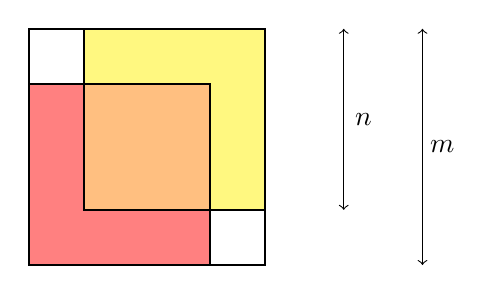
\begin{tikzpicture}
    \draw[thick] (0,0) rectangle (3,3);
    \draw[thick, fill=red!50] (0,0) rectangle (2.3,2.3);
    \draw[thick, fill=yellow!50] (0.7,0.7) rectangle (3, 3);
    \draw[thick, fill=orange!50] (0.7,0.7) rectangle (2.3, 2.3);
    \draw[<->] (4, 0.7)--(4, 3);
    \node at (4.25, 1.85) (n) {$n$};
    \draw[<->] (5, 0)--(5, 3);
    \node at (5.25, 1.5) (m) {$m$};
  \end{tikzpicture}
\end{center}
$m^2 = 2n^2$ હોવાથી $n$ બાજુવાળા બંને ચોરસો જ્યાં પરસ્પર આવરે છે
તે પ્રદેશનું ક્ષેત્રફળ બંને ચોરસોમાંથી કોઈ પણ ન આવરે એવા પ્રદેશના
ક્ષેત્રફળ જેટલું છે; એટલે કે નારંગી ચોરસનું ક્ષેત્રફળ છાયા વિનાના બે
ચોરસોનાં ક્ષેત્રફળોના સરવાળા જેટલું છે. તેથી નારંગી ચોરસની બાજુ $p$
અને છાયા વિનાના દરેક ચોરસની બાજુ $q$ હોય તો $p^2 = 2q^2$. પરંતુ હવે
$p < m$, $q < n$, $p, q \in \Nat$ સાથે
$\sqrt{2} = \nicefrac{p}{q}$. આ $m$ અને $n$ને શક્ય તેટલા નાના પસંદ
કર્યા હતા એ હકીકતનો વિરોધ કરે છે.

\emph{બીજી, ઔપચારિક રીતે.} $m^{2} = 2n^{2}$ હોવાથી $m$ યુગ્મ છે.
($x$ અયુગ્મ હોય તો $x^2$ અયુગ્મ છે તે બતાવવું સરળ છે.) તેથી કોઈ
$r \in \Nat$ માટે $m = 2r$. ફેરગોઠવણી કરતાં $2r^2 = n^2$,
    %                \begin{align*}
    %                  (2q)^{2} &= 2n^{2}\\
    %                  4q^{2} &= 2n^{2}\\
    %                  2q^{2} &= n^{2}
    %                \end{align*}
એટલે $n$ પણ યુગ્મ છે. આથી $m$ અને $n$ બંને યુગ્મ છે અને તેથી
$\nicefrac{m}{n}$ અપૂર્ણાંકને \emph{વધુ} સાદો કરી શકાય છે.
વિરોધાભાસ!
\end{proof}

પ્રસંગોપાત, આ આકૃતિમય સાબિતી આપણને \olref[his][set][mythology]{sec}ની
સામગ્રી ફરી વિચારવા દે છે. ટેનેનબાઉમ (1927--2006) પૂરેપૂરા આધુનિક
ગણિતજ્ઞ હતા; છતાં આ સાબિતી નિર્વિવાદપણે સુંદર, સંપૂર્ણ ચુસ્ત અને
ભૌમિતિક અંતઃપ્રજ્ઞા પર આધારિત છે!

કોઈ પણ રીતે જુઓ તો વાસ્તવિક સંખ્યાઓ સંમેય સંખ્યાઓ કરતાં ``વધુ
વિસ્તૃત'' છે. એક અર્થમાં સંમેય સંખ્યાઓમાં ``ખાલી જગ્યાઓ'' છે અને
વાસ્તવિક સંખ્યાઓ તે ભરે છે. વાયર્સ્ટ્રાસે સમજ્યું કે આ વાત વાસ્તવિક
સંખ્યાઓનો એક જ એવો ગુણધર્મ વર્ણવે છે જે તેમને સંમેય સંખ્યાઓથી જુદી
પાડે છે—એટલે પૂર્ણતા ગુણધર્મ: \emph{ઉચ્ચસીમા ધરાવતા વાસ્તવિક
સંખ્યાઓના દરેક અખાલી ગણને ન્યૂનતમ ઉચ્ચસીમા હોય છે.}

સંમેય સંખ્યાઓ પૂર્ણતા ગુણધર્મ ધરાવતી નથી તે સહેલાઈથી જોઈ શકાય છે.
દાખલા તરીકે $\sqrt{2}$ કરતાં નાની સંમેય સંખ્યાઓનો ગણ વિચારો, એટલે કે:
\[
  \Setabs{p \in \Rat}{p^2 < 2 \text{ અથવા }p < 0}
\]
આ ગણને સંમેય સંખ્યાઓમાં ઉચ્ચસીમા છે; દાખલા તરીકે તેના ઘટકો<
બધા $3$ કરતાં નાના છે. પરંતુ તેની ન્યૂનતમ ઉચ્ચસીમા શી છે? આપણે
`$\sqrt{2}$' કહેવા ઇચ્છીએ; પરંતુ હમણાં જ જોયું કે $\sqrt{2}$
\emph{સંમેય નથી}. અને $\sqrt{2}$ કરતાં મોટી કોઈ \emph{ન્યૂનતમ}
સંમેય સંખ્યા નથી. તેથી આ ગણને ઉચ્ચસીમા છે પરંતુ ન્યૂનતમ ઉચ્ચસીમા નથી.
પરિણામે સંમેય સંખ્યાઓ પૂર્ણતા ગુણધર્મ ધરાવતી નથી.

તેનાથી વિપરીત, સાતત્યક ``તાત્ત્વિક રીતે'' પૂર્ણતા ગુણધર્મ ધરાવવું
જોઈએ. આપણે માત્ર $\sqrt{2}$ને વાસ્તવિક સંખ્યા બનાવવા નથી ઇચ્છતા;
સંમેય રેખાની બધી ``ખાલી જગ્યાઓ'' ભરવા ઇચ્છીએ છીએ. ખરેખર, સાતત્યકમાં
પોતે કોઈ ``ખાલી જગ્યા'' ન રહે એવું ઇચ્છીએ છીએ. પૂર્ણતા વડે આપણને
બરાબર આ જ મળશે.




\olfileid{sfr}{arith}{cuts}
\olsection{$\Rat$થી $\Real$ સુધી}

મૂળ વાત એ છે કે પૂર્ણતા ગુણધર્મ બતાવે છે કે વાસ્તવિક રેખાનું કોઈ પણ
બિંદુ $\alpha$ એ રેખાને બે અર્ધભાગમાં બરાબર વહેંચે છે: એક ભાગ માટે
$\alpha$ ન્યૂનતમ ઉચ્ચસીમા છે અને બીજા માટે $\alpha$ મહત્તમ અધઃસીમા
છે. સંમેય સંખ્યાઓમાંથી વાસ્તવિક સંખ્યાઓની \emph{રચના} કરવા
ડેડેકિન્ડે સૂચવ્યું કે વાસ્તવિક સંખ્યાઓને સંમેય સંખ્યાઓનું વિભાજન કરતા
\emph{કાપ} તરીકે જ વિચારીએ. એટલે કે, $\sqrt{2}$ને એવા \emph{કાપ}
સાથે ઓળખીએ જે $< \sqrt{2}$ સંમેય સંખ્યાઓને $> \sqrt{2}$ સંમેય
સંખ્યાઓથી જુદી પાડે છે.

આ વિચારને સુઘડ બનાવીએ. સંમેય સંખ્યાઓને બે અર્ધભાગમાં કાપીએ તો કરેલા
વિભાજનને માત્ર તેના \emph{નીચલા} અર્ધભાગથી અનન્ય રીતે ઓળખી શકાય છે.
આથી ચોક્કસ વ્યાખ્યા નીચે મુજબ આપીએ છીએ:

\begin{defn}[કાપ]
\emph{કાપ} $\alpha$ એ સંમેય સંખ્યાઓનો એવો કોઈ પણ અખાલી ઉચિત
આરંભખંડ છે જેનો મહત્તમ ઘટક નથી. એટલે કે, $\alpha$ કાપ છે ત્યારે અને
માત્ર ત્યારે જ જ્યારે:
\begin{enumerate}
  \item \emph{અખાલી, ઉચિત}: $\emptyset \neq \alpha \subsetneq \Rat$
  \item \emph{આરંભિક}: બધા $p,q \in \Rat$ માટે, જો $p < q \in \alpha$ હોય તો $p \in \alpha$
  \item \emph{મહત્તમ ઘટક નહીં}: દરેક $p \in \alpha$ માટે કોઈ $q \in \alpha$ એવું છે કે $p < q$
\end{enumerate}
ત્યારે $\Real$ એ કાપોનો ગણ છે.
\end{defn}

હવે આપણે કહી શકીએ કે $\sqrt{2} = \Setabs{p \in \Rat}{p^2 < 2\text{
અથવા }p < 0}$. અલબત્ત, આ ખરેખર કાપ \emph{છે} તેની તપાસ કરવી પડે;
પરંતુ તે તપાસ \olref[check]{sec}માં રાખી છે.

પહેલાંની જેમ, કેટલીક વસ્તુઓની વ્યાખ્યા આપ્યા પછી હવે તેમના પરનાં
મૂળભૂત વિધેયો અને સંબંધોની વ્યાખ્યા કરવાની છે. એક સરળ વ્યાખ્યાથી શરૂ કરીએ:
\begin{align*}
  \alpha \leq \beta \text{ ત્યારે અને માત્ર ત્યારે જ જ્યારે }\alpha \subseteq \beta
\end{align*}
ક્રમની આ વ્યાખ્યા આપણને કેન્દ્રીય પરિણામ \emph{કહેવા} દે છે: કાપોનો
ગણ પૂર્ણતા ગુણધર્મ ધરાવે છે. પૂરેપૂરું લખીએ તો વિધાનનું સ્વરૂપ આવું છે.
$S$ એ ઉચ્ચસીમા ધરાવતો કાપોનો અખાલી ગણ હોય તો $S$ને ન્યૂનતમ ઉચ્ચસીમા
હોય છે. વધુ વિગતે: કોઈ કાપ $\lambda$ એ $S$ની ઉચ્ચસીમા છે, એટલે કે
$(\forall \alpha \in S)\alpha \subseteq \lambda$, અને $\lambda$ આવો
ન્યૂનતમ કાપ છે, એટલે કે
$(\forall \beta \in \Real)((\forall \alpha \in S)\alpha \subseteq \beta \lif \lambda \subseteq \beta)$.
હવે પરિણામની સાબિતી આ રહી:

\begin{thm}\ollabel{realcompleteness}
કાપોનો ગણ પૂર્ણતા ગુણધર્મ ધરાવે છે.
\end{thm}

\begin{proof}
$S$ એ ઉચ્ચસીમા ધરાવતો કાપોનો કોઈ અખાલી ગણ હોય. $\lambda = \bigcup S$ લો.
%\Setabs{p \in \Rat}{(\exists \alpha \in S)p \in \alpha}$$
પહેલાં આપણે દાવો કરીએ કે $\lambda$ કાપ છે:
\begin{enumerate}
\item $S$ અખાલી હોવાથી ઓછામાં ઓછો એક કાપ $S$માં છે, તેથી
$\emptyset \neq \lambda$. $S$ કાપોનો ગણ હોવાથી $\lambda
\subseteq \Rat$. $S$ને ઉચ્ચસીમા હોવાથી કોઈ $p \in \Rat$ દરેક કાપ
$\alpha \in S$માંથી ગેરહાજર છે. તેથી $p\notin \lambda$, અને પરિણામે
$\lambda \subsetneq \Rat$.
\item ધારો કે $p < q \in \lambda$. ત્યારે કોઈ $\alpha \in S$ એવું
છે કે $q \in \alpha$. $\alpha$ કાપ હોવાથી $p \in \alpha$. તેથી
$p \in \lambda$.
\item ધારો કે $p \in \lambda$. ત્યારે કોઈ $\alpha \in S$ એવું છે કે
$p \in \alpha$. $\alpha$ કાપ હોવાથી કોઈ $q \in \alpha$ એવું છે કે
$p < q$. તેથી $q \in \lambda$.
\end{enumerate}
આથી દાવો સાબિત થયો. વધુમાં, સ્પષ્ટપણે $(\forall \alpha \in S)\alpha
\subseteq \bigcup S = \lambda$, એટલે કે $\lambda$ એ $S$ની ઉચ્ચસીમા
છે. હવે ધારો કે $\beta \in \mathbb{R}$ પણ ઉચ્ચસીમા છે, એટલે કે
$(\forall \alpha \in S)\alpha \subseteq \beta$. કોઈ પણ $p \in \Rat$
માટે, જો $p \in \lambda$ હોય તો કોઈ $\alpha \in S$ માટે
$p \in \alpha$, તેથી $p \in \beta$. સામાન્યકરણ કરતાં
$\lambda \subseteq \beta$. આથી $\lambda$ એ $S$ની \emph{ન્યૂનતમ}
ઉચ્ચસીમા છે.
\sourcecorrection{OLARI-002}{મૂળની \texttt{cuts.tex}, પંક્તિઓ 61--65માં
\(S\)માં ઓછામાં ઓછો એક કાપ હોવાનો આધાર ભૂલથી “\(S\)ને ઉચ્ચસીમા છે”
એમ આપ્યો છે. આ તારણ \(S\) અખાલી છે એ ધારણાથી મળે છે; અહીં તે જ
યોગ્ય ધારણા લખી છે.}
\end{proof}

આ રીતે આપણને પૂર્ણતા ગુણધર્મ ધરાવતી ઘણી વસ્તુઓ મળી છે. આને કહેવાની
એક રીત એ છે કે આપણા કાપોમાં કોઈ ``ખાલી જગ્યા'' નથી. (આથી સંમેય
સંખ્યાઓને બદલે વાસ્તવિક સંખ્યાઓના વધુ ``કાપ'' લેવાથી કોઈ રસપ્રદ નવી
વસ્તુઓ નહીં મળે.)

હવે વાસ્તવિક સંખ્યાઓ પર કેટલીક ક્રિયાઓ વ્યાખ્યાયિત કરવી પડશે.
દરેક $p \in \Rat$ માટે $p_\Real = \Setabs{q \in \Rat}{q < p}$ એમ
ઠરાવીને આપણે પહેલાં સંમેય સંખ્યાઓને વાસ્તવિક સંખ્યાઓમાં સ્થાપિત કરીએ છીએ.
પછી વ્યાખ્યા કરીએ છીએ:
\begin{align*}
  \alpha + \beta &= \Setabs{p + q}{p \in \alpha \land q \in \beta}\\
%  \alpha - \beta &\defis \Setabs{p - q}{p \in \alpha \land q \in \Rat \setminus \beta}\\
  \alpha \times \beta &=
  \Setabs{p \times q}{0 \leq p \in \alpha \land 0 \leq q \in \beta} \cup 0^\mathbb{R} & \text{ જો }\alpha, \beta \geq 0_\Real
%  \alpha \div \beta &\defis
%  \Setabs{\nicefrac{p}{q}}{p \in \alpha \land q \in \Rat \setminus \beta}  & \text{ જો }\alpha \geq 0_\Real, \beta > 0_\Real
\end{align*}
ગુણાકારના બીજા કિસ્સા સંભાળવા પહેલાં નીચે મુજબ લો: %કે $0_\Real \times \alpha = 0_\Real = \alpha \times 0_\Real$, અને ઉમેરો:
\begin{align*}
  -\alpha &= \Setabs{p - q}{p < 0 \land q \notin \alpha}
\end{align*}
અને પછી એમ ઠરાવો કે:
\begin{align*}
  \alpha \times \beta &\defis
  \begin{cases}
    \mathord{-}\alpha \times \mathord{-}\beta &\text{ જો }\alpha < 0_\Real\text{ અને }\beta < 0_\Real\\
    \mathord{-}(\mathord{-}\alpha \times \beta) &\text{ જો }\alpha < 0_\Real \text{ અને }\beta > 0_\Real\\
    \mathord{-}(\alpha \times \mathord{-}\beta) &\text{ જો }\alpha > 0_\Real \text{ અને }\beta < 0_\Real
  \end{cases}
\end{align*}
આમાંની દરેક વ્યાખ્યા હંમેશાં કાપ જ આપે છે તેની તપાસ કરવી પડશે.
છેલ્લે, આ રીતે વ્યાખ્યાયિત કાપોનો વ્યવહાર બરાબર જેવો હોવો જોઈએ
તેવો જ છે તેનું સરળ પરંતુ લાંબું નિદર્શન કરવું પડશે. આ બધું
\olref[check]{sec}માં રાખીએ છીએ.



\olfileid{sfr}{arith}{ref}
\olsection{કેટલાક તાત્ત્વિક પ્રતિચિંતનો}

પ્રાવિધિક વિગતો આટલી થઈ. પરંતુ તેનાથી સિદ્ધ શું થયું?

એવું લગભગ નિર્વિવાદ છે કે તેનાથી આપણને થોડું {સુંદર} શુદ્ધ ગણિત
મળ્યું. ઉપરાંત કેટલીક ગહન વૈચારિક સિદ્ધિઓ મળી. પૂર્ણતા ગુણધર્મ
વાસ્તવિક અને સંમેય સંખ્યાઓ વચ્ચેનો નિર્ણાયક તફાવત વ્યક્ત કરે છે એવું
જોવું એક ગહન અંતર્દૃષ્ટિ હતું. વધુમાં, ડેડેકિન્ડ કાપ તરીકે વાસ્તવિક
સંખ્યાઓની સ્પષ્ટ રચના વિશ્લેષણના વિષયને મજબૂત પાયો આપે છે. કાપો
\emph{પૂર્ણ ક્રમિત ક્ષેત્ર} બનાવે છે, તેથી આ ખ્યાલ સુસંગત છે તે આપણે જાણીએ છીએ.

આ બધું સ્વીકાર્યા પછી પણ આ સિદ્ધિઓ વિશે કેટલીક શંકાઓ જણાવવી જોઈએ.

પહેલી વાત, વાસ્તવિક સંખ્યાઓને કાપો તરીકે વિચારવી એ તેમના પરિચિત
(કદાચ અનંત) દશાંશ વિસ્તરણોના રૂપમાં વિચારવા કરતાં \emph{વધુ} ચુસ્ત
છે કે નહીં તે સ્પષ્ટ નથી. વાસ્તવિક સંખ્યાઓની આ બીજી ``રચના'' કોશી
શ્રેણી વડે થતી રચના સાથે થોડું સામ્ય ધરાવે છે; પરંતુ હકીકતમાં
સત્તરમી સદીના આરંભથી ગણિતજ્ઞો તેને મૂળભૂત રીતે જાણતા હતા
(\olref[cauchy]{sec} જુઓ). ચુસ્તતામાં ખરેખરનો વધારો વાસ્તવિક સંખ્યાઓ
પૂર્ણતા ગુણધર્મ ધરાવે છે એ સમજવાથી થયો. ચોક્કસ ગણો તરીકે વાસ્તવિક
સંખ્યાઓ રચવાની ક્ષમતા કદાચ પોતાની રીતે એટલી રસપ્રદ નથી.

પૂર્ણાંકોનું કે સંમેય સંખ્યાઓનું (ઘણું સરળ) અંકગણિતીકરણ તે ક્ષેત્રોમાં
ચુસ્તતા વધારે છે કે નહીં તે તો હજી ઓછું સ્પષ્ટ છે. અહીં એક સરળ અવલોકન
ઉપયોગી છે. પ્રાકૃતિક સંખ્યાઓની ક્રમયુક્ત જોડોના સામ્ય વર્ગો તરીકે
પૂર્ણાંકોની \emph{રચના} કર્યા પછી, પૂર્ણાંકોની ક્રમયુક્ત જોડોના સામ્ય
વર્ગો તરીકે સંમેય સંખ્યાઓની રચના કર્યા પછી અને સંમેય સંખ્યાઓના ગણો
તરીકે વાસ્તવિક સંખ્યાઓ રચ્યા પછી આપણે તરત જ એ રચનાઓને \emph{ભૂલી
જઈએ છીએ}. ખાસ કરીને, ગણિતીય સાબિતીમાં કોઈ આ રચનાઓને ક્યારેય
\emph{ઉપયોગમાં લેવા} ઇચ્છશે નહીં (અલબત્ત, રચનાઓનો વ્યવહાર ધાર્યા મુજબ
છે એવી સાબિતી સિવાય). પ્રાકૃતિક સંખ્યાઓના ગણોના ગણોના ગણોના ગણોના
ગણોના ગણોના કોઈ ગણ વિશે બોલવા કરતાં સીધું કોઈ વાસ્તવિક સંખ્યા વિશે
બોલવું ઘણું સરળ છે.
%(કારણ કે વાસ્તવિક સંખ્યાઓ સંમેય સંખ્યાઓના ગણો તરીકે રચાઈ; અને સંમેય સંખ્યાઓ પૂર્ણાંકોની ક્રમયુક્ત જોડોના સામ્ય વર્ગો, એટલે કે પૂર્ણાંકોના ગણોના ગણોના ગણો તરીકે રચાઈ; વગેરે.)
%2/3 = [2,3]
%  એટલે કે {<2,3>, ... }
%  { {{2},{2,3}}, ... }
%
%વાસ્તવિક સંખ્યાઓ છે
%  સંમેય સંખ્યાઓના ગણો
%
%સંમેય સંખ્યાઓ છે
%  પૂર્ણાંકોના ગણોના ગણોના ગણો
%
%પૂર્ણાંકો છે
%  પ્રાકૃતિક સંખ્યાઓના ગણોના ગણોના ગણો

આ વ્યાખ્યાઓ આપણને પૂર્ણાંકો, સંમેય સંખ્યાઓ કે વાસ્તવિક સંખ્યાઓ
\emph{અધિભૌતિક અર્થમાં શું છે} તે કહે છે એવો દાવો સૌથી વધુ
શંકાસ્પદ છે. એટલે કે, વાસ્તવિક સંખ્યાઓ (ધારો કે) ચોક્કસ ગણો
(ગણોના ગણોના ગણો\ldots) જ \emph{છે} એ શંકાસ્પદ છે. આવા મતનો મુખ્ય
અવરોધ એ છે કે રચના ઘણી જુદી રીતે થઈ શકી હોત. વાસ્તવિક સંખ્યાઓના
કિસ્સામાં ખરેખર રસપ્રદ રીતે જુદી રચનાઓ છે (\olref[cauchy]{sec} જુઓ).
પરંતુ તદ્દન જુદી રચનાઓ મેળવવાની આ એક નજીવી રીત છે: જેમ
\olref[sfr][rel][ref]{sec}માં જોયું, ક્રમયુક્ત જોડની વ્યાખ્યા સહેજ જુદી
રીતે કરી શકાઈ હોત; આ વૈકલ્પિક ખ્યાલ વાપર્યો હોત તો આપણી રચનાઓ એટલી
જ સારી રીતે કામ કરત, પરંતુ અંતે મળતી વસ્તુઓ જુદી હોત. આમ પૂર્ણાંકો,
સંમેય સંખ્યાઓ અને વાસ્તવિક સંખ્યાઓની ઘણી હરીફ ગણસૈદ્ધાંતિક રચનાઓ છે.
હવે પૂર્ણાંકો (ધારો કે) \emph{આ} ગણો છે, \emph{તે} નહીં, એવો દાવો
મનસ્વી (અને મૂંઝવણજનક) થશે. (\olref[sfr][rel][ref]{sec}ની જેમ આ પણ
\citealt{Benacerraf1965}એ પ્રસિદ્ધ કરેલી દલીલનું એક દૃષ્ટાંત છે.)

બીજો મુદ્દો પણ ઉઠાવવો જોઈએ: આપણી રચનાઓમાં કશુંક બહુ \emph{વિચિત્ર}
છે. આપણે પ્રાકૃતિક સંખ્યાઓથી શરૂ કર્યું. પછી પૂર્ણાંકો રચ્યા અને
``પૂર્ણાંકોનું $0$'', એટલે કે $\equivrep{0,0}{\Intequiv}$ રચ્યું.
પરંતુ $0 \neq \equivrep{0,0}{\Intequiv}$. ખરેખર, આપણી રચનાઓ મુજબ
\emph{કોઈ પણ} પ્રાકૃતિક સંખ્યા પૂર્ણાંક નથી. આ ખૂબ જ પ્રતિઅંતઃપ્રજ્ઞ
લાગે છે. વળી \olref[sfr][set][imp]{sec}માં આપણે બહુ દલીલ કર્યા વિના
$\Nat \subseteq \Rat$ એવો દાવો કર્યો હતો. જો આ રચનાઓ સંખ્યાઓ
\emph{બરાબર શું છે} તે કહેતી હોય, તો એ દાવો સહેજે ખોટો હતો.

હવે થોડું દૂરથી જોઈએ તો આપણે ક્યાં પહોંચ્યા? સહજ ગણસિદ્ધાંતમાં કામ
કરીને અને પ્રાકૃતિક સંખ્યાઓને આપેલી માનીને, પૂર્ણાંકો, સંમેય સંખ્યાઓ
અને વાસ્તવિક સંખ્યાઓને ચોક્કસ ગણો \emph{તરીકે} ગણી શકીએ છીએ. આ અર્થમાં
આ વસ્તુઓના સિદ્ધાંતોને ગણસિદ્ધાંતમાં \emph{સ્થાપિત} કરી શકીએ છીએ.
પરંતુ આ સ્થાપનનું તાત્ત્વિક મહત્ત્વ એટલું સીધું નથી.

અલબત્ત, આમાંથી કંઈ અંતિમ શબ્દ નથી!{} મુદ્દો માત્ર આ છે: વાસ્તવિક
સંખ્યાઓનું અંકગણિતીકરણ ગહન તાત્ત્વિક મહત્ત્વ \emph{ધરાવે છે} એવું
બતાવવા માટે કેટલીક વધારાની \emph{તાત્ત્વિક} દલીલ જરૂરી થશે.

%વધુમાં: આ આખા પ્રકરણ દરમિયાન આપણે પ્રાકૃતિક સંખ્યાઓને સીધી
%\emph{આપેલી} માની છે. પરંતુ તેમના વિશે આપણે શું કરી શકીએ?
%આગળનું પ્રકરણ એ જ વિષય લે છે.




\olfileid{sfr}{arith}{check}
\olsection{ક્રમિત મંડળો અને ક્ષેત્રો}

આ આખા પ્રકરણમાં આપણે દાવો કર્યો કે અમુક વ્યાખ્યાઓનો વ્યવહાર
``જેવો હોવો જોઈએ તેવો'' છે. આ પ્રાવિધિક પરિશિષ્ટમાં તેનો અર્થ
સ્પષ્ટ કરીશું અને વ્યાખ્યાઓનો વ્યવહાર ``યોગ્ય રીતે'' થાય છે તે
(કેવી રીતે બતાવવું તેની રૂપરેખા) આપીશું.

\olref[int]{sec}માં આપણે $\Int$ પર સરવાળો અને ગુણાકાર વ્યાખ્યાયિત
કર્યા. વ્યાખ્યા મુજબ આ ક્રિયાઓ $\Int$ને આપણે ``ઇચ્છીએ તેવું''
સંરચના આપે છે એવું બતાવવું છે. ખાસ કરીને, અહીંની સંરચના સમક્રમી
મંડળની છે.

\begin{defn}
	\emph{સમક્રમી મંડળ} એવો ગણ $S$ છે જેમાં નિશ્ચિત ઘટકો $0$ અને $1$
	તથા ક્રિયાઓ $+$ અને $\times$ હોય અને જે નીચેના આઠ સૂત્રો સંતોષે:
	\begin{align*}
		\emph{સંગઠિતતા}&&a + (b+ c) & = (a + b) + c \\
		&& (a \times b) \times c & = a \times (b\times c)\\
		\emph{સમક્રમિતા}&&a + b &= b+ a  \\
		&&  a \times b&= b\times a\\
		\emph{એકમો}&&a + 0 &= a \\
		&& a \times 1 &= a\\
		\emph{યોજક વ્યસ્ત}&&(\exists b\in S)0&=a + b\\
		\emph{વિતરણાત્મકતા}&&a \times (b+ c ) &= (a \times b) + (a \times c)
	\end{align*}
	અહીં ગર્ભિત રીતે આ બધાં સૂત્રોના સર્વપરિમાણકો $S$ પૂરતા
	મર્યાદિત છે. એ પણ નોંધો કે અહીંના $0$ અને~$1$ નામના ઘટકો એ જ
	નામ ધરાવતી પ્રાકૃતિક સંખ્યાઓ હોવા જરૂરી નથી.
\end{defn}

તેથી પૂર્ણાંકો સમક્રમી મંડળ બનાવે છે કે નહીં તે ચકાસવા માટે આ આઠે
શરતો સંતોષાય છે એટલું જ ચકાસવાનું રહે છે. કોઈ શરત સ્થાપવી {મુશ્કેલ}
નથી, પણ એ કામ થોડું શ્રમસાધ્ય છે. દાખલા તરીકે, સરવાળાના કિસ્સામાં
\emph{સંગઠિતતા} આ રીતે સાબિત કરી શકાય:

\begin{proof}
$i, j, k \in \Int$ નિશ્ચિત કરો. ત્યારે એવા $a_1, b_1, a_2, b_2, a_3, b_3 \in
\Nat$ છે કે $i = \equivrep{a_1, b_1}{}$, $j =
\equivrep{a_2,b_2}{}$ અને $k = \equivrep{a_3, b_3}{}$. (વાંચવામાં
સરળતા રહે તે માટે આપણે ``$\equivrep{x, y}{\Intequiv}$''ને બદલે
``$\equivrep{x, y}{}$'' લખીએ છીએ; આ આખા વિભાગમાં એમ જ કરીશું.) હવે:
\begin{align*}
	i + (j + k) &= \equivrep{a_1, b_1}{}+(\equivrep{a_2, b_2}{} + \equivrep{a_3, b_3}{}) \\
	&= \equivrep{a_1,  b_1}{} + \equivrep{a_2+a_3, b_2+b_3}{}\\
	&= \equivrep{a_1 + (a_2 + a_3), b_1 + (b_2 + b_3)}{}\\
	&= \equivrep{(a_1 + a_2) + a_3, (b_1 + b_2) + b_3}{}\\
	&= \equivrep{a_1 + a_2, b_1 + b_2}{} + \equivrep{a_3, b_3}{}\\
	&= (\equivrep{a_1, b_1}{} + \equivrep{a_2, b_2}{}) + \equivrep{a_3, b_3}{}\\
	&= (i+j) + k
\end{align*}
અહીં $\Nat$ પરના સરવાળાના વ્યવહારનો આપણે નિઃસંકોચ ઉપયોગ કર્યો છે.
\end{proof}

એ જ રીતે \emph{યોજક વ્યસ્ત} આ રીતે સાબિત કરી શકાય:

\begin{proof}
$i \in \Int$ નિશ્ચિત કરો; ત્યારે કોઈ $a,b \in \Nat$ માટે $i =
\equivrep{a,b}{}$. $j = \equivrep{b,a}{} \in \Int$ લો. પ્રાકૃતિક
સંખ્યાઓના વ્યવહારનો ઉપયોગ કરતાં $(a+b) + 0 = 0 + (a+b)$, તેથી
વ્યાખ્યા મુજબ $\tuple{a+b, b+a} \sim_\Int \tuple{0,0}$, અને તેથી
$\equivrep{a+b, b+a}{} = \equivrep{0, 0}{} = 0_\Int$. હવે $i + j =
\equivrep{a,b}{}+\equivrep{b,a}{}=\equivrep{a+b, b+a}{}= \equivrep{0,
0}{} = 0_\Int$.
\end{proof}

અને \emph{વિતરણાત્મકતા}ની સાબિતી આ રહી:

\begin{proof}
ઉપરની જેમ $i = \equivrep{a_1, b_1}{}$, $j =
\equivrep{a_2,b_2}{}$ અને $k = \equivrep{a_3, b_3}{}$ નિશ્ચિત કરો. હવે:
\begin{align*}
	i \times (j + k)
	&= \equivrep{a_1, b_1}{} \times (\equivrep{a_2,b_2}{} + \equivrep{a_3, b_3}{})\\
	&= \equivrep{a_1, b_1}{} \times \equivrep{a_2 + a_3,b_2+b_3}{}\\
	&= \equivrep{a_1  (a_2 + a_3) + b_1  (b_2+b_3), a_1  (b_2 + b_3) + b_1 (a_2 + a_3)}{}\\
	&= \equivrep{a_1 a_2 + a_1a_3 + b_1 b_2+b_1b_3, a_1 b_2 + a_1b_3 + a_2b_1 + a_3b_1}{}\\
%		&= \equivrep{a_1 a_2 + b_1b_2 + a_1a_3 + b_1 b_2+b_1b_3, a_1 b_2 + a_1b_3 + a_2b_1 + a_3b_1}{}\\
	&= \equivrep{a_1a_2 + b_1b_2, a_1b_2 + a_2b_1}{} + \equivrep{a_1a_3 + b_1b_3, a_1b_3 + a_3b_1}{}\\
	&= (\equivrep{a_1, b_1}{} \times \equivrep{a_2,b_2}{}) + (\equivrep{a_1, b_1}{} \times  \equivrep{a_3, b_3}{})\\
	&= (i \times j) + (i \times k)
\end{align*}
\end{proof}

બાકીની પાંચ શરતોની સાબિતી કસરત તરીકે છોડી દઈએ છીએ. એ કરી લઈએ
પછી આપણે બતાવ્યું હશે કે $\Int$ સમક્રમી મંડળ બનાવે છે, એટલે કે સરવાળો
અને ગુણાકારનો (વ્યાખ્યાયિત કરેલો) વ્યવહાર જેવો હોવો જોઈએ તેવો છે.

\begin{prob}
$\Int$ સમક્રમી મંડળ છે તે સાબિત કરો.
\end{prob}

પરંતુ આપણું કામ પૂરું થયું નથી. $\Int$ પર સરવાળો અને ગુણાકાર
વ્યાખ્યાયિત કરવા ઉપરાંત આપણે ક્રમસંબંધ $\leq$ પણ વ્યાખ્યાયિત કર્યો
હતો અને તેનો વ્યવહાર પણ જેવો હોવો જોઈએ તેવો છે એ ચકાસવું પડે. વધુ
ચોક્કસ રીતે, $\Int$ \emph{ક્રમિત} મંડળ બનાવે છે એવું બતાવવું પડશે.\footnote{
	\olref[sfr][rel][ord]{def:linearorder}માંથી યાદ કરો કે સંપૂર્ણ ક્રમ
	સ્વવાચક, પરંપરિત, વિસંમિત અને તુલનાયુક્ત સંબંધ છે. ક્રમસંબંધોના
	સંદર્ભમાં તુલનાયુક્તતાને ક્યારેક \emph{ત્રિવિકલ્પતા} કહે છે, કારણ કે
	કોઈ પણ $a$ અને $b$ માટે $a \leq b \lor a = b \lor a \geq b$.}

\begin{defn}
\emph{ક્રમિત મંડળ} એવું સમક્રમી મંડળ છે જેમાં સંપૂર્ણ ક્રમસંબંધ
$\leq$ પણ હોય અને નીચેની શરતો સંતોષાય:
\begin{align*}
	a \leq b &\lif a + c \leq b + c\\
	(a \leq b \land 0 \leq c) &\lif a \times c \leq b \times c
\end{align*}
\end{defn}

\begin{prob}
$\Int$ ક્રમિત મંડળ છે તે સાબિત કરો.
\end{prob}

અગાઉની જેમ રચાયેલું~$\Int$ ક્રમિત મંડળ છે એવું બતાવવું શ્રમસાધ્ય
પણ નિયમિત કામ છે. તે તમારા માટે છોડી દઈએ છીએ.

આમ પૂર્ણાંકોનું કામ પૂરું થયું. હવે સંમેય સંખ્યાઓ માટે આવી જ બાબતો
બતાવવી છે. ખાસ કરીને $+$, $\times$ અને $\leq$ની આપેલી વ્યાખ્યાઓ તળે
સંમેય સંખ્યાઓ ક્રમિત \emph{ક્ષેત્ર} બનાવે છે એવું બતાવવું છે:
\begin{defn}\ollabel{orderedfield}
\emph{ક્રમિત ક્ષેત્ર} એવું ક્રમિત મંડળ છે જે આ વધારાની શરત પણ સંતોષે:
\begin{align*}
	\emph{ગુણાકારી વ્યસ્ત}& & (\forall a \in S \setminus \{0\})(\exists b \in S) a\times b& = 1
\end{align*}
\end{defn}

$\Int$ ક્રમિત મંડળ બનાવે છે એવું બતાવી લીધા પછી $\Rat$ ક્રમિત ક્ષેત્ર
બનાવે છે એવું બતાવવું સરળ, પણ શ્રમસાધ્ય છે.

\begin{prob}
$\Rat$ ક્રમિત ક્ષેત્ર છે તે સાબિત કરો.
\end{prob}

પૂર્ણાંકો અને સંમેય સંખ્યાઓનું કામ પૂરું કર્યા પછી માત્ર વાસ્તવિક
સંખ્યાઓ બાકી રહે છે. ખાસ કરીને, $\Real$ \emph{પૂર્ણ} ક્રમિત ક્ષેત્ર,
એટલે કે પૂર્ણતા ગુણધર્મ ધરાવતું ક્રમિત ક્ષેત્ર, બનાવે છે એવું બતાવવું
પડે. \olref[cuts]{realcompleteness}માં $\Real$ પૂર્ણતા ગુણધર્મ ધરાવે
છે એવું સ્થાપ્યું હતું. પરંતુ $\Real$ ક્રમિત ક્ષેત્ર છે તેની
(કંટાળાજનક) ચકાસણીની વિગતો હજી બાકી છે.

આ શ્રમસાધ્ય કસરત તરફ વળતાં પહેલાં થોડી વધુ ``તાત્કાલિક'' બાબતો
ચકાસવી પડશે. દાખલા તરીકે, કોઈ પણ કાપો $\alpha$ અને $\beta$ માટે
વ્યાખ્યાયિત કરેલો $\alpha + \beta$ ખરેખર \emph{કાપ} જ છે તેની ખાતરી
કરવી પડશે. તેની સાબિતી આ રહી:

\begin{proof}
$\alpha$ અને $\beta$ બંને કાપ હોવાથી $\alpha + \beta = \Setabs{p
+ q}{p \in \alpha \land q \in \beta}$ એ $\Rat$નો અરિક્ત ઉચિત ઉપગણ
છે. હવે કોઈ $p \in \alpha$ અને $q \in \beta$ માટે $x < p + q$ ધારો.
ત્યારે $x - p < q$, તેથી $x - p \in \beta$, અને $x = p + (x - p) \in
\alpha + \beta$. તેથી $\alpha + \beta$ એ $\Rat$નો આરંભિક ખંડ છે.
અંતે, કોઈ પણ $p + q \in \alpha + \beta$ માટે, $\alpha$ અને $\beta$
બંને કાપ હોવાથી એવા $p_1 \in \alpha$ અને $q_1 \in \beta$ છે કે
$p < p_1$ અને $q < q_1$; તેથી $p + q < p_1 + q_1 \in \alpha +
\beta$; આમ $\alpha + \beta$ને કોઈ મહત્તમ ઘટક નથી.
\end{proof}

આવી જ મહેનતથી તમે ચકાસી શકશો કે $\alpha - \beta$, $\alpha \times
\beta$ અને $\alpha \div \beta$ પણ કાપ છે (છેલ્લા કિસ્સામાં $\beta$
શૂન્ય-કાપ હોય તે કિસ્સો અવગણવો). એ પણ આપણે તમારા માટે જ છોડી દઈએ છીએ.

\begin{prob}
$\Real$ ક્રમિત ક્ષેત્ર છે તે સાબિત કરો.
\end{prob}

હવે એક નાની અધૂરી વિગત પૂરી કરીએ. \olref[cuts]{sec}માં આપણે સૂચવ્યું
હતું કે $\sqrt{2} = \Setabs{p \in \Rat}{p < 0 \text{ અથવા }p^2 < 2}$
લઈ શકાય. પરંતુ આ ગણ \emph{કાપ} છે એવું બતાવવું પડે. તેની સાબિતી આ રહી:

\begin{proof}
સ્પષ્ટપણે આ સંમેય સંખ્યાઓનો અરિક્ત ઉચિત આરંભિક ખંડ છે; તેથી તેને
મહત્તમ ઘટક નથી એટલું બતાવવું પૂરતું છે. ખાસ કરીને, $p^2 < 2$ ધરાવતી
ધન સંમેય સંખ્યા $p$ અને $q = \frac{2p+2}{p+2}$ હોય ત્યારે $p < q$ અને
$q^2 < 2$ બંને બતાવવાં પૂરતાં છે. $p < q$ જોવા માટે માત્ર નોંધો:
\begin{align*}
	p^2 &< 2\\
	p^2 + 2p &< 2 + 2p\\
	p(p + 2) &< 2 + 2p\\
	p &< \tfrac{2+2p}{p+2} = q
\end{align*}
$q^2 < 2$ જોવા માટે માત્ર નોંધો:
\begin{align*}
	p^2 &< 2\\
	2p^2 + 4p + 2 &< p^2 + 4p+ 4\\
	4p^2 + 8p + 4 &< 2(p^2 + 4p + 4)\\
	(2p+2)^2 & <2(p+2)^2\\
	\tfrac{(2p+2)^2}{(p+2)^2} &< 2\\
	q^2 &< 2
\end{align*}
\end{proof}



\olfileid{sfr}{arith}{cauchy}

\olsection{પરિશિષ્ટ: કોશી શ્રેણીઓ તરીકે વાસ્તવિક સંખ્યાઓ}

\olref[cuts]{sec}માં આપણે વાસ્તવિક સંખ્યાઓની રચના ડેડેકિન્ડ કાપો
તરીકે કરી. આ વિભાગમાં એક વૈકલ્પિક રચના સમજાવીશું. તે કોશીએ
(જેને હવે આપણે કોશી શ્રેણી કહીએ છીએ તેની) આપેલી વ્યાખ્યા પર આધારિત
છે; પરંતુ આ વ્યાખ્યાનો ઉપયોગ કરીને વાસ્તવિક સંખ્યાઓની \emph{રચના}
કરવાનું શ્રેય ઓગણીસમી સદીના બીજા લેખકોને, ખાસ કરીને વાયરસ્ટ્રાસ,
હાઇને, મેરે અને કૅન્ટૉરને જાય છે. (સરસ ઇતિહાસ માટે
\citeauthor{OConnorRobertson:RN} \citeyear{OConnorRobertson:RN} જુઓ.)

ઓગણીસમી સદી સુધી પહોંચતાં પહેલાં સિમોન સ્ટેવિન (1548--1620)નો વિચાર
કરવો યોગ્ય છે. ટૂંકમાં, સ્ટેવિને સમજ્યું કે દરેક વાસ્તવિક સંખ્યાને
તેના દશાંશ વિસ્તરણ દ્વારા વિચારી શકાય. તેથી $\sqrt{2}$ જેવી અસંમેય
સંખ્યાનું પણ સરસ દશાંશ વિસ્તરણ છે, જે આ રીતે શરૂ થાય છે:
\[
	1.41421356237\ldots
\]
ગણસિદ્ધાંતમાં દશાંશ વિસ્તરણોના પ્રતિરૂપ બનાવવા બહુ સરળ છે: તેમને
$d \colon \Nat \to \Nat$ વિધેયો તરીકે વિચારો, જ્યાં $d(n)$ આપણને
રસ હોય તે $n$મું દશાંશ સ્થાન છે. પછી દશાંશ ચિહ્નની પહેલાં આવતા
વાસ્તવિક સંખ્યાના ભાગને (અહીં માત્ર $1$ને) સંભાળવા વ્યાખ્યામાં થોડો
ફેરફાર કરવો પડશે. દાખલા તરીકે $0.999\ldots = 1$ની ખાતરી કરવા માટે
બીજો ફેરફાર (એક સામ્ય સંબંધ) પણ કરવો પડશે. પરંતુ સ્ટેવિનની રીત મુજબ
ગણસિદ્ધાંતમાં વાસ્તવિક સંખ્યાઓની પૂરેપૂરી ચુસ્ત રચના આપવી મુશ્કેલ નથી.

અહીં સ્ટેવિન આપણો મુખ્ય વિષય નથી. (સ્ટેવિન વિશે વધુ માટે
\citealt{KatzKatz2012} જુઓ.) પરંતુ આ રહ્યો તેની નજીકનો એક વિચાર.
$\sqrt{2}$ના દશાંશ વિસ્તરણને સીધું લેવાને બદલે વધુ ને વધુ ચોક્કસ
વિસ્તરણો લઈને $\sqrt{2}$નાં વધુ ને વધુ ચોક્કસ સંમેય આસન્ન મૂલ્યોની
એક \emph{શ્રેણી} વિચારી શકાય:
\[
1, 1.4, 1.414, 1.4142, 1.41421,\ldots
\]
વાસ્તવિક સંખ્યાઓને ``વધુ ને વધુ સારા આસન્ન મૂલ્યો'' દ્વારા વિચારી
શકાય એ વિચાર આપણને અંતર્દૃષ્ટિઓના બીજા ક્રમનો આધાર આપે છે (જેમ
$\Int$માંથી $\Rat$ અથવા $\Nat$માંથી $\Int$ રચતી વખતે મળેલી
અંતર્દૃષ્ટિઓ). મૂળભૂત અંતર્દૃષ્ટિઓ આ છે:
\begin{enumerate}
	\item દરેક વાસ્તવિક સંખ્યાને (કદાચ અનંત) દશાંશ વિસ્તરણ તરીકે લખી
	શકાય છે.
	\item (કદાચ અનંત) દશાંશ વિસ્તરણમાં સમાયેલી માહિતીને સંમેય સંખ્યાઓની
	શ્રેણીથી પણ એટલી જ રીતે રજૂ કરી શકાય છે.
	\item સંમેય સંખ્યાઓની શ્રેણીને $\Nat$માંથી $\Rat$માં જતા વિધેય
	તરીકે વિચારી શકાય; શ્રેણીની $n$મી સંમેય સંખ્યાને $f(n)$ લો.
\end{enumerate}
અલબત્ત, $\Nat$માંથી $\Rat$માં જતું \emph{કોઈ પણ} વિધેય આપણને વાસ્તવિક
સંખ્યા આપશે એવું નથી. દાખલા તરીકે, આ વિધેય વિચારો:
\[
	f(n) =\begin{cases}
			1 & \text{જો }n\text{ અયુગ્મ હોય}\\
			0 &\text{જો }n\text{ યુગ્મ હોય}
		\end{cases}
\]
અહીં મૂળ ચિંતા એ છે કે $0,1,0,1,0,1,0,\ldots$ શ્રેણી કોઈ વાસ્તવિક
સંખ્યા તરફ ``નજીક જતી'' જણાતી નથી. તેથી કોઈ વાસ્તવિક સંખ્યા તરફ
નજીક જતી શ્રેણીઓ જ વિચારવામાં આવે એની ખાતરી કરવા માટે આપણે કોઈ
\emph{લક્ષ} ધરાવતી શ્રેણીઓ પૂરતું ધ્યાન મર્યાદિત કરવું પડશે.

લક્ષનો વિચાર આપણે \olref[his][set][limits]{sec}માં જોઈ ચૂક્યા છીએ.
પરંતુ ત્યાં લીધેલી વ્યાખ્યા \emph{બરાબર} એ જ રીતે અહીં લઈ શકીએ નહીં.
ત્યાં ``$(\forall \epsilon>0)$'' અભિવ્યક્તિમાં વાસ્તવિક સંખ્યાઓ પરનું
પરિમાણીકરણ ગર્ભિત હતું; અને આપણે વાસ્તવિક સંખ્યાઓ પરનાં વિધેયોના
લક્ષ વિચારતા હતા. એટલે એ વ્યાખ્યાનો ઉપયોગ કરીએ તો જે વાસ્તવિક સંખ્યાઓની
\emph{રચના} કરવાનું આપણું લક્ષ છે તેને પહેલાંથી જ માની લઈએ. સદભાગ્યે,
લક્ષના અત્યંત નજીકના એક વિચારથી કામ ચાલી શકે છે.
\begin{defn}\ollabel{def:CauchySequence}
  વિધેય $f: \Nat \to \Rat$ \emph{કોશી શ્રેણી} હોય ત્યારે અને માત્ર
  ત્યારે જ જ્યારે દરેક ધન $\epsilon \in \Rat$ માટે $(\exists \ell \in
  \Nat)(\forall m, n > \ell)|f(m) - f(n)| < \epsilon$.
\end{defn}

લક્ષનો સામાન્ય વિચાર પહેલાં જેવો જ છે: તમને ($\epsilon$થી મપાતું)
અમુક ચોકસાઈનું સ્તર જોઈતું હોય તો જોવા માટે એક ``વિસ્તાર'' (એટલે કે
$\ell$ કરતાં મોટું કોઈ પણ આગત) મળે છે. આપણી શ્રેણી $1$, $1.4$,
$1.414$, $1.4142$, $1.41421$\ldots{}ને લક્ષ છે એવું જોવું પણ સરળ છે:
$\sqrt{2}$નું $\nicefrac{1}{10^{n}}$ જેટલી ત્રુટિની અંદર આસન્ન મૂલ્ય
જોઈતું હોય તો $n$મા ઘટક પછીના કોઈ પણ ઘટકને જુઓ.

ત્યારે પહેલો સ્વાભાવિક વિચાર એવો આવે કે કોઈ પણ કોશી શ્રેણી બસ એક
વાસ્તવિક સંખ્યા \emph{છે}. પરંતુ $\Int$ અને $\Rat$ની રચનાઓની જેમ આ
વિચાર બહુ ભોળો થશે: આપેલી કોઈ એક વાસ્તવિક સંખ્યાને ઘણી જુદી કોશી
શ્રેણીઓ સૂચવે છે. આ જોવાની એક સરળ રીત આ છે. કોશી શ્રેણી~$f$ આપેલી
હોય ત્યારે $g$ને $f$ જેવું જ વિધેય વ્યાખ્યાયિત કરો, માત્ર $g(0)\neq
f(0)$ રાખો. બંને શ્રેણીઓ પહેલા ઘટક પછી સર્વત્ર એકમત હોવાથી આપણે
(અંતે) એમ કહેવા ઇચ્છીશું કે \olref{def:CauchySequence}માં વપરાયેલા
અર્થમાં તેમને એક જ લક્ષ છે અને તેથી તેઓ એક જ વાસ્તવિક સંખ્યાને
``વ્યાખ્યાયિત'' કરે છે. તેથી આ કોશી શ્રેણીઓને ખરેખર એક જ વાસ્તવિક
સંખ્યા તરીકે વિચારવી જોઈએ.

આથી ફરી કોશી શ્રેણીઓ પર સામ્ય સંબંધ વ્યાખ્યાયિત કરીને વાસ્તવિક
સંખ્યાઓને સામ્ય \emph{વર્ગો} સાથે ઓળખવી પડશે. પહેલાં લક્ષમાં $0$
તરફ અભિસરતા વિધેયનો વિચાર જોઈએ. કોઈ પણ $h : \Nat \to \Rat$ માટે
કહો કે \emph{$h$ લક્ષમાં $0$ તરફ અભિસરે છે} ત્યારે અને માત્ર ત્યારે
જ્યારે દરેક ધન $\epsilon \in \Rat$ માટે $(\exists \ell \in
\Nat)(\forall n > \ell)|h(n)| < \epsilon$.\footnote{$\lim_{x
\mathord{\rightarrow}\infty}f(x) = 0$ની વ્યાખ્યા સાથે સરખાવો;
\olref[his][set][limits]{sec} જુઓ.} વધુમાં, $f$ અને $g$ એ
$\Nat \to \Rat$ વિધેયો હોય ત્યારે $(f-g)(n) = f(n) - g(n)$ લો. હવે
વ્યાખ્યા આપો:
\[
	f \Realequiv g \text{ ત્યારે અને માત્ર ત્યારે જ જ્યારે $(f-g)$ લક્ષમાં $0$ તરફ અભિસરે છે}.
\]
$\Realequiv$ સામ્ય સંબંધ છે એ ચકાસવું પડે; અને તે છે. પછી ઇચ્છીએ તો
વાસ્તવિક સંખ્યાઓને $\Nat \to \Rat$ જતી બધી કોશી શ્રેણીઓના
$\Realequiv$ તળેના સામ્ય વર્ગો તરીકે વ્યાખ્યાયિત કરી શકીએ.
\sourcecorrection{OLARI-003}{મૂળની \texttt{cauchy.tex}, પંક્તિઓ
84--93માં વાસ્તવિક સંખ્યાઓને સામ્ય \emph{સંબંધો} સાથે ઓળખવાનું કહેવાયું
છે, જોકે પછીનું વાક્ય યોગ્ય રીતે સામ્ય વર્ગો વાપરે છે. પંક્તિઓ
152--161નાં પ્રમેય અને પ્રશ્નમાં પણ શ્રેણીઓ કહેવાને બદલે એમના સામ્ય
વર્ગો અભિપ્રેત છે. અહીં ત્રણેય સ્થળે એ વર્ગો સ્પષ્ટ કર્યા છે.}

\begin{prob}
દરેક $n$ માટે $f(n) = 0$ લો. $g(n) = \frac{1}{(n+1)^2}$ લો. બંને
કોશી શ્રેણીઓ છે અને ખરેખર બંને વિધેયોનું લક્ષ $0$ છે, જેથી
$f \sim_\Real g$ પણ થાય છે, તે બતાવો.
\end{prob}

આ કરી લીધા પછી હંમેશની જેમ $f$ને ઘટક તરીકે ધરાવતા સામ્ય
વર્ગ માટે $\equivrep{f}{\Realequiv}$ લખીશું. પરંતુ વાંચવામાં સરળતા
રહે તે માટે હવે પછી નીચેનો સૂચક છોડીને માત્ર $\equivrep{f}{}$ લખીશું.
દરેક $q \in \Rat$ માટે $q_{\Real} = \equivrep{c_{q}}{}$ પણ ઠરાવીએ
છીએ, જ્યાં દરેક $n \in \Nat$ માટે $c_q(n) = q$ એવું અચળ વિધેય $c_{q}$
છે. પછી વાસ્તવિક સંખ્યાઓ પરના મૂળભૂત સંબંધો અને ક્રિયાઓ આ રીતે
વ્યાખ્યાયિત કરીએ છીએ:
\begin{align*}
	\equivrep{f}{} + \equivrep{g}{} &= 	\equivrep{(f + g)}{} \\
	\equivrep{f}{} \times 	\equivrep{g}{} &= \equivrep{(f \times g)}{}
\end{align*}
જ્યાં $(f + g)(n) = f(n) + g(n)$ અને $(f \times g)(n) = f(n) \times
g(n)$. અલબત્ત, $f$ અને $g$ કોશી શ્રેણીઓ હોય ત્યારે $(f + g)$,
$(f-g)$ અને $(f\times g)$માંનું દરેક કોશી શ્રેણી છે એ પણ ચકાસવું પડે;
તેઓ છે, અને એ કામ તમારા માટે છોડી દઈએ છીએ.

છેલ્લે, ક્રમનો ખ્યાલ વ્યાખ્યાયિત કરીએ. $\equivrep{f}{}$ને
\emph{ધન} કહો ત્યારે અને માત્ર ત્યારે જ જ્યારે $\equivrep{f}{}\neq
0_\Real$ અને $(\exists \ell \in \Nat)(\forall n > \ell)0 < f(n)$
બંને થાય. પછી $\equivrep{f}{} < \equivrep{g}{}$ ત્યારે અને માત્ર
ત્યારે જ જ્યારે $\equivrep{(g - f)}{}$ ધન હોય. આ સુવ્યાખ્યાયિત છે
(એટલે કે સામ્ય વર્ગમાંથી પસંદ કરેલા ``પ્રતિનિધિ'' વિધેય પર આધાર
રાખતું નથી) એ ચકાસવું પડશે.
\sourcecorrection{OLARI-004}{મૂળની \texttt{cauchy.tex}, પંક્તિઓ
137--139માં વાસ્તવિક સંખ્યાના સામ્ય વર્ગની ધનતા વ્યાખ્યાયિત કરતી
વખતે તેને સંમેય શૂન્ય \(0_\Rat\)થી જુદો કહ્યો છે. અહીં યોગ્ય પ્રકારનું
વાસ્તવિક શૂન્ય \(0_\Real\) વાપર્યું છે.}
%\begin{align*}
%	\equivrep{f}{} \leq \equivrep{g}{} \text{ ત્યારે અને માત્ર ત્યારે જ જ્યારે }&\equivrep{f}{} = \equivrep{g}{} \text{ અથવા }\\
%	&(\exists \ell \in \Nat)(\forall n \in \Nat)(\ell < n \lif f(n) \leq g(n))
%\end{align*}
પરંતુ આ ચકાસ્યા પછી આ વ્યાખ્યાઓ યોગ્ય બીજગાણિતિક ગુણધર્મો આપે છે
એ બતાવવું ઘણું સરળ છે; એટલે કે:
\begin{thm}\ollabel{thm:cauchyorderedfield}
કોશી શ્રેણીઓના સામ્ય વર્ગો ક્રમિત ક્ષેત્ર બનાવે છે.
\end{thm}

\begin{proof}
કસરત.
\end{proof}

\begin{prob}
કોશી શ્રેણીઓના સામ્ય વર્ગો ક્રમિત ક્ષેત્ર બનાવે છે તે સાબિત કરો.
\end{prob}

આ રીતે રચેલી વાસ્તવિક સંખ્યાઓ પૂર્ણતા ગુણધર્મ ધરાવે છે એવું સાબિત
કરવું વધુ મુશ્કેલ છે, તેથી આપણે તેની સાબિતી આપીશું.

\begin{thm}
ઉચ્ચસીમા ધરાવતા કોશી શ્રેણીઓના દરેક અરિક્ત ગણને ન્યૂનતમ ઉચ્ચસીમા છે.
\end{thm}

\begin{proof}[સાબિતીની રૂપરેખા] ઉચ્ચસીમા ધરાવતો કોશી શ્રેણીઓનો કોઈ
અરિક્ત ગણ $S$ લો. તેથી કોઈ $p \in \Rat$ એવો છે કે $p_{\Real}$ એ
$S$ની ઉચ્ચસીમા છે. $r \in S$ લો; ત્યારે કોઈ $q \in \Rat$ એવો છે
કે $q_{\Real} < r$. તેથી $S$ની ન્યૂનતમ ઉચ્ચસીમા અસ્તિત્વ ધરાવતી હોય
તો તે $q_\Real$ અને $p_\Real$ની વચ્ચે (અંતિમ મૂલ્યો સહિત) છે.

નીચેથી અને ઉપરથી એકસાથે નજીક જઈને આપણે ન્યૂનતમ ઉચ્ચસીમા તરફ
સંકુચિત થઈશું. ખાસ કરીને, $f$ ઉપરથી અને $g$ નીચેથી ન્યૂનતમ
ઉચ્ચસીમા તરફ સંકુચિત થાય એ હેતુથી બે વિધેયો $f, g \colon \Nat \to
\Rat$ વ્યાખ્યાયિત કરીએ છીએ. શરૂઆતમાં આ વ્યાખ્યાઓ આપીએ:
\begin{align*}
	f(0) &= p \\
	g(0) &= q
\end{align*}
પછી $a_n = \frac{f(n) + g(n)}{2}$ હોય ત્યારે લો:\footnote{આ
આવર્તક વ્યાખ્યા છે. પરંતુ આવર્તક વ્યાખ્યાઓ વાજબી છે એવું વિચારવાનું
કોઈ કારણ આપણે \emph{હજી} આપ્યું નથી.}
\begin{align*}
	f(n+1) &=
	\begin{cases}
		a_n &\text{જો }(\forall h \in S)\equivrep{h}{} \leq (a_n)_\Real\\
		f(n)&\text{અન્યથા}
	\end{cases}\\
	g(n+1) &=
	\begin{cases}
		a_n &\text{જો }(\exists h \in S)\equivrep{h}{} \geq (a_n)_\Real\\
		g(n) &\text{અન્યથા}
	\end{cases}
\end{align*}
$f$ અને $g$ બંને કોશી શ્રેણીઓ છે. (આ ચકાસવું ઘણું સરળ છે, પણ આપણે
તે કસરત તરીકે છોડીએ છીએ.) $(f-g)$ વિધેય લક્ષમાં $0$ તરફ અભિસરે છે,
કારણ કે દરેક પગલે $f$ અને $g$ વચ્ચેનો તફાવત અડધો થાય છે. તેથી
$\equivrep{f}{} = \equivrep{g}{}$.

પહેલાં બતાવીએ કે $\equivrep{f}{}$ એ $S$ની ઉચ્ચસીમા છે, એટલે કે
$(\forall h \in S)\equivrep{h}{} \leq \equivrep{f}{}$.
(આગળ વધતાં આપણે \olref{thm:cauchyorderedfield}નો ઉપયોગ કરીશું.)
$h \in S$ લો અને પ્રતિષેધ માટે ધારો કે $\equivrep{f}{} <
\equivrep{h}{}$, જેથી $0_\Real < \equivrep{(h-f)}{}$. $f$ એકધારી રીતે
ઘટતી કોશી શ્રેણી હોવાથી કોઈ $n \in \Nat$ એવો છે કે
$\equivrep{(c_{f(n)} - f)}{} < \equivrep{(h-f)}{}$. તેથી:
\[
	(f(n))_\Real = \equivrep{c_{f(n)}}{} < \equivrep{f}{} + \equivrep{(h-f)}{} = \equivrep{h}{},
\]
જે રચના મુજબ $\equivrep{h}{} \leq (f(n))_\Real$ હોવાનો વિરોધાભાસ છે.

હવે બતાવીએ કે $\equivrep{f}{} = \equivrep{g}{}$ એ $S$ની
\emph{ન્યૂનતમ} ઉચ્ચસીમા છે. કોઈ કોશી શ્રેણી $j$ લો અને ધારો કે
$\equivrep{j}{} < \equivrep{g}{}$. ઉપરની જેમ વિચારતાં ($g$
\emph{વધતી} છે એ હકીકતનો ઉપયોગ કરીને), કોઈ $n \in \Nat$ એવો છે કે
$\equivrep{j}{} < (g(n))_\Real$. પરંતુ રચના મુજબ કોઈ $h \in S$ એવો
છે કે $(g(n))_\Real \leq \equivrep{h}{}$, તેથી $\equivrep{j}{} <
\equivrep{h}{}$ અને એટલે $\equivrep{j}{}$ એ $S$ની ઉચ્ચસીમા નથી.
\end{proof}



\part{અનંત ગણો}


\olfileid{sfr}{infinite}{hilbert}
\olsection{હિલ્બર્ટની હોટેલ}

પ્રાકૃતિક સંખ્યાઓનો ગણ સ્પષ્ટપણે અનંત છે. તેથી, જો આપણે પ્રાકૃતિક
સંખ્યાઓને \emph{પહેલેથી જ માની લેવા} ન માગતા હોઈએ, તો આપણું પહેલું
પગલું પ્રાકૃતિક સંખ્યાઓનો પોતાનો ઉલ્લેખ કર્યા વિના અનંત ગણનું લક્ષણ
આપવાનું હોવું જોઈએ. ૧૯૨૪ના એક વ્યાખ્યાનમાં હિલ્બર્ટે રજૂ કરેલો આ એક
સુંદર અભિગમ છે. તેઓ આપણને કલ્પના કરવાનું કહે છે:
\begin{quote}
[\ldots] સાન્ત સંખ્યામાં ઓરડાઓ ધરાવતી એક હોટેલ. આ બધા ઓરડાઓમાં
બરાબર એક-એક મહેમાન રહેતો હોવો જોઈએ. હવે મહેમાનો કોઈક રીતે પોતાના
ઓરડા બદલે, [પણ] દરેક ઓરડામાં હજી વધુમાં વધુ એક જ વ્યક્તિ રહે એ રીતે,
તો એકેય ઓરડો ખાલી નહીં થાય અને હોટેલમાલિક આ રીતે નવા આવેલા મહેમાન
માટે નવી જગ્યા ઊભી કરી શકશે નહીં [\ldots
\textparagraph \ldots]

હવે આપણે ઠરાવીએ કે હોટેલમાં $1$, $2$, $3$, $4$, $5$, \dots એ રીતે
ક્રમાંકિત અનંત ઓરડાઓ હોય અને દરેકમાં બરાબર એક મહેમાન રહેતો હોય. નવો
મહેમાન આવે કે તરત માલિકે જૂના દરેક મહેમાનને તેના હાલના ક્રમાંક કરતાં
એક વધુ ક્રમાંકવાળા ઓરડામાં ખસેડવાનો જ રહે છે; ત્યારે નવા આવેલા મહેમાન
માટે ઓરડો~$1$ ખાલી થઈ જશે.
	\begin{center}
		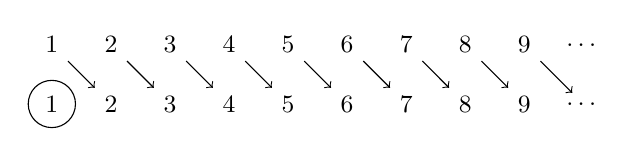
\begin{tikzpicture}[scale = .75]
		\foreach \x in {1, 2, 3, 4, 5, 6, 7, 8, 9}
		{
			\node (\x a) at (\x, 1) {\small{\x}};
			\node (\x b) at (\x, 2) {\small{\x}};
		}
		\node (dotsa) at (10, 1) {\small{\ldots}};
		\node (dotsb) at (10, 2) {\small{\ldots}};
		\draw[->] (1b)--(2a);
		\draw[->] (2b)--(3a);
		\draw[->] (3b)--(4a);
		\draw[->] (4b)--(5a);
		\draw[->] (5b)--(6a);
		\draw[->] (6b)--(7a);
		\draw[->] (7b)--(8a);
		\draw[->] (8b)--(9a);
		\draw[->] (9b)--(dotsa);
		\draw (1,1) circle (.4);
		\end{tikzpicture}
	\end{center}
	(\citealt[730]{EwaldSieg2013}માં પ્રકાશિત; અમારો અનુવાદ)
\end{quote}
નિર્ણાયક મુદ્દો એ છે કે હિલ્બર્ટની હોટેલમાં અનંત ઓરડાઓ છે; અને આમ
કહેવાનો અર્થ શું થાય તેની વ્યાખ્યા તરીકે આપણે તેમની સમજૂતી લઈ શકીએ.
ખરેખર, ડેડેકિન્ડનો અભિગમ પણ આ જ હતો (અલબત્ત, અહીં ભારે કાળવિપર્યય
સાથે રજૂ કર્યો છે; ડેડેકિન્ડની વ્યાખ્યા \citeyear{Dedekind1888}ની છે):

\begin{defn}\ollabel{defn:DedekindInfinite}
ગણ $A$ \emph{ડેડેકિન્ડ-અનંત} હોય જો અને માત્ર જો $A$થી $A$ના કોઈ
ઉચિત ઉપગણમાં એક-એક વિધેય હોય. એટલે કે, કોઈ $o \in A$ અને
એક-એક વિધેય $f \colon A \to A$ એવાં હોય કે $o \notin \ran{f}$.
\end{defn}




\olfileid{sfr}{infinite}{dedekind}
\olsection{ડેડેકિન્ડ બીજગણિતો}

આપણે પ્રાકૃતિક સંખ્યાઓ માત્ર અનંત હોય એટલું જ નથી માગતા; આપણે એમ પણ
માગીએ છીએ કે તેમને અમુક (બૈજિક) ગુણધર્મો હોય: સરવાળા, ગુણાકાર વગેરે
હેઠળ તેમનો વ્યવહાર સુસંગત હોવો જોઈએ.

ડેડેકિન્ડનો વિચાર \emph{અનુગામી વિધેય}ના ખ્યાલને મૂળભૂત માનવાનો અને
પછી નીચેના ગુણધર્મો ધરાવતી સંખ્યાઓ તરીકે તેમનું લક્ષણ આપવાનો હતો:
\begin{enumerate}
	\item એવી સંખ્યા $0$ છે જે કોઈ પણ સંખ્યાની અનુગામી નથી
	\\અર્થાત્, $0 \notin \ran{s}$
	\\અર્થાત્, $\forall x\ s(x) \neq 0$
	\item ભિન્ન સંખ્યાઓના અનુગામીઓ ભિન્ન હોય છે
	\\અર્થાત્, $s$ એ એક-એક વિધેય છે
	\\અર્થાત્, $\forall x \forall y (s(x) = s(y) \lif x = y)$
	\item\ollabel{repeatedapplication} દરેક સંખ્યા $0$ પર અનુગામી
	વિધેય વારંવાર લગાડવાથી મળે છે.
\end{enumerate}
પહેલી બે શરતોને પ્રથમ-ક્રમ તર્કશાસ્ત્રથી સહેલાઈથી સંભાળી શકાય છે
(ઉપર જુઓ). પરંતુ માત્ર પ્રથમ-ક્રમ તર્કશાસ્ત્રથી
\olref{repeatedapplication}ને સંભાળી શકાતી નથી. ડેડેકિન્ડની સફળતા
શરત \olref{repeatedapplication}ને ગણસૈદ્ધાંતિક રીતે આ પ્રમાણે ફરી
ઘડવામાં હતી:
\begin{enumerate}
	\item[3$'$.] પ્રાકૃતિક સંખ્યાઓ એવો નાનામાં નાનો ગણ છે જે
	\emph{અનુગામી વિધેય હેઠળ સંવૃત} છે: એટલે કે, ગણના કોઈ પણ
	ઘટક પર $s$ લગાડીએ તો ગણનો બીજો ઘટક મળે છે.
\end{enumerate}
પરંતુ આ વાત આપણે ધીમે ધીમે પૂરેપૂરી સ્પષ્ટ કરવી પડશે.

\begin{defn}\ollabel{Closure}
	દરેક વિધેય $f \colon A \to A$ માટે ગણ $X \subseteq A$ એ
	$f$-\emph{સંવૃત} છે {iff} $(\forall x \in X)f(x) \in X$.
	હવે દરેક $o \in A$ માટે વ્યાખ્યા કરીએ:
	$$\closureofunder{f}{o} = \bigcap\Setabs{X}{o \in X\text{ અને }X
\text{ એ $f$-સંવૃત છે}}$$
\end{defn}
\sourcecorrection{OLINF-001}{મૂળની \texttt{dedekind-algebra.tex},
પંક્તિઓ 40--64માં સંવરણની વ્યાખ્યા કોઈ પણ $f$ અને $o$ માટે અપાઈ
છે, પછીના લેમામાં $A$ને બાંધ્યા વિના $o\in A$ લખાયું છે, અને
સાબિતીમાં $\ran{f}\cup\{o\}$ એ $f$-સંવૃત હોવાનો ઉપયોગ થાય છે.
આ દલીલને જરૂરી અને પછીના બધા ઉપયોગો સાથે સુસંગત એવી ધારણા
$f\colon A\to A$, $X\subseteq A$ અને $o\in A$ અહીં સ્પષ્ટ કરી છે.}

આમ $\closureofunder{f}{o}$ એ એવા બધા $f$-સંવૃત ગણોનો છેદ છે
જેમનો ઘટક~$o$ છે. તેથી સહજ રીતે,
$\closureofunder{f}{o}$ એ ઘટક તરીકે $o$ ધરાવતો
\emph{નાનામાં નાનો} $f$-સંવૃત ગણ છે. આગળનું પરિણામ આ સહજ વિચારને
ચોક્કસ બનાવે છે;
\begin{lem}\ollabel{closureproperties}
	દરેક વિધેય $f \colon A \to A$ અને દરેક $o \in A$ માટે:
	\begin{enumerate}
		\item\ollabel{closurehaselem} $o \in \closureofunder{f}{o}$; અને
		\item\ollabel{closureclosed} $\closureofunder{f}{o}$ એ $f$-સંવૃત છે; અને
		\item\ollabel{closuresmallest} જો $X$ એ $f$-સંવૃત હોય અને $o \in
		X$, તો $\closureofunder{f}{o} \subseteq X$.
	\end{enumerate}
\end{lem}

\begin{proof}
નોંધો કે ઘટક તરીકે $o$ ધરાવતો ઓછામાં ઓછો એક $f$-સંવૃત ગણ
છે, એટલે કે $\ran{f}\cup \{o\}$. તેથી આવા \emph{બધા} ગણોનો છેદ
$\closureofunder{f}{o}$ અસ્તિત્વ ધરાવે છે. હવે આપણે
\olref{closurehaselem}--\olref{closuresmallest} તપાસવાં છે.

\olref{closurehaselem} અંગે: $o \in \closureofunder{f}{o}$, કારણ કે
તે એવા ગણોનો છેદ છે જેમના દરેકનો ઘટક~$o$ છે.

\olref{closureclosed} અંગે: ધારો કે $x \in \closureofunder{f}{o}$.
તેથી જો $o \in X$ અને $X$ એ $f$-સંવૃત હોય, તો $x \in X$; અને
$X$ એ $f$-સંવૃત હોવાથી હવે $f(x) \in X$. તેથી
$f(x) \in \closureofunder{f}{o}$.

\olref{closuresmallest} અંગે: સામાન્ય રીતે, જો $X \in C$ હોય, તો
$\bigcap C \subseteq X$.
\end{proof}

આનો ઉપયોગ કરીને આપણે કહી શકીએ:

\begin{defn}
\emph{ડેડેકિન્ડ બીજગણિત} એટલે ગણ $A$, વિધેય $f \colon A \to A$
અને કોઈ $o \in A$ એવાં કે:
	\begin{enumerate}
		\item \ollabel{ded:proper} $o \notin \ran{f}$
		\item \ollabel{ded:injection} $f$ એ એક-એક વિધેય છે
		\item \ollabel{ded:closure} $A = \closureofunder{f}{o}$
	\end{enumerate}
\end{defn}

$A = \closureofunder{f}{o}$ હોવાથી આપણું પહેલાનું પરિણામ જણાવે છે કે
$A$ એ ઘટક તરીકે $o$ ધરાવતો નાનામાં નાનો $f$-સંવૃત ગણ છે.
ડેડેકિન્ડ બીજગણિત સ્પષ્ટપણે ડેડેકિન્ડ-અનંત છે; વ્યાખ્યાની કલમો
\olref{ded:proper} અને \olref{ded:injection} જ જુઓ. પરંતુ વધુ રસપ્રદ
હકીકત એ છે કે કોઈ પણ ડેડેકિન્ડ-અનંત ગણને ડેડેકિન્ડ બીજગણિતમાં ફેરવી
શકાય છે.

\begin{thm}\ollabel{thm:DedekindInfiniteAlgebra}
જો કોઈ ડેડેકિન્ડ-અનંત ગણ હોય, તો કોઈ ડેડેકિન્ડ બીજગણિત હોય છે.
\end{thm}

\begin{proof}
ધારો કે $D$ ડેડેકિન્ડ-અનંત છે. તેથી એક-એક વિધેય $g \colon D \to
D$ અને ઘટક $o \in D \setminus \ran{g}$ છે. હવે $A =
\closureofunder{g}{o}$ લો; \olref{closureproperties} મુજબ $A$
અસ્તિત્વ ધરાવે છે અને $o \in A$. $f = \funrestrictionto{g}{A}$ લો.
$A, f, o$ મળીને ડેડેકિન્ડ બીજગણિત રચે છે તે આપણે બતાવીશું.

\olref{ded:proper} અંગે: $o \notin \ran{g}$ અને $\ran{f}
\subseteq \ran{g}$ હોવાથી $o\notin \ran{f}$.

\olref{ded:injection} અંગે: $g$ એ $D$ પર એક-એક વિધેય છે; તેથી
$f \subseteq g$ પણ એક-એક વિધેય જ હોય.

\olref{ded:closure} અંગે: \olref{closureproperties} મુજબ $A$ એ
$g$-સંવૃત છે; તેથી ખાસ કરીને $A$ એ $f$-સંવૃત છે. આમ
$\closureofunder{f}{o} \subseteq A$ એ \olref{closureproperties}થી મળે
છે. વળી $\closureofunder{f}{o}$ એ $f$-સંવૃત છે અને
$f = \funrestrictionto{g}{A}$ હોવાથી $\closureofunder{f}{o}$ એ
$g$-સંવૃત છે. તેથી \olref{closureproperties} મુજબ
$A \subseteq \closureofunder{f}{o}$.
\end{proof}




\olfileid{sfr}{infinite}{induction}
\olsection[ગાણિતિક અનુમાન]{ડેડેકિન્ડ બીજગણિતો અને ગાણિતિક અનુમાન}

હવે નિર્ણાયક વાત એ છે કે ડેડેકિન્ડ બીજગણિત---ખરેખર, \emph{કોઈ પણ}
ડેડેકિન્ડ બીજગણિત---પ્રાકૃતિક સંખ્યાઓના અવેજ તરીકે કામ કરશે. આ નીચેના
સરળ પરિણામને આભારી છે:

\begin{thm}[ગાણિતિક અનુમાન]\ollabel{thm:dedinfiniteinduction}
ધારો કે $N, s, o$ મળીને ડેડેકિન્ડ બીજગણિત રચે છે. ત્યારે દરેક ગણ $X$ માટે:
	\begin{center}
		જો $o \in X$ અને $(\forall {n} \in N \cap X){s}({n}) \in X$, {તો} $N \subseteq X$.
	\end{center}
\end{thm}

\begin{proof}
ડેડેકિન્ડ બીજગણિતની વ્યાખ્યા મુજબ $N = \closureofunder{s}{o}$.
હવે જો ${o} \in X$ અને $(\forall {n} \in N)(n \in X \lif
{s}({n}) \in X)$ બંને હોય, તો $N = \closureofunder{s}{o} \subseteq X$.
\end{proof}

ગાણિતિક અનુમાન પ્રાકૃતિક સંખ્યાઓનું વિશિષ્ટ લક્ષણ હોવાથી મુદ્દો આ છે.
કોઈ પણ ડેડેકિન્ડ-અનંત ગણ આપેલો હોય, તો આપણે ડેડેકિન્ડ બીજગણિત રચીને
તેને પ્રાકૃતિક સંખ્યાઓના અવેજ તરીકે વાપરી શકીએ છીએ.

કબૂલ કે \olref{thm:dedinfiniteinduction}માં અનુમાનને
\emph{ગણસૈદ્ધાંતિક} પદોમાં ઘડ્યું છે. પરંતુ આ સિદ્ધાંતને આપણને વધુ
પરિચિત હોય એવાં પદોમાં સહેલાઈથી મૂકી શકીએ છીએ:

\begin{cor}\ollabel{natinductionschema}
ધારો કે $N, s, o$ મળીને ડેડેકિન્ડ બીજગણિત રચે છે. ત્યારે પ્રાચલો
હોઈ શકે એવા દરેક સૂત્ર $\phi(x)$ માટે:
\begin{center}
	જો $\phi(o)$ અને $(\forall {n} \in N)(\phi(n)\lif
	\phi({s}({n})))$, {તો} $(\forall n \in N)\phi(n)$.
\end{center}
\end{cor}

\begin{proof}
$X = \Setabs{n \in N}{\phi(n)}$ લો અને હવે
\olref{thm:dedinfiniteinduction} વાપરો.
\end{proof}

આ પરિણામમાં આપણે કોઈ સૂત્ર ``પ્રાચલો ધરાવે છે'' એવું કહ્યું. તેનો
આશરે અર્થ એ છે કે કોઈ પણ વસ્તુઓ $c_1, \ldots, c_k$ માટે આપણે
$\phi(x, c_1, \ldots, c_k)$ સાથે કામ કરી શકીએ છીએ. વધુ ચોક્કસ રીતે,
``પ્રાચલો''નો ઉલ્લેખ કર્યા વિના પરિણામ આ પ્રમાણે કહી શકાય. દરેક સૂત્ર
$\phi(x, v_1, \ldots, v_k)$ માટે, જેના બધા મુક્ત ચલો દર્શાવેલા છે,
આપણી પાસે છે:
	\begin{align*}
			\forall v_1 \ldots \forall v_k((&\phi(o, v_1,\ldots, v_k) \land {}\\
			&	(\forall x \in N)(\phi(x,v_1, \ldots, v_k) \lif \phi(s(x), v_1,\ldots, v_k))) \lif {}\\
			&\hspace{3em} (\forall x \in N)\phi(x, v_1,\ldots, v_k))
	\end{align*}
સ્પષ્ટ છે કે ``પ્રાચલો ધરાવે છે'' એવો વાક્યપ્રયોગ વાંચવાનું ઘણું સરળ
બનાવી શકે છે. (\olref[sth][][]{part}માં આપણે આ રીત ઘણી વાર વાપરીશું.)

ડેડેકિન્ડ બીજગણિતો તરફ પાછા ફરીએ: કોઈ પણ ડેડેકિન્ડ બીજગણિત આપેલું
હોય, તો આપણે સરવાળા, ગુણાકાર અને ઘાતની ક્રિયાનાં સામાન્ય અંકગણિતીય
વિધેયો પણ વ્યાખ્યાયિત કરી શકીએ છીએ. જોકે આ બાબત તુચ્છ નથી અને તેમાં
\emph{પુનરાવર્તી વ્યાખ્યા}ની રીત વપરાય છે. આ રીતનો પરિચય અને ઔચિત્ય
આપણે ઘણું પાછળ, અને વધુ વ્યાપક સંદર્ભમાં આપીશું. (રસ ધરાવતા વાચકો
\olref[sth][ord-arithmetic][]{chap} પછી આ મુદ્દો ફરી જોઈ શકે, અથવા
\citealt[pp.~95--8]{Potter2004} જેવી વૈકલ્પિક રજૂઆત વાંચી શકે.) પરંતુ
જ્યાં $N, s, o$ મળીને ડેડેકિન્ડ બીજગણિત રચે છે, ત્યાં અંતે આપણે નીચે
પ્રમાણે ઠરાવી શકીશું:
\begin{align*}
	{a} + {o} &= {a} & & & {a} \times {o} &= {o} & & & {a}^{o} &= s(o)\\
{a} + {s}({b}) &= {s}({a}+{b}) &&& {a} \times {s}({b}) &= ({a}\times {b}) + {a}  & & & {a}^{{s}({b})} &= {a}^{b} \times {a}
\end{align*}
અને તે આશા મુજબ વર્તે છે એવું બતાવી શકીશું.




\olfileid{sfr}{infinite}{dedekindsproof}

\olsection[ડેડેકિન્ડની ``સાબિતી'']{અનંત ગણના અસ્તિત્વની
ડેડેકિન્ડની ``સાબિતી''}

આ પ્રકરણમાં આપણે ડેડેકિન્ડ બીજગણિતો વડે પ્રાકૃતિક સંખ્યાઓની
ગણસૈદ્ધાંતિક રજૂઆત કરી છે. \olref[arith][ref]{sec}માં આપણે
વિશ્લેષણના અંકગણિતીકરણના (બીજી બાબતો સાથે) તાત્ત્વિક મહત્ત્વ પર
વિચાર કર્યો હતો. હવે આપણે અહીં જે સિદ્ધ કર્યું છે તેના મહત્ત્વ પર
વિચાર કરવો જોઈએ.

સમગ્ર \olref[sfr][arith][]{chap}માં આપણે પ્રાકૃતિક સંખ્યાઓને આપેલી
માની અને તેમનો ઉપયોગ કરીને પૂર્ણાંકો, સંમેય સંખ્યાઓ અને વાસ્તવિક
સંખ્યાઓની સ્પષ્ટ રચના કરી. આ પ્રકરણમાં આપણે પ્રાકૃતિક સંખ્યાઓની સ્પષ્ટ
રચના આપી નથી. આપણે માત્ર એટલું બતાવ્યું છે કે \emph{કોઈ પણ
ડેડેકિન્ડ-અનંત ગણ આપેલો હોય}, તો એવો ગણ વ્યાખ્યાયિત કરી શકાય છે જે
આપણે~$\Nat$ પાસે ઇચ્છીએ છીએ તેવો જ વ્યવહાર કરશે.

તેથી \emph{કઈ વસ્તુઓ પ્રાકૃતિક સંખ્યાઓ છે} એવા અધિભૌતિક પ્રશ્નનો
જવાબ આપ્યો હોવાનો દાવો આપણે કરી શકતા નથી. પરંતુ એ સારી વાત છે. છેવટે,
\olref[sfr][arith][ref]{sec}માં આપણે ભાર મૂક્યો હતો કે
$\Real$ને ડેડેકિન્ડ કાપોના ગણ તરીકે આપેલી વ્યાખ્યાને અનુકૂળ ઠરાવને
બદલે \emph{શોધ} માનવી ખોટી છે. નિર્ણાયક અવલોકન એ છે કે ડેડેકિન્ડ
કાપો વાસ્તવિક સંખ્યાઓના મુખ્ય ગણિતીય ગુણધર્મોને મૂર્ત કરે છે. અહીં
પણ એવું જ છે: \emph{કોઈ પણ} ડેડેકિન્ડ બીજગણિત પ્રાકૃતિક સંખ્યાઓના
મુખ્ય ગણિતીય ગુણધર્મોને મૂર્ત કરે છે. (ખરેખર, બધા ડેડેકિન્ડ બીજગણિતો
\emph{એકરૂપ} છે એવું સાબિત કરીને ડેડેકિન્ડે આ મુદ્દો દૃઢ કર્યો
(\citeyear[Theorems
132--3]{Dedekind1888}). તેથી ઘણા સમકાલીન
``સંરચનાવાદીઓ'' ડેડેકિન્ડને પોતાના પુરોગામી ગણે છે તેમાં નવાઈ નથી.)

 વળી, આપણે બતાવ્યું છે કે પ્રાકૃતિક સંખ્યાઓના સિદ્ધાંતને સહજ સરળ
 ગણસિદ્ધાંતમાં કેવી રીતે સ્થાપિત કરવો. આ ગણસિદ્ધાંત હજી ખાસ્સો
 અનૌપચારિક છે, પરંતુ તેમાં પ્રાકૃતિક સંખ્યાઓ આપેલી છે એવું (દેખીતી
 રીતે) માનવામાં આવતું નથી. તેથી આપણે ડેડેકિન્ડના પોતાના મહત્ત્વાકાંક્ષી
 યોજનાને સાકાર કરવાની દિશામાં હોઈ શકીએ છીએ; તેમણે તેને આ પ્રમાણે
 સમજાવી હતી:
\begin{quote}
	વિજ્ઞાનમાં જે બાબતની સાબિતી શક્ય હોય તે સાબિતી વિના માનવી ન જોઈએ.
	આ માગ વાજબી લાગતી હોવા છતાં, સૌથી સરળ વિજ્ઞાનનો પાયો નાખવાની
	અત્યંત નવીન પદ્ધતિઓમાં પણ તે સંતોષાઈ છે એમ હું માની શકતો નથી;
	અર્થાત્ તર્કશાસ્ત્રનો એ ભાગ જે સંખ્યાઓના સિદ્ધાંત સાથે સંબંધિત છે.
	અંકગણિત (બીજગણિત, વિશ્લેષણ) માત્ર તર્કશાસ્ત્રનો ભાગ છે એમ કહેતાં
	મારો આશય એ છે કે સંખ્યાનો ખ્યાલ અવકાશ અને સમયની કલ્પનાઓ કે
	અંતઃપ્રજ્ઞાથી સંપૂર્ણપણે સ્વતંત્ર છે---હું તેને વિચારના શુદ્ધ
	નિયમોની સીધી નિષ્પત્તિ માનું છું.
	\citep[preface]{Dedekind1888}
\end{quote}
ડેડેકિન્ડનો સાહસિક વિચાર આ છે. માત્ર (સહજ) ગણસિદ્ધાંત વાપરીને
પ્રાકૃતિક સંખ્યાઓ કેવી રીતે રચવી તે આપણે હમણાં જ બતાવ્યું.
\olref[sfr][arith][]{chap}માં પ્રાકૃતિક સંખ્યાઓ અને થોડો ગણસિદ્ધાંત
આપેલાં હોય ત્યારે વાસ્તવિક સંખ્યાઓ કેવી રીતે રચવી તે જોયું. તેથી કદાચ
``અંકગણિત (બીજગણિત, વિશ્લેષણ)'' એ ``માત્ર તર્કશાસ્ત્રનો ભાગ'' ઠરે
(ડેડેકિન્ડના ``તર્કશાસ્ત્ર'' શબ્દના વિસ્તૃત અર્થમાં).

વિચાર આ છે. પરંતુ જરા થોભો. ડેડેકિન્ડ બીજગણિતની આપણી રચના
(પ્રાકૃતિક સંખ્યાઓનો આપણો અવેજ) ડેડેકિન્ડ-અનંત ગણના અસ્તિત્વ પર
આધારિત છે. (ફરી \olref[sfr][infinite][dedekind]{thm:DedekindInfiniteAlgebra}
જુઓ.) જો ``તર્કશાસ્ત્ર'' અથવા ``વિચારના શુદ્ધ નિયમો'' વડે
ડેડેકિન્ડ-અનંત ગણનું અસ્તિત્વ સ્થાપિત ન કરી શકાય, તો યોજના અટકી જાય છે.

તો શું ``વિચારના શુદ્ધ નિયમો'' વડે ડેડેકિન્ડ-અનંત ગણનું અસ્તિત્વ
સ્થાપિત કરી શકાય? ડેડેકિન્ડનો પ્રયાસ આ હતો:
\begin{quote}
  મારા પોતાના વિચારોનું ક્ષેત્ર, એટલે કે મારા વિચારના વિષય બની શકે
  એવી બધી વસ્તુઓની સમગ્રતા $S$, અનંત છે. કારણ કે જો $s$ એ $S$નો
  ઘટક દર્શાવે, તો $s$ મારા વિચારનો વિષય બની શકે છે એવો વિચાર $s'$ પણ
  પોતે $S$નો ઘટક છે. જો આપણે તેને ઘટક~$s$ના પ્રતિબિંબ $\phi(s)$ તરીકે
  લઈએ, તો \dots~$S$ [ડેડેકિન્ડના અર્થમાં] અનંત છે, જે સાબિત કરવાનું હતું.
	\citep[\S66]{Dedekind1888}
\end{quote}
મોટાભાગે અત્યંત ચુસ્ત ગણિતીય સાબિતીઓથી બનેલા પુસ્તકની વચ્ચે આવી વાત
મળે તે ખરેખર આશ્ચર્યજનક છે. બે ટિપ્પણીઓ કરવા જેવી છે.

પહેલી: આ ``સાબિતી''માં આજે આપણે જેને ``ગણિતીય'' સ્વરૂપ કહીએ એવું
ભાગ્યે જ કંઈ છે. તેમાં મનોવૈજ્ઞાનિક વસ્તુઓ (વિચારો)ની વાત થાય છે, અને
તે પણ માત્ર \emph{સંભવિત} વિચારોની.

બીજી: ઓછામાં ઓછું આપણે ડેડેકિન્ડ બીજગણિતો જે રીતે રજૂ કર્યાં છે તે
દૃષ્ટિએ, આ ``સાબિતી''માં સીધી તકનીકી ખામી છે. ડેડેકિન્ડની દલીલ સફળ
હોય તો તે માત્ર એટલું સ્થાપિત કરે છે કે અનંત સંખ્યામાં વસ્તુઓ છે
(ખાસ કરીને, અનંત સંખ્યામાં વિચારો). પરંતુ ડેડેકિન્ડે આપણને એ માનવાનું
કારણ પણ આપવું પડે કે~$S$ એ અનંત ઘણા ઘટકો ધરાવતો એક જ
\emph{ગણ} છે; $S$ને માત્ર \emph{કેટલીક વસ્તુઓ} (બહુવચનમાં) માનવું
યોગ્ય નથી.

ડેડેકિન્ડે અહીં ખામી જોઈ નહીં તે હકીકત કદાચ સૂચવે છે કે
``સમગ્રતા'' શબ્દનો તેમનો ઉપયોગ \emph{ગણ} શબ્દના \emph{આપણા} ઉપયોગને
ચોક્કસપણે અનુસરતો નથી.\footnote{ખરેખર, એવું નહોતું માનવાનાં બીજાં
કારણો પણ છે; \citet[p.~23]{Potter2004} જુઓ.} પરંતુ આમાં બહુ નવાઈ નથી.
છેલ્લાં બે પ્રકરણમાં આપણે હાથ ધરેલો પ્રકલ્પ---પ્રાકૃતિક સંખ્યાઓની
``રચના'', અને તેમાંથી પૂર્ણાંકો, વાસ્તવિક સંખ્યાઓ અને સંમેય સંખ્યાઓની
``રચના''---સંપૂર્ણપણે સહજ રીતે કર્યો છે. કયા ગણો અસ્તિત્વ ધરાવે છે અને
ક્યારે ધરાવે છે તે વિશે ઘણા સામાન્ય સિદ્ધાંતો મૂક્યા વિના, જરૂર પડતી
ગઈ તેમ આ ગણ અથવા તે ગણ માની લીધા છે. પરંતુ આપણે જાણીએ છીએ કે
\emph{કેટલાક} સામાન્ય સિદ્ધાંતો જરૂરી છે; નહિતર આપણે રસેલના
વિરોધાભાસમાં ફસાઈ જઈશું.

 હવે આપણી સહજતાની મર્યાદા છોડવાનો સમય આવી ગયો છે.




\olfileid{sfr}{infinite}{card-sb}

\olsection{પરિશિષ્ટ: શ્રેડર--બર્નસ્ટાઇનની સાબિતી}

સહજ ગણસિદ્ધાંત છોડીએ તે પહેલાં એક છેલ્લી સહજ (પણ સુવિકસિત!) સાબિતી
વિચારવાની બાકી છે. આ શ્રેડર--બર્નસ્ટાઇન
(\olref[sfr][siz][sb]{thm:schroder-bernstein})ની સાબિતી છે: જો
$\cardle{A}{B}$ અને $\cardle{B}{A}$ હોય, તો $\cardeq{A}{B}$; એટલે કે,
એક-એક વિધેયો $f \colon A \to B$ અને $g \colon B \to A$ આપેલાં હોય,
તો એક-એક વ્યાપ્ત વિધેય $h \colon A \to B$ હોય છે.

આ પ્રકરણમાં આપણે ડેડેકિન્ડના \emph{સંવરણો}ના ખ્યાલને અનુસર્યા છીએ.
ખરેખર, ડેડેકિન્ડે આ ખ્યાલ વાપરીને શ્રેડર--બર્નસ્ટાઇનની એક સુંદર
સાબિતી આપી હતી અને આપણે તેને અહીં રજૂ કરીશું. અહીંની સાબિતી
\citet[pp.~157--8]{Potter2004}ને નજીકથી અનુસરે છે; ત્યાં થોડું જુદું
પણ મૂળભૂત રીતે સરખું નિરૂપણ મળશે. થોડું ગૂગલમાં
શોધવાથી પણ ખાતરી થશે કે---$\sqrt{2}$ની અસંમેયતા જેવું---આ એવું પ્રમેય
છે જેની \emph{ઘણી} રસપ્રદ અને જુદી સાબિતીઓ છે.

\olref[sfr][infinite][dedekind]{Closure} જેવી જ સંજ્ઞા વાપરીને,
દરેક ગણ $B$ અને વિધેય~$f$ માટે લો:
\[
\Closureofunder{f}{B} = \bigcap \Setabs{X}{B \subseteq X
\text{ અને $X$ એ $f$-સંવૃત છે}}
\]
આ રીતે વ્યાખ્યાયિત $\Closureofunder{f}{B}$ એ $B$ને સમાવતો નાનામાં
નાનો $f$-સંવૃત ગણ છે, એ અર્થમાં કે:

\begin{lem}\ollabel{Closureprops}
	દરેક વિધેય $f$ અને દરેક $B$ માટે:
	\begin{enumerate}
		\item\ollabel{Closurehaselem} $B \subseteq \Closureofunder{f}{B}$; અને
		\item\ollabel{Closureclosed} $\Closureofunder{f}{B}$ એ $f$-સંવૃત છે; અને
		\item\ollabel{Closuresmallest} જો $X$ એ $f$-સંવૃત હોય અને $B
		\subseteq X$, તો $\Closureofunder{f}{B} \subseteq X$.
	\end{enumerate}
\end{lem}

\begin{proof}
બરાબર \olref[sfr][infinite][dedekind]{closureproperties}ની જેમ.
\end{proof}

શ્રેડર--બર્નસ્ટાઇન સુધી પહોંચવા માટે એક છેલ્લી હકીકત જોઈએ:

\begin{prop}\ollabel{sbhelper}
જો $A \subseteq B \subseteq C$ અને $A \approx C$ હોય, તો
$\cardeq{A}{B}$ અને $\cardeq{B}{C}$.
\end{prop}
\sourcecorrection{OLINF-002}{પછીની સ્વતંત્ર સમીક્ષાએ આ નોંધનું
મૂળ-ખામી તરીકેનું અગાઉનું વર્ગીકરણ પાછું ખેંચ્યું છે. મૂળની
\texttt{card-sb.tex}, પંક્તિ~52નું $\cardeq{\cardeq{A}{B}}{C}$,
\texttt{\string\cardeq}ની બે-દલીલી વ્યાખ્યા પ્રમાણે,
$A \approx B \approx C$માં વિસ્તરે છે; તેથી તેમાં દલીલસંખ્યાની કે
ગણિતીય ખામી નથી. ગુજરાતી મુખ્ય પાઠમાં સાબિતી સ્થાપિત કરતી બે
સમાનતાઓને સ્પષ્ટ સંયોજન રૂપે જાળવી છે. આ મૂળ નિષ્કર્ષની સમકક્ષ
રજૂઆત છે, મૂળની સુધારણા નહીં.}

\begin{proof}
એક-એક વ્યાપ્ત વિધેય $f \colon C \to A$ આપેલું હોય, ત્યારે $F =
\Closureofunder{f}{C \setminus B}$ લો અને પ્રદેશ $C$ ધરાવતું વિધેય
$g$ આ પ્રમાણે વ્યાખ્યાયિત કરો:
\[
	g(x) =
	\begin{cases}
			f(x) &\text{જો $x \in F$}\\
			x & \text{અન્યથા}
		\end{cases}
\]
$g$ એ $C \to B$નું એક-એક વ્યાપ્ત વિધેય છે તે આપણે બતાવીશું; તેના પરથી
$\comp{f^{-1}}{g} \colon A \to B$ એ એક-એક વ્યાપ્ત વિધેય છે એવું મળશે અને
સાબિતી પૂરી થશે.

પહેલો દાવો એ છે કે જો $x \in F$ પણ $y\notin F$ હોય, તો
$g(x) \neq g(y)$. વિરોધાભાસ મેળવવા ઊલટું ધારો; ત્યારે
$y = g(y) = g(x) = f(x)$. \olref{Closureprops} મુજબ $F$ એ
$f$-સંવૃત છે અને $x \in F$ હોવાથી $y = f(x) \in F$, જે વિરોધાભાસ છે.

હવે ધારો કે $g(x) = g(y)$. તેથી ઉપરના દાવાથી $x \in F$ જો અને માત્ર
જો $y \in F$. જો $x, y \in F$, તો $f(x) = g (x) = g(y) = f(y)$;
અને $f$ એ એક-એક વ્યાપ્ત વિધેય હોવાથી $x = y$. જો $x, y \notin F$, તો
$x = g(x) = g(y) = y$. તેથી $g$ એ એક-એક વિધેય છે.

હવે માત્ર $\ran{g} = B$ બતાવવાનું બાકી છે. તેથી $x \in B \subseteq C$
નિશ્ચિત કરો. જો $x \notin F$, તો $g(x) = x$. જો $x \in F$, તો કોઈ
$y \in F$ માટે $x = f(y)$; કારણ કે નહિતર $F \setminus \{x\}$ એ
$f$-સંવૃત હોત અને $C\setminus B$ને સમાવતો હોત, જે
\olref{Closureprops}થી અશક્ય છે. હવે $g(y) = f(y) = x$.
\end{proof}

છેલ્લે મુખ્ય પરિણામની સાબિતી આ રહી. યાદ કરો કે વિધેય $h$ અને ગણ $D$
આપેલાં હોય ત્યારે આપણે $\funimage{h}{D} = \Setabs{h(x)}{x
\in D}$ વ્યાખ્યાયિત કરીએ છીએ.

\begin{proof}[શ્રેડર--બર્નસ્ટાઇનની સાબિતી] ધારો કે $f \colon A \to B$
અને $g \colon B \to A$ એ એક-એક વિધેયો છે. $\funimage{f}{A}
\subseteq B$ હોવાથી $\funimage{g}{\funimage{f}{A}} \subseteq
g[B] \subseteq A$. વળી, $g$ અને $f$ બંને એક-એક હોવાથી
$\comp{f}{g} \colon A \to \funimage{g}{\funimage{f}{A}}$ પણ
એક-એક વિધેય છે; અને ખરેખર, તેનો સહપ્રદેશ જે રીતે વ્યાખ્યાયિત કર્યો
છે તે પરથી $\comp{f}{g}$ એ એક-એક વ્યાપ્ત વિધેય છે. તેથી
$\cardeq{\funimage{g}{\funimage{f}{A}}}{A}$ અને આમ
\olref{sbhelper} મુજબ કોઈ એક-એક વ્યાપ્ત વિધેય $h \colon A \to
\funimage{g}{B}$ છે. વળી, $g^{-1}$ એ એક-એક વ્યાપ્ત વિધેય
$\funimage{g}{B} \to B$ છે. તેથી $\comp{h}{g^{-1}} \colon A \to B$
એ એક-એક વ્યાપ્ત વિધેય છે.
\end{proof}



\part{વિધાનાત્મક તર્કશાસ્ત્ર}


\olfileid{pl}{syn}{int}

\olsection{પરિચય}

વિધાનાત્મક તર્કશાસ્ત્રમાં $\lnot$, $\land$, $\lor$, $\lif$ અને
$\liff$ એ વિધાનાત્મક સંયોજકો વડે વિધાનચલોમાંથી
બનાવેલાં સૂત્રોનો અભ્યાસ થાય છે. સહજ રીતે કહીએ તો,
વિધાનચલ~$p$ સત્ય કે અસત્ય હોઈ શકે એવા વાક્ય
અથવા વિધાનને રજૂ કરે છે. સૂત્રમાંના વિધાનચલનું
``સત્યમૂલ્ય'' નક્કી થાય એટલે વિધાનાત્મક સંયોજકો વડે તેમાંથી બનાવેલાં
સૂત્રોનું સત્યમૂલ્ય પણ નક્કી થાય છે. આપણે
વિધાનાત્મક તર્કશાસ્ત્રને \emph{સત્યતાફલનલક્ષી} કહીએ છીએ, કારણ કે તેનો
અર્થવિચાર સત્યમૂલ્યોનાં વિધેયો વડે અપાય છે. ખાસ કરીને, વિધાનાત્મક
તર્કશાસ્ત્રમાં સત્ય અને અસત્યના બીજા કોઈ નિર્ધારણને ધ્યાનમાં લેતા નથી;
દાખલા તરીકે, કોઈ વાત માત્ર સંજોગવશાત્ સત્ય હોવાને બદલે અનિવાર્યપણે
સત્ય છે કે નહિ, તે સત્ય છે એવું જાણીતું છે કે નહિ, અથવા તે હમણાં
સત્ય છે કે પહેલાં સત્ય હતી કે પછી સત્ય થશે. આપણે માત્ર સત્ય
($\True$) અને અસત્ય ($\False$) એ બે સત્યમૂલ્યો લઈએ છીએ; એટલે કોઈ
કથન ન તો સત્ય ન તો અસત્ય, અથવા માત્ર અડધું સત્ય હોઈ શકે એવી શક્યતા
ચર્ચામાંથી બહાર રાખીએ છીએ. વળી, આપણે માત્ર એવા સંયોજકો પર ધ્યાન
આપીએ છીએ જેમનાથી બનેલા સૂત્રનું સત્યમૂલ્ય તેના ભાગોનાં
સત્યમૂલ્યો વડે સંપૂર્ણપણે નક્કી થાય છે (અને, માનો કે, તેના અર્થ વડે
નહિ). ખાસ કરીને, અંગ્રેજી ભાષાનાં શરતી વાક્યોનું સત્યમૂલ્ય આ અર્થમાં
સત્યતાફલનલક્ષી છે કે નહિ તે વિવાદાસ્પદ છે. સત્યમૂલ્યલક્ષી પ્રેરણ
$\lif$ એવું છે; બીજા તર્કશાસ્ત્રો સત્યતાફલનલક્ષી ન હોય એવાં શરતી
વિધાનોનો અભ્યાસ કરે છે.

સત્યતાફલનલક્ષી વિધાનાત્મક તર્કશાસ્ત્રનો સિદ્ધાંત અને અધિસિદ્ધાંત
વિકસાવવા માટે પહેલાં તેના પદોની વાક્યરચના અને અર્થવિચાર વ્યાખ્યાયિત
કરવાં પડે. સંયોજકો વડે વિધાનચલોમાંથી
સૂત્રો રચવાની એક રીત આપણે વર્ણવીશું. બીજી વ્યાખ્યાઓ પણ શક્ય
છે. બીજી પદ્ધતિઓ જુદા સંકેતો પસંદ કરશે, સંયોજકોના જુદા ગણને મૂળભૂત
ગણશે અને કૌંસ જુદી રીતે વાપરશે (અથવા કહેવાતી પોલિશ સંજ્ઞાપદ્ધતિની
જેમ જરા પણ નહિ વાપરે). છતાં, બધી રીતોમાં એક વાત સામાન્ય છે: રચનાના
નિયમો સૂત્રોના ગણને \emph{અનુમાનાત્મક રીતે} વ્યાખ્યાયિત કરે છે.
નિયમો યોગ્ય રીતે આપ્યા હોય, તો દરેક પદ રચનાના નિયમો અનુસાર મૂળભૂત રીતે
એક જ રીતે બની શકે. પદોને \emph{એકમાત્ર વાંચી શકાય} એવી અનુમાનાત્મક
વ્યાખ્યા મળવાથી એ જ રીત---અનુમાનાત્મક વ્યાખ્યા---વાપરીને આપણે આ
પદોને અર્થ આપી શકીએ છીએ.

પદોને અર્થ આપવાનું ક્ષેત્ર અર્થવિચાર છે. વિધાનાત્મક તર્કશાસ્ત્રના
અર્થવિચારમાં સત્યમૂલ્ય-નિયુક્તિમાં થતો સંતોષ મુખ્ય ખ્યાલ છે.
સત્યમૂલ્ય-નિયુક્તિ~$\pAssign{v}$ વિધાનચલોને સત્યમૂલ્યો
$\True$, $\False$ નિયુક્ત કરે છે. દરેક સત્યમૂલ્ય-નિયુક્તિ, દરેક
સૂત્ર~$\varphi$ માટે સત્યમૂલ્ય $\pValue{v}(\varphi)$ નક્કી કરે છે.
$\pValue{v}(\varphi)=\True$ હોય તો અને તો જ સૂત્ર,
સત્યમૂલ્ય-નિયુક્તિ~$\pAssign{v}$માં સંતોષાય છે---આને આપણે
$\pSat{v}{\varphi}$ તરીકે લખીએ છીએ. આ સંબંધને પણ $\varphi$ની રચના પર અનુમાન
વડે વ્યાખ્યાયિત કરી શકાય છે: તાર્કિક સંયોજકોનાં સત્યવિધેયો વાપરીને,
માનો કે, $\varphi\land \psi$નો સંતોષ $\varphi$ અને $\psi$ના સંતોષ (અથવા
અસંતોષ)ના આધારે વ્યાખ્યાયિત થાય છે.

વાક્યો માટેના સંતોષસંબંધ $\pSat{v}{\varphi}$ને આધારે પછી આપણે પુનરુક્તિ,
ફલિતતા અને સંતોષ્યતાના મૂળ અર્થવિચારી ખ્યાલો વ્યાખ્યાયિત કરી શકીએ
છીએ. દરેક સત્યમૂલ્ય-નિયુક્તિ તેને સંતોષે, એટલે કે દરેક $\pAssign{v}$ માટે
$\pValue{v}(\varphi)=\True$ હોય, તો સૂત્ર પુનરુક્તિ છે અને આપણે
$\Entails \varphi$ લખીએ છીએ. જો $\Gamma$નાં બધાં સૂત્રોને સંતોષતું
દરેક સત્યમૂલ્ય-નિયુક્તિ, $\varphi$ને પણ સંતોષે, તો સૂત્રોનો ગણ તેને
ફલિત કરે છે અને આપણે $\Gamma\Entails \varphi$ લખીએ છીએ. અને કોઈ એક
સત્યમૂલ્ય-નિયુક્તિ, સૂત્રોના ગણમાંનાં બધાં સૂત્રોને એકસાથે સંતોષે તો
તે ગણ સંતોષ્ય છે. સૂત્રો અનુમાનાત્મક રીતે વ્યાખ્યાયિત છે અને
સંતોષ પણ સૂત્રોની રચના પર અનુમાન વડે વ્યાખ્યાયિત થાય છે; તેથી
અર્થવિચારના ગુણધર્મો સાબિત કરવા અને વ્યાખ્યાયિત અર્થવિચારી ખ્યાલોને
પરસ્પર જોડવા આપણે અનુમાન વાપરી શકીએ છીએ.





\olfileid{pl}{syn}{fml}

\olsection{વિધાનાત્મક \usetoken{P}{formula}}

વિધાનાત્મક તર્કશાસ્ત્રનાં સૂત્રો,
\emph{વિધાનચલો}માંથી,
  વિધાનાત્મક અચળ~$\lfalse$
    અને વિધાનાત્મક અચળ~$\ltrue$ \emph{તાર્કિક સંયોજકો} વડે
રચાય છે.

\begin{enumerate}
\item વિધાનચલો $\Obj p_0$, $\Obj p_1$, \dots નો
  ગણનીય ગણ~$\PVar$.
\item અસત્યતા માટેનો વિધાનાત્મક અચળ~$\lfalse$.
\item સત્ય માટેનો વિધાનાત્મક અચળ~$\ltrue$.
\item તાર્કિક સંયોજકો:
  
   $\lnot$ (નિષેધ)%
  ,  $\land$ (સંયોજન)%
  ,  $\lor$ (વિયોજન)%
  ,  $\lif$ (પ્રેરણ)%
  ,  $\liff$ (દ્વિમુખી પ્રેરણ)%
\item વિરામચિહ્નો: (, ) અને અલ્પવિરામ.
\end{enumerate}

વિધાનાત્મક તર્કશાસ્ત્રની આ ભાષાને આપણે $\Lang L_0$થી દર્શાવીએ છીએ.

.



% Alternate symbols

\begin{intro}
ઉપર આપણે વાપર્યાં તેનાથી જુદી પરિભાષા અને સંકેતોથી તમે પરિચિત હોઈ
શકો. તર્કશાસ્ત્રનાં પુસ્તકો (અને શિક્ષકો) ``નિષેધ'' માટે સામાન્ય રીતે
$\sim$, $\neg$ અને~!\; તથા ``સંયોજન'' માટે $\wedge$, $\cdot$ અને
$\&$માંથી કોઈ સંકેત વાપરે છે. ``શરતી વિધાન'' અથવા ``પ્રેરણ'' માટે
સામાન્ય સંકેતો $\rightarrow$, $\Rightarrow$ અને $\supset$ છે.
``દ્વિશરતી વિધાન'', ``દ્વિમુખી પ્રેરણ'' અથવા
  ``(સત્યમૂલ્યલક્ષી) સમતુલ્યતા'' માટે $\leftrightarrow$,
  $\Leftrightarrow$ અને $\equiv$ વપરાય છે.
$\lfalse$ સંકેતને જુદી જગ્યાએ ``અસત્યતા'',
  ``ફાલ્સમ'', ``અસંગતિ'' અથવા ``તળિયું'' કહે છે.
$\ltrue$ સંકેતને જુદી જગ્યાએ ``સત્ય'',
  ``વેરમ'' અથવા ``ટોચ'' કહે છે.
\end{intro}

\begin{defn}[સૂત્ર]
\ollabel{defn:formulas}
વિધાનાત્મક તર્કશાસ્ત્રનાં \emph{સૂત્રો}નો ગણ~$\Frm[L_0]$
નીચે પ્રમાણે અનુમાનાત્મક રીતે વ્યાખ્યાયિત થાય છે:
\begin{enumerate}
\item $\lfalse$ એ આણ્વિક સૂત્ર છે.

\item $\ltrue$ એ આણ્વિક સૂત્ર છે.

\item દરેક વિધાનચલ~$\Obj p_i$ આણ્વિક
  સૂત્ર છે.

\item જો $\varphi$ સૂત્ર હોય, તો $\lnot \varphi$ પણ
  સૂત્ર છે.

\item જો $\varphi$ અને $\psi$ સૂત્રો હોય, તો $(\varphi \land
  \psi)$ પણ સૂત્ર છે.

\item જો $\varphi$ અને $\psi$ સૂત્રો હોય, તો $(\varphi \lor \psi)$
  પણ સૂત્ર છે.

\item જો $\varphi$ અને $\psi$ સૂત્રો હોય, તો $(\varphi \lif \psi)$
  પણ સૂત્ર છે.

\item જો $\varphi$ અને $\psi$ સૂત્રો હોય, તો $(\varphi \liff \psi)$
  પણ સૂત્ર છે.

\item બીજું કશું સૂત્ર નથી.
\end{enumerate}
\end{defn}

\begin{explain}
સૂત્રોની વ્યાખ્યા \emph{અનુમાનાત્મક વ્યાખ્યા} છે. મૂળભૂત રીતે,
આપણે સૂત્રોનો ગણ અનંત સંખ્યામાં તબક્કાઓમાં રચીએ છીએ. પહેલા
તબક્કામાં બધાં આણ્વિક સૂત્રોને સૂત્ર જાહેર કરીએ છીએ; આ વ્યાખ્યાના
પહેલા થોડા કિસ્સાઓ, એટલે કે
$\ltrue$, %
$\lfalse$, %
$\Obj p_i$ના કિસ્સાઓને અનુરૂપ છે. તેથી ``આણ્વિક સૂત્ર''નો અર્થ
આ સ્વરૂપનું કોઈ પણ સૂત્ર થાય છે.

વ્યાખ્યાના બીજા કિસ્સાઓ અગાઉથી રચેલાં સૂત્રોમાંથી નવાં
સૂત્રો રચવાના નિયમો આપે છે. બીજા તબક્કામાં આણ્વિક
સૂત્રોમાંથી સૂત્રો રચવા આપણે એ નિયમો વાપરી શકીએ છીએ.
ત્રીજા તબક્કામાં આણ્વિક સૂત્રો અને બીજા તબક્કામાં મળેલાં સૂત્રોમાંથી
નવાં સૂત્રો રચીએ છીએ, અને આમ આગળ ચાલે છે. આવા કોઈ તબક્કે છેવટે
રચાતી દરેક વસ્તુ, અને માત્ર એવી વસ્તુ, સૂત્ર છે.
\end{explain}

દ્વિસ્થાની સંયોજક~$\ast$ વડે $\psi$, $\chi$માંથી રચેલું સૂત્ર
$(\psi \ast \chi)$ લખતી વખતે આપણે ઘણી વાર સૌથી બહારની કૌંસજોડી છોડી
દઈને માત્ર~$\psi \ast \chi$ લખીશું.


\sourcecorrection{OLPL-001}{મૂળની \texttt{formulas.tex}માં વ્યાખ્યાયિત
પ્રેરણના વિયોજનવાળા વિકલ્પને $\lnot \varphi\lor \psi)$ લખતાં એક વધારાનું
અંતકૌંસ આવે છે. અહીં અર્થાત્ બનતું સુઘડ સૂત્ર $\lnot \varphi\lor \psi$
લખ્યું છે.}

\begin{defn}[વાક્યરચનાત્મક અભિન્નતા]
$\ident$ સંકેત, સંકેતોની શ્રેણીઓ વચ્ચેની વાક્યરચનાત્મક અભિન્નતા
દર્શાવે છે; એટલે કે, $\varphi \ident \psi$ ત્યારે જ જ્યારે $\varphi$ અને $\psi$
સમાન લંબાઈ ધરાવતી સંકેતશ્રેણીઓ હોય અને દરેક સ્થાને બંનેમાં એક જ
સંકેત હોય.
\end{defn}

$\ident$ સંકેતની બંને બાજુએ જોડાણથી મળેલી શ્રેણીઓ પણ આવી શકે છે.
દાખલા તરીકે, $\varphi \ident (\psi \lor \chi)$નો અર્થ આ છે: $\varphi$ની
સંકેતશ્રેણી એ આરંભકૌંસ, શ્રેણી $\psi$, સંકેત $\lor$, શ્રેણી $\chi$ અને
અંતકૌંસને આ જ ક્રમમાં જોડવાથી મળતી શ્રેણી છે. જો એવું હોય, તો આપણે
જાણીએ છીએ કે $\varphi$નો પહેલો સંકેત આરંભકૌંસ છે, $\varphi$માં $\psi$ ઉપશ્રેણી
તરીકે આવે છે (બીજા સંકેતથી શરૂ થઈને), એ ઉપશ્રેણી પછી $\lor$ આવે છે,
વગેરે.




\olfileid{pl}{syn}{pre}

\olsection{પ્રારંભિક બાબતો}

\begin{thm}[\emph{સૂત્રો પર અનુમાનનો સિદ્ધાંત}]
  \ollabel{thm:induction}
  કોઈ ગુણધર્મ~$P$ બધાં આણ્વિક સૂત્રો માટે હોય અને નીચેની
  શરતો સંતોષતો હોય:
  \begin{enumerate}
    \item $\varphi$ માટે ગુણધર્મ હોય ત્યારે $\lnot \varphi$ માટે
      પણ હોય;
    \item $\varphi$ અને~$\psi$ માટે ગુણધર્મ હોય ત્યારે
      $(\varphi \land \psi)$ માટે પણ હોય;
    \item $\varphi$ અને~$\psi$ માટે ગુણધર્મ હોય ત્યારે
      $(\varphi \lor \psi)$ માટે પણ હોય;
    \item $\varphi$ અને~$\psi$ માટે ગુણધર્મ હોય ત્યારે
      $(\varphi \lif \psi)$ માટે પણ હોય;
    \item $\varphi$ અને~$\psi$ માટે ગુણધર્મ હોય ત્યારે
      $(\varphi \liff \psi)$ માટે પણ હોય;
  \end{enumerate}
  તો બધાં સૂત્રો માટે $P$ હોય છે.
\end{thm}

\begin{proof}
  ગુણધર્મ~$P$ ધરાવતાં બધાં સૂત્રોનો સંગ્રહ $S$ લો. સ્પષ્ટપણે
  $S \subseteq \Frm[L_0]$. $S$, \olref[fml]{defn:formulas}ની બધી
  શરતો સંતોષે છે: તેમાં બધાં આણ્વિક સૂત્રો છે અને તે
  કારકો હેઠળ સંવૃત છે. $\Frm[L_0]$ આવો નાનામાં નાનો વર્ગ છે,
  તેથી $\Frm[L_0] \subseteq S$. આમ $\Frm[L_0]=S$, અને દરેક સૂત્રને
  ગુણધર્મ~$P$ છે.
\end{proof}

\begin{prop}\ollabel{prop:balanced}
   $\Frm[L_0]$નું દરેક સૂત્ર \emph{સંતુલિત} છે, એટલે તેમાં
   ડાબાં અને જમણાં કૌંસની સંખ્યા સમાન છે.
\end{prop}

\begin{prob}
\olref[pl][syn][pre]{prop:balanced} સાબિત કરો.
\end{prob}

\begin{prop} \ollabel{prop:noinit}
સૂત્રનો કોઈ ઉચિત આરંભખંડ સૂત્ર નથી.
\end{prop}

\begin{prob}
  \olref[pl][syn][pre]{prop:noinit} સાબિત કરો.
\end{prob}

\begin{prop}[એકમાત્ર વાચનીયતા]
$\Frm[L_0]$નું દરેક સૂત્ર~$\varphi$ નીચેના પૈકી કોઈ એક સ્વરૂપમાં
બરાબર એક જ રીતે વિભાજિત થઈને વાંચી શકાય છે:
\begin{enumerate}
\item $\lfalse$.

\item $\ltrue$.

\item કોઈ $\Obj p_n \in \PVar$ માટે $\Obj p_n$.

\item કોઈ સૂત્ર~$\psi$ માટે $\lnot \psi$.

\item કોઈ સૂત્રો $\psi$ અને~$\chi$ માટે
$(\psi \land \chi)$.

\item કોઈ સૂત્રો $\psi$ અને~$\chi$ માટે
$(\psi \lor \chi)$.

\item કોઈ સૂત્રો $\psi$ અને~$\chi$ માટે
$(\psi \lif \chi)$.

\item કોઈ સૂત્રો $\psi$ અને~$\chi$ માટે
$(\psi \liff \chi)$.
\end{enumerate}
વળી, આ વિભાજિત વાંચન \emph{એકમાત્ર} છે.
\end{prop}

\begin{proof}
$\varphi$ પર અનુમાનથી. દાખલા તરીકે, ધારો કે $\varphi$નાં $(\psi \lif \chi)$ અને
$(\psi' \lif \chi')$ તરીકે બે જુદાં વાંચન છે. ત્યારે $\psi$ અને $\psi'$ સરખાં
હોવાં જોઈએ (નહિતર એક બીજાનો ઉચિત આરંભખંડ હોત); તેથી $\varphi$નાં બંને
વાંચન જુદાં હોય તો એનું કારણ માત્ર એ હોઈ શકે કે $\chi$ અને $\chi'$ એક જ
સંકેતશ્રેણીનાં જુદાં વાંચન છે, જે અનુમાન-પૂર્વધારણાથી અશક્ય છે.
\end{proof}


\begin{defn}[એકરૂપ પ્રતિસ્થાપન]
જો $\varphi$ અને $\psi$ સૂત્રો હોય અને $\Obj p_i$ વિધાનચલ હોય, તો $\Subst{\varphi}{\psi}{\Obj p_i}$ એ $\varphi$માં $\Obj p_i$ના
દરેક આવર્તનને $\psi$ના આવર્તનથી બદલવાથી મળતું પરિણામ દર્શાવે છે;
એવી જ રીતે, $\Obj p_1$, \dots,~$\Obj p_n$ને સૂત્રો $\psi_1$,
\dots,~$\psi_n$થી એકસાથે કરેલું પ્રતિસ્થાપન
$\SSubst{\varphi}{\subst{\psi_1}{\Obj p_1},\dots,\subst{\psi_n}{\Obj p_n}}$થી
દર્શાવાય છે.
\end{defn}

\begin{prob} નીચેનાં પાંચ સૂત્રોમાંના દરેક માટે નક્કી કરો કે
 તેને પ્રતિસ્થાપન \( \Subst{\varphi}{\psi}{\Obj p_i} \) તરીકે લખી શકાય છે કે નહિ,
 જ્યાં \( \varphi \) અનુક્રમે (i) \( \Obj p_0 \); (ii) \( ( \lnot \Obj p_0 \land \Obj
 p_1) \); અને (iii) \( ( ( \lnot \Obj p_0 \lif \Obj p_1 ) \land \Obj
 p_2 ) \) છે. દરેક કિસ્સામાં સંબંધિત પ્રતિસ્થાપન જણાવો.
  \begin{enumerate}
    \item \( \Obj p_1 \)
    \item \( ( \lnot \Obj p_0 \land \Obj p_0 ) \)
    \item \( ( ( \Obj p_0 \lor \Obj p_1 ) \land \Obj p_2 )  \)
    \item \( \lnot ( ( \Obj p_0 \lif \Obj p_1 ) \land \Obj p_2 ) \)
    \item \( (( \lnot ( \Obj p_0 \lif \Obj p_1 ) \lif ( \Obj p_0 \lor \Obj p_1 )) \land \lnot ( \Obj p_0 \land \Obj p_1 )) \)
  \end{enumerate}
\end{prob}

\begin{prob}
અનુમાન વડે $\Subst{\varphi}{\psi}{p}$ની ગાણિતિક રીતે ચુસ્ત વ્યાખ્યા આપો.
\end{prob}




\olfileid{pl}{syn}{fseq}

\olsection{રચના-શ્રેણીઓ}

અનુમાનાત્મક વ્યાખ્યા વડે સૂત્રો વ્યાખ્યાયિત કરવા અને તેની
પૂરક રીત તરીકે અનુમાન વડે સૂત્રોના ગુણધર્મો સાબિત કરવા એ
સુઘડ અને કાર્યક્ષમ અભિગમ છે. જોકે સૂત્રોની રચનાને નીચેથી ઉપર,
ક્રમિક પગલાંમાં જોવી પણ ઉપયોગી થઈ શકે છે. અહીં આપણે \emph{રચના-શ્રેણી}
એ ખ્યાલ વડે એમ કરીશું.

\begin{defn}[સૂત્રો માટેની રચના-શ્રેણીઓ]
\ollabel{defn:fseq-frm}
ભાષા~$\Lang L_0$નાં સંકેતોની શ્રેણીઓની સાન્ત શ્રેણી
$\tuple{\varphi_0,\dotsc,\varphi_n}$ને $\varphi$ માટેની \emph{રચના-શ્રેણી} ત્યારે
કહીએ જ્યારે $\varphi \ident \varphi_n$ હોય અને દરેક $i\leq n$ માટે કાં તો
$\varphi_i$ આણ્વિક સૂત્ર હોય, અથવા એવા $j,k<i$ હોય કે નીચેનામાંથી કોઈ
એક વાત સાચી હોય:
\begin{enumerate}
    \item $\varphi_i \ident \lnot \varphi_j$.%
    \item $\varphi_i \ident (\varphi_j \land \varphi_k)$.%
    \item $\varphi_i \ident (\varphi_j \lor \varphi_k)$.%
    \item $\varphi_i \ident (\varphi_j \lif \varphi_k)$.%
    \item $\varphi_i \ident (\varphi_j \liff \varphi_k)$.%
\end{enumerate}
\end{defn}

\begin{ex}
\[
\tuple{
    \Obj p_0,
    \Obj p_1,
    (\Obj p_1 \land \Obj p_0),
    \lnot (\Obj p_1 \land \Obj p_0)
}
\]
એ $\lnot (\Obj p_1 \land \Obj p_0)$ની રચના-શ્રેણી છે; એવી જ રીતે
\[
\tuple{
    \Obj p_0,
    \Obj p_1,
    \Obj p_0,
    (\Obj p_1 \land \Obj p_0),
    (\Obj p_0 \lif \Obj p_1),
    \lnot (\Obj p_1 \land \Obj p_0)
}.
\]
પણ છે.
બીજા ઉદાહરણ પરથી દેખાય છે તેમ, રચના-શ્રેણીમાં `કચરો' હોઈ શકે છે:
એવાં સૂત્રો જે બિનજરૂરી હોય અથવા રચનામાં કોઈ ફાળો આપતાં ન હોય.
\end{ex}

\begin{prop}
\ollabel{prop:formed}
$\Frm[L_0]$ના દરેક સૂત્ર~$\varphi$ માટે કોઈ રચના-શ્રેણી હોય છે.
\end{prop}

\begin{proof}
ધારો કે $\varphi$ આણ્વિક છે. ત્યારે શ્રેણી~$\tuple{\varphi}$ એ $\varphi$ માટેની
રચના-શ્રેણી છે.
%
હવે ધારો કે $\psi$ અને~$\chi$ માટે અનુક્રમે રચના-શ્રેણીઓ
$\tuple{\psi_0,\dotsc,\psi_n}$ અને $\tuple{\chi_0,\dotsc,\chi_m}$ છે.
%
\begin{enumerate}
  \item જો $\varphi \ident \lnot \psi$ હોય,
      તો $\tuple{\psi_0,\dotsc,\psi_n,\lnot \psi_n}$
      એ $\varphi$ માટેની રચના-શ્રેણી છે.
  \item જો $\varphi \ident (\psi \land \chi)$ હોય,
      તો $\tuple{\psi_0,\dotsc,\psi_n,\chi_0,\dotsc,\chi_m,(\psi_n \land \chi_m)}$
      એ $\varphi$ માટેની રચના-શ્રેણી છે.
  \item જો $\varphi \ident (\psi \lor \chi)$ હોય,
      તો $\tuple{\psi_0,\dotsc,\psi_n,\chi_0,\dotsc,\chi_m,(\psi_n \lor \chi_m)}$
      એ $\varphi$ માટેની રચના-શ્રેણી છે.
  \item જો $\varphi \ident (\psi \lif \chi)$ હોય,
      તો $\tuple{\psi_0,\dotsc,\psi_n,\chi_0,\dotsc,\chi_m,(\psi_n \lif \chi_m)}$
      એ $\varphi$ માટેની રચના-શ્રેણી છે.
  \item જો $\varphi \ident (\psi \liff \chi)$ હોય,
      તો $\tuple{\psi_0,\dotsc,\psi_n,\chi_0,\dotsc,\chi_m,(\psi_n \liff \chi_m)}$
      એ $\varphi$ માટેની રચના-શ્રેણી છે.
\end{enumerate}
સૂત્રો પર અનુમાનના સિદ્ધાંત મુજબ દરેક સૂત્ર માટે
રચના-શ્રેણી હોય છે.
\end{proof}

આપણે તેનું પ્રતિલોમ પણ સાબિત કરી શકીએ છીએ. આ મહત્વનું છે, કારણ કે
તેનાથી સૂત્રો વ્યાખ્યાયિત કરવાની આપણી બંને રીતો સમતુલ્ય છે---એ બંને
સરખાં પરિણામો આપે છે---એ દેખાય છે. તેનો અર્થ એ પણ થાય છે કે
રચના-શ્રેણીની લંબાઈ પર સામાન્ય અનુમાન વાપરીને આપણે સૂત્રો વિશેનાં
પ્રમેયો સાબિત કરી શકીએ છીએ.

\begin{lem}
\ollabel{lem:fseq-init}
ધારો કે $\tuple{\varphi_0,\dotsc,\varphi_n}$ એ~$\varphi_n$ માટેની રચના-શ્રેણી છે
અને $k\leq n$. ત્યારે $\tuple{\varphi_0,\dotsc,\varphi_k}$ એ~$\varphi_k$ માટેની
રચના-શ્રેણી છે.
\end{lem}

\begin{proof}
અભ્યાસપ્રશ્ન.
\end{proof}

\begin{thm}
\ollabel{thm:fseq-frm-equiv}
$\Frm[L_0]$ એ ભાષા~$\Lang L_0$ની એવી બધી સંકેતશ્રેણીઓનો ગણ છે
જેમની રચના-શ્રેણી હોય છે.
\end{thm}

\begin{proof}
ભાષા~$\Lang L_0$ની એવી બધી સંકેતશ્રેણીઓનો ગણ $F$ લો જેમની
રચના-શ્રેણી હોય છે. \olref[pl][syn][fseq]{prop:formed}માં આપણે
$\Frm[L_0]\subseteq F$ જોયું છે; તેથી હવે આપણે તેનું પ્રતિલોમ
સાબિત કરીએ છીએ.

ધારો કે $\varphi$ની રચના-શ્રેણી $\tuple{\varphi_0,\dotsc,\varphi_n}$ છે. $n$ પર
પ્રબળ અનુમાનથી આપણે $\varphi\in\Frm[L_0]$ સાબિત કરીએ છીએ. આપણી
અનુમાન-પૂર્વધારણા એ છે કે $m<n$ લંબાઈની રચના-શ્રેણી ધરાવતી દરેક
સંકેતશ્રેણી $\Frm[L_0]$માં છે. રચના-શ્રેણીની વ્યાખ્યા મુજબ કાં તો
$\varphi_n$ આણ્વિક છે, અથવા એવા $j,k<n$ હોવા જોઈએ કે નીચેનામાંથી કોઈ એક
કિસ્સો બને:
\begin{enumerate}
    \item $\varphi_n \ident \lnot \varphi_j$.%
    \item $\varphi_n \ident (\varphi_j \land \varphi_k)$.%
    \item $\varphi_n \ident (\varphi_j \lor \varphi_k)$.%
    \item $\varphi_n \ident (\varphi_j \lif \varphi_k)$.%
    \item $\varphi_n \ident (\varphi_j \liff \varphi_k)$.%
\end{enumerate}
હવે આપણે કિસ્સાવાર વિચારીએ. જો $\varphi_n$ આણ્વિક હોય, તો
$\varphi_n\in\Frm[L_0]$. હવે તેના બદલે ધારો કે $\varphi\ident
(\varphi_j\land \varphi_k)$. \olref[pl][syn][fseq]{lem:fseq-init} મુજબ
$\tuple{\varphi_0,\dotsc,\varphi_j}$ અને $\tuple{\varphi_0,\dotsc,\varphi_k}$ અનુક્રમે
$\varphi_j$ અને~$\varphi_k$ માટેની રચના-શ્રેણીઓ છે. આ બંને $\varphi$ની
રચના-શ્રેણીની ઉચિત આરંભ-ઉપશ્રેણીઓ હોવાથી તેમની લંબાઈ~$n$થી ઓછી છે.
તેથી અનુમાન-પૂર્વધારણા મુજબ $\varphi_j$ અને~$\varphi_k$, $\Frm[L_0]$માં છે;
અને આમ સૂત્રની વ્યાખ્યા મુજબ $(\varphi_j\land \varphi_k)$ પણ તેમાં છે.
બીજા કિસ્સા સમાંતર દલીલથી મળે છે.
\end{proof}
\sourcecorrection{OLPL-002}{મૂળની \texttt{formation-sequences.tex}માં
આ કિસ્સાની પૂર્વધારણા $\varphi\equiv(\varphi_j\land \varphi_k)$ લખાઈ છે. અહીં
તાર્કિક સમતુલ્યતાની નહિ પણ સંકેતશ્રેણીની અભિન્નતાની જરૂર છે;
વ્યાખ્યામાં અને આ જ સાબિતીના અગાઉના ખંડમાં વપરાયેલો
$\ident$ સંકેત અહીં પુનઃસ્થાપિત કર્યો છે.}




\olfileid{pl}{syn}{val}

\olsection{\usetoken{P}{valuation} અને સંતોષ}

\begin{defn}[સત્યમૂલ્ય-નિયુક્તિઓ]
$\{\True,\False\}$ને ``સત્ય'' અને ``અસત્ય'' એ બે સત્યમૂલ્યોનો ગણ
માનો. $\Lang{L_0}$ માટેની \emph{સત્યમૂલ્ય-નિયુક્તિ} એ ભાષાનાં
વિધાનચલોને $\True$ અથવા $\False$ નિયુક્ત કરતું
વિધેય~$\pAssign{v}$ છે; એટલે કે, $\pAssign{v}\colon
\PVar\to\{\True,\False\}$.
\end{defn}

\begin{defn}
  સત્યમૂલ્ય-નિયુક્તિ~$\pAssign{v}$ આપેલી હોય, ત્યારે મૂલ્યાંકન વિધેય
  $\pValue{v}\colon\Frm[L_0]\to\{\True,\False\}$ને નીચે પ્રમાણે
  અનુમાનાત્મક રીતે વ્યાખ્યાયિત કરો:
  \begin{align*}
    \pValue{v}(\lfalse) & = \False; \\
    \pValue{v}(\ltrue) & = \True; \\
    \pValue{v}(\Obj p_n) & = \pAssign{v}(\Obj p_n); \\
    \pValue{v}(\lnot \varphi) & = \begin{cases}
        \True & \text{જો } \pValue{v}(\varphi) = \False;\\
        \False & \text{અન્યથા.}
      \end{cases} \\ 
    \pValue{v}(\varphi \land \psi) & = \begin{cases}
        \True &
        \text{જો $\pValue{v}(\varphi) = \True$ અને $\pValue{v}(\psi) = \True$;}\\
        \False &
        \text{જો $\pValue{v}(\varphi) = \False$ અથવા $\pValue{v}(\psi) = \False$}.
      \end{cases}\\
    \pValue{v}(\varphi \lor \psi) & = \begin{cases}
        \True &
        \text{જો $\pValue{v}(\varphi) = \True$ અથવા $\pValue{v}(\psi) = \True$;}\\
        \False &
        \text{જો $\pValue{v}(\varphi) = \False$ અને $\pValue{v}(\psi) = \False$}.
      \end{cases}\\
    \pValue{v}(\varphi \lif \psi) & = \begin{cases}
        \True &
        \text{જો $\pValue{v}(\varphi) = \False$ અથવા $\pValue{v}(\psi) = \True$;}\\
        \False &
        \text{જો $\pValue{v}(\varphi) = \True$ અને $\pValue{v}(\psi) = \False$}.
      \end{cases}\\
    \pValue{v}(\varphi \liff \psi) & = \begin{cases}
        \True &
        \text{જો $\pValue{v}(\varphi) = \pValue{v}(\psi)$;}\\
        \False &
        \text{જો $\pValue{v}(\varphi) \neq \pValue{v}(\psi)$}.
      \end{cases}
\end{align*}
\end{defn}

\begin{explain}
આ ખંડો નીચેની સત્યાર્થતા સારણીઓને અનુરૂપ છે:
\begin{center}

  \begin{tabular}{|c||c|} \hline
    $\varphi$ & $ \lnot \varphi$ \\
    \hline \hline
    $\True$ & $\False$ \\
    $\False$ & $\True$ \\
    \hline
  \end{tabular}


  \begin{tabular}{|cc||c|} \hline
    $\varphi$ & $\psi$ & $\varphi \land \psi$ \\
    \hline \hline
    $\True$ & $\True$ & $\True$ \\
    $\True$ & $\False$ & $\False$ \\
    $\False$ & $\True$ & $\False$ \\
    $\False$ & $\False$ & $\False$ \\
    \hline
  \end{tabular}


  \begin{tabular}{|cc||c|} \hline
    $\varphi$ & $\psi$ & $\varphi \lor \psi$ \\
    \hline \hline
    $\True$ & $\True$ & $\True$ \\
    $\True$ & $\False$ & $\True$ \\
    $\False$ & $\True$ & $\True$ \\
    $\False$ & $\False$ & $\False$ \\
    \hline
  \end{tabular}
%
\\[1em]

  \begin{tabular}{|cc||c|} \hline
    $\varphi$ & $\psi$ & $\varphi \lif \psi$ \\
    \hline \hline
    $\True$ & $\True$ & $\True$ \\
    $\True$ & $\False$ & $\False$ \\
    $\False$ & $\True$ & $\True$ \\
    $\False$ & $\False$ & $\True$ \\
    \hline
  \end{tabular}


  \begin{tabular}{|cc||c|} \hline
    $\varphi$ & $\psi$ & $\varphi \liff \psi$ \\
    \hline \hline
    $\True$ & $\True$ & $\True$ \\
    $\True$ & $\False$ & $\False$ \\
    $\False$ & $\True$ & $\False$ \\
    $\False$ & $\False$ & $\True$ \\
    \hline
  \end{tabular}

\end{center}
\end{explain}

\begin{prob}
$\Lang{L_0}$માં ત્રિસ્થાની સંયોજક $\diamondsuit$ ઉમેરવાનું વિચારો,
જેનું મૂલ્યાંકન આ પ્રમાણે આપેલું છે:
\begin{gather*}
  \pValue{v}(\diamondsuit( \varphi , \psi , \chi ) ) = \begin{cases}
    \pValue{v}( \psi ) &
    \text{જો $\pValue{v}(\varphi) = \True$;}\\
    \pValue{v}( \chi ) &
    \text{જો $\pValue{v}(\varphi) = \False $}.
  \end{cases}
\end{gather*}
આ સંયોજકની સત્યાર્થતા સારણી લખો.
\end{prob}

\begin{thm}[સ્થાનિક નિર્ધારણ]
\ollabel{thm:LocalDetermination} ધારો કે $\pAssign{v_1}$ અને
$\pAssign{v_2}$ એ સત્યમૂલ્ય-નિયુક્તિઓ છે અને $\varphi$માં આવતાં
વિધાનચલો પર સંમત થાય છે; એટલે કે, કોઈ
સૂત્ર~$\varphi$માં $\Obj p_n$ આવે ત્યારે
$\pAssign{v_1}(\Obj p_n)=\pAssign{v_2}(\Obj p_n)$. ત્યારે
$\pValue{v_1}$ અને $\pValue{v_2}$ પણ~$\varphi$ પર સંમત થાય છે; એટલે કે,
$\pValue{v_1}(\varphi)=\pValue{v_2}(\varphi)$.
\end{thm}

\begin{proof}
$\varphi$ પર અનુમાનથી.
\end{proof}

\begin{defn}[સંતોષ]
\ollabel{defn:satisfaction} સત્યમૂલ્ય-નિયુક્તિ~$\pAssign{v}$ વડે
  સૂત્ર~$\varphi$ના \emph{સંતોષ}, $\pSat{v}{\varphi}$,નો ખ્યાલ આપણે
  નીચે પ્રમાણે અનુમાનાત્મક રીતે વ્યાખ્યાયિત કરી શકીએ છીએ.
  (``$\pSat{v}{\varphi}$ નથી'' એ કહેવા આપણે $\pSat/{v}{\varphi}$ લખીએ છીએ.)
\begin{enumerate}
\item %
  \indcase{\varphi}{\lfalse}{$\pSat/{v}{\indfrm}$.}

\item %
  \indcase{\varphi}{\ltrue}{$\pSat{v}{\indfrm}$.}

\item \indcase{\varphi}{\Obj p_i}{$\pSat{v}{\indfrm}$ ત્યારે જ જ્યારે
  $\pAssign{v}(\Obj p_i) = \True$.}

\item %
  \indcase{\varphi}{\lnot \psi}{$\pSat{v}{\indfrm}$ ત્યારે જ જ્યારે
    $\pSat/{v}{\psi}$.}

\item %
  \indcase{\varphi}{(\psi \land \chi)}{$\pSat{v}{\indfrm}$ ત્યારે જ જ્યારે
    $\pSat{v}{\psi}$ અને $\pSat{v}{\chi}$.}

\item %
  \indcase{\varphi}{(\psi \lor \chi)}{$\pSat{v}{\indfrm}$ ત્યારે જ જ્યારે
    $\pSat{v}{\psi}$ અથવા $\pSat{v}{\chi}$ (અથવા બંને).}

\item %
  \indcase{\varphi}{(\psi \lif \chi)}{$\pSat{v}{\indfrm}$ ત્યારે જ જ્યારે
    $\pSat/{v}{\psi}$ અથવા $\pSat{v}{\chi}$ (અથવા બંને).}

\item %
  \indcase{\varphi}{(\psi \liff \chi)}{$\pSat{v}{\indfrm}$ ત્યારે જ જ્યારે
    $\pSat{v}{\psi}$ અને $\pSat{v}{\chi}$ બંને, અથવા $\pSat{v}{\psi}$ અને
    $\pSat{v}{\chi}$ એ બેમાંથી એકેય નહિ.}
\end{enumerate}
જો $\Gamma$ એ સૂત્રોનો ગણ હોય, તો દરેક~$\varphi\in\Gamma$ માટે
$\pSat{v}{\varphi}$ હોય ત્યારે જ $\pSat{v}{\Gamma}$.
\end{defn}

\begin{prop}\ollabel{prop:sat-value}
  $\pSat{v}{\varphi}$ ત્યારે જ જ્યારે $\pValue{v}(\varphi)=\True$.
\end{prop}

\begin{proof}
  $\varphi$ પર અનુમાનથી.
\end{proof}

\begin{prob}
  \olref[pl][syn][val]{prop:sat-value} સાબિત કરો.
\end{prob}




\olfileid{pl}{syn}{sem}

\olsection{અર્થવિચારી ખ્યાલો}

આપણે નીચેના અર્થવિચારી ખ્યાલો વ્યાખ્યાયિત કરીએ છીએ:

\begin{defn}
\begin{enumerate}
\item કોઈ~$\pAssign{v}$ માટે $\pSat{v}{\varphi}$ હોય, તો
  સૂત્ર~$\varphi$ \emph{સંતોષ્ય} છે; કોઈ પણ $\pAssign{v}$ માટે
  $\pSat{v}{\varphi}$ ન હોય, તો તે \emph{અસંતોષ્ય} છે;
\item બધાં સત્યમૂલ્ય-નિયુક્તિઓ~$\pAssign{v}$ માટે $\pSat{v}{\varphi}$ હોય, તો
  સૂત્ર~$\varphi$ \emph{પુનરુક્તિ} છે;
\item સૂત્ર~$\varphi$ સંતોષ્ય હોય પણ પુનરુક્તિ ન હોય, તો તે
  \emph{નિવાર્ય} છે;
\item જો $\Gamma$ એ સૂત્રોનો ગણ હોય, તો દરેક એવા
  સત્યમૂલ્ય-નિયુક્તિ~$\pAssign{v}$ માટે કે જેના માટે $\pSat{v}{\Gamma}$,
  $\pSat{v}{\varphi}$ પણ હોય ત્યારે અને માત્ર ત્યારે $\Gamma\Entails \varphi$
  (``$\Gamma$, $\varphi$ને ફલિત કરે છે'').
\item જો $\Gamma$ એ સૂત્રોનો ગણ હોય, તો એવા કોઈ
  સત્યમૂલ્ય-નિયુક્તિ~$\pAssign{v}$ માટે $\pSat{v}{\Gamma}$ હોય ત્યારે
  $\Gamma$ \emph{સંતોષ્ય} છે; અન્યથા $\Gamma$ \emph{અસંતોષ્ય} છે.
\end{enumerate}
\end{defn}

\begin{prob}
 નીચેનાં ચાર સૂત્રોમાંનું દરેક (a)~સંતોષ્ય, (b)~પુનરુક્તિ અને
 (c)~નિવાર્ય છે કે નહિ તે નક્કી કરો.
\begin{enumerate}
  \item \( ( \Obj p_0 \lif ( \lnot \Obj p_1 \lif \lnot \Obj p_0 ) ) \).
  \item \( ( ( \Obj p_0 \land \lnot \Obj p_1 ) \lif ( \lnot \Obj p_0 \land \Obj p_2 )) \liff ( ( \Obj p_2 \lif \Obj p_0 ) \lif ( \Obj p_0 \lif \Obj p_1 )) \).
  \item \( ( \Obj p_0 \liff \Obj p_1 ) \lif ( \Obj p_2 \liff \lnot \Obj p_1 ) \).
  \item \( (( \Obj p_0 \liff ( \lnot \Obj p_1 \land \Obj p_2 )) \lor ( \Obj p_2 \lif ( \Obj p_0 \liff \Obj p_1 ))) \).
\end{enumerate}
\end{prob}

\begin{prop}
\ollabel{prop:semanticalfacts}
\begin{enumerate}
\item $\varphi$ પુનરુક્તિ હોય ત્યારે અને માત્ર ત્યારે
  $\emptyset \Entails \varphi$;
\item જો $\Gamma \Entails \varphi$ અને $\Gamma \Entails \varphi \lif \psi$, તો
  $\Gamma \Entails \psi$;
\item જો $\Gamma$ સંતોષ્ય હોય, તો $\Gamma$નો દરેક સાન્ત ઉપગણ પણ
  સંતોષ્ય છે;
\item \ollabel{def:monotonicity} એકદિશવર્ધિતા: જો
  $\Gamma \subseteq \Delta$ અને $\Gamma \Entails \varphi$, તો
  $\Delta \Entails \varphi$ પણ;
\item \ollabel{def:Cut} પરંપરિતતા: જો $\Gamma \Entails \varphi$ અને
  $\Delta \cup \{ \varphi\} \Entails \psi$, તો $\Gamma \cup \Delta \Entails
  \psi$.
\end{enumerate}
\end{prop}

\begin{proof}
અભ્યાસપ્રશ્ન.
\end{proof}

\begin{prob}
\olref[pl][syn][sem]{prop:semanticalfacts} સાબિત કરો.
\end{prob}

\begin{prop}\ollabel{prop:entails-unsat}
  $\Gamma \Entails \varphi$ ત્યારે અને માત્ર ત્યારે જ્યારે
  $\Gamma \cup \{\lnot \varphi\}$ અસંતોષ્ય હોય.
\end{prop}

\begin{proof}
અભ્યાસપ્રશ્ન.
\end{proof}

\begin{prob}
\olref[pl][syn][sem]{prop:entails-unsat} સાબિત કરો.
\end{prob}

\begin{thm}[અર્થાનુસારી નિગમન પ્રમેય]
  \ollabel{thm:sem-deduction} $\Gamma \Entails \varphi \lif \psi$ ત્યારે અને માત્ર
  ત્યારે જ્યારે $\Gamma \cup \{\varphi\} \Entails \psi$.
\end{thm}

\begin{proof}
અભ્યાસપ્રશ્ન.
\end{proof}

\begin{prob}
\olref[pl][syn][sem]{thm:sem-deduction} સાબિત કરો.
\end{prob}



\part{નિષ્પત્તિ તંત્રો}


\olfileid{pl}{prf}{int}

\olsection{પરિચય}

તર્કશાસ્ત્રોમાં સામાન્ય રીતે અર્થવિચાર અને નિષ્પત્તિ તંત્ર બંને
હોય છે. અર્થવિચાર સત્ય, સંતોષ્યતા, પ્રામાણ્ય અને ફલિતતા જેવા ખ્યાલો
સાથે સંબંધ ધરાવે છે. નિષ્પત્તિ તંત્રોનો હેતુ ફલિતતા અને
પ્રામાણ્ય સ્થાપવાની સંપૂર્ણપણે વાક્યરચનાત્મક રીત આપવાનો છે. તે એ
અર્થમાં સંપૂર્ણપણે વાક્યરચનાત્મક છે કે આવા તંત્રમાં નિષ્પત્તિ
સાન્ત વાક્યરચનાત્મક પદાર્થ હોય છે—સામાન્ય રીતે વાક્યો અથવા
સૂત્રોની શ્રેણી (અથવા બીજી કોઈ સાન્ત ગોઠવણી). સારાં
નિષ્પત્તિ તંત્રોમાં વાક્યો અથવા સૂત્રોની આપેલી કોઈ
પણ શ્રેણી કે ગોઠવણી ``યોગ્ય'' છે કે નહિ તે યાંત્રિક રીતે ચકાસી શકાય છે.

પ્રથમ-ક્રમના તર્કશાસ્ત્ર માટેનાં સૌથી સરળ (અને ઐતિહાસિક રીતે પહેલાં)
નિષ્પત્તિ તંત્રો \emph{સ્વયંસિદ્ધિમૂલક} હતાં. આવા તંત્રમાં
સૂત્રોની કોઈ શ્રેણીને નિષ્પત્તિ ગણવા માટે તેમાંનું દરેક
સૂત્ર કાં તો ``સ્વયંસિદ્ધિઓ''ના કોઈ નિશ્ચિત ગણમાંનું હોવું જોઈએ,
અથવા શ્રેણીમાં તેની પહેલાં આવતાં સૂત્રોમાંથી નિશ્ચિત સંખ્યાના
``અનુમાન-નિયમો'' પૈકી કોઈ એક વડે મળવું જોઈએ. સૂત્ર
સ્વયંસિદ્ધિ છે કે નહિ અને કોઈ અનુમાન-નિયમથી બીજાં સૂત્રોમાંથી
યોગ્ય રીતે મળે છે કે નહિ તે યાંત્રિક રીતે ચકાસી શકાય છે.
સ્વયંસિદ્ધિમૂલક નિષ્પત્તિ તંત્રોનું વર્ણન કરવું અને
અધિસિદ્ધાંતની દૃષ્ટિએ તેમને સંભાળવું સહેલું છે, પરંતુ તેમાંની
નિષ્પત્તિઓ વાંચવી અને સમજવી અઘરી છે, અને બનાવવી પણ અઘરી છે.

બીજાં નિષ્પત્તિ તંત્રો નિષ્પત્તિઓ રચવાનું અથવા પૂરી થયેલી
નિષ્પત્તિઓ સમજવાનું સહેલું બને તે હેતુથી વિકસાવાયાં છે. તેના
દાખલા સ્વાભાવિક નિગમન, સત્ય-વૃક્ષો—જેને ટેબ્લો સાબિતીઓ પણ કહે
છે—અને સિક્વન્ટ કલન છે. કેટલાંક નિષ્પત્તિ તંત્રો ખાસ કરીને
યાંત્રિક અમલને ધ્યાનમાં રાખીને રચાયાં છે; દાખલા તરીકે, રિઝોલ્યૂશન
પદ્ધતિનો સૉફ્ટવેરમાં અમલ કરવો સહેલો છે (પરંતુ તેની નિષ્પત્તિઓ
સમજવી લગભગ અશક્ય છે). આવાં મોટા ભાગનાં નિષ્પત્તિ તંત્રો
નિષ્પત્તિઓને સૂત્રોની
શ્રેણીઓ તરીકે નહિ, પણ તેમનાં વૃક્ષો તરીકે રજૂ કરે છે.
તેથી નિષ્પત્તિના કયા ભાગો બીજા કયા ભાગો પર આધાર રાખે છે તે
જોવાનું સહેલું બને છે.

આમ, પ્રથમ-ક્રમના તર્કશાસ્ત્ર જેવા કોઈ તર્કશાસ્ત્ર માટે જુદાં જુદાં
નિષ્પત્તિ તંત્રો વાક્ય \emph{પ્રમેય} હોવાનો અને કોઈ
બીજાં વાક્યોમાંથી વાક્ય નિષ્પન્ન કરી શકાય એવું હોવાનો અર્થ જુદી
રીતે સ્પષ્ટ કરશે. આ કાર્ય સ્વયંસિદ્ધિમૂલક નિષ્પત્તિઓ, સ્વાભાવિક
નિગમનો, સિક્વન્ટ નિષ્પત્તિઓ, સત્ય-વૃક્ષો કે રિઝોલ્યૂશન વડે ખંડન
દ્વારા કરવામાં આવે, આપણે આ સંબંધો પ્રામાણ્ય અને ફલિતતાના અર્થાનુસારી
ખ્યાલો સાથે મળતા હોય તેમ ઇચ્છીએ છીએ. ``$\varphi$~પ્રમેય છે'' માટે
$\Proves \varphi$ અને ``$\varphi$ એ~$\Gamma$માંથી નિષ્પન્ન કરી શકાય એવું છે'' માટે
``$\Gamma \Proves \varphi$'' લખીએ. $\Proves$ ગમે તે રીતે વ્યાખ્યાયિત હોય,
તે $\Entails$ સાથે નીચે પ્રમાણે મળવું જોઈએ:
\begin{enumerate}
\item $\Proves \varphi$ જો અને માત્ર જો $\Entails \varphi$
\item $\Gamma \Proves \varphi$ જો અને માત્ર જો $\Gamma \Entails \varphi$
\end{enumerate}
ઉપરની ``માત્ર જો'' દિશાને \emph{યથાર્થતા} કહે છે. નિષ્પત્તિ
તંત્ર યથાર્થ હોય તો નિષ્પન્નક્ષમતા ફલિતતા (અથવા પ્રામાણ્ય)ની ખાતરી
આપે છે. દરેક યોગ્ય નિષ્પત્તિ તંત્ર યથાર્થ હોવું જ જોઈએ;
અયથાર્થ નિષ્પત્તિ તંત્રો કશા કામનાં નથી. આખરે,
નિષ્પત્તિનો સમગ્ર હેતુ
પ્રામાણ્ય અથવા ફલિતતાની વાક્યરચનાત્મક ખાતરી આપવાનો છે. આપણે રજૂ
કરીએ તે નિષ્પત્તિ તંત્રોની યથાર્થતા સાબિત કરીશું.

ઊલટી ``જો'' દિશા પણ મહત્વની છે: તેને \emph{પૂર્ણતા} કહે છે. પૂર્ણ
નિષ્પત્તિ તંત્ર એટલું સમર્થ હોય છે કે જ્યારે પણ $\varphi$ પ્રામાણ્ય
હોય ત્યારે તે $\varphi$ પ્રમેય છે તેમ અને જ્યારે પણ $\Gamma \Entails \varphi$
ત્યારે $\Gamma \Proves \varphi$ તેમ બતાવી શકે. પૂર્ણતા સ્થાપવી વધુ અઘરી
છે, અને કેટલાંક તર્કશાસ્ત્રો માટે કોઈ પૂર્ણ નિષ્પત્તિ તંત્ર હોતું
નથી. પ્રથમ-ક્રમના તર્કશાસ્ત્ર માટે આવું તંત્ર છે. કુર્ત ગેડલે 1929ના
પોતાના મહાનિબંધમાં પ્રથમ-ક્રમના તર્કશાસ્ત્ર માટેના નિષ્પત્તિ
તંત્રની પૂર્ણતા સૌપ્રથમ સાબિત કરી હતી.

નિષ્પત્તિ તંત્રો સાથે જોડાયેલો બીજો ખ્યાલ \emph{સુસંગતતા} છે.
વાક્યોના કોઈ ગણમાંથી ગમે તે વસ્તુ નિષ્પન્ન કરી શકાય તો તે
ગણને અસુસંગત અને નહિ તો સુસંગત કહે છે. અસુસંગતતા એ અસંતોષ્યતાનું
વાક્યરચનાત્મક પ્રતિરૂપ છે: અસંતોષ્ય ગણોની જેમ વાક્યોના
અસુસંગત ગણો સારા સિદ્ધાંતો બનતા નથી; તેમાં પાયાની ખામી હોય છે.
વાક્યોના સુસંગત ગણો સાચા કે ઉપયોગી હોય જ એવું નથી, પરંતુ
તેઓ તાર્કિક ઉપયોગિતાની આ લઘુતમ કસોટી તો પાર કરે છે. જુદાં
નિષ્પત્તિ તંત્રોમાં વાક્યોના ગણની સુસંગતતાની ચોક્કસ વ્યાખ્યા
જુદી હોઈ શકે, પરંતુ $\Proves$ની જેમ આપણે સુસંગતતા તેના અર્થાનુસારી
પ્રતિરૂપ—સંતોષ્યતા—સાથે મળતી હોય તેમ ઇચ્છીએ છીએ. $\Gamma$ સુસંગત હોય
જો અને માત્ર જો તે સંતોષ્ય હોય, એવું હંમેશાં હોવું જોઈએ. અહીં ``માત્ર
જો'' દિશા પૂર્ણતા જેટલી છે (સુસંગતતા સંતોષ્યતાની ખાતરી આપે છે), અને
``જો'' દિશા યથાર્થતા જેટલી છે (સંતોષ્યતા સુસંગતતાની ખાતરી આપે છે).
વાસ્તવમાં, શાસ્ત્રીય પ્રથમ-ક્રમના તર્કશાસ્ત્ર માટે યથાર્થતાનાં બંને
રૂપો પરસ્પર સમતુલ્ય છે, અને પૂર્ણતાનાં બંને રૂપો પણ પરસ્પર સમતુલ્ય છે.




\olfileid{pl}{prf}{seq}

\olsection{સિક્વન્ટ કલન}

ઘણાં નિષ્પત્તિ તંત્રો વાક્યોની ગોઠવણી પર કાર્ય કરે છે,
જ્યારે સિક્વન્ટ કલન \emph{સિક્વન્ટો} પર કાર્ય કરે છે. સિક્વન્ટ નીચેના
સ્વરૂપનું પદ છે:
\[
\varphi_1, \dots, \varphi_m \Sequent \psi_1, \dots, \psi_n,
\]
એટલે કે, સિક્વન્ટ-સંકેત~$\Sequent$થી અલગ કરેલી વાક્યોની બે
શ્રેણીઓની જોડી. બંનેમાંથી કોઈપણ શ્રેણી ખાલી હોઈ શકે છે. સિક્વન્ટ કલનમાં
નિષ્પત્તિ સિક્વન્ટોનું વૃક્ષ હોય છે. તેમાં સૌથી ઉપરના સિક્વન્ટો
ખાસ સ્વરૂપના હોય છે (તેમને ``આરંભિક સિક્વન્ટો'' અથવા
``સ્વયંસિદ્ધિઓ'' કહે છે), અને દરેક બીજો સિક્વન્ટ તેની બરાબર ઉપરના
સિક્વન્ટોમાંથી અનુમાનના કોઈ એક નિયમ વડે મળે છે. અનુમાનના નિયમો કાં તો
સિક્વન્ટોમાંનાં વાક્યોમાં ફેરફાર કરે છે (તેમને ડાબી કે જમણી
બાજુ ઉમેરે, દૂર કરે અથવા ફરી ગોઠવે છે), અથવા નિયમના ફલિતમાં કોઈ
સંકુલ સૂત્ર દાખલ કરે છે. દાખલા તરીકે, નિયમ $\LeftR{\land}$ વડે
$\varphi, \Gamma \Sequent \Delta$ પરથી $\varphi \land \psi, \Gamma \Sequent
\Delta$નું અનુમાન કરી શકાય છે; અને નિયમ $\RightR{\lif}$ વડે કોઈપણ
$\Gamma$, $\Delta$, $\varphi$ અને~$\psi$ માટે $\varphi, \Gamma \Sequent \Delta,
\psi$ પરથી $\Gamma \Sequent \Delta, \varphi \lif \psi$નું અનુમાન કરી શકાય છે.
(ખાસ કરીને, $\Gamma$ અને~$\Delta$ ખાલી હોઈ શકે છે.)
\sourcecorrection{OLPRF-001}{મૂળની \texttt{sequent-calculus.tex},
પંક્તિ~19માં સિક્વન્ટની સ્વતંત્ર ડાબી અને જમણી શ્રેણી બંનેનો છેલ્લો
ક્રમસૂચક $m$ લખાયો છે. આ જ ગ્રંથની સિક્વન્ટની વિસ્તૃત વ્યાખ્યા મુજબ
ડાબે $\varphi_1,\dots,\varphi_m$ અને જમણે $\psi_1,\dots,\psi_n$ લખીને બંને
શ્રેણીઓની લંબાઈ સ્વતંત્ર રાખી છે.}

સિક્વન્ટ કલન પર આધારિત $\Proves$ સંબંધ આ પ્રમાણે વ્યાખ્યાયિત થાય છે:
$\Gamma \Proves \varphi$ જો અને માત્ર જો એવી કોઈ શ્રેણી $\Gamma_0$ હોય કે
$\Gamma_0$માંનું દરેક $\varphi$ એ~$\Gamma$માં હોય અને જેના મૂળે
$\Gamma_0 \Sequent \varphi$ સિક્વન્ટ હોય એવી નિષ્પત્તિ હોય. જો
$\Sequent \varphi$ સિક્વન્ટને નિષ્પત્તિ હોય, તો સિક્વન્ટ કલનમાં $\varphi$
પ્રમેય છે. દાખલા તરીકે, નીચેની નિષ્પત્તિ બતાવે છે કે
$\Proves (\varphi \land \psi) \lif \varphi$:
\begin{prooftree}
  \Axiom$\varphi \fCenter \varphi$
  \RightLabel{\LeftR{\land}}
  \UnaryInf$\varphi \land \psi \fCenter \varphi$
  \RightLabel{\RightR{\lif}}
  \UnaryInf$\fCenter (\varphi \land \psi) \lif \varphi$
\end{prooftree}

જો $\Gamma_0 \Sequent$ની નિષ્પત્તિ હોય (જ્યાં દરેક
$\varphi \in \Gamma_0$ એ~$\Gamma$માં હોય અને સિક્વન્ટની જમણી બાજુ ખાલી
હોય), તો ગણ $\Gamma$ સિક્વન્ટ કલનમાં અસુસંગત છે. નિયમ
\RightR{\Weakening} વડે અસુસંગત ગણમાંથી કોઈપણ વાક્ય
નિષ્પન્ન કરી શકાય છે.

સિક્વન્ટ કલનની શોધ ગેરહાર્ડ ગેન્ટ્ઝને 1930ના દાયકામાં કરી હતી. તેની
પદ્ધતિસર અને સમમિત રચનાને કારણે નિષ્પત્તિઓનો સિદ્ધાંત વિકસાવવા
માટે તે બહુ ઉપયોગી ઔપચારિક પદ્ધતિ છે. સિક્વન્ટ કલનમાં
નિષ્પત્તિઓ શોધવી પ્રમાણમાં સહેલી છે, પરંતુ આ નિષ્પત્તિઓ
વાંચવી ઘણી વાર અઘરી હોય છે અને સાબિતીઓ સાથેનો તેમનો સંબંધ ક્યારેક
સરળતાથી દેખાતો નથી. તેમ છતાં, નિષ્પત્તિ તંત્રો માટે તે અત્યંત
સુઘડ અભિગમ સાબિત થયો છે, અને ઘણાં તર્કશાસ્ત્રોને સિક્વન્ટ-કલન તંત્રો
છે.




\olfileid{pl}{prf}{ntd}

\olsection{સ્વાભાવિક નિગમન}

સ્વાભાવિક નિગમન વાસ્તવિક તર્કપ્રક્રિયાનું (ખાસ કરીને ગણિતશાસ્ત્રીઓ
વાપરે છે તેવી સુવ્યવસ્થિત તર્કપ્રક્રિયાનું) પ્રતિબિંબ પાડવા રચાયેલું
નિષ્પત્તિ તંત્ર છે. વાસ્તવિક તર્કપ્રક્રિયા ઘણી ``સ્વાભાવિક''
ભાતો મુજબ આગળ વધે છે. દાખલા તરીકે, કિસ્સાવાર સાબિતીમાં કોઈ વિયોજક
આધારવિધાન પરથી ફલિતવિધાન સ્થાપવા માટે તે બંને વિયોજિત ઘટકોમાંથી
ફલિત થાય છે તેમ અલગ અલગ સ્થાપીએ છીએ. પરોક્ષ સાબિતીમાં કોઈ
ફલિતવિધાનનો નિષેધ વ્યાઘાત તરફ દોરી જાય છે તેમ બતાવીને ફલિતવિધાન
સ્થાપીએ છીએ. શરતી સાબિતીમાં પૂર્વવર્તીમાંથી અનુવર્તી ફલિત થાય છે તેમ
બતાવીને ``જો \dots તો \dots'' સ્વરૂપનો પ્રેરણરૂપ દાવો સ્થાપીએ છીએ.
સ્વાભાવિક નિગમન આવાં કેટલાંક સ્વાભાવિક અનુમાનોનું ઔપચારિક રૂપ છે.
દરેક તાર્કિક સંયોજક અને પરિમાણકને બે નિયમો—એક પરિચય-નિયમ અને એક
નિવારણ-નિયમ—હોય છે, અને દરેક નિયમ આવી કોઈ એક સ્વાભાવિક અનુમાન-ભાતને
અનુરૂપ હોય છે. દાખલા તરીકે, $\Intro{\lif}$ શરતી સાબિતીને અને
$\Elim{\lor}$ કિસ્સાવાર સાબિતીને અનુરૂપ છે. ખાસ સરળ નિયમ
$\Elim{\land}$ છે, જે $\varphi \land \psi$ પરથી~$\varphi$ (અથવા $\psi$)નું અનુમાન
કરવાની છૂટ આપે છે.

સ્વાભાવિક નિગમનને બીજાં નિષ્પત્તિ તંત્રોથી જુદું પાડતું એક
લક્ષણ તેનો ધારણાઓનો ઉપયોગ છે. સ્વાભાવિક નિગમનમાં નિષ્પત્તિ એ
સૂત્રોનું વૃક્ષ છે. વૃક્ષના મૂળે એક સૂત્ર હોય છે અને
સૂત્રોના વૃક્ષનાં ``પર્ણો'' એવાં સૂત્રો છે જેમાંથી
ફલિતવિધાન નિષ્પન્ન થાય છે. સ્વાભાવિક નિગમનમાં કેટલાંક
પર્ણ-સૂત્રો નિષ્પત્તિની અંદર
ભૂમિકા ભજવે છે, પરંતુ નિષ્પત્તિ ફલિતવિધાન સુધી પહોંચે ત્યાં સુધીમાં
તેમનો ઉપયોગ પૂરો થઈ જાય છે. વાસ્તવિક તર્કપ્રક્રિયામાં થોડા સમય માટે જ
અસરમાં રહેતી પરિકલ્પનાઓ દાખલ કરવાની પ્રથાને આ અનુરૂપ છે. દાખલા તરીકે,
કિસ્સાવાર સાબિતીમાં આપણે દરેક વિયોજિત ઘટક સત્ય છે એમ ધારીએ છીએ; શરતી
સાબિતીમાં પૂર્વવર્તી સત્ય છે એમ ધારીએ છીએ; અને પરોક્ષ સાબિતીમાં
ફલિતવિધાનનો નિષેધ સત્ય છે એમ ધારીએ છીએ. વચલું પગલું સ્થાપવા માટે આવી
પરિકલ્પનાત્મક ધારણાઓ દાખલ કરી પછી તેમને નિવૃત્ત કરવાની રીત સ્વાભાવિક
નિગમનની ખાસ નિશાની છે. સ્વાભાવિક નિગમનની નિષ્પત્તિનાં પર્ણો પરનાં
સૂત્રોને ધારણાઓ કહે છે, અને કેટલાંક અનુમાન-નિયમો તેમને
``નિવૃત્ત'' કરી શકે છે. દાખલા તરીકે, કેટલીક એવી ધારણાઓમાંથી
આપણી પાસે~$\psi$ની નિષ્પત્તિ હોય જેમાં~$\varphi$નો સમાવેશ થતો હોય, તો
નિયમ $\Intro{\lif}$ વડે~$\varphi \lif \psi$નું અનુમાન કરી શકાય છે અને
સ્વરૂપ~$\varphi$ની કોઈપણ ધારણાને નિવૃત્ત કરી શકાય છે. (કઈ ધારણાઓને
કયા અનુમાન વખતે નિવૃત્ત કરવામાં આવે છે તેની નોંધ રાખવા, અનુમાનને અને
તે નિવૃત્ત કરે છે તે ધારણાઓને એક સંખ્યા આપીએ છીએ.) નિષ્પત્તિના
અંતે અનિવૃત્ત રહેતી ધારણાઓ ફલિતવિધાનના સત્ય માટે એકસાથે પૂરતી
હોય છે; તેથી નિષ્પત્તિ સ્થાપે છે કે તેની અનિવૃત્ત
ધારણાઓમાંથી તેનું ફલિતવિધાન અર્થાનુસારી રીતે ફલિત થાય છે.

સ્વાભાવિક નિગમન પર આધારિત સંબંધ $\Gamma \Proves \varphi$ ત્યારે અને માત્ર
ત્યારે જ સધાય છે જ્યારે એવી નિષ્પત્તિ હોય જેમાં વૃક્ષનું છેલ્લું
વાક્ય $\varphi$ હોય અને દરેક અનિવૃત્ત પર્ણ~$\Gamma$માં હોય.
સ્વાભાવિક નિગમનમાં $\varphi$ ત્યારે અને માત્ર ત્યારે જ પ્રમેય છે જ્યારે એવી
નિષ્પત્તિ હોય જેમાં $\varphi$ છેલ્લું વાક્ય હોય અને બધી ધારણાઓ
નિવૃત્ત હોય. દાખલા તરીકે, નીચેની નિષ્પત્તિ બતાવે છે કે
$\Proves (\varphi \land \psi) \lif \varphi$:
\begin{prooftree}
  \AxiomC{$\Discharge{\varphi \land \psi}{1}$}
  \RightLabel{\Elim{\land}}
  \UnaryInfC{$\varphi$}
  \DischargeRule{\Intro{\lif}}{1}
  \UnaryInfC{$(\varphi \land \psi) \lif \varphi$}
\end{prooftree}
નિશાની~$1$ બતાવે છે કે ધારણા $\varphi \land \psi$ને \Intro{\lif}
અનુમાન વખતે નિવૃત્ત કરવામાં આવે છે.

સ્વાભાવિક નિગમનમાં $\Gamma \Proves \lfalse$ હોય તો અને માત્ર તો ગણ
$\Gamma$ અસુસંગત છે. નિયમ \FalseInt{} વડે અસુસંગત ગણમાંથી કોઈપણ
વાક્ય નિષ્પન્ન કરી શકાય છે.

સ્વાભાવિક નિગમનનાં તંત્રો ગેરહાર્ડ ગેન્ટ્ઝન અને સ્તાનિસ્વાવ
યાશ્કોવ્સ્કીએ 1930ના દાયકામાં વિકસાવ્યાં હતાં; પછી ડાગ પ્રાવિટ્ઝ અને
ફ્રેડરિક ફિચે તેમનો વધુ વિકાસ કર્યો. તેનાં અનુમાનો સાબિતીની સ્વાભાવિક
રીતોનું પ્રતિબિંબ પાડતાં હોવાથી તત્ત્વચિંતકો તેને પસંદ કરે છે. ફિચે
વિકસાવેલાં રૂપો તર્કશાસ્ત્રનાં પ્રારંભિક પાઠ્યપુસ્તકોમાં ઘણી વાર
વપરાય છે. તર્કશાસ્ત્રના તત્ત્વચિંતનમાં ક્યારેક એવું માનવામાં આવ્યું છે
કે સ્વાભાવિક નિગમનના નિયમો તાર્કિક કારકોના અર્થ આપે છે
(``સાબિતી-સૈદ્ધાંતિક અર્થવિચાર'').




\olfileid{pl}{prf}{tab}

\olsection{\usetoken{P}{tableau}}

ઘણાં નિષ્પત્તિ તંત્રો વાક્યોની ગોઠવણી પર કાર્ય કરે છે,
જ્યારે ટેબ્લો ચિહ્નિત સૂત્રો પર કાર્ય કરે છે.
ચિહ્નિત સૂત્ર એ સત્યમૂલ્યના ચિહ્ન ($\True$ અથવા $\False$) અને
વાક્યની બનેલી જોડી છે:
\[
\sFmla{\True}{\varphi} \text{ અથવા } \sFmla{\False}{\varphi}.
\]
ટેબ્લો નીચે તરફ શાખાઓ પાડતા વૃક્ષમાં ગોઠવેલાં
ચિહ્નિત સૂત્રોનું બનેલું હોય છે. તે કેટલીક \emph{ધારણાઓ}થી શરૂ
થાય છે અને એવાં ચિહ્નિત સૂત્રો સાથે આગળ વધે છે જે ઉપરનાં
ચિહ્નિત સૂત્રોમાંથી કોઈ એક પર અનુમાનનો કોઈ નિયમ લગાડવાથી મળે છે.
દરેક નિયમથી શાખાના છેડે એક કે વધુ
ચિહ્નિત સૂત્રો, અથવા બાજુબાજુ બે ચિહ્નિત સૂત્રો ઉમેરી શકાય
છે. પછીના કિસ્સામાં શાખા બે ભાગમાં વહેંચાય છે અને ઉમેરેલાં બે ચિહ્નિત સૂત્રો બંને શાખાના છેડા બને છે.

સંકુલ ચિહ્નિત સૂત્ર પર લગાડેલો નિયમ એવાં ચિહ્નિત સૂત્રો
ઉમેરે છે જે તેનાં સીધાં ઉપ-સૂત્રો હોય. નિયમો જોડમાં આવે છે—બે
ચિહ્નોમાંથી દરેક માટે એક નિયમ. દાખલા તરીકે, નિયમ
$\TRule{\True}{\land}$ એ $\sFmla{\True}{\varphi \land \psi}$ને લાગુ પડે છે,
અને $\sFmla{\True}{\varphi \land \psi}$ ધરાવતી કોઈપણ શાખાના છેડે બંને
ચિહ્નિત સૂત્રો $\sFmla{\True}{\varphi}$ અને~$\sFmla{\True}{\psi}$
ઉમેરવાની છૂટ આપે છે. નિયમ $\TRule{\False}{\land}$ શાખાને બે
ભાગમાં વહેંચીને બાજુબાજુ $\sFmla{\False}{\varphi}$ અને
$\sFmla{\False}{\psi}$ ઉમેરવાની છૂટ આપે છે. જો ટેબ્લોની દરેક
શાખામાં ચિહ્નિત સૂત્રોની મેળ ખાતી જોડી
$\sFmla{\True}{\varphi}$ અને $\sFmla{\False}{\varphi}$ હોય, તો તે ટેબ્લો બંધ છે.
\sourcecorrection{OLPRF-002}{મૂળની \texttt{tableaux.tex}, પંક્તિ~38માં
અસત્ય ચિહ્નવાળા સંયોજનના નિયમનું નામ $\TRule{\False}{\varphi\land \psi}$
લખાયું છે. નિયમોની નિયામક યાદી અને આ જ ગ્રંથના બધા ઉપયોગોમાં નિયમનું
નામ $\TRule{\False}{\land}$ છે; અહીં તે જ નામ પુનઃસ્થાપિત કર્યું છે.}

ટેબ્લો પર આધારિત $\Proves$ સંબંધ આ પ્રમાણે વ્યાખ્યાયિત થાય છે:
$\Gamma \Proves \varphi$ જો અને માત્ર જો એવો કોઈ સાન્ત ગણ
$\Gamma_0 = \{\psi_1, \dots, \psi_n\} \subseteq \Gamma$ હોય કે ધારણાઓ
\[
\{\sFmla{\False}{\varphi}, \sFmla{\True}{\psi_1}, \dots, \sFmla{\True}{\psi_n}\}
\]
માટે કોઈ બંધ ટેબ્લો હોય. દાખલા તરીકે, નીચેનો બંધ ટેબ્લો
બતાવે છે કે $\Proves (\varphi \land \psi) \lif \varphi$:
\begin{oltableau}
  [\sFmla{\False}{(\formula{A} \land \formula{B}) \lif \formula{A}}, just = \TAss
    [\sFmla{\True}{\formula{A} \land \formula{B}}, just = {\TRule{\False}{\lif}[1]}
      [\sFmla{\False}{\formula{A}}, just = {\TRule{\False}{\lif}[1]}
        [\sFmla{\True}{\formula{A}}, just = {\TRule{\True}{\land}[2]}
          [\sFmla{\True}{\formula{B}}, just = {\TRule{\True}{\land}[2]}, close]
        ]
      ]
    ]
  ]
\end{oltableau}
\sourcecorrection{OLPRF-004}{મૂળની \texttt{tableaux.tex},
પંક્તિઓ~59--60માં બીજી પંક્તિના સત્ય-સંયોજનને વિઘટિત કરતી બંને
શાખાઓ પર $\TRule{\True}{\lif}[2]$ લખાયું છે. અહીં વપરાયેલું નિયમ
$\TRule{\True}{\land}[2]$ છે; બંને નિયમ-નામ તે મુજબ સુધાર્યાં છે.}

ધારણાઓ
\[
\{\sFmla{\True}{\psi_1}, \dots, \sFmla{\True}{\psi_n}\}
\]
માટે બંધ ટેબ્લો હોય અને દરેક $i=1,\dots,n$ માટે
$\psi_i\in\Gamma$ હોય, તો ગણ $\Gamma$ ટેબ્લો કલનમાં અસુસંગત છે.
\sourcecorrection{OLPRF-003}{મૂળની \texttt{tableaux.tex}, પંક્તિ~70માં
ઉપર દર્શાવેલી બધી ધારણાઓમાંથી માત્ર ``કોઈ એક $\psi_i\in\Gamma$'' હોવાની
શરત લખાઈ છે. આ જ ગ્રંથની નિયામક સુસંગતતા-વ્યાખ્યા મુજબ સાન્ત ગણ
$\{\psi_1,\dots,\psi_n\}$ આખો $\Gamma$નો ઉપગણ હોવો જોઈએ; તેથી અહીં
દરેક $i=1,\dots,n$ માટે સભ્યતાની શરત લખી છે.}

ટેબ્લોની શોધ 1950ના દાયકામાં એવર્ટ બેથ અને યાક્કો હિન્ટિકાએ
સ્વતંત્ર રીતે કરી હતી; રેમન્ડ સ્મલ્યને તેમને સરળ બનાવી લોકપ્રિય કર્યા.
ટેબ્લો રચવાની પ્રક્રિયા બહુ પદ્ધતિસર હોવાથી તેનો ઉપયોગ ઘણો સહેલો
છે. આ પદ્ધતિસર સ્વરૂપને કારણે ટેબ્લોનો કમ્પ્યૂટર દ્વારા અમલ પણ
સહેલાઈથી થઈ શકે છે. પરંતુ ટેબ્લો વાંચવો ઘણી વાર અઘરો હોય છે અને
સાબિતીઓ સાથેનો તેનો સંબંધ ક્યારેક સરળતાથી દેખાતો નથી. આ અભિગમ ઘણો
વ્યાપક પણ છે, અને ઘણાં જુદાં તર્કશાસ્ત્રોને ટેબ્લો તંત્રો છે.
ટેબ્લો એવી સંરચનાઓ શોધવામાં પણ મદદ કરે છે જે આપેલાં
વાક્યોના (ગણોને) સંતોષે છે: ગણ સંતોષ્ય હોય તો તેને બંધ ટેબ્લો નહિ
હોય, એટલે કે દરેક ટેબ્લોમાં કોઈ ખુલ્લી શાખા હશે. તે શાખા પર
લગાડી શકાય એવો દરેક નિયમ લગાડ્યો હોય, તો ખુલ્લી શાખામાંથી સંતોષતી
સંરચના ``વાંચી કાઢી'' શકાય છે. સિક્વન્ટ કલન સાથે પણ બહુ નજીકનો
સંબંધ છે: મૂળભૂત રીતે, બંધ ટેબ્લો એ ઊંધું લખેલું, સંક્ષિપ્ત કરેલું
સિક્વન્ટ-કલનનું નિષ્પત્તિ છે.




\olfileid{pl}{prf}{axd}

\olsection{સ્વયંસિદ્ધિમૂલક \usetoken{P}{derivation}}

સ્વયંસિદ્ધિમૂલક નિષ્પત્તિઓ સૌથી જૂનાં અને સૌથી સરળ તાર્કિક
નિષ્પત્તિ તંત્રો છે. તેમાંની નિષ્પત્તિઓ કેવળ વાક્યોની
શ્રેણીઓ હોય છે. વાક્યોની કોઈ શ્રેણીને યોગ્ય નિષ્પત્તિ
ગણવા માટે તેમાંનું દરેક વાક્ય~$\varphi$ નીચેની શરતોમાંથી કોઈ એક
સંતોષતું હોવું જોઈએ:
\begin{enumerate}
\item $\varphi$ સ્વયંસિદ્ધિ છે, અથવા
\item $\varphi$ એ આપેલા ગણ~$\Gamma$નું ઘટક છે અને તે ગણ
  વાક્યોનો છે, અથવા
\item $\varphi$ને અનુમાનનો કોઈ નિયમ પ્રમાણિત કરે છે.
\end{enumerate}
સ્વયંસિદ્ધિ બનવા માટે $\varphi$નું સ્વરૂપ કેટલાક નિશ્ચિત વાક્ય
પ્રરૂપોમાંથી કોઈ એક જેવું હોવું જોઈએ. પ્રથમ-ક્રમના તર્કશાસ્ત્ર માટે
સંતોષકારક (યથાર્થ અને પૂર્ણ) નિષ્પત્તિ તંત્ર આપતા સ્વયંસિદ્ધિ-
પ્રરૂપોના ઘણા ગણ છે. કેટલાક પ્રરૂપો તેઓ જે સંયોજકોને નિયંત્રિત કરે છે
તે મુજબ ગોઠવેલા હોય છે; દાખલા તરીકે,
\[
\varphi \lif (\psi \lif \varphi) \qquad \psi \lif (\psi \lor \chi) \qquad (\psi \land \chi) \lif \psi
\]
પ્રરૂપો અનુક્રમે $\lif$, $\lor$ અને~$\land$ને નિયંત્રિત કરતી સામાન્ય
સ્વયંસિદ્ધિઓ છે. કેટલાંક સ્વયંસિદ્ધિ-તંત્રો સ્વયંસિદ્ધિઓની સંખ્યા
ઓછામાં ઓછી રાખવાનું લક્ષ્ય ધરાવે છે. કયા સંયોજકો મૂળભૂત ગણાય છે તેના
પર આધાર રાખીને માત્ર એક સ્વયંસિદ્ધિ ધરાવતાં તંત્રો પણ મળી શકે છે.

અનુમાનનો નિયમ એક એવું શરતી વિધાન છે જે વાક્યને
નિષ્પત્તિમાં પ્રમાણિત કરવા માટેની પૂરતી શરત આપે છે. મોડસ પોનેન્સ
આવો એક બહુ સામાન્ય નિયમ છે: તે કહે છે કે જો $\varphi$ અને $\varphi \lif \psi$
પહેલેથી પ્રમાણિત હોય, તો $\psi$ પ્રમાણિત છે. તેનો અર્થ એ કે
નિષ્પત્તિમાં વાક્ય~$\psi$ ધરાવતી પંક્તિ પ્રમાણિત છે, જો
$\varphi$ અને $\varphi \lif \psi$ (કોઈ વાક્ય~$\varphi$ માટે) બંને~$\psi$ની પહેલાં
તે નિષ્પત્તિમાં આવે છે.

સ્વયંસિદ્ધિમૂલક નિષ્પત્તિઓ પર આધારિત $\Proves$ સંબંધ આ પ્રમાણે
વ્યાખ્યાયિત થાય છે: $\Gamma \Proves \varphi$ જો અને માત્ર જો એવું
નિષ્પત્તિ હોય જેનું છેલ્લું સૂત્ર વાક્ય~$\varphi$ હોય (અને
ઉપરની શરત~(2)થી પ્રમાણિત થયેલાં વાક્યો જે નિષ્પત્તિમાં
આવે છે તેમનો ગણ $\Gamma$ લેવાય). જો $\varphi$ને એવી નિષ્પત્તિ હોય
જેમાં $\Gamma$ ખાલી હોય—એટલે કે દરેક વાક્ય જે નિષ્પત્તિમાં
આવે છે તે કાં તો~(1) વડે અથવા~(3) વડે પ્રમાણિત હોય—તો $\varphi$ પ્રમેય છે.
દાખલા તરીકે, નીચેની
નિષ્પત્તિ બતાવે છે કે $\Proves \varphi  \lif (\psi \lif (\psi \lor \varphi))$:
\begin{derivation}
  1. & $\psi \lif (\psi \lor \varphi)$ \\
  2. & $(\psi \lif (\psi \lor \varphi)) \lif (\varphi  \lif (\psi \lif (\psi \lor \varphi)))$\\
  3. & $\varphi  \lif (\psi \lif (\psi \lor \varphi))$
\end{derivation}
પંક્તિ~1 પરનું વાક્ય સ્વયંસિદ્ધિ $\varphi \lif (\varphi \lor \psi)$ના
સ્વરૂપનું છે ($\varphi$ અને $\psi$ની ભૂમિકાઓ ઊલટાવીને). પંક્તિ~2 પરનું
વાક્ય સ્વયંસિદ્ધિ $\varphi \lif (\psi \lif \varphi)$ના સ્વરૂપનું છે. તેથી બંને
પંક્તિઓ પ્રમાણિત છે. પંક્તિ~3ને મોડસ પોનેન્સ પ્રમાણિત કરે છે: જો તેને
ટૂંકમાં $\theta$ લખીએ, તો પંક્તિ~2નું સ્વરૂપ $\chi \lif \theta$ છે, જ્યાં $\chi$
એ $\psi \lif (\psi \lor \varphi)$, એટલે કે પંક્તિ~1 છે.

જો $\Gamma \Proves \lfalse$, તો ગણ $\Gamma$ અસુસંગત છે. પૂર્ણ
સ્વયંસિદ્ધિ-તંત્ર કોઈપણ~$\varphi$ માટે $\lfalse \lif \varphi$ પણ સાબિત કરશે;
તેથી જો $\Gamma$ અસુસંગત હોય, તો કોઈપણ~$\varphi$ માટે
$\Gamma \Proves \varphi$.

તર્કશાસ્ત્ર માટેનાં સ્વયંસિદ્ધિમૂલક નિષ્પત્તિઓનાં તંત્રો સૌપ્રથમ
ગોટ્લોબ ફ્રેગે પોતાની 1879ની કૃતિ \emph{Begriffsschrift}માં આપ્યાં
હતાં; આ કારણે તેને ઘણી વાર આધુનિક તર્કશાસ્ત્રની પ્રથમ કૃતિ ગણવામાં
આવે છે. આ તંત્રોને આલ્ફ્રેડ નૉર્થ વ્હાઇટહેડ અને બર્ટ્રાન્ડ રસેલના
\emph{Principia Mathematica}માં તથા 1920ના દાયકામાં ડેવિડ હિલ્બર્ટ અને
તેમના વિદ્યાર્થીઓએ વધુ પરિપૂર્ણ બનાવ્યાં. તેથી તેમને ઘણી વાર
``ફ્રેગ-તંત્રો'' અથવા ``હિલ્બર્ટ-તંત્રો'' કહે છે. આવાં તંત્રો બહુ
બહુમુખી છે, કારણ કે કોઈ તર્કશાસ્ત્ર માટે સ્વયંસિદ્ધિમૂલક તંત્ર શોધવું
ઘણી વાર સહેલું હોય છે. નિષ્પત્તિઓની રચના બહુ સરળ હોય છે અને તેમાં
માત્ર એક કે બે અનુમાન-નિયમો હોય છે, તેથી તેમના \emph{વિશે} પરિણામો
સાબિત કરવાં પણ પ્રમાણમાં સહેલાં છે. પરંતુ વ્યવહારમાં તેમનો ઉપયોગ કરવો
ઘણો અઘરો છે, એટલે કે સાબિતીઓ શોધવી અને લખવી મુશ્કેલ છે.





\part{સિક્વન્ટ કલન}

\begin{editorial}
  આ પ્રકરણ શાસ્ત્રીય પ્રથમ-ક્રમના તર્કશાસ્ત્ર માટે ગેન્ટ્ઝનનું પ્રમાણભૂત
  સિક્વન્ટ કલન LK રજૂ કરે છે. તેમાં હજી વધુ દાખલાઓ અને
  અભ્યાસપ્રશ્નો ઉમેરવા યોગ્ય છે. સાબિતી-તંત્ર તરીકે સિક્વન્ટ કલનને લાગતી
  સામગ્રીનો સમાવેશ કરવા કે તેને બાકાત રાખવા માટે ``prfLK'' ટૅગ વાપરો.
\end{editorial}





%
  








%
  








%
  




%
  
  







\olfileid{fol}{seq}{rul}

\olsection{નિયમો અને \usetoken{P}{derivation}}

નીચેના માટે, $\Gamma, \Delta, \Pi, \Lambda$ એ વાક્યોની સાન્ત
શ્રેણીઓ દર્શાવે તેમ માનો.

\begin{defn}[સિક્વન્ટ]
\emph{સિક્વન્ટ} એ નીચેના સ્વરૂપની અભિવ્યક્તિ છે:
\[
\Gamma \Sequent \Delta
\]
જ્યાં $\Gamma$ અને $\Delta$ એ ભાષા~$\Lang L$નાં વાક્યોની સાન્ત
(સંભવતઃ ખાલી) શ્રેણીઓ છે. $\Gamma$ને \emph{પૂર્વાંગ} અને $\Delta$ને
\emph{ઉત્તરાંગ} કહે છે.
\end{defn}

\begin{explain}
સિક્વન્ટ પાછળનો સહજ વિચાર આ છે: પૂર્વાંગનાં બધાં વાક્યો સાચાં હોય,
તો ઉત્તરાંગનાં વાક્યોમાંથી ઓછામાં ઓછું એક સાચું હોય. એટલે કે, જો
$\Gamma = \tuple{\varphi_1, \dots, \varphi_m}$ અને
$\Delta = \tuple{\psi_1, \dots, \psi_n}$ હોય, તો
$\Gamma \Sequent \Delta$ ત્યારે અને માત્ર ત્યારે જ સધાય જ્યારે
\[
(\varphi_1 \land \cdots \land \varphi_m) \lif (\psi_1 \lor \cdots \lor
\psi_n)
\]
સધાય. બે ખાસ કિસ્સા છે: $\Gamma$ ખાલી હોય તે અને $\Delta$ ખાલી હોય તે.
$\Gamma$ ખાલી હોય, એટલે કે $m = 0$ હોય, ત્યારે $\quad \Sequent \Delta$
ત્યારે અને માત્ર ત્યારે જ સધાય જ્યારે $\psi_1 \lor \dots \lor \psi_n$
સધાય. $\Delta$ ખાલી હોય, એટલે કે $n = 0$ હોય, ત્યારે
$\Gamma \Sequent \quad$ ત્યારે અને માત્ર ત્યારે જ સધાય જ્યારે
$\lnot(\varphi_1 \land \dots \land \varphi_m)$ સધાય. અનુરૂપ વાક્ય
પ્રામાણ્ય હોય ત્યારે અને માત્ર ત્યારે જ સિક્વન્ટને પ્રામાણ્ય કહીએ છીએ.
\end{explain}

જો $\Gamma$ એ વાક્યોની શ્રેણી હોય, તો $\Gamma$ના જમણા છેડે
$\varphi$ જોડવાથી મળતા પરિણામ માટે $\Gamma, \varphi$ લખીએ છીએ (અને $\Gamma$ના
ડાબા છેડે $\varphi$ જોડવાથી મળતા પરિણામ માટે $\varphi, \Gamma$ લખીએ છીએ). જો
$\Delta$ પણ વાક્યોની શ્રેણી હોય, તો $\Gamma, \Delta$ એ બંને
શ્રેણીઓનું સળંગ જોડાણ છે.

\begin{defn}[આરંભિક સિક્વન્ટ]
\emph{આરંભિક સિક્વન્ટ} એ સિક્વન્ટ
નીચે આપેલાં સ્વરૂપોમાંથી કોઈ એક સ્વરૂપનું હોય છે:
  \begin{enumerate}
    \item $\varphi \Sequent \varphi$
    \item $\quad \Sequent \ltrue$
    \item $\lfalse \Sequent \quad$
  \end{enumerate}, જ્યાં $\varphi$ ભાષાનું કોઈપણ
વાક્ય છે.
\end{defn}

સિક્વન્ટ કલનમાં નિષ્પત્તિઓ એ સિક્વન્ટોનાં અમુક વૃક્ષો છે. તેમાં
સૌથી ઉપરના સિક્વન્ટો આરંભિક સિક્વન્ટો હોય છે; અને કોઈ સિક્વન્ટ એક કે બે
બીજા સિક્વન્ટોની નીચે હોય, તો તે અનુમાનના કોઈ નિયમ વડે તેમાંથી યોગ્ય
રીતે મળવો જોઈએ. $\Log{LK}$ના નિયમો બે મુખ્ય પ્રકારમાં વહેંચાય છે:
\emph{તાર્કિક} નિયમો અને \emph{સંરચનાત્મક} નિયમો. તાર્કિક નિયમોનાં નામ
નીચલા સિક્વન્ટમાં $\varphi$ અને/અથવા $\psi$ ધરાવતા વાક્યના
મુખ્ય કારક પરથી પાડવામાં આવે છે. દરેક તાર્કિક નિયમનાં બે રૂપ હોય
છે: એક એવું રૂપ જે ડાબી બાજુ કારક ધરાવતું વાક્ય હોય એવા
સિક્વન્ટનું અનુમાન કરે, અને બીજું એવું રૂપ જે જમણી બાજુ તે વાક્ય
હોય એવા સિક્વન્ટનું અનુમાન કરે.




\olfileid{fol}{seq}{prl}

\olsection{વિધાનાત્મક નિયમો}

\subsection{$\lnot$ માટેના નિયમો}

\begin{defish}
\Axiom$ \Gamma \fCenter \Delta, \varphi $
\RightLabel{\LeftR{\lnot}}
\UnaryInf$ \lnot \varphi, \Gamma \fCenter \Delta$
\DisplayProof
\hfill
\Axiom$\varphi, \Gamma \fCenter \Delta$
\RightLabel{\RightR{\lnot}}
\UnaryInf$ \Gamma \fCenter \Delta, \lnot \varphi $
\DisplayProof
\end{defish}

\subsection{$\land$ માટેના નિયમો}

\begin{defish}\noindent
\begin{tabular}{l}
\Axiom$ \varphi, \Gamma \fCenter \Delta$
\RightLabel{\LeftR{\land}}
\UnaryInf$ \varphi \land \psi, \Gamma \fCenter \Delta$
\DisplayProof
\\[3ex]
\Axiom$\psi, \Gamma \fCenter \Delta$
\RightLabel{\LeftR{\land}}
\UnaryInf$\varphi \land \psi, \Gamma \fCenter \Delta$
\DisplayProof
\end{tabular}
\hfill
\Axiom$\Gamma \fCenter \Delta, \varphi$
\Axiom$ \Gamma \fCenter \Delta, \psi$
\RightLabel{\RightR{\land}}
\BinaryInf$ \Gamma \fCenter \Delta, \varphi \land \psi $
\DisplayProof
\end{defish}

\subsection{$\lor$ માટેના નિયમો}

\begin{defish}
\Axiom$\varphi, \Gamma \fCenter \Delta$
\Axiom$\psi, \Gamma \fCenter \Delta$
\RightLabel{\LeftR{\lor}}
\BinaryInf$\varphi \lor \psi, \Gamma \fCenter \Delta$
\DisplayProof
\hfill
\begin{tabular}{r}
\Axiom$\Gamma \fCenter \Delta, \varphi$
\RightLabel{\RightR{\lor}}
\UnaryInf$ \Gamma \fCenter \Delta, \varphi \lor \psi$
\DisplayProof
\\[3ex]
\Axiom$ \Gamma \fCenter \Delta, \psi$
\RightLabel{\RightR{\lor}}
\UnaryInf$ \Gamma \fCenter \Delta, \varphi \lor \psi$
\DisplayProof
\end{tabular}
\end{defish}

\subsection{$\lif$ માટેના નિયમો}

\begin{defish}
\Axiom$ \Gamma \fCenter \Delta, \varphi$
\Axiom$ \psi, \Pi \fCenter \Lambda$
\RightLabel{\LeftR{\lif}}
\BinaryInf$ \varphi \lif \psi, \Gamma, \Pi \fCenter \Delta, \Lambda$
\DisplayProof
\hfill
\Axiom$ \varphi, \Gamma \fCenter \Delta, \psi$
\RightLabel{\RightR{\lif}}
\UnaryInf$ \Gamma \fCenter \Delta, \varphi \lif \psi $
\DisplayProof
\end{defish}




\olfileid{fol}{seq}{qrl}

\olsection{પરિમાણકના નિયમો}

\subsection{$\lforall$ માટેના નિયમો}

\begin{defish}
\Axiom$ \varphi(t), \Gamma \fCenter \Delta$
\RightLabel{\LeftR{\lforall}}
\UnaryInf$ \lforall[x][\varphi(x)],\Gamma \fCenter \Delta$
\DisplayProof
\hfill
\Axiom$ \Gamma \fCenter \Delta, \varphi(a) $
\RightLabel{\RightR{\lforall}}
\UnaryInf$ \Gamma \fCenter \Delta, \lforall[x][\varphi(x)]$
\DisplayProof
\end{defish}

\LeftR{\lforall}માં $t$ બંધ પદ (એટલે કે ચલ વિનાનું પદ) છે.
\RightR{\lforall}માં $a$ એવું અચળ છે જે
\RightR{\lforall} નિયમના નીચલા સિક્વન્ટમાં ક્યાંય ન આવવું જોઈએ.
\RightR{\forall} અનુમાનમાં $a$ને \emph{આઇગનચલ} કહીએ
છીએ.\footnote{ઉપરના નિયમમાં $a$ અચળ હોવા છતાં આપણે
``આઇગનચલ'' શબ્દ વાપરીએ છીએ. તેનાં ઐતિહાસિક કારણો છે.}

\subsection{$\lexists$ માટેના નિયમો}

\begin{defish}
\Axiom$ \varphi(a), \Gamma \fCenter \Delta $
\RightLabel{\LeftR{\lexists}}
\UnaryInf$ \lexists[x][\varphi(x)], \Gamma \fCenter \Delta$
\DisplayProof
\hfill
\Axiom$ \Gamma \fCenter \Delta, \varphi(t) $
\RightLabel{\RightR{\lexists}}
\UnaryInf$ \Gamma \fCenter \Delta, \lexists[x][\varphi(x)]$
\DisplayProof
\end{defish}

અહીં ફરીથી $t$ બંધ પદ છે, અને $a$ એવું અચળ છે જે
\LeftR{\lexists} નિયમના નીચલા સિક્વન્ટમાં આવતું નથી. \LeftR{\lexists}
અનુમાનમાં $a$ને \emph{આઇગનચલ} કહીએ છીએ.

\RightR{\lforall} અથવા \LeftR{\lexists} અનુમાનના નીચલા સિક્વન્ટમાં
આઇગનચલ ન આવવું જોઈએ, એ શરતને \emph{આઇગનચલ-શરત} કહે છે.

\begin{explain}
યાદ કરો કે જ્યારે $\varphi$ એવું સૂત્ર હોય જેમાં ચલ~$x$
મુક્ત હોય, ત્યારે આપણે $\varphi(x)$ લખીને તે દર્શાવીએ છીએ. એ જ સંદર્ભમાં
$\varphi(t)$ એ~$\Subst{\varphi}{t}{x}$નું સંક્ષિપ્ત રૂપ છે. તેથી
\RightR{\lexists} નિયમને આ પ્રમાણે પણ લખી શકીએ:
\begin{prooftree}
  \Axiom$\Gamma \fCenter \Delta, \Subst{\varphi}{t}{x}$
  \RightLabel{\RightR{\lexists}}
  \UnaryInf$\Gamma \fCenter \Delta, \lexists[x][\varphi]$
\end{prooftree}
નોંધો કે $t$ એ~$\varphi$માં પહેલેથી આવી શકે છે; દાખલા તરીકે, $\varphi$ એ
$\Atom{\Obj P}{t,x}$ હોઈ શકે. તેથી $\Gamma \Sequent \Delta,
\Atom{\Obj P}{t,t}$ પરથી $\Gamma \Sequent \Delta,
\lexists[x][\Atom{\Obj P}{t,x}]$નું અનુમાન કરવું એ
\RightR{\lexists}નો યોગ્ય ઉપયોગ છે—આધારવિધાનમાં આવતાં $t$નાં એક કે વધુ,
પરંતુ અનિવાર્યપણે બધાં જ નહિ, સ્થાનોને બંધાયેલા ચલ~$x$થી
``બદલી'' શકાય છે. જોકે, \RightR{\lforall} અને~\LeftR{\lexists}માંની
આઇગનચલ-શરતો માગે છે કે અચળ~$a$ એ~$\varphi$માં ન આવે. તેથી
$\Gamma \Sequent \Delta, \Atom{\Obj P}{a,a}$ પરથી
$\Gamma \Sequent \Delta, \lforall[x][\Atom{\Obj P}{a,x}]$નું
અનુમાન કરવા માટે~$\RightR{\lforall}$નો ઉપયોગ યોગ્ય રીતે થઈ શકતો નથી.
\end{explain}

\begin{explain}
\RightR{\lexists} અને \LeftR{\lforall}માં પદ~$t$ પર કોઈ પ્રતિબંધ નથી.
બીજી બાજુ, \LeftR{\lexists} અને \RightR{\lforall} નિયમોમાં
આઇગનચલ-શરત માગે છે કે અચળ~$a$ ઉપરના સિક્વન્ટમાં $\varphi(a)$ની બહાર
ક્યાંય ન આવે. તંત્ર યથાર્થ રહે—એટલે કે માત્ર પ્રામાણ્ય સિક્વન્ટો જ
નિષ્પન્ન કરે—તેની ખાતરી માટે આ જરૂરી છે. આ શરત વિના નીચેનું માન્ય હોત:
\begin{prooftree}
  \Axiom$\varphi(a) \fCenter \varphi(a)$
  \RightLabel{*\LeftR{\lexists}}
  \UnaryInf$\lexists[x][\varphi(x)] \fCenter \varphi(a)$
  \RightLabel{\RightR{\lforall}}
  \UnaryInf$\lexists[x][\varphi(x)] \fCenter \lforall[x][\varphi(x)]$
  \DisplayProof\bottomAlignProof
  \qquad
  \Axiom$\varphi(a) \fCenter \varphi(a)$
  \RightLabel{*\RightR{\lforall}}
  \UnaryInf$\varphi(a) \fCenter \lforall[x][\varphi(x)]$
  \RightLabel{\LeftR{\lexists}}
  \UnaryInf$\lexists[x][\varphi(x)] \fCenter \lforall[x][\varphi(x)]$
\end{prooftree}
પરંતુ $\lexists[x][\varphi(x)] \Sequent \lforall[x][\varphi(x)]$ પ્રામાણ્ય નથી.
\end{explain}




\olfileid{fol}{seq}{srl}

\olsection{સંરચનાત્મક નિયમો}

સિક્વન્ટની ડાબી અને જમણી બાજુએ રહેલાં વાક્યોને ફરી ગોઠવવા દે
એવા થોડા નિયમો પણ જોઈએ. તાર્કિક નિયમો જે આધારવિધાનનાં વાક્યો પર
કાર્ય કરે છે તે છેક ડાબે અથવા છેક જમણે ઊભાં હોવાં જોઈએ; તેથી વાક્યોને
યોગ્ય સ્થાને ખસેડી શકાય એવો ``અદલાબદલી''નો નિયમ જોઈએ. ક્યારેક બે સમાન
વાક્યોને એકમાં ભેગાં કરી શકાય અને બંનેમાંથી ગમે તે બાજુએ
વાક્ય ઉમેરી શકાય એ પણ જરૂરી છે.

\subsection{શિથિલીકરણ}

\begin{defish}
\Axiom$ \Gamma \fCenter \Delta $
\RightLabel{\LeftR{\Weakening}}
\UnaryInf$ \varphi, \Gamma \fCenter \Delta$
\DisplayProof
\hfill
\Axiom$ \Gamma \fCenter \Delta$
\RightLabel{\RightR{\Weakening}}
\UnaryInf$ \Gamma \fCenter \Delta, \varphi$
\DisplayProof
\end{defish}

\subsection{સંકોચન}

\begin{defish}
\Axiom$ \varphi, \varphi, \Gamma \fCenter \Delta $
\RightLabel{\LeftR{\Contraction}}
\UnaryInf$ \varphi, \Gamma \fCenter \Delta$
\DisplayProof
\hfill
\Axiom$ \Gamma \fCenter \Delta, \varphi, \varphi$
\RightLabel{\RightR{\Contraction}}
\UnaryInf$ \Gamma \fCenter \Delta, \varphi$
\DisplayProof
\end{defish}

\subsection{અદલાબદલી}

\begin{defish}
\Axiom$ \Gamma, \varphi, \psi, \Pi \fCenter \Delta $
\RightLabel{\LeftR{\Exchange}}
\UnaryInf$ \Gamma, \psi, \varphi, \Pi \fCenter \Delta$
\DisplayProof
\hfill
\Axiom$ \Gamma \fCenter \Delta, \varphi, \psi, \Lambda$
\RightLabel{\RightR{\Exchange}}
\UnaryInf$ \Gamma \fCenter \Delta, \psi, \varphi, \Lambda$
\DisplayProof
\end{defish}

શિથિલીકરણ, સંકોચન અને અદલાબદલીનાં અનુમાનોની શ્રેણી ઘણી વાર બેવડી
અનુમાન-રેખાઓથી દર્શાવવામાં આવશે.

નીચે આપેલો ``કટ'' નામનો નિયમ કડક અર્થમાં જરૂરી નથી, પરંતુ તે
નિષ્પત્તિઓનો ફરી ઉપયોગ અને તેમનું સંયોજન ઘણું સહેલું બનાવે છે.
\begin{defish}
\[
\Axiom$ \Gamma \fCenter \Delta, \varphi$
\Axiom$ \varphi, \Pi \fCenter \Lambda $
\RightLabel{\Cut}
\BinaryInf$ \Gamma, \Pi \fCenter \Delta, \Lambda$
\DisplayProof
\]
\end{defish}




\olfileid{fol}{seq}{der}

\olsection{\usetoken{P}{derivation}}

\begin{explain}
આરંભિક સિક્વન્ટ કેવું હોય છે તે આપણે જણાવ્યું છે અને અનુમાનના નિયમો પણ
આપ્યા છે. સિક્વન્ટ કલનમાં નિષ્પત્તિઓ આ બંનેમાંથી આગમનાત્મક રીતે
ઉત્પન્ન થાય છે: દરેક નિષ્પત્તિ કાં તો એકલું આરંભિક સિક્વન્ટ હોય છે,
અથવા એક કે બે નિષ્પત્તિઓ પછી આવેલું અનુમાન ધરાવે છે.
\end{explain}

\begin{defn}[$\Log{LK}$-નિષ્પત્તિ]
સિક્વન્ટ~$S$ની \emph{$\Log{LK}$-નિષ્પત્તિ} એ નીચેની શરતો
સંતોષતું સિક્વન્ટોનું સાન્ત વૃક્ષ છે:
\begin{enumerate}
\item વૃક્ષના સૌથી ઉપરના સિક્વન્ટો આરંભિક સિક્વન્ટો છે.
\item વૃક્ષનો સૌથી નીચેનો સિક્વન્ટ~$S$ છે.
\item વૃક્ષમાં $S$ સિવાયનો દરેક સિક્વન્ટ અનુમાનના કોઈ નિયમના યોગ્ય
  ઉપયોગનો આધાર-સિક્વન્ટ છે, અને તે નિયમનું ફલિત-સિક્વન્ટ વૃક્ષમાં તેની
  સીધી નીચે ઊભું છે.
\end{enumerate}
પછી $S$ને નિષ્પત્તિનો \emph{અંતિમ સિક્વન્ટ} કહીએ છીએ અને કહીએ છીએ
કે $S$ \emph{$\Log{LK}$માં નિષ્પન્ન કરી શકાય એવું છે} (અથવા
$\Log{LK}$-નિષ્પન્ન કરી શકાય એવું છે).
\end{defn}

\begin{ex}
દરેક આરંભિક સિક્વન્ટ, દાખલા તરીકે $\chi \Sequent \chi$, એ નિષ્પત્તિ
છે. તેના પર, માનો કે, $\LeftR{\Weakening}$ નિયમ લગાડીને આપણે નવી
નિષ્પત્તિ મેળવી શકીએ છીએ:
\begin{prooftree}
\Axiom$ \Gamma \fCenter \Delta $
\RightLabel{\LeftR{\Weakening}}
\UnaryInf$ \varphi, \Gamma \fCenter \Delta$
\end{prooftree}
જોકે નિયમ સામાન્ય અર્થમાં વાપરવાનો છે: નિયમમાંના $\varphi$ને કોઈપણ
વાક્યથી, દાખલા તરીકે~$\theta$થી પણ, બદલી શકીએ છીએ. જો આધાર-સિક્વન્ટ
આપણા આરંભિક સિક્વન્ટ $\chi \Sequent \chi$ સાથે મળતું હોય, તો $\Gamma$ અને
$\Delta$ બંને માત્ર~$\chi$ છે અને ફલિત-સિક્વન્ટ $\theta, \chi \Sequent \chi$
થશે. તેથી નીચેનું નિષ્પત્તિ છે:
\begin{prooftree}
\Axiom$ \chi \fCenter \chi $
\RightLabel{\LeftR{\Weakening}}
\UnaryInf$ \theta, \chi \fCenter \chi$
\end{prooftree}
હવે આપણે બીજો કોઈ નિયમ, માનો કે $\LeftR{\Exchange}$, લગાડી શકીએ છીએ;
તે ડાબી બાજુનાં બે વાક્યોની અદલાબદલી કરવા દે છે. તેથી નીચેનું પણ
યોગ્ય નિષ્પત્તિ છે:
\begin{prooftree}
\Axiom$ \chi \fCenter \chi $
\RightLabel{\LeftR{\Weakening}}
\UnaryInf$ \theta, \chi \fCenter \chi$
\RightLabel{\LeftR{\Exchange}}
\UnaryInf$ \chi, \theta \fCenter \chi$
\end{prooftree}
નિયમ આ પ્રમાણે આપ્યો હતો:
\begin{prooftree}
\Axiom$ \Gamma, \varphi, \psi, \Pi \fCenter \Delta $
\RightLabel{\LeftR{\Exchange}}
\UnaryInf$ \Gamma, \psi, \varphi, \Pi \fCenter \Delta,$
\end{prooftree}
તેના ઉપરના ઉપયોગમાં $\Gamma$ અને $\Pi$ બંને ખાલી હતાં, $\Delta$ એ
$\chi$ હતું, અને $\varphi$ તથા $\psi$ની ભૂમિકા અનુક્રમે $\theta$ અને~$\chi$એ ભજવી
હતી. લગભગ એ જ રીતે આપણે એ પણ જોઈ શકીએ છીએ કે
\begin{prooftree}
\Axiom$ \theta \fCenter \theta $
\RightLabel{\LeftR{\Weakening}}
\UnaryInf$ \chi, \theta \fCenter \theta$
\end{prooftree}
એ નિષ્પત્તિ છે. હવે આ બંને નિષ્પત્તિઓ લઈને
$\RightR{\land}$ વડે તેમને જોડી શકીએ છીએ. તે નિયમ આ હતો:
\begin{prooftree}
\Axiom$\Gamma \fCenter \Delta, \varphi$
\Axiom$ \Gamma \fCenter \Delta, \psi$
\RightLabel{\RightR{\land}}
\BinaryInf$ \Gamma \fCenter \Delta, \varphi \land \psi $
\end{prooftree}
આપણા કિસ્સામાં આધાર-સિક્વન્ટો તેમનાથી પૂરાં થતાં નિષ્પત્તિઓના
છેલ્લા સિક્વન્ટો સાથે મળવા જોઈએ. એટલે $\Gamma$ એ $\chi, \theta$ છે,
$\Delta$ ખાલી છે, $\varphi$ એ $\chi$ છે અને $\psi$ એ $\theta$ છે. તેથી અનુમાન
યોગ્ય હોય તો તેનું ફલિત-સિક્વન્ટ $\chi, \theta \Sequent \chi \land \theta$ છે.
\begin{prooftree}
\Axiom$ \chi \fCenter \chi $
\RightLabel{\LeftR{\Weakening}}
\UnaryInf$ \theta, \chi \fCenter \chi$
\RightLabel{\LeftR{\Exchange}}
\UnaryInf$ \chi, \theta \fCenter \chi$
\Axiom$ \theta \fCenter \theta $
\RightLabel{\LeftR{\Weakening}}
\UnaryInf$ \chi, \theta \fCenter \theta$
\RightLabel{\RightR{\land}}
\BinaryInf$ \chi, \theta \fCenter \chi \land \theta $
\end{prooftree}
અલબત્ત, આધાર-સિક્વન્ટોનો ક્રમ ઊલટાવી પણ શકીએ; ત્યારે $\varphi$ એ $\theta$
અને $\psi$ એ~$\chi$ થશે.
\begin{prooftree}
\Axiom$ \theta \fCenter \theta $
\RightLabel{\LeftR{\Weakening}}
\UnaryInf$ \chi, \theta \fCenter \theta$
\Axiom$ \chi \fCenter \chi $
\RightLabel{\LeftR{\Weakening}}
\UnaryInf$ \theta, \chi \fCenter \chi$
\RightLabel{\LeftR{\Exchange}}
\UnaryInf$ \chi, \theta \fCenter \chi$
\RightLabel{\RightR{\land}}
\BinaryInf$ \chi, \theta \fCenter \theta \land \chi $
\end{prooftree}
\end{ex}




\olfileid{fol}{seq}{pro}

\olsection{\usetoken{P}{derivation}નાં દાખલા}

\begin{ex}
સિક્વન્ટ $\varphi \land \psi \Sequent \varphi$ની $\Log{LK}$-નિષ્પત્તિ આપો.

પહેલાં ઇચ્છિત અંતિમ સિક્વન્ટને નિષ્પત્તિની નીચે લખીએ.
\begin{prooftree}
\AxiomC{}
\UnaryInf$\varphi\land \psi \fCenter \varphi$
\end{prooftree}
હવે કયા પ્રકારના અનુમાનનું નીચલું સિક્વન્ટ આ સ્વરૂપનું હોઈ શકે તે શોધવું
પડશે. તે કોઈ સંરચનાત્મક નિયમ હોઈ શકે, પરંતુ પહેલાં તાર્કિક નિયમ શોધવો
સારો ઉપાય છે. નીચલા સિક્વન્ટમાં આવતો એકમાત્ર તાર્કિક સંયોજક $\land$ છે;
તેથી આપણે $\land$નો નિયમ શોધીએ છીએ. $\land$નું ચિહ્ન પૂર્વાંગમાં આવે છે,
તેથી આપણે \LeftR{\land} નિયમ જોઈએ છીએ.
\begin{prooftree}
\AxiomC{}
\RightLabel{\LeftR{\land}}
\UnaryInf$\varphi\land \psi \fCenter \varphi$
\end{prooftree}
\LeftR{\land} અનુમાનનું ઉપરનું સિક્વન્ટ કયું હતું તેની બે શક્યતાઓ છે:
$\varphi \Sequent \varphi$ અથવા $\psi \Sequent \varphi$. સ્પષ્ટ છે કે
$\varphi \Sequent \varphi$ આરંભિક સિક્વન્ટ છે, જ્યારે સામાન્ય રીતે
$\psi \Sequent \varphi$ નિષ્પન્ન થઈ શકતું નથી. તેથી ઉપરનું સિક્વન્ટ ભરીએ:
\begin{prooftree}
\Axiom$\varphi \fCenter \varphi$
\RightLabel{\LeftR{\land}}
\UnaryInf$\varphi\land \psi \fCenter \varphi$
\end{prooftree}
હવે આપણી પાસે સિક્વન્ટ $\varphi \land \psi \Sequent \varphi$ની યોગ્ય
$\Log{LK}$-નિષ્પત્તિ છે.
\end{ex}

\begin{ex}
સિક્વન્ટ $\lnot \varphi \lor \psi \Sequent \varphi \lif \psi$ની
$\Log{LK}$-નિષ્પત્તિ આપો.

ઇચ્છિત અંતિમ સિક્વન્ટને નિષ્પત્તિની નીચે લખીને શરૂ કરીએ.
\begin{prooftree}
\AxiomC{}
\UnaryInf$\lnot \varphi \lor \psi \fCenter \varphi \lif \psi$
\end{prooftree}
આ અંતિમ સિક્વન્ટ આપતો હોય એવો તાર્કિક નિયમ શોધવા માટે તેમાંના તાર્કિક
સંયોજકો જોઈએ: $\lnot$, $\lor$ અને $\lif$. અત્યારે આપણે માત્ર $\lor$ અને
$\lif$ની જ ચિંતા કરીએ છીએ, કારણ કે તેઓ અંતિમ સિક્વન્ટમાંનાં
વાક્યોના મુખ્ય કારકો છે. $\lnot$ બીજા સંયોજકના વ્યાપમાં
છે, તેથી તેને પછી સંભાળીશું. અંતિમ અનુમાન માટેના તાર્કિક નિયમોની આપણી
શક્યતાઓ \LeftR{\lor} અને \RightR{\lif} છે. બંનેમાંથી ગમે તે નિયમ લઈ
શકાય, પરંતુ આપણે \RightR{\lif} લઈએ છીએ (બીજું કોઈ કારણ ન હોય તોપણ તે
વૃક્ષને બે શાખામાં વહેંચવાનું થોડું મોડું કરવા દે છે). નીચલું સિક્વન્ટ
આપતા \RightR{\lif} અનુમાનના સ્વરૂપ મુજબ તે આવું જ હોવું જોઈએ:
\begin{prooftree}
\AxiomC{}
\UnaryInf$ \varphi, \lnot \varphi \lor \psi \fCenter \psi $
\RightLabel{\RightR{\lif}} \UnaryInf$ \lnot \varphi \lor \psi \fCenter \varphi \lif \psi $
\end{prooftree}

પૂર્વાંગમાં $\lnot \varphi \lor \psi$ને બહારના છેડે ખસેડીએ તો
\LeftR{\lor} નિયમ લગાડી શકીએ. તેના પ્રરૂપ મુજબ તે નીચે પ્રમાણે બે ઉપરના
સિક્વન્ટોમાં વહેંચાવું જોઈએ:
\begin{prooftree}
\AxiomC{}
\UnaryInf$\lnot \varphi, \varphi \fCenter \psi$
\AxiomC{}
\UnaryInf$\psi, \varphi \fCenter \psi$
\RightLabel{\LeftR{\lor}}
\BinaryInf$ \lnot \varphi \lor \psi, \varphi \fCenter \psi $
\RightLabel{\LeftR{\Exchange}}
\UnaryInf$ \varphi, \lnot \varphi \lor \psi \fCenter \psi $
\RightLabel{\RightR{\lif}}
\UnaryInf$ \lnot \varphi \lor \psi \fCenter \varphi \lif \psi $
\end{prooftree}
\sourcecorrection{OLSEQ-001}{મૂળની \texttt{proving-things.tex}માં આ
ઉદાહરણનાં ચાર વૃક્ષોમાં પૂર્વાંગના બે વાક્યોની અદલાબદલી કરતી
રેખાનું નામ $\RightR{\Exchange}$ આપ્યું છે. નિયમના સ્વરૂપ અને સાથના
વર્ણન મુજબ તેને ચારેય સ્થળે $\LeftR{\Exchange}$ કર્યું છે.}
યાદ રાખો કે આપણે પાછળની દિશામાં આરંભિક સિક્વન્ટો સુધી પહોંચવાનો પ્રયત્ન
કરી રહ્યા છીએ; હવે આપણે તેની ઘણી નજીક દેખાઈએ છીએ!{} જમણી શાખા આરંભિક
સિક્વન્ટથી માત્ર એક શિથિલીકરણ અને એક અદલાબદલી દૂર છે; પછી તે પૂરી થાય છે:
\begin{prooftree}
\AxiomC{}
\UnaryInf$\lnot \varphi, \varphi \fCenter \psi$
\Axiom$\psi \fCenter \psi$
\RightLabel{\LeftR{\Weakening}}
\UnaryInf$\varphi, \psi \fCenter \psi$
\RightLabel{\LeftR{\Exchange}}
\UnaryInf$\psi, \varphi \fCenter \psi$
\RightLabel{\LeftR{\lor}}
\BinaryInf$\lnot \varphi \lor \psi, \varphi \fCenter \psi $
\RightLabel{\LeftR{\Exchange}}
\UnaryInf$ \varphi, \lnot \varphi \lor \psi \fCenter \psi $
\RightLabel{\RightR{\lif}}
\UnaryInf$ \lnot \varphi \lor \psi \fCenter \varphi \lif \psi $
\end{prooftree}

હવે ડાબી શાખા જોઈએ. તેના કોઈ વાક્યમાંનો એકમાત્ર તાર્કિક
સંયોજક પૂર્વાંગનાં વાક્યોમાં આવતું $\lnot$ ચિહ્ન છે, તેથી આપણે
\LeftR{\lnot} નિયમનો કોઈ ઉપયોગ શોધીએ છીએ.
\begin{prooftree}
\AxiomC{}
\UnaryInf$ \varphi \fCenter \psi, \varphi$
\RightLabel{\LeftR{\lnot}}
\UnaryInf$\lnot \varphi, \varphi \fCenter \psi$
\Axiom$\psi \fCenter \psi$
\RightLabel{\LeftR{\Weakening}}
\UnaryInf$\varphi, \psi \fCenter \psi$
\RightLabel{\LeftR{\Exchange}}
\UnaryInf$\psi, \varphi \fCenter \psi$
\RightLabel{\LeftR{\lor}}
\BinaryInf$\lnot \varphi \lor \psi, \varphi \fCenter \psi $
\RightLabel{\LeftR{\Exchange}}
\UnaryInf$ \varphi, \lnot \varphi \lor \psi \fCenter \psi $
\RightLabel{\RightR{\lif}}
\UnaryInf$ \lnot \varphi \lor \psi \fCenter \varphi \lif \psi $
\end{prooftree}
જેમ જમણી શાખા પૂરી કરી હતી તેમ આ ડાબી શાખા પણ પૂરી થવાથી માત્ર એક
શિથિલીકરણ અને એક અદલાબદલી દૂર છે.
\begin{prooftree}
\Axiom$\varphi \fCenter \varphi$
\RightLabel{\RightR{\Weakening}}
\UnaryInf$ \varphi \fCenter \varphi, \psi$
\RightLabel{\RightR{\Exchange}}
\UnaryInf$ \varphi \fCenter \psi, \varphi$
\RightLabel{\LeftR{\lnot}}
\UnaryInf$\lnot \varphi, \varphi \fCenter \psi$
\Axiom$\psi \fCenter \psi$
\RightLabel{\LeftR{\Weakening}}
\UnaryInf$\varphi, \psi \fCenter \psi$
\RightLabel{\LeftR{\Exchange}}
\UnaryInf$\psi, \varphi \fCenter \psi$
\RightLabel{\LeftR{\lor}}
\BinaryInf$\lnot \varphi \lor \psi, \varphi \fCenter \psi $
\RightLabel{\LeftR{\Exchange}}
\UnaryInf$ \varphi, \lnot \varphi \lor \psi \fCenter \psi $
\RightLabel{\RightR{\lif}}
\UnaryInf$ \lnot \varphi \lor \psi \fCenter \varphi \lif \psi $
\end{prooftree}
\end{ex}

\begin{ex}
સિક્વન્ટ $\lnot \varphi \lor \lnot \psi \Sequent \lnot (\varphi \land \psi)$ની
$\Log{LK}$-નિષ્પત્તિ આપો.

ઉપરની રીતો વાપરીને ઇચ્છિત અંતિમ સિક્વન્ટને નીચે લખીને શરૂ કરીએ.
\begin{prooftree}
\AxiomC{}
\UnaryInf$ \lnot \varphi \lor \lnot \psi \fCenter \lnot (\varphi \land \psi) $
\end{prooftree}
અંતિમ સિક્વન્ટનાં વાક્યોમાં ઉપલબ્ધ મુખ્ય સંયોજકો $\lor$ અને
$\lnot$ છે. અહીં \LeftR{\lor} અથવા \RightR{\lnot}, બંનેમાંથી ગમે તે
નિયમ લગાડી શકાય; પરંતુ થોડી વાર માટે બે શાખામાં વહેંચવાનું ટાળવા આપણે
\RightR{\lnot}થી શરૂ કરીએ છીએ:
\begin{prooftree}
\AxiomC{}
\UnaryInf$\varphi \land \psi, \lnot \varphi \lor \lnot \psi \fCenter $
\RightLabel{\RightR{\lnot}}
\UnaryInf$\lnot \varphi \lor \lnot \psi \fCenter \lnot (\varphi \land \psi)$
\end{prooftree}
હવે \LeftR{\land} કે \LeftR{\lor}, કયો નિયમ જોવો તેની પસંદગી છે.
\LeftR{\land} નિયમ લગાડીએ તો શું થાય તે જોઈએ: આપણે કાં તો સિક્વન્ટ
$\varphi, \lnot \varphi \lor \lnot \psi \Sequent \quad$થી અથવા સિક્વન્ટ
$\psi, \lnot \varphi \lor \lnot \psi \Sequent \quad$થી શરૂ કરી શકીએ છીએ.
નિષ્પત્તિ એ $\varphi$ અને $\psi$ની દૃષ્ટિએ સમમિત છે, તેથી પહેલું લઈએ:
\sourcecorrection{OLSEQ-002}{મૂળની \texttt{proving-things.tex}માં આ
વાક્યનાં બંને વૈકલ્પિક સિક્વન્ટોમાં વિયોજનનો બીજો ઘટક $\psi$ લખાયો છે.
ઇચ્છિત અંતિમ સિક્વન્ટ અને પછીનાં બંને શાખા-વૃક્ષો મુજબ તે બંને સ્થળે
$\lnot \psi$ હોવો જોઈએ.}
\begin{prooftree}
\AxiomC{}
\UnaryInf$\varphi, \lnot \varphi \lor \lnot \psi \fCenter $
\RightLabel{\LeftR{\land}}
\UnaryInf$\varphi \land \psi, \lnot \varphi \lor \lnot \psi \fCenter $
\RightLabel{\RightR{\lnot}}
\UnaryInf$\lnot \varphi \lor \lnot \psi \fCenter \lnot (\varphi \land \psi)$
\end{prooftree}
નિષ્પત્તિ ભરવાનું આગળ વધારતાં આપણને સમસ્યા મળે છે:
\begin{prooftree}
\Axiom$\varphi \fCenter \varphi$
\RightLabel{\LeftR{\lnot}}
\UnaryInf$ \lnot \varphi, \varphi \fCenter$
\AxiomC{}
\RightLabel{?}
\UnaryInf$\varphi \fCenter \psi$
\RightLabel{\LeftR{\lnot}}
\UnaryInf$ \lnot \psi, \varphi \fCenter$
\RightLabel{\LeftR{\lor}}
\BinaryInf$\lnot \varphi \lor \lnot \psi, \varphi \fCenter $
\RightLabel{\LeftR{\Exchange}}
\UnaryInf$\varphi, \lnot \varphi \lor \lnot \psi \fCenter $
\RightLabel{\LeftR{\land}}
\UnaryInf$\varphi \land \psi, \lnot \varphi \lor \lnot \psi \fCenter $
\RightLabel{\RightR{\lnot}}
\UnaryInf$\lnot \varphi \lor \lnot \psi \fCenter \lnot (\varphi \land \psi)$
\end{prooftree}
જમણી શાખાના ઉપરના ભાગને હવે વધુ ઘટાડવો શક્ય નથી અને સંરચનાત્મક
અનુમાનો વડે તેને આરંભિક સિક્વન્ટ સુધી લઈ જઈ શકાતો નથી. તેથી આ સાચો
માર્ગ નથી. એટલે ઉપર \LeftR{\land} લગાડવું ભૂલ હતું. એ પહેલાં જે હતું
ત્યાં પાછાં જઈને તેના બદલે \LeftR{\lor} નિયમ લગાડીએ તો મળે છે:
\begin{prooftree}
\AxiomC{}
\UnaryInf$\lnot \varphi, \varphi \land \psi \fCenter $

\AxiomC{}
\UnaryInf$\lnot \psi, \varphi \land \psi \fCenter $

\RightLabel{\LeftR{\lor}}
\BinaryInf$\lnot \varphi \lor \lnot \psi, \varphi \land \psi \fCenter $
\RightLabel{\LeftR{\Exchange}}
\UnaryInf$\varphi \land \psi, \lnot \varphi \lor \lnot \psi \fCenter $
\RightLabel{\RightR{\lnot}}
\UnaryInf$\lnot \varphi \lor \lnot \psi \fCenter \lnot (\varphi \land \psi)$
\end{prooftree}
આગળની જેમ દરેક શાખા પૂરી કરતાં મળે છે:
\begin{prooftree}
\Axiom$ \varphi \fCenter\varphi$
\RightLabel{\LeftR{\land}}
\UnaryInf$\varphi \land \psi \fCenter \varphi$
\RightLabel{\LeftR{\lnot}}
\UnaryInf$\lnot \varphi, \varphi \land \psi \fCenter $

\Axiom$ \psi \fCenter \psi$
\RightLabel{\LeftR{\land}}
\UnaryInf$\varphi \land \psi \fCenter \psi$
\RightLabel{\LeftR{\lnot}}
\UnaryInf$\lnot \psi, \varphi \land \psi \fCenter $

\RightLabel{\LeftR{\lor}}
\BinaryInf$\lnot \varphi \lor \lnot \psi, \varphi \land \psi \fCenter $
\RightLabel{\LeftR{\Exchange}}
\UnaryInf$\varphi \land \psi, \lnot \varphi \lor \lnot \psi \fCenter $
\RightLabel{\RightR{\lnot}}
\UnaryInf$\lnot \varphi \lor \lnot \psi \fCenter \lnot (\varphi \land \psi)$
\end{prooftree}
(આ પગલાંમાં $\land$ના નિયમો $\lnot$ના નિયમોથી નીચે લગાડ્યા હોત તોપણ
યોગ્ય નિષ્પત્તિ મળી હોત.)
\end{ex}

\begin{ex}
હજી સુધી આપણે સંકોચનનો નિયમ વાપર્યો નથી, પરંતુ ક્યારેક તે જરૂરી બને છે.
તેનું એક ઉદાહરણ જોઈએ. માનો કે આપણે $\quad \Sequent \varphi \lor \lnot \varphi$
સાબિત કરવા માગીએ છીએ. $\RightR{\lor}$ને ઊલટી દિશામાં લગાડવાથી નીચેની
બે નિષ્પત્તિઓમાંથી કોઈ એક મળે:
\begin{prooftree}
\AxiomC{}
\UnaryInf$ \fCenter \varphi$
\RightLabel{\RightR{\lor}}
\UnaryInf$ \fCenter \varphi \lor \lnot \varphi$
\DisplayProof\qquad\bottomAlignProof
\AxiomC{}
\UnaryInf$\varphi \fCenter $
\RightLabel{\RightR{\lnot}}
\UnaryInf$ \fCenter \lnot \varphi$
\RightLabel{\RightR{\lor}}
\UnaryInf$ \fCenter \varphi \lor \lnot \varphi$
\end{prooftree}
આ બંનેમાંથી એકેયનું ઉપરનું છેડું આરંભિક સિક્વન્ટ નથી. યુક્તિ એ સમજવાની
છે કે સંકોચનનો નિયમ વાક્યની બે નકલોને એકમાં ભેગી કરવા દે છે—અને
સાબિતી શોધતી વખતે, એટલે કે નીચેથી ઉપર જતી વખતે, આપણે આધાર-સિક્વન્ટમાં
$\varphi \lor \lnot \varphi$ની એક નકલ રાખી શકીએ છીએ; દાખલા તરીકે:
\begin{prooftree}
\AxiomC{}
\UnaryInf$ \fCenter \varphi \lor \lnot \varphi, \varphi$
\RightLabel{\RightR{\lor}}
\UnaryInf$ \fCenter \varphi \lor \lnot \varphi, \varphi \lor \lnot \varphi$
\RightLabel{\RightR{\Contraction}}
\UnaryInf$ \fCenter \varphi \lor \lnot \varphi$
\end{prooftree}
હવે $\RightR{\lor}$ને બીજી વાર લગાડી શકાય અને~$\lnot \varphi$ પણ મળે છે;
તેનાથી પૂર્ણ નિષ્પત્તિ મળે છે.
\begin{prooftree}
\Axiom$\varphi \fCenter \varphi$
\RightLabel{\RightR{\lnot}}
\UnaryInf$\fCenter \varphi, \lnot \varphi$
\RightLabel{\RightR{\lor}}
\UnaryInf$\fCenter \varphi, \varphi \lor \lnot \varphi$
\RightLabel{\RightR{\Exchange}}
\UnaryInf$ \fCenter \varphi \lor \lnot \varphi, \varphi$
\RightLabel{\RightR{\lor}}
\UnaryInf$ \fCenter \varphi \lor \lnot \varphi, \varphi \lor \lnot \varphi$
\RightLabel{\RightR{\Contraction}}
\UnaryInf$ \fCenter \varphi \lor \lnot \varphi$
\end{prooftree}
\end{ex}

\begin{prob}
નીચેના સિક્વન્ટોની નિષ્પત્તિઓ આપો:
\begin{enumerate}
\item $\varphi \land (\psi \land \chi) \Sequent (\varphi \land \psi) \land \chi$.
\item $\varphi \lor (\psi \lor \chi) \Sequent (\varphi \lor \psi) \lor \chi$.
\item $\varphi \lif (\psi \lif \chi) \Sequent \psi \lif (\varphi \lif \chi)$.
\item $\varphi \Sequent \lnot\lnot \varphi$.
\end{enumerate}
\end{prob}

\begin{prob}
નીચેના સિક્વન્ટોની નિષ્પત્તિઓ આપો:
\begin{enumerate}
\item $(\varphi \lor \psi) \lif \chi \Sequent \varphi \lif \chi$.
\item $(\varphi \lif \chi) \land (\psi \lif \chi) \Sequent (\varphi \lor \psi) \lif \chi$.
\item $\Sequent \lnot(\varphi \land \lnot \varphi)$.
\item $\psi \lif \varphi \Sequent \lnot \varphi \lif \lnot \psi$.
\item $\Sequent (\varphi \lif \lnot \varphi) \lif \lnot \varphi$.
\item $\Sequent \lnot(\varphi \lif \psi) \lif \lnot \psi$.
\item $\varphi \lif \chi \Sequent \lnot (\varphi \land \lnot \chi)$.
\item $\varphi \land \lnot \chi \Sequent \lnot (\varphi \lif \chi)$.
\item $\varphi \lor \psi, \lnot \psi \Sequent \varphi$.
\item $\lnot \varphi \lor \lnot \psi \Sequent \lnot(\varphi \land \psi)$.
\item $\Sequent (\lnot \varphi \land \lnot \psi) \lif\lnot(\varphi \lor \psi)$.
\item $\Sequent \lnot(\varphi \lor \psi) \lif (\lnot \varphi \land \lnot \psi)$.
\end{enumerate}
\end{prob}

\begin{prob}
નીચેના સિક્વન્ટોની નિષ્પત્તિઓ આપો:
\begin{enumerate}
\item $\lnot(\varphi \lif \psi) \Sequent \varphi$.
\item $\lnot(\varphi \land \psi) \Sequent \lnot \varphi \lor \lnot \psi$.
\item $\varphi \lif \psi \Sequent \lnot \varphi \lor \psi$.
\item $\Sequent \lnot \lnot \varphi \lif \varphi$.
\item $\varphi \lif \psi, \lnot \varphi \lif \psi \Sequent \psi$.
\item $(\varphi \land \psi) \lif \chi \Sequent (\varphi \lif \chi) \lor (\psi \lif \chi)$.
\item $(\varphi \lif \psi) \lif \varphi \Sequent \varphi$.
\item $\Sequent (\varphi \lif \psi) \lor (\psi \lif \chi)$.
\end{enumerate}
(આ બધામાં $\RightR{\Contraction}$ નિયમ જરૂરી છે.)
\end{prob}



\olfileid{fol}{seq}{prq}

\olsection{પરિમાણકો ધરાવતી \usetoken{P}{derivation}}

\begin{ex}
સિક્વન્ટ $\lexists[x][\lnot \varphi(x)] \Sequent
\lnot \lforall[x][\varphi(x)]$ની $\Log{LK}$-નિષ્પત્તિ આપો.

પરિમાણકો સાથે કામ કરતી વખતે આઇગનચલ-શરતનો ભંગ ન થાય તેની ખાતરી કરવી
પડે છે, અને ક્યારેક તે માટે અમુક અનુમાનો કયા ક્રમમાં કરવા તેની ગોઠવણ
બદલવી પડે છે. સામાન્ય રીતે આઇગનચલ-શરતને આધીન નિયમોને પહેલાં સંભાળવાનો
પ્રયત્ન કરવાથી મદદ મળે છે (પૂરી થયેલી સાબિતીમાં તેઓ વધુ નીચે હશે).
આરંભિક સિક્વન્ટ કેવું હશે તે આગળથી વિચારીને અનુમાન કરવાનો પ્રયત્ન કરવો
પણ સારો ઉપાય છે. આપણા કિસ્સામાં તે $\varphi(a) \Sequent \varphi(a)$ જેવું હોવું
પડશે. એટલે પરિમાણકના નિયમોને ``ઊલટા'' લાગુ કરતી વખતે $\lforall$ અને
$\lexists$ બંને નિયમ માટે એક જ પદ—જેને આપણે $a$ કહીશું—પસંદ કરવું પડશે.
દરેક નિયમ માટે જુદાં પદો પસંદ કરીએ તો અંતે $\varphi(a) \Sequent \varphi(b)$ જેવું
કંઈક મળે, જે અલબત્ત નિષ્પન્ન થઈ શકતું નથી.

હંમેશની જેમ આ લખીને શરૂ કરીએ:
\begin{prooftree}
\AxiomC{}
\UnaryInf$\lexists[x][\lnot \varphi(x)] \fCenter \lnot \lforall[x][\varphi(x)]$
\end{prooftree}
અહીં \LeftR{\exists} અથવા \RightR{\lnot}, બંનેમાંથી ગમે તે નિયમ લગાડી
શકીએ. \LeftR{\exists} નિયમ આઇગનચલ-શરતને આધીન છે, તેથી તેને મોડું કરવાને
બદલે વહેલું સંભાળવું સારો ઉપાય છે; એટલે પહેલાં એ જ નિયમ લગાડીએ.
\begin{prooftree}
\AxiomC{}
\UnaryInf$ \lnot \varphi(a) \fCenter \lnot \lforall[x][\varphi(x)]$
\RightLabel{\LeftR{\lexists}}
\UnaryInf$ \lexists[x][\lnot \varphi(x)] \fCenter \lnot \lforall[x][\varphi(x)]$
\end{prooftree}
\LeftR{\lnot} અને \RightR{\lnot} નિયમોને ઊલટી દિશામાં લગાડતાં મળે છે:
\begin{prooftree}
\AxiomC{}
\UnaryInf$\lforall[x][\varphi(x)] \fCenter \varphi(a)$
\RightLabel{\LeftR{\lnot}}
\UnaryInf$\lnot \varphi(a), \lforall[x][\varphi(x)] \fCenter $
\RightLabel{\LeftR{\Exchange}}
\UnaryInf$\lforall[x][\varphi(x)], \lnot \varphi(a) \fCenter $
\RightLabel{\RightR{\lnot}}
\UnaryInf$ \lnot \varphi(a) \fCenter \lnot \lforall[x] \varphi(x)$
\RightLabel{\LeftR{\lexists}}
\UnaryInf$ \lexists[x] \lnot \varphi(x) \fCenter \lnot \lforall[x] \varphi(x)$
\end{prooftree}
હવે આપણી એકમાત્ર શક્યતા \LeftR{\forall} નિયમ લગાડવાની છે. આ નિયમ
આઇગનચલ-પ્રતિબંધને આધીન નથી, તેથી અહીં કોઈ અડચણ નથી. યાદ રાખો કે આપણે
$\varphi(a) \Sequent \varphi(a)$ સ્વરૂપનું આરંભિક સિક્વન્ટ મેળવવા માગીએ છીએ;
તેથી નિયમ લગાડીએ ત્યારે $\varphi$ના પદ તરીકે $a$ પસંદ કરવું જોઈએ.
\begin{prooftree}
\Axiom$\varphi(a) \fCenter \varphi(a)$
\RightLabel{\LeftR{\lforall}}
\UnaryInf$\lforall[x][\varphi(x)] \fCenter \varphi(a)$
\RightLabel{\LeftR{\lnot}}
\UnaryInf$\lnot \varphi(a), \lforall[x][\varphi(x)] \fCenter $
\RightLabel{\LeftR{\Exchange}}
\UnaryInf$\lforall[x][\varphi(x)], \lnot \varphi(a) \fCenter $
\RightLabel{\RightR{\lnot}}
\UnaryInf$ \lnot \varphi(a) \fCenter \lnot \lforall[x][\varphi(x)]$
\RightLabel{\LeftR{\lexists}}
\UnaryInf$ \lexists[x][ \lnot \varphi(x)] \fCenter \lnot \lforall[x][\varphi(x)]$
\end{prooftree}
ખાસ કરીને પરિમાણકો સાથે કામ કરતી વખતે, હવે આઇગનચલ-શરતનો ભંગ થયો નથી
તે ફરી તપાસવું જરૂરી છે. આપણે લગાડેલો આઇગનચલ-શરતને આધીન એકમાત્ર નિયમ
\LeftR{\exists} હતો, અને આઇગનચલ~$a$ તેના નીચલા સિક્વન્ટમાં
(અંતિમ સિક્વન્ટમાં) આવતું નથી. તેથી આ યોગ્ય નિષ્પત્તિ છે.
\end{ex}

\begin{prob}
નીચેના સિક્વન્ટોની નિષ્પત્તિઓ આપો:
\begin{enumerate}
\item $\Sequent (\lforall[x][\varphi(x)] \land \lforall[y][\psi(y)]) \lif
\lforall[z][(\varphi(z) \land \psi(z))]$.
\item $\Sequent (\lexists[x][\varphi(x)] \lor \lexists[y][\psi(y)]) \lif
\lexists[z][(\varphi(z) \lor \psi(z))]$.
\item $\lforall[x][(\varphi(x) \lif \psi)] \Sequent \lexists[y][\varphi(y)] \lif \psi$.
\item $\lforall[x][\lnot \varphi(x)] \Sequent \lnot\lexists[x][\varphi(x)]$.
\item $\Sequent \lnot\lexists[x][\varphi(x)] \lif \lforall[x][\lnot \varphi(x)]$.
\item $\Sequent \lnot\lexists[x][\lforall[y][((\varphi(x,y) \lif \lnot
\varphi(y,y)) \land (\lnot \varphi(y,y) \lif \varphi(x,y)))]]$.
\end{enumerate}
\end{prob}

\begin{prob}
નીચેના સિક્વન્ટોની નિષ્પત્તિઓ આપો:
\begin{enumerate}
\item $\Sequent \lnot\lforall[x][\varphi(x)] \lif \lexists[x][\lnot\varphi(x)]$.
\item $(\lforall[x][\varphi(x)] \lif \psi) \Sequent \lexists[y][(\varphi(y) \lif \psi)]$.
\item $\Sequent \lexists[x][(\varphi(x) \lif \lforall[y][\varphi(y)])]$.
\end{enumerate}
(આ બધામાં $\RightR{\Contraction}$ નિયમ જરૂરી છે.)
\end{prob}




\begin{editorial}
  આ વિભાગ સિક્વન્ટ કલન માટે સાબિત કરી શકાય તેવા હોવાના સંબંધ અને
  સુસંગતતાની વ્યાખ્યાઓ એકત્ર કરે છે.
\end{editorial}
\sourcecorrection{OLSEQ-003}{મૂળની
\texttt{proof-theoretic-notions.tex}ની સંપાદકીય નોંધ આ વ્યાખ્યાઓ
``સ્વાભાવિક નિગમન માટે'' હોવાનું કહે છે, પરંતુ ફાઇલ સિક્વન્ટ-કલન
પ્રકરણમાં છે અને તેની બધી વ્યાખ્યાઓ $\Log{LK}$-સિક્વન્ટો દ્વારા આપવામાં
આવી છે. તેથી અહીં ``સિક્વન્ટ કલન માટે'' લખ્યું છે.}

\olfileid{fol}{seq}{ptn}

\olsection{સાબિતી-સૈદ્ધાંતિક ખ્યાલો}

\begin{explain}
આપણે અનેક મહત્વના અર્થાનુસારી ખ્યાલો (પ્રામાણ્ય, ફલિતતા અને સંતોષ્યતા)
વ્યાખ્યાયિત કર્યા છે; એ જ રીતે હવે તેમને અનુરૂપ \emph{સાબિતી-સૈદ્ધાંતિક
ખ્યાલો} વ્યાખ્યાયિત કરીએ છીએ. આ ખ્યાલો સંરચનાઓમાં વાક્યોના
સંતોષનો આશરો લઈને નહિ, પરંતુ અમુક સિક્વન્ટોની નિષ્પન્નક્ષમતા અથવા
અનિષ્પન્નક્ષમતાનો આશરો લઈને વ્યાખ્યાયિત થાય છે. આ બંને પ્રકારના ખ્યાલો
મળી જાય છે એ એક મહત્વની શોધ હતી. તેઓ મળે છે તે જ \emph{યથાર્થતા} અને
\emph{પૂર્ણતાના પ્રમેય}નો વિષય છે.
\end{explain}

\begin{defn}[પ્રમેયો]
જો સિક્વન્ટ $\quad \Sequent \varphi$ની $\Log{LK}$માં કોઈ નિષ્પત્તિ
હોય, તો વાક્ય~$\varphi$ \emph{પ્રમેય} છે. $\varphi$ પ્રમેય હોય તો
$\Proves \varphi$ અને ન હોય તો $\Proves/ \varphi$ લખીએ છીએ.
\end{defn}

\begin{defn}[નિષ્પન્નક્ષમતા]
વાક્ય~$\varphi$ એ વાક્યોના ગણ~$\Gamma$માંથી
\emph{નિષ્પન્ન કરી શકાય એવું} છે, $\Gamma \Proves \varphi$, જો અને માત્ર જો એવો સાન્ત
ઉપગણ~$\Gamma_0 \subseteq \Gamma$ અને $\Gamma_0$માંનાં વાક્યોની
એવી શ્રેણી $\Gamma_0'$ હોય કે $\Log{LK}$ એ
$\Gamma_0' \Sequent \varphi$ને નિષ્પન્ન કરે. $\varphi$ એ $\Gamma$માંથી
નિષ્પન્ન કરી શકાય એવું ન હોય તો $\Gamma \Proves/ \varphi$ લખીએ છીએ.
\end{defn}

સંકોચન, શિથિલીકરણ અને અદલાબદલીના નિયમોને કારણે $\Gamma_0'$માંનાં
વાક્યોનો ક્રમ અને તેમની સંખ્યા મહત્વ ધરાવતાં નથી: જો
$\Gamma_0' \Sequent \varphi$ નિષ્પન્ન કરી શકાય એવું હોય, તો $\Gamma_0'$માં હોય એ જ
વાક્યો ધરાવતી કોઈપણ $\Gamma_0''$ માટે
$\Gamma_0'' \Sequent \varphi$ પણ નિષ્પન્ન થઈ શકે છે. દાખલા તરીકે, જો
$\Gamma_0 = \{\psi, \chi\}$ હોય, તો $\Gamma_0' = \tuple{\psi, \psi, \chi}$ અને
$\Gamma_0'' = \tuple{\chi, \chi, \psi}$ બંને એવી શ્રેણીઓ છે જેમાં માત્ર
$\Gamma_0$નાં વાક્યો જ છે. તેમાંથી એક ધરાવતું સિક્વન્ટ
નિષ્પન્ન કરી શકાય એવું હોય, તો બીજું ધરાવતું સિક્વન્ટ પણ નિષ્પન્ન થઈ શકે છે; જેમ કે:
\begin{prooftree}
  \AxiomC{}
  \Deduce$\psi, \psi, \chi \fCenter \varphi$
  \RightLabel{\LeftR{\Contraction}}
  \UnaryInf$\psi, \chi \fCenter \varphi$
  \RightLabel{\LeftR{\Exchange}}
  \UnaryInf$\chi, \psi \fCenter \varphi$
  \RightLabel{\LeftR{\Weakening}}
  \UnaryInf$\chi, \chi, \psi \fCenter \varphi$
\end{prooftree}
હવેથી, $\Gamma_0$ એ વાક્યોનો સાન્ત ગણ હોય ત્યારે
$\Gamma_0 \Sequent \varphi$ એ એવું કોઈપણ સિક્વન્ટ છે જેનું પૂર્વાંગ
$\Gamma_0$માંનાં વાક્યોની શ્રેણી છે, એમ કહીશું; અને જરૂર પડે ત્યાં
સંકોચન, અદલાબદલી અને શિથિલીકરણોને ગર્ભિત રીતે સમાવિષ્ટ માનીશું.

\begin{defn}[સુસંગતતા]
વાક્યોનો ગણ~$\Gamma$ \emph{અસુસંગત} છે જો અને માત્ર જો એવો સાન્ત
ઉપગણ~$\Gamma_0 \subseteq \Gamma$ હોય કે $\Log{LK}$ એ
$\Gamma_0 \Sequent \quad$ને નિષ્પન્ન કરે. $\Gamma$ અસુસંગત ન હોય,
એટલે કે દરેક સાન્ત $\Gamma_0 \subseteq \Gamma$ માટે $\Log{LK}$ એ
$\Gamma_0 \Sequent \quad$ને નિષ્પન્ન ન કરે, તો તેને \emph{સુસંગત}
કહીએ છીએ.
\end{defn}

\begin{prop}[સ્વવાચકતા]
\ollabel{prop:reflexivity}
જો $\varphi \in \Gamma$ હોય, તો $\Gamma \Proves \varphi$.
\end{prop}

\begin{proof}
આરંભિક સિક્વન્ટ $\varphi \Sequent \varphi$ નિષ્પન્ન કરી શકાય એવું છે અને
$\{\varphi\} \subseteq \Gamma$ છે.
\end{proof}

\begin{prop}[એકદિશવર્ધિતા]
\ollabel{prop:monotonicity}
જો $\Gamma \subseteq \Delta$ અને $\Gamma \Proves \varphi$ હોય, તો
$\Delta \Proves \varphi$.
\end{prop}

\begin{proof}
માનો કે $\Gamma \Proves \varphi$, એટલે કે એવો સાન્ત
$\Gamma_0 \subseteq \Gamma$ છે કે $\Gamma_0 \Sequent \varphi$
નિષ્પન્ન કરી શકાય એવું છે. $\Gamma \subseteq \Delta$ હોવાથી $\Gamma_0$ એ
$\Delta$નો પણ સાન્ત ઉપગણ છે. તેથી $\Gamma_0 \Sequent \varphi$ની
નિષ્પત્તિ એ $\Delta \Proves \varphi$ પણ બતાવે છે.
\end{proof}

\begin{prop}[પરંપરિતતા]
\ollabel{prop:transitivity}
જો $\Gamma \Proves \varphi$ અને $\{\varphi\} \cup \Delta \Proves \psi$ હોય, તો
$\Gamma \cup \Delta \Proves \psi$.
\end{prop}

\begin{proof}
જો $\Gamma \Proves \varphi$ હોય, તો કોઈ સાન્ત $\Gamma_0 \subseteq \Gamma$
અને $\Gamma_0 \Sequent \varphi$ની નિષ્પત્તિ~$\pi_0$ હોય છે. જો
$\{\varphi\} \cup \Delta \Proves \psi$ હોય, તો કોઈ સાન્ત
$\Delta_0 \subseteq \Delta$ માટે $\varphi, \Delta_0 \Sequent \psi$ની
નિષ્પત્તિ~$\pi_1$ હોય છે. નીચેની નિષ્પત્તિ જુઓ:
\begin{prooftree}
  \AxiomC{}
  \RightLabel{$\pi_0$}
  \Deduce$\Gamma_0 \fCenter \varphi$
  \AxiomC{}
  \RightLabel{$\pi_1$}
  \Deduce$\varphi, \Delta_0 \fCenter \psi$
  \RightLabel{\Cut}
  \BinaryInf$\Gamma_0, \Delta_0 \fCenter \psi$
\end{prooftree}
$\Gamma_0 \cup \Delta_0 \subseteq \Gamma \cup \Delta$ હોવાથી આ
$\Gamma \cup \Delta \Proves \psi$ બતાવે છે.
\end{proof}

નોંધો કે ખાસ કરીને તેનો અર્થ એવો થાય છે કે જો $\Gamma \Proves \varphi$ અને
$\varphi \Proves \psi$ હોય, તો $\Gamma \Proves \psi$. વળી, જો
$\varphi_1, \dots, \varphi_n \Proves \psi$ અને દરેક~$i$ માટે
$\Gamma \Proves \varphi_i$ હોય, તો $\Gamma \Proves \psi$ એવું પણ ફલિત થાય છે.

\begin{prop}
\ollabel{prop:incons}
$\Gamma$ અસુસંગત હોય જો અને માત્ર જો દરેક વાક્ય~$\varphi$ માટે
$\Gamma \Proves {\varphi}$.
\end{prop}

\begin{proof}
અભ્યાસપ્રશ્ન.
\end{proof}

\begin{prob}
\olref[fol][seq][ptn]{prop:incons} સાબિત કરો.
\end{prob}

\begin{prop}[સઘનતા]
  \ollabel{prop:proves-compact}
  \begin{enumerate}
  \item જો $\Gamma \Proves \varphi$ હોય, તો એવો સાન્ત ઉપગણ
    $\Gamma_0 \subseteq \Gamma$ છે કે $\Gamma_0 \Proves \varphi$.
  \item જો $\Gamma$નો દરેક સાન્ત ઉપગણ સુસંગત હોય, તો $\Gamma$ સુસંગત છે.
  \end{enumerate}
\end{prop}

\begin{proof}
  \begin{enumerate}
    \item જો $\Gamma \Proves \varphi$ હોય, તો એવો સાન્ત ઉપગણ
      $\Gamma_0 \subseteq \Gamma$ છે કે સિક્વન્ટ
      $\Gamma_0 \Sequent \varphi$ને નિષ્પત્તિ હોય. તેથી
      $\Gamma_0 \Proves \varphi$.
    \item જો $\Gamma$ અસુસંગત હોય, તો એવો સાન્ત ઉપગણ
      $\Gamma_0 \subseteq \Gamma$ છે કે $\Log{LK}$ એ
      $\Gamma_0 \Sequent \quad$ને નિષ્પન્ન કરે. પરંતુ ત્યારે
      $\Gamma_0$ એ $\Gamma$નો અસુસંગત સાન્ત ઉપગણ છે.
  \end{enumerate}
\end{proof}




\olfileid{fol}{seq}{prv}

\olsection{\usetoken{S}{derivability} અને સુસંગતતા}

હવે આપણે નિષ્પન્નક્ષમતા સંબંધના અનેક ગુણધર્મો સ્થાપીશું. દરેક
ગુણધર્મ સ્વતંત્ર રીતે રસપ્રદ છે અને પૂર્ણતા-પ્રમેયની સાબિતીમાં દરેકની
ભૂમિકા હશે.

\begin{prop}\ollabel{prop:provability-contr}
  જો $\Gamma \Proves \varphi$ હોય અને $\Gamma \cup \{\varphi\}$ અસુસંગત હોય,
  તો $\Gamma$ અસુસંગત છે.
\end{prop}

\begin{proof}
એવા સાન્ત $\Gamma_0$ અને $\Gamma_1 \subseteq \Gamma$ છે કે
$\Log{LK}$ એ $\Gamma_0 \Sequent \varphi$ અને
$\varphi, \Gamma_1 \Sequent \quad$ને નિષ્પન્ન કરે. $\Gamma_0 \Sequent
\varphi$ની $\Log{LK}$-નિષ્પત્તિને~$\pi_0$ અને
$\Gamma_1, \varphi \Sequent \quad$ની $\Log{LK}$-નિષ્પત્તિને~$\pi_1$
કહીએ. પછી આપણે નીચેનું નિષ્પન્ન કરી શકીએ છીએ:
\begin{prooftree}
\AxiomC{}
\RightLabel{$\pi_0$}
\Deduce$ \Gamma_0 \fCenter \varphi $
\AxiomC{}
\RightLabel{$\pi_1$}
\Deduce$\varphi, \Gamma_1 \fCenter $
\RightLabel{\Cut}
\BinaryInf$ \Gamma_0,\Gamma_1 \fCenter $
\end{prooftree}

$\Gamma_0 \subseteq \Gamma$ અને $\Gamma_1 \subseteq \Gamma$ હોવાથી
$\Gamma_0 \cup \Gamma_1 \subseteq \Gamma$; તેથી $\Gamma$ અસુસંગત છે.
\end{proof}

\begin{prop}
\ollabel{prop:prov-incons}
$\Gamma \Proves \varphi$ હોય જો અને માત્ર જો
$\Gamma \cup \{\lnot \varphi\}$ અસુસંગત હોય.
\end{prop}

\begin{proof}
પહેલાં માનો કે $\Gamma \Proves \varphi$, એટલે કે
$\Gamma \Sequent \varphi$ની નિષ્પત્તિ~$\pi_0$ છે. તેમાં
$\LeftR{\lnot}$ નિયમ ઉમેરીએ તો $\lnot \varphi, \Gamma \Sequent \quad$ની
નિષ્પત્તિ મળે છે; એટલે કે $\Gamma \cup \{\lnot \varphi\}$ અસુસંગત છે.

જો $\Gamma \cup \{\lnot \varphi\}$ અસુસંગત હોય, તો
$\lnot \varphi, \Gamma \Sequent \quad$ની કોઈ નિષ્પત્તિ~$\pi_1$ છે.
નીચે આપેલું $\Gamma \Sequent \varphi$નું નિષ્પત્તિ છે:
\begin{prooftree}
  \Axiom$\varphi \fCenter \varphi$
  \RightLabel{\RightR{\lnot}}
  \UnaryInf$\fCenter \varphi, \lnot \varphi$
  \AxiomC{}
  \RightLabel{$\pi_1$}
  \Deduce$\lnot \varphi, \Gamma \fCenter$
  \RightLabel{\Cut}
  \BinaryInf$\Gamma \fCenter \varphi$
\end{prooftree}
\end{proof}

\begin{prob}
$\Gamma \Proves \lnot \varphi$ હોય જો અને માત્ર જો
$\Gamma \cup \{\varphi\}$ અસુસંગત હોય, એ સાબિત કરો.
\end{prob}

\begin{prop}\ollabel{prop:explicit-inc}
  જો $\Gamma \Proves \varphi$ અને $\lnot \varphi \in \Gamma$ હોય, તો
  $\Gamma$ અસુસંગત છે.
\end{prop}

\begin{proof}
  માનો કે $\Gamma \Proves \varphi$ અને $\lnot \varphi \in \Gamma$. ત્યારે કોઈ
  સિક્વન્ટ $\Gamma_0 \Sequent \varphi$ની નિષ્પત્તિ~$\pi$ છે. સિક્વન્ટ
  $\lnot \varphi, \Gamma_0 \Sequent \quad$ પણ નિષ્પન્ન કરી શકાય એવું છે:
  \begin{prooftree}
    \AxiomC{}
    \RightLabel{$\pi$}
    \Deduce$\Gamma_0 \fCenter \varphi$
    \Axiom$\varphi \fCenter \varphi$
    \RightLabel{\LeftR{\lnot}}
    \UnaryInf$\lnot \varphi, \varphi \fCenter$
    \RightLabel{\LeftR{\Exchange}}
    \UnaryInf$\varphi, \lnot \varphi \fCenter$
    \RightLabel{\Cut}
    \BinaryInf$\Gamma_0, \lnot \varphi \fCenter$
  \end{prooftree}
  $\lnot \varphi \in \Gamma$ અને $\Gamma_0 \subseteq \Gamma$ હોવાથી આ
  $\Gamma$ અસુસંગત છે તેમ બતાવે છે.
\end{proof}

\begin{prop}\ollabel{prop:provability-exhaustive}
  જો $\Gamma \cup \{\varphi\}$ અને $\Gamma \cup \{\lnot \varphi\}$ બંને
  અસુસંગત હોય, તો $\Gamma$ અસુસંગત છે.
\end{prop}

\begin{proof}
એવા સાન્ત ગણો $\Gamma_0 \subseteq \Gamma$ અને
$\Gamma_1 \subseteq \Gamma$ તથા અનુક્રમે
$\varphi, \Gamma_0 \Sequent \quad$ અને
$\lnot \varphi, \Gamma_1 \Sequent \quad$ની $\Log{LK}$-નિષ્પત્તિઓ
$\pi_0$ અને $\pi_1$ છે. પછી આપણે નીચેનું નિષ્પન્ન કરી શકીએ છીએ:
\begin{prooftree}
\AxiomC{}
\RightLabel{$\pi_0$}
\Deduce$ \varphi, \Gamma_0 \fCenter $
\RightLabel{\RightR{\lnot}}
\UnaryInf$ \Gamma_0 \fCenter \lnot \varphi$
\AxiomC{}
\RightLabel{$\pi_1$}
\Deduce$\lnot \varphi, \Gamma_1 \fCenter  $
\RightLabel{\Cut}
\BinaryInf$ \Gamma_0, \Gamma_1 \fCenter $
\end{prooftree}
$\Gamma_0 \subseteq \Gamma$ અને $\Gamma_1 \subseteq \Gamma$ હોવાથી
$\Gamma_0 \cup \Gamma_1 \subseteq \Gamma$. તેથી $\Gamma$ અસુસંગત છે.
\end{proof}




\olfileid{fol}{seq}{ppr}

\olsection{\usetoken{S}{derivability} અને વિધાનાત્મક સંયોજકો}

\begin{explain}
  આપણે સ્થાપીએ છીએ કે સિક્વન્ટ કલનનો નિષ્પન્નક્ષમતા સંબંધ~$\Proves$
  વિધાનાત્મક સંયોજકોને લગતી કેટલીક પાયાની હકીકતો સ્થાપવા જેટલો સમર્થ
  છે; જેમ કે $\varphi \land \psi \Proves \varphi$ અને
  $\varphi, \varphi \lif \psi \Proves \psi$ (મોડસ પોનેન્સ). પૂર્ણતા-પ્રમેયની
  સાબિતી માટે આ હકીકતો જરૂરી છે.
\end{explain}

\begin{prop}\ollabel{prop:provability-land}
  \begin{enumerate}
  \item \ollabel{prop:provability-land-left} $\varphi \land \psi \Proves \varphi$
    અને $\varphi \land \psi \Proves \psi$ બંને સધાય છે.
  \item \ollabel{prop:provability-land-right} $\varphi, \psi \Proves \varphi \land \psi$.
  \end{enumerate}
\end{prop}

\begin{proof}
  \begin{enumerate}
  \item સિક્વન્ટો $\varphi \land \psi \Sequent \varphi$ અને
    $\varphi \land \psi \Sequent \psi$ બંને નિષ્પન્ન કરી શકાય એવું છે:
    \begin{prooftree}
      \Axiom$\varphi \fCenter \varphi$
      \RightLabel{\LeftR{\land}}
      \UnaryInf$\varphi \land \psi \fCenter \varphi$
      \DisplayProof\qquad\bottomAlignProof
      \Axiom$\psi \fCenter \psi$
      \RightLabel{\LeftR{\land}}
      \UnaryInf$\varphi \land \psi \fCenter \psi$
    \end{prooftree}
    \item અહીં સિક્વન્ટ $\varphi, \psi \Sequent \varphi \land \psi$ની
    નિષ્પત્તિ છે:
    \begin{prooftree}
      \Axiom$\varphi \fCenter \varphi$
      \Axiom$\psi \fCenter \psi$
      \RightLabel{\RightR{\land}}
      \BinaryInf$\varphi, \psi \fCenter \varphi \land \psi$
    \end{prooftree}
  \end{enumerate}
\end{proof}

\begin{prop}\ollabel{prop:provability-lor}
  \begin{enumerate}
  \item $\varphi \lor \psi, \lnot \varphi, \lnot \psi$ અસુસંગત છે.
  \item $\varphi \Proves \varphi \lor \psi$ અને $\psi \Proves \varphi \lor \psi$ બંને સધાય છે.
  \end{enumerate}
\end{prop}

\begin{proof}
  \begin{enumerate}
  \item સિક્વન્ટ $\varphi \lor \psi, \lnot \varphi, \lnot \psi \Sequent$ની
    નિષ્પત્તિ આપીએ છીએ:
    \begin{prooftree}
      \Axiom$\varphi \fCenter \varphi$
      \RightLabel{\LeftR{\lnot}}
      \UnaryInf$\lnot \varphi, \varphi \fCenter$
      \doubleLine
      \UnaryInf$\varphi, \lnot \varphi, \lnot \psi \fCenter$
      \Axiom$\psi \fCenter \psi$
      \RightLabel{\LeftR{\lnot}}
      \UnaryInf$\lnot \psi, \psi \fCenter$
      \doubleLine
      \UnaryInf$\psi, \lnot \varphi, \lnot \psi \fCenter$
      \RightLabel{\LeftR{\lor}}
      \BinaryInf$ \varphi \lor \psi, \lnot \varphi, \lnot \psi \fCenter $
    \end{prooftree}
    (યાદ કરો કે બેવડી અનુમાન-રેખાઓ શિથિલીકરણ, સંકોચન અને અદલાબદલીનાં
    અનેક અનુમાનો દર્શાવે છે.)
  \item સિક્વન્ટો $\varphi \Sequent \varphi \lor \psi$ અને
    $\psi \Sequent \varphi \lor \psi$ બંનેને નિષ્પત્તિઓ છે:
    \begin{prooftree}
      \Axiom$\varphi \fCenter \varphi$
      \RightLabel{\RightR{\lor}}
      \UnaryInf$\varphi \fCenter \varphi \lor \psi$
      \DisplayProof\qquad\bottomAlignProof
      \Axiom$\psi \fCenter \psi$
      \RightLabel{\RightR{\lor}}
      \UnaryInf$\psi \fCenter \varphi \lor \psi$
    \end{prooftree}
  \end{enumerate}
\end{proof}

\begin{prop}\ollabel{prop:provability-lif}
  \begin{enumerate}
  \item \ollabel{prop:provability-lif-left} $\varphi, \varphi \lif \psi \Proves \psi$.
  \item \ollabel{prop:provability-lif-right}
    $\lnot \varphi \Proves \varphi \lif \psi$ અને $\psi \Proves \varphi \lif \psi$ બંને સધાય છે.
  \end{enumerate}
\end{prop}

\begin{proof}
  \begin{enumerate}
    \item સિક્વન્ટ $\varphi \lif \psi, \varphi \Sequent \psi$ નિષ્પન્ન કરી શકાય એવું છે:
      \begin{prooftree}
        \Axiom$\varphi \fCenter \varphi$
        \Axiom$\psi \fCenter \psi$
        \RightLabel{\LeftR{\lif}}
        \BinaryInf$\varphi \lif \psi, \varphi  \fCenter \psi$
      \end{prooftree}
    \item સિક્વન્ટો $\lnot \varphi \Sequent \varphi \lif \psi$ અને
      $\psi \Sequent \varphi \lif \psi$ બંને નિષ્પન્ન કરી શકાય એવું છે:
      \begin{prooftree}
        \Axiom$\varphi \fCenter \varphi$
        \RightLabel{\LeftR{\lnot}}
        \UnaryInf$\lnot \varphi, \varphi \fCenter$
        \RightLabel{\LeftR{\Exchange}}
        \UnaryInf$\varphi, \lnot \varphi \fCenter$
        \RightLabel{\RightR{\Weakening}}
        \UnaryInf$\varphi, \lnot \varphi \fCenter \psi$
        \RightLabel{\RightR{\lif}}
        \UnaryInf$\lnot \varphi \fCenter \varphi \lif \psi$
        \DisplayProof\qquad\bottomAlignProof
        \Axiom$\psi \fCenter \psi$
        \RightLabel{\LeftR{\Weakening}}
        \UnaryInf$\varphi, \psi \fCenter \psi$
        \RightLabel{\RightR{\lif}}
        \UnaryInf$\psi \fCenter \varphi \lif \psi$
      \end{prooftree}
  \end{enumerate}
\end{proof}




\olfileid{fol}{seq}{qpr}
\olsection{\usetoken{S}{derivability} અને પરિમાણકો}

\begin{explain}
  પૂર્ણતા-પ્રમેય માટે એ પણ જરૂરી છે કે સિક્વન્ટ કલનના નિયમો આ વિભાગમાં
  સ્થાપેલી $\Proves$ વિશેની હકીકતો આપે.
\end{explain}

\begin{thm}
\ollabel{thm:strong-generalization} જો $c$ એવું અચલ હોય જે $\Gamma$ અથવા
$\varphi(x)$માં આવતું ન હોય અને $\Gamma \Proves \varphi(c)$ હોય, તો
$\Gamma \Proves \lforall[x][\varphi(x)]$.
\end{thm}

\begin{proof}
કોઈ સાન્ત $\Gamma_0 \subseteq \Gamma$ માટે $\Gamma_0 \Sequent \varphi(c)$ની
$\Log{LK}$-નિષ્પત્તિને $\pi_0$ કહો. તેમાં $\RightR{\lforall}$
અનુમાન ઉમેરવાથી $\Gamma_0 \Sequent \lforall[x][\varphi(x)]$ની
નિષ્પત્તિ મળે છે, કારણ કે $c$ એ $\Gamma$ કે $\varphi(x)$માં આવતું નથી
અને તેથી આઇગનચલ-શરત સંતોષાય છે.
\end{proof}

\begin{prop}
\ollabel{prop:provability-quantifiers}
\begin{enumerate}
\item $\varphi(t) \Proves \lexists[x][\varphi(x)]$.
\item $\lforall[x][\varphi(x)] \Proves \varphi(t)$.
\end{enumerate}
\end{prop}

\begin{proof}
\begin{enumerate}
\item સિક્વન્ટ $\varphi(t) \Sequent \lexists[x][\varphi(x)]$
  નિષ્પન્ન કરી શકાય એવું છે:
  \begin{prooftree}
    \Axiom$\varphi(t) \fCenter \varphi(t)$
    \RightLabel{\RightR{\lexists}}
    \UnaryInf$\varphi(t) \fCenter \lexists[x][\varphi(x)]$
    \end{prooftree}
\item સિક્વન્ટ $\lforall[x][\varphi(x)] \Sequent \varphi(t)$
  નિષ્પન્ન કરી શકાય એવું છે:
  \begin{prooftree}
    \Axiom$\varphi(t) \fCenter \varphi(t)$
    \RightLabel{\LeftR{\lforall}}
    \UnaryInf$\lforall[x][\varphi(x)] \fCenter \varphi(t)$
    \end{prooftree}
\end{enumerate}
\end{proof}




\olfileid{fol}{seq}{sou}

\olsection{યથાર્થતા}

\begin{explain}
સિક્વન્ટ કલન જેવું નિષ્પત્તિ તંત્ર ખરેખર સધાતી ન હોય એવી વસ્તુઓ
નિષ્પન્ન ન કરી શકે, તો તે \emph{યથાર્થ} છે. તેથી યથાર્થતા એ
નિષ્પત્તિ તંત્રો માટે ખાતરી અપાવતો એક પ્રકારનો સુરક્ષા-ગુણધર્મ છે.
કયો સાબિતી-સૈદ્ધાંતિક ગુણધર્મ વિચારાધીન છે તેના આધારે, દાખલા તરીકે,
આપણે નીચેની બાબતો જાણવા માગીએ છીએ:
\begin{enumerate}
\item દરેક નિષ્પન્ન કરી શકાય એવું~$\varphi$ એ પ્રામાણ્ય છે;
\item જો વાક્ય અમુક બીજાં વાક્યોમાંથી નિષ્પન્ન કરી શકાય એવું હોય, તો તે
  તેમનું ફલિત પણ છે;
\item જો વાક્યોનો ગણ અસુસંગત હોય, તો તે અસંતોષ્ય છે.
\end{enumerate}
નિષ્પત્તિ તંત્રના આ મહત્વના ગુણધર્મો છે. તેમાંથી કોઈ ગુણધર્મ ન
સધાય, તો નિષ્પત્તિ તંત્ર ખામીયુક્ત છે—તે જરૂર કરતાં વધારે
નિષ્પન્ન કરશે. તેથી નિષ્પત્તિ તંત્રની યથાર્થતા સ્થાપવી સૌથી વધુ
મહત્વ ધરાવે છે.

આ બધા સાબિતી-સૈદ્ધાંતિક ગુણધર્મો સિક્વન્ટ કલનમાં અમુક સિક્વન્ટોની
નિષ્પન્નક્ષમતા વડે વ્યાખ્યાયિત થાય છે. તેથી ઉપરનાં (1)--(3) સાબિત કરવા
નિષ્પન્ન કરી શકાય એવું સિક્વન્ટોના અર્થાનુસારી ગુણધર્મો વિશે કંઈક સાબિત કરવું
જરૂરી છે. પહેલાં સિક્વન્ટ \emph{પ્રામાણ્ય} હોવાનો અર્થ વ્યાખ્યાયિત કરીશું
અને પછી દરેક નિષ્પન્ન કરી શકાય એવું સિક્વન્ટ પ્રામાણ્ય છે તેમ બતાવીશું. ત્યાર બાદ
(1)--(3) આ પરિણામનાં અનુપ્રમેયો તરીકે મળે છે.
\end{explain}

\begin{defn}
સંરચના~$\Struct M$
સિક્વન્ટ $\Gamma \Sequent \Delta$ને \emph{સંતોષે} છે જો અને માત્ર જો
કોઈ $\varphi \in \Gamma$ માટે
$\Sat/{M}{\varphi}$ હોય અથવા કોઈ
$\varphi \in \Delta$ માટે $\Sat{M}{\varphi}$ હોય.

દરેક સંરચના~$\Struct M$
સિક્વન્ટને સંતોષે જો અને માત્ર જો તે સિક્વન્ટ \emph{પ્રામાણ્ય} છે.
\end{defn}

\begin{thm}[યથાર્થતા]
\ollabel{thm:sequent-soundness} જો $\Log{LK}$ એ
$\Theta \Sequent \Xi$ને નિષ્પન્ન કરે, તો $\Theta \Sequent \Xi$
પ્રામાણ્ય છે.
\end{thm}

\begin{proof}
$\Theta \Sequent \Xi$ની કોઈ નિષ્પત્તિ~$\pi$ લો. $\pi$માંનાં
અનુમાનોની સંખ્યા~$n$ પર આગમનથી આગળ વધીએ.

અનુમાનોની સંખ્યા~$0$ હોય, તો $\pi$માં માત્ર આરંભિક સિક્વન્ટ છે. દરેક
આરંભિક સિક્વન્ટ $\varphi \Sequent \varphi$ સ્પષ્ટ રીતે પ્રામાણ્ય છે, કારણ કે દરેક
$\Struct M$ માટે કાં તો
$\Sat/{M}{\varphi}$ અથવા
$\Sat{M}{\varphi}$.

અનુમાનોની સંખ્યા~0 કરતાં મોટી હોય, તો સૌથી નીચેના અનુમાનના પ્રકાર
પ્રમાણે કિસ્સા પાડીએ. આગમન-પરિકલ્પના મુજબ તે અનુમાનનાં આધાર-સિક્વન્ટો
પ્રામાણ્ય છે તેમ માની શકીએ, કારણ કે કોઈપણ આધાર-સિક્વન્ટની
નિષ્પત્તિમાંનાં અનુમાનોની સંખ્યા~$n$ કરતાં નાની છે.

પહેલાં માત્ર એક આધાર-સિક્વન્ટ ધરાવતાં સંભવિત અનુમાનો જોઈએ.
\begin{enumerate}
\item છેલ્લું અનુમાન શિથિલીકરણ છે. ત્યારે $\Theta \Sequent \Xi$ કાં તો
  $\varphi, \Gamma \Sequent \Delta$ છે (છેલ્લું અનુમાન
  \LeftR{\Weakening} હોય ત્યારે) અથવા
  $\Gamma \Sequent \Delta, \varphi$ છે (તે \RightR{\Weakening} હોય ત્યારે),
  અને નિષ્પત્તિનો અંત નીચેનામાંથી કોઈ એક છે:
  \begin{prooftree}
    \AxiomC{}
    \Deduce$\Gamma \fCenter \Delta$
    \RightLabel{\LeftR{\Weakening}}
    \UnaryInf$\varphi, \Gamma \fCenter \Delta$
    \DisplayProof\qquad\bottomAlignProof
    \AxiomC{}
    \Deduce$\Gamma \fCenter \Delta$
    \RightLabel{\RightR{\Weakening}}
    \UnaryInf$\Gamma \fCenter \Delta, \varphi$
  \end{prooftree}
  આગમન-પરિકલ્પના મુજબ $\Gamma \Sequent \Delta$ પ્રામાણ્ય છે. એટલે કે,
  દરેક
  સંરચના~$\Struct{M}$
  માટે કાં તો કોઈ $\chi \in \Gamma$ એવું છે કે
  $\Sat/{M}{\chi}$, અથવા કોઈ $\chi \in \Delta$
  એવું છે કે $\Sat{M}{\chi}$.

  જો કોઈ $\chi \in \Gamma$ માટે
  $\Sat/{M}{\chi}$ હોય, તો ડાબા શિથિલીકરણમાં
  $\Theta = \varphi, \Gamma$ અને જમણા શિથિલીકરણમાં $\Theta = \Gamma$;
  તેથી બંને કિસ્સામાં કોઈ $\chi \in \Theta$ માટે
  $\Sat/{M}{\chi}$ છે. એ જ રીતે, જો કોઈ
  $\chi \in \Delta$ માટે $\Sat{M}{\chi}$ હોય,
  તો ડાબા શિથિલીકરણમાં $\Xi = \Delta$ અને જમણા શિથિલીકરણમાં
  $\Xi = \Delta, \varphi$; તેથી બંને કિસ્સામાં કોઈ $\chi \in \Xi$ માટે
  $\Sat{M}{\chi}$ છે. પરિણામે
  $\Theta \Sequent \Xi$ પ્રામાણ્ય છે.
  \sourcecorrection{OLSEQ-004}{મૂળની \texttt{soundness.tex}માં બંને
  શિથિલીકરણના કિસ્સા એકસાથે લીધા પછી $\Theta = \varphi,\Gamma$ લખાયું છે,
  જે માત્ર ડાબા શિથિલીકરણ માટે સાચું છે. અહીં બંને કિસ્સામાં
  $\Theta$ અને $\Xi$ની ચોક્કસ કિંમતો લખી છે.}
\item છેલ્લું અનુમાન \LeftR{\lnot} છે. ત્યારે છેલ્લા અનુમાનનું
  આધાર-સિક્વન્ટ $\Gamma \Sequent \Delta, \varphi$ અને તેનું ફલિત-સિક્વન્ટ
  $\lnot \varphi, \Gamma \Sequent \Delta$ છે; એટલે કે નિષ્પત્તિનો અંત
  આ પ્રમાણે છે:
  \begin{prooftree}
    \AxiomC{}
    \Deduce$\Gamma \fCenter \Delta, \varphi$
    \RightLabel{\LeftR{\lnot}}
    \UnaryInf$\lnot \varphi, \Gamma \fCenter \Delta$
  \end{prooftree}
  અને $\Theta = \lnot \varphi, \Gamma$, જ્યારે $\Xi = \Delta$.

  આગમન-પરિકલ્પના જણાવે છે કે $\Gamma \Sequent \Delta, \varphi$ પ્રામાણ્ય
  છે. એટલે કે, દરેક $\Struct{M}$ માટે કાં તો
  (a) કોઈ $\chi \in \Gamma$ માટે
  $\Sat/{M}{\chi}$, અથવા (b) કોઈ
  $\chi \in \Delta$ માટે $\Sat{M}{\chi}$, અથવા
  (c) $\Sat{M}{\varphi}$. આપણે
  $\Theta \Sequent \Xi$ પણ પ્રામાણ્ય છે તેમ બતાવવા માગીએ છીએ. કોઈ
  સંરચના~$\Struct{M}$
  લો. (a) સધાય તો એવું $\chi \in \Gamma$ છે કે
  $\Sat/{M}{\chi}$, અને $\chi \in \Theta$ પણ છે.
  (b) સધાય તો એવું $\chi \in \Delta$ છે કે
  $\Sat{M}{\chi}$, અને $\chi \in \Xi$ પણ છે. છેલ્લે,
  જો $\Sat{M}{\varphi}$ હોય, તો
  $\Sat/{M}{\lnot \varphi}$. $\lnot \varphi \in \Theta$
  હોવાથી એવું $\chi \in \Theta$ છે કે
  $\Sat/{M}{\chi}$. તેથી
  $\Theta \Sequent \Xi$ પ્રામાણ્ય છે.
\item છેલ્લું અનુમાન \RightR{\lnot} છે: અભ્યાસપ્રશ્ન.
\item છેલ્લું અનુમાન \LeftR{\land} છે. તેનાં બે રૂપ છે: ડાબી બાજુ
  $\varphi$ ધરાવતા આધાર-સિક્વન્ટમાંથી અથવા ડાબી બાજુ $\psi$ ધરાવતા
  આધાર-સિક્વન્ટમાંથી $\varphi \land \psi$નું અનુમાન થઈ શકે છે. પહેલા કિસ્સામાં
  $\pi$નો અંત આ પ્રમાણે છે:
  \begin{prooftree}
    \AxiomC{}
    \Deduce$\varphi, \Gamma \fCenter \Delta$
    \RightLabel{\LeftR{\land}}
    \UnaryInf$\varphi \land \psi, \Gamma \fCenter \Delta$
  \end{prooftree}
  અને $\Theta = \varphi \land \psi, \Gamma$, જ્યારે $\Xi = \Delta$. કોઈ
  સંરચના~$\Struct M$
  લો. આગમન-પરિકલ્પના મુજબ $\varphi, \Gamma \Sequent \Delta$ પ્રામાણ્ય
  હોવાથી કાં તો (a) $\Sat/{M}{\varphi}$, અથવા
  (b) કોઈ $\chi \in \Gamma$ માટે
  $\Sat/{M}{\chi}$, અથવા (c) કોઈ
  $\chi \in \Delta$ માટે $\Sat{M}{\chi}$.
  કિસ્સા (a)માં $\Sat/{M}{\varphi \land \psi}$;
  તેથી એવું $\chi \in \Theta$ છે (એટલે કે $\varphi \land \psi$) કે
  $\Sat/{M}{\chi}$. કિસ્સા (b)માં એવું
  $\chi \in \Gamma$ છે કે $\Sat/{M}{\chi}$, અને
  $\chi \in \Theta$ પણ છે. કિસ્સા (c)માં એવું $\chi \in \Delta$ છે કે
  $\Sat{M}{\chi}$, અને $\Xi = \Delta$ હોવાથી
  $\chi \in \Xi$ પણ છે. આમ દરેક કિસ્સામાં
  $\Struct M$ એ
  $\varphi \land \psi, \Gamma \Sequent \Delta$ને સંતોષે છે. આ
  $\Struct{M}$ મનસ્વી હતું, તેથી
  $\varphi \land \psi, \Gamma \Sequent \Delta$ પ્રામાણ્ય છે. $\psi$માંથી
  $\varphi \land \psi$નું અનુમાન થતું હોય તે કિસ્સો $\varphi$ને $\psi$થી બદલીને એ જ
  રીતે સંભાળાય છે.
  \sourcecorrection{OLSEQ-005}{મૂળની \texttt{soundness.tex}માં આ
  કિસ્સાના અંતે હમણાં સાબિત કરેલા ફલિત-સિક્વન્ટને બદલે
  $\Gamma \Sequent \Delta$ પ્રામાણ્ય હોવાનું લખાયું છે. અહીં નિયમનું
  સાચું ફલિત-સિક્વન્ટ $\varphi \land \psi,\Gamma \Sequent \Delta$ પુનઃસ્થાપિત
  કર્યું છે.}
\item છેલ્લું અનુમાન \RightR{\lor} છે. તેનાં બે રૂપ છે: આધાર-સિક્વન્ટની
  જમણી બાજુના $\varphi$માંથી અથવા જમણી બાજુના $\psi$માંથી $\varphi \lor \psi$નું
  અનુમાન થઈ શકે છે. પહેલા કિસ્સામાં $\pi$નો અંત આ પ્રમાણે છે:
  \begin{prooftree}
    \AxiomC{}
    \Deduce$\Gamma \fCenter \Delta, \varphi$
    \RightLabel{\RightR{\lor}}
    \UnaryInf$\Gamma \fCenter \Delta, \varphi \lor \psi$
  \end{prooftree}
  હવે $\Theta = \Gamma$ અને $\Xi = \Delta, \varphi \lor \psi$. કોઈ
  સંરચના~$\Struct{M}$
  લો. $\Gamma \Sequent \Delta, \varphi$ પ્રામાણ્ય હોવાથી કાં તો
  (a) $\Sat{M}{\varphi}$, અથવા (b) કોઈ
  $\chi \in \Gamma$ માટે $\Sat/{M}{\chi}$, અથવા
  (c) કોઈ $\chi \in \Delta$ માટે $\Sat{M}{\chi}$.
  કિસ્સા (a)માં $\Sat{M}{\varphi \lor \psi}$.
  કિસ્સા (b)માં એવું $\chi \in \Gamma$ છે કે
  $\Sat/{M}{\chi}$. કિસ્સા (c)માં એવું
  $\chi \in \Delta$ છે કે $\Sat{M}{\chi}$.
  આમ દરેક કિસ્સામાં $\Struct{M}$ એ
  $\Gamma \Sequent \Delta, \varphi \lor \psi$, એટલે કે
  $\Theta \Sequent \Xi$, સંતોષે છે. આ
  $\Struct{M}$ મનસ્વી હતું, તેથી
  $\Theta \Sequent \Xi$ પ્રામાણ્ય છે. $\psi$માંથી $\varphi \lor \psi$નું
  અનુમાન થતું હોય તે કિસ્સો $\varphi$ને $\psi$થી બદલીને એ જ રીતે સંભાળાય છે.
\item છેલ્લું અનુમાન \RightR{\lif} છે. ત્યારે $\pi$નો અંત આ પ્રમાણે છે:
  \begin{prooftree}
    \AxiomC{}
    \Deduce$\varphi, \Gamma \fCenter \Delta, \psi$
    \RightLabel{\RightR{\lif}}
    \UnaryInf$\Gamma \fCenter \Delta, \varphi \lif \psi$
  \end{prooftree}
  ફરી આગમન-પરિકલ્પના કહે છે કે આધાર-સિક્વન્ટ પ્રામાણ્ય છે; આપણે
  ફલિત-સિક્વન્ટ પણ પ્રામાણ્ય છે તેમ બતાવવા માગીએ છીએ. કોઈ મનસ્વી
  $\Struct{M}$ લો. સિક્વન્ટ
  $\varphi, \Gamma \Sequent \Delta, \psi$ પ્રામાણ્ય હોવાથી નીચેનામાંથી ઓછામાં
  ઓછો એક કિસ્સો સધાય છે: (a)
  $\Sat/{M}{\varphi}$, (b)
  $\Sat{M}{\psi}$, (c) કોઈ $~\chi \in \Gamma$ માટે
  $\Sat/{M}{\chi}$, અથવા (d) કોઈ
  $\chi \in \Delta$ માટે $\Sat{M}{\chi}$.
  કિસ્સા (a) અને (b)માં $\Sat{M}{\varphi \lif \psi}$,
  અને તેથી એવું $\chi \in \Delta, \varphi \lif \psi$ છે કે
  $\Sat{M}{\chi}$. કિસ્સા (c)માં કોઈ
  $\chi \in \Gamma$ માટે $\Sat/{M}{\chi}$.
  કિસ્સા (d)માં કોઈ $\chi \in \Delta$ માટે
  $\Sat{M}{\chi}$. દરેક કિસ્સામાં
  $\Struct{M}$ એ
  $\Gamma \Sequent \Delta, \varphi \lif \psi$ને સંતોષે છે. આ
  $\Struct{M}$ મનસ્વી હતું, તેથી
  $\Gamma \Sequent \Delta, \varphi \lif \psi$ પ્રામાણ્ય છે. %
\item છેલ્લું અનુમાન \LeftR{\lforall} છે. ત્યારે એવું સૂત્ર~$\varphi(x)$
  અને બંધ પદ~$t$ છે કે $\pi$નો અંત આ પ્રમાણે છે:
  \begin{prooftree}
    \AxiomC{}
    \Deduce$\varphi(t), \Gamma \fCenter \Delta$
    \RightLabel{\LeftR{\lforall}}
    \UnaryInf$\lforall[x][\varphi(x)], \Gamma \fCenter \Delta$
  \end{prooftree}
  આપણે ફલિત-સિક્વન્ટ $\lforall[x][\varphi(x)], \Gamma \Sequent \Delta$
  પ્રામાણ્ય છે તેમ બતાવવા માગીએ છીએ. કોઈ સંરચના~$\Struct M$ લો.
  આધાર-સિક્વન્ટ $\varphi(t), \Gamma \Sequent \Delta$ પ્રામાણ્ય હોવાથી કાં તો
  (a) $\Sat/{M}{\varphi(t)}$, અથવા (b) કોઈ $\chi \in \Gamma$ માટે
  $\Sat/{M}{\chi}$, અથવા (c) કોઈ $\chi \in \Delta$ માટે $\Sat{M}{\chi}$.
  કિસ્સા (a)માં, \olref[syn][sem]{prop:quant-terms} મુજબ જો
  $\Sat{M}{\lforall[x][\varphi(x)]}$ હોય, તો $\Sat{M}{\varphi(t)}$. પરંતુ
  $\Sat/{M}{\varphi(t)}$, તેથી $\Sat/{M}{\lforall[x][\varphi(x)]}$. કિસ્સા (b)
  અને (c)માં $\Struct{M}$ એ
  $\lforall[x][\varphi(x)], \Gamma \Sequent \Delta$ને પણ સંતોષે છે.
  $\Struct M$ મનસ્વી હતું, તેથી
  $\lforall[x][\varphi(x)], \Gamma \Sequent \Delta$ પ્રામાણ્ય છે.
\item છેલ્લું અનુમાન \RightR{\lexists} છે: અભ્યાસપ્રશ્ન.
\item છેલ્લું અનુમાન \RightR{\lforall} છે. ત્યારે એવું સૂત્ર~$\varphi(x)$
  અને એવું અચળ~$a$ છે કે $\pi$નો અંત આ પ્રમાણે છે:
  \begin{prooftree}
    \AxiomC{}
    \Deduce$\Gamma \fCenter \Delta, \varphi(a)$
    \RightLabel{\RightR{\lforall}}
    \UnaryInf$\Gamma \fCenter \Delta, \lforall[x][\varphi(x)]$
  \end{prooftree}
  અહીં આઇગનચલ-શરત સંતોષાય છે, એટલે કે $a$ એ $\varphi(x)$, $\Gamma$ કે
  $\Delta$માં આવતું નથી. આગમન-પરિકલ્પના મુજબ છેલ્લા અનુમાનનું
  આધાર-સિક્વન્ટ પ્રામાણ્ય છે. તેનું ફલિત-સિક્વન્ટ પણ પ્રામાણ્ય છે તે
  બતાવવું છે; એટલે કે કોઈપણ સંરચના~$\Struct M$ માટે કાં તો
  (a) $\Sat{M}{\lforall[x][\varphi(x)]}$, અથવા (b) કોઈ $\chi \in \Gamma$ માટે
  $\Sat/{M}{\chi}$, અથવા (c) કોઈ $\chi \in \Delta$ માટે $\Sat{M}{\chi}$.

  માનો કે $\Struct{M}$ કોઈ મનસ્વી સંરચના છે. (b) અથવા (c) સધાય
  તો કામ પૂરું થયું; તેથી માનો કે બંનેમાંથી એકેય સધાતું નથી: દરેક
  $\chi \in \Gamma$ માટે $\Sat{M}{\chi}$ અને દરેક $\chi \in \Delta$ માટે
  $\Sat/{M}{\chi}$. આપણે (a), એટલે કે
  $\Sat{M}{\lforall[x][\varphi(x)]}$, બતાવવાનું છે.
  \olref[syn][ass]{prop:sat-quant} મુજબ દરેક ચલ-નિયુક્તિ~$s$ માટે
  $\Sat{M}{\varphi(x)}[s]$ બતાવવું પૂરતું છે. તેથી કોઈ મનસ્વી ચલ-નિયુક્તિ
  $s$ લો. એવી સંરચના~$\Struct{M'}$ લો જે $\Struct{M}$ જેવી જ છે, સિવાય
  કે $\Assign{a}{M'} = s(x)$. \olref[syn][ext]{cor:extensionality-sent}
  મુજબ કોઈપણ $\chi \in \Gamma$ માટે $\Sat{M'}{\chi}$, કારણ કે $a$ એ
  $\Gamma$માં આવતું નથી; અને કોઈપણ $\chi \in \Delta$ માટે
  $\Sat/{M'}{\chi}$. પરંતુ આધાર-સિક્વન્ટ પ્રામાણ્ય છે, તેથી
  $\Sat{M'}{\varphi(a)}$. $\varphi(a)$ વાક્ય હોવાથી
  \olref[syn][ass]{prop:sentence-sat-true} મુજબ
  $\Sat{M'}{\varphi(a)}[s]$. હવે $\varAssign{s}{s}{x}$ અને
  $s(x) = \Value{a}{M'}[s]$, કારણ કે આપણે $\Struct{M'}$ને એ જ રીતે
  વ્યાખ્યાયિત કરી છે. તેથી \olref[syn][ext]{prop:ext-formulas} લાગુ પડે
  છે અને $\Sat{M'}{\varphi(x)}[s]$ મળે છે. $a$ એ~$\varphi(x)$માં આવતું નથી,
  તેથી \olref[syn][ext]{prop:extensionality} મુજબ
  $\Sat{M}{\varphi(x)}[s]$. $s$ મનસ્વી હતું, એટલે દરેક ચલ-નિયુક્તિ માટે
  $\Sat{M}{\varphi(x)}[s]$ સાબિત થયું.
\item છેલ્લું અનુમાન \LeftR{\lexists} છે: અભ્યાસપ્રશ્ન.

\end{enumerate}
હવે બે આધાર-સિક્વન્ટ ધરાવતાં સંભવિત અનુમાનો જોઈએ.
\begin{enumerate}
\item છેલ્લું અનુમાન કટ છે. ત્યારે $\pi$નો અંત આ પ્રમાણે છે:
  \begin{prooftree}
    \AxiomC{}
    \Deduce$\Gamma \fCenter \Delta, \varphi$
    \AxiomC{}
    \Deduce$\varphi, \Pi \fCenter \Lambda$
    \RightLabel{\Cut}
    \BinaryInf$\Gamma, \Pi \fCenter \Delta, \Lambda$
  \end{prooftree}
  કોઈ સંરચના~$\Struct{M}$
  લો. આગમન-પરિકલ્પના મુજબ બંને આધાર-સિક્વન્ટો પ્રામાણ્ય છે, તેથી
  $\Struct{M}$ બંનેને સંતોષે છે. બે કિસ્સા
  પાડીએ: (a) $\Sat/{M}{\varphi}$ અને
  (b) $\Sat{M}{\varphi}$. કિસ્સા (a)માં ડાબા
  આધાર-સિક્વન્ટને સંતોષવા માટે
  $\Struct{M}$ એ
  $\Gamma \Sequent \Delta$ને સંતોષવું જ પડે. પરંતુ ત્યારે તે
  ફલિત-સિક્વન્ટને પણ સંતોષે છે. કિસ્સા (b)માં જમણા આધાર-સિક્વન્ટને
  સંતોષવા માટે $\Struct{M}$ એ
  $\Pi \Sequent \Lambda$ને સંતોષવું જ પડે. ફરીથી,
  $\Struct{M}$ ફલિત-સિક્વન્ટને સંતોષે છે.
  \sourcecorrection{OLSEQ-006}{મૂળની \texttt{soundness.tex}માં કટના
  બીજા કિસ્સામાં જમણું આધાર-સિક્વન્ટ $\Pi \Sequent \Lambda$ હોવું
  જોઈએ ત્યાં ગણ-બાદબાકી $\Pi \setminus \Lambda$ લખાઈ છે. અહીં
  સાબિતીમાં વપરાતું સાચું સિક્વન્ટ પુનઃસ્થાપિત કર્યું છે.}
\item છેલ્લું અનુમાન \RightR{\land} છે. ત્યારે $\pi$નો અંત આ પ્રમાણે છે:
  \begin{prooftree}
    \AxiomC{}
    \Deduce$\Gamma \fCenter \Delta, \varphi$
    \AxiomC{}
    \Deduce$\Gamma \fCenter \Delta, \psi$
    \RightLabel{\RightR{\land}}
    \BinaryInf$\Gamma \fCenter \Delta, \varphi \land \psi$
  \end{prooftree}
  કોઈ સંરચના~$\Struct M$
  લો. જો $\Struct{M}$ એ
  $\Gamma \Sequent \Delta$ને સંતોષે, તો કામ પૂરું થયું. તેથી માનો કે તે
  તેને સંતોષતું નથી. આગમન-પરિકલ્પના મુજબ
  $\Gamma \fCenter \Delta, \varphi$ પ્રામાણ્ય હોવાથી
  $\Sat{M}{\varphi}$. એ જ રીતે,
  $\Gamma \Sequent \Delta, \psi$ પ્રામાણ્ય હોવાથી
  $\Sat{M}{\psi}$. તેથી
  $\Sat{M}{\varphi \land \psi}$.
\item છેલ્લું અનુમાન \LeftR{\lor} છે: અભ્યાસપ્રશ્ન.
\item છેલ્લું અનુમાન \LeftR{\lif} છે. ત્યારે $\pi$નો અંત આ પ્રમાણે છે:
  \begin{prooftree}
    \AxiomC{}
    \Deduce$\Gamma \fCenter \Delta, \varphi$
    \AxiomC{}
    \Deduce$\psi, \Pi \fCenter \Lambda$
    \RightLabel{\LeftR{\lif}}
    \BinaryInf$\varphi \lif \psi, \Gamma, \Pi \fCenter \Delta, \Lambda$
  \end{prooftree}
  ફરી કોઈ
  સંરચના~$\Struct{M}$
  લો અને માનો કે $\Struct{M}$ એ
  $\Gamma, \Pi \Sequent \Delta, \Lambda$ને સંતોષતું નથી. આપણે
  $\Sat/{M}{\varphi \lif \psi}$ બતાવવાનું છે. જો
  $\Struct{M}$ એ
  $\Gamma, \Pi \Sequent \Delta, \Lambda$ને સંતોષતું ન હોય, તો તે
  $\Gamma \Sequent \Delta$ કે $\Pi \Sequent \Lambda$, એકેયને
  સંતોષતું નથી. $\Gamma \Sequent \Delta, \varphi$ પ્રામાણ્ય હોવાથી
  $\Sat{M}{\varphi}$. $\psi, \Pi \Sequent \Lambda$
  પ્રામાણ્ય હોવાથી $\Sat/{M}{\psi}$. તેથી
  $\Sat/{M}{\varphi \lif \psi}$, જે જ બતાવવાનું હતું.
\end{enumerate}
\end{proof}


\begin{prob}
\olref[fol][seq][sou]{thm:sequent-soundness}ની સાબિતી પૂરી કરો.
\end{prob}




\begin{cor}
\ollabel{cor:weak-soundness}
જો $\Proves \varphi$ હોય, તો $\varphi$ પ્રામાણ્ય છે.
\end{cor}

\begin{cor}
\ollabel{cor:entailment-soundness}
જો $\Gamma \Proves \varphi$ હોય, તો $\Gamma \Entails \varphi$.
\end{cor}

\begin{proof}
જો $\Gamma \Proves \varphi$ હોય, તો કોઈ સાન્ત ઉપગણ
$\Gamma_0 \subseteq \Gamma$ માટે $\Gamma_0 \Sequent \varphi$ની
નિષ્પત્તિ છે. \olref{thm:sequent-soundness} મુજબ દરેક
સંરચના~$\Struct{M}$
કાં તો કોઈ $\psi \in \Gamma_0$ને અસત્ય કરે છે અથવા $\varphi$ને સત્ય કરે છે.
તેથી જો $\Sat{M}{\Gamma}$ હોય, તો
$\Sat{M}{\varphi}$ પણ છે.
\end{proof}

\begin{cor}
\ollabel{cor:consistency-soundness}
જો $\Gamma$ સંતોષ્ય હોય, તો તે સુસંગત છે.
\end{cor}

\begin{proof}
પ્રતિપક્ષી વિધાન સાબિત કરીએ. માનો કે $\Gamma$ સુસંગત નથી. ત્યારે કોઈ
સાન્ત $\Gamma_0 \subseteq \Gamma$ અને
$\Gamma_0 \Sequent \quad$ની નિષ્પત્તિ છે.
\olref{thm:sequent-soundness} મુજબ $\Gamma_0 \Sequent \quad$ પ્રામાણ્ય
છે. બીજા શબ્દોમાં, દરેક
સંરચના~$\Struct{M}$
માટે એવું $\chi \in \Gamma_0$ છે કે
$\Sat/{M}{\chi}$; અને
$\Gamma_0 \subseteq \Gamma$ હોવાથી તે $\chi$ એ~$\Gamma$માં પણ છે. તેથી
કોઈ $\Struct{M}$ એ~$\Gamma$ને સંતોષતું નથી,
અને $\Gamma$ સંતોષ્ય નથી.
\end{proof}




\olfileid{fol}{seq}{ide}

\olsection{\usetoken{S}{identity} ધરાવતી \usetoken{P}{derivation}}

તાદાત્મ્ય ધરાવતી નિષ્પત્તિઓ માટે વધારાનાં આરંભિક સિક્વન્ટો અને
અનુમાન-નિયમો જરૂરી છે.

\begin{defn}[$\eq$ માટેનાં આરંભિક સિક્વન્ટો]
જો $t$ બંધ પદ હોય, તો ${} \Sequent \eq[t][t]$ આરંભિક સિક્વન્ટ છે.
\end{defn}

$\eq$ માટેના નિયમો નીચે પ્રમાણે છે ($t_1$ અને $t_2$ બંધ પદો છે):

\begin{defish}
\Axiom$ \eq[t_1][t_2], \Gamma \fCenter \Delta, \varphi(t_1) $
\RightLabel{$\eq$}
\UnaryInf$\eq[t_1][t_2], \Gamma \fCenter \Delta, \varphi(t_2)$
\DisplayProof
\hfill
\Axiom$\eq[t_1][t_2], \Gamma \fCenter \Delta, \varphi(t_2) $
\RightLabel{$\eq$}
\UnaryInf$\eq[t_1][t_2], \Gamma  \fCenter \Delta, \varphi(t_1)$
\DisplayProof
\end{defish}

\begin{ex}
જો $s$ અને $t$ બંધ પદો હોય, તો $\eq[s][t], \varphi(s) \Proves \varphi(t)$:
\begin{prooftree}
\Axiom$ \varphi(s) \fCenter \varphi(s)$
\RightLabel{\LeftR{\Weakening}}
\UnaryInf$\eq[s][t], \varphi(s)  \fCenter \varphi(s)$
\RightLabel{$\eq$}
\UnaryInf$\eq[s][t], \varphi(s)  \fCenter \varphi(t)$
\end{prooftree}
આ અભિન્ન વસ્તુઓની પ્રતિસ્થાપનીયતાના સિદ્ધાંત તરીકે, અથવા લાઇબ્નિત્સના
નિયમ તરીકે, પરિચિત હોઈ શકે છે.

$\Log{LK}$ સાબિત કરે છે કે $\eq$ સંમિત અને પરંપરિત છે:
\begin{prooftree}
\Axiom$ \fCenter \eq[t_1][t_1] $
\RightLabel{\LeftR{\Weakening}}
\UnaryInf$ \eq[t_1][t_2] \fCenter \eq[t_1][t_1] $
\RightLabel{$\eq$}
\UnaryInf$ \eq[t_1][t_2] \fCenter \eq[t_2][t_1]$
\DisplayProof\qquad\bottomAlignProof
\Axiom$ \eq[t_1][t_2] \fCenter \eq[t_1][t_2] $
\RightLabel{\LeftR{\Weakening}}
\UnaryInf$\eq[t_2][t_3], \eq[t_1][t_2]  \fCenter \eq[t_1][t_2] $
\RightLabel{$\eq$}
\UnaryInf$\eq[t_2][t_3], \eq[t_1][t_2]  \fCenter \eq[t_1][t_3]$
\RightLabel{\LeftR{\Exchange}}
\UnaryInf$\eq[t_1][t_2], \eq[t_2][t_3]  \fCenter \eq[t_1][t_3]$
\end{prooftree}
ડાબી બાજુની નિષ્પત્તિમાં સૂત્ર~$\eq[x][t_1]$ એ આપણું
$\varphi(x)$ છે. જમણી બાજુએ $\varphi(x)$ તરીકે~$\eq[t_1][x]$ લઈએ છીએ.
\end{ex}

\begin{prob}
નીચેના સિક્વન્ટોની નિષ્પત્તિઓ આપો:
\begin{enumerate}
\item $\Sequent \lforall[x][\lforall[y][((x = y \land \varphi(x)) \lif \varphi(y))]]$
\item $\lexists[x][\varphi(x)] \land \lforall[y][\lforall[z][((\varphi(y) \land
    \varphi(z)) \lif y = z)]] \Sequent
\lexists[x][(\varphi(x) \land \lforall[y][(\varphi(y) \lif y = x)])]$
\end{enumerate}
\end{prob}




\olfileid{fol}{seq}{sid}

\olsection{\usetoken{S}{identity} સાથે યથાર્થતા}

\begin{prop}
તાદાત્મ્ય માટેનાં આરંભિક સિક્વન્ટો અને નિયમો ધરાવતું $\Log{LK}$ યથાર્થ છે.
\end{prop}

\begin{proof}
સ્વરૂપ ${} \Sequent \eq[t][t]$નાં આરંભિક સિક્વન્ટો પ્રામાણ્ય છે, કારણ
કે દરેક સંરચના~$\Struct M$ માટે $\Sat{M}{\eq[t][t]}$. (નોંધો કે
પદ $t$ બંધ છે, એટલે કે તેમાં કોઈ ચલ નથી, એમ આપણે માનીએ છીએ; તેથી
ચલ-નિયુક્તિઓ અપ્રસ્તુત છે.)

માનો કે કોઈ નિષ્પત્તિમાં છેલ્લું અનુમાન $=$ છે. ત્યારે તેનું
આધાર-સિક્વન્ટ $\eq[t_1][t_2], \Gamma \Sequent \Delta, \varphi(t_1)$ અને
તેનું ફલિત-સિક્વન્ટ
$\eq[t_1][t_2], \Gamma \Sequent \Delta, \varphi(t_2)$ છે. કોઈ
સંરચના~$\Struct M$ લો. ફલિત-સિક્વન્ટ પ્રામાણ્ય છે તે બતાવવું છે;
એટલે કે જો $\Sat{M}{\eq[t_1][t_2]}$ અને $\Sat{M}{\Gamma}$ હોય, તો કાં
તો કોઈ $\chi \in \Delta$ માટે $\Sat{M}{\chi}$ અથવા $\Sat{M}{\varphi(t_2)}$.

આગમન-પરિકલ્પના મુજબ આધાર-સિક્વન્ટ પ્રામાણ્ય છે. તેનો અર્થ એ છે કે જો
$\Sat{M}{\eq[t_1][t_2]}$ અને $\Sat{M}{\Gamma}$ હોય, તો કાં તો
(a) કોઈ $\chi \in \Delta$ માટે $\Sat{M}{\chi}$ અથવા
(b) $\Sat{M}{\varphi(t_1)}$. કિસ્સા (a)માં કામ પૂરું થયું. કિસ્સા (b) લો.
$s(x) = \Value{t_1}{M}$ હોય એવી કોઈ ચલ-નિયુક્તિ $s$ લો.
\olref[syn][ass]{prop:sentence-sat-true} મુજબ
$\Sat{M}{\varphi(t_1)}[s]$. $\varAssign{s}{s}{x}$ હોવાથી
\olref[syn][ext]{prop:ext-formulas} મુજબ $\Sat{M}{\varphi(x)}[s]$.
$\Sat{M}{\eq[t_1][t_2]}$ હોવાથી
$\Value{t_1}{M} = \Value{t_2}{M}$, અને તેથી
$s(x) = \Value{t_2}{M}$. \olref[syn][ext]{prop:ext-formulas} ફરી
લગાડવાથી $\Sat{M}{\varphi(t_2)}[s]$ પણ મળે છે.
\olref[syn][ass]{prop:sentence-sat-true} મુજબ $\Sat{M}{\varphi(t_2)}$.
\end{proof}





\part{સ્વાભાવિક નિગમન}

\begin{editorial}
આ પ્રકરણ ગેન્ટ્ઝન/પ્રાવિટ્ઝની શૈલીનું સ્વાભાવિક નિગમન તંત્ર રજૂ કરે છે.

સાબિતી-તંત્ર તરીકે સ્વાભાવિક નિગમનને લાગતી સામગ્રીનો સમાવેશ કરવા કે
તેને બાકાત રાખવા માટે ``prfND'' ટૅગ વાપરો.
\end{editorial}






  







  









  





  
  







\olfileid{fol}{ntd}{rul}

\olsection{નિયમો અને \usetoken{P}{derivation}}

\begin{explain}
સ્વાભાવિક નિગમનનાં તંત્રો ગણિતીય સાબિતીમાં વપરાતી અનૌપચારિક
તર્કપ્રક્રિયાને નજીકથી અનુસરવા માટે રચાયાં છે (એટલે તે કંઈક અંશે
``સ્વાભાવિક'' છે). સ્વાભાવિક નિગમનની સાબિતીઓ ધારણાઓથી શરૂ થાય છે.
પછી અનુમાન-નિયમો લાગુ પાડવામાં આવે છે. \Intro{\lnot}, \Intro{\lif},
\Elim{\lor} અને \Elim{\lexists}
અનુમાન-નિયમો ધારણાઓને ``નિવૃત્ત'' કરે છે; સ્પષ્ટતા માટે
નિવૃત્ત ધારણાનું ચિહ્ન અનુમાનની બાજુમાં મૂકવામાં આવે છે.
\end{explain}

\begin{defn}[ધારણા]
કોઈ પણ શાખામાં સૌથી ઉપરના સ્થાને આવતું કોઈ પણ વાક્ય
\emph{ધારણા} છે.
\end{defn}

સ્વાભાવિક નિગમનમાં નિષ્પત્તિઓ એ વાક્યોનાં અમુક વૃક્ષો છે.
તેમાં સૌથી ઉપરનાં વાક્યો ધારણાઓ હોય છે; અને જો વાક્ય
બીજા એક, બે કે ત્રણ વાક્યોની નીચે આવે, તો તે અનુમાનના કોઈ નિયમથી
યોગ્ય રીતે ફલિત થવું જોઈએ. અનુમાનની ઉપરનાં વાક્યોને
\emph{આધારવાક્યો} અને નીચેના વાક્યને અનુમાનનું \emph{ફલિતવાક્ય}
કહે છે. નિયમો જોડીઓમાં આવે છે: દરેક કારક માટે એક પરિચય-નિયમ
અને એક નિવારણ-નિયમ. તેઓ ફલિતવાક્યમાં કારક દાખલ કરે છે અથવા
નિયમના કોઈ આધારવાક્યમાંથી કારક દૂર કરે છે. કેટલાક નિયમો અમુક
પ્રકારની ધારણાને \emph{નિવૃત્ત} કરવાની છૂટ આપે છે. કઈ ધારણા કયા
અનુમાનથી નિવૃત્ત થાય છે તે બતાવવા માટે ધારણા અને અનુમાન બંનેને
ચિહ્ન આપીએ છીએ. ધારણાને ``$\Discharge{\varphi}{n}$'' એમ લખીને આ દર્શાવાય છે.
\sourcecorrection{OLND-001}{સ્થિર અંગ્રેજી મૂળમાં આ વૃક્ષવર્ણનના એક સ્થાને
``બીજા સિક્વન્ટો'' લખાયું છે; સ્વાભાવિક નિગમનનું વૃક્ષ વાક્યોનું હોવાથી
અહીં આશય મુજબ ``બીજાં વાક્યો'' વાંચ્યું છે.}



$\land$, $\lor$, $\lif$, $\lnot$ અને $\lfalse$માંથી કેટલાક
કારકો વ્યાખ્યાયિત હોય તોપણ, તે બધા માટે નિયમો ધ્યાનમાં લેવાનો
રિવાજ છે.






\olfileid{fol}{ntd}{prl}

\olsection{વિધાનાત્મક નિયમો}


\subsection{$\land$ માટેના નિયમો}

\begin{defish}
\AxiomC{$\varphi$}
\AxiomC{$\psi$}
\RightLabel{\Intro{\land}}
\BinaryInfC{$\varphi \land \psi$}
\DisplayProof
\hfill
\begin{tabular}{r}
\AxiomC{$\varphi \land \psi$}
\RightLabel{\Elim{\land}}
\UnaryInfC{$\varphi$}
\DisplayProof
\\[3ex]
\AxiomC{$\varphi \land \psi$}
\RightLabel{\Elim{\land}}
\UnaryInfC{$\psi$}
\DisplayProof
\end{tabular}
\end{defish}

\subsection{$\lor$ માટેના નિયમો}

\begin{defish}
\begin{tabular}{r}
\AxiomC{$\varphi$}
\RightLabel{\Intro{\lor}}
\UnaryInfC{$\varphi \lor \psi$}
\DisplayProof
\\[3ex]
\AxiomC{$\psi$}
\RightLabel{\Intro{\lor}}
\UnaryInfC{$\varphi \lor \psi$}
\DisplayProof
\end{tabular}
\hfill
\AxiomC{$\varphi \lor \psi$}
\AxiomC{$\Discharge{\varphi}{n}$}
\DeduceC{$\chi$}
\AxiomC{$\Discharge{\psi}{n}$}
\DeduceC{$\chi$}
\DischargeRule{\Elim{\lor}}{n}
\TrinaryInfC{$\chi$}
\DisplayProof
\end{defish}

\subsection{$\lif$ માટેના નિયમો}

\begin{defish}
\AxiomC{$\Discharge{\varphi}{n}$}
\DeduceC{$\psi$}
\DischargeRule{\Intro{\lif}}{n}
\UnaryInfC{$\varphi \lif \psi$}
\DisplayProof
\hfill
\AxiomC{$\varphi \lif \psi$}
\AxiomC{$\varphi$}
\RightLabel{\Elim{\lif}}
\BinaryInfC{$\psi$}
\DisplayProof
\end{defish}

\subsection{$\lnot$ માટેના નિયમો}

\begin{defish}
\AxiomC{$\Discharge{\varphi}{n}$}
\noLine
\DeduceC{$\lfalse$}
\DischargeRule{\Intro{\lnot}}{n}
\UnaryInfC{$\lnot \varphi$}
\DisplayProof
\hfill
\AxiomC{$\lnot \varphi$}
\AxiomC{$\varphi$}
\RightLabel{\Elim{\lnot}}
\BinaryInfC{$\lfalse$}
\DisplayProof
\end{defish}

\subsection{$\lfalse$ માટેના નિયમો}

\begin{defish}
\AxiomC{$\lfalse$}
\RightLabel{\FalseInt}
\UnaryInfC{$\varphi$}
\DisplayProof
\hfill
\AxiomC{$\Discharge{\lnot \varphi}{n}$}
\DeduceC{$\lfalse$}
\DischargeRule{\FalseCl}{n}
\UnaryInfC{$\varphi$}
\DisplayProof
\end{defish}

$\Intro{\lnot}$ અને $\FalseCl$ બહુ સરખા છે. તફાવત એટલો છે કે
$\Intro{\lnot}$થી નિષેધિત વાક્ય~$\lnot \varphi$ નિષ્પન્ન થાય છે,
જ્યારે $\FalseCl$થી વિધેયાત્મક વાક્ય~$\varphi$ નિષ્પન્ન થાય છે.

કોઈ નિયમ અમુક ધારણાને નિવૃત્ત કરી શકાય એમ બતાવે ત્યારે આપણે તેને છૂટ
ગણીએ છીએ, આવશ્યકતા નહીં. દાખલા તરીકે, $\Intro{\lif}$ નિયમમાં
આધારવાક્ય~$\psi$ની નિષ્પત્તિમાં આવતી સ્વરૂપ~$\varphi$ની શૂન્ય સહિત
કોઈ પણ સંખ્યાની ધારણાઓ નિવૃત્ત કરી શકાય છે.




\olfileid{fol}{ntd}{qrl}

\olsection{પરિમાણક નિયમો}

\subsection{$\lforall$ માટેના નિયમો}

\begin{defish}
\AxiomC{$\varphi(a)$}
\RightLabel{\Intro{\lforall}}
\UnaryInfC{$\lforall[x][\Atom{\varphi}{x}]$}
\DisplayProof
\hfill
\AxiomC{$\lforall[x][\Atom{\varphi}{x}]$}
\RightLabel{\Elim{\lforall}}
\UnaryInfC{$\varphi(t)$}
\DisplayProof
\end{defish}

$\lforall$ માટેના નિયમોમાં $t$ બંધ પદ છે (એવું પદ જેમાં કોઈ ચલ આવતો
નથી), અને $a$ એવો અચળ છે જે ફલિતવાક્ય
$\lforall[x][\varphi(x)]$માં અથવા આધારવાક્ય~$\varphi(a)$ પર સમાપ્ત થતી
નિષ્પત્તિમાં અનિવૃત્ત રહેતી કોઈ ધારણામાં આવતો નથી.
અનુમાન \Intro{\lforall}ના $a$ને આપણે \emph{આઇગનચલ} કહીએ છીએ.\footnote{
ઉપરના નિયમમાં $a$ અચળ હોવા છતાં આપણે ``આઇગનચલ'' શબ્દ વાપરીએ છીએ.
તેના ઐતિહાસિક કારણો છે.}

\subsection{$\lexists$ માટેના નિયમો}

\begin{defish}
\AxiomC{$\Atom{\varphi}{t}$}
\RightLabel{\Intro{\lexists}}
\UnaryInfC{$\lexists[x][\Atom{\varphi}{x}]$}
\DisplayProof
\hfill
\AxiomC{$\lexists[x][\Atom{\varphi}{x}]$}
\AxiomC{[$\Atom{\varphi}{a}$]$^n$}
\DeduceC{$\chi$}
\DischargeRule{\Elim{\lexists}}{n}
\BinaryInfC{$\chi$}
\DisplayProof
\end{defish}

ફરીથી, $t$ બંધ પદ છે, અને $a$ એવો અચળ છે જે આધારવાક્ય
$\lexists[x][\varphi(x)]$માં, ફલિતવાક્ય~$\chi$માં, અથવા બંને આધારવાક્યો પર
સમાપ્ત થતી નિષ્પત્તિઓમાં અનિવૃત્ત રહેતી કોઈ ધારણામાં
(ધારણાઓ $\varphi(a)$ સિવાય) આવતો નથી. અનુમાન \Elim{\lexists}ના $a$ને
આપણે \emph{આઇગનચલ} કહીએ છીએ.

\Intro{\lforall} અથવા \Elim{\lexists} અનુમાન તરફ લઈ જતી
નિષ્પત્તિઓમાં કોઈ આઇગનચલ આધારવાક્યોમાં કે કોઈ અનિવૃત્ત
ધારણામાં ન આવે એવી શરતને \emph{આઇગનચલ-શરત} કહે છે.

\begin{explain}
યાદ કરો કે $\varphi$ એવા સૂત્ર હોય જેમાં ચલ~$x$ મુક્ત હોય,
તો આપણે તેને~$\varphi(x)$ લખીને દર્શાવીએ છીએ. એ જ સંદર્ભમાં $\varphi(t)$ એ
~$\Subst{\varphi}{t}{x}$નું સંક્ષિપ્ત રૂપ છે. તેથી $\Intro\lexists$ નિયમને
આ રીતે પણ લખી શકીએ:
\begin{prooftree}
\AxiomC{$\Subst{\varphi}{t}{x}$}
\RightLabel{\Intro{\lexists}}
\UnaryInfC{$\lexists[x][\varphi]$}
\end{prooftree}
નોંધો કે $t$ કદાચ $\varphi$માં પહેલેથી આવતું હોય; દાખલા તરીકે,
$\varphi$ કદાચ~$\Atom{\Obj P}{t,x}$ હોય. તેથી~$\Atom{\Obj P}{t,t}$ પરથી
$\lexists[x][\Atom{\Obj P}{t,x}]$નું અનુમાન કરવું એ
$\Intro\lexists$નો યોગ્ય ઉપયોગ છે---આધારવાક્યમાં આવતાં $t$નાં એક કે
વધુ, પણ જરૂરી નથી કે બધાં જ, આવર્તનોને બદ્ધ ચલ~$x$થી
``બદલી'' શકાય છે. પરંતુ $\Intro\lforall$ અને~$\Elim\lexists$ની
આઇગનચલ-શરતો મુજબ અચળ~$a$ એ~$\varphi$માં ન આવવો જોઈએ. તેથી
$\Atom{\Obj P}{a,a}$ પરથી~$\Intro\lforall$ વાપરીને
$\lforall[x][\Atom{\Obj P}{a,x}]$નું યોગ્ય અનુમાન કરી શકાતું નથી.
\end{explain}

\begin{explain}
\Intro{\lexists} અને \Elim{\lforall}માં કોઈ નિયંત્રણ નથી અને
પદ~$t$ કંઈ પણ હોઈ શકે છે, એટલે કોઈ શરતની ચિંતા કરવાની નથી. બીજી બાજુ,
\Elim{\lexists} અને \Intro{\lforall} નિયમોમાં આઇગનચલ-શરત મુજબ
અચળ~$a$ ફલિતવાક્યમાં કે કોઈ અનિવૃત્ત ધારણામાં ક્યાંય
ન આવવો જોઈએ. તંત્ર યથાર્થ રહે---અર્થાત્ જે વાક્યો જે
અનિવૃત્ત ધારણાઓમાંથી ફલિત થાય માત્ર તેમને જ નિષ્પન્ન કરે---તે
માટે આ શરત જરૂરી છે. આ શરત વિના નીચેનું માન્ય ગણાત:
\begin{prooftree}
  \AxiomC{$\lexists[x][\varphi(x)]$}
  \AxiomC{$\Discharge{\varphi(a)}{1}$}
  \RightLabel{*\Intro{\lforall}}
  \UnaryInfC{$\lforall[x][\varphi(x)]$}
  \RightLabel{\Elim{\lexists}}
  \BinaryInfC{$\lforall[x][\varphi(x)]$}
\end{prooftree}
પરંતુ $\lexists[x][\varphi(x)] \Entails/ \lforall[x][\varphi(x)]$.

પરિમાણકો માટેના નિવારણ-નિયમો ચલોના સ્થાને માત્ર બંધ પદો
મૂકવાની છૂટ આપે છે; તેથી વાક્યોના ગણમાંથી નિષ્પન્ન કરી શકાય એવું
કોઈ પણ સૂત્ર પોતે પણ વાક્ય હોય છે.
\end{explain}





\olfileid{fol}{ntd}{der}

\olsection{\usetoken{P}{derivation}}

\begin{explain}
ધારણા શું છે તે આપણે કહ્યું છે અને અનુમાનના નિયમો પણ આપ્યા છે.
સ્વાભાવિક નિગમનમાં નિષ્પત્તિઓ આ બંનેમાંથી આગમનાત્મક રીતે બને છે:
દરેક નિષ્પત્તિ કાં તો એકલી ધારણા છે, અથવા એક, બે કે ત્રણ
નિષ્પત્તિઓ પછી આવતું યોગ્ય અનુમાન ધરાવે છે.
\end{explain}

\begin{defn}[નિષ્પત્તિ]
ધારણાઓ~$\Gamma$માંથી વાક્ય~$\varphi$ની \emph{નિષ્પત્તિ} એ
વાક્યોનું પરિમિત વૃક્ષ છે જે નીચેની શરતો સંતોષે છે:
\begin{enumerate}
\item વૃક્ષનાં સૌથી ઉપરનાં વાક્યો કાં તો $\Gamma$માં હોય છે,
  અથવા વૃક્ષના કોઈ અનુમાનથી નિવૃત્ત થાય છે.
\item વૃક્ષનું સૌથી નીચેનું વાક્ય~$\varphi$ છે.
\item વૃક્ષમાં સૌથી નીચેના વાક્ય~$\varphi$ સિવાયનું દરેક વાક્ય,
  એવા અનુમાન-નિયમના યોગ્ય ઉપયોગનું આધારવાક્ય છે જેનું ફલિતવાક્ય
  વૃક્ષમાં એ વાક્યની તરત નીચે આવે છે.
\end{enumerate}
પછી આપણે $\varphi$ને નિષ્પત્તિનું \emph{ફલિતવાક્ય} અને $\Gamma$ને
તેની અનિવૃત્ત ધારણાઓ કહીએ છીએ.

$\Gamma$માંથી $\varphi$ની કોઈ નિષ્પત્તિ અસ્તિત્વમાં હોય, તો આપણે
કહીએ કે $\varphi$ એ~$\Gamma$માંથી \emph{નિષ્પન્ન કરી શકાય એવું} છે; પ્રતીકોમાં:
$\Gamma \Proves \varphi$. જો~$\varphi$ની એવી નિષ્પત્તિ હોય જેમાં દરેક
ધારણા નિવૃત્ત હોય, તો આપણે~$\Proves \varphi$ લખીએ છીએ.
\end{defn}

\begin{ex}
દરેક એકલી ધારણા પોતે નિષ્પત્તિ છે. તેથી, દાખલા તરીકે, એકલું
$\varphi$ નિષ્પત્તિ છે અને એકલું $\psi$ પણ છે. માનો કે આ બે પર
$\Intro{\land}$ નિયમ લાગુ પાડીએ; તો તેમાંથી નવી નિષ્પત્તિ મળે:
\begin{prooftree}
\AxiomC{$\varphi$}
\AxiomC{$\psi$}
\RightLabel{\Intro{\land}}
\BinaryInfC{$\varphi \land \psi$}
\end{prooftree}
આ નિયમો સામાન્ય છે: તેમાંનાં $\varphi$ અને~$\psi$ને કોઈ પણ વાક્યોથી,
દાખલા તરીકે $\chi$ અને~$\theta$થી, બદલી શકીએ છીએ. ત્યારે ફલિતવાક્ય
$\chi \land \theta$ થશે; તેથી
\begin{prooftree}
\AxiomC{$\chi$}
\AxiomC{$\theta$}
\RightLabel{\Intro{\land}}
\BinaryInfC{$\chi \land \theta$}
\end{prooftree}
યોગ્ય નિષ્પત્તિ છે. અલબત્ત, ધારણાઓની અદલાબદલી પણ કરી શકીએ,
જેથી $\theta$ એ~$\varphi$ની અને $\chi$ એ~$\psi$ની ભૂમિકા ભજવે. તેથી
\begin{prooftree}
\AxiomC{$\theta$}
\AxiomC{$\chi$}
\RightLabel{\Intro{\land}}
\BinaryInfC{$\theta \land \chi$}
\end{prooftree}
પણ યોગ્ય નિષ્પત્તિ છે.

હવે આપણે બીજો નિયમ, માનો કે $\Intro{\lif}$, લાગુ પાડી શકીએ છીએ. તે
આપણને પ્રેરણનું ફલિત કાઢવાની અને એ પ્રેરણના પૂર્વવર્તી સાથે તાદાત્મ્ય
ધરાવતી કોઈ પણ ધારણાને નિવૃત્ત કરવાની છૂટ આપે છે. તેથી નીચેનાં
બંને યોગ્ય નિષ્પત્તિઓ છે:
\begin{prooftree}
\AxiomC{$\Discharge{\chi}{1}$}
\AxiomC{$\theta$}
\RightLabel{\Intro{\land}}
\BinaryInfC{$\chi \land \theta$}
\DischargeRule{\Intro{\lif}}{1}
\UnaryInfC{$\chi \lif (\chi \land \theta)$}
\DisplayProof\bottomAlignProof
\AxiomC{$\chi$}
\AxiomC{$\Discharge{\theta}{1}$}
\RightLabel{\Intro{\land}}
\BinaryInfC{$\chi \land \theta$}
\DischargeRule{\Intro{\lif}}{1}
\UnaryInfC{$\theta \lif (\chi \land \theta)$}
\end{prooftree}
તેઓ અનુક્રમે બતાવે છે કે $\theta \Proves \chi \lif (\chi \land \theta)$ અને
$\chi \Proves \theta \lif (\chi \land \theta)$.

યાદ રાખો કે ધારણાઓ નિવૃત્ત કરવી એ છૂટ છે, આવશ્યકતા નહીં: આપણે ધારણાઓ
નિવૃત્ત કરવી જ પડે એમ નથી. ખાસ કરીને, ધારણાઓ નિષ્પત્તિમાં હાજર ન
હોય તોપણ નિયમ લાગુ કરી શકીએ છીએ. દાખલા તરીકે, નિવૃત્ત કરવા માટે કોઈ
ધારણા~$\varphi$ ન હોવા છતાં નીચેનું માન્ય છે:
\begin{prooftree}
  \AxiomC{$\psi$}
  \DischargeRule{\Intro{\lif}}{1}
  \UnaryInfC{$\varphi \lif \psi$}
\end{prooftree}
\end{ex}




\olfileid{fol}{ntd}{pro}

\olsection{\usetoken{P}{derivation}નાં ઉદાહરણો}

\begin{ex}
ચાલો, વાક્ય $(\varphi \land \psi) \lif \varphi$ની નિષ્પત્તિ આપીએ.

નિષ્પત્તિના તળિયે ઇચ્છિત ફલિતવાક્ય લખીને શરૂ કરીએ.
\begin{prooftree}
\AxiomC{}
\UnaryInfC{$(\varphi\land \psi) \lif \varphi$}
\end{prooftree}

હવે આ સ્વરૂપનું વાક્ય કયા પ્રકારના અનુમાનથી મળી શકે તે શોધવાનું
છે. ફલિતવાક્યનો મુખ્ય કારક $\lif$ છે, તેથી \Intro{\lif} નિયમ
વાપરીને ફલિતવાક્ય સુધી પહોંચવાનો પ્રયત્ન કરીએ. આગળ વધતાં સંબંધિત
ધારણાઓ અને અનુમાન-નિયમોનાં ચિહ્નો લખતા જવું સારું, જેથી સાબિતીના અંતે
બધી ધારણાઓ નિવૃત્ત થઈ છે કે નહીં તે સહેલાઈથી જોઈ શકાય.
\begin{prooftree}
\AxiomC{$\Discharge{\varphi \land \psi}{1}$}
\DeduceC{$\varphi$}
\DischargeRule{\Intro{\lif}}{1}
\UnaryInfC{$(\varphi\land \psi) \lif \varphi$}
\end{prooftree}

હવે ધારણા $\varphi \land \psi$થી $\varphi$ સુધીનાં પગલાં ભરવાનાં છે. અહીં માત્ર
એક સંયોજક, $\land$, સંભાળવાનો હોવાથી $\land$નો નિવારણ-નિયમ વાપરવો
જોઈએ. આમ નીચેની સાબિતી મળે છે:
\begin{prooftree}
\AxiomC{$\Discharge{\varphi \land \psi}{1}$}
\RightLabel{\Elim{\land}}
\UnaryInfC{$\varphi$}
\DischargeRule{\Intro{\lif}}{1}
\UnaryInfC{$(\varphi\land \psi) \lif \varphi$}
\end{prooftree}
હવે આપણી પાસે $(\varphi \land \psi) \lif \varphi$ની યોગ્ય નિષ્પત્તિ છે.
\end{ex}

\begin{ex}
હવે $(\lnot \varphi \lor \psi) \lif (\varphi \lif \psi)$ની નિષ્પત્તિ આપીએ.

નિષ્પત્તિના તળિયે ઇચ્છિત ફલિતવાક્ય લખીને શરૂ કરીએ.
\begin{prooftree}
\AxiomC{}
\UnaryInfC{$(\lnot \varphi \lor \psi) \lif (\varphi \lif \psi)$}
\end{prooftree}
આ ફલિતવાક્ય આપી શકે એવો તાર્કિક નિયમ શોધવા આપણે તેમાંના તાર્કિક
સંયોજકો જોઈએ છીએ: $\lnot$, $\lor$ અને $\lif$. અત્યારે આપણને $\lif$ના
પ્રથમ આવર્તનની જ ચિંતા છે, કારણ કે તે ફલિતવાક્યમાંના વાક્યનો
મુખ્ય કારક છે; જ્યારે $\lnot$, $\lor$ અને $\lif$નું બીજું
આવર્તન બીજા સંયોજકના વ્યાપમાં છે, તેથી તેમને પછી સંભાળીશું. એટલે આપણે
\Intro{\lif} નિયમથી શરૂ કરીએ છીએ. તેનો યોગ્ય ઉપયોગ આવો હોવો જોઈએ:
\sourcecorrection{OLND-002}{સ્થિર અંગ્રેજી મૂળ આ સ્વાભાવિક-નિગમન
નિષ્પત્તિના અંતિમ વાક્યને ભૂલથી ``અંતિમ સિક્વન્ટમાંનું વાક્ય'' કહે છે;
અહીં આશય મુજબ તેને ફલિતવાક્યમાંનું વાક્ય કહ્યું છે.}
\begin{prooftree}
\AxiomC{$\Discharge{\lnot \varphi \lor \psi}{1}$}
\DeduceC{$\varphi \lif \psi$}
\DischargeRule{\Intro{\lif}}{1}
\UnaryInfC{$(\lnot \varphi \lor \psi) \lif (\varphi \lif \psi)$}
\end{prooftree}
હવે આગળ વધવાની બે શક્યતાઓ છે. કાં તો તળિયેથી ઉપર કામ ચાલુ રાખીને
\Intro{\lif} નિયમનો બીજો ઉપયોગ શોધી શકીએ, અથવા ઉપરથી નીચે કામ કરીને
\Elim{\lor} નિયમ લાગુ કરી શકીએ. ચાલો, બીજો રસ્તો લઈએ. ધારણા
$\lnot \varphi \lor \psi$ને \Elim{\lor}નું સૌથી ડાબું આધારવાક્ય બનાવીએ.
\Elim{\lor}ના માન્ય ઉપયોગમાં બીજાં બે આધારવાક્યો ફલિતવાક્ય
$\varphi \lif \psi$ સાથે તાદાત્મ્ય ધરાવતાં હોવાં જોઈએ, પરંતુ દરેકને અનુક્રમે
$\lnot \varphi \lor \psi$ના બે વિયોજિત ઘટકોમાંથી એક એવી નવી ધારણામાંથી
નિષ્પન્ન કરી શકાય. તેથી આપણી નિષ્પત્તિ આવી દેખાશે:
\begin{prooftree}
\AxiomC{$\Discharge{\lnot \varphi \lor \psi}{1}$}
\AxiomC{$\Discharge{\lnot \varphi}{2}$}
\DeduceC{$\varphi \lif \psi$}
\AxiomC{$\Discharge{\psi}{2}$}
\DeduceC{$\varphi \lif \psi$}
\DischargeRule{\Elim{\lor}}{2}
\TrinaryInfC{$\varphi \lif \psi$}
\DischargeRule{\Intro{\lif}}{1}
\UnaryInfC{$(\lnot \varphi \lor \psi) \lif (\varphi \lif \psi)$}
\end{prooftree}

જમણી બાજુની બંને શાખામાં આપણે $\varphi \lif \psi$ નિષ્પન્ન કરવા માગીએ
છીએ; તે \Intro{\lif} વાપરીને કરવું ઉત્તમ છે.
\begin{prooftree}
\AxiomC{$\Discharge{\lnot \varphi \lor \psi}{1}$}
\AxiomC{$\Discharge{\lnot \varphi}{2}, \Discharge{\varphi}{3}$}
\DeduceC{$\psi$}
\DischargeRule{\Intro{\lif}}{3}
\UnaryInfC{$\varphi \lif \psi$}
\AxiomC{$\Discharge{\psi}{2}, \Discharge{\varphi}{4}$}
\DeduceC{$\psi$}
\DischargeRule{\Intro{\lif}}{4}
\UnaryInfC{$\varphi \lif \psi$}
\DischargeRule{\Elim{\lor}}{2}
\TrinaryInfC{$\varphi \lif \psi$}
\DischargeRule{\Intro{\lif}}{1}
\UnaryInfC{$(\lnot \varphi \lor \psi) \lif (\varphi \lif \psi)$}
\end{prooftree}

નિષ્પત્તિના બાકી રહેલા બે ભાગોમાં વચ્ચે $\lnot \varphi$ અને $\varphi$માંથી,
અને ડાબે $\varphi$ અને $\psi$માંથી, $\psi$ની નિષ્પત્તિઓ જોઈએ. પહેલા
પહેલો ભાગ લઈએ. $\lnot \varphi$ અને $\varphi$ એ \Elim{\lnot}નાં બે આધારવાક્યો છે:
\begin{prooftree}
\AxiomC{$\Discharge{\lnot \varphi}{2}$}
\AxiomC{$\Discharge{\varphi}{3}$}
\RightLabel{\Elim{\lnot}}
\BinaryInfC{$\lfalse$}
\DeduceC{$\psi$}
\end{prooftree}
\FalseInt વાપરીને $\psi$ ફલિતવાક્ય તરીકે મેળવી શાખા પૂરી કરી શકીએ.
\begin{prooftree}
\AxiomC{$\Discharge{\lnot \varphi \lor \psi}{1}$}
\AxiomC{$\Discharge{\lnot \varphi}{2}$}
\AxiomC{$\Discharge{\varphi}{3}$}
\RightLabel{\Elim{\lnot}}
\BinaryInfC{$\lfalse$}
\RightLabel{\FalseInt}
\UnaryInfC{$\psi$}
\DischargeRule{\Intro{\lif}}{3}
\UnaryInfC{$\varphi \lif \psi$}
\AxiomC{$\Discharge{\psi}{2}, \Discharge{\varphi}{4}$}
\DeduceC{$\psi$}
\DischargeRule{\Intro{\lif}}{4}
\UnaryInfC{$\varphi \lif \psi$}
\DischargeRule{\Elim{\lor}}{2}
\TrinaryInfC{$\varphi \lif \psi$}
\DischargeRule{\Intro{\lif}}{1}
\UnaryInfC{$(\lnot \varphi \lor \psi) \lif (\varphi \lif \psi)$}
\end{prooftree}
\sourcecorrection{OLND-003}{આ નિષ્પત્તિમાં વ્યાઘાત આપતા દ્વિ-આધારી
પગલાને સ્થિર અંગ્રેજી મૂળ ભૂલથી $\Intro{\lfalse}$ કહે છે; ઉપરના
વર્ણન અને નિયમ મુજબ અહીં $\Elim{\lnot}$ મૂક્યું છે.}

હવે સૌથી જમણી શાખા જોઈએ. અહીં યાદ રાખવું જરૂરી છે કે નિષ્પત્તિની
વ્યાખ્યા ધારણાઓ \emph{નિવૃત્ત કરવાની છૂટ આપે છે}, પણ તેમ કરવું
\emph{ફરજિયાત કરતી નથી}. બીજા શબ્દોમાં, ધારણાઓ $\varphi$ અને $\psi$માંથી
એકનો ઉપયોગ કર્યા વિના બીજામાંથી $\psi$ નિષ્પન્ન કરી શકીએ તો તે યોગ્ય છે.
અને~$\psi$માંથી $\psi$ નિષ્પન્ન કરવું તુચ્છ છે: એકલું $\psi$ એવી
નિષ્પત્તિ છે અને કોઈ અનુમાનની જરૂર નથી. તેથી ધારણા~$\varphi$ને સીધી
કાઢી નાખી શકીએ છીએ.
\begin{prooftree}
\AxiomC{$\Discharge{\lnot \varphi \lor \psi}{1}$}
\AxiomC{$\Discharge{\lnot \varphi}{2}$}
\AxiomC{$\Discharge{\varphi}{3}$}
\RightLabel{\Elim{\lnot}}
\BinaryInfC{$\lfalse$}
\RightLabel{\FalseInt}
\UnaryInfC{$\psi$}
\DischargeRule{\Intro{\lif}}{3}
\UnaryInfC{$\varphi \lif \psi$}
\AxiomC{$\Discharge{\psi}{2}$}
\RightLabel{\Intro{\lif}}
\UnaryInfC{$\varphi \lif \psi$}
\DischargeRule{\Elim{\lor}}{2}
\TrinaryInfC{$\varphi \lif \psi$}
\DischargeRule{\Intro{\lif}}{1}
\UnaryInfC{$(\lnot \varphi \lor \psi) \lif (\varphi \lif \psi)$}
\end{prooftree}
નોંધો કે પૂરી થયેલી નિષ્પત્તિમાં સૌથી જમણું \Intro{\lif} અનુમાન
વાસ્તવમાં કોઈ ધારણાને નિવૃત્ત કરતું નથી.
\end{ex}

\begin{ex}
અત્યાર સુધી આપણને \FalseCl{} નિયમની જરૂર પડી નથી. તે વિશિષ્ટ છે,
કારણ કે તે નિયમના ફલિતવાક્યનું ઉપ-સૂત્ર ન હોય એવી ધારણાને
નિવૃત્ત કરવાની છૂટ આપે છે. તેનો \FalseInt{} નિયમ સાથે નજીકનો સંબંધ
છે. હકીકતમાં, \FalseInt{} નિયમ એ \FalseCl{} નિયમનો વિશેષ કિસ્સો
છે---``અંતઃપ્રજ્ઞાવાદી તર્કશાસ્ત્ર'' નામનું એક તર્કશાસ્ત્ર છે જેમાં
માત્ર \FalseInt{} માન્ય છે. બીજું કંઈ કામ ન કરે ત્યારે \FalseCl{}
છેલ્લો ઉપાય છે. દાખલા તરીકે, માનો કે આપણે $\varphi \lor \lnot \varphi$
નિષ્પન્ન કરવા માગીએ છીએ. આપણી સામાન્ય વ્યૂહરચના $\Intro{\lor}$
વાપરીને $\varphi \lor \lnot \varphi$ નિષ્પન્ન કરવાનો પ્રયત્ન કરવાની હશે.
પરંતુ એ માટે કોઈ ધારણા વિના $\varphi$ અથવા $\lnot \varphi$માંથી એકને નિષ્પન્ન
કરવું પડે, જે શક્ય નથી. હવે \FalseCl{} મદદે આવે છે!
\begin{prooftree}
  \AxiomC{$\Discharge{\lnot(\varphi \lor \lnot \varphi)}{1}$}
  \DeduceC{$\lfalse$}
  \DischargeRule{\FalseCl}{1}
  \UnaryInfC{$\varphi \lor \lnot \varphi$}
\end{prooftree}
હવે આપણે $\lnot(\varphi \lor \lnot \varphi)$માંથી $\lfalse$ની નિષ્પત્તિ
શોધીએ છીએ. $\lfalse$ એ $\Elim{\lnot}$નું ફલિતવાક્ય હોવાથી તેનો પ્રયત્ન કરીએ:
\begin{prooftree}
  \AxiomC{$\Discharge{\lnot(\varphi \lor \lnot \varphi)}{1}$}
  \DeduceC{$\lnot \varphi$}
  \AxiomC{$\Discharge{\lnot(\varphi \lor \lnot \varphi)}{1}$}
  \DeduceC{$\varphi$}
  \RightLabel{\Elim{\lnot}}
  \BinaryInfC{$\lfalse$}
  \DischargeRule{\FalseCl}{1}
  \UnaryInfC{$\varphi \lor \lnot \varphi$}
\end{prooftree}
~$\lnot \varphi$ની નિષ્પત્તિ શોધવાની આપણી વ્યૂહરચના
~$\Intro{\lnot}$નો ઉપયોગ કહે છે:
\begin{prooftree}
  \AxiomC{$\Discharge{\lnot(\varphi \lor \lnot \varphi)}{1}, \Discharge{\varphi}{2}$}
  \DeduceC{$\lfalse$}
  \DischargeRule{\Intro{\lnot}}{2}
  \UnaryInfC{$\lnot \varphi$}
  \AxiomC{$\Discharge{\lnot(\varphi \lor \lnot \varphi)}{1}$}
  \DeduceC{$\varphi$}
  \RightLabel{\Elim{\lnot}}
  \BinaryInfC{$\lfalse$}
  \DischargeRule{\FalseCl}{1}
  \UnaryInfC{$\varphi \lor \lnot \varphi$}
\end{prooftree}
અહીં ધારણા $\lnot(\varphi \lor \lnot \varphi)$ અને આપણી નવી ધારણા $\varphi$માંથી
~$\Intro{\lor}$ વડે મળતા $\varphi \lor \lnot \varphi$ પર $\Elim{\lnot}$ લગાડીને
$\lfalse$ સહેલાઈથી મેળવી શકીએ:
\begin{prooftree}
  \AxiomC{$\Discharge{\lnot(\varphi \lor \lnot \varphi)}{1}$}
  \AxiomC{$\Discharge{\varphi}{2}$}
  \RightLabel{\Intro{\lor}}
  \UnaryInfC{$\varphi \lor \lnot \varphi$}
  \RightLabel{\Elim{\lnot}}
  \BinaryInfC{$\lfalse$}
  \DischargeRule{\Intro{\lnot}}{2}
  \UnaryInfC{$\lnot \varphi$}
  \AxiomC{$\Discharge{\lnot(\varphi \lor \lnot \varphi)}{1}$}
  \DeduceC{$\varphi$}
  \RightLabel{\Elim{\lnot}}
  \BinaryInfC{$\lfalse$}
  \DischargeRule{\FalseCl}{1}
  \UnaryInfC{$\varphi \lor \lnot \varphi$}
\end{prooftree}
જમણી બાજુએ એ જ વ્યૂહરચના વાપરીએ છીએ, ફક્ત~$\varphi$ને~\FalseCl{}થી મેળવીએ છીએ:
\begin{prooftree}
  \AxiomC{$\Discharge{\lnot(\varphi \lor \lnot \varphi)}{1}$}
  \AxiomC{$\Discharge{\varphi}{2}$}
  \RightLabel{\Intro{\lor}}
  \UnaryInfC{$\varphi \lor \lnot \varphi$}
  \RightLabel{\Elim{\lnot}}
  \BinaryInfC{$\lfalse$}
  \DischargeRule{\Intro{\lnot}}{2}
  \UnaryInfC{$\lnot \varphi$}
  \AxiomC{$\Discharge{\lnot(\varphi \lor \lnot \varphi)}{1}$}
  \AxiomC{$\Discharge{\lnot \varphi}{3}$}
  \RightLabel{\Intro{\lor}}
  \UnaryInfC{$\varphi \lor \lnot \varphi$}
  \RightLabel{\Elim{\lnot}}
  \BinaryInfC{$\lfalse$}
  \DischargeRule{\FalseCl}{3}
  \UnaryInfC{$\varphi$}
  \RightLabel{\Elim{\lnot}}
  \BinaryInfC{$\lfalse$}
  \DischargeRule{\FalseCl}{1}
  \UnaryInfC{$\varphi \lor \lnot \varphi$}
\end{prooftree}
\end{ex}

\begin{prob}
નીચેનું દર્શાવતી નિષ્પત્તિઓ આપો:
\begin{enumerate}
\item $\varphi \land (\psi \land \chi) \Proves (\varphi \land \psi) \land \chi$.
\item $\varphi \lor (\psi \lor \chi) \Proves (\varphi \lor \psi) \lor \chi$.
\item $\varphi \lif (\psi \lif \chi) \Proves \psi \lif (\varphi \lif \chi)$.
\item $\varphi \Proves \lnot\lnot \varphi$.
\end{enumerate}
\end{prob}

\begin{prob}
નીચેનું દર્શાવતી નિષ્પત્તિઓ આપો:
\begin{enumerate}
\item $(\varphi \lor \psi) \lif \chi \Proves \varphi \lif \chi$.
\item $(\varphi \lif \chi) \land (\psi \lif \chi) \Proves (\varphi \lor \psi) \lif \chi$.
\item $\Proves \lnot(\varphi \land \lnot \varphi)$.
\item $\psi \lif \varphi \Proves \lnot \varphi \lif \lnot \psi$.
\item $\Proves (\varphi \lif \lnot \varphi) \lif \lnot \varphi$.
\item $\Proves \lnot(\varphi \lif \psi) \lif \lnot \psi$.
\item $\varphi \lif \chi \Proves \lnot (\varphi \land \lnot \chi)$.
\item $\varphi \land \lnot \chi \Proves \lnot (\varphi \lif \chi)$.
\item $\varphi \lor \psi, \lnot \psi \Proves \varphi$.
\item $\lnot \varphi \lor \lnot \psi \Proves \lnot(\varphi \land \psi)$.
\item $\Proves (\lnot \varphi \land \lnot \psi) \lif\lnot(\varphi \lor \psi)$.
\item $\Proves \lnot(\varphi \lor \psi) \lif (\lnot \varphi \land \lnot \psi)$.
\end{enumerate}
\end{prob}

\begin{prob}
નીચેનું દર્શાવતી નિષ્પત્તિઓ આપો:
\begin{enumerate}
\item $\lnot(\varphi \lif \psi) \Proves \varphi$.
\item $\lnot(\varphi \land \psi) \Proves \lnot \varphi \lor \lnot \psi$.
\item $\varphi \lif \psi \Proves \lnot \varphi \lor \psi$.
\item $\Proves \lnot \lnot \varphi \lif \varphi$.
\item $\varphi \lif \psi, \lnot \varphi \lif \psi \Proves \psi$.
\item $(\varphi \land \psi) \lif \chi \Proves (\varphi \lif \chi) \lor (\psi \lif \chi)$.
\item $(\varphi \lif \psi) \lif \varphi \Proves \varphi$.
\item $\Proves (\varphi \lif \psi) \lor (\psi \lif \chi)$.
\end{enumerate}
(આ બધામાં $\FalseCl$~નિયમ જરૂરી છે.)
\end{prob}




\olfileid{fol}{ntd}{prq}

\olsection{પરિમાણકો સાથેની \usetoken{P}{derivation}}

\begin{ex}
પરિમાણકો સાથે કામ કરતી વખતે આઇગનચલ-શરતનો ભંગ ન થાય તેની ખાતરી કરવી
પડે છે; ક્યારેક તે માટે અમુક અનુમાનો કરવાના ક્રમમાં ફેરફાર કરવો પડે.
સામાન્ય રીતે આઇગનચલ-શરતને આધીન નિયમોને પહેલાં સંભાળવાનો પ્રયત્ન કરવાથી
મદદ મળે છે (પૂરી થયેલી સાબિતીમાં તેઓ વધુ નીચે આવશે).

સૂત્ર $\lexists[x][\lnot \varphi(x)] \lif \lnot \lforall[x][\varphi(x)]$ની
નિષ્પત્તિ કેવી રીતે આપીએ તે જોઈએ. હંમેશની જેમ શરૂઆતમાં લખીએ:
\begin{prooftree}
\AxiomC{}
\UnaryInfC{$\lexists[x][\lnot \varphi(x)]\lif \lnot \lforall[x][\varphi(x)]$}
\end{prooftree}
\Intro{\lif} નિયમથી એ છેલ્લું પગલું સિદ્ધ કરવા શું જોઈએ તે લખીને શરૂ કરીએ.
\begin{prooftree}
\AxiomC{$\Discharge{\lexists[x][\lnot \varphi(x)]}{1}$}
\DeduceC{$\lnot \lforall[x][\varphi(x)]$}
\DischargeRule{\Intro{\lif}}{1}
\UnaryInfC{$\lexists[x][\lnot \varphi(x)]\lif \lnot \lforall[x][\varphi(x)]$}
\end{prooftree}
$\lnot \lforall[x][\varphi(x)]$ પર લાગુ પડે એવો કોઈ સ્પષ્ટ નિયમ ન હોવાથી,
\Elim{\lexists} નિયમ વાપરી શકાય તે રીતે નિષ્પત્તિ ગોઠવીને આગળ
વધીશું. અહીં આઇગનચલ-શરતનું ધ્યાન રાખવું અને
$\lexists[x][\lnot \varphi(x)]$માં કે તે જેના પર આધાર રાખે છે એવી કોઈ
ધારણામાં ન આવતો અચળ પસંદ કરવો જોઈએ. (જોકે કોઈ અચળો આવતા જ
નથી, તેથી કોઈ પણ પસંદગી ચાલશે.)
\sourcecorrection{OLND-004}{સ્થિર અંગ્રેજી મૂળ આ વાક્યમાં મુખ્ય
આધારવાક્યને $\lexists[x][\varphi(x)]$ લખીને તેનો નિષેધ ચૂકી જાય છે; દર્શાવેલી
નિષ્પત્તિ મુજબ અહીં $\lexists[x][\lnot \varphi(x)]$ રાખ્યું છે.}
\begin{prooftree}
\AxiomC{$\Discharge{\lexists[x][\lnot \varphi(x)]}{1}$}
\AxiomC{$\Discharge{\lnot \varphi(a)}{2}$}
\DeduceC{$\lnot \lforall[x][\varphi(x)]$}
\DischargeRule{\Elim{\lexists}}{2}
\BinaryInfC{$\lnot \lforall[x][\varphi(x)]$}
\DischargeRule{\Intro{\lif}}{1}
\UnaryInfC{$\lexists[x][\lnot \varphi(x)] \lif \lnot \lforall[x][\varphi(x)]$}
\end{prooftree}
$\lnot \lforall[x][\varphi(x)]$ નિષ્પન્ન કરવા \Intro{\lnot} નિયમ
વાપરવાનો પ્રયત્ન કરીએ: એ માટે વ્યાઘાત નિષ્પન્ન કરવો પડશે, કદાચ વધારાની
ધારણા તરીકે $\lforall[x][\varphi(x)]$નો ઉપયોગ કરીને. અલબત્ત, આ વ્યાઘાતમાં
\Elim{\lexists} અનુમાનથી નિવૃત્ત થનારી ધારણા $\lnot \varphi(a)$ પણ આવી શકે.
તેને આ રીતે ગોઠવી શકીએ:
\begin{prooftree}
\AxiomC{$\Discharge{\lexists[x][\lnot \varphi(x)]}{1}$}
\AxiomC{$\Discharge{\lnot \varphi(a)}{2}, \Discharge{\lforall[x][\varphi(x)]}{3}$}
\DeduceC{$\lfalse$}
\DischargeRule{\Intro{\lnot}}{3}
\UnaryInfC{$\lnot \lforall[x][\varphi(x)]$}
\DischargeRule{\Elim{\lexists}}{2}
\BinaryInfC{$\lnot \lforall[x][\varphi(x)]$}
\DischargeRule{\Intro{\lif}}{1}
\UnaryInfC{$\lexists[x][\lnot \varphi(x)]\lif \lnot \lforall[x][\varphi(x)]$}
\end{prooftree}
આપણે વ્યાઘાતની નજીક પહોંચી ગયા હોઈએ એવું લાગે છે. લાગુ કરવાનો સૌથી
સરળ નિયમ \Elim{\lforall} છે, જેને કોઈ આઇગનચલ-શરત નથી. સર્વપરિમાણિત
$x$ના સ્થાને ઇચ્છિત પદ વાપરી શકીએ છીએ, તેથી વ્યાઘાત સુધી પહોંચવા માટે
~$a$ જ વાપરવાનું ચાલુ રાખવું સૌથી યોગ્ય છે.
\begin{prooftree}
\AxiomC{$\Discharge{\lexists[x][\lnot \varphi(x)]}{1}$}
\AxiomC{$\Discharge{\lnot \varphi(a)}{2}$}
\AxiomC{$\Discharge{\lforall[x][\varphi(x)]}{3}$}
\RightLabel{\Elim{\lforall}}
\UnaryInfC{$\varphi(a)$}
\RightLabel{\Elim{\lnot}}
\BinaryInfC{$\lfalse$}
\DischargeRule{\Intro{\lnot}}{3}
\UnaryInfC{$\lnot \lforall[x][\varphi(x)]$}
\DischargeRule{\Elim{\lexists}}{2}
\BinaryInfC{$\lnot \lforall[x][\varphi(x)]$}
\DischargeRule{\Intro{\lif}}{1}
\UnaryInfC{$\lexists[x][\lnot \varphi(x)]\lif \lnot \lforall[x][\varphi(x)]$}
\end{prooftree}

ખાસ કરીને પરિમાણકો સાથે કામ કરતી વખતે, આ તબક્કે આઇગનચલ-શરતનો ભંગ
થયો નથી તેની ફરી તપાસ કરવી જરૂરી છે. આપણે લાગુ કરેલો અને
આઇગનચલ-શરતને આધીન એકમાત્ર નિયમ \Elim{\lexists} હતો; તથા આઇગનચલ~$a$
તે જેના પર આધાર રાખે છે એવી કોઈ અનિવૃત્ત ધારણામાં આવતો નથી, તેથી આ
યોગ્ય નિષ્પત્તિ છે.
\sourcecorrection{OLND-005}{સ્થિર અંગ્રેજી મૂળ આ અંતિમ તપાસમાં
અસ્તિત્વ-નિવારણને $\Elim{\exists}$થી લખે છે, જ્યારે આખા પ્રકરણમાં અને
સંબંધિત નિષ્પત્તિમાં નિર્ધારિત કારક $\Elim{\lexists}$ છે; અહીં એ જ
સુસંગત રૂપ રાખ્યું છે.}
\end{ex}

\begin{ex}
ક્યારેક કેટલાક સૂત્રોમાંથી બીજું સૂત્ર નિષ્પન્ન કરીએ છીએ.
આવા કિસ્સામાં અનિવૃત્ત ધારણાઓ રહી શકે છે. આપણા અંતિમ લક્ષ્યની સાથે
ધારણાઓની નોંધ રાખવી પણ જરૂરી છે.

ધારણાઓ $\lexists[x][(\varphi(x) \land \psi(x))]$ અને
$\lforall[x][(\psi(x) \lif \chi(x,b))]$માંથી સૂત્ર
$\lexists[x][\chi(x,b)]$ની નિષ્પત્તિ કેવી રીતે આપીએ તે જોઈએ.
હંમેશની જેમ ફલિતવાક્યને તળિયે લખીને શરૂ કરીએ.
\begin{prooftree}
\AxiomC{}
\UnaryInfC{$\lexists[x][\chi(x,b)]$}
\end{prooftree}

કામ કરવા માટે આપણી પાસે બે આધારવાક્યો છે. પહેલાનો ઉપયોગ કરવા, એટલે કે
$\lexists[x][(\varphi(x) \land \psi(x))]$માંથી $\lexists[x][\chi(x, b)]$ની
નિષ્પત્તિ શોધવાનો પ્રયત્ન કરવા, \Elim{\lexists} નિયમ વાપરીશું.
તેને આઇગનચલ-શરત હોવાથી એ નિયમ પહેલાં લાગુ કરીએ. નીચેનું મળે છે:
\begin{prooftree}
\AxiomC{$\lexists[x][(\varphi(x) \land \psi(x))]$}
\AxiomC{$\Discharge{\varphi(a) \land \psi(a)}{1}$}
\DeduceC{$\lexists[x][\chi(x,b)]$}
\DischargeRule{\Elim{\lexists}}{1}
\BinaryInfC{$\lexists[x][\chi(x,b)]$}
\end{prooftree}
આપણે જે બે ધારણાઓ સાથે કામ કરીએ છીએ તેમાં~$\psi$ સહિયારું છે. આ તબક્કે
\Elim{\land} લગાડી~$\psi(a)$ને અલગ પાડવું ઉપયોગી થઈ શકે.
\begin{prooftree}
\AxiomC{$\lexists[x][(\varphi(x) \land \psi(x)])$}
\AxiomC{$\Discharge{\varphi(a)
\land \psi(a)}{1}$}
\RightLabel{\Elim{\land}}
\UnaryInfC{$\psi(a)$}
\DeduceC{$\lexists[x][\chi(x,b)]$}
\DischargeRule{\Elim{\lexists}}{1}
\BinaryInfC{$\lexists[x][\chi(x,b)]$}
\end{prooftree}

કામ કરવા માટેની બીજી ધારણા~$\lforall[x][(\psi(x) \lif \chi(x,b))]$ છે.
અહીં આઇગનચલ-શરત ન હોવાથી \Elim{\lforall} વડે $x$ને અચળ~$a$
દ્વારા દૃષ્ટાંતિત કરીને $\psi(a) \lif \chi(a, b)$ મેળવી શકીએ છીએ. હવે
આપણી પાસે $\psi(a) \lif \chi(a,b)$ અને $\psi(a)$ બંને છે. આગળનું પગલું
\Elim{\lif} નિયમનો સીધો ઉપયોગ હોવો જોઈએ.
\begin{prooftree}
\AxiomC{$\lexists[x][(\varphi(x) \land \psi(x))]$}
\AxiomC{$\lforall[x][(\psi(x) \lif \chi(x,b))]$}
\RightLabel{\Elim{\lforall}}
\UnaryInfC{$\psi(a) \lif \chi(a,b)$}
\AxiomC{$\Discharge{\varphi(a)
\land \psi(a)}{1}$}
\RightLabel{\Elim{\land}}
\UnaryInfC{$\psi(a)$}
\RightLabel{\Elim{\lif}}
\BinaryInfC{$\chi(a,b)$}
\DeduceC{$\lexists[x][\chi(x,b)]$}
\DischargeRule{\Elim{\lexists}}{1}
\insertBetweenHyps{\hspace{-5em}}
\BinaryInfC{$\lexists[x][\chi(x,b)]$}
\end{prooftree}
હવે લક્ષ્ય બહુ નજીક છે!{} \Intro{\lexists}નો એક ઉપયોગ કરતાં જ લક્ષ્ય
સિદ્ધ થાય છે.
\begin{prooftree}
\AxiomC{$\lexists[x][(\varphi(x) \land \psi(x))]$}
\AxiomC{$\lforall[x][(\psi(x) \lif \chi(x,b))]$}
\RightLabel{\Elim{\lforall}}
\UnaryInfC{$\psi(a) \lif \chi(a,b)$}
\AxiomC{$\Discharge{\varphi(a)
\land \psi(a)}{1}$}
\RightLabel{\Elim{\land}}
\UnaryInfC{$\psi(a)$}
\RightLabel{\Elim{\lif}}
\BinaryInfC{$\chi(a,b)$}
\RightLabel{\Intro{\lexists}}
\UnaryInfC{$\lexists[x][\chi(x,b)]$}
\DischargeRule{\Elim{\lexists}}{1}
\insertBetweenHyps{\hspace{-5em}}
\BinaryInfC{$\lexists[x][\chi(x,b)]$}
\end{prooftree}
દરેક પગલે આઇગનચલ-શરતોનો ભંગ ન થાય તેની ખાતરી કરી હોવાથી આ યોગ્ય
નિષ્પત્તિ છે તે વિશે વિશ્વાસ રાખી શકીએ છીએ.
\end{ex}

\begin{ex}
ધારણાઓ $\lforall[x][\varphi(x)] \lif \lexists[y][\psi(y)]$ અને
$\lnot\lexists[y][\psi(y)]$માંથી સૂત્ર
$\lnot\lforall[x][\varphi(x)]$ની નિષ્પત્તિ આપો. હંમેશની જેમ લક્ષ્ય
સૂત્રને તળિયે લખીને શરૂ કરીએ.
\begin{prooftree}
\AxiomC{}
\UnaryInfC{$\lnot\lforall[x][\varphi(x)]$}
\end{prooftree}
નિષ્પત્તિની છેલ્લી પંક્તિ નિષેધ છે, તેથી \Intro{\lnot} વાપરવાનો
પ્રયત્ન કરીએ. એ માટે વ્યાઘાત કેવી રીતે નિષ્પન્ન કરવો તે શોધવું પડશે.
\begin{prooftree}
\AxiomC{$\Discharge{\lforall[x][\varphi(x)]}{1}$}
\DeduceC{$\lfalse$}
\DischargeRule{\Intro{\lnot}}{1}
\UnaryInfC{$\lnot\lforall[x][\varphi(x)]$}
\end{prooftree}
અત્યાર સુધી બધું બરાબર છે. \Elim{\lforall} વાપરી શકીએ, પણ તે લક્ષ્ય
સુધી પહોંચવામાં મદદ કરશે કે નહીં તે સ્પષ્ટ નથી. તેના બદલે આપણી એક
ધારણા વાપરીએ. $\lforall[x][\varphi(x)] \lif \lexists[y][\psi(y)]$ અને
$\lforall[x][\varphi(x)]$ મળીને \Elim{\lif} નિયમ વાપરવાની છૂટ આપે છે.
\begin{prooftree}
\AxiomC{$\lforall[x][\varphi(x)] \lif \lexists[y][\psi(y)]$}
\AxiomC{$\Discharge{\lforall[x][\varphi(x)]}{1}$}
\RightLabel{\Elim{\lif}}
\BinaryInfC{$\lexists[y][\psi(y)]$}
\DeduceC{$\lfalse$}
\DischargeRule{\Intro{\lnot}}{1}
\UnaryInfC{$\lnot\lforall[x][\varphi(x)]$}
\end{prooftree}
હવે કામ કરવા માટે એક છેલ્લી ધારણા છે, અને \Elim{\lnot} વાપરી
વ્યાઘાત સુધી પહોંચવામાં તે મદદ કરશે એવું લાગે છે.
\begin{prooftree}
\AxiomC{$\lnot\lexists[y][\psi(y)]$}
\AxiomC{$\lforall[x][\varphi(x)] \lif \lexists[y][\psi(y)]$}
\AxiomC{$\Discharge{\lforall[x][\varphi(x)]}{1}$}
\RightLabel{\Elim{\lif}}
\BinaryInfC{$\lexists[y][\psi(y)]$}
\RightLabel{\Elim{\lnot}}
\BinaryInfC{$\lfalse$}
\DischargeRule{\Intro{\lnot}}{1}
\UnaryInfC{$\lnot\lforall[x][\varphi(x)]$}
\end{prooftree}
\end{ex}

\begin{prob}
નીચેનું દર્શાવતી નિષ્પત્તિઓ આપો:
\begin{enumerate}
\item $\Proves (\lforall[x][\varphi(x)] \land \lforall[y][\psi(y)]) \lif
\lforall[z][(\varphi(z) \land \psi(z))]$.
\item $\Proves (\lexists[x][\varphi(x)] \lor \lexists[y][\psi(y)]) \lif
\lexists[z][(\varphi(z) \lor \psi(z))]$.
\item $\lforall[x][(\varphi(x) \lif \psi)] \Proves \lexists[y][\varphi(y)] \lif \psi$.
\item $\lforall[x][\lnot \varphi(x)] \Proves \lnot\lexists[x][\varphi(x)]$.
\item $\Proves \lnot\lexists[x][\varphi(x)] \lif \lforall[x][\lnot \varphi(x)]$.
\item $\Proves \lnot\lexists[x][\lforall[y][((\varphi(x,y) \lif \lnot
\varphi(y,y)) \land (\lnot \varphi(y,y) \lif \varphi(x,y)))]]$.
\end{enumerate}
\end{prob}

\begin{prob}
નીચેનું દર્શાવતી નિષ્પત્તિઓ આપો:
\begin{enumerate}
\item $\Proves \lnot\lforall[x][\varphi(x)] \lif \lexists[x][\lnot\varphi(x)]$.
\item $(\lforall[x][\varphi(x)] \lif \psi) \Proves \lexists[y][(\varphi(y) \lif \psi)]$.
\item $\Proves \lexists[x][(\varphi(x) \lif \lforall[y][\varphi(y)])]$.
\end{enumerate}
(આ બધામાં $\FalseCl$~નિયમ જરૂરી છે.)
\end{prob}




\olfileid{fol}{ntd}{ptn}

\olsection{સાબિતી-સૈદ્ધાંતિક ખ્યાલો}

\begin{editorial}
આ વિભાગ સ્વાભાવિક નિગમન માટે સાબિત કરી શકાય તેવા હોવાના સંબંધ અને
સુસંગતતાની વ્યાખ્યાઓ એકત્ર કરે છે.
\end{editorial}

\begin{explain}
આપણે અનેક મહત્વના અર્થાનુસારી ખ્યાલો (પ્રામાણ્ય, ફલિતતા અને સંતોષ્યતા)
વ્યાખ્યાયિત કર્યા છે; એ જ રીતે હવે તેમને અનુરૂપ \emph{સાબિતી-સૈદ્ધાંતિક
ખ્યાલો} વ્યાખ્યાયિત કરીએ છીએ. આ ખ્યાલો સંરચનાઓમાં વાક્યોના
સંતોષનો આશરો લઈને નહિ, પરંતુ કેટલાક વાક્યોની બીજાં વાક્યોમાંથી
નિષ્પન્નક્ષમતા અથવા અનિષ્પન્નક્ષમતાનો આશરો લઈને વ્યાખ્યાયિત થાય છે.
આ બંને પ્રકારના ખ્યાલો મળી જાય છે એ એક મહત્વની શોધ હતી. તેઓ મળે છે તે
જ \emph{યથાર્થતા} અને \emph{પૂર્ણતાના પ્રમેયો}નો વિષય છે.
\end{explain}


\begin{defn}[પ્રમેયો]
જો સ્વાભાવિક નિગમનમાં~$\varphi$ની એવી નિષ્પત્તિ હોય જેમાં બધી ધારણાઓ
નિવૃત્ત હોય, તો વાક્ય~$\varphi$ \emph{પ્રમેય} છે. $\varphi$
પ્રમેય હોય તો $\Proves \varphi$ અને ન હોય તો $\Proves/ \varphi$ લખીએ છીએ.
\end{defn}

\begin{defn}[નિષ્પન્નક્ષમતા]
વાક્ય $\varphi$ એ વાક્યોના ગણ~$\Gamma$માંથી
\emph{નિષ્પન્ન કરી શકાય એવું} છે, $\Gamma \Proves \varphi$, જો ફલિતવાક્ય~$\varphi$ ધરાવતી
એવી નિષ્પત્તિ હોય જેમાં દરેક ધારણા કાં તો નિવૃત્ત હોય અથવા
~$\Gamma$માં હોય. $\varphi$ એ $\Gamma$માંથી નિષ્પન્ન કરી શકાય એવું ન હોય તો
$\Gamma \Proves/ \varphi$ લખીએ છીએ.
\end{defn}

\begin{defn}[સુસંગતતા]
વાક્યોનો ગણ~$\Gamma$ \emph{અસુસંગત} છે જો અને માત્ર જો
$\Gamma \Proves \lfalse$. જો $\Gamma$ અસુસંગત ન હોય, એટલે કે
$\Gamma \Proves/ \lfalse$, તો તેને \emph{સુસંગત} કહીએ છીએ.
\end{defn}

\begin{prop}[સ્વવાચકતા]
\ollabel{prop:reflexivity}
જો $\varphi \in \Gamma$ હોય, તો $\Gamma \Proves \varphi$.
\end{prop}

\begin{proof}
એકલી ધારણા $\varphi$ એ~$\varphi$ની એવી નિષ્પત્તિ છે જેમાં દરેક
અનિવૃત્ત ધારણા (એટલે કે $\varphi$) ~ $\Gamma$માં છે.
\end{proof}


\begin{prop}[એકદિશવર્ધિતા]
\ollabel{prop:monotonicity}
જો $\Gamma \subseteq \Delta$ અને $\Gamma \Proves \varphi$ હોય, તો
$\Delta \Proves \varphi$.
\end{prop}

\begin{proof}
$\Gamma$માંથી $\varphi$ની કોઈ પણ નિષ્પત્તિ એ~$\Delta$માંથી $\varphi$ની પણ
નિષ્પત્તિ છે.
\end{proof}

\begin{prop}[પરંપરિતતા]
\ollabel{prop:transitivity}
જો $\Gamma \Proves \varphi$ અને $\{\varphi\} \cup \Delta \Proves \psi$ હોય, તો
$\Gamma \cup \Delta \Proves \psi$.
\end{prop}

\begin{proof}
જો $\Gamma \Proves \varphi$ હોય, તો એવી નિષ્પત્તિ~$\delta_0$ હોય છે
જેમાં~$\varphi$નું ફલિતવાક્ય અને બધી અનિવૃત્ત ધારણાઓ~$\Gamma$માં છે.
જો $\{\varphi\} \cup \Delta \Proves \psi$ હોય, તો એવી
નિષ્પત્તિ~$\delta_1$ હોય છે જેમાં~$\psi$નું ફલિતવાક્ય અને બધી
અનિવૃત્ત ધારણાઓ~$\{\varphi\} \cup \Delta$માં છે. હવે જુઓ:
\begin{prooftree}
  \AxiomC{$\Delta, \Discharge{\varphi}{1}$}
  \RightLabel{$\delta_1$}
  \DeduceC{$\psi$}
  \DischargeRule{\Intro{\lif}}{1}
  \UnaryInfC{$\varphi \lif \psi$}
  \AxiomC{$\Gamma$}
  \RightLabel{$\delta_0$}
  \DeduceC{$\varphi$}
  \RightLabel{\Elim{\lif}}
  \BinaryInfC{$\psi$}
\end{prooftree}
હવે બધી અનિવૃત્ત ધારણાઓ $\Gamma \cup \Delta$માં છે, તેથી આ
$\Gamma \cup \Delta \Proves \psi$ બતાવે છે.
\end{proof}

$\Gamma = \{\varphi_1, \varphi_2, \ldots, \varphi_k\}$ સાન્ત ગણ હોય ત્યારે
$\Gamma \Proves \psi$ માટે આપણે સરળ સંકેત
$\varphi_1,\varphi_2,\ldots,\varphi_k \Proves \psi$ વાપરી શકીએ છીએ. ખાસ કરીને,
$\varphi \Proves \psi$નો અર્થ $\{\varphi\} \Proves \psi$ થાય છે.

નોંધો કે જો $\Gamma \Proves \varphi$ અને $\varphi \Proves \psi$ હોય, તો
$\Gamma \Proves \psi$. વળી, જો $\varphi_1, \dots, \varphi_n \Proves \psi$ અને
દરેક~$i$ માટે $\Gamma \Proves \varphi_i$ હોય, તો $\Gamma \Proves \psi$
એવું પણ ફલિત થાય છે.

\begin{prop}
\ollabel{prop:incons}
નીચેની શરતો સમકક્ષ છે.
    \begin{enumerate}
      \item \( \Gamma \) અસુસંગત છે.
      \item દરેક વાક્ય~\( {\varphi} \) માટે \( \Gamma \Proves {\varphi} \).
      \item કોઈ વાક્ય~\( {\varphi} \) માટે \( \Gamma \Proves {\varphi} \) અને \( \Gamma \Proves \lnot {\varphi} \).
    \end{enumerate}
\end{prop}

\begin{proof}
અભ્યાસપ્રશ્ન.
\end{proof}


\begin{prob}
\olref[fol][ntd][ptn]{prop:incons} સાબિત કરો.
\end{prob}




\begin{prop}[સઘનતા]
  \ollabel{prop:proves-compact}
  \begin{enumerate}
  \item જો $\Gamma \Proves \varphi$ હોય, તો એવો સાન્ત ઉપગણ
    $\Gamma_0 \subseteq \Gamma$ છે કે $\Gamma_0 \Proves \varphi$.
  \item જો $\Gamma$નો દરેક સાન્ત ઉપગણ સુસંગત હોય, તો $\Gamma$ સુસંગત છે.
  \end{enumerate}
\end{prop}

\begin{proof}
  \begin{enumerate}
    \item જો $\Gamma \Proves \varphi$ હોય, તો $\Gamma$માંથી~$\varphi$ની કોઈ
      નિષ્પત્તિ~$\delta$ છે. $\delta$ની અનિવૃત્ત
      ધારણાઓના ગણને $\Gamma_0$ કહો. દરેક નિષ્પત્તિ સાન્ત હોવાથી
      $\Gamma_0$માં માત્ર સાન્ત સંખ્યામાં વાક્યો હોઈ શકે. તેથી
      $\delta$ એ સાન્ત $\Gamma_0 \subseteq \Gamma$માંથી~$\varphi$ની
      નિષ્પત્તિ છે.
    \item $\varphi \ident \lfalse$ હોય એ વિશેષ કિસ્સામાં આ (1)નું
      પ્રતિવિધાન છે.
  \end{enumerate}
\end{proof}




\olfileid{fol}{ntd}{prv}

\olsection{\usetoken{S}{derivability} અને સુસંગતતા}

હવે આપણે નિષ્પન્નક્ષમતા સંબંધના અનેક ગુણધર્મો સ્થાપીશું. દરેક ગુણધર્મ
સ્વતંત્ર રીતે રસપ્રદ છે અને પૂર્ણતા-પ્રમેયની સાબિતીમાં દરેકની ભૂમિકા હશે.

\begin{prop}\ollabel{prop:provability-contr}
  જો $\Gamma \Proves \varphi$ હોય અને $\Gamma \cup \{\varphi\}$ અસુસંગત હોય,
  તો $\Gamma$ અસુસંગત છે.
\end{prop}

\begin{proof}
$\Gamma$માંથી~$\varphi$ની નિષ્પત્તિને~$\delta_1$ અને
$\Gamma \cup \{\varphi\}$માંથી~$\lfalse$ની નિષ્પત્તિને~$\delta_2$
કહો. પછી આપણે નીચેનું નિષ્પન્ન કરી શકીએ છીએ:
\begin{prooftree}
\AxiomC{$\Gamma, \Discharge{\varphi}{1}$}
\RightLabel{$\delta_2$}
\DeduceC{$\lfalse$}
\DischargeRule{\Intro{\lnot}}{1}
\UnaryInfC{$\lnot \varphi$}
\AxiomC{$\Gamma$}
\RightLabel{$\delta_1$}
\DeduceC{$\varphi$}
\RightLabel{\Elim{\lnot}}
\BinaryInfC{$\lfalse$}
\end{prooftree}
નવી નિષ્પત્તિમાં ધારણા~$\varphi$ નિવૃત્ત છે, તેથી તે
~$\Gamma$માંથીની નિષ્પત્તિ છે.
\end{proof}

\begin{prop}
\ollabel{prop:prov-incons}
$\Gamma \Proves \varphi$ હોય જો અને માત્ર જો $\Gamma \cup \{\lnot \varphi\}$
અસુસંગત હોય.
\end{prop}

\begin{proof}
પહેલાં માનો કે $\Gamma \Proves \varphi$, એટલે કે અનિવૃત્ત
ધારણાઓ~$\Gamma$માંથી~$\varphi$ની નિષ્પત્તિ~$\delta_0$ છે.
$\Gamma \cup \{\lnot \varphi\}$માંથી $\lfalse$ની નિષ્પત્તિ આ રીતે મળે છે:
\begin{prooftree}
  \AxiomC{$\lnot \varphi$}
  \AxiomC{$\Gamma$}
  \RightLabel{$\delta_0$}
  \DeduceC{$\varphi$}
  \RightLabel{\Elim{\lnot}}
  \BinaryInfC{$\lfalse$}
\end{prooftree}

હવે માનો કે $\Gamma \cup \{\lnot \varphi\}$ અસુસંગત છે અને તેની અનુરૂપ,
$\Gamma \cup \{\lnot \varphi\}$માંની અનિવૃત્ત ધારણાઓમાંથી
~$\lfalse$ની નિષ્પત્તિને $\delta_1$ કહો. ~ $\FalseCl$ વાપરીને
એકલા~$\Gamma$માંથી~$\varphi$ની નિષ્પત્તિ મળે છે:
\begin{prooftree}
  \AxiomC{$\Gamma, \Discharge{\lnot \varphi}{1}$}
  \RightLabel{$\delta_1$}
  \DeduceC{$\lfalse$}
  \RightLabel{\FalseCl}
  \DischargeRule{\FalseCl}{1}
  \UnaryInfC{$\varphi$}
\end{prooftree}
\end{proof}

\begin{prob}
$\Gamma \Proves \lnot \varphi$ હોય જો અને માત્ર જો $\Gamma \cup \{\varphi\}$
અસુસંગત હોય, એ સાબિત કરો.
\end{prob}

\begin{prop}\ollabel{prop:explicit-inc}
  જો $\Gamma \Proves \varphi$ અને $\lnot \varphi \in \Gamma$ હોય, તો $\Gamma$
  અસુસંગત છે.
\end{prop}

\begin{proof}
  માનો કે $\Gamma \Proves \varphi$ અને $\lnot \varphi \in \Gamma$. ત્યારે
  ~ $\Gamma$માંથી~$\varphi$ની કોઈ નિષ્પત્તિ~$\delta$ છે.
  $\Elim{\lnot}$ નિયમનો આ સરળ ઉપયોગ જુઓ:
  \begin{prooftree}
    \AxiomC{$\lnot \varphi$}
    \AxiomC{$\Gamma$}
    \RightLabel{$\delta$}
    \DeduceC{$\varphi$}
    \RightLabel{\Elim{\lnot}}
    \BinaryInfC{$\lfalse$}
  \end{prooftree}
  $\lnot \varphi \in \Gamma$ હોવાથી બધી અનિવૃત્ત ધારણાઓ
  ~ $\Gamma$માં છે; એટલે આ $\Gamma \Proves \lfalse$ બતાવે છે.
\end{proof}

\begin{prop}\ollabel{prop:provability-exhaustive}
  જો $\Gamma \cup \{\varphi\}$ અને $\Gamma \cup \{\lnot \varphi\}$ બંને
  અસુસંગત હોય, તો $\Gamma$ અસુસંગત છે.
\end{prop}

\begin{proof}
અનુક્રમે $\Gamma \cup \{ \varphi \}$માંથી $\lfalse$ની અને
$\Gamma \cup \{ \lnot \varphi \}$માંથી $\lfalse$ની નિષ્પત્તિઓ
$\delta_1$ અને $\delta_2$ છે. પછી આપણે નીચેનું નિષ્પન્ન કરી શકીએ:
\begin{prooftree}
\AxiomC{$\Gamma, \Discharge{\lnot \varphi}{2}$}
\RightLabel{$\delta_2$}
\DeduceC{$\lfalse$}
\DischargeRule{\Intro{\lnot}}{2}
\UnaryInfC{$\lnot \lnot \varphi$}
\AxiomC{$\Gamma, \Discharge{\varphi}{1}$}
\RightLabel{$\delta_1$}
\DeduceC{$\lfalse$}
\DischargeRule{\Intro{\lnot}}{1}
\UnaryInfC{$\lnot \varphi$}
\RightLabel{\Elim{\lnot}}
\BinaryInfC{$\lfalse$}
\end{prooftree}
ધારણાઓ $\varphi$ અને $\lnot \varphi$ નિવૃત્ત હોવાથી આ એકલા~$\Gamma$માંથી
~$\lfalse$ની નિષ્પત્તિ છે. તેથી $\Gamma$ અસુસંગત છે.
\end{proof}




\olfileid{fol}{ntd}{ppr}

\olsection{\usetoken{S}{derivability} અને વિધાનાત્મક સંયોજકો}

\begin{explain}
  આપણે સ્થાપીએ છીએ કે સ્વાભાવિક નિગમનનો નિષ્પન્નક્ષમતા સંબંધ~$\Proves$
  વિધાનાત્મક સંયોજકોને લગતી કેટલીક પાયાની હકીકતો સ્થાપવા જેટલો સમર્થ
  છે; જેમ કે $\varphi \land \psi \Proves \varphi$ અને
  $\varphi, \varphi \lif \psi \Proves \psi$ (મોડસ પોનેન્સ). પૂર્ણતા-પ્રમેયની
  સાબિતી માટે આ હકીકતો જરૂરી છે.
\end{explain}

\begin{prop}\ollabel{prop:provability-land}
  \begin{enumerate}
  \item \ollabel{prop:provability-land-left} $\varphi \land \psi \Proves \varphi$
    અને $\varphi \land \psi \Proves \psi$ બંને સધાય છે.
  \item \ollabel{prop:provability-land-right} $\varphi, \psi \Proves \varphi \land \psi$.
  \end{enumerate}
\end{prop}

\begin{proof}
  \begin{enumerate}
  \item આપણે બંનેને નિષ્પન્ન કરી શકીએ છીએ:
    \begin{prooftree}
      \AxiomC{$\varphi \land \psi$}
      \RightLabel{\Elim{\land}}
      \UnaryInfC{$\varphi$}
      \DisplayProof\qquad\bottomAlignProof
      \AxiomC{$\varphi \land \psi$}
      \RightLabel{\Elim{\land}}
      \UnaryInfC{$\psi$}
    \end{prooftree}
  \item આપણે નીચેનું નિષ્પન્ન કરી શકીએ છીએ:
    \begin{prooftree}
      \AxiomC{$\varphi$}
      \AxiomC{$\psi$}
      \RightLabel{\Intro{\land}}
      \BinaryInfC{$\varphi \land \psi$}
    \end{prooftree}
  \end{enumerate}
\end{proof}


\begin{prop}\ollabel{prop:provability-lor}
  \begin{enumerate}
  \item $\varphi \lor \psi, \lnot \varphi, \lnot \psi$ અસુસંગત છે.
  \item $\varphi \Proves \varphi \lor \psi$ અને $\psi \Proves \varphi \lor \psi$ બંને સધાય છે.
  \end{enumerate}
\end{prop}

\begin{proof}
  \begin{enumerate}
  \item નીચેની નિષ્પત્તિ જુઓ:
    \begin{prooftree}
      \AxiomC{$\varphi \lor \psi$}
      \AxiomC{$\lnot \varphi$}
      \AxiomC{$\Discharge{\varphi}{1}$}
      \RightLabel{\Elim{\lnot}}
      \BinaryInfC{$\lfalse$}
      \AxiomC{$\lnot \psi$}
      \AxiomC{$\Discharge{\psi}{1}$}
      \RightLabel{\Elim{\lnot}}
      \BinaryInfC{$\lfalse$}
      \DischargeRule{\Elim{\lor}}{1}
      \TrinaryInfC{$\lfalse$}
    \end{prooftree}
    આ અનિવૃત્ત ધારણાઓ $\varphi \lor \psi$, $\lnot \varphi$ અને
    $\lnot \psi$માંથી~$\lfalse$ની નિષ્પત્તિ છે.
  \item આપણે બંનેને નિષ્પન્ન કરી શકીએ છીએ:
    \begin{prooftree}
      \AxiomC{$\varphi$}
      \RightLabel{\Intro{\lor}}
      \UnaryInfC{$\varphi \lor \psi$}
      \DisplayProof\qquad\bottomAlignProof
      \AxiomC{$\psi$}
      \RightLabel{\Intro{\lor}}
      \UnaryInfC{$\varphi \lor \psi$}
    \end{prooftree}
  \end{enumerate}
\end{proof}

\begin{prop}\ollabel{prop:provability-lif}
  \begin{enumerate}
  \item \ollabel{prop:provability-lif-left} $\varphi, \varphi \lif \psi \Proves \psi$.
  \item \ollabel{prop:provability-lif-right}
    $\lnot \varphi \Proves \varphi \lif \psi$ અને $\psi \Proves \varphi \lif \psi$ બંને સધાય છે.
  \end{enumerate}
\end{prop}

\begin{proof}
  \begin{enumerate}
  \item આપણે નીચેનું નિષ્પન્ન કરી શકીએ છીએ:
    \begin{prooftree}
      \AxiomC{$\varphi \lif \psi$}
      \AxiomC{$\varphi$}
      \RightLabel{\Elim{\lif}}
      \BinaryInfC{$\psi$}
    \end{prooftree}

  \item નીચેની બે નિષ્પત્તિઓ આ બતાવે છે:
    \begin{prooftree}
      \AxiomC{$\lnot \varphi$}
      \AxiomC{$\Discharge{\varphi}{1}$}
      \RightLabel{\Elim{\lnot}}
      \BinaryInfC{$\lfalse$}
      \RightLabel{\FalseInt}
      \UnaryInfC{$\psi$}
      \DischargeRule{\Intro{\lif}}{1}
      \UnaryInfC{$\varphi \lif \psi$}
      \DisplayProof\qquad\bottomAlignProof
      \AxiomC{$\psi$}
      \RightLabel{\Intro{\lif}}
      \UnaryInfC{$\varphi \lif \psi$}
    \end{prooftree}
    નોંધો કે $\Intro{\lif}$ને ધારણા~$\varphi$ નિવૃત્ત કરવાની છૂટ છે,
    પરંતુ તેમ કરવું ફરજિયાત નથી.
  \end{enumerate}
\end{proof}




\olfileid{fol}{ntd}{qpr}

\olsection{\usetoken{S}{derivability} અને પરિમાણકો}

\begin{explain}
  પૂર્ણતા-પ્રમેય માટે એ પણ જરૂરી છે કે સ્વાભાવિક નિગમનના નિયમો આ
  વિભાગમાં સ્થાપેલી~$\Proves$ વિશેની હકીકતો આપે.
\end{explain}

\begin{thm}
\ollabel{thm:strong-generalization} જો $c$ એવું અચલ હોય જે $\Gamma$ અથવા
$\varphi(x)$માં આવતું ન હોય અને $\Gamma \Proves \varphi(c)$ હોય, તો
$\Gamma \Proves \lforall[x][\varphi(x)]$.
\end{thm}

\begin{proof}
$\Gamma$માંથી $\varphi(c)$ની નિષ્પત્તિને $\delta$ કહો.
\Intro{\lforall} અનુમાન ઉમેરવાથી $\lforall[x][\varphi(x)]$ની
નિષ્પત્તિ મળે છે. $c$ એ $\Gamma$ કે $\varphi(x)$માં આવતું નથી, તેથી
આઇગનચલ-શરત સંતોષાય છે.
\end{proof}

\begin{prop}
\ollabel{prop:provability-quantifiers}
\begin{enumerate}
\item $\varphi(t) \Proves \lexists[x][\varphi(x)]$.

\item $\lforall[x][\varphi(x)] \Proves \varphi(t)$.
\end{enumerate}
\end{prop}

\begin{proof}
\begin{enumerate}
\item નીચે આપેલું~$\varphi(t)$માંથી~$\lexists[x][\varphi(x)]$ની
  નિષ્પત્તિ છે:
\begin{prooftree}
\AxiomC{$\varphi(t)$}
\RightLabel{\Intro{\lexists}}
\UnaryInfC{$\lexists[x][\varphi(x)]$}
\end{prooftree}

\item નીચે આપેલું~$\lforall[x][\varphi(x)]$માંથી~$\varphi(t)$ની
  નિષ્પત્તિ છે:
\begin{prooftree}
\AxiomC{$\lforall[x][\varphi(x)]$}
\RightLabel{\Elim{\lforall}}
\UnaryInfC{$\varphi(t)$}
\end{prooftree}
\end{enumerate}
\end{proof}




\olfileid{fol}{ntd}{sou}

\olsection{યથાર્થતા}

\begin{explain}
સ્વાભાવિક નિગમન જેવી કોઈ નિષ્પત્તિ પદ્ધતિ વાસ્તવમાં ફલિત ન થતી
બાબતોને નિષ્પન્ન ન કરી શકે, તો તે \emph{યથાર્થ} છે. તેથી યથાર્થતા
એ નિષ્પત્તિ પદ્ધતિઓ માટે બાંયધરીવાળો સુરક્ષા-ગુણધર્મ છે. કયો
સાબિતી-સૈદ્ધાંતિક ગુણધર્મ વિચારીએ છીએ તેના આધારે, દાખલા તરીકે, આપણે
જાણવા માગીએ કે
\begin{enumerate}
\item દરેક નિષ્પન્ન કરી શકાય એવું વાક્ય પ્રામાણ્ય છે;
\item કોઈ વાક્ય બીજાં અમુક વાક્યોમાંથી નિષ્પન્ન કરી શકાય એવું હોય, તો તે
  તેમનું ફલિત પણ છે;
\item વાક્યોનો કોઈ ગણ અસુસંગત હોય, તો તે અસંતોષ્ય છે.
\end{enumerate}
નિષ્પત્તિ પદ્ધતિ માટે આ મહત્વના ગુણધર્મો છે. તેમાંનો કોઈ સધાય
નહીં તો નિષ્પત્તિ પદ્ધતિ ખામીવાળી ગણાય---તે જરૂર કરતાં વધારે
નિષ્પન્ન કરશે. તેથી કોઈ નિષ્પત્તિ પદ્ધતિની યથાર્થતા સ્થાપવી
અત્યંત મહત્વની છે.
\end{explain}

\begin{thm}[યથાર્થતા]
\ollabel{thm:soundness}
જો $\varphi$ એ અનિવૃત્ત ધારણાઓ~$\Gamma$માંથી નિષ્પન્ન કરી શકાય એવું હોય,
તો $\Gamma \Entails \varphi$.
\end{thm}

\begin{proof}
$\varphi$ની કોઈ નિષ્પત્તિને $\delta$ કહો. $\delta$માંનાં અનુમાનોની
સંખ્યા પર આગમનથી આગળ વધીએ.

આગમનના આધાર માટે અનુમાનોની સંખ્યા~$0$ હોય ત્યારે દાવો બતાવીએ. આ
કિસ્સામાં $\delta$માં માત્ર એક વાક્ય~$\varphi$, એટલે કે એક ધારણા,
હોય છે. એ ધારણા અનિવૃત્ત છે, કારણ કે ધારણાઓ માત્ર અનુમાનોથી
નિવૃત્ત થઈ શકે છે અને અહીં કોઈ અનુમાન નથી. તેથી સાબિતીની બધી
અનિવૃત્ત ધારણાઓને સંતોષતી કોઈ પણ
સંરચના~$\Struct{M}$
એ~$\varphi$ને પણ સંતોષે છે.

હવે આગમન-પગલું લો. માનો કે $\delta$માં~$n$ અનુમાનો છે. સૌથી નીચેના
અનુમાનનાં આધારવાક્યો એવી ઉપ-નિષ્પત્તિઓ વડે નિષ્પન્ન થયાં છે
જેમાં દરેકમાં~$n$ કરતાં ઓછાં અનુમાનો છે. આગમન-પરિકલ્પના પ્રમાણે સૌથી
નીચેના અનુમાનનાં આધારવાક્યો એ આધારવાક્યો પર સમાપ્ત થતી
ઉપ-નિષ્પત્તિઓની અનિવૃત્ત ધારણાઓમાંથી ફલિત થાય છે. આખી
સાબિતીની અનિવૃત્ત ધારણાઓમાંથી ફલિતવાક્ય~$\varphi$ ફલિત થાય છે તેમ
આપણે બતાવવું છે.

સૌથી નીચેના અનુમાનના પ્રકાર પ્રમાણે કિસ્સા પાડીએ. પહેલાં માત્ર એક
આધારવાક્ય ધરાવતાં સંભવિત અનુમાનો જોઈએ.

\begin{enumerate}
\item માનો કે છેલ્લું અનુમાન \Intro{\lnot} છે. નિષ્પત્તિનું
  સ્વરૂપ આ છે:
  \begin{prooftree}
    \AxiomC{$\Gamma, \Discharge{\varphi}{n}$}
    \RightLabel{$\delta_1$}
    \DeduceC{$\lfalse$}
    \DischargeRule{\Intro{\lnot}}{n}
    \UnaryInfC{$\lnot \varphi$}
  \end{prooftree}
  આગમન-પરિકલ્પના મુજબ $\lfalse$ એ~$\delta_1$ની અનિવૃત્ત
  ધારણાઓ $\Gamma \cup \{\varphi\}$માંથી ફલિત થાય છે. કોઈ
  સંરચના~$\Struct{M}$
  લો. જો $\Sat{M}{\Gamma}$ હોય, તો
  $\Sat{M}{\lnot \varphi}$ છે તેમ બતાવવું છે.
  પ્રતિવાદ માટે માનો કે $\Sat{M}{\Gamma}$,
  પરંતુ $\Sat/{M}{\lnot \varphi}$, એટલે કે
  $\Sat{M}{\varphi}$. ત્યારે
  $\Sat{M}{\Gamma \cup \{\varphi\}}$ થશે, જે આપણી
  આગમન-પરિકલ્પનાની વિરુદ્ધ છે. તેથી
  $\Sat{M}{\lnot \varphi}$.

\item છેલ્લું અનુમાન \Elim{\land} છે. તેનાં બે રૂપ છે: આધારવાક્ય
  $\varphi \land \psi$માંથી $\varphi$ અથવા $\psi$નું અનુમાન થઈ શકે છે. પહેલો
  કિસ્સો લો. નિષ્પત્તિ~$\delta$ આવી દેખાય છે:
  \begin{prooftree}
    \AxiomC{$\Gamma$}
    \RightLabel{$\delta_1$}
    \DeduceC{$\varphi \land \psi$}
    \RightLabel{\Elim{\land}}
    \UnaryInfC{$\varphi$}
  \end{prooftree}
  આગમન-પરિકલ્પના મુજબ $\varphi \land \psi$ એ~$\delta_1$ની
  અનિવૃત્ત ધારણાઓ~$\Gamma$માંથી ફલિત થાય છે. કોઈ
  સંરચના~$\Struct{M}$ લો. જો
  $\Sat{M}{\Gamma}$ હોય, તો
  $\Sat{M}{\varphi}$ છે તેમ બતાવવું છે. માનો કે
  $\Sat{M}{\Gamma}$. આગમન-પરિકલ્પના
  ($\Gamma \Entails \varphi \land \psi$) મુજબ
  $\Sat{M}{\varphi \land \psi}$. વ્યાખ્યા મુજબ
  $\Sat{M}{\varphi \land \psi}$ હોય જો અને માત્ર જો
  $\Sat{M}{\varphi}$ અને
  $\Sat{M}{\psi}$. ($\varphi \land \psi$માંથી $\psi$નું
  અનુમાન થતું હોય તે કિસ્સો એ જ રીતે સંભાળાય છે.)

\item છેલ્લું અનુમાન \Intro{\lor} છે. તેનાં બે રૂપ છે: આધારવાક્ય
  ~ $\varphi$ અથવા આધારવાક્ય~$\psi$માંથી $\varphi \lor \psi$નું અનુમાન થઈ શકે છે.
  પહેલો કિસ્સો લો. નિષ્પત્તિનું સ્વરૂપ આ છે:
  \begin{prooftree}
    \AxiomC{$\Gamma$}
    \RightLabel{$\delta_1$}
    \DeduceC{$\varphi$}
    \RightLabel{\Intro{\lor}}
    \UnaryInfC{$\varphi \lor \psi$}
  \end{prooftree}
  આગમન-પરિકલ્પના મુજબ $\varphi$ એ~$\delta_1$ની અનિવૃત્ત
  ધારણાઓ~$\Gamma$માંથી ફલિત થાય છે. કોઈ
  સંરચના~$\Struct{M}$
  લો. જો $\Sat{M}{\Gamma}$ હોય, તો
  $\Sat{M}{\varphi \lor \psi}$ છે તેમ બતાવવું છે.
  માનો કે $\Sat{M}{\Gamma}$; ત્યારે આગમન-પરિકલ્પના
  $\Gamma \Entails \varphi$ મુજબ $\Sat{M}{\varphi}$.
  તેથી $\Sat{M}{\varphi \lor \psi}$ પણ હોવું જ જોઈએ.
  ($\psi$માંથી $\varphi \lor \psi$નું અનુમાન થતું હોય તે કિસ્સો એ જ રીતે
  સંભાળાય છે.)

\item છેલ્લું અનુમાન \Intro{\lif} છે. ધારણા~$\varphi$ અને
  ફલિતવાક્ય~$\psi$ ધરાવતી ઉપસાબિતીમાંથી $\varphi \lif \psi$નું અનુમાન થાય છે,
  એટલે કે
  \begin{prooftree}
    \AxiomC{$\Gamma, \Discharge{\varphi}{n}$}
    \RightLabel{$\delta_1$}
    \DeduceC{$\psi$}
    \DischargeRule{\Intro{\lif}}{n}
    \UnaryInfC{$\varphi \lif \psi$}
  \end{prooftree}
  આગમન-પરિકલ્પના મુજબ $\psi$ એ~$\delta_1$ની અનિવૃત્ત
  ધારણાઓમાંથી ફલિત થાય છે, એટલે કે $\Gamma \cup \{\varphi\} \Entails \psi$.
  કોઈ સંરચના~$\Struct{M}$
  લો. $\varphi$ છેલ્લાં અનુમાન વખતે નિવૃત્ત થાય છે, તેથી~$\delta$ની
  અનિવૃત્ત ધારણાઓ માત્ર $\Gamma$ છે. એટલે આપણે
  $\Gamma \Entails \varphi \lif \psi$ બતાવવું છે. પ્રતિવાદ માટે માનો કે કોઈ
  સંરચના~$\Struct{M}$
  માટે $\Sat{M}{\Gamma}$ પરંતુ
  $\Sat/{M}{\varphi \lif \psi}$. તેથી
  $\Sat{M}{\varphi}$ અને
  $\Sat/{M}{\psi}$. પરંતુ પરિકલ્પના મુજબ $\psi$ એ
  $\Gamma \cup \{\varphi\}$નું ફલિત છે, એટલે
  $\Sat{M}{\psi}$, જે વ્યાઘાત છે. તેથી
  $\Gamma \Entails \varphi \lif \psi$.

\item છેલ્લું અનુમાન \FalseInt છે. અહીં $\delta$નો અંત આ છે:
  \begin{prooftree}
    \AxiomC{$\Gamma$}
    \RightLabel{$\delta_1$}
    \DeduceC{$\lfalse$}
    \RightLabel{\FalseInt}
    \UnaryInfC{$\varphi$}
  \end{prooftree}
  આગમન-પરિકલ્પના મુજબ $\Gamma \Entails \lfalse$. આપણે
  $\Gamma \Entails \varphi$ બતાવવું છે. નહિ એમ માનો; તો કોઈ
  ~ $\Struct{M}$ માટે
  $\Sat{M}{\Gamma}$ અને
  $\Sat/{M}{\varphi}$. પરંતુ હંમેશાં
  $\Sat/{M}{\lfalse}$ હોય છે, તેથી તેનો અર્થ
  $\Gamma \Entails/ \lfalse$ થશે, જે આગમન-પરિકલ્પનાની વિરુદ્ધ છે.

\item છેલ્લું અનુમાન \FalseCl છે: અભ્યાસપ્રશ્ન.


\item છેલ્લું અનુમાન \Intro{\lforall} છે. ત્યારે $\delta$નું સ્વરૂપ આ છે:
  \begin{prooftree}
    \AxiomC{$\Gamma$}
    \RightLabel{$\delta_1$}
    \DeduceC{$\varphi(a)$}
    \RightLabel{\Intro{\lforall}}
    \UnaryInfC{$\lforall[x][\varphi(x)]$}
  \end{prooftree}
  આગમન-પરિકલ્પના મુજબ આધારવાક્ય $\varphi(a)$ એ અનિવૃત્ત
  ધારણાઓ~$\Gamma$નું ફલિત છે. $\Sat{M}{\Gamma}$ હોય એવી કોઈ
  સંરચના~$\Struct{M}$ લો. આપણે $\Sat{M}{\lforall[x][\varphi(x)]}$ બતાવવું છે.
  $\lforall[x][\varphi(x)]$ વાક્ય હોવાથી તેનો અર્થ દરેક
  ચલ-નિયુક્તિ~$s$ માટે $\Sat{M}{\varphi(x)}[s]$ બતાવવો એવો થાય છે
  (\olref[syn][ass]{prop:sat-quant}). $\Gamma$માં માત્ર વાક્યો હોવાથી
  \olref[syn][sat]{defn:satisfaction} મુજબ દરેક $\psi \in \Gamma$ માટે
  $\Sat{M}{\psi}[s]$. $\Struct{M'}$ એ~$\Struct{M}$ જેવી જ હોય, ફક્ત
  $\Assign{a}{M'} = s(x)$ હોય. $a$ એ~$\Gamma$માં આવતું નથી, તેથી
  \olref[syn][ext]{cor:extensionality-sent} મુજબ $\Sat{M'}{\Gamma}$.
  $\Gamma \Entails \varphi(a)$ હોવાથી $\Sat{M'}{\varphi(a)}$. $\varphi(a)$
  વાક્ય હોવાથી \olref[syn][ass]{prop:sentence-sat-true} મુજબ
  $\Sat{M'}{\varphi(a)}[s]$. \olref[syn][ext]{prop:ext-formulas} મુજબ
  $\Sat{M'}{\varphi(x)}[s]$ હોય જો અને માત્ર જો $\Sat{M'}{\varphi(a)}$ (યાદ કરો
  કે $\varphi(a)$ એ માત્ર $\Subst{\varphi(x)}{a}{x}$ છે). તેથી
  $\Sat{M'}{\varphi(x)}[s]$. $a$ એ~$\varphi(x)$માં આવતું નથી, તેથી
  \olref[syn][ext]{prop:extensionality} મુજબ $\Sat{M}{\varphi(x)}[s]$.
  પરંતુ $s$ મનસ્વી ચલ-નિયુક્તિ હતી, તેથી
  $\Sat{M}{\lforall[x][\varphi(x)]}$.

\item છેલ્લું અનુમાન \Intro{\lexists} છે: અભ્યાસપ્રશ્ન.

\item છેલ્લું અનુમાન \Elim{\lforall} છે: અભ્યાસપ્રશ્ન.

\sourcecorrection{OLND-006}{સ્થિર અંગ્રેજી મૂળ સર્વપરિમાણકના
નિવારણ-કિસ્સાને અહીં એકમાત્ર વાર $\Elim{\forall}$ લખે છે; પ્રકરણના
નિયમ અને બાકીના બધા ઉપયોગ મુજબ તેને $\Elim{\lforall}$ કર્યું છે.}
\end{enumerate}

હવે અનેક આધારવાક્યો ધરાવતાં સંભવિત અનુમાનો જોઈએ:
\Elim{\lor}, \Intro{\land},
\Elim{\lif} અને \Elim{\lexists}.
\begin{enumerate}

\item છેલ્લું અનુમાન \Intro{\land} છે. આધારવાક્યો $\varphi$ અને $\psi$માંથી
  $\varphi \land \psi$નું અનુમાન થાય છે અને $\delta$નું સ્વરૂપ આ છે:
  \begin{prooftree}
    \AxiomC{$\Gamma_1$}
    \RightLabel{$\delta_1$}
    \DeduceC{$\varphi$}
    \AxiomC{$\Gamma_2$}
    \RightLabel{$\delta_2$}
    \DeduceC{$\psi$}
    \RightLabel{\Intro{\land}}
    \BinaryInfC{$\varphi \land \psi$}
  \end{prooftree}
  આગમન-પરિકલ્પના મુજબ $\varphi$ એ~$\delta_1$ની અનિવૃત્ત
  ધારણાઓ~$\Gamma_1$માંથી અને $\psi$ એ~$\delta_2$ની અનિવૃત્ત
  ધારણાઓ~$\Gamma_2$માંથી ફલિત થાય છે. ~ $\delta$ની અનિવૃત્ત
  ધારણાઓ $\Gamma_1 \cup \Gamma_2$ છે, તેથી
  $\Gamma_1 \cup \Gamma_2 \Entails \varphi \land \psi$ બતાવવું છે. કોઈ
  સંરચના~$\Struct{M}$
  લો જેને $\Sat{M}{\Gamma_1 \cup \Gamma_2}$.
  $\Sat{M}{\Gamma_1}$ હોવાથી
  $\Gamma_1 \Entails \varphi$ પ્રમાણે $\Sat{M}{\varphi}$;
  અને $\Sat{M}{\Gamma_2}$ હોવાથી
  $\Gamma_2 \Entails \psi$ પ્રમાણે $\Sat{M}{\psi}$.
  બંને સાથે $\Sat{M}{\varphi \land \psi}$.

\item છેલ્લું અનુમાન \Elim{\lor} છે: અભ્યાસપ્રશ્ન.

\item છેલ્લું અનુમાન \Elim{\lif} છે. આધારવાક્યો $\varphi \lif \psi$ અને
  ~ $\varphi$માંથી $\psi$નું અનુમાન થાય છે. નિષ્પત્તિ~$\delta$ આવી દેખાય છે:
  \begin{prooftree}
    \AxiomC{$\Gamma_1$}
    \RightLabel{$\delta_1$}
    \DeduceC{$\varphi \lif \psi$}
    \AxiomC{$\Gamma_2$}
    \RightLabel{$\delta_2$}
    \DeduceC{$\varphi$}
    \RightLabel{\Elim{\lif}}
    \BinaryInfC{$\psi$}
  \end{prooftree}
  આગમન-પરિકલ્પના મુજબ $\varphi \lif \psi$ એ~$\delta_1$ની
  અનિવૃત્ત ધારણાઓ~$\Gamma_1$માંથી અને $\varphi$ એ~$\delta_2$ની
  અનિવૃત્ત ધારણાઓ~$\Gamma_2$માંથી ફલિત થાય છે. કોઈ
  સંરચના~$\Struct{M}$
  લો. જો $\Sat{M}{\Gamma_1 \cup \Gamma_2}$ હોય,
  તો $\Sat{M}{\psi}$ બતાવવું છે. માનો કે
  $\Sat{M}{\Gamma_1 \cup \Gamma_2}$. કારણ કે
  $\Gamma_1 \Entails \varphi \lif \psi$, તેથી
  $\Sat{M}{\varphi \lif \psi}$. કારણ કે
  $\Gamma_2 \Entails \varphi$, તેથી $\Sat{M}{\varphi}$.
  તેનો અર્થ $\Sat{M}{\psi}$ થાય છે (કારણ કે જો
  $\Sat/{M}{\psi}$ હોય, તો
  $\Sat{M}{\varphi}$ હોવાથી
  $\Sat/{M}{\varphi \lif \psi}$ થાય, જે
  ~ $\Sat{M}{\varphi \lif \psi}$ને વિરુદ્ધ છે).

\item છેલ્લું અનુમાન \Elim{\lnot} છે: અભ્યાસપ્રશ્ન.

\item છેલ્લું અનુમાન \Elim{\lexists} છે: અભ્યાસપ્રશ્ન.
\end{enumerate}
\end{proof}


\begin{prob}
\olref[fol][ntd][sou]{thm:soundness}ની સાબિતી પૂરી કરો.
\end{prob}




\begin{cor}
\ollabel{cor:weak-soundness}
જો $\Proves \varphi$ હોય, તો $\varphi$ પ્રામાણ્ય છે.
\end{cor}

\begin{cor}
\ollabel{cor:consistency-soundness}
જો $\Gamma$ સંતોષ્ય હોય, તો તે સુસંગત છે.
\end{cor}

\begin{proof}
આપણે પ્રતિવિધાન સાબિત કરીએ. માનો કે $\Gamma$ સુસંગત નથી. ત્યારે
$\Gamma \Proves \lfalse$, એટલે કે~$\Gamma$માંની અનિવૃત્ત
ધારણાઓમાંથી $\lfalse$ની કોઈ નિષ્પત્તિ છે. \olref{thm:soundness}
મુજબ $\Gamma$ને સંતોષતી કોઈ પણ
સંરચના~$\Struct{M}$
એ $\lfalse$ને સંતોષવી જોઈએ. દરેક
સંરચના~$\Struct{M}$
માટે $\Sat/{M}{\lfalse}$ હોવાથી કોઈ
$\Struct{M}$ એ~$\Gamma$ને સંતોષી શકતી નથી;
એટલે કે $\Gamma$ સંતોષ્ય નથી.
\end{proof}




\olfileid{fol}{ntd}{ide}

\olsection{\usetoken{S}{identity} ધરાવતી \usetoken{P}{derivation}}

તાદાત્મ્ય ધરાવતી નિષ્પત્તિઓ માટે વધારાના અનુમાન-નિયમો જરૂરી છે.

\begin{defish}
\AxiomC{}
\RightLabel{\Intro{\eq}}
\UnaryInfC{$\eq[t][t]$}
\DisplayProof
\hfill
\begin{tabular}{r}
\AxiomC{$\eq[t_1][t_2]$}
\AxiomC{$\varphi(t_1)$}
\RightLabel{\Elim{\eq}}
\BinaryInfC{$\varphi(t_2)$}
\DisplayProof
\\[3ex]
\AxiomC{$\eq[t_1][t_2]$}
\AxiomC{$\varphi(t_2)$}
\RightLabel{\Elim{\eq}}
\BinaryInfC{$\varphi(t_1)$}
\DisplayProof
\end{tabular}
\end{defish}

ઉપરના નિયમોમાં $t$, $t_1$ અને $t_2$ બંધ પદો છે. \Intro{\eq} નિયમ
આપણને કોઈ ધારણા વિના, સ્વરૂપ $\eq[t][t]$નું કોઈ પણ તાદાત્મ્ય-વિધાન
સીધું નિષ્પન્ન કરવાની છૂટ આપે છે.

\begin{ex}
જો $s$ અને $t$ બંધ પદો હોય, તો $\varphi(s), \eq[s][t] \Proves \varphi(t)$:
\begin{prooftree}
\AxiomC{$\eq[s][t]$}
\AxiomC{$\varphi(s)$}
\RightLabel{$\Elim{\eq}$}
\BinaryInfC{$\varphi(t)$}
\end{prooftree}
આ અભિન્ન વસ્તુઓની પ્રતિસ્થાપનીયતાના સિદ્ધાંત તરીકે, અથવા લાઇબ્નિત્સના
નિયમ તરીકે, પરિચિત હોઈ શકે છે.
\end{ex}

\begin{prob}
$=$ સંમિત અને પરંપરિત બંને છે એ સાબિત કરો, એટલે કે
$\lforall[x][\lforall[y][(\eq[x][y] \lif \eq[y][x])]]$ અને
$\lforall[x][\lforall[y][\lforall[z]((\eq[x][y] \land \eq[y][z])
\lif \eq[x][z])]]$ની નિષ્પત્તિઓ આપો.
\end{prob}

\begin{ex}
આપણે વાક્ય
\begin{align*}
& \lforall[x][\lforall[y][((\varphi(x) \land \varphi(y)) \lif \eq[x][y])]]
\intertext{ને વાક્ય}
& \lexists[x][\lforall[y][(\varphi(y) \lif \eq[y][x])]]
\end{align*}
માંથી નિષ્પન્ન કરીએ છીએ.
આપણે નિષ્પત્તિને પાછળથી વિકસાવીએ છીએ:
\begin{prooftree}
\AxiomC{$\lexists[x][\lforall[y][(\varphi(y) \lif \eq[y][x])]]
\quad \Discharge{\varphi(a) \land \varphi(b)}{1}$}
\DeduceC{$\eq[a][b]$}
\DischargeRule{\Intro{\lif}}{1}
\UnaryInfC{$((\varphi(a) \land \varphi(b)) \lif \eq[a][b])$}
\RightLabel{\Intro{\lforall}}
\UnaryInfC{$\lforall[y][((\varphi(a) \land \varphi(y)) \lif \eq[a][y])]$}
\RightLabel{\Intro{\lforall}}
\UnaryInfC{$\lforall[x][\lforall[y][((\varphi(x) \land \varphi(y)) \lif \eq[x][y])]]$}
\end{prooftree}
હવે મુખ્ય ધારણાનો ઉપયોગ કરવો પડશે: તે અસ્તિત્વપરિમાણિત સૂત્ર
હોવાથી વચલું ફલિતવાક્ય $\eq[a][b]$ નિષ્પન્ન કરવા
\Elim{\lexists} વાપરીએ છીએ.
\begin{prooftree}
\AxiomC{$\lexists[x][\lforall[y][(\varphi(y) \lif \eq[y][x])]]$}
\AxiomC{$\Discharge{\lforall[y][(\varphi(y) \lif \eq[y][c]])}{2}$}
\noLine
\UnaryInfC{$\Discharge{\varphi(a) \land \varphi(b)}{1}$}
\DeduceC{$\eq[a][b]$}
\DischargeRule{\Elim{\lexists}}{2}
\BinaryInfC{$\eq[a][b]$}
\DischargeRule{\Intro{\lif}}{1}
\UnaryInfC{$((\varphi(a) \land \varphi(b)) \lif \eq[a][b])$}
\RightLabel{\Intro{\lforall}}
\UnaryInfC{$\lforall[y][((\varphi(a) \land \varphi(y)) \lif \eq[a][y])]$}
\RightLabel{\Intro{\lforall}}
\UnaryInfC{$\lforall[x][\lforall[y][((\varphi(x) \land \varphi(y)) \lif \eq[x][y])]]$}
\end{prooftree}
ઉપર જમણી બાજુની ઉપ-નિષ્પત્તિમાં તેની ધારણાઓ વાપરી
$\eq[a][c]$ અને $\eq[b][c]$ બતાવીને કામ પૂરું થાય છે. એ માટે બે જુદી
નિષ્પત્તિઓ જોઈએ. $\eq[a][c]$ માટેની નિષ્પત્તિ આ છે:
\begin{prooftree}
\AxiomC{$\Discharge{\lforall[y][(\varphi(y) \lif \eq[y][c]])}{2}$}
\RightLabel{\Elim{\lforall}}
\UnaryInfC{$\varphi(a) \lif \eq[a][c]$}
\AxiomC{$\Discharge{\varphi(a) \land \varphi(b)}{1}$}
\RightLabel{\Elim{\land}}
\UnaryInfC{$\varphi(a)$}
\RightLabel{\Elim{\lif}}
\BinaryInfC{$\eq[a][c]$}
\end{prooftree}
$\eq[a][c]$ અને $\eq[b][c]$માંથી \Elim{\eq} વડે $\eq[a][b]$
નિષ્પન્ન કરીએ છીએ.
\end{ex}

\begin{prob}
નીચેનાં સૂત્રોની નિષ્પત્તિઓ આપો:
\begin{enumerate}
\item $\lforall[x][\lforall[y][((\eq[x][y] \land \varphi(x)) \lif \varphi(y))]]$
\item $\lexists[x][\varphi(x)] \land \lforall[y][\lforall[z][((\varphi(y) \land
    \varphi(z)) \lif \eq[y][z])]] \lif \lexists[x][(\varphi(x) \land
  \lforall[y][(\varphi(y) \lif \eq[y][x])])]$
\end{enumerate}
\end{prob}




\olfileid{fol}{ntd}{sid}

\olsection{\usetoken{S}{identity} સાથે યથાર્થતા}

\begin{prop}
$\eq$ માટેના નિયમો ધરાવતું સ્વાભાવિક નિગમન યથાર્થ છે.
\end{prop}

\begin{proof}
સ્વરૂપ $\eq[t][t]$નું કોઈ પણ સૂત્ર પ્રામાણ્ય છે, કારણ કે દરેક
સંરચના~$\Struct M$ માટે $\Sat{M}{\eq[t][t]}$. (નોંધો કે પદ $t$
બંધ છે, એટલે કે તેમાં કોઈ ચલ નથી, એમ આપણે માનીએ છીએ; તેથી
ચલ-નિયુક્તિઓ અપ્રસ્તુત છે.)

માનો કે કોઈ નિષ્પત્તિમાં છેલ્લું અનુમાન \Elim{\eq} છે, એટલે કે
નિષ્પત્તિનું સ્વરૂપ નીચે પ્રમાણે છે:
\begin{prooftree}
  \AxiomC{$\Gamma_1$}
  \RightLabel{$\delta_1$}
  \DeduceC{$\eq[t_1][t_2]$}
  \AxiomC{$\Gamma_2$}
  \RightLabel{$\delta_2$}
  \DeduceC{$\varphi(t_1)$}
  \RightLabel{\Elim{\eq}}
  \BinaryInfC{$\varphi(t_2)$}
\end{prooftree}
આધારવાક્યો $\eq[t_1][t_2]$ અને $\varphi(t_1)$ અનુક્રમે અનિવૃત્ત
ધારણાઓ~$\Gamma_1$ અને $\Gamma_2$માંથી નિષ્પન્ન થયાં છે. આપણે
$\varphi(t_2)$ એ $\Gamma_1 \cup \Gamma_2$માંથી ફલિત થાય છે તેમ બતાવવું છે.
$\Sat{M}{\Gamma_1 \cup \Gamma_2}$ હોય એવી કોઈ સંરચના~$\Struct{M}$
લો. આગમન-પરિકલ્પના મુજબ $\Sat{M}{\varphi(t_1)}$ અને
$\Sat{M}{\eq[t_1][t_2]}$. તેથી $\Value{t_1}{M} = \Value{t_2}{M}$.
$s$ કોઈ પણ ચલ-નિયુક્તિ હોય અને
$m = \Value{t_1}{M} = \Value{t_2}{M}$ હોય. ત્યારે
\olref[fol][syn][ext]{prop:ext-formulas} મુજબ $\Sat{M}{\varphi(t_1)}[s]$ જો
અને માત્ર જો $\Sat{M}{\varphi(x)}[\Subst{s}{m}{x}]$, અને તે જો અને માત્ર જો
$\Sat{M}{\varphi(t_2)}[s]$. $\Sat{M}{\varphi(t_1)}$ હોવાથી
$\Sat{M}{\varphi(t_2)}$ મળે છે.
\end{proof}





\part{ટેબ્લો}

\begin{editorial}
આ પ્રકરણ ચિહ્નિત વિશ્લેષણાત્મક ટેબ્લો પ્રણાલી રજૂ કરે છે.

ટેબ્લોને સાબિતી-પ્રણાલી તરીકે લગતી સામગ્રી સામેલ કરવા કે કાઢવા માટે
``prfTab'' ટૅગ વાપરો.
\sourcecorrection{OLTAB-001}{મૂળની \texttt{tableaux.tex}, પંક્તિ~15માં
સાબિતી-પ્રણાલી તરીકે ``natural deduction'' લખાયું છે. પ્રકરણનું શીર્ષક,
આખી સામગ્રી અને નિયામક \texttt{prfTab} ટૅગ બધા ટેબ્લો માટે છે; તેથી અહીં
``ટેબ્લો'' પુનઃસ્થાપિત કર્યું છે.}
\end{editorial}






  







  









  





  
  







\olfileid{fol}{tab}{rul}

\olsection{નિયમો અને \usetoken{P}{tableau}}

ટેબ્લો એ સંરચનામાં વાક્ય કઈ સંભવિત રીતોએ સત્ય
કે અસત્ય હોઈ શકે તેનો વ્યવસ્થિત સર્વે છે. ટેબ્લોના રચનાત્મક ઘટકો
ચિહ્નિત સૂત્રો છે: વાક્યો સાથે સત્ય-મૂલ્યનું ``ચિહ્ન,'' જે
$\True$ અથવા~$\False$ હોય છે. આ ચિહ્નિત સૂત્રોને (નીચેની તરફ
વધતા) વૃક્ષમાં ગોઠવવામાં આવે છે.

\begin{defn}
  \emph{ચિહ્નિત સૂત્ર} એ સત્ય-મૂલ્ય અને વાક્યથી બનેલી
  જોડી છે, એટલે કે આ બેમાંથી એક:
  \[
  \sFmla{\True}{\varphi} \text{ or } \sFmla{\False}{\varphi}.
  \]
\end{defn}

સહજ અર્થમાં, આપણે $\sFmla{\True}{\varphi}$ને ``$\varphi$ સત્ય હોઈ શકે'' અને
$\sFmla{\False}{\varphi}$ને ``$\varphi$ અસત્ય હોઈ શકે'' (કોઈ સંરચનામાં)
એમ વાંચી શકીએ.

વૃક્ષમાંનું દરેક ચિહ્નિત સૂત્ર કાં તો \emph{ધારણા} છે (ધારણાઓ
વૃક્ષની સાવ ટોચે લખાય છે), અથવા તેની ઉપરના ચિહ્નિત સૂત્રમાંથી
કોઈ એક અનુમાન-નિયમ વડે મેળવવામાં આવ્યું છે. અગાઉના સૂત્રના દરેક
સંભવિત મુખ્ય કારક માટે બે નિયમ છે: ચિહ્ન~$\True$ હોય તે કિસ્સા
માટે એક અને ચિહ્ન~$\False$ હોય તે કિસ્સા માટે એક. કેટલાક નિયમો વૃક્ષની
શાખાઓ પાડવાની છૂટ આપે છે, જ્યારે કેટલાક શાખામાં માત્ર ચિહ્નિત સૂત્રો
ઉમેરે છે. નિયમને તેની તુરંત અગાઉના ચિહ્નિત સૂત્રને જ લાગુ કરવો
જરૂરી નથી; તેને મૂળથી નિયમ લાગુ કરવાના સ્થાન સુધીની શાખામાંના કોઈપણ
ચિહ્નિત સૂત્રને લાગુ કરી શકાય છે (અને ઘણી વાર તેમ કરવું પડે છે).

કોઈ શાખામાં $\sFmla{\True}{\varphi}$ અને $\sFmla{\False}{\varphi}$ બંને હોય ત્યારે
તે \emph{બંધ} કહેવાય છે. જે ટેબ્લોની દરેક શાખા બંધ હોય તે બંધ
ટેબ્લો છે. સહજ અર્થઘટન મુજબ, દરેક શાખા એક સંયુક્ત સંભાવના દર્શાવે
છે, પરંતુ $\sFmla{\True}{\varphi}$ અને $\sFmla{\False}{\varphi}$ સંયુક્ત રીતે
સંભવિત નથી. બીજા શબ્દોમાં, શાખા બંધ હોય તો તે જે સંભાવના દર્શાવે છે તે
નકારી કાઢવામાં આવી છે. ખાસ કરીને, તેનો અર્થ એ થાય છે કે બંધ ટેબ્લો
$\sFmla{\True}{\varphi}$ સ્વરૂપની દરેક ધારણાને એકસાથે સત્ય અને
$\sFmla{\False}{\varphi}$ સ્વરૂપની દરેક ધારણાને એકસાથે અસત્ય બનાવવાની બધી
સંભાવનાઓ નકારી કાઢે છે.

$\varphi$ \emph{માટેનો} બંધ ટેબ્લો એ એવો બંધ ટેબ્લો છે જેનું
મૂળ~$\sFmla{\False}{\varphi}$ છે. આવો બંધ ટેબ્લો અસ્તિત્વમાં હોય તો
$\varphi$ અસત્ય હોય તેવી બધી સંભાવનાઓ નકારી કાઢવામાં આવી છે; એટલે કે $\varphi$
દરેક સંરચનામાં સત્ય જ હોવું જોઈએ.




\olfileid{fol}{tab}{prl}

\olsection{વિધાનાત્મક નિયમો}

\subsection{$\lnot$ માટેના નિયમો}

\begin{defish}
\AxiomC{\sFmla{\True}{\lnot \varphi}}
\RightLabel{\TRule{\True}{\lnot}}
\UnaryInfC{\sFmla{\False}{\varphi}}
\DisplayProof
\hfill
\AxiomC{\sFmla{\False}{\lnot \varphi}}
\RightLabel{\TRule{\False}{\lnot}}
\UnaryInfC{\sFmla{\True}{\varphi}}
\DisplayProof
\end{defish}

\subsection{$\land$ માટેના નિયમો}

\begin{defish}\noindent
\AxiomC{\sFmla{\True}{\varphi \land \psi}}
\RightLabel{\TRule{\True}{\land}}
\UnaryInfC{\sFmla{\True}{\varphi}}
\noLine
\UnaryInfC{\sFmla{\True}{\psi}}
\DisplayProof
\hfill
\AxiomC{\sFmla{\False}{\varphi \land \psi}}
\RightLabel{\TRule{\False}{\land}}
\UnaryInfC{$\sFmla{\False}{\varphi} \quad \mid \quad \sFmla{\False}{\psi}$}
\DisplayProof
\end{defish}

\subsection{$\lor$ માટેના નિયમો}

\begin{defish}
\AxiomC{\sFmla{\True}{\varphi \lor \psi}}
\RightLabel{\TRule{\True}{\lor}}
\UnaryInfC{$\sFmla{\True}{\varphi} \quad \mid \quad \sFmla{\True}{\psi}$}
\DisplayProof
\hfill
\AxiomC{\sFmla{\False}{\varphi \lor \psi}}
\RightLabel{\TRule{\False}{\lor}}
\UnaryInfC{\sFmla{\False}{\varphi}}
\noLine
\UnaryInfC{\sFmla{\False}{\psi}}
\DisplayProof
\end{defish}

\subsection{$\lif$ માટેના નિયમો}

\begin{defish}
\AxiomC{\sFmla{\True}{\varphi \lif \psi}}
\RightLabel{\TRule{\True}{\lif}}
\UnaryInfC{$\sFmla{\False}{\varphi} \quad \mid \quad \sFmla{\True}{\psi}$}
\DisplayProof
\hfill
\AxiomC{\sFmla{\False}{\varphi \lif \psi}}
\RightLabel{\TRule{\False}{\lif}}
\UnaryInfC{\sFmla{\True}{\varphi}}
\noLine
\UnaryInfC{\sFmla{\False}{\psi}}
\DisplayProof
\end{defish}

\subsection{કટનો નિયમ}

\begin{defish}
\AxiomC{}
\RightLabel{\Cut}
\UnaryInfC{$\sFmla{\True}{\varphi} \quad \mid \quad \sFmla{\False}{\varphi}$}
\DisplayProof
\end{defish}

\Cut{} નિયમ અગાઉના ચિહ્નિત સૂત્રને ``લાગુ'' કરવામાં આવતો નથી;
તેના બદલે તે ટેબ્લોની દરેક શાખાને બે ભાગમાં વહેંચવાની છૂટ આપે
છે, જેમાં એક શાખા $\sFmla{\True}{\varphi}$ અને બીજી
$\sFmla{\False}{\varphi}$ ધરાવે છે. આ નિયમ જરૂરી નથી---જે કોઈ
ચિહ્નિત સૂત્રોના ગણ માટે બંધ ટેબ્લો હોય, તેના માટે \Cut
વાપર્યા વિના પણ બંધ ટેબ્લો હોય છે---પરંતુ તે ટેબ્લોને અનુકૂળ
રીતે જોડવાની છૂટ આપે છે.




\olfileid{fol}{tab}{qrl}

\olsection{પરિમાણક નિયમો}

\subsection{$\lforall$ માટેના નિયમો}

\begin{defish}
\AxiomC{\sFmla{\True}{\lforall[x][\varphi(x)]}}
\RightLabel{\TRule{\True}{\forall}}
\UnaryInfC{\sFmla{\True}{\varphi(t)}}
\DisplayProof
\hfill
\AxiomC{\sFmla{\False}{\lforall[x][\varphi(x)]}}
\RightLabel{\TRule{\False}{\lforall}}
\UnaryInfC{\sFmla{\False}{\varphi(a)}}
\DisplayProof
\end{defish}

\TRule{\True}{\lforall}માં $t$ બંધ પદ છે (એવું પદ જેમાં કોઈ ચલ નથી).
\TRule{\False}{\lforall}માં $a$ એવો અચળ છે જે
\TRule{\False}{\lforall} નિયમની ઉપરની શાખામાં ક્યાંય આવવો ન જોઈએ.
\TRule{\False}{\forall} અનુમાનના $a$ને આપણે \emph{આઇગનચલ} કહીએ
છીએ.\footnote{ઉપરના નિયમમાં $a$ અચળ હોવા છતાં આપણે
``આઇગનચલ'' શબ્દ
વાપરીએ છીએ. તેના ઐતિહાસિક કારણો છે.}

\subsection{$\lexists$ માટેના નિયમો}

\begin{defish}
\AxiomC{\sFmla{\True}{\lexists[x][\varphi(x)]}}
\RightLabel{\TRule{\True}{\lexists}}
\UnaryInfC{\sFmla{\True}{\varphi(a)}}
\DisplayProof
\hfill
\AxiomC{\sFmla{\False}{\lexists[x][\varphi(x)]}}
\RightLabel{\TRule{\False}{\lexists}}
\UnaryInfC{\sFmla{\False}{\varphi(t)}}
\DisplayProof
\end{defish}

ફરીથી, $t$ બંધ પદ છે અને $a$ એવો અચળ છે જે
\TRule{\True}{\lexists} નિયમની ઉપરની શાખામાં આવતો નથી.
\TRule{\True}{\lexists} અનુમાનના $a$ને આપણે \emph{આઇગનચલ} કહીએ છીએ.

\TRule{\False}{\lforall} અથવા \TRule{\True}{\lexists} અનુમાનની ઉપરની
શાખામાં આઇગનચલ ન આવે એવી શરતને \emph{આઇગનચલ-શરત} કહે છે.

\begin{explain}
યાદ કરો કે $\varphi$ એવા સૂત્ર હોય જેમાં ચલ~$x$ મુક્ત હોય,
તો આપણે તેને~$\varphi(x)$ લખીને દર્શાવીએ છીએ. એ જ સંદર્ભમાં $\varphi(t)$ એ
~$\Subst{\varphi}{t}{x}$નું સંક્ષિપ્ત રૂપ છે. તેથી
\TRule{\False}{\lexists} નિયમને આ રીતે પણ લખી શકીએ:
\begin{prooftree}
  \AxiomC{\sFmla{\False}{\lexists[x][\varphi]}}
  \RightLabel{\TRule{\False}{\lexists}}
  \UnaryInfC{\sFmla{\False}{\Subst{\varphi}{t}{x}}}
\end{prooftree}
નોંધો કે $t$ કદાચ $\varphi$માં પહેલેથી આવતું હોય; દાખલા તરીકે, $\varphi$
કદાચ~$\Atom{\Obj P}{t,x}$ હોય. તેથી
$\sFmla{\False}{\lexists[x][\Atom{\Obj P}{t,x}]}$ પરથી
$\sFmla{\False}{\Atom{\Obj P}{t,t}}$નું અનુમાન કરવું એ
\TRule{\False}{\lexists}નો યોગ્ય ઉપયોગ છે. પરંતુ
\TRule{\False}{\lforall} અને~\TRule{\True}{\lexists}ની
આઇગનચલ-શરતો મુજબ અચળ~$a$ એ~$\varphi$માં ન આવવો જોઈએ. તેથી
$\sFmla{\False}{\lforall[x][\Atom{\Obj P}{a,x}]}$ પરથી
$\TRule{\False}{\lforall}$ વાપરીને
$\sFmla{\False}{\Atom{\Obj P}{a,a}}$નું યોગ્ય અનુમાન કરી શકાતું નથી.
\end{explain}

\begin{explain}
\TRule{\True}{\lforall} અને \TRule{\False}{\lexists}માં પદ~$t$ પર કોઈ
નિયંત્રણ નથી. બીજી બાજુ, \TRule{\True}{\lexists} અને
\TRule{\False}{\lforall} નિયમોમાં આઇગનચલ-શરત મુજબ અચળ~$a$ એ
સંબંધિત અનુમાનની ઉપરની શાખાઓમાં ક્યાંય આવવો ન જોઈએ. તંત્ર યથાર્થ રહે
તે માટે આ શરત જરૂરી છે. આ શરત વિના
$\lexists[x][\formula{A}(x)] \lif \lforall[x][\formula{A}(x)]$ માટે
નીચેનો બંધ ટેબ્લો હોત:
\begin{center}
\begin{tableau}{}
  [\sFmla{\False}{\lexists[x][\formula{A}(x)] \lif \lforall[x][\formula{A}(x)]}, just=\TAss
    [\sFmla{\True}{\lexists[x][\formula{A}(x)]},
      just={\TRule{\False}{\lif}[1]}
      [\sFmla{\False}{\lforall[x][\formula{A}(x)]},
        just={\TRule{\False}{\lif}[1]}
        [\sFmla{\True}{\formula{A}(a)},
          just={\TRule{\True}{\lexists}[2]}
          [\sFmla{\False}{\formula{A}(a)},
            just={\TRule{\False}{\lforall}[3]}, close]
        ]
      ]
    ]
  ]
\end{tableau}
\end{center}
પરંતુ $\lexists[x][\formula{A}(x)] \lif
\lforall[x][\formula{A}(x)]$ પ્રામાણ્ય નથી.
\end{explain}




\olfileid{fol}{tab}{der}

\olsection{\usetoken{P}{tableau}}

\begin{explain}
ધારણા શું છે તે આપણે કહી દીધું છે અને અનુમાનના નિયમો આપ્યા છે. આમાંથી
ટેબ્લોનું આગમનાત્મક રીતે નિર્માણ થાય છે: દરેક ટેબ્લો કાં તો
એક કે વધુ ધારણાઓથી બનેલી એક જ શાખા છે, અથવા કોઈ ટેબ્લોની શાખા
પર અનુમાનનો કોઈ એક નિયમ લાગુ કરવાથી મળે છે.
\end{explain}

\begin{defn}[ટેબ્લો]
ધારણાઓ $\sFmla{S_1}{\varphi_1}$, \dots, $\sFmla{S_n}{\varphi_n}$ માટેનો
ટેબ્લો (જ્યાં દરેક $S_i$ કાં તો $\True$ અથવા~$\False$ છે) એ
નીચેની શરતો સંતોષતું ચિહ્નિત સૂત્રોનું સાન્ત વૃક્ષ છે:
\begin{enumerate}
\item વૃક્ષનાં સૌથી ઉપરનાં $n$ ચિહ્નિત સૂત્રો એકબીજાની નીચે
  $\sFmla{S_i}{\varphi_i}$ છે.
\item વૃક્ષમાં જે દરેક ચિહ્નિત સૂત્ર ધારણાઓમાંથી એક નથી, તે તેની
  ઉપરની શાખામાંના ચિહ્નિત સૂત્ર પર અનુમાન-નિયમના યોગ્ય ઉપયોગથી
  મળે છે.
\end{enumerate}
ટેબ્લોની કોઈ શાખા \emph{બંધ} છે જો અને માત્ર જો તેમાં
$\sFmla{\True}{\varphi}$ અને~$\sFmla{\False}{\varphi}$ બંને હોય; અન્યથા તે
\emph{ખુલ્લી} છે. ટેબ્લોની દરેક શાખા બંધ હોય તો તે (તેની
ધારણાઓના ગણ માટેનો) \emph{બંધ ટેબ્લો} છે. જો ટેબ્લો બંધ ન
હોય, એટલે કે તેમાં ઓછામાં ઓછી એક ખુલ્લી શાખા હોય, તો તે \emph{ખુલ્લો}
છે.
\end{defn}

\begin{ex}
  ધારણાઓનો દરેક ગણ પોતે જ ટેબ્લો છે, પરંતુ સામાન્ય રીતે તે બંધ
  નહીં હોય. (દેખીતી રીતે, ધારણાઓમાં ચિહ્નિત સૂત્રોની
  $\sFmla{\True}{\varphi}$ અને~$\sFmla{\False}{\varphi}$ જોડી પહેલેથી હોય તો જ
  તે બંધ છે.)

  કોઈ ટેબ્લોમાંના ચિહ્નિત સૂત્ર~$\varphi$ને અનુમાનનો કોઈ એક
  નિયમ લાગુ કરીને તેમાંથી નવો અને મોટો ટેબ્લો મેળવી શકીએ છીએ, પછી ભલે
  પહેલો ટેબ્લો ખુલ્લો હોય કે બંધ. જે~$\varphi$ના આવર્તનને નિયમ લાગુ કરીએ તે
  આવર્તન ધરાવતી દરેક શાખાના છેડે નિયમ એક કે વધુ ચિહ્નિત સૂત્રો
  ઉમેરશે.

  દાખલા તરીકે, ધારણા $\sFmla{\True}{\varphi \land \lnot \varphi}$ લો. માત્ર એ
  ધારણાથી બનેલો (ખુલ્લો) ટેબ્લો આ રહ્યો:
  \begin{center}
    \begin{tableau}{}
      [\sFmla{\True}{\formula{A} \land \lnot \formula{A}}, just=\TAss]
    \end{tableau}{}
  \end{center}
  ધારણાને $\TRule{\True}{\land}$ નિયમ લાગુ કરીને તેમાંથી નવો
  ટેબ્લો મળે છે. એ નિયમ ટેબ્લોમાં બે નવી પંક્તિઓ,
  $\sFmla{\True}{\varphi}$ અને $\sFmla{\True}{\lnot \varphi}$, ઉમેરવાની છૂટ આપે છે:
  \begin{center}
    \begin{tableau}{}
      [\sFmla{\True}{\formula{A} \land \lnot \formula{A}}, just=\TAss
        [\sFmla{\True}{\formula{A}}, just={\TRule{\True}{\land}[1]},
          [\sFmla{\True}{\lnot \formula{A}}, just={\TRule{\True}{\land}[1]}
          ]
        ]
      ]
    \end{tableau}{}
  \end{center}
  ટેબ્લો લખતી વખતે આપણે લાગુ કરેલા નિયમો જમણી બાજુ નોંધીએ છીએ
  (દાખલા તરીકે, $\TRule{\True}{\land} 1$નો અર્થ છે કે તે પંક્તિ પરનું
  ચિહ્નિત સૂત્ર, પંક્તિ~$1$ પરના ચિહ્નિત સૂત્રને
  $\TRule{\True}{\land}$ નિયમ લાગુ કરવાથી મળ્યું છે). હવે આ નવા
  ટેબ્લોમાં વધારાનાં ચિહ્નિત સૂત્રો છે, પરંતુ તેમાંથી માત્ર
  એકને ($\sFmla{\True}{\lnot \varphi}$ને) નિયમ લાગુ કરી શકાય છે (આ કિસ્સામાં
  $\TRule{\True}{\lnot}$ નિયમ). તેનાથી નીચેનો બંધ ટેબ્લો મળે છે:
  \begin{center}
    \begin{tableau}{}
      [\sFmla{\True}{\formula{A} \land \lnot \formula{A}}, just=\TAss
        [\sFmla{\True}{\formula{A}}, just={\TRule{\True}{\land}[1]}
          [\sFmla{\True}{\lnot \formula{A}}, just={\TRule{\True}{\land}[1]}
            [\sFmla{\False}{\formula{A}}, just={\TRule{\True}{\lnot}[3]}, close]
          ]
        ]
      ]
    \end{tableau}{}
  \end{center}
\end{ex}




\olfileid{fol}{tab}{pro}

\olsection{\usetoken{P}{tableau}નાં ઉદાહરણો}

\begin{ex}
$(\varphi \land \psi) \lif \varphi$ વાક્ય માટે બંધ ટેબ્લો શોધીએ.

આપણે ટેબ્લોની ટોચે તેને અનુરૂપ ધારણા લખીને શરૂઆત કરીએ છીએ.
\begin{oltableau}
  [\sFmla{\False}{(\formula{A} \land \formula{B}) \lif \formula{A}},
    just = \TAss]
\end{oltableau}

માત્ર એક ધારણા છે, તેથી નિયમ લાગુ કરી શકાય એવું માત્ર એક
ચિહ્નિત સૂત્ર છે. (દરેક ચિહ્નિત સૂત્ર માટે લાગુ કરી શકાય એવો
વધુમાં વધુ એક જ નિયમ હોય છે: તે વાક્યના ચિહ્ન અને
મુખ્ય કારકને અનુરૂપ નિયમ છે.) આ કિસ્સામાં આપણે
$\TRule{\False}{\lif}$ લાગુ કરવો પડે છે.
\begin{oltableau}
  [\sFmla{\False}{(\formula{A} \land \formula{B}) \lif \formula{A}},
    checked, just = \TAss
    [\sFmla{\True}{\formula{A} \land \formula{B}},
      just={\TRule{\False}{\lif}[1]}
      [\sFmla{\False}{\formula{A}}, just={\TRule{\False}{\lif}[1]}]
    ]
  ]
\end{oltableau}
કયા ચિહ્નિત સૂત્રોને તેમના અનુરૂપ નિયમો લાગુ કર્યા છે તેનો હિસાબ
રાખવા માટે આપણે વાક્યની બાજુમાં ખરાનું ચિહ્ન મૂકીએ છીએ. પરંતુ નિયમ
બધી ખુલ્લી શાખાઓ પર લાગુ કર્યો હોય \emph{તો જ} ખરાનું ચિહ્ન મૂકો. કોઈ
ચિહ્નિત સૂત્રને દરેક ખુલ્લી શાખામાં અનુરૂપ નિયમ લાગુ થઈ ગયા પછી
આપણે તેની પાસે પાછા ફરીને નિયમ ફરી લાગુ કરવો પડતો નથી. આ કિસ્સામાં
માત્ર એક જ શાખા છે, તેથી નિયમ પણ માત્ર એક વાર લાગુ કરવો પડે છે. (નોંધો
કે ખરાનાં ચિહ્નો ટેબ્લો રચવાની સગવડ માત્ર છે અને ટેબ્લોના વાક્યવિન્યાસનો
વિધિવત્ ભાગ નથી.)

હવે નિયમ લાગુ કરી શકાય એવું એક નવું ચિહ્નિત સૂત્ર છે: પંક્તિ~$2$
પરનું $\sFmla{\True}{\varphi \land \psi}$. $\TRule{\True}{\land}$ નિયમ લાગુ
કરતાં આ મળે છે:
\begin{oltableau}
  [\sFmla{\False}{(\formula{A} \land \formula{B}) \lif \formula{A}},
    checked, just = \TAss
    [\sFmla{\True}{\formula{A} \land \formula{B}},
      just={\TRule{\False}{\lif}[1]}, checked
      [\sFmla{\False}{\formula{A}}, just={\TRule{\False}{\lif}[1]}
        [\sFmla{\True}{\formula{A}}, just={\TRule{\True}{\land}[2]}
          [\sFmla{\True}{\formula{B}}, just={\TRule{\True}{\land}[2]}, close
          ]
        ]
      ]
    ]
  ]
\end{oltableau}
હવે શાખામાં $\sFmla{\True}{\varphi}$ (પંક્તિ~$4$ પર) અને
$\sFmla{\False}{\varphi}$ (પંક્તિ~$3$ પર) બંને હોવાથી શાખા બંધ છે. આ એકમાત્ર
શાખા હોવાથી ટેબ્લો બંધ છે. આમ, આપણે~$(\varphi \land \psi) \lif \varphi$ માટે
બંધ ટેબ્લો શોધી લીધો છે.
\end{ex}

\begin{ex}
હવે $(\lnot \varphi \lor \psi) \lif (\varphi \lif \psi)$ માટે બંધ ટેબ્લો
શોધીએ.

આપણે તેને અનુરૂપ ધારણાથી શરૂઆત કરીએ છીએ:
\begin{oltableau}
  [\sFmla{\False}{(\lnot \formula{A} \lor \formula{B}) \lif
      (\formula{A} \lif \formula{B})}, just=\TAss]
\end{oltableau}
આ ટેબ્લોના એકમાત્ર ચિહ્નિત સૂત્રનો મુખ્ય કારક~$\lif$
અને ચિહ્ન~$\False$ છે, તેથી તેને $\TRule{\False}{\lif}$ નિયમ લાગુ કરતાં
આ મળે છે:
\begin{oltableau}
  [\sFmla{\False}{(\lnot \formula{A} \lor \formula{B})
      \lif (\formula{A} \lif \formula{B})}, just=\TAss, checked
    [\sFmla{\True}{\lnot \formula{A} \lor \formula{B}},
      just={\TRule{\False}{\lif}[1]}
      [\sFmla{\False}{(\formula{A} \lif \formula{B})},
        just={\TRule{\False}{\lif}[1]}
      ]
    ]
  ]
\end{oltableau}
હવે પંક્તિ~$2$ને~$\TRule{\True}{\lor}$ લાગુ કરવો કે પંક્તિ~$3$ને
$\TRule{\False}{\lif}$ લાગુ કરવો તે પસંદ કરી શકીએ છીએ. દરેક
ચિહ્નિત સૂત્રને દરેક શાખામાં તેનો અનુરૂપ નિયમ લાગુ કરીએ ત્યાં સુધી
આપણે કયો ક્રમ પસંદ કરીએ તે વાસ્તવમાં મહત્ત્વનું નથી. તેથી પહેલો વિકલ્પ
પસંદ કરીએ. $\TRule{\True}{\lor}$ નિયમ ટેબ્લોની શાખાઓ પાડવાની છૂટ
આપે છે અને નિયમનાં બે ફલિતો નવી બે શાખાઓમાં ઉમેરાયેલાં નવાં
ચિહ્નિત સૂત્રો બનશે. તેનાથી આ મળે છે:
\begin{oltableau}
  [\sFmla{\False}{(\lnot \formula{A} \lor \formula{B}) \lif
      (\formula{A} \lif \formula{B})}, just=\TAss, checked
    [\sFmla{\True}{\lnot \formula{A} \lor \formula{B}},
      just={\TRule{\False}{\lif}[1]}, checked
      [\sFmla{\False}{(\formula{A} \lif \formula{B})},
        just={\TRule{\False}{\lif}[1]}
        [\sFmla{\True}{\lnot \formula{A}}, just={\TRule{\True}{\lor}[2]}]
        [\sFmla{\True}{\formula{B}}, just={\TRule{\True}{\lor}[2]}]
      ]
    ]
  ]
\end{oltableau}
આપણે પંક્તિ~$3$ને હજી $\TRule{\False}{\lif}$ નિયમ લાગુ કર્યો નથી; હવે
તેમ કરીએ. સમય બચાવવા માટે તેને બંને શાખાઓ પર લાગુ કરીએ છીએ. યાદ કરો કે
દરેક ખુલ્લી શાખામાં અનુરૂપ નિયમ લાગુ કર્યો હોય તો જ આપણે
ચિહ્નિત સૂત્રની બાજુમાં ખરાનું ચિહ્ન મૂકીએ છીએ. તેથી નિયમ જે
ચિહ્નિત સૂત્રને લાગુ પડે તે ધરાવતી દરેક શાખાના છેડે નિયમ લાગુ કરવો
સારો ઉપાય છે. એમ કરવાથી જુદી જુદી શાખાઓમાં નીચે ગયા પછી એ જ
ચિહ્નિત સૂત્ર પાસે પાછા ફરવું નહીં પડે.
\begin{oltableau}
  [\sFmla{\False}{(\lnot \formula{A} \lor \formula{B}) \lif
      (\formula{A} \lif \formula{B})}, just=\TAss, checked
    [\sFmla{\True}{\lnot \formula{A} \lor \formula{B}},
      just={\TRule{\False}{\lif}[1]}, checked
      [\sFmla{\False}{(\formula{A} \lif \formula{B})},
        just={\TRule{\False}{\lif}[1]}, checked
        [\sFmla{\True}{\lnot \formula{A}}, just={\TRule{\True}{\lor}[2]}
          [\sFmla{\True}{\formula{A}}, just={\TRule{\False}{\lif}[3]}
            [\sFmla{\False}{\formula{B}}, just={\TRule{\False}{\lif}[3]}]
          ]
        ]
        [\sFmla{\True}{\formula{B}}, just={\TRule{\True}{\lor}[2]}
          [\sFmla{\True}{\formula{A}}, just={\TRule{\False}{\lif}[3]}
            [\sFmla{\False}{\formula{B}}, just={\TRule{\False}{\lif}[3]}, close]
          ]
        ]
      ]
    ]
  ]
\end{oltableau}
હવે જમણી શાખા બંધ છે. ડાબી શાખામાં પંક્તિ~$4$ને હજી
$\TRule{\True}{\lnot}$ નિયમ લાગુ કરી શકીએ છીએ. તેનાથી
~$\sFmla{\False}{\varphi}$ મળે છે અને ડાબી શાખા પણ બંધ થાય છે:
\begin{oltableau}
  [\sFmla{\False}{(\lnot \formula{A} \lor \formula{B}) \lif
      (\formula{A} \lif \formula{B})}, just=\TAss, checked
    [\sFmla{\True}{\lnot \formula{A} \lor \formula{B}},
      just={\TRule{\False}{\lif}[1]}, checked
      [\sFmla{\False}{(\formula{A} \lif \formula{B})},
        just={\TRule{\False}{\lif}[1]}, checked
        [\sFmla{\True}{\lnot \formula{A}}, just={\TRule{\True}{\lor}[2]}
          [\sFmla{\True}{\formula{A}}, just={\TRule{\False}{\lif}[3]}
            [\sFmla{\False}{\formula{B}}, just={\TRule{\False}{\lif}[3]}
              [\sFmla{\False}{\formula{A}},
                just={\TRule{\True}{\lnot}[4]}, close]
            ]
          ]
        ]
        [\sFmla{\True}{\formula{B}}, just={\TRule{\True}{\lor}[2]}
          [\sFmla{\True}{\formula{A}}, just={\TRule{\False}{\lif}[3]}
            [\sFmla{\False}{\formula{B}},
              just={\TRule{\False}{\lif}[3]}, close]
          ]
        ]
      ]
    ]
  ]
\end{oltableau}
\end{ex}

\begin{ex}
ધારણાઓ તરીકે ગમે તેટલાં ચિહ્નિત સૂત્રો માટે આપણે ટેબ્લો આપી
શકીએ છીએ. ઘણી વાર શાખાઓ પાડતા એક કરતાં વધુ નિયમો લાગુ કરવા પણ જરૂરી
હોય છે; અને સામાન્ય રીતે ટેબ્લોને ગમે તેટલી શાખાઓ હોઈ શકે છે.
દાખલા તરીકે, આ ગણ માટેનો ટેબ્લો લો:
$\{\sFmla{\True}{\varphi \lor (\psi \land \chi)}, \sFmla{\False}{(\varphi \lor \psi) \land (\varphi
  \lor \chi)}\}$. આપણે પહેલી ધારણાને $\TRule{\True}{\lor}$ લાગુ કરીને
શરૂઆત કરીએ છીએ:
\begin{oltableau}
  [\sFmla{\True}{\formula{A} \lor (\formula{B} \land \formula{C})},
    just=\TAss, checked
    [\sFmla{\False}{(\formula{A} \lor \formula{B}) \land
        (\formula{A} \lor \formula{C})}, just=\TAss
      [\sFmla{\True}{\formula{A}}, just={\TRule{\True}{\lor}[1]}]
      [\sFmla{\True}{\formula{B} \land \formula{C}},
        just={\TRule{\True}{\lor}[1]}]
    ]
  ]
\end{oltableau}
હવે પંક્તિ~$2$ને $\TRule{\False}{\land}$ નિયમ લાગુ કરી શકીએ છીએ. આપણે
બંને શાખાઓ પર એકસાથે તેમ કરીએ છીએ અને તેથી પંક્તિ~$2$ પર ખરાનું ચિહ્ન
મૂકી શકીએ છીએ:
\begin{oltableau}
  [\sFmla{\True}{\formula{A} \lor (\formula{B} \land \formula{C})},
    just=\TAss, checked
    [\sFmla{\False}{(\formula{A} \lor \formula{B}) \land
        (\formula{A} \lor \formula{C})}, just=\TAss, checked
      [\sFmla{\True}{\formula{A}}, just={\TRule{\True}{\lor}[1]}
        [\sFmla{\False}{\formula{A} \lor \formula{B}},
          just={\TRule{\False}{\land}[2]}]
        [\sFmla{\False}{\formula{A} \lor \formula{C}},
          just={\TRule{\False}{\land}[2]}]
      ]
      [\sFmla{\True}{\formula{B} \land \formula{C}},
        just={\TRule{\True}{\lor}[1]}
        [\sFmla{\False}{\formula{A} \lor \formula{B}},
          just={\TRule{\False}{\land}[2]}]
        [\sFmla{\False}{\formula{A} \lor \formula{C}},
          just={\TRule{\False}{\land}[2]}]
      ]
    ]
  ]
\end{oltableau}
હવે $\varphi \lor \psi$ ધરાવતી બધી શાખાઓને $\TRule{\False}{\lor}$ લાગુ કરી
શકીએ છીએ:
\begin{oltableau}
  [\sFmla{\True}{\formula{A} \lor (\formula{B} \land \formula{C})},
    just=\TAss, checked
    [\sFmla{\False}{(\formula{A} \lor \formula{B}) \land
        (\formula{A} \lor \formula{C})}, just=\TAss, checked
      [\sFmla{\True}{\formula{A}}, just={\TRule{\True}{\lor}[1]}
        [\sFmla{\False}{\formula{A} \lor \formula{B}},
          just={\TRule{\False}{\land}[2]}, checked
          [\sFmla{\False}{\formula{A}}, just={\TRule{\False}{\lor}[4]}
            [\sFmla{\False}{\formula{B}},
              just={\TRule{\False}{\lor}[4]}, close]
          ]
        ]
        [\sFmla{\False}{\formula{A} \lor \formula{C}},
          just={\TRule{\False}{\land}[2]}]
      ]
      [\sFmla{\True}{\formula{B} \land \formula{C}},
        just={\TRule{\True}{\lor}[1]}
        [\sFmla{\False}{\formula{A} \lor \formula{B}},
          just={\TRule{\False}{\land}[2]}, checked
          [\sFmla{\False}{\formula{A}}, just={\TRule{\False}{\lor}[4]}
            [\sFmla{\False}{\formula{B}},
              just={\TRule{\False}{\lor}[4]}]
          ]
        ]
        [\sFmla{\False}{\formula{A} \lor \formula{C}},
          just={\TRule{\False}{\land}[2]}]
      ]
    ]
  ]
\end{oltableau}
હવે સૌથી ડાબી શાખા બંધ છે. હવે $\varphi \lor \chi$ને
$\TRule{\False}{\lor}$ લાગુ કરીએ:
\begin{oltableau}
  [\sFmla{\True}{\formula{A} \lor (\formula{B} \land \formula{C})},
    just=\TAss, checked
    [\sFmla{\False}{(\formula{A} \lor \formula{B}) \land
        (\formula{A} \lor \formula{C})}, just=\TAss, checked
      [\sFmla{\True}{\formula{A}}, just={\TRule{\True}{\lor}[1]}
        [\sFmla{\False}{\formula{A} \lor \formula{B}},
          just={\TRule{\False}{\land}[2]}, checked
          [\sFmla{\False}{\formula{A}},
            just={\TRule{\False}{\lor}[4]}
            [\sFmla{\False}{\formula{B}},
              just={\TRule{\False}{\lor}[4]}, close]
          ]
        ]
        [\sFmla{\False}{\formula{A} \lor \formula{C}},
          just={\TRule{\False}{\land}[2]}, checked
          [\sFmla{\False}{\formula{A}},
            just={\TRule{\False}{\lor}[4]}, move by=2
            [\sFmla{\False}{\formula{C}},
              just={\TRule{\False}{\lor}[4]}, close]
          ]
        ]
      ]
      [\sFmla{\True}{\formula{B} \land \formula{C}},
        just={\TRule{\True}{\lor}[1]}
        [\sFmla{\False}{\formula{A} \lor \formula{B}},
          just={\TRule{\False}{\land}[2]}, checked
          [\sFmla{\False}{\formula{A}},
            just={\TRule{\False}{\lor}[4]}
            [\sFmla{\False}{\formula{B}},
              just={\TRule{\False}{\lor}[4]}
            ]
          ]
        ]
        [\sFmla{\False}{\formula{A} \lor \formula{C}},
          just={\TRule{\False}{\land}[2]}, checked
          [\sFmla{\False}{\formula{A}},
            just={\TRule{\False}{\lor}[4]}, move by=2
            [\sFmla{\False}{\formula{C}},
              just={\TRule{\False}{\lor}[4]}]
          ]
        ]
      ]
    ]
  ]
\end{oltableau}
નોંધો કે સ્પષ્ટતા માટે આપણે બીજી વખત $\TRule{\False}{\lor}$ લાગુ
કરવાનું પરિણામ નીચે ખસેડ્યું છે. આ કિસ્સામાં તેમ કરવું જરૂરી ન હોત,
કારણ કે સમર્થનો સરખાં જ હોત.

બે શાખાઓ હજી ખુલ્લી છે અને પંક્તિ~$3$ પરનું
$\sFmla{\True}{\psi \land \chi}$ ખરાના ચિહ્ન વિના છે. તેને
$\TRule{\True}{\land}$ લાગુ કરતાં બંધ ટેબ્લો મળે છે:
\begin{oltableau}
  [\sFmla{\True}{\formula{A} \lor (\formula{B} \land \formula{C})},
    just=\TAss, checked
    [\sFmla{\False}{(\formula{A} \lor \formula{B}) \land
        (\formula{A} \lor \formula{C})}, just=\TAss, checked
      [\sFmla{\True}{\formula{A}}, just={\TRule{\True}{\lor}[1]}
        [\sFmla{\False}{\formula{A} \lor \formula{B}},
          just={\TRule{\False}{\land}[2]}, checked
          [\sFmla{\False}{\formula{A}},
            just={\TRule{\False}{\lor}[4]}
            [\sFmla{\False}{\formula{B}},
              just={\TRule{\False}{\lor}[4]}, close]
          ]
        ]
        [\sFmla{\False}{\formula{A} \lor \formula{C}},
          just={\TRule{\False}{\land}[2]}, checked
          [\sFmla{\False}{\formula{A}},
            just={\TRule{\False}{\lor}[4]}
            [\sFmla{\False}{\formula{C}},
              just={\TRule{\False}{\lor}[4]}, close]
          ]
        ]
      ]
      [\sFmla{\True}{\formula{B} \land \formula{C}},
        just={\TRule{\True}{\lor}[1]}, checked
        [\sFmla{\False}{\formula{A} \lor \formula{B}},
          just={\TRule{\False}{\land}[2]}, checked
          [\sFmla{\False}{\formula{A}},
            just={\TRule{\False}{\lor}[4]}
            [\sFmla{\False}{\formula{B}},
              just={\TRule{\False}{\lor}[4]}
              [\sFmla{\True}{\formula{B}},
                just={\TRule{\True}{\land}[3]}
                [\sFmla{\True}{\formula{C}},
                  just={\TRule{\True}{\land}[3]},close
                ]
              ]
            ]
          ]
        ]
        [\sFmla{\False}{\formula{A} \lor \formula{C}},
          just={\TRule{\False}{\land}[2]}, checked
          [\sFmla{\False}{\formula{A}},
            just={\TRule{\False}{\lor}[4]}
            [\sFmla{\False}{\formula{C}},
              just={\TRule{\False}{\lor}[4]}
              [\sFmla{\True}{\formula{B}},
                just={\TRule{\True}{\land}[3]}
                [\sFmla{\True}{\formula{C}},
                  just={\TRule{\True}{\land}[3]},close
                ]
              ]
            ]
          ]
        ]
      ]
    ]
  ]
\end{oltableau}

સરખામણી માટે, આ જ ધારણાઓના ગણ માટેનો એક બંધ ટેબ્લો નીચે આપ્યો
છે, જેમાં નિયમો જુદા ક્રમે લાગુ કર્યા છે:
\begin{oltableau}
  [\sFmla{\True}{\formula{A} \lor (\formula{B} \land \formula{C})},
    just=\TAss, checked
    [\sFmla{\False}{(\formula{A} \lor \formula{B}) \land
        (\formula{A} \lor \formula{C})}, just=\TAss, checked
      [\sFmla{\False}{\formula{A} \lor \formula{B}},
        just={\TRule{\False}{\land}[2]}, checked
        [\sFmla{\False}{\formula{A}},
          just={\TRule{\False}{\lor}[3]}
          [\sFmla{\False}{\formula{B}},
            just={\TRule{\False}{\lor}[3]}
            [\sFmla{\True}{\formula{A}},
              just={\TRule{\True}{\lor}[1]},close
            ]
            [\sFmla{\True}{\formula{B} \land \formula{C}},
              just={\TRule{\True}{\lor}[1]}, checked
              [\sFmla{\True}{\formula{B}},
                just={\TRule{\True}{\land}[6]}
                [\sFmla{\True}{\formula{C}},
                  just={\TRule{\True}{\land}[6]},close
                ]
              ]
            ]
          ]
        ]
      ]
      [\sFmla{\False}{\formula{A} \lor \formula{C}},
        just={\TRule{\False}{\land}[2]}, checked
        [\sFmla{\False}{\formula{A}},
          just={\TRule{\False}{\lor}[3]}
          [\sFmla{\False}{\formula{C}},
            just={\TRule{\False}{\lor}[3]}
            [\sFmla{\True}{\formula{A}},
              just={\TRule{\True}{\lor}[1]},close
            ]
            [\sFmla{\True}{\formula{B} \land \formula{C}},
              just={\TRule{\True}{\lor}[1]}, checked
              [\sFmla{\True}{\formula{B}},
                just={\TRule{\True}{\land}[6]}
                [\sFmla{\True}{\formula{C}},
                  just={\TRule{\True}{\land}[6]},close
                ]
              ]
            ]
          ]
        ]
      ]
    ]
  ]
\end{oltableau}
\end{ex}

\begin{prob}
નીચેના માટે બંધ ટેબ્લો આપો:
\begin{enumerate}
\item $\sFmla{\True}{\varphi \land (\psi \land \chi)}, \sFmla{\False}{(\varphi \land \psi) \land \chi}$.
\item $\sFmla{\True}{\varphi \lor (\psi \lor \chi)}, \sFmla{\False}{(\varphi \lor \psi) \lor \chi}$.
\item $\sFmla{\True}{\varphi \lif (\psi \lif \chi)}, \sFmla{\False}{\psi \lif (\varphi \lif \chi)}$.
\item $\sFmla{\True}{\varphi}, \sFmla{\False}{\lnot\lnot \varphi}$.
\end{enumerate}
\end{prob}

\begin{prob}
નીચેના માટે બંધ ટેબ્લો આપો:
\begin{enumerate}
\item $\sFmla{\True}{(\varphi \lor \psi) \lif \chi}, \sFmla{\False}{\varphi \lif \chi}$.
\item $\sFmla{\True}{(\varphi \lif \chi) \land (\psi \lif \chi)}, \sFmla{\False}{(\varphi \lor \psi) \lif \chi}$.
\item $\sFmla{\False}{\lnot(\varphi \land \lnot \varphi)}$.
\item $\sFmla{\True}{\psi \lif \varphi}, \sFmla{\False}{\lnot \varphi \lif \lnot \psi}$.
\item $\sFmla{\False}{(\varphi \lif \lnot \varphi) \lif \lnot \varphi}$.
\item $\sFmla{\False}{\lnot(\varphi \lif \psi) \lif \lnot \psi}$.
\item $\sFmla{\True}{\varphi \lif \chi}, \sFmla{\False}{\lnot (\varphi \land \lnot \chi)}$.
\item $\sFmla{\True}{\varphi \land \lnot \chi}, \sFmla{\False}{\lnot (\varphi \lif \chi)}$.
\item $\sFmla{\True}{\varphi \lor \psi}, \sFmla{\True}{\lnot \psi},
  \sFmla{\False}{\varphi}$.
\item $\sFmla{\True}{\lnot \varphi \lor \lnot \psi}, \sFmla{\False}{\lnot(\varphi \land \psi)}$.
\item $\sFmla{\False}{(\lnot \varphi \land \lnot \psi) \lif\lnot(\varphi \lor \psi)}$.
\item $\sFmla{\False}{\lnot(\varphi \lor \psi) \lif (\lnot \varphi \land \lnot \psi)}$.
\end{enumerate}
\sourcecorrection{OLTAB-002}{મૂળની \texttt{proving-things.tex},
પંક્તિ~439માં અલ્પવિરામ અને $\lnot \psi$ને પ્રથમ
$\sFmla{\True}{\cdot}$ની અંદર મૂક્યાં છે, જેથી તે એક સુનિર્મિત ચિહ્નિત
સૂત્ર રહેતું નથી. અભ્યાસના હેતુ મુજબ $\lnot \psi$ને અલગ
$\sFmla{\True}{\lnot \psi}$ ધારણા તરીકે પુનઃસ્થાપિત કર્યું છે.}
\end{prob}

\begin{prob}
નીચેના માટે બંધ ટેબ્લો આપો:
\begin{enumerate}
\item $\sFmla{\True}{\lnot(\varphi \lif \psi)}, \sFmla{\False}{\varphi}$.
\item $\sFmla{\True}{\lnot(\varphi \land \psi)}, \sFmla{\False}{\lnot \varphi \lor \lnot \psi}$.
\item $\sFmla{\True}{\varphi \lif \psi}, \sFmla{\False}{\lnot \varphi \lor \psi}$.
\item $\sFmla{\False}{\lnot \lnot \varphi \lif \varphi}$.
\item $\sFmla{\True}{\varphi \lif \psi}, \sFmla{\True}{\lnot \varphi \lif \psi}, \sFmla{\False}{\psi}$.
\item $\sFmla{\True}{(\varphi \land \psi) \lif \chi}, \sFmla{\False}{(\varphi \lif \chi) \lor (\psi \lif \chi)}$.
\item $\sFmla{\True}{(\varphi \lif \psi) \lif \varphi}, \sFmla{\False}{\varphi}$.
\item $\sFmla{\False}{(\varphi \lif \psi) \lor (\psi \lif \chi)}$.
\end{enumerate}
\end{prob}




\olfileid{fol}{tab}{prq}

\olsection{પરિમાણકો સાથેના \usetoken{P}{tableau}}

\begin{ex}
પરિમાણકો સાથે કામ કરતી વખતે આઇગનચલ-શરતનો ભંગ ન થાય તેની ખાતરી કરવી
પડે છે અને તે માટે કેટલીક વાર અમુક અનુમાનો કરવાના ક્રમમાં ફેરફાર કરવો
પડે છે. સામાન્ય રીતે આઇગનચલ-શરતને આધીન નિયમોને પહેલાં સંભાળવાનો પ્રયત્ન
કરવાથી મદદ મળે છે (તેઓ પૂર્ણ થયેલા ટેબ્લોમાં વધુ ઉપર આવશે).

નીચેના વાક્ય માટે આપણે ટેબ્લો કેવી રીતે આપીશું તે જોઈએ:
$\lexists[x][\lnot \varphi(x)] \lif \lnot \lforall[x][\varphi(x)]$.
હંમેશની જેમ, ધારણા નોંધીને શરૂઆત કરીએ છીએ:
\begin{oltableau}
[\sFmla{\False}{\lexists[x][\lnot \formula{A}(x)]\lif \lnot
    \lforall[x][\formula{A}(x)]}, just=\TAss]
\end{oltableau}
મુખ્ય કારક $\lif$ હોવાથી આપણે $\TRule{\False}{\lif}$ લાગુ કરીએ
છીએ:
\begin{oltableau}
[\sFmla{\False}{\lexists[x][\lnot \formula{A}(x)]\lif \lnot
    \lforall[x][\formula{A}(x)]}, just=\TAss, checked
  [\sFmla{\True}{\lexists[x][\lnot \formula{A}(x)]},
    just={\TRule{\False}{\lif}[1]}
    [\sFmla{\False}{\lnot\lforall[x][\formula{A}(x)]},
      just={\TRule{\False}{\lif}[1]}]
  ]
]
\end{oltableau}
હવે સંભાળવાની પંક્તિ~$2$ છે. આપણે $\TRule{\True}{\lexists}$ વાપરીએ
છીએ. તેના માટે નવો અચળ જોઈએ; હજી કોઈ અચળો આવતાં ન
હોવાથી ગમે તે પસંદ કરી શકીએ છીએ, કહો કે~$a$.
\begin{oltableau}
[\sFmla{\False}{\lexists[x][\lnot \formula{A}(x)]\lif \lnot
    \lforall[x][\formula{A}(x)]}, just=\TAss, checked
  [\sFmla{\True}{\lexists[x][\lnot \formula{A}(x)]},
    just={\TRule{\False}{\lif}[1]}, checked
    [\sFmla{\False}{\lnot\lforall[x][\formula{A}(x)]},
      just={\TRule{\False}{\lif}[1]}
      [\sFmla{\True}{\lnot\formula{A}(a)}, just={\TRule{\True}{\lexists}[2]}]
    ]
  ]
]
\end{oltableau}
હવે પંક્તિ~$3$ને $\TRule{\False}{\lnot}$ લાગુ કરીએ:
\begin{oltableau}
[\sFmla{\False}{\lexists[x][\lnot \formula{A}(x)]\lif \lnot
    \lforall[x][\formula{A}(x)]}, just=\TAss, checked
  [\sFmla{\True}{\lexists[x][\lnot \formula{A}(x)]},
    just={\TRule{\False}{\lif}[1]}, checked
    [\sFmla{\False}{\lnot\lforall[x][\formula{A}(x)]},
      just={\TRule{\False}{\lif}[1]}, checked
      [\sFmla{\True}{\lnot\formula{A}(a)}, just={\TRule{\True}{\lexists}[2]}
        [\sFmla{\True}{\lforall[x][\formula{A}(x)]},
          just = {\TRule{\False}{\lnot}[3]}
        ]
      ]
    ]
  ]
]
\end{oltableau}
પંક્તિ~$4$ને $\TRule{\True}{\lnot}$ અને ત્યાર પછી પંક્તિ~$5$ને
$\TRule{\True}{\lforall}$ લાગુ કરતાં બંધ ટેબ્લો મળે છે.
\begin{oltableau}
[\sFmla{\False}{\lexists[x][\lnot \formula{A}(x)]\lif \lnot
    \lforall[x][\formula{A}(x)]}, just=\TAss, checked
  [\sFmla{\True}{\lexists[x][\lnot \formula{A}(x)]},
    just={\TRule{\False}{\lif}[1]}, checked
    [\sFmla{\False}{\lnot\lforall[x][\formula{A}(x)]},
      just={\TRule{\False}{\lif}[1]}, checked
      [\sFmla{\True}{\lnot\formula{A}(a)}, just={\TRule{\True}{\lexists}[2]}
        [\sFmla{\True}{\lforall[x][\formula{A}(x)]},
          just = {\TRule{\False}{\lnot}[3]}
          [\sFmla{\False}{\formula{A}(a)}, just={\TRule{\True}{\lnot}[4]}
            [\sFmla{\True}{\formula{A}(a)},
              just={\TRule{\True}{\lforall}[5]}, close
            ]
          ]
        ]
      ]
    ]
  ]
]
\end{oltableau}
\end{ex}

\begin{ex}
નીચેના ગણ માટે આપણે ટેબ્લો કેવી રીતે આપીશું તે જોઈએ:
\[
\sFmla{\False}{\lexists[x][\chi(x,b)]},
\sFmla{\True}{\lexists[x][(\varphi(x) \land \psi(x))]},
\sFmla{\True}{\lforall[x][(\psi(x) \lif \chi(x,b))]}.
\]
હંમેશની જેમ, ધારણાઓથી શરૂઆત કરીએ છીએ:
\begin{oltableau}
  [\sFmla{\False}{\lexists[x][\formula{C}(x,b)]}, just=\TAss
    [\sFmla{\True}{\lexists[x][(\formula{A}(x) \land \formula{B}(x))]},
      just=\TAss
      [\sFmla{\True}{\lforall[x][(\formula{B}(x) \lif \formula{C}(x,b))]},
        just=\TAss]
    ]
  ]
\end{oltableau}
આપણે આઇગનચલ-શરત ધરાવતો નિયમ હંમેશાં પહેલાં લાગુ કરવો જોઈએ; આ કિસ્સામાં
તે પંક્તિ~$2$ને $\TRule{\True}{\lexists}$ લાગુ કરવાનું છે. ધારણાઓમાં
અચળ~$b$ આવતો હોવાથી જુદો અચળ વાપરવો પડે છે; ફરીથી~$a$ પસંદ
કરીએ.
\begin{oltableau}
  [\sFmla{\False}{\lexists[x][\formula{C}(x,b)]}, just=\TAss
    [\sFmla{\True}{\lexists[x][(\formula{A}(x) \land \formula{B}(x))]},
      just=\TAss, checked
      [\sFmla{\True}{\lforall[x][(\formula{B}(x) \lif \formula{C}(x,b))]},
        just=\TAss
        [\sFmla{\True}{\formula{A}(a) \land \formula{B}(a)},
          just={\TRule{\True}{\lexists}[2]}]
      ]
    ]
  ]
\end{oltableau}
હવે પંક્તિ~$1$ને $\TRule{\False}{\lexists}$ અથવા પંક્તિ~$3$ને
$\TRule{\True}{\lforall}$ લાગુ કરીએ તો $x$ની જગ્યાએ કયું પદ~$t$ મૂકવું
તે નક્કી કરવું પડે છે. આ નિયમોને આઇગનચલ-શરત ન હોવાથી ગમે તે પદ પસંદ
કરી શકીએ છીએ. કેટલાક કિસ્સામાં જુદા જુદા~$t$ લઈને નિયમ ઘણી વાર પણ
લાગુ કરવો પડે. પરંતુ સામાન્ય નિયમ તરીકે ટેબ્લોમાં પહેલેથી આવતાં
પદોમાંથી કોઈ એક પસંદ કરવું લાભદાયી છે---અહીં $a$ અને~$b$ આવે છે---અને
આ કિસ્સામાં આપણે અનુમાન કરી શકીએ કે $a$થી બંધ શાખા મળવાની સંભાવના વધુ
છે.
\begin{oltableau}
  [\sFmla{\False}{\lexists[x][\formula{C}(x,b)]}, just=\TAss
    [\sFmla{\True}{\lexists[x][(\formula{A}(x) \land \formula{B}(x))]},
      just=\TAss, checked
      [\sFmla{\True}{\lforall[x][(\formula{B}(x) \lif \formula{C}(x,b))]}, just=\TAss
        [\sFmla{\True}{\formula{A}(a) \land \formula{B}(a)}, just={\TRule{\True}{\lexists}[2]}
          [\sFmla{\False}{\formula{C}(a,b)}, just={\TRule{\False}{\lexists}[1]}
            [\sFmla{\True}{\formula{B}(a) \lif \formula{C}(a,b)},
              just={\TRule{\True}{\lforall}[3]}
            ]
          ]
        ]
      ]
    ]
  ]
\end{oltableau}
પંક્તિઓ $1$ અને $3$નાં ચિહ્નિત સૂત્રો ફરી વાપરવાં પડે તેમ હોવાથી
આપણે તેમની બાજુમાં ખરાનું ચિહ્ન મૂકતા નથી. હવે પંક્તિ~$4$ને
$\TRule{\True}{\land}$ લાગુ કરો:
\begin{oltableau}
  [\sFmla{\False}{\lexists[x][\formula{C}(x,b)]}, just=\TAss
    [\sFmla{\True}{\lexists[x][(\formula{A}(x) \land \formula{B}(x))]},
      just=\TAss, checked
      [\sFmla{\True}{\lforall[x][(\formula{B}(x) \lif \formula{C}(x,b))]}, just=\TAss
        [\sFmla{\True}{\formula{A}(a) \land \formula{B}(a)},
          just={\TRule{\True}{\lexists}[2]}, checked
          [\sFmla{\False}{\formula{C}(a,b)}, just={\TRule{\False}{\lexists}[1]}
            [\sFmla{\True}{\formula{B}(a) \lif \formula{C}(a,b)},
              just={\TRule{\True}{\lforall}[3]}
              [\sFmla{\True}{\formula{A}(a)}, just={\TRule{\True}{\land}[4]}
                [\sFmla{\True}{\formula{B}(a)}, just={\TRule{\True}{\land}[4]}
                ]
              ]
            ]
          ]
        ]
      ]
    ]
  ]
\end{oltableau}
હવે પંક્તિ~$6$ને $\TRule{\True}{\lif}$ લાગુ કરીએ તો ટેબ્લો બંધ
થાય છે:
\begin{oltableau}
  [\sFmla{\False}{\lexists[x][\formula{C}(x,b)]}, just=\TAss
    [\sFmla{\True}{\lexists[x][(\formula{A}(x) \land \formula{B}(x))]},
      just=\TAss, checked
      [\sFmla{\True}{\lforall[x][(\formula{B}(x) \lif \formula{C}(x,b))]},
        just=\TAss
        [\sFmla{\True}{\formula{A}(a) \land \formula{B}(a)},
          just={\TRule{\True}{\lexists}[2]}, checked
          [\sFmla{\False}{\formula{C}(a,b)},
            just={\TRule{\False}{\lexists}[1]}
            [\sFmla{\True}{\formula{B}(a) \lif \formula{C}(a,b)},
              just={\TRule{\True}{\lforall}[3]}, checked
              [\sFmla{\True}{\formula{A}(a)},
                just={\TRule{\True}{\land}[4]}
                [\sFmla{\True}{\formula{B}(a)},
                  just={\TRule{\True}{\land}[4]}
                  [\sFmla{\False}{\formula{B}(a)},
                    just={\TRule{\True}{\lif}[6]},close
                  ]
                  [\sFmla{\True}{\formula{C}(a,b)},
                    just={\TRule{\True}{\lif}[6]},close
                  ]
                ]
              ]
            ]
          ]
        ]
      ]
    ]
  ]
\end{oltableau}


\end{ex}

\begin{ex}
આપણે નીચેના ગણ માટે ટેબ્લો રચીએ છીએ:
\[
\sFmla{\True}{\lforall[x][\varphi(x)]}, \sFmla{\True}{\lforall[x][\varphi(x)]
  \lif \lexists[y][\psi(y)]}, \sFmla{\True}{\lnot\lexists[y][\psi(y)]}.
\]
હંમેશની જેમ, ધારણાઓ લખીએ છીએ:
\begin{oltableau}
  [\sFmla{\True}{\lforall[x][\formula{A}(x)]}, just=\TAss
    [\sFmla{\True}{\lforall[x][\formula{A}(x)] \lif
        \lexists[y][\formula{B}(y)]}, just=\TAss
      [\sFmla{\True}{\lnot\lexists[y][\formula{B}(y)]}, just=\TAss
      ]
    ]
  ]
\end{oltableau}
પંક્તિ~$3$ને $\TRule{\True}{\lnot}$ નિયમ લાગુ કરીને શરૂઆત કરીએ છીએ.
``આઇગનચલ-શરતવાળા નિયમો હંમેશાં પહેલાં લાગુ કરો'' એ નિયમનું એક પરિણામ
આ છે: ``આઇગનચલ-શરત વિનાના પરિમાણક નિયમો જરૂરી થાય ત્યાં સુધી મુલતવી
રાખો.'' શાખા પાડતા નિયમોને પણ મુલતવી રાખો.
\begin{oltableau}
  [\sFmla{\True}{\lforall[x][\formula{A}(x)]}, just=\TAss
    [\sFmla{\True}{\lforall[x][\formula{A}(x)] \lif
        \lexists[y][\formula{B}(y)]}, just=\TAss
      [\sFmla{\True}{\lnot\lexists[y][\formula{B}(y)]}, just=\TAss, checked
        [\sFmla{\False}{\lexists[y][\formula{B}(y)]}, just={\TRule{\True}{\lnot}[3]}]
      ]
    ]
  ]
\end{oltableau}
નવી પંક્તિ~$4$ માટે $\TRule{\False}{\lexists}$ જોઈએ, જે આઇગનચલ-શરત
વિનાનો પરિમાણક નિયમ છે. તેથી તેને મુલતવી રાખીને પંક્તિ~$2$ પર
$\TRule{\True}{\lif}$ વાપરીએ છીએ.
\begin{oltableau}
  [\sFmla{\True}{\lforall[x][\formula{A}(x)]}, just=\TAss
    [\sFmla{\True}{\lforall[x][\formula{A}(x)] \lif
        \lexists[y][\formula{B}(y)]}, just=\TAss, checked
      [\sFmla{\True}{\lnot\lexists[y][\formula{B}(y)]}, just=\TAss, checked
        [\sFmla{\False}{\lexists[y][\formula{B}(y)]},
          just={\TRule{\True}{\lnot}[3]},
          [\sFmla{\False}{\lforall[x][\formula{A}(x)]}, just={\TRule{\True}{\lif}[2]}]
          [\sFmla{\True}{\lexists[y][\formula{B}(y)]}, just={\TRule{\True}{\lif}[2]}]
        ]
      ]
    ]
  ]
\end{oltableau}
બંને નવાં ચિહ્નિત સૂત્રો માટે આઇગનચલ-શરતવાળા નિયમો જોઈએ છે, તેથી
હવે એ નિયમો લાગુ કરવા જોઈએ:
\begin{oltableau}
  [\sFmla{\True}{\lforall[x][\formula{A}(x)]}, just=\TAss
    [\sFmla{\True}{\lforall[x][\formula{A}(x)] \lif
        \lexists[y][\formula{B}(y)]}, just=\TAss, checked
      [\sFmla{\True}{\lnot\lexists[y][\formula{B}(y)]}, just=\TAss, checked
        [\sFmla{\False}{\lexists[y][\formula{B}(y)]},
          just={\TRule{\True}{\lnot}[3]}
          [\sFmla{\False}{\lforall[x][\formula{A}(x)]}, just={\TRule{\True}{\lif}[2]},checked
            [\sFmla{\False}{\formula{A}(b)}, just={\TRule{\False}{\lforall}[5]}]
          ]
          [\sFmla{\True}{\lexists[y][\formula{B}(y)]}, just={\TRule{\True}{\lif}[2]},checked
            [\sFmla{\True}{\formula{B}(c)}, just={\TRule{\True}{\lexists}[5]}]
          ]
        ]
      ]
    ]
  ]
\end{oltableau}
શાખાઓ બંધ કરવા માટે પંક્તિઓ $1$ અને~$3$નાં ચિહ્નિત સૂત્રો વાપરવાં
પડે છે. તેમને અનુરૂપ નિયમો (\TRule{\True}{\lforall} અને
\TRule{\False}{\lexists})ને આઇગનચલ-શરતો નથી, તેથી અનુકૂળ પદો પસંદ
કરવાની આપણને છૂટ છે. આ કિસ્સામાં અનુક્રમે $b$ અને~$c$ અનુકૂળ છે.
\begin{oltableau}
  [\sFmla{\True}{\lforall[x][\formula{A}(x)]}, just=\TAss
    [\sFmla{\True}{\lforall[x][\formula{A}(x)] \lif
        \lexists[y][\formula{B}(y)]}, just=\TAss, checked
      [\sFmla{\True}{\lnot\lexists[y][\formula{B}(y)]}, just=\TAss, checked
        [\sFmla{\False}{\lexists[y][\formula{B}(y)]},
          just={\TRule{\True}{\lnot}[3]}
          [\sFmla{\False}{\lforall[x][\formula{A}(x)]},
            just={\TRule{\True}{\lif}[2]},checked
            [\sFmla{\False}{\formula{A}(b)},
              just={\TRule{\False}{\lforall}[5]}
              [\sFmla{\True}{\formula{A}(b)},
                just={\TRule{\True}{\lforall}[1]},close
              ]
            ]
          ]
          [\sFmla{\True}{\lexists[y][\formula{B}(y)]},
            just={\TRule{\True}{\lif}[2]},checked
            [\sFmla{\True}{\formula{B}(c)},
              just={\TRule{\True}{\lexists}[5]}
              [\sFmla{\False}{\formula{B}(c)},
                just={\TRule{\False}{\lexists}[4]},close
              ]
            ]
          ]
        ]
      ]
    ]
  ]
\end{oltableau}
\end{ex}

\begin{prob}
નીચેના માટે બંધ ટેબ્લો આપો:
\begin{enumerate}
\item $\sFmla{\False}{(\lforall[x][\varphi(x)] \land \lforall[y][\psi(y)])
\lif \lforall[z][(\varphi(z) \land \psi(z))]}$.
\item $\sFmla{\False}{(\lexists[x][\varphi(x)] \lor \lexists[y][\psi(y)])
\lif \lexists[z][(\varphi(z) \lor \psi(z))]}$.
\item $\sFmla{\True}{\lforall[x][(\varphi(x) \lif \psi)]},
\sFmla{\False}{\lexists[y][\varphi(y)] \lif \psi}$.
\item $\sFmla{\True}{\lforall[x][\lnot \varphi(x)]},
\sFmla{\False}{\lnot\lexists[x][\varphi(x)]}$.
\item $\sFmla{\False}{\lnot\lexists[x][\varphi(x)] \lif \lforall[x][\lnot
\varphi(x)]}$.
\item $\sFmla{\False}{\lnot\lexists[x][\lforall[y][((\varphi(x,y) \lif
\lnot \varphi(y,y)) \land (\lnot \varphi(y,y) \lif \varphi(x,y)))]]}$.
\end{enumerate}
\end{prob}

\begin{prob}
નીચેના માટે બંધ ટેબ્લો આપો:
\begin{enumerate}
\item $\sFmla{\False}{\lnot\lforall[x][\varphi(x)] \lif \lexists[x][\lnot\varphi(x)]}$.
\item $\sFmla{\True}{(\lforall[x][\varphi(x)] \lif \psi)}, \sFmla{\False}{\lexists[y][(\varphi(y) \lif \psi)]}$.
\item $\sFmla{\False}{\lexists[x][(\varphi(x) \lif \lforall[y][\varphi(y)])]}$.
\end{enumerate}
\end{prob}




\olfileid{fol}{tab}{ptn}

\olsection{સાબિતી-સૈદ્ધાંતિક ખ્યાલો}

\begin{editorial}
આ વિભાગ ટેબ્લો માટે સાબિત કરી શકાય તેવા હોવાના સંબંધ અને સુસંગતતાની
વ્યાખ્યાઓ એકત્ર કરે છે.
\end{editorial}

\begin{explain}
આપણે અનેક મહત્વના અર્થાનુસારી ખ્યાલો (પ્રામાણ્ય, ફલિતતા અને સંતોષ્યતા)
વ્યાખ્યાયિત કર્યા છે; એ જ રીતે હવે તેમને અનુરૂપ \emph{સાબિતી-સૈદ્ધાંતિક
ખ્યાલો} વ્યાખ્યાયિત કરીએ છીએ. આ ખ્યાલો સંરચનાઓમાં
વાક્યોના સંતોષનો આશરો લઈને નહિ, પરંતુ અમુક બંધ ટેબ્લોના
અસ્તિત્વનો આશરો લઈને વ્યાખ્યાયિત થાય છે. આ બંને પ્રકારના ખ્યાલો મળી જાય
છે એ એક મહત્વની શોધ હતી. તેઓ મળે છે તે જ \emph{યથાર્થતા} અને
\emph{પૂર્ણતાના પ્રમેયો}નો વિષય છે.
\end{explain}


\begin{defn}[પ્રમેયો]
$\sFmla{\False}{\varphi}$ માટે બંધ ટેબ્લો હોય તો વાક્ય~$\varphi$
\emph{પ્રમેય} છે. $\varphi$ પ્રમેય હોય તો $\Proves \varphi$ અને ન હોય તો
$\Proves/ \varphi$ લખીએ છીએ.
\end{defn}

\begin{defn}[નિષ્પન્નક્ષમતા]
વાક્ય $\varphi$ એ વાક્યોના ગણ~$\Gamma$માંથી
\emph{નિષ્પન્ન કરી શકાય એવું} છે, $\Gamma \Proves \varphi$, જો અને માત્ર જો એવો સાન્ત
ગણ $\{\psi_1, \dots, \psi_n\} \subseteq \Gamma$ અને નીચેના ગણ માટે બંધ
ટેબ્લો હોય:
\[
\{
  \sFmla{\False}{\varphi},
  \sFmla{\True}{\psi_1}, \dots,
  \sFmla{\True}{\psi_n}
  \}.
\]
$\varphi$ એ $\Gamma$માંથી નિષ્પન્ન કરી શકાય એવું ન હોય તો $\Gamma \Proves/ \varphi$
લખીએ છીએ.
\end{defn}

\begin{defn}[સુસંગતતા]
વાક્યોનો ગણ~$\Gamma$ \emph{અસુસંગત} છે જો અને માત્ર જો એવો સાન્ત
ગણ $\{\psi_1, \dots, \psi_n\} \subseteq \Gamma$ અને નીચેના ગણ માટે બંધ
ટેબ્લો હોય:
\[
\{
  \sFmla{\True}{\psi_1}, \dots,
  \sFmla{\True}{\psi_n}
  \}.
\]
$\Gamma$ અસુસંગત ન હોય તો તેને \emph{સુસંગત} કહીએ છીએ.
\end{defn}

\begin{prop}[સ્વવાચકતા]
\ollabel{prop:reflexivity}
જો $\varphi \in \Gamma$ હોય, તો $\Gamma \Proves \varphi$.
\end{prop}

\begin{proof}
જો $\varphi \in \Gamma$ હોય, તો $\{\varphi\}$ એ~$\Gamma$નો સાન્ત ઉપગણ છે અને
નીચેનો ટેબ્લો
\begin{oltableau}
  [\sFmla{\False}{\formula{A}}, just = \TAss
    [\sFmla{\True}{\formula{A}}, just = \TAss,close]
  ]
\end{oltableau}
બંધ છે.
\end{proof}


\begin{prop}[એકદિશવર્ધિતા]
\ollabel{prop:monotonicity}
જો $\Gamma \subseteq \Delta$ અને $\Gamma \Proves \varphi$ હોય, તો
$\Delta \Proves \varphi$.
\end{prop}

\begin{proof}
~$\Gamma$નો દરેક સાન્ત ઉપગણ~$\Delta$નો પણ સાન્ત ઉપગણ છે.
\end{proof}

\begin{prop}[પરંપરિતતા]
\ollabel{prop:transitivity}
જો $\Gamma \Proves \varphi$ અને $\{\varphi\} \cup \Delta \Proves \psi$ હોય, તો
$\Gamma \cup \Delta \Proves \psi$.
\end{prop}

\begin{proof}
જો $\{\varphi\} \cup \Delta \Proves \psi$ હોય, તો એવો સાન્ત ઉપગણ
$\Delta_0 = \{\chi_1, \dots, \chi_n\} \subseteq \Delta$ છે કે
\begin{align*}
\{\sFmla{\False}{\psi}, & \sFmla{\True}{\varphi}, \sFmla{\True}{\chi_1},
\dots, \sFmla{\True}{\chi_n}\}
\intertext{માટે બંધ ટેબ્લો છે. જો $\Gamma \Proves \varphi$ હોય, તો એવો
  સાન્ત ઉપગણ $\{\theta_1, \dots, \theta_m\} \subseteq \Gamma$ છે કે}
\{\sFmla{\False}{\varphi}, & \sFmla{\True}{\theta_1},
\dots, \sFmla{\True}{\theta_m}\}
\end{align*}
માટે બંધ ટેબ્લો છે.

હવે નીચેની ધારણાઓ ધરાવતો ટેબ્લો લો:
\[
\sFmla{\False}{\psi},
\sFmla{\True}{\chi_1}, \dots, \sFmla{\True}{\chi_n},
\sFmla{\True}{\theta_1}, \dots, \sFmla{\True}{\theta_m}.
\]
~$\varphi$ પર \Cut{} નિયમ લાગુ કરો. તેનાથી બે શાખાઓ બને છે: એકમાં
$\sFmla{\True}{\varphi}$ અને બીજીમાં $\sFmla{\False}{\varphi}$ હોય છે. તેથી એક
શાખામાં નીચેના બધા ઉપલબ્ધ છે:
\[
\{\sFmla{\False}{\psi}, \sFmla{\True}{\varphi},
\sFmla{\True}{\chi_1}, \dots, \sFmla{\True}{\chi_n}\}
\]
આ ધારણાઓ માટે બંધ ટેબ્લો હોવાથી તેને એ શાખા સાથે જોડી શકીએ છીએ;
$\sFmla{\True}{\varphi}$માંથી પસાર થતી દરેક શાખા બંધ થાય છે. બીજી શાખામાં
નીચેના બધા ઉપલબ્ધ છે:
\[
\{\sFmla{\False}{\varphi}, \sFmla{\True}{\theta_1}, \dots,
\sFmla{\True}{\theta_m}\}
\]
તેથી બીજી બાજુ પણ પૂરી કરીને બંધ ટેબ્લો મેળવી શકીએ છીએ. આ
$\Gamma \cup \Delta \Proves \psi$ દર્શાવે છે.
\sourcecorrection{OLTAB-003}{મૂળની \texttt{proof-theoretic-notions.tex},
પંક્તિ~105માં અલગ વાક્યો $\theta_1,\dots,\theta_m$ને સીધાં
``$\subseteq \Gamma$'' સાથે મૂક્યાં છે. સમાન વ્યાખ્યા અને તરત પછીના ગણ
મુજબ અહીં સાન્ત ગણ $\{\theta_1,\dots,\theta_m\}\subseteq\Gamma$ પુનઃસ્થાપિત
કર્યો છે.}
\end{proof}

નોંધો કે ખાસ કરીને તેનો અર્થ એવો થાય છે કે જો $\Gamma \Proves \varphi$ અને
$\varphi \Proves \psi$ હોય, તો $\Gamma \Proves \psi$. વળી, જો
$\varphi_1, \dots, \varphi_n \Proves \psi$ અને દરેક~$i$ માટે
$\Gamma \Proves \varphi_i$ હોય, તો $\Gamma \Proves \psi$ એવું પણ ફલિત થાય છે.

\begin{prop}
\ollabel{prop:incons}
$\Gamma$ અસુસંગત છે જો અને માત્ર જો દરેક વાક્ય~$\varphi$ માટે
$\Gamma \Proves \varphi$.
\end{prop}

\begin{proof}
અભ્યાસપ્રશ્ન.
\end{proof}


\begin{prob}
\olref[fol][tab][ptn]{prop:incons} સાબિત કરો.
\end{prob}




\begin{prop}[સઘનતા]
  \ollabel{prop:proves-compact}
  \begin{enumerate}
  \item જો $\Gamma \Proves \varphi$ હોય, તો એવો સાન્ત ઉપગણ
    $\Gamma_0 \subseteq \Gamma$ છે કે $\Gamma_0 \Proves \varphi$.
  \item જો $\Gamma$નો દરેક સાન્ત ઉપગણ સુસંગત હોય, તો $\Gamma$ સુસંગત છે.
  \end{enumerate}
\end{prop}

\begin{proof}
  \begin{enumerate}
    \item જો $\Gamma \Proves \varphi$ હોય, તો એવો સાન્ત ઉપગણ
      $\Gamma_0 = \{\psi_1, \dots, \psi_n\}$ અને નીચેના ગણ માટે બંધ
      ટેબ્લો હોય છે:
      \[
      \{\sFmla{\False}{\varphi}, \sFmla{\True}{\psi_1}, \dots, \sFmla{\True}{\psi_n}\}
      \]
      આ ટેબ્લો $\Gamma_0 \Proves \varphi$ પણ દર્શાવે છે.
    \item જો $\Gamma$ અસુસંગત હોય, તો કોઈ સાન્ત ઉપગણ
      $\Gamma_0 = \{\psi_1, \dots, \psi_n\}$ માટે નીચેના ગણનો બંધ
      ટેબ્લો હોય છે:
      \[
      \{\sFmla{\True}{\psi_1}, \dots, \sFmla{\True}{\psi_n}\}
      \]
      આ બંધ ટેબ્લો દર્શાવે છે કે $\Gamma_0$ અસુસંગત છે.
  \end{enumerate}
\end{proof}




\olfileid{fol}{tab}{prv}

\olsection{\usetoken{S}{derivability} અને સુસંગતતા}

હવે આપણે નિષ્પન્નક્ષમતા સંબંધના કેટલાક ગુણધર્મો સ્થાપિત કરીશું. આ
ગુણધર્મો સ્વતંત્ર રીતે રસપ્રદ છે, પરંતુ દરેક પૂર્ણતાના પ્રમેયની
સાબિતીમાં ભૂમિકા ભજવશે.

\begin{prop}\ollabel{prop:provability-contr}
  જો $\Gamma \Proves \varphi$ હોય અને $\Gamma \cup \{\varphi\}$ અસુસંગત હોય,
  તો $\Gamma$ અસુસંગત છે.
\end{prop}

\begin{proof}
એવા સાન્ત ગણ $\Gamma_0 = \{\psi_1, \dots, \psi_n\}$ અને $\Gamma_1
  =\{\chi_1, \dots, \chi_m\} \subseteq \Gamma$ છે કે
  \begin{align*}
    \{\sFmla{\False}{\varphi}, &
    \sFmla{\True}{\psi_1}, \dots, \sFmla{\True}{\psi_n}\} \\
    \{\sFmla{\True}{\varphi}, &
    \sFmla{\True}{\chi_1}, \dots, \sFmla{\True}{\chi_m}\}
  \end{align*}
  માટે બંધ ટેબ્લો છે. $\varphi$ પર \Cut{} નિયમ વાપરીને આપણે તેમને એક
  એવા બંધ ટેબ્લોમાં જોડી શકીએ છીએ જે દર્શાવે છે કે
  $\Gamma_0 \cup \Gamma_1$ અસુસંગત છે. $\Gamma_0 \subseteq \Gamma$ અને
  $\Gamma_1 \subseteq \Gamma$ હોવાથી $\Gamma_0 \cup \Gamma_1
  \subseteq \Gamma$; તેથી $\Gamma$ અસુસંગત છે.
  \sourcecorrection{OLTAB-004}{મૂળની
  \texttt{provability-consistency.tex}, પંક્તિ~26માં બીજા સાન્ત ગણને
  $\{\chi_1,\dots,\chi_n\}$ લખ્યો છે, પરંતુ તરત પછીનું પ્રદર્શન અને બાકીની
  સાબિતી તેનો અંતિમ સૂચકાંક~$m$ રાખે છે. અહીં $\{\chi_1,\dots,\chi_m\}$
  પુનઃસ્થાપિત કર્યો છે.}
\end{proof}

\begin{prop}
\ollabel{prop:prov-incons}
$\Gamma \Proves \varphi$ જો અને માત્ર જો $\Gamma \cup \{\lnot \varphi\}$
અસુસંગત છે.
\end{prop}

\begin{proof}
પહેલાં ધારો કે $\Gamma \Proves \varphi$, એટલે કે નીચેના ગણ માટે બંધ
ટેબ્લો છે:
\[
\{\sFmla{\False}{\varphi},
\sFmla{\True}{\psi_1}, \dots, \sFmla{\True}{\psi_n}\}
\]
$\TRule{\True}{\lnot}$ નિયમ વાપરીને તેને નીચેના ગણ માટેના બંધ
ટેબ્લોમાં ફેરવી શકાય છે:
\[
\{\sFmla{\True}{\lnot \varphi},
\sFmla{\True}{\psi_1}, \dots, \sFmla{\True}{\psi_n}\}.
\]

બીજી બાજુ, જો પછીના ગણ માટે બંધ ટેબ્લો હોય, તો પહેલી
ધારણા~$\sFmla{\True}{\lnot \varphi}$ અને એ ધારણાને
\TRule{\True}{\lnot} લાગુ કરવાથી મળતું દરેક સૂત્ર દૂર કરીને, તથા ધારણા
$\sFmla{\False}{\varphi}$ ઉમેરીને તેને પહેલા ગણના બંધ ટેબ્લોમાં ફેરવી
શકીએ છીએ. ખરેખર, કોઈ શાખા પહેલાં $\sFmla{\True}{\lnot \varphi}$ને
\TRule{\True}{\lnot} લાગુ કરવાના ફલિત $\sFmla{\False}{\varphi}$ને કારણે બંધ
હોય, તો નવા ટેબ્લોમાં તેને અનુરૂપ શાખા પણ બંધ છે. જૂના ટેબ્લોમાં
કોઈ શાખા ધારણા $\sFmla{\True}{\lnot \varphi}$ની સાથે
$\sFmla{\False}{\lnot \varphi}$ ધરાવવાને કારણે બંધ હોય, તો
$\sFmla{\False}{\lnot \varphi}$ને $\TRule{\False}{\lnot}$ લાગુ કરીને
$\sFmla{\True}{\varphi}$ મેળવી તેને બંધ શાખામાં ફેરવી શકીએ છીએ. આપણે
$\sFmla{\False}{\varphi}$ને ધારણા તરીકે ઉમેર્યું હોવાથી આ શાખા બંધ થાય છે.
\end{proof}

\begin{prob}
$\Gamma \Proves \lnot \varphi$ હોય જો અને માત્ર જો
$\Gamma \cup \{\varphi\}$ અસુસંગત હોય, એ સાબિત કરો.
\end{prob}

\begin{prop}\ollabel{prop:explicit-inc}
  જો $\Gamma \Proves \varphi$ અને $\lnot \varphi \in \Gamma$ હોય, તો $\Gamma$
  અસુસંગત છે.
\end{prop}

\begin{proof}
  ધારો કે $\Gamma \Proves \varphi$ અને $\lnot \varphi \in \Gamma$. ત્યારે એવાં
  $\psi_1$, \dots, $\psi_n \in \Gamma$ છે કે
  \[
  \{\sFmla{\False}{\varphi}, \sFmla{\True}{\psi_1}, \dots, \sFmla{\True}{\psi_n}\}
  \]
  માટે બંધ ટેબ્લો છે. ધારણા \sFmla{\False}{\varphi}ને
  \sFmla{\True}{\lnot \varphi}થી બદલો અને \sFmla{\True}{\lnot \varphi}ને
  \TRule{\True}{\lnot} લાગુ કરવાનું ફલિત ધારણાઓ પછી દાખલ કરો. જૂના
  ટેબ્લોમાં પંક્તિ~$1$ના આધારે સમર્થિત દરેક વાક્ય હવે
  પંક્તિ~$n+1$ના આધારે સમર્થિત છે. તેથી જૂનો ટેબ્લો બંધ હોય તો
  નવો પણ બંધ છે. બધી ધારણાઓ~$\Gamma$માં હોવાથી તે દર્શાવે છે કે
  $\Gamma$ અસુસંગત છે.
  \sourcecorrection{OLTAB-005}{મૂળની
  \texttt{provability-consistency.tex}, પંક્તિ~93માં
  $\TRule{\True}{\lnot}$ને $\sFmla{\False}{\varphi}$ પર લાગુ કરવાનું લખ્યું
  છે. નિયમ અને પૂર્વવાક્ય મુજબ તેનું આધારવાક્ય
  $\sFmla{\True}{\lnot \varphi}$ છે; અહીં એ જ પુનઃસ્થાપિત કર્યું છે.}
\end{proof}

\begin{prop}\ollabel{prop:provability-exhaustive}
  જો $\Gamma \cup \{\varphi\}$ અને $\Gamma \cup \{\lnot \varphi\}$ બંને
  અસુસંગત હોય, તો $\Gamma$ અસુસંગત છે.
\end{prop}

\begin{proof}
  જો એવાં $\psi_1$, \dots, $\psi_n \in \Gamma$ અને $\chi_1$, \dots,
  $\chi_m \in \Gamma$ હોય કે
  \begin{align*}
    \{\sFmla{\True}{\varphi}, &
    \sFmla{\True}{\psi_1}, \dots, \sFmla{\True}{\psi_n}\} \text{ અને}\\
    \{\sFmla{\True}{\lnot \varphi}, &
    \sFmla{\True}{\chi_1}, \dots, \sFmla{\True}{\chi_m}\}
  \end{align*}
  બંને માટે બંધ ટેબ્લો હોય, તો
  $\sFmla{\True}{\psi_1}$, \dots, $\sFmla{\True}{\psi_n}$ની સાથે
  $\sFmla{\True}{\chi_1}$, \dots, $\sFmla{\True}{\chi_m}$ને ધારણાઓ તરીકે
  લઈને અને પછી \Cut{} નિયમ લાગુ કરીને એક જ સંયુક્ત ટેબ્લો રચી
  શકીએ છીએ, જે દર્શાવે છે કે $\Gamma$ અસુસંગત છે. તેનાથી બે શાખાઓ મળે
  છે: એક $\sFmla{\True}{\varphi}$થી અને બીજી $\sFmla{\False}{\varphi}$થી શરૂ થાય
  છે.

  ડાબી બાજુએ પહેલા ટેબ્લોનો તેની ધારણાઓની નીચેનો ભાગ ઉમેરો. અહીં
  દરેક નિયમનો ઉપયોગ હજી યોગ્ય છે, કારણ કે પહેલા ટેબ્લોની
  $\sFmla{\True}{\varphi}$ સહિતની દરેક ધારણા ઉપલબ્ધ છે. તેથી
  $\sFmla{\True}{\varphi}$ની નીચેની દરેક શાખા બંધ થાય છે.

  જમણી બાજુએ બીજા ટેબ્લોનો તેની ધારણાઓની નીચેનો ભાગ ઉમેરો, પરંતુ
  $\sFmla{\True}{\lnot \varphi}$ને~$\TRule{\True}{\lnot}$ લાગુ કરવાનાં બધાં
  પરિણામો દૂર કરો. $\sFmla{\True}{\lnot \varphi}$ને
  $\TRule{\True}{\lnot}$ લાગુ કરવાનું ફલિત $\sFmla{\False}{\varphi}$ છે; તે
  છતાં ઉપલબ્ધ છે, કારણ કે તે સંયુક્ત ટેબ્લોની જમણી બાજુના \Cut{}
  નિયમનું ફલિત છે.

  બીજા ટેબ્લોમાં કોઈ શાખા ધારણા $\sFmla{\True}{\lnot \varphi}$ (જે હવે
  સંયુક્ત ટેબ્લોમાં ધારણા તરીકે આવતી નથી) અને
  $\sFmla{\False}{\lnot \varphi}$ બંને ધરાવવાને કારણે બંધ થઈ હોય, તો
  $\sFmla{\False}{\lnot \varphi}$ને $\TRule{\False}{\lnot}$ લાગુ કરીને
  $\sFmla{\True}{\varphi}$ મેળવી શકીએ છીએ. હવે સંયુક્ત ટેબ્લોમાં તેને
  અનુરૂપ શાખા પણ બંધ થાય છે, કારણ કે તેમાં \Cut{} નિયમનું જમણી બાજુનું
  ફલિત $\sFmla{\False}{\varphi}$ છે. બીજા ટેબ્લોની કોઈ શાખા અન્ય કોઈ
  કારણે બંધ થઈ હોય, તો સંયુક્ત ટેબ્લોમાં તેને અનુરૂપ શાખા પણ બંધ
  થાય છે, કારણ કે જૂના બીજા ટેબ્લોની શાખામાં આવતાં
  $\sFmla{\True}{\lnot \varphi}$ સિવાયનાં બધાં ચિહ્નિત સૂત્રો સંયુક્ત
  ટેબ્લોની તેને અનુરૂપ શાખામાં પણ આવે છે.
  \end{proof}




\olfileid{fol}{tab}{ppr}

\olsection{\usetoken{S}{derivability} અને વિધાનાત્મક સંયોજકો}

\begin{explain}
  આપણે સ્થાપિત કરીએ છીએ કે ટેબ્લોનો નિષ્પન્નક્ષમતા સંબંધ~$\Proves$
  વિધાનાત્મક સંયોજકો અંગેની કેટલીક પાયાની હકીકતો સ્થાપિત કરવા પૂરતો
  સબળ છે; દાખલા તરીકે, $\varphi \land \psi \Proves \varphi$ અને
  $\varphi, \varphi \lif \psi \Proves \psi$ (મોડસ પોનેન્સ). પૂર્ણતાના પ્રમેયની
  સાબિતી માટે આ હકીકતો જરૂરી છે.
\end{explain}

\begin{prop}\ollabel{prop:provability-land}
  \begin{enumerate}
  \item \ollabel{prop:provability-land-left} $\varphi \land \psi \Proves \varphi$
    અને $\varphi \land \psi \Proves \psi$ બંને સધાય છે.
  \item \ollabel{prop:provability-land-right} $\varphi, \psi \Proves \varphi \land \psi$.
  \end{enumerate}
\end{prop}

\begin{proof}
  \begin{enumerate}
  \item $\{\sFmla{\False}{\varphi}, \sFmla{\True}{\varphi \land \psi}\}$ અને
    $\{\sFmla{\False}{\psi}, \sFmla{\True}{\varphi \land \psi}\}$ બંને માટે
    નીચેના બંધ ટેબ્લો છે:
    \begin{oltableau}{}
      [\sFmla{\False}{\formula{A}}, just=\TAss
        [\sFmla{\True}{\formula{A} \land \formula{B}}, just=\TAss
          [\sFmla{\True}{\formula{A}},just={\TRule{\True}{\land}[2]}
            [\sFmla{\True}{\formula{B}},just={\TRule{\True}{\land}[2]}, close
            ]
          ]
        ]
      ]
    \end{oltableau}
    \begin{oltableau}{}
      [\sFmla{\False}{\formula{B}}, just=\TAss
        [\sFmla{\True}{\formula{A} \land \formula{B}}, just=\TAss
          [\sFmla{\True}{\formula{A}},just={\TRule{\True}{\land}[2]}
            [\sFmla{\True}{\formula{B}},just={\TRule{\True}{\land}[2]}, close
            ]
          ]
        ]
      ]
    \end{oltableau}
    \item $\{\sFmla{\True}{\varphi}, \sFmla{\True}{\psi},
      \sFmla{\False}{\varphi \land \psi}\}$ માટેનો બંધ ટેબ્લો આ રહ્યો:
      \begin{oltableau}
        [\sFmla{\False}{\formula{A} \land \formula{B}}, just = \TAss
          [\sFmla{\True}{\formula{A}}, just = \TAss
            [\sFmla{\True}{\formula{B}}, just=\TAss
              [\sFmla{\False}{\formula{A}}, just = {\TRule{\False}{\land}[1]}, close]
              [\sFmla{\False}{\formula{B}}, just = {\TRule{\False}{\land}[1]}, close]
            ]
          ]
        ]
      \end{oltableau}
  \end{enumerate}
  \sourcecorrection{OLTAB-006}{મૂળની
  \texttt{provability-propositional.tex}, પંક્તિઓ 42--43 અને 52--53માં
  \texttt{\string\sFmla}ના સત્ય-ચિહ્ન અને સૂત્રને અલગ દલીલો બનાવતી કૌંસો ખોટી જગ્યાએ
  છે. પ્રકરણમાં વ્યાખ્યાયિત રૂપ $\sFmla{\True}{\varphi}$ મુજબ ચારેય
  આવર્તનો પુનઃસ્થાપિત કર્યાં છે.}
\end{proof}

\begin{prop}\ollabel{prop:provability-lor}
  \begin{enumerate}
  \item $\{\varphi \lor \psi, \lnot \varphi, \lnot \psi\}$ અસુસંગત છે.
  \item $\varphi \Proves \varphi \lor \psi$ અને $\psi \Proves \varphi \lor \psi$ બંને
    સધાય છે.
  \end{enumerate}
\end{prop}

\begin{proof}
  \begin{enumerate}
  \item $\{\sFmla{\True}{\varphi \lor \psi}, \sFmla{\True}{\lnot \varphi},
    \sFmla{\True}{\lnot \psi}\}$ માટેનો બંધ ટેબ્લો આપીએ છીએ:
    \begin{oltableau}
      [\sFmla{\True}{\formula{A} \lor \formula{B}}, just = \TAss
        [\sFmla{\True}{\lnot \formula{A}}, just = \TAss
          [\sFmla{\True}{\lnot \formula{B}}, just = \TAss
            [\sFmla{\False}{\formula{A}}, just = {\TRule{\True}{\lnot}[2]}
              [\sFmla{\False}{\formula{B}}, just = {\TRule{\True}{\lnot}[3]}
                [\sFmla{\True}{\formula{A}}, just = {\TRule{\True}{\lor}[1]}, close]
                [\sFmla{\True}{\formula{B}}, just = {\TRule{\True}{\lor}[1]}, close]
              ]
            ]
          ]
        ]
      ]
    \end{oltableau}
  \item $\{\sFmla{\False}{\varphi \lor \psi}, \sFmla{\True}{\varphi}\}$ અને
    $\{\sFmla{\False}{\varphi \lor \psi}, \sFmla{\True}{\psi}\}$ બંને માટે
    બંધ ટેબ્લો છે:
    \begin{oltableau}{}
      [\sFmla{\False}{\formula{A} \lor \formula{B}}, just=\TAss
        [\sFmla{\True}{\formula{A}}, just=\TAss
          [\sFmla{\False}{\formula{A}},just={\TRule{\False}{\lor}[1]}
            [\sFmla{\False}{\formula{B}},just={\TRule{\False}{\lor}[1]}, close
            ]
          ]
        ]
      ]
    \end{oltableau}
    \begin{oltableau}{}
      [\sFmla{\False}{\formula{A} \lor \formula{B}}, just=\TAss
        [\sFmla{\True}{\formula{B}}, just=\TAss
          [\sFmla{\False}{\formula{A}},just={\TRule{\False}{\lor}[1]}
            [\sFmla{\False}{\formula{B}},just={\TRule{\False}{\lor}[1]}, close
            ]
          ]
        ]
      ]
    \end{oltableau}
  \end{enumerate}
  \sourcecorrection{OLTAB-007}{મૂળની
  \texttt{provability-propositional.tex}, પંક્તિઓ 105--106 અને
  115--116માં \texttt{\string\sFmla}ના અસત્ય-ચિહ્ન અને સૂત્રને અલગ દલીલો બનાવતી
  કૌંસો ખોટી જગ્યાએ છે. વ્યાખ્યાયિત રૂપ $\sFmla{\False}{\varphi}$ મુજબ
  ચારેય આવર્તનો પુનઃસ્થાપિત કર્યાં છે.}
\end{proof}

\begin{prop}\ollabel{prop:provability-lif}
  \begin{enumerate}
  \item \ollabel{prop:provability-lif-left} $\varphi, \varphi \lif \psi \Proves \psi$.
  \item \ollabel{prop:provability-lif-right}
    $\lnot \varphi \Proves \varphi \lif \psi$ અને $\psi \Proves \varphi \lif \psi$ બંને સધાય છે.
  \end{enumerate}
\end{prop}

\begin{proof}
  \begin{enumerate}
    \item $\{\sFmla{\False}{\psi}, \sFmla{\True}{\varphi \lif \psi},
      \sFmla{\True}{\varphi}\}$ માટે બંધ ટેબ્લો છે:
      \begin{oltableau}
        [\sFmla{\False}{\formula{B}}, just=\TAss
          [\sFmla{\True}{\formula{A} \lif \formula{B}}, just=\TAss
            [\sFmla{\True}{\formula{A}}, just=\TAss
              [\sFmla{\False}{\formula{A}}, just = {\TRule{\True}{\lif}[2]}, close]
              [\sFmla{\True}{\formula{B}}, just = {\TRule{\True}{\lif}[2]}, close]
            ]
          ]
        ]
      \end{oltableau}
    \item $\{\sFmla{\False}{\varphi \lif \psi},
      \sFmla{\True}{\lnot \varphi}\}$ અને $\{\sFmla{\False}{\varphi \lif \psi},
      \sFmla{\True}{\psi}\}$ બંને માટે બંધ ટેબ્લો છે:
      \begin{oltableau}
        [\sFmla{\False}{\formula{A} \lif \formula{B}}, just = \TAss
          [\sFmla{\True}{\lnot \formula{A}}, just = \TAss
            [\sFmla{\True}{\formula{A}}, just = {\TRule{\False}{\lif}[1]}
              [\sFmla{\False}{\formula{B}}, just = {\TRule{\False}{\lif}[1]}
                [\sFmla{\False}{\formula{A}}, just = {\TRule{\True}{\lnot}[2]}, close]
              ]
            ]
          ]
        ]
      \end{oltableau}
      \begin{oltableau}
        [\sFmla{\False}{\formula{A} \lif \formula{B}}, just = \TAss
          [\sFmla{\True}{\formula{B}}, just = \TAss
            [\sFmla{\True}{\formula{A}}, just = {\TRule{\False}{\lif}[1]}
              [\sFmla{\False}{\formula{B}}, just = {\TRule{\False}{\lif}[1]},close
              ]
            ]
          ]
        ]
      \end{oltableau}
  \end{enumerate}
\end{proof}




\olfileid{fol}{tab}{qpr}
\olsection{\usetoken{S}{derivability} અને પરિમાણકો}

\begin{explain}
  પૂર્ણતાના પ્રમેય માટે એ પણ જરૂરી છે કે ટેબ્લોના નિયમો આ વિભાગમાં
  ~$\Proves$ વિશે સ્થાપિત કરેલી હકીકતો આપે.
\end{explain}

\begin{thm}
\ollabel{thm:strong-generalization} જો $c$ એવો અચળ હોય જે $\Gamma$ કે
~$\varphi(x)$માં આવતો નથી અને $\Gamma \Proves \varphi(c)$ હોય, તો
$\Gamma \Proves \lforall[x][\varphi(x)]$.
\end{thm}

\begin{proof}
ધારો કે $\Gamma \Proves \varphi(c)$, એટલે કે એવાં $\psi_1$, \dots,
$\psi_n \in \Gamma$ અને નીચેના ગણ માટે બંધ ટેબ્લો છે:
\begin{align*}
\{ \sFmla{\False}{\varphi(c)}, &
\sFmla{\True}{\psi_1}, \dots, \sFmla{\True}{\psi_n} \}.
\intertext{આપણે દર્શાવવાનું છે કે નીચેના ગણ માટે પણ બંધ ટેબ્લો છે:}
\{ \sFmla{\False}{\lforall[x][\varphi(x)]}, &
\sFmla{\True}{\psi_1}, \dots, \sFmla{\True}{\psi_n} \}.
\end{align*}
બંધ ટેબ્લો લો, તેની પહેલી ધારણાને
$\sFmla{\False}{\lforall[x][\varphi(x)]}$થી બદલો અને ધારણાઓ પછી
$\sFmla{\False}{\varphi(c)}$ દાખલ કરો.
\begin{center}
\begin{tableau}{not line numbering}
  [\sFmla{\False}{\formula{A}(c)}
    [\sFmla{\True}{\formula{B}_1}
      [\vdots
      [\sFmla{\True}{\formula{B}_n},
        [][][]]]]]
\end{tableau}\qquad
\begin{tableau}{not line numbering}
  [\sFmla{\False}{\lforall[x][\formula{A}(x)]}
    [\sFmla{\True}{\formula{B}_1}
      [\vdots
        [\sFmla{\True}{\formula{B}_n},
          [\sFmla{\False}{\formula{A}(c)}
        [][][]]]]]]
\end{tableau}
\end{center}
ટેબ્લો હજી બંધ છે, કારણ કે પહેલાં ધારણાઓ તરીકે ઉપલબ્ધ બધાં
વાક્યો હજી ટેબ્લોની ટોચે ઉપલબ્ધ છે. દાખલ કરેલી પંક્તિ
$\TRule{\False}{\lforall}$ના યોગ્ય ઉપયોગનું પરિણામ છે, કારણ કે
અચળ~$c$ એ $\psi_1$, \dots, $\psi_n$ કે
$\lforall[x][\varphi(x)]$માં આવતો નથી; એટલે કે નવા ટેબ્લોમાં દાખલ
કરેલી પંક્તિની ઉપર આવતો નથી.
\end{proof}

\begin{prop}
\ollabel{prop:provability-quantifiers}
\begin{enumerate}
\item $\varphi(t) \Proves \lexists[x][\varphi(x)]$.
\item $\lforall[x][\varphi(x)] \Proves \varphi(t)$.
\end{enumerate}
\end{prop}

\begin{proof}
\begin{enumerate}
\item $\sFmla{\False}{\lexists[x][\varphi(x)]},
  \sFmla{\True}{\varphi(t)}$ માટેનો બંધ ટેબ્લો આ છે:
  \begin{oltableau}
    [\sFmla{\False}{\lexists[x][\formula{A}(x)]}, just = \TAss
      [\sFmla{\True}{\formula{A}(t)}, just = \TAss
        [\sFmla{\False}{\formula{A}(t)}, just = {\TRule{\False}{\lexists}[1]}, close]]]
    \end{oltableau}
\item $\sFmla{\False}{\formula{A}(t)},
  \sFmla{\True}{\lforall[x][\varphi(x)]}$ માટેનો બંધ ટેબ્લો આ છે:
  \begin{oltableau}
    [\sFmla{\False}{\formula{A}(t)}, just = \TAss
      [\sFmla{\True}{\lforall[x][\formula{A}(x)]}, just = \TAss
        [\sFmla{\True}{\formula{A}(t)}, just = {\TRule{\True}{\lforall}[2]}, close]]]
    \end{oltableau}
\end{enumerate}
\sourcecorrection{OLTAB-008}{મૂળની
\texttt{provability-quantifiers.tex}, પંક્તિ~79માં બીજા ચિહ્નિત સૂત્ર
પછીનું અલ્પવિરામ ગણની ગણિતીય સીમાની અંદર મૂકાયું છે. અહીં એ વધારાનું
અલ્પવિરામ દૂર કર્યું છે.}
\end{proof}




\olfileid{fol}{tab}{sou}

\olsection{યથાર્થતા}

\begin{explain}
ટેબ્લો જેવી નિષ્પત્તિ પ્રણાલી વાસ્તવમાં સાચી ન હોય તેવી બાબતો
નિષ્પન્ન કરી ન શકે તો તે \emph{યથાર્થ} છે. તેથી યથાર્થતા
નિષ્પત્તિ પ્રણાલીઓ માટે એક પ્રકારનો ખાતરીબદ્ધ સુરક્ષા-ગુણધર્મ છે.
કયા સાબિતી-સૈદ્ધાંતિક ગુણધર્મની વાત છે તેના આધારે, દાખલા તરીકે, આપણે
આ જાણવું ઇચ્છીએ છીએ કે
\begin{enumerate}
\item દરેક નિષ્પન્ન કરી શકાય એવું~$\varphi$ પ્રામાણ્ય છે;
\item જો વાક્ય બીજાં કેટલાક વાક્યોમાંથી નિષ્પન્ન કરી શકાય એવું હોય, તો
  તે તેમનું ફલિત પણ છે;
\item જો વાક્યોનો ગણ અસુસંગત હોય, તો તે અસંતોષ્ય છે.
\end{enumerate}
આ નિષ્પત્તિ પ્રણાલીના મહત્વના ગુણધર્મો છે. તેમાંથી કોઈ પણ ન સધાય
તો નિષ્પત્તિ પ્રણાલી ખામીયુક્ત છે---તે અતિશય બાબતો નિષ્પન્ન કરશે.
તેથી નિષ્પત્તિ પ્રણાલીની યથાર્થતા સ્થાપિત કરવી અત્યંત મહત્વની છે.

આ બધા સાબિતી-સૈદ્ધાંતિક ગુણધર્મો કોઈ ને કોઈ પ્રકારના બંધ
ટેબ્લો વડે વ્યાખ્યાયિત હોવાથી ઉપરનાં (1)--(3) સાબિત કરવા માટે
બંધ ટેબ્લોના અર્થાનુસારી ગુણધર્મો વિશે કંઈક સાબિત કરવું પડે છે.
પહેલાં આપણે ચિહ્નિત સૂત્રને રચનામાં સંતોષવામાં આવે તેનો અર્થ
વ્યાખ્યાયિત કરીશું અને પછી દર્શાવીશું કે ટેબ્લો બંધ હોય તો કોઈ
રચના તેની બધી ધારણાઓને સંતોષતી નથી. ત્યાર પછી આ પરિણામમાંથી (1)--(3)
ઉપપ્રમેયો તરીકે ફલિત થશે.
\end{explain}

\begin{defn}
સંરચના~$\Struct{M}$
એ ચિહ્નિત સૂત્ર $\sFmla{\True}{\varphi}$ને \emph{સંતોષે છે} જો અને
માત્ર જો $\Sat{M}{\varphi}$, અને તે
$\sFmla{\False}{\varphi}$ને સંતોષે છે જો અને માત્ર જો
$\Sat/{M}{\varphi}$. $\Struct{M}$
એ ચિહ્નિત સૂત્રોના ગણ~$\Gamma$ને સંતોષે છે જો અને માત્ર જો તે
દરેક $\sFmla{S}{\varphi} \in \Gamma$ને સંતોષે છે. તેને સંતોષતી
સંરચના હોય તો $\Gamma$
\emph{સંતોષ્ય} છે અને અન્યથા \emph{અસંતોષ્ય} છે.
\end{defn}

\begin{thm}[યથાર્થતા]
  \ollabel{thm:tableau-soundness}
  જો $\Gamma$ માટે બંધ ટેબ્લો હોય, તો $\Gamma$ અસંતોષ્ય છે.
\end{thm}

\begin{proof}
ટેબ્લોની કોઈ શાખા પરના ચિહ્નિત સૂત્રોનો ગણ સંતોષ્ય હોય તો
અને માત્ર તો એ શાખાને સંતોષ્ય કહીએ; અને ટેબ્લોમાં ઓછામાં ઓછી એક
સંતોષ્ય શાખા હોય તો તેને સંતોષ્ય કહીએ.

આપણે નીચેનું દર્શાવીએ છીએ: સંતોષ્ય ટેબ્લોને અનુમાનના કોઈ એક નિયમ
વડે વિસ્તારતાં હંમેશાં સંતોષ્ય ટેબ્લો જ મળે છે. તેનાથી પ્રમેય
સાબિત થશે: દરેક બંધ ટેબ્લો, માત્ર~$\Gamma$માંથી લીધેલી ધારણાઓવાળા
ટેબ્લોને અનુમાનના નિયમો લાગુ કરવાથી મળે છે. તેથી $\Gamma$ સંતોષ્ય
હોત તો તેના માટેનો દરેક ટેબ્લો સંતોષ્ય હોત. પરંતુ બંધ ટેબ્લો
દેખીતી રીતે સંતોષ્ય નથી: દરેક શાખામાં $\sFmla{\True}{\varphi}$ અને
$\sFmla{\False}{\varphi}$ બંને હોય છે અને કોઈ રચના~$\varphi$ને સંતોષી અને ન
સંતોષી બંને શકે નહીં.

ધારો કે આપણી પાસે સંતોષ્ય ટેબ્લો છે, એટલે કે ઓછામાં ઓછી એક
સંતોષ્ય શાખાવાળો ટેબ્લો છે. અનુમાનનો નિયમ લાગુ કરવાથી કાં તો
શાખામાં ચિહ્નિત સૂત્રો ઉમેરાય છે અથવા શાખા બે ભાગમાં વહેંચાય છે.
જો ટેબ્લોમાં એવી સંતોષ્ય શાખા હોય જેને સંબંધિત નિયમના ઉપયોગથી
વિસ્તારવામાં ન આવી હોય, તો તે વિસ્તૃત ટેબ્લોમાં સંતોષ્ય શાખા જ
રહે છે; તેથી વિસ્તૃત ટેબ્લો સંતોષ્ય છે. આમ, આપણે માત્ર એવો કિસ્સો
ધ્યાનમાં લેવો પડે છે જેમાં નિયમ સંતોષ્ય શાખાને લાગુ થાય છે.

એ શાખા પરના ચિહ્નિત સૂત્રોનો ગણ $\Gamma$ અને નિયમ જેને લાગુ થાય
તે ચિહ્નિત સૂત્ર $\sFmla{S}{\varphi} \in \Gamma$ હોય. જો નિયમથી શાખા
વહેંચાતી ન હોય, તો આપણે દર્શાવવું પડે કે વિસ્તૃત શાખા, એટલે કે નિયમનાં
ફલિતો સાથેનો $\Gamma$, હજી સંતોષ્ય છે. જો નિયમથી શાખા વહેંચાય, તો
પરિણામે મળતી બે શાખાઓમાંથી ઓછામાં ઓછી એક સંતોષ્ય છે એમ દર્શાવવું પડે.

પહેલાં શાખા ન વહેંચતા સંભવિત અનુમાનો ધ્યાનમાં લઈએ.
\begin{enumerate}
\item $\sFmla{\True}{\lnot \psi} \in \Gamma$ને
  $\TRule{\True}{\lnot}$ લાગુ કરીને શાખા વિસ્તારીએ. ત્યારે વિસ્તૃત
  શાખામાં ચિહ્નિત સૂત્રોનો ગણ $\Gamma \cup
  \{\sFmla{\False}{\psi}\}$ છે. ધારો કે
  $\Sat{M}{\Gamma}$. ખાસ કરીને,
  $\Sat{M}{\lnot \psi}$. તેથી,
  $\Sat/{M}{\psi}$, એટલે કે
  $\Struct{M}$ એ
  $\sFmla{\False}{\psi}$ને સંતોષે છે.
\item $\sFmla{\False}{\lnot \psi} \in \Gamma$ને
  $\TRule{\False}{\lnot}$ લાગુ કરીને શાખા વિસ્તારીએ: અભ્યાસપ્રશ્ન.
\item $\sFmla{\True}{\psi \land \chi} \in \Gamma$ને
  $\TRule{\True}{\land}$ લાગુ કરીને શાખા વિસ્તારીએ; તેનાથી શાખામાં બે
  નવાં ચિહ્નિત સૂત્રો, $\sFmla{\True}{\psi}$ અને
  $\sFmla{\True}{\chi}$, મળે છે. ધારો કે
  $\Sat{M}{\Gamma}$; ખાસ કરીને
  $\Sat{M}{\psi \land \chi}$. ત્યારે
  $\Sat{M}{\psi}$ અને
  $\Sat{M}{\chi}$. તેનો અર્થ એ થાય છે કે
  $\Struct{M}$ એ
  $\sFmla{\True}{\psi}$ અને $\sFmla{\True}{\chi}$ બંનેને સંતોષે છે.
\item $\sFmla{\False}{\psi \lor \chi} \in \Gamma$ને
  $\TRule{\False}{\lor}$ લાગુ કરીને શાખા વિસ્તારીએ: અભ્યાસપ્રશ્ન.
\item $\sFmla{\False}{\psi \lif \chi} \in \Gamma$ને
  $\TRule{\False}{\lif}$ લાગુ કરીને શાખા વિસ્તારીએ; તેનાથી શાખામાં બે
  નવાં ચિહ્નિત સૂત્રો, $\sFmla{\True}{\psi}$ અને
  $\sFmla{\False}{\chi}$, મળે છે. ધારો કે
  $\Sat{M}{\Gamma}$; ખાસ કરીને
  $\Sat/{M}{\psi \lif \chi}$. ત્યારે
  $\Sat{M}{\psi}$ અને
  $\Sat/{M}{\chi}$. તેનો અર્થ એ થાય છે કે
  $\Struct{M}$ એ
  $\sFmla{\True}{\psi}$ અને $\sFmla{\False}{\chi}$ બંનેને સંતોષે છે.


\item $\sFmla{\True}{\lforall[x][\varphi(x)]} \in \Gamma$ને
  $\TRule{\True}{\lforall}$ લાગુ કરીને શાખા વિસ્તારીએ; તેનાથી શાખા પર
  નવું ચિહ્નિત સૂત્ર~$\sFmla{\True}{\varphi(t)}$ મળે છે. ધારો કે
  $\Sat{M}{\Gamma}$; ખાસ કરીને,
  $\Sat{M}{\lforall[x][\varphi(x)]}$.
  \olref[syn][sem]{prop:quant-terms} મુજબ $\Sat{M}{\varphi(t)}$. તેથી
  $\Struct{M}$ એ $\sFmla{\True}{\varphi(t)}$ને સંતોષે છે.

\item $\sFmla{\False}{\lforall[x][\varphi(x)]} \in \Gamma$ને
  $\TRule{\False}{\lforall}$ લાગુ કરીને શાખા વિસ્તારીએ; તેનાથી શાખા
  પર નવું ચિહ્નિત સૂત્ર~$\sFmla{\False}{\varphi(a)}$ મળે છે, જ્યાં $a$
  એવો અચળ છે જે~$\Gamma$માં આવતો નથી. $\Gamma$ સંતોષ્ય હોવાથી
  એવી $\Struct{M}$ છે કે $\Sat{M}{\Gamma}$; ખાસ કરીને
  $\Sat/{M}{\lforall[x][\varphi(x)]}$. આપણે દર્શાવવું છે કે
  $\Gamma \cup \{\sFmla{\False}{\varphi(a)}\}$ સંતોષ્ય છે. એ માટે નીચે મુજબ
  અનુકૂળ~$\Struct{M'}$ વ્યાખ્યાયિત કરીએ છીએ.

  \olref[syn][ass]{prop:sat-quant} મુજબ
  $\Sat/{M}{\lforall[x][\varphi(x)]}$ જો અને માત્ર જો કોઈ $s$ માટે
  $\Sat/{M}{\varphi(x)}[s]$. હવે $\Struct{M'}$ એ $\Struct{M}$ જેવી જ હોય,
  સિવાય કે $\Assign{a}{M'} = s(x)$. $a$ એ~$\Gamma$માં આવતો ન હોવાથી
  \olref[syn][ext]{cor:extensionality-sent} મુજબ કોઈ પણ
  $\sFmla{\True}{\chi} \in \Gamma$ માટે $\Sat{M'}{\chi}$ અને કોઈ પણ
  $\sFmla{\False}{\chi} \in \Gamma$ માટે $\Sat/{M'}{\chi}$.

  \olref[syn][ext]{prop:extensionality} મુજબ
  $\Sat/{M'}{\varphi(x)}[s]$. \olref[syn][ext]{prop:ext-formulas} મુજબ
  $\Sat/{M'}{\varphi(a)}[s]$. $\varphi(a)$ વાક્ય હોવાથી
  \olref[syn][ass]{prop:sentence-sat-true} મુજબ $\Sat/{M'}{\varphi(a)}$;
  એટલે કે $\Struct{M'}$ એ $\sFmla{\False}{\varphi(a)}$ને સંતોષે છે.
\item $\sFmla{\True}{\lexists[x][\psi(x)]} \in \Gamma$ને
  $\TRule{\True}{\lexists}$ લાગુ કરીને શાખા વિસ્તારીએ: અભ્યાસપ્રશ્ન.
\item $\sFmla{\False}{\lexists[x][\psi(x)]} \in \Gamma$ને
  $\TRule{\False}{\lexists}$ લાગુ કરીને શાખા વિસ્તારીએ: અભ્યાસપ્રશ્ન.
\end{enumerate}
\sourcecorrection{OLTAB-009}{મૂળની \texttt{soundness.tex}, પંક્તિઓ
128, 136, 140 અને 144--145માં પરિમાણિત સૂત્રને $\psi(x)$ લખ્યું છે,
જ્યારે એ જ બે નિયમ-પ્રકરણોનાં ફલિતો અને અનુગામી દલીલ સર્વત્ર $\varphi$
વાપરે છે. બંને પ્રકરણોમાં પરિમાણિત સૂત્રને $\varphi(x)$ તરીકે પુનઃસ્થાપિત
કર્યું છે.}
હવે શાખા વહેંચતા સંભવિત અનુમાનો ધ્યાનમાં લઈએ.
\begin{enumerate}
\item $\sFmla{\False}{\psi \land \chi} \in \Gamma$ને
  $\TRule{\False}{\land}$ લાગુ કરીને શાખા વિસ્તારીએ; તેનાથી બે શાખાઓ
  મળે છે: ડાબી શાખા $\sFmla{\False}{\psi}$માંથી અને જમણી શાખા
  $\sFmla{\False}{\chi}$માંથી આગળ વધે છે. ધારો કે
  $\Sat{M}{\Gamma}$; ખાસ કરીને
  $\Sat/{M}{\psi \land \chi}$. ત્યારે
  $\Sat/{M}{\psi}$ અથવા
  $\Sat/{M}{\chi}$. પહેલા કિસ્સામાં
  $\Struct{M}$ એ
  $\sFmla{\False}{\psi}$ને સંતોષે છે, એટલે કે
  $\Struct{M}$ ડાબી શાખા પરનાં સૂત્રોને
  સંતોષે છે. બીજા કિસ્સામાં $\Struct{M}$ એ
  $\sFmla{\False}{\chi}$ને સંતોષે છે, એટલે કે
  $\Struct{M}$ જમણી શાખા પરનાં સૂત્રોને
  સંતોષે છે.
\item $\sFmla{\True}{\psi \lor \chi} \in \Gamma$ને
  $\TRule{\True}{\lor}$ લાગુ કરીને શાખા વિસ્તારીએ: અભ્યાસપ્રશ્ન.
\item $\sFmla{\True}{\psi \lif \chi} \in \Gamma$ને
  $\TRule{\True}{\lif}$ લાગુ કરીને શાખા વિસ્તારીએ: અભ્યાસપ્રશ્ન.
\item શાખાને \Cut વડે વિસ્તારીએ; તેનાથી બે શાખાઓ મળે છે, જેમાં એક
  $\sFmla{\True}{\psi}$ અને બીજી $\sFmla{\False}{\psi}$ ધરાવે છે.
  $\Sat{M}{\Gamma}$ અને કાં તો
  $\Sat{M}{\psi}$ અથવા
  $\Sat/{M}{\psi}$ હોવાથી
  $\Struct{M}$ ડાબી અથવા જમણી શાખાને સંતોષે છે.
\end{enumerate}
\end{proof}


\begin{prob}
\olref[fol][tab][sou]{thm:tableau-soundness}ની સાબિતી પૂરી કરો.
\end{prob}




\begin{cor}
\ollabel{cor:weak-soundness}
જો $\Proves \varphi$ હોય, તો $\varphi$ પ્રામાણ્ય છે.
\end{cor}

\begin{cor}
\ollabel{cor:entailment-soundness}
જો $\Gamma \Proves \varphi$ હોય, તો $\Gamma \Entails \varphi$.
\end{cor}

\begin{proof}
  જો $\Gamma \Proves \varphi$ હોય, તો કેટલાંક $\psi_1$, \dots,
  $\psi_n \in \Gamma$ માટે $\{\sFmla{\False}{\varphi},
  \sFmla{\True}{\psi_1}, \dots, \sFmla{\True}{\psi_n}\}$નો બંધ
  ટેબ્લો છે. \olref{thm:tableau-soundness} મુજબ દરેક
  સંરચના~$\Struct{M}$
  કાં તો કોઈ $\psi_i$ને અસત્ય બનાવે છે અથવા $\varphi$ને સત્ય બનાવે છે. તેથી
  જો $\Sat{M}{\Gamma}$ હોય, તો
  $\Sat{M}{\varphi}$ પણ હોય છે.
\end{proof}

\begin{cor}
\ollabel{cor:consistency-soundness}
જો $\Gamma$ સંતોષ્ય હોય, તો તે સુસંગત છે.
\end{cor}

\begin{proof}
આપણે પ્રતિવિધાન સાબિત કરીએ છીએ. ધારો કે $\Gamma$ સુસંગત નથી. ત્યારે
એવાં $\psi_1$, \dots, $\psi_n \in \Gamma$ અને
$\{\sFmla{\True}{\psi_1}, \dots, \sFmla{\True}{\psi_n}\}$ માટે બંધ
ટેબ્લો છે. \olref{thm:tableau-soundness} મુજબ એવી કોઈ
$\Struct{M}$ નથી કે બધા $i=1$, \dots,~$n$
માટે $\Sat{M}{\psi_i}$. પરંતુ ત્યારે $\Gamma$
સંતોષ્ય નથી.
\end{proof}




\olfileid{fol}{tab}{ide}

\olsection{\usetoken{S}{identity} સાથેના \usetoken{P}{tableau}}

તાદાત્મ્ય ધરાવતા ટેબ્લો માટે વધારાના અનુમાન-નિયમો જરૂરી છે.
$\eq$ માટેના નિયમો આ છે ($t$, $t_1$ અને $t_2$ બંધ પદો છે):

\begin{defish}
\AxiomC{}
\RightLabel{$\eq$}
\UnaryInfC{\sFmla{\True}{\eq[t][t]}}
\DisplayProof
\hfill
\AxiomC{\sFmla{\True}{\eq[t_1][t_2]}}
\noLine
\UnaryInfC{\sFmla{\True}{\varphi(t_1)}}
\RightLabel{$\TRule{\True}{\eq}$}
\UnaryInfC{\sFmla{\True}{\varphi(t_2)}}
\DisplayProof
\hfill
\AxiomC{\sFmla{\True}{\eq[t_1][t_2]}}
\noLine
\UnaryInfC{\sFmla{\False}{\varphi(t_1)}}
\RightLabel{$\TRule{\False}{\eq}$}
\UnaryInfC{\sFmla{\False}{\varphi(t_2)}}
\DisplayProof
\end{defish}
નોંધો કે બીજા બધા નિયમોથી વિપરીત, $\TRule{\True}{\eq}$ અને
$\TRule{\False}{\eq}$ માટે શાખા પર \emph{બે} ચિહ્નિત સૂત્રો
પહેલેથી આવવાં જરૂરી છે: $\sFmla{\True}{\eq[t_1][t_2]}$ અને
$\sFmla{S}{\varphi(t_1)}$ બંને.

\begin{ex}
જો $s$ અને $t$ બંધ પદો હોય, તો $\eq[s][t], \varphi(s) \Proves \varphi(t)$:
\begin{oltableau}
  [\sFmla{\False}{\formula{A}(t)}, just = \TAss
    [\sFmla{\True}{\eq[s][t]}, just = \TAss
      [\sFmla{\True}{\formula{A}(s)}, just = \TAss
        [\sFmla{\True}{\formula{A}(t)}, just={\TRule{\True}{\eq}[2, 3]}, close]
      ]
    ]
  ]
\end{oltableau}
આ અભિન્ન વસ્તુઓની પ્રતિસ્થાપનીયતાના સિદ્ધાંત તરીકે, અથવા લાઇબ્નિત્સના
નિયમ તરીકે, પરિચિત હોઈ શકે છે.

ટેબ્લો સાબિત કરે છે કે $\eq$ સંમિત છે, એટલે કે
$\eq[s_1][s_2] \Proves \eq[s_2][s_1]$:
\begin{oltableau}
  [\sFmla{\False}{\eq[s_2][s_1]}, just = \TAss
    [\sFmla{\True}{\eq[s_1][s_2]}, just = \TAss
      [\sFmla{\True}{\eq[s_1][s_1]}, just = {$\eq$}
        [\sFmla{\True}{\eq[s_2][s_1]}, just = {\TRule{\True}{\eq}[2, 3]}, close]
      ]
    ]
  ]
\end{oltableau}
અહીં પંક્તિ $2$ એ $\TRule{\True}{\eq}$ માટે જરૂરી પહેલું
સૂત્ર~$\sFmla{\True}{\eq[s_1][s_2]}$ છે. પંક્તિ~$3$ એ
$\sFmla{\True}{\varphi(s_1)}$ સ્વરૂપનું બીજું આવશ્યક સૂત્ર છે---$\varphi(x)$ને
$\eq[x][s_1]$ તરીકે વિચારો; ત્યારે $\varphi(s_1)$ એ $\eq[s_1][s_1]$ અને
$\varphi(s_2)$ એ $\eq[s_2][s_1]$ છે.
\sourcecorrection{OLTAB-011}{મૂળની \texttt{identity.tex}, પંક્તિ~69માં
નિયમ માટેનું બીજું આવશ્યક સૂત્ર $\sFmla{\True}{\varphi(s_2)}$ લખાયું છે.
અહીં $t_1=s_1$, $t_2=s_2$ અને તરત પછીનું
$\varphi(x)=\eq[x][s_1]$ હોવાથી આધારવાક્ય $\varphi(s_1)$ અને ફલિત $\varphi(s_2)$ છે;
તેથી આધારવાક્યનો સૂચકાંક પુનઃસ્થાપિત કર્યો છે.}

તેઓ એ પણ સાબિત કરે છે કે $\eq$ પરંપરિત છે, એટલે કે
$\eq[s_1][s_2], \eq[s_2][s_3] \Proves \eq[s_1][s_3]$:
\begin{oltableau}
  [\sFmla{\False}{\eq[s_1][s_3]}, just = \TAss
    [\sFmla{\True}{\eq[s_1][s_2]}, just = \TAss
      [\sFmla{\True}{\eq[s_2][s_3]}, just = \TAss
        [\sFmla{\True}{\eq[s_1][s_3]}, just = {\TRule{\True}{\eq}[3, 2]}, close]
      ]
    ]
  ]
\end{oltableau}
આ ટેબ્લોમાં $\TRule{\True}{\eq}$ માટે જરૂરી પહેલું સૂત્ર
પંક્તિ~$3$ પરનું $\sFmla{\True}{\eq[s_2][s_3]}$ છે ($s_2$ એ~$t_1$ની
અને $s_3$ એ~$t_2$ની ભૂમિકા ભજવે છે). $\sFmla{\True}{\varphi(s_2)}$
સ્વરૂપનું બીજું આવશ્યક સૂત્ર પંક્તિ~$2$ છે. અહીં $\varphi(x)$ને
$\eq[s_1][x]$ તરીકે વિચારો; તેથી $\varphi(s_2)$ એ $\eq[s_1][s_2]$ (એટલે
કે પંક્તિ~$2$) અને $\varphi(s_3)$ એ ફલિતમાંનું સૂત્ર
~$\eq[s_1][s_3]$ બને છે.
\sourcecorrection{OLTAB-010}{મૂળની \texttt{identity.tex}, પંક્તિ~89માં
$\varphi(s_2)$ને $\eq[t_1][t_2]$ કહ્યું છે. અહીં નિર્ધારિત
$\varphi(x)=\eq[s_1][x]$ અને પંક્તિ~2 મુજબ તે $\eq[s_1][s_2]$ છે; એ જ
પુનઃસ્થાપિત કર્યું છે.}
\end{ex}

\begin{prob}
નીચેના માટે બંધ ટેબ્લો આપો:
\begin{enumerate}
\item $\sFmla{\False}{\lforall[x][\lforall[y][((x = y \land \varphi(x))
      \lif \varphi(y))]]}$
\item $\sFmla{\False}{\lexists[x][(\varphi(x) \land
    \lforall[y][(\varphi(y) \lif y = x)])]}$,\\
  $\sFmla{\True}{\lexists[x][\varphi(x)] \land
    \lforall[y][\lforall[z][((\varphi(y) \land \varphi(z)) \lif y = z)]]}$
\end{enumerate}
\end{prob}




\olfileid{fol}{tab}{sid}

\olsection{\usetoken{S}{identity} સાથે યથાર્થતા}

\begin{prop}
તાદાત્મ્ય માટેના નિયમો ધરાવતા ટેબ્લો યથાર્થ છે: કોઈ બંધ
ટેબ્લો સંતોષ્ય નથી.
\end{prop}

\begin{proof}
પહેલાંની જેમ આપણે માત્ર એટલું દર્શાવવું છે કે જો ટેબ્લોમાં
સંતોષ્ય શાખા હોય, તો તેને~$\eq$ માટેના નિયમોમાંથી કોઈ એક લાગુ કરતાં
મળતી શાખા પણ સંતોષ્ય છે. શાખા પરનાં ચિહ્નિત સૂત્રોનો ગણ
$\Gamma$ હોય અને~$\Gamma$ને સંતોષતી સંરચના $\Struct{M}$ હોય.

ધારો કે શાખાને~$\eq$ વાપરીને, એટલે કે ચિહ્નિત
સૂત્ર~$\sFmla{\True}{\eq[t][t]}$ ઉમેરીને, વિસ્તારીએ છીએ. દેખીતી
રીતે $\Sat{M}{\eq[t][t]}$, તેથી $\Struct{M}$ એ
$\Gamma \cup \{\sFmla{\True}{\eq[t][t]}\}$ને પણ સંતોષે છે.

જો શાખાને $\TRule{\True}{\eq}$ વડે વિસ્તારીએ, તો ચિહ્નિત
સૂત્ર~$\sFmla{\True}{\varphi(t_2)}$ ઉમેરીએ છીએ, પરંતુ $\Gamma$માં
$\sFmla{\True}{\eq[t_1][t_2]}$ અને $\sFmla{\True}{\varphi(t_1)}$ બંને છે.
તેથી $\Sat{M}{\eq[t_1][t_2]}$ અને $\Sat{M}{\varphi(t_1)}$. એવી ચલ-સોંપણી
$s$ લો કે $s(x) = \Value{t_1}{M}$.
\olref[syn][ass]{prop:sentence-sat-true} મુજબ
$\Sat{M}{\varphi(t_1)}[s]$. $\varAssign{s}{s}{x}$ હોવાથી
\olref[syn][ext]{prop:ext-formulas} મુજબ $\Sat{M}{\varphi(x)}[s]$.
$\Sat{M}{\eq[t_1][t_2]}$ હોવાથી
$\Value{t_1}{M} = \Value{t_2}{M}$ અને તેથી
$s(x) = \Value{t_2}{M}$. ફરીથી
\olref[syn][ext]{prop:ext-formulas} લાગુ કરતાં
$\Sat{M}{\varphi(t_2)}[s]$ પણ મળે છે.
\olref[syn][ass]{prop:sentence-sat-true} મુજબ $\Sat{M}{\varphi(t_2)}$.
$\TRule{\False}{\eq}$નો કિસ્સો એ જ રીતે સંભાળીએ છીએ.
\sourcecorrection{OLTAB-012}{મૂળની \texttt{soundness-identity.tex},
પંક્તિ~31માં $\TRule{\True}{\eq}$ના ફલિતનું ચિહ્ન અનિર્ધારિત~$S$
લખાયું છે. પ્રદર્શિત નિયમ અને આ જ દલીલનાં બંને આધારવાક્યો મુજબ અહીં
$\True$ પુનઃસ્થાપિત કર્યું છે.}
\end{proof}





\part{સ્વયંસિદ્ધિમૂલક \usetoken{P}{derivation}}

\begin{editorial}
  કયા સંયોજકો અને પરિમાણકો મૂળભૂત અથવા વ્યાખ્યાયિત છે તે દર્શાવતા
  વિવિધ ટૅગનું આ પ્રકરણની સામગ્રી પાલન કરે તેની હજુ ખાતરી કરવામાં
  આવી નથી: $\liff$ને વ્યાખ્યાયિત માનવામાં આવે છે અને તે સિવાયના બધાને
  મૂળભૂત માનવામાં આવે છે. FOL ટૅગ સાચો હોય તો પરિમાણકો સહિતનું સ્વરૂપ
  અને નહિ તો પરિમાણકો વિનાનું સ્વરૂપ તૈયાર થાય છે.
\end{editorial}






  





  







  







  





  







\olfileid{fol}{axd}{rul}

\olsection{નિયમો અને \usetoken{P}{derivation}}

\begin{explain}
  સ્વયંસિદ્ધિમૂલક નિષ્પત્તિઓ કદાચ તર્કશાસ્ત્ર માટેનું સૌથી સરળ
  નિષ્પત્તિ તંત્ર છે. નિષ્પત્તિ માત્ર સૂત્રોની શ્રેણી
  છે. કોઈ શ્રેણીને નિષ્પત્તિ ગણવા માટે તેમાંનું દરેક સૂત્ર
  કાં તો કોઈ સ્વયંસિદ્ધિનો દૃષ્ટાંત હોવું જોઈએ, અથવા શ્રેણીમાં તેની
  પહેલાં આવતાં એક કે વધુ સૂત્રોમાંથી અનુમાનના કોઈ નિયમ વડે
  મળવું જોઈએ. નિષ્પત્તિ તેના છેલ્લા સૂત્રને નિષ્પન્ન કરે છે.
\end{explain}

\begin{defn}[નિષ્પન્નક્ષમતા]
જો $\Gamma$ એ $\Lang L$નાં સૂત્રોનો ગણ હોય, તો~$\Gamma$માંથી
\emph{નિષ્પત્તિ} એટલે સૂત્રોની એવી સાન્ત શ્રેણી $\varphi_1$,
\dots,~$\varphi_n$ કે દરેક $i \le n$ માટે નીચેનામાંથી કોઈ એક શરત સાચી હોય:
\begin{enumerate}
\item $\varphi_i \in \Gamma$; અથવા
\item $\varphi_i$ સ્વયંસિદ્ધિ છે; અથવા
\item $j < i$ (અને $k < i$) હોય એવા કોઈ $\varphi_j$ (અને $\varphi_k$)માંથી
  અનુમાનના કોઈ નિયમ વડે $\varphi_i$ મળે છે.
\end{enumerate}
\end{defn}

કઈ નિષ્પત્તિ યોગ્ય ગણાય તે આપણે કયા અનુમાન-નિયમોને માન્ય રાખીએ
(અને સ્વાભાવિક રીતે કયાં સૂત્રોને સ્વયંસિદ્ધિઓ માનીએ) તેના પર આધાર રાખે
છે. અનુમાન-નિયમ એવું જો--તો વિધાન છે જે કહે છે કે અમુક શરતો હેઠળ
નિષ્પત્તિનું પગલું~$A_i$ યોગ્ય અનુમાન-પગલું છે.

\begin{defn}[અનુમાન-નિયમ]
\emph{અનુમાન-નિયમ}~$\Gamma$માંથી મળતી નિષ્પત્તિમાં કયું પગલું
યોગ્ય અનુમાન-પગલું ગણાય તેની પૂરતી શરત આપે છે.
\end{defn}

દાખલા તરીકે, $\varphi \in \Gamma$ હોય ત્યારે એક જ ઘટકવાળી શ્રેણી~$\varphi$
સહજ રીતે નિષ્પત્તિ ગણાય છે, તેથી નીચેનું બહુ સરળ અનુમાન-નિયમ હોઈ
શકે:
\begin{quote}
  જો $\varphi \in \Gamma$, તો~$\Gamma$માંથી મળતી કોઈપણ નિષ્પત્તિમાં
  $\varphi$ હંમેશાં યોગ્ય અનુમાન-પગલું છે.
\end{quote}
એ જ રીતે, $\varphi$ સ્વયંસિદ્ધિઓમાંનું એક હોય, તો એકલું~$\varphi$ પણ
નિષ્પત્તિ છે; તેથી નીચેનું પણ અનુમાન-નિયમ છે:
\begin{quote}
  જો $\varphi$ સ્વયંસિદ્ધિ હોય, તો $\varphi$ યોગ્ય અનુમાન-પગલું છે.
\end{quote}
અનુમાન-નિયમ વિચારવામાં આવતા પગલાની પહેલાં આવતાં સૂત્રોનો આશરો
લે ત્યારે વાત વધુ રસપ્રદ બને છે. નીચેના નિયમને \emph{મોડસ પોનેન્સ}
કહે છે:
\begin{quote}
  જો $\psi \lif \varphi$ અને $\psi$ નિષ્પત્તિમાં ઉપર આવતાં હોય, તો~$\varphi$
  યોગ્ય અનુમાન-પગલું છે.
\end{quote}
જો આ જ એકમાત્ર અનુમાન-નિયમ હોય, તો ઉપરની નિષ્પત્તિની વ્યાખ્યાનો
અર્થ આ થાય: $\varphi_1$, \dots,~$\varphi_n$ એ નિષ્પત્તિ છે જો અને માત્ર
જો દરેક $i \le n$ માટે નીચેનામાંથી કોઈ એક શરત સાચી હોય:
\begin{enumerate}
\item $\varphi_i \in \Gamma$; અથવા
\item $\varphi_i$ સ્વયંસિદ્ધિ છે; અથવા
\item કોઈ $j < i$ માટે $\varphi_j$ એ $\psi \lif \varphi_i$ છે અને કોઈ $k < i$
  માટે $\varphi_k$ એ~$\psi$ છે.
\end{enumerate}
છેલ્લી શરત કહે છે કે મોડસ પોનેન્સ વડે~$\varphi_j$ ($\psi \lif \varphi_i$) અને
$\varphi_k$ ($\psi$)માંથી $\varphi_i$ મળે છે. જો આપણે $1$થી~$n$ સુધી જઈ શકીએ અને
દર વખતે એવું સૂત્ર~$\varphi_i$ મળે જે કાં તો~$\Gamma$માં હોય, કાં
સ્વયંસિદ્ધિ હોય, અથવા જેને અનુમાનનો કોઈ નિયમ યોગ્ય અનુમાન-પગલું ગણાવે,
તો આખી શ્રેણી યોગ્ય નિષ્પત્તિ ગણાય છે.

\begin{defn}[નિષ્પન્નક્ષમતા]
જો~$\Gamma$માંથી મળતી એવી નિષ્પત્તિ હોય જે $\varphi$માં પૂરી થાય,
તો સૂત્ર~$\varphi$ એ~$\Gamma$માંથી \emph{નિષ્પન્ન કરી શકાય એવું} છે; તેને
$\Gamma \Proves \varphi$ લખીએ છીએ.
\end{defn}

\begin{defn}[પ્રમેયો]
ખાલી ગણમાંથી~$\varphi$ની નિષ્પત્તિ હોય, તો સૂત્ર~$\varphi$
\emph{પ્રમેય} છે. $\varphi$ પ્રમેય હોય તો $\Proves \varphi$ અને ન હોય તો
$\Proves/ \varphi$ લખીએ છીએ.
\end{defn}





\olfileid{fol}{axd}{prp}

\olsection{વિધાનાત્મક સંયોજકો માટે સ્વયંસિદ્ધિઓ અને નિયમો}

\begin{defn}[સ્વયંસિદ્ધિઓ]
વિધાનાત્મક સંયોજકો માટેની \emph{સ્વયંસિદ્ધિઓ}નો ગણ~$\PAx$ નીચેના
સ્વરૂપોનાં બધાં સૂત્રોથી બને છે:
\begin{align}
  & (\varphi \land \psi) \lif \varphi \ollabel{ax:land1}\\
  & (\varphi \land \psi) \lif \psi \ollabel{ax:land2}\\
  & \varphi \lif (\psi \lif (\varphi \land \psi)) \ollabel{ax:land3}\\
  & \varphi \lif (\varphi \lor \psi) \ollabel{ax:lor1}\\
  & \varphi \lif (\psi \lor \varphi) \ollabel{ax:lor2}\\
  & (\varphi \lif \chi) \lif ((\psi \lif \chi) \lif ((\varphi \lor \psi) \lif \chi)) \ollabel{ax:lor3}\\
  & \varphi \lif (\psi \lif \varphi) \ollabel{ax:lif1}\\
  & (\varphi \lif (\psi \lif \chi)) \lif ((\varphi \lif \psi) \lif (\varphi \lif \chi)) \ollabel{ax:lif2}\\
  & (\varphi \lif \psi) \lif ((\varphi \lif \lnot \psi) \lif \lnot \varphi) \ollabel{ax:lnot1}\\
  & \lnot \varphi \lif (\varphi \lif \psi) \ollabel{ax:lnot2}\\
  & \ltrue \ollabel{ax:ltrue}\\
  & \lfalse \lif \varphi \ollabel{ax:lfalse1}\\
  & (\varphi \lif \lfalse) \lif \lnot \varphi \ollabel{ax:lfalse2}\\
  & \lnot\lnot \varphi \lif \varphi \ollabel{ax:dne}
\end{align}
\end{defn}

\sourcecorrection{OLAX-001}{મૂળની
\texttt{axioms-rules-propositional.tex}, પંક્તિ~16માં
``The set of $\PAx$ of axioms'' લખતાં વધારાનું ``of'' આવ્યું છે. અહીં
$\PAx$ને વિધાનાત્મક સંયોજકો માટેની સ્વયંસિદ્ધિઓના ગણ તરીકે સ્પષ્ટ
લખ્યું છે.}

\begin{defn}[મોડસ પોનેન્સ]
  જો $\psi$ અને $\psi \lif \varphi$ પહેલેથી નિષ્પત્તિમાં આવતાં હોય, તો
  $\varphi$ યોગ્ય અનુમાન-પગલું છે.
\end{defn}

મોડસ પોનેન્સના નિયમને આપણે ટૂંકમાં ``\MP'' લખીશું.




\olfileid{fol}{axd}{qua}

\olsection{પરિમાણકો માટે સ્વયંસિદ્ધિઓ અને નિયમો}

\begin{defn}[પરિમાણકો માટેની સ્વયંસિદ્ધિઓ]
પરિમાણકોને નિયંત્રિત કરતી \emph{સ્વયંસિદ્ધિઓ} નીચેના સ્વરૂપોના બધા
દૃષ્ટાંતો છે:
\begin{align}
\ollabel{ax:q1} & \lforall[x][\psi] \lif \psi(t), \\
\ollabel{ax:q2} & \psi(t) \lif \lexists[x][\psi].
\end{align}
જ્યાં $t$ કોઈપણ બંધ પદ છે.
\end{defn}

\begin{defn}[પરિમાણકો માટેના નિયમો]
\begin{enumerate}
\item જો $\psi \lif \varphi(a)$ પહેલેથી નિષ્પત્તિમાં આવતું હોય અને
  $a$ એ~$\Gamma$, $\psi$ કે~$\varphi(x)$માં ન આવતું હોય, તો $\psi \lif
  \lforall[x][\varphi(x)]$ યોગ્ય અનુમાન-પગલું છે.
\item જો $\varphi(a) \lif \psi$ પહેલેથી નિષ્પત્તિમાં આવતું હોય અને
  $a$ એ~$\Gamma$, $\psi$ કે~$\varphi(x)$માં ન આવતું હોય, તો
  $\lexists[x][\varphi(x)] \lif
  \psi$ યોગ્ય અનુમાન-પગલું છે.
\end{enumerate}
\end{defn}

\sourcecorrection{OLAX-002}{મૂળની
\texttt{axioms-rules-quantifiers.tex}, પંક્તિઓ 23--30માં બંને
\texttt{\string\item} કોઈ યાદી-પર્યાવરણ વિના મૂકવામાં આવ્યાં છે. અહીં
બંને નિયમોને \texttt{enumerate}માં મૂકીને માન્ય લેટેક રચના કરી છે.}

\sourcecorrection{OLAX-003}{મૂળની
\texttt{axioms-rules-quantifiers.tex}, પંક્તિઓ 24--30ની બંને
આઇગનચલ-શરતોમાં $a$ને~$\Gamma$ અને~$\psi$માંથી જ બાકાત રાખ્યો છે, પરંતુ
$\varphi(x)$માંથી નહિ. પછીની યથાર્થતાની સાબિતી માટે પણ આ વધારાની શરત જરૂરી
છે; તેના વિના $\varphi(x)\ident\eq[x][a]$ લેવાથી બહુ-ઘટક સંરચનામાં અમાન્ય
સર્વત્રીકરણ મળી શકે. તેથી બંને નિયમોમાં $a$ એ~$\varphi(x)$માં પણ ન આવે એ
શરત ઉમેરી છે.}

આ બંનેમાંથી કોઈપણ નિયમને આપણે ટૂંકમાં ``\QR'' લખીશું.




\olfileid{fol}{axd}{pro}

\olsection{\usetoken{P}{derivation}નાં ઉદાહરણો}


\begin{ex}
ધારો કે આપણે $(\lnot \theta \lor \alpha) \lif (\theta \lif \alpha)$ સાબિત કરવા
માગીએ છીએ. સ્પષ્ટ છે કે આ આપણી કોઈ સ્વયંસિદ્ધિનો દૃષ્ટાંત નથી, તેથી
તેને નિષ્પન્ન કરવા આપણે \MP{} નિયમ વાપરવો પડશે. આપણો એકમાત્ર નિયમ
MP છે; $\varphi$ અને $\varphi \lif \psi$ આપેલાં હોય ત્યારે તે~$\psi$ને પ્રમાણિત
કરવા દે છે. એક યુક્તિ એ છે કે \olref[prp]{ax:lor3}માં $\varphi$ તરીકે
$\lnot \theta$, $\psi$ તરીકે $\alpha$ અને $\chi$ તરીકે $\theta \lif \alpha$ લઈએ, એટલે કે
નીચેનો દૃષ્ટાંત લઈએ:
\[
(\lnot \theta \lif (\theta \lif \alpha)) \lif ((\alpha \lif (\theta \lif \alpha)) \lif ((\lnot
\theta \lor \alpha) \lif (\theta \lif \alpha))).
\]
શા માટે? MPના બે ઉપયોગથી છેલ્લો ભાગ મળે છે અને આપણને એ જ જોઈએ છે.
વળી, $\lnot \theta \lif (\theta \lif \alpha)$ એ \olref[prp]{ax:lnot2}નો અને
$\alpha \lif (\theta \lif \alpha)$ એ \olref[prp]{ax:lif1}નો દૃષ્ટાંત છે, તે
સરળતાથી દેખાય છે. તેથી આપણી નિષ્પત્તિ આ છે:
\begin{derivation}
  1. &  $\lnot \theta \lif (\theta \lif \alpha)$ & \olref[prp]{ax:lnot2} \\
  2. & $(\lnot \theta \lif (\theta \lif \alpha)) \lif {}$\\
  &\qquad $((\alpha \lif (\theta \lif \alpha)) \lif ((\lnot \theta \lor \alpha) \lif (\theta \lif \alpha)))$ & \olref[prp]{ax:lor3}\\
  3. & $(\alpha \lif (\theta \lif \alpha)) \lif ((\lnot \theta \lor \alpha) \lif (\theta \lif \alpha))$ & 1, 2, \MP\\
  4. & $\alpha \lif (\theta \lif \alpha)$ & \olref[prp]{ax:lif1}\\
  5. & $(\lnot \theta \lor \alpha) \lif (\theta \lif \alpha)$ & 3, 4, \MP
\end{derivation}
\end{ex}

\begin{ex}\ollabel{ex:identity}
$\theta \lif \theta$ની નિષ્પત્તિ શોધવાનો પ્રયત્ન કરીએ. તે કોઈ
સ્વયંસિદ્ધિનો દૃષ્ટાંત નથી, તેથી તેને નિષ્પન્ન કરવા \MP{} વાપરવો
પડશે. \olref[prp]{ax:lif1} એ~$\varphi \lif \psi$ સ્વરૂપની એવી સ્વયંસિદ્ધિ
છે જેના પર~\MP લાગુ કરી શકાય. તે ઉપયોગી થાય તે માટે આ કિસ્સામાં \MP{}
જે $\psi$ને યોગ્ય પગલા તરીકે પ્રમાણિત કરે તે~$\theta \lif \theta$ જ હોવું જોઈએ,
કારણ કે આપણે આ જ નિષ્પન્ન કરવા માગીએ છીએ. તેથી $\varphi$ પણ $\theta$ જ હોવું
જોઈએ; એટલે આપણે \olref[prp]{ax:lif1}નો નીચેનો દૃષ્ટાંત જોઈ શકીએ:
\[
\theta \lif (\theta \lif \theta)
\]
\MP લાગુ કરવા માટે તેની અનુરૂપ બીજી આધારવિધિ, એટલે~$\varphi$, પણ પ્રમાણિત
કરવી પડે. આપણા કિસ્સામાં તે~$\theta$ થાય, અને એકલા~$\theta$ને આપણે
નિષ્પન્ન કરી શકીશું નહિ. તેથી બીજી યુક્તિ જોઈએ.

માત્ર~$\lif$ ધરાવતી બીજી સ્વયંસિદ્ધિ \olref[prp]{ax:lif2} છે, એટલે કે
\[
(\varphi \lif (\psi \lif \chi)) \lif ((\varphi \lif \psi) \lif (\varphi \lif \chi))
\]
\MP{}ને બે વાર લાગુ કરીને આપણે છેલ્લા અંતઃસ્થિત પ્રેરણ સુધી પહોંચી શકીએ.
ફરી તેનો અર્થ એ થાય કે આપણને \olref[prp]{ax:lif2}નો એવો દૃષ્ટાંત જોઈએ
જેમાં $\varphi \lif \chi$ એ આપણું લક્ષ્ય સૂત્ર~$\theta \lif \theta$ હોય. તેથી
સ્વાભાવિક રીતે $\varphi$ અને $\chi$ બંને~$\theta$ છે. હવે~$\psi$ કેવી રીતે પસંદ
કરીએ જેથી $\varphi \lif (\psi \lif \chi)$ અને $\varphi \lif \psi$, એટલે આપણા
કિસ્સામાં $\theta \lif (\psi \lif \theta)$ અને $\theta \lif \psi$, બંને પણ
નિષ્પન્ન કરી શકાય એવું હોય? $\psi$ જે પણ લઈએ, તેમાંનું પહેલું સૂત્ર પહેલેથી જ
\olref[prp]{ax:lif1}નો દૃષ્ટાંત છે. અને જો $\psi$ને $(\theta \lif \theta)$ લઈએ,
તો $\theta \lif \psi$ પણ \olref[prp]{ax:lif1}નો દૃષ્ટાંત થાય. તેથી આપણી
નિષ્પત્તિ આ છે:
\begin{derivation}
  1. & $\theta \lif ((\theta \lif \theta) \lif \theta)$ & \olref[prp]{ax:lif1}\\
  2. & $(\theta \lif ((\theta \lif \theta) \lif \theta)) \lif {}$\\
  & \qquad $((\theta \lif (\theta \lif \theta)) \lif (\theta \lif \theta))$ & \olref[prp]{ax:lif2}\\
  3. & $(\theta \lif (\theta \lif \theta)) \lif (\theta \lif \theta)$ & 1, 2, \MP\\
  4. & $\theta \lif (\theta \lif \theta)$ & \olref[prp]{ax:lif1}\\
  5. & $\theta \lif \theta$ & 3, 4, \MP
\end{derivation}
\end{ex}

\begin{ex}\ollabel{ex:chain}
ક્યારેક આપણે બતાવવા માગીએ છીએ કે બીજા અમુક સૂત્રોના ગણ~$\Gamma$
માંથી કોઈ સૂત્રની નિષ્પત્તિ છે. દાખલા તરીકે, બતાવીએ કે
$\Gamma = \{\varphi \lif \psi, \psi \lif \chi\}$માંથી $\varphi \lif \chi$ને
નિષ્પન્ન કરી શકાય છે.
\begin{derivation}
  1. & $\varphi \lif \psi$ & \Hyp\\
  2. & $\psi \lif \chi$ & \Hyp\\
  3. & $(\psi \lif \chi) \lif (\varphi \lif (\psi \lif \chi))$ & \olref[prp]{ax:lif1} \\
  4. & $\varphi \lif (\psi \lif \chi)$ & 2, 3, \MP\\
  5. & $(\varphi \lif (\psi \lif \chi)) \lif {}$\\
  & \qquad $((\varphi \lif \psi) \lif (\varphi \lif \chi))$ & \olref[prp]{ax:lif2}\\
  6. & $((\varphi \lif \psi) \lif (\varphi \lif \chi))$ & 4, 5, \MP\\
  7. & $\varphi \lif \chi$ & 1, 6, \MP
\end{derivation}
``\Hyp'' (``પૂર્વધારણા'' માટે) લખેલી પંક્તિઓ દર્શાવે છે કે તે પંક્તિ
પરનું સૂત્ર એ~$\Gamma$નું ઘટક છે.
\end{ex}

\begin{prop}
  \ollabel{prop:chain} જો $\Gamma \Proves \varphi \lif \psi$ અને $\Gamma
  \Proves \psi \lif \chi$, તો $\Gamma \Proves \varphi \lif \chi$.
\end{prop}

\begin{proof}
  ધારો કે $\Gamma \Proves \varphi \lif \psi$ અને $\Gamma \Proves \psi \lif
  \chi$. તેથી~$\Gamma$માંથી $\varphi \lif \psi$ની નિષ્પત્તિ છે અને
  $\psi \lif \chi$ની પણ~$\Gamma$માંથી નિષ્પત્તિ છે. બંનેને એક પછી એક જોડીને એક
  નિષ્પત્તિ બનાવો. હવે અગાઉના ઉદાહરણની નિષ્પત્તિની પંક્તિઓ
  3--7 ઉમેરો. આ~$\Gamma$માંથી $\varphi \lif \chi$ની નિષ્પત્તિ છે;
  આ સૂત્ર નવી નિષ્પત્તિની છેલ્લી પંક્તિ છે. ધ્યાન રાખો કે
  પંક્તિ 4 અને~7નાં પ્રમાણન ત્યારે પણ માન્ય રહે છે જ્યારે પંક્તિ~1નો
  સંદર્ભ $\varphi \lif \psi$ની નિષ્પત્તિની છેલ્લી પંક્તિના સંદર્ભથી અને
  પંક્તિ~2નો સંદર્ભ $\psi \lif \chi$ની નિષ્પત્તિની છેલ્લી પંક્તિના
  સંદર્ભથી બદલી દઈએ.
\end{proof}

\begin{prob}
સ્વયંસિદ્ધિઓમાંથી નિષ્પત્તિઓ રજૂ કરીને બતાવો કે નીચેનું સાચું છે:
\begin{enumerate}
\item $(\varphi \land \psi) \lif (\psi \land \varphi)$
\item $((\varphi \land \psi) \lif \chi) \lif (\varphi \lif (\psi \lif \chi))$
\item $\lnot(\varphi \lor \psi) \lif \lnot \varphi$
\end{enumerate}
\end{prob}






\olfileid{fol}{axd}{prq}

\olsection{પરિમાણકોવાળી \usetoken{P}{derivation}}

\begin{ex}
$(\lforall[x][\varphi(x)] \land \lforall[y][\psi(y)]) \lif
\lforall[x][(\varphi(x) \land \psi(x))]$ની નિષ્પત્તિ આપીએ.

પહેલાં ધ્યાન આપો કે
\begin{align*}
  (\lforall[x][\varphi(x)] \land \lforall[y][\psi(y)]) & \lif \lforall[x][\varphi(x)]\\
  \intertext{એ \olref[prp]{ax:land1}નો દૃષ્ટાંત છે, અને}
  \lforall[x][\varphi(x)] & \lif \varphi(a) \\
  \intertext{એ \olref[qua]{ax:q1}નો દૃષ્ટાંત છે. તેથી \olref[pro]{prop:chain} વડે જાણીએ છીએ કે}
  (\lforall[x][\varphi(x)] \land \lforall[y][\psi(y)]) & \lif \varphi(a) \\
  \intertext{નિષ્પન્ન કરી શકાય એવું છે. એ જ રીતે, કારણ કે}
  (\lforall[x][\varphi(x)] \land \lforall[y][\psi(y)]) & \lif \lforall[y][\psi(y)] \qquad\text{અને}\\
    \lforall[y][\psi(y)] & \lif \psi(a)\\
    \intertext{અનુક્રમે \olref[prp]{ax:land2} અને \olref[qua]{ax:q1}ના દૃષ્ટાંતો છે,}
    (\lforall[x][\varphi(x)] \land \lforall[y][\psi(y)]) & \lif \psi(a)\\
    \intertext{એ \olref[pro]{prop:chain} વડે નિષ્પન્ન કરી શકાય છે. \olref[prp]{ax:land3}નો યોગ્ય દૃષ્ટાંત અને~\MP{}ના બે ઉપયોગ લઈને દેખાય છે કે}
    (\lforall[x][\varphi(x)] \land \lforall[y][\psi(y)]) & \lif (\varphi(a) \land \psi(a))\\
    \intertext{નિષ્પન્ન કરી શકાય છે. હવે \QR{} લાગુ કરતાં મળે છે}
(\lforall[x][\varphi(x)] \land \lforall[y][\psi(y)]) & \lif \lforall[x][(\varphi(x) \land \psi(x))].
\end{align*}
\end{ex}




\olfileid{fol}{axd}{ptn}

\olsection{સાબિતી-સૈદ્ધાંતિક ખ્યાલો}

\begin{explain}
આપણે અનેક મહત્વના અર્થાનુસારી ખ્યાલો
(પ્રામાણ્ય, ફલિતતા અને સંતોષ્યતા) વ્યાખ્યાયિત
કર્યા છે; એ જ રીતે હવે તેમને અનુરૂપ \emph{સાબિતી-સૈદ્ધાંતિક ખ્યાલો}
વ્યાખ્યાયિત કરીએ છીએ. આ ખ્યાલો સંરચનાઓમાં વાક્યોના
સંતોષનો આશરો લઈને નહિ, પરંતુ અમુક સૂત્રોની નિષ્પન્નક્ષમતા અથવા
અનિષ્પન્નક્ષમતાનો આશરો લઈને વ્યાખ્યાયિત થાય છે. આ બંને પ્રકારના
ખ્યાલો મળી જાય છે એ એક મહત્વની શોધ હતી. તેઓ મળે છે તે જ
\emph{યથાર્થતા} અને \emph{પૂર્ણતાના પ્રમેયો}નો વિષય છે.
\end{explain}

\begin{defn}[નિષ્પન્નક્ષમતા]
જો~$\Gamma$માંથી મળતી એવી નિષ્પત્તિ હોય જે~$\varphi$માં પૂરી થાય,
તો સૂત્ર~$\varphi$ એ~$\Gamma$માંથી \emph{નિષ્પન્ન કરી શકાય એવું} છે; તેને
$\Gamma \Proves \varphi$ લખીએ છીએ.
\end{defn}

\begin{defn}[પ્રમેયો]
ખાલી ગણમાંથી~$\varphi$ની નિષ્પત્તિ હોય, તો સૂત્ર~$\varphi$
\emph{પ્રમેય} છે. $\varphi$ પ્રમેય હોય તો $\Proves \varphi$ અને ન હોય તો
$\Proves/ \varphi$ લખીએ છીએ.
\end{defn}

\begin{defn}[સુસંગતતા]
સૂત્રોનો ગણ~$\Gamma$ \emph{સુસંગત} છે જો અને માત્ર જો
$\Gamma\Proves/ \lfalse$; નહિ તો તે \emph{અસુસંગત} છે.
\end{defn}

\begin{prop}[સ્વવાચકતા]
\ollabel{prop:reflexivity}
જો $\varphi \in \Gamma$ હોય, તો $\Gamma \Proves \varphi$.
\end{prop}

\begin{proof}
  એકલું સૂત્ર~$\varphi$ એ~$\Gamma$માંથી $\varphi$ની નિષ્પત્તિ છે.
\end{proof}

\begin{prop}[એકદિશવર્ધિતા]
\ollabel{prop:monotonicity}
જો $\Gamma \subseteq \Delta$ અને $\Gamma \Proves \varphi$ હોય, તો
$\Delta \Proves \varphi$.
\end{prop}

\begin{proof}
$\Gamma$માંથી $\varphi$ની કોઈ પણ નિષ્પત્તિ એ~$\Delta$માંથી $\varphi$ની પણ
નિષ્પત્તિ છે.
\end{proof}

\begin{prop}[પરંપરિતતા]
\ollabel{prop:transitivity}
જો $\Gamma \Proves \varphi$ અને $\{\varphi\} \cup \Delta \Proves \psi$ હોય, તો
$\Gamma \cup \Delta \Proves \psi$.
\end{prop}

\begin{proof}
  ધારો કે $\{\varphi\} \cup \Delta \Proves \psi$. તેથી~$\{\varphi\} \cup
  \Delta$માંથી એવી નિષ્પત્તિ $\psi_1$, \dots, $\psi_l = \psi$ છે.
  એ નિષ્પત્તિનાં અમુક પગલાં યોગ્ય હશે કારણ કે તેમનું પ્રમાણન
  અગાઉની કોઈ પંક્તિ~$\psi_i = \varphi$નો સંદર્ભ આપતા નિયમથી થાય છે. પૂર્વધારણા
  મુજબ~$\Gamma$માંથી $\varphi$ની નિષ્પત્તિ છે, એટલે એવી
  નિષ્પત્તિ~$\varphi_1$, \dots, $\varphi_k = \varphi$ છે જેમાં દરેક $\varphi_i$ કાં
  તો સ્વયંસિદ્ધિ, કાં~$\Gamma$નું ઘટક, અથવા અનુમાનના નિયમ વડે
  યોગ્ય છે. હવે નીચેની શ્રેણી વિચારો:
  \[
  \varphi_1, \dots, \varphi_k = \varphi, \psi_1, \dots, \psi_l = \psi.
  \]
  આ~$\Gamma \cup \Delta$માંથી $\psi$ની યોગ્ય નિષ્પત્તિ છે, કારણ કે
  દરેક $\psi_i = \varphi$ હવે એ જ કારણથી પ્રમાણિત થાય છે જે~$\varphi_k = \varphi$ને
  પ્રમાણિત કરે છે.
\end{proof}

\sourcecorrection{OLAX-004}{મૂળની
\texttt{proof-theoretic-notions.tex}, પંક્તિઓ 82--83માં દરેક
$\psi_i=\varphi$ને એ જ ``નિયમ'' પ્રમાણિત કરે છે જે $\varphi_k=\varphi$ને પ્રમાણિત કરે છે
એમ લખ્યું છે. $\varphi_k$ સ્વયંસિદ્ધિ અથવા~$\Gamma$નું ઘટક પણ હોઈ શકે છે,
તેથી અહીં વધુ ચોક્કસ ``એ જ કારણ'' લખ્યું છે.}

\sourcecorrection{OLAX-016}{મૂળની
\texttt{proof-theoretic-notions.tex}, પંક્તિ~82માં સૂત્ર-ચલ~$B_i$
પહેલાંનો આંતરિક \texttt{!} સંકેત ખૂટે છે, જ્યારે આ જ નિષ્પત્તિની
અગાઉની બધી પંક્તિઓમાં $\psi_i$ લખાયું છે. અહીં એ સંકેત પુનઃસ્થાપિત
કર્યો છે.}

નોંધો કે ખાસ કરીને તેનો અર્થ એવો થાય છે કે જો $\Gamma \Proves \varphi$ અને
$\varphi \Proves \psi$ હોય, તો $\Gamma \Proves \psi$. વળી, જો
$\varphi_1, \dots, \varphi_n \Proves \psi$ અને દરેક~$i$ માટે
$\Gamma \Proves \varphi_i$ હોય, તો $\Gamma \Proves \psi$ એવું પણ ફલિત થાય છે.

\begin{prop}
\ollabel{prop:incons}
$\Gamma$ અસુસંગત છે જો અને માત્ર જો દરેક~$\varphi$ માટે
$\Gamma \Proves \varphi$.
\end{prop}

\begin{proof}
પ્રશ્ન.
\end{proof}


\begin{prob}
\olref[fol][axd][ptn]{prop:incons} સાબિત કરો.
\end{prob}




\begin{prop}[સઘનતા]
\ollabel{prop:proves-compact}
  \begin{enumerate}
  \item જો $\Gamma \Proves \varphi$, તો એવો સાન્ત ઉપગણ $\Gamma_0
    \subseteq \Gamma$ છે કે $\Gamma_0 \Proves \varphi$.
  \item જો~$\Gamma$નો દરેક સાન્ત ઉપગણ સુસંગત હોય, તો $\Gamma$
    સુસંગત છે.
  \end{enumerate}
\end{prop}

\begin{proof}
  \begin{enumerate}
    \item જો $\Gamma \Proves \varphi$, તો સૂત્રોની એવી સાન્ત શ્રેણી
      $\varphi_1$, \dots,~$\varphi_n$ છે કે $\varphi \ident \varphi_n$ અને દરેક $\varphi_i$
      કાં તો તાર્કિક સ્વયંસિદ્ધિ, કાં~$\Gamma$નું ઘટક, અથવા
      અગાઉનાં સૂત્રોમાંથી મોડસ પોનેન્સ વડે મળતું સૂત્ર છે.
      $\Gamma_0$ને એવા $\varphi_i$નો ગણ લો જે~$\Gamma$માં છે. ત્યારે એ
      નિષ્પત્તિ એ~$\Gamma_0$માંથી પણ નિષ્પત્તિ છે અને તેથી
      $\Gamma_0 \Proves \varphi$.
    \item $\varphi \ident \lfalse$ના વિશેષ કિસ્સામાં આ~(1)નું
      પ્રતિપક્ષી વિધાન છે.
\end{enumerate}
\end{proof}




\olfileid{fol}{axd}{ded}

\olsection{નિગમન પ્રમેય}

આપણે જોયું તેમ, સ્વયંસિદ્ધિમૂલક તંત્રમાં નિષ્પત્તિઓ આપવી કંટાળાજનક
છે અને નિષ્પત્તિઓ શોધવી પણ મુશ્કેલ હોઈ શકે છે. સૂત્રોની લાંબી
યાદીઓ ખરેખર લખવાને બદલે, થોડાં સરળ પરિણામો વાપરીને એવી
નિષ્પત્તિઓનું અસ્તિત્વ સ્થાપવું સામાન્ય રીતે સહેલું છે. એવાં ત્રણ
પરિણામો આપણે પહેલેથી સ્થાપ્યાં છે: $\varphi \in \Gamma$ જાણતા હોઈએ ત્યારે
$\Gamma \Proves \varphi$ કહી શકાય એવું \olref[ptn]{prop:reflexivity} કહે છે.
જો $\Gamma \Proves \varphi$, તો $\Gamma \cup \{\psi\} \Proves \varphi$ પણ થાય
એવું \olref[ptn]{prop:monotonicity} કહે છે. અને જો
$\Gamma \Proves \varphi$ તથા $\varphi \Proves \psi$, તો $\Gamma \Proves \psi$ એવું
\olref[ptn]{prop:transitivity}માંથી ફલિત થાય છે. હવે મોડસ પોનેન્સનું
``અધિ''-સ્વરૂપ આપતું બીજું સરળ પરિણામ જોઈએ:

\begin{prop}
  \ollabel{prop:mp} જો $\Gamma \Proves \varphi$ અને $\Gamma \Proves \varphi \lif
  \psi$, તો $\Gamma \Proves \psi$.
\end{prop}

\begin{proof}
  આપણી પાસે $\{\varphi, \varphi \lif \psi\} \Proves \psi$ છે:
  \begin{derivation}
    1. & $\varphi$ & પૂર્વ.\\
    2. & $\varphi \lif \psi$ & પૂર્વ.\\
    3. & $\psi$ & 1, 2, \MP
  \end{derivation}
  \olref[ptn]{prop:transitivity} વડે $\Gamma \Proves \psi$.
\end{proof}

આ સંદર્ભમાં આપણે વાપરીશું તે સૌથી મહત્વનું પરિણામ નિગમન પ્રમેય છે:

\begin{thm}[નિગમન પ્રમેય]
\ollabel{thm:deduction-thm} $\Gamma \cup \{\varphi\} \Proves \psi$ જો અને
માત્ર જો $\Gamma \Proves \varphi \lif \psi$.
\end{thm}

\begin{proof}
``જો'' દિશા તરત મળે છે. જો $\Gamma \Proves \varphi \lif \psi$, તો
\olref[ptn]{prop:monotonicity} વડે $\Gamma \cup \{\varphi\} \Proves \varphi \lif
\psi$ પણ થાય. વળી, \olref[ptn]{prop:reflexivity} વડે
$\Gamma \cup \{\varphi\} \Proves \varphi$. તેથી \olref{prop:mp} વડે
$\Gamma \cup \{\varphi\} \Proves \psi$.

``માત્ર જો'' દિશા માટે આપણે~$\Gamma \cup \{\varphi\}$માંથી $\psi$ની
નિષ્પત્તિની લંબાઈ પર ગણિતીય અનુમાન કરીએ છીએ.

આધાર-કિસ્સામાં આપણે લંબાઈ~$1$ની દરેક નિષ્પત્તિ માટે દાવો સાબિત
કરીએ છીએ. $\Gamma \cup \{\varphi\}$માંથી $\psi$ની લંબાઈ~$1$ની
નિષ્પત્તિ માત્ર~$\psi$થી બને છે; અને તે યોગ્ય હોય તો $\psi$ કાં તો
$\Gamma \cup \{\varphi\}$માં છે અથવા સ્વયંસિદ્ધિ છે. જો $\psi \in \Gamma$
અથવા સ્વયંસિદ્ધિ હોય, તો $\Gamma \Proves \psi$. વળી,
\olref[prp]{ax:lif1} વડે $\Gamma \Proves \psi \lif (\varphi \lif \psi)$ થાય,
અને \olref{prop:mp}થી $\Gamma \Proves \varphi \lif \psi$ મળે. જો
$\psi \in \{\varphi\}$, તો $\Gamma \Proves \varphi \lif \psi$, કારણ કે છેલ્લું
વાક્ય~$\varphi \lif \psi$ એ $\varphi \lif \varphi$ જ છે અને તેને આપણે
\olref[pro]{ex:identity}માં નિષ્પન્ન કર્યું છે.

\sourcecorrection{OLAX-017}{મૂળની \texttt{deduction-theorem.tex},
પંક્તિઓ 66--67માં સભ્યતા-ચિહ્નને તેના ડાબા પદાર્થ~$\psi$થી જુદા
ગણિતીય ખંડમાં મૂકી “$\psi$ is either $\in\Gamma\cup\{\varphi\}$” લખાયું
છે. અહીં સુનિર્ધારિત સભ્યતા-દાવો $\psi\in\Gamma\cup\{\varphi\}$ વ્યક્ત કર્યો
છે.}

અનુમાનના પગલામાં ધારો કે~$\Gamma \cup \{\varphi\}$માંથી $\psi$ની
નિષ્પત્તિનું છેલ્લું પગલું~$\psi$ મોડસ પોનેન્સ વડે પ્રમાણિત થાય છે.
(જો તે મોડસ પોનેન્સ વડે પ્રમાણિત ન થતું હોય, તો $\psi \in \Gamma$,
$\psi \ident \varphi$, અથવા $\psi$ સ્વયંસિદ્ધિ છે અને આધાર-કિસ્સાનું એ જ તર્ક
લાગુ પડે છે.) ત્યારે કોઈ સૂત્ર~$\chi$ માટે નિષ્પત્તિનાં અગાઉનાં
પગલાં $\chi \lif \psi$ અને $\chi$ છે; એટલે
$\Gamma \cup \{\varphi\} \Proves \chi \lif \psi$ અને
$\Gamma \cup \{\varphi\} \Proves \chi$. તેમની નિષ્પત્તિઓ ટૂંકી હોવાથી
તેમને અનુમાનની પૂર્વધારણા લાગુ પડે છે. તેથી આપણી પાસે બંને છે:
\begin{align*}
  & \Gamma \Proves \varphi \lif (\chi \lif \psi); \\
  & \Gamma \Proves \varphi \lif \chi.
\end{align*}
પરંતુ
\[
\Gamma \Proves (\varphi \lif (\chi \lif \psi)) \lif
((\varphi\lif \chi)  \lif (\varphi \lif \psi)),
\]
એ પણ \olref[prp]{ax:lif2} વડે મળે છે; હવે \olref{prop:mp}ના બે ઉપયોગ
જરૂર મુજબ $\Gamma \Proves \varphi \lif \psi$ આપે છે.
\end{proof}

ધ્યાન આપો કે નિગમન પ્રમેય સાચું રહે તે માટે જ
\olref[prp]{ax:lif1} અને \olref[prp]{ax:lif2}ની પસંદગી ચોક્કસ આ રીતે
કરાઈ હતી.

નીચેનાં નિષ્પન્નક્ષમતા વિશેનાં કેટલાંક ઉપયોગી તથ્યો છે; તેમની
સાબિતી પ્રશ્ન તરીકે રાખીએ છીએ.

\begin{prop}
  \ollabel{prop:derivfacts}
\begin{enumerate}
\item $\Proves (\varphi \lif \psi) \lif ((\psi \lif \chi)
  \lif (\varphi \lif \chi))$; \ollabel{derivfacts:a}
\item જો $\Gamma \cup \{ \lnot \varphi\}
  \Proves \lnot \psi$, તો $\Gamma \cup \{ \psi\} \Proves
  \varphi$ (પ્રતિપક્ષન); \ollabel{derivfacts:b}
\item  $\{ \varphi, \lnot\varphi\} \Proves
    \psi$ (એક્સ ફાલ્સો ક્વોડલિબેટ, વિસ્ફોટ); \ollabel{derivfacts:c}
\item  $\{ \lnot\lnot\varphi\} \Proves
  \varphi$ (દ્વિ-નિષેધ નિકાલ);\ollabel{derivfacts:d}
\item જો $\Gamma \Proves \lnot\lnot\varphi$, તો $\Gamma \Proves
  \varphi$;\ollabel{derivfacts:e}
\end{enumerate}
\end{prop}

\sourcecorrection{OLAX-005}{મૂળની \texttt{deduction-theorem.tex},
પંક્તિઓ 106--107માં
$\Proves (\varphi \lif \psi) \lif ((\psi \lif \chi) \lif (\varphi \lif \chi)$નું
બાહ્ય જમણું કૌંસ ખૂટે છે. અહીં સંતુલિત સૂત્ર મેળવવા તે કૌંસ ઉમેર્યું છે.}


\begin{prob}
  \olref[fol][axd][ded]{prop:derivfacts} સાબિત કરો.
\end{prob}







\olfileid{fol}{axd}{ddq}

\olsection{પરિમાણકો સાથે નિગમન પ્રમેય}

\begin{thm}[નિગમન પ્રમેય]
\ollabel{thm:deduction-thm-q} જો $\Gamma \cup \{\varphi\} \Proves \psi$,
તો $\Gamma \Proves \varphi \lif \psi$.
\end{thm}

\begin{proof}
ફરી આપણે~$\Gamma \cup \{\varphi\}$માંથી $\psi$ની નિષ્પત્તિની લંબાઈ પર
ગણિતીય અનુમાન કરીએ છીએ.

અનુમાનના આધાર-કિસ્સાની સાબિતી~\olref[ded]{thm:deduction-thm}ની
સાબિતીમાંની સાબિતી જેવી જ છે.

અનુમાનના પગલા માટે ફરી ધારો કે~$\Gamma \cup \{\varphi\}$માંથી $\psi$ની
નિષ્પત્તિનું છેલ્લું પગલું~$\psi$ કોઈ અનુમાન-નિયમ વડે પ્રમાણિત થાય
છે. અનુમાન-નિયમ મોડસ પોનેન્સ હોય તો આપણે
\olref[ded]{thm:deduction-thm}ની સાબિતીની જેમ આગળ વધીએ. અનુમાન-નિયમ
\QR{} હોય તો $\psi \ident \chi \lif \lforall[x][\theta(x)]$ છે અને
નિષ્પત્તિમાં અગાઉ $\chi \lif \theta(a)$ સ્વરૂપનું સૂત્ર આવે છે,
જ્યાં $a$ એ~$\chi$, $\varphi$ કે~$\Gamma$માં આવતું નથી. તેથી
\begin{align*}
  \Gamma \cup \{\varphi\} & \Proves \chi \lif \theta(a),\\
  \intertext{અને અનુમાનની પૂર્વધારણા લાગુ પડે છે, એટલે આપણી પાસે}
    \Gamma & \Proves \varphi \lif (\chi \lif \theta(a)).\\
  \intertext{નીચેના પરિણામથી}
  & \Proves (\varphi \lif (\chi \lif \theta(a))) \lif ((\varphi \land \chi) \lif \theta(a))\\
  \intertext{અને મોડસ પોનેન્સ વડે મળે છે}
  \Gamma & \Proves (\varphi \land \chi) \lif \theta(a).\\
  \intertext{આઇગનચલ-શરત હજુ લાગુ પડતી હોવાથી, આ નિષ્પત્તિમાં \QR{} વડે પ્રમાણિત પગલું ઉમેરીને મળે છે}
    \Gamma & \Proves (\varphi \land \chi) \lif \lforall[x][\theta(x)].\\
    \intertext{વળી, આપણી પાસે}
    & \Proves ((\varphi \land \chi) \lif \lforall[x][\theta(x)]) \lif (\varphi \lif (\chi \lif \lforall[x][\theta(x)])),\\
    \intertext{તેથી મોડસ પોનેન્સ વડે}
    \Gamma & \Proves \varphi \lif (\chi \lif \lforall[x][\theta(x)]),
\end{align*}
એટલે $\Gamma \Proves \varphi \lif \psi$.

$\psi$ને \QR{} નિયમ વડે પ્રમાણિત કરવામાં આવે પરંતુ તેનું સ્વરૂપ
$\lexists[x][\theta(x)] \lif \chi$ હોય તે કિસ્સો પ્રશ્ન તરીકે રાખીએ છીએ.
\end{proof}

\sourcecorrection{OLAX-006}{મૂળની
\texttt{deduction-theorem-quantifiers.tex}, પંક્તિઓ 43--44માં
$((\varphi\land \chi)\lif\lforall[x][\theta(x)])\lif
(\varphi\lif(\chi\lif\lforall[x][\theta(x)]))$નું છેલ્લું જમણું કૌંસ ખૂટે છે.
અહીં તે ઉમેર્યું છે.}

\sourcecorrection{OLAX-007}{મૂળની
\texttt{deduction-theorem-quantifiers.tex}, પંક્તિ~48માં અંતિમ પરિણામ
$\Gamma\Proves \psi$ લખાયું છે. પરંતુ અનુમાનના પગલાએ હમણાં જ
$\Gamma\Proves \varphi\lif(\chi\lif\lforall[x][\theta(x)])$ સ્થાપ્યું છે અને
$\psi\ident \chi\lif\lforall[x][\theta(x)]$ છે; તેથી જરૂરી નિષ્કર્ષ
$\Gamma\Proves \varphi\lif \psi$ લખ્યો છે.}

\begin{prob}
  \olref[fol][axd][ddq]{thm:deduction-thm-q}ની સાબિતી પૂરી કરો.
\end{prob}




\olfileid{fol}{axd}{prv}

\olsection{\usetoken{S}{derivability} અને સુસંગતતા}

હવે આપણે નિષ્પન્નક્ષમતા સંબંધના કેટલાક ગુણધર્મો સ્થાપીએ છીએ. આ
ગુણધર્મો સ્વતંત્ર રીતે રસપ્રદ છે, પરંતુ પૂર્ણતાના પ્રમેયની સાબિતીમાં
દરેકની ભૂમિકા રહેશે.

\begin{prop}\ollabel{prop:provability-contr}
  જો $\Gamma \Proves \varphi$ હોય અને $\Gamma \cup \{\varphi\}$ અસુસંગત હોય,
  તો $\Gamma$ અસુસંગત છે.
\end{prop}

\begin{proof}
  જો $\Gamma \cup \{\varphi\}$ અસુસંગત હોય, તો
  $\Gamma \cup \{\varphi\} \Proves \lfalse$. \olref[ptn]{prop:reflexivity}
  વડે દરેક $\psi \in \Gamma$ માટે $\Gamma \Proves \psi$. પૂર્વધારણા
  મુજબ $\Gamma \Proves \varphi$ પણ છે, તેથી દરેક
  $\psi \in \Gamma \cup \{\varphi\}$ માટે $\Gamma \Proves \psi$.
  \olref[ptn]{prop:transitivity} વડે $\Gamma \Proves \lfalse$, એટલે
  $\Gamma$ અસુસંગત છે.
\end{proof}

\begin{prop}
\ollabel{prop:prov-incons}
$\Gamma \Proves \varphi$ જો અને માત્ર જો $\Gamma \cup \{\lnot \varphi\}$
અસુસંગત છે.
\end{prop}

\begin{proof}
પહેલાં ધારો કે $\Gamma \Proves \varphi$. ત્યારે
\olref[ptn]{prop:monotonicity} વડે
$\Gamma \cup \{\lnot \varphi\} \Proves \varphi$. વળી,
\olref[ptn]{prop:reflexivity} વડે
$\Gamma \cup \{\lnot \varphi\} \Proves \lnot \varphi$. આપણી પાસે
\olref[prp]{ax:lnot2} વડે
$\Proves \lnot \varphi \lif (\varphi \lif \lfalse)$ પણ છે. તેથી
\olref[ded]{prop:mp}ના બે ઉપયોગથી
$\Gamma \cup \{\lnot \varphi\} \Proves \lfalse$ મળે છે.

હવે ધારો કે $\Gamma \cup \{\lnot \varphi\}$ અસુસંગત છે, એટલે
$\Gamma \cup \{\lnot \varphi\} \Proves \lfalse$. નિગમન પ્રમેય વડે
$\Gamma \Proves \lnot \varphi \lif \lfalse$. વળી,
\olref[prp]{ax:lfalse2} વડે
$\Gamma \Proves (\lnot \varphi \lif \lfalse) \lif \lnot\lnot \varphi$, તેથી
\olref[ded]{prop:mp} વડે $\Gamma \Proves \lnot\lnot \varphi$. હવે
$\Gamma \Proves \lnot\lnot \varphi \lif \varphi$ (\olref[prp]{ax:dne}) હોવાથી
\olref[ded]{prop:mp} ફરી વાપરીને $\Gamma \Proves \varphi$ મળે છે.
\end{proof}

\begin{prob}
$\Gamma \Proves \lnot \varphi$ હોય જો અને માત્ર જો $\Gamma \cup \{\varphi\}$
અસુસંગત હોય, એ સાબિત કરો.
\end{prob}

\begin{prop}\ollabel{prop:explicit-inc}
  જો $\Gamma \Proves \varphi$ અને $\lnot \varphi \in \Gamma$, તો $\Gamma$
  અસુસંગત છે.
\end{prop}

\begin{proof}
  \olref[prp]{ax:lnot2} વડે
  $\Gamma \Proves \lnot \varphi \lif (\varphi \lif \lfalse)$.
  \olref[ded]{prop:mp}ના બે ઉપયોગથી $\Gamma \Proves \lfalse$.
\end{proof}


\begin{prop}\ollabel{prop:provability-exhaustive}
  જો $\Gamma \cup \{\varphi\}$ અને $\Gamma \cup \{\lnot \varphi\}$ બંને
  અસુસંગત હોય, તો $\Gamma$ અસુસંગત છે.
\end{prop}

\begin{proof}
પ્રશ્ન.
\end{proof}


\begin{prob}
  \olref[fol][axd][prv]{prop:provability-exhaustive} સાબિત કરો.
\end{prob}








\olfileid{fol}{axd}{ppr}

\olsection{\usetoken{S}{derivability} અને વિધાનાત્મક સંયોજકો}

\begin{explain}
  આપણે સ્થાપીએ છીએ કે સ્વયંસિદ્ધિમૂલક નિષ્પત્તિનો નિષ્પન્નક્ષમતા
  સંબંધ~$\Proves$ વિધાનાત્મક સંયોજકોને લગતાં કેટલાંક પાયાનાં તથ્યો
  સ્થાપવા જેટલો પ્રબળ છે; દાખલા તરીકે, $\varphi \land \psi \Proves \varphi$ અને
  $\varphi, \varphi \lif \psi \Proves \psi$ (મોડસ પોનેન્સ). પૂર્ણતાના પ્રમેયની
  સાબિતી માટે આ તથ્યો જરૂરી છે.
\end{explain}

\begin{prop}\ollabel{prop:provability-land}
  \begin{enumerate}
  \item \ollabel{prop:provability-land-left} $\varphi \land \psi \Proves \varphi$
    અને $\varphi \land \psi \Proves \psi$ બંને સધાય છે.
  \item \ollabel{prop:provability-land-right} $\varphi, \psi \Proves \varphi \land \psi$.
  \end{enumerate}
\end{prop}

\begin{proof}
  \begin{enumerate}
    \item અનુક્રમે \olref[prp]{ax:land1} અને
      \olref[prp]{ax:land2}માંથી મોડસ પોનેન્સ વડે.
  \item \olref[prp]{ax:land3}માંથી મોડસ પોનેન્સના બે ઉપયોગ વડે.
  \end{enumerate}
\end{proof}

\sourcecorrection{OLAX-008}{મૂળની
\texttt{provability-propositional.tex}, પંક્તિઓ 33--34માં
$\varphi\land \psi\Proves \varphi$ અને $\varphi\land \psi\Proves \psi$ બંને માટે
\olref[prp]{ax:land1}નો સંદર્ભ પુનરાવર્તિત છે. બીજા પરિણામ માટે
જમણા સંયોજ્યને આપતી \olref[prp]{ax:land2} વાપરી છે.}


\begin{prop}\ollabel{prop:provability-lor}
  \begin{enumerate}
  \item $\varphi \lor \psi, \lnot \varphi, \lnot \psi$ અસુસંગત છે.
  \item $\varphi \Proves \varphi \lor \psi$ અને $\psi \Proves \varphi \lor \psi$ બંને સધાય છે.
  \end{enumerate}
\end{prop}

\begin{proof}
  \begin{enumerate}
  \item \olref[prp]{ax:lnot2}માંથી
    $\Proves \lnot \varphi \lif (\varphi \lif \lfalse)$ અને
    $\Proves \lnot \psi \lif (\psi \lif \lfalse)$ મળે છે. તેથી નિગમન
    પ્રમેય વડે $\{\lnot \varphi\} \Proves \varphi \lif \lfalse$ અને
    $\{\lnot \psi\} \Proves \psi \lif \lfalse$. હવે
    \olref[prp]{ax:lor3}માંથી
    $\{\lnot \varphi, \lnot \psi\} \Proves (\varphi \lor \psi) \lif \lfalse$ મળે
    છે. નિગમન પ્રમેય વડે
    $\{\varphi \lor \psi, \lnot \varphi, \lnot \psi\} \Proves \lfalse$.
  \item અનુક્રમે \olref[prp]{ax:lor1} અને \olref[prp]{ax:lor2}માંથી
    મોડસ પોનેન્સ વડે.
  \end{enumerate}
\end{proof}

\sourcecorrection{OLAX-009}{મૂળની
\texttt{provability-propositional.tex}, પંક્તિઓ 50--51માં
$\lnot \varphi\lif(\varphi\lif\lfalse)$ને \olref[prp]{ax:lnot1}માંથી મળતું
કહ્યું છે. આ તો~$\psi\ident\lfalse$ સાથેની \olref[prp]{ax:lnot2}નો
દૃષ્ટાંત છે; તેથી સંદર્ભ સુધાર્યો છે.}

\sourcecorrection{OLAX-010}{મૂળની
\texttt{provability-propositional.tex}, પંક્તિ~58માં ``modus ponsens''
લખાયું છે. અહીં નિયમનું નામ ``મોડસ પોનેન્સ'' સાચી રીતે લખ્યું છે.}

\begin{prop}\ollabel{prop:provability-lif}
  \begin{enumerate}
  \item \ollabel{prop:provability-lif-left} $\varphi, \varphi \lif \psi \Proves \psi$.
  \item \ollabel{prop:provability-lif-right}
    $\lnot \varphi \Proves \varphi \lif \psi$ અને $\psi \Proves \varphi \lif \psi$ બંને સધાય છે.
  \end{enumerate}
\end{prop}

\begin{proof}
  \begin{enumerate}
  \item આપણે નીચે પ્રમાણે નિષ્પન્ન કરી શકીએ છીએ:
    \begin{derivation}
      1. & $\varphi$ & \Hyp\\
      2. & $\varphi \lif \psi$ & \Hyp\\
      3. & $\psi$ & 1, 2, \MP
    \end{derivation}

  \item અનુક્રમે \olref[prp]{ax:lnot2} અને \olref[prp]{ax:lif1} તથા
    નિગમન પ્રમેય વડે.
  \end{enumerate}
\end{proof}




\olfileid{fol}{axd}{qpr}

\olsection{\usetoken{S}{derivability} અને પરિમાણકો}

\begin{explain}
  પૂર્ણતાના પ્રમેય માટે એ પણ જરૂરી છે કે સ્વયંસિદ્ધિમૂલક નિષ્પત્તિઓ
  આ વિભાગમાં સ્થાપેલાં~$\Proves$ વિશેનાં તથ્યો આપે.
\end{explain}

\begin{thm}
\ollabel{thm:strong-generalization} જો $c$ એ~$\Gamma$ કે $\varphi(x)$માં ન
આવતું અચળ હોય અને $\Gamma \Proves \varphi(c)$, તો
$\Gamma \Proves \lforall[x][\varphi(x)]$.
\end{thm}

\begin{proof}
નિગમન પ્રમેય વડે $\Gamma \Proves \ltrue \lif \varphi(c)$. કારણ કે $c$ એ
$\Gamma$ કે~$\ltrue$માં આવતું નથી, તેથી
$\Gamma \Proves \ltrue \lif \lforall[x][\varphi(x)]$ મળે છે. હવે
$\ltrue$ સ્વયંસિદ્ધિ હોવાથી મોડસ પોનેન્સ વડે
$\Gamma \Proves \lforall[x][\varphi(x)]$.
\end{proof}

\sourcecorrection{OLAX-011}{મૂળની
\texttt{provability-quantifiers.tex}, પંક્તિ~29માં અગાઉ અને પછી વપરાતા
ભાષા-ચિહ્ન~$\ltrue$ને બદલે કાચું \texttt{\string\top} લખાયું છે. અહીં
એક જ સ્વયંસિદ્ધિ-ચિહ્ન~$\ltrue$ રાખ્યું છે.}

\sourcecorrection{OLAX-012}{મૂળની
\texttt{provability-quantifiers.tex}, પંક્તિઓ 30--31માં
$\Gamma\Proves\ltrue\lif\lforall[x][\varphi(x)]$માંથી સર્વત્રીકૃત પરિણામને
``નિગમન પ્રમેય ફરી'' વડે મેળવ્યું છે. જરૂરી પગલું એ છે કે $\ltrue$
સ્વયંસિદ્ધિ હોવાથી તેને અને પ્રેરણને મોડસ પોનેન્સમાં વાપરવું; અહીં એ
પ્રમાણન લખ્યું છે.}

\begin{prop}
\ollabel{prop:provability-quantifiers}
\begin{enumerate}
\item $\varphi(t) \Proves \lexists[x][\varphi(x)]$.

\item $\lforall[x][\varphi(x)] \Proves \varphi(t)$.
\end{enumerate}
\end{prop}

\begin{proof}
\begin{enumerate}
\item \olref[qua]{ax:q2} અને નિગમન પ્રમેય વડે.
\item \olref[qua]{ax:q1} અને નિગમન પ્રમેય વડે.
\end{enumerate}
\end{proof}




\olfileid{fol}{axd}{sou}

\olsection{યથાર્થતા}

\begin{explain}
સ્વયંસિદ્ધિમૂલક નિષ્પત્તિ જેવું નિષ્પત્તિ તંત્ર ખરેખર સાચી ન
હોય એવી બાબતોને નિષ્પન્ન ન કરી શકે તો તે \emph{યથાર્થ} છે. આમ,
યથાર્થતા એ નિષ્પત્તિ તંત્રો માટે એક પ્રકારનો ખાતરીપૂર્વકનો
સલામતી-ગુણધર્મ છે. કયા સાબિતી-સૈદ્ધાંતિક ગુણધર્મની વાત છે તેના આધારે,
દાખલા તરીકે આપણે જાણવા માગીએ છીએ કે
\begin{enumerate}
\item દરેક નિષ્પન્ન કરી શકાય એવું~$\varphi$ પ્રામાણ્ય છે;
\item જો $\varphi$ બીજા અમુક સૂત્રોના ગણ~$\Gamma$માંથી નિષ્પન્ન કરી શકાય એવું હોય,
  તો તે તેમનું ફલિત પણ છે;
\item જો સૂત્રોનો ગણ~$\Gamma$ અસુસંગત હોય, તો તે અસંતોષ્ય છે.
\end{enumerate}
આ નિષ્પત્તિ તંત્રના મહત્વના ગુણધર્મો છે. તેમાંનો કોઈ ગુણધર્મ
સાચો ન હોય તો નિષ્પત્તિ તંત્રમાં ખામી છે---તે અતિશય બાબતોને
નિષ્પન્ન કરશે. તેથી નિષ્પત્તિ તંત્રની યથાર્થતા સ્થાપવી અત્યંત
મહત્વની છે.
\end{explain}

\sourcecorrection{OLAX-018}{આ અધ્યાય પ્રથમ ક્રમ અને વિધાનાત્મક
બંને વાંચનોમાં વહેંચાયેલો છે, પરંતુ મૂળની \texttt{soundness.tex},
પંક્તિ~22માં બંને માટે માત્ર “valid” લખાયું છે. વિધાનાત્મક વાંચનમાં
અનુરૂપ ખ્યાલ પુનરુક્તિ છે; તેથી અહીં
\texttt{\string\iftag\{FOL\}} વડે બંને ખ્યાલોને અલગ રાખ્યા છે.}

\begin{prop}
  જો $\varphi$ સ્વયંસિદ્ધિ હોય, તો
  દરેક સંરચના~$\Struct{M}$ અને નિયુક્તિ~$s$ માટે $\Sat{M}{\varphi}[s]$.
\end{prop}

\begin{proof}
બધી સ્વયંસિદ્ધિઓ પ્રામાણ્ય છે તે ચકાસવું પડે. દાખલા તરીકે,
  \olref[qua]{ax:q1}નો કિસ્સો આ પ્રમાણે છે: ધારો કે $t$ એ~$\varphi$માં
  $x$ માટે મુક્ત છે અને $\Sat{M}{\lforall[x][\varphi]}[s]$. ત્યારે
  સંતોષની વ્યાખ્યા મુજબ દરેક $\varAssign{s'}{s}{x}$ માટે
  $\Sat{M}{\varphi}[s']$ પણ થાય છે; ખાસ કરીને
  $s'(x) = \Value{t}{M}[s]$ હોય ત્યારે પણ. હવે
  \olref[syn][ext]{prop:ext-formulas} વડે
  $\Sat{M}{\Subst{\varphi}{t}{x}}[s]$. તેથી
  $\Sat{M}{(\lforall[x][\varphi] \lif \Subst{\varphi}{t}{x})}[s]$. બીજી
  પરિમાણક સ્વયંસિદ્ધિ એ જ પ્રતિસ્થાપન પરિણામની વિપરીત દિશાથી
  પ્રામાણ્ય છે, અને વિધાનાત્મક સ્વયંસિદ્ધિઓની પ્રામાણ્યતા
  સત્યતા-સારણીઓથી મળે છે.
\end{proof}

\sourcecorrection{OLAX-014}{મૂળની \texttt{soundness.tex}, પંક્તિઓ
42--51માં બધી સ્વયંસિદ્ધિઓ પ્રામાણ્ય હોવાનો ઉપપ્રમેય કહેવામાં આવે છે,
પરંતુ પ્રથમ પરિમાણક સ્વયંસિદ્ધિનો માત્ર એક કિસ્સો બતાવીને બાકીના
કિસ્સા જણાવાતા નથી. અહીં બીજી પરિમાણક સ્વયંસિદ્ધિ માટે એ જ પ્રતિસ્થાપન
પરિણામની વિપરીત દિશા અને વિધાનાત્મક સ્વયંસિદ્ધિઓ માટે સત્યતા-સારણીઓનું
પ્રમાણન સ્પષ્ટ કર્યું છે.}

\begin{thm}[યથાર્થતા]
\ollabel{thm:soundness}
જો $\Gamma \Proves \varphi$, તો $\Gamma \Entails \varphi$.
\end{thm}

\begin{proof}
~$\Gamma$માંથી $\varphi$ની નિષ્પત્તિની લંબાઈ પર ગણિતીય અનુમાન વડે.
જો અનુમાન વડે પ્રમાણિત કોઈ પગલું ન હોય, તો નિષ્પત્તિનાં બધાં
સૂત્રો કાં તો સ્વયંસિદ્ધિઓના દૃષ્ટાંતો છે અથવા~$\Gamma$માં છે.
અગાઉના ઉપપ્રમેય મુજબ બધી સ્વયંસિદ્ધિઓ
પ્રામાણ્ય છે; તેથી $\varphi$ સ્વયંસિદ્ધિ હોય તો
$\Gamma \Entails \varphi$. જો $\varphi \in \Gamma$, તો સહજ રીતે
$\Gamma \Entails \varphi$.

જો~$\varphi$ની નિષ્પત્તિનું છેલ્લું પગલું મોડસ પોનેન્સ વડે પ્રમાણિત
થતું હોય, તો નિષ્પત્તિમાં સૂત્રો $\psi$ અને $\psi \lif \varphi$ છે.
એ સૂત્રોમાં પૂરા થતા નિષ્પત્તિના ભાગોને અનુમાનની પૂર્વધારણા
લાગુ પડે છે, કારણ કે તેમાં અનુમાન વડે પ્રમાણિત થયેલું ઓછામાં ઓછું એક
પગલું ઓછું છે. તેથી અનુમાનની પૂર્વધારણા મુજબ
$\Gamma \Entails \psi$ અને $\Gamma \Entails \psi \lif \varphi$. હવે નીચેના
પરિણામ વડે $\Gamma \Entails \varphi$:
\olref[syn][sem]{thm:sem-deduction}.

હવે ધારો કે છેલ્લું પગલું \QR{} વડે પ્રમાણિત થાય છે.
ત્યારે એ પગલાનું સ્વરૂપ $\chi \lif \lforall[x][\psi(x)]$ છે અને અગાઉનું
એક પગલું $\chi \lif \psi(c)$ છે, જ્યાં $c$ એ~$\Gamma$, $\chi$ કે
$\lforall[x][\psi(x)]$માં આવતું નથી. અનુમાનની પૂર્વધારણા મુજબ
$\Gamma \Entails \chi \lif \psi(c)$. હવે
\olref[syn][sem]{thm:sem-deduction} વડે
$\Gamma \cup \{\chi\} \Entails \psi(c)$.

એવી કોઈ સંરચના~$\Struct{M}$ વિચારો કે
$\Sat{M}{\Gamma \cup \{\chi\}}$. આપણે
$\Sat{M}{\lforall[x][\psi(x)]}$ બતાવવું છે. કારણ કે
$\lforall[x][\psi(x)]$ વાક્ય છે, તેનો અર્થ એ કે દરેક ચલ-નિયુક્તિ
$s$ માટે $\Sat{M}{\psi(x)}[s]$ બતાવવું પડશે
(\olref[syn][ass]{prop:sat-quant}). $\Gamma \cup \{\chi\}$ સંપૂર્ણપણે
વાક્યોથી બને છે, તેથી \olref[syn][sat]{defn:satisfaction} મુજબ દરેક
$\theta \in \Gamma$ માટે $\Sat{M}{\theta}[s]$. હવે $\Struct{M'}$ને
$\Struct{M}$ જેવું જ લો, માત્ર $\Assign{c}{M'} = s(x)$ રાખો. કારણ કે
$c$ એ~$\Gamma$ કે~$\chi$માં આવતું નથી,
\olref[syn][ext]{cor:extensionality-sent} વડે
$\Sat{M'}{\Gamma \cup \{\chi\}}$. અને
$\Gamma \cup \{\chi\} \Entails \psi(c)$ હોવાથી $\Sat{M'}{\psi(c)}$.
$\psi(c)$ વાક્ય હોવાથી
\olref[syn][ass]{prop:sentence-sat-true} વડે
$\Sat{M'}{\psi(c)}[s]$. વળી, $\psi(c)$ એટલે
$\Subst{\psi(x)}{c}{x}$ જ છે, તેથી
\olref[syn][ext]{prop:ext-formulas} વડે $\Sat{M'}{\psi(x)}[s]$ જો અને
માત્ર જો $\Sat{M'}{\psi(c)}[s]$. આમ $\Sat{M'}{\psi(x)}[s]$. કારણ કે $c$
એ~$\psi(x)$માં આવતું નથી, \olref[syn][ext]{prop:extensionality} વડે
$\Sat{M}{\psi(x)}[s]$. પરંતુ $s$ કોઈપણ ચલ-નિયુક્તિ હતી, તેથી
$\Sat{M}{\lforall[x][\psi(x)]}$. આમ
$\Gamma \cup \{\chi\} \Entails \lforall[x][\psi(x)]$. હવે
\olref[syn][sem]{thm:sem-deduction} વડે
$\Gamma \Entails \chi \lif \lforall[x][\psi(x)]$.

$\varphi$ને \QR{} વડે પ્રમાણિત કરવામાં આવે પરંતુ તેનું સ્વરૂપ
$\lexists[x][\psi(x)] \lif \chi$ હોય તે કિસ્સો પ્રશ્ન તરીકે રાખ્યો છે.
\end{proof}

\sourcecorrection{OLAX-013}{મૂળની \texttt{soundness.tex}, પંક્તિઓ
80--81 અને~97માં સૂત્ર-ચલ~$B$ પહેલાંનો સ્ત્રોતનો આંતરિક
\texttt{!} સંકેત ત્રણ વાર ખૂટે છે. પડોશી સૂત્રો અને એ જ દલીલ મુજબ અહીં
ત્રણેય જગ્યાએ $\psi(x)$ અથવા $\psi(c)$નું સુસંગત સૂત્ર-ચિહ્નન રાખ્યું છે.}


\begin{prob}
  \olref[fol][axd][sou]{thm:soundness}ની સાબિતી પૂરી કરો.
\end{prob}


\begin{cor}
\ollabel{cor:weak-soundness}
જો $\Proves \varphi$ હોય, તો $\varphi$ પ્રામાણ્ય છે.
\end{cor}

\begin{cor}
\ollabel{cor:consistency-soundness}
જો $\Gamma$ સંતોષ્ય હોય, તો તે સુસંગત છે.
\end{cor}

\begin{proof}
પ્રતિપક્ષી વિધાન સાબિત કરીએ. ધારો કે $\Gamma$ સુસંગત નથી. ત્યારે
$\Gamma \Proves \lfalse$, એટલે~$\Gamma$માંથી $\lfalse$ની
નિષ્પત્તિ છે. \olref{thm:soundness} મુજબ~$\Gamma$ને સંતોષતું
કોઈપણ સંરચના~$\Struct{M}$
એ~$\lfalse$ને પણ સંતોષવું જોઈએ. પરંતુ
દરેક સંરચના~$\Struct{M}$ માટે
$\Sat/{M}{\lfalse}$, તેથી કોઈ
$\Struct{M}$ એ~$\Gamma$ને સંતોષી શકતું નથી;
એટલે $\Gamma$ સંતોષ્ય નથી.
\end{proof}





\olfileid{fol}{axd}{ide}

\olsection{\usetoken{S}{identity} ધરાવતી \usetoken{P}{derivation}}

નિષ્પત્તિઓમાં $\eq$ને સમાવિષ્ટ કરવા આપણે માત્ર નવાં
સ્વયંસિદ્ધિ-પ્રરૂપો ઉમેરીએ છીએ. નિષ્પત્તિ અને $\Proves$ની વ્યાખ્યા
એ જ રહે છે; હવે નવી સ્વયંસિદ્ધિઓને પણ માન્ય રાખીએ છીએ.

\begin{defn}[તાદાત્મ્ય માટેની સ્વયંસિદ્ધિઓ]
\begin{align}
\ollabel{ax:id1} & \eq[t][t], \\
\ollabel{ax:id2} & \eq[t_1][t_2] \lif (\psi(t_1) \lif
  \psi(t_2)),
\end{align}
જ્યાં $t$, $t_1$, $t_2$ કોઈપણ બંધ પદો છે.
\end{defn}

\begin{prop}\ollabel{prop:sound}
  સ્વયંસિદ્ધિઓ \olref{ax:id1} અને \olref{ax:id2} પ્રામાણ્ય છે.
\end{prop}

\begin{proof}
સ્વાધ્યાય.
\end{proof}

\begin{prob}
\olref[fol][axd][ide]{prop:sound} સાબિત કરો.
\end{prob}

\begin{prop}\ollabel{prop:iden1}
 કોઈપણ બંધ પદ $t$ અને ગણ~$\Gamma$ માટે $\Gamma \Proves \eq[t][t]$.
\end{prop}

\begin{prop}\ollabel{prop:iden2}
  જો બંધ પદો $t_1$, $t_2$ માટે $\Gamma \Proves \varphi(t_1)$ અને
  $\Gamma \Proves \eq[t_1][t_2]$, તો $\Gamma \Proves \varphi(t_2)$.
\end{prop}

\sourcecorrection{OLAX-015}{મૂળની \texttt{identity.tex}, પંક્તિઓ
39--45માં બે પરિણામો ``કોઈપણ પદ'' માટે કહેવાય છે, જ્યારે તરત અગાઉની
\olref{ax:id1} અને \olref{ax:id2} સ્વયંસિદ્ધિઓ માત્ર બંધ પદો માટે
વ્યાખ્યાયિત છે. આપેલી સાબિતીઓ એ જ સ્વયંસિદ્ધિઓ વાપરે છે; તેથી બંને
પરિણામોમાં પદોને બંધ પદો તરીકે સ્પષ્ટ કર્યા છે.}

\begin{proof}
સૂત્ર
\[
(\eq[t_1][t_2] \lif (\varphi(t_1) \lif \varphi(t_2)))
\]
એ~\olref{ax:id2}નો દૃષ્ટાંત છે. હવે~\MP{}ના બે ઉપયોગથી નિષ્કર્ષ મળે છે.
\end{proof}





\part{પૂર્ણતા પ્રમેય}








  







  









  







\olfileid{fol}{com}{int}

\olsection{પરિચય}

પૂર્ણતા પ્રમેય તર્કશાસ્ત્ર અંગેના સૌથી પાયાના પરિણામોમાંનું એક છે.
તેના બે નિરૂપણ છે, અને એ બંને સમતુલ્ય છે તે આપણે સાબિત કરીશું. તેના
પહેલા નિરૂપણમાં તે અર્થાનુસારી ફલિતતા અને આપણા નિષ્પત્તિ તંત્ર
વચ્ચેના સંબંધ અંગે પાયાની વાત કહે છે: જો અમુક વાક્યો~$\Gamma$માંથી
વાક્ય~$\varphi$ ફલિત થતું હોય, તો $\Gamma \Proves \varphi$ સ્થાપિત કરતી
નિષ્પત્તિ પણ હોય છે. આમ, ખરેખર ફલિત ન થતી બાબતો સાબિત કર્યા વિના
નિષ્પત્તિ તંત્ર શક્ય હોય એટલું સમર્થ છે.

તેનું બીજું નિરૂપણ સંરચના-અસ્તિત્વના પરિણામ તરીકે આપી શકાય છે:
વાક્યોનો દરેક સુસંગત ગણ સંતોષ્ય છે. સુસંગતતા સાબિતી-સૈદ્ધાંતિક
ખ્યાલ છે: તે કહે છે કે આપણું નિષ્પત્તિ તંત્ર અમુક પ્રકારની
નિષ્પત્તિઓ બનાવી શકતું નથી. પરંતુ~$\Gamma$માંથી અમુક પ્રકારની
નિષ્પત્તિઓ નથી એટલા પરથી જ $\Sat{M}{\Gamma}$
હોય એવી સંરચના~$\Struct{M}$
હોવાની ખાતરી મળે છે એમ કોણ કહે? પૂર્ણતા પ્રમેય પહેલી વાર સાબિત થયો
તે પહેલાં—વાસ્તવમાં, અત્યારે આપણી પાસે છે તેવાં નિષ્પત્તિ તંત્રો
મળ્યાં તે પહેલાં—મહાન જર્મન ગણિતશાસ્ત્રી ડેવિડ હિલ્બર્ટ એવું માનતા કે
ગાણિતિક સિદ્ધાંતોની સુસંગતતા તેઓ જેના વિશે છે તે પદાર્થોના અસ્તિત્વની
ખાતરી આપે છે. ગૉટલૉબ ફ્રેગેને લખેલા પત્રમાં તેમણે આ વાત આ રીતે મૂકી:
\begin{quote}
  સ્વેચ્છાએ આપેલી સ્વયંસિદ્ધિઓ તેમનાં બધાં પરિણામો સહિત પરસ્પર
  વિરોધાભાસી ન હોય, તો તે સાચી છે અને સ્વયંસિદ્ધિઓથી વ્યાખ્યાયિત
  વસ્તુઓ અસ્તિત્વ ધરાવે છે. મારા માટે સત્ય અને અસ્તિત્વની આ કસોટી છે.
\end{quote}
ફ્રેગે તેનો ઉગ્ર વિરોધ કર્યો. પૂર્ણતા પ્રમેયનું બીજું નિરૂપણ બતાવે છે
કે ઓછામાં ઓછા એટલા અર્થમાં હિલ્બર્ટ સાચા હતા કે સ્વયંસિદ્ધિઓ સુસંગત
હોય, તો તેમને બધાને સાચી બનાવતી \emph{કોઈક}
સંરચના અસ્તિત્વ ધરાવે છે.

પૂર્ણતા પ્રમેય—અથવા વધુ ચોક્કસ રીતે, તેની સાબિતી—મહત્વની હોવાનું આટલું
જ કારણ નથી. તેનાં અનેક મહત્વનાં પરિણામો છે, જેમાંનાં કેટલાંકની આપણે
અલગથી ચર્ચા કરીશું. દાખલા તરીકે, $\Gamma \Proves \varphi$ બતાવતી કોઈ પણ
નિષ્પત્તિ સાન્ત છે અને તેથી~$\Gamma$નાં સાન્ત સંખ્યામાં
વાક્યો જ વાપરી શકે છે. આથી પૂર્ણતા પ્રમેય મુજબ જો~$\varphi$ એ
~$\Gamma$નું પરિણામ હોય, તો તે~$\Gamma$ના કોઈ સાન્ત ઉપગણનું પરિણામ
પહેલેથી જ હોય છે. તેને \emph{સઘનતા} કહે છે. સમતુલ્ય રીતે, જો
$\Gamma$નો દરેક સાન્ત ઉપગણ સુસંગત હોય, તો~$\Gamma$ પોતે પણ સુસંગત
હોવો જ જોઈએ.

સઘનતા પ્રમેય નિષ્પત્તિઓ મારફતના ફેરા વડે પૂર્ણતા પ્રમેયમાંથી
ફલિત થાય છે, છતાં પૂર્ણતા પ્રમેયની \emph{સાબિતી} વાપરીને તેને સીધો
સ્થાપિત કરવો પણ શક્ય છે. સાબિતી કોઈ ચોક્કસ ગુણધર્મ—સુસંગતતા—ધરાવતા
વાક્યોનો ગણ લે છે અને તેમાંથી ચોક્કસ ગુણધર્મો ધરાવતી
સંરચના રચે છે (આ કિસ્સામાં, તે ગણને સંતોષે છે). સુસંગત ગણોને
બદલે વાક્યોના ``સાન્ત રીતે સંતોષ્ય'' ગણોથી શરૂ કરીને લગભગ આ જ
રચના વડે સઘનતા સીધી સ્થાપિત કરી શકાય છે.
\sourcecorrection{OLCO-001}{મૂળની \texttt{introduction.tex},
પંક્તિ~61માં ``the proof of'' પહેલાં અનાવશ્યક બીજો ``the'' આવે છે.
અહીં એ પુનરુક્તિ દૂર કરી છે.}
આ રચના બીજાં પરિણામો પણ આપે છે; દાખલા તરીકે,
  વાક્યોના દરેક સંતોષ્ય ગણને સાન્ત અથવા ગણનીય
  સંરચના મળે છે. (આ પરિણામને લેવેનહાઇમ--સ્કોલેમ પ્રમેય કહે છે.)
  સામાન્ય રીતે, વાક્યોના ગણોમાંથી સંરચનાઓ રચવાની રીત
  તર્કશાસ્ત્રમાં વારંવાર અને ક્યારેક તો તત્ત્વજ્ઞાનમાં પણ વપરાય છે.
\sourcecorrection{OLCO-002}{મૂળની \texttt{introduction.tex},
પંક્તિ~70માં વિશેષણરૂપ \texttt{denumerable} પછી વધારાનો
\texttt{s} છે. અહીં તેને એકવચન ``સંરચના'' સાથે મેળ ખાતા વિશેષણરૂપે
લખ્યું છે.}




\olfileid{fol}{com}{out}

\olsection{સાબિતીની રૂપરેખા}

પૂર્ણતા પ્રમેયની સાબિતી થોડી જટિલ છે અને પહેલી વાર વાંચતી વખતે તેમાં
અટવાઈ જવું સહેલું છે. તેથી તેની રૂપરેખા જોઈ લઈએ. પહેલું પગલું
દૃષ્ટિકોણ બદલવાનું છે; આ બદલાવ આપણને સાબિતી તરફનો માર્ગ દેખાડે છે.
પૂર્ણતાને ``જ્યારે પણ $\Gamma \Entails \varphi$ હોય ત્યારે $\Gamma \Proves
\varphi$ હોય'' એમ વિચારીએ, ત્યારે વિચાર સૂઝવો પણ અઘરો થઈ શકે છે: $\Gamma
\Proves \varphi$ બતાવવા માટે આપણે નિષ્પત્તિ શોધવાની છે, અને $\Gamma
\Entails \varphi$ એ પૂર્વધારણા તેમાં કોઈ રીતે મદદ કરતી હોય તેમ દેખાતું નથી.
કેટલીક સાબિતી-પદ્ધતિઓ માટે નિષ્પત્તિ સીધી રચી શકાય છે, પરંતુ
આપણે સહેજ જુદો અભિગમ લઈશું. જરૂરી દૃષ્ટિકોણ-પરિવર્તન આ છે: પૂર્ણતાનું
નિરૂપણ ``જો $\Gamma$ સુસંગત હોય, તો તે સંતોષ્ય છે'' એમ પણ કરી શકાય.
કદાચ~$\Gamma$માંની માહિતી અને તે સુસંગત છે એ પૂર્વધારણા સાથે વાપરીને
આપણે~$\Gamma$ના દરેક વાક્યને સંતોષતી
સંરચના રચી શકીએ. આખરે, આપણે કેવી
સંરચના શોધીએ છીએ તે જાણીએ છીએ:
~$\Gamma$ જેવું તેનું વર્ણન કરે છે એવી!{}

જો~$\Gamma$માં માત્ર પરમાણુક
  વાક્યો હોય, તો તેનો નિદર્શ રચવો
સહેલો છે. ધારો કે બધાં પરમાણુક વાક્યો
  $\Atom{P}{a_1,\dots,a_n}$ સ્વરૂપનાં છે, જ્યાં $a_i$ અચળો
  છે. આપણે માત્ર એટલું કરવાનું છે કે

  વ્યાપકક્ષેત્ર~$\Domain{M}$ અને~$P$ માટે એવી નિયુક્તિ આપવી કે
  $\Sat{M}{\Atom{P}{a_1,\ldots,a_n}}$. પણ એ બહુ અઘરું નથી:
  $\Domain{M} = \Nat$, $\Assign{\Obj c_i}{M} = i$ મૂકો; અને દરેક
  $\Atom{P}{a_1,\ldots,a_n} \in \Gamma$ માટે ટપલ
  $\tuple{k_1,\dots,k_n}$ને~$\Assign{P}{M}$માં મૂકો, જ્યાં $k_i$ એ
  અચળ સંકેત~$a_i$નો સૂચક છે (એટલે કે $a_i \ident \Obj c_{k_i}$).

હવે ધારો કે~$\Gamma$માં કોઈ સૂત્ર~$\lnot \psi$ છે, જેમાં $\psi$
પરમાણુક છે. $\Struct{M}$ની રચના $\lnot \psi$ને
સાચું બનાવવાની શક્યતામાં દખલ કરે છે એવી ચિંતા થઈ શકે. પણ અહીં જ
~$\Gamma$ની સુસંગતતા કામ આવે છે: જો $\lnot \psi \in \Gamma$ હોય, તો
$\psi \notin \Gamma$; નહિ તો~$\Gamma$ અસુસંગત હોત. અને જો $\psi \notin
\Gamma$ હોય, તો આપણી~$\Struct{M}$ની રચના મુજબ
$\Sat/{M}{\psi}$, તેથી
$\Sat{M}{\lnot \psi}$. અત્યાર સુધી બધું બરાબર છે.

જો~$\Gamma$માં જટિલ, બિન-પરમાણુક સૂત્રો હોય તો શું? માનો કે તેમાં
$\varphi \land \psi$ છે. તેને સાચું બનાવવા માટે આપણે~$\Gamma$માં $\varphi$ અને
$\psi$ બંને હોય એ રીતે આગળ વધવું જોઈએ. અને જો $\varphi \lor \psi \in \Gamma$
હોય, તો તેમાંથી ઓછામાં ઓછું એક સાચું બનાવવું પડશે, એટલે કે તેમાંથી એક
~$\Gamma$માં હોય એ રીતે આગળ વધવું પડશે.

આમાંથી નીચેનો વિચાર સૂઝે છે: આપણે~$\Gamma$માં વધુ સૂત્રો ઉમેરીએ,
જેથી (a)~મળતો ગણ સુસંગત રહે; (b)~દરેક શક્ય વાક્ય~$\varphi$ માટે
મળતા ગણમાં કાં તો~$\varphi$ હોય અથવા $\lnot \varphi$ હોય; અને (c)~જ્યારે પણ
ગણમાં $\varphi \land \psi$ હોય ત્યારે તેમાં $\varphi$ અને $\psi$ બંને હોય, જ્યારે
ગણમાં $\varphi \lor \psi$ હોય ત્યારે તેમાં $\varphi$ અથવા $\psi$માંથી ઓછામાં ઓછું એક
પણ હોય, વગેરે. આપણે આ પ્રક્રિયા ચાલુ રાખીએ (જરૂર પડે તો અનંત સુધી).
આ રીતે ઉમેરાયેલાં બધાં સૂત્રોના ગણને~$\Gamma^*$ કહો. પછી ઉપરની
રચના એવી સંરચના~$\Struct{M}$
આપશે કે તે~$\Gamma^*$નાં બધાં વાક્યોને સંતોષે છે એવું આપણે અનુમાનથી
સાબિત કરી શકીશું; અને $\Gamma \subseteq \Gamma^*$ હોવાથી તે
~$\Gamma$નાં બધાં વાક્યોને પણ સંતોષશે. ખરેખર, (a) અને~(b)ની ખાતરી જ
પૂરતી હોવાનું બહાર આવે છે. જે વાક્યોના ગણ માટે~(b) સાચું હોય તેને
\emph{પૂર્ણ} કહે છે. તેથી સુસંગત ગણ~$\Gamma$ને સુસંગત અને પૂર્ણ ગણ
~$\Gamma^*$ સુધી વિસ્તારવાનું આપણું કાર્ય હશે.

\sourcecorrection{OLCO-003}{મૂળની \texttt{outline.tex}, પંક્તિ~68માં
શરત~(b)ને માત્ર ``પરમાણુક'' વાક્યો સુધી મર્યાદિત કરી છે, પરંતુ
પંક્તિઓ~78--80ની પૂર્ણ ગણની વ્યાખ્યા દરેક વાક્ય માટે નિર્ણય માગે છે.
અહીં શરત~(b)માં ``પરમાણુક'' મર્યાદા દૂર કરી છે.}

\sourcecorrection{OLCO-004}{મૂળની \texttt{outline.tex}, પંક્તિ~76માં
``all sentence'' લખાયું છે. અહીં બહુવચન અર્થ અનુસાર ``બધાં વાક્યો''
લખ્યું છે.}


આ યોજનામાં એક અડચણ છે: જો $\lexists[x][\varphi(x)] \in \Gamma$ હોય, તો
આપણે કોઈ અચળ~$c$ પસંદ કરીને આ પ્રક્રિયામાં $\varphi(c)$ ઉમેરવા
ઇચ્છીએ. પરંતુ એવું હંમેશાં કરી શકાય છે તે કેવી રીતે જાણીએ? શક્ય છે કે
આપણી ભાષામાં બહુ થોડાં અચળો હોય અને તેમાંના દરેક માટે
$\lnot \varphi(c) \in \Gamma$ હોય. આપણે સાથે $\varphi(c)$ પણ ઉમેરી શકીએ નહિ,
કારણ કે તેનાથી ગણ અસુસંગત થઈ જાય; અને પછી~$\Struct{M}$એ $\varphi(c)$ સાચું
બનાવવાનું છે કે $\lnot \varphi(c)$ તે જાણી શકાય નહિ. વધુમાં, એવું પણ બની
શકે કે~$\Gamma$માં એવી ભાષાનાં જ વાક્યો હોય જેમાં એકેય અચળ સંકેત ન હોય
(દાખલા તરીકે, ગણસિદ્ધાંતની ભાષા).

આ સમસ્યાનો ઉકેલ એટલો જ છે કે શરૂઆતમાં અનંત સંખ્યામાં અચળો અને તેમને
પરિમાણકો સાથે યોગ્ય રીતે જોડતાં વાક્યો ઉમેરી દઈએ. (અલબત્ત, તેનાથી
અસુસંગતતા પેદા ન થઈ શકે તેની ચકાસણી કરવી પડશે.)

પરમાણુક વાક્યોમાં માત્ર અચળો હોય ત્યારે આપણી મૂળ રચના સારી
રીતે કામ કરે છે. પરંતુ ભાષામાં વિધેયો પણ હોઈ શકે. એ કિસ્સામાં
બધું યોગ્ય બને તે માટે આ વિધેયોને નિયુક્ત કરવા યોગ્ય
~$\Nat$-પરનાં વિધેયો શોધવા અઘરા હોઈ શકે. તેથી બીજી યુક્તિ વાપરીએ:
$\Obj c_i$નું અર્થઘટન કરવા~$i$ વાપરવાને બદલે, અચળોના ગણને જ
વ્યાપકક્ષેત્ર લઈએ. પછી~$\Struct M$ દરેક અચળને પોતાને જ નિયુક્ત
કરી શકે: $\Assign{\Obj c_i}{M}=\Obj c_i$. પરંતુ અહીં અટકવું શા માટે?
$\Domain{M}$ને ભાષાનાં બધાં \emph{પદો}નો ગણ લઈએ!{} એમ કરીએ તો
વિધેયોને વિધેયો (જે પદોને દલીલો તરીકે લે અને પદોને જ મૂલ્યો
તરીકે આપે) નિયુક્ત કરવાની સ્પષ્ટ રીત મળે છે: $n$ પદો $t_1$, \dots,
~$t_n$ નિવેશ તરીકે મળે ત્યારે પદ $\Obj f^n_i(t_1,\dots,t_n)$ને મૂલ્ય
તરીકે આપતું વિધેય વિધેય~$\Obj f^n_i$ને નિયુક્ત કરીએ.

કોયડાનો છેલ્લો ભાગ~$\eq$ને કેવી રીતે સંભાળવો તે છે. વિધેય
~$\eq$નું અર્થઘટન નિશ્ચિત છે: $\Sat{M}{\eq[t][t']}$ જો અને માત્ર જો
$\Value{t}{M}=\Value{t'}{M}$. હવે પદ~$t$નું મૂલ્ય એ~$t$ પોતે જ બને
એવી ગોઠવણી કરીએ, તો $t$ અને $t'$ એક જ પદ હોય તે સિવાય આ સંરચના
$\eq[t][t']$ સ્વરૂપનું \emph{એકેય} વાક્ય સાચું બનાવશે નહિ. અને આ
નિશ્ચિતપણે સમસ્યા છે, કારણ કે વિધેયોવાળી ભાષામાંના લગભગ દરેક
રસપ્રદ સિદ્ધાંતમાં $t$ અને $t'$ એક જ પદ ન હોય એવાં વાક્યો
$\eq[t][t']$ પ્રમેય તરીકે હશે (દાખલા તરીકે, અંકગણિતના સિદ્ધાંતોમાં
$\eq[(\Obj 0+\Obj 0)][\Obj 0]$). આ સમસ્યા ઉકેલવા આપણે~$\Struct M$નું
વ્યાપકક્ષેત્ર બદલીએ: $\Domain{M}$માં પદોનો પદાર્થો તરીકે ઉપયોગ કરવાને
બદલે, પદોના ગણો વાપરીએ; દરેક ગણ એવો હોય કે~$\Gamma^*$નાં વાક્યો જે
પદોને સમાન હોવા માગે છે તે બધાં પદો તેમાં આવે. તેથી, દાખલા તરીકે,
જો~$\Gamma$ અંકગણિતનો સિદ્ધાંત હોય, તો આ ગણોમાંના એકમાં $\Obj 0$,
$(\Obj 0+\Obj 0)$, $(\Obj 0\times\Obj 0)$ વગેરે આવશે. આ ગણને આપણે
$\Obj 0$ને નિયુક્ત કરીશું, અને બહાર આવશે કે આ ગણ તેમાંનાં બધાં પદોનું
મૂલ્ય પણ છે; દાખલા તરીકે, $(\Obj 0+\Obj 0)$નું પણ. તેથી સુધારેલી
સંરચનામાં વાક્ય $\eq[(\Obj 0+\Obj 0)][\Obj 0]$ સાચું હશે.

\sourcecorrection{OLCO-005}{મૂળની \texttt{outline.tex}, પંક્તિ~126માં
ભાગફલ રચનાના ગણો મૂળ~$\Gamma$નાં વાક્યો માગે તે પદોને જોડે છે એમ
કહ્યું છે. પંક્તિઓ~157--168 અને પછીની ઔપચારિક રચનામાં આ સંબંધ
પૂર્ણ વિસ્તાર~$\Gamma^*$ પરથી વ્યાખ્યાયિત થાય છે. અહીં તેથી
$\Gamma^*$ લખ્યું છે.}

હવે આપણે શું કરીશું તે જોઈએ. પહેલાં પૂર્ણ સુસંગત ગણોના ગુણધર્મો
તપાસીશું. ખાસ કરીને, પૂર્ણ સુસંગત ગણમાં $\varphi \land \psi$ હોય જો
અને માત્ર જો તેમાં $\varphi$ અને~$\psi$ બંને હોય; તેમાં $\varphi \lor \psi$ હોય જો
અને માત્ર જો તેમાંથી ઓછામાં ઓછું એક હોય; વગેરે સાબિત કરીશું
(\olref[ccs]{prop:ccs}). પછી વાક્યોના ``સંતૃપ્ત'' ગણો
  વ્યાખ્યાયિત કરીને તપાસીશું. સંતૃપ્ત ગણમાં દરેક પરિમાણિત
  વાક્યને તેના દૃષ્ટાંતો સાથે જોડતી શરતી વિધિઓ હોય છે
  (\olref[hen]{defn:henkin-exp}). દરેક સુસંગત ગણ~$\Gamma$ને હંમેશાં
  સંતૃપ્ત ગણ~$\Gamma'$ સુધી વિસ્તારી શકાય છે તેમ બતાવીશું
  (\olref[hen]{lem:henkin}). કોઈ ગણ સુસંગત, સંતૃપ્ત અને પૂર્ણ
  હોય, તો તેમાં એ ગુણધર્મ પણ હોય છે કે
  $\lexists[x][\varphi(x)]$ તેમાં હોય જો અને માત્ર જો કોઈ બંધ
    પદ~$t$ માટે $\varphi(t)$ તેમાં હોય અને
  $\lforall[x][\varphi(x)]$ તેમાં હોય જો અને માત્ર જો દરેક
    બંધ પદ~$t$ માટે $\varphi(t)$ તેમાં હોય
  (\olref[hen]{prop:saturated-instances}).
પછી આપણે સંતૃપ્ત સુસંગત ગણ
~$\Gamma'$ને લઈશું અને તેને
સંતૃપ્ત, સુસંગત અને પૂર્ણ ગણ
~$\Gamma^*$ સુધી વિસ્તારી શકાય છે તેમ બતાવીશું
(\olref[lin]{lem:lindenbaum}). આ~$\Gamma^*$ વડે આપણે આપણો
પદ-નિદર્શ~$\Struct M(\Gamma^*)$
વ્યાખ્યાયિત કરીશું. ~ $\Gamma^*$માંનાં
પરમાણુક વાક્યો પદ-નિદર્શના વિધેયોનું
  અર્થઘટન નક્કી કરે છે
(\olref[mod]{defn:termmodel}). પછી
સંતૃપ્ત, પૂર્ણ સુસંગત ગણોના ગુણધર્મો વાપરીને ખરેખર
$\Sat{M(\Gamma^*)}{\varphi}$ જો અને માત્ર જો
$\varphi\in\Gamma^*$ એવું બતાવીશું (\olref[mod]{lem:truth}), અને તેથી ખાસ
કરીને $\Sat{M(\Gamma^*)}{\Gamma}$.
અંતે, જો~$\Gamma$માં~$\eq$ પણ હોય તો પદ-નિદર્શ કેવી રીતે
  વ્યાખ્યાયિત કરવો તે જોઈશું (\olref[ide]{defn:term-model-factor}) અને
  તે~$\Gamma^*$ને સંતોષે છે તેમ બતાવીશું (\olref[ide]{lem:truth}).




\olfileid{fol}{com}{ccs}

\olsection{\usetoken{P}{sentence}ના પૂર્ણ સુસંગત ગણો}

\begin{defn}[પૂર્ણ ગણ]
\ollabel{def:complete-set} વાક્યોનો ગણ~$\Gamma$ \emph{પૂર્ણ}
છે જો અને માત્ર જો કોઈ પણ વાક્ય~$\varphi$ માટે કાં તો $\varphi \in
\Gamma$ અથવા $\lnot \varphi \in \Gamma$.
\end{defn}

\begin{explain}
વાક્યોના પૂર્ણ ગણો એકેય પ્રશ્ન અનુત્તરિત રાખતા નથી. કોઈ
પણ વાક્ય~$\varphi$ માટે~$\Gamma$, $\varphi$ સાચું છે કે ખોટું તે ``કહે''
છે. પૂર્ણ ગણોનું મહત્વ પૂર્ણતા પ્રમેયની સાબિતી પૂરતું મર્યાદિત
નથી. દાખલા તરીકે, પૂર્ણ અને સ્વયંસિદ્ધીકરણીય સિદ્ધાંત હંમેશાં
નિર્ણેય હોય છે.
\end{explain}

\begin{explain}
પૂર્ણ સુસંગત ગણો પૂર્ણતાની સાબિતીમાં મહત્વના છે, કારણ કે
વાક્યોનો દરેક સુસંગત ગણ~$\Gamma$ કોઈ પૂર્ણ સુસંગત
ગણ~$\Gamma^*$માં સમાયેલો છે તેની ખાતરી આપી શકાય છે. પૂર્ણ
સુસંગત ગણમાં દરેક વાક્ય~$\varphi$ માટે કાં તો~$\varphi$ અથવા તેનો નિષેધ
$\lnot \varphi$ હોય છે, પરંતુ બંને નહિ. ખાસ કરીને આ વાત
પરમાણુક વાક્યો માટે સાચી છે. તેથી
અચળો વડે યોગ્ય રીતે વિસ્તૃત ભાષાના કોઈ
પૂર્ણ સુસંગત ગણમાંથી એવી
સંરચના રચી શકાય છે, જેમાં
વિધેયોનું અર્થઘટન
~$\Gamma^*$માં કયાં પરમાણુક વાક્યો
છે તે પ્રમાણે વ્યાખ્યાયિત થાય છે. પછી આ
સંરચના~$\Gamma^*$નાં બધાં
વાક્યોને (અને તેથી~$\Gamma$માંનાં બધાં વાક્યોને પણ) સાચાં બનાવે
છે તેમ બતાવી શકાય છે. આ છેલ્લી હકીકતની સાબિતી માટે $\lnot \varphi \in
\Gamma^*$ જો અને માત્ર જો $\varphi \notin \Gamma^*$, $(\varphi \lor \psi) \in
\Gamma^*$ જો અને માત્ર જો $\varphi \in \Gamma^*$ અથવા $\psi \in \Gamma^*$,
વગેરે જરૂરી છે.
\end{explain}

આગળ આપણે ઘણી વાર~$\Proves$ના સ્વવાચકતા, એકદિશવર્ધિતા અને પરંપરિતતાના
ગુણધર્મો અવ્યક્ત રીતે વાપરીશું (જુઓ

  \ref{fol:axd:ptn:sec}).

\begin{prop}
\ollabel{prop:ccs}
ધારો કે~$\Gamma$ પૂર્ણ અને સુસંગત છે. તો:
\begin{enumerate}
\item \ollabel{prop:ccs-prov-in} જો $\Gamma \Proves \varphi$, તો $\varphi \in
  \Gamma$.

\item \ollabel{prop:ccs-and} $\varphi \land \psi \in \Gamma$
  જો અને માત્ર જો $\varphi \in \Gamma$ અને $\psi \in \Gamma$ બંને.

\item \ollabel{prop:ccs-or} $\varphi \lor \psi \in \Gamma$ જો અને
  માત્ર જો કાં તો $\varphi \in \Gamma$ અથવા $\psi \in \Gamma$.

\item \ollabel{prop:ccs-if} $\varphi \lif \psi \in \Gamma$ જો અને
  માત્ર જો કાં તો $\varphi \notin \Gamma$ અથવા $\psi \in \Gamma$.
\end{enumerate}
\end{prop}

\begin{proof}
આગળના બધા કિસ્સા માટે ધારો કે~$\Gamma$ પૂર્ણ અને સુસંગત છે.
\begin{enumerate}
\item જો $\Gamma \Proves \varphi$, તો $\varphi \in \Gamma$.

ધારો કે $\Gamma \Proves \varphi$. પ્રતિપક્ષે ધારો કે $\varphi \notin \Gamma$.
$\Gamma$ પૂર્ણ હોવાથી $\lnot \varphi \in \Gamma$. હવે

  \ref{fol:axd:prv:prop:explicit-inc}
મુજબ~$\Gamma$ અસુસંગત છે. આ~$\Gamma$ સુસંગત છે એ પૂર્વધારણાનો
વિરોધાભાસ છે. તેથી $\varphi \notin \Gamma$ હોઈ શકે નહિ, એટલે $\varphi \in
\Gamma$.

\item 

$\varphi \land \psi \in \Gamma$ જો અને માત્ર જો $\varphi \in \Gamma$ અને $\psi
\in \Gamma$ બંને:

આગળની દિશા માટે ધારો કે $\varphi \land \psi \in \Gamma$. તો

  \ref{fol:axd:ppr:prop:provability-land}, મુદ્દા~(1) મુજબ
$\Gamma \Proves \varphi$ અને $\Gamma \Proves \psi$. તેથી
\olref{prop:ccs-prov-in} મુજબ $\varphi \in \Gamma$ અને $\psi \in \Gamma$,
જેમ જોઈતું હતું.

ઊલટી દિશા માટે $\varphi \in \Gamma$ અને $\psi \in \Gamma$ લો. હવે

  \ref{fol:axd:ppr:prop:provability-land}, મુદ્દા~(2) મુજબ
$\Gamma \Proves \varphi \land \psi$. તેથી \olref{prop:ccs-prov-in} મુજબ
$\varphi \land \psi \in \Gamma$.

\item 

પહેલાં બતાવીએ કે જો $\varphi \lor \psi \in \Gamma$, તો કાં તો $\varphi \in
\Gamma$ અથવા $\psi \in \Gamma$. ધારો કે $\varphi \lor \psi \in \Gamma$,
પણ $\varphi \notin \Gamma$ અને $\psi \notin \Gamma$. $\Gamma$ પૂર્ણ
હોવાથી $\lnot \varphi \in \Gamma$ અને $\lnot \psi \in \Gamma$. હવે

  \ref{fol:axd:ppr:prop:provability-lor}, મુદ્દા~(1) મુજબ
$\Gamma$ અસુસંગત છે, જે વિરોધાભાસ છે. તેથી કાં તો $\varphi \in \Gamma$
અથવા $\psi \in \Gamma$.

ઊલટી દિશા માટે ધારો કે $\varphi \in \Gamma$ અથવા $\psi \in \Gamma$.

  \ref{fol:axd:ppr:prop:provability-lor}, મુદ્દા~(2) મુજબ
$\Gamma \Proves \varphi \lor \psi$. તેથી \olref{prop:ccs-prov-in} મુજબ
$\varphi \lor \psi \in \Gamma$, જેમ જોઈતું હતું.

\item 

આગળની દિશા માટે ધારો કે $\varphi \lif \psi \in \Gamma$, અને પ્રતિપક્ષે ધારો
કે $\varphi \in \Gamma$ અને $\psi \notin \Gamma$. આ પૂર્વધારણાઓ મુજબ
$\varphi \lif \psi \in \Gamma$ અને $\varphi \in \Gamma$. હવે

  \ref{fol:axd:ppr:prop:provability-lif}, મુદ્દા~(1) મુજબ
$\Gamma \Proves \psi$. પરંતુ પછી \olref{prop:ccs-prov-in} મુજબ
$\psi \in \Gamma$, જે $\psi \notin \Gamma$ એ પૂર્વધારણાનો વિરોધાભાસ છે.

ઊલટી દિશા માટે પહેલાં $\varphi \notin \Gamma$ હોય તે કિસ્સો વિચારો.
$\Gamma$ પૂર્ણ હોવાથી $\lnot \varphi \in \Gamma$. હવે

  \ref{fol:axd:ppr:prop:provability-lif}, મુદ્દા~(2) મુજબ
$\Gamma \Proves \varphi \lif \psi$. ફરી \olref{prop:ccs-prov-in} મુજબ
$\varphi \lif \psi \in \Gamma$, જેમ જોઈતું હતું.

હવે $\psi \in \Gamma$ હોય તે કિસ્સો વિચારો. ફરી

  \ref{fol:axd:ppr:prop:provability-lif}, મુદ્દા~(2) મુજબ
$\Gamma \Proves \varphi \lif \psi$. તેથી \olref{prop:ccs-prov-in} મુજબ
$\varphi \lif \psi \in \Gamma$.
\end{enumerate}
\end{proof}


\begin{prob}
\olref[fol][com][ccs]{prop:ccs}ની સાબિતી પૂરી કરો.
\end{prob}







\olfileid{fol}{com}{hen}

\olsection{હેન્કિન વિસ્તાર}

\begin{explain}
પૂર્ણતા પ્રમેય સાબિત કરવાના પડકારનો એક ભાગ એ છે કે પૂર્ણ સુસંગત ગણ
~$\Gamma$માંથી આપણે જે નિદર્શ રચીએ તે~$\Gamma$નાં બધાં પરિમાણિત
સૂત્રોને સાચાં બનાવવું જોઈએ. તેની ખાતરી કરવા આપણે લિયોન હેન્કિનની
એક યુક્તિ વાપરીએ છીએ. મૂળભૂત રીતે આ યુક્તિમાં ભાષાને અનંત સંખ્યામાં
અચળો વડે વિસ્તારીને, એક મુક્ત ચલ ધરાવતા દરેક
સૂત્ર~$\varphi(x)$ માટે આ સ્વરૂપનું સૂત્ર ઉમેરવામાં આવે છે:
$\lexists[x][\varphi(x)] \lif \varphi(c)$,
જ્યાં~$c$ નવા અચળોમાંનો એક છે. જ્યારે આપણે~$\Gamma$ને
સંતોષતી સંરચના રચીશું, ત્યારે આથી દરેક
સાચા અસ્તિત્વવાચક વાક્યને સાક્ષી
નવા અચળોમાંથી મળશે તેની ખાતરી થશે.
\end{explain}

\begin{prop}
\ollabel{prop:lang-exp}
જો~$\Gamma$ એ~$\Lang L$માં સુસંગત હોય અને~$\Lang L$માં નવા
અચળો $\Obj d_0$, $\Obj d_1$, \dots{}નો ગણનીય ગણ
ઉમેરીને~$\Lang L'$ મળે, તો~$\Gamma$ એ~$\Lang L'$માં પણ સુસંગત છે.
\end{prop}

\begin{defn}[સંતૃપ્ત ગણ]
ભાષા~$\Lang {L}$નાં સૂત્રોનો ગણ~$\Gamma$ \emph{સંતૃપ્ત} છે જો
અને માત્ર જો એક મુક્ત ચલ~$x$ ધરાવતા દરેક સૂત્ર
~$\varphi(x) \in \Frm[L]$ માટે એવું અચળ~$c \in \Lang{L}$
હોય કે
$\lexists[x][\varphi(x)] \lif \varphi(c) \in \Gamma$.
\end{defn}

આગલા પ્રમેયની સાબિતીમાં નીચેની વ્યાખ્યા વપરાશે.

\begin{defn}
\ollabel{defn:henkin-exp}
~$\Lang L'$ને \olref{prop:lang-exp}માંના જેવું લો. ~ $\Lang L'$નાં એવા
બધાં સૂત્રો~$\varphi_i(x_i)$ની કોઈ નિશ્ચિત પરિગણના
$\varphi_0(x_0)$, $\varphi_1(x_1)$, \dots{} લો, જેમાં એક ચલ~($x_i$) મુક્ત આવે
છે. આપણે~$n$ પર અનુમાન વડે વાક્યો~$\theta_n$ વ્યાખ્યાયિત કરીએ છીએ.

~$\Lang{L}$માં ઉમેરેલા~$\Obj d_i$ પૈકી જે પહેલું અચળ
~$\varphi_0(x_0)$માં ન આવતું હોય તેને~$c_0$ લો. ધારો કે $\theta_0$, \dots,
~$\theta_{n-1}$ પહેલેથી વ્યાખ્યાયિત થઈ ગયાં છે. હવે નવા અચળો
~$\Obj d_i$ પૈકી જે પહેલું $\theta_0$, \dots,~$\theta_{n-1}$માં કે
~$\varphi_n(x_n)$માં આવતું ન હોય તેને~$c_n$ લો.

હવે~$\theta_{n}$ને નીચેનું સૂત્ર લો:
$\lexists[x_{n}][\varphi_{n}(x_{n})] \lif
  \varphi_{n}(c_{n})$.
\end{defn}

\begin{lem}
\ollabel{lem:henkin}
દરેક સુસંગત ગણ~$\Gamma$ને સંતૃપ્ત સુસંગત ગણ~$\Gamma'$ સુધી વિસ્તારી
શકાય છે.
\end{lem}

\begin{proof}
ભાષા~$\Lang{L}$માંના વાક્યોનો સુસંગત ગણ~$\Gamma$ આપેલો હોય, ત્યારે
નવા અચળોનો ગણનીય ગણ ઉમેરી ભાષાને વિસ્તારીને
~$\Lang{L'}$ બનાવો. \olref{prop:lang-exp} મુજબ વધુ સમૃદ્ધ ભાષામાં પણ
~$\Gamma$ સુસંગત રહે છે. આગળ, $\theta_i$ને \olref{defn:henkin-exp}માંના
જેવાં લો. મૂકો
\begin{align*}
\Gamma_0 & = \Gamma \\
\Gamma_{n+1} & = \Gamma_n \cup \{\theta_n \}
\end{align*}
એટલે કે $\Gamma_{n+1}=\Gamma\cup\{\theta_0,\dots,\theta_n\}$, અને
$\Gamma'=\bigcup_{n}\Gamma_n$ લો. સ્પષ્ટ છે કે~$\Gamma'$ સંતૃપ્ત છે.

જો~$\Gamma'$ અસુસંગત હોત, તો કોઈ~$n$ માટે~$\Gamma_n$ અસુસંગત હોત
(પ્રશ્ન: શા માટે તે સમજાવો). તેથી~$\Gamma'$ સુસંગત છે તેમ બતાવવા
~$n$ પર અનુમાન વડે દરેક ગણ~$\Gamma_n$ સુસંગત છે તેમ બતાવવું પૂરતું છે.

અનુમાનનો આધાર $\Gamma_0=\Gamma$ સુસંગત છે એ દાવો જ છે, જે પ્રમેયની
પૂર્વધારણા છે. અનુમાનના પગલા માટે ધારો કે~$\Gamma_{n}$ સુસંગત છે, પરંતુ
$\Gamma_{n+1}=\Gamma_n\cup\{\theta_n\}$ અસુસંગત છે. યાદ રાખો કે~$\theta_n$ એ
$\lexists[x_{n}][\varphi_{n}(x_n)] \lif \varphi_{n}(c_{n})$,
જ્યાં~$\varphi_n(x_n)$ એ~$\Lang{L'}$નું એવું સૂત્ર છે જેમાં માત્ર
ચલ~$x_n$ મુક્ત છે. આપણે~$c_n$ જે રીતે પસંદ કર્યો છે તે મુજબ (જુઓ
\olref{defn:henkin-exp}), $c_n$ એ~$\varphi_n(x_n)$માં કે~$\Gamma_n$માં
આવતું નથી.

જો $\Gamma_n\cup\{\theta_n\}$ અસુસંગત હોય, તો $\Gamma_n\Proves\lnot
\theta_n$, અને તેથી નીચેના બંને દાવા સાચા છે:

\[
\Gamma_n \Proves \lexists[x_n][\varphi_n(x_n)]
\qquad
\Gamma_n \Proves \lnot \varphi_n(c_n)
\]
~$c_n$ એ~$\Gamma_n$માં કે~$\varphi_n(x_n)$માં આવતું નથી, તેથી
\ref{fol:axd:qpr:thm:strong-generalization}
લાગુ પડે છે.
$\Gamma_n \Proves \lnot \varphi_n(c_n)$
માંથી આપણને
$\Gamma_n \Proves \lforall[x_n][\lnot \varphi_n(x_n)]$
મળે છે. આમ, આપણી પાસે એકસાથે
$\Gamma_n \Proves \lexists[x_n][\varphi_n(x_n)]$ અને
$\Gamma_n \Proves \lforall[x_n][\lnot \varphi_n(x_n)]$
હોવાથી~$\Gamma_n$ પોતે જ અસુસંગત છે.
(નોંધો કે
$\lforall[x_n][\lnot \varphi_n(x_n)] \Proves
  \lnot\lexists[x_n][\varphi_n(x_n)]$.)
આ વિરોધાભાસ છે:~$\Gamma_n$ સુસંગત હોવાનું ધાર્યું હતું. તેથી
$\Gamma_n\cup\{\theta_n\}$ સુસંગત છે.
\end{proof}

\sourcecorrection{OLCO-006}{મૂળની \texttt{henkin-expansions.tex},
પંક્તિ~145ની વિકલ્પી શાખામાં $\lforall[x_n][\lnot \varphi_n]$માં
સૂત્ર-ચલનો દલીલ ભાગ~$(x_n)$ ખૂટે છે. તેની બાજુની વ્યાખ્યા અને આ જ
પંક્તિની બીજી શાખા અનુસાર અહીં $\varphi_n(x_n)$ પુનઃસ્થાપિત કર્યું છે.}

\begin{explain}
હવે આપણે બતાવીશું કે સંતૃપ્ત એવા \emph{પૂર્ણ}, સુસંગત ગણોમાં આ ગુણધર્મ
છે: તેમાં સર્વવાચક રીતે પરિમાણિત વાક્ય હોય જો
  અને માત્ર જો તેના બધા દૃષ્ટાંતો તેમાં હોય
  અને તેમાં અસ્તિત્વવાચક રીતે પરિમાણિત વાક્ય
  હોય જો અને માત્ર જો તેનો ઓછામાં ઓછો એક દૃષ્ટાંત તેમાં હોય.
પૂર્ણ, સુસંગત અને સંતૃપ્ત ગણમાંથી આપણે જે સંરચના બનાવીશું તે
ગણનાં બધાં પરિમાણિત વાક્યોને સાચાં બનાવે છે તેમ બતાવવા આ ગુણધર્મ
વાપરીશું.
\end{explain}

\sourcecorrection{OLCO-007}{મૂળની \texttt{henkin-expansions.tex},
પંક્તિઓ~156--159માં અસ્તિત્વવાચક દૃષ્ટાંતોની કલમ પણ
\texttt{prvAll}થી નિયંત્રિત થાય છે. નીચેના ઔપચારિક પરિણામમાં તે કલમ
\texttt{prvEx}થી નિયંત્રિત છે; અહીં પણ એ જ યોગ્ય ટૅગ વાપર્યો છે.}

\begin{prop}\ollabel{prop:saturated-instances}
ધારો કે~$\Gamma$ પૂર્ણ, સુસંગત અને સંતૃપ્ત છે.
\begin{enumerate}
\item $\lexists[x][\varphi(x)] \in \Gamma$ જો અને માત્ર જો ઓછામાં
  ઓછા એક બંધ પદ~$t$ માટે $\varphi(t) \in \Gamma$.
\item $\lforall[x][\varphi(x)] \in \Gamma$ જો અને માત્ર જો
  દરેક બંધ પદ~$t$ માટે $\varphi(t) \in \Gamma$.
\end{enumerate}
\end{prop}

\begin{proof}
  \begin{enumerate}
  \item 
    પહેલાં ધારો કે $\lexists[x][\varphi(x)]
      \in \Gamma$. $\Gamma$ સંતૃપ્ત હોવાથી કોઈ અચળ~$c$ માટે
      $(\lexists[x][\varphi(x)] \lif \varphi(c)) \in \Gamma$. હવે
      \ref{fol:axd:ppr:prop:provability-lif}, મુદ્દા~(1),
      અને \olref[ccs]{prop:ccs}\olref[ccs]{prop:ccs-prov-in} મુજબ
      $\varphi(c) \in \Gamma$.

    બીજી દિશામાં સંતૃપ્તતા જરૂરી નથી: ધારો કે $\varphi(t) \in \Gamma$.
    તો
      \ref{fol:axd:qpr:prop:provability-quantifiers}, મુદ્દા~(1) મુજબ
    $\Gamma \Proves \lexists[x][\varphi(x)]$. હવે
    \olref[ccs]{prop:ccs}\olref[ccs]{prop:ccs-prov-in} મુજબ
    $\lexists[x][\varphi(x)] \in \Gamma$.
  \item 
    ધારો કે દરેક બંધ પદ~$t$ માટે $\varphi(t) \in
      \Gamma$. વિરોધાભાસ મેળવવા ધારો કે $\lforall[x][\varphi(x)] \notin
      \Gamma$. $\Gamma$ પૂર્ણ હોવાથી $\lnot\lforall[x][\varphi(x)] \in
      \Gamma$. સંતૃપ્તતા મુજબ કોઈ અચળ~$c$ માટે
      $(\lexists[x][\lnot \varphi(x)] \lif \lnot \varphi(c)) \in
        \Gamma$. પૂર્વધારણા મુજબ~$c$ બંધ પદ હોવાથી $\varphi(c) \in
      \Gamma$. પરંતુ તેનાથી~$\Gamma$ અસુસંગત બનશે. (પ્રશ્ન: નીચેનો
      ગણ અસુસંગત છે તેમ બતાવતી નિષ્પત્તિ આપો:
      \[
      \lnot \lforall[x][\varphi(x)],
      \lexists[x][\lnot \varphi(x)] \lif \lnot
        \varphi(c), \varphi(c)
      \]
      .)

      ઊલટી દિશામાં સંતૃપ્તતા જરૂરી નથી: ધારો કે
      $\lforall[x][\varphi(x)] \in \Gamma$. તો
      \ref{fol:axd:qpr:prop:provability-quantifiers}, મુદ્દા~(2) મુજબ
      $\Gamma \Proves \varphi(t)$. \olref[ccs]{prop:ccs} મુજબ
      $\varphi(t) \in \Gamma$ મળે છે.
  \end{enumerate}
\end{proof}




\olfileid{fol}{com}{lin}

\olsection{લિન્ડનબાઉમનું સહાયક પ્રમેય}

\begin{explain}
હવે આપણે એવું સહાયક પ્રમેય સાબિત કરીશું જે બતાવે છે કે
વાક્યોનો કોઈ પણ સુસંગત ગણ એવા કોઈ વાક્યગણમાં સમાયેલો છે જે
માત્ર સુસંગત જ નહિ, પણ પૂર્ણ પણ છે. સાબિતીમાં એક સમયે એક
વાક્ય ઉમેરીને દરેક પગલે ગણ સુસંગત રહે તેની ખાતરી કરવામાં આવે
છે. આ એવું કરીએ છીએ કે દરેક~$\varphi$ માટે કોઈક તબક્કે કાં તો~$\varphi$ અથવા
$\lnot \varphi$ ઉમેરાય. પછી આ રચનાના બધા તબક્કાઓના સંઘમાં કાં તો~$\varphi$ અથવા
તેનો નિષેધ~$\lnot \varphi$ હોય છે અને તેથી તે પૂર્ણ છે. તે સુસંગત પણ છે,
કારણ કે દરેક તબક્કે અસુસંગતતા દાખલ ન થાય તેની આપણે ખાતરી કરીએ છીએ.
\end{explain}

\begin{lem}[લિન્ડનબાઉમનું સહાયક પ્રમેય]
\ollabel{lem:lindenbaum} ભાષા~$\Lang{L}$ના દરેક સુસંગત ગણ~$\Gamma$ને
પૂર્ણ અને સુસંગત ગણ~$\Gamma^*$ સુધી વિસ્તારી શકાય છે.
\end{lem}

\begin{proof}
ધારો કે~$\Gamma$ સુસંગત છે. ~ $\Lang L$નાં બધાં વાક્યોની
કોઈ પરિગણના $\varphi_0$, $\varphi_1$, \dots{} લો. $\Gamma_0=\Gamma$ વ્યાખ્યાયિત
કરીને મૂકો
\[
\Gamma_{n+1} =
\begin{cases}
\Gamma_n \cup \{ \varphi_n \} & \textrm{જો $\Gamma_n \cup \{\varphi_n\}$
  સુસંગત હોય;} \\
\Gamma_n \cup \{ \lnot \varphi_n \} & \textrm{અન્યથા.}
\end{cases}
\]
અને $\Gamma^*=\bigcup_{n\geq 0}\Gamma_n$ લો.

દરેક~$\Gamma_n$ સુસંગત છે: વ્યાખ્યા મુજબ~$\Gamma_0$ સુસંગત છે. જો
$\Gamma_{n+1}=\Gamma_n\cup\{\varphi_n\}$ હોય, તો તેનું કારણ પાછળનો ગણ
સુસંગત છે તે છે. જો તે સુસંગત ન હોય, તો
$\Gamma_{n+1}=\Gamma_n\cup\{\lnot \varphi_n\}$. આપણે ચકાસવું પડશે કે
$\Gamma_n\cup\{\lnot \varphi_n\}$ સુસંગત છે. ધારો કે તે સુસંગત નથી. તો
$\Gamma_n\cup\{\varphi_n\}$ અને $\Gamma_n\cup\{\lnot \varphi_n\}$ \emph{બંને}
અસુસંગત છે. આનો અર્થ નીચેના પરિણામ મુજબ~$\Gamma_n$ અસુસંગત થાય:

  \ref{fol:axd:prv:prop:provability-exhaustive},
જે અનુમાનની પૂર્વધારણાનો વિરોધાભાસ છે.

દરેક~$n$ અને દરેક $i<n$ માટે $\Gamma_i\subseteq\Gamma_n$. આ~$n$ પરના
સરળ અનુમાનથી ફલિત થાય છે. $n=0$ માટે કોઈ $i<0$ નથી, તેથી દાવો આપોઆપ
સાચો છે. અનુમાનના પગલા માટે ધારો કે તે~$n$ માટે સાચો છે. જો $i<n+1$
હોય, તો $\Gamma_i\subseteq\Gamma_{n+1}$ એવું બતાવીએ. રચના મુજબ
$\Gamma_{n+1}=\Gamma_n\cup\{\varphi_n\}$ અથવા
$=\Gamma_n\cup\{\lnot \varphi_n\}$ છે. તેથી
$\Gamma_n\subseteq\Gamma_{n+1}$. જો $i<n+1$, તો અનુમાનની પૂર્વધારણા
મુજબ $i<n$ હોય ત્યારે $\Gamma_i\subseteq\Gamma_n$, અને $i=n$ હોય
ત્યારે સ્વાભાવિક રીતે $\Gamma_n\subseteq\Gamma_n$. હવે~$\subseteq$ની
પરંપરિતતા મુજબ $\Gamma_i\subseteq\Gamma_{n+1}$ મળે છે.

આના પરથી~$\Gamma^*$ સુસંગત છે તેમ ફલિત થાય છે. તેનું કારણ આ છે:
કોઈ સાન્ત $\Gamma'\subseteq\Gamma^*$ લો. જો~$\Gamma'$ ખાલી હોય, તો તે
સુસંગત છે. અન્યથા, દરેક $\psi\in\Gamma'$ કોઈક~$i$ માટે~$\Gamma_i$માં
પણ હોય છે. આ સાન્ત સંખ્યામાં મળતા સૂચકોમાં સૌથી મોટો~$n$ લો. $i\le n$ હોય ત્યારે
$\Gamma_i\subseteq\Gamma_n$ હોવાથી દરેક $\psi\in\Gamma'$ પણ
$\in\Gamma_n$, એટલે $\Gamma'\subseteq\Gamma_n$; અને~$\Gamma_n$
સુસંગત છે. આમ, દરેક સાન્ત ઉપગણ $\Gamma'\subseteq\Gamma^*$ સુસંગત છે. હવે

  \ref{fol:axd:ptn:prop:proves-compact} મુજબ~$\Gamma^*$ સુસંગત
છે.

\sourcecorrection{OLCO-008}{મૂળની \texttt{lindenbaums-lemma.tex},
પંક્તિઓ~82--84માં મનસ્વી સાન્ત~$\Gamma'$માંથી મળતા સૂચકોમાં સૌથી મોટો
સૂચક લેવામાં આવે છે, પરંતુ ખાલી~$\Gamma'$ માટે એવો સૂચક હોતો નથી.
અહીં ખાલી કિસ્સો અલગથી નોંધ્યો છે.}

~$\Frm[L]$નું દરેક વાક્ય~$\Gamma^*$ને વ્યાખ્યાયિત કરવા વપરાયેલી
યાદીમાં આવે છે. જો $\varphi_n\notin\Gamma^*$ હોય, તો તેનું કારણ
$\Gamma_n\cup\{\varphi_n\}$ અસુસંગત હતું એ છે. પરંતુ પછી $\lnot \varphi_n\in
\Gamma^*$; તેથી~$\Gamma^*$ પૂર્ણ છે.
\end{proof}




\olfileid{fol}{com}{mod}

\olsection{નિદર્શની રચના}

\begin{explain}
અત્યારે આપણે~$\eq$ની ચિંતા કરતા નથી; એટલે કે,
  ~ $\eq$ ન ધરાવતા વાક્યોના સુસંગત ગણ~$\Gamma$ને સંતોષ્ય
  બતાવવો જ આપણો હેતુ છે. પહેલાં~$\Gamma$ને સુસંગત, પૂર્ણ અને
  સંતૃપ્ત ગણ~$\Gamma^*$ સુધી વિસ્તારીએ. આ કિસ્સામાં
  નિદર્શ~$\Struct{M(\Gamma^*)}$ની વ્યાખ્યા સરળ છે: ~ $\Lang{L'}$નાં
  બંધ પદોના ગણને વ્યાપકક્ષેત્ર લઈએ. દરેક અચળને પોતાને જ
  નિયુક્ત કરીએ અને વધુ સામાન્ય રીતે દરેક બંધ પદ~$t$ માટે
  $\Value{t}{M(\Gamma^*)}=t$ થાય તેની ખાતરી કરીએ. વિધેયોને
  એવા વિસ્તાર નિયુક્ત કરીએ કે પરમાણુક વાક્ય એ
  $\Struct{M(\Gamma^*)}$માં સાચું હોય જો અને માત્ર જો તે~$\Gamma^*$માં
  હોય. સ્પષ્ટ છે કે આમ~$\Gamma^*$નાં બધાં પરમાણુક વાક્યો
  $\Struct{M(\Gamma^*)}$માં સાચાં થશે. બાકીનાં વાક્યો પણ સાચાં થશે,
  જો શરૂઆતનું~$\Gamma^*$ સુસંગત, પૂર્ણ અને સંતૃપ્ત હોય.
\end{explain}


\begin{defn}[પદ-નિદર્શ]
\ollabel{defn:termmodel}
ધારો કે~$\Gamma^*$ એ ભાષા~$\Lang L$નાં વાક્યોનો પૂર્ણ,
સુસંગત અને સંતૃપ્ત ગણ છે. ~ $\Gamma^*$નો \emph{પદ-નિદર્શ}
~$\Struct M(\Gamma^*)$ નીચે પ્રમાણે વ્યાખ્યાયિત સંરચના છે:
\begin{enumerate}
\item વ્યાપકક્ષેત્ર~$\Domain{M(\Gamma^*)}$ એ~$\Lang L$નાં બધાં બંધ પદોનો
  ગણ છે.
\item અચળ~$c$નું અર્થઘટન~$c$ પોતે જ છે:
  $\Assign{c}{M(\Gamma^*)}=c$.
\item વિધેય~$f$ને એવું વિધેય નિયુક્ત થાય છે જે બંધ પદો
  $t_1$, \dots, $t_n$ને દલીલો તરીકે લે ત્યારે બંધ પદ
  $f(t_1,\dots,t_n)$ને મૂલ્ય તરીકે આપે છે:
\[
\Assign{f}{M(\Gamma^*)}(t_1, \dots, t_n) = f(t_1,\dots, t_n)
\]
\item જો~$R$ કોઈ $n$-સ્થાનીય વિધેય હોય, તો
  \[
  \tuple{t_1, \dots,
  t_n} \in \Assign{R}{M(\Gamma^*)} \text{ જો અને માત્ર જો }
  \Atom{R}{t_1, \dots,t_n} \in \Gamma^*.
  \]
\end{enumerate}
\end{defn}



હવે આપણે ચકાસીશું કે ખરેખર $\Value{t}{M(\Gamma^*)}=t$.

\begin{lem}
\ollabel{lem:val-in-termmodel} ધારો કે~$\Struct M(\Gamma^*)$ એ
\olref{defn:termmodel}નો પદ-નિદર્શ છે. તો
$\Value{t}{M(\Gamma^*)}=t$.
\end{lem}
\begin{proof}
 સાબિતી~$t$ પર અનુમાનથી મળે છે. આધારના કિસ્સામાં~$t$ અચળ
 છે અને દાવો પદ-નિદર્શની વ્યાખ્યામાંથી સીધો ફલિત થાય છે. અનુમાનના
 પગલા માટે ધારો કે $t_1,\ldots,t_n$ એવાં બંધ પદો છે કે
 $\Value{t_i}{M(\Gamma^*)}=t_i$, અને~$f$ કોઈ $n$-સ્થાનીય
 વિધેય છે. ત્યારે
\begin{align*}
\Value{f(t_1,\ldots,t_n)}{M(\Gamma^*)} &= \Assign{f}{M(\Gamma^*)}(\Value{t_1}
 {M(\Gamma^*)},
\ldots, \Value{t_n}{M(\Gamma^*)}) \\
&= \Assign{f}{M(\Gamma^*)}(t_1, \dots, t_n) \\
&= f(t_1,\dots, t_n),
\end{align*}
અને તેથી અનુમાન વડે આ દાવો દરેક બંધ પદ~$t$ માટે સાચો છે.
\end{proof}


\sourcecorrection{OLCO-021}{મૂળની
\texttt{construction-of-model.tex}, પંક્તિઓ~75--97માં
\texttt{\string\iftag}નો ફરજિયાત ત્રીજો દલીલ-ભાગ ખૂટે છે. આથી આગળનું
\texttt{\string\iftag} તેના ``ના'' વિકલ્પ તરીકે ગળી લેવાય છે. અહીં ખાલી
ત્રીજો દલીલ-ભાગ~\texttt{\{\}} ઉમેર્યો છે.}


\begin{explain}
  કોઈ સંરચના~$\Struct{M}$ અસ્તિત્વવાચક રીતે
    પરિમાણિત વાક્ય~$\lexists[x][\varphi(x)]$ને સાચું બનાવી શકે,
    છતાં તે સાચું બનાવે એવો એકેય દૃષ્ટાંત~$\varphi(t)$ ન હોય.
  કોઈ સંરચના~$\Struct{M}$ સર્વવાચક રીતે
    પરિમાણિત વાક્ય~$\lforall[x][\varphi(x)]$ના બધા દૃષ્ટાંતો
    $\varphi(t)$ને સાચાં બનાવી શકે, છતાં~$\lforall[x][\varphi(x)]$ને સાચું ન
    બનાવે. તેનું કારણ એ છે કે સામાન્ય રીતે~$\Domain{M}$નો દરેક
  ઘટક કોઈ બંધ પદનું મૂલ્ય હોતો નથી (~$\Struct{M}$ આવૃત ન પણ
  હોય). આ જ કારણથી સંતોષ-સંબંધ ચલ-નિયુક્તિઓ દ્વારા વ્યાખ્યાયિત થાય છે.
  જોકે આપણા પદ-નિદર્શ~$\Struct{M(\Gamma^*)}$ માટે તેની જરૂર ન હોત,
  કારણ કે તે આવૃત છે. આગલું પરિણામ આ જ વાત કહે છે.
\end{explain}

\begin{prop}
\ollabel{prop:quant-termmodel}
ધારો કે~$\Struct M(\Gamma^*)$ એ \olref{defn:termmodel}નો પદ-નિદર્શ છે.
\begin{enumerate}
\item $\Sat{M(\Gamma^*)}{\lexists[x][\varphi(x)]}$ જો અને માત્ર જો
  ઓછામાં ઓછા એક બંધ પદ~$t$ માટે $\Sat{M(\Gamma^*)}{\varphi(t)}$.
\item $\Sat{M(\Gamma^*)}{\lforall[x][\varphi(x)]}$ જો અને માત્ર
  જો દરેક બંધ પદ~$t$ માટે $\Sat{M(\Gamma^*)}{\varphi(t)}$.
\end{enumerate}
\end{prop}

\begin{proof}
\begin{enumerate}
\item 
  \olref[syn][ass]{prop:sat-quant} મુજબ
    $\Sat{M(\Gamma^*)}{\lexists[x][\varphi(x)]}$ જો અને માત્ર જો ઓછામાં ઓછી
    એક ચલ-નિયુક્તિ~$s$ માટે $\Sat{M(\Gamma^*)}{\varphi(x)}[s]$.
    $\Domain{M(\Gamma^*)}$ એ~$\Lang{L}$નાં બંધ પદોનો ગણ હોવાથી આ સાચું
    હોય જો અને માત્ર જો એવું ઓછામાં ઓછું એક બંધ પદ~$t$ હોય કે
    $s(x)=t$ અને $\Sat{M(\Gamma^*)}{\varphi(x)}[s]$. હવે
    \olref[fol][syn][ext]{prop:ext-formulas} મુજબ, $s(x)=t$ હોય ત્યારે
    $\Sat{M(\Gamma^*)}{\varphi(x)}[s]$ જો અને માત્ર જો
    $\Sat{M(\Gamma^*)}{\varphi(t)}[s]$. અને $\varphi(t)$ વાક્ય હોવાથી
    \olref[fol][syn][ass]{prop:sentence-sat-true} મુજબ
    $\Sat{M(\Gamma^*)}{\varphi(t)}[s]$ જો અને માત્ર જો
    $\Sat{M(\Gamma^*)}{\varphi(t)}$.
\item 
  \olref[syn][ass]{prop:sat-quant} મુજબ
    $\Sat{M(\Gamma^*)}{\lforall[x][\varphi(x)]}$ જો અને માત્ર જો દરેક
    ચલ-નિયુક્તિ~$s$ માટે $\Sat{M(\Gamma^*)}{\varphi(x)}[s]$.
    $\Domain{M(\Gamma^*)}$ એ~$\Lang{L}$નાં બંધ પદોનો ગણ છે; તેથી દરેક
    બંધ પદ~$t$ માટે $s(x)=t$ હોય એવી ચલ-નિયુક્તિ છે અને કોઈ પણ
    ચલ-નિયુક્તિ માટે~$s(x)$ કોઈ બંધ પદ~$t$ છે. હવે
    \olref[fol][syn][ext]{prop:ext-formulas} મુજબ, $s(x)=t$ હોય ત્યારે
    $\Sat{M(\Gamma^*)}{\varphi(x)}[s]$ જો અને માત્ર જો
    $\Sat{M(\Gamma^*)}{\varphi(t)}[s]$. અને $\varphi(t)$ વાક્ય હોવાથી
    \olref[fol][syn][ass]{prop:sentence-sat-true} મુજબ
    $\Sat{M(\Gamma^*)}{\varphi(t)}[s]$ જો અને માત્ર જો
    $\Sat{M(\Gamma^*)}{\varphi(t)}$.
\end{enumerate}
\end{proof}




\begin{lem}[સત્યતા સહાયક પ્રમેય]
\ollabel{lem:truth} ધારો કે~$\varphi$માં~$\eq$ આવતું નથી. તો
$\Sat{M(\Gamma^*)}{\varphi}$ જો અને માત્ર
જો $\varphi \in \Gamma^*$.
\end{lem}

\begin{proof}
આપણે બંને દિશાઓ એકસાથે, અને~$\varphi$ પર અનુમાન વડે સાબિત કરીએ છીએ.
\begin{enumerate}
\item \indcase{\varphi}{\lfalse}
  {સંતોષની વ્યાખ્યા મુજબ
    $\Sat/{M(\Gamma^*)}{\lfalse}$.
    બીજી તરફ, $\Gamma^*$ સુસંગત હોવાથી $\lfalse\notin\Gamma^*$.}

\item \indcase{\varphi}{\ltrue}
  {સંતોષની વ્યાખ્યા મુજબ
    $\Sat{M(\Gamma^*)}{\ltrue}$.
    બીજી તરફ, $\Gamma^*$ સુસંગત અને પૂર્ણ છે તથા
    $\Gamma^*\Proves\ltrue$ હોવાથી $\ltrue\in\Gamma^*$.}

\item \indcase{\varphi}{R(t_1, \dots, t_n)}
  {$\Sat{M(\Gamma^*)}{\Atom{R}{t_1,\dots,t_n}}$ જો અને માત્ર જો
    $\tuple{t_1,\dots,t_n}\in\Assign{R}{M(\Gamma^*)}$ (સંતોષની
    વ્યાખ્યા મુજબ), જો અને માત્ર જો $R(t_1,\dots,t_n)\in\Gamma^*$
    ($\Struct M(\Gamma^*)$ની રચના મુજબ).}

\item 
  \indcase{\varphi}{\lnot \psi}
    {$\Sat{M(\Gamma^*)}{\indfrm}$ જો
    અને માત્ર જો
    $\Sat/{M(\Gamma^*)}{\psi}$
    (સંતોષની વ્યાખ્યા મુજબ). અનુમાનની પૂર્વધારણા મુજબ
    $\Sat/{M(\Gamma^*)}{\psi}$
    જો અને માત્ર જો $\psi\notin\Gamma^*$. ~ $\Gamma^*$ સુસંગત અને
    પૂર્ણ હોવાથી $\psi\notin\Gamma^*$ જો અને માત્ર જો
    $\lnot \psi\in\Gamma^*$.}

\item 

  \indcase{\varphi}{\psi \land \chi}
    {$\Sat{M(\Gamma^*)}{\indfrm}$ જો
    અને માત્ર જો
    $\Sat{M(\Gamma^*)}{\psi}$ અને
    $\Sat{M(\Gamma^*)}{\chi}$ બંને
    (સંતોષની વ્યાખ્યા મુજબ), જો અને માત્ર જો $\psi\in\Gamma^*$ અને
    $\chi\in\Gamma^*$ બંને (અનુમાનની પૂર્વધારણા મુજબ). હવે
    \olref[ccs]{prop:ccs}\olref[ccs]{prop:ccs-and} મુજબ આ સાચું હોય જો
    અને માત્ર જો $(\psi\land \chi)\in\Gamma^*$.}

\item 

  \indcase{\varphi}{\psi \lor \chi}
    {$\Sat{M(\Gamma^*)}{\indfrm}$ જો
    અને માત્ર જો
    $\Sat{M(\Gamma^*)}{\psi}$ અથવા
    $\Sat{M(\Gamma^*)}{\chi}$
    (સંતોષની વ્યાખ્યા મુજબ), જો અને માત્ર જો $\psi\in\Gamma^*$ અથવા
    $\chi\in\Gamma^*$ (અનુમાનની પૂર્વધારણા મુજબ). હવે
    \olref[ccs]{prop:ccs}\olref[ccs]{prop:ccs-or} મુજબ આ સાચું હોય જો
    અને માત્ર જો $(\psi\lor \chi)\in\Gamma^*$.}

\item 

  \indcase{\varphi}{\psi \lif \chi}
    {$\Sat{M(\Gamma^*)}{\indfrm}$ જો
    અને માત્ર જો
    $\Sat/{M(\Gamma^*)}{\psi}$ અથવા
    $\Sat{M (\Gamma^*)}{\chi}$
    (સંતોષની વ્યાખ્યા મુજબ), જો અને માત્ર જો $\psi\notin\Gamma^*$ અથવા
    $\chi\in\Gamma^*$ (અનુમાનની પૂર્વધારણા મુજબ). હવે
    \olref[ccs]{prop:ccs}\olref[ccs]{prop:ccs-if} મુજબ આ સાચું હોય જો
    અને માત્ર જો $(\psi\lif \chi)\in\Gamma^*$.}


\item 
  
    \indcase{\varphi}{\lforall[x][\psi(x)]}
      {$\Sat{M(\Gamma^*)}{\indfrm}$ જો અને માત્ર જો દરેક બંધ પદ~$t$
      માટે $\Sat{M(\Gamma^*)}{\psi(t)}$
      (\olref{prop:quant-termmodel}). અનુમાનની પૂર્વધારણા મુજબ આ સાચું
      હોય જો અને માત્ર જો દરેક બંધ પદ~$t$ માટે $\psi(t)\in\Gamma^*$;
      અને \olref[hen]{prop:saturated-instances} મુજબ આ સાચું હોય જો અને
      માત્ર જો $\lforall[x][\psi(x)]\in\Gamma^*$.}

\item 
  
    \indcase{\varphi}{\lexists[x][\psi(x)]}
      {$\Sat{M(\Gamma^*)}{\indfrm}$ જો અને માત્ર જો ઓછામાં ઓછા એક બંધ
      પદ~$t$ માટે $\Sat{M(\Gamma^*)}{\psi(t)}$
      (\olref{prop:quant-termmodel}). અનુમાનની પૂર્વધારણા મુજબ આ સાચું
      હોય જો અને માત્ર જો ઓછામાં ઓછા એક બંધ પદ~$t$ માટે
      $\psi(t)\in\Gamma^*$. હવે \olref[hen]{prop:saturated-instances}
      મુજબ આ સાચું હોય જો અને માત્ર જો
      $\lexists[x][\psi(x)]\in\Gamma^*$.}

\end{enumerate}
\end{proof}

\sourcecorrection{OLCO-009}{મૂળની
\texttt{construction-of-model.tex}, પંક્તિઓ~243--255માં પરિમાણકના
બંને કિસ્સામાં ``પદો'' કહેવામાં આવે છે, પરંતુ
\olref{prop:quant-termmodel} અને
\olref[hen]{prop:saturated-instances} બંને બંધ પદો અંગે છે અને
$\psi(t)$ વાક્ય રહે તે માટે પણ~$t$ બંધ હોવું જરૂરી છે. અહીં ચારેય
જગ્યાએ ``બંધ પદ'' લખ્યું છે.}

\sourcecorrection{OLCO-010}{મૂળની
\texttt{construction-of-model.tex}, પંક્તિ~247માં સર્વવાચક કિસ્સાનો
છેલ્લો સભ્ય $\lforall[x][\varphi(x)]$ છે, જ્યારે આ અનુમાન-કિસ્સામાં સૂત્ર
$\varphi\ident\lforall[x][\psi(x)]$ છે. અહીં યોગ્ય
$\lforall[x][\psi(x)]$ લખ્યું છે.}








\olfileid{fol}{com}{ide}
\olsection{તાદાત્મ્ય}

\begin{explain}
પાછલા વિભાગમાં આપેલી પદ-નિદર્શની રચના~$\eq$ ન ધરાવતા ગણો~$\Gamma$
માટે પ્રથમ-ક્રમ તર્કશાસ્ત્રની પૂર્ણતા સ્થાપવા પૂરતી છે. પદ-નિદર્શ
~$\eq$ ન ધરાવતા દરેક $\varphi \in \Gamma^*$ને સંતોષે છે (અને તેથી બધા
$\varphi \in \Gamma$ને પણ). પરંતુ~$\eq$ હાજર હોય ત્યારે આ રીત કામ
કરતી નથી. તેનું કારણ એ છે કે પછી~$\Gamma^*$માં કોઈ
વાક્ય~$\eq[t][t']$ હોઈ શકે, જ્યારે પદ-નિદર્શમાં કોઈ પણ પદનું
મૂલ્ય એ પદ પોતે જ છે. તેથી જો~$t$ અને~$t'$ જુદાં પદો હોય, તો
પદ-નિદર્શમાં તેમનાં મૂલ્યો—અનુક્રમે~$t$ અને~$t'$—પણ જુદાં છે અને આમ
$\eq[t][t']$ ખોટું છે. જોકે ``ભાગફલન'' તરીકે ઓળખાતી રચના વાપરીને આ
સમસ્યા ઉકેલી શકાય છે.
\end{explain}

\begin{defn}
  ધારો કે~$\Gamma^*$ એ~$\Lang L$નાં વાક્યોનો સુસંગત અને પૂર્ણ
  ગણ છે. ~ $\Lang L$નાં બંધ પદોના ગણ પર સંબંધ~$\approx$ આ રીતે
  વ્યાખ્યાયિત કરીએ છીએ:
  \[
  t \approx t' \text{\quad જો અને માત્ર જો \quad} \eq[t][t'] \in \Gamma^*
  \]
\end{defn}

\begin{prop}
\ollabel{prop:approx-equiv}
સંબંધ~$\approx$ને નીચેના ગુણધર્મો છે:
\begin{enumerate}
\item $\approx$ સ્વવાચક છે.
\item $\approx$ સમમિત છે.
\item $\approx$ પરંપરિત છે.
\item જો $t\approx t'$, $f$ વિધેય અને $t_1$, \dots,
  $t_{i-1}$, $t_{i+1}$, \dots, $t_n$ બંધ પદો હોય, તો
\[
\Atom{f}{t_1,\dots,t_{i-1},t,t_{i+1},\dots,t_n} \approx
\Atom{f}{t_1,\dots,t_{i-1},t',t_{i+1},\dots,t_n}.
\]
\item જો $t\approx t'$, $R$ વિધેય અને $t_1$, \dots,
  $t_{i-1}$, $t_{i+1}$, \dots, $t_n$ બંધ પદો હોય, તો
\begin{multline*}
\Atom{R}{t_1,\dots,t_{i-1},t,t_{i+1},\dots,t_n}\in\Gamma^*
\text{ જો અને માત્ર જો } \\
\Atom{R}{t_1,\dots,t_{i-1},t',t_{i+1},\dots,t_n}\in\Gamma^*.
\end{multline*}
\end{enumerate}
\end{prop}

\begin{proof}
~$\Gamma^*$ સુસંગત અને પૂર્ણ હોવાથી $\eq[t][t']\in\Gamma^*$ જો
અને માત્ર જો $\Gamma^*\Proves\eq[t][t']$. તેથી નીચેનું બતાવવું પૂરતું
છે:
\begin{enumerate}
\item દરેક બંધ પદ~$t$ માટે $\Gamma^*\Proves\eq[t][t]$.
\item જો $\Gamma^*\Proves\eq[t][t']$, તો $\Gamma^*\Proves\eq[t'][t]$.
\item જો $\Gamma^*\Proves\eq[t][t']$ અને $\Gamma^*\Proves
  \eq[t'][t'']$, તો $\Gamma^*\Proves\eq[t][t'']$.
\item જો $\Gamma^*\Proves\eq[t][t']$, તો
\[
\Gamma^* \Proves
\eq[\Atom{f}{t_1,\dots,t_{i-1},t,t_{i+1},\dots,t_n}][\Atom{f}{t_1,\dots,t_{i-1},t',t_{i+1},\dots,t_n}]
\]
દરેક $n$-સ્થાનીય વિધેય~$f$ અને બંધ પદો $t_1$, \dots,
$t_{i-1}$, $t_{i+1}$, \dots,~$t_n$ માટે.
\item જો $\Gamma^*\Proves\eq[t][t']$ અને
$\Gamma^*\Proves\Atom{R}{t_1,\dots,t_{i-1},t,t_{i+1},\dots,t_n}$,
તો દરેક $n$-સ્થાનીય વિધેય~$R$ અને બંધ પદો $t_1$, \dots,
$t_{i-1}$, $t_{i+1}$, \dots,~$t_n$ માટે
$\Gamma^*\Proves\Atom{R}{t_1,\dots,t_{i-1},t',t_{i+1},\dots,t_n}$.
\end{enumerate}
\end{proof}

\sourcecorrection{OLCO-011}{મૂળની \texttt{identity.tex}, પંક્તિ~69માં
પહેલા સંયુક્ત પદની દલીલ-યાદીમાં $t_{i+1}$ પછી વધારાનો અલ્પવિરામ છે.
અહીં તે દૂર કર્યો છે.}

\begin{prob}
\olref[fol][com][ide]{prop:approx-equiv}ની સાબિતી પૂરી કરો.
\end{prob}

\begin{defn}
ધારો કે~$\Gamma^*$ ભાષા~$\Lang L$નો સુસંગત અને પૂર્ણ ગણ છે,
~$t$ બંધ પદ છે અને~$\approx$ પાછલી વ્યાખ્યામાંનો સંબંધ છે. ત્યારે:
\[
\equivrep{t}{\approx}=\Setabs{t'}{t'\in\Trm[L],t\approx t'}
\]
અને
$\equivclass{\Trm[L]}{\approx}=\Setabs{\equivrep{t}{\approx}}{t\in\Trm[L]}$.
\end{defn}

\begin{defn}
\ollabel{defn:term-model-factor}
ધારો કે~$\Struct M=\Struct M(\Gamma^*)$ એ \olref[mod]{defn:termmodel}નો
~$\Gamma^*$ માટેનો પદ-નિદર્શ છે. ત્યારે
~$\Struct{\equivclass{M}{\approx}}$ નીચેની સંરચના છે:
\begin{enumerate}
\item $\Domain{\equivclass{M}{\approx}}=\equivclass{\Trm[L]}{\approx}$.
\item $\Assign{c}{\equivclass{M}{\approx}}=\equivrep{c}{\approx}$.
\item $\Assign{f}{\equivclass{M}{\approx}}(\equivrep{t_1}{\approx},\dots,
  \equivrep{t_n}{\approx})=\equivrep{\Atom{f}{t_1,\dots,t_n}}{\approx}$.
\item $\tuple{\equivrep{t_1}{\approx},\dots,\equivrep{t_n}{\approx}}
  \in\Assign{R}{\equivclass{M}{\approx}}$ જો અને માત્ર જો
  $\Sat{M}{\Atom{R}{t_1,\dots,t_n}}$, એટલે કે, જો અને માત્ર જો
  $\Atom{R}{t_1,\dots,t_n}\in\Gamma^*$.
\end{enumerate}
\end{defn}

\begin{explain}
નોંધો કે આપણે~$\equivclass{\Trm[L]}{\approx}$નાં ઘટકો માટે
$\Assign{f}{\equivclass{M}{\approx}}$ અને
$\Assign{R}{\equivclass{M}{\approx}}$ને તેમનો ઉલ્લેખ
$\equivrep{t}{\approx}$ તરીકે કરીને, એટલે કે \emph{પ્રતિનિધિઓ}
~$t\in\equivrep{t}{\approx}$ દ્વારા વ્યાખ્યાયિત કર્યાં છે. આ વ્યાખ્યાઓ
પ્રતિનિધિઓની પસંદગી પર આધાર રાખતી નથી તેની ખાતરી કરવી પડશે: એટલે કે,
એ જ સામ્ય વર્ગો નક્કી કરતી બીજી કોઈ પસંદગીઓ~$t'$ માટે
($\equivrep{t}{\approx}=\equivrep{t'}{\approx}$) વ્યાખ્યાઓ એ જ પરિણામ
આપે છે. દાખલા તરીકે, જો~$R$ એક-સ્થાનીય વિધેય હોય, તો
વ્યાખ્યાની છેલ્લી કલમ કહે છે કે $\equivrep{t}{\approx}\in
\Assign{R}{\equivclass{M}{\approx}}$ જો અને માત્ર જો
$\Sat{M}{\Atom{R}{t}}$. જો $t\approx t'$ હોય એવા બીજા કોઈ પદ~$t'$ માટે
$\Sat/{M}{\Atom{R}{t'}}$, તો વ્યાખ્યા મુજબ
$\equivrep{t'}{\approx}\notin\Assign{R}{\equivclass{M}{\approx}}$ હોવું
પડે. જો $t\approx t'$, તો $\equivrep{t}{\approx}=
\equivrep{t'}{\approx}$; પરંતુ એક જ સમયે $\equivrep{t}{\approx}\in
\Assign{R}{\equivclass{M}{\approx}}$ અને $\equivrep{t}{\approx}\notin
\Assign{R}{\equivclass{M}{\approx}}$ હોઈ શકે નહિ. જોકે
\olref{prop:approx-equiv} ખાતરી આપે છે કે આવું બની શકતું નથી.
\end{explain}

\sourcecorrection{OLCO-012}{મૂળની \texttt{identity.tex}, પંક્તિ~134માં
બીજા પ્રતિનિધિ~$t'$ની ચર્ચા છતાં અસંતોષનું સૂત્ર
$\Sat/{M}{\Atom{R}{t}}$ લખાયું છે. દલીલને જોઈતું અને પછીના
નિષ્કર્ષમાં વપરાતું સૂત્ર $\Sat/{M}{\Atom{R}{t'}}$ હોવાથી અહીં એ
પુનઃસ્થાપિત કર્યું છે.}

\begin{prop}
~$\Struct{\equivclass{M}{\approx}}$ સુવ્યાખ્યાયિત છે; એટલે કે, જો
$t_1$, \dots, $t_n$, $t_1'$, \dots, $t_n'$ બંધ પદો હોય અને દરેક સૂચક
માટે $t_i\approx t_i'$ હોય, તો
\begin{enumerate}
\item $\equivrep{\Atom{f}{t_1,\dots,t_n}}{\approx}=
    \equivrep{\Atom{f}{t_1',\dots,t_n'}}{\approx}$, એટલે કે,
  \[
  \Atom{f}{t_1,\dots,t_n}\approx\Atom{f}{t_1',\dots,t_n'}
  \]
  અને
\item $\Sat{M}{\Atom{R}{t_1,\dots,t_n}}$ જો અને માત્ર જો
  $\Sat{M}{\Atom{R}{t_1',\dots,t_n'}}$, એટલે કે,
  \[
    \Atom{R}{t_1,\dots,t_n}\in\Gamma^* \text{ જો અને માત્ર જો }
    \Atom{R}{t_1',\dots,t_n'}\in\Gamma^*.
  \]
\end{enumerate}
\end{prop}

\begin{proof}
~$n$ પરના અનુમાન વડે \olref{prop:approx-equiv}માંથી ફલિત થાય છે.
\end{proof}

પદ-નિદર્શના કિસ્સાની જેમ, સત્યતા સહાયક પ્રમેય સાબિત કરતાં પહેલાં
આગળનું સહાયક પ્રમેય જરૂરી છે.

\begin{lem}
\ollabel{lem:val-in-termmodel-factored} ધારો કે
$\Struct M=\Struct M(\Gamma^*)$. તો
$\Value{t}{\equivclass{M}{\approx}}=\equivrep{t}{\approx}$.
\end{lem}
\begin{proof}
સાબિતી \olref[mod]{lem:val-in-termmodel}ની સાબિતી જેવી જ છે.
\end{proof}

\begin{prob}
\olref[fol][com][ide]{lem:val-in-termmodel-factored}ની સાબિતી પૂરી કરો.
\end{prob}

\begin{lem}
\ollabel{lem:truth}
દરેક વાક્ય~$\varphi$ માટે $\Sat{\equivclass{M}{\approx}}{\varphi}$ જો અને માત્ર
જો $\varphi\in\Gamma^*$.
\end{lem}

\begin{proof}
~$\varphi$ પર અનુમાન વડે, \olref[mod]{lem:truth}ની સાબિતીમાં હતું તેમ જ.
ફક્ત $\varphi\ident\eq[t][t']$ હોય તે કિસ્સા પર વધુ ધ્યાન આપવું પડે છે.
\begin{align*}
\Sat{\equivclass{M}{\approx}}{\eq[t][t']} & \text{ જો અને માત્ર જો }
\equivrep{t}{\approx}=\equivrep{t'}{\approx}
\text{ (\olref{lem:val-in-termmodel-factored} અને તાદાત્મ્યની વ્યાખ્યા મુજબ)}\\
& \text{ જો અને માત્ર જો }t\approx t'
\text{ ($\equivrep{t}{\approx}$ની વ્યાખ્યા મુજબ)}\\
& \text{ જો અને માત્ર જો }\eq[t][t']\in\Gamma^*
\text{ ($\approx$ની વ્યાખ્યા મુજબ).}
\end{align*}
\end{proof}

\sourcecorrection{OLCO-013}{મૂળની \texttt{identity.tex}, પંક્તિ~188માં
પહેલી સમતુલ્યતાને માત્ર ભાગફલ સંરચનાની વ્યાખ્યાથી મળતી કહે છે. પદોના
મૂલ્યો તેમના સામ્ય વર્ગો છે એ માટે તરત પહેલાંનું
\olref{lem:val-in-termmodel-factored} પણ જરૂરી છે; અહીં એ સંદર્ભ સ્પષ્ટ
કર્યો છે.}

\begin{digress}
નોંધો કે~$\Struct{M(\Gamma^*)}$ હંમેશાં ગણનીય અને અનંત છે,
પરંતુ~$\Struct{\equivclass{M}{\approx}}$ સાન્ત હોઈ શકે છે, કારણ કે
સામ્ય વર્ગો~$\equivrep{t}{\approx}$ સાન્ત સંખ્યામાં જ હોવાનું બની શકે
છે. આ અપેક્ષિત છે, કારણ કે~$\Gamma$માં એવાં વાક્યો હોઈ શકે જે
તેમને સાચાં બનાવતી કોઈ પણ સંરચના સાન્ત હોવી જરૂરી બનાવે. દાખલા
તરીકે, $\lforall[x][\lforall[y][x=y]]$ સુસંગત વાક્ય છે, પણ તે
ફક્ત બરાબર એક ઘટક ધરાવતા વ્યાપકક્ષેત્રવાળી સંરચનાઓમાં જ
સંતોષાય છે.
\end{digress}




\olfileid{fol}{com}{cth}

\olsection{પૂર્ણતા પ્રમેય}

\begin{explain}
આપણાં પરિણામો હવે ભેગાં કરીએ: તેમાંથી પૂર્ણતા પ્રમેય મળે છે.
\end{explain}

\begin{thm}[પૂર્ણતા પ્રમેય]
\ollabel{thm:completeness}
ધારો કે~$\Gamma$ વાક્યોનો ગણ છે. જો~$\Gamma$ સુસંગત હોય, તો તે
સંતોષ્ય છે.
\end{thm}

\begin{proof}
ધારો કે~$\Gamma$ સુસંગત છે. \olref[hen]{lem:henkin} મુજબ
સંતૃપ્ત સુસંગત ગણ $\Gamma'\supseteq\Gamma$ છે.
\olref[lin]{lem:lindenbaum} મુજબ એવો
$\Gamma^*\supseteq\Gamma'$ છે જે સુસંગત અને
પૂર્ણ છે.

  $\Gamma'\subseteq\Gamma^*$ હોવાથી દરેક સૂત્ર~$\varphi(x)$ માટે
  ~ $\Gamma^*$માં આ સ્વરૂપનું વાક્ય હોય છે:
  $\lexists[x][\varphi(x)] \lif \varphi(c)$.
  તેથી~$\Gamma^*$ સંતૃપ્ત છે. જો~$\Gamma$માં~$\eq$ ન આવતું હોય, તો
\olref[mod]{lem:truth} મુજબ
$\Sat{M(\Gamma^*)}{\varphi}$ જો અને માત્ર
જો $\varphi\in\Gamma^*$. ખાસ કરીને તેમાંથી દરેક $\varphi\in\Gamma$ માટે
$\Sat{M(\Gamma^*)}{\varphi}$ ફલિત થાય છે,
તેથી~$\Gamma$ સંતોષ્ય છે.
  જો~$\Gamma$માં~$\eq$ આવતું હોય, તો \olref[ide]{lem:truth} મુજબ દરેક
  વાક્યોમાંના~$\varphi$ માટે $\Sat{\equivclass{M}{\approx}}{\varphi}$ જો અને
  માત્ર જો $\varphi\in\Gamma^*$. ખાસ કરીને દરેક $\varphi\in\Gamma$ માટે
  $\Sat{\equivclass{M}{\approx}}{\varphi}$, તેથી~$\Gamma$ સંતોષ્ય છે.
\end{proof}

\begin{cor}[પૂર્ણતા પ્રમેય, બીજું નિરૂપણ]
\ollabel{cor:completeness}
દરેક~$\Gamma$ અને વાક્યોમાંના~$\varphi$ માટે: જો $\Gamma\Entails \varphi$, તો
$\Gamma\Proves \varphi$.
\end{cor}

\begin{proof}
નોંધો કે \olref{cor:completeness} અને \olref{thm:completeness}માં
~$\Gamma$ પર સર્વવાચક પરિમાણ છે. ગૂંચવણ ન થાય તે માટે
\olref{thm:completeness}ને જુદા ચલથી ફરી કહીએ: વાક્યોના કોઈ પણ
ગણ~$\Delta$ માટે, જો~$\Delta$ સુસંગત હોય, તો તે સંતોષ્ય છે.
પ્રતિપક્ષન મુજબ, જો~$\Delta$ સંતોષ્ય ન હોય, તો~$\Delta$ અસુસંગત છે. આનો
ઉપપ્રમેય સાબિત કરવા ઉપયોગ કરીશું.

ધારો કે $\Gamma\Entails \varphi$. ત્યારે \olref[syn][sem]{prop:entails-unsat}
મુજબ $\Gamma\cup\{\lnot \varphi\}$ અસંતોષ્ય છે. આપણા~$\Delta$ તરીકે
$\Gamma\cup\{\lnot \varphi\}$ લઈએ, તો \olref{thm:completeness}નું પહેલું
નિરૂપણ કહે છે કે $\Gamma\cup\{\lnot \varphi\}$ અસુસંગત છે. હવે

  \ref{fol:axd:prv:prop:prov-incons}
મુજબ $\Gamma\Proves \varphi$.
\end{proof}


\begin{prob}
\olref[fol][com][cth]{cor:completeness} વાપરીને
\olref[fol][com][cth]{thm:completeness} સાબિત કરો અને આ રીતે પૂર્ણતા
પ્રમેયનાં બંને નિરૂપણ સમતુલ્ય છે તેમ બતાવો.
\end{prob}





\begin{prob}
કોઈ નિષ્પત્તિ તંત્ર પૂર્ણ હોય તે માટે તેના નિયમો એટલા સમર્થ હોવા
જોઈએ કે તે દરેક અસંતોષ્ય ગણને અસુસંગત સાબિત કરી શકે. પૂર્ણતા સાબિત કરવા
નિષ્પત્તિના કયા નિયમો જરૂરી હતા? આમાંથી કોઈ નિયમ સાબિતીમાં ક્યાંય
વપરાયો નથી? આ પ્રશ્નોના જવાબ માટે એવી યાદી અથવા આકૃતિ બનાવો જે બતાવે
કે \olref[fol][com][cth]{thm:completeness}ની સાબિતી સુધી લઈ જતાં કયાં
પરિણામોમાં નિષ્પત્તિના કયા નિયમો વપરાયા હતા. આ સાબિતીઓમાં નિયમોના
કોઈ અવ્યક્ત ઉપયોગ પણ નોંધવાનું ભૂલશો નહિ.
\end{prob}







\olfileid{fol}{com}{com}

\olsection{સઘનતા પ્રમેય}

પૂર્ણતા પ્રમેયનું એક મહત્વનું પરિણામ સઘનતા પ્રમેય છે. સઘનતા પ્રમેય
કહે છે કે જો વાક્યોના ગણનો દરેક \emph{સાન્ત} ઉપગણ સંતોષ્ય હોય,
તો આખો ગણ સંતોષ્ય છે—ભલે ગણ પોતે અનંત હોય. આ જરાય સ્પષ્ટ નથી. પહેલી
નજરે તો એવું કશું દેખાતું નથી જે એવી સંભાવના નકારે કે વાક્યોના
કેટલાક અનંત ગણ વિરોધાભાસી હોય, પરંતુ વિરોધાભાસ જાણે અનંત સંખ્યાને
કારણે જ ઊભો થતો હોય. સઘનતા પ્રમેય કહે છે કે આવી પરિસ્થિતિ થઈ શકતી
નથી: વાક્યોનો એવો કોઈ અસંતોષ્ય અનંત ગણ નથી જેનો દરેક સાન્ત ઉપગણ સંતોષ્ય
હોય. પૂર્ણતા પ્રમેયની જેમ તેનું ફલિતતા સાથે જોડાયેલું નિરૂપણ પણ છે:
જો વાક્યોનો અનંત ગણ કંઈક ફલિત કરે, તો તેનો કોઈ સાન્ત ઉપગણ તે
પહેલેથી જ ફલિત કરે છે.

\begin{defn}
  સૂત્રોનો ગણ~$\Gamma$ \emph{સાન્ત રીતે સંતોષ્ય} છે જો અને માત્ર
  જો દરેક સાન્ત $\Gamma_0\subseteq\Gamma$ સંતોષ્ય છે.
\end{defn}

\begin{thm}[સઘનતા પ્રમેય]
\ollabel{thm:compactness}
વાક્યોના કોઈ પણ ગણ~$\Gamma$ અને વાક્ય~$\varphi$ માટે નીચેના દાવા
સાચા છે:
\begin{enumerate}
  \item $\Gamma\Entails \varphi$ જો અને માત્ર જો એવો સાન્ત
    $\Gamma_0\subseteq\Gamma$ છે કે $\Gamma_0\Entails \varphi$.
  \item $\Gamma$ સંતોષ્ય છે જો અને માત્ર જો તે સાન્ત રીતે સંતોષ્ય છે.
\end{enumerate}
\end{thm}

\sourcecorrection{OLCO-014}{મૂળની \texttt{compactness.tex}, પંક્તિ~35માં
``any sentences $\Gamma$ and $\varphi$'' લખ્યું છે, જોકે~$\Gamma$ વાક્ય
નહિ પણ વાક્યોનો ગણ છે. અહીં ચલોનો પ્રકાર સ્પષ્ટ કર્યો છે.}

\begin{proof}
આપણે~(2) સાબિત કરીએ. જો~$\Gamma$ સંતોષ્ય હોય, તો એવી
સંરચના~$\Struct{M}$
છે કે દરેક $\varphi\in\Gamma$ માટે
$\Sat{M}{\varphi}$. અલબત્ત, આ
$\Struct{M}$~$\Gamma$ના દરેક સાન્ત ઉપગણને
પણ સંતોષે છે, તેથી~$\Gamma$ સાન્ત રીતે સંતોષ્ય છે.

હવે ધારો કે~$\Gamma$ સાન્ત રીતે સંતોષ્ય છે. તો દરેક સાન્ત ઉપગણ
$\Gamma_0\subseteq\Gamma$ સંતોષ્ય છે. યથાર્થતા મુજબ
(
  \ref{fol:axd:sou:cor:consistency-soundness}),
દરેક સાન્ત ઉપગણ સુસંગત છે. હવે

  \ref{fol:axd:ptn:prop:proves-compact}
મુજબ~$\Gamma$ પોતે સુસંગત હોવો જ જોઈએ. પૂર્ણતા મુજબ
(\olref[cth]{thm:completeness}), ~ $\Gamma$ સુસંગત હોવાથી તે સંતોષ્ય છે.
\end{proof}


\begin{prob}
\olref[fol][com][com]{thm:compactness}નો~(1) સાબિત કરો.
\end{prob}





\begin{ex}
સિદ્ધાંત~$\Gamma$ના દરેક નિદર્શ~$\Struct{M}$માં દરેક પદ~$t$ અલબત્ત
~$\Domain{M}$નો કોઈ ઘટક નિર્દિષ્ટ કરે છે. શું આપણે એ પણ
ખાતરી આપી શકીએ કે~$\Domain{M}$નો દરેક ઘટક કોઈ ને કોઈ પદથી
નિર્દિષ્ટ થાય? બીજા શબ્દોમાં, શું એવા સિદ્ધાંતો~$\Gamma$ છે કે જેમના
બધા નિદર્શો આવૃત હોય? સઘનતા પ્રમેય બતાવે છે કે જો~$\Gamma$ના અનંત
નિદર્શો હોય, તો એવું નથી. આ જોવા માટે: ધારો કે~$\Struct{M}$ એ
~$\Gamma$નો અનંત નિદર્શ છે અને~$c$ એવું અચળ છે જે
~$\Gamma$ની ભાષામાં નથી. ~ $\Gamma$ની ભાષા~$\Lang{L}$ના દરેક પદ~$t$
માટે વાક્યો~$\eq/[c][t]$નો ગણ~$\Delta$ લો, એટલે કે
  \[
  \Delta = \Setabs{\eq/[c][t]}{t \in \Trm[L]}.
  \]
~$\Gamma\cup\Delta$નો કોઈ સાન્ત ઉપગણ $\Gamma'\cup\Delta'$ સ્વરૂપે
લખી શકાય, જ્યાં $\Gamma'\subseteq\Gamma$ અને
$\Delta'\subseteq\Delta$. ~ $\Delta'$ સાન્ત હોવાથી તેમાં સાન્ત
સંખ્યામાં જ પદો આવી શકે. એવો $a \in \Domain{M}$ લો જે
~$\Domain{M}$નો ઘટક છે અને તેમાંથી કોઈ પદથી નિર્દિષ્ટ થતો ન
હોય; અને એવી સંરચના
~$\Struct{M'}$ લો જે~$\Struct{M}$ જેવી જ છે, પણ જેમાં વધુમાં
$\Assign{c}{M'}=a$. ~ $\Delta'$માં આવતા દરેક~$t$ માટે
$a\neq\Value{t}{M}$ હોવાથી $\Sat{M'}{\Delta'}$. વળી
$\Sat{M}{\Gamma}$, $\Gamma'\subseteq\Gamma$, અને~$c$ એ~$\Gamma$માં
ન આવતું હોવાથી $\Sat{M'}{\Gamma'}$. તેથી
$\Gamma\cup\Delta$ના દરેક સાન્ત ઉપગણ $\Gamma'\cup\Delta'$ માટે
$\Sat{M'}{\Gamma'\cup\Delta'}$. આમ~$\Gamma\cup\Delta$નો દરેક સાન્ત
ઉપગણ સંતોષ્ય છે. સઘનતા મુજબ~$\Gamma\cup\Delta$ પોતે સંતોષ્ય છે.
તેથી એવી સંરચનાઓ~$\Struct{N}$ છે કે
$\Sat{N}{\Gamma\cup\Delta}$. આવી દરેક~$\Struct{N}$ એ~$\Gamma$નો
નિદર્શ છે, પરંતુ આવૃત નથી, કારણ કે~$\Lang{L}$ના દરેક પદ~$t$ માટે
$\Value{c}{N}\neq\Value{t}{N}$.
\end{ex}

\sourcecorrection{OLCO-015}{મૂળની \texttt{compactness.tex}, પંક્તિ~120માં
``there are models $\Sat{M}{\Gamma\cup\Delta}$''થી સંરચનાને સંતોષના
સૂત્ર સાથે વ્યાકરણવિરુદ્ધ રીતે સરખાવવામાં આવી છે અને અગાઉના~$M$નો
પુનઃઉપયોગ થાય છે. અહીં નવી સંરચના~$N$ માટે સંતોષ-દાવો સ્પષ્ટ કર્યો છે.}

\begin{ex}
એવી ભાષા~$\Lang{L}$ વિચારો જેમાં વિધેય~$<$,
અચળો~$\Obj{0}$, $\Obj{1}$ અને વિધેયો $+$, $\times$ તથા
$-$ છે. આ ભાષામાંનાં એવા બધાં વાક્યોનો ગણ~$\Gamma$ લો
જે વ્યાપકક્ષેત્ર~$\Rat$ અને સ્વાભાવિક અર્થઘટનોવાળી
સંરચના~$\Struct{Q}$માં સાચાં છે. આમ~$\Gamma$ એ~$\Lang{L}$નાં
સંમેય સંખ્યાઓ અંગે સાચાં બધાં વાક્યોનો ગણ છે. અલબત્ત,~$\Rat$માં
(અને~$\Real$માં પણ) એવી કોઈ સંખ્યા~$r$ નથી જે~$0$ કરતાં મોટી, પરંતુ
દરેક $k\in\PosInt$ માટે $1/k$ કરતાં નાની હોય. જો આવી સંખ્યા હોત, તો તે
\emph{અનંતસૂક્ષ્મ} હોત: શૂન્યેતર, પરંતુ અનંત રીતે નાની. સઘનતા પ્રમેય
વાપરીને બતાવી શકાય છે કે~$\Gamma$ના એવા નિદર્શો છે જેમાં અનંતસૂક્ષ્મો
અસ્તિત્વ ધરાવે છે. આપણી ભાષામાં ભાગાકાર માટે વિધેય નથી
(શૂન્ય વડે ભાગાકાર અવ્યાખ્યાયિત છે, જ્યારે વિધેયોનું અર્થઘટન
સર્વત્ર વ્યાખ્યાયિત વિધેયોથી કરવું પડે છે). તેમ છતાં $r<1/k$ વ્યક્ત
કરી શકાય છે, કારણ કે આ સાચું હોય જો અને માત્ર જો $r\cdot k<1$. હવે
~$c$ કોઈ નવું અચળ અને~$\Delta$ નીચેનો ગણ લો:
\[
\{\Obj{0}<c\}
\cup \Setabs{c\times\num k<\Obj{1}}{k\in\PosInt}
\]
(જ્યાં $\num{k}=(\Obj{1}+(\Obj{1}+\dots+(\Obj{1}+\Obj{1})\dots))$માં
$k$ વાર~$\Obj{1}$ આવે છે). ~ $\Delta$ના કોઈ પણ સાન્ત ઉપગણ
~$\Delta_0$ માટે એવું~$K$ હોય છે કે~$\Delta_0$માં આવતાં બધા
વાક્યો $c\times\num{k}<\Obj{1}$ માટે $k<K$. જો~$\Struct{Q}$ને
$\Assign{c}{Q'}=1/K$ સાથે~$\Struct{Q'}$ સુધી વિસ્તારીએ, તો કોઈ પણ
સાન્ત $\Gamma_0\subseteq\Gamma$ માટે
$\Sat{Q'}{\Gamma_0\cup\Delta_0}$; અને તેથી~$\Gamma\cup\Delta$ સાન્ત
રીતે સંતોષ્ય છે (પ્રશ્ન: આ વિગતવાર સાબિત કરો). સઘનતા મુજબ
~$\Gamma\cup\Delta$ સંતોષ્ય છે. ~ $\Gamma\cup\Delta$ના કોઈ પણ નિદર્શ
~$\Struct{S}$માં અનંતસૂક્ષ્મ છે, એટલે કે~$\Assign{c}{S}$.
\end{ex}


\sourcecorrection{OLCO-016}{મૂળની \texttt{compactness.tex},
પંક્તિઓ~157--158માં ``for all the sentences ... have'' એવી ખામીયુક્ત
રચના છે. અહીં પરિમાણનો વ્યાપ સ્પષ્ટ કરીને દરેક સંબંધિત વાક્યનો સૂચક
$k<K$ છે તેમ લખ્યું છે.}


\begin{prob}
અંકગણિતના પ્રમાણભૂત નિદર્શ~$\Struct{N}$માં એવો કોઈ
ઘટક~$k\in\Domain{N}$ નથી જે દરેક સૂત્ર~$\num{n}<x$ને સંતોષે
(જ્યાં~$\num{n}$ એ~$n$~$\prime$ ધરાવતું
$\Obj{0}^{\prime\dots\prime}$ છે). સઘનતા પ્રમેય વાપરીને બતાવો કે
અંકગણિતની ભાષાનાં પ્રમાણભૂત નિદર્શ~$\Struct{N}$માં સાચાં વાક્યો કોઈ
એવી સંરચના~$\Struct{N'}$માં પણ સાચાં છે જેમાં દરેક સૂત્ર
$\num{n}<x$ને સંતોષતો ઘટક \emph{હોય છે}.
\end{prob}



\begin{ex}
આપણે જાણીએ છીએ કે તાદાત્મ્ય ધરાવતું પ્રથમ-ક્રમ તર્કશાસ્ત્ર
વ્યાપકક્ષેત્રનું કદ ઓછામાં ઓછું અમુક કદનું હોવું જોઈએ તે વ્યક્ત કરી શકે
છે: વાક્ય~$\varphi_{\ge n}$ (જે કહે છે કે ``ઓછામાં ઓછા~$n$ જુદા પદાર્થો
છે'') ફક્ત એવી સંરચનાઓમાં સાચું છે જેમાં~$\Domain{M}$માં ઓછામાં ઓછા
~$n$ પદાર્થો હોય. તેથી જો લઈએ
  \[
  \Delta = \Setabs{\varphi_{\ge n}}{n \ge 1}
  \]
તો~$\Delta$નો દરેક નિદર્શ અનંત હોવો જ જોઈએ. આમ કોઈ સિદ્ધાંતમાં
~$\Delta$ ઉમેરીને ખાતરી કરી શકાય છે કે તેને માત્ર અનંત નિદર્શો જ હોય:
~$\Gamma\cup\Delta$ના નિદર્શો બરાબર~$\Gamma$ના અનંત નિદર્શો છે.

આમ પ્રથમ-ક્રમ તર્કશાસ્ત્ર અનંતતા વ્યક્ત કરી શકે છે. પરંતુ સઘનતા પ્રમેય
બતાવે છે કે તે સાન્તતા વ્યક્ત કરી શકતું નથી. પ્રતિપક્ષે ધારો કે
વાક્યોનો કોઈ ગણ~$\Lambda$ બધી અને માત્ર સાન્ત સંરચનાઓમાં
સંતોષાતો હોય. તો~$\Delta\cup\Lambda$ સાન્ત રીતે સંતોષ્ય છે. શા માટે?
ધારો કે $\Delta'\cup\Lambda'\subseteq\Delta\cup\Lambda$ સાન્ત છે,
જ્યાં $\Delta'\subseteq\Delta$ અને $\Lambda'\subseteq\Lambda$. જો
~$\Delta'$ ખાલી હોય, તો કોઈ પણ સાન્ત સંરચના તેને અને~$\Lambda'$ને
સંતોષે છે. અન્યથા, $\varphi_{\ge n}\in\Delta'$ હોય એમાં સૌથી મોટી સંખ્યા
~$n$ લો. ~ $\Lambda$ બધી સાન્ત સંરચનાઓમાં સંતોષાતો હોવાથી તેને સાન્ત,
પરંતુ~$\ge n$ ઘટકોવાળો નિદર્શ~$\Struct{M}$ છે. પરંતુ
પછી $\Sat{M}{\Delta'\cup\Lambda'}$. સઘનતા મુજબ
~$\Delta\cup\Lambda$નો અનંત નિદર્શ છે, જે~$\Lambda$ માત્ર સાન્ત
સંરચનાઓમાં સંતોષાય છે એ પૂર્વધારણાનો વિરોધાભાસ છે.
\end{ex}


\sourcecorrection{OLCO-017}{મૂળની \texttt{compactness.tex},
પંક્તિઓ~209--211માં સાન્ત~$\Delta'$માંના સૂચકોમાં સૌથી મોટો~$n$ લેવામાં
આવે છે, પરંતુ ખાલી~$\Delta'$ માટે એવો સૂચક નથી. અહીં ખાલી કિસ્સો
અલગથી નોંધ્યો છે.}




\olfileid{fol}{com}{cpd}

\olsection{સઘનતા પ્રમેયની સીધી સાબિતી}

પૂર્ણતા પ્રમેયનો આશરો લીધા વિના, તેની સાબિતીમાંના વિચારો વાપરીને
સઘનતા પ્રમેય સીધો સાબિત કરી શકાય છે. પૂર્ણતા પ્રમેયની સાબિતીમાં આપણે
વાક્યોના સુસંગત ગણ~$\Gamma$થી શરૂ કરીને તેને વાક્યોના
સુસંગત, સંતૃપ્ત અને પૂર્ણ ગણ~$\Gamma^*$ સુધી
વિસ્તાર્યો હતો. પછી~$\Gamma^*$માંથી રચેલા
પદ-નિદર્શ~$\Struct{M(\Gamma^*)}$માં~$\Gamma$નાં બધાં વાક્યો સાચાં છે
તેમ બતાવ્યું હતું; એટલે~$\Gamma$ સંતોષ્ય હતો.

વાક્યોનો સાન્ત રીતે સંતોષ્ય ગણ સંતોષ્ય છે તેમ બતાવવા આ જ રીત વાપરી
શકાય છે. સત્યતા સહાયક પ્રમેય સુધી લઈ જતાં પરિણામોનાં એવાં અનુરૂપ
સ્વરૂપો જ સાબિત કરવાં પડશે જેમાં ``સુસંગત''ને બદલે ``સાન્ત રીતે
સંતોષ્ય'' મૂકીએ.

\begin{prop}
\ollabel{prop:fsat-ccs}
ધારો કે~$\Gamma$ પૂર્ણ અને સાન્ત રીતે સંતોષ્ય છે. ત્યારે:
\begin{enumerate}
\item $(\varphi \land \psi) \in \Gamma$ જો અને માત્ર જો
  $\varphi \in \Gamma$ અને $\psi \in \Gamma$ બંને.

\item $(\varphi \lor \psi) \in \Gamma$ જો અને માત્ર જો કાં તો
  $\varphi \in \Gamma$ અથવા $\psi \in \Gamma$.

\item $(\varphi \lif \psi) \in \Gamma$ જો અને માત્ર જો કાં તો
  $\varphi \notin \Gamma$ અથવા $\psi \in \Gamma$.
\end{enumerate}
\end{prop}


\begin{prob}
~$\Proves$ વાપર્યા વિના \olref[fol][com][cpd]{prop:fsat-ccs}
સાબિત કરો.
\end{prob}





\begin{lem}
\ollabel{lem:fsat-henkin} દરેક સાન્ત રીતે સંતોષ્ય ગણ~$\Gamma$ને
સંતૃપ્ત અને સાન્ત રીતે સંતોષ્ય ગણ~$\Gamma'$ સુધી વિસ્તારી શકાય છે.
\end{lem}



\begin{prob}
\olref[fol][com][cpd]{lem:fsat-henkin} સાબિત કરો. (સંકેત: નિર્ણાયક
પગલું નિષ્પત્તિઓ અથવા સુસંગતતાનો જરાય આશરો લીધા વિના એ બતાવવાનું
છે કે જો~$\Gamma_n$ સાન્ત રીતે સંતોષ્ય હોય, તો
$\Gamma_n\cup\{\theta_n\}$ પણ સાન્ત રીતે સંતોષ્ય છે.)
\end{prob}



\begin{prop}\ollabel{prop:fsat-instances}
ધારો કે~$\Gamma$ પૂર્ણ, સાન્ત રીતે સંતોષ્ય અને સંતૃપ્ત છે.
\begin{enumerate}
\item $\lexists[x][\varphi(x)]\in\Gamma$ જો અને માત્ર જો ઓછામાં
  ઓછા એક બંધ પદ~$t$ માટે $\varphi(t)\in\Gamma$.
\item $\lforall[x][\varphi(x)]\in\Gamma$ જો અને માત્ર જો દરેક
  બંધ પદ~$t$ માટે $\varphi(t)\in\Gamma$.
\end{enumerate}
\end{prop}



\begin{prob}
\olref[fol][com][cpd]{prop:fsat-instances} સાબિત કરો.
\end{prob}


\begin{lem}
\ollabel{lem:fsat-lindenbaum} દરેક સાન્ત રીતે સંતોષ્ય ગણ~$\Gamma$ને
પૂર્ણ અને સાન્ત રીતે સંતોષ્ય ગણ~$\Gamma^*$ સુધી વિસ્તારી શકાય
છે.
\end{lem}


\begin{prob}
\olref[fol][com][cpd]{lem:fsat-lindenbaum} સાબિત કરો. (સંકેત: નિર્ણાયક
પગલું એ બતાવવાનું છે કે જો~$\Gamma_n$ સાન્ત રીતે સંતોષ્ય હોય, તો
$\Gamma_n\cup\{\varphi_n\}$ અથવા $\Gamma_n\cup\{\lnot \varphi_n\}$માંથી કોઈ એક
સાન્ત રીતે સંતોષ્ય છે.)
\end{prob}




\begin{thm}[સઘનતા]
\ollabel{thm:compactness-direct} $\Gamma$ સંતોષ્ય છે જો અને માત્ર જો તે
સાન્ત રીતે સંતોષ્ય છે.
\end{thm}

\begin{proof}
જો~$\Gamma$ સંતોષ્ય હોય, તો એવી
સંરચના~$\Struct{M}$
છે કે દરેક $\varphi\in\Gamma$ માટે
$\Sat{M}{\varphi}$. અલબત્ત, આ
$\Struct{M}$~$\Gamma$ના દરેક સાન્ત ઉપગણને
પણ સંતોષે છે, તેથી~$\Gamma$ સાન્ત રીતે સંતોષ્ય છે.

હવે ધારો કે~$\Gamma$ સાન્ત રીતે સંતોષ્ય છે.
  \olref{lem:fsat-henkin} મુજબ એવો સાન્ત રીતે સંતોષ્ય, સંતૃપ્ત ગણ
  $\Gamma'\supseteq\Gamma$ છે. \olref{lem:fsat-lindenbaum} મુજબ
~$\Gamma'$ને પૂર્ણ અને સાન્ત રીતે સંતોષ્ય
ગણ~$\Gamma^*$ સુધી વિસ્તારી શકાય છે, અને~$\Gamma^*$ હજી
સંતૃપ્ત છે. \olref[mod]{defn:termmodel}માંની કલમો પ્રમાણે
પદ-નિદર્શ~$\Struct{M(\Gamma^*)}$ રચો. નોંધો કે
\olref[mod]{prop:quant-termmodel} એ~$\Gamma^*$ સુસંગત છે (કે તે
પૂર્ણ અથવા સંતૃપ્ત છે) એ વાત પર આધાર રાખતો નહોતો; તે ફક્ત
$\Struct{M(\Gamma^*)}$ આવૃત છે એ હકીકત પર આધાર રાખતો હતો.
સત્યતા સહાયક પ્રમેય (\olref[mod]{lem:truth})ની સાબિતી ત્યારે પણ ચાલે
છે જ્યારે \olref[ccs]{prop:ccs} અને
\olref[hen]{prop:saturated-instances}ના સંદર્ભોને અનુક્રમે
\olref{prop:fsat-ccs} અને \olref{prop:fsat-instances}ના સંદર્ભોથી
બદલીએ. જ્યાં મૂળ સાબિતી
સુસંગતતાનો સીધો ઉપયોગ કરે છે ત્યાં સાન્ત સંતોષ્યતા એ જ જરૂરી હકીકતો
આપે છે: $\lfalse\notin\Gamma^*$, $\ltrue\in\Gamma^*$, અને
$\lnot \psi\in\Gamma^*$ જો અને માત્ર જો $\psi\notin\Gamma^*$; કારણ કે
આમાંથી વિરુદ્ધ કિસ્સામાં એક અથવા બે સભ્યોનો અસંતોષ્ય સાન્ત ઉપગણ મળે.
આથી~$\eq$ ન ધરાવતા દરેક $\varphi\in\Gamma$ને
$\Struct{M(\Gamma^*)}$ સાચું બનાવે છે.

જો~$\Gamma$માં~$\eq$ આવે, તો
\olref[ide]{defn:term-model-factor}ની જેમ~$\Struct{M(\Gamma^*)}$નું
ભાગફલ લો. જરૂરી સંબંધ~$\approx$ સ્વવાચક, સમમિત, પરંપરિત અને
વિધેયો તથા વિધેયસંકેતો સાથે સુસંગત છે: દરેક નિષ્ફળતા પૂર્ણતાથી તેનો
નિષેધ~$\Gamma^*$માં મૂકે અને પછી સાન્ત રીતે અસંતોષ્ય ઉપગણ આપે છે.
તેથી ભાગફલ સુવ્યાખ્યાયિત છે અને \olref[ide]{lem:truth}ની અનુમાનાત્મક
સાબિતી સાન્ત-સંતોષ્ય આવૃત્તિમાં પણ ચાલે છે. પરિણામે ભાગફલ નિદર્શ
~$\Gamma$ના દરેક વાક્યને સાચું બનાવે છે.
\end{proof}

\sourcecorrection{OLCO-018}{મૂળની \texttt{compactness-direct.tex},
પંક્તિઓ~139--142માં સત્યતા સહાયક પ્રમેયમાંના ફક્ત બે સંદર્ભો બદલવાનું
કહ્યું છે. પરંતુ મૂળ સાબિતીના અસત્યતા, સત્યતા અને નિષેધના કિસ્સા પણ
સુસંગતતાનો સીધો ઉપયોગ કરે છે. અહીં એ ત્રણ ઉપયોગોને સાન્ત સંતોષ્યતાથી
કેવી રીતે બદલવા તે સ્પષ્ટ કર્યું છે.}

\sourcecorrection{OLCO-019}{મૂળની \texttt{compactness-direct.tex},
પંક્તિઓ~133--142માં માત્ર સાદો પદ-નિદર્શ અને
\olref[mod]{lem:truth} વપરાય છે, જ્યારે તે સત્યતા સહાયક પ્રમેય સ્પષ્ટ
રીતે~$\eq$ ન ધરાવતા વાક્યો પૂરતું છે. સામાન્ય FOL નિવેદન માટે જરૂરી
ભાગફલ પદ-નિદર્શનો કિસ્સો અહીં ઉમેર્યો છે; તેનો આધાર
\olref[ide]{defn:term-model-factor} અને \olref[ide]{lem:truth} છે.}

\sourcecorrection{OLCO-022}{મૂળની \texttt{compactness-direct.tex},
પંક્તિઓ~140--142માં \texttt{\string\iftag}નો ફરજિયાત ત્રીજો દલીલ-ભાગ
ખૂટે છે. અહીં પ્રથમ-ક્રમ શાખા પછી ખાલી ``ના'' શાખા~\texttt{\{\}}
ઉમેરી છે.}


\begin{prob}
\olref[fol][com][cpd]{thm:compactness-direct}ની સાબિતી માટે જરૂરી
સ્વરૂપમાં સત્યતા સહાયક પ્રમેય
(\olref[fol][com][mod]{lem:truth})ની સંપૂર્ણ સાબિતી લખો.
\end{prob}







\olfileid{fol}{com}{dls}
\olsection{લેવેનહાઇમ--સ્કોલેમ પ્રમેય}

લેવેનહાઇમ--સ્કોલેમ પ્રમેય કહે છે કે જો કોઈ સિદ્ધાંતને અનંત નિદર્શ
હોય, તો તેને વધુમાં વધુ ગણનીય નિદર્શ પણ હોય છે. આ હકીકતનું
તાત્કાલિક પરિણામ એ છે કે પ્રથમ-ક્રમ તર્કશાસ્ત્ર સંરચનાનું કદ
અગણનીય છે તે વ્યક્ત કરી શકતું નથી: બધી અગણનીય
સંરચનાઓમાં સંતોષાતું કોઈ પણ વાક્ય અથવા વાક્યોનો
ગણ કોઈક ગણનીય સંરચનામાં પણ સંતોષાય છે.

\begin{thm}
\ollabel{thm:downward-ls} જો~$\Gamma$ સુસંગત હોય, તો તેને
ગણનીય નિદર્શ છે; એટલે કે, તે એવી સંરચનામાં સંતોષ્ય
છે જેનું વ્યાપકક્ષેત્ર કાં તો સાન્ત અથવા ગણનીય છે.
\end{thm}

\begin{proof}
જો~$\Gamma$ સુસંગત હોય, તો પૂર્ણતા પ્રમેયની સાબિતીથી મળતી
સંરચના~$\Struct M$નું વ્યાપકક્ષેત્ર~$\Domain{M}$ વિસ્તૃત ભાષા
~$\Lang L'$ના પદોના ગણથી મોટું નથી. તેથી~$\Struct M$ વધુમાં વધુ
ગણનીય છે.
\end{proof}

\sourcecorrection{OLCO-020}{મૂળની \texttt{downward-ls.tex},
પંક્તિ~28માં રચાયેલ નિદર્શનું વ્યાપકક્ષેત્ર મૂળ ભાષા~$\Lang L$નાં
પદોથી મોટું નથી એમ કહે છે. પરંતુ હેન્કિન રચના પહેલાં ભાષાને નવા
અચળોવાળી~$\Lang L'$ સુધી વિસ્તારે છે અને પદ-નિદર્શનાં પદો પણ
~$\Lang L'$નાં છે. અહીં યોગ્ય વિસ્તૃત ભાષા લખી છે; તેની પદસમષ્ટિ હજી
ગણનીય જ છે.}

\begin{thm}
\ollabel{noidentity-ls} જો~$\Gamma$ તાદાત્મ્ય વિનાના પ્રથમ-ક્રમ
તર્કશાસ્ત્રની ભાષામાંના વાક્યોનો સુસંગત ગણ હોય, તો તેને
ગણનીય નિદર્શ છે; એટલે કે, તે એવી સંરચનામાં સંતોષ્ય
છે જેનું વ્યાપકક્ષેત્ર અનંત અને ગણનીય છે.
\end{thm}

\begin{proof}
જો~$\Gamma$ સુસંગત હોય અને તેમાં તાદાત્મ્ય આવતું હોય એવું એકેય વાક્ય
ન હોય, તો પૂર્ણતા પ્રમેયની સાબિતીથી મળતી સંરચના~$\Struct M$નું
વ્યાપકક્ષેત્ર~$\Domain{M}$ ભાષા~$\Lang L'$નાં પદોના ગણને અભિન્ન છે.
તેથી~$\Trm[L']$ની જેમ~$\Struct{M}$ પણ ગણનીય છે.
\end{proof}

\begin{ex}[સ્કોલેમનો વિરોધાભાસ]
ઝર્મેલો--ફ્રેન્કેલ ગણસિદ્ધાંત~$\Log{ZFC}$ એવું અત્યંત સમર્થ માળખું છે
જેમાં ગણોના કદ વિશેની હકીકતો સહિત લગભગ બધાં ગાણિતિક વિધાનો વ્યક્ત કરી
શકાય છે. તેથી, દાખલા તરીકે,~$\Log{ZFC}$ સાબિત કરી શકે છે કે વાસ્તવિક
સંખ્યાઓનો ગણ~$\Real$ અગણનીય છે; તે કૅન્ટૉરનું પ્રમેય સાબિત
કરી શકે છે કે કોઈ પણ ગણનો ઘાતગણ એ ગણ કરતાં મોટો છે; વગેરે. જો
~$\Log{ZFC}$ સુસંગત હોય, તો તેના બધા નિદર્શો અનંત છે. વધુમાં, તે બધા
એવાં ઘટકો ધરાવે છે જેમના વિશે સિદ્ધાંત કહે છે કે તેઓ
અગણનીય છે; જેમ કે પ્રાકૃતિક સંખ્યાઓનો ઘાતગણ અસ્તિત્વ ધરાવે
છે એ~$\Log{ZFC}$ના પ્રમેયને સાચું બનાવતો ઘટક. લેવેનહાઇમ--સ્કોલેમ
પ્રમેય મુજબ~$\Log{ZFC}$ને ગણનીય નિદર્શો પણ છે—એવા નિદર્શો જે
``અગણનીય'' ગણો ધરાવે છે, પરંતુ પોતે ગણનીય છે.
\end{ex}





\part{પ્રથમ-ક્રમ તર્કશાસ્ત્રનો પરિચય}


























\begin{editorial}
  આ ભાગમાં પ્રથમ-ક્રમ તર્કશાસ્ત્રના અધિસિદ્ધાંતને પૂર્ણતા સુધી આવરી
  લેવાયો છે. હાલ તે વિધાનાત્મક તર્કશાસ્ત્રની અલગ રજૂઆત પર આધાર રાખતો
  નથી; બધું અહીં સાબિત કરવામાં આવે છે. જો ``FOL'' ટૅગ false હોય, તો
  સ્રોત ફાઇલો પરિમાણકો વિશેની સામગ્રી કાઢી નાખશે (અને
  ``સંરચના''ને ``સત્યમૂલ્ય-નિયુક્તિ'', $\Struct{M}$ને $\pAssign{v}$
  વગેરેથી બદલશે). હકીકતમાં, વિધાનાત્મક તર્કશાસ્ત્રના ભાગની મોટાભાગની
  સામગ્રી એ ``FOL'' ટૅગ બંધ રાખેલું પ્રથમ-ક્રમનું જ રૂપ છે.

  વિધાનાત્મક તર્કશાસ્ત્રનો ભાગ સામેલ હોય, તો ઘણી સામગ્રીનું પુનરાવર્તન
  થાય છે. જોકે આ ભાગ વિધાનાત્મક તર્કશાસ્ત્રમાં આવરી લેવાયેલી સામગ્રીને
  ધ્યાનમાં લઈ શકે એવી વ્યવસ્થા કરવાની યોજના છે: પહેલેથી આવરી લેવાયેલી
  સામગ્રી કાઢી શકાય અને સાબિતીઓને વિધાનાત્મક ભાગનાં સંબંધિત સ્થાનોના
  સંદર્ભો આપીને ટૂંકાવી શકાય.
\end{editorial}




























\olfileid{fol}{int}{fol}

\olsection{પ્રથમ-ક્રમ તર્કશાસ્ત્ર}

રૂપલક્ષી તર્કશાસ્ત્રના પ્રારંભિક અભ્યાસથી તમે કદાચ પ્રથમ-ક્રમ
તર્કશાસ્ત્રથી પરિચિત હશો.\footnote{હકીકતમાં, અમે લગભગ એવું માની જ
લઈએ છીએ કે તમે પરિચિત છો!{} જો ન હો, તો \emph{forall x}
\citep{Magnus2021} જેવું વધુ પ્રાથમિક પાઠ્યપુસ્તક ફરી જોઈ શકો.} તમે તેને
``પરિમાણાત્મક તર્કશાસ્ત્ર'' અથવા ``વિધેય તર્કશાસ્ત્ર'' તરીકે ઓળખતા
હશો. પ્રથમ-ક્રમ તર્કશાસ્ત્ર સર્વપ્રથમ તો એક રૂપલક્ષી ભાષા છે. એટલે
તેને ચોક્કસ સંકેતભંડોળ છે અને તેનાં પદો આ સંકેતભંડોળમાંથી બનેલી
સંકેતશ્રેણીઓ છે. પરંતુ દરેક સંકેતશ્રેણી માન્ય નથી. માન્ય પદોના જુદા
પ્રકારો છે: પદો, સૂત્રો અને વાક્યો. આપણને મુખ્યત્વે
પ્રથમ-ક્રમ તર્કશાસ્ત્રનાં વાક્યોમાં રસ છે: તે આપણને અંગ્રેજી
ભાષાનાં વાક્યોનાં રૂપલક્ષી પ્રતિરૂપ આપે છે અને તેમના વિશે આપણે
તર્કશાસ્ત્રીને સામાન્ય રીતે રસ પડે એવા પ્રશ્નો પૂછી શકીએ છીએ. દાખલા
તરીકે:
\begin{itemize}
    \item શું $\psi$, $\varphi$માંથી તાર્કિક રીતે ફલિત થાય છે?
    \item શું $\varphi$ તાર્કિક રીતે સત્ય, તાર્કિક રીતે અસત્ય કે
નિવાર્ય છે?
    \item શું $\varphi$ અને $\psi$ સમતુલ્ય છે?
\end{itemize}

આ પ્રશ્નો મુખ્યત્વે પ્રથમ-ક્રમ તર્કશાસ્ત્રનાં વાક્યોના
``અર્થ'' વિશેના પ્રશ્નો છે. દાખલા તરીકે, $\psi$, $\varphi$માંથી તાર્કિક રીતે
ફલિત થાય છે કે નહિ એ પ્રશ્નનું તત્ત્વચિંતક આ રીતે વિશ્લેષણ કરશે: શું
એવો કોઈ કિસ્સો છે જેમાં $\varphi$ સત્ય પણ~$\psi$ અસત્ય હોય ($\psi$,
$\varphi$માંથી ફલિત થતું નથી), કે પછી $\varphi$ને સત્ય બનાવતો દરેક કિસ્સો
~$\psi$ને પણ સત્ય બનાવે છે ($\psi$, $\varphi$માંથી ફલિત થાય છે)? પરંતુ
``કિસ્સો'' એટલે શું તે હજુ જણાવ્યું નથી---એ \emph{અર્થવિચાર}નું કામ
છે. પ્રથમ-ક્રમ તર્કશાસ્ત્રનો અર્થવિચાર, તત્ત્વચિંતકના ``કિસ્સા'' વિશેના
સહજ ખ્યાલનું અને---આ મહત્ત્વનું છે---કોઈ કિસ્સામાં
વાક્ય~$\varphi$નું \emph{સત્ય હોવું} એટલે શું તેનું ગાણિતિક રીતે
ચોક્કસ પ્રતિરૂપ આપે છે. આપણે વિકસાવવાના આ ગાણિતિક રીતે ચોક્કસ
પ્રતિરૂપને સંરચના કહીએ છીએ. ``એમાં સત્ય''ને ચોક્કસ બનાવતા
સંબંધને \emph{સંતોષ}-સંબંધ કહે છે. તેથી આપણે વાક્યો~$\varphi$ અને
સંરચનાઓ~$\Struct{M}$ માટે ``$\varphi$,~$\Struct{M}$માં સંતોષાય છે''
(સંકેતોમાં: $\Sat{M}{\varphi}$) વ્યાખ્યાયિત કરીશું. એ થઈ જાય પછી ``માંથી
ફલિત થાય છે'' અથવા ``તાર્કિક રીતે સત્ય છે'' જેવા બીજા અર્થવિચારી
પદોની પણ ચોક્કસ વ્યાખ્યાઓ આપી શકીએ. આ વ્યાખ્યાઓ વડે, દાખલા તરીકે,
$\lforall[x][(\varphi(x) \lif \psi(x))],
\lexists[x][\varphi(x)] \Entails \lexists[x][\psi(x)]$ છે કે નહિ તે પણ
ગાણિતિક ચોકસાઈથી નક્કી કરી શકાશે. જવાબ અલબત્ત ``હા'' છે. જો તમને
અંગ્રેજી વાક્યોને પ્રથમ-ક્રમ તર્કશાસ્ત્રમાં સંકેતબદ્ધ કરવાની તાલીમ
મળી હોય, તો તમે આને, માનો કે, ``બધી કીડીઓ કીટકો છે, કીડીઓ અસ્તિત્વમાં
છે, તેથી કીટકો અસ્તિત્વમાં છે''ના સંકેતીકરણ તરીકે ઓળખશો. આ દેખીતી
રીતે પ્રમાણભૂત દલીલ છે; તેથી આપણી રૂપલક્ષી ભાષા માટે ``માંથી ફલિત થાય
છે''નું ગાણિતિક પ્રતિરૂપ પણ એ જ જવાબ આપવું જોઈએ.
\sourcecorrection{OLFINT-001}{મૂળની \texttt{first-order-logic.tex},
પંક્તિઓ~51--52માં સાર્વત્રિક સૂત્રનું અંતકૌંસ પહેલા અસ્તિત્વલક્ષી
સૂત્ર પછી મૂકાયું છે; તેથી બંને આધારવિધાનો અનિચ્છિત રીતે એક જ
પરિમાણકના વ્યાપમાં જાય છે. અહીં દરેક આધારવિધાનની કૌંસરચના અલગ કરીને
અભિપ્રેત ફલિતતા પુનઃસ્થાપિત કરી છે.}

રૂપલક્ષી તર્કશાસ્ત્રના પ્રારંભિક અભ્યાસમાંથી તમને યાદ હોય એવો બીજો
વિષય \emph{નિષ્પત્તિઓ} છે. તમે રૂપલક્ષી તર્કશાસ્ત્રનો પ્રારંભિક
અભ્યાસક્રમ લીધો હોય, તો તમારા શિક્ષકે તમને આવી નિષ્પત્તિઓ
શોધવાનો અભ્યાસ કરાવ્યો હશે; કદાચ ઉપરની ફલિતતા માન્ય છે એવું બતાવતી
નિષ્પત્તિ પણ. નિષ્પત્તિઓ આપવાની ઘણી જુદી રીતો છે: તમે
``સ્વાભાવિક નિગમન'' અથવા ``સત્ય-વૃક્ષો'' નામની રીત કરી હશે, પરંતુ
બીજી ઘણી રીતો પણ છે. નિષ્પત્તિ તંત્રોનો હેતુ ઉપરના
તર્કશાસ્ત્રીય પ્રશ્નોના જવાબ આપી શકાય એવા સાધનો આપવાનો છે: દાખલા
તરીકે, જે સ્વાભાવિક નિગમન નિષ્પત્તિમાં
$\lforall[x][(\varphi(x) \lif \psi(x))]$ અને $\lexists[x][\varphi(x)]$ આધારવિધાનો
અને $\lexists[x][\psi(x)]$ ફલિતવિધાન (છેલ્લી પંક્તિ) હોય, તે
$\lexists[x][\psi(x)]$, $\lforall[x][(\varphi(x) \lif \psi(x))]$ અને
$\lexists[x][\varphi(x)]$માંથી તાર્કિક રીતે ફલિત થાય છે તેની
\emph{ખાતરી} આપે છે.
\sourcecorrection{OLFINT-002}{મૂળની \texttt{first-order-logic.tex},
પંક્તિઓ~67--69માં સાર્વત્રિક આધારવિધાનનું અંતકૌંસ રહી ગયું છે અને
અસ્તિત્વલક્ષી ફલિતવિધાન પછી વધારાનું અંતકૌંસ છે. અહીં બંને સૂત્રોની
કૌંસરચના પૂર્ણ કરી છે.}

પણ એવું શા માટે? પ્રથમ નજરે નિષ્પત્તિ તંત્રોને અર્થવિચાર સાથે
કોઈ સંબંધ નથી: રૂપલક્ષી નિષ્પત્તિ આપતાં માત્ર સંકેતોને ચોક્કસ
નિયમોને આધીન રીતે ગોઠવવાના હોય છે; તેમાં ``કિસ્સાઓ'' કે ``એમાં
સત્ય''નો ઉલ્લેખ જ નથી. નિષ્પત્તિ તંત્રો અને અર્થવિચાર વચ્ચેનો
સંબંધ અધિસિદ્ધાંતલક્ષી તપાસ વડે સ્થાપવો પડે. દાખલા તરીકે, એવી
ગાણિતિક સાબિતી જોઈએ કે આધારવિધાનો
$\lforall[x][(\varphi(x) \lif \psi(x))]$ અને $\lexists[x][\varphi(x)]$માંથી
$\lexists[x][\psi(x)]$ની રૂપલક્ષી નિષ્પત્તિ શક્ય હોય ત્યારે, અને
માત્ર ત્યારે જ, $\lforall[x][(\varphi(x) \lif \psi(x))]$ અને
$\lexists[x][\varphi(x)]$ મળીને $\lexists[x][\psi(x)]$ને ફલિત કરે. જોકે આ
કરી શકાય એ પહેલાં વાક્યરચના અને અર્થવિચારની વ્યાખ્યાઓ બરાબર ઘડવા માટે
ઘણું ઝીણવટભર્યું કામ કરવું પડશે.
\sourcecorrection{OLFINT-003}{મૂળની \texttt{first-order-logic.tex},
પંક્તિઓ~81--83માં ફરી સાર્વત્રિક આધારવિધાનનું અંતકૌંસ રહી ગયું છે અને
અસ્તિત્વલક્ષી ફલિતવિધાન પછી વધારાનું અંતકૌંસ છે. અહીં અધિતાર્કિક
દ્વિશરતી દાવામાં ત્રણેય સૂત્રોની કૌંસરચના સુધારી છે.}




\olfileid{fol}{int}{syn}

\olsection{વાક્યરચના}

સંકેતોની કઈ શ્રેણીઓ પ્રથમ-ક્રમ તર્કશાસ્ત્રનાં વાક્યો ગણાય તે
પહેલાં ચોક્કસ કરવું પડશે. આ કામ આપણે પછી કરીશું; હાલ તો દાખલાઓ વડે
આગળ વધીએ. પ્રથમ-ક્રમ તર્કશાસ્ત્રના પાયાના રચનાઘટકો---તેનું
સંકેતભંડોળ---બે ભાગમાં વહેંચાય છે. પહેલા ભાગમાં એવા સંકેતો છે જે
ચોક્કસ વસ્તુઓ કહેવા અથવા ચોક્કસ વસ્તુઓને નિર્દેશવા વાપરીએ છીએ.
વસ્તુઓને નિર્દેશવા આપણે અચળો વાપરીએ છીએ અને નિર્દેશેલી
વસ્તુઓ વિશે કંઈક કહેવા વિધેયો વાપરીએ છીએ. દાખલા તરીકે, એક
વસ્તુને નિર્દેશવા $\Obj a$ને અચળ તરીકે વાપરી શકીએ અને પછી
વાક્ય~$\Atom{\Obj P}{\Obj a}$ વડે તેના વિશે કંઈક કહી શકીએ.
``$\Obj a$'' અને ``$\Obj P$'' માટે તમારા મનમાં અર્થ હોય, તો તમે
$\Atom{\Obj P}{\Obj a}$ને અંગ્રેજી વાક્ય તરીકે વાંચી શકો (અને
રૂપલક્ષી તર્કશાસ્ત્ર પ્રથમ વાર શીખ્યા ત્યારે કદાચ એવું કર્યું પણ હશે).
પ્રથમ-ક્રમ તર્કશાસ્ત્રનાં આવાં સાદાં વાક્યો મળી જાય પછી
સંકેતભંડોળના બીજા ભાગ---તાર્કિક સંકેતો (સંયોજકો અને પરિમાણકો)---વડે
તેમાંથી વધુ જટિલ વાક્યો બનાવી શકીએ. તેથી, દાખલા તરીકે,
$(\Atom{\Obj P}{\Obj a} \land \Atom{\Obj Q}{\Obj b})$ અથવા
~$\lexists[\Obj x][\Atom{\Obj P}{\Obj x}]$ જેવાં પદો રચી શકીએ.

સખત અધિસિદ્ધાંતલક્ષી અભ્યાસ માટે જરૂરી અર્થવિચારની ચોક્કસ વ્યાખ્યાઓ
અને આપણા નિષ્પત્તિ તંત્રોના નિયમો આપી શકાય એ માટે સર્વપ્રથમ
પ્રથમ-ક્રમ તર્કશાસ્ત્રનું વાક્ય કોને ગણવું તેની ચોક્કસ વ્યાખ્યા
આપવી પડે. પાયાનો વિચાર સમજવો સહેલો છે: માત્ર વિધેયો અને
અચળોમાંથી $\Atom{\Obj P}{\Obj a}$ જેવાં કેટલાંક સાદાં
વાક્યો રચી શકાય. પછી સંયોજકો અને પરિમાણકો વાપરીને તેમાંથી વધુ
જટિલ વાક્યો રચીએ. પરંતુ વધુ જટિલ વાક્યો રચવા કયા ચોક્કસ નિયમો
વાપરી શકીએ? આ નિયમો સ્પષ્ટ જણાવવા જ પડે, નહિ તો ``પ્રથમ-ક્રમ
તર્કશાસ્ત્રનું વાક્ય'' આપણે પૂરતી ચોકસાઈથી વ્યાખ્યાયિત કર્યું
નથી. અહીં કેટલાક પ્રશ્નો છે. પહેલો પ્રશ્ન યોગ્ય સંકેતશ્રેણીઓને જ
વાક્યો ગણવાનો છે. બીજો પ્રશ્ન એવું કરવાની રીતનો છે કે
\emph{બધાં} વાક્યો વિશે ગાણિતિક સાબિતીઓ આપી શકાય. અંતે,
વાક્યો પરની ``~$\varphi$માં આવતા દરેક $\Obj x$ને $\Obj b$થી બદલો''
જેવી કેટલીક પાયાની ક્રિયાઓની પણ ચોક્કસ વ્યાખ્યાઓ આપવી પડશે. મુશ્કેલી એ
છે કે પ્રથમ-ક્રમ તર્કશાસ્ત્રમાં આવતા પરિમાણકો અને ચલોને લીધે
આ કેવી રીતે કરવું તે સંપૂર્ણપણે દેખીતું નથી. દાખલા તરીકે,
$\lexists[\Obj x][\Atom{\Obj P}{\Obj a}]$ને વાક્ય ગણવું જોઈએ?
$\lexists[\Obj x][\lexists[\Obj x][\Atom{\Obj P}{\Obj x}]]$નું શું?
અને ``$(\Atom{\Obj P}{\Obj x} \land \lexists[\Obj x][\Atom{\Obj
P}{\Obj x}])$માં $\Obj x$ને $\Obj b$થી બદલો'' તેનું પરિણામ શું હોવું
જોઈએ?




\olfileid{fol}{int}{fml}

\section{\usetoken{P}{formula}}

પ્રથમ-ક્રમ તર્કશાસ્ત્રનાં વાક્યોને કડક રીતે નિર્ધારિત કરવા અને
ચલોના ઉપયોગથી ઊભા થતા પ્રશ્નો સંભાળવા આપણે નીચેની રીત
વાપરીશું. પહેલાં આપણે પદોનો એક \emph{જુદો} ગણ વ્યાખ્યાયિત કરીએ છીએ:
સૂત્રો. એ કર્યા પછી તેમાં ચલો શું ભૂમિકા ભજવે છે તે
વિચારી શકીએ---અને ``મુક્ત'' તથા ``બદ્ધ'' ચલોના બીજા બે
ખ્યાલોના આધારે વાક્યની વ્યાખ્યા આપી શકીએ (એટલે કે, મુક્ત
ચલો વિનાનું સૂત્ર). આ માત્ર ``વાક્ય''ની
વ્યાખ્યા વધુ સુગમ બનાવવા માટે જ નથી કરતા; સંતોષના અર્થવિચારી ખ્યાલને
જે રીતે વ્યાખ્યાયિત કરીશું તેમાં પણ આ વાત અનિવાર્ય બનશે.

ચાલો, એક સાદી પ્રથમ-ક્રમ ભાષા માટે ``સૂત્ર'' વ્યાખ્યાયિત કરીએ:
એ ભાષામાં માત્ર એક વિધેય~$\Obj P$, એક અચળ~$\Obj a$
અને માત્ર તાર્કિક સંકેતો $\lnot$, $\land$ અને~$\lexists$ છે. આપણી
પૂર્ણ વ્યાખ્યાઓ ઘણી વધુ વ્યાપક હશે: આપણે અનંત સંખ્યામાં વિધેયો
અને અચળો લઈશું. હકીકતમાં, અચળો અને ચલો
સાથે જોડીને ``પદો'' રચી શકાય એવાં વિધેયો પણ લઈશું. હાલ માટે
$\Obj a$ અને ચલો જ આપણા પદો રહેશે. જોકે આપણને અનંત સંખ્યામાં
ચલોની જરૂર છે. સત્તાવાર રીતે આપણે $\Obj v_0$, $\Obj v_1$,
\dots, સંકેતોને ચલો તરીકે વાપરીશું.

\begin{defn}
\emph{સૂત્રો}નો ગણ~$\Frm$ નીચે પ્રમાણે વ્યાખ્યાયિત થાય છે:
\begin{enumerate}
\item\ollabel{fmls-atom} $\Atom{\Obj P}{\Obj a}$ અને $\Atom{\Obj
  P}{\Obj v_i}$ એ સૂત્રો છે ($i \in \Nat$).

\item \ollabel{fmls-not}જો $\varphi$ સૂત્ર હોય, તો $\lnot \varphi$
  પણ સૂત્ર છે.

\item જો $\varphi$ અને $\psi$ સૂત્રો હોય, તો $(\varphi \land
  \psi)$ પણ સૂત્ર છે.

\item \ollabel{fmls-ex}જો $\varphi$ સૂત્ર અને $x$ ચલ
  હોય, તો $\lexists[x][\varphi]$ પણ સૂત્ર છે.

\item \ollabel{fmls-limit}બીજું કશું સૂત્ર નથી.
\end{enumerate}
\end{defn}

\olref{fmls-atom} મુજબ, કોઈ પણ $i \in \Nat$ માટે $\Atom{\Obj P}{\Obj
a}$ અને $\Atom{\Obj P}{\Obj v_i}$ એ સૂત્રો છે. આ કહેવાતાં
\emph{આણ્વિક} સૂત્રો છે. તે આપણને શરૂઆતનું સાધન આપે છે. બીજા
કિસ્સાઓ, પહેલાંથી રચેલાં સૂત્રોમાંથી નવાં સૂત્રો રચવાની
રીતો આપે છે. દાખલા તરીકે, $\Atom{\Obj P}{\Obj v_2}$ એ
\olref{fmls-atom} મુજબ પહેલાંથી સૂત્ર છે, તેથી
\olref{fmls-not} મુજબ $\lnot \Atom{\Obj P}{\Obj v_2}$ સૂત્ર
મળે છે. પછી \olref{fmls-ex} મુજબ $\lexists[\Obj v_2][\lnot
\Atom{\Obj P}{\Obj v_2}]$ પણ સૂત્ર મળે છે, અને આમ આગળ.
\olref{fmls-limit} કહે છે કે આ રીતે રચી શકાય એવી \emph{માત્ર}
સંકેતશ્રેણીઓ જ સૂત્રો ગણાય છે. ખાસ કરીને,
$\lexists[\Obj v_0][\Atom{\Obj P}{\Obj a}]$ અને $\lexists[\Obj
v_0][\lexists[\Obj v_0][\Atom{\Obj P}{\Obj a}]]$ સૂત્રો
\emph{ગણાય} છે, જ્યારે $(\lnot \Atom{\Obj P}{\Obj a})$ ગણાતું નથી,
કારણ કે તેની સૌથી બહારની કૌંસજોડી વધારાની છે.

સૂત્રોને આ રીતે વ્યાખ્યાયિત કરવાની રીતને \emph{અનુમાનાત્મક
વ્યાખ્યા} કહે છે. તે આપણને અનુમાન વડે સાબિતીના એક પ્રકાર---\emph{રચના
પરના અનુમાન}---વાપરીને સૂત્રો વિશે વાતો સાબિત કરવા દે છે.
આ પદ્ધતિઓની સામાન્ય ચર્ચા \href{https://github.com/OpenLogicProject/OpenLogic/blob/9620cc73f9c8e0ad003c514a5d3748f29611c4c0/content/methods/induction/inductive-definitions.tex}{મૂળ ગ્રંથનો અનુમાનાત્મક વ્યાખ્યાઓ અંગેનો વિભાગ} અને
\href{https://github.com/OpenLogicProject/OpenLogic/blob/9620cc73f9c8e0ad003c514a5d3748f29611c4c0/content/methods/induction/structural-induction.tex}{મૂળ ગ્રંથનો રચના પરના અનુમાન અંગેનો વિભાગ}માં છે; આગળની સાબિતીઓમાં ઊંડા ઊતરો તે પહેલાં
આ વિભાગો ફરી જોઈ લેવા જોઈએ. પાયાનો વિચાર આ છે: બધાં સૂત્રો માટે
કંઈક સત્ય છે એ સાબિત કરવું હોય, તો પહેલાં બતાવો કે તે આણ્વિક
સૂત્રો માટે સત્ય છે અને પછી બતાવો કે જો તે કોઈ પણ
સૂત્ર~$\varphi$ (અને~$\psi$) માટે સત્ય હોય, તો $\lnot \varphi$, $(\varphi \land
\psi)$ અને $\lexists[x][\varphi]$ માટે પણ સત્ય છે. દાખલા તરીકે, આથી
$\lexists[\Obj v_2][\lnot \Atom{\Obj P}{\Obj v_2}]$ માટે તે સત્ય છે
એ સાબિત થાય છે: પહેલા ભાગમાંથી તે આણ્વિક સૂત્ર~$\Atom{\Obj
P}{\Obj v_2}$ માટે સત્ય છે. પછી બીજા ભાગમાંથી તે $\lnot \Atom{\Obj
P}{\Obj v_2}$ માટે સત્ય મળે છે અને ફરી એ જ રીતે
$\lexists[\Obj v_2][\lnot \Atom{\Obj P}{\Obj v_2}]$ માટે પણ સત્ય મળે
છે. બધાં સૂત્રો આણ્વિક સૂત્રોમાંથી અનુમાનાત્મક રીતે રચાય
છે, તેથી આ પદ્ધતિ તેમાંના કોઈ પણ સૂત્ર માટે કામ કરે છે.




\olfileid{fol}{int}{sat}

\olsection{સંતોષ}

સૂત્રો શું છે તે જાણ્યા પછી આપણે તરત પ્રથમ-ક્રમ તર્કશાસ્ત્રના
અર્થવિચાર તરફ આગળ વધી શકીએ: અહીં પાયાની વ્યાખ્યા સંરચનાની
છે. આપણી સાદી ભાષા માટે સંરચના~$\Struct M$ના માત્ર ત્રણ ઘટકો
છે: \emph{વ્યાપકક્ષેત્ર} કહેવાતો અરિક્ત ગણ~$\Domain{M}$,
~$\Struct M$માં $\Obj a$ જેને નિર્દેશે છે તે વસ્તુ અને~$\Struct M$માં
$\Obj P$ જે વસ્તુઓ માટે સત્ય છે તે વસ્તુઓ. $\Obj a$થી નિર્દેશાતી
વસ્તુને~$\Assign{\Obj a}{M}$ અને $\Obj P$ જેના માટે સત્ય છે એ
વસ્તુઓના ગણને~$\Assign{\Obj P}{M}$થી દર્શાવીએ છીએ.
સંરચના~$\Struct{M}$ બરાબર આ ત્રણ વસ્તુઓની બનેલી છે:
$\Domain{M}$, $\Assign{\Obj a}{M} \in \Domain{M}$ અને
$\Assign{\Obj P}{M} \subseteq \Domain{M}$. સામાન્ય કિસ્સો વધુ જટિલ
હશે, કારણ કે તેમાં ઘણાં વિધેયો અને અચળો હશે,
વિધેયો એક કરતાં વધુ સ્થાનોવાળાં હોઈ શકે અને વિધેયો પણ
હશે.
\sourcecorrection{OLFINT-004}{મૂળની \texttt{satisfaction.tex},
પંક્તિ~22માં એક કરતાં વધુ સ્થાનોવાળાં ``અચળો'' કહેવામાં આવ્યા છે.
અચળો એક વસ્તુને નિર્દેશે છે; સામાન્ય ભાષામાં અનેક સ્થાનોવાળાં
વિધેયો આવે છે. તેથી અહીં ``વિધેયો'' પુનઃસ્થાપિત કર્યું છે.}

ચલો વિનાનાં સૂત્રો માટે સંતોષ વ્યાખ્યાયિત કરવા આટલું
પૂરતું છે. આપણે સૂત્રોને જે રીતે વ્યાખ્યાયિત કર્યાં છે તેનું
પ્રતિબિંબ પાડતી અનુમાનાત્મક વ્યાખ્યા આપવાનો વિચાર છે. આણ્વિક સૂત્ર
~$\Struct{M}$માં ક્યારે સંતોષાય તે સ્પષ્ટ કરીએ અને પછી, દાખલા તરીકે,
$\varphi$,~$\Struct{M}$માં સંતોષાય છે કે નહિ તેના આધારે $\lnot \varphi$,
~$\Struct{M}$માં ક્યારે સંતોષાય તે કહીએ. દાખલા તરીકે, આ રીતે
વ્યાખ્યાયિત કરી શકીએ:
\begin{enumerate}
  \item $\Atom{\Obj P}{\Obj a}$,~$\Struct{M}$માં ત્યારે અને માત્ર
  ત્યારે સંતોષાય જ્યારે $\Assign{\Obj a}{M} \in \Assign{\Obj P}{M}$.
  \item $\lnot \varphi$,~$\Struct{M}$માં ત્યારે અને માત્ર ત્યારે સંતોષાય
  જ્યારે $\varphi$,~$\Struct{M}$માં સંતોષાતું ન હોય.
  \item $(\varphi \land \psi)$,~$\Struct{M}$માં ત્યારે અને માત્ર ત્યારે
  સંતોષાય જ્યારે $\varphi$,~$\Struct{M}$માં સંતોષાય અને $\psi$ પણ
  ~$\Struct{M}$માં સંતોષાય.
\end{enumerate}
ધારો કે $\Domain{M} = \{0, 1, 2\}$, $\Assign{\Obj a}{M} = 1$ અને
$\Assign{\Obj P}{M} = \{1, 2\}$. આ વ્યાખ્યા આપણને કહેશે કે
$\Atom{\Obj P}{\Obj a}$,~$\Struct{M}$માં સંતોષાય છે (કારણ કે
$\Assign{\Obj a}{M} = 1 \in \{1,2\} = \Assign{\Obj P}{M}$). તે એ પણ
કહે છે કે $\lnot \Atom{\Obj P}{\Obj a}$,~$\Struct{M}$માં સંતોષાતું
નથી, પરિણામે $\lnot\lnot \Atom{\Obj P}{\Obj a}$ સંતોષાય છે અને
$(\lnot \Atom{\Obj P}{\Obj a} \land \Atom{\Obj P}{\Obj a})$
સંતોષાતું નથી, અને આમ આગળ.

પરિમાણકો માટે વ્યાખ્યા આપવા જઈએ ત્યારે મુશ્કેલી આવે છે: આપણને
``$\lexists[\Obj v_0][\Atom{\Obj P}{\Obj v_0}]$ ત્યારે અને માત્ર
ત્યારે સંતોષાય જ્યારે $\Atom{\Obj P}{\Obj v_0}$ સંતોષાય'' જેવું કંઈક
કહેવું ગમશે. પરંતુ સંરચના~$\Struct{M}$, ચલોનું શું
કરવું તે કહેતું નથી. હકીકતમાં આપણે એવું કહેવા માગીએ છીએ કે
$\Atom{\Obj P}{\Obj v_0}$,~$\Obj v_0$ના \emph{કોઈ એક મૂલ્ય માટે}
સંતોષાય છે. આ વાત ચોક્કસ કરવા $\Obj a$ને જ નહિ પણ~$\Obj v_0$ને પણ
~$\Domain{M}$નાં ઘટકો નિયુક્ત કરવાની રીત જોઈએ. આ માટે આપણે
ચલ-\emph{નિયુક્તિઓ} દાખલ કરીએ છીએ. ચલ-નિયુક્તિ
એટલે માત્ર એવું વિધેય~$s$ જે ચલોને~$\Domain{M}$નાં
ઘટકો સાથે જોડે (આપણા દાખલામાં $0$, $1$ અથવા~$2$માંથી કોઈ એક
સાથે). કોઈ સૂત્રમાં કયાં ચલો આવશે એ અગાઉથી જાણતા નથી,
તેથી $s$ કયાં ચલોને મૂલ્ય આપે તેના પર મર્યાદા મૂકી શકતા નથી.
સરળ ઉકેલ એ છે કે $s$ બધાં ચલો~$\Obj v_0$, $\Obj v_1$,
\dots{}ને મૂલ્યો આપે એવી માગણી કરીએ\@. આપણને જરૂરી હોય તે જ મૂલ્યો
વાપરીશું.
\sourcecorrection{OLFINT-005}{મૂળની \texttt{satisfaction.tex},
પંક્તિ~65માં ચલનાં સંભવિત મૂલ્યો $1$, $2$, $3$ લખ્યાં છે, પરંતુ
નિશ્ચિત વ્યાપકક્ષેત્ર $\{0,1,2\}$ છે. અહીં તેની સાથે સુસંગત મૂલ્યો
$0$, $1$, $2$ રાખ્યાં છે.}

સૂત્રોનો સંતોષ માત્ર સંરચના સાપેક્ષ વ્યાખ્યાયિત કરવાને
બદલે આપણે તેને સંરચના~$\Struct{M}$ \emph{અને} ચલ
નિયુક્તિ~$s$ સાપેક્ષ વ્યાખ્યાયિત કરીશું અને ટૂંકમાં
$\Sat{M}{\varphi}[s]$ લખીશું. ચલો ધરાવતાં આણ્વિક સૂત્રો
સંભાળવા હવે આપણી વ્યાખ્યામાં વધારાનો કિસ્સો આવશે:
\begin{enumerate}
  \item $\Sat{M}{\Atom{\Obj P}{\Obj a}}[s]$ ત્યારે અને માત્ર ત્યારે
  જ્યારે $\Assign{\Obj a}{M} \in \Assign{\Obj P}{M}$.
  \item $\Sat{M}{\Atom{\Obj P}{\Obj v_i}}[s]$ ત્યારે અને માત્ર ત્યારે
  જ્યારે $s(\Obj v_i) \in \Assign{\Obj P}{M}$.
  \item $\Sat{M}{\lnot \varphi}[s]$ ત્યારે અને માત્ર ત્યારે જ્યારે
  $\Sat{M}{\varphi}[s]$ નહિ.
  \item $\Sat{M}{(\varphi \land \psi)}[s]$ ત્યારે અને માત્ર ત્યારે જ્યારે
  $\Sat{M}{\varphi}[s]$ અને $\Sat{M}{\psi}[s]$ બંને.
\end{enumerate}
હવે એક મુશ્કેલી ઉકેલાઈ: $s(\Obj v_0)$ મૂલ્ય માટે~$\Struct{M}$,
$\Atom{\Obj P}{\Obj v_0}$ને ક્યારે સંતોષે છે તે કહી શકીએ છીએ.
$\lexists[\Obj v_0][\Atom{\Obj P}{\Obj v_0}]$ માટે વ્યાખ્યા બરાબર
બેસાડવા એક વાત વધુ કરવી પડશે: આપણે એવું જોઈએ છીએ કે
$\Sat{M}{\lexists[\Obj v_0][\Atom{\Obj P}{\Obj v_0}]}[s]$ ત્યારે અને
માત્ર ત્યારે જ્યારે $\Obj v_0$ને મૂલ્ય નિયુક્ત કરવાની \emph{કોઈ એક}
રીત~$s'$ માટે $\Sat{M}{\Atom{\Obj P}{\Obj v_0}}[s']$ હોય. પરંતુ
$\Obj v_0$ને નિયુક્ત કરેલું મૂલ્ય $s(\Obj v_0)$ જે વસ્તુને નિર્દેશે છે
તે જ હોય એવું જરૂરી નથી. તેના માટે સંજ્ઞા દાખલ કરીએ: જો $m \in
\Domain{M}$ હોય, તો $\Subst{s}{m}{\Obj v_0}$ એવી નિયુક્તિ છે જે
~$s$ જેવી જ છે ($\Obj v_0$ સિવાયનાં બધાં ચલો માટે), પરંતુ
$\Obj v_0$ને~$m$ નિયુક્ત કરે છે. હવે આપણી વ્યાખ્યા આ થઈ શકે:
\begin{enumerate}\setcounter{enumi}{4}
  \item $\Sat{M}{\lexists[\Obj v_i][\varphi]}[s]$ ત્યારે અને માત્ર ત્યારે
  જ્યારે કોઈ~$m \in \Domain{M}$ માટે
  $\Sat{M}{\varphi}[\Subst{s}{m}{\Obj v_i}]$.
\end{enumerate}
શું આ કામ કરે છે? ધારો કે દરેક~$i \in \Nat$ માટે $s(\Obj v_i) = 0$
રાખીએ. $\Sat{M}{\lexists[\Obj v_0][\Atom{\Obj P}{\Obj v_0}]}[s]$
ત્યારે અને માત્ર ત્યારે જ્યારે એવો કોઈ $m \in \Domain{M}$ હોય કે
$\Sat{M}{\Atom{\Obj P}{\Obj v_0}}[\Subst{s}{m}{\Obj v_0}]$. આવું
મૂલ્ય છે: આપણે $m = 1$ અથવા $m = 2$ લઈ શકીએ. નોંધો કે $s$ પોતે
$\Obj v_0$ને નિયુક્ત કરે છે એ મૂલ્ય~$s(\Obj v_0)$---અહીં $0$---કામ ન
કરે તોપણ આ સત્ય છે. આપણને $\Sat{M}{\Atom{\Obj P}{\Obj
v_0}}[\Subst{s}{1}{\Obj v_0}]$ મળે છે, પરંતુ
$\Sat{M}{\Atom{\Obj P}{\Obj v_0}}[s]$ મળતું નથી.

આ ગૂંચવણભર્યું અને ભારે લાગતું હોય, તો એ ખરેખર એવું છે. પરંતુ બધાં
સૂત્રો માટે સંતોષની ચોક્કસ, અનુમાનાત્મક વ્યાખ્યા આપવા વધારાની આ
જટિલતા જરૂરી છે અને અર્થવિચારી ખ્યાલોને ચોક્કસ રીતે વ્યાખ્યાયિત કરવા
આવું કંઈક જોઈએ જ. આ કરવાની બીજી રીતો પણ છે, પણ બધી સરખી જ
(અ)સુઘડ છે.




\olfileid{fol}{int}{snt}

\olsection{\usetoken{P}{sentence}}

હવે આપણી પાસે સંરચનાઓ અને સૂત્રો માટે સંતોષ (``એમાં
સત્ય'')ની વ્યાખ્યાનો એક રૂપરેખાત્મક ખ્યાલ છે. પરંતુ તેમાં વધારાની એક
વસ્તુ---ચલ-નિયુક્તિ---જોઈએ છે, જ્યારે આપણને તો
વાક્યોની વ્યાખ્યા જોઈતી હતી. નિયુક્તિઓને કેવી રીતે દૂર કરીશું
અને વાક્યો શું છે?

રૂપલક્ષી તર્કશાસ્ત્રના તમારા પ્રારંભિક અભ્યાસમાં ચલો અને
પરિમાણકો વચ્ચેના સંબંધની ચર્ચા કદાચ યાદ હશે. પરિમાણક પછી હંમેશાં
ચલ આવે છે અને પછી વાક્યના જે ભાગને એ પરિમાણક લાગુ
પડે છે (તેનો ``વ્યાપ''), તેમાં એ ચલને પરિમાણકથી ``બદ્ધ''
સમજીએ છીએ. સૂત્રોમાં દરેક ચલ માટે તેને બાંધતો પરિમાણક
હોવો જરૂરી નહોતો; એવો પરિમાણક ન ધરાવતા ચલો ``મુક્ત'' અથવા
``અબદ્ધ'' છે. આપણે મુક્ત ચલો વિનાનાં બધાં સૂત્રોને
વાક્યો ગણીશું.

સૂત્ર~$\varphi$માં ચલનો કોઈ આવર્તન ક્યારે બદ્ધ છે, તેને
કયો પરિમાણક બાંધે છે અને તે ક્યારે મુક્ત છે તેનો સહજ ખ્યાલ ફરી સહેલો
છે. આ ચકાસવા તમે કદાચ કૌંસ ગણવાની કોઈ રીત શીખ્યા હશો. આપણે ચોક્કસ
વ્યાખ્યા આપવાનો આગ્રહ રાખવો પડે---અને સૂત્રોને અનુમાન વડે
વ્યાખ્યાયિત કર્યાં હોવાથી સૂત્ર~$\varphi$માં ચલ~$x$ના
મુક્ત અને બદ્ધ આવર્તનો પણ અનુમાન વડે વ્યાખ્યાયિત કરી શકીએ. દાખલા
તરીકે, આપણી સરળ ભાષા માટે વ્યાખ્યા આવી દેખાઈ શકે:
\begin{enumerate}
  \item જો $\varphi$ આણ્વિક હોય, તો તેમાં $x$નાં બધાં આવર્તનો મુક્ત છે
  (એટલે કે,~$\Atom{\Obj P}{x}$માં $x$નું આવર્તન મુક્ત છે).
  \item જો $\varphi$નું સ્વરૂપ $\lnot \psi$ હોય, તો~$\lnot \psi$માં $x$નું
  આવર્તન ત્યારે અને માત્ર ત્યારે મુક્ત છે જ્યારે~$\psi$માં $x$નું તેને
  અનુરૂપ આવર્તન મુક્ત હોય (એટલે કે,~$\psi$માં ચલો જે મુક્ત આવર્તનોમાં
  આવે છે, એ જ અનુરૂપ આવર્તનો~$\lnot \psi$માં મુક્ત છે).
  \item જો $\varphi$નું સ્વરૂપ $(\psi \land \chi)$ હોય, તો~$(\psi \land \chi)$માં
  $x$નું આવર્તન ત્યારે અને માત્ર ત્યારે મુક્ત છે જ્યારે~$\psi$માં અથવા
  ~$\chi$માં $x$નું તેને અનુરૂપ આવર્તન મુક્ત હોય.
  \item જો $\varphi$નું સ્વરૂપ $\lexists[x][\psi]$ હોય, તો~$\varphi$માં $x$નું
  કોઈ આવર્તન મુક્ત નથી; જો તેનું સ્વરૂપ $\lexists[y][\psi]$ હોય અને
  $y$,~$x$થી જુદું ચલ હોય, તો $\lexists[y][\psi]$માં $x$નું
  આવર્તન ત્યારે અને માત્ર ત્યારે મુક્ત છે જ્યારે~$\psi$માં $x$નું તેને
  અનુરૂપ આવર્તન મુક્ત હોય.
\end{enumerate}

ચલોનાં મુક્ત અને બદ્ધ આવર્તનોની ચોક્કસ વ્યાખ્યા મળી જાય પછી આપણે
સીધું કહી શકીએ: વાક્ય એટલે ચલોનાં મુક્ત આવર્તનો
વિનાનું કોઈ પણ સૂત્ર.




\olfileid{fol}{int}{sem}

\olsection{અર્થવિચારી ખ્યાલો}

ઉપર આપણે કહ્યું કે $\Sat{M}{\varphi}[s]$ છે કે નહિ એ વિચારતી વખતે સગવડ
માટે $s$ બધાં ચલોને મૂલ્યો નિયુક્ત કરે એવું રાખીએ છીએ, પરંતુ
વપરાય છે માત્ર~$\varphi$માંના ચલોને તે નિયુક્ત કરેલાં મૂલ્યો.
હકીકતમાં,~$\varphi$માંના માત્ર \emph{મુક્ત} ચલોને આપેલાં મૂલ્યો જ મહત્ત્વ
ધરાવે છે. આપણે ચોકસાઈ રાખીએ છીએ, તેથી આ હકીકત અલબત્ત સાબિત કરીશું.
વાક્યોમાં કોઈ મુક્ત ચલ નથી; તેથી તેઓ સંરચનામાં સંતોષાય
છે કે નહિ તેમાં~$s$નો જરાય ફેર પડતો નથી. એટલે $\varphi$ વાક્ય હોય
ત્યારે આપણે $\Sat{M}{\varphi}$નો અર્થ ``બધાં~$s$ માટે
$\Sat{M}{\varphi}[s]$'' એમ વ્યાખ્યાયિત કરી શકીએ છીએ; અને હકીકતમાં આ ત્યારે
અને માત્ર ત્યારે સત્ય છે જ્યારે ઓછામાં ઓછી એક~$s$ માટે
$\Sat{M}{\varphi}[s]$ હોય. સૂત્રો માટે સંતોષની કામ કરતી વ્યાખ્યા
આપવા ચલ-નિયુક્તિઓ દાખલ કરવી પડે છે, પરંતુ વાક્યો
માટેનો સંતોષ ચલ-નિયુક્તિઓથી સ્વતંત્ર છે.

``$\Sat{M}{\varphi}$''ની વ્યાખ્યા મળી જાય પછી પ્રથમ-ક્રમ તર્કશાસ્ત્રનાં
વાક્યો માટે ``કિસ્સો'' અને ``એમાં સત્ય''નો અર્થ જાણી લઈએ છીએ.
વાક્યો માટે $\Sat{M}{\varphi}$ની વ્યાખ્યાને આધારે પછી પ્રામાણ્ય,
ફલિતતા અને સંતોષ્યતાના મૂળ અર્થવિચારી ખ્યાલો વ્યાખ્યાયિત કરી શકીએ
છીએ. દરેક સંરચના કોઈ વાક્યને સંતોષે, એટલે $\Entails \varphi$ હોય,
તો તે વાક્ય પ્રમાણભૂત છે. વાક્યોના કોઈ ગણથી વાક્ય ફલિત થાય,
એટલે $\Gamma \Entails \varphi$ હોય, ત્યારે અને માત્ર ત્યારે જ્યારે
~$\Gamma$નાં બધાં વાક્યોને સંતોષતી દરેક સંરચના,~$\varphi$ને
પણ સંતોષે. અને કોઈ એક સંરચના, વાક્યોના ગણમાંનાં બધાં
વાક્યોને એકસાથે સંતોષે, તો એ ગણ સંતોષ્ય છે.

સૂત્રો અનુમાનાત્મક રીતે વ્યાખ્યાયિત છે અને સંતોષ પણ
સૂત્રોની રચના પર અનુમાન વડે વ્યાખ્યાયિત થાય છે; તેથી આપણા
અર્થવિચારના ગુણધર્મો સાબિત કરવા અને વ્યાખ્યાયિત અર્થવિચારી ખ્યાલોને
પરસ્પર જોડવા આપણે અનુમાન વાપરી શકીએ છીએ. એમાંથી કેટલાક ગુણધર્મો
એકત્ર કરીને સાબિત કરીશું; અંશતઃ તેઓ પોતપોતાની રીતે રસપ્રદ છે, પરંતુ
મુખ્યત્વે એટલા માટે કે આગળ અર્થવિચાર અને નિષ્પત્તિ તંત્રો વચ્ચેનો
સંબંધ તપાસતી વખતે તેમાંના ઘણા ઉપયોગી થશે. એ કરવા માટે હજુ ઉલ્લેખ
નથી કર્યો એવા કેટલાક વાક્યરચનાત્મક ખ્યાલો અને ક્રિયાઓ પણ (ચોક્કસ
રીતે, એટલે કે અનુમાન વડે) વ્યાખ્યાયિત કરવા પડશે.




\olfileid{fol}{int}{sub}

\olsection{પ્રતિસ્થાપન}

વાતો પરસ્પર કેવી રીતે જોડાય છે અને વાક્યરચના તથા અર્થવિચારનો વિકાસ
આગળની વધુ પ્રગત તપાસનો પાયો કેવી રીતે નાખે છે તે સમજાવવા એક દાખલો
ચર્ચીશું. આપણા નિષ્પત્તિ તંત્રો આપણને
$\lforall[\Obj v_0][\Atom{\Obj P}{\Obj v_0}]$માંથી
$\Atom{\Obj P}{\Obj a}$ નિષ્પન્ન કરવા દેવાં જોઈએ. કદાચ આને
અનુમાનના નિયમ તરીકે પણ જણાવવું હોય. પરંતુ એ કરવા નિયમને સૌથી સામાન્ય
શબ્દોમાં જણાવતા આવડવું જોઈએ: માત્ર $\Obj P$, $\Obj a$ અને $\Obj v_0$
માટે નહિ, પરંતુ કોઈ પણ સૂત્ર~$\varphi$, પદ~$t$ અને ચલ~$x$
માટે. (યાદ રાખો કે અચળો પદો છે, પરંતુ અચળો અને
વિધેયોમાંથી બનેલાં વધુ જટિલ પદો પણ આપણે લઈશું.) તેથી આપણે
આવું કંઈક કહી શકવા માગીએ છીએ: ``તમે જ્યારે $\lforall[x][\varphi(x)]$
નિષ્પન્ન કર્યું હોય, ત્યારે $\lforall[x]$ને દૂર કરીને અને~$x$ને
~$t$થી બદલીને મળતું પરિણામ~$\varphi(t)$ તારવવું વાજબી છે.'' પરંતુ
``$x$ને~$t$થી બદલો'' એટલે ચોક્કસ શું? $\varphi(x)$ અને~$\varphi(t)$ વચ્ચેનો
સંબંધ શું છે? શું આ હંમેશાં કામ કરે છે?
\sourcecorrection{OLFINT-006}{મૂળની \texttt{substitution.tex},
પંક્તિઓ~16--17માં આણ્વિક સૂત્રના બીજા દલીલસ્થાનની આસપાસ કૌંસ ખોટી
જગ્યાએ છે. અહીં અભિપ્રેત સૂત્ર
$\lforall[\Obj v_0][\Atom{\Obj P}{\Obj v_0}]$ પુનઃસ્થાપિત કર્યું છે.}

આને ચોક્કસ બનાવવા આપણે \emph{પ્રતિસ્થાપન}ની ક્રિયા વ્યાખ્યાયિત કરીએ
છીએ. પ્રતિસ્થાપન ખરેખર અટપટું છે, કારણ કે~$\varphi$માં આવતા બધા~$x$ને
માત્ર~$t$થી બદલી શકાતા નથી અને દરેક~$t$ને કોઈ પણ~$x$ માટે
પ્રતિસ્થાપિત કરી શકાતું નથી. ફરી અનુમાનાત્મક વ્યાખ્યાઓ વડે આ મુદ્દા
સંભાળીશું. પરંતુ આ થઈ જાય પછી ``$\lforall[x][\varphi(x)]$માંથી $\varphi(t)$
તારવો'' એ અનુમાનનિયમને ચોક્કસ રીતે કહી શકાય છે. વધુમાં, આપણે બતાવી
શકીશું કે આ એ અર્થમાં સારો અનુમાનનિયમ છે કે $\lforall[x][\varphi(x)]$,
~$\varphi(t)$ને ફલિત કરે છે. પરંતુ એ સાબિત કરવા ફરી એવી વાત સાબિત કરવી
પડશે જેને પહેલી નજરે જોઈને તમને ``આ શા માટે કરીએ છીએ?'' એવો પ્રશ્ન
થાય. $\lforall[x][\varphi(x)]$,~$\varphi(t)$ને ફલિત કરે છે એ હકીકતનો આધાર આ
વાત પર છે કે $\Sat{M}{\varphi(t)}$ છે કે નહિ તેનો આધાર માત્ર પદ~$t$ના
મૂલ્ય પર છે: એટલે કે, જો~$t$થી નિર્દેશાતા~$\Domain{M}$ના
ઘટકને~$m$ કહીએ, તો $\Sat{M}{\varphi(t)}[s]$ ત્યારે અને માત્ર ત્યારે
જ્યારે $\Sat{M}{\varphi(x)}[\Subst{s}{m}{x}]$. $t$માં ચલો આવે
તોપણ આ સત્ય છે, પરંતુ પરિણામને ચોક્કસ કેવી રીતે જણાવવું તેમાં સાવધ
રહેવું પડશે.




\olfileid{fol}{int}{mod}

\olsection{નિદર્શો અને સિદ્ધાંતો}

પ્રથમ-ક્રમ તર્કશાસ્ત્રની વાક્યરચના અને અર્થવિચાર વ્યાખ્યાયિત કરી લઈએ
પછી સંરચનાઓના અને અર્થવિચારી ખ્યાલોના ગુણધર્મો તપાસવાનું શરૂ
કરી શકીએ છીએ. નિષ્પત્તિ તંત્રો પણ વ્યાખ્યાયિત કરીને તેમની તપાસ
કરી શકીએ. વાક્યોના કોઈ ગણ માટે પૂછી શકીએ: કઈ
સંરચનાઓ એ ગણમાંનાં બધાં વાક્યોને સત્ય બનાવે છે?
વાક્યોનો ગણ~$\Gamma$ આપેલો હોય, ત્યારે તેમને સંતોષતી
સંરચના~$\Struct{M}$ને \emph{~$\Gamma$નો નિદર્શ} કહે છે. આપણે
~$\Gamma$થી શરૂ કરીને તેના નિદર્શો શોધવાનો પ્રયત્ન કરી શકીએ---તેઓ
કેવા દેખાય છે? કેટલા મોટા કે નાના હોવા જરૂરી છે? પરંતુ કોઈ એક
સંરચના અથવા સંરચનાઓના કોઈ સંગ્રહથી શરૂ કરીને પણ પૂછી
શકીએ: તેમાં કયાં વાક્યો સત્ય છે? શું એવાં વાક્યો છે જે
આ સંરચનાઓનું એ અર્થમાં \emph{લક્ષણનિર્ધારણ} કરે કે તે બરાબર
એ જ સંરચનાઓમાં સત્ય હોય? આવા પ્રશ્નો \emph{નિદર્શસિદ્ધાંત}ના ક્ષેત્રમાં
આવે છે. આ પ્રશ્નો \emph{સ્વયંસિદ્ધિમૂલક પદ્ધતિ}નો પણ પાયો છે: કોઈ
સિદ્ધાંતની સ્વયંસિદ્ધિઓ એટલે વાક્યોના ગણ વડે
સંરચનાઓના સંગ્રહનું વર્ણન કરવું. સ્વયંસિદ્ધિઓમાંથી પ્રથમ-ક્રમ
તર્કશાસ્ત્રમાં ફલિત થતાં બરાબર બધાં વાક્યો સ્વયંસિદ્ધિઓના
દરેક નિદર્શમાં સત્ય છે, એ નિરીક્ષણ આ પદ્ધતિ શક્ય બનાવે છે.

એક બહુ સાદા દાખલા તરીકે પૂર્વક્રમો વિચારો. કોઈ ગણ~$A$ પરનો સંબંધ~$R$
સ્વવાચક અને પરંપરિત બંને હોય તો તે પૂર્વક્રમ છે. ગણ~$A$ અને તેના
પરનો દ્વિસ્થાની સંબંધ $R \subseteq A \times A$ મળીને એક દ્વિસ્થાની
સંબંધસંકેત~$\Obj P$ ધરાવતી પ્રથમ-ક્રમ ભાષા માટે સંરચના આપવા
જોઈતું બરાબર બધું આપે છે: આપણે $\Domain{M} = A$ અને
$\Assign{\Obj P}{M} = R$ રાખીએ. $R$ પૂર્વક્રમ હોવાથી તે સ્વવાચક અને
પરંપરિત છે, અને આ કહેતાં પ્રથમ-ક્રમ તર્કશાસ્ત્રનાં વાક્યોનો
ગણ~$\Gamma$ આપણે શોધી શકીએ છીએ:
\begin{align*}
  & \lforall[\Obj v_0][\Atom{\Obj P}{\Obj v_0,\Obj v_0}]\\
  & \lforall[\Obj v_0][\lforall[\Obj v_1][\lforall[\Obj v_2][((\Atom{\Obj P}{\Obj v_0,\Obj v_1} \land \Atom{\Obj P}{\Obj v_1,\Obj v_2}) \lif \Atom{\Obj P}{\Obj v_0,\Obj v_2})]]]
\end{align*}
આ વાક્યો માત્ર ``કોઈ પણ~$x$ માટે $Rxx$'' ($R$ સ્વવાચક છે) અને
``જ્યારે પણ $Rxy$ અને $Ryz$, ત્યારે $Rxz$ પણ'' ($R$ પરંપરિત છે)ના
સંકેતીકરણો છે. આપણે જોઈએ છીએ કે સંરચના~$\Struct{M}$ આ બે
વાક્યોના ગણ~$\Gamma$નો નિદર્શ ત્યારે અને માત્ર ત્યારે છે
જ્યારે $R$ (એટલે કે~$\Assign{\Obj P}{M}$),~$A$ (એટલે કે
$\Domain{M}$) પરનો પૂર્વક્રમ છે. બીજા શબ્દોમાં,~$\Gamma$ના નિદર્શો
બરાબર પૂર્વક્રમો છે. માત્ર~$\Obj P$ને વિધેય તરીકે ધરાવતી
પ્રથમ-ક્રમ ભાષામાં વ્યક્ત કરી શકાય એવો બધા પૂર્વક્રમોનો કોઈ પણ
ગુણધર્મ (ઉપરના સ્વવાચકતા અને પરંપરિતતાના ગુણધર્મોની જેમ)~$\Gamma$માંના
બે વાક્યોમાંથી ફલિત થાય છે અને તેનો ઊલટો પણ. એટલે
~$\Gamma$ના નિદર્શો વિશે આપણે જે કંઈ સાબિત કરીએ તે બધા પૂર્વક્રમો
વિશે સાબિત કર્યું છે.

દરેક નિશ્ચિત સિદ્ધાંત અને નિદર્શોના વર્ગ માટે (જેમ કે~$\Gamma$ અને
બધા પૂર્વક્રમો), સંબંધિત પ્રથમ-ક્રમ ભાષામાં શું વ્યક્ત કરી શકાય અને
શું ન કરી શકાય તે વિશે રસપ્રદ પ્રશ્નો હશે. સંરચનાઓના કેટલાક
ગુણધર્મો બધી ભાષાઓ અને નિદર્શવર્ગો માટે રસપ્રદ છે; ખાસ કરીને
વ્યાપકક્ષેત્રના કદને લગતા ગુણધર્મો. દાખલા તરીકે, કોઈ પણ~$n \in \PosInt$
માટે વ્યાપકક્ષેત્રમાં બરાબર $n$~ઘટકો છે એવું હંમેશાં વ્યક્ત કરી
શકાય છે. અનંત સંખ્યામાં વાક્યોનો ગણ વાપરીને વ્યાપકક્ષેત્ર અનંત
છે એ પણ વ્યક્ત કરી શકાય છે. પરંતુ વ્યાપકક્ષેત્ર સાન્ત છે અથવા
વ્યાપકક્ષેત્ર અગણનીય છે એ વ્યક્ત કરી શકાતું નથી.
પ્રથમ-ક્રમ ભાષાઓની આ મર્યાદાઓ વિશેનાં પરિણામો સઘનતા અને
લેવેનહાઇમ--સ્કોલેમ પ્રમેયોનાં પરિણામો છે.




\olfileid{fol}{int}{scp}

\olsection{યથાર્થતા અને પૂર્ણતા}

પ્રથમ-ક્રમ તર્કશાસ્ત્ર માટે નિષ્પત્તિ તંત્રો પણ રજૂ કરીશું.
તર્કશાસ્ત્રીઓએ ઘણાં નિષ્પત્તિ તંત્રો વિકસાવ્યાં છે, પરંતુ એ બધાં
વાક્યો વચ્ચેનો એક જ નિષ્પન્નક્ષમતા સંબંધ વ્યાખ્યાયિત કરે છે.
ચોક્કસ રીતે વ્યાખ્યાયિત કોઈ પ્રકારની નિષ્પત્તિ હોય, તો આપણે
કહીએ છીએ કે~$\Gamma$,~$\varphi$ને \emph{નિષ્પન્ન} કરે છે અને
$\Gamma \Proves \varphi$ લખીએ છીએ. નિષ્પત્તિઓ હંમેશાં સંકેતોની
સાન્ત ગોઠવણો હોય છે---કદાચ વાક્યોની યાદી અથવા કોઈ વધુ જટિલ
રચના. નિષ્પત્તિ તંત્રોનો હેતુ કોઈ ગણ~$\Gamma$થી વાક્ય
ફલિત થાય છે કે નહિ તે નક્કી કરવાનું સાધન આપવાનો છે. એ હેતુ પાર પાડવા
$\Gamma \Entails \varphi$ ત્યારે, અને માત્ર ત્યારે જ, $\Gamma \Proves \varphi$
હોવું જોઈએ.

જો $\Gamma \Proves \varphi$ હોય પરંતુ $\Gamma \Entails \varphi$ ન હોય, તો
આપણું નિષ્પત્તિ તંત્ર અતિશય પ્રબળ હશે અને વધારે પડતું સાબિત કરશે.
$\Gamma \Proves \varphi$ હોય તો $\Gamma \Entails \varphi$ હોય એ ગુણધર્મને
\emph{યથાર્થતા} કહે છે; કોઈ પણ સારા નિષ્પત્તિ તંત્ર માટે આ લઘુતમ
શરત છે. બીજી તરફ, જો $\Gamma \Entails \varphi$ હોય પરંતુ $\Gamma \Proves
\varphi$ ન હોય, તો આપણું નિષ્પત્તિ તંત્ર અતિશય નબળું છે અને પૂરતું
સાબિત કરતું નથી. $\Gamma \Entails \varphi$ હોય તો $\Gamma \Proves \varphi$
હોય એ ગુણધર્મને \emph{પૂર્ણતા} કહે છે. યથાર્થતા સામાન્ય રીતે પ્રમાણમાં
સહેલાઈથી સાબિત થાય છે (અનુમાનાત્મક રીતે વ્યાખ્યાયિત
નિષ્પત્તિઓની રચના પર અનુમાન વડે). પૂર્ણતા સાબિત કરવી વધુ મુશ્કેલ
છે.

યથાર્થતા અને પૂર્ણતાનાં અનેક મહત્ત્વનાં પરિણામો છે. વાક્યોનો
ગણ~$\Gamma$ કોઈ વ્યાઘાત (જેમ કે $\varphi \land \lnot \varphi$) નિષ્પન્ન કરે,
તો તેને \emph{અસુસંગત} કહે છે. અસુસંગત~$\Gamma$ને કોઈ નિદર્શ હોઈ
શકતો નથી; તે અસંતોષ્ય છે. પૂર્ણતામાંથી ઊલટું વિધાન ફલિત થાય છે: જે
કોઈ~$\Gamma$ અસુસંગત નથી---અથવા, આપણે કહીએ તેમ,
\emph{સુસંગત} છે---તેને નિદર્શ છે. હકીકતમાં, આ વાત પૂર્ણતાને સમતુલ્ય
છે અને આપણે ખરેખર પૂર્ણતાનું આ જ સ્વરૂપ સાબિત કરીશું. આ ઊંડું અને
કદાચ આશ્ચર્યજનક પરિણામ છે:~$\Gamma$માંથી $\varphi \land \lnot \varphi$ સાબિત
કરી શકાતું નથી એટલી જ વાત ખાતરી આપે છે કે~$\Gamma$ જેવું વર્ણન કરે
છે તેવી કોઈ સંરચના અસ્તિત્વમાં છે. તેથી પૂર્ણતા આ પ્રશ્નનો
જવાબ આપે છે: વાક્યોના કયા ગણોને નિદર્શો છે? જવાબ: બરાબર બધા
સુસંગત ગણોને.

યથાર્થતા અને પૂર્ણતા પ્રમેયોનાં બે મહત્ત્વનાં પરિણામો છે: સઘનતા અને
લેવેનહાઇમ--સ્કોલેમ પ્રમેયો. નિદર્શોના સિદ્ધાંતમાં આ મહત્ત્વનાં
પરિણામો છે અને બીજાં ઘણાં રસપ્રદ પરિણામો સ્થાપવા વાપરી શકાય છે. એમાંનાં
બેનો ઉલ્લેખ આપણે કરી ચૂક્યા છીએ: સંરચનાનું વ્યાપકક્ષેત્ર સાન્ત છે
અથવા અગણનીય છે એ પ્રથમ-ક્રમ તર્કશાસ્ત્ર વ્યક્ત કરી શકતું
નથી.

ઐતિહાસિક રીતે આ બધું---પ્રથમ-ક્રમ તર્કશાસ્ત્રની વાક્યરચના અને
અર્થવિચાર કેવી રીતે વ્યાખ્યાયિત કરવાં, સારાં નિષ્પત્તિ તંત્રો
કેવી રીતે વ્યાખ્યાયિત કરવાં, તેઓ યથાર્થ અને પૂર્ણ છે એવું કેવી રીતે
સાબિત કરવું, પ્રથમ-ક્રમ ભાષાઓમાં શું વ્યક્ત કરી શકાય અને શું નહિ એ
સ્પષ્ટ કરવું---સમજવામાં અને બરાબર ઘડવામાં ઘણો સમય લાગ્યો હતો. હવે આ
બધું કેવી રીતે કરવું તે આપણે જાણીએ છીએ, છતાં બધી વિગતોમાંથી પસાર થવું
હજી ગૂંચવણભર્યું અને કંટાળાજનક થઈ શકે. પરંતુ એ મહત્ત્વનું પણ છે,
કારણ કે પ્રથમ-ક્રમ તર્કશાસ્ત્રની રૂપલક્ષી ભાષા માટે અહીં વિકસાવેલી
પદ્ધતિઓનો તર્કશાસ્ત્ર, કમ્પ્યુટર વિજ્ઞાન અને ભાષાશાસ્ત્રમાં વ્યાપક
ઉપયોગ થાય છે. એટલે લાંબા ગાળે વિગતોનો ઝીણવટથી અભ્યાસ ફળ આપે છે.





\part{પ્રથમ-ક્રમ તર્કશાસ્ત્રની વાક્યરચના}
























\olfileid{fol}{syn}{itx}

\olsection{પરિચય}

પ્રથમ-ક્રમ તર્કશાસ્ત્રના સિદ્ધાંત અને અધિસિદ્ધાંતનો વિકાસ કરવા માટે
આપણે પહેલાં તેની અભિવ્યક્તિઓની વાક્યરચના અને અર્થવિચાર વ્યાખ્યાયિત
કરવાં પડે. પ્રથમ-ક્રમ તર્કશાસ્ત્રની અભિવ્યક્તિઓ પદો અને
સૂત્રો છે. પદો ચલો, અચળો અને વિધેયોમાંથી
બને છે. પછી સૂત્રો, વિધેયો સાથે પદો જોડીને રચાય છે
(તેનાથી સૌથી નાનાં, ``આણ્વિક'' સૂત્રો બને છે); અને આણ્વિક
સૂત્રોમાંથી તાર્કિક સંયોજકો અને પરિમાણકો વડે વધુ જટિલ સૂત્રો
રચી શકીએ છીએ. રચના-નિયમો આપવાની ઘણી જુદી રીતો છે; અહીં આપણે માત્ર
એક શક્ય રીત આપીએ છીએ. બીજાં તંત્રો જુદા સંકેતો પસંદ કરશે, જુદા
સંયોજક-ગણોને મૂળભૂત ગણશે અને કૌંસનો જુદી રીતે ઉપયોગ કરશે (અથવા
કહેવાતી પોલિશ સંકેતપદ્ધતિની જેમ કૌંસ બિલકુલ નહિ વાપરે). જોકે બધા
અભિગમોમાં સમાન વાત એ છે કે રચના-નિયમો પદો અને સૂત્રોના ગણને
\emph{અનુમાનાત્મક રીતે} વ્યાખ્યાયિત કરે છે. આ યોગ્ય રીતે કરવામાં આવે
તો દરેક અભિવ્યક્તિ રચના-નિયમો મુજબ મૂળભૂત રીતે માત્ર એક જ રીતે બની
શકે છે. અભિવ્યક્તિઓને \emph{એકમાત્ર વાચનીય} બનાવતી આ
અનુમાનાત્મક વ્યાખ્યાને લીધે આપણે એ જ પદ્ધતિ---અનુમાનાત્મક
વ્યાખ્યા---વાપરીને આ અભિવ્યક્તિઓને અર્થ આપી શકીએ છીએ.




\olfileid{fol}{syn}{fol}

\olsection{પ્રથમ-ક્રમ ભાષાઓ}


પ્રથમ-ક્રમ તર્કશાસ્ત્રની અભિવ્યક્તિઓ, \emph{ચલો},
\emph{અચળો}, \emph{વિધેયો} અને ક્યારેક
\emph{વિધેયો} ધરાવતા પાયાના સંકેતભંડોળમાંથી રચાય છે. આ
સંકેતોમાંથી તાર્કિક સંયોજકો, પરિમાણકો અને કૌંસ તથા અલ્પવિરામ જેવાં
વિરામચિહ્નો સાથે મળીને \emph{પદો} અને \emph{સૂત્રો} રચાય છે.

\begin{explain}
અનૌપચારિક રીતે, વિધેયો ગુણધર્મો અને સંબંધોનાં નામ છે,
અચળો વ્યક્તિગત વસ્તુઓનાં નામ છે અને વિધેયો
પ્રતિચિત્રણોનાં નામ છે. તાદાત્મ્ય~$\eq$ને બાદ કરતાં આ બધાં
\emph{અતાર્કિક સંકેતો} છે અને તે સાથે મળીને ભાષા બનાવે છે. કોઈ પણ
પ્રથમ-ક્રમ ભાષા~$\Lang L$ તેના અતાર્કિક સંકેતોથી નિર્ધારિત થાય છે.
સૌથી સામાન્ય કિસ્સામાં, $\Lang L$માં દરેક પ્રકારના અનંત સંખ્યામાં
સંકેતો હોય છે.
\end{explain}

સામાન્ય કિસ્સામાં પ્રથમ-ક્રમ તર્કશાસ્ત્રમાં આપણે નીચેના સંકેતો
વાપરીએ છીએ:

\begin{enumerate}
\item તાર્કિક સંકેતો
\begin{enumerate}
\item તાર્કિક સંયોજકો:
  
   $\lnot$ (નિષેધ)
  ,  $\land$ (સંયોજન)
  ,  $\lor$ (વિયોજન)
  ,  $\lif$ (પ્રેરણ)
  ,  $\liff$ (દ્વિમુખી પ્રેરણ)
  ,  $\lforall$ (સાર્વત્રિક પરિમાણક)
  ,  $\lexists$ (અસ્તિત્વલક્ષી પરિમાણક).
\item અસત્યતા માટેનો વિધાનાત્મક અચળ~$\lfalse$.
\item સત્ય માટેનો વિધાનાત્મક અચળ~$\ltrue$.
\item દ્વિસ્થાની તાદાત્મ્ય~$\eq$.
\item ચલોનો ગણનીય ગણ: $\Obj v_0$, $\Obj v_1$,
  $\Obj v_2$, \dots
\end{enumerate}
\item પ્રથમ-ક્રમ તર્કશાસ્ત્રની \emph{પ્રમાણભૂત ભાષા} બનાવતા
  અતાર્કિક સંકેતો
\begin{enumerate}
\item દરેક $n>0$ માટે $n$-સ્થાની વિધેયોનો ગણનીય
  ગણ: $\Obj A^n_0$, $\Obj A^n_1$, $\Obj A^n_2$, \dots
\item અચળોનો ગણનીય ગણ: $\Obj c_0$, $\Obj c_1$,
  $\Obj c_2$, \dots.
\item દરેક $n>0$ માટે $n$-સ્થાની વિધેયોનો ગણનીય
  ગણ: $\Obj f^n_0$, $\Obj f^n_1$, $\Obj f^n_2$, \dots
\end{enumerate}
\item વિરામચિહ્નો: (, ) અને અલ્પવિરામ.
\end{enumerate}

આપણી મોટા ભાગની વ્યાખ્યાઓ અને પરિણામો પ્રથમ-ક્રમ તર્કશાસ્ત્રની
સંપૂર્ણ પ્રમાણભૂત ભાષા માટે રજૂ થશે. જોકે ઉપયોગ અનુસાર આપણે ભાષાને
માત્ર થોડાંક વિધેયો, અચળો અને વિધેયો સુધી
મર્યાદિત પણ કરી શકીએ છીએ.

\begin{ex}
અંકગણિતની ભાષા~$\Lang L_A$માં એક દ્વિસ્થાની વિધેય~$<$, એક
અચળ~$\Obj 0$, એક એકસ્થાની વિધેય~$\prime$ અને બે
દ્વિસ્થાની વિધેયો~$+$ તથા~$\times$ હોય છે.
\end{ex}

\begin{ex}
ગણસિદ્ધાંતની ભાષા~$\Lang L_Z$માં માત્ર એક દ્વિસ્થાની
વિધેય~$\in$ હોય છે.
\end{ex}

\begin{ex}
ક્રમોની ભાષા~$\Lang L_\le$માં માત્ર દ્વિસ્થાની
વિધેય~$\le$ હોય છે.
\end{ex}

ફરી યાદ રાખો કે આ પરંપરાઓ છે: સત્તાવાર રીતે આ માત્ર ઉપનામો છે;
દાખલા તરીકે, $<$, $\in$ અને $\le$ એ $\Obj A^2_0$નાં ઉપનામો છે,
$\Obj 0$ એ $\Obj c_0$નું, $\prime$ એ $\Obj f^1_0$નું, $+$ એ
$\Obj f^2_0$નું અને $\times$ એ $\Obj f^2_1$નું ઉપનામ છે.


\sourcecorrection{OLSYN-001}{મૂળની
\texttt{first-order-languages.tex}માં વ્યાખ્યાયિત $\ltrue$ માટેની
અંદરની \texttt{\string\iftag} આજ્ઞાનો ત્રીજો દલીલખંડ છૂટી ગયો છે અને
તેના સ્થાને આવેલું અંતકૌંસ બહારની \texttt{\string\iftag} આજ્ઞાનો
બીજો દલીલખંડ અકાળે બંધ કરે છે. અહીં બંને આજ્ઞાઓનું સંતુલિત,
ત્રણ-દલીલવાળું રૂપ પુનઃસ્થાપિત કર્યું છે.}





\begin{intro}
ઉપર આપણે વાપર્યાં તેનાથી જુદી પરિભાષા અને સંકેતોથી તમે પરિચિત હોઈ
શકો. તર્કશાસ્ત્રનાં પુસ્તકો (અને શિક્ષકો) ``નિષેધ'' માટે સામાન્ય રીતે
$\sim$, $\neg$ અથવા~! અને ``સંયોજન'' માટે $\wedge$, $\cdot$ અથવા
$\&$ વાપરે છે. ``શરતી વિધાન'' અથવા ``પ્રેરણ'' માટે સામાન્ય રીતે
$\rightarrow$, $\Rightarrow$ અને $\supset$ વપરાય છે.
``દ્વિશરતી વિધાન'', ``દ્વિમુખી પ્રેરણ'' અથવા
  ``(સત્યમૂલ્યલક્ષી) સમતુલ્યતા'' માટેના સંકેતો $\leftrightarrow$,
  $\Leftrightarrow$ અને $\equiv$ છે.
$\lfalse$ સંકેતને જુદી જગ્યાએ ``અસત્યતા'',
  ``ફાલ્સમ'', ``અસંગતિ'' અથવા ``તળિયું'' કહે છે.
$\ltrue$ સંકેતને જુદી જગ્યાએ ``સત્ય'',
  ``વેરમ'' અથવા ``ટોચ'' કહે છે.

લેટિન મૂળાક્ષરના આરંભનાં નાનાં અક્ષરો (દા.ત., $a$, $b$, $c$)
અચળો માટે (ક્યારેક તેમને નામો કહેવાય છે) અને અંતનાં નાનાં
અક્ષરો (દા.ત., $x$, $y$, $z$) ચલો માટે વાપરવાની પરંપરા
છે. પરિમાણકો ચલો સાથે જોડાય છે, જેમ કે~$x$; સાર્વત્રિક
પરિમાણક માટે $\forall x$, $(\forall x)$, $(x)$, $\Pi x$,
$\bigwedge_x$ અને અસ્તિત્વલક્ષી પરિમાણક માટે $\exists x$,
$(\exists x)$, $(Ex)$, $\Sigma x$, $\bigvee_x$ જેવી સંકેત-ભિન્નતાઓ
વપરાય છે.
\end{intro}

\begin{explain}
આપણે બધા વિધાનાત્મક કારકો અને બંને પરિમાણકોને ભાષાના મૂળભૂત સંકેતો
ગણી શકીએ. તેના બદલે મૂળભૂત સંકેતોનો નાનો ભંડાર પસંદ કરીને બીજા
કારકોને વ્યાખ્યાયિત પણ ગણી શકીએ. બૂલિયન કારકોના
``સત્યતાફલનલક્ષી રીતે પૂર્ણ'' ગણોમાં $\{ \lnot, \lor \}$,
$\{ \lnot, \land \}$ અને $\{ \lnot, \lif\}$નો સમાવેશ થાય છે;
આમાંના કોઈ પણ ગણને કોઈ એક પરિમાણક સાથે જોડીને અભિવ્યક્તિક્ષમ રીતે
પૂર્ણ પ્રથમ-ક્રમ ભાષા મળે છે.

તમે બીજા બે કારકોથી પણ પરિચિત હોઈ શકો: હેન્રી શેફરના નામ
પરથી ઓળખાતો શેફર સ્ટ્રોક~$|$ અને ક્વાઇનના ડૅગર તરીકે પણ ઓળખાતો
પિયર્સનો તીર~$\downarrow$. અનુક્રમે ``નૅન્ડ'' અને ``નૉર''ના તેમના
સામાન્ય વાંચન હેઠળ આ દરેક કારક પોતે જ સત્યતાફલનલક્ષી રીતે પૂર્ણ છે.
\end{explain}




\olfileid{fol}{syn}{frm}

\olsection{પદો અને \printtoken{P}{formula}}

એક વાર પ્રથમ-ક્રમ ભાષા~$\Lang L$ આપવામાં આવે પછી, $\Lang L$ના પાયાના
સંકેતભંડોળમાંથી બનતી અભિવ્યક્તિઓ વ્યાખ્યાયિત કરી શકીએ છીએ. તેમાં ખાસ
કરીને \emph{પદો} અને \emph{સૂત્રો}નો સમાવેશ થાય છે.

\begin{defn}[પદો]
\ollabel{defn:terms}
$\Lang L$નાં \emph{પદો}નો ગણ~$\Trm[L]$ નીચે પ્રમાણે અનુમાનાત્મક રીતે
વ્યાખ્યાયિત થાય છે:
\begin{enumerate}
\item દરેક ચલ પદ છે.
\item $\Lang L$નું દરેક અચળ પદ છે.
\item જો $f$ કોઈ $n$-સ્થાની વિધેય હોય અને $t_1$, \dots, $t_n$
  પદો હોય, તો $\Atom{f}{t_1, \ldots, t_n}$ પદ છે.
\item 
  બીજું કશું પદ નથી.
\end{enumerate}
ચલોમાંથી એક પણ ન ધરાવતું પદ \emph{બંધ પદ} કહેવાય છે.
\end{defn}

\begin{explain}
ભાષા અને પદોના આપણા નિર્દેશમાં અચળોને સંકેતોની અલગ કોટિ
તરીકે મૂક્યાં છે, પરંતુ તેમને શૂન્ય-સ્થાની વિધેયોમાં સામેલ કરી
શકાય. ત્યારે પદોની વ્યાખ્યાની બીજી કલમની જરૂર રહે નહિ. માત્ર એ
સમજવાનું રહે કે $n=0$ હોય ત્યારે $\Atom{f}{t_1, \ldots, t_n}$નો અર્થ
એકલું~$f$ છે.
\end{explain}

\begin{defn}[સૂત્રો]
\ollabel{defn:formulas}
ભાષા~$\Lang L$નાં \emph{સૂત્રો}નો ગણ~$\Frm[L]$ નીચે પ્રમાણે
અનુમાનાત્મક રીતે વ્યાખ્યાયિત થાય છે:
\begin{enumerate}
\item $\lfalse$ આણ્વિક સૂત્ર છે.

\item $\ltrue$ આણ્વિક સૂત્ર છે.

\item જો $R$, $\Lang L$નું $n$-સ્થાની વિધેય હોય અને $t_1$,
  \dots, $t_n$, $\Lang L$નાં પદો હોય, તો
  $\Atom{R}{t_1,\ldots,t_n}$ આણ્વિક સૂત્ર છે.

\item જો $t_1$ અને $t_2$, $\Lang L$નાં પદો હોય, તો
  $\Atom{\eq}{t_1,t_2}$ આણ્વિક સૂત્ર છે.

\item જો $\varphi$ સૂત્ર હોય, તો $\lnot \varphi$ પણ
  સૂત્ર છે.

\item જો $\varphi$ અને $\psi$ સૂત્રો હોય, તો $(\varphi \land
  \psi)$ પણ સૂત્ર છે.

\item જો $\varphi$ અને $\psi$ સૂત્રો હોય, તો $(\varphi \lor \psi)$
  પણ સૂત્ર છે.

\item જો $\varphi$ અને $\psi$ સૂત્રો હોય, તો $(\varphi \lif \psi)$
  પણ સૂત્ર છે.

\item જો $\varphi$ અને $\psi$ સૂત્રો હોય, તો $(\varphi \liff \psi)$
  પણ સૂત્ર છે.

\item જો $\varphi$ સૂત્ર અને $x$ ચલ હોય,
  તો $\lforall[x][\varphi]$ પણ સૂત્ર છે.

\item જો $\varphi$ સૂત્ર અને $x$ ચલ હોય,
  તો $\lexists[x][\varphi]$ પણ સૂત્ર છે.

\item બીજું કશું સૂત્ર નથી.
\end{enumerate}
\end{defn}

\begin{explain}
પદોના ગણની અને સૂત્રોના ગણની વ્યાખ્યાઓ \emph{અનુમાનાત્મક
વ્યાખ્યાઓ} છે. મૂળભૂત રીતે, આપણે સૂત્રોનો ગણ અનંત સંખ્યામાં
તબક્કાઓમાં રચીએ છીએ. પહેલા તબક્કામાં બધાં આણ્વિક સૂત્રોને સૂત્ર જાહેર
કરીએ છીએ; આ વ્યાખ્યાના પહેલા થોડા કિસ્સાઓ, એટલે કે
$\ltrue$, 
$\lfalse$, 
$\Atom{R}{t_1,\dots,t_n}$ અને $\Atom{\eq}{t_1,t_2}$ના કિસ્સાઓને
અનુરૂપ છે. તેથી ``આણ્વિક સૂત્ર''નો અર્થ આમાંના કોઈ પણ સ્વરૂપનું
સૂત્ર થાય છે.

વ્યાખ્યાના બીજા કિસ્સાઓ અગાઉથી રચેલાં સૂત્રોમાંથી નવાં
સૂત્રો રચવાના નિયમો આપે છે. બીજા તબક્કામાં આ નિયમો વડે આણ્વિક
સૂત્રોમાંથી સૂત્રો રચી શકીએ છીએ. ત્રીજા તબક્કામાં આણ્વિક
સૂત્રો અને બીજા તબક્કામાં મળેલાં સૂત્રોમાંથી નવાં સૂત્રો રચીએ છીએ,
અને આમ આગળ ચાલે છે. આવા કોઈ તબક્કે છેવટે રચાતી દરેક વસ્તુ, અને માત્ર
એવી વસ્તુ, સૂત્ર છે.
\end{explain}

પરંપરા મુજબ આપણે $\eq$ને તેની દલીલોની વચ્ચે લખીને કૌંસ છોડી દઈએ
છીએ: $\eq[t_1][t_2]$ એ $\Atom{\eq}{t_1,t_2}$નું સંક્ષિપ્ત રૂપ છે.
વળી, $\lnot \Atom{\eq}{t_1,t_2}$ને $\eq/[t_1][t_2]$ તરીકે ટૂંકાવીએ
છીએ. દ્વિસ્થાની સંયોજક~$\ast$ વડે $\psi$, $\chi$માંથી રચેલું સૂત્ર
$(\psi \ast \chi)$ લખતી વખતે આપણે ઘણી વાર સૌથી બહારની કૌંસજોડી છોડી
દઈને માત્ર~$\psi \ast \chi$ લખીશું.

\begin{intro}
કેટલાંક તર્કશાસ્ત્રનાં પુસ્તકોમાં
$\lexists[x][\varphi]$ 
અને 
$\lforall[x][\varphi]$ 
ને
સૂત્રો
ગણવા માટે ચલ~$x$નું~$\varphi$માં આવવું જરૂરી રાખે છે. આ શરત
ન રાખવાથી કશું ખોટું થતું નથી અને કામ સરળ બને છે.
\end{intro}


\sourcecorrection{OLSYN-002}{મૂળની \texttt{terms-formulas.tex}માં
વ્યાખ્યાયિત પ્રેરણના વિયોજનવાળા વિકલ્પને
$\lnot \varphi\lor \psi)$ લખતાં એક વધારાનું અંતકૌંસ આવે છે. અહીં
અર્થાત્ બનતું સુઘડ સૂત્ર $\lnot \varphi\lor \psi$ પુનઃસ્થાપિત કર્યું છે.}

ચોક્કસ ઉપયોગ માટેની ભાષામાં કામ કરીએ ત્યારે દ્વિસ્થાની
વિધેયો અને વિધેયોને સંબંધિત પદોની વચ્ચે લખીએ છીએ;
દાખલા તરીકે, અંકગણિતની ભાષામાં $t_1<t_2$ અને $(t_1+t_2)$ તથા
ગણસિદ્ધાંતની ભાષામાં $t_1\in t_2$. અંકગણિતની ભાષામાં ઉત્તરગામી
વિધેય પરંપરા મુજબ તેની દલીલની \emph{પછી} પણ લખાય છે:~$t'$. જોકે
સત્તાવાર રીતે આ અનુક્રમે $\Atom{\Obj A^2_0}{t_1,t_2}$,
$\Obj f^2_0(t_1,t_2)$, $\Atom{\Obj A^2_0}{t_1,t_2}$ અને
$f^1_0(t)$નાં માત્ર પરંપરાગત સંક્ષિપ્ત રૂપો છે.

\begin{defn}[વાક્યરચનાત્મક અભિન્નતા]
$\ident$ સંકેત, સંકેતોની શ્રેણીઓ વચ્ચેની વાક્યરચનાત્મક અભિન્નતા
દર્શાવે છે; એટલે કે, $\varphi \ident \psi$ ત્યારે જ જ્યારે $\varphi$ અને $\psi$
સમાન લંબાઈ ધરાવતી સંકેતશ્રેણીઓ હોય અને દરેક સ્થાને બંનેમાં એક જ
સંકેત હોય.
\end{defn}

$\ident$ સંકેતની બંને બાજુએ જોડાણથી મળેલી શ્રેણીઓ પણ આવી શકે છે.
દાખલા તરીકે, $\varphi \ident (\psi \lor \chi)$નો અર્થ આ છે: $\varphi$ની
સંકેતશ્રેણી એ આરંભકૌંસ, શ્રેણી~$\psi$, સંકેત~$\lor$, શ્રેણી~$\chi$ અને
અંતકૌંસને આ જ ક્રમમાં જોડવાથી મળતી શ્રેણી છે. આમ હોય તો આપણને ખબર
પડે છે કે $\varphi$નો પહેલો સંકેત આરંભકૌંસ છે, $\varphi$માં $\psi$ ઉપશ્રેણી
તરીકે આવે છે (બીજા સંકેતથી શરૂ થઈને), તે ઉપશ્રેણી પછી~$\lor$ આવે છે,
વગેરે.

પદો અને સૂત્રો પાયાના ઘટકોમાંથી અનુમાનાત્મક વ્યાખ્યાઓ વડે
રચાય છે, તેથી તેમના વિશે વાતો સાબિત કરવા આપણે નીચેના અનુમાનના
સિદ્ધાંતો વાપરી શકીએ છીએ.

\begin{lem}[\emph{પદો પર અનુમાનનો સિદ્ધાંત}]
    \ollabel{lem:trmind}
    $\Lang L$ પ્રથમ-ક્રમ ભાષા હોય. કોઈ ગુણધર્મ~$P$ એવો હોય કે
    
    \begin{enumerate}
        \item તે દરેક ચલ~$v$ માટે હોય,
        
        \item તે $\Lang L$ના દરેક અચળ~$a$ માટે હોય, અને
        
        \item જ્યારે તે $t_1$,~\dots, $t_n$ માટે હોય અને $f$,
        $\Lang L$નું $n$-સ્થાની વિધેય હોય ત્યારે તે
        $f(t_1,\dotsc,t_n)$ માટે પણ હોય
    \end{enumerate}
    ($t_1$,~\dots, $t_n$, $\Lang{L}$નાં પદો છે એમ ધારીને),
    તો $P$, $\Trm[L]$ના દરેક પદ માટે હોય છે.
\end{lem}

\begin{prob}
    \olref[fol][syn][frm]{lem:trmind} સાબિત કરો.
\end{prob}

\begin{lem}[\emph{સૂત્રો પર અનુમાનનો સિદ્ધાંત}]
    \ollabel{thm:frmind}
    $\Lang L$ પ્રથમ-ક્રમ ભાષા હોય. કોઈ ગુણધર્મ~$P$ બધાં આણ્વિક
    સૂત્રો માટે હોય અને એવો હોય કે
    
    \begin{enumerate}
        \item જ્યારે તે~$\varphi$ માટે હોય ત્યારે તે
            $\lnot \varphi$ માટે પણ હોય;
        \item જ્યારે તે $\varphi$ અને~$\psi$ માટે હોય ત્યારે તે
            $(\varphi \land \psi)$ માટે પણ હોય;
        \item જ્યારે તે $\varphi$ અને~$\psi$ માટે હોય ત્યારે તે
            $(\varphi \lor \psi)$ માટે પણ હોય;
        \item જ્યારે તે $\varphi$ અને~$\psi$ માટે હોય ત્યારે તે
            $(\varphi \lif \psi)$ માટે પણ હોય;
        \item જ્યારે તે $\varphi$ અને~$\psi$ માટે હોય ત્યારે તે
            $(\varphi \liff \psi)$ માટે પણ હોય;
        \item જ્યારે તે~$\varphi$ માટે હોય ત્યારે તે
            $\lexists[x][\varphi]$ માટે પણ હોય;
        \item જ્યારે તે~$\varphi$ માટે હોય ત્યારે તે
            $\lforall[x][\varphi]$ માટે પણ હોય;
  \end{enumerate}
  ($\varphi$ અને $\psi$, $\Lang{L}$નાં સૂત્રો છે એમ ધારીને),
  તો $P$, $\Frm[L]$નાં બધાં સૂત્રો માટે હોય છે.
\end{lem}




\olfileid{fol}{syn}{unq}

\olsection{એકમાત્ર વાચનીયતા}

\begin{explain}
આપણે જે રીતે સૂત્રો વ્યાખ્યાયિત કર્યાં છે તેનાથી દરેક
સૂત્રનું \emph{એકમાત્ર વાંચન} હોવાની ખાતરી મળે છે; એટલે કે,
સૂત્રો માટેના આપણા રચના-નિયમો અનુસાર તેને રચવાની મૂળભૂત રીતે
માત્ર એક જ રીત અને તેનો ``અર્થઘટન'' કરવાની માત્ર એક જ રીત હોય છે. જો
એમ ન હોત તો આપણી પાસે સંદિગ્ધ સૂત્રો હોત, એટલે કે એકથી વધુ
વાંચન અથવા અર્થઘટન ધરાવતાં સૂત્રો---અને આપણે દેખીતી રીતે એ
ટાળવા માગીએ છીએ. વધુ મહત્વની વાત એ છે કે આ ગુણધર્મ વિના આપણે આગળ
આપવાની મોટા ભાગની વ્યાખ્યાઓ અને સાબિતીઓ કામ નહિ કરે.

આ વાત કદાચ ત્યારે સૌથી સ્પષ્ટ થાય જ્યારે જોઈએ કે એકમાત્ર વાચનીયતાની
ખાતરી ન આપતા સૂત્રોના ખરાબ રચના-નિયમો આપ્યા હોત તો શું થાત.
દાખલા તરીકે, સંયોજકો માટેના રચના-નિયમોમાં કૌંસ મૂકવાનું ભૂલી ગયા હોત
અને આવું માન્ય રાખ્યું હોત:
\begin{quote}
જો $\varphi$ અને $\psi$ સૂત્રો હોય, તો $\varphi \lif \psi$ પણ સૂત્ર છે.
\end{quote}
આણ્વિક સૂત્ર~$\theta$થી શરૂ કરતાં આ નિયમ આપણને $\theta\lif \theta$ રચવા દે.
તેમાંથી, $\theta$ સાથે, $\theta\lif \theta\lif \theta$ મળે. પરંતુ આ કરવાની બે રીતો છે:
\begin{enumerate}
\item આપણે $\theta$ને $\varphi$ અને $\theta\lif \theta$ને $\psi$ લઈએ.
\item આપણે $\varphi$ને $\theta\lif \theta$ અને $\psi$ને~$\theta$ લઈએ.
\end{enumerate}
એને અનુરૂપ, સૂત્ર~$\theta\lif \theta\lif \theta$ને ``વાંચવાની'' પણ બે રીતો
છે. તે $\psi\lif \chi$ સ્વરૂપનું છે, જ્યાં $\psi$ એ $\theta$ અને $\chi$ એ
$\theta\lif \theta$ છે; પરંતુ તે \emph{સાથે સાથે} $\psi\lif \chi$ સ્વરૂપનું એવું
પણ છે જેમાં $\psi$ એ $\theta\lif \theta$ અને $\chi$ એ~$\theta$ છે.

આવું બને તો આપણી વ્યાખ્યાઓ હંમેશાં કામ કરશે નહિ. દાખલા તરીકે,
સૂત્રનો મુખ્ય કારક વ્યાખ્યાયિત કરતાં આપણે કહીએ છીએ:
$\psi\lif \chi$ સ્વરૂપના સૂત્રમાં દર્શાવેલું~$\lif$નું આવર્તન
મુખ્ય કારક છે. પરંતુ $\theta\lif \theta\lif \theta$ સૂત્રને ઉપર જણાવેલી બે
જુદી રીતોથી $\psi\lif \chi$ સાથે મેળવો, તો એક કિસ્સામાં $\lif$નું પહેલું
આવર્તન મુખ્ય કારક બને અને બીજા કિસ્સામાં બીજું. જ્યારે આપણી
મનશા એવી છે કે મુખ્ય કારક, સૂત્રનું \emph{વિધેય}
હોય; એટલે કે, દરેક સૂત્રમાં મુખ્ય કારકનું બરાબર એક
આવર્તન હોવું જોઈએ.
\end{explain}

\begin{lem}
સૂત્ર~$\varphi$માં ડાબા અને જમણા કૌંસોની સંખ્યા સમાન હોય છે.
\end{lem}

\begin{proof}
$\varphi$ જે રીતે રચાય છે તેના પર અનુમાન વડે આપણે આ સાબિત કરીએ છીએ.
એ માટે બે વસ્તુઓ જોઈએ: (ક) પહેલાં બતાવવું પડે કે બધાં આણ્વિક સૂત્રોમાં
આ ગુણધર્મ છે (અનુમાનનો આધાર). (ખ) પછી બતાવવું પડે કે આપેલાં
સૂત્રોમાંથી નવાં સૂત્રો રચીએ ત્યારે, જૂનાં સૂત્રોમાં ગુણધર્મ હોય તો
નવાંમાં પણ હોય છે.

$l(\varphi)$ને~$\varphi$માંના ડાબા કૌંસોની સંખ્યા અને $r(\varphi)$ને જમણા
કૌંસોની સંખ્યા કહો; એવી જ રીતે $l(t)$ અને $r(t)$ને પદ~$t$માંના
અનુક્રમે ડાબા અને જમણા કૌંસોની સંખ્યા કહો.

\begin{prob}
    કોઈ પણ પદ~$t$ માટે $l(t)=r(t)$ સાબિત કરો.
\end{prob}

\begin{enumerate}
\item \indcase{\varphi}{\lfalse}{$\indfrm$માં $0$ ડાબા અને
    $0$ જમણા કૌંસ છે.}

\item \indcase{\varphi}{\ltrue}{$\indfrm$માં $0$ ડાબા અને
    $0$ જમણા કૌંસ છે.}

\item \indcase{\varphi}{\Atom{R}{t_1,\dots,t_n}}{$l(\indfrm)=1+l(t_1)+
  \dots+l(t_n)=1+r(t_1)+\dots+r(t_n)=r(\indfrm)$. અહીં આપણે
  અભ્યાસપ્રશ્ન તરીકે છોડેલી હકીકત વાપરી છે કે દરેક પદ~$t$ માટે
  $l(t)=r(t)$.}

\item \indcase{\varphi}{\eq[t_1][t_2]}{$l(\indfrm)=l(t_1)+l(t_2)=
  r(t_1)+r(t_2)=r(\indfrm)$.}

\item \indcase{\varphi}{\lnot \psi}{અનુમાન-પૂર્વધારણા મુજબ
    $l(\psi)=r(\psi)$. તેથી $l(\indfrm)=l(\psi)=r(\psi)=r(\indfrm)$.}

\item \indcase{\varphi}{(\psi \ast \chi)}{અનુમાન-પૂર્વધારણા મુજબ $l(\psi)=
  r(\psi)$ અને $l(\chi)=r(\chi)$. તેથી $l(\indfrm)=1+l(\psi)+l(\chi)=
  1+r(\psi)+r(\chi)=r(\indfrm)$.}

\item \indcase{\varphi}{\lforall[x][\psi]}{અનુમાન-પૂર્વધારણા
    મુજબ $l(\psi)=r(\psi)$. તેથી $l(\indfrm)=l(\psi)=r(\psi)=
    r(\indfrm)$.}





\item \indcase{\varphi}{\lexists[x][\psi]}{એ જ રીતે.}
\end{enumerate}
\end{proof}

\begin{defn}[ઉચિત આરંભખંડ]
સંકેતોની શ્રેણી~$\psi$ને સંકેતોની શ્રેણી~$\varphi$નો \emph{ઉચિત આરંભખંડ}
ત્યારે કહીએ જ્યારે $\psi$ને કોઈ બિન-રિક્ત સંકેતશ્રેણી સાથે જોડવાથી
$\varphi$ મળે.
\end{defn}

\begin{lem}\ollabel{lem:no-prefix}
જો $\varphi$ સૂત્ર હોય અને $\psi$, $\varphi$નો ઉચિત આરંભખંડ હોય, તો
$\psi$ સૂત્ર નથી.
\end{lem}

\begin{proof}
અભ્યાસપ્રશ્ન.
\end{proof}

\begin{prob}
\olref[fol][syn][unq]{lem:no-prefix} સાબિત કરો.
\end{prob}

\begin{prop}
\ollabel{prop:unique-atomic}
જો $\varphi$ આણ્વિક સૂત્ર હોય, તો તે નીચેનામાંથી એક અને માત્ર એક
શરત સંતોષે છે.
\begin{enumerate}
\item $\varphi \ident \lfalse$.
\item $\varphi \ident \ltrue$.
\item $\varphi \ident \Atom{R}{t_1,\dots,t_n}$, જ્યાં $R$ કોઈ $n$-સ્થાની
  વિધેય, $t_1$, \dots, $t_n$ પદો છે અને $R$, $t_1$, \dots,
  $t_n$માંથી દરેક એકમાત્ર રીતે નિર્ધારિત છે.
\item $\varphi \ident \eq[t_1][t_2]$, જ્યાં $t_1$ અને $t_2$ એકમાત્ર રીતે
  નિર્ધારિત પદો છે.
\end{enumerate}
\end{prop}

\begin{proof}
અભ્યાસપ્રશ્ન.
\end{proof}

\begin{prob}
\olref[fol][syn][unq]{prop:unique-atomic} સાબિત કરો. (સંકેત: પદો માટે
\olref[fol][syn][unq]{lem:no-prefix}નું રૂપ ઘડીને સાબિત કરો.)
\end{prob}

\begin{prop}[એકમાત્ર વાચનીયતા]
દરેક સૂત્ર નીચેનામાંથી એક અને માત્ર એક શરત સંતોષે છે.
\begin{enumerate}
\item $\varphi$ આણ્વિક છે.

\item $\varphi$, $\lnot \psi$ સ્વરૂપનું છે.

\item $\varphi$, $(\psi \land \chi)$ સ્વરૂપનું છે.

\item $\varphi$, $(\psi \lor \chi)$ સ્વરૂપનું છે.

\item $\varphi$, $(\psi \lif \chi)$ સ્વરૂપનું છે.

\item $\varphi$, $(\psi \liff \chi)$ સ્વરૂપનું છે.

\item $\varphi$, $\lforall[x][\psi]$ સ્વરૂપનું છે.

\item $\varphi$, $\lexists[x][\psi]$ સ્વરૂપનું છે.
\end{enumerate}
વળી, દરેક કિસ્સામાં $\psi$, અથવા $\psi$ અને $\chi$, એકમાત્ર રીતે
નિર્ધારિત છે. તેનો અર્થ, દાખલા તરીકે, એવા જુદા યુગ્મો $\psi$, $\chi$ અને
$\psi'$, $\chi'$ નથી કે $\varphi$ બંને
$(\psi \lif \chi)$ અને $(\psi' \lif \chi')$ સ્વરૂપનું હોય.
\end{prop}

\begin{proof}
રચના-નિયમો મુજબ કોઈ સૂત્ર આણ્વિક ન હોય તો તે આરંભકૌંસ~(,
$\lnot$, અથવા કોઈ પરિમાણકથી શરૂ થવું જોઈએ. બીજી
તરફ, નીચેના સંકેતોમાંથી કોઈથી શરૂ થતું દરેક સૂત્ર આણ્વિક હોવું
જોઈએ: વિધેય, વિધેય, અચળ
, $\lfalse$, $\ltrue$.

તેથી ખરેખર આપણે માત્ર એટલું બતાવવાનું છે કે જો $\varphi$, $(\psi\ast \chi)$
સ્વરૂપનું અને સાથે $(\psi'\mathbin{\ast'}\chi')$ સ્વરૂપનું હોય, તો
$\psi\ident \psi'$, $\chi\ident \chi'$ અને $\ast={\ast'}$.

ધારો કે $\varphi\ident(\psi\ast \chi)$ અને
$\varphi\ident(\psi'\mathbin{\ast'}\chi')$ બંને છે. હવે કાં તો
$\psi\ident \psi'$ અથવા નહિ. જો હોય તો સ્પષ્ટ છે કે $\ast={\ast'}$ અને
$\chi\ident \chi'$, કારણ કે ત્યાર પછી એ $\varphi$ની એક જ જગ્યાએ શરૂ થતી અને
સમાન લંબાઈ ધરાવતી ઉપશ્રેણીઓ છે. બીજો કિસ્સો $\psi\not\ident \psi'$ છે.
$\psi$ અને $\psi'$ બંને $\varphi$ની એક જ જગ્યાએ શરૂ થતી ઉપશ્રેણીઓ હોવાથી
એક બીજાનો ઉચિત આરંભખંડ હોવો જોઈએ. પરંતુ
\olref{lem:no-prefix} મુજબ એ અશક્ય છે.
\end{proof}





\olfileid{fol}{syn}{mai}

\olsection{સૂત્રનો \printtoken{S}{main operator}}

\begin{explain}
સૂત્ર~$\varphi$ રચવામાં છેલ્લે વપરાયેલા કારક વિશે વાત કરવી ઘણી
વાર ઉપયોગી બને છે. આ કારકને $\varphi$નો \emph{મુખ્ય કારક} કહેવાય છે.
સહજ રીતે કહીએ તો તે $\varphi$નો ``સૌથી બહારનો'' કારક છે. દાખલા તરીકે,
$\lnot \varphi$નો મુખ્ય કારક~$\lnot$, $(\varphi\lor \psi)$નો મુખ્ય કારક~$\lor$,
વગેરે છે.
\end{explain}


\begin{defn}[મુખ્ય કારક]
\ollabel{def:main-op}
સૂત્ર~$\varphi$નો \emph{મુખ્ય કારક} નીચે પ્રમાણે
વ્યાખ્યાયિત થાય છે:
\begin{enumerate}
\item \indcase*{\varphi}{\varphi}{$\indfrm$નો કોઈ મુખ્ય કારક નથી.}

\item \indcase{\varphi}{\lnot \psi}{$\indfrm$નો મુખ્ય કારક
  $\lnot$ છે.}

\item \indcase{\varphi}{(\psi \land \chi)}{$\indfrm$નો
  મુખ્ય કારક $\land$ છે.}

\item \indcase{\varphi}{(\psi \lor \chi)}{$\indfrm$નો
  મુખ્ય કારક $\lor$ છે.}

\item \indcase{\varphi}{(\psi \lif \chi)}{$\indfrm$નો
  મુખ્ય કારક $\lif$ છે.}

\item \indcase{\varphi}{(\psi \liff \chi)}{$\indfrm$નો
  મુખ્ય કારક $\liff$ છે.}

\item \indcase{\varphi}{\lforall[x][\psi]}{$\indfrm$નો
  મુખ્ય કારક $\lforall$ છે.}

\item \indcase{\varphi}{\lexists[x][\psi]}{$\indfrm$નો
  મુખ્ય કારક $\lexists$ છે.}
\end{enumerate}
\end{defn}

દરેક કિસ્સામાં આપણી મનશા સૂત્રમાં દર્શાવેલા મુખ્ય કારકના ચોક્કસ
\emph{આવર્તન}ની છે. દાખલા તરીકે, સૂત્ર
$((\theta\lif \alpha)\lif(\alpha\lif \theta))$, $(\psi\lif \chi)$ સ્વરૂપનું છે, જ્યાં
$\psi$ એ $(\theta\lif \alpha)$ અને $\chi$ એ $(\alpha\lif \theta)$ છે; તેથી $\lif$નું
બીજું આવર્તન મુખ્ય કારક છે.

\begin{explain}
આ બધાં બિન-આણ્વિક સૂત્રોને તેમના મુખ્ય કારકના આવર્તન
સાથે જોડતા વિધેયની \emph{પુનરાવર્તી} વ્યાખ્યા છે. આપણે
સૂત્રોને જે રીતે અનુમાનાત્મક રીતે વ્યાખ્યાયિત કર્યાં છે તેને
લીધે દરેક સૂત્ર~$\varphi$, \olref{def:main-op}ના કોઈ એક કિસ્સાને
સંતોષે છે. તેથી દરેક બિન-આણ્વિક સૂત્ર~$\varphi$ માટે મુખ્ય કારકનું અસ્તિત્વ સુનિશ્ચિત થાય છે. દરેક સૂત્ર આ શરતોમાંથી
માત્ર એકને સંતોષે છે અને દરેક કિસ્સામાં $\varphi$ જે નાનાં
સૂત્રોમાંથી રચાય છે તે એકમાત્ર રીતે નિર્ધારિત છે; તેથી $\varphi$ના
મુખ્ય કારકનું આવર્તન એકમાત્ર છે અને આમ આપણે વિધેય
વ્યાખ્યાયિત કર્યું છે.
\end{explain}

સૂત્રોનો મુખ્ય કારક જે સંકેત હોય તેના આધારે આપણે તેમને
\olref{tab:main-op}માં આપેલાં નામોથી બોલાવીએ છીએ.

\sourcecorrection{OLSYN-007}{મૂળની \texttt{main-operator.tex}માં
વ્યાખ્યાયિત કારકો અંગેનું સ્મરણપત્ર નિયંત્રિત કરતી
\texttt{\string\iftag} આજ્ઞાનો ત્રીજો દલીલખંડ છૂટી ગયો છે. અહીં ખાલી
ત્રીજો દલીલખંડ પુનઃસ્થાપિત કર્યો છે.}

\begin{table}[!h]
\centering
\begin{tabular}{c | c | c}
મુખ્ય કારક & સૂત્રનો પ્રકાર & દાખલો\\
\hline
કોઈ નહિ & આણ્વિક (સૂત્ર) &
$\lfalse$,
$\ltrue$,
$\Atom{R}{t_1, \dots, t_n}$,
$\eq[t_1][t_2]$\\
$\lnot$ & નિષેધ & $\lnot \varphi$ \\
$\land$ & સંયોજન & $(\varphi \land \psi)$ \\
$\lor$ & વિયોજન & $(\varphi \lor \psi)$ \\
$\lif$ & પ્રેરણ & $(\varphi \lif \psi)$ \\
$\liff$ & દ્વિમુખી પ્રેરણ & $(\varphi \liff \psi)$ \\
$\lforall[][]$ & સાર્વત્રિક (સૂત્ર)& $\lforall[x][\varphi]$ \\
$\lexists[][]$ & અસ્તિત્વલક્ષી (સૂત્ર)& $\lexists[x][\varphi]$
\end{tabular}
\caption{સૂત્રોના મુખ્ય કારક અને નામો}
\ollabel{tab:main-op}
\end{table}
\sourcecorrection{OLSYN-003}{મૂળની \texttt{main-operator.tex}ની
ત્રણ કોષ્ટક-પંક્તિઓમાં સંયોજન, વિયોજન અને શરતી વિધાનના દાખલાનું
અંતકૌંસ ગણિત પર્યાવરણની બહાર મૂકાયું છે. અહીં ત્રણેય સંપૂર્ણ સૂત્રને
પોતપોતાના એક ગણિત પર્યાવરણમાં પુનઃસ્થાપિત કર્યાં છે.}




\olfileid{fol}{syn}{sbf}

\olsection{\printtoken{P}{subformula}}

\begin{explain}
આપેલા સૂત્રને ``બનાવતાં'' સૂત્રો વિશે વાત કરવી ઘણી વાર
ઉપયોગી છે. આપણે તેમને તેનાં \emph{ઉપસૂત્રો} કહીએ છીએ. દરેક
સૂત્ર પોતાનું ઉપસૂત્ર ગણાય છે; $\varphi$થી જુદું એવું $\varphi$નું
ઉપસૂત્ર \emph{ઉચિત ઉપસૂત્ર} કહેવાય છે.
\end{explain}

\begin{defn}[તત્કાલિક ઉપસૂત્ર]
જો $\varphi$ સૂત્ર હોય, તો $\varphi$નાં \emph{તત્કાલિક
ઉપસૂત્રો} નીચે પ્રમાણે અનુમાનાત્મક રીતે વ્યાખ્યાયિત થાય છે:
\begin{enumerate}
\item આણ્વિક સૂત્રોનાં કોઈ તત્કાલિક ઉપસૂત્રો નથી.

\item \indcase{\varphi}{\lnot \psi}{$\indfrm$નું એકમાત્ર
    તત્કાલિક ઉપસૂત્ર~$\psi$ છે.}

\item \indcase{\varphi}{(\psi \ast \chi)}{$\indfrm$નાં તત્કાલિક
  ઉપસૂત્રો $\psi$ અને $\chi$ છે ($\ast$ કોઈ પણ દ્વિસ્થાની સંયોજક
  છે).}

\item \indcase{\varphi}{\lforall[x][\psi]}{$\indfrm$નું એકમાત્ર
    તત્કાલિક ઉપસૂત્ર~$\psi$ છે.}

\item \indcase{\varphi}{\lexists[x][\psi]}{$\indfrm$નું એકમાત્ર
    તત્કાલિક ઉપસૂત્ર~$\psi$ છે.}
\end{enumerate}
\end{defn}

\begin{defn}[ઉચિત ઉપસૂત્ર]
જો $\varphi$ સૂત્ર હોય, તો $\varphi$નાં \emph{ઉચિત ઉપસૂત્રો}
નીચે પ્રમાણે પુનરાવર્તી રીતે વ્યાખ્યાયિત થાય છે:
\begin{enumerate}
\item આણ્વિક સૂત્રોનાં કોઈ ઉચિત ઉપસૂત્રો નથી.

\item \indcase{\varphi}{\lnot \psi}{$\indfrm$નાં ઉચિત
    ઉપસૂત્રોમાં~$\psi$ અને $\psi$નાં બધાં ઉચિત ઉપસૂત્રો
    આવે છે.}

\item \indcase{\varphi}{(\psi \ast \chi)}{$\indfrm$નાં ઉચિત ઉપસૂત્રોમાં
  $\psi$, $\chi$ તથા $\psi$ અને $\chi$નાં બધાં ઉચિત ઉપસૂત્રો આવે છે.}

\item \indcase{\varphi}{\lforall[x][\psi]}{$\indfrm$નાં ઉચિત
    ઉપસૂત્રોમાં~$\psi$ અને $\psi$નાં બધાં ઉચિત ઉપસૂત્રો
    આવે છે.}

\item \indcase{\varphi}{\lexists[x][\psi]}{$\indfrm$નાં ઉચિત
    ઉપસૂત્રોમાં~$\psi$ અને $\psi$નાં બધાં ઉચિત ઉપસૂત્રો
    આવે છે.}
\end{enumerate}
\end{defn}

\begin{defn}[ઉપસૂત્ર]
$\varphi$નાં ઉપસૂત્રો એટલે $\varphi$ પોતે અને તેનાં બધાં ઉચિત
ઉપસૂત્રો.
\end{defn}

\begin{explain}
તત્કાલિક ઉપસૂત્રો અને ઉચિત ઉપસૂત્રો આપણે જે રીતે
વ્યાખ્યાયિત કર્યાં છે તેમાં રહેલો સૂક્ષ્મ તફાવત નોંધો. પહેલા કિસ્સામાં
દરેક શક્ય સ્વરૂપના સૂત્ર~$\varphi$ માટે આપણે $\varphi$નાં તત્કાલિક
ઉપસૂત્રો સીધાં વ્યાખ્યાયિત કર્યાં છે. આ કિસ્સાઓ દ્વારા આપેલી સ્પષ્ટ વ્યાખ્યા
છે અને તેના કિસ્સા સૂત્રોના ગણની અનુમાનાત્મક વ્યાખ્યાને અનુસરે
છે. બીજા કિસ્સામાં પણ બધાં સૂત્રોનો ગણ જે રીતે વ્યાખ્યાયિત થાય
છે તેને અનુસર્યા છીએ, પણ દરેક કિસ્સામાં એ ઉચિત ઉપસૂત્રોને પણ
સમાવ્યાં છે જે નાનાં સૂત્રો $\psi$, $\chi$નાં છે; આ સૂત્રો
પોતે તો સામેલ છે જ. તેનાથી
વ્યાખ્યા \emph{પુનરાવર્તી} બને છે. સામાન્ય રીતે, અનુમાનાત્મક રીતે
વ્યાખ્યાયિત ગણ પરના વિધેયની વ્યાખ્યા (અહીં સૂત્રો પરની)
ત્યારે પુનરાવર્તી કહેવાય જ્યારે વિધેયની વ્યાખ્યાના કિસ્સાઓમાં વિધેયનો
પોતાનો ઉપયોગ થતો હોય. જોકે વ્યાખ્યા સુવ્યાખ્યાયિત રહે એ માટે ખાતરી
કરવી પડે કે આપણે હંમેશાં માત્ર એ દલીલો માટેનાં વિધેયનાં મૂલ્યો વાપરીએ
છીએ જે વ્યાખ્યાયિત થતી દલીલની ``પહેલાં'' આવે છે---અહીં
$(\psi\ast \chi)$નું ``ઉચિત ઉપસૂત્ર'' વ્યાખ્યાયિત કરતાં આપણે માત્ર
ઉચિત ઉપસૂત્રો વાપરીએ છીએ જે ``અગાઉનાં'' સૂત્રો $\psi$ અને
$\chi$નાં છે.
\end{explain}

\begin{prop}
\ollabel{prop:subfrm-trans}
ધારો કે $\psi$, $\varphi$નું ઉપસૂત્ર છે અને $\chi$, $\psi$નું ઉપસૂત્ર છે. તો
$\chi$, $\varphi$નું ઉપસૂત્ર છે. બીજા શબ્દોમાં, ઉપસૂત્ર-સંબંધ પરંપરિત છે.
\end{prop}

\begin{prob}
\olref[fol][syn][sbf]{prop:subfrm-trans} સાબિત કરો.
\end{prob}

\begin{prop}
\ollabel{prop:count-subfrms}
ધારો કે $\varphi$ એ $n$ સંયોજકો અને પરિમાણકો ધરાવતું સૂત્ર છે. તો $\varphi$ને
વધુમાં વધુ $2n+1$ ઉપસૂત્રો છે.
\end{prop}

\begin{prob}
\olref[fol][syn][sbf]{prop:count-subfrms} સાબિત કરો.
\end{prob}




\olfileid{fol}{syn}{fseq}

\olsection{રચના-શ્રેણીઓ}

અનુમાનાત્મક વ્યાખ્યા વડે સૂત્રો વ્યાખ્યાયિત કરવા અને તેની
પૂરક રીત તરીકે અનુમાન વડે સૂત્રોના ગુણધર્મો સાબિત કરવા એ
સુઘડ અને કાર્યક્ષમ અભિગમ છે. જોકે સૂત્રોની રચનાને નીચેથી ઉપર,
ક્રમિક પગલાંમાં જોવી પણ ઉપયોગી થઈ શકે છે. અહીં આપણે \emph{રચના-શ્રેણી}
એ ખ્યાલ વડે એમ કરીશું.

પદો અને સૂત્રોને તેમની અનુમાનાત્મક વ્યાખ્યાઓનો ઉલ્લેખ કર્યા વિના
આ રીતે કેવી રીતે રજૂ કરી શકાય તે બતાવવા માટે, આપણે પહેલાં કોઈ
ભાષા~$\Lang L$માંથી લેવાયેલા સંકેતોની મનસ્વી શ્રેણીનો ખ્યાલ રજૂ કરીએ.

\begin{defn}[સંકેતશ્રેણીઓ]
\ollabel{defn:string}
ધારો કે $\Lang L$ પ્રથમ-ક્રમની ભાષા છે. \emph{$\Lang L$-સંકેતશ્રેણી}
એ~$\Lang L$ના સંકેતોની સાન્ત શ્રેણી છે. જ્યારે ભાષા~$\Lang L$ સંદર્ભથી
સ્પષ્ટ રીતે નિશ્ચિત હોય, ત્યારે આપણે ઘણી વાર $\Lang L$-સંકેતશ્રેણીને
માત્ર \emph{સંકેતશ્રેણી} કહીશું.
\end{defn}

\begin{ex}
કોઈ પણ પ્રથમ-ક્રમની ભાષા~$\Lang L$ માટે બધાં $\Lang L$-સૂત્રો
$\Lang L$-સંકેતશ્રેણીઓ છે, પરંતુ તેનું પ્રતિલોમ સાચું નથી. ઉદાહરણ તરીકે,
\[)(\Obj v_0\lif\lexists\]
એ $\Lang L$-સંકેતશ્રેણી છે, પણ $\Lang L$-સૂત્ર નથી.
\end{ex}

\begin{defn}[પદો માટેની રચના-શ્રેણીઓ]
\ollabel{defn:fseq-trm}
$\Lang L$-સંકેતશ્રેણીઓની સાન્ત શ્રેણી $\tuple{t_0,\dotsc,t_n}$ને પદ~$t$
માટેની \emph{રચના-શ્રેણી} ત્યારે કહીએ જ્યારે $t \ident t_n$ હોય અને
દરેક $i \leq n$ માટે કાં તો $t_i$ ચલ અથવા અચળ હોય,
અથવા $\Lang L$માં કોઈ $k$-સ્થાનીય વિધેય~$f$ હોય અને એવાં
$m_1,\dotsc,m_k < i$ હોય કે
$t_i \ident f(t_{m_1},\dotsc,t_{m_k})$. જ્યારે ભેદ પાડવો જરૂરી હોય,
ત્યારે પદો માટેની રચના-શ્રેણીઓને આપણે \emph{પદ-રચના-શ્રેણીઓ} કહીશું.
\end{defn}
\sourcecorrection{OLSYN-004}{મૂળની \texttt{formation-sequences.tex}માં
$k$-સ્થાનીય વિધેય માટે $m_0,\dotsc,m_k$ અને
$f(t_{m_0},\dotsc,t_{m_k})$ લખાયેલાં છે, જે $k+1$ દલીલો આપે છે. અહીં
$k$ દલીલો સાથે સુસંગત $m_1,\dotsc,m_k$ અને
$f(t_{m_1},\dotsc,t_{m_k})$ લખાણ પુનઃસ્થાપિત કર્યું છે.}

\begin{ex}
શ્રેણી
\[
    \tuple{\Obj c_0, \Obj v_0, \Atom{\Obj f^2_0}{\Obj c_0, \Obj v_0}, \Atom{\Obj f^1_0}{\Atom{\Obj f^2_0}{\Obj c_0, \Obj v_0}}}
\]
એ પદ $\Atom{\Obj f^1_0}{\Atom{\Obj f^2_0}{\Obj c_0, \Obj v_0}}$
માટેની રચના-શ્રેણી છે; એવી જ રીતે
\[
    \tuple{\Obj v_0, \Obj c_0, \Atom{\Obj f^2_0}{\Obj c_0, \Obj v_0}, \Atom{\Obj f^1_0}{\Atom{\Obj f^2_0}{\Obj c_0, \Obj v_0}}}.
\]
પણ છે.
\end{ex}

\begin{defn}[સૂત્રો માટેની રચના-શ્રેણીઓ]
\ollabel{defn:fseq-frm}
$\Lang L$-સંકેતશ્રેણીઓની સાન્ત શ્રેણી $\tuple{\varphi_0,\dotsc,\varphi_n}$ને
$\varphi$ માટેની \emph{રચના-શ્રેણી} ત્યારે કહીએ જ્યારે $\varphi \ident \varphi_n$
હોય અને દરેક $i \leq n$ માટે કાં તો $\varphi_i$ આણ્વિક સૂત્ર હોય,
અથવા એવાં $j,k < i$ અને ચલ~$x$ હોય કે નીચેનામાંથી કોઈ એક
વાત સાચી હોય:
\begin{enumerate}
    \item $\varphi_i \ident \lnot \varphi_j$.
    \item $\varphi_i \ident (\varphi_j \land \varphi_k)$.
    \item $\varphi_i \ident (\varphi_j \lor \varphi_k)$.
    \item $\varphi_i \ident (\varphi_j \lif \varphi_k)$.
    \item $\varphi_i \ident (\varphi_j \liff \varphi_k)$.
    \item $\varphi_i \ident \lforall[x][\varphi_j]$.
    \item $\varphi_i \ident \lexists[x][\varphi_j]$.
\end{enumerate}
જ્યારે ભેદ પાડવો જરૂરી હોય, ત્યારે સૂત્રો માટેની રચના-શ્રેણીઓને આપણે
\emph{સૂત્ર-રચના-શ્રેણીઓ} કહીશું.
\end{defn}

\begin{ex}
\[
\tuple{
    \Atom{\Obj A^1_0}{\Obj v_0},
    \Atom{\Obj A^1_1}{\Obj c_1},
    (\Atom{\Obj A^1_1}{\Obj c_1} \land \Atom{\Obj A^1_0}{\Obj v_0}),
    \lexists[\Obj v_0][(\Atom{\Obj A^1_1}{\Obj c_1} \land \Atom{\Obj A^1_0}{\Obj v_0})]
}
\]
એ $\lexists[\Obj v_0][(\Atom{\Obj A^1_1}{\Obj c_1} \land \Atom{\Obj
A^1_0}{\Obj v_0})]$ માટેની રચના-શ્રેણી છે; એવી જ રીતે
\begin{multline*}
\tuple{
    \Atom{\Obj A^1_0}{\Obj v_0},
    \Atom{\Obj A^1_1}{\Obj c_1},
    (\Atom{\Obj A^1_1}{\Obj c_1} \land \Atom{\Obj A^1_0}{\Obj v_0}),
    \Atom{\Obj A^1_1}{\Obj c_1},\\
    \lforall[\Obj v_1][\Atom{\Obj A^1_0}{\Obj v_0}],
    \lexists[\Obj v_0][(\Atom{\Obj A^1_1}{\Obj c_1} \land \Atom{\Obj A^1_0}{\Obj v_0})]
}.
\end{multline*}
પણ છે.

બીજા ઉદાહરણ પરથી દેખાય છે તેમ, રચના-શ્રેણીમાં ``કચરો'' હોઈ શકે છે:
એવાં સૂત્રો જે બિનજરૂરી હોય અથવા રચનામાં કોઈ ફાળો આપતાં ન હોય.
\end{ex}

\begin{prop}\ollabel{prop:formed}
$\Frm[L]$ના દરેક સૂત્ર~$\varphi$ માટે કોઈ રચના-શ્રેણી હોય છે.
\end{prop}

\begin{proof}
ધારો કે $\varphi$ આણ્વિક છે. ત્યારે શ્રેણી~$\tuple{\varphi}$ એ $\varphi$ માટેની
રચના-શ્રેણી છે.

હવે ધારો કે $\psi$ અને~$\chi$ માટે અનુક્રમે રચના-શ્રેણીઓ
$\tuple{\psi_0,\dotsc,\psi_n}$ અને $\tuple{\chi_0,\dotsc,\chi_m}$ છે.

\begin{enumerate}
  \item જો $\varphi \ident \lnot \psi$ હોય,
      તો $\tuple{\psi_0,\dotsc,\psi_n,\lnot \psi_n}$
      એ $\varphi$ માટેની રચના-શ્રેણી છે.
  \item જો $\varphi \ident (\psi \land \chi)$ હોય,
      તો $\tuple{\psi_0,\dotsc,\psi_n,\chi_0,\dotsc,\chi_m,(\psi_n \land \chi_m)}$
      એ $\varphi$ માટેની રચના-શ્રેણી છે.
  \item જો $\varphi \ident (\psi \lor \chi)$ હોય,
      તો $\tuple{\psi_0,\dotsc,\psi_n,\chi_0,\dotsc,\chi_m,(\psi_n \lor \chi_m)}$
      એ $\varphi$ માટેની રચના-શ્રેણી છે.
  \item જો $\varphi \ident (\psi \lif \chi)$ હોય,
      તો $\tuple{\psi_0,\dotsc,\psi_n,\chi_0,\dotsc,\chi_m,(\psi_n \lif \chi_m)}$
      એ $\varphi$ માટેની રચના-શ્રેણી છે.
  \item જો $\varphi \ident (\psi \liff \chi)$ હોય,
      તો $\tuple{\psi_0,\dotsc,\psi_n,\chi_0,\dotsc,\chi_m,(\psi_n \liff \chi_m)}$
      એ $\varphi$ માટેની રચના-શ્રેણી છે.
  \item જો $\varphi \ident \lforall[x][\psi]$ હોય,
      તો $\tuple{\psi_0,\dotsc,\psi_n,\lforall[x][\psi_n]}$
      એ $\varphi$ માટેની રચના-શ્રેણી છે.
  \item જો $\varphi \ident \lexists[x][\psi]$ હોય,
      તો $\tuple{\psi_0,\dotsc,\psi_n,\lexists[x][\psi_n]}$
      એ $\varphi$ માટેની રચના-શ્રેણી છે.
\end{enumerate}
સૂત્રો પર અનુમાનના સિદ્ધાંત મુજબ દરેક સૂત્ર માટે
રચના-શ્રેણી હોય છે.
\end{proof}

આપણે તેનું પ્રતિલોમ પણ સાબિત કરી શકીએ છીએ. આ મહત્વનું છે, કારણ કે
તેનાથી સૂત્રો વ્યાખ્યાયિત કરવાની આપણી બંને રીતો સમતુલ્ય છે: એ બંને
સરખાં પરિણામો આપે છે. તેનો અર્થ એ પણ થાય છે કે રચના-શ્રેણીઓની લંબાઈ
પર સામાન્ય અનુમાન વાપરીને આપણે સૂત્રો વિશેનાં પ્રમેયો સાબિત કરી
શકીએ છીએ.

\begin{lem}
\ollabel{lem:fseq-init}
ધારો કે $\tuple{\varphi_0,\dotsc,\varphi_n}$ એ~$\varphi_n$ માટેની રચના-શ્રેણી છે
અને $k \leq n$. ત્યારે $\tuple{\varphi_0,\dotsc,\varphi_k}$ એ~$\varphi_k$ માટેની
રચના-શ્રેણી છે.
\end{lem}

\begin{proof}
અભ્યાસપ્રશ્ન.
\end{proof}

\begin{prob}
\olref[fol][syn][fseq]{lem:fseq-init} સાબિત કરો.
\end{prob}

\begin{thm}
\ollabel{thm:fseq-frm-equiv}
$\Frm[L]$ એ એવી બધી $\Lang L$-સંકેતશ્રેણીઓ~$\varphi$નો ગણ છે કે
$\varphi$ માટે કોઈ સૂત્ર-રચના-શ્રેણી હોય.
\end{thm}

\begin{proof}
ભાષા~$\Lang L$ની એવી બધી સંકેતશ્રેણીઓનો ગણ $F$ લો જેમની
રચના-શ્રેણી હોય છે. \olref[fol][syn][fseq]{prop:formed}માં આપણે
$\Frm[L] \subseteq F$ જોયું છે; તેથી હવે આપણે તેનું પ્રતિલોમ
સાબિત કરીએ છીએ.

ધારો કે $\varphi$ની રચના-શ્રેણી $\tuple{\varphi_0,\dotsc,\varphi_n}$ છે. $n$ પર
પ્રબળ અનુમાનથી આપણે $\varphi \in \Frm[L]$ સાબિત કરીએ છીએ. આપણી
અનુમાન-પૂર્વધારણા એ છે કે $m < n$ લંબાઈની રચના-શ્રેણી ધરાવતી દરેક
સંકેતશ્રેણી $\Frm[L]$માં છે. રચના-શ્રેણીની વ્યાખ્યા મુજબ કાં તો
$\varphi \ident \varphi_n$ આણ્વિક છે, અથવા એવાં $j,k < n$ હોવા જોઈએ કે
નીચેનામાંથી કોઈ એક કિસ્સો બને:
\begin{enumerate}
    \item $\varphi \ident \lnot \varphi_j$.
    \item $\varphi \ident (\varphi_j \land \varphi_k)$.
    \item $\varphi \ident (\varphi_j \lor \varphi_k)$.
    \item $\varphi \ident (\varphi_j \lif \varphi_k)$.
    \item $\varphi \ident (\varphi_j \liff \varphi_k)$.
    \item $\varphi \ident \lforall[x][\varphi_j]$.
    \item $\varphi \ident \lexists[x][\varphi_j]$.
\end{enumerate}
હવે આપણે કિસ્સાવાર વિચારીએ. જો $\varphi$ આણ્વિક હોય, તો
$\varphi_n \in \Frm[L]$. તેના બદલે ધારો કે
$\varphi \ident (\varphi_j \land \varphi_k)$. \olref[fol][syn][fseq]{lem:fseq-init}
મુજબ $\tuple{\varphi_0,\dotsc,\varphi_j}$ અને $\tuple{\varphi_0,\dotsc,\varphi_k}$ અનુક્રમે
$\varphi_j$ અને~$\varphi_k$ માટેની રચના-શ્રેણીઓ છે. આ બંને $\varphi$ની
રચના-શ્રેણીની ઉચિત આરંભ-ઉપશ્રેણીઓ હોવાથી તેમની લંબાઈ~$n$થી ઓછી છે.
તેથી અનુમાન-પૂર્વધારણા મુજબ $\varphi_j$ અને~$\varphi_k$, $\Frm[L]$માં છે;
અને આમ સૂત્રની વ્યાખ્યા મુજબ $(\varphi_j \land \varphi_k)$ પણ તેમાં છે.
બીજા કિસ્સા સમાંતર દલીલથી મળે છે.
\end{proof}
\sourcecorrection{OLSYN-005}{મૂળના આ સાબિતીમાં સામાન્ય
$\Lang L$ અને $\Frm[L]$ વચ્ચે બે સ્થળે અચાનક $\Frm[L_0]$ આવે છે.
પ્રમેયની ભાષા અને સમગ્ર દલીલ સાથે સુસંગત $\Frm[L]$ અહીં બંને
સ્થળે પુનઃસ્થાપિત કર્યું છે.}
\sourcecorrection{OLSYN-006}{મૂળના આ સાબિતીમાં સંયોજનના કિસ્સાની
પૂર્વધારણા $\varphi\equiv(\varphi_j\land \varphi_k)$ લખાઈ છે. અહીં તાર્કિક
સમતુલ્યતાની નહિ પણ સંકેતશ્રેણીની અભિન્નતાની જરૂર છે; વ્યાખ્યામાં
અને આ જ સાબિતીના અગાઉના ખંડમાં વપરાયેલો $\ident$ સંકેત અહીં
પુનઃસ્થાપિત કર્યો છે.}

પદો માટેની રચના-શ્રેણીઓના ગુણધર્મો સૂત્રો માટેની
રચના-શ્રેણીઓ જેવા જ છે.

\begin{prop}
\ollabel{prop:fseq-trm-equiv}
$\Trm[L]$ એ એવી બધી $\Lang L$-સંકેતશ્રેણીઓ~$t$નો ગણ છે કે
$t$ માટે કોઈ પદ-રચના-શ્રેણી હોય.
\end{prop}

\begin{proof}
અભ્યાસપ્રશ્ન.
\end{proof}

\begin{prob}
\olref[fol][syn][fseq]{prop:fseq-trm-equiv} સાબિત કરો.
સંકેત: \olref[fol][syn][fseq]{thm:fseq-frm-equiv}ના સાબિતીમાં
વાપરેલી રીત જેવી જ રીત વાપરો.
\end{prob}

રચના-શ્રેણીઓમાં બે પ્રકારનો ``કચરો'' આવી શકે છે: પુનરાવર્તિત ઘટકો
અને સૂત્ર કે પદની રચના માટે અપ્રસ્તુત ઘટકો. ન્યૂનતમ રચના-શ્રેણીઓને
જોવાથી આપણે બંનેને દૂર કરી શકીએ છીએ.

\begin{defn}[ન્યૂનતમ રચના-શ્રેણીઓ]
\ollabel{defn:minimal-fseq}
સૂત્ર~$\varphi$ માટેની રચના-શ્રેણી $\tuple{\varphi_0, \ldots, \varphi_n}$ને
$\varphi$ માટેની \emph{ન્યૂનતમ રચના-શ્રેણી} ત્યારે કહીએ જ્યારે $\varphi$ માટેની
બીજી દરેક રચના-શ્રેણી~$s$ માટે $s$ની લંબાઈ $n+1$થી મોટી અથવા તેના
બરાબર હોય.

તે જ રીતે, પદ~$t$ માટેની રચના-શ્રેણી $\tuple{t_0, \ldots, t_n}$ને
$t$ માટેની \emph{ન્યૂનતમ રચના-શ્રેણી} ત્યારે કહીએ જ્યારે $t$ માટેની
બીજી દરેક રચના-શ્રેણી~$s$ માટે $s$ની લંબાઈ $n+1$થી મોટી અથવા તેના
બરાબર હોય.
\end{defn}

ધ્યાન આપો કે કોઈ સૂત્ર કે પદને એક કરતાં વધુ ન્યૂનતમ રચના-શ્રેણીઓ
હોઈ શકે છે, પરંતુ એમાં બરાબર એ જ સંકેતશ્રેણીઓ હશે.

\begin{prop}
\ollabel{prop:subformula-equivs}
નીચેનાં વિધાનો સમતુલ્ય છે:
\begin{enumerate}
    \item $\psi$ એ~$\varphi$નું ઉપ-સૂત્ર છે.
    \item $\psi$, $\varphi$ની દરેક રચના-શ્રેણીમાં આવે છે.
    \item $\psi$, $\varphi$ની કોઈ ન્યૂનતમ રચના-શ્રેણીમાં આવે છે.
\end{enumerate}
\end{prop}

\begin{proof}
અભ્યાસપ્રશ્ન.
\end{proof}

\begin{prob}
\olref[fol][syn][fseq]{prop:subformula-equivs} સાબિત કરો.
\end{prob}

\begin{history}
રેમન્ડ સ્મલ્યને તેમના પાઠ્યપુસ્તક \emph{First-Order Logic}
\citep{Smullyan1968}માં રચના-શ્રેણીઓ રજૂ કરી હતી. રચના-શ્રેણીઓના
વધારાના ગુણધર્મો \citet{Zuckerman1973}એ સ્થાપિત કર્યા હતા.
\end{history}




\olfileid{fol}{syn}{fvs}

\olsection{મુક્ત \printtoken{P}{variable} અને \printtoken{P}{sentence}}

\begin{defn}[ચલની મુક્ત ઘટનાઓ]
\ollabel{defn:free-occ}
સૂત્રમાં ચલની \emph{મુક્ત} ઘટનાઓ નીચે મુજબ
અનુમાનાત્મક રીતે વ્યાખ્યાયિત થાય છે:
\begin{enumerate}
\item \indcase*{\varphi}{$\varphi$ આણ્વિક છે}{$\indfrm$માંની ચલની
  બધી ઘટનાઓ મુક્ત છે.}

\item \indcase{\varphi}{\lnot \psi}{$\indfrm$માંની ચલની
  મુક્ત ઘટનાઓ બરાબર $\psi$માંની મુક્ત ઘટનાઓ છે.}

\item \indcase{\varphi}{(\psi \ast \chi)}{$\indfrm$માંની ચલની
  મુક્ત ઘટનાઓ $\psi$માંની અને~$\chi$માંની મુક્ત ઘટનાઓને એકસાથે લેવાથી
  મળે છે.}

\item \indcase{\varphi}{\lforall[x][\psi]}{$\indfrm$માંની
  ચલની મુક્ત ઘટનાઓ $\psi$માંની બધી મુક્ત ઘટનાઓમાંથી
  $x$ની ઘટનાઓ બાદ કરતાં મળે છે.}

\item \indcase{\varphi}{\lexists[x][\psi]}{$\indfrm$માંની
  ચલની મુક્ત ઘટનાઓ $\psi$માંની બધી મુક્ત ઘટનાઓમાંથી
  $x$ની ઘટનાઓ બાદ કરતાં મળે છે.}
\end{enumerate}
\end{defn}

\begin{defn}[બદ્ધ ચલો]
સૂત્ર~$\varphi$માં ચલની કોઈ ઘટના મુક્ત ન હોય તો તે
\emph{બદ્ધ} છે.
\end{defn}

\begin{prob}
\olref[fol][syn][fvs]{defn:free-occ}ની ઢબે બદ્ધ ચલ-ઘટનાઓની
અનુમાનાત્મક વ્યાખ્યા આપો.
\end{prob}

\begin{defn}[વ્યાપ]
જો સૂત્ર~$\varphi$માં $\lforall[x][\psi]$ કોઈ ઉપસૂત્રની ઘટના
  હોય, તો $\varphi$માંની $\psi$ની તેને અનુરૂપ ઘટનાને $\lforall[x]$ની તેને
  અનુરૂપ ઘટનાનો \emph{વ્યાપ} કહેવાય છે. આ જ રીતે
  $\lexists[x]$ માટે પણ.

જો $\psi$, $\varphi$માં પરિમાણકની ઘટના
$\lforall[x]$ અથવા
    $\lexists[x]$નો વ્યાપ હોય, તો $\psi$માંની $x$ની
મુક્ત ઘટનાઓ $\lforall[x][\psi]$ અને
$\lexists[x][\psi]$માં બદ્ધ છે. આપણે કહીએ છીએ
કે આ ઘટનાઓનો ઉલ્લેખિત પરિમાણક-ઘટના દ્વારા \emph{બંધન થાય છે}.
\end{defn}

\begin{ex}
નીચેનું સૂત્ર જુઓ:
\[
\lexists[\Obj v_0][\underbrace{\Atom{\Obj A^2_0}{\Obj v_0,\Obj v_1}}_{\psi}]
\]
$\psi$, $\lexists[\Obj v_0]$નો વ્યાપ દર્શાવે છે. પરિમાણક $\psi$માંની
$\Obj v_0$ની ઘટનાને બાંધે છે, પરંતુ $\Obj v_1$ની ઘટનાને બાંધતો
નથી. તેથી આ કિસ્સામાં $\Obj v_1$ મુક્ત ચલ છે.


હવે આપણે વધુ જટિલ સૂત્ર~$\varphi$માં આ કેવી રીતે કામ કરે છે તે
જોઈ શકીએ છીએ:
\[
\lforall[\Obj v_0][\underbrace{(\Atom{\Obj A^1_0}{\Obj v_0} \lif
    \Atom{\Obj A^2_0}{\Obj v_0, \Obj v_1})}_{\psi}] \lif \lexists[\Obj
  v_1][\underbrace{(\Atom{\Obj A^2_1}{\Obj v_0, \Obj v_1} \lor \lforall[\Obj v_0][\overbrace{\lnot \Atom{\Obj A^1_1}{\Obj v_0}}^{\theta}])}_{\chi}]
\]
$\psi$ પહેલા $\lforall[\Obj v_0]$નો વ્યાપ છે, $\chi$ એ
$\lexists[\Obj v_1]$નો વ્યાપ છે, અને $\theta$ બીજા
$\lforall[\Obj v_0]$નો વ્યાપ છે. પહેલો $\lforall[\Obj v_0]$, $\psi$માંની
$\Obj v_0$ની ઘટનાઓને બાંધે છે; $\lexists[\Obj v_1]$, $\chi$માંની
$\Obj v_1$ની ઘટનાને બાંધે છે; અને બીજો $\lforall[\Obj v_0]$, $\theta$માંની
$\Obj v_0$ની ઘટનાને બાંધે છે. $\Obj v_1$ની પહેલી ઘટના અને
$\Obj v_0$ની ચોથી ઘટના $\varphi$માં મુક્ત છે. $\Obj v_0$ની છેલ્લી ઘટના
$\theta$માં મુક્ત છે, પરંતુ $\chi$ અને~$\varphi$માં બદ્ધ છે.
\end{ex}

\begin{defn}[વાક્ય]
સૂત્ર~$\varphi$માં ચલોની કોઈ મુક્ત ઘટના ન હોય તો અને
માત્ર તો તે \article{sentence} \emph{વાક્ય} છે.
\end{defn}






\olfileid{fol}{syn}{sub}

\olsection{પ્રતિસ્થાપન}

\begin{defn}[પદમાં પ્રતિસ્થાપન]
$s$માંની $x$ની દરેક ઘટનાના સ્થાને $t$ \emph{પ્રતિસ્થાપિત કરવાથી}
મળતું પરિણામ $\Subst{s}{t}{x}$ નીચે મુજબ પુનરાવર્તી રીતે વ્યાખ્યાયિત
કરીએ છીએ:
\begin{enumerate}
\item \indcase{s}{c}{$\Subst{\indfrm}{t}{x}$ માત્ર $s$ જ છે.}

\item \indcase{s}{y}{$\Subst{\indfrm}{t}{x}$ પણ માત્ર~$s$ જ છે,
  જો $y$ ચલ હોય અને $y \not\ident x$ હોય.}

\item \indcase{s}{x}{$\Subst{\indfrm}{t}{x}$ એ~$t$ છે.}

\item\indcase{s}{\Atom{f}{t_1, \dots, t_n}}{$\Subst{\indfrmp}{t}{x}$ એ
  $\Atom{f}{\Subst{t_1}{t}{x}, \dots, \Subst{t_n}{t}{x}}$ છે.}
\end{enumerate}
\end{defn}

\begin{defn}
પદ~$t$, $\varphi$માં $x$ માટે \emph{મુક્તપણે પ્રતિસ્થાપનીય} ત્યારે છે જ્યારે
$\varphi$માંની $x$ની કોઈ પણ મુક્ત ઘટના એવા પરિમાણકના વ્યાપમાં ન આવે જે
$t$માંના કોઈ ચલને બાંધે છે.
\end{defn}

\begin{ex} ~
\begin{enumerate}
\item $\Obj v_8$, $\lexists[\Obj
  v_3]\Atom{\Obj A^2_4}{\Obj v_3,\Obj v_1}$માં $\Obj v_1$ માટે
  મુક્તપણે પ્રતિસ્થાપનીય છે.

\item $\Obj f^2_1(\Obj v_1, \Obj v_2)$,
  $\lforall[\Obj v_2]\Atom{\Obj A^2_4}{\Obj v_0,\Obj v_2}$માં
  $\Obj v_0$ માટે \emph{મુક્તપણે પ્રતિસ્થાપનીય નથી}.
\end{enumerate}
\end{ex}

\begin{defn}[સૂત્રમાં પ્રતિસ્થાપન]
જો $\varphi$ સૂત્ર હોય, $x$~ચલ હોય અને $t$, $\varphi$માં
$x$ માટે મુક્તપણે પ્રતિસ્થાપનીય પદ હોય, તો $\Subst{\varphi}{t}{x}$ એ $\varphi$માંની
$x$ની બધી મુક્ત ઘટનાઓના સ્થાને $t$ પ્રતિસ્થાપિત કરવાથી મળતું
પરિણામ છે.
\begin{enumerate}
\item \indcase{\varphi}{\lfalse}{$\Subst{\indfrm}{t}{x}$ એ
    $\lfalse$ છે.}

\item \indcase{\varphi}{\ltrue}{$\Subst{\indfrm}{t}{x}$ એ
    $\ltrue$ છે.}

\item \indcase{\varphi}{\Atom{P}{t_1,\dots,
    t_n}}{$\Subst{\indfrm}{t}{x}$ એ $\Atom{P}{\Subst{t_1}{t}{x},
    \dots, \Subst{t_n}{t}{x}}$ છે.}

\item \indcase{\varphi}{\eq[t_1][t_2]}{$\Subst{\indfrmp}{t}{x}$ એ
  $\Subst{t_1}{t}{x} = \Subst{t_2}{t}{x}$ છે.}

\item \indcase{\varphi}{\lnot \psi}{$\Subst{\indfrmp}{t}{x}$ એ
    $\lnot \Subst{\psi}{t}{x}$ છે.}

\item \indcase{\varphi}{(\psi \land
    \chi)}{$\Subst{\indfrmp}{t}{x}$ એ $(\Subst{\psi}{t}{x} \land
    \Subst{\chi}{t}{x})$ છે.}

\item \indcase{\varphi}{(\psi \lor
    \chi)}{$\Subst{\indfrmp}{t}{x}$ એ $(\Subst{\psi}{t}{x} \lor
    \Subst{\chi}{t}{x})$ છે.}

\item \indcase{\varphi}{(\psi \lif
    \chi)}{$\Subst{\indfrmp}{t}{x}$ એ $(\Subst{\psi}{t}{x} \lif
    \Subst{\chi}{t}{x})$ છે.}

\item \indcase{\varphi}{(\psi \liff
    \chi)}{$\Subst{\indfrmp}{t}{x}$ એ $(\Subst{\psi}{t}{x} \liff
    \Subst{\chi}{t}{x})$ છે.}

\item 
\indcase{\varphi}{\lforall[y][\psi]}{$\Subst{\indfrmp}{t}{x}$ એ
    $\lforall[y][\Subst{\psi}{t}{x}]$ છે, જો $y$ ચલ હોય અને $x$થી
    જુદો હોય; નહિ તો $\Subst{\indfrmp}{t}{x}$ માત્ર $\indfrm$ જ છે.}

\item \indcase{\varphi}{\lexists[y][\psi]}{$\Subst{\indfrmp}{t}{x}$ એ
    $\lexists[y][\Subst{\psi}{t}{x}]$ છે, જો $y$ ચલ હોય અને $x$થી
    જુદો હોય; નહિ તો $\Subst{\indfrmp}{t}{x}$ માત્ર $\indfrm$ જ છે.}
\end{enumerate}
\end{defn}

\begin{explain}
નોંધો કે પ્રતિસ્થાપનથી કોઈ ફેરફાર ન પણ થાય: જો $x$, $\varphi$માં
જરાય ન આવતો હોય, તો $\Subst{\varphi}{t}{x}$ માત્ર~$\varphi$ જ છે.

$t$, $\varphi$માં $x$ માટે મુક્તપણે પ્રતિસ્થાપનીય હોવું જોઈએ એ પ્રતિબંધ નીચેના
જેવા કિસ્સાઓને બાકાત રાખવા જરૂરી છે. જો
$\varphi \ident \lexists[y][x < y]$ અને $t \ident y$ હોય, તો
$\Subst{\varphi}{t}{x}$નું પરિણામ $\lexists[y][y < y]$ થાય. આ કિસ્સામાં
મુક્ત ચલ~$y$ પ્રતિસ્થાપન વખતે પરિમાણક~$\lexists[y]$ દ્વારા
``પકડાઈ'' જાય છે, જે ઇચ્છનીય નથી. ઉદાહરણ તરીકે, જ્યારે પણ
$\lforall[x][\psi]$ સાચું હોય ત્યારે $\Subst{\psi}{t}{x}$ પણ સાચું હોય
એવું આપણે ઇચ્છીએ. પરંતુ $\lforall[x][\lexists[y][x < y]]$ લો
(અહીં $\psi$ એ $\lexists[y][x < y]$ છે). આ વાક્ય, દાખલા તરીકે,
પ્રાકૃતિક સંખ્યાઓ વિશે સાચું છે: દરેક સંખ્યા~$x$ માટે તેનાથી મોટી
કોઈ સંખ્યા~$y$ હોય છે. જો આપણે $x$ના સ્થાને $y$નું પ્રતિસ્થાપન
મંજૂર કરીએ, તો $\Subst{\psi}{y}{x} \ident \lexists[y][y < y]$ મળે,
જે અસત્ય છે. $t$માંનો કોઈ પણ મુક્ત ચલ $\varphi$માંના કોઈ પરિમાણક દ્વારા
બદ્ધ ન થઈ જાય એવી શરત રાખીને આપણે આ અટકાવીએ છીએ.
\end{explain}

અટપટી સંકેતપદ્ધતિ ટાળવા આપણે ઘણી વાર નીચેનો રિવાજ વાપરીએ છીએ: જો
$\varphi$ એવું સૂત્ર હોય જેમાં ચલ~$x$ મુક્ત આવી શકે, તો
આ દર્શાવવા આપણે $\varphi(x)$ પણ લખીએ છીએ. કયા $\varphi$ અને~$x$ની વાત છે તે
સ્પષ્ટ હોય અને $t$ પદ હોય ($\varphi(x)$માં $x$ માટે મુક્તપણે
પ્રતિસ્થાપનીય હોવાનું ધારેલું), ત્યારે $\Subst{\varphi}{t}{x}$ માટે ટૂંકમાં
$\varphi(t)$ લખીએ છીએ. તેથી, દાખલા તરીકે, આપણે ``$\varphi(t)$ને
$\lforall[x][\varphi(x)]$નું દૃષ્ટાંત
કહીએ છીએ'' એમ કહી શકીએ. આનો અર્થ એ છે કે જો $\varphi$ કોઈ સૂત્ર,
$x$ કોઈ ચલ, અને $t$, $\varphi$માં $x$ માટે મુક્તપણે
પ્રતિસ્થાપનીય પદ હોય, તો $\Subst{\varphi}{t}{x}$ એ
$\lforall[x][\varphi]$નું દૃષ્ટાંત છે.





\part{પ્રથમ-ક્રમ તર્કશાસ્ત્રનો અર્થવિચાર}




















\olfileid{fol}{syn}{its}

\olsection{પરિચય}

અભિવ્યક્તિઓને અર્થ આપવાનું ક્ષેત્ર અર્થવિચાર છે. અર્થવિચારનો કેન્દ્રસ્થ
ખ્યાલ સંરચનામાં સંતોષનો છે. સંરચના ભાષાના પાયાના
ઘટકોને અર્થ આપે છે: વ્યાપકક્ષેત્ર એટલે વસ્તુઓનો અરિક્ત ગણ. પરિમાણકોનું
અર્થઘટન આ વ્યાપકક્ષેત્ર પર વ્યાપ્ત થતા પરિમાણકો તરીકે થાય છે, અચળોને
વ્યાપકક્ષેત્રના ઘટકો નિયુક્ત થાય છે, વિધેયોને વ્યાપકક્ષેત્રમાંથી પોતાનામાં
જતાં વિધેયો નિયુક્ત થાય છે અને વિધેયોને વ્યાપકક્ષેત્ર પરના સંબંધો
નિયુક્ત થાય છે. વ્યાપકક્ષેત્ર અને પાયાના સંકેતભંડોળને કરેલી નિયુક્તિઓ
મળીને સંરચના બને છે. ચલો, સૂત્રોમાં આવી શકે
છે અને અર્થવિચાર આપવા માટે તેમને પણ વ્યાપકક્ષેત્રના ઘટકો નિયુક્ત
કરવા પડે છે---આ ચલ-નિયુક્તિ છે. અંતે, સંતોષસંબંધ આ બધી બાબતોને એકત્ર
કરે છે. સૂત્ર, સંરચના~$\Struct{M}$માં
ચલ નિયુક્તિ~$s$ સાપેક્ષ સંતોષાઈ શકે છે; તેને
$\Sat{M}{\varphi}[s]$ લખીએ છીએ. આ સંબંધ પણ~$\varphi$ની રચના પરના અનુમાન વડે
વ્યાખ્યાયિત થાય છે: દાખલા તરીકે, તાર્કિક સંયોજકોની સત્યતા સારણીઓ
વાપરીને $(\varphi \land \psi)$નો સંતોષ, $\varphi$ અને~$\psi$ સંતોષાય છે (કે નથી)
તેના આધારે વ્યાખ્યાયિત થાય છે. પછી એવું નીકળે છે કે જો
સૂત્ર~$\varphi$ વાક્ય હોય, એટલે તેમાં મુક્ત ચલો ન હોય, તો
ચલ નિયુક્તિનો ફેર પડતો નથી; તેથી આપણે વાક્યો કોઈ
સંરચનાઓમાં સાદી રીતે સંતોષાય છે (કે નથી) એમ કહી શકીએ છીએ.

વાક્યો માટેના સંતોષસંબંધ~$\Sat{M}{\varphi}$ના આધારે પછી આપણે
પ્રામાણ્ય, ફલિતતા અને સંતોષ્યતાના પાયાના અર્થવિચારી ખ્યાલો
વ્યાખ્યાયિત કરી શકીએ છીએ. દરેક સંરચના, વાક્યને સંતોષે,
એટલે $\Entails \varphi$ હોય, તો તે પ્રમાણભૂત છે. વાક્યોના ગણમાંથી
તે ફલિત થાય, એટલે $\Gamma \Entails \varphi$ હોય, ત્યારે અને માત્ર ત્યારે
જ્યારે~$\Gamma$નાં બધાં વાક્યોને સંતોષતી દરેક સંરચના,
~$\varphi$ને પણ સંતોષે. અને કોઈ એક સંરચના, વાક્યોના ગણમાંનાં
બધાં વાક્યોને એકસાથે સંતોષે, તો એ ગણ સંતોષ્ય છે. સૂત્રો
અનુમાનાત્મક રીતે વ્યાખ્યાયિત છે અને સંતોષ પણ સૂત્રોની રચના પરના
અનુમાન વડે વ્યાખ્યાયિત થાય છે; તેથી આપણા અર્થવિચારના ગુણધર્મો સાબિત
કરવા અને વ્યાખ્યાયિત અર્થવિચારી ખ્યાલોને પરસ્પર જોડવા આપણે અનુમાન
વાપરી શકીએ છીએ.




\olfileid{fol}{syn}{str}

\olsection{પ્રથમ-ક્રમ ભાષાઓ માટેની \printtoken{P}{structure}}

\begin{explain}
પ્રથમ-ક્રમ ભાષાઓ પોતે
\emph{અર્થઘટનરહિત} હોય છે: અચળો, વિધેયો અને
વિધેયો સાથે કોઈ ચોક્કસ અર્થ જોડાયેલો હોતો નથી. અર્થ
\article{structure} \emph{સંરચના} નિર્દિષ્ટ કરીને આપવામાં આવે
છે. તે \emph{વ્યાપકક્ષેત્ર}, એટલે કે અચળો જે વસ્તુઓને નિર્દેશે છે,
વિધેયો જે વસ્તુઓ પર કાર્ય કરે છે અને પરિમાણકો જેના પર વ્યાપ્ત
થાય છે તે વસ્તુઓ, નિર્દિષ્ટ કરે છે. તે ઉપરાંત, કયાં અચળો કઈ
વસ્તુઓને નિર્દેશે છે, વિધેય વસ્તુઓનું વસ્તુઓમાં કેવી રીતે
પ્રતિચિત્રણ કરે છે અને વિધેયો કઈ વસ્તુઓને લાગુ પડે છે તે પણ
નિર્દિષ્ટ કરે છે. સંરચનાઓ તર્કશાસ્ત્રમાં અર્થવિચારી ખ્યાલો,
જેમ કે ફલિતતા, પ્રામાણ્ય અને સંતોષ્યતાના ખ્યાલોનો પાયો છે. સાહિત્યમાં
તેમને જુદી જુદી રીતે ``સંરચનાઓ'', ``અર્થઘટનો'' અથવા ``નિદર્શો'' કહે
છે.
\end{explain}

\begin{defn}[સંરચનાઓ]
પ્રથમ-ક્રમ તર્કશાસ્ત્રની ભાષા~$\Lang{L}$ માટેની \Article{structure}
\emph{સંરચના}~$\Struct M$ નીચેના ઘટકોની બનેલી હોય છે:
\begin{enumerate}
\item \emph{વ્યાપકક્ષેત્ર:} અરિક્ત ગણ~$\Domain M$
\item \emph{અચળોનું અર્થઘટન:} $\Lang{L}$ના દરેક
  અચળ~$c$ માટે ઘટક~$\Assign{c}{M} \in \Domain M$
\item \emph{વિધેયોનું અર્થઘટન:} $\Lang{L}$ના દરેક $n$-સ્થાની
  વિધેય~$R$ માટે ($\eq$ સિવાય) $n$-સ્થાની સંબંધ
  $\Assign{R}{M} \subseteq \Domain{M}^n$
\item \emph{વિધેયોનું અર્થઘટન:} $\Lang{L}$ના દરેક $n$-સ્થાની
  વિધેય~$f$ માટે $n$-સ્થાની વિધેય
  $\Assign{f}{M} \colon \Domain{M}^n \to \Domain{M}$
\end{enumerate}
\end{defn}

\begin{ex}
અંકગણિતની ભાષા માટેની સંરચના~$\Struct M$માં એક ગણ,
અચળ~$\Obj 0$ના અર્થઘટન તરીકે $\Domain M$નો એક ઘટક
$\Assign{\Obj 0}{M}$, એકસ્થાની વિધેય
$\Assign{\Obj \prime}{M} \colon \Domain{M} \to \Domain M$, બે
દ્વિસ્થાની વિધેયો $\Assign{\Obj +}{M}$ અને $\Assign{\Obj
  \times}{M}$ (બંને $\Domain M^2 \to \Domain M$) અને દ્વિસ્થાની
સંબંધ $\Assign{\Obj <}{M} \subseteq \Domain{M}^2$ હોય છે.

આવી સંરચનાનો એક સ્વાભાવિક દાખલો આ છે:
\begin{enumerate}
\item $\Domain N = \Nat$
\item $\Assign{\Obj 0}{N} = 0$
\item દરેક $n \in \Nat$ માટે $\Assign{\Obj \prime}{N}(n) = n + 1$
\item દરેક $n, m \in \Nat$ માટે $\Assign{\Obj +}{N}(n, m) = n + m$
\item દરેક $n, m \in \Nat$ માટે $\Assign{\Obj \times}{N}(n, m) = n\cdot m$
\item $\Assign{\Obj <}{N} = \Setabs{\tuple{n, m}}{n \in \Nat, m \in
  \Nat, n < m}$
\end{enumerate}
આ રીતે વ્યાખ્યાયિત~$\Lang L_A$ માટેની સંરચના~$\Struct N$ને
\emph{અંકગણિતનો પ્રમાણભૂત નિદર્શ} કહે છે, કારણ કે તે~$\Lang L_A$ના
અતાર્કિક અચળોનું આપણે અપેક્ષા રાખીએ એ જ રીતે અર્થઘટન કરે છે.

તેમ છતાં,~$\Lang L_A$ માટે બીજી ઘણી સંરચનાઓ શક્ય છે. દાખલા
તરીકે, વ્યાપકક્ષેત્ર તરીકે~$\Nat$ને બદલે પૂર્ણાંકોનો ગણ~$\Int$ લઈ શકીએ અને
$\Obj 0$, $\Obj \prime$, $\Obj +$, $\Obj \times$, $\Obj <$નાં
અર્થઘટનો તે મુજબ વ્યાખ્યાયિત કરી શકીએ. પરંતુ~$\Lang L_A$ માટે એવી
સંરચનાઓ પણ વ્યાખ્યાયિત કરી શકીએ જેને સંખ્યાઓ સાથે દૂરનો પણ સંબંધ ન
હોય.
\end{ex}

\begin{ex}
ગણસિદ્ધાંતની ભાષા~$\Lang L_Z$ માટેની સંરચના~$\Struct M$ને માત્ર એક
ગણ અને એક દ્વિસ્થાની સંબંધની જરૂર પડે છે. તેથી, તાંત્રિક રીતે, લોકોનો
ગણ અને ``$x$,~$y$ કરતાં મોટી ઉંમરનું છે'' એ સંબંધ, અથવા~$\Nat$ સાથે
$n, m \in \Nat$ માટે $n \ge m$,~$\Lang L_Z$ માટે સંરચના
તરીકે વાપરી શકાય.
\sourcecorrection{OLSEM-001}{મૂળની \texttt{structures.tex},
પંક્તિ~91માં \texttt{single-two place relation} એવો વિકૃત સંયુક્ત
પ્રયોગ છે. ભાષાને માત્ર એક દ્વિસ્થાની સંબંધ જોઈએ છે; તેથી અહીં
\texttt{single two-place relation}નો અર્થ પુનઃસ્થાપિત કર્યો છે.}

$\Lang L_Z$ માટેની એક ખાસ રસપ્રદ સંરચના, જેમાં વ્યાપકક્ષેત્રના
ઘટકો ખરેખર ગણો છે અને $\Obj \in$નું અર્થઘટન ખરેખર ``$x$ એ
~$y$નો ઘટક છે'' એ સંબંધ છે, તે \emph{આનુવંશિક રીતે સાન્ત
ગણો}ની સંરચના~$\Struct{{HF}}$ છે:
\begin{enumerate}
\item $\Domain{{{HF}}} = \emptyset \cup \Pow{\emptyset} \cup
  \Pow{\Pow{\emptyset}} \cup \Pow{\Pow{\Pow{\emptyset}}} \cup \dots$;
\item $\Assign{\Obj \in}{{{HF}}} = \Setabs{\tuple{x, y}}{x, y \in
  \Domain{{{HF}}}, x \in y}$.
\end{enumerate}
\end{ex}

\begin{digress}
સંરચના તરીકે શું ગણાય તે વિશેની આપણી શરતો આપણા તર્કશાસ્ત્રને
અસર કરે છે. દાખલા તરીકે, ખાલી વ્યાપકક્ષેત્રો ન સ્વીકારવાની પસંદગી એ સુનિશ્ચિત
કરે છે કે પરિમાણિત વાક્યો માટેના સામાન્ય સંતોષવિવરણ (અથવા
સત્યતાવિવરણ) હેઠળ $\lexists[x][(\varphi(x) \lor \lnot \varphi(x))]$
પ્રમાણભૂત---એટલે કે તાર્કિક સત્ય---છે. અને બધાં અચળો વ્યાપકક્ષેત્રની
કોઈ વસ્તુને નિર્દેશે જ એવી શરત અસ્તિત્વવાચક વ્યાપકીકરણને અનુમાનનો
સુદૃઢ ઢાંચો બનાવે છે: $\varphi(a)$, તેથી $\lexists[x][\varphi(x)]$. જો આપણે
નામોને વ્યાપકક્ષેત્ર બહારની વસ્તુ નિર્દેશવા અથવા કશું ન નિર્દેશવા દઈએ, તો
આપણે એવા \emph{મુક્ત તર્કશાસ્ત્ર} તરફ જઈએ જેમાં અસ્તિત્વવાચક
વ્યાપકીકરણ માટે વધારાનું આધારવિધાન જોઈએ: $\varphi(a)$ અને
$\lexists[x][\eq[x][a]]$, તેથી $\lexists[x][\varphi(x)]$.
\end{digress}




\olfileid{fol}{syn}{cov}

\olsection{પ્રથમ-ક્રમ ભાષાઓ માટેની આવૃત \printtoken{P}{structure}}

\begin{explain}
યાદ કરો કે કોઈ પદમાં એક પણ ચલો ન હોય તો તે \emph{બંધ} છે.
\end{explain}

\begin{defn}[બંધ પદોનું મૂલ્ય]
જો $t$, ભાષા~$\Lang L$નું બંધ પદ હોય અને $\Struct M$,~$\Lang L$
માટેની સંરચના હોય, તો \emph{મૂલ્ય}~$\Value{t}{M}$ નીચે
પ્રમાણે વ્યાખ્યાયિત થાય છે:
\begin{enumerate}
\item જો $t$ માત્ર અચળ~$c$ હોય, તો $\Value{c}{M} = \Assign{c}{M}$.
\item જો $t$,~$\Atom{f}{t_1, \ldots, t_n}$ સ્વરૂપનું હોય, તો
  \[
  \Value{t}{M} = \Assign{f}{M}(\Value{t_1}{M}, \ldots,
  \Value{t_n}{M}).
  \]
\end{enumerate}
\end{defn}

\begin{defn}[આવૃત સંરચના]
વ્યાપકક્ષેત્રનો દરેક ઘટક કોઈ બંધ પદનું મૂલ્ય હોય તો સંરચના
\emph{આવૃત} છે.
\end{defn}

\begin{ex}
અચળો $\Obj{zero}$, $\Obj{one}$, $\Obj{two}$, \dots,
દ્વિસ્થાની વિધેય~$<$ અને દ્વિસ્થાની વિધેયો $+$ તથા
$\times$ ધરાવતી ભાષા~$\Lang L$ લો. ત્યારે~$\Lang L$ માટેની
સંરચના~$\Struct M$નું વ્યાપકક્ષેત્ર $\Domain M = \{0, 1, 2, \ldots
\}$ અને નિયુક્તિઓ $\Assign{\Obj{zero}}{M} = 0$,
$\Assign{\Obj{one}}{M} = 1$, $\Assign{\Obj{two}}{M} = 2$ વગેરે છે.
દ્વિસ્થાની સંબંધસંકેત~$<$ માટે,~$\Assign{<}{M}$ એ એવાં બધાં યુગ્મો
$\tuple{c_1, c_2} \in \Domain{M}^2$નો ગણ છે કે $c_1$,~$c_2$ કરતાં
નાનો હોય: દાખલા તરીકે, $\tuple{1, 3} \in \Assign{<}{M}$ પરંતુ
$\tuple{2, 2} \notin \Assign{<}{M}$. દ્વિસ્થાની વિધેય~$+$
માટે $\Assign{+}{M}$ને સામાન્ય રીતે વ્યાખ્યાયિત કરો---દાખલા તરીકે,
$\Assign{+}{M}(2,3)$નું મૂલ્ય~$5$ થાય છે---અને દ્વિસ્થાની
વિધેય~$\times$ માટે પણ એવું જ કરો. તેથી $\Obj{four}$નું
મૂલ્ય માત્ર~$4$ છે અને $\times(\Obj{two},
+(\Obj{three},\Obj{zero}))$નું મૂલ્ય (અથવા મધ્યસ્થ સંજ્ઞામાં,
$\Obj{two} \times (\Obj{three} + \Obj{zero})$) આ છે:
\begin{multline*}
\Value{\times(\Obj{two}, +(\Obj{three},\Obj{zero}))}{M} =\\
\begin{aligned}
& =\Assign{\times}{M}(\Value{\Obj{two}}{M}, \Value{+(\Obj{three}, \Obj{zero})}{M})\\
& = \Assign{\times}{M}(\Value{\Obj{two}}{M}, \Assign{+}{M}(\Value{\Obj{three}}{M},
\Value{\Obj{zero}}{M})) \\
& = \Assign{\times}{M}(\Assign{\Obj{two}}{M}, \Assign{+}{M}(\Assign{\Obj{three}}{M},
\Assign{\Obj{zero}}{M})) \\
& = \Assign{\times}{M}(2, \Assign{+}{M}(3, 0)) \\
& = \Assign{\times}{M}(2, 3) \\
& = 6
\end{aligned}
\end{multline*}
\end{ex}

\begin{prob}
અંકગણિતનો પ્રમાણભૂત નિદર્શ~$\Struct N$ આવૃત છે? સમજાવો.
\end{prob}




\olfileid{fol}{syn}{sat}

\olsection{\article{structure} \printtoken{S}{structure}માં
  \article{formula} \printtoken{S}{formula}નો સંતોષ}

\begin{explain}
એક તરફ પદો અને સૂત્રો જેવી અભિવ્યક્તિઓને અને બીજી તરફ
સંરચનાઓને જોડતા પાયાના ખ્યાલો પદના \emph{મૂલ્ય} અને
સૂત્રના \emph{સંતોષ}ના છે. અનૌપચારિક રીતે, પદનું મૂલ્ય
એટલે સંરચનાનો ઘટક---જો પદ માત્ર અચળ હોય તો તેનું
મૂલ્ય, સંરચનાએ અચળને નિયુક્ત કરેલી વસ્તુ છે; અને જો પદ
વિધેયો વાપરીને રચાયું હોય તો તેનું મૂલ્ય, પદમાંનાં અચળોનાં
મૂલ્યો અને વિધેયસંકેતોને નિયુક્ત કરેલાં વિધેયોમાંથી ગણાય છે.
સૂત્ર કોઈ સંરચનામાં ત્યારે \emph{સંતોષાય} છે જ્યારે
વિધેયોને આપેલું અર્થઘટન સંરચનાના વ્યાપકક્ષેત્રમાં સૂત્રને સત્ય
બનાવે. સંતોષનો આ ખ્યાલ અનુમાનાત્મક રીતે નિર્દિષ્ટ થાય છે:
સંરચનાનું નિર્દિષ્ટીકરણ આણ્વિક સૂત્રો ક્યારે સંતોષાય છે તે
સીધું કહે છે; અને કોઈ સંકુલ સૂત્ર ક્યારે સંતોષાય છે તે આપણે તેના
મુખ્ય સંયોજક કે પરિમાણક અને તેનાં તત્કાલ ઉપસૂત્રો સંતોષાય છે કે
નથી તેના આધારે વ્યાખ્યાયિત કરીએ છીએ.

અહીં પરિમાણકોનો કિસ્સો થોડો મુશ્કેલ છે, કારણ કે પરિમાણિત
સૂત્રના તત્કાલ ઉપસૂત્રમાં મુક્ત ચલ હોય છે અને
સંરચનાઓ, ચલોનાં મૂલ્યો નિર્દિષ્ટ કરતી નથી. આ
મુશ્કેલી સંભાળવા આપણે \emph{ચલ-નિયુક્તિઓ} પણ દાખલ કરીએ છીએ અને સંતોષને
માત્ર સંરચના સાપેક્ષ નહિ, પણ સંરચના તથા
ચલ નિયુક્તિ સાપેક્ષ વ્યાખ્યાયિત કરીએ છીએ.
\end{explain}

\begin{defn}[ચલ-નિયુક્તિ]
સંરચના~$\Struct{M}$ માટેની \emph{ચલ-નિયુક્તિ}~$s$ એટલે દરેક
ચલનું~$\Domain M$ના ઘટકમાં પ્રતિચિત્રણ કરતું વિધેય,
એટલે કે $s\colon \Var \to \Domain M$.
\end{defn}

\begin{explain}
સંરચના દરેક અચળને અને ચલ-નિયુક્તિ દરેક ચલને
મૂલ્ય નિયુક્ત કરે છે. પરંતુ આપણે તેમાંથી બનેલાં પદો વડે પણ
વ્યાપકક્ષેત્રના ઘટકોને નામ આપવા માગીએ છીએ. એ માટે આપણે પદોનું
મૂલ્ય અનુમાનાત્મક રીતે વ્યાખ્યાયિત કરીએ છીએ. અચળો અને
ચલો માટે મૂલ્ય, અનુક્રમે સંરચના અથવા ચલ-નિયુક્તિ નિર્દિષ્ટ કરે
તે જ છે; વધુ સંકુલ પદો માટે તે સંરચનાએ વિધેયોને નિયુક્ત
કરેલાં વિધેયો વાપરીને આવર્તક રીતે ગણાય છે.
\end{explain}

\begin{defn}[પદોનું મૂલ્ય]
જો $t$, ભાષા~$\Lang L$નું પદ હોય, $\Struct M$,~$\Lang L$ માટેની
સંરચના હોય અને $s$,~$\Struct M$ માટેની ચલ નિયુક્તિ
હોય, તો \emph{મૂલ્ય}~$\Value{t}{M}[s]$ નીચે પ્રમાણે વ્યાખ્યાયિત
થાય છે:
\begin{enumerate}
\item \indcase{t}{c}{$\Value{\indfrm}{M}[s] = \Assign{\indcomplex}{M}$.}
\item \indcase{t}{x}{$\Value{\indfrm}{M}[s] = s(\indcomplex)$.}
\item \indcase{t}{\Atom{f}{t_1, \ldots, t_n}}{
\[
\Value{\indfrm}{M}[s] = \Assign{f}{M}(\Value{t_1}{M}[s], \ldots,
\Value{t_n}{M}[s]).
\]}
\end{enumerate}
\end{defn}

\begin{defn}[$x$-રૂપાંતર]
જો $s$,~સંરચના~$\Struct M$ માટેની ચલ નિયુક્તિ હોય,
તો~$\Struct M$ માટેની એવી કોઈ પણ ચલ નિયુક્તિ~$s'$ જે~$s$થી
વધુમાં વધુ~$x$ને કરેલી નિયુક્તિમાં જુદી પડે તેને~$s$નું
\emph{$x$-રૂપાંતર} કહે છે. જો $s'$,~$s$નું $x$-રૂપાંતર હોય, તો
$\varAssign{s'}{s}{x}$ લખીએ છીએ.
\end{defn}

\begin{explain}
નોંધો કે નિયુક્તિ~$s$ના $x$-રૂપાંતરે~$x$ને કંઈક જુદું નિયુક્ત કરવું
\emph{જ} પડે એવું નથી. હકીકતમાં, દરેક નિયુક્તિ પોતાનું જ
$x$-રૂપાંતર ગણાય છે.
\end{explain}

\begin{defn}
  જો $s$,~સંરચના~$\Struct M$ માટેની ચલ નિયુક્તિ હોય
  અને $m \in \Domain{M}$ હોય, તો નિયુક્તિ~$\Subst{s}{m}{x}$ આ રીતે
  વ્યાખ્યાયિત થયેલી ચલ-નિયુક્તિ છે:
  \[\Subst{s}{m}{x}(y) = \begin{cases}
    m & \text{જો } y \ident x\\
    s(y) & \text{અન્યથા}.
  \end{cases}\]
\end{defn}

બીજા શબ્દોમાં, $\Subst{s}{m}{x}$ એ~$s$નું એવું ખાસ $x$-રૂપાંતર છે
જે વ્યાપકક્ષેત્રનો ઘટક~$m$,~$x$ને નિયુક્ત કરે છે અને~$x$ સિવાયના
ચલોને એ જ વસ્તુઓ નિયુક્ત કરે છે જે~$s$ કરે છે.

\begin{defn}[સંતોષ]
\ollabel{defn:satisfaction}
સંરચના~$\Struct M$માં ચલ નિયુક્તિ~$s$ સાપેક્ષ
સૂત્ર~$\varphi$નો સંતોષ, સંકેતમાં $\Sat{M}{\varphi}[s]$, નીચે પ્રમાણે
આવર્તક રીતે વ્યાખ્યાયિત થાય છે. (``$\Sat{M}{\varphi}[s]$ નથી'' દર્શાવવા
આપણે $\Sat/{M}{\varphi}[s]$ લખીએ છીએ.)
\begin{enumerate}
\item 
  \indcase{\varphi}{\lfalse}{$\Sat/{M}{\indfrm}[s]$.}

\item 
  \indcase{\varphi}{\ltrue}{$\Sat{M}{\indfrm}[s]$.}

\item \indcase{\varphi}{\Atom{R}{t_1, \dots, t_n}}{$\Sat{M}{\indfrm}[s]$
  ત્યારે અને માત્ર ત્યારે જ્યારે
  $\langle \Value{t_1}{M}[s], \dots, \Value{t_n}{M}[s] \rangle \in
  \Assign{R}{M}$.}

\item \indcase{\varphi}{\eq[t_1][t_2]}{$\Sat{M}{\indfrm}[s]$ ત્યારે અને
  માત્ર ત્યારે જ્યારે $\Value{t_1}{M}[s] = \Value{t_2}{M}[s]$.}

\item 
  \indcase{\varphi}{\lnot \psi}{$\Sat{M}{\indfrm}[s]$ ત્યારે અને માત્ર
    ત્યારે જ્યારે $\Sat/{M}{\psi}[s]$.}

\item 
  \indcase{\varphi}{(\psi \land \chi)}{$\Sat{M}{\indfrm}[s]$ ત્યારે અને માત્ર
    ત્યારે જ્યારે $\Sat{M}{\psi}[s]$ અને $\Sat{M}{\chi}[s]$.}

\item 
  \indcase{\varphi}{(\psi \lor \chi)}{$\Sat{M}{\indfrm}[s]$ ત્યારે અને માત્ર
    ત્યારે જ્યારે $\Sat{M}{\psi}[s]$ અથવા $\Sat{M}{\chi}[s]$ (અથવા
    બંને).}

\item 
  \indcase{\varphi}{(\psi \lif \chi)}{$\Sat{M}{\indfrm}[s]$ ત્યારે અને માત્ર
    ત્યારે જ્યારે $\Sat/{M}{\psi}[s]$ અથવા $\Sat{M}{\chi}[s]$ (અથવા
    બંને).}

\item 
  \indcase{\varphi}{(\psi \liff \chi)}{$\Sat{M}{\indfrm}[s]$ ત્યારે અને માત્ર
    ત્યારે જ્યારે $\Sat{M}{\psi}[s]$ અને $\Sat{M}{\chi}[s]$ બંને હોય,
    અથવા $\Sat{M}{\psi}[s]$ પણ નહિ અને $\Sat{M}{\chi}[s]$ પણ નહિ.}

\item 
  \indcase{\varphi}{\lforall[x][\psi]}{$\Sat{M}{\indfrm}[s]$ ત્યારે અને માત્ર
    ત્યારે જ્યારે દરેક ઘટક~$m \in \Domain M$ માટે
    $\Sat{M}{\psi}[\Subst{s}{m}{x}]$.}

\item 
  \indcase{\varphi}{\lexists[x][\psi]}{$\Sat{M}{\indfrm}[s]$ ત્યારે અને માત્ર
  ત્યારે જ્યારે ઓછામાં ઓછા એક ઘટક~$m \in \Domain M$ માટે
  $\Sat{M}{\psi}[\Subst{s}{m}{x}]$.}
\end{enumerate}
\end{defn}

\begin{explain}
છેલ્લી બે કલમોમાં ચલ-નિયુક્તિઓ
મહત્ત્વની છે. આપણે $\lforall[x][\psi(x)]$નો સંતોષ
``બધા $m \in \Domain{M}$ માટે $\Sat{M}{\psi(m)}$'' એમ વ્યાખ્યાયિત કરી
શકતા નથી. આપણે $\lexists[x][\psi(x)]$નો સંતોષ
``ઓછામાં ઓછા એક $m \in \Domain{M}$ માટે $\Sat{M}{\psi(m)}$'' એમ
વ્યાખ્યાયિત કરી શકતા નથી. કારણ એ છે કે જો $m \in \Domain M$ હોય,
તો તે ભાષાનો સંકેત નથી અને તેથી~$\psi(m)$ સૂત્ર નથી (એટલે
$\Subst{\psi}{m}{x}$ અવ્યાખ્યાયિત છે). દરેક ઘટક~$\Struct{M}$ને
નામ આપતા અચળો કે પદો આપણી પાસે છે એમ પણ માની ન શકાય, કારણ
કે સંરચનાઓની વ્યાખ્યામાં એવી કોઈ શરત નથી. પ્રમાણભૂત ભાષામાં
અચળોનો ગણ ગણનીય છે, તેથી જો $\Domain{M}$
ગણનીય ન હોય તો દરેક વસ્તુને નામ આપવા પૂરતાં અચળો પણ
નથી.

ચલ નિયુક્તિઓ દાખલ કરીને આપણે આ પ્રશ્ન ઉકેલીએ છીએ; તે ચલોને વ્યાપકક્ષેત્રના
ઘટકો સાથે સીધા જોડવા દે છે. પછી, દાખલા તરીકે,
$\lexists[x][\psi(x)]$,~$\Struct M$માં
ત્યારે અને માત્ર ત્યારે સંતોષાય જ્યારે
ઓછામાં ઓછા એક $m \in \Domain{M}$ માટે
$\Sat{M}{\psi(m)}$ એમ કહેવાને બદલે, આપણે કહીએ છીએ કે તે~$\Struct M$માં
~$s$ \emph{સાપેક્ષ} ત્યારે અને માત્ર ત્યારે સંતોષાય જ્યારે
$\psi(x)$,~$\Subst{s}{m}{x}$ સાપેક્ષ ઓછામાં ઓછા
એક $m \in \Domain M$ માટે સંતોષાય.
\sourcecorrection{OLSEM-002}{મૂળની \texttt{satisfaction.tex},
પંક્તિઓ~171--174માં અસ્તિત્વવાચક શાખા ``ઓછામાં ઓછા એક~$m$ માટે'' પર
અધૂરી અટકે છે અને માત્ર સાર્વત્રિક શાખા સંતોષવાચક સૂત્ર ધરાવે છે.
બંને શાખાઓમાં ચર્ચાતું, જાણીજોઈને અવૈધ,~$\Sat{M}{\psi(m)}$નું સ્વરૂપ
પુનઃસ્થાપિત કર્યું છે.}
\end{explain}

\begin{ex}
$a$ અને~$b$ અચળો,~$f$ દ્વિસ્થાની વિધેય અને~$R$
દ્વિસ્થાની વિધેય હોય એવી $\Lang{L} = \{a, b, f, R\}$ લો.
આ રીતે વ્યાખ્યાયિત સંરચના~$\Struct{M}$ વિચારો:
\begin{enumerate}
\item $\Domain M = \{1, 2, 3, 4\}$
\item $\Assign{a}{M} = 1$
\item $\Assign{b}{M} = 2$
\item $\Assign{f}{M}(x, y) = x+y$ જો $x+y \le 3$ હોય, અને અન્યથા
  $=3$.
\item $\Assign{R}{M} = \{\tuple{1, 1}, \tuple{1, 2}, \tuple{2, 3}, \tuple{2, 4}\}$
\end{enumerate}
દરેક ચલને $1 \in \Domain{M}$ નિયુક્ત કરતું વિધેય
$s(x)=1$,~$\Struct{M}$ માટેની ચલ-નિયુક્તિ છે.

ત્યારે
\begin{align*}
\Value{f(a,b)}{M}[s] & = \Assign{f}{M}(\Value{a}{M}[s], \Value{b}{M}[s]).
\intertext{$a$ અને~$b$ અચળો હોવાથી $\Value{a}{M}[s]
  = \Assign{a}{M} = 1$ અને $\Value{b}{M}[s] = \Assign{b}{M} = 2$. તેથી}
\Value{f(a,b)}{M}[s] & = \Assign{f}{M}(1, 2) = 1+2 = 3.
\intertext{$f(f(a,b),a)$નું મૂલ્ય ગણવા આપણે આ વિચારવું પડે છે:}
\Value{f(f(a,b),a)}{M}[s] & = \Assign{f}{M}(\Value{f(a, b)}{M}[s],
\Value{a}{M}[s]) = \Assign{f}{M}(3, 1) = 3,
\intertext{કારણ કે $3+1 > 3$. $s(x) = 1$ અને $\Value{x}{M}[s] =
  s(x)$ હોવાથી આપણને આ પણ મળે છે:}
\Value{f(f(a,b),x)}{M}[s] & = \Assign{f}{M}(\Value{f(a, b)}{M}[s],
\Value{x}{M}[s]) = \Assign{f}{M}(3, 1) = 3,
\end{align*}

આણ્વિક સૂત્ર~$R(t_1,t_2)$ ત્યારે સંતોષાય છે જ્યારે તેની
દલીલોનાં મૂલ્યોનું યુગ્મ, એટલે કે $\tuple{\Value{t_1}{M}[s],
  \Value{t_2}{M}[s]}$,~$\Assign{R}{M}$નો ઘટક હોય. તેથી,
દાખલા તરીકે, $\tuple{\Value{b}{M}, \Value{f(a,b)}{M}} = \tuple{2,3}
\in \Assign{R}{M}$ હોવાથી $\Sat{M}{R(b,f(a,b))}[s]$, પરંતુ
$\tuple{1,3}\notin\Assign{R}{M}$ હોવાથી
$\Sat/{M}{R(x,f(a,b))}[s]$.
\sourcecorrection{OLSEM-003}{મૂળની \texttt{satisfaction.tex},
પંક્તિ~213માં ચલ-નિયુક્તિનો દોર~\texttt{[s]} સંબંધના અર્થઘટન
$\Assign{R}{M}$ને ભૂલથી જોડાયો છે. ચલ-નિયુક્તિ આણ્વિક સૂત્રના સંતોષને
લાગુ પડે છે; સંબંધનું અર્થઘટન માત્ર સંરચનાથી નક્કી થાય છે. તેથી
અતિરિક્ત~\texttt{[s]} દૂર કર્યો છે.}

બિન-આણ્વિક સૂત્ર~$\varphi$ સંતોષાય છે કે નહિ તે નક્કી કરવા અનુમાનાત્મક
વ્યાખ્યામાંથી તેના મુખ્ય સંયોજકને લાગુ પડતી કલમ વાપરો. દાખલા તરીકે,
$R(a,a) \lif (R(b,x) \lor R(x,b))$નો મુખ્ય સંયોજક~$\lif$ છે અને
\begin{align*}
  & \Sat{M}{R(a, a) \lif (R(b, x) \lor R(x, b))}[s] \text{ ત્યારે અને માત્ર ત્યારે જ્યારે }\\
  & \qquad
  \Sat/{M}{R(a,a)}[s] \text{ અથવા } \Sat{M}{R(b, x) \lor R(x, b)}[s]
  \intertext{$\tuple{1,1}\in\Assign{R}{M}$ હોવાથી
    $\Sat{M}{R(a,a)}[s]$ છે; તેથી જવાબ હજી નક્કી થતો નથી અને પહેલાં
    $\Sat{M}{R(b,x)\lor R(x,b)}[s]$ છે કે નહિ તે શોધવું પડે છે:}
  & \Sat{M}{R(b, x) \lor R(x, b)}[s] \text{ ત્યારે અને માત્ર ત્યારે જ્યારે }\\
  & \qquad \Sat{M}{R(b,x)}[s] \text{ અથવા } \Sat{M}{R(x, b)}[s]
  \intertext{અને આ સાચું છે, કારણ કે $\tuple{1,2}\in\Assign{R}{M}$
    હોવાથી $\Sat{M}{R(x,b)}[s]$.}
\end{align*}

યાદ કરો કે~$s$નું $x$-રૂપાંતર એવી ચલ-નિયુક્તિ છે જે~$s$થી વધુમાં વધુ
~$x$ને કરેલી નિયુક્તિમાં જુદી પડે છે. $\Domain{M}$ના દરેક ઘટક
માટે~$s$નું એક $x$-રૂપાંતર છે:
\begin{align*}
  s_1 & = \Subst{s}{1}{x}, &
  s_2 & = \Subst{s}{2}{x},\\
  s_3 & = \Subst{s}{3}{x}, &
  s_4 & = \Subst{s}{4}{x}.
\end{align*}
તેથી, દાખલા તરીકે, $s_2(x)=2$ અને~$x$ સિવાયના દરેક ચલ~$y$ માટે
$s_2(y)=s(y)=1$. $\Domain{M}=\{1,2,3,4\}$ હોવાથી આ~$\Struct{M}$
માટેનાં~$s$નાં બધાં $x$-રૂપાંતરો છે. ખાસ કરીને નોંધો કે $s_1=s$
(~$s$ હંમેશાં પોતાનું જ $x$-રૂપાંતર છે).

અસ્તિત્વવાચક પરિમાણિત સૂત્ર
  $\lexists[x][\varphi(x)]$ સંતોષાય છે કે નહિ તે નક્કી કરવા, ઓછામાં ઓછા એક
  $m \in \Domain M$ માટે $\Sat{M}{\varphi(x)}[\Subst{s}{m}{x}]$ છે કે નહિ
  તે નક્કી કરવું પડે છે. તેથી,
  \[
  \Sat{M}{\lexists[x][(R(b,x) \lor R(x,b))]}[s],
  \]
  કારણ કે $\Sat{M}{R(b,x) \lor R(x, b)}[\Subst{s}{1}{x}]$
  (~$\Subst{s}{3}{x}$ પણ કામ કરે). પરંતુ,
  \[
  \Sat/{M}{\lexists[x][(R(b,x) \land R(x,b))]}[s]
  \]
  કારણ કે ગમે તે $m \in \Domain{M}$ પસંદ કરીએ,
  $\Sat/{M}{R(b,x) \land R(x,b)}[\Subst{s}{m}{x}]$.

સાર્વત્રિક પરિમાણિત સૂત્ર
  $\lforall[x][\varphi(x)]$ સંતોષાય છે કે નહિ તે નક્કી કરવા, બધા
  $m \in \Domain M$ માટે $\Sat{M}{\varphi(x)}[\Subst{s}{m}{x}]$ છે કે નહિ
  તે નક્કી કરવું પડે છે. તેથી,
  \[
  \Sat{M}{\lforall[x][(R(x,a) \lif R(a,x))]}[s],
  \]
  કારણ કે બધા $m \in \Domain M$ માટે
  $\Sat{M}{R(x,a) \lif R(a,x)}[\Subst{s}{m}{x}]$. $m=1$ માટે
  $\Sat{M}{R(a,x)}[\Subst{s}{1}{x}]$, એટલે અનુગામી સત્ય છે;
  $m=2$, $3$ અને~$4$ માટે $\Sat/{M}{R(x,a)}[\Subst{s}{m}{x}]$, એટલે
  પૂર્વગામી અસત્ય છે. પરંતુ,
  \[
  \Sat/{M}{\lforall[x][(R(a,x) \lif R(x,a))]}[s]
  \]
  કારણ કે $\Sat/{M}{R(a,x) \lif R(x,a)}[\Subst{s}{2}{x}]$
  (કારણ કે $\Sat{M}{R(a,x)}[\Subst{s}{2}{x}]$ અને
  $\Sat/{M}{R(x,a)}[\Subst{s}{2}{x}]$).





હવે વધુ સંકુલ કિસ્સો વિચારો:
\[
\lforall[x][(R(a,x) \lif \lexists[y][R(x,y)])].
\]
$\Sat/{M}{R(a,x)}[\Subst{s}{3}{x}]$ અને
$\Sat/{M}{R(a,x)}[\Subst{s}{4}{x}]$ હોવાથી, શરતી સૂત્રના અનુગામીની
ચિંતા કરવી પડે એવા રસપ્રદ કિસ્સા માત્ર $m=1$ અને $m=2$ છે. શું
$\Sat{M}{\lexists[y][R(x,y)]}[\Subst{s}{1}{x}]$ છે? જો ઓછામાં ઓછો એક
$n \in \Domain M$ એવો હોય કે
$\Sat{M}{R(x,y)}[\Subst{\Subst{s}{1}{x}}{n}{y}]$, તો છે. હકીકતમાં,
$n=1$ લઈએ તો $\Subst{\Subst{s}{1}{x}}{n}{y}=\Subst{s}{1}{y}=s$.
$s(x)=1$, $s(y)=1$ અને $\tuple{1,1}\in\Assign{R}{M}$ હોવાથી જવાબ હા
છે.
\sourcecorrection{OLSEM-007}{મૂળની \texttt{satisfaction.tex},
પંક્તિ~331માં બીજા રસપ્રદ કિસ્સામાં સમાનચિહ્ન પહેલાં ચલ ગાયબ છે.
સંદર્ભ અનુસાર તે~$m=2$ છે; અહીં~$m$ પુનઃસ્થાપિત કર્યો છે.}

$\Sat{M}{\lexists[y][R(x,y)]}[\Subst{s}{2}{x}]$ છે કે નહિ તે નક્કી
કરવા, આપણે ચલ નિયુક્તિઓ
$\Subst{\Subst{s}{2}{x}}{n}{y}$ જોવી પડે. અહીં $n=1$ માટે આ નિયુક્તિ
$s_2=\Subst{s}{2}{x}$ છે, જે $R(x,y)$ને સંતોષતી નથી ($s_2(x)=2$,
$s_2(y)=1$ અને $\tuple{2,1}\notin\Assign{R}{M}$). પરંતુ
$\Subst{\Subst{s}{2}{x}}{3}{y}=\Subst{s_2}{3}{y}$ વિચારો.
$\tuple{2,3}\in\Assign{R}{M}$ હોવાથી
$\Sat{M}{R(x,y)}[\Subst{s_2}{3}{y}]$, અને તેથી
$\Sat{M}{\lexists[y][R(x,y)]}[s_2]$.

તેથી, દરેક $m \in \Domain M$ માટે કાં તો
$\Sat/{M}{R(a,x)}[\Subst{s}{m}{x}]$ (જો $m=3$,~$4$) અથવા
$\Sat{M}{\lexists[y][R(x,y)]}[\Subst{s}{m}{x}]$ (જો $m=1$,~$2$), અને તેથી
\[
\Sat{M}{\lforall[x][(R(a,x) \lif \lexists[y][R(x,y)])]}[s].
\]
\sourcecorrection{OLSEM-008}{મૂળની \texttt{satisfaction.tex},
પંક્તિ~347માં બહારના સાર્વત્રિક પરિમાણકનો દાખલો $n$ કહે છે, પરંતુ
બંને અનુગામી કલમો અને આખું પૂર્વવર્તી વિશ્લેષણ બહારના ચલનું મૂલ્ય~$m$
વાપરે છે. તેથી અહીં ``દરેક~$m$ માટે'' રાખ્યું છે.}
બીજી તરફ,
\[
\Sat/{M}{\lexists[x][(R(a,x) \land \lforall[y][R(x,y)])]}[s].
\]
માત્ર $m=1$ અને $m=2$ માટે
$\Sat{M}{R(a,x)}[\Subst{s}{m}{x}]$. પરંતુ~$m$નાં આ બંને મૂલ્યો માટે
ફરી કોઈ $n \in \Domain M$, એટલે કે $n=4$, એવો છે કે
$\Sat/{M}{R(x,y)}[\Subst{\Subst{s}{m}{x}}{n}{y}]$; તેથી $m=1$ અને
$m=2$ માટે $\Sat/{M}{\lforall[y][R(x,y)]}[\Subst{s}{m}{x}]$. આમ, એવું
કોઈ $m \in \Domain M$ નથી કે
$\Sat{M}{R(a,x) \land \lforall[y][R(x,y)]}[\Subst{s}{m}{x}]$.
\end{ex}









\begin{prob}
એક અચળ, એક એકસ્થાની વિધેય અને એક દ્વિસ્થાની
વિધેય ધરાવતી $\Lang L=\{c,f,A\}$ લો અને સંરચના
~$\Struct{M}$ આ રીતે આપેલી હોય:
\begin{enumerate}
\item $\Domain M = \{1, 2, 3\}$
\item $\Assign{c}{M} = 3$
\item $\Assign{f}{M}(1) = 2, \Assign{f}{M}(2) = 3, \Assign{f}{M}(3) = 2$
\item $\Assign{A}{M} = \{\tuple{1, 2}, \tuple{2, 3}, \tuple{3, 3}\}$
\end{enumerate}
(a) બધા ચલો~$v$ માટે $s(v)=1$ રાખો. આ છે કે નહિ તે શોધો:
\[
\Sat{M}{\lexists[x][(A(f(z), c) \lif \lforall[y][(A(y, x) \lor A(f(y),
      x))])]}[s]
\]
શા માટે છે અથવા નથી તે સમજાવો.

(b) એવી બીજી સંરચના અને ચલ નિયુક્તિ આપો જેમાં આ સૂત્ર
સંતોષાતું ન હોય.
\end{prob}


\subsection*{વૈકલ્પિક પરિમાણક-સમજૂતીના સ્રોત-સુધારા}
આ આવૃત્તિ પરિમાણકોને આદિમ માને છે; તેથી પરિમાણકોને અન્ય સંયોજકો વડે સમજાવતી નીચે સુધારેલી ત્રણ વૈકલ્પિક ચર્ચાઓ મુખ્ય પાઠમાં દેખાતી નથી. સંપૂર્ણ અનુવાદિત સ્રોતમાં તે ચર્ચાઓ અને સુધારા છે; પારદર્શિતા માટે સુધારાની નોંધો અહીં પણ આપેલી છે.
\sourcecorrection{OLSEM-004}{મૂળની \texttt{satisfaction.tex},
  પંક્તિઓ~288--290માં આ બે સૂત્રોમાં નકાર પછી બે આરંભક કૌંસ પરંતુ
  માત્ર એક સમાપક કૌંસ છે. બંને સ્થળે વિયોજનને ઘેરતું એક જ સુમેળવાળું
  કૌંસયુગ્મ રાખ્યું છે.}
\sourcecorrection{OLSEM-005}{મૂળની \texttt{satisfaction.tex},
  પંક્તિ~292માં અલ્પવિરામ અસ્તિત્વવાચક સૂત્રના દલીલ-કૌંસની અંદર ઘૂસી
  ગયો છે. તે સૂત્રનો ભાગ નથી; તેથી તેને દૂર કર્યો છે.}
\sourcecorrection{OLSEM-006}{મૂળની \texttt{satisfaction.tex},
  પંક્તિ~309માં $m=2,3,4$ માટે પૂર્વગામી~$R(x,a)$ અસત્ય હોવો જોઈએ,
  પરંતુ મૂળમાં અનુગામી~$R(a,x)$ લખાયો છે; $m=2$ માટે તે અનુગામી
  વાસ્તવમાં સત્ય છે. અહીં પૂર્વગામી પુનઃસ્થાપિત કર્યો છે.}



\olfileid{fol}{syn}{ass}

\olsection{ચલ-નિયુક્તિઓ}

\begin{explain}
ચલ નિયુક્તિ~$s$ \emph{દરેક} ચલને મૂલ્ય આપે છે---અને ચલો
અનંત સંખ્યામાં છે. અલબત્ત, આ જરૂરી નથી. આપણે ચલ
નિયુક્તિઓને બધાં ચલો માટે મૂલ્યો નિયુક્ત કરવાનું માત્ર એટલા
માટે કહીએ છીએ કે તેનાથી બાબતો ઘણી સરળ બને છે. પદ~$t$નું મૂલ્ય અને
સૂત્ર~$\varphi$,~સંરચનામાં~$s$ સાપેક્ષ સંતોષાય છે કે નહિ,
માત્ર~$t$માંના ચલોને અને~$\varphi$ના મુક્ત ચલોને~$s$
કરેલી નિયુક્તિઓ પર આધાર રાખે છે. આગળનાં બે વિધાનો આ જ કહે છે.
``આધાર રાખે છે'' એ વિચાર ચોક્કસ કરવા આપણે બતાવીએ છીએ કે~$t$માંના બધા
ચલો પર સંમત થતી કોઈ પણ બે ચલ-નિયુક્તિઓ સરખું મૂલ્ય આપે છે; અને જો બે
ચલ-નિયુક્તિઓ~$\varphi$ના બધા મુક્ત ચલો પર સંમત હોય, તો~$\varphi$ એક નિયુક્તિ
સાપેક્ષ સંતોષાય ત્યારે અને માત્ર ત્યારે બીજી નિયુક્તિ સાપેક્ષ સંતોષાય.
\end{explain}

\begin{prop}\ollabel{prop:valindep}
જો પદ~$t$માંના ચલો $x_1$, \dots,~$x_n$માંના હોય અને
$i=1$, \dots,~$n$ માટે $s_1(x_i)=s_2(x_i)$ હોય, તો
$\Value{t}{M}[s_1]=\Value{t}{M}[s_2]$.
\end{prop}

\begin{proof}
~$t$ની સંકુલતા પર અનુમાન વડે. પાયાના કિસ્સામાં~$t$ અચળ
અથવા $x_1$, \dots,~$x_n$માંથી કોઈ એક ચલ હોઈ શકે. જો $t=c$ હોય, તો
$\Value{t}{M}[s_1]=\Assign{c}{M}=\Value{t}{M}[s_2]$. જો $t=x_i$ હોય,
તો વિધાનની પૂર્વધારણાથી $s_1(x_i)=s_2(x_i)$, અને તેથી
$\Value{t}{M}[s_1]=s_1(x_i)=s_2(x_i)=\Value{t}{M}[s_2]$.

અનુમાનાત્મક પગલા માટે ધારો કે $t=\Atom{f}{t_1,\dots,t_k}$ અને દાવો
$t_1$, \dots,~$t_k$ માટે સાચો છે. ત્યારે
\begin{align*}
  \Value{t}{M}[s_1] & = \Value{\Atom{f}{t_1, \dots, t_k}}{M}[s_1] \\
  & = \Assign{f}{M}(\Value{t_1}{M}[s_1], \dots, \Value{t_k}{M}[s_1]).
\intertext{$j=1$, \dots,~$k$ માટે~$t_j$ના ચલો
    $x_1$, \dots,~$x_n$માંના છે. અનુમાનાત્મક પૂર્વધારણાથી
    $\Value{t_j}{M}[s_1]=\Value{t_j}{M}[s_2]$. તેથી,}
\Value{t}{M}[s_1] & = \Value{\Atom{f}{t_1, \dots, t_k}}{M}[s_1] \\
  & = \Assign{f}{M}(\Value{t_1}{M}[s_1], \dots, \Value{t_k}{M}[s_1]) \\
  & = \Assign{f}{M}(\Value{t_1}{M}[s_2], \dots, \Value{t_k}{M}[s_2]) \\
  & = \Value{\Atom{f}{t_1, \dots, t_k}}{M}[s_2] = \Value{t}{M}[s_2].
\end{align*}
\end{proof}

\begin{prop}\ollabel{prop:satindep}
જો~$\varphi$ના મુક્ત ચલો $x_1$, \dots,~$x_n$માંના હોય અને
$i=1$, \dots,~$n$ માટે $s_1(x_i)=s_2(x_i)$ હોય, તો
$\Sat{M}{\varphi}[s_1]$ ત્યારે અને માત્ર ત્યારે જ્યારે
$\Sat{M}{\varphi}[s_2]$.
\end{prop}

\begin{proof}
આપણે~$\varphi$ની સંકુલતા પર અનુમાન વાપરીએ છીએ. પાયાના કિસ્સામાં, જ્યાં
$\varphi$ આણ્વિક છે, ત્યાં~$\varphi$ આમાંથી કોઈ હોઈ શકે:
$\ltrue$,
$\lfalse$,
$k$-સ્થાની વિધેય~$R$ અને પદો $t_1$, \dots,~$t_k$ માટે
$\Atom{R}{t_1,\dots,t_k}$, અથવા પદો $t_1$ અને~$t_2$ માટે
$\eq[t_1][t_2]$. છેલ્લા બે કિસ્સામાં આપણે દ્વિમુખી પ્રેરણની માત્ર આગળની દિશા
બતાવીએ છીએ, કારણ કે ઊલટી દિશાની સાબિતી સમમિત છે.

\begin{enumerate}
\item 
  \indcase{\varphi}{\ltrue}{$\Sat{M}{\indfrm}[s_1]$ અને
    $\Sat{M}{\indfrm}[s_2]$ બંને.}

\item 
  \indcase{\varphi}{\lfalse}{$\Sat/{M}{\varphi}[s_1]$ અને
    $\Sat/{M}{\varphi}[s_2]$ બંને.}

\item
  \indcase{\varphi}{\Atom{R}{t_1, \ldots, t_k}}{ધારો કે
    $\Sat{M}{\indfrm}[s_1]$. ત્યારે
    \[
    \langle \Value{t_1}{M}[s_1], \ldots, \Value{t_k}{M}[s_1] \rangle
    \in \Assign{R}{M}.
    \]
    $i=1$, \dots,~$k$ માટે \olref{prop:valindep}થી
    $\Value{t_i}{M}[s_1]=\Value{t_i}{M}[s_2]$. તેથી આપણને
    $\langle \Value{t_1}{M}[s_2], \ldots, \Value{t_k}{M}[s_2] \rangle
    \in \Assign{R}{M}$ પણ મળે છે, અને તેથી
    $\Sat{M}{\indfrm}[s_2]$.}
\sourcecorrection{OLSEM-009}{મૂળની \texttt{assignments.tex},
પંક્તિ~91માં અંતિમ યુગ્મનું પ્રથમ સ્થાન~$t_i$ છે, જેથી એક મુક્ત
સૂચકચલ રહી જાય છે અને યુગ્મના પહેલા પદથી શરૂ થતી યાદી મળતી નથી.
ઘટકવાર સમાનતા લાગુ કર્યા પછીનું યુગ્મ $t_1$થી~$t_k$ સુધીનું જ છે;
તેથી પહેલા સ્થાનમાં~$t_1$ પુનઃસ્થાપિત કર્યું છે.}
\item
  \indcase{\varphi}{\eq[t_1][t_2]}{ધારો કે $\Sat{M}{\indfrm}[s_1]$.
    ત્યારે $\Value{t_1}{M}[s_1]=\Value{t_2}{M}[s_1]$. તેથી,
    \begin{align*}
      \Value{t_1}{M}[s_2] & = \Value{t_1}{M}[s_1]
      & \text{(\olref{prop:valindep}થી)} \\
      & = \Value{t_2}{M}[s_1]
      & \text{($\Sat{M}{\eq[t_1][t_2]}[s_1]$ હોવાથી)}\\
      &= \Value{t_2}{M}[s_2]
      & \text{(\olref{prop:valindep}થી),}
    \end{align*}
    તેથી $\Sat{M}{\eq[t_1][t_2]}[s_2]$.}
\end{enumerate}

હવે~$\varphi$ કરતાં ઓછી સંકુલતા ધરાવતા બધા સૂત્રો~$\psi$ માટે
$\Sat{M}{\psi}[s_1]$ ત્યારે અને માત્ર ત્યારે જ્યારે $\Sat{M}{\psi}[s_2]$
એમ ધારો. અનુમાનાત્મક પગલું~$\varphi$ના મુખ્ય સંક્રિયકથી નક્કી થતા કિસ્સાઓ
પ્રમાણે આગળ વધે છે. દરેક કિસ્સામાં આપણે દ્વિમુખી પ્રેરણની માત્ર આગળની દિશા
બતાવીએ છીએ; ઊલટી દિશાની સાબિતી સમમિત છે. પરિમાણકોના કિસ્સા સિવાયના
બધા કિસ્સામાં આપણે~$\varphi$નાં ઉપ-સૂત્રો~$\psi$ને અનુમાનાત્મક
પૂર્વધારણા લાગુ કરીએ છીએ.~$\psi$ના મુક્ત ચલો~$\varphi$ના મુક્ત ચલોમાંના છે.
તેથી જો $s_1$ અને~$s_2$,~$\varphi$ના મુક્ત ચલો પર સંમત હોય, તો તે~$\psi$ના
મુક્ત ચલો પર પણ સંમત છે અને અનુમાનાત્મક પૂર્વધારણા~$\psi$ને લાગુ પડે છે.

\begin{enumerate}
\item 
  
    \indcase{\varphi}{\lnot \psi}{જો $\Sat{M}{\indfrm}[s_1]$, તો
      $\Sat/{M}{\psi}[s_1]$; તેથી અનુમાનાત્મક પૂર્વધારણાથી
      $\Sat/{M}{\psi}[s_2]$, અને પરિણામે $\Sat{M}{\indfrm}[s_2]$.}

\item 
  
    \indcase{\varphi}{\psi \land \chi}{જો $\Sat{M}{\indfrm}[s_1]$, તો
      $\Sat{M}{\psi}[s_1]$ અને $\Sat{M}{\chi}[s_1]$; તેથી અનુમાનાત્મક
      પૂર્વધારણાથી $\Sat{M}{\psi}[s_2]$ અને $\Sat{M}{\chi}[s_2]$.
      પરિણામે $\Sat{M}{\indfrm}[s_2]$.}

\item 
  
    \indcase{\varphi}{\psi \lor \chi}{જો $\Sat{M}{\indfrm}[s_1]$, તો
      $\Sat{M}{\psi}[s_1]$ અથવા $\Sat{M}{\chi}[s_1]$. અનુમાનાત્મક
      પૂર્વધારણાથી $\Sat{M}{\psi}[s_2]$ અથવા $\Sat{M}{\chi}[s_2]$;
      તેથી $\Sat{M}{\indfrm}[s_2]$.}

\item 
  
    \indcase{\varphi}{\psi \lif \chi}{જો $\Sat{M}{\indfrm}[s_1]$, તો
    $\Sat/{M}{\psi}[s_1]$ અથવા $\Sat{M}{\chi}[s_1]$. અનુમાનાત્મક
    પૂર્વધારણાથી $\Sat/{M}{\psi}[s_2]$ અથવા $\Sat{M}{\chi}[s_2]$;
    તેથી $\Sat{M}{\indfrm}[s_2]$.}

\item 
  
    \indcase{\varphi}{\psi \liff \chi}{જો $\Sat{M}{\indfrm}[s_1]$, તો કાં તો
      $\Sat{M}{\psi}[s_1]$ અને $\Sat{M}{\chi}[s_1]$, અથવા
      $\Sat/{M}{\psi}[s_1]$ અને $\Sat/{M}{\chi}[s_1]$. અનુમાનાત્મક
      પૂર્વધારણાથી કાં તો $\Sat{M}{\psi}[s_2]$ અને $\Sat{M}{\chi}[s_2]$,
      અથવા $\Sat/{M}{\psi}[s_2]$ અને $\Sat/{M}{\chi}[s_2]$. બંને કિસ્સામાં
      $\Sat{M}{\indfrm}[s_2]$.}

\item 
  
    \indcase{\varphi}{\lexists[x][\psi]}{જો $\Sat{M}{\indfrm}[s_1]$, તો
      એવો $m \in \Domain{M}$ છે કે
      $\Sat{M}{\psi}[\Subst{s_1}{m}{x}]$. હવે
      $s_1'=\Subst{s_1}{m}{x}$ અને $s_2'=\Subst{s_2}{m}{x}$ રાખો.
      ~$\psi$ના મુક્ત ચલો $x_1$, \dots, $x_n$ અને~$x$માંના છે.
      $s_1'$ અને~$s_2'$, અનુક્રમે $s_1$ અને~$s_2$નાં $x$-રૂપાંતરો છે
      અને પૂર્વધારણાથી $s_1(x_i)=s_2(x_i)$ હોવાથી
      $s_1'(x_i)=s_2'(x_i)$. $s_1'$ અને~$s_2'$ની વ્યાખ્યાથી
      $s_1'(x)=s_2'(x)=m$. ત્યારે અનુમાનાત્મક પૂર્વધારણા~$\psi$ તથા
      $s_1'$,~$s_2'$ને લાગુ પડે છે, તેથી $\Sat{M}{\psi}[s_2']$.
      $s_2'=\Subst{s_2}{m}{x}$ હોવાથી એવો $m \in \Domain{M}$ છે કે
      $\Sat{M}{\psi}[\Subst{s_2}{m}{x}]$, અને તેથી
      $\Sat{M}{\indfrm}[s_2]$.}

\item 
  
    \indcase{\varphi}{\lforall[x][\psi]}{જો $\Sat{M}{\indfrm}[s_1]$, તો
      દરેક $m \in \Domain{M}$ માટે
      $\Sat{M}{\psi}[\Subst{s_1}{m}{x}]$. આપણે બતાવવું છે કે દરેક
      $m \in \Domain{M}$ માટે $\Sat{M}{\psi}[\Subst{s_2}{m}{x}]$ પણ.
      તેથી મનસ્વી $m \in \Domain{M}$ લો અને
      $s_1'=\Subst{s_1}{m}{x}$ તથા $s_2'=\Subst{s_2}{m}{x}$ વિચારો.
      આપણને $\Sat{M}{\psi}[s_1']$ મળે છે. ~$\psi$ના મુક્ત ચલો
      $x_1$, \dots, $x_n$ અને~$x$માંના છે. $s_1'$ અને~$s_2'$, અનુક્રમે
      $s_1$ અને~$s_2$નાં $x$-રૂપાંતરો છે અને પૂર્વધારણાથી
      $s_1(x_i)=s_2(x_i)$ હોવાથી $s_1'(x_i)=s_2'(x_i)$.
      $s_1'$ અને~$s_2'$ની વ્યાખ્યાથી $s_1'(x)=s_2'(x)=m$. ત્યારે
      અનુમાનાત્મક પૂર્વધારણા~$\psi$ તથા $s_1'$,~$s_2'$ને લાગુ પડે છે અને
      આપણને $\Sat{M}{\psi}[s_2']$ મળે છે. આ દરેક $m \in \Domain{M}$ને
      લાગુ પડે છે, એટલે બધા $m \in \Domain{M}$ માટે
      $\Sat{M}{\psi}[\Subst{s_2}{m}{x}]$; તેથી
      $\Sat{M}{\indfrm}[s_2]$.}
\sourcecorrection{OLSEM-010}{મૂળની \texttt{assignments.tex},
પંક્તિઓ~181--182માં $s_1'$ અને~$s_2'$ બંનેને અવ્યાખ્યાયિત~$s$માંથી
બનાવ્યાં છે. આ સાબિતી બે નિયુક્તિઓ~$s_1$ અને~$s_2$ સરખાવે છે;
તેથી અનુક્રમે $\Subst{s_1}{m}{x}$ અને $\Subst{s_2}{m}{x}$
પુનઃસ્થાપિત કર્યાં છે.}
\end{enumerate}
અનુમાનથી આપણને મળે છે કે જ્યારે~$\varphi$ના મુક્ત ચલો
$x_1$, \dots, $x_n$માંના હોય અને $i=1$, \dots,~$n$ માટે
$s_1(x_i)=s_2(x_i)$ હોય, ત્યારે $\Sat{M}{\varphi}[s_1]$ ત્યારે અને માત્ર
ત્યારે જ્યારે $\Sat{M}{\varphi}[s_2]$.
\end{proof}

\begin{probtag}{probNot,probOr,probAnd,probIf,probIff,probEx,probAll}
\olref[fol][syn][ass]{prop:satindep}ની સાબિતી પૂરી કરો.
\end{probtag}

\begin{explain}
વાક્યોમાં મુક્ત ચલો નથી; તેથી કોઈ પણ બે ચલ-નિયુક્તિઓ કોઈ પણ
વાક્યના બધા (શૂન્ય) મુક્ત ચલોને એ જ વસ્તુઓ નિયુક્ત કરે છે. હમણાં
સાબિત કરેલા વિધાનનો અર્થ પછી એ થાય છે કે વાક્ય કોઈ સંરચનામાં
ચલ-નિયુક્તિ સાપેક્ષ સંતોષાય છે કે નહિ તે નિયુક્તિથી સંપૂર્ણપણે
સ્વતંત્ર છે. આ હકીકત નોંધી લઈએ. તે આગળ આવતી, ચલ-નિયુક્તિનો ઉલ્લેખ
કર્યા વિનાની, સંરચનામાં વાક્યના સંતોષની વ્યાખ્યાને
યોગ્ય ઠેરવે છે.
\end{explain}

\begin{cor}
\ollabel{cor:sat-sentence}
જો $\varphi$ વાક્ય હોય અને~$s$ ચલ-નિયુક્તિ હોય, તો દરેક
ચલ-નિયુક્તિ~$s'$ માટે $\Sat{M}{\varphi}[s]$ ત્યારે અને માત્ર ત્યારે જ્યારે
$\Sat{M}{\varphi}[s']$.
\end{cor}

\begin{proof}
  કોઈ પણ ચલ-નિયુક્તિ~$s'$ લો. $\varphi$ વાક્ય હોવાથી તેમાં મુક્ત
  ચલો નથી; તેથી દરેક ચલ-નિયુક્તિ~$s'$,~$\varphi$ના બધા મુક્ત ચલોને
  તુચ્છપણે એ જ વસ્તુઓ નિયુક્ત કરે છે જે~$s$ કરે છે. તેથી
  \olref{prop:satindep}ની શરત સંતોષાય છે અને આપણને
  $\Sat{M}{\varphi}[s]$ ત્યારે અને માત્ર ત્યારે જ્યારે
  $\Sat{M}{\varphi}[s']$ મળે છે.
\end{proof}

\begin{defn}
\ollabel{defn:satisfaction}
જો $\varphi$ વાક્ય હોય, તો આપણે કહીએ છીએ કે સંરચના
~$\Struct M$,~$\varphi$ને \emph{સંતોષે} છે, $\Sat{M}{\varphi}$, ત્યારે અને માત્ર
ત્યારે જ્યારે બધી ચલ-નિયુક્તિઓ~$s$ માટે $\Sat{M}{\varphi}[s]$.
\end{defn}

જો $\Sat{M}{\varphi}$ હોય, તો સાદી રીતે \emph{$\varphi$,~$\Struct{M}$માં સત્ય
છે} એમ પણ કહીએ છીએ. સંતોષનો ખ્યાલ વ્યક્તિગત વાક્યોમાંથી
વાક્યોના ગણ સુધી સ્વાભાવિક રીતે વિસ્તરે છે.

\begin{defn}
\ollabel{defn:sat}
જો $\Gamma$ વાક્યોનો ગણ હોય, તો આપણે કહીએ છીએ કે
સંરચના~$\Struct M$,~$\Gamma$ને \emph{સંતોષે} છે,
$\Sat{M}{\Gamma}$, ત્યારે અને માત્ર ત્યારે જ્યારે બધા
$\varphi \in \Gamma$ માટે $\Sat{M}{\varphi}$.
\end{defn}
\sourcecorrection{OLSEM-011}{મૂળની \texttt{assignments.tex},
પંક્તિ~241માં ``વાક્યોનો ગણ~$\Gamma$'' પછી~$\Gamma$ બીજી વાર લખાયું
છે. તે કોઈ નવી શરત કે અભિવ્યક્તિ નથી; અતિરિક્ત પુનરાવર્તન દૂર કર્યું
છે.}

\begin{prop}\ollabel{prop:sentence-sat-true}
  $\Struct{M}$ સંરચના,~$\varphi$ વાક્ય અને~$s$ ચલ-નિયુક્તિ
  હોય. $\Sat{M}{\varphi}$ ત્યારે અને માત્ર ત્યારે જ્યારે
  $\Sat{M}{\varphi}[s]$.
\end{prop}

\begin{proof}
મહાવરો.
\end{proof}

\begin{prob}
\olref[fol][syn][ass]{prop:sentence-sat-true} સાબિત કરો.
\end{prob}

\begin{prop}\ollabel{prop:sat-quant}
  ધારો કે $\varphi(x)$માં માત્ર~$x$ મુક્ત આવે છે અને $\Struct M$
  સંરચના છે. ત્યારે:
  \begin{enumerate}
    \item $\Sat{M}{\lexists[x][\varphi(x)]}$ ત્યારે અને માત્ર
      ત્યારે જ્યારે ઓછામાં ઓછી એક ચલ-નિયુક્તિ~$s$ માટે
      $\Sat{M}{\varphi(x)}[s]$.
    \item $\Sat{M}{\lforall[x][\varphi(x)]}$ ત્યારે અને માત્ર
      ત્યારે જ્યારે બધી ચલ-નિયુક્તિઓ~$s$ માટે
      $\Sat{M}{\varphi(x)}[s]$.
\end{enumerate}
\end{prop}

\begin{proof}
મહાવરો.
\end{proof}

\begin{prob}
\olref[fol][syn][ass]{prop:sat-quant} સાબિત કરો.
\end{prob}

\begin{prob}
\DeclareRobustCommand{\VDash}{\mathrel{||}\joinrel\Relbar}
ધારો કે $\Lang L$ વિધેયો વિનાની ભાષા છે. સંરચના
~$\Struct M$,~અચળ~$c$ અને $a \in \Domain M$ આપેલાં હોય,
ત્યારે $\Struct M[a/c]$ને~$\Struct M$ જેવી જ સંરચના તરીકે
વ્યાખ્યાયિત કરો, માત્ર $\Assign{c}{M[a/c]}=a$ રાખો.
વાક્યો~$\varphi$ માટે $\Struct M \VDash \varphi$ આ રીતે વ્યાખ્યાયિત કરો:
\begin{enumerate}
\item 
  \indcase{\varphi}{\lfalse}{$\Struct{M} \VDash \indfrm$ નહિ.}

\item 
  \indcase{\varphi}{\ltrue}{$\Struct{M} \VDash \indfrm$.}

\item \indcase{\varphi}{\Atom{R}{d_1, \dots, d_n}}{$\Struct M \VDash \indfrm$
  ત્યારે અને માત્ર ત્યારે જ્યારે
  $\langle \Assign{d_1}{M}, \dots, \Assign{d_n}{M} \rangle \in
  \Assign{R}{M}$.}

\item \indcase{\varphi}{\eq[d_1][d_2]}{$\Struct M \VDash \indfrm$ ત્યારે
  અને માત્ર ત્યારે જ્યારે $\Assign{d_1}{M}=\Assign{d_2}{M}$.}

\item 
  \indcase{\varphi}{\lnot \psi}{$\Struct{M} \VDash \indfrm$ ત્યારે અને માત્ર
    ત્યારે જ્યારે $\Struct{M} \VDash {\psi}$ નહિ.}

\item 
  \indcase{\varphi}{(\psi \land \chi)}{$\Struct{M} \VDash \indfrm$ ત્યારે અને
    માત્ર ત્યારે જ્યારે $\Struct{M} \VDash\psi$ અને
    $\Struct{M} \VDash \chi$.}

\item 
  \indcase{\varphi}{(\psi \lor \chi)}{$\Struct{M} \VDash \indfrm$ ત્યારે અને
    માત્ર ત્યારે જ્યારે $\Struct{M} \VDash \psi$ અથવા
    $\Struct{M} \VDash \chi$ (અથવા બંને).}

\item 
  \indcase{\varphi}{(\psi \lif \chi)}{$\Struct{M} \VDash \indfrm$ ત્યારે અને
    માત્ર ત્યારે જ્યારે $\Struct {M} \VDash \psi$ નહિ અથવા
    $\Struct M \VDash \chi$ (અથવા બંને).}

\item 
  \indcase{\varphi}{(\psi \liff \chi)}{$\Struct{M} \VDash {\indfrm}$ ત્યારે
    અને માત્ર ત્યારે જ્યારે $\Struct{M} \VDash {\psi}$ અને
    $\Struct{M} \VDash {\chi}$ બંને, અથવા $\Struct{M} \VDash {\psi}$ પણ
    નહિ અને $\Struct{M} \VDash {\chi}$ પણ નહિ.}

\item 
  \indcase{\varphi}{\lforall[x][\psi]}{$\Struct{M} \VDash {\indfrm}$ ત્યારે
    અને માત્ર ત્યારે જ્યારે બધા $a \in \Domain{M}$ માટે
    $\Struct{M[a/c]} \VDash \Subst{\psi}{c}{x}$, જો~$c$,~$\psi$માં આવતું
    ન હોય.}

\item 
  \indcase{\varphi}{\lexists[x][\psi]}{$\Struct{M} \VDash {\indfrm}$ ત્યારે
    અને માત્ર ત્યારે જ્યારે એવું $a \in \Domain M$ હોય કે
    $\Struct{M[a/c]} \VDash \Subst{\psi}{c}{x}$, જો~$c$,~$\psi$માં આવતું
    ન હોય.}
\end{enumerate}
~$\varphi$માંના બધા મુક્ત ચલો $x_1$, \dots,~$x_n$,~$\varphi$માં ન
આવતા અચળસંકેતો $c_1$, \dots,~$c_n$,~$a_1$, \dots,
$a_n \in \Domain M$ અને $s(x_i)=a_i$ હોય.

આ બતાવો:
$\Sat{M}{\varphi}[s]$ ત્યારે અને માત્ર ત્યારે જ્યારે
$\Struct M[a_1/c_1,\dots,a_n/c_n]
\VDash \Subst{\Subst{\varphi}{c_1}{x_1}\dots}{c_n}{x_n}$.

(આ પ્રશ્ન બતાવે છે કે ચલ-નિયુક્તિઓ વિનાનો પ્રથમ-ક્રમ તર્કશાસ્ત્રનો
અર્થવિચાર આપી શકાય છે.)
\end{prob}

\begin{prob}
ધારો કે $f$ એ~$\varphi(x,y)$માં ન આવતો વિધેયસંકેત છે. બતાવો કે એવી
સંરચના~$\Struct{M}$ છે કે
$\Sat{M}{\lforall[x][\lexists[y][\varphi(x,y)]]}$ ત્યારે અને માત્ર ત્યારે
જ્યારે એવી~$\Struct M'$ છે કે
$\Sat{M'}{\lforall[x][\varphi(x,f(x))]}$.

(આ પ્રશ્ન સ્કોલેમના પ્રમેય તરીકે જાણીતા પરિણામનો એક ખાસ કિસ્સો છે;
$\lforall[x][\varphi(x,f(x))]$ને
$\lforall[x][\lexists[y][\varphi(x,y)]]$નું \emph{સ્કોલેમ સામાન્ય સ્વરૂપ}
કહે છે.)
\end{prob}




\olfileid{fol}{syn}{ext}

\olsection{પ્રસ્તુત ઘટકો દ્વારા નિર્ધારણ}

\begin{explain}
પ્રસ્તુત ઘટકો દ્વારા નિર્ધારણને ક્યારેક સંબંધિતતા કહે છે અને તેને
અનૌપચારિક રીતે આમ વ્યક્ત કરી શકાય: સંરચના~$\Struct M$માં
ચલ નિયુક્તિ~$s$ સાપેક્ષ સૂત્ર~$\varphi$ના સંતોષને અસર કરતાં
એકમાત્ર પરિબળો વ્યાપકક્ષેત્રનું કદ અને~$\varphi$માં ખરેખર આવતા ભાષાના ઘટકોને
~$\Struct M$ તથા~$s$ કરેલી નિયુક્તિઓ છે.

આનો એક તાત્કાલિક પરિણામ એ છે કે જ્યાં બે સંરચનાઓ~$\Struct M$
અને~$\Struct M'$નું વ્યાપકક્ષેત્ર સરખું હોય અને તે વાક્ય~$\varphi$માં આવતા
ભાષાના બધા ઘટકો પર સંમત હોય, ત્યાં~$\varphi$ પોતે સત્ય છે કે નહિ એ બાબતે
પણ~$\Struct M$ અને~$\Struct M'$ સંમત હોવી જ જોઈએ.
\end{explain}

\begin{prop}[પ્રસ્તુત ઘટકો દ્વારા નિર્ધારણ]
  \ollabel{prop:extensionality}
  $\varphi$ સૂત્ર હોય;~$\Struct M_1$ અને~$\Struct M_2$ એવી
  સંરચનાઓ હોય કે $\Domain{M_1}=\Domain{M_2}$; અને~$s$ એ
  $\Domain{M_1}=\Domain{M_2}$ પરની ચલ-નિયુક્તિ હોય. જો~$\varphi$માં આવતા
  દરેક અચળ~$c$, સંબંધસંકેત~$R$ અને વિધેય~$f$ માટે
  $\Assign{c}{M_1}=\Assign{c}{M_2}$,
  $\Assign{R}{M_1}=\Assign{R}{M_2}$ અને
  $\Assign{f}{M_1}=\Assign{f}{M_2}$ હોય, તો
  $\Sat{M_1}{\varphi}[s]$ ત્યારે અને માત્ર ત્યારે જ્યારે
  $\Sat{M_2}{\varphi}[s]$.
\end{prop}

\begin{proof}
  પહેલાં~$t$ પરના અનુમાન વડે સાબિત કરો કે દરેક પદ માટે
  $\Value{t}{M_1}[s]=\Value{t}{M_2}[s]$. પછી હમણાં સાબિત કરેલા દાવાનો
  અનુમાનના પાયામાં (જ્યાં~$\varphi$ આણ્વિક છે) ઉપયોગ કરીને~$\varphi$ પરના
  અનુમાન વડે વિધાન સાબિત કરો.
\end{proof}

\begin{prob}
\olref[fol][syn][ext]{prop:extensionality}ની સાબિતી વિગતે પૂરી કરો.
\end{prob}

\begin{cor}[વાક્યો માટે પ્રસ્તુત ઘટકો દ્વારા નિર્ધારણ]
  \ollabel{cor:extensionality-sent}
  $\varphi$ વાક્ય હોય અને~$\Struct{M_1}$, $\Struct{M_2}$
  \olref{prop:extensionality}માં હોય તેવાં હોય. ત્યારે
  $\Sat{M_1}{\varphi}$ ત્યારે અને માત્ર ત્યારે જ્યારે $\Sat{M_2}{\varphi}$.
\end{cor}

\begin{proof}
\olref{prop:extensionality} અને \olref[ass]{cor:sat-sentence}માંથી મળે છે.
\end{proof}

વધુમાં, કોઈ પદનું મૂલ્ય અને કોઈ સંરચના કોઈ સૂત્રને
સંતોષે છે કે નહિ, માત્ર તેના ઉપપદોનાં મૂલ્યો પર આધાર રાખે છે.

\begin{prop}\ollabel{prop:ext-terms}
$\Struct M$ સંરચના,~$t$ અને~$t'$ પદો અને~$s$ ચલ-નિયુક્તિ હોય.
ત્યારે $\Value{\Subst{t}{t'}{x}}{M}[s] =
\Value{t}{M}[\Subst{s}{\Value{t'}{M}[s]}{x}]$.
\end{prop}

\begin{proof}
~$t$ પરના અનુમાન વડે.
\begin{enumerate}
\item જો $t$ અચળ હોય, કહો કે $t\ident c$, તો $\Subst{t}{t'}{x}=c$,
  અને $\Value{c}{M}[s]=\Assign{c}{M}=
  \Value{c}{M}[\Subst{s}{\Value{t'}{M}[s]}{x}]$.

\item જો $t$,~$x$ સિવાયનો કોઈ ચલ હોય, કહો કે $t\ident y$, તો
  $\Subst{t}{t'}{x}=y$, અને
  $\varAssign{s}{\Subst{s}{\Value{t'}{M}[s]}{x}}{x}$ હોવાથી
  $\Value{y}{M}[s]=
  \Value{y}{M}[\Subst{s}{\Value{t'}{M}[s]}{x}]$.

\item જો $t\ident x$, તો $\Subst{t}{t'}{x}=t'$. પરંતુ
  $\Subst{s}{\Value{t'}{M}[s]}{x}$ની વ્યાખ્યાથી
  $\Value{x}{M}[\Subst{s}{\Value{t'}{M}[s]}{x}]=\Value{t'}{M}[s]$.

\item જો $t\ident\Atom{f}{t_1,\dots,t_n}$ હોય, તો:
\begin{multline*}
  \Value{\Subst{t}{t'}{x}}{M}[s]  = \\
  \begin{aligned}[b]
& = \Value{\Atom{f}{\Subst{t_1}{t'}{x}, \dots, \Subst{t_n}{t'}{x}}}{M}[s]\\
& \qquad    \text{$\Subst{t}{t'}{x}$ની વ્યાખ્યાથી}\\
& = \Assign{f}{M}(\Value{\Subst{t_1}{t'}{x}}{M}[s], \dots,
    \Value{\Subst{t_n}{t'}{x}}{M}[s])\\
& \qquad  \text{$\Value{\Atom{f}{\dots}}{M}[s]$ની વ્યાખ્યાથી}\\
& = \Assign{f}{M}(\Value{t_1}{M}[\Subst{s}{\Value{t'}{M}[s]}{x}], \dots,
   \Value{t_n}{M}[\Subst{s}{\Value{t'}{M}[s]}{x}])\\
& \qquad    \text{અનુમાનાત્મક પૂર્વધારણાથી}\\
& = \Value{t}{M}[\Subst{s}{\Value{t'}{M}[s]}{x}]
    \text{ $\Value{\Atom{f}{\dots}}{M}[\Subst{s}{\Value{t'}{M}[s]}{x}]$ની વ્યાખ્યાથી}
  \end{aligned}
\end{multline*}
\end{enumerate}
\end{proof}

\begin{prop}\ollabel{prop:ext-formulas} $\Struct M$ સંરચના,
$\varphi$ સૂત્ર,~$t'$ પદ અને~$s$ ચલ-નિયુક્તિ હોય. ત્યારે
$\Sat{M}{\Subst{\varphi}{t'}{x}}[s]$ ત્યારે અને માત્ર ત્યારે જ્યારે
$\Sat{M}{\varphi}[\Subst{s}{\Value{t'}{M}[s]}{x}]$.
\end{prop}

\begin{proof}
મહાવરો.
\end{proof}

\begin{prob}
\olref[fol][syn][ext]{prop:ext-formulas} સાબિત કરો.
\end{prob}

\begin{explain}
  \cref{fol:syn:ext:prop:ext-terms,fol:syn:ext:prop:ext-formulas}નો
  મુદ્દો આ છે. ધારો કે આપણી પાસે પદ~$t$ અથવા સૂત્ર~$\varphi$ અને કોઈ
  પદ~$t'$ છે અને આપણે $\Subst{t}{t'}{x}$નું મૂલ્ય, અથવા
  $\Subst{\varphi}{t'}{x}$,~સંરચના~$\Struct M$માં ચલ
  નિયુક્તિ~$s$ સાપેક્ષ સંતોષાય છે કે નહિ, જાણવા માગીએ છીએ. ત્યારે
  પહેલાં પ્રતિસ્થાપન કરીને પછી~$\Struct{M}$ અને~$s$ સાપેક્ષ મૂલ્ય કે
  સંતોષ વિચારી શકીએ; અથવા પહેલાં~$\Struct{M}$માં~$s$ સાપેક્ષ~$t'$નું
  મૂલ્ય $m=\Value{t'}{M}[s]$ નક્કી કરી, ચલ નિયુક્તિને
  $\Subst{s}{m}{x}$માં બદલીને પછી~$\Struct{M}$ અને
  $\Subst{s}{m}{x}$ સાપેક્ષ~$t$નું મૂલ્ય, અથવા
  $\Sat{M}{\varphi}[\Subst{s}{m}{x}]$ છે કે નહિ, વિચારી શકીએ.
  \Cref{fol:syn:ext:prop:ext-terms,fol:syn:ext:prop:ext-formulas}
  ખાતરી આપે છે કે આપણે ગમે તે રીત અપનાવીએ, જવાબ સરખો જ આવશે.
\end{explain}




\olfileid{fol}{syn}{sem}
\olsection{અર્થવિચારી ખ્યાલો}

\begin{explain}
પ્રથમ-ક્રમ ભાષાઓ માટેની સંરચનાઓની વ્યાખ્યા આપ્યા પછી, આપણે
વાક્યોના કેટલાક પાયાના અર્થવિચારી ગુણધર્મો અને વાક્યો વચ્ચેના સંબંધો
વ્યાખ્યાયિત કરી શકીએ છીએ. એમાં સૌથી સરળ ખ્યાલ વાક્યના
\emph{પ્રામાણ્ય}નો છે. કોઈ વાક્ય દરેક સંરચનામાં સંતોષાય તો તે
પ્રમાણભૂત છે. પ્રમાણભૂત વાક્યો એવાં વાક્યો છે જે તેમાંના અતાર્કિક
સંકેતોનું ગમે તે રીતે અર્થઘટન કરીએ તોપણ સંતોષાય છે. તેથી પ્રમાણભૂત
વાક્યોને \emph{તાર્કિક સત્યો} પણ કહે છે---તે કોઈ પણ સંરચનામાં
સત્ય, એટલે કે સંતોષાયેલાં, હોય છે; તેથી તેમની સત્યતા માત્ર તેમાં આવતા
તાર્કિક સંકેતો અને તેમની વાક્યરચનાત્મક સંરચના પર આધાર રાખે છે,
અતાર્કિક સંકેતો કે તેમના અર્થઘટન પર નહિ.
\end{explain}

\begin{defn}[પ્રામાણ્ય]
વાક્ય~$\varphi$ \emph{પ્રમાણભૂત}, $\Entails \varphi$, ત્યારે અને માત્ર ત્યારે
જ્યારે દરેક સંરચના~$\Struct M$ માટે $\Sat{M}{\varphi}$.
\end{defn}

\begin{defn}[ફલિતતા]
વાક્યોનો ગણ~$\Gamma$, વાક્ય~$\varphi$ને \emph{ફલિત કરે} છે,
$\Gamma\Entails \varphi$, ત્યારે અને માત્ર ત્યારે જ્યારે
$\Sat{M}{\Gamma}$ હોય એવી દરેક સંરચના~$\Struct M$ માટે
$\Sat{M}{\varphi}$.
\end{defn}


\begin{defn}[સંતોષ્યતા]
વાક્યોનો ગણ~$\Gamma$ \emph{સંતોષ્ય} છે જો કોઈ સંરચના
~$\Struct M$ માટે $\Sat{M}{\Gamma}$. જો~$\Gamma$ સંતોષ્ય ન હોય, તો તેને
\emph{અસંતોષ્ય} કહે છે.
\end{defn}

\begin{prop}
વાક્ય~$\varphi$ પ્રમાણભૂત ત્યારે અને માત્ર ત્યારે જ્યારે વાક્યોના દરેક
ગણ~$\Gamma$ માટે $\Gamma\Entails \varphi$.
\end{prop}

\begin{proof}
આગળની દિશા માટે, $\varphi$ પ્રમાણભૂત હોય અને~$\Gamma$ વાક્યોનો ગણ હોય.
$\Sat{M}{\Gamma}$ હોય એવી સંરચના~$\Struct M$ લો. $\varphi$
પ્રમાણભૂત હોવાથી $\Sat{M}{\varphi}$, એટલે $\Gamma\Entails \varphi$.

ઊલટી દિશાના પ્રતિનિષેધ માટે, $\varphi$ અપ્રમાણભૂત હોય; એટલે એવી
સંરચના~$\Struct M$ છે કે $\Sat/{M}{\varphi}$. જ્યારે
$\Gamma=\{\ltrue\}$, ત્યારે~$\ltrue$ પ્રમાણભૂત હોવાથી
$\Sat{M}{\Gamma}$. તેથી એવી સંરચના~$\Struct M$ છે કે
$\Sat{M}{\Gamma}$ પરંતુ $\Sat/{M}{\varphi}$; એટલે~$\Gamma$,~$\varphi$ને ફલિત
કરતું નથી.
\end{proof}

\begin{prop}
\ollabel{prop:entails-unsat}
$\Gamma\Entails \varphi$ ત્યારે અને માત્ર ત્યારે જ્યારે
$\Gamma\cup\{\lnot \varphi\}$ અસંતોષ્ય છે.
\end{prop}

\begin{proof}
આગળની દિશા માટે, ધારો કે $\Gamma\Entails \varphi$ અને, વિરુદ્ધતાની ખાતર,
એવી સંરચના~$\Struct M$ છે કે
$\Sat{M}{\Gamma\cup\{\lnot \varphi\}}$. $\Sat{M}{\Gamma}$ અને
$\Gamma\Entails \varphi$ હોવાથી $\Sat{M}{\varphi}$. વળી,
$\Sat{M}{\Gamma\cup\{\lnot \varphi\}}$ હોવાથી $\Sat{M}{\lnot \varphi}$; એટલે
આપણને $\Sat{M}{\varphi}$ અને $\Sat/{M}{\varphi}$ બંને મળે છે, જે વિસંવાદ છે.
તેથી આવી કોઈ સંરચના~$\Struct M$ હોઈ શકે નહિ, એટલે
$\Gamma\cup\{\lnot \varphi\}$ અસંતોષ્ય છે.

ઊલટી દિશા માટે, ધારો કે $\Gamma\cup\{\lnot \varphi\}$ અસંતોષ્ય છે. તેથી
દરેક સંરચના~$\Struct M$ માટે કાં તો $\Sat/{M}{\Gamma}$ અથવા
$\Sat{M}{\varphi}$. પરિણામે, $\Sat{M}{\Gamma}$ હોય એવી દરેક
સંરચના~$\Struct M$ માટે $\Sat{M}{\varphi}$; એટલે
$\Gamma\Entails \varphi$.
\end{proof}

\begin{prob}
\begin{enumerate}
\item $\Gamma\Entails\bot$ ત્યારે અને માત્ર ત્યારે જ્યારે~$\Gamma$
  અસંતોષ્ય છે, તે બતાવો.
\item $\Gamma\cup\{\varphi\}\Entails\bot$ ત્યારે અને માત્ર ત્યારે જ્યારે
  $\Gamma\Entails\lnot \varphi$, તે બતાવો.
\item ધારો કે $c$,~$\varphi$ કે~$\Gamma$માં આવતું નથી. બતાવો કે
  $\Gamma\Entails\lforall[x][\varphi]$ ત્યારે અને માત્ર ત્યારે જ્યારે
  $\Gamma\Entails\Subst{\varphi}{c}{x}$.
\end{enumerate}
\end{prob}

\begin{prop}
જો $\Gamma\subseteq\Gamma'$ અને $\Gamma\Entails \varphi$ હોય, તો
$\Gamma'\Entails \varphi$.
\end{prop}

\begin{proof}
ધારો કે $\Gamma\subseteq\Gamma'$ અને $\Gamma\Entails \varphi$.
$\Sat{M}{\Gamma'}$ હોય એવી સંરચના~$\Struct M$ લો; ત્યારે
$\Sat{M}{\Gamma}$, અને $\Gamma\Entails \varphi$ હોવાથી $\Sat{M}{\varphi}$.
આથી જ્યારે પણ $\Sat{M}{\Gamma'}$, ત્યારે $\Sat{M}{\varphi}$; એટલે
$\Gamma'\Entails \varphi$.
\end{proof}


\begin{thm}[અર્થાનુસારી નિગમન પ્રમેય]
\ollabel{thm:sem-deduction}
$\Gamma\cup\{\varphi\}\Entails \psi$ ત્યારે અને માત્ર ત્યારે જ્યારે
$\Gamma\Entails \varphi\lif \psi$.
\end{thm}

\begin{proof}
આગળની દિશા માટે, $\Gamma\cup\{\varphi\}\Entails \psi$ હોય અને
$\Sat{M}{\Gamma}$ હોય એવી સંરચના~$\Struct M$ લો. જો
$\Sat{M}{\varphi}$, તો $\Sat{M}{\Gamma\cup\{\varphi\}}$; અને
$\Gamma\cup\{\varphi\}$,~$\psi$ને ફલિત કરતું હોવાથી આપણને
$\Sat{M}{\psi}$ મળે છે. તેથી $\Sat{M}{\varphi\lif \psi}$, એટલે
$\Gamma\Entails \varphi\lif \psi$.

ઊલટી દિશા માટે, $\Gamma\Entails \varphi\lif \psi$ હોય અને
$\Sat{M}{\Gamma\cup\{\varphi\}}$ હોય એવી સંરચના~$\Struct M$ લો.
ત્યારે $\Sat{M}{\Gamma}$, એટલે $\Sat{M}{\varphi\lif \psi}$; અને
$\Sat{M}{\varphi}$ હોવાથી $\Sat{M}{\psi}$. આથી જ્યારે પણ
$\Sat{M}{\Gamma\cup\{\varphi\}}$, ત્યારે $\Sat{M}{\psi}$; એટલે
$\Gamma\cup\{\varphi\}\Entails \psi$.
\end{proof}

\begin{prop}\ollabel{prop:quant-terms}
  $\Struct{M}$ સંરચના, એક મુક્ત ચલ~$x$ ધરાવતું~$\varphi(x)$
  સૂત્ર અને~$t$ બંધ પદ હોય. ત્યારે:
  \begin{enumerate}
    \item $\varphi(t)\Entails\lexists[x][\varphi(x)]$
    \item $\lforall[x][\varphi(x)]\Entails \varphi(t)$
  \end{enumerate}
\end{prop}

\begin{proof}
  \begin{enumerate}
    \item 
      ધારો કે $\Sat{M}{\varphi(t)}$. એવી
        ચલ-નિયુક્તિ~$s$ લો કે $s(x)=\Value{t}{M}$. $\varphi(t)$
        વાક્ય હોવાથી $\Sat{M}{\varphi(t)}[s]$. હવે
        \olref[ext]{prop:ext-formulas}થી $\Sat{M}{\varphi(x)}[s]$.
        \olref[ass]{prop:sat-quant}થી
        $\Sat{M}{\lexists[x][\varphi(x)]}$.
    \item 
      ધારો કે
        $\Sat{M}{\lforall[x][\varphi(x)]}$. એવી ચલ-નિયુક્તિ~$s$ લો કે
        $s(x)=\Value{t}{M}$. \olref[ass]{prop:sat-quant}થી
        $\Sat{M}{\varphi(x)}[s]$. \olref[ext]{prop:ext-formulas}થી
        $\Sat{M}{\varphi(t)}[s]$. $\varphi(t)$ વાક્ય હોવાથી
        \olref[ass]{prop:sentence-sat-true}થી $\Sat{M}{\varphi(t)}$.
  \end{enumerate}
\end{proof}

\begin{probtag}{probEx,probAll}
  \olref[fol][syn][sem]{prop:quant-terms}ની સાબિતી પૂરી કરો.
\end{probtag}





\part{સિદ્ધાંતો અને તેમના નિદર્શો}


















\olfileid{fol}{mat}{int}
\olsection{પરિચય}

\begin{explain}
સ્વયંસિદ્ધિમૂલક પદ્ધતિનો વિકાસ વિજ્ઞાનના ઇતિહાસની નોંધપાત્ર સિદ્ધિ
છે અને ગણિતના ઇતિહાસમાં તેનું વિશેષ મહત્ત્વ છે. કોઈ ક્ષેત્રના
સ્વયંસિદ્ધિમૂલક વિકાસમાં ઘણા પ્રશ્નો સ્પષ્ટ કરવા પડે છે: આ ક્ષેત્ર
શેના વિશે છે? તેના સૌથી પાયાના ખ્યાલો કયા છે? તેઓ પરસ્પર કેવી રીતે
સંબંધિત છે? શું ક્ષેત્રના બધા ખ્યાલોને આ પાયાના ખ્યાલોના પદોમાં
વ્યાખ્યાયિત કરી શકાય? આ ખ્યાલો કયા નિયમોનું પાલન કરે છે અને અનિવાર્યપણે
કરવું જોઈએ?

સ્વયંસિદ્ધિમૂલક પદ્ધતિ અને તર્કશાસ્ત્ર જાણે એકબીજા માટે જ બનેલાં છે.
વિધિવત્ તર્કશાસ્ત્ર સ્વયંસિદ્ધિમૂલક સિદ્ધાંતો ઘડવા, સિદ્ધાંતનાં
સ્વયંસિદ્ધિઓમાંથી ચોક્કસ નિર્ધારિત રીતે પ્રમેયો સાબિત કરવા અને
સ્વયંસિદ્ધિઓને સંતોષતી બધી પ્રણાલીઓના ગુણધર્મોનો વ્યવસ્થિત અભ્યાસ
કરવા માટેનાં સાધનો આપે છે.
\end{explain}

\begin{defn}
વાક્યોનો ગણ~$\Gamma$ \emph{સંવૃત} ત્યારે અને માત્ર ત્યારે
જ્યારે $\Gamma \Entails \varphi$ હોય ત્યારે $\varphi \in \Gamma$. વાક્યોના
ગણ~$\Gamma$નું \emph{સંવરણ} એટલે
$\Setabs{\varphi}{\Gamma \Entails \varphi}$.

જો~$\Gamma$, વાક્યોના ગણ~$\Delta$નું સંવરણ હોય, તો આપણે કહીએ કે
$\Gamma$ને~$\Delta$એ \emph{સ્વયંસિદ્ધીકૃત} કર્યો છે.
\end{defn}

\begin{explain}
સ્વયંસિદ્ધિમૂલક સિદ્ધાંતને તેના સ્વયંસિદ્ધિઓના ગણ~$\Delta$ દ્વારા
સ્વયંસિદ્ધીકૃત વાક્યોના ગણ તરીકે વિચારી શકીએ છીએ. બીજા શબ્દોમાં,
આપણે જે સ્વયંસિદ્ધિમૂલક રીતે વિકસિત વિજ્ઞાનનો અભ્યાસ કરવા માગીએ તેના
પાયાના ખ્યાલો માટેના અતાર્કિક સંકેતો ધરાવતી પ્રથમ-ક્રમ ભાષા અને એ
વિજ્ઞાનના પાયાના નિયમો વ્યક્ત કરતાં વાક્યોનો ગણ આપેલો હોય, તો
સ્વયંસિદ્ધિઓમાંથી ફલિત થતાં આ ભાષાનાં બધાં વાક્યો દ્વારા
પ્રતિનિધિત સિદ્ધાંતને વિચારી શકીએ છીએ. તેમાં માત્ર એક પાયાનો ખ્યાલ અને
સરળ સ્વયંસિદ્ધિઓ ધરાવતા આંશિક ક્રમોના સિદ્ધાંત જેવા સરળ દાખલાથી લઈને
ન્યૂટનીય યંત્રવિજ્ઞાન જેવા જટિલ સિદ્ધાંતો સુધીનો સમાવેશ થાય છે.

સ્વયંસિદ્ધિમૂલક પદ્ધતિ પ્રત્યેના આ વિધિવત્ અભિગમને એટલો મહત્ત્વનો
બનાવતી મુખ્ય તાર્કિક હકીકતો નીચેની છે. ધારો કે~$\Gamma$ કોઈ સિદ્ધાંત
માટેનું સ્વયંસિદ્ધિ-તંત્ર, એટલે કે વાક્યોનો ગણ, છે.
\begin{enumerate}
\item સ્વયંસિદ્ધિ-તંત્ર અભિપ્રેત સંરચનાઓના વર્ગને ક્યારે ચોક્કસ
  રીતે વર્ણવે છે તે આપણે કહી શકીએ છીએ. એટલે કે, જો આપણને
  સંરચનાઓના કોઈ ચોક્કસ વર્ગમાં રસ હોય, તો સ્વયંસિદ્ધિ-તંત્ર
  ~$\Gamma$ એ વર્ગને ત્યારે અને માત્ર ત્યારે જ સફળતાથી વર્ણવે છે જ્યારે
  એ સંરચનાઓ બરાબર એવી~$\Struct M$ હોય કે $\Sat{M}{\Gamma}$.
\item આ બાબતમાં આપણે નિષ્ફળ જઈ શકીએ, કારણ કે એવી~$\Struct M$ હોઈ શકે
  કે $\Sat{M}{\Gamma}$, પરંતુ~$\Struct M$ આપણી અભિપ્રેત
  સંરચનાઓમાંની ન હોય. તેથી કદાચ આપણે~$\Struct M$માં અસત્ય હોય
  એવી સ્વયંસિદ્ધિઓ ઉમેરવી પડે.
\item ઓછામાં ઓછું~$\Gamma$ બધી અભિપ્રેત સંરચનાઓમાં સત્ય છે એ
  બાબતમાં આપણે સફળ હોઈએ, તો જ્યારે પણ $\Gamma \Entails \varphi$, ત્યારે
  વાક્ય~$\varphi$ બધી અભિપ્રેત સંરચનાઓમાં સત્ય હોય છે. તેથી વાક્યો
  સ્વયંસિદ્ધિઓમાંથી ફલિત થાય છે એટલું બતાવીને જ તેઓ બધી અભિપ્રેત
  સંરચનાઓમાં સત્ય છે એવું દર્શાવવા આપણે તાર્કિક સાધનો (જેમ કે
  નિષ્પત્તિ પદ્ધતિઓ) વાપરી શકીએ છીએ.
\item કેટલીક વાર આપણા મનમાં અભિપ્રેત સંરચનાઓ હોતી નથી; તેના
  બદલે આપણે સ્વયંસિદ્ધિઓથી જ શરૂ કરીએ છીએ: કેટલાક પાયાના ખ્યાલો લઈએ
  છીએ અને તેઓ અમુક નિયમોને સંતોષે એમ માગીએ છીએ; પછી એ નિયમોને
  સ્વયંસિદ્ધિ-તંત્રમાં સંહિતાબદ્ધ કરીએ છીએ. આપણે તરત ચકાસવા માગીએ એવી
  એક બાબત એ છે કે સ્વયંસિદ્ધિઓ પરસ્પર વિસંવાદી નથી: જો હોય, તો આ
  નિયમોનું પાલન કરતા કોઈ ખ્યાલ હોઈ શકે નહિ અને આપણે અસંગત સિદ્ધાંત
  રચવાનો પ્રયત્ન કર્યો છે. $\Gamma$નું એક નિદર્શ શોધીને આવું થતું નથી
  તે ચકાસી શકીએ છીએ. આપણા સિદ્ધાંતનાં નિદર્શો હોય, તો તાર્કિક પદ્ધતિઓ
  વડે તેમનો અભ્યાસ અને નિદર્શોની રચના બંને કરી શકીએ છીએ.
\item સ્વયંસિદ્ધિઓની સ્વતંત્રતા પણ એટલો જ અગત્યનો પ્રશ્ન છે. કોઈ એક
  સ્વયંસિદ્ધિ બીજાંનું ફલિત હોઈ શકે છે અને તેથી અનાવશ્યક હોઈ શકે છે.
  $\Gamma$માંનું સ્વયંસિદ્ધિ~$\varphi$ અનાવશ્યક છે એ
  $\Gamma \setminus \{\varphi\} \Entails \varphi$ સાબિત કરીને બતાવી શકીએ છીએ.
  વળી, $(\Gamma \setminus \{\varphi\}) \cup \{\lnot \varphi\}$ સંતોષ્ય છે એમ
  બતાવીને તે સ્વયંસિદ્ધિ અનાવશ્યક નથી એ પણ સાબિત કરી શકીએ છીએ. દાખલા
  તરીકે, ભૂમિતિની બીજી સ્વયંસિદ્ધિઓથી સમાંતર સ્વયંસિદ્ધિ સ્વતંત્ર છે
  તે આ જ રીતે બતાવવામાં આવ્યું હતું.
\item બીજો અગત્યનો પ્રશ્ન સિદ્ધાંતમાંના ખ્યાલોની વ્યાખ્યેયતાનો છે:
  ભાષાની પસંદગી સિદ્ધાંતનાં નિદર્શો શેનાં બને છે તે નક્કી કરે છે.
  પરંતુ સિદ્ધાંતના દરેક પાસાને તેના નિદર્શોમાં અલગથી રજૂ કરવો જરૂરી
  નથી. દાખલા તરીકે, દરેક ક્રમ~$\le$ તેને અનુરૂપ કડક ક્રમ~$<$ નક્કી કરે
  છે---એક આપેલો હોય તો બીજાને વ્યાખ્યાયિત કરી શકીએ છીએ. તેથી આવા ક્રમ
  ધરાવતા સિદ્ધાંતના નિદર્શમાં તેને અનુરૂપ કડક ક્રમ પણ અલગથી હોવો
  જરૂરી નથી. સામાન્ય રીતે, કોઈ એક સંબંધને બીજા સંબંધોના પદોમાં ક્યારે
  વ્યાખ્યાયિત કરી શકાય? કોઈ સંબંધને બીજા સંબંધોના પદોમાં વ્યાખ્યાયિત
  કરવો ક્યારે અશક્ય હોય (અને તેથી તેને ભાષાના પાયાના સંકેતોમાં ઉમેરવો
  પડે)?
\end{enumerate}
\end{explain}





\olfileid{fol}{mat}{exs}

\olsection{\printtoken{P}{structure}ના ગુણધર્મો વ્યક્ત કરવા}

\begin{explain}
વિધેયો અને સંબંધો પરની શરતો, અથવા વધુ સામાન્ય રીતે કોઈ સંરચનામાંનાં
વિધેયો અને સંબંધો આ શરતોને સંતોષે છે એ વ્યક્ત કરવું ઘણી વાર ઉપયોગી અને
અગત્યનું હોય છે. દાખલા તરીકે, કોઈ ભાષા માટેની જે સંરચનાઓમાં
વિધેયોનો આપણને જોઈતો ``અર્થ'' મળે છે તેમને એવી
સંરચનાઓથી અલગ પાડવાની રીતો આપણને જોઈએ છે જેમાં તે અર્થ મળતો
નથી. અલબત્ત, કઈ સંરચનાઓને આપણે ``અભિપ્રેત'' ગણીએ તે કહેવાની
આપણને સંપૂર્ણ છૂટ છે. જેમ કે, વિધેય~$\le$નું અર્થઘટન ક્રમ જ
હોવું જોઈએ એમ કહી શકીએ, અથવા આપણને~$\Lang L$નાં માત્ર એવાં અર્થઘટનોમાં
રસ છે જેમાં વ્યાપકક્ષેત્ર ગણોનું બનેલું હોય અને~$\Obj \in$નું
અર્થઘટન ``નો ઘટક છે'' સંબંધ તરીકે થાય. પરંતુ શું આ વાત ભાષાનાં
વાક્યો વડે કરી શકીએ? બીજા શબ્દોમાં, સંરચના~$\Struct M$
પરની કઈ શરતોને~$\Struct M$ની ભાષાના વાક્ય (અથવા કદાચ
વાક્યોના ગણ) વડે વ્યક્ત કરી શકીએ? કેટલીક શરતો આપણે વ્યક્ત કરી
શકીશું નહિ. દાખલા તરીકે,~$\Lang L_A$નું એવું કોઈ વાક્ય નથી જે
સંરચના~$\Struct M$માં માત્ર $\Domain M=\Nat$ હોય ત્યારે જ સત્ય
હોય. ``વ્યાપકક્ષેત્રમાં માત્ર પ્રાકૃતિક સંખ્યાઓ જ છે'' એ આપણે વ્યક્ત
કરી શકતા નથી. છતાં સંરચનાઓના કેટલાક ``સંરચનાત્મક ગુણધર્મો''
કદાચ વ્યક્ત કરી શકીએ. સંરચનાઓના કયા ગુણધર્મોને વાક્યો
વડે વ્યક્ત કરી શકીએ? અથવા બીજી રીતે કહીએ તો, સંરચનાઓના કયા
સંગ્રહને કોઈ વાક્ય (અથવા વાક્યોના ગણ)ને સત્ય બનાવતી
સંરચનાઓ તરીકે વર્ણવી શકીએ?
\end{explain}

\begin{defn}[ગણનું નિદર્શ]
$\Gamma$, ભાષા~$\Lang L$નાં વાક્યોનો ગણ હોય. જો દરેક
$\varphi\in\Gamma$ માટે $\Sat{M}{\varphi}$, તો આપણે કહીએ કે
સંરચના~$\Struct M$,~$\Gamma$નું \emph{નિદર્શ છે}.
\end{defn}

\begin{ex}
વાક્ય~$\lforall[x][x \le x]$,~$\Struct M$માં ત્યારે અને માત્ર ત્યારે
સત્ય છે જ્યારે $\Assign{\le}{M}$ સ્વવાચક સંબંધ હોય. વાક્ય
$\lforall[x][\lforall[y][((x \le y \land y \le x) \lif x = y)]]$,
~$\Struct M$માં ત્યારે અને માત્ર ત્યારે સત્ય છે જ્યારે
$\Assign{\le}{M}$ વિસંમિત હોય. વાક્ય
$\lforall[x][\lforall[y][\lforall[z][((x \le y \land y \le z)
      \lif x \le z)]]]$,~$\Struct M$માં ત્યારે અને માત્ર ત્યારે સત્ય
છે જ્યારે $\Assign{\le}{M}$ પરંપરિત હોય. તેથી
\begin{align*}
\{\quad &\lforall[x][x \le x], \\
   & \lforall[x][\lforall[y][((x \le y \land y \le
    x) \lif x = y)]], \\
   &\lforall[x][\lforall[y][\lforall[z][((x \le y
      \land y \le z) \lif x \le z)]]] \quad \}
\end{align*}
નાં નિદર્શો બરાબર એવી સંરચનાઓ છે જેમાં~$\Assign{\le}{M}$ સ્વવાચક,
વિસંમિત અને પરંપરિત, એટલે કે આંશિક ક્રમ, હોય. તેથી તેમને
\emph{આંશિક ક્રમોના પ્રથમ-ક્રમ સિદ્ધાંત}નાં સ્વયંસિદ્ધિઓ તરીકે લઈ
શકીએ છીએ.
\end{ex}




\olfileid{fol}{mat}{the}

\olsection{પ્રથમ-ક્રમ સિદ્ધાંતોનાં ઉદાહરણો}

\begin{ex}
ભાષા~$\Lang L_<$માં કડક રેખીય ક્રમોનો સિદ્ધાંત નીચેના ગણ વડે
સ્વયંસિદ્ધીકૃત થાય છે:
\begin{align*}
\{\quad & \lforall[x][\lnot x < x], \\
& \lforall[x][\lforall[y][((x < y \lor y <
    x) \lor x = y)]], \\
& \lforall[x][\lforall[y][\lforall[z][((x < y
      \land y < z) \lif x < z)]]] \quad \}
\end{align*}
તે અભિપ્રેત સંરચનાઓને સંપૂર્ણપણે વર્ણવે છે: દરેક કડક રેખીય
ક્રમ આ સ્વયંસિદ્ધિ-તંત્રનું નિદર્શ છે; અને ઊલટું, જો~$R$ ગણ~$X$ પર
રેખીય ક્રમ હોય, તો $\Domain M=X$ અને $\Assign{<}{M}=R$ ધરાવતી
સંરચના~$\Struct M$ આ સિદ્ધાંતનું નિદર્શ છે.
\end{ex}

\begin{ex}
$\Obj 1$ (અચળ) અને $\cdot$ (દ્વિસ્થાની વિધેય) ધરાવતી
ભાષામાં સમૂહોનો સિદ્ધાંત નીચે પ્રમાણે સ્વયંસિદ્ધીકૃત થાય છે:
\begin{align*}
& \lforall[x][\eq[(x \cdot \Obj 1)][x]]\\
& \lforall[x][\lforall[y][\lforall[z][\eq[(x \cdot (y \cdot z))][((x
          \cdot y) \cdot z)]]]]\\
& \lforall[x][\lexists[y][\eq[(x \cdot y)][\Obj 1]]]
\end{align*}
\end{ex}

\begin{ex}
અંકગણિતની ભાષા~$\Lang L_A$માં પેયાનો અંકગણિતનો સિદ્ધાંત નીચેના
વાક્યો વડે સ્વયંસિદ્ધીકૃત થાય છે:
\begin{align*}
& \lforall[x][\lforall[y][(\eq[x'][y'] \lif \eq[x][y])]]\\
& \lforall[x][\eq/[\Obj 0][x']]\\
& \lforall[x][\eq[(x + \Obj 0)][x]]\\
& \lforall[x][\lforall[y][\eq[(x + y')][(x + y)']]]\\
& \lforall[x][\eq[(x \times \Obj 0)][\Obj 0]]\\
& \lforall[x][\lforall[y][\eq[(x \times y')][((x \times y) + x)]]]\\
& \lforall[x][\lforall[y][(x < y \liff \lexists[z][\eq[(z' + x)][y])]]]\\
\intertext{અને આ સ્વરૂપનાં બધાં વાક્યો:}
& (\varphi(\Obj 0) \land \lforall[x][(\varphi(x) \lif \varphi(x'))]) \lif \lforall[x][\varphi(x)]
\end{align*}
છેલ્લા સ્વરૂપનાં વાક્યો અનંત સંખ્યામાં હોવાથી આ સ્વયંસિદ્ધિ-તંત્ર
અનંત છે. છેલ્લા સ્વરૂપને \emph{અનુમાનપ્રવર્તન પ્રરૂપ} કહે છે. (હકીકતમાં,
અનુમાનપ્રવર્તન પ્રરૂપને આપણે અહીં બતાવ્યું તેના કરતાં થોડું વધુ જટિલ છે.)

છેલ્લું સ્વયંસિદ્ધિ~$<$ની \emph{સ્પષ્ટ વ્યાખ્યા} છે.
\end{ex}

\begin{ex}
શુદ્ધ ગણોનો સિદ્ધાંત ગણિતના પાયામાં (અને ગણિતના તત્ત્વજ્ઞાનમાં) અગત્યની
ભૂમિકા ભજવે છે. કોઈ ગણના બધા ઘટકો પણ શુદ્ધ ગણો હોય તો તે ગણ
શુદ્ધ છે. તેથી ખાલી ગણ શુદ્ધ ગણાય છે, પરંતુ કોઈ ગણમાં પોતે ગણ ન હોય
એવી કોઈ વસ્તુ ઘટક તરીકે આવે તો તે શુદ્ધ નથી. એટલે શુદ્ધ ગણો એવા ગણો છે જે માત્ર ખાલી ગણમાંથી
બને છે અને જેમાં કોઈ ``અગણ મૂળઘટક'' નથી, એટલે કે જે વસ્તુઓ પોતે ગણ
નથી એવી કોઈ વસ્તુ નથી.

નીચેનાને શુદ્ધ ગણોના સિદ્ધાંત માટેનું સ્વયંસિદ્ધિ-તંત્ર ગણી શકાય:
\begin{align*}
& \lexists[x][\lnot \lexists[y][y \in x]]\\
& \lforall[x][\lforall[y][(\lforall[z][(z \in x \liff z \in y)] \lif
\eq[x][y])]]\\
& \lforall[x][\lforall[y][\lexists[z][\lforall[u][(u \in z \liff
(\eq[u][x] \lor \eq[u][y]))]]]]\\
& \lforall[x][\lexists[y][\lforall[z][(z \in y \liff \lexists[u][(z \in
        u \land u \in x)])]]]\\
\intertext{અને આ સ્વરૂપનાં બધાં વાક્યો:} &
\lexists[x][\lforall[y][(y \in x \liff \varphi(y))]]
\end{align*}
\sourcecorrection{OLMAT-001}{મૂળની \texttt{theories.tex},
પંક્તિ~75માં ઘટકો દ્વારા નિર્ધારિત સમાનતાના સ્વયંસિદ્ધિમાં
\texttt{\string\lforall[z]} પછી દલીલનું આરંભક ચોરસ કૌંસ નથી અને તેના
સ્થાને ગોળ કૌંસ આવે છે. અહીં બીજા સ્વયંસિદ્ધિને સુમેળવાળા
$\lforall[z][\dots]$ સ્વરૂપે પુનઃસ્થાપિત કર્યું છે.}
પહેલું સ્વયંસિદ્ધિ કહે છે કે કોઈ ઘટકો ન ધરાવતો ગણ છે (એટલે
$\emptyset$ અસ્તિત્વ ધરાવે છે); બીજું કહે છે કે ગણો ઘટકો દ્વારા
નિર્ધારિત છે; ત્રીજું કહે છે કે કોઈ પણ ગણો~$X$ અને~$Y$ માટે ગણ
$\{X,Y\}$ અસ્તિત્વ ધરાવે છે; અને ચોથું કહે છે કે કોઈ પણ ગણ~$X$ માટે
ગણ~$\cup X$ અસ્તિત્વ ધરાવે છે, જ્યાં~$\cup X$ એટલે~$X$ના બધા ઘટકોનો
યોગગણ.

છેલ્લે જણાવેલાં વાક્યોને સામૂહિક રીતે \emph{સહજ ગુણધર્મ-ગણરચના
પ્રરૂપ} કહે છે. તેનો સાર એ છે કે દરેક~$\varphi(x)$ માટે ગણ
$\Setabs{x}{\varphi(x)}$ અસ્તિત્વ ધરાવે છે---એટલે પ્રથમ નજરે તે સાચું,
ઉપયોગી અને કદાચ જરૂરી પણ લાગતું સ્વયંસિદ્ધિ છે. તેને ``સહજ'' કહે છે,
કારણ કે હકીકતમાં તે આ સિદ્ધાંતને અસંતોષ્ય બનાવે છે: જો~$\varphi(y)$ને
$\lnot y\in y$ લો, તો આપણને વાક્ય
\[
\lexists[x][\lforall[y][(y \in x \liff \lnot y \in y)]]
\]
મળે છે, અને આ વાક્ય કોઈ પણ સંરચનામાં સંતોષાતું નથી.
\end{ex}

\begin{ex}
\emph{અંશસિદ્ધાંત} ક્ષેત્રમાં \emph{અંશતા}નો સંબંધ પાયાનો
સંબંધ છે. ગણોના સિદ્ધાંતોની જેમ અંશતાના પણ વિવિધ---અને કેટલીક વાર
પરસ્પર વિરોધી---અર્થઘટનોને સ્વયંસિદ્ધીકૃત કરતા સિદ્ધાંતો છે.

અંશસિદ્ધાંતની ભાષામાં માત્ર એક દ્વિસ્થાની વિધેય-સંકેત~$\Obj P$ છે,
અને $\Atom{\Obj P}{x,y}$નો ``અર્થ'' એ છે કે~$x$,~$y$નો અંશ છે. આ
અર્થઘટન મનમાં રાખીએ ત્યારે આ ભાષા માટેની સંરચનાને
\emph{અંશતા-સંરચના} કહે છે. અલબત્ત, માત્ર એક દ્વિસ્થાની વિધેય ધરાવતી
દરેક સંરચના ખરેખર આ નામને લાયક નથી. ``અંશતા''ને વર્ણવવાની શક્યતા માટે
$\Assign{\Obj P}{M}$એ કેટલીક શરતો સંતોષવી જોઈએ; અંશતાના સિદ્ધાંત માટે
તેમને સ્વયંસિદ્ધિઓ તરીકે મૂકી શકીએ છીએ. દાખલા તરીકે, અંશતા વસ્તુઓ પરનો
આંશિક ક્રમ છે: દરેક વસ્તુ પોતાનો અંશ (ભલે તે \emph{અયથાર્થ} અંશ હોય)
છે; બે જુદી વસ્તુઓ એકબીજાની અંશ હોઈ શકે નહિ; અને કોઈ વસ્તુના અંશનો
અંશ એ વસ્તુનો અંશ હોય છે. નોંધો કે આ અર્થમાં ``નો અંશ છે'' એ ``નો
ઉપગણ છે''ને મળતું આવે છે, પરંતુ સ્વવાચક કે પરંપરિત ન હોય એવા ``નો ઘટક
છે''ને મળતું આવતું નથી.
\begin{align*}
& \lforall[x][\Atom{\Obj P}{x,x}] \\
& \lforall[x][\lforall[y][((\Part{x}{y} \land \Part{y}{x})
      \lif \eq[x][y])]] \\
& \lforall[x][\lforall[y][\lforall[z][((\Part{x}{y} \land
        \Part{y}{z}) \lif \Part{x}{z})]]]\\
\intertext{વળી, કોઈ પણ બે વસ્તુઓનો અંશસિદ્ધાંતિક યોગ હોય છે (એવી વસ્તુ
  જેમાં આ બંને વસ્તુઓ અંશ તરીકે હોય અને આ બાબતમાં જે લઘુતમ હોય).} &
\lforall[x][\lforall[y][\lexists[z][\lforall[u][(\Part{z}{u} \liff
        (\Part{x}{u} \land \Part{y}{u}))]]]]
\end{align*}
આ તો તત્ત્વચિંતકોએ વિચારેલા અંશતાના પાયાના સિદ્ધાંતોમાંના માત્ર કેટલાક
છે. જોકે પહેલાં કેટલાક વ્યાખ્યાયિત સંબંધો દાખલ કર્યા વિના આગળના
સિદ્ધાંતોને ઘડવા કે લખવા ઝડપથી મુશ્કેલ બને છે. દાખલા તરીકે,
અંશસિદ્ધાંતમાં રસ ધરાવતા મોટા ભાગના તત્ત્વચિંતકો આને પણ પ્રમાણભૂત
સિદ્ધાંત ગણે છે: જ્યારે કોઈ વસ્તુ~$x$નો યથાર્થ અંશ~$y$ હોય, ત્યારે
તેનો એવો અંશ~$z$ પણ હોય કે તેનો અને~$y$નો કોઈ સામાન્ય અંશ ન હોય અને
$y$ તથા~$z$નું સંલયન~$x$ હોય.
\end{ex}




\olfileid{fol}{mat}{exr}

\olsection{\article{structure}\printtoken{S}{structure}માં સંબંધો વ્યક્ત કરવા}

\begin{explain}
સૂત્રોનો એક મુખ્ય ઉપયોગ સંરચના~$\Struct M$માંના
ગુણધર્મો અને સંબંધોને~$\Struct M$ની ભાષા~$\Lang L$ના પાયાના
સંકેતોના પદોમાં વ્યક્ત કરવાનો છે. તેનો અર્થ નીચે મુજબ છે:
$\Struct M$નું વ્યાપકક્ષેત્ર વસ્તુઓનો ગણ છે. અચળો,
વિધેયો અને વિધેયોનું~$\Struct M$માં અનુક્રમે
$\Domain M$ની વસ્તુઓ, $\Domain M$ પરના વિધેયો અને $\Domain M$ પરના
સંબંધો વડે અર્થઘટન થાય છે. દાખલા તરીકે, જો~$\Obj A^2_0$,~$\Lang L$માં
હોય, તો~$\Struct M$ તેને સંબંધ~$R=\Assign{{\Obj A^2_0}}{M}$ નિયુક્ત
કરે છે. પછી સૂત્ર~$\Atom{\Obj A^2_0}{\Obj v_1,\Obj v_2}$ આ જ સંબંધને
નીચેના અર્થમાં \emph{વ્યક્ત કરે છે}: જો ચલ-નિયુક્તિ~$s$,~$\Obj v_1$ને
$a\in\Domain{M}$ અને~$\Obj v_2$ને $b\in\Domain M$ પર મોકલે, તો
\[
Rab \text{\quad ત્યારે અને માત્ર ત્યારે જ્યારે\quad}
\Sat{M}{\Atom{\Obj A^2_0}{\Obj v_1, \Obj v_2}}[s].
\]
નોંધો કે અહીં ચલ-નિયુક્તિઓ સામેલ કરવી પડે છે: આપણે માત્ર ``$Rab$
ત્યારે અને માત્ર ત્યારે જ્યારે
$\Sat{M}{\Atom{\Obj A^2_0}{a,b}}$'' કહી શકતા નથી, કારણ કે~$a$ અને~$b$
આપણી ભાષાના સંકેતો નથી; તેઓ~$\Domain{M}$ના ઘટકો છે.

આપણી પાસે માત્ર આણ્વિક સૂત્રો નથી; તાર્કિક સંયોજકો અને પરિમાણકો
વડે તેમને જોડી પણ શકીએ છીએ. તેથી વધુ જટિલ સૂત્રો એવા બીજા
સંબંધો વ્યાખ્યાયિત કરી શકે છે જે સીધા~$\Struct M$માં સમાવેલા નથી.
આવું કેવી રીતે કરવું, અને ખાસ કરીને સંરચનામાં કયા સંબંધોને
વ્યાખ્યાયિત કરી શકીએ, તેમાં આપણને રસ છે.
\end{explain}

\begin{defn}
$\varphi(\Obj v_1,\dots,\Obj v_n)$ એ~$\Lang L$નું એવું સૂત્ર હોય
જેમાં માત્ર $\Obj v_1$,~\dots,~$\Obj v_n$ મુક્ત આવે, અને~$\Struct M$ એ
~$\Lang L$ માટેની સંરચના હોય. કોઈ પણ એવી ચલ-નિયુક્તિ~$s$ માટે
કે $s(\Obj v_i)=a_i$ ($i=1,\dots,n$),
\[
Ra_1\dots a_n \text{\quad ત્યારે અને માત્ર ત્યારે જ્યારે\quad}
\Sat{M}{\Atom{\varphi}{\Obj v_1,\dots,\Obj v_n}}[s]
\]
હોય ત્યારે અને માત્ર ત્યારે
$\varphi(\Obj v_1,\dots,\Obj v_n)$ \emph{સંબંધ}
$R\subseteq\Domain M^n$ને \emph{વ્યક્ત કરે છે}.
\end{defn}

\begin{ex}
અંકગણિતના પ્રમાણભૂત નિદર્શ~$\Struct N$માં સૂત્ર
$\Obj v_1<\Obj v_2\lor\eq[\Obj v_1][\Obj v_2]$,~$\Nat$ પરના
$\le$ સંબંધને વ્યક્ત કરે છે. સૂત્ર
$\eq[\Obj v_2][\Obj v_1']$ ઉત્તરગામી સંબંધ, એટલે કે એવો સંબંધ
$R\subseteq\Nat^2$ વ્યક્ત કરે છે જેમાં $Rnm$ ત્યારે હોય જ્યારે~$m$,
~$n$નો ઉત્તરગામી હોય. સૂત્ર~$\eq[\Obj v_1][\Obj v_2']$ પૂર્વગામી
સંબંધને વ્યક્ત કરે છે. સૂત્રો
$\lexists[\Obj v_3][(\eq/[\Obj v_3][\Obj 0] \land
  \eq[\Obj v_2][(\Obj v_1 + \Obj v_3)])]$ અને
$\lexists[\Obj v_3][\eq[(\Obj v_1 + {\Obj v_3}')][\Obj v_2]]$ બંને
$\Obj <$ સંબંધને વ્યક્ત કરે છે. તેનો અર્થ એ છે કે અંકગણિતની ભાષામાં
વિધેય-સંકેત~$<$ ખરેખર અનાવશ્યક છે; તેને વ્યાખ્યાયિત કરી શકાય છે.
\end{ex}
\sourcecorrection{OLMAT-002}{મૂળની
\texttt{expressing-relations.tex}, પંક્તિ~64માં બીજા અસ્તિત્વવાચક
સૂત્રની સમાનતાની જમણી બાજુ માત્ર~\texttt{v\_2} છે, જ્યારે આ જ દાખલામાં
દરેક વસ્તુ-ભાષાના ચલને~\texttt{\string\Obj} વડે લખાયું છે. અહીં
વાક્યરચનાત્મક રીતે સુસંગત~$\Obj v_2$ પુનઃસ્થાપિત કર્યું છે.}

\begin{explain}
આ વિચાર માત્ર કોઈ ચોક્કસ સંરચનાઓ માટે જ રસપ્રદ નથી; જ્યારે પણ
આપણે અભિપ્રેત નિદર્શ કે નિદર્શોને વર્ણવવા કોઈ ભાષા વાપરીએ છીએ, એટલે
કે સિદ્ધાંતો વિચારીએ છીએ, ત્યારે તે સામાન્ય રીતે રસપ્રદ છે. આવા
સિદ્ધાંતોમાં ઘણી વાર પાયાના સંકેતો તરીકે માત્ર થોડાં વિધેયો
હોય છે, પરંતુ તેઓ જે વ્યાપકક્ષેત્રનું વર્ણન કરે છે તેમાં બીજા ઘણા
સંબંધો અગત્યની ભૂમિકા ભજવે છે. જો આ બીજા સંબંધોને ભાષાના પાયાના
વિધેયોનું અર્થઘટન કરતા સંબંધો વડે વ્યવસ્થિત રીતે વ્યક્ત કરી
શકાય, તો આપણે કહીએ કે તેમને ભાષામાં \emph{વ્યાખ્યાયિત} કરી શકીએ છીએ.
\end{explain}

\begin{prob}
$\Lang L_A$માં નીચેના સંબંધોને વ્યાખ્યાયિત કરતાં સૂત્રો શોધો:
\begin{enumerate}
\item $n$,~$i$ અને~$j$ની વચ્ચે છે;
\item $n$,~$m$ને નિઃશેષ ભાગે છે (એટલે કે~$m$,~$n$નો ગુણિત છે);
\item $n$ અવિભાજ્ય સંખ્યા છે (એટલે કે $1$ અને~$n$ સિવાય કોઈ સંખ્યા
  ~ $n$ને નિઃશેષ ભાગતી નથી).
\end{enumerate}
\end{prob}

\begin{prob}
ધારો કે સૂત્ર~$\varphi(\Obj v_1,\Obj v_2)$, સંરચના~$\Struct M$માં
સંબંધ~$R\subseteq\Domain M^2$ને વ્યક્ત કરે છે. નીચેના સંબંધો વ્યક્ત
કરતાં સૂત્રો શોધો:
\begin{enumerate}
\item $R$નો વ્યસ્ત~$R^{-1}$;
\item સાપેક્ષ ગુણાકાર~$R\mid R$.
\end{enumerate}
$R$નું પરંપરિત સંવરણ~$R^+$ વ્યક્ત કરવાની કોઈ રીત શોધી શકો છો?
\end{prob}

\begin{prob}
$\Lang{L}$ માત્ર દ્વિસ્થાની વિધેય-સંકેત~$<$ ધરાવતી ભાષા હોય (બીજાં
કોઈ અચળો, વિધેયો કે વિધેયો નહિ---અલબત્ત,
$\eq$ સિવાય). $\Struct{N}$ એવી સંરચના હોય કે $\Domain{N}=\Nat$ અને
$\Assign{<}{N}=\Setabs{\tuple{n,m}}{n<m}$. નીચેનું સાબિત કરો:
\begin{enumerate}
\item $\{0\}$,~$\Struct{N}$માં વ્યાખ્યેય છે;
\item $\{1\}$,~$\Struct{N}$માં વ્યાખ્યેય છે;
\item $\{2\}$,~$\Struct{N}$માં વ્યાખ્યેય છે;
\item દરેક $n\in\Nat$ માટે ગણ~$\{n\}$,~$\Struct{N}$માં વ્યાખ્યેય છે;
\item $\Domain{N}$નો દરેક સાન્ત ઉપગણ~$\Struct{N}$માં વ્યાખ્યેય છે;
\item $\Domain{N}$નો દરેક સહસાન્ત ઉપગણ~$\Struct{N}$માં વ્યાખ્યેય છે
  (જ્યાં $X\subseteq\Nat$ ત્યારે અને માત્ર ત્યારે સહસાન્ત છે જ્યારે
  $\Nat\setminus X$ સાન્ત છે).
\end{enumerate}
\end{prob}





\olfileid{fol}{mat}{set}

\olsection{ગણોનો સિદ્ધાંત}

લગભગ આખું ગણિત ગણોના સિદ્ધાંતમાં વિકસાવી શકાય છે. આ સિદ્ધાંતમાં
ગણિત વિકસાવવા માટે ઘણી બાબતો જરૂરી છે. પ્રથમ, સંબંધ~$\in$ માટે
સ્વયંસિદ્ધિઓનો ગણ જોઈએ. જુદાં જુદાં સ્વયંસિદ્ધિ-તંત્રો વિકસાવવામાં
આવ્યાં છે અને કેટલીક વાર~$\in$ના તેમના ગુણધર્મો પરસ્પર વિરોધી પણ હોય
છે. પસંદગીના સ્વયંસિદ્ધિ સહિતનું ઝર્મેલો--ફ્રેન્કેલ ગણસિદ્ધાંત,
$\Log{ZFC}$ તરીકે ઓળખાતું સ્વયંસિદ્ધિ-તંત્ર, તેમાં વિશેષ સ્થાન ધરાવે
છે: તે અત્યાર સુધીમાં સૌથી વધુ વપરાતું અને અભ્યાસ કરાતું તંત્ર છે,
કારણ કે તેનાં સ્વયંસિદ્ધિઓ ગણિતજ્ઞો જે લગભગ બધી બાબતો સાબિત કરી શકવાની
અપેક્ષા રાખે છે તે સાબિત કરવા પૂરતાં નીવડે છે. પરંતુ આ સ્થાપિત કરીએ તે
પહેલાં ગણિતજ્ઞો જે બાબતો વ્યક્ત કરવા માગે છે તે આપણે વ્યક્ત પણ કેવી
રીતે કરી શકીએ એ સ્પષ્ટ કરવું જરૂરી છે. શરૂઆતમાં જ મુશ્કેલી દેખાય છે:
ભાષામાં કોઈ અચળો કે વિધેયો નથી. તેથી ચોક્કસ ગણો (જેમ
કે~$\emptyset$ અથવા~$\Nat$), ગણો પરની ક્રિયાઓ (જેમ કે~$X\cup Y$ અને
$\Pow{X}$), અને ગણો સિવાયની વસ્તુઓ સામેલ કરતી સંબંધો અને વિધેયો જેવી
રચનાઓ વિશે કેવી રીતે વાત કરવી એ પ્રથમ નજરે અસ્પષ્ટ લાગે છે.

શરૂઆત કરીએ તો, ``નો ઘટક છે'' એ આપણને રસ હોય એવો એકમાત્ર સંબંધ નથી;
``નો ઉપગણ છે'' લગભગ એટલો જ અગત્યનો લાગે છે. પરંતુ ``નો ઉપગણ છે''ને
``નો ઘટક છે''ના પદોમાં \emph{વ્યાખ્યાયિત} કરી શકીએ છીએ. તેના માટે
ગણસિદ્ધાંતની ભાષામાં એવું સૂત્ર~$\varphi(x,y)$ શોધવું પડે જે ગણોની
જોડી~$\tuple{X,Y}$થી ત્યારે અને માત્ર ત્યારે સંતોષાય જ્યારે
$X\subseteq Y$. પરંતુ~$X$ના બધા ઘટકો,~$Y$ના પણ ઘટકો
હોય ત્યારે અને માત્ર ત્યારે~$X$,~$Y$નો ઉપગણ છે. તેથી~$\subseteq$ને આ
સૂત્ર વડે વ્યાખ્યાયિત કરી શકીએ:
\[
\lforall[z][(z \in x \lif z \in y)]
\]
હવે જ્યારે પણ કોઈ સૂત્રમાં સંબંધ~$\subseteq$ વાપરવો હોય, ત્યારે તેના
બદલે આ સૂત્ર વાપરી શકીએ (જ્યાં જરૂરી હોય ત્યાં~$x$ અને~$y$ને યોગ્ય
રીતે બદલીને અને બંધ ચલ~$z$નું નામ બદલીને). દાખલા તરીકે, ઘટકો દ્વારા
ગણોનું નિર્ધારણ કહે છે કે કોઈ પણ ગણો~$x$ અને~$y$ એકબીજામાં સમાયેલા
હોય, તો~$x$ અને~$y$ એક જ ગણ હોવા જોઈએ. તેને
$\lforall[x][\lforall[y][((x\subseteq y\land y\subseteq x)\lif x=y)]]$
વડે, અથવા ઉપરની વ્યાખ્યા વડે~$\subseteq$ને બદલીને નીચે પ્રમાણે વ્યક્ત
કરી શકાય:
\[
\lforall[x][\lforall[y][((\lforall[z][(z \in x \lif z \in y)] \land
    \lforall[z][(z \in y \lif z \in x)]) \lif x = y)]].
\]
હકીકતમાં આ~$\Log{ZFC}$નાં સ્વયંસિદ્ધિઓમાંનું એક, ``ઘટકો દ્વારા
નિર્ધારિત સમાનતાનું સ્વયંસિદ્ધિ,'' છે.

$\emptyset$ માટે કોઈ અચળ નથી, પરંતુ ``$x$ ખાલી છે''ને
$\lnot\lexists[y][y\in x]$ વડે વ્યક્ત કરી શકીએ છીએ. પછી
``$\emptyset$ અસ્તિત્વ ધરાવે છે'' એ વાક્ય
$\lexists[x][\lnot\lexists[y][y\in x]]$ બને છે. આ~$\Log{ZFC}$નું બીજું
સ્વયંસિદ્ધિ છે. (નોંધો કે ઘટકો દ્વારા નિર્ધારિત સમાનતાનું સ્વયંસિદ્ધિ
માત્ર એક જ ખાલી ગણ હોઈ શકે એમ ફલિત કરે છે.) ગણસિદ્ધાંતની ભાષામાં
$\emptyset$ વિશે વાત કરવી હોય ત્યારે આપણે ``એવો ખાલી ગણ છે કે~\dots''
એ રીતે લખીએ. દાખલા તરીકે,~$\emptyset$ દરેક ગણનો ઉપગણ છે એ વ્યક્ત કરવા
આ રીતે લખી શકીએ:
\[
\lexists[x][(\lnot\lexists[y][y \in x] \land \lforall[z][x \subseteq
    z])]
\]
જ્યાં અલબત્ત~$x\subseteq z$ને પણ તેની વ્યાખ્યા વડે બદલવું પડે.

$X\cup Y$ અને~$\Pow{X}$ જેવી ગણો પરની ક્રિયાઓની વાત કરવા આ જ પ્રકારની
યુક્તિ વાપરવી પડે છે. ગણસિદ્ધાંતની ભાષામાં વિધેય-સંકેતો નથી, પરંતુ
વિધેયાત્મક સંબંધો~$X\cup Y=Z$ અને~$\Pow{X}=Y$ને નીચે પ્રમાણે વ્યક્ત
કરી શકીએ:
\begin{align*}
& \lforall[u][((u \in x \lor u \in y) \liff u \in z)]\\
& \lforall[u][(u \subseteq x \liff u \in y )]
\end{align*}
કારણ કે~$X\cup Y$ના ઘટકો બરાબર એ ગણો છે જે~$X$ના
ઘટકો અથવા~$Y$ના ઘટકો છે, અને~$\Pow{X}$ના ઘટકો
બરાબર~$X$ના ઉપગણો છે.
છતાં આથી આપણે~$x\cup y$ અથવા~$\Pow{x}$ને પદ તરીકે વાપરી શકતા નથી;
$X\cup Y=Z$ અને~$\Pow{X}=Y$ સંબંધોને વ્યાખ્યાયિત કરતાં આખાં
સૂત્રો જ વાપરી શકીએ છીએ. હકીકતમાં, આ સંબંધો ક્યારેય સંતોષાય છે
એટલે કે યોગગણો અને ઘાતગણો હંમેશાં અસ્તિત્વ ધરાવે છે એવું હજી આપણને
ખબર નથી. દાખલા તરીકે, વાક્ય
$\lforall[x][\lexists[y][\Pow{x}=y]]$ એ~$\Log{ZFC}$નું બીજું
સ્વયંસિદ્ધિ (ઘાતગણનું સ્વયંસિદ્ધિ) છે.

હવે ક્રમિત જોડીઓ કે વિધેયોની વાતનું શું? અહીં ક્રમિત જોડીઓ અને
વિધેયોને ખાસ પ્રકારના ગણો તરીકે કેવી રીતે વિચારી શકાય તે સમજાવવું પડે.
ક્રમિત જોડી~$\tuple{x,y}$ને ગણ~$\{\{x\},\{x,y\}\}$ તરીકે વ્યાખ્યાયિત
કરવી એ એક રીત છે. પરંતુ પહેલાની જેમ, આ ગણને નામ આપતું કોઈ
વિધેય દાખલ કરી શકતા નથી; માત્ર સંબંધ~$\tuple{x,y}=z$, એટલે કે
$\{\{x\},\{x,y\}\}=z$, વ્યાખ્યાયિત કરી શકીએ:
\[
\lforall[u][(u \in z \liff (\lforall[v][(v \in u \liff v = x)] \lor
  \lforall[v][(v \in u \liff (v = x \lor v = y))]))]
\]
આ કહે છે કે~$z$ના ઘટકો~$u$ બરાબર એવા ગણો છે જેનો એકમાત્ર
ઘટક~$x$ હોય અથવા જેના એકમાત્ર ઘટકો~$x$ અને~$y$ હોય
(બીજા શબ્દોમાં, એવા ગણો જે~$\{x\}$ કે~$\{x,y\}$ સાથે અભિન્ન હોય).
આ મળ્યા પછી આગળની બાબતો કહી શકીએ, જેમ કે~$X\times Y=Z$:
\[
\lforall[z][(z \in Z \liff \lexists[x][\lexists[y][(x \in
        X \land y \in Y \land \tuple{x, y} = z)]])]
\]

વિધેય~$f\colon X\to Y$ને સંબંધ~$f(x)=y$, એટલે કે જોડીઓના ગણ
$\Setabs{\tuple{x,y}}{f(x)=y}$ તરીકે વિચારી શકાય. પછી ગણ~$f$,~$X$થી
$Y$માં જતું વિધેય છે એમ કહી શકીએ જો (a) તે સંબંધ
$\subseteq X\times Y$ હોય, (b) તે સર્વાગત હોય, એટલે દરેક~$x\in X$
માટે એવું કોઈ~$y\in Y$ હોય કે $\tuple{x,y}\in f$, અને (c) તે
વિધેયાત્મક હોય, એટલે જ્યારે પણ
$\tuple{x,y},\tuple{x,y'}\in f$, ત્યારે $y=y'$ (કારણ કે વિધેયનાં
મૂલ્યો અનન્ય હોવાં જોઈએ). તેથી ``$f$,~$X$થી~$Y$માં જતું વિધેય છે''ને
આ રીતે લખી શકાય:
\begin{align*}
& \lforall[u][(u \in f \lif
   \lexists[x][\lexists[y][(x \in X \land y \in
      Y \land \tuple{x, y} = u)]])] \land {}\\
& \lforall[x][(x \in X \lif
   (\lexists[y][(y \in Y \land \mathrm{maps}(f, x, y))] \land {}\\
&\qquad \lforall[y][\lforall[y'][((\mathrm{maps}(f, x, y) \land
    \mathrm{maps}(f, x, y')) \lif y = y')]]))]
\end{align*}
\sourcecorrection{OLMAT-003}{મૂળની \texttt{set-theory.tex},
પંક્તિઓ~121--125માં વિધેયની વ્યાખ્યાના બંને સાર્વત્રિક વાક્યોમાં
નિષ્કર્ષ શરૂ થાય તે પહેલાં જ પરિમાણકનું દલીલ-કૌંસ બંધ થાય છે. તેથી
સંબંધમાં આવવું અને સર્વાગત-વિધેયાત્મક હોવું જણાવતા નિષ્કર્ષો અનુક્રમે
$u$ અને~$x$ના પરિમાણકની બહાર રહી જાય છે. અહીં બંને નિષ્કર્ષોને તેમના
સાર્વત્રિક પરિમાણકોના વ્યાપમાં પુનઃસ્થાપિત કર્યા છે.}
અહીં~$\mathrm{maps}(f,x,y)$ એ
$\lexists[v][(v\in f\land\tuple{x,y}=v)]$નું સંક્ષિપ્ત સ્વરૂપ છે (આ
સૂત્ર ``$f(x)=y$'' વ્યક્ત કરે છે).

હવે $f\colon X\to Y$ એક-એક છે એ વ્યક્ત કરવું પણ મુશ્કેલ નથી:
\begin{multline*}
 f \colon X \to Y \land \lforall[x][\lforall[x'][((x \in X \land x' \in
     X \land {} \\
 \lexists[y][(\mathrm{maps}(f, x, y) \land \mathrm{maps}(f,
        x', y))]) \lif x = x')]]
\end{multline*}
\sourcecorrection{OLMAT-004}{મૂળની \texttt{set-theory.tex},
પંક્તિઓ~134--136માં એક-એકપણાના સૂત્રના બંને સાર્વત્રિક પરિમાણકો
અસ્તિત્વવાચક પૂર્વધારણા પહેલાં બંધ થાય છે અને અંતે તેમનાં સમાપક કૌંસ
નથી. અહીં આખા શરતી વિધાનને બંને સાર્વત્રિક પરિમાણકોના વ્યાપમાં મૂક્યું
છે.}
વિધેય~$f\colon X\to Y$ એક-એક ત્યારે અને માત્ર ત્યારે જ્યારે
$f$,~$x,x'\in X$ બંનેને એક જ~$y$ પર મોકલે તો $x=x'$. આ સૂત્રને
$\mathrm{inj}(f,X,Y)$થી સંક્ષિપ્ત કરીએ, તો ગણસિદ્ધાંતની ભાષામાં
કૅન્ટૉરનું પ્રમેય જેટલી બિનતુચ્છ વાત પણ કહી શકીએ:~$\Pow{X}$થી~$X$માં
જતું કોઈ એક-એક વિધેય નથી:
\[
\lforall[X][\lforall[Y][(\Pow{X} = Y \lif
    \lnot\lexists[f][\mathrm{inj}(f, Y, X)])]]
\]

કોઈને એમ લાગી શકે કે ગણસિદ્ધાંતને દરેક વ્યાખ્યાયિત ગુણધર્મ માટે ગણના
અસ્તિત્વની ખાતરી આપતું બીજું સ્વયંસિદ્ધિ જોઈએ. જો~$\varphi(x)$ એ મુક્ત
ચલ~$x$ ધરાવતું ગણસિદ્ધાંતનું સૂત્ર હોય, તો વાક્ય
\[
\lexists[y][\lforall[x][(x \in y \liff \varphi(x))]].
\]
વિચારી શકીએ. આ વાક્ય કહે છે કે એવો ગણ~$y$ છે જેના ઘટકો
બરાબર એ બધા~$x$ છે જે~$\varphi(x)$ને સંતોષે છે. આ પ્રરૂપને
``ગુણધર્મ-ગણરચના સિદ્ધાંત'' કહે છે. તે ખૂબ ઉપયોગી લાગે છે; દુર્ભાગ્યે
તે અસુસંગત છે. $\varphi(x)\ident\lnot x\in x$ લો; ત્યારે
ગુણધર્મ-ગણરચના સિદ્ધાંત કહે છે
\[
\lexists[y][\lforall[x][(x \in y \liff x \notin x)]],
\]
એટલે કે પોતાના જ ઘટકો ન હોય એવા બધા ગણોના ગણનું અસ્તિત્વ છે.
આવો કોઈ ગણ હોઈ શકે નહિ---આ રસેલનો વિસંવાદ છે. હકીકતમાં,~$\Log{ZFC}$માં
આ સિદ્ધાંતનું મર્યાદિત---અને સુસંગત---સ્વરૂપ, પૃથક્કરણ સિદ્ધાંત, છે:
\[
\lforall[z][\lexists[y][\lforall[x][(x \in y \liff (x \in z \land
      \varphi(x)))]]].
\]
\sourcecorrection{OLMAT-005}{મૂળની \texttt{set-theory.tex},
પંક્તિઓ~169--170માં પૃથક્કરણ સિદ્ધાંતના અંતે અંદરની સંયોજન અને
$\varphi(x)$ બંધ થાય છે, પરંતુ દ્વિશરતી વિધાનનું બહારનું ગોળ કૌંસ બંધ થતું
નથી. અહીં ખૂટતું સમાપક કૌંસ ઉમેર્યું છે.}

\begin{prob}
નીચે દર્શાવતી નિષ્પત્તિ આપીને ગુણધર્મ-ગણરચના સિદ્ધાંત અસુસંગત
છે એ બતાવો:
\[
\lexists[y][\lforall[x][(x \in y \liff x \notin x)]] \Proves \lfalse.
\]
પહેલાં $(A\lif\lnot A)\land(\lnot A\lif A)\Proves\lfalse$ બતાવવું
ઉપયોગી થઈ શકે છે.
\end{prob}



\olfileid{fol}{mat}{siz}

\olsection{\printtoken{P}{structure}નું કદ વ્યક્ત કરવું}

\begin{explain}
સંરચનાઓના કેટલાક ગુણધર્મો ભાષાના અતાર્કિક સંકેતો વાપર્યા વિના પણ
વ્યક્ત કરી શકીએ છીએ. દાખલા તરીકે, એવાં વાક્યો છે જે
સંરચનામાં ત્યારે અને માત્ર ત્યારે સત્ય હોય જ્યારે
સંરચનાના વ્યાપકક્ષેત્રમાં ઓછામાં ઓછા, વધુમાં વધુ, અથવા ચોક્કસ
આપેલી સંખ્યા~$n$ જેટલા ઘટકો હોય.
\end{explain}

\begin{prop}
વાક્ય
\begin{multline*}
  \varphi_{\ge n} \ident \lexists[x_1][\lexists[x_2][\dots\lexists[x_n][{}]]]\\
  \begin{aligned}
  (\eq/[x_1][x_2] \land {}
  \eq/[x_1][x_3] \land \eq/[x_1][x_4] \land \dots \land \eq/[x_1][x_n] \land {}\\
\eq/[x_2][x_3] \land \eq/[x_2][x_4] \land \dots \land {} \eq/[x_2][x_n] \land {} \\
\vdots\\
\eq/[x_{n-1}][x_n])
\end{aligned}
\end{multline*}
સંરચના~$\Struct M$માં ત્યારે અને માત્ર ત્યારે સત્ય છે જ્યારે
$\Domain M$માં ઓછામાં ઓછા~$n$ ઘટકો હોય. પરિણામે,
$\Sat{M}{\lnot \varphi_{\ge n+1}}$ ત્યારે અને માત્ર ત્યારે જ્યારે
$\Domain M$માં વધુમાં વધુ~$n$ ઘટકો હોય.

\end{prop}

\begin{prop}
વાક્ય
\begin{multline*}
\varphi_{= n} \ident \lexists[x_1][\lexists[x_2][\dots\lexists[x_n][{}]]] \\
\begin{aligned}
  (\eq/[x_1][x_2] \land {}
  \eq/[x_1][x_3] \land \eq/[x_1][x_4] \land \dots \land \eq/[x_1][x_n] \land {}\\
\eq/[x_2][x_3] \land \eq/[x_2][x_4] \land \dots \land {} \eq/[x_2][x_n] \land {} \\
\vdots\\
\eq/[x_{n-1}][x_n] \land {} \\
\lforall[y][(\eq[y][x_1] \lor \dots \lor \eq[y][x_n]]))
\end{aligned}
\end{multline*}
સંરચના~$\Struct M$માં ત્યારે અને માત્ર ત્યારે સત્ય છે જ્યારે
$\Domain M$માં ચોક્કસ~$n$ ઘટકો હોય.
\end{prop}

\begin{prop}
સંરચના નીચેના ગણનું નિદર્શ ત્યારે અને માત્ર ત્યારે છે જ્યારે
તે અનંત છે:
\[
\{\varphi_{\ge 1}, \varphi_{\ge 2}, \varphi_{\ge 3}, \dots \}.
\]
\end{prop}

એવું કોઈ એક શુદ્ધ તાર્કિક વાક્ય નથી જે~$\Struct M$માં ત્યારે અને માત્ર
ત્યારે સત્ય હોય જ્યારે~$\Domain M$ અનંત હોય. જોકે અતાર્કિક
વિધેયો ધરાવતાં એવાં વાક્યો આપી શકાય છે જેમનાં નિદર્શો
માત્ર અનંત હોય (ભલે દરેક અનંત સંરચના તેમનું નિદર્શ ન હોય).
સાન્ત સંરચના હોવાનો ગુણધર્મ અને અગણનીય સંરચના હોવાનો ગુણધર્મ તો
વાક્યોના અનંત ગણ વડે પણ વ્યક્ત કરી શકાતા નથી. આ હકીકતો સઘનતા
અને લેવેનહાઇમ--સ્કોલેમ પ્રમેયોમાંથી ફલિત થાય છે.





\part{પ્રથમ-ક્રમ તર્કશાસ્ત્રથી આગળ}

\begin{editorial}
  જેરેમી એવિગાડની તર્કશાસ્ત્રની નોંધોમાંથી રૂપાંતરિત આ પ્રકરણમાં બીજા
  કયા તાર્કિક તંત્રો અસ્તિત્વ ધરાવે છે તેની અત્યંત સંક્ષિપ્ત ઝાંખી
  આપવામાં આવી છે. જે અભ્યાસક્રમમાં આ વિષયો આવરી લેવાતા ન હોય તેમાં
  આગળના અભ્યાસ માટેના વિષયો સૂચવતા પ્રકરણ તરીકે તેનો આશય છે. અહીં
  ઉલ્લેખેલા દરેક વિષયને---એવી આશા છે---આખરે ઓપન લોજિક પ્રોજેક્ટમાં
  પોતાનો ભાગ-સ્તરીય વિસ્તાર મળશે.
\end{editorial}




















\olfileid{fol}{byd}{int}

\olsection{વિહંગાવલોકન}

પ્રથમ-ક્રમ તર્કશાસ્ત્ર જ રસપ્રદ એકમાત્ર તાર્કિક તંત્ર નથી: તેના અનેક
વિસ્તારો અને રૂપાંતરો છે. સામાન્ય રીતે કોઈ તાર્કિક તંત્રમાં ભાષાનું
વિધિવત્ નિર્દેશન, મોટેભાગે---પણ હંમેશાં નહિ---નિષ્પત્તિ-તંત્ર, અને
મોટેભાગે---પણ હંમેશાં નહિ---અભિપ્રેત અર્થવિજ્ઞાન હોય છે. પરંતુ આ
શબ્દનો તકનિકી ઉપયોગ એક સ્વાભાવિક પ્રશ્ન ઊભો કરે છે: પ્રથમ-ક્રમ
તર્કશાસ્ત્રથી જુદાં તાર્કિક તંત્રોનો સહજ અથવા તત્ત્વચિંતનાત્મક અર્થમાં
વપરાતા ``તર્ક'' શબ્દ સાથે શું સંબંધ છે? નીચે વર્ણવેલાં બધાં તંત્રો કોઈ
ને કોઈ પ્રકારના તર્કવિચારનું નિદર્શન કરવા માટે રચાયાં છે; તેમને
તાર્કિક શું બનાવે છે તે આપણે કહી શકીએ?

તેનો કોઈ સહેલો જવાબ મળતો નથી. ``તર્ક'' શબ્દ જુદી રીતે અને જુદા
સંદર્ભોમાં વપરાય છે, અને ``સત્ય''ના ખ્યાલની જેમ આ ખ્યાલનું પણ અનેક
તત્ત્વચિંતનાત્મક દૃષ્ટિકોણોથી વિશ્લેષણ થયું છે. દાખલા તરીકે, તાર્કિક
તર્કવિચારનો ધ્યેય કયાં વિધાનો અનિવાર્યપણે સત્ય છે, પૂર્વાનુભવી રીતે
સત્ય છે, અતાર્કિક પદોના અર્થઘટનથી સ્વતંત્રપણે સત્ય છે, તેમના સ્વરૂપને
કારણે સત્ય છે, અથવા ભાષાકીય રૂઢિથી સત્ય છે તે નક્કી કરવાનો છે એવું
કોઈ માની શકે; અને આ દરેક કલ્પનાને ઘણું સ્પષ્ટીકરણ જોઈએ. ધ્યાન માત્ર
ગણિતમાં વપરાતા તર્કશાસ્ત્ર પૂરતું મર્યાદિત કરીએ તોપણ તેની વ્યાપ્તિ
વિશે બહુ ઓછી સંમતિ છે. દાખલા તરીકે, \textit{Principia Mathematica}માં
રસેલ અને વ્હાઇટહેડે ફ્રેગેથી શરૂ થયેલી {\em તર્કવાદી} પરંપરામાં
તર્કશાસ્ત્રના પાયા પર ગણિત વિકસાવવાનો પ્રયત્ન કર્યો હતો. તેમનું
તાર્કિક તંત્ર નીચે વર્ણવેલા તંત્ર જેવું ઉચ્ચ-પ્રકાર તર્કશાસ્ત્રનું એક
સ્વરૂપ હતું. આખરે તેમને એવી સ્વયંસિદ્ધિઓ દાખલ કરવાની ફરજ પડી જે મોટા
ભાગનાં ધોરણો મુજબ શુદ્ધ તાર્કિક લાગતી નથી (ખાસ કરીને અનંતતાનું
સ્વયંસિદ્ધિ અને લઘુનીયતાનું સ્વયંસિદ્ધિ); તેમ છતાં ઉચ્ચ-ક્રમ તર્કવિચારનાં
કેટલાંક સ્વરૂપોને તાર્કિક ગણવાં જોઈએ એવું કોઈ માની શકે. તેનાથી ઊલટું,
ક્વાઇનનું તત્ત્વમીમાંસક માળખું ``વિધાનો''ને ચર્ચાની કાયદેસર વસ્તુઓ
ગણતું નથી; તેથી તેઓ દલીલ કરે છે કે દ્વિતીય-ક્રમ અને ઉચ્ચ-ક્રમ
તર્કશાસ્ત્ર ખરેખર તર્કશાસ્ત્રના વેશમાં આવેલાં ગણસિદ્ધાંતનાં સ્વરૂપો છે.
બીજા શબ્દોમાં, વિધેયો પર પરિમાણીકરણ ધરાવતાં તંત્રો શુદ્ધ તાર્કિક નથી.

હાલ પૂરતું આવા તત્ત્વચિંતનાત્મક પ્રશ્નોને બીજા દિવસ માટે મૂકી રાખવા
અને નીચેનાં તંત્રોને તાર્કિક હોય કે ન હોય એવા વિવિધ પ્રકારના
તર્કવિચારનાં વિધિવત્ આદર્શીકરણો તરીકે વિચારવું શ્રેષ્ઠ છે.




\olfileid{fol}{byd}{msl}

\olsection{બહુ-પ્રકાર તર્કશાસ્ત્ર}

પ્રથમ-ક્રમ તર્કશાસ્ત્રમાં ચલો અને પરિમાણકો એક જ વ્યાપકક્ષેત્ર પર
વ્યાપે છે. પરંતુ ઘણી વાર અનેક (પરસ્પર વિયુક્ત) વ્યાપકક્ષેત્રો રાખવા
ઉપયોગી બને છે: દાખલા તરીકે, સંખ્યાઓનું વ્યાપકક્ષેત્ર, ભૌમિતિક વસ્તુઓનું
વ્યાપકક્ષેત્ર, સંખ્યાઓથી સંખ્યાઓમાં જતાં વિધેયોનું વ્યાપકક્ષેત્ર,
ક્રમવિનિમેય સમૂહોનું વ્યાપકક્ષેત્ર, વગેરે રાખવા આપણે માગી શકીએ.

બહુ-પ્રકાર તર્કશાસ્ત્ર આવું માળખું આપે છે. શરૂઆત ``પ્રકારો''ની એક
યાદીથી થાય છે---કોઈ વસ્તુનો ``પ્રકાર'' તે કયા ``વ્યાપકક્ષેત્ર''માં રહેવાની
છે તે દર્શાવે છે. પછી દરેક પ્રકાર માટે ચલો અને પરિમાણકો, અને
(સામાન્ય રીતે) દરેક પ્રકાર માટે તાદાત્મ્ય હોય છે. વિધેયો અને સંબંધો
પણ તેઓ દલીલો તરીકે લઈ શકે એવી વસ્તુઓના પ્રકારો વડે ``પ્રકારિત'' હોય
છે. બાકી પ્રથમ-ક્રમ તર્કશાસ્ત્રના સામાન્ય નિયમો જ રાખવામાં આવે છે અને
દરેક પ્રકાર માટે પરિમાણક-નિયમોનાં સ્વરૂપો પુનરાવર્તિત થાય છે.

દાખલા તરીકે, આંતરરાષ્ટ્રીય સંબંધોના અભ્યાસ માટે આપણે વસ્તુઓના બે
પ્રકારો---ફ્રેન્ચ નાગરિકો અને જર્મન નાગરિકો---ધરાવતી ભાષા પસંદ કરી
શકીએ. પહેલા પ્રકારની વસ્તુઓ માટે ``વાઇન પીવે છે'' એવો એકસ્થાની સંબંધ;
બીજા પ્રકારની વસ્તુઓ માટે ``વુર્સ્ટ ખાય છે'' એવો બીજો એકસ્થાની સંબંધ;
અને બે દલીલો લેતો ``બહુરાષ્ટ્રીય વિવાહિત યુગલ બનાવે છે'' એવો દ્વિસ્થાની
સંબંધ રાખી શકીએ, જેમાં પહેલી દલીલ પહેલા પ્રકારની અને બીજી દલીલ બીજા
પ્રકારની હોય. ફ્રેન્ચ નાગરિકો પર વ્યાપવા માટે $a$, $b$, $c$ અને જર્મન
નાગરિકો પર વ્યાપવા માટે $x$, $y$, $z$ ચલો વાપરીએ, તો
\[
\lforall[a][\lforall[x][(\Atom{\Obj{MarriedTo}}{a,x} \lif
(\Atom{\Obj{DrinksWine}}{a} \lor \lnot \Atom{\Obj{EatsWurst}}{x})]]
\]
કહે છે કે કોઈ ફ્રેન્ચ વ્યક્તિ કોઈ જર્મન વ્યક્તિ સાથે વિવાહિત હોય, તો
કાં તો ફ્રેન્ચ વ્યક્તિ વાઇન પીવે છે અથવા જર્મન વ્યક્તિ વુર્સ્ટ ખાતી
નથી.
\sourcecorrection{OLBYD-001}{મૂળની
\texttt{many-sorted-logic.tex}, પંક્તિ~38માં બીજા સાર્વત્રિક પરિમાણકને
\texttt{\string\lforall x]} તરીકે લખવામાં આવ્યો છે અને તેનો આરંભક
ચોરસ કૌંસ ખૂટે છે. અહીં સુમેળવાળું~\texttt{\string\lforall[x]}
પુનઃસ્થાપિત કર્યું છે.}

બહુ-પ્રકાર તર્કશાસ્ત્રને કુદરતી રીતે પ્રથમ-ક્રમ તર્કશાસ્ત્રમાં સમાવી
શકાય છે: બહુ-પ્રકાર વ્યાપકક્ષેત્રોની બધી વસ્તુઓને એક પ્રથમ-ક્રમ
વ્યાપકક્ષેત્રમાં એકત્ર કરી, પ્રકારોનો હિસાબ રાખવા એકસ્થાની વિધેયો
વાપરી અને પરિમાણકોને સાપેક્ષ બનાવવામાં આવે છે. દાખલા તરીકે, ઉપરના
ઉદાહરણને અનુરૂપ પ્રથમ-ક્રમ ભાષામાં વર્ણવેલા બીજા સંબંધો ઉપરાંત
``$\Obj{German}$'' અને ``$\Obj{French}$'' એવા એકસ્થાની વિધેયો
હશે, અને પ્રકારની શરતો દૂર કરેલી હશે. જર્મન પ્રકારનો ચલ
$x$ ધરાવતો પ્રકારિત પરિમાણક $\lforall[x][\varphi]$ આ રીતે અનુવાદિત થાય છે:
\[
\lforall[x][(\Atom{\Obj{German}}{x} \lif \varphi)].
\]
પ્રકારો અલગ છે તેની ખાતરી કરાવતી સ્વયંસિદ્ધિઓ---દાખલા તરીકે,
$\lforall[x][\lnot (\Atom{\Obj{German}}{x} \land
  \Atom{\Obj{French}}{x})]$---તેમજ ``વાઇન પીવે છે'' માત્ર
$\Atom{\Obj{French}}{x}$ વિધેય સંતોષતી વસ્તુઓ માટે જ લાગુ પડે છે તેની
ખાતરી કરાવતી સ્વયંસિદ્ધિઓ વગેરે ઉમેરવી પડે. આ રૂઢિઓ અને સ્વયંસિદ્ધિઓ
સાથે બહુ-પ્રકાર વાક્યો પ્રથમ-ક્રમ વાક્યોમાં અને
બહુ-પ્રકાર નિષ્પત્તિઓ પ્રથમ-ક્રમ નિષ્પત્તિઓમાં અનુવાદિત થાય
છે એવું બતાવવું મુશ્કેલ નથી. વળી, બહુ-પ્રકાર સંરચનાઓ અનુરૂપ
પ્રથમ-ક્રમ સંરચનાઓમાં અને ઊલટું ``અનુવાદિત'' થાય છે; તેથી
બહુ-પ્રકાર તર્કશાસ્ત્ર માટે પણ આપણી પાસે પૂર્ણતા પ્રમેય છે.




\olfileid{fol}{byd}{sol}

\olsection{દ્વિતીય-ક્રમ તર્કશાસ્ત્ર}

દ્વિતીય-ક્રમ તર્કશાસ્ત્રની ભાષા માત્ર વ્યક્તિઓના વ્યાપકક્ષેત્ર પર જ નહિ,
પણ એ વ્યાપકક્ષેત્ર પરના સંબંધો પર પણ પરિમાણીકરણ કરવા દે છે. કોઈ
પ્રથમ-ક્રમ ભાષા~$\Lang{L}$ આપેલી હોય, તો દરેક~$k$ માટે $k$-સ્થાની
સંબંધો પર વ્યાપતા ચલો~$R$ ઉમેરવામાં આવે છે અને એ ચલો પર
પરિમાણીકરણની છૂટ આપવામાં આવે છે. જો~$R$ કોઈ $k$-સ્થાની સંબંધ માટેનો
ચલ હોય અને $t_1$, \dots,~$t_k$ સામાન્ય (પ્રથમ-ક્રમ) પદો હોય,
તો $\Atom{R}{t_1,\dots,t_k}$ આણ્વિક સૂત્ર છે. બાકી સૂત્રોનો
ગણ પ્રથમ-ક્રમ તર્કશાસ્ત્રની જેમ જ વ્યાખ્યાયિત થાય છે, પરંતુ તેમાં
દ્વિતીય-ક્રમ પરિમાણીકરણ માટે વધારાની શરતો હોય છે. નોંધો કે આપણી પાસે
તાદાત્મ્ય માત્ર પ્રથમ-ક્રમ પદો માટે છે: જો $R$ અને~$S$ સમાન
સ્થાનસંખ્યા~$k$ ધરાવતા સંબંધ-ચલો હોય, તો $\eq[R][S]$ નીચેનું
સંક્ષેપ છે:
\[
\lforall[x_1 \dots][\lforall[x_k][(\Atom{R}{x_1, \dots, x_k} \liff
  \Atom{S}{x_1, \dots, x_k})]].
\]

દ્વિતીય-ક્રમ તર્કશાસ્ત્રના નિયમો પરિમાણક-નિયમોને નવા દ્વિતીય-ક્રમ
ચલો સુધી વિસ્તારે છે. જોકે અહીં આ ચલો~$\Lang{L}$ના વિધેયો અને
વધુ સામાન્ય રીતે~$\Lang{L}$ના સૂત્રો સાથે કેવી રીતે ક્રિયા કરે
છે તે સમજાવવામાં થોડી કાળજી લેવી પડે છે. ઓછામાં ઓછું તો સંબંધ-ચલોને
પદો ગણવામાં આવે છે, તેથી આપણી પાસે આ સ્વરૂપનાં અનુમાનો છે:
\[
\varphi(R) \Proves \lexists[R][\varphi(R)]
\]
પરંતુ જો~$\Lang{L}$ અચળ સંબંધ-સંકેત~$<$ ધરાવતી અંકગણિતની ભાષા હોય,
તો નીચેનું અનુમાન પણ પ્રામાણ્ય ધરાવે એવી અપેક્ષા રાખીશું:
\[
x < y \Proves \lexists[R][\Atom{R}{x,y}]
\]
અથવા કોઈ આપેલા સૂત્ર~$\varphi$ માટે,
\[
\varphi(x_1, \dots, x_k) \Proves \lexists[R][\Atom{R}{x_1,\dots,x_k}]
\]
વધુ સામાન્ય રીતે, આ સ્વરૂપનાં અનુમાનોને છૂટ આપવા માગી શકીએ:
\[
\Subst{\varphi}{\lambd[\vec x][\psi(\vec x)]}{R} \Proves
\lexists[R][\varphi]
\]
અહીં $\Subst{\varphi}{\lambd[\vec x][\psi(\vec x)]}{R}$નો અર્થ~$\varphi$માં
$\Obj{R}{t_1,\dots,t_k}$ સ્વરૂપના દરેક આણ્વિક સૂત્રને
$\psi(t_1, \dots, t_k)$ વડે બદલવાથી મળતું પરિણામ છે. આ છેલ્લો નિયમ
\emph{ગુણધર્મ-ગણરચના પ્રરૂપ} રાખવા સમકક્ષ છે, એટલે આ સ્વરૂપનું
સ્વયંસિદ્ધિ રાખવા સમકક્ષ છે:
\[
\lexists[R][\lforall[x_1, \dots, x_k][(\varphi(x_1, \dots, x_k) \liff
\Atom{R}{x_1, \dots, x_k})]],
\]
દ્વિતીય-ક્રમ ભાષાના દરેક એવા સૂત્ર~$\varphi$ માટે જેમાં~$R$ મુક્ત
ચલ નથી.
(સ્વાધ્યાય: જો~$\varphi$માં~$R$ને આવવાની છૂટ હોય, તો આ પ્રરૂપ અસંગત છે તે
બતાવો!)

તર્કશાસ્ત્રીઓ ``દ્વિતીય-ક્રમ તર્કશાસ્ત્રનાં સ્વયંસિદ્ધિઓ'' કહે ત્યારે
સામાન્ય રીતે દ્વિતીય-ક્રમ પરિમાણક-નિયમો વડે પ્રથમ-ક્રમ તર્કશાસ્ત્રનો
લઘુતમ વિસ્તાર અને તેની સાથે ગુણધર્મ-ગણરચના પ્રરૂપ સમજતા હોય છે. પરંતુ
આ સ્વયંસિદ્ધિઓ અને નિયમોનાં દુર્બળતર ઉપતંત્રોનો અભ્યાસ કરવો પણ ઘણી વાર
રસપ્રદ છે. દાખલા તરીકે, નોંધો કે પોતાના સંપૂર્ણ સામાન્ય સ્વરૂપમાં
ગુણધર્મ-ગણરચનાનું સ્વયંસિદ્ધિ-પ્રરૂપ \emph{અપ્રેડિકેટિવ} છે: તે
દ્વિતીય-ક્રમ પરિમાણકો ધરાવતા સૂત્ર વડે ``વ્યાખ્યાયિત'' થતા
સંબંધ~$\Atom{R}{x_1, \dots, x_k}$ના અસ્તિત્વનું વિધાન કરવા દે છે; અને
આ પરિમાણકો આવા બધા સંબંધોના ગણ પર વ્યાપે છે---જેમાં~$R$ પોતે પણ સામેલ
છે!{} વીસમી સદીની શરૂઆતની આસપાસ રસેલના વિરોધાભાસ પ્રત્યેની એક સામાન્ય
પ્રતિક્રિયા આવી વ્યાખ્યાઓને દોષ આપવાની અને ગણિતના પાયાના વિકાસમાં તેમને
ટાળવાની હતી. જો સૂત્ર~$\varphi$માં દ્વિતીય-ક્રમ પરિમાણકોનો ઉપયોગ
નિષિદ્ધ કરીએ, તો ગુણધર્મ-ગણરચનાનું કંઈક દુર્બળ એવું
\emph{પ્રેડિકેટિવ} સ્વરૂપ મળે છે.

અર્થવિજ્ઞાનની દૃષ્ટિએ, દ્વિતીય-ક્રમ સંરચનાને ભાષા માટેની
પ્રથમ-ક્રમ સંરચના અને વ્યાપકક્ષેત્ર પરના એવા સંબંધોના ગણના જોડાણ
તરીકે વિચારી શકાય છે જેના પર દ્વિતીય-ક્રમ પરિમાણકો વ્યાપે છે (વધુ
ચોક્કસ રીતે, દરેક~$k$ માટે સ્થાનસંખ્યા~$k$ ધરાવતા સંબંધોનો એક ગણ હોય
છે). અલબત્ત, ગુણધર્મ-ગણરચના નિષ્પત્તિ તંત્રમાં સામેલ હોય, તો
ગુણધર્મ-ગણરચનાનાં સ્વયંસિદ્ધિઓ સંતોષવા માટે ``દ્વિતીય-ક્રમ ભાગ''માં
પૂરતા સંબંધો હોવાની વધારાની શરત મૂકવી પડે છે---નહિતર નિષ્પત્તિ
તંત્ર યથાર્થ નથી!{} પૂરતા સંબંધો ઉપલબ્ધ રહે તેની ખાતરી કરવાની એક સરળ
રીત દ્વિતીય-ક્રમ ભાગમાં પ્રથમ-ક્રમ ભાગ પરના \emph{બધા} સંબંધો લેવાની
છે. આવી સંરચનાને \emph{પૂર્ણ} કહે છે અને એક અર્થમાં તે ભાષાની
ખરી ``અભિપ્રેત સંરચના'' છે. જો આપણે ધ્યાન પૂર્ણ સંરચનાઓ
સુધી મર્યાદિત કરીએ, તો તેને દ્વિતીય-ક્રમનું \emph{પૂર્ણ} અર્થવિજ્ઞાન
કહે છે. આ કિસ્સામાં સંરચનાનું નિર્દેશન માત્ર પ્રથમ-ક્રમ ભાગનું
નિર્દેશન કરવા જેટલું રહે છે, કારણ કે દ્વિતીય-ક્રમ ભાગની સામગ્રી તેમાંથી
અંતર્નિહિત રીતે નક્કી થાય છે.

સારરૂપે, દ્વિતીય-ક્રમ તર્કશાસ્ત્રની વાત કરતી વખતે થોડી સંદિગ્ધતા રહે છે.
નિષ્પત્તિ તંત્રની દૃષ્ટિએ નીચેમાંથી એક બાબત મનમાં હોઈ શકે:
\begin{enumerate}
\item કેટલાક ગુણધર્મ-ગણરચના સ્વયંસિદ્ધિઓ સાથેનું ``લઘુતમ'' દ્વિતીય-ક્રમ
  નિષ્પત્તિ તંત્ર.
\item પૂર્ણ ગુણધર્મ-ગણરચના ધરાવતું ``પ્રમાણભૂત'' દ્વિતીય-ક્રમ
  નિષ્પત્તિ તંત્ર.
\end{enumerate}
અર્થવિજ્ઞાનની દૃષ્ટિએ નીચેમાંથી એક બાબતમાં રસ હોઈ શકે:
\begin{enumerate}
\item ``દુર્બળ'' અર્થવિજ્ઞાન, જેમાં સંરચના પ્રથમ-ક્રમ ભાગ અને
  ગુણધર્મ-ગણરચનાનાં સ્વયંસિદ્ધિઓ સંતોષવા પૂરતો મોટો દ્વિતીય-ક્રમ ભાગ
  ધરાવે છે.
\item ``પ્રમાણભૂત'' દ્વિતીય-ક્રમ અર્થવિજ્ઞાન, જેમાં માત્ર પૂર્ણ
  સંરચનાઓને વિચારવામાં આવે છે.
\end{enumerate}
તર્કશાસ્ત્રીઓ પોતાના મનમાં રહેલું નિષ્પત્તિ તંત્ર કે અર્થવિજ્ઞાન
સ્પષ્ટ ન કરે ત્યારે સામાન્ય રીતે બંને યાદીની બીજી બાબતનો ઉલ્લેખ કરતા
હોય છે. આ અર્થવિજ્ઞાનનો લાભ એ છે કે, આપણે જોઈશું તેમ, તે અનેક કુદરતી
ગાણિતિક સંરચનાઓનું એકરૂપતા સુધીનું અનન્ય વર્ણન આપે છે; સાથે સાથે
નિષ્પત્તિ તંત્ર ઘણું શક્તિશાળી અને આ અર્થવિજ્ઞાન માટે યથાર્થ છે.
તેની ખામી એ છે કે નિષ્પત્તિ તંત્ર આ અર્થવિજ્ઞાન માટે \emph{પૂર્ણ
નથી}; હકીકતમાં, અસરકારક રીતે આપેલું \emph{કોઈ} નિષ્પત્તિ તંત્ર
પૂર્ણ દ્વિતીય-ક્રમ અર્થવિજ્ઞાન માટે પૂર્ણ નથી. બીજી બાજુ, આપણે જોઈશું
કે આ નિષ્પત્તિ તંત્ર દુર્બળ અર્થવિજ્ઞાન માટે \emph{પૂર્ણ} છે; તેથી
જો કોઈ વાક્ય સાબિત કરી શકાય નહિ, તો એવી \emph{કોઈક} સંરચના
હોય છે---જરૂરી નથી કે પૂર્ણ હોય---જેમાં તે અસત્ય છે.

દ્વિતીય-ક્રમ તર્કશાસ્ત્રની ભાષા ઘણી સમૃદ્ધ છે. એકસ્થાની સંબંધોને
વ્યાપકક્ષેત્રના ઉપગણો સાથે એકરૂપ ગણી શકાય છે, તેથી ખાસ કરીને આ ગણો પર
પરિમાણીકરણ કરી શકાય છે; દાખલા તરીકે, પ્રાકૃતિક સંખ્યાઓ માટેનું
અનુમાનપ્રવર્તન એક જ સ્વયંસિદ્ધિ વડે વ્યક્ત કરી શકાય છે:
\[
\lforall[R][((\Atom{R}{\Obj{0}} \land \lforall[x][(\Atom{R}{x} \lif
    \Atom{R}{x'})]) \lif \lforall[x][\Atom{R}{x}])].
\]
અંકગણિતની ભાષામાં $\Obj 0, \Obj \prime, +, \times$ અને~$<$ સંકેતો
હોય, તો તેમનું વર્તન વર્ણવવા નીચેની સ્વયંસિદ્ધિઓ ઉમેરી શકાય છે:
\begin{enumerate}
\item $\lforall[x][\lnot x' = \Obj 0]$
\item $\lforall[x][\lforall[y][(x' = y' \lif x = y)]]$
\item $\lforall[x][(x + \Obj 0) = x]$
\item $\lforall[x][\lforall[y][(x + y') = (x + y)']]$
\item $\lforall[x][(x \times \Obj 0) = \Obj 0]$
\item $\lforall[x][\lforall[y][(x \times y') = ((x \times y) + x)]]$
\item $\lforall[x][\lforall[y][(x < y \liff \lexists[z][y = (x + z')])]]$
\end{enumerate}
\sourcecorrection{OLBYD-002}{મૂળની
\texttt{second-order-logic.tex}, પંક્તિ~142માં બીજા સ્વયંસિદ્ધિમાં
અચાનક~$s(x)=s(y)$ લખાયું છે, જ્યારે જાહેર કરેલો ઉત્તરગામી સંકેત
$\Obj\prime$ છે અને એ જ યાદી તથા આગળની સાબિતીમાં અગ્રચિહ્ન વપરાયું છે.
અહીં સુસંગત~$x'=y'$ પુનઃસ્થાપિત કર્યું છે.}
આ સ્વયંસિદ્ધિઓ અને ઉપરના અનુમાનપ્રવર્તનના સ્વયંસિદ્ધિ સાથે મળીને, પૂર્ણ
દ્વિતીય-ક્રમ અર્થવિજ્ઞાન વાપરીએ તો, અંકગણિતના પ્રમાણભૂત નિદર્શ
સંરચના~$\Struct{N}$નું એકરૂપતા સુધીનું અનન્ય વર્ણન આપે છે એવું
બતાવવું મુશ્કેલ નથી. આ સ્વયંસિદ્ધિઓ સત્ય હોય એવી કોઈ પણ
સંરચના~$\Struct{M}$ આપેલી હોય, તો $\Nat$થી~$\Struct{M}$ના
વ્યાપકક્ષેત્રમાં વિધેય~$f$ને~$\Nat$ પરના સામાન્ય આવર્તન વડે આ રીતે
વ્યાખ્યાયિત કરો: $f(0) = \Assign{\Obj 0}{M}$ અને
$f(x+1) = \Assign{\prime}{M}(f(x))$. $\Nat$ પરના સામાન્ય
અનુમાનપ્રવર્તન અને સ્વયંસિદ્ધિઓ (1) તથા~(2)~$\Struct M$માં સત્ય છે એ
હકીકતથી $f$~એક-એક છે તે મળે છે. $f$~વ્યાપ્ત છે તે
જોવા માટે~$P$ને~$f$ના પરાસમાં આવતા $\Domain{M}$ના ઘટકોનો ગણ
લો. $\Struct M$ પૂર્ણ હોવાથી~$P$ દ્વિતીય-ક્રમ વ્યાપકક્ષેત્રમાં છે.
$f$ની રચનાથી $\Assign{\Obj 0}{M}$,~$P$માં છે અને~$P$,
$\Assign{\prime}{M}$ હેઠળ સંવૃત છે. $\Struct M$માં અનુમાનપ્રવર્તનનું
સ્વયંસિદ્ધિ સત્ય છે (ખાસ કરીને~$P$ માટે) તેથી~$P$,~$\Struct M$ના
સમગ્ર પ્રથમ-ક્રમ વ્યાપકક્ષેત્ર જેટલો છે. આ બતાવે છે કે~$f$~એક-એક વ્યાપ્ત વિધેય
છે. $\Nat$ પરના સામાન્ય અનુમાનપ્રવર્તનનો વારંવાર ઉપયોગ કરીને~$f$
સમરૂપતા છે તે બતાવવું વધુ મુશ્કેલ નથી.

ગણસિદ્ધાંતની ભાષામાં વિધેય માત્ર એક ખાસ પ્રકારનો સંબંધ છે; દાખલા
તરીકે, એકસ્થાની વિધેય~$f$ને
$\lforall[x][\lexists![y][R(x,y)]]$ સંતોષતા દ્વિસ્થાની સંબંધ~$R$ સાથે
એકરૂપ ગણી શકાય છે. તેથી વિધેયો પર પણ પરિમાણીકરણ કરી શકાય છે. પૂર્ણ
અર્થવિજ્ઞાન વાપરીને અનંત સંરચનાઓના વર્ગને એવી
સંરચનાઓ~$\Struct M$ના વર્ગ તરીકે વ્યાખ્યાયિત કરી શકાય છે જેના
માટે~$\Struct M$ના વ્યાપકક્ષેત્રમાંથી તેના પોતાના યથાર્થ ઉપગણમાં કોઈ
એકૈક વિધેય હોય:
\[
\lexists[f][(\lforall[x][\lforall[y][(\eq[f(x)][f(y)] \lif \eq[x][y])]]
  \land \lexists[y][\lforall[x][\eq/[f(x)][y]]])].
\]
પછી આ વાક્યનો નિષેધ સાન્ત સંરચનાઓના વર્ગને વ્યાખ્યાયિત કરે છે.

વળી, રેખીય ક્રમની વ્યાખ્યામાં નીચેનું ઉમેરીને સુક્રમોના વર્ગને
વ્યાખ્યાયિત કરી શકાય છે:
\[
\lforall[P][(\lexists[x][\Atom{P}{x}] \lif \lexists[x][(\Atom{P}{x}
    \land \lforall[y][(y < x \lif \lnot \Atom{P}{y})])])].
\]
``ગણ''ને ``એકસ્થાની સંબંધ'' સાથે એકરૂપ ગણીએ તો આ કહે છે કે દરેક
અરિક્ત ગણને લઘુતમ ઘટક હોય છે. બીજા દાખલા તરીકે, શિરોબિંદુઓને
અસંબદ્ધ ભાગોમાં બિનમામૂલી રીતે વહેંચી શકાય નહિ એમ કહીને આલેખોની
સંલગ્નતાનો ખ્યાલ વ્યક્ત કરી શકાય છે:
\[
\lnot \lexists[A][(\lexists[x][A(x)] \land \lexists[y][\lnot A(y)]
  \land \lforall[w][\lforall[z][((\Atom{A}{w} \land \lnot \Atom{A}{z})
      \lif \lnot \Atom{R}{w,z})]])].
\]
હજુ એક દાખલા તરીકે, જે સાન્ત સંરચનાઓના વ્યાપકક્ષેત્રનું કદ બેકી
હોય તેમનો વર્ગ વ્યાખ્યાયિત કરવાનો સ્વાધ્યાય કરી શકો. વધુ નોંધપાત્ર રીતે,
પરિમેય સંખ્યાઓ ધરાવતા પૂર્ણ ક્રમિત ક્ષેત્ર તરીકે વાસ્તવિક સંખ્યાઓનું
એકરૂપતા સુધીનું અનન્ય વર્ણન આપી શકાય છે.

ટૂંકમાં, દ્વિતીય-ક્રમ તર્કશાસ્ત્ર પ્રથમ-ક્રમ તર્કશાસ્ત્ર કરતાં ઘણું વધુ
અભિવ્યક્તિશીલ છે. આ સારા સમાચાર છે; હવે ખરાબ સમાચાર. પૂર્ણ દ્વિતીય-ક્રમ
અર્થવિજ્ઞાન માટે પૂર્ણ હોય એવું કોઈ અસરકારક નિષ્પત્તિ તંત્ર નથી
એનો ઉલ્લેખ આપણે કરી ચૂક્યા છીએ. સારું હોય કે ખરાબ, પ્રથમ-ક્રમ
તર્કશાસ્ત્રના સઘનતા અને લેવેનહાઇમ--સ્કોલેમ પ્રમેયો સહિતના ઘણા ગુણધર્મો
અહીં ગેરહાજર છે.

બીજી બાજુ, જો પૂર્ણ દ્વિતીય-ક્રમ અર્થવિજ્ઞાન છોડીને દુર્બળ અર્થવિજ્ઞાન
સ્વીકારવા તૈયાર હોઈએ, તો લઘુતમ દ્વિતીય-ક્રમ નિષ્પત્તિ તંત્ર આ
અર્થવિજ્ઞાન માટે પૂર્ણ છે. બીજા શબ્દોમાં, $\Proves$ને ``લઘુતમ તંત્રમાં
સાબિત કરે છે'' અને $\Entails$ને ``દુર્બળ અર્થવિજ્ઞાનમાં તાર્કિક રીતે
ફલિત કરે છે'' તરીકે વાંચીએ, તો જ્યારે પણ $\Gamma \Entails \varphi$, ત્યારે
$\Gamma \Proves \varphi$ એમ બતાવી શકીએ. નિષ્પત્તિ તંત્રમાં ચોક્કસ
ગુણધર્મ-ગણરચના સ્વયંસિદ્ધિઓ સામેલ કરવા માગીએ, તો આ સ્વયંસિદ્ધિઓ
સંતોષતી દ્વિતીય-ક્રમ સંરચનાઓ સુધી અર્થવિજ્ઞાનને મર્યાદિત કરવું પડે:
દાખલા તરીકે, જો~$\Delta$ ગુણધર્મ-ગણરચના સ્વયંસિદ્ધિઓનો કોઈ ગણ હોય
(કદાચ એ બધાં જ), તો $\Gamma \cup \Delta \Entails \varphi$ હોય ત્યારે
$\Gamma \cup \Delta \Proves \varphi$. ખાસ કરીને, આપણે વિચારતાં
ગુણધર્મ-ગણરચના સ્વયંસિદ્ધિઓ વડે~$\varphi$ સાબિત કરી શકાય નહિ, તો
$\lnot \varphi$નું એવું નિદર્શ છે જેમાં આ ગુણધર્મ-ગણરચના સ્વયંસિદ્ધિઓ છતાં
સત્ય છે.

દુર્બળ અર્થવિજ્ઞાન માટે પૂર્ણતા પ્રમેય સત્ય છે તે જોવાની સૌથી સરળ રીત
દ્વિતીય-ક્રમ તર્કશાસ્ત્રને નીચે મુજબ બહુ-પ્રકાર તર્કશાસ્ત્ર તરીકે
વિચારવાની છે. એક પ્રકારનું અર્થઘટન સામાન્ય ``પ્રથમ-ક્રમ'' વ્યાપકક્ષેત્ર
તરીકે થાય છે અને પછી દરેક~$k$ માટે ``સ્થાનસંખ્યા~$k$ ધરાવતા સંબંધો''નું
વ્યાપકક્ષેત્ર હોય છે. ભાષામાં આંતરિક સંબંધ-સંકેતો
``$\Atom{\Obj{true}_k}{R,x_1,\dots,x_k}$'' લઈએ છીએ, જે કહેવા માટે છે
કે~$R$, $x_1$, \dots,~$x_k$ માટે સત્ય છે; અહીં~$R$ ``$k$-સ્થાની
સંબંધ'' પ્રકારનો ચલ છે અને $x_1$, \dots,~$x_k$ પ્રથમ-ક્રમ પ્રકારની
વસ્તુઓ છે.

આ એકરૂપીકરણ હેઠળ દુર્બળ દ્વિતીય-ક્રમ અર્થવિજ્ઞાન મૂળભૂત રીતે બહુ-પ્રકાર
તર્કશાસ્ત્રનું સામાન્ય અર્થવિજ્ઞાન છે; અને બહુ-પ્રકાર તર્કશાસ્ત્રને
પ્રથમ-ક્રમ તર્કશાસ્ત્રમાં સમાવી શકાય છે એવું આપણે જોઈ ચૂક્યા છીએ. તેથી
બંને દિશાના અનુવાદોને બાદ કરીએ, તો દ્વિતીય-ક્રમ તર્કશાસ્ત્રની દુર્બળ
કલ્પના ખરેખર વેશપલટો કરેલું પ્રથમ-ક્રમ તર્કશાસ્ત્ર છે, જેમાં વ્યાપકક્ષેત્ર
યોગ્ય સ્વયંસિદ્ધિઓ દ્વારા નિયંત્રિત ``વસ્તુઓ'' અને ``સંબંધો'' બંને ધરાવે
છે.




\olfileid{fol}{byd}{hol}

\olsection{ઉચ્ચ-ક્રમ તર્કશાસ્ત્ર}

પ્રથમ-ક્રમ તર્કશાસ્ત્રમાંથી દ્વિતીય-ક્રમ તર્કશાસ્ત્ર તરફ જવાથી વિધિવત્
ભાષાની અંદર પ્રથમ-ક્રમ વ્યાપકક્ષેત્રની વસ્તુઓના ગણોની વાત કરી શક્યા.
ત્યાં જ શા માટે અટકવું? દાખલા તરીકે, તૃતીય-ક્રમ તર્કશાસ્ત્ર આપણને
વસ્તુઓના ગણોના ગણો, અથવા કદાચ વસ્તુઓ અને વસ્તુઓના ગણો બંને ધરાવતા ગણો
સાથે વ્યવહાર કરવા દેવું જોઈએ. અને ચતુર્થ-ક્રમ તર્કશાસ્ત્ર આપણને એ
પ્રકારની વસ્તુઓના ગણોની વાત કરવા દેશે. તમે ધાર્યું હશે તેમ, આ વિચારને
ઇચ્છા મુજબ પુનરાવર્તિત કરી શકાય છે.

વ્યવહારમાં ઉચ્ચ-ક્રમ તર્કશાસ્ત્ર ઘણી વાર સંબંધોને બદલે વિધેયોના પદોમાં
ઘડવામાં આવે છે. (કુદરતી એકરૂપીકરણોને બાદ કરીએ તો આ
તફાવત અગત્યનો નથી.) કેટલાક પાયાના ``વર્ગો'' $A$, $B$, $C$,~\dots
આપેલા હોય (જેને હવે આપણે ``પ્રકારો'' કહીશું), તો નીચેની શરત મૂકીને
નવા પ્રકારો બનાવી શકીએ:
\begin{quote}
જો $\sigma$ અને~$\tau$ સાન્ત પ્રકારો હોય, તો $\sigma \to \tau$ પણ
સાન્ત પ્રકાર છે.
\end{quote}
\sourcecorrection{OLBYD-006}{મૂળની
\texttt{higher-order-logic.tex}, પંક્તિ~21માં અંગ્રેજી ક્રિયાપદ
``formulated''ની અંદર નામપદ માટેનું શબ્દકોશ-ટોકન
\texttt{\string!\string!\{formula\}} મૂકીને
\texttt{\string!\string!\{formula\}ted} રચાયું છે.
અહીં ક્રિયાપદનો સુસંગત ગુજરાતી અનુવાદ ટોકન વિના આપ્યો છે.}
પ્રકારોને એવી વાક્યરચનાત્મક ``નામપટ્ટીઓ'' તરીકે વિચારો જે આપણા
વ્યાપકક્ષેત્રમાં જોઈતી વસ્તુઓનું વર્ગીકરણ કરે છે; $\sigma \to \tau$ એવી
વસ્તુઓનું વર્ણન કરે છે જે પ્રકાર~$\sigma$ની વસ્તુઓને પ્રકાર~$\tau$ની
વસ્તુઓમાં મોકલતા વિધેયો છે. દાખલા તરીકે, ``સત્ય'' અને ``અસત્ય'' એવા
સત્યમૂલ્યોનો પ્રકાર~$\Omega$ અને પ્રાકૃતિક સંખ્યાઓનો પ્રકાર~$\Nat$
રાખવા માગી શકીએ. આ કિસ્સામાં $\Nat \to \Omega$ પ્રકારની વસ્તુઓને
એકસ્થાની સંબંધો અથવા~$\Nat$ના ઉપગણો તરીકે; $\Nat \to \Nat$ પ્રકારની
વસ્તુઓને પ્રાકૃતિક સંખ્યાઓથી પ્રાકૃતિક સંખ્યાઓમાં જતાં વિધેયો તરીકે;
અને $(\Nat \to \Nat) \to \Nat$ પ્રકારની વસ્તુઓને ``વિધેયકો'', એટલે
વિધેયોને સંખ્યાઓમાં મોકલતા ઉચ્ચ-પ્રકાર વિધેયો તરીકે વિચારી શકો.

દ્વિતીય-ક્રમ તર્કશાસ્ત્રની જેમ ઉચ્ચ-ક્રમ તર્કશાસ્ત્રને પણ બહુ-પ્રકાર
તર્કશાસ્ત્રના એક સ્વરૂપ તરીકે વિચારી શકાય, જેમાં આપણે વિચારવા માગીએ
એવા દરેક પ્રકારની વસ્તુ માટે એક પ્રકાર હોય. પરંતુ સામાન્ય રીતે
ઉચ્ચ-પ્રકાર તર્કશાસ્ત્રની વાક્યરચનાને પાયાથી જ વ્યાખ્યાયિત કરવી વધુ
સ્પષ્ટ છે. દાખલા તરીકે, સાન્ત પ્રકારોના ગણને નીચે મુજબ અનુમાનાત્મક રીતે
વ્યાખ્યાયિત કરી શકીએ:
\begin{enumerate}
\item $\Nat$ સાન્ત પ્રકાર છે.
\item જો $\sigma$ અને~$\tau$ સાન્ત પ્રકારો હોય, તો $\sigma
  \to \tau$ પણ સાન્ત પ્રકાર છે.
\item જો $\sigma$ અને~$\tau$ સાન્ત પ્રકારો હોય, તો $\sigma \times
  \tau$ પણ સાન્ત પ્રકાર છે.
\end{enumerate}
સહજ રીતે, $\Nat$ પ્રાકૃતિક સંખ્યાઓનો પ્રકાર સૂચવે છે,
$\sigma \to \tau$ એ~$\sigma$માંથી~$\tau$માં જતા વિધેયોનો પ્રકાર
સૂચવે છે, અને $\sigma \times \tau$ એવી વસ્તુઓના જોડાનો પ્રકાર સૂચવે
છે જેમાં એક વસ્તુ~$\sigma$માંથી અને એક~$\tau$માંથી આવે છે. ત્યાર પછી
પદોના ગણને નીચે મુજબ અનુમાનાત્મક રીતે વ્યાખ્યાયિત કરી શકીએ:
\begin{enumerate}
\item દરેક પ્રકાર~$\sigma$ માટે પ્રકાર~$\sigma$ના $x$, $y$, $z$, \dots ચલોનો
  જથ્થો હોય છે.
\item $\Obj 0$, પ્રકાર~$\Nat$નું પદ છે.
\item $\Obj S$ (ઉત્તરગામી), પ્રકાર $\Nat \to \Nat$નું પદ છે.
\item જો $s$, પ્રકાર~$\sigma$નું પદ હોય અને $t$, પ્રકાર
  $\Nat \to (\sigma \to \sigma)$નું પદ હોય, તો $\Obj{R}_{st}$,
  પ્રકાર $\Nat \to \sigma$નું પદ છે.
\item જો $s$, પ્રકાર $\tau \to \sigma$નું પદ હોય અને $t$,
  પ્રકાર~$\tau$નું પદ હોય, તો $s(t)$, પ્રકાર~$\sigma$નું પદ છે.
\item જો $s$, પ્રકાર~$\sigma$નું પદ હોય અને $x$, પ્રકાર~$\tau$નો ચલ
  હોય, તો $\lambd[x][s]$, પ્રકાર $\tau \to \sigma$નું પદ છે.
\item જો $s$, પ્રકાર~$\sigma$નું પદ હોય અને $t$, પ્રકાર~$\tau$નું પદ
  હોય, તો $\tuple{s, t}$, પ્રકાર $\sigma \times \tau$નું પદ છે.
\item જો $s$, પ્રકાર $\sigma \times \tau$નું પદ હોય, તો $p_1(s)$,
  પ્રકાર~$\sigma$નું અને $p_2(s)$, પ્રકાર~$\tau$નું પદ છે.
\end{enumerate}
સહજ રીતે, $\Obj{R}_{st}$ નીચે મુજબ આવર્તક રીતે વ્યાખ્યાયિત વિધેય
સૂચવે છે:
\begin{align*}
\Obj{R}_{st}(0) & = s \\
\Obj{R}_{st}(x+1) & = t(x, R_{st}(x)),
\end{align*}
$\tuple{s, t}$ એવો જોડો સૂચવે છે જેનો પ્રથમ ઘટક~$s$ અને બીજો ઘટક~$t$
છે, અને $p_1(s)$ તથા~$p_2(s)$,~$s$ના પ્રથમ અને બીજા ઘટકો
(``પ્રક્ષેપો'') સૂચવે છે. છેલ્લે, $\lambd[x][s]$ નીચેના વિધેય~$f$ને
સૂચવે છે:
\[
f(x) = s
\]
પ્રકાર~$\tau$ના કોઈ પણ~$x$ માટે; તેથી બાબત~(6) આપણને
ગુણધર્મ-ગણરચનાનું એક સ્વરૂપ આપે છે અને પદો વડે વિધેયો વ્યાખ્યાયિત કરવા
દે છે.
\sourcecorrection{OLBYD-003}{મૂળની
\texttt{higher-order-logic.tex}, પંક્તિ~87માં~$x$ને પ્રકાર~$\sigma$નો
કહ્યો છે, પરંતુ બાબત~(6)માં બાંધેલો ચલ~$x$ પ્રકાર~$\tau$નો છે અને
$\lambd[x][s]$નો પ્રકાર $\tau\to\sigma$ છે. અહીં પ્રકાર~$\tau$
પુનઃસ્થાપિત કર્યો છે.}
સૂત્રો સમાન પ્રકારનાં પદો વચ્ચેના તાદાત્મ્ય વિધાનો
$\eq[s][t]$, સામાન્ય વિધાનાત્મક સંયોજકો અને ઉચ્ચ-પ્રકાર પરિમાણીકરણમાંથી
બને છે. પછી ઉપર વ્યાખ્યાયિત પદોને નિયંત્રિત કરતાં પાયાનાં સમીકરણો અને
પરિમાણકો તથા તાદાત્મ્ય સાથેના તર્કશાસ્ત્રના સામાન્ય નિયમોને તંત્રની
સ્વયંસિદ્ધિઓ તરીકે લઈ શકાય છે.
\sourcecorrection{OLBYD-004}{મૂળની
\texttt{higher-order-logic.tex}, પંક્તિ~89માં શબ્દકોશ-ટોકન
\texttt{\string!\string!\string^\{formula\}s} તરીકે વિકૃત છે. બીજા બધા
પ્રકરણોની સુમેળવાળી ટોકન-રચના અનુસાર અહીં
\texttt{\string!\string!\{formula\}s} પુનઃસ્થાપિત
કર્યું છે.}

સાન્ત-પ્રકાર તંત્રમાં સત્યમૂલ્યોનો પ્રકાર~$\Omega$ ઉમેરવામાં આવે, તો
તેના ઉપયોગને નિયંત્રિત કરતી સ્વયંસિદ્ધિઓ પણ સામેલ કરવી પડે. હકીકતમાં,
ચતુરાઈથી કામ લઈએ તો જટિલ સૂત્રોને સંપૂર્ણપણે દૂર કરીને તેમની
જગ્યાએ પ્રકાર~$\Omega$નાં પદો મૂકી શકીએ!{} પછી સાબિતી-તંત્રને અનુરૂપ
રીતે બદલી શકાય. તેનું પરિણામ મૂળભૂત રીતે 1930ના દાયકામાં એલોન્ઝો
ચર્ચે રજૂ કરેલો \emph{પ્રકારોનો સરળ સિદ્ધાંત} છે.

દ્વિતીય-ક્રમ તર્કશાસ્ત્રની જેમ ઉચ્ચ-પ્રકાર અર્થવિજ્ઞાનનાં પણ જુદાં
સ્વરૂપો વાપરી શકાય છે. પૂર્ણ સ્વરૂપમાં, પ્રકાર $\sigma \to \tau$ના ચલો
પ્રકાર~$\sigma$ની વસ્તુઓમાંથી પ્રકાર~$\tau$ની વસ્તુઓમાં જતા \emph{બધા}
વિધેયોના ગણ પર વ્યાપે છે. ધાર્યા મુજબ આ અર્થવિજ્ઞાન એટલું શક્તિશાળી છે
કે તે કોઈ પૂર્ણ, અસરકારક નિષ્પત્તિ તંત્રને સ્વીકારતું નથી. પરંતુ
દુર્બળ અર્થવિજ્ઞાન પણ વિચારી શકાય, જેમાં સંરચના દરેક
પ્રકાર~$\tau$ માટે ઘટકોનો ગણ~$T_\tau$ તથા પ્રયોજન, પ્રક્ષેપ
વગેરે માટેની યોગ્ય ક્રિયાઓ ધરાવે છે. વિગતો યોગ્ય રીતે ઘડીએ, તો ઉપર
વર્ણવેલા પ્રકારનાં નિષ્પત્તિ તંત્રો માટે પૂર્ણતા પ્રમેયો મેળવી
શકાય છે.

ઉચ્ચ-પ્રકાર તર્કશાસ્ત્ર આકર્ષક છે, કારણ કે તે એવું માળખું આપે છે જેમાં
ગણિતનો મોટો ભાગ કુદરતી રીતે સમાવી શકીએ: $\Nat$થી શરૂ કરીને વાસ્તવિક
સંખ્યાઓ, સતત વિધેયો વગેરે વ્યાખ્યાયિત કરી શકીએ. સ્ફુરણાવાદી
તર્કશાસ્ત્રના સંદર્ભમાં પણ તે ખાસ આકર્ષક છે, કારણ કે પ્રકારોનાં સ્પષ્ટ
``રચનાત્મક'' અર્થઘટનો છે. હકીકતમાં, ઉચ્ચ-પ્રકાર અર્થવિજ્ઞાનનાં
રચનાત્મક સ્વરૂપો (પ્રશિષ્ટ તર્કશાસ્ત્રને બદલે સ્ફુરણાવાદી તર્કશાસ્ત્ર
પર આધારિત) વિકસાવી શકાય છે; તે આ રચનાત્મક અર્થઘટનોને સુંદર રીતે સ્પષ્ટ
કરે છે અને ઘણી રીતે પોતાના પ્રશિષ્ટ પ્રતિરૂપો કરતાં વધુ રસપ્રદ છે.




\olfileid{fol}{byd}{il}

\olsection{સ્ફુરણાવાદી તર્કશાસ્ત્ર}

દ્વિતીય-ક્રમ અને ઉચ્ચ-ક્રમ તર્કશાસ્ત્રથી ઊલટું, સ્ફુરણાવાદી
પ્રથમ-ક્રમ તર્કશાસ્ત્ર પ્રશિષ્ટ સ્વરૂપનું એક મર્યાદન છે અને વધુ
``રચનાત્મક'' પ્રકારના તર્કવિચારનું નિદર્શન કરવા માટે બનાવવામાં આવ્યું
છે. નીચેના દાખલા તેની કેટલીક પાયાની પ્રેરણાઓ સ્પષ્ટ કરી શકે છે.

ધારો કે કોઈ એક દિવસ તમારી પાસે આવીને જાહેર કરે કે તેણે એવી પ્રાકૃતિક
સંખ્યા~$x$ નક્કી કરી છે કે જો~$x$ અવિભાજ્ય હોય તો રીમાન પરિકલ્પના સત્ય
છે, અને જો~$x$ સંયુક્ત હોય તો રીમાન પરિકલ્પના અસત્ય છે. બહુ સારા
સમાચાર!{} રીમાન પરિકલ્પના સત્ય છે કે નહિ એ ગણિતના મોટા વણઉકેલ્યા
પ્રશ્નોમાંનો એક છે, અને અહીં જાણે સમસ્યા ગણતરીના પ્રશ્નમાં, એટલે કોઈ
ચોક્કસ સંખ્યા અવિભાજ્ય છે કે નહિ તે નક્કી કરવામાં, ઘટી ગઈ છે.

$x$નું એ જાદુઈ મૂલ્ય શું છે? તેઓ તેનું વર્ણન આ રીતે કરે છે: રીમાન
પરિકલ્પના સત્ય હોય તો~$x$ બરાબર~$7$ અને નહિ તો~$9$ થાય એવી પ્રાકૃતિક
સંખ્યા છે.

ગુસ્સામાં તમે તમારા પૈસા પાછા માગો છો. પ્રશિષ્ટ દૃષ્ટિએ ઉપરનું વર્ણન
ખરેખર~$x$નું એકમાત્ર મૂલ્ય નક્કી કરે છે; પરંતુ તમને ખરેખર તો
\emph{સ્પષ્ટ રીતે} આપેલું~$x$નું મૂલ્ય જોઈએ છે.

બીજો, કદાચ થોડો ઓછો કૃત્રિમ, દાખલો જોઈએ. આપણને ખબર છે કે કોઈ અસંમેય
સંખ્યાને સંમેય ઘાતે ચઢાવવાથી સંમેય પરિણામ મળી શકે છે. દાખલા તરીકે,
$\sqrt{2}^2 = 2$. અસંમેય સંખ્યાને \emph{અસંમેય} ઘાતે ચઢાવીને સંમેય
પરિણામ મેળવી શકાય છે કે નહિ તે ઓછું સ્પષ્ટ છે. નીચેનો પ્રમેય તેનો
હકારાત્મક જવાબ આપે છે:

\begin{thm}
એવી અસંમેય સંખ્યાઓ $a$ અને~$b$ છે કે $a^b$ સંમેય છે.
\end{thm}

\begin{proof}
$\sqrt{2}^{\sqrt{2}}$ને વિચારો. આ સંખ્યા સંમેય હોય, તો આપણું કામ થઈ
ગયું: $a = b = \sqrt{2}$ લઈ શકીએ. નહિ તો તે અસંમેય છે. પછી
\[
(\sqrt{2}^{\sqrt{2}})^{\sqrt{2}} = \sqrt{2}^{\sqrt{2} \cdot
  \sqrt{2}} = \sqrt{2}^2 = 2,
\]
અને આ નિશ્ચિતપણે સંમેય છે. તેથી આ કિસ્સામાં $a$ને
$\sqrt{2}^{\sqrt{2}}$ અને $b$ને~$\sqrt 2$ લો.
\end{proof}

શું આ પ્રામાણ્ય સાબિતી છે? મોટા ભાગના ગણિતજ્ઞોને તે પ્રામાણ્ય લાગે છે.
પણ અહીં ફરી કંઈક થોડું અસંતોષકારક છે: કોઈ ચોક્કસ ગુણધર્મ ધરાવતા
વાસ્તવિક સંખ્યાઓના જોડાનું અસ્તિત્વ આપણે સાબિત કર્યું છે, પરંતુ તે
સંખ્યાઓનો \emph{કયો} જોડો છે તે કહી શકતા નથી. એ જ પરિણામ એવી રીતે પણ
સાબિત કરી શકાય છે કે જોડો $a$,~$b$ સાબિતીમાં જ \emph{આપેલો} હોય:
$a = \sqrt{3}$ અને $b = \log_3 4$ લો. પછી
\[
a^b = \sqrt{3}^{\log_3 4} = 3^{1/2 \cdot \log_3 4} = (3^{\log_3
  4})^{1/2} = 4^{1/2}= 2,
\]
કારણ કે $3^{\log_3 x} = x$.

સ્ફુરણાવાદી તર્કશાસ્ત્રમાં પહેલા પુરાવા જેવી ચાલ માન્ય ન હોય એવા
તર્કવિચારનું નિદર્શન કરવાનો આશય છે. $\varphi(x)$ સંતોષતા કોઈ~$x$નું
અસ્તિત્વ સાબિત કરવાનો અર્થ, બીજા પુરાવાની જેમ, ચોક્કસ~$x$ અને તે~$\varphi$
સંતોષે છે તેની સાબિતી આપવાનો છે. $\varphi$ અથવા~$\psi$ સત્ય છે તે સાબિત કરવા
માટે બંનેમાંથી એકને સાબિત કરી શકવું જરૂરી છે.

વિધિવત્ રીતે કહીએ તો, પ્રથમ-ક્રમ તર્કશાસ્ત્રના નિષ્પત્તિ તંત્રને
ચોક્કસ રીતે મર્યાદિત કરવાથી સ્ફુરણાવાદી પ્રથમ-ક્રમ તર્કશાસ્ત્ર મળે છે.
એ જ રીતે દ્વિતીય-ક્રમ અને ઉચ્ચ-ક્રમ તર્કશાસ્ત્રનાં પણ સ્ફુરણાવાદી
સ્વરૂપો છે. ગાણિતિક દૃષ્ટિએ આ માત્ર વિધિવત્ નિષ્પત્તિ-તંત્રો છે, પરંતુ
અગાઉ નોંધ્યું તેમ, તેમનો આશય એક પ્રકારના ગાણિતિક તર્કવિચારનું નિદર્શન
કરવાનો છે. તેને ગણિત વિશેના કોઈ ચોક્કસ તત્ત્વચિંતનાત્મક દૃષ્ટિકોણથી
ન્યાયસંગત તર્કવિચાર (જેમ કે બ્રાઉરનો સ્ફુરણાવાદ), અથવા વધુ ``મૂર્ત''
અને સંતોષકારક ગાણિતિક તર્કવિચાર (બિશપના રચનાવાદની દિશામાં) માની શકાય;
અને આ વિધિવત્ વર્ણન અનૌપચારિક પ્રેરણાને પકડે છે કે નહિ તે અંગે દલીલ
કરી શકાય. પરંતુ આપણું તત્ત્વચિંતનાત્મક વલણ જે હોય તે, સ્ફુરણાવાદી
તર્કશાસ્ત્રનો વિધિવત્ રીતે રજૂ થયેલા તર્કશાસ્ત્ર તરીકે અભ્યાસ કરી
શકીએ છીએ; અને કારણ ગમે તે હોય, ઘણા ગાણિતિક તર્કશાસ્ત્રીઓને તેનો
અભ્યાસ રસપ્રદ લાગે છે.

સ્ફુરણાવાદી સંયોજકોનું એક અનૌપચારિક રચનાત્મક અર્થઘટન છે, જેને સામાન્ય
રીતે BHK અર્થઘટન (બ્રાઉર, હાઇટિંગ અને કોલ્મોગોરોવ પરથી નામ આપેલું)
કહે છે. તે આ પ્રમાણે છે: $\varphi \land \psi$ની સાબિતી એટલે~$\varphi$ની સાબિતી
સાથે જોડેલી~$\psi$ની સાબિતી; $\varphi \lor \psi$ની સાબિતી એટલે~$\varphi$ની અથવા
$\psi$ની સાબિતી, અને કયો કિસ્સો છે તેની સ્પષ્ટ માહિતી; $\varphi \lif \psi$ની
સાબિતી એટલે~$\varphi$ની સાબિતીને~$\psi$ની સાબિતીમાં ફેરવતી પ્રક્રિયા;
$\lforall[x][\varphi(x)]$ની સાબિતી એટલે~$x$ના કોઈ પણ મૂલ્ય માટે~$\varphi(x)$ની
સાબિતી આપતી પ્રક્રિયા; અને $\lexists[x][\varphi(x)]$ની સાબિતી એટલે~$x$નું
કોઈ મૂલ્ય અને તે મૂલ્ય~$\varphi$ સંતોષે છે તેની સાબિતી. આ અર્થઘટનને
``કરી--હાવર્ડ એકરૂપતા'' અથવા ``સૂત્રો-રૂપે-પ્રકારો પરિરૂપ'' નામે
ઓળખાતા ગણનાત્મક પદોમાં વર્ણવી શકાય છે: સૂત્રને કોઈ ચોક્કસ
માહિતી-પ્રકાર નિર્દેશતું માનો અને સાબિતીઓને આ માહિતી-પ્રકારોની એવી
ગણનાત્મક વસ્તુઓ માનો જે આપણને અનુરૂપ સૂત્ર સત્ય છે તે જોવા દે છે.

સ્ફુરણાવાદી તર્કશાસ્ત્રને ઘણી વાર પ્રશિષ્ટ તર્કશાસ્ત્રમાંથી વર્જિત
મધ્યનો નિયમ ``બાદ'' કરવાથી મળેલું માનવામાં આવે છે. નીચેનો પ્રમેય આ
વાતને વધુ ચોક્કસ બનાવે છે.
\begin{thm}
સ્ફુરણાવાદી રીતે નીચેના સ્વયંસિદ્ધિ-પ્રરૂપો સમકક્ષ છે:
\begin{enumerate}
\item $(\lnot \varphi \lif \lfalse) \lif \varphi$.
\item $\varphi \lor \lnot \varphi$
\item $\lnot \lnot \varphi \lif \varphi$
\end{enumerate}
\end{thm}
કોઈ એક પ્રરૂપનાં દાખલાઓ બીજા બેમાંથી કોઈ એકમાંથી મેળવવા એ સ્ફુરણાવાદી
તર્કશાસ્ત્રનો સારો સ્વાધ્યાય છે.

બ્રાઉરના સ્ફુરણાવાદનાં વિધિવતીકરણ તરીકે રજૂ થયેલાં સ્ફુરણાવાદી
વિધાનાત્મક તર્કશાસ્ત્રનાં પ્રથમ નિષ્પત્તિ-તંત્રો કોલ્મોગોરોવ, ગ્લિવેન્કો
અને હાઇટિંગે સ્વતંત્ર રીતે આપ્યાં હતાં. સ્ફુરણાવાદી પ્રથમ-ક્રમ
તર્કશાસ્ત્રનું (અને સ્ફુરણાવાદી ગણિતના કેટલાક ભાગોનું) પહેલું
વિધિવતીકરણ હાઇટિંગે આપ્યું હતું. પ્રશિષ્ટ રીતે પ્રામાણ્ય ધરાવતા ઘણાં
પ્રરૂપો સ્ફુરણાવાદી રીતે પ્રામાણ્ય ધરાવતા નથી, છતાં ઘણાં ધરાવે છે.

\emph{દ્વિનિષેધ અનુવાદ} પ્રશિષ્ટ અને સ્ફુરણાવાદી તર્કશાસ્ત્ર વચ્ચેનો
મહત્વનો સંબંધ વર્ણવે છે. તે નીચે મુજબ અનુમાનાત્મક રીતે વ્યાખ્યાયિત થાય
છે ($\varphi^N$ને પ્રશિષ્ટ સૂત્ર~$\varphi$નો ``સ્ફુરણાવાદી'' અનુવાદ માનો):
\begin{align*}
\varphi^N & \ident \lnot\lnot \varphi \quad \text{આણ્વિક સૂત્રો $\varphi$ માટે} \\
(\varphi \land \psi)^N & \ident (\varphi^N \land \psi^N) \\
(\varphi \lor \psi)^N & \ident  \lnot\lnot (\varphi^N \lor \psi^N) \\
(\varphi \lif \psi)^N & \ident (\varphi^N \lif \psi^N) \\
(\lforall[x][\varphi])^N & \ident \lforall[x][\varphi^N] \\
(\lexists[x][\varphi])^N & \ident \lnot\lnot\lexists[x][\varphi^N]
\end{align*}
વિધાનાત્મક તર્કશાસ્ત્ર માટે કોલ્મોગોરોવ અને ગ્લિવેન્કો પાસે આ અનુવાદનાં
સ્વરૂપો હતાં; વિધેય તર્કશાસ્ત્ર માટે તે ગડેલ અને ગેન્ટ્સને સ્વતંત્ર
રીતે આપ્યો હતો. આપણી પાસે નીચેનું છે:

\begin{thm}
\begin{enumerate}
\item $\varphi \liff \varphi^N$ પ્રશિષ્ટ રીતે સાબિત કરી શકાય છે.
\item જો~$\varphi$ પ્રશિષ્ટ રીતે સાબિત કરી શકાય, તો $\varphi^N$ સ્ફુરણાવાદી રીતે
  સાબિત કરી શકાય છે.
\end{enumerate}
\end{thm}

હવે નીચેના સંવાદની કલ્પના કરી શકીએ. પ્રશિષ્ટ ગણિતજ્ઞ: ``મેં~$\varphi$
સાબિત કર્યું!'' સ્ફુરણાવાદી ગણિતજ્ઞ: ``તમારી સાબિતી પ્રામાણ્ય નથી.
તમે ખરેખર તો~$\varphi^N$ સાબિત કર્યું છે.'' પ્રશિષ્ટ ગણિતજ્ઞ: ``મને એ પણ
ચાલે!'' પ્રશિષ્ટ ગણિતજ્ઞની દૃષ્ટિએ સ્ફુરણાવાદી ગણિતજ્ઞ ઝીણી બાબતનો
અતિશય આગ્રહ રાખે છે, કારણ કે બંને સમકક્ષ છે. પરંતુ સ્ફુરણાવાદી ગણિતજ્ઞ
માને છે કે બંનેમાં તફાવત છે.

નોંધો કે ઉપરનો અનુવાદ માત્ર શુદ્ધ તર્કશાસ્ત્રને લગતો છે; પ્રશિષ્ટ અને
સ્ફુરણાવાદી ગણિત માટે યોગ્ય \emph{અતાર્કિક} સ્વયંસિદ્ધિઓ કઈ છે અથવા
તેમની વચ્ચે શું સંબંધ છે તે પ્રશ્નનો તે જવાબ આપતો નથી. પરંતુ ઉપરના
પ્રમેયનો નીચેનો નાનો વિસ્તાર કેટલીક ઉપયોગી માહિતી આપે છે:

\begin{thm}
જો~$\Gamma$,~$\varphi$ને પ્રશિષ્ટ રીતે સાબિત કરે, તો $\Gamma^N$,~$\varphi^N$ને
સ્ફુરણાવાદી રીતે સાબિત કરે છે.
\end{thm}

બીજા શબ્દોમાં, કેટલીક ધારણાઓમાંથી~$\varphi$ પ્રશિષ્ટ રીતે સાબિત કરી શકાય,
તો તેમના દ્વિનિષેધ અનુવાદોમાંથી~$\varphi^N$ સ્ફુરણાવાદી રીતે સાબિત કરી શકાય
છે.

કોઈ વાક્ય અથવા વિધાનાત્મક સૂત્ર સ્ફુરણાવાદી રીતે પ્રામાણ્ય ધરાવે
છે તે બતાવવા માટે માત્ર એક સાબિતી આપવી પડે છે. પરંતુ તે પ્રામાણ્ય
ધરાવતું નથી એ કેવી રીતે બતાવશો? તે માટે આપણને યથાર્થ અને શક્ય હોય તો
પૂર્ણ અર્થવિજ્ઞાન જોઈએ. ક્રિપ્કેએ આપેલું અર્થવિજ્ઞાન આ કામ માટે સરસ
રીતે બંધબેસે છે.

પ્રશિષ્ટ તર્કશાસ્ત્ર માટે કરેલી જ પ્રક્રિયા અહીં કરી શકીએ: અર્થવિજ્ઞાન
વ્યાખ્યાયિત કરી તેના માટે યથાર્થતા અને પૂર્ણતા સાબિત કરી શકીએ. જોકે
નીચેનો તફાવત નોંધવા જેવો છે. પ્રશિષ્ટ તર્કશાસ્ત્રના કિસ્સામાં
અર્થવિજ્ઞાન એક અર્થમાં ``સ્વાભાવિક'' હતું અને સંયોજકોના અર્થમાં
અંતર્નિહિત હતું. ક્રિપ્કે અર્થવિજ્ઞાન માટે થોડી સહજ પ્રેરણા આપી શકાય,
પણ તેમાં એવી અનિવાર્યતાનો અનુભવ થતો નથી. ઉપરાંત, પ્રશિષ્ટ
સંરચનાનો ખ્યાલ કુદરતી ગાણિતિક ખ્યાલ છે; તેથી સંરચનાના
ખ્યાલને પ્રશિષ્ટ પ્રથમ-ક્રમ તર્કશાસ્ત્રના અભ્યાસનું સાધન માની શકાય,
અથવા પ્રશિષ્ટ પ્રથમ-ક્રમ તર્કશાસ્ત્રને ગાણિતિક સંરચનાઓના
અભ્યાસનું સાધન માની શકાય. તેનાથી ઊલટું, ક્રિપ્કે સંરચનાઓને માત્ર
તાર્કિક રચના તરીકે જ જોઈ શકાય; તેમનું અલગથી કોઈ ગાણિતિક મહત્ત્વ હોય
એવું લાગતું નથી.

વિધાનાત્મક ભાષા માટેની ક્રિપ્કે સંરચના~$\mModel M = \tuple{W,
R, V}$માં ગણ~$W$, લઘુતમ ઘટક ધરાવતો~$W$ પરનો આંશિક ક્રમ~$R$,
અને વિધાનાત્મક ચલોનું~$W$ના ઘટકોને એક ``એકદિશવર્ધી'' નિયુક્તિ
હોય છે. સહજ વિચાર એવો છે કે~$W$ના ઘટકો ``જગતો'' અથવા
``જ્ઞાનની અવસ્થાઓ''નું પ્રતિનિધિત્વ કરે છે; ઘટક $v \geq u$,
~$u$ની ``શક્ય ભાવિ અવસ્થા''નું પ્રતિનિધિત્વ કરે છે; અને~$u$ને નિયુક્ત
વિધાનાત્મક ચલો એ અવસ્થા~$u$માં સત્ય હોવાનું જાણીતું હોય તે વિધાનો છે.
પછી બાધન-સંબંધ $\mSat{M}{\varphi}[w]$ આ સંબંધને ભાષાના મનસ્વી
સૂત્રો સુધી વિસ્તારે છે; $\mSat{M}{\varphi}[w]$ને ``અવસ્થા~$w$માં
$\varphi$ સત્ય છે'' એમ વાંચો. સંબંધ નીચે મુજબ અનુમાનાત્મક રીતે વ્યાખ્યાયિત
થાય છે:
\begin{enumerate}
\item $\mSat{M}{\Obj p_i}[w]$ ત્યારે અને માત્ર ત્યારે જ્યારે $\Obj p_i$,
  ~ $w$ને નિયુક્ત વિધાનાત્મક ચલોમાંનો એક હોય.
\item $\mSat/{M}{\lfalse}[w]$.
\item $\mSat{M}{(\varphi \land \psi)}[w]$ ત્યારે અને માત્ર ત્યારે જ્યારે
  $\mSat{M}{\varphi}[w]$ અને $\mSat{M}{\psi}[w]$.
\item $\mSat{M}{(\varphi \lor \psi)}[w]$ ત્યારે અને માત્ર ત્યારે જ્યારે
  $\mSat{M}{\varphi}[w]$ અથવા $\mSat{M}{\psi}[w]$.
\item $\mSat{M}{(\varphi \lif \psi)}[w]$ ત્યારે અને માત્ર ત્યારે જ્યારે, દરેક
  $w' \geq w$ માટે $\mSat{M}{\varphi}[w']$ હોય ત્યારે $\mSat{M}{\psi}[w']$.
\end{enumerate}
$\lnot (p \land q) \lif (\lnot p \lor \lnot q)$ સ્ફુરણાવાદી રીતે
પ્રામાણ્ય ધરાવતું નથી તે બતાવતી પ્રતિદૃષ્ટાંતરૂપ ક્રિપ્કે સંરચના
રચવાનો પ્રયત્ન કરવો સારો સ્વાધ્યાય છે.




\olfileid{fol}{byd}{mod}

\olsection{મોડલ તર્કશાસ્ત્રો}

નીચેના શરતી વાક્યને વિચારો:
\begin{quote}
  જો જેરેમી એ ઓરડામાં એકલો હોય, તો તે દારૂ પીધેલો, નિર્વસ્ત્ર અને
  ખુરશીઓ પર નાચતો હશે.
\end{quote}
આવું શરતી વિધાન સત્યતાફલનલક્ષી અર્થમાં સત્ય હોવા છતાં ભ્રામક હોઈ શકે
છે, કારણ કે તેના શબ્દો જાણે એવું સૂચવે છે કે પૂર્વાંગ અસત્ય હોય અથવા
ફલિત સત્ય હોય એટલા કરતાં પૂર્વાંગ અને ફલિત વચ્ચે વધુ મજબૂત સંબંધ છે.
એટલે તેના શબ્દો સૂચવે છે કે આ દાવો માત્ર આ ચોક્કસ જગતમાં જ સત્ય નથી
(જ્યાં જેરેમી ઓરડામાં એકલો ન હોવાથી તે તુચ્છ રીતે સત્ય હોઈ શકે), પરંતુ
પૂર્વાંગ સત્ય \emph{હોત}, તો ફલિત પણ સત્ય \emph{હોત}. બીજા શબ્દોમાં,
આ વિધાનનો અર્થ દાવો માત્ર આ જગતમાં નહિ પણ દરેક ``શક્ય'' જગતમાં સત્ય
છે; અથવા આ ચોક્કસ જગતમાં માત્ર સત્ય હોવાને બદલે \emph{અનિવાર્યપણે}
સત્ય છે એવો લઈ શકાય.

આ પ્રકારની અનિવાર્યતાનો અર્થ સમજાવવા મોડલ તર્કશાસ્ત્ર રચાયું હતું.
સામાન્ય વિધાનાત્મક તર્કશાસ્ત્રમાં એક પેટી-કારક ઉમેરીને મોડલ
વિધાનાત્મક તર્કશાસ્ત્ર મળે છે; એટલે જો~$\varphi$~સૂત્ર હોય, તો
$\Box \varphi$ પણ સૂત્ર છે. સહજ રીતે, $\Box \varphi$ કહે છે કે~$\varphi$
\emph{અનિવાર્યપણે} સત્ય છે, અથવા દરેક શક્ય જગતમાં સત્ય છે.
$\Diamond \varphi$ને સામાન્ય રીતે $\lnot \Box \lnot \varphi$નું સંક્ષેપ માનવામાં
આવે છે અને તે~$\varphi$ \emph{શક્યપણે} સત્ય છે એમ કહે છે એવું વાંચી શકાય.
અલબત્ત, વિધેય તર્કશાસ્ત્રમાં પણ મોડલતા ઉમેરી શકાય છે.

મોડલ તર્કશાસ્ત્રનું અર્થવિજ્ઞાન આપવા ક્રિપ્કે સંરચનાઓ વાપરી
શકાય છે; હકીકતમાં ક્રિપ્કેએ આ અર્થવિજ્ઞાન સૌપ્રથમ મોડલ તર્કશાસ્ત્રને
ધ્યાનમાં રાખીને રચ્યું હતું. આંશિક ક્રમો સુધી મર્યાદિત રહેવાને બદલે
વધુ સામાન્ય રીતે ``શક્ય જગતો''નો ગણ~$P$ અને જગતો વચ્ચેનો દ્વિસ્થાની
``સુલભતા'' સંબંધ~$\Atom{R}{x,y}$ હોય છે. સહજ રીતે,
$\Atom{R}{p,q}$ કહે છે કે જગત~$q$, જગત~$p$ સાથે સુસંગત છે; એટલે જો
આપણે જગત~$p$માં ``હોઈએ'', તો જગત~$q$ જેવું પણ હોઈ શક્યું હોત એવી
શક્યતા વિચારવી પડે.

મોડલ તર્કશાસ્ત્રને કેટલીક વાર ``અંતર્લક્ષી'' તર્કશાસ્ત્ર કહે છે અને
તેનો ભેદ ``વિસ્તારલક્ષી'' તર્કશાસ્ત્રથી પાડે છે. પ્રશિષ્ટ તર્કશાસ્ત્ર
જેવા વિસ્તારલક્ષી તર્કશાસ્ત્રનું અભિપ્રેત અર્થવિજ્ઞાન માત્ર એક, એટલે
``વાસ્તવિક'', જગતનો ઉલ્લેખ કરે છે; જ્યારે ``અંતર્લક્ષી'' તર્કશાસ્ત્રનું
અર્થવિજ્ઞાન વધુ વિસ્તૃત તત્ત્વમીમાંસા પર આધાર રાખે છે. અનિવાર્યતાને
સંરચિત કરવા ઉપરાંત, ઉપયોગને અનુરૂપ $\Box$ અને~$\Diamond$નું પુનઃઅર્થઘટન
કરીને બીજા ભાષાકીય બંધારણોને સંરચિત કરવા પણ મોડલતા વાપરી શકાય છે.
દાખલા તરીકે:
\sourcecorrection{OLBYD-005}{મૂળની
\texttt{modal-logics.tex}, પંક્તિઓ~54--55માં ``structuring'' અને
``structure'' ક્રિયાપદોની અંદર શબ્દકોશ-ટોકન
\texttt{\string!\string!\{structure\}}
ઘુસાડવામાં આવ્યું છે, જે ગુજરાતી ટોકન-વિસ્તરણ સાથે વ્યાકરણવિરોધી થાય
છે. અહીં બંને ક્રિયાપદોનો અર્થ ``સંરચિત કરવું'' તરીકે સીધો અનુવાદિત
કર્યો છે.}
\begin{enumerate}
\item સાબિતીયોગ્યતા તર્કશાસ્ત્રમાં $\Box \varphi$ને ``$\varphi$ સાબિત કરી શકાય
  છે'' અને $\Diamond \varphi$ને ``$\varphi$ સુસંગત છે'' એમ વાંચવામાં આવે છે.
\item જ્ઞાનમીમાંસક તર્કશાસ્ત્રમાં $\Box \varphi$ને ``હું~$\varphi$ જાણું છું''
  અથવા ``હું~$\varphi$ માનું છું'' એમ વાંચી શકાય.
\item કાલિક તર્કશાસ્ત્રમાં $\Box \varphi$ને ``$\varphi$ હંમેશાં સત્ય છે'' અને
  $\Diamond \varphi$ને ``$\varphi$ કેટલીક વાર સત્ય છે'' એમ વાંચી શકાય.
\end{enumerate}

મોડલતા સાથે વ્યવહાર કરતાં નિયમો અને સ્વયંસિદ્ધિઓ વડે તર્કશાસ્ત્રને
વિસ્તારવા આપણે માગીએ. દાખલા તરીકે, તંત્ર~$\Log{S4}$માં વિધાનાત્મક
તર્કશાસ્ત્રનાં સામાન્ય સ્વયંસિદ્ધિઓ અને નિયમો સાથે નીચેની સ્વયંસિદ્ધિઓ
હોય છે:
\begin{align*}
& \Box (\varphi \lif \psi) \lif (\Box \varphi \lif \Box \psi)\\
& \Box \varphi \lif \varphi \\
& \Box \varphi \lif \Box \Box \varphi
\intertext{અને આ નિયમ પણ: ``$\varphi$માંથી $\Box \varphi$ તારવો.''
  $\Log{S5}$માં નીચેનું સ્વયંસિદ્ધિ ઉમેરાય છે:}
& \Diamond \varphi \lif \Box \Diamond \varphi
\end{align*}
આ સ્વયંસિદ્ધિઓનાં રૂપાંતરો જુદા ઉપયોગો માટે યોગ્ય હોઈ શકે; દાખલા તરીકે,
S5ને સામાન્ય રીતે તાર્કિક અનિવાર્યતાના ખ્યાલનું લક્ષણ માનવામાં આવે છે.
અને સારી વાત એ છે કે ક્રિપ્કે સંરચનાઓના સુલભતા સંબંધને કુદરતી
રીતે મર્યાદિત કરીને સામાન્ય રીતે એવું અર્થવિજ્ઞાન મેળવી શકાય છે જેના
માટે નિષ્પત્તિ તંત્ર યથાર્થ અને પૂર્ણ હોય. દાખલા તરીકે,
$\Log{S4}$ ક્રિપ્કે સંરચનાઓના એવા વર્ગને અનુરૂપ છે જેમાં સુલભતા
સંબંધ સ્વવાચક અને પરંપરિત હોય. $\Log{S5}$ ક્રિપ્કે સંરચનાઓના એવા
વર્ગને અનુરૂપ છે જેમાં સુલભતા સંબંધ {\em સાર્વત્રિક} હોય, એટલે દરેક
જગત દરેક બીજા જગતમાંથી સુલભ હોય; તેથી $\Box \varphi$ ત્યારે અને માત્ર ત્યારે
સત્ય હોય જ્યારે~$\varphi$ દરેક જગતમાં સત્ય હોય.




\olfileid{fol}{byd}{oth}

\olsection{બીજાં તર્કશાસ્ત્રો}

અત્યાર સુધીમાં તમે સમજ્યા હશો કે નવું તાર્કિક તંત્ર રચવું મુશ્કેલ નથી.
તમે પણ તમારી પોતાની વાક્યરચના ઘડી, નિષ્પત્તિ-તંત્ર બનાવી અને તેને
અનુરૂપ અર્થવિજ્ઞાન તૈયાર કરી શકો. નિષ્પત્તિ તંત્રને અર્થવિજ્ઞાન
માટે પૂર્ણ બનાવવું હોય, તો થોડી ચતુરાઈ કરવી પડી શકે; અને તમારું
તર્કશાસ્ત્ર ખરેખર રસપ્રદ છે એવું વિશાળ જગતને મનાવવામાં થોડો પ્રયત્ન
લાગી શકે. પરંતુ બદલામાં, તમારા તર્કશાસ્ત્રના ગાણિતિક અને ગણનાત્મક
ગુણધર્મો શોધવામાં નિર્દોષ આનંદના અનેક કલાકો માણી શકો.

તાજેતરના દાયકાઓમાં વિધિવત્ તાર્કિક તંત્રોનો જાણે વિસ્ફોટ થયો છે.
અસ્પષ્ટ તર્કશાસ્ત્ર ધૂંધળા ગુણધર્મો વિશેના તર્કવિચારનું નિદર્શન કરવા
રચાયું છે. સંભાવ્યતા તર્કશાસ્ત્ર અનિશ્ચિતતા વિશેના તર્કવિચારનું
નિદર્શન કરવા રચાયું છે. ડિફૉલ્ટ અને અ-એકદિશવર્ધી તર્કશાસ્ત્રો પછીથી
નવી માહિતી સામે પાછાં ખેંચી શકાય એવા પરાજેય તર્કવિચારનાં સ્વરૂપો,
એટલે ``વાજબી'' અનુમાનોનું નિદર્શન કરવા રચાયાં છે. જ્ઞાન વિશેના
તર્કવિચારનું નિદર્શન કરતાં જ્ઞાનમીમાંસક તર્કશાસ્ત્રો; કારણાત્મક
સંબંધો વિશેના તર્કવિચારનું નિદર્શન કરતાં કારણાત્મક તર્કશાસ્ત્રો; અને
નૈતિક તથા આચારલક્ષી કર્તવ્યો વિશેના તર્કવિચારનું નિદર્શન કરતાં
``કર્તવ્યલક્ષી'' તર્કશાસ્ત્રો પણ છે. આ તંત્રો રજૂ કરવાની મુખ્ય પ્રેરણા
તત્ત્વચિંતનાત્મક, ગાણિતિક કે ગણનાત્મક છે તેના આધારે, આવા જીવોનો અભ્યાસ
ગાણિતિક તર્કશાસ્ત્ર, તત્ત્વચિંતનાત્મક તર્કશાસ્ત્ર, કૃત્રિમ બુદ્ધિ,
સંજ્ઞાનવિજ્ઞાન અથવા બીજા કોઈ શીર્ષક હેઠળ થતો જોવા મળશે.

યાદી લંબાતી જ જાય છે અને શક્યતાઓ અનંત લાગે છે. સમગ્ર માનવીય
તર્કબુદ્ધિને ગણતરીમાં ઘટાડવાનું લાઇબ્નિત્સનું સ્વપ્ન કદાચ આપણે ક્યારેય
સિદ્ધ ન કરીએ---પણ તેથી પ્રયત્ન કરવાનું અટકવાનું નથી.





\part{નિદર્શસિદ્ધાંત}

\begin{editorial}
  નિદર્શસિદ્ધાંત અંગેની સામગ્રી અધૂરી અને પ્રાયોગિક છે. હાલમાં તે
  નિદર્શસિદ્ધાંત વિશેની આલ્ડો એન્ટોનેલીની નોંધોનું માત્ર રૂપાંતર છે;
  પ્રથમ-ક્રમ તર્કશાસ્ત્રના ભાગમાં આવરી લેવાયેલા વિષયો (સિદ્ધાંતો,
  પૂર્ણતા, સઘનતા) તેમાં સામેલ નથી. પાઠ્યપુસ્તક માટે ઉપયોગી બનવા તેને
  ઘણી વધુ પ્રસ્તાવના, પ્રેરણા અને સમજૂતી તેમજ અભ્યાસપ્રશ્નોની જરૂર છે.
  એન્ડી અરાના ખાસ કરીને આ ભાગ પર કામ કરવાની યોજના બનાવી રહ્યા છે
  (\gitissue{65}).
  \sourcecorrection{OLMTB-001}{સ્થિર અંગ્રેજી મૂળની
    \texttt{model-theory.tex}, પંક્તિ~15માં
    ``Andy Arana is at planning'' વ્યાકરણની દૃષ્ટિએ ખંડિત છે. અહીં
    સંદર્ભાનુસાર ``is planning''નો સુસંગત અર્થ અનુવાદિત કર્યો છે.}
\end{editorial}















\section{નિદર્શસિદ્ધાંતના પાયા}






















\olfileid{mod}{bas}{red}
\subsection{ન્યૂનરૂપો અને વિસ્તારો}

સામાન્ય સંકેતો ધરાવતી ભાષાઓની અને એ ભાષાઓ માટેની સંરચનાઓની
સરખામણી કરવી ઘણી વાર ઉપયોગી અથવા જરૂરી હોય છે. સૌથી સામાન્ય કિસ્સામાં
ભાષા~$\Lang{L}$ના બધા સંકેતો ભાષા~$\Lang{L'}$ના પણ
ભાગ હોય છે, એટલે કે $\Lang{L} \subseteq \Lang{L'}$. ત્યારે વધારાના
સંકેતોનાં અર્થઘટનો ઉમેરીને અને સામાન્ય સંકેતોનાં અર્થઘટનો યથાવત રાખીને
$\Lang{L}$-સંરચના~$\Struct{M}$ને હંમેશાં
$\Lang{L'}$-સંરચનામાં વિસ્તારી શકાય છે. બીજી તરફ,
$\Lang{L'}$-સંરચના~$\Struct{M'}$માંથી~$\Lang{L}$માં ન આવતા સંકેતોનાં
અર્થઘટનોને માત્ર ``ભૂલી જઈને'' આપણે $\Lang{L}$-સંરચના મેળવી શકીએ છીએ.

\begin{defn}
\ollabel{defn:reduct}
ધારો કે $\Lang L \subseteq \Lang L'$, $\Struct M$ એ
$\Lang L$-સંરચના છે અને $\Struct M'$ એ
$\Lang L'$-સંરચના છે. નીચેની શરતો સંતોષાય તો અને માત્ર તો
$\Struct M$ને $\Lang L$ પરનું $\Struct M'$નું \emph{ન્યૂનરૂપ} અને
$\Struct M'$ને $\Lang L'$ સુધીનો $\Struct M$નો \emph{વિસ્તાર} કહીએ:
\begin{enumerate}
\item $\Domain{M} = \Domain{M'}$
\item દરેક અચળ~$c \in \Lang L$ માટે $\Assign{c}{M} =
  \Assign{c}{M'}$.
\item દરેક વિધેય~$f \in \Lang L$ માટે $\Assign{f}{M} =
  \Assign{f}{M'}$.
\item દરેક વિધેય~$P \in \Lang L$ માટે $\Assign{P}{M} =
  \Assign{P}{M'}$.
\end{enumerate}
\end{defn}

\begin{prop}
\ollabel{prop:reduct}
જો $\Lang{L}$-સંરચના~$\Struct{M}$ એ
$\Lang{L'}$-સંરચના~$\Struct{M'}$નું ન્યૂનરૂપ હોય, તો બધા
$\Lang{L}$-વાક્યો~$\varphi$ માટે
\[
\Sat{M}{\varphi} \text{ ત્યારે અને માત્ર ત્યારે, જ્યારે } \Sat{M'}{\varphi}.
\]
\end{prop}

\begin{proof}
  અભ્યાસપ્રશ્ન.
\end{proof}

\begin{prob}
\olref[mod][bas][red]{prop:reduct} સાબિત કરો.
\end{prob}

\begin{defn}
આપણી પાસે $\Lang{L}$-સંરચના $\Struct{M}$ હોય, એક જ $n$-સ્થાની
વિધેય~$P$ ઉમેરીને મળતો $\Lang{L}$નો વિસ્તાર $\Lang{L'} =
\Lang{L} \cup \{P\}$ હોય અને $R \subseteq \Domain{M}^n$ એ
$n$-સ્થાની સંબંધ હોય, ત્યારે $\Assign{P}{M'} = R$ ધરાવતા
$\Struct{M}$ના વિસ્તાર~$\Struct{M'}$ માટે આપણે $\Expan{M}{R}$ લખીએ છીએ.
\end{defn}




\olfileid{mod}{bas}{sub}
\subsection{ઉપ\printtoken{p}{structure}}

સંરચના~$\Struct{M}$નું વ્યાપકક્ષેત્ર બીજી સંરચના~$\Struct{M'}$ના
વ્યાપકક્ષેત્રનો ઉપગણ હોઈ શકે છે. પરંતુ $\Struct{M}$ને $\Struct{M'}$નો
``ભાગ'' આપણે ત્યારે જ માનવો જોઈએ જ્યારે માત્ર $\Domain{M} \subseteq
\Domain{M'}$ જ નહિ, પણ ભાષાના સંકેતોનું અર્થઘટન કરવાની રીતમાં પણ
$\Struct{M}$ અને $\Struct{M'}$ ઓછામાં ઓછા તેમના સામાન્ય
ભાગ~$\Domain{M}$ પર ``સંમત'' હોય.

\begin{defn}
\ollabel{defn:substructure}
એક જ ભાષા~$\Lang L$ માટેની સંરચનાઓ $\Struct M$ અને
$\Struct M'$ આપેલી હોય ત્યારે નીચેની શરતો સંતોષાય તો અને માત્ર તો
$\Struct M$ને $\Struct M'$ની \emph{ઉપસંરચના} અને
$\Struct M'$ને $\Struct M$નું \emph{વિસ્તરણ} કહીએ છીએ અને
$\Struct M \substruct \Struct M'$ લખીએ છીએ:
\begin{enumerate}
\item $\Domain{M} \subseteq \Domain{M'}$,
\item દરેક અચળ $c \in \Lang L$ માટે $\Assign{c}{M} =
    \Assign{c}{M'}$;
\item દરેક $n$-સ્થાની વિધેય $f \in \Lang L$ માટે અને બધા
  $a_1$, \dots, $a_n \in \Domain{M}$ માટે
  $\Assign{f}{M}(a_1, \dots, a_n) = \Assign{f}{M'}(a_1, \dots, a_n)$.
\item દરેક $n$-સ્થાની વિધેય $R \in \Lang L$ માટે અને બધા
  $a_1$, \dots, $a_n \in \Domain{M}$ માટે $\langle
  a_1, \dots, a_n\rangle \in \Assign{R}{M}$ ત્યારે અને માત્ર ત્યારે,
  જ્યારે $\langle a_1, \dots, a_n\rangle \in \Assign{R}{M'}$.
\end{enumerate}
\end{defn}

\begin{rem}
\ollabel{rem:substructure}
જો ભાષામાં અચળ કે વિધેયો ન હોય, તો દરેક અરિક્ત
$N \subseteq \Domain{M}$ એ વ્યાપકક્ષેત્ર~$\Domain{N} = N$ અને
$\Assign{R}{N} = \Assign{R}{M} \cap N^n$ મૂકીને $\Struct M$ની
ઉપસંરચના~$\Struct{N}$ નિર્ધારિત કરે છે.
\sourcecorrection{OLMTB-002}{સ્થિર અંગ્રેજી મૂળની
  \texttt{substructures.tex}, પંક્તિઓ~41--44માં ``any
  $N \subseteq \Domain{M}$'' લખતાં $N=\emptyset$ પણ સામેલ થાય છે,
  જ્યારે આ આવૃત્તિની પ્રથમ-ક્રમ સંરચનાઓનું વ્યાપકક્ષેત્ર અરિક્ત હોવું
  જરૂરી છે. અહીં $N$ અરિક્ત હોવાની શરત સ્પષ્ટ કરી છે.}
\end{rem}






\olfileid{mod}{bas}{ove}
\subsection{અતિપ્રવાહ}

\begin{thm}
\ollabel{overspill} જો વાક્યોના ગણ $\Gamma$ને ગમે તેટલા મોટા સાન્ત
નિદર્શો હોય, તો તેને અનંત નિદર્શ હોય છે.
\end{thm}

\begin{proof}
$\Gamma$ની ભાષામાં ગણનીય સંખ્યામાં નવા અચળો $c_0$, $c_1$, \dots
ઉમેરીને તેનો વિસ્તાર કરો અને ગણ $\Gamma \cup \{c_i \neq c_j :
i \neq j\}$ વિચારો. $\Gamma$ને ગમે તેટલા મોટા સાન્ત નિદર્શો છે એમ
કહેવાનો અર્થ એ છે કે દરેક $m >0$ માટે એવું $n\ge m$ મળે છે કે
$\Gamma$ને ગણાંક~$n$નું નિદર્શ હોય. આમાંથી $\Gamma \cup \{c_i \neq
c_j : i \neq j\}$ સાન્ત રીતે સંતોષ્ય છે તેમ ફલિત થાય છે. સઘનતા મુજબ,
$\Gamma \cup \{c_i \neq c_j : i \neq j\}$ને નિદર્શ $\Struct M$ છે;
તે બધી અસમાનતાઓ $c_i \neq c_j$ સંતોષતું હોવાથી તેનું વ્યાપકક્ષેત્ર
અનંત હોવું જ જોઈએ.
\end{proof}

\begin{prop}
\ollabel{inf-not-fo}
કોઈ પણ પ્રથમ-ક્રમ ભાષાનું એવું કોઈ વાક્ય $\varphi$ નથી જે
સંરચના~$\Struct M$માં ત્યારે અને માત્ર ત્યારે જ સત્ય હોય જ્યારે
એ સંરચનાનું વ્યાપકક્ષેત્ર $\Domain{M}$ અનંત હોય.
\end{prop}

\begin{proof}
જો આવું $\varphi$ હોત, તો તેનો નિષેધ $\lnot \varphi$ બધી અને માત્ર સાન્ત
સંરચનાઓમાં સત્ય હોત. તેથી તેને ગમે તેટલા મોટા સાન્ત નિદર્શો હોત,
પણ કોઈ અનંત નિદર્શ ન હોત; આ \olref{overspill}નો વિરોધાભાસ છે.
\end{proof}




\olfileid{mod}{bas}{iso}
\subsection{એકરૂપ સંરચનાઓ}

પ્રથમ-ક્રમ સંરચનાઓ બે રીતે એકસરખી હોઈ શકે છે. એક રીતે તેઓ
એકસરખી હોય છે જો તેઓ એ જ વાક્યોને સત્ય બનાવે. આવી
સંરચનાઓને આપણે \emph{પ્રાથમિક રીતે સમકક્ષ} કહીએ છીએ. પરંતુ બહુ
જુદી સંરચનાઓ પણ એ જ વાક્યોને સત્ય બનાવી શકે છે---દાખલા તરીકે,
એક ગણનીય હોઈ શકે અને બીજી નહિ. તેનું કારણ એ છે કે
સંરચનાનાં ઘણાં લક્ષણો પ્રથમ-ક્રમ ભાષાઓમાં વ્યક્ત કરી શકાતાં નથી;
કાં તો ભાષા પૂરતી સમૃદ્ધ નથી અથવા લેવેનહાઇમ--સ્કોલેમ પ્રમેય જેવી
પ્રથમ-ક્રમ તર્કશાસ્ત્રની મૂળભૂત મર્યાદાઓ તેને રોકે છે. તેથી
સંરચનાઓ વધુ ચુસ્ત અર્થમાં પણ એકસરખી હોઈ શકે છે: તેમને બનાવતી
વસ્તુઓ જ જુદી હોય, પણ તેમનાં સંરચનાત્મક લક્ષણો જુદાં ન હોય. આ વિચારને
ચોક્કસ બનાવવાની એક રીત \emph{એકરૂપતા}નો ખ્યાલ છે.

\begin{defn}
\ollabel{defn:elem-equiv}
એક જ ભાષા~$\Lang{L}$ માટેની બે સંરચનાઓ $\Struct{M}$ અને
$\Struct M'$ આપેલી હોય ત્યારે, $\Lang{L}$ના દરેક વાક્ય~$\varphi$ માટે
$\Sat{M}{\varphi}$ ત્યારે અને માત્ર ત્યારે જ્યારે $\Sat{M'}{\varphi}$ હોય, તો અને
માત્ર તો $\Struct{M}$ને $\Struct M'$ની \emph{પ્રાથમિક રીતે સમકક્ષ}
કહીએ છીએ અને $\Struct{M} \equiv \Struct M'$ લખીએ છીએ.
\end{defn}

\begin{defn}
\ollabel{defn:isomorphism} એક જ ભાષા~$\Lang L$ માટેની બે
સંરચનાઓ $\Struct{M}$ અને $\Struct M'$ આપેલી હોય ત્યારે, નીચેની
શરતો સંતોષતું વિધેય $h \colon \Domain{M} \to \Domain{M'}$ હોય તો અને
માત્ર તો $\Struct{M}$ને~$\Struct M'$ની \emph{એકરૂપ} કહીએ છીએ અને
$\Struct{M} \simeq \Struct M'$ લખીએ છીએ:
\begin{enumerate}
\item $h$ એક-એક છે: જો $h(x) = h(y)$, તો $x = y$;
\item $h$ વ્યાપ્ત છે: દરેક $y \in \Domain{M'}$ માટે એવો
  $x \in \Domain{M}$ છે કે $h(x) = y$;
\item \ollabel{defn:iso-const}દરેક અચળ $c$ માટે:
  $h(\Assign{c}{M}) = \Assign{c}{M'}$;
\item \ollabel{defn:iso-pred}દરેક $n$-સ્થાની વિધેય~$P$ માટે:
  \[
  \tuple{a_1, \dots, a_n}\in \Assign{P}{M} \quad\text{ત્યારે અને માત્ર ત્યારે}\quad
  \tuple{h(a_1), \dots, h(a_n)} \in \Assign{P}{M'};
  \]
\item \ollabel{defn:iso-func}દરેક $n$-સ્થાની વિધેય $f$ માટે:
  \[
  h(\Assign{f}{M}(a_1, \dots, a_n)) =
  \Assign{f}{M'}(h(a_1), \dots, h(a_n)).
  \]
\end{enumerate}
\end{defn}

\begin{thm}
\ollabel{thm:isom}
જો $\Struct{M} \iso \Struct M'$, તો $\Struct{M} \elemequiv
\Struct{M'}$.
\end{thm}

\begin{proof}
ધારો કે $h$ એ $\Struct{M}$થી $\Struct M'$ પરની એકરૂપતા છે. કોઈ પણ
નિયુક્તિ~$s$ માટે $h \circ s$ એ $h$ અને $s$નું સંયોજન છે, એટલે કે
$\Struct{M'}$માં એવી નિયુક્તિ કે $(h \circ s)(x) = h(s(x))$.
$t$ અને $\varphi$ પરના આગમનથી નીચેના વધુ પ્રબળ દાવા સાબિત કરી શકાય છે:
\begin{enumerate}
  \item[a.] $h(\Value{t}{M}[s]) = \Value{t}{M'}[h\circ s]$.
  \item[b.] $\Sat{M}{\varphi}[s]$ ત્યારે અને માત્ર ત્યારે જ્યારે
    $\Sat{M'}{\varphi}[h \circ s]$.
\end{enumerate}
પહેલો દાવો~$t$ની જટિલતા પરના આગમનથી સાબિત થાય છે.
\begin{enumerate}
\item જો $t \ident c$, તો $\Value{c}{M}[s] = \Assign{c}{M}$ અને
  $\Value{c}{M'}[h \circ s] = \Assign{c}{M'}$. તેથી
  $h(\Value{t}{M}[s]) = h(\Assign{c}{M}) = \Assign{c}{M'}$
  (\olref{defn:isomorphism}ની \olref{defn:iso-const} મુજબ) $=
  \Value{t}{M'}[h \circ s]$.
\item જો $t \ident x$, તો $\Value{x}{M}[s] = s(x)$ અને
  $\Value{x}{M'}[h \circ s] = h(s(x))$. તેથી
  $h(\Value{x}{M}[s]) = h(s(x)) = \Value{x}{M'}[h \circ s]$.
\item જો $t \ident f(t_1, \dots, t_n)$, તો
  \begin{align*}
    \Value{t}{M}[s] & = \Assign{f}{M}(\Value{t_1}{M}[s], \dots, \Value{t_n}{M}[s]) \quad\text{અને}\\
  \Value{t}{M'}[h \circ s] & = \Assign{f}{M'}(\Value{t_1}{M'}[h \circ
    s], \dots, \Value{t_n}{M'}[h \circ s]).
  \end{align*}
  આગમન પરિકલ્પના મુજબ દરેક $i$ માટે $h(\Value{t_i}{M}[s])
  = \Value{t_i}{M'}[h\circ s]$. તેથી
  \begin{align}
    h(\Value{t}{M}[s])
    & = h(\Assign{f}{M}(\Value{t_1}{M}[s], \dots, \Value{t_n}{M}[s])) \notag\\
    & = \Assign{f}{M'}(h(\Value{t_1}{M}[s]), \dots,
    h(\Value{t_n}{M}[s])) \ollabel{iso-1}\\
    & = \Assign{f}{M'}(\Value{t_1}{M'}[h \circ s], \dots,
    \Value{t_n}{M'}[h \circ s]) \ollabel{iso-2}\\
    & = \Value{t}{M'}[h\circ s] \notag
  \end{align}
  અહીં \olref{iso-1}, \olref{defn:isomorphism}ની
  \olref{defn:iso-func}માંથી અને \olref{iso-2} આગમન પરિકલ્પનામાંથી ફલિત થાય છે.
  \sourcecorrection{OLMTB-003}{સ્થિર અંગ્રેજી મૂળની
    \texttt{isomorphism.tex}, પંક્તિઓ~89--90માં
    $\Value{t}{M'}[h\circ s]$ની વ્યાખ્યામાં વિધેયનું અર્થઘટન ભૂલથી
    $\Assign{f}{M}$ લખાયું છે. અહીં લક્ષ્ય સંરચનાનું
    $\Assign{f}{M'}$ પુનઃસ્થાપિત કર્યું છે.}
  \sourcecorrection{OLMTB-004}{એ જ મૂળની પંક્તિ~96માં
    $h(\Assign{f}{M}(\dots))$નું બહારનું જમણું કૌંસ ગાયબ છે. અહીં તે
    કૌંસ પુનઃસ્થાપિત કર્યું છે.}
\end{enumerate}
ભાગ~(b)ની સાબિતી અભ્યાસપ્રશ્ન તરીકે છોડી છે.

જો $\varphi$ વાક્ય હોય, તો નિયુક્તિઓ~$s$ અને $h \circ s$ અપ્રસ્તુત છે અને
આપણે $\Sat{M}{\varphi}$ ત્યારે અને માત્ર ત્યારે જ્યારે $\Sat{M'}{\varphi}$ મેળવીએ છીએ.
\end{proof}

\begin{prob}
\olref[mod][bas][iso]{thm:isom}ના ભાગ~(b)ની સાબિતી વિગતે પૂરી કરો.
\olref[mod][bas][iso]{defn:isomorphism}માં એકરૂપતાઓને લક્ષણિત કરતા પાંચ
ગુણધર્મોમાંથી દરેકનો ઉપયોગ ક્યાં થાય છે તે ખાસ નોંધો.
\end{prob}

\begin{defn}
સંરચના $\Struct{M}$ની પોતાના પરની એકરૂપતાને $\Struct{M}$ની
\emph{સ્વ-એકરૂપતા} કહીએ છીએ.
\end{defn}

\begin{prob}
બતાવો કે કોઈ પણ સંરચના $\Struct{M}$ માટે, જો $X$ એ $\Struct{M}$નો
વ્યાખ્યેય ઉપગણ હોય અને $h$ એ $\Struct{M}$ની સ્વ-એકરૂપતા હોય, તો
$X = \Setabs{h(x)}{x \in X}$ (એટલે કે $X$, $h$ હેઠળ સ્થિર છે).
\end{prob}





\olfileid{mod}{bas}{thm}

\subsection{\printtoken{S}{structure}નો સિદ્ધાંત}

દરેક સંરચના~$\Struct{M}$ કેટલાક વાક્યોને સત્ય અને
કેટલાકને અસત્ય બનાવે છે. તે જે બધાં વાક્યોને સત્ય બનાવે છે
તેમના ગણને તેનો \emph{સિદ્ધાંત} કહે છે. આ ગણ ખરેખર સિદ્ધાંત છે, કારણ કે
તેમાંથી અર્થાનુસારી રીતે ફલિત થતી દરેક વસ્તુ તેના બધાં નિદર્શોમાં,
અને તેથી~$\Struct{M}$માં પણ, સત્ય હોવી જોઈએ.

\begin{defn}
  સંરચના~$\Struct M$ આપેલી હોય ત્યારે $\Struct{M}$માં સત્ય
  હોય તેવા વાક્યોના ગણ $\Theory{M}$ને $\Struct{M}$નો
  \emph{સિદ્ધાંત} કહીએ છીએ; એટલે કે $\Theory{M} =
  \Setabs{\varphi}{\Sat{M}{\varphi}}$.
\end{defn}

નિગમન હેઠળ સંવૃત હોય કે ન હોય, આશયિત અર્થઘટન ધરાવતા
વાક્યોના ગણો માટે પણ આપણે અનૌપચારિક રીતે ``સિદ્ધાંત'' શબ્દ વાપરીએ છીએ.

\begin{prop}
દરેક $\Struct{M}$ માટે $\Theory{M}$ પૂર્ણ છે.
\end{prop}

\begin{proof}
દરેક વાક્ય~$\varphi$ માટે કાં તો $\Sat{M}{\varphi}$ અથવા
$\Sat{M}{\lnot \varphi}$; તેથી કાં તો $\varphi \in \Theory{M}$ અથવા
$\lnot \varphi \in \Theory{M}$.
\end{proof}

\begin{prop}\ollabel{prop:equiv}
  જો દરેક $\varphi \in \Theory{M}$ માટે $\Struct{N} \models \varphi$, તો
  $\Struct{M} \elemequiv \Struct{N}$.
\end{prop}

\begin{proof}
બધા $\varphi \in \Theory{M}$ માટે $\Sat{N}{\varphi}$ હોવાથી $\Theory{M}
\subseteq \Theory{N}$. જો $\Sat{N}{\varphi}$, તો
$\Sat/{N}{\lnot \varphi}$; તેથી $\lnot \varphi \notin \Theory{M}$. કારણ કે
$\Theory{M}$ પૂર્ણ છે, $\varphi \in \Theory{M}$. આમ $\Theory{N}
\subseteq \Theory{M}$ અને તેથી $\Struct{M} \elemequiv \Struct{N}$.
\end{proof}

\begin{rem}\ollabel{remark:R}
  સંરચના~$\Struct{R} = \langle\Real, <\rangle$ વિચારો: તેનું
  વ્યાપકક્ષેત્ર વાસ્તવિક સંખ્યાઓનો ગણ $\Real$ છે અને તેની ભાષામાં માત્ર એક
  2-સ્થાની વિધેય છે, જેનું અર્થઘટન વાસ્તવિક સંખ્યાઓ પરના
  સંબંધ~$<$ તરીકે થાય છે. સ્પષ્ટ છે કે $\Struct{R}$ અગણનીય
  છે; પરંતુ $\Theory{R}$ દેખીતી રીતે સુસંગત હોવાથી લેવેનહાઇમ--સ્કોલેમ
  પ્રમેય મુજબ તેને કોઈ ગણનીય નિદર્શ, ધારો કે $\Struct{S}$,
  છે; અને \olref{prop:equiv} મુજબ $\Struct{R} \equiv \Struct{S}$.
  વધુમાં, $\Struct{R}$ અને $\Struct{S}$ એકરૂપ નથી, તેથી આ બતાવે છે કે
  \olref[iso]{thm:isom}નું વ્યસ્ત સામાન્ય રીતે નિષ્ફળ જાય છે.
\end{rem}




\olfileid{mod}{bas}{pis}
\subsection{આંશિક એકરૂપતાઓ}

\begin{defn}
  બે સંરચનાઓ $\Struct{M}$ અને $\Struct{N}$ આપેલી હોય ત્યારે
  $\Struct{M}$થી $\Struct{N}$ તરફની \emph{આંશિક એકરૂપતા} એ
  $\Domain M$માં દલીલો લઈને $\Domain N$માં મૂલ્યો આપતું સાન્ત આંશિક
  વિધેય $p$ છે, જે પોતાના પ્રદેશ પર
  \olref[iso]{defn:isomorphism}ની એકરૂપતા-શરતો સંતોષે છે:
  \begin{enumerate}
  \item $p$ એક-એક છે;
  \item દરેક અચળ~$c$ માટે: જો $p(\Assign{c}{M})$
    વ્યાખ્યાયિત હોય, તો $p(\Assign{c}{M}) = \Assign{c}{N}$;
  \item દરેક $n$-સ્થાની વિધેય $P$ માટે: જો $a_1$, \dots,
    $a_n$, $p$ના પ્રદેશમાં હોય, તો $\langle a_1, \dots, a_n\rangle
    \in \Assign P M$ ત્યારે અને માત્ર ત્યારે જ્યારે
    $\langle p(a_1), \dots, p(a_n) \rangle \in \Assign P N$;
  \item દરેક $n$-સ્થાની વિધેય $f$ માટે: જો $a_1$, \dots,
    $a_n$, $p$ના પ્રદેશમાં હોય, તો $p(\Assign f M (a_1, \dots,a_n))
    = \Assign f N (p(a_1), \dots, p(a_n))$.
  \end{enumerate}
  $p$ સાન્ત છે તેનો અર્થ એ છે કે $\dom{p}$ સાન્ત છે.
\end{defn}

નોંધો કે ખાલી વિધેય~$\emptyset$ કોઈ પણ બે સંરચનાઓ વચ્ચે હંમેશાં
આંશિક એકરૂપતા છે.

\begin{defn}\ollabel{defn:partialisom}
  બે સંરચનાઓ $\Struct{M}$ અને $\Struct{N}$ આપેલી હોય ત્યારે,
  $\Struct{M}$ અને $\Struct{N}$ વચ્ચેની આંશિક એકરૂપતાઓનો નીચેનો
  \emph{આગળ-પાછળ} ગુણધર્મ સંતોષતો કોઈ અરિક્ત ગણ $I$ હોય તો અને માત્ર
  તો તેમને \emph{આંશિક રીતે એકરૂપ} કહીએ છીએ અને
  $\Struct{M} \iso[p] \Struct{N}$ લખીએ છીએ:
  \begin{enumerate}
  \item (\emph{આગળ}) દરેક $p \in I$ અને $a \in \Domain M$ માટે એવું
    $q \in I$ છે કે $p \subseteq q$ અને $a$, $q$ના પ્રદેશમાં છે;
  \item (\emph{પાછળ}) દરેક $p \in I$ અને $b \in \Domain N$ માટે એવું
    $q \in I$ છે કે $p \subseteq q$ અને $b$, $q$ના વિસ્તારમાં છે.
  \end{enumerate}
\end{defn}

\begin{thm}\ollabel{thm:p-isom1}
  જો $\Struct{M} \iso[p] \Struct{N}$ અને $\Struct{M}$ તથા
  $\Struct{N}$ ગણનીય હોય, તો $\Struct{M} \iso \Struct{N}$.
\end{thm}

\begin{proof}
  $\Struct{M}$ અને $\Struct{N}$ ગણનીય હોવાથી ધારો કે
  $\Domain{M} = \{a_0, a_1, \ldots \}$ અને $\Domain{N} =
  \{b_0, b_1, \ldots \}$. કોઈ પણ $p_0 \in I$થી શરૂ કરીને આપણે આંશિક
  એકરૂપતાઓની વર્ધમાન શ્રેણી $p_0 \subseteq p_1 \subseteq p_2
  \subseteq \cdots$ નીચે પ્રમાણે વ્યાખ્યાયિત કરીએ છીએ:
  \begin{enumerate}
  \item જો $n+1$ વિષમ હોય, એટલે કે $n = 2r$, તો આગળના ગુણધર્મથી એવું
    $p_{n+1} \in I$ શોધો કે $p_n \subseteq p_{n+1}$ અને $a_r$,
    $p_{n+1}$ના પ્રદેશમાં હોય;
  \item જો $n+1$ સમ હોય, એટલે કે $n+1 =2r$, તો પાછળના ગુણધર્મથી એવું
    $p_{n+1} \in I$ શોધો કે $p_n \subseteq p_{n+1}$ અને $b_r$,
    $p_{n+1}$ના વિસ્તારમાં હોય.
  \end{enumerate}
હવે જો આપણે
\[
p = \bigcup_{n\ge 0} p_n,
\]
મૂકીએ, તો $p$, $\Struct{M}$ અને $\Struct{N}$ વચ્ચેની એકરૂપતા છે.
\end{proof}

\begin{prob}
  \olref[mod][bas][pis]{thm:p-isom1}માં વ્યાખ્યાયિત $p$ ખરેખર એકરૂપતા
  છે તે વિગતે બતાવો.
\end{prob}

\begin{thm}\ollabel{thm:p-isom2}
  ધારો કે $\Struct{M}$ અને $\Struct{N}$ શુદ્ધ સંબંધાત્મક
  ભાષા માટેની સંરચનાઓ છે (ભાષા જેમાં માત્ર
  વિધેયો હોય અને કોઈ વિધેયો કે અચળ ન હોય). જો
  $\Struct{M} \iso[p] \Struct{N}$, તો $\Struct{M} \elemequiv
  \Struct{N}$ પણ.
\end{thm}

\begin{proof}
  સૂત્રો પરના આગમનથી બતાવી શકાય છે કે જો $a_1$, \dots, $a_n$ અને
  $b_1$, \dots, $b_n$ એવા હોય કે દરેક $a_i$ને $b_i$ પર મોકલતી આંશિક
  એકરૂપતા $p$ હોય અને $s_1(x_i) =a_i$ તથા $s_2(x_i) =b_i$
  ($i =1$, \dots,~$n$ માટે), તો $\Sat{M}{\varphi}[s_1]$ ત્યારે અને માત્ર
  ત્યારે જ્યારે $\Sat{N}{\varphi}[s_2]$. $n=0$નો કિસ્સો
  $\Struct{M} \elemequiv \Struct{N}$ આપે છે.
\end{proof}

\begin{rem}
જો વિધેયો હાજર હોય, તો અગાઉનું પરિણામ હજી પણ સત્ય છે, પરંતુ
$a_1$, \dots, $a_n$ વડે જનિત $\Struct{M}$ની ઉપસંરચના અને
$b_1$, \dots, $b_n$ વડે જનિત $\Struct{N}$ની ઉપસંરચના વચ્ચે
$p$થી પ્રેરિત એકરૂપતા વિચારવી પડે છે.
\end{rem}

અગાઉના પરિણામને સૂત્રમાં એકબીજાની અંદર આવેલા પરિમાણકોની સંખ્યા
અને સંબંધિત આંશિક એકરૂપતાઓને કેટલી વાર વિસ્તારી શકાય છે એ વચ્ચે સંબંધ
સ્થાપીને તબક્કાઓમાં ``વિભાજિત'' કરી શકાય છે.

\begin{defn}
  કોઈ પણ સૂત્ર~$\varphi$ માટે $\varphi$નો \emph{પરિમાણક-ક્રમ}, જેને
  $\QuantRank{\varphi} \in \Nat$થી દર્શાવીએ છીએ, $\varphi$માં એકબીજાની અંદર
  આવેલા પરિમાણકોની મહત્તમ સંખ્યા તરીકે આવર્ત રીતે વ્યાખ્યાયિત થાય છે.
  બે સંરચનાઓ $\Struct{M}$ અને $\Struct{N}$ પરિમાણક-ક્રમ વધુમાં
  વધુ~$n$ હોય તેવાં બધાં વાક્યો પર સંમત હોય, તો તેમને
  \emph{$n$-સમકક્ષ} કહીએ છીએ અને $\Struct{M} \elemequiv[n]
  \Struct{N}$ લખીએ છીએ.
\end{defn}

\begin{prop}\ollabel{prop:qr-finite}
  ધારો કે $\Lang{L}$ એ સાન્ત શુદ્ધ સંબંધાત્મક ભાષા છે, એટલે કે
  એવી ભાષા જે સાન્ત સંખ્યામાં વિધેયો ધરાવે છે અને કોઈ
  વિધેયો કે અચળ ધરાવતી નથી. ત્યારે દરેક $n \in \Nat$ માટે તાર્કિક સમકક્ષતા
  સુધી ભાષા~$\Lang{L}$માં પરિમાણક-ક્રમ વધુમાં વધુ $n$ ધરાવતાં માત્ર સાન્ત
  સંખ્યામાં પ્રથમ-ક્રમ વાક્યો હોય છે.
  \sourcecorrection{OLMTB-005}{સ્થિર અંગ્રેજી મૂળની
    \texttt{partial-iso.tex}, પંક્તિઓ~123--125માં ``purely relational''
    ભાષાનું વર્ણન સાન્ત સંખ્યામાં વિધેયો અને અચળો ધરાવતી ભાષા તરીકે થાય
    છે, જ્યારે એ જ ફાઇલની પંક્તિઓ~86--89માં આ શબ્દનો અર્થ માત્ર
    વિધેય-સંકેતો ધરાવતી અને વિધેયો તથા અચળો વિનાની ભાષા તરીકે નક્કી
    કરાયો છે. અહીં અગાઉની સ્પષ્ટ વ્યાખ્યા સાથે સુસંગત વર્ણન રાખ્યું છે.}
\end{prop}

\begin{proof}
  $n$ પરના આગમનથી.
\end{proof}

\begin{defn}
  સંરચના~$\Struct{M}$ આપેલી હોય ત્યારે $\Domain M^{<\omega}$ને
  $\Domain{M}$ પરની બધી સાન્ત શ્રેણીઓનો ગણ કહીએ. ઘટકોની સાન્ત
  શ્રેણીઓ પર વ્યાપ્ત થવા આપણે $\mathbf{a}, \mathbf{b}, \mathbf{c},
  \ldots$ વાપરીએ છીએ. જો $\mathbf{a} \in \Domain{M}^{<\omega}$ અને
  $a \in \Domain{M}$, તો $\mathbf{a}a$, $\mathbf{a}$ સાથે $a$નું
  \emph{જોડાણ} દર્શાવે છે.
\end{defn}

\begin{defn}
  સંરચનાઓ $\Struct{M}$ અને $\Struct{N}$ આપેલી હોય ત્યારે સમાન
  લંબાઈની શ્રેણીઓ વચ્ચેના સંબંધો $I_n \subseteq \Domain M^{<\omega}
  \times \Domain N^{<\omega}$ને $n$ પરના આવર્તનથી નીચે પ્રમાણે
  વ્યાખ્યાયિત કરીએ છીએ:
   \begin{enumerate}
   \item $I_0(\mathbf{a},\mathbf{b})$ ત્યારે અને માત્ર ત્યારે જ્યારે
     $\mathbf{a}$ અને $\mathbf{b}$, $\Struct{M}$ અને $\Struct{N}$માં
     એ જ આણ્વિક સૂત્રો સંતોષે. વધુ ચોક્કસ રીતે, તેમની સામાન્ય
     લંબાઈ $k$ હોય, $s_1(x_i) = a_i$ અને $s_2(x_i) = b_i$ હોય અને
     $\varphi$ એવું આણ્વિક સૂત્ર હોય જેના બધા ચલો $x_1$, \dots,
     $x_k$માંના હોય, તો $\Sat{M}{\varphi}[s_1]$ ત્યારે અને માત્ર ત્યારે જ્યારે
     $\Sat{N}{\varphi}[s_2]$.
   \item $I_{n+1} (\mathbf{a},\mathbf{b})$ ત્યારે અને માત્ર ત્યારે
     જ્યારે દરેક $a\in \Domain M$ માટે એવું $b\in \Domain N$ હોય કે
     $I_n(\mathbf{a}a,\mathbf{b}b)$, અને ઊલટું પણ.
   \end{enumerate}
  \sourcecorrection{OLMTB-006}{સ્થિર અંગ્રેજી મૂળની
    \texttt{partial-iso.tex}, પંક્તિઓ~145--153માં સંબંધનો ક્રમ~$n$ અને
    શ્રેણીઓની લંબાઈ માટે એ જ~$n$ વપરાય છે, જ્યારે આ બે સંખ્યાઓ સ્વતંત્ર
    છે. અહીં સામાન્ય શ્રેણી-લંબાઈને~$k$ નામ આપીને તેના ચલો
    $x_1,\dots,x_k$ કર્યા છે.}
\end{defn}


\begin{defn}
  $\Struct{M}$ અને $\Struct{N}$ માટે
  $I_n(\emptyseq,\emptyseq)$ સત્ય હોય, તો $\Struct{M} \approx_n
  \Struct{N}$ લખીએ છીએ (અહીં $\emptyseq$ ખાલી શ્રેણી છે).
\end{defn}

\begin{thm}\ollabel{thm:b-n-f}
  ધારો કે $\Lang{L}$ શુદ્ધ સંબંધાત્મક ભાષા છે. ત્યારે
  $I_n(\mathbf{a},\mathbf{b})$માંથી એ ફલિત થાય છે કે
  $\QuantRank{\varphi} \le n$ હોય તેવા દરેક $\varphi$ માટે
  $\Sat{M}{\varphi}[\mathbf{a}]$ ત્યારે અને માત્ર ત્યારે જ્યારે
  $\Sat{N}{\varphi}[\mathbf{b}]$ (અહીં પણ, $s(x_i) = a_i$ હોય એવી કોઈ પણ
  $s$, $\varphi$ને સંતોષે તો $\mathbf{a}$, $\varphi$ને સંતોષે છે). વધુમાં, જો
  $\Lang{L}$ સાન્ત હોય, તો તેનું વ્યસ્ત પણ સત્ય છે.
\end{thm}

\begin{proof}
  $I_n(\mathbf{a},\mathbf{b})$માંથી $\mathbf{a}$ અને $\mathbf{b}$
  પરિમાણક-ક્રમ વધુમાં વધુ $n$ ધરાવતાં એ જ સૂત્રો સંતોષે છે તે
  $\varphi$ પરના સરળ આગમનથી સાબિત થાય છે. વ્યસ્ત માટે આપણે $n$ પર આગમન
  કરીએ છીએ અને \olref{prop:qr-finite} વાપરીએ છીએ; તે સુનિશ્ચિત કરે છે
  કે દરેક $n$ માટે એ પરિમાણક-ક્રમનાં તાર્કિક રીતે અસમાન સૂત્રોના વધુમાં
  વધુ સાન્ત વર્ગો છે.

  $n=0$ માટે $\mathbf{a}$ અને $\mathbf{b}$ એ જ પરિમાણકવિહીન
  સૂત્રો સંતોષે છે એવી પરિકલ્પનામાંથી તેઓ એ જ આણ્વિક સૂત્રો
  સંતોષે છે, તેથી $I_0(\mathbf{a},\mathbf{b})$.

  $n+1$ના કિસ્સા માટે ધારો કે $\mathbf{a}$ અને $\mathbf{b}$
  પરિમાણક-ક્રમ વધુમાં વધુ $n+1$ ધરાવતાં એ જ સૂત્રો સંતોષે છે.
  $I_{n+1}(\mathbf{a},\mathbf{b})$ બતાવવા માટે દરેક $a \in \Domain M$
  માટે એવું $b \in \Domain N$ છે કે $I_n(\mathbf{a}a,\mathbf{b}b)$
  બતાવવું પૂરતું છે; અને આગમન પરિકલ્પના મુજબ દરેક $a \in \Domain M$
  માટે એવું $b \in \Domain N$ છે કે $\mathbf{a}a$ અને $\mathbf{b}b$
  પરિમાણક-ક્રમ વધુમાં વધુ $n$ ધરાવતાં એ જ સૂત્રો સંતોષે છે તે
  બતાવવું ફરી પૂરતું છે.

  આપેલા $a \in \Domain M$ માટે પરિમાણક-ક્રમ વધુમાં વધુ $n$ ધરાવતાં
  અને $\Struct{M}$માં $\mathbf{a}a$ વડે સંતોષાતાં
  સૂત્રો~$\psi(x,\mathbf{y})$ના દરેક તાર્કિક સમકક્ષતા-વર્ગમાંથી એક
  પ્રતિનિધિ લો અને તેમના સંયોજનને $\tau^a_n$ કહો. એવા વર્ગો સાન્ત હોવાથી
  $\tau^a_n$ એક જ પ્રથમ-ક્રમ સૂત્ર છે. તેમાંથી $\mathbf{a}$,
  $\lexists[x][\tau^a_n(x,\mathbf{y})]$ને સંતોષે છે અને આ સૂત્રનો
  પરિમાણક-ક્રમ વધુમાં વધુ $n+1$ છે. પરિકલ્પના મુજબ $\Struct{N}$માં
  $\mathbf{b}$ એ જ સૂત્ર સંતોષે છે; તેથી એવું $b \in \Domain N$
  છે કે $\mathbf{b}b$, $\tau^a_n$ને સંતોષે છે. ખાસ કરીને
  $\mathbf{b}b$, $\mathbf{a}a$ જેટલાં જ પરિમાણક-ક્રમ વધુમાં વધુ $n$
  ધરાવતાં સૂત્રો સંતોષે છે. એવી જ રીતે દરેક $b \in \Domain N$
  માટે એવું $a\in \Domain M$ છે કે $\mathbf{a}a$ અને $\mathbf{b}b$
  પરિમાણક-ક્રમ વધુમાં વધુ $n$ ધરાવતાં એ જ સૂત્રો સંતોષે છે; આથી
  સાબિતી પૂરી થાય છે.
  \sourcecorrection{OLMTB-007}{સ્થિર અંગ્રેજી મૂળની
    \texttt{partial-iso.tex}, પંક્તિઓ~199--203માં બધા સંતોષાતા
    સૂત્રોના ગણને શાબ્દિક રીતે સાન્ત કહીને પછી તેને એક સૂત્ર માનવામાં
    આવે છે. \olref{prop:qr-finite} માત્ર તાર્કિક સમકક્ષતા સુધી સાન્તતા
    આપે છે. અહીં દરેક સંતોષાતા સમકક્ષતા-વર્ગમાંથી એક પ્રતિનિધિ લઈને
    તેમના સાન્ત સંયોજનનો આશય સ્પષ્ટ કર્યો છે.}
\end{proof}

\begin{cor}\ollabel{cor:b-n-f}
  જો $\Struct{M}$ અને $\Struct{N}$ સાન્ત ભાષામાંની શુદ્ધ
  સંબંધાત્મક સંરચનાઓ હોય, તો $\Struct{M} \approx_n\Struct{N}$
  ત્યારે અને માત્ર ત્યારે જ્યારે $\Struct{M} \elemequiv[n]
  \Struct{N}$. ખાસ કરીને, $\Struct{M} \elemequiv \Struct{N}$ ત્યારે
  અને માત્ર ત્યારે જ્યારે દરેક $n$ માટે $\Struct{M} \approx_n
  \Struct{N}$.
\end{cor}




\olfileid{mod}{bas}{dlo}
\subsection{સઘન રેખીય ક્રમો}

\begin{defn}
  \emph{અંતબિંદુવિહીન સઘન રેખીય ક્રમ} એ માત્ર એક 2-સ્થાની
  વિધેય~$<$ ધરાવતી ભાષા માટેની એવી સંરચના
  $\Struct{M}$ છે જે નીચેના વાક્યો સંતોષે છે:
  \begin{enumerate}
  \item $\lforall[x][\lnot x < x]$;
  \item $\lforall[x][\lforall[y][\lforall[z][(x < y \lif (y < z \lif x
    <z ))]]]$;
  \item $\lforall[x][\lforall[y][(x< y \lor \eq[x][y] \lor y < x)]]$;
  \item $\lforall[x][\lexists[y][x < y]]$;
  \item $\lforall[x][\lexists[y][y < x]]$;
  \item $\lforall[x][\lforall[y][(x < y \lif \lexists[z][(x < z \land
        z < y))]]]$.
 \end{enumerate}
\end{defn}

\begin{thm}\ollabel{thm:cantorQ}
  કોઈ પણ બે ગણનીય અંતબિંદુવિહીન સઘન રેખીય ક્રમો એકરૂપ હોય છે.
\end{thm}

\begin{proof}
  ધારો કે $\Struct{M_1}$ અને $\Struct{M_2}$ ગણનીય
  અંતબિંદુવિહીન સઘન રેખીય ક્રમો છે, જ્યાં ${<_1} = \Assign{<}{M_1}$ અને
  ${<_2} = \Assign{<}{M_2}$, અને તેમની વચ્ચેની બધી આંશિક એકરૂપતાઓનો
  ગણ $\PIso{I}$ છે. ઓછામાં ઓછું $\emptyset \in \PIso{I}$ હોવાથી
  $\PIso{I}$ અરિક્ત છે. આપણે બતાવીએ કે $\PIso{I}$ આગળ-પાછળ ગુણધર્મ
  સંતોષે છે. પછી $\Struct{M_1} \iso[p] \Struct{M_2}$ અને
  \olref[pis]{thm:p-isom1}થી પ્રમેય ફલિત થાય છે.

  $\PIso{I}$ આગળનો ગુણધર્મ સંતોષે છે તે બતાવવા $p \in \PIso{I}$ લો,
  $i = 1$, \dots,~$n$ માટે $p(a_i) = b_i$ ધારો અને વ્યાપકતા ગુમાવ્યા
  વિના $a_1 <_1 a_2 <_1 \cdots <_1 a_n$ ધારો. આપેલા
  $a \in \Domain{M_1}$ માટે નીચે પ્રમાણે $b \in \Domain{M_2}$ શોધો.
  જો $n=0$, તો કોઈ પણ $b \in \Domain{M_2}$ લો. જો કોઈ~$i$ માટે
  $a=a_i$, તો $b=b_i$ લો. બાકીના કિસ્સાઓમાં:
  \begin{enumerate}
  \item જો $a <_1 a_1$, તો એવું $b \in \Domain{M_2}$ લો કે
    $b <_2 b_1$;
  \item જો $a_n <_1 a$, તો એવું $b \in \Domain{M_2}$ લો કે
    $b_n <_2 b$;
 \item જો કોઈ $i$ માટે $a_i <_1 a <_1 a_{i+1}$, તો એવું
   $b \in \Domain{M_2}$ લો કે $b_i <_2 b <_2 b_{i+1}$.
  \end{enumerate}
  $\Struct{M_2}$ અંતબિંદુવિહીન સઘન રેખીય ક્રમ હોવાથી ઇચ્છિત ગુણધર્મ
  ધરાવતું $b$ હંમેશાં મળી શકે છે. $q = p \cup \{ \langle a, b \rangle \}$
  વ્યાખ્યાયિત કરો; ત્યારે $q \in \PIso{I}$ એ $p$નું ઇચ્છિત વિસ્તરણ છે.
  આ આગળનો ગુણધર્મ સ્થાપિત કરે છે. પાછળનો ગુણધર્મ સમાન છે. તેથી
  $\Struct{M_1} \iso[p] \Struct{M_2}$; \olref[pis]{thm:p-isom1} મુજબ
  $\Struct{M_1} \iso \Struct{M_2}$.
  \sourcecorrection{OLMTB-008}{સ્થિર અંગ્રેજી મૂળની
    \texttt{dlo.tex}, પંક્તિઓ~42--53માં આગળના ગુણધર્મ માટેની કેસ-યાદી
    $a$ પહેલેથી $p$ના પ્રદેશમાં હોય તે કિસ્સો અને $p$ ખાલી હોય તે
    શરૂઆતનો કિસ્સો છોડે છે. અહીં અનુક્રમે $b=p(a)$ લેવા અને ખાલી
    પ્રદેશમાં કોઈ પણ $b$ લેવા એ બે કિસ્સા સ્પષ્ટ ઉમેર્યા છે.}
\end{proof}

\begin{prob}
  $\PIso{I}$ પાછળનો ગુણધર્મ સંતોષે છે તે ચકાસીને
  \olref[mod][bas][dlo]{thm:cantorQ}ની સાબિતી પૂરી કરો.
\end{prob}

\begin{rem}
  ધારો કે $\Struct{S}$ કોઈ પણ ગણનીય અંતબિંદુવિહીન સઘન રેખીય
  ક્રમ છે. ત્યારે (\olref{thm:cantorQ} મુજબ) $\Struct{S} \iso
  \Struct{Q}$, જ્યાં $\Struct{Q} = (\Rat, <)$ એ ગણનીય સઘન
  રેખીય ક્રમ છે જેનું વ્યાપકક્ષેત્ર સંમેય સંખ્યાઓનો ગણ $\Rat$ છે. હવે
  \olref[thm]{remark:R}ની સંરચના~$\Struct{R} = (\Real, <)$ ફરી
  વિચારો. આપણે જોયું કે એવી ગણનીય સંરચના~$\Struct{S}$
  છે કે $\Struct{R} \elemequiv \Struct{S}$. પરંતુ $\Struct{S}$
  ગણનીય અંતબિંદુવિહીન સઘન રેખીય ક્રમ છે, તેથી તે
  સંરચના~$\Struct{Q}$ની એકરૂપ (અને પરિણામે પ્રાથમિક રીતે સમકક્ષ)
  છે. પ્રાથમિક સમકક્ષતાની પરંપરિતતા મુજબ $\Struct{R} \elemequiv
  \Struct{Q}$. (એ જ આગળ-પાછળ દલીલથી $\Struct{R} \iso[p]
  \Struct{Q}$ સ્થાપીને આપણે આ સીધું પણ બતાવી શક્યા હોત.)
\end{rem}




\section{અંકગણિતના નિદર્શો}


















\olfileid{mod}{mar}{int}
\subsection{પરિચય}

અંકગણિતનો \emph{પ્રમાણભૂત નિદર્શ} એ $\Domain{N}=\Nat$ ધરાવતી
સંરચના~$\Struct{N}$ છે, જેમાં $\Obj{0}$, $\prime$, $+$,
$\times$ અને~$<$નું આપણે અપેક્ષા રાખીએ એ રીતે અર્થઘટન થાય છે. એટલે
$\Obj{0}$ એ~$0$ છે, $\prime$ ઉત્તરગામી વિધેય છે, અને $+$ તથા
$\times$નું અનુક્રમે $\Nat$ની સંખ્યાઓના સરવાળા અને ગુણાકાર તરીકે
અર્થઘટન થાય છે. વધુ ચોક્કસ રીતે,
\begin{align*}
  \Assign{\Obj{0}}{N} & = 0\\
  \Assign{\prime}{N}(n) & = n + 1\\
  \Assign{+}{N}(n, m) & = n + m\\
  \Assign{\times}{N}(n, m) & = nm
\end{align*}
અલબત્ત, $\Lang{L_A}$ માટે એવી સંરચનાઓ પણ છે જેમનાં વ્યાપકક્ષેત્ર
$\Nat$થી જુદાં છે. દાખલા તરીકે, $\Domain{M}=\{a\}^*$ ધરાવતી
$\Struct{M}$ લઈ શકીએ છીએ ($a$ એ એકમાત્ર સંકેત હોય તેવી સાન્ત
શ્રેણીઓ, એટલે કે $\emptyset$, $a$, $aa$, $aaa$, \dots) અને તેનાં
અર્થઘટનો આ પ્રમાણે આપી શકીએ છીએ:
\begin{align*}
  \Assign{\Obj{0}}{M} & = \emptyset\\
  \Assign{\prime}{M}(s) & = s \concat a\\
  \Assign{+}{M}(a^n, a^m) & = a^{n + m}\\
  \Assign{\times}{M}(a^n, a^m) & = a^{nm}\\
  \Assign{<}{M} & = \Setabs{\tuple{a^n,a^m}}{n,m\in\Nat\text{ અને }n<m}
\end{align*}
આ બે સંરચનાઓ ``મૂળતઃ એકસરખી'' છે: તેમનાં વ્યાપકક્ષેત્રોના
ઘટકો જુદા છે, પરંતુ અર્થઘટન-વિધેયો એ વ્યાપકક્ષેત્રોના
ઘટકોને એકબીજા સાથે જે
રીતે જોડે છે તે જુદી નથી. આપણે કહીએ છીએ કે આ બે સંરચનાઓ
\emph{એકરૂપ} છે.
\sourcecorrection{OLMAR-001}{સ્થિર અંગ્રેજી મૂળની
  \texttt{introduction.tex}, પંક્તિઓ~32--33માં $\{a\}^*$ના ઘટકોને બદલે
  પ્રાકૃતિક સંખ્યાઓ $n,m$ને સરવાળા અને ગુણાકારનાં દલીલખંડો બનાવવામાં
  આવ્યા છે. અહીં ક્ષેત્રના વાસ્તવિક ઘટકો $a^n,a^m$ પુનઃસ્થાપિત કર્યા
  છે.}
\sourcecorrection{OLMAR-002}{એ જ મૂળની પંક્તિઓ~29--34માં
  $\Lang{L_A}$ના સંકેત~$<$નું અર્થઘટન આપવામાં આવ્યું નથી; તેથી આપેલો
  આંકડો પૂર્ણ $\Lang{L_A}$-સંરચના બનતો નથી અને દાવો કરેલી એકરૂપતા પણ
  નક્કી થતી નથી. અહીં $a^n<a^m$ ત્યારે અને માત્ર ત્યારે જ્યારે $n<m$
  એવું અર્થઘટન ઉમેર્યું છે.}

સઘનતા પ્રમેયનું એક સરળ પરિણામ એ છે કે $\Struct{N}$માં સાચો દરેક
સિદ્ધાંત એવા નિદર્શો પણ ધરાવે છે જે $\Struct{N}$ને એકરૂપ નથી. આવી
સંરચનાઓને \emph{અપ્રમાણભૂત} કહે છે. તેમાં રસપ્રદ વાત આ છે: પ્રમાણભૂત
નિદર્શના ઘટકો (એટલે $\Struct{N}$ના, તેમજ તેને એકરૂપ બધી
સંરચનાઓના ઘટકો) પ્રમાણભૂત આંકિક પદો~$\num{n}$નાં મૂલ્યોથી
સંપૂર્ણપણે મળી જાય છે, એટલે કે
\[
\Domain{N} = \Setabs{\Value{\num{n}}{N}}{n \in \Nat}
\]
પરંતુ અપ્રમાણભૂત નિદર્શોમાં એવું નથી: જો $\Struct{M}$ અપ્રમાણભૂત હોય,
તો ઓછામાં ઓછો એક એવો $x\in\Domain{M}$ છે કે દરેક~$n$ માટે
$x\neq\Value{\num{n}}{M}$.

આ અપ્રમાણભૂત ઘટકો ખૂબ રસપ્રદ છે: તેઓ ``અનંત પ્રાકૃતિક સંખ્યાઓ'' છે.
પરંતુ એક અર્થમાં તેમનું અસ્તિત્વ અપૂર્ણતાની ઘટનાઓને પણ સમજાવે છે.
દાખલા તરીકે, પેયાનો અંકગણિત માટેનું સુસંગતતા-વિધાન
$\OCon[\Th{PA}]$, એટલે કે
$\lnot\lexists[x][\OPrf[\Th{PA}](x,\gn{\lfalse})]$, વિચારો.
$\Th{PA}$ ન તો $\OCon[\Th{PA}]$ને સાબિત કરે છે, ન
$\lnot\OCon[\Th{PA}]$ને; તેથી
બેમાંથી કોઈને પણ $\Th{PA}$માં સુસંગત રીતે ઉમેરી શકાય છે. $\Th{PA}$
સુસંગત હોવાથી $\Sat{N}{\OCon[\Th{PA}]}$, અને પરિણામે
$\Sat/{N}{\lnot\OCon[\Th{PA}]}$. તેથી $\Struct{N}$ એ
$\Th{PA}\cup\{\lnot\OCon[\Th{PA}]\}$નો નિદર્શ \emph{નથી}, અને તેના
બધા નિદર્શો અપ્રમાણભૂત હોવા જોઈએ.
$\Th{PA}\cup\{\lnot\OCon[\Th{PA}]\}$ના નિદર્શમાં એવું કોઈ
ઘટક હોવું જોઈએ જે
$\lexists[x][\OPrf[\Th{PA}](x,\gn{\lfalse})]$ને સત્ય બનાવતા સાક્ષીનું
કામ કરે—એટલે $\Th{PA}$માંથી વિરોધાભાસની નિષ્પત્તિની ગેડલ સંખ્યા.
આવો ઘટક પ્રમાણભૂત હોઈ શકે નહિ, કારણ કે દરેક~$n$ માટે
$\Th{PA}\Proves\lnot\OPrf[\Th{PA}](\num{n},\gn{\lfalse})$.
\sourcecorrection{OLMAR-003}{સ્થિર અંગ્રેજી મૂળની
  \texttt{introduction.tex}, પંક્તિ~67માં અસ્તિત્વવાચક રીતે બંધાયેલો
  ચલ~$x$, દ્વિસ્થાની સાબિતી-વિધેય $\OPrf[\Th{PA}]$ના દલીલખંડમાંથી
  ગાયબ છે. પંક્તિ~59ના સુસંગતતા-સૂત્ર સાથે સુસંગત રીતે અહીં
  $\OPrf[\Th{PA}](x,\gn{\lfalse})$ પુનઃસ્થાપિત કર્યું છે.}




\olfileid{mod}{mar}{stm}
\subsection{અંકગણિતના પ્રમાણભૂત નિદર્શો}

અંકગણિતની ભાષા~$\Lang{L_A}$નો હેતુ દેખીતી રીતે સંખ્યાઓ વિશે,
ખાસ કરીને પ્રાકૃતિક સંખ્યાઓ વિશે વાત કરવાનો છે. તેથી ``આ'' પ્રમાણભૂત
નિદર્શ~$\Struct{N}$ ખાસ છે: આપણે જે નિદર્શ વિશે વાત કરવા માગીએ છીએ
તે આ છે. પરંતુ તર્કશાસ્ત્રમાં આપણને ઘણી વાર માત્ર સંરચનાત્મક
ગુણધર્મોમાં રસ હોય છે, અને કોઈ પણ બે એકરૂપ સંરચનાઓ એ ગુણધર્મો
સમાન રીતે ધરાવે છે. તેથી આપણે થોડા વધુ ઉદાર બનીને $\Struct{N}$ને
એકરૂપ કોઈ પણ સંરચનાને ``પ્રમાણભૂત'' ગણી શકીએ છીએ.

\begin{defn}
$\Lang{L_A}$ માટેની સંરચના, $\Struct{N}$ને એકરૂપ હોય તો તેને
\emph{પ્રમાણભૂત} કહે છે.
\end{defn}

\begin{prop}
\ollabel{prop:standard-domain} જો સંરચના~$\Struct{M}$
પ્રમાણભૂત હોય, તો તેનું વ્યાપકક્ષેત્ર પ્રમાણભૂત આંકિક પદોનાં મૂલ્યોનો
ગણ છે, એટલે કે
\[
\Domain{M} = \Setabs{\Value{\num{n}}{M}}{n \in \Nat}
\]
\end{prop}

\begin{proof}
સ્પષ્ટ છે કે દરેક $\Value{\num{n}}{M}\in\Domain{M}$. હવે માત્ર એ
બતાવવાનું છે કે દરેક $x\in\Domain{M}$ કોઈ~$n$ માટે
$\Value{\num{n}}{M}$ને સમાન છે. $\Struct{M}$ પ્રમાણભૂત હોવાથી તે
$\Struct{N}$ને એકરૂપ છે. ધારો કે $g\colon\Nat\to\Domain{M}$ એકરૂપતા
છે. ત્યારે
$g(n)=g(\Value{\num{n}}{N})=\Value{\num{n}}{M}$. પરંતુ $g$
વ્યાપ્ત હોવાથી દરેક $x\in\Domain{M}$ માટે એવો $n\in\Nat$ છે
કે $g(n)=x$.
\end{proof}

\begin{explain}
જો $\Lang{L_A}$ માટેની સંરચના~$\Struct{M}$ પ્રમાણભૂત હોય, તો તેના
વ્યાપકક્ષેત્રના બધા ઘટકોને પ્રમાણભૂત આંકિક પદો $\num{0}$, $\num{1}$,
$\num{2}$, \dots, એટલે કે $\Obj{0}$, $\Obj{0}'$, $\Obj{0}''$ વગેરે
પદોથી નામ આપી શકાય છે. અલબત્ત, તેનો અર્થ એવો નથી કે
$\Domain{M}$ના ઘટકો પોતે સંખ્યાઓ જ છે; એટલું જ કે
$\Domain{N}$ની સંખ્યાઓને જેમ અલગ ઓળખી શકીએ છીએ તેમ તેમને પણ ઓળખી
શકીએ છીએ.
\end{explain}

\begin{prob}
બતાવો કે \olref[mod][mar][stm]{prop:standard-domain}નું વ્યસ્ત અસત્ય છે;
એટલે એવી સંરચના~$\Struct{M}$નું ઉદાહરણ આપો કે
$\Domain{M}=\Setabs{\Value{\num{n}}{M}}{n\in\Nat}$ હોય, પરંતુ
$\Struct{N}$ને એકરૂપ ન હોય.
\end{prob}

\begin{prop}
\ollabel{prop:thq-standard}
જો $\Sat{M}{\Th{Q}}$ અને
$\Domain{M}=\Setabs{\Value{\num{n}}{M}}{n\in\Nat}$, તો
$\Struct{M}$ પ્રમાણભૂત છે.
\end{prop}

\begin{proof}
આપણે બતાવવાનું છે કે $\Struct{M}$, $\Struct{N}$ને એકરૂપ છે.
$g(n)=\Value{\num{n}}{M}$ વડે વ્યાખ્યાયિત વિધેય
$g\colon\Nat\to\Domain{M}$ વિચારો. પરિકલ્પનાથી $g$ વ્યાપ્ત
છે. તે એક-એક પણ છે: જ્યારે $n\neq m$ હોય ત્યારે
$\Th{Q}\Proves\eq/[\num{n}][\num{m}]$. તેથી
$\Sat{M}{\Th{Q}}$ હોવાથી જ્યારે $n\neq m$ હોય ત્યારે
$\Sat{M}{\eq/[\num{n}][\num{m}]}$. એટલે $n\neq m$ હોય તો
$\Value{\num{n}}{M}\neq\Value{\num{m}}{M}$, અર્થાત્ $g(n)\neq g(m)$.

$g$ એકરૂપતા છે એ પણ ચકાસવાનું છે.
\begin{enumerate}
\item $\Assign{\Obj{0}}{N}=0$ હોવાથી
  $g(\Assign{\Obj{0}}{N})=g(0)$. $g$ની વ્યાખ્યાથી
  $g(0)=\Value{\num{0}}{M}$. પરંતુ $\num{0}$ એ માત્ર $\Obj{0}$ છે,
  અને જે પદ અચળ હોય તેનું મૂલ્ય સંરચના એ
  અચળને જે મૂલ્ય આપે છે તે હોય છે, એટલે
  $\Value{\Obj{0}}{M}=\Assign{\Obj{0}}{M}$. તેથી ઇચ્છ્યા મુજબ
  $g(\Assign{\Obj{0}}{N})=\Assign{\Obj{0}}{M}$.
\item $\Struct{N}$માં $\prime$, $\Nat$ પરનું ઉત્તરગામી વિધેય હોવાથી
  $g(\Assign{\prime}{N}(n))=g(n+1)$. પછી $g$ની વ્યાખ્યાથી
  $g(n+1)=\Value{\num{n+1}}{M}$. પરંતુ $\num{n+1}$ અને
  $\num{n}'$ એ એક જ પદ છે, તેથી
  $\Value{\num{n+1}}{M}=\Value{\num{n}'}{M}$. મૂલ્ય-વિધેયની
  વ્યાખ્યા મુજબ આ
  $=\Assign{\prime}{M}(\Value{\num{n}}{M})$ છે. વળી
  $\Value{\num{n}}{M}=g(n)$, તેથી
  $g(\Assign{\prime}{N}(n))=\Assign{\prime}{M}(g(n))$.
\item $\Struct{N}$માં $+$, $\Nat$ પરનું સરવાળા-વિધેય હોવાથી
  $g(\Assign{+}{N}(n,m))=g(n+m)$. પછી $g$ની વ્યાખ્યાથી
  $g(n+m)=\Value{\num{n+m}}{M}$. પરંતુ
  $\Th{Q}\Proves\num{n+m}=(\num{n}+\num{m})$, તેથી
  $\Value{\num{n+m}}{M}=\Value{\num{n}+\num{m}}{M}$. મૂલ્ય-વિધેયની
  વ્યાખ્યા મુજબ આ
  $=\Assign{+}{M}(\Value{\num{n}}{M},\Value{\num{m}}{M})$ છે.
  $\Value{\num{n}}{M}=g(n)$ અને $\Value{\num{m}}{M}=g(m)$ હોવાથી
  $g(\Assign{+}{N}(n,m))=\Assign{+}{M}(g(n),g(m))$.
\item $g(\Assign{\times}{N}(n,m))=
  \Assign{\times}{M}(g(n),g(m))$: અભ્યાસપ્રશ્ન.
\item $\tuple{n,m}\in\Assign{<}{N}$ ત્યારે અને માત્ર ત્યારે જ્યારે
  $n<m$. જો $n<m$, તો $\Th{Q}\Proves\num{n}<\num{m}$ અને
  $\Sat{M}{\num{n}<\num{m}}$ પણ. તેથી
  $\tuple{\Value{\num{n}}{M},\Value{\num{m}}{M}}\in\Assign{<}{M}$,
  એટલે $\tuple{g(n),g(m)}\in\Assign{<}{M}$. જો $n\not<m$, તો
  $\Th{Q}\Proves\lnot\num{n}<\num{m}$ અને પરિણામે
  $\Sat/{M}{\num{n}<\num{m}}$. તેથી પહેલાની જેમ
  $\tuple{g(n),g(m)}\notin\Assign{<}{M}$. બંનેને સાથે લેતાં,
  $\tuple{n,m}\in\Assign{<}{N}$ ત્યારે અને માત્ર ત્યારે જ્યારે
  $\tuple{g(n),g(m)}\in\Assign{<}{M}$.
\end{enumerate}
\end{proof}

\begin{explain}
$\Lang{L_A}$ માટેની કોઈ પણ બીજી સંરચના~$\Struct{M}$ના
વ્યાપકક્ષેત્રમાં $\Nat$થી પ્રતિચિત્રણ વ્યાખ્યાયિત કરવાની સૌથી સ્વાભાવિક
રીત વિધેય~$g$ છે, કારણ કે દરેક એવી $\Struct{M}$માં $\num{0}$,
$\num{1}$, $\num{2}$ વગેરે નામ ધરાવતા ઘટકો હોય છે. તેથી
$\Struct{M}$ આ $\num{n}$ વિશેનાં ઓછામાં ઓછાં કેટલાંક મૂળભૂત વિધાનોને
$\Struct{N}$ની જેમ સત્ય બનાવે અને $g$ દ્વિએક-વ્યાપ્ત પણ હોય, તો $g$
એકરૂપતા બને એ આશ્ચર્યજનક નથી. હકીકતમાં, $\Domain{M}$માં આ
$\num{n}$ જે ઘટકોને નામ આપે છે તે સિવાય કોઈ ઘટકો ન હોય, તો આ
એકરૂપતા એકમાત્ર છે.
\end{explain}

\begin{prop}
\ollabel{prop:thq-unique-iso} જો $\Struct{M}$ પ્રમાણભૂત હોય, તો
\olref{prop:thq-standard}ની સાબિતીનું $g$, $\Struct{N}$થી
$\Struct{M}$ પરની એકમાત્ર એકરૂપતા છે.
\end{prop}

\begin{proof}
ધારો કે $h\colon\Nat\to\Domain{M}$ એ $\Struct{N}$ અને $\Struct{M}$
વચ્ચેની એકરૂપતા છે. $n$ પરના આગમનથી આપણે $g=h$ બતાવીએ છીએ. જો
$n=0$, તો $g$ની વ્યાખ્યાથી $g(0)=\Assign{\Obj{0}}{M}$. પરંતુ $h$
એકરૂપતા હોવાથી
$h(0)=h(\Assign{\Obj{0}}{N})=\Assign{\Obj{0}}{M}$, તેથી $g(0)=h(0)$.

હવે $n+1$નો કિસ્સો વિચારો. આપણને
\begin{align*}
  g(n+1) & = \Value{\num{n+1}}{M} \text{$g$ની વ્યાખ્યાથી}\\
  & = \Value{\num{n}'}{M} \text{$\num{n+1}\ident\num{n}'$ હોવાથી}\\
  & = \Assign{\prime}{M}(\Value{\num{n}}{M})
    \text{$\Value{t'}{M}$ની વ્યાખ્યાથી}\\
  & = \Assign{\prime}{M}(g(n)) \text{$g$ની વ્યાખ્યાથી}\\
  & = \Assign{\prime}{M}(h(n)) \text{આગમન પરિકલ્પનાથી}\\
  & = h(\Assign{\prime}{N}(n)) \text{$h$ એકરૂપતા હોવાથી}\\
  & = h(n+1)
\end{align*}
મળે છે.
\end{proof}

\begin{explain}
કોઈ પણ ગણનીય ગણ~$M$ માટે $\Nat$ અને~$M$ વચ્ચે
એક-એક વ્યાપ્ત વિધેય હોય છે, તેથી દરેક એવો ગણ~$M$ પ્રમાણભૂત
નિદર્શ~$\Struct{M}$નું સંભવિત વ્યાપકક્ષેત્ર છે. હકીકતમાં,
$z\in M$ વસ્તુ અને યોગ્ય વિધેય~$s$ને અનુક્રમે
$\Assign{\Obj{0}}{M}$ અને $\Assign{\prime}{M}$ તરીકે પસંદ કર્યા પછી
$+$, $\times$ અને~$<$નાં અર્થઘટનો પહેલેથી નક્કી થઈ જાય છે. માત્ર એવા
વિધેયો $s\colon M\to M\setminus\{z\}$, જે એક-એક અને
વ્યાપ્ત બંને હોય, પ્રમાણભૂત નિદર્શમાં $\Assign{\prime}{M}$
તરીકે યોગ્ય છે. $s$ના પરાસમાં~$z$ આવી શકે નહિ, નહિ તો
$\lforall[x][\eq/[\Obj 0][x']]$ અસત્ય થાય. આ વાક્ય
$\Struct{N}$માં સત્ય છે, તેથી $\Struct{M}$એ પણ તેને સત્ય બનાવવું
પડે. આ વિધેય એક-એક હોવું પડે, કારણ કે $\Struct{N}$નું
ઉત્તરગામી વિધેય $\Assign{\prime}{N}$ એવું છે અને
$\Assign{\prime}{N}$ એક-એક છે એ વાત $\Struct{N}$માં સત્ય એવા
વાક્યથી વ્યક્ત થાય છે. $s$ વ્યાપ્ત પણ હોવું પડે, નહિ
તો એવો કોઈ $x\in M\setminus\{z\}$ હોય જે $s$ના પરાસમાં ન હોય; એટલે
વાક્ય $\lforall[x][(\eq[x][\Obj 0]\lor\lexists[y][\eq[y'][x]])]$
$\Struct{M}$માં અસત્ય થાય—જ્યારે તે $\Struct{N}$માં સત્ય છે.
\sourcecorrection{OLMAR-004}{સ્થિર અંગ્રેજી મૂળની
  \texttt{standard-models.tex}, પંક્તિઓ~166--169માં $s$ વ્યાપ્ત ન હોય
  ત્યારે છૂટી જતો ઘટક $s$ના ``domain''માં નથી એમ કહેવામાં આવ્યું છે.
  પરંતુ $s\colon M\to M\setminus\{z\}$નું ક્ષેત્ર આખું~$M$ છે;
  વ્યાપ્તિ માટે જરૂરી અને અહીં પુનઃસ્થાપિત કરેલો શબ્દ ``range''
  (પરાસ) છે.}
\end{explain}




\olfileid{mod}{mar}{nst}
\subsection{અપ્રમાણભૂત નિદર્શો}

\begin{explain}
$\Lang{L_A}$ માટેની સંરચના, $\Struct{N}$ને એકરૂપ હોય તો તેને
પ્રમાણભૂત કહીએ છીએ. કોઈ સંરચના, $\Struct{N}$ને એકરૂપ ન હોય,
તો તેને અપ્રમાણભૂત કહે છે.
\end{explain}

\begin{defn}
$\Lang{L_A}$ માટેની સંરચના~$\Struct{M}$, $\Struct{N}$ને એકરૂપ
ન હોય, તો તે \emph{અપ્રમાણભૂત} છે. એવા
ઘટકો $x\in\Domain{M}$, જે કોઈ $n\in\Nat$ માટે
$\Value{\num{n}}{M}$ને સમાન હોય, તેમને ($\Struct{M}$ની)
\emph{પ્રમાણભૂત સંખ્યાઓ} કહે છે અને જે એવા ન હોય તેમને
\emph{અપ્રમાણભૂત સંખ્યાઓ} કહે છે.
\end{defn}

\begin{explain}
\olref[stm]{prop:standard-domain} મુજબ $\Lang{L_A}$ માટેની કોઈ પણ
પ્રમાણભૂત સંરચનામાં માત્ર પ્રમાણભૂત ઘટકો હોય છે. તેથી
અપ્રમાણભૂત સંરચનામાં ઓછામાં ઓછો એક અપ્રમાણભૂત ઘટક હોવો જ પડે.
હકીકતમાં, અપ્રમાણભૂત ઘટકનું અસ્તિત્વ સંરચના અપ્રમાણભૂત હોવાની
ખાતરી આપે છે.
\end{explain}

\begin{prop}
જો $\Lang{L_A}$ માટેની સંરચના~$\Struct{M}$માં અપ્રમાણભૂત
સંખ્યા હોય, તો $\Struct{M}$ અપ્રમાણભૂત છે.
\end{prop}

\begin{proof}
તેનાથી ઊલટું ધારો: $\Struct{M}$ પ્રમાણભૂત છે, પરંતુ તેમાં અપ્રમાણભૂત
સંખ્યા~$x$ છે. $g\colon\Nat\to\Domain{M}$ એકરૂપતા હોય. $n$ પરના
આગમનથી સહેલાઈથી જોઈ શકાય છે કે
$g(\Value{\num{n}}{N})=\Value{\num{n}}{M}$. બીજા શબ્દોમાં, $g$,
$\Struct{N}$ની પ્રમાણભૂત સંખ્યાઓને $\Struct{M}$ની પ્રમાણભૂત
સંખ્યાઓમાં મોકલે છે. જો $\Struct{M}$માં અપ્રમાણભૂત સંખ્યા હોય, તો
$g$ વ્યાપ્ત હોઈ શકે નહિ, જે પરિકલ્પનાની વિરુદ્ધ છે.
\end{proof}

\begin{prob}
યાદ કરો કે $\Th{Q}$માં સ્વયંસિદ્ધિઓ
\begin{align*}
& \lforall[x][\lforall[y][(\eq[x'][y'] \lif \eq[x][y])]] \tag{$!Q_1$}\\
& \lforall[x][\eq/[\Obj 0][x']] \tag{$!Q_2$}\\
& \lforall[x][(\eq[x][\Obj 0] \lor \lexists[y][\eq[x][y']])] \tag{$!Q_3$}
\end{align*}
આવે છે. એવી સંરચનાઓ~$\Struct{M_1}$, $\Struct{M_2}$,
$\Struct{M_3}$ આપો કે
\begin{enumerate}
\item $\Sat{M_1}{!Q_1}$, $\Sat{M_1}{!Q_2}$, $\Sat/{M_1}{!Q_3}$;
\item $\Sat{M_2}{!Q_1}$, $\Sat/{M_2}{!Q_2}$, $\Sat{M_2}{!Q_3}$; અને
\item $\Sat/{M_3}{!Q_1}$, $\Sat{M_3}{!Q_2}$, $\Sat{M_3}{!Q_3}$.
\end{enumerate}
સ્પષ્ટ છે કે દરેક માટે માત્ર $\Assign{\Obj{0}}{M_i}$ અને
$\Assign{\prime}{M_i}$ નિર્દિષ્ટ કરવાનાં છે.
\end{prob}

\begin{explain}
$\Lang{L_A}$ માટે અપ્રમાણભૂત સંરચનાઓ નિર્દિષ્ટ કરવી સહેલી છે.
દાખલા તરીકે, વ્યાપકક્ષેત્ર~$\Int$ ધરાવતી સંરચના લો અને બધા અતાર્કિક
સંકેતોનું સામાન્ય રીતે અર્થઘટન કરો. ઋણ સંખ્યાઓ કોઈ પણ~$n$ માટે
$\num{n}$નાં મૂલ્યો નથી, તેથી આ સંરચના અપ્રમાણભૂત છે. અલબત્ત, તે
$\Struct{N}$ જેટલાં જ વાક્યોને સત્ય બનાવે છે એ અર્થમાં અંકગણિતનો
\emph{નિદર્શ} નહિ હોય. દાખલા તરીકે,
$\lforall[x][\eq/[x'][\Obj{0}]]$ અસત્ય છે. તેમ છતાં, સઘનતા પ્રમેયથી
અંકગણિતના અપ્રમાણભૂત નિદર્શોનું અસ્તિત્વ સહેલાઈથી સાબિત કરી શકાય છે.
\end{explain}

\begin{prop}
$\Th{TA}=\Setabs{\varphi}{\Sat{N}{\varphi}}$ એ $\Struct{N}$નો સિદ્ધાંત હોય.
$\Th{TA}$ને ગણનીય અપ્રમાણભૂત નિદર્શ છે.
\end{prop}

\begin{proof}
$\Lang{L_A}$ને નવા અચળ~$c$થી વિસ્તારો અને વાક્યોનો ગણ
\[
\Gamma=\Th{TA}\cup\{\eq/[c][\num{0}],\eq/[c][\num{1}],
\eq/[c][\num{2}],\dots\}
\]
વિચારો. $\Gamma$ના કોઈ પણ નિદર્શ~$\Struct{M^c}$માં
$x=\Assign{c}{M}$ એવો ઘટક હોય જે અપ્રમાણભૂત છે, કારણ કે
દરેક $n\in\Nat$ માટે $x\neq\Value{\num{n}}{M}$. વળી,
$\Th{TA}\subseteq\Gamma$ હોવાથી સ્પષ્ટપણે
$\Sat{M^c}{\Th{TA}}$. $c$ને ભૂલી જઈને $\Struct{M^c}$ને
$\Lang{L_A}$ માટેની સંરચના~$\Struct{M}$ બનાવીએ, તોપણ તેના
વ્યાપકક્ષેત્રમાં અપ્રમાણભૂત~$x$ રહે છે અને
$\Sat{M}{\Th{TA}}$ પણ રહે છે. છેલ્લી વાતની ખાતરી એથી મળે છે કે
$\Th{TA}$માં $c$ આવતું નથી. તેથી $\Gamma$ને નિદર્શ છે એટલું બતાવવું
પૂરતું છે.

$\Gamma$ને નિદર્શ છે તે બતાવવા સઘનતા પ્રમેય વાપરીએ. જો $\Gamma$નો
દરેક સાન્ત ઉપગણ સંતોષ્ય હોય, તો $\Gamma$ પણ સંતોષ્ય છે. કોઈ પણ સાન્ત
ઉપગણ $\Gamma_0\subseteq\Gamma$ લો. $\Gamma_0$માં $\Th{TA}$નાં કેટલાંક
વાક્યો અને $\eq/[c][\num{n}]$ સ્વરૂપનાં સાન્ત સંખ્યામાં વાક્યો
આવે છે. આ છેલ્લાં વાક્યોમાં આવતા દરેક~$n$ કરતાં મોટું $m\in\Nat$
પસંદ કરો; જો આવું એક પણ વાક્ય ન હોય તો $m=0$ લો. $\Struct{N}$ને
$\Assign{c}{N_m}=m$ વડે વિસ્તારીને $\Struct{N_m}$ વ્યાખ્યાયિત કરો.
ત્યારે $\Sat{N_m}{\Gamma_0}$: જો $\varphi\in\Th{TA}$, તો $\Struct{N_m}$,
$c$ સિવાય દરેક રીતે $\Struct{N}$ જેવું છે અને $\varphi$માં $c$ આવતું નથી,
તેથી $\Sat{N_m}{\varphi}$. અને જો
$\eq/[c][\num{n}]\in\Gamma_0$, તો $n<m=\Value{c}{N_m}$ હોવાથી
$\Sat{N_m}{\eq/[c][\num{n}]}$. તેથી $\Gamma$નો દરેક સાન્ત ઉપગણ
સંતોષ્ય છે. ઉપરાંત, \olref[fol][com][dls]{thm:downward-ls} મુજબ $\Gamma$ને
ગણનીય નિદર્શ પસંદ કરી શકાય છે; તેનો મૂળ ભાષા સુધીનો અવશેષ
ઉપર વર્ણવેલો ઇચ્છિત ગણનીય અપ્રમાણભૂત નિદર્શ છે.
\sourcecorrection{OLMAR-005}{સ્થિર અંગ્રેજી મૂળની
  \texttt{non-standard-models.tex}, પંક્તિઓ~103--107માં
  $\Gamma_0$માં $c\neq\num{n}$ સ્વરૂપનું ઓછામાં ઓછું એક વાક્ય હશે એવું
  માનીને સૌથી મોટું~$k$ પસંદ થાય છે. ખાલી કિસ્સામાં આવું~$k$ હોતું નથી.
  અહીં આવતા સૂચકો કરતાં મોટું~$m$ પસંદ કરીને અને સૂચક-ગણ ખાલી હોય ત્યારે
  $m=0$ લઈને બંને કિસ્સા આવરી લીધા છે.}
\sourcecorrection{OLMAR-006}{એ જ મૂળની પંક્તિઓ~100--112 સઘનતાથી
  $\Gamma$ને કોઈ નિદર્શ છે એટલું જ સ્થાપે છે, જ્યારે પ્રસ્તાવને
  ગણનીય નિદર્શ જોઈએ છે. અહીં અગાઉ સાબિત થયેલા
  લેવેનહાઇમ--સ્કોલેમ પ્રમેયનો સ્પષ્ટ ઉપયોગ કરીને ગણનીયતાનો નિષ્કર્ષ
  સ્થાપ્યો છે.}
\end{proof}




\olfileid{mod}{mar}{mdq}
\subsection{$\Th{Q}$ના નિદર્શો}

\begin{explain}
આપણે જાણીએ છીએ કે એવી અપ્રમાણભૂત સંરચનાઓ છે જે
$\Struct{N}$ જેટલાં જ વાક્યોને સત્ય બનાવે છે, એટલે કે જે
$\Th{TA}$ના નિદર્શો છે. $\Sat{N}{\Th{Q}}$ હોવાથી $\Th{TA}$નો દરેક
નિદર્શ $\Th{Q}$નો પણ નિદર્શ છે. $\Th{Q}$, $\Th{TA}$ કરતાં ઘણો
નિર્બળ છે; દાખલા તરીકે,
$\Th{Q}\Proves/\lforall[x][\lforall[y][\eq[(x+y)][(y+x)]]]$.
નિર્બળ સિદ્ધાંતોને સંતોષવા વધુ સહેલા છે: તેમને વધુ નિદર્શો હોય છે.
દાખલા તરીકે, $\Th{Q}$ને એવા નિદર્શો છે જે
$\lforall[x][\lforall[y][\eq[(x+y)][(y+x)]]]$ને અસત્ય બનાવે છે, પરંતુ
એ નિદર્શો $\Th{TA}$ના કે $\Th{PA}$ના નિદર્શો પણ હોઈ શકે નહિ.
$\Th{Q}$ના નિદર્શો સાપેક્ષ રીતે સરળ પણ છે: આપણે તેમને સ્પષ્ટપણે
નિર્દિષ્ટ કરી શકીએ છીએ.
\end{explain}

\begin{ex}
\ollabel{ex:model-K-of-Q}
$\Domain{K}=\Nat\cup\{a\}$ અને નીચેનાં અર્થઘટનો ધરાવતી
સંરચના~$\Struct{K}$ વિચારો:
\begin{align*}
  \Assign{\Obj{0}}{K} & = 0\\
  \Assign{\prime}{K}(x) & =
  \begin{cases}
    x+1 & \text{જો $x\in\Nat$}\\
    a & \text{જો $x=a$}
  \end{cases}\\
  \Assign{+}{K}(x,y) & =
  \begin{cases}
    x+y & \text{જો $x$, $y\in\Nat$}\\
    a & \text{અન્યથા}
  \end{cases}\\
  \Assign{\times}{K}(x,y) & =
  \begin{cases}
    xy & \text{જો $x$, $y\in\Nat$}\\
    0 & \text{જો $x=0$ અથવા $y=0$}\\
    a & \text{અન્યથા}\\
  \end{cases}\\
  \Assign{<}{K} & =
  \Setabs{\tuple{x,y}}{x,y\in\Nat\text{ અને }x<y}\cup
  \Setabs{\tuple{x,a}}{x\in\Domain{K}}
\end{align*}
$\Sat{K}{\Th{Q}}$ બતાવવા $\Th{Q}$ની બધી સ્વયંસિદ્ધિઓ
$\Struct{K}$માં સત્ય છે તે ચકાસવું પડે. સગવડ માટે
$\Assign{\prime}{K}(x)$ને $x^\nssucc$ ($\Struct{K}$માં $x$નો
``ઉત્તરગામી''), $\Assign{+}{K}(x,y)$ને $x\nsplus y$
($\Struct{K}$માં $x$ અને~$y$નો ``સરવાળો''),
$\Assign{\times}{K}(x,y)$ને $x\nstimes y$ ($\Struct{K}$માં $x$ અને
~$y$નો ``ગુણાકાર''), અને
$\tuple{x,y}\in\Assign{<}{K}$ને $x\nsless y$ લખીએ. આ સંક્ષેપો વડે
$\Struct{K}$ની ક્રિયાઓ વધુ સ્પષ્ટ રીતે આ પ્રમાણે આપી શકાય છે:
\sourcecorrection{OLMAR-007}{સ્થિર અંગ્રેજી મૂળની
  \texttt{models-of-q.tex}, પંક્તિઓ~55--57માં $x\nsplus y$ના
  ``sum''વાળા કૌંસને બંધ કર્યા વિના જ $x\nstimes y$ની નવી સમજ શરૂ થાય
  છે. અહીં સરવાળાની સમજ પછી ગાયબ જમણું કૌંસ પુનઃસ્થાપિત કર્યું છે.}
\[
\begin{array}{c|c}
  x & x^\nssucc \\
  \hline
  n & n+1 \\
  a & a
\end{array}
\qquad
\begin{array}{c|ccc}
  x \nsplus y & 0 & m & a \\
  \hline
  0 & 0 & m & a \\
  n & n & n+m & a \\
  a & a & a & a \\
\end{array}
\qquad
\begin{array}{c|ccc}
  x \nstimes y & 0 & m & a \\
  \hline
  0 & 0 & 0 & 0 \\
  n & 0 & nm & a \\
  a & 0 & a & a \\
\end{array}
\]
$n$, $m\in\Nat$ માટે $n\nsless m$ ત્યારે અને માત્ર ત્યારે જ્યારે $n<m$,
અને દરેક $x\in\Domain{K}$ માટે $x\nsless a$.

$\nssucc$ એક-એક હોવાથી
$\Sat{K}{\lforall[x][\lforall[y][(\eq[x'][y']\lif\eq[x][y])]]}$.
$\Struct{K}$માં $0$ કોઈ $\nssucc$-ઉત્તરગામી નથી, તેથી
$\Sat{K}{\lforall[x][\eq/[\Obj 0][x']]}$. દરેક $n>0$ માટે
$n=(n-1)^\nssucc$ અને $a=a^\nssucc$ હોવાથી
$\Sat{K}{\lforall[x][(\eq[x][\Obj 0]\lor
\lexists[y][\eq[x][y']])]}$.

$n\nsplus0=n+0=n$ અને $\nsplus$ની વ્યાખ્યાથી $a\nsplus0=a$ હોવાથી
$\Sat{K}{\lforall[x][\eq[(x+\Obj 0)][x]]}$. વિધાન
$\Sat{K}{\lforall[x][\lforall[y][\eq[(x+y')][(x+y)']]]}$ થોડું વધુ
કઠિન છે. જો $n$, $m$ બંને પ્રમાણભૂત હોય, તો
\begin{align*}
(n\nsplus m^\nssucc)&=(n+(m+1))=(n+m)+1=(n\nsplus m)^\nssucc
\intertext{કારણ કે પ્રમાણભૂત સંખ્યાઓ પર $\nsplus$ અને $^\nssucc$,
  $+$ અને $\prime$ સાથે સહમત થાય છે. હવે $x\in\Domain{K}$ ધારો. ત્યારે}
(x\nsplus a^\nssucc)&=(x\nsplus a)=a=a^\nssucc=(x\nsplus a)^\nssucc
\intertext{બાકીનો કિસ્સો $y\in\Domain{K}$ અને $x=a$ હોય ત્યારે છે.
  અહીં પણ $y=n$ પ્રમાણભૂત છે કે $y=a$ છે તે પ્રમાણે કિસ્સા પાડવા પડે:}
(a\nsplus n^\nssucc)&=(a\nsplus(n+1))=a=a^\nssucc=(a\nsplus n)^\nssucc\\
(a\nsplus a^\nssucc)&=(a\nsplus a)=a=a^\nssucc=(a\nsplus a)^\nssucc
\end{align*}
\sourcecorrection{OLMAR-008}{સ્થિર અંગ્રેજી મૂળની
  \texttt{models-of-q.tex}, પંક્તિ~105માં $\Domain{K}=\Nat\cup\{a\}$
  હોવા છતાં બીજા કિસ્સામાં $y=b$ લખાયું છે. આ સંરચનામાં~$b$ નથી;
  અહીં કોષ્ટક અને તરત પછીની ગણતરી મુજબ $y=a$ પુનઃસ્થાપિત કર્યું છે.}
આ વિગત અલબત્ત જરૂર કરતાં વધારે છે. દાખલા તરીકે, $z$ ગમે તે હોય
$a\nsplus z=a$ હોવાથી તરત $a\nsplus a^\nssucc=a$ કહી શકાય. બાકીની
સ્વયંસિદ્ધિઓ પણ આ જ રીતે ચકાસી શકાય છે.

આથી $\Struct{K}$, $\Th{Q}$નો નિદર્શ છે. તેનો ``સરવાળો''~$\nsplus$
ક્રમવિનિમેય પણ છે. પરંતુ $\Struct{N}$માં સત્ય અને $\Struct{K}$માં
અસત્ય એવા બીજા વાક્યો છે, અને ઊલટું પણ. દાખલા તરીકે, $a\nsless a$,
તેથી $\Sat{K}{\lexists[x][x<x]}$ અને
$\Sat/{K}{\lforall[x][\lnot x<x]}$. આ બતાવે છે કે
$\Th{Q}\Proves/\lforall[x][\lnot x<x]$.
\end{ex}

\begin{prob}
\olref[mod][mar][mdq]{ex:model-K-of-Q}ની $\Struct{K}$, $\Th{Q}$ની
બાકીની સ્વયંસિદ્ધિઓ
\begin{align*}
  & \lforall[x][\eq[(x \times \Obj 0)][\Obj 0]] \tag{$!Q_6$}\\
  & \lforall[x][\lforall[y][\eq[(x \times y')][((x \times y) + x)]]] \tag{$!Q_7$}\\
  & \lforall[x][\lforall[y][(x < y \liff \lexists[z][\eq[(z' + x)][y]])]] \tag{$!Q_8$}
\end{align*}
સંતોષે છે તે સાબિત કરો. માત્ર $\prime$ આવતું હોય એવું
$\Struct{N}$માં સત્ય પરંતુ $\Struct{K}$માં અસત્ય વાક્ય શોધો.
\end{prob}

\begin{ex}
\ollabel{ex:model-L-of-Q} $\Domain{L}=\Nat\cup\{a,b\}$ અને નીચેના
કોષ્ટકોથી આપેલાં અર્થઘટનો $\Assign{\prime}{L}=\nssucc$,
$\Assign{+}{L}=\nsplus$ ધરાવતી સંરચના~$\Struct{L}$ વિચારો:
\[
\begin{array}{c|c}
  x & x^\nssucc \\
  \hline
  n & n+1 \\
  a & a\\
  b & b
\end{array}
\qquad
\begin{array}{c|ccc}
  x \nsplus y & m & a & b\\
  \hline
  n & n+m & b & a\\
  a & a & b & a\\
  b & b & b & a
\end{array}
\]
$\nssucc$ એક-એક છે, $0$ તેના પરાસમાં નથી અને
$0$ સિવાયનો દરેક $x\in\Domain{L}$ તેના પરાસમાં છે; તેથી
$!Q_1$--$!Q_3$, $\Struct{L}$માં સત્ય છે. દરેક~$x$ માટે
$x\nsplus0=x$, તેથી $!Q_4$ પણ સત્ય છે. $!Q_5$ માટે
$x\nsplus y^\nssucc$ અને $(x\nsplus y)^\nssucc$ વિચારો. જો $x$ અને
$y$ બંને પ્રમાણભૂત હોય, તો તેઓ સમાન છે, કારણ કે ત્યારે $\nssucc$ અને
$\nsplus$, $\prime$ અને~$+$ સાથે સહમત થાય છે. જો $x$ અપ્રમાણભૂત અને
$y$ પ્રમાણભૂત હોય, તો
$x\nsplus y^\nssucc=x=x^\nssucc=(x\nsplus y)^\nssucc$. જો $x$ અને
$y$ બંને અપ્રમાણભૂત હોય, તો ચાર કિસ્સા છે:
\begin{align*}
& a\nsplus a^\nssucc=b=b^\nssucc=(a\nsplus a)^\nssucc\\
& b\nsplus b^\nssucc=a=a^\nssucc=(b\nsplus b)^\nssucc\\
& b\nsplus a^\nssucc=b=b^\nssucc=(b\nsplus a)^\nssucc\\
& a\nsplus b^\nssucc=a=a^\nssucc=(a\nsplus b)^\nssucc\\
\intertext{જો $x$ પ્રમાણભૂત પરંતુ $y$ અપ્રમાણભૂત હોય, તો}
& n\nsplus a^\nssucc=n\nsplus a=b=b^\nssucc=(n\nsplus a)^\nssucc\\
& n\nsplus b^\nssucc=n\nsplus b=a=a^\nssucc=(n\nsplus b)^\nssucc
\end{align*}
\sourcecorrection{OLMAR-009}{સ્થિર અંગ્રેજી મૂળની
  \texttt{models-of-q.tex}, પંક્તિ~166માં $b\nsplus a^\nssucc$ના
  જમણા પક્ષે અચાનક $(b\nsplus y)^\nssucc$ આવે છે, જોકે આ કિસ્સામાં
  $y=a$ છે. અહીં કોષ્ટક અને સમીકરણના ડાબા પક્ષ મુજબ
  $(b\nsplus a)^\nssucc$ પુનઃસ્થાપિત કર્યું છે.}
તેથી $\Sat{L}{!Q_5}$. પરંતુ $a\nsplus0\neq0\nsplus a$, તેથી
$\Sat/{L}{\lforall[x][\lforall[y][\eq[(x+y)][(y+x)]]]}$.
\end{ex}

\begin{prob}
\olref[mod][mar][mdq]{ex:model-L-of-Q}ની $\Struct{L}$માં $\times$
અને~$<$નું અર્થઘટન કરતાં $\nstimes$ અને $\nsless$ ઉમેરીને તેને
વિસ્તારો. તમારી સંરચના $\Th{Q}$ની બાકીની સ્વયંસિદ્ધિઓ
\begin{align*}
& \lforall[x][\eq[(x \times \Obj 0)][\Obj 0]] \tag{$!Q_6$}\\ &
  \lforall[x][\lforall[y][\eq[(x \times y')][((x \times y) + x)]]]
  \tag{$!Q_7$}\\ & \lforall[x][\lforall[y][(x < y \liff \lexists[z][\eq[(z'+x)][y]])]] \tag{$!Q_8$}
\end{align*}
સંતોષે છે તે બતાવો.
\end{prob}

\begin{prob}
\olref[mod][mar][mdq]{ex:model-L-of-Q}ની $\Struct{L}$માં
$a^\nssucc=a$ અને $b^\nssucc=b$. શું $\Th{Q}$નો એવો નિદર્શ છે જેમાં
$a^\nssucc=b$ અને $b^\nssucc=a$?
\end{prob}

\begin{explain}
આપણે $\Th{Q}$ના એવા નિદર્શો સ્પષ્ટપણે રચ્યા છે જેમાં અપ્રમાણભૂત
ઘટકો પ્રમાણભૂત ઘટકોની ``પાર'' રહે છે. હકીકતમાં, સ્વયંસિદ્ધિઓ
આટલું તો માગે જ છે. અપ્રમાણભૂત ઘટક~$x$, ${}\nsless0$ હોઈ શકે
નહિ, કારણ કે $\Th{Q}\Proves\lforall[x][\lnot x<0]$
(\href{https://github.com/OpenLogicProject/OpenLogic/blob/9620cc73f9c8e0ad003c514a5d3748f29611c4c0/content/incompleteness/representability-in-q/minimization-representable.tex}{મૂળ ગ્રંથનું શૂન્યથી નાની સંખ્યા અંગેનું લેમા} જુઓ). વળી, દરેક~$n$ માટે
$\Th{Q}\Proves\lforall[x][(x<\num{n}'\lif
(\eq[x][\num{0}]\lor\eq[x][\num{1}]\lor\dots\lor
\eq[x][\num{n}]))]$
(\href{https://github.com/OpenLogicProject/OpenLogic/blob/9620cc73f9c8e0ad003c514a5d3748f29611c4c0/content/incompleteness/representability-in-q/minimization-representable.tex}{મૂળ ગ્રંથનું ઉત્તરગામીથી નાની સંખ્યા અંગેનું લેમા}); તેથી કોઈ પણ $n>0$ માટે
$a\nsless n$ હોઈ શકે નહિ.
\end{explain}




\olfileid{mod}{mar}{mpa}
\subsection{$\Th{PA}$ના નિદર્શો}

\begin{explain}
$\Th{TA}$નો દરેક અપ્રમાણભૂત નિદર્શ $\Th{PA}$નો પણ અપ્રમાણભૂત નિદર્શ
છે. આપણે જાણીએ છીએ કે $\Th{TA}$ના અને તેથી $\Th{PA}$ના અપ્રમાણભૂત
નિદર્શો અસ્તિત્વ ધરાવે છે. આપણે એ પણ જાણીએ છીએ કે આવા અપ્રમાણભૂત
નિદર્શોમાં અપ્રમાણભૂત ``સંખ્યાઓ'' હોય છે, એટલે કે વ્યાપકક્ષેત્રના એવા
ઘટકો જે બધી પ્રમાણભૂત ``સંખ્યાઓ''ની ``પાર'' હોય છે. પરંતુ
તેઓ કેવી રીતે ગોઠવાયેલા છે? કેટલા છે? આપણે જોયું છે કે નિર્બળ
સિદ્ધાંત~$\Th{Q}$ના નિદર્શમાં માત્ર એક અપ્રમાણભૂત સંખ્યા પણ હોઈ શકે
છે. પરંતુ આવી સરળ સંરચનાઓ, $\Th{PA}$ કે $\Th{TA}$ના નિદર્શો
નથી.

$\Th{PA}$ કે $\Th{TA}$ના નિદર્શોની સંરચના સમજવાની ચાવી એ જોવામાં છે
કે આ સિદ્ધાંતોમાં કઈ હકીકતો નિષ્પન્ન કરી શકાય એવું છે. દાખલા તરીકે, પહેલેથી
$\Th{PA}$, $\lforall[x][\eq/[x][x']]$ અને
$\lforall[x][\lforall[y][\eq[(x+y)][(y+x)]]]$ સાબિત કરે છે; તેથી જે
સરળ સંરચનાઓમાં આ વાક્યો અસત્ય છે તે $\Th{PA}$ના નિદર્શો બની
શકતી નથી.

ધારો કે $\Struct{M}$ એ $\Th{PA}$નો નિદર્શ છે. પછી જો
$\Th{PA}\Proves \varphi$, તો $\Sat{M}{\varphi}$. ફરી
$\Assign{\Obj{0}}{M}$ માટે $\nszero$, $\Assign{\prime}{M}$ માટે
$\nssucc$, $\Assign{+}{M}$ માટે $\nsplus$,
$\Assign{\times}{M}$ માટે $\nstimes$ અને $\Assign{<}{M}$ માટે
$\nsless$ વાપરીએ. ત્યારે કોઈ પણ વાક્ય~$\varphi$, $\nszero$,
$\nssucc$, $\nsplus$, $\nstimes$ અને $\nsless$ વિશે કોઈ શરત કહે છે,
અને $\Sat{M}{\varphi}$ હોય તો એ શરત સંતોષાવી જોઈએ. દાખલા તરીકે, જો
$\Sat{M}{!Q_1}$, એટલે કે
$\Sat{M}{\lforall[x][\lforall[y][(\eq[x'][y']\lif\eq[x][y])]]}$,
તો $\nssucc$ એક-એક હોવું જોઈએ.
\end{explain}

\begin{prop}
$\Struct{M}$માં $\nsless$ રેખીય કડક ક્રમ છે, એટલે તે નીચેની શરતો
સંતોષે છે:
\begin{enumerate}
\item કોઈ પણ $x\in\Domain{M}$ માટે $x\nsless x$ નહિ.
\item જો $x\nsless y$ અને $y\nsless z$, તો $x\nsless z$.
\item કોઈ પણ $x\neq y$ માટે $x\nsless y$ અથવા $y\nsless x$.
\end{enumerate}
\end{prop}

\begin{proof}
$\Th{PA}$ નીચેના વાક્યો સાબિત કરે છે:
\begin{enumerate}
\item $\lforall[x][\lnot x < x]$
\item $\lforall[x][\lforall[y][\lforall[z][((x < y \land y < z) \lif x < z)]]]$
\item $\lforall[x][\lforall[y][((x < y \lor y < x) \lor \eq[x][y])]]$
\end{enumerate}
\sourcecorrection{OLMAR-010}{સ્થિર અંગ્રેજી મૂળની
  \texttt{models-of-pa.tex}, પંક્તિ~56માં રેખીયતાના ત્રીજા સૂત્રના
  અંતે એક વધારાનું જમણું કૌંસ અને એક વધારું જમણું ચોરસ કૌંસ છે. અહીં
  બે પરિમાણક અને સૂત્રના બહારના એક કૌંસને બરાબર બંધ કરતાં સંતુલિત
  સૂત્રને પુનઃસ્થાપિત કર્યું છે.}
\end{proof}

\begin{prop}
\ollabel{prop:M-discrete} $\nszero$, $\nsless$-ક્રમમાં
$\Domain{M}$નો લઘુતમ ઘટક છે. દરેક~$x$ માટે
$x\nsless x^\nssucc$, અને $x^\nssucc$ આ ગુણધર્મ ધરાવતો
$\nsless$-લઘુતમ ઘટક છે. દરેક $x\neq\nszero$ માટે એવો એકમાત્ર
$y$ છે કે $y^\nssucc=x$. (આપણે $y$ને $\Struct{M}$માં $x$નો
``પૂર્વગામી'' કહીએ છીએ અને તેને $^\nssucc x$થી દર્શાવીએ છીએ.)
\sourcecorrection{OLMAR-011}{સ્થિર અંગ્રેજી મૂળની
  \texttt{models-of-pa.tex}, પંક્તિઓ~64--66 દરેક~$x$ને પૂર્વગામી છે
  એવો દાવો કરે છે, પરંતુ એ જ સિદ્ધાંતની $!Q_2$ સ્વયંસિદ્ધિ કહે છે કે
  $\nszero$ કોઈ ઉત્તરગામી નથી. અહીં દાવાને $x\neq\nszero$ સુધી મર્યાદિત
  કર્યો છે; નીચે પંક્તિઓ~111--113માં ખંડ બનાવતી વખતે પણ સાચી જરૂરી શરત,
  એટલે દરેક અપ્રમાણભૂત ઘટકને પૂર્વગામી છે, સ્પષ્ટ કરી છે.}
\end{prop}

\begin{proof}
અભ્યાસપ્રશ્ન.
\end{proof}

\begin{prob}
$\Th{PA}$માં નિષ્પન્ન કરી શકાય એવું (અને તેથી $\Struct{N}$માં સત્ય) એવાં
$\Lang{L_A}$નાં વાક્યો શોધો જે
\olref[mod][mar][mpa]{prop:M-discrete}માં $\nszero$, $\nssucc$ અને
$\nsless$ માટે આપેલા ગુણધર્મોની ખાતરી આપે.
\end{prob}

\begin{prop}
$\Struct{M}$ના બધા પ્રમાણભૂત ઘટકો, બધા અપ્રમાણભૂત
ઘટકો કરતાં ($\nsless$ મુજબ) નાના છે.
\end{prop}

\begin{proof}
$\Struct{M}$ના પ્રમાણભૂત ઘટક~$\Value{\num{n}}{M}$ માટે આપણે
ટૂંકમાં $n$ લખીશું. પહેલેથી $\Th{Q}$ દરેક $n\in\Nat$ માટે
$\lforall[x][(x<\num{n}'\lif(\eq[x][\num{0}]\lor
\eq[x][\num{1}]\lor\dots\lor\eq[x][\num{n}]))]$ સાબિત કરે છે.
$\nsless\nszero$ હોય એવા કોઈ ઘટકો નથી. તેથી જો $n$
પ્રમાણભૂત અને $x$ અપ્રમાણભૂત હોય, તો $x\nsless n$ હોઈ શકે નહિ.
વ્યાખ્યા મુજબ અપ્રમાણભૂત ઘટક કોઈ પણ $n\in\Nat$ માટે
$\Value{\num{n}}{M}$ હોતો નથી, તેથી $x\neq n$ પણ. $\nsless$ રેખીય
ક્રમ હોવાથી $n\nsless x$ હોવું જ પડે.
\end{proof}

\begin{prop}
$\Domain{M}$નો દરેક અપ્રમાણભૂત ઘટક~$x$ નીચેના ઉપગણનો ઘટક છે:
\[
\dots ^{\nssucc\nssucc\nssucc}x \nsless ^{\nssucc\nssucc}x \nsless
^{\nssucc}x \nsless x \nsless x^{\nssucc} \nsless x^{\nssucc\nssucc}
\nsless x^{\nssucc\nssucc\nssucc} \nsless \dots
\]
આ ઉપગણને \emph{$x$નો ખંડ} કહીએ છીએ અને $[x]$ લખીએ છીએ. તેને લઘુતમ
કે મહત્તમ ઘટક નથી. તેને એવા $y\in\Domain{M}$ના ગણ તરીકે
લક્ષણિત કરી શકાય છે કે કોઈ પ્રમાણભૂત~$n$ માટે
$x\nsplus n=y$ અથવા $y\nsplus n=x$.
\end{prop}

\begin{proof}
આવો ગણ~$[x]$ હંમેશાં અસ્તિત્વ ધરાવે છે, કારણ કે દરેક અપ્રમાણભૂત
ઘટક~$y$ને $\Domain{M}$માં એકમાત્ર ઉત્તરગામી $y^\nssucc$ અને
એકમાત્ર પૂર્વગામી $^\nssucc y$ હોય છે. ક્રમિક ઘટકો $y$,
$y^\nssucc$ માટે
$y\nsless y^\nssucc$, અને $y^\nssucc$ એવો $\Domain{M}$નો
$\nsless$-લઘુતમ ઘટક છે કે $y$ તેનાથી $\nsless$-નાનો છે.
હંમેશાં $^\nssucc y\nsless y$ અને $y\nsless y^\nssucc$ હોવાથી
$[x]$ને લઘુતમ કે મહત્તમ ઘટક નથી. જો $y\in[x]$, તો
$x\in[y]$, કારણ કે ત્યારે કાં તો $y^{\nssucc\dots\nssucc}=x$ અથવા
$x^{\nssucc\dots\nssucc}=y$. જો $n$ $\nssucc$ સંકેતો સાથે
$y^{\nssucc\dots\nssucc}=x$, તો $y\nsplus n=x$, અને ઊલટું પણ,
કારણ કે $n$ એ $\prime$ સંકેતોની સંખ્યા હોય ત્યારે
$\Th{PA}\Proves\lforall[x][\eq[x^{\prime\dots\prime}][(x+\num{n})]]$.
\end{proof}

\begin{prop}
જો $[x]\neq[y]$ અને $x\nsless y$, તો દરેક $u\in[x]$ અને દરેક
$v\in[y]$ માટે $u\nsless v$.
\end{prop}

\begin{proof}
નોંધો કે
$\Th{PA}\Proves\lforall[x][\lforall[y][(x<y\lif(x'<y\lor x'=y))]]$.
તેથી જો $u\nsless v$ અને $[u]\neq[v]$, તો દરેક~$n$ માટે
$u\nsplus n^\nssucc\nsless v$ પણ.

દરેક $u\in[x]$ એ $\nsless y$ છે: પરિકલ્પનાથી $x\nsless y$. જો
$u\nsless x$, તો પરંપરિતતાથી $u\nsless y$. અને જો $x\nsless u$ અને
$u\in[x]$, તો કોઈ~$n$ માટે $u=x\nsplus n^\nssucc$, તેથી હમણાં સાબિત
કરેલી હકીકતથી $u\nsless y$.

હવે ધારો કે $v\in[y]$ એ $\nsless y$ છે, એટલે કોઈ પ્રમાણભૂત~$m$ માટે
$v\nsplus m^\nssucc=y$. ત્યારે $v\nsless x$ હોઈ શકે નહિ, નહિ તો
$y=v\nsplus m^\nssucc\nsless x$. સ્પષ્ટપણે $x\neq v$ પણ, નહિ તો
$x\nsplus m^\nssucc=v\nsplus m^\nssucc=y$ અને $[x]=[y]$ થાય. તેથી
$x\nsless v$. પરંતુ પછી દરેક~$n$ માટે
$x\nsplus n^\nssucc\nsless v$ પણ. આથી જો $x\nsless u$ અને
$u\in[x]$, તો $u\nsless v$. જો $u\nsless x$, તો પરંપરિતતાથી
$u\nsless v$.

છેલ્લે, જો $y\nsless v$, તો આપણે બતાવ્યું તેમ $u\nsless y$ અને
$y\nsless v$, તેથી $u\nsless v$.
\end{proof}

\begin{cor}
જો $[x]\neq[y]$, તો $[x]\cap[y]=\emptyset$.
\end{cor}

\begin{proof}
ધારો કે $z\in[x]$ અને $x\nsless y$. ત્યારે દરેક $u\in[y]$ માટે
$z\nsless u$. જો $z\in[y]$ હોત, તો $z\nsless z$ થાત. $y\nsless x$
હોય ત્યારે પણ એવી જ દલીલ લાગુ પડે છે.
\end{proof}

\begin{explain}
આનો અર્થ એ છે કે ખંડોને પોતાને $\nsless$ સાથે સુસંગત રીતે ક્રમ આપી
શકાય: $[x]\nsless[y]$ ત્યારે અને માત્ર ત્યારે જ્યારે $x\nsless y$;
અથવા સમકક્ષ રીતે, દરેક $u\in[x]$ અને $v\in[y]$ માટે $u\nsless v$.
સ્પષ્ટ છે કે પ્રમાણભૂત ખંડ~$[0]$ લઘુતમ ખંડ છે. તે કોઈ અપ્રમાણભૂત
ખંડને છેદતો નથી અને કોઈ બે અપ્રમાણભૂત ખંડો પણ એકબીજાને છેદતા નથી.
ખાસ કરીને, વારંવાર ઉત્તરગામી કે પૂર્વગામી લઈને જુદા ખંડ સુધી
``પહોંચી'' શકાય નહિ.
\end{explain}

\begin{prop}
જો $x$ અને $y$ અપ્રમાણભૂત હોય, તો $x\nsless x\nsplus y$ અને
$x\nsplus y\notin[x]$.
\end{prop}

\begin{proof}
$y$ અપ્રમાણભૂત હોય, તો $y\neq\nszero$.
$\Th{PA}\Proves\lforall[x][(y\neq\Obj{0}\lif x<(x+y))]$. હવે ધારો
કે $x\nsplus y\in[x]$. $x\nsless x\nsplus y$ હોવાથી
$x\nsplus n^\nssucc=x\nsplus y$ થાત. પરંતુ સરવાળાના રદ્દીકરણ નિયમ અનુસાર
$\Th{PA}\Proves\lforall[x][\lforall[y][\lforall[z][(\eq[(x+y)][(x+z)]\lif y=z)]]]$.
તેથી કોઈ પ્રમાણભૂત~$n$ માટે $y=n^\nssucc$ થાત, જ્યારે
$y$ અપ્રમાણભૂત હોવાનું ધાર્યું છે.
\end{proof}

\begin{prop}
લઘુતમ અપ્રમાણભૂત ખંડ નથી.
\end{prop}

\begin{proof}
$\Th{PA}\Proves\lforall[x][\lexists[y][(\eq[(y+y)][x]\lor
\eq[(y+y)'][x])]]$, એટલે દરેક~$x$ને~$2$ વડે ભાગી શકાય છે (સંભવતઃ
શેષ~$1$ સાથે). જો $x$ અપ્રમાણભૂત હોય, તો $y$ પણ અપ્રમાણભૂત છે. અગાઉના
પ્રસ્તાવથી $y\nsless y\nsplus y$ અને $y\nsplus y\notin[y]$. પછી
$y\nsless(y\nsplus y)^\nssucc$ અને
$(y\nsplus y)^\nssucc\notin[y]$ પણ. પરંતુ
$x=y\nsplus y$ અથવા $x=(y\nsplus y)^\nssucc$, તેથી $y\nsless x$ અને
$y\notin[x]$.
\end{proof}

\begin{prop}
મહત્તમ ખંડ નથી.
\end{prop}

\begin{proof}
અભ્યાસપ્રશ્ન.
\end{proof}

\begin{prob}
$\Th{PA}$ના અપ્રમાણભૂત નિદર્શમાં મહત્તમ ખંડ નથી તે બતાવો.
\end{prob}

\begin{prop}
\ollabel{prop:blocks-dense}
ખંડોનો ક્રમ સઘન છે. એટલે જો $x\nsless y$ અને $[x]\neq[y]$, તો બંનેથી
જુદો એવો તેમની વચ્ચેનો કોઈ ખંડ~$[z]$ છે.
\end{prop}

\begin{proof}
ધારો કે $x\nsless y$. અગાઉની જેમ $x\nsplus y$ને બે વડે ભાગી શકાય છે
(સંભવતઃ શેષ સાથે): એવો $z\in\Domain{M}$ છે કે કાં તો
$x\nsplus y=z\nsplus z$ અથવા
$x\nsplus y=(z\nsplus z)^\nssucc$. ઘટક~$z$, $x$ અને~$y$ની
``સરેરાશ'' છે, અને $x\nsless z$ તથા $z\nsless y$.
\sourcecorrection{OLMAR-012}{સ્થિર અંગ્રેજી મૂળની
  \texttt{models-of-pa.tex}, પંક્તિઓ~225--226માં આખા વિભાગ માટે
  જાહેર કરેલા નિદર્શ-સરવાળા $\nsplus$ને બદલે અજાહેર $\oplus$ અચાનક
  વપરાય છે. અહીં આ જ સાબિતીની આગલી પંક્તિ અને અગાઉની બધી સંજ્ઞા મુજબ
  ચારેય જગ્યાએ $\nsplus$ પુનઃસ્થાપિત કર્યું છે.}
\end{proof}

\begin{prob}
\olref[mod][mar][mpa]{prop:blocks-dense}ની વિગતવાર સાબિતી લખો.
$z$ના અસ્તિત્વની ખાતરી આપવા $\Th{PA}$એ કયું વાક્ય નિષ્પન્ન
કરવું જોઈએ? $x\nsless z$ અને $z\nsless y$ શા માટે, અને
$[x]\neq[z]$ તથા $[z]\neq[y]$ શા માટે?
\end{prob}

\begin{explain}
જો $\Struct{M}$ ગણનીય હોય, તો તેના અપ્રમાણભૂત ખંડો સંમેય
સંખ્યાઓની જેમ ક્રમબદ્ધ હોય છે: તેઓ અંતબિંદુવિહીન ગણનીય
સઘન રેખીય ક્રમ બનાવે છે. બતાવી શકાય છે કે આવા કોઈ પણ બે
ગણનીય ક્રમો એકરૂપ છે. તેથી સાચા અંકગણિતના કોઈ પણ બે
ગણનીય અપ્રમાણભૂત નિદર્શો $\Struct{M}_1$ અને
$\Struct{M_2}$ના માત્ર $<$ અને~$=$ ધરાવતી ભાષા સુધીના અવશેષો એકરૂપ
છે. ખરેખર, એકરૂપતા~$h$ આ પ્રમાણે વ્યાખ્યાયિત કરી શકાય: $\Struct{M_1}$
અને $\Struct{M_2}$ના પ્રમાણભૂત ભાગો પ્રમાણભૂત નિદર્શ~$\Struct{N}$ને,
અને તેથી એકબીજાને, એકરૂપ છે. અપ્રમાણભૂત ભાગ બનાવતા ખંડો પોતે સંમેય
સંખ્યાઓની જેમ ક્રમબદ્ધ છે અને તેથી એકરૂપ છે; ખંડોની એકરૂપતાને દરેક
ખંડની \emph{અંદર}ની એકરૂપતા સુધી વિસ્તારી શકાય—દરેક જોડીના ખંડોમાં
મનસ્વી ઘટકોને સામસામે ગોઠવો અને પછી $\Struct{M_1}$માં $x$ના
ઉત્તરગામીનું પ્રતિબિંબ, $\Struct{M_2}$માં $x$ના પ્રતિબિંબના ઉત્તરગામી
તરીકે લો. એમાંથી $\mathfrak{M}_1$ અને $\mathfrak{M}_2$ અંકગણિતની
પૂર્ણ ભાષામાં એકરૂપ છે એવું \emph{ફલિત થતું નથી} (વાસ્તવમાં,
એકરૂપતા હંમેશાં કોઈ ભાષા સાપેક્ષ હોય છે), કારણ કે
$\Domain{M_1}$ અને $\Domain{M_2}$ પર સરવાળો અને ગુણાકાર વ્યાખ્યાયિત
કરવાની પરસ્પર બિનએકરૂપ રીતો છે. (વૉટના એક પ્રસિદ્ધ પ્રમેયમાંથી પણ આ
ફલિત થાય છે: કોઈ પૂર્ણ સિદ્ધાંતના ગણનીય નિદર્શોની સંખ્યા~2 હોઈ શકે
નહિ.)
\sourcecorrection{OLMAR-013}{સ્થિર અંગ્રેજી મૂળની
  \texttt{models-of-pa.tex}, પંક્તિઓ~238--242માં કોઈ ગણનીયતા-પરિકલ્પના
  વિના બધા અપ્રમાણભૂત ખંડોનો ક્રમ ગણનીય કહેવાયો છે. મનસ્વી
  નિદર્શ અગણનીય હોઈ શકે છે. અહીં આ દાવા માટે જરૂરી
  $\Struct{M}$ ગણનીય હોવાની શરત સ્પષ્ટ ઉમેરી છે; ત્યાર પછીનો
  બે ગણનીય નિદર્શો વિશેનો નિષ્કર્ષ યથાવત્ રહે છે.}
\end{explain}



\olfileid{mod}{mar}{cmp}
\subsection{અંકગણિતના સંગણનીય નિદર્શો}

\begin{explain}
પ્રમાણભૂત નિદર્શ~$\Struct{N}$નાં બે સરસ લક્ષણો છે. તેનું
વ્યાપકક્ષેત્ર પ્રાકૃતિક સંખ્યાઓ~$\Nat$ છે, એટલે કે તેના ઘટકો એવી જ
વસ્તુઓ છે જેના વિશે અંકગણિતની ભાષાથી વાત કરવી છે, અને પ્રમાણભૂત આંકિક
પદ~$\num{n}$ ખરેખર~$n$ને જ નિર્દેશે છે. બીજું સરસ લક્ષણ એ છે કે
$\Lang{L_A}$ના અતાર્કિક સંકેતોનાં બધાં અર્થઘટનો \emph{સંગણનીય} છે.
$\Assign{\prime}{N}$, $\Assign{+}{N}$ અને $\Assign{\times}{N}$ તરીકે
કામ કરતાં ઉત્તરગામી, સરવાળા અને ગુણાકારનાં વિધેયો સંખ્યાઓનાં સંગણનીય
વિધેયો છે. (માનો કે ત્યૂરિંગ યંત્રો વડે સંગણનીય, અથવા આદિમ
પુનરાવર્તનથી વ્યાખ્યેય.) અને $\Struct{N}$ પરનો લઘુ-કરતાં સંબંધ, એટલે
$\Assign{<}{N}$, નિર્ણેય છે.

$\Th{Q}$ અને $\Th{PA}$ જેવા અંકગણિતીય સિદ્ધાંતોના અપ્રમાણભૂત
નિદર્શોમાં અપ્રમાણભૂત ઘટકો હોવા જ જોઈએ. તેથી તેમનાં વ્યાપકક્ષેત્રોમાં
સામાન્ય રીતે $\Nat$ ઉપરાંત બીજા ઘટકો પણ હોય છે. તેમ છતાં, કોઈ
પણ ગણનીય સંરચનાને કોઈ પણ ગણનીય ગણ પર, જેમાં $\Nat$
પણ સામેલ છે, બનાવી શકાય છે. તેથી વ્યાપકક્ષેત્ર~$\Nat$ ધરાવતા
અપ્રમાણભૂત નિદર્શો પણ છે. આવા નિદર્શ~$\Struct{M}$માં ઓછામાં ઓછી કેટલીક
સંખ્યાઓ પોતાની સામાન્ય ભૂમિકા ભજવી શકે નહિ, કારણ કે એવો કોઈ~$k$ હોવો
જોઈએ જે દરેક $n\in\Nat$ માટે $\Value{\num{n}}{M}$થી જુદો હોય.
\end{explain}

\begin{defn}
$\Lang{L_A}$ માટેની સંરચના~$\Struct{M}$ \emph{સંગણનીય}
ત્યારે અને માત્ર ત્યારે જ્યારે $\Domain{M}=\Nat$,
$\Assign{\prime}{M}$, $\Assign{+}{M}$ અને $\Assign{\times}{M}$
સંગણનીય વિધેયો હોય અને $\Assign{<}{M}$ નિર્ણેય સંબંધ હોય.
\end{defn}

\begin{ex}\ollabel{ex:comp-model-q}
\olref[mdq]{ex:model-K-of-Q}ની સંરચના~$\Struct{K}$ યાદ કરો. તેનું
વ્યાપકક્ષેત્ર $\Domain{K}=\Nat\cup\{a\}$ અને અર્થઘટનો આ હતાં:
\begin{align*}
  \Assign{\Obj{0}}{K} & = 0\\
  \Assign{\prime}{K}(x) & =
  \begin{cases}
    x+1 & \text{જો $x\in\Nat$}\\
    a & \text{જો $x=a$}
  \end{cases}\\
  \Assign{+}{K}(x,y) & =
  \begin{cases}
    x+y & \text{જો $x$, $y\in\Nat$}\\
    a & \text{અન્યથા}
  \end{cases}\\
  \Assign{\times}{K}(x,y) & =
  \begin{cases}
    xy & \text{જો $x$, $y\in\Nat$}\\
    0 & \text{જો $x=0$ અથવા $y=0$}\\
    a & \text{અન્યથા}\\
  \end{cases}\\
  \Assign{<}{K} & =
  \Setabs{\tuple{x,y}}{x,y\in\Nat\text{ અને }x<y}\cup
  \Setabs{\tuple{x,a}}{x\in\Domain{K}}
\end{align*}
\sourcecorrection{OLMAR-014}{સ્થિર અંગ્રેજી મૂળની
  \texttt{computable-models.tex}, પંક્તિ~66માં બીજા ગણ-નિર્માણનું
  ક્રમયુક્ત જોડ $\tuple{x,a}$ છે, પરંતુ તેની શરતમાં અજોડ ચલ~$n$ વપરાય
  છે. અહીં \olref[mdq]{ex:model-K-of-Q}ની મૂળ વ્યાખ્યા મુજબ
  $x\in\Domain{K}$ પુનઃસ્થાપિત કર્યું છે.}
પરંતુ $\Domain{K}$ ગણનીય છે અને તેથી $\Nat$ જેટલી જ સંખ્યા
ધરાવે છે. દાખલા તરીકે, $g(0)=a$ અને $n>0$ માટે $g(n)=n-1$ ધરાવતું
$g\colon\Nat\to\Domain{K}$ એક-એક વ્યાપ્ત વિધેય છે. તેને $\Th{Q}$ના નવા
નિદર્શ~$\Struct{K'}$ અને $\Struct{K}$ વચ્ચેની એકરૂપતા બનાવી શકીએ છીએ.
$\Struct{K'}$માં $\Lang{L_A}$ના સંકેતોને જુદાં વિધેયો અને સંબંધો
આપવા પડે, કારણ કે $\Nat$ના જુદા ઘટકો પ્રમાણભૂત અને અપ્રમાણભૂત
સંખ્યાઓની ભૂમિકાઓ ભજવે છે.
\sourcecorrection{OLMAR-015}{સ્થિર અંગ્રેજી મૂળની
  \texttt{computable-models.tex}, પંક્તિઓ~69--70માં $g(0)=a$ અને
  $n>0$ માટે $g(n)=n+1$ ધરાવતું વિધેય દ્વિએક-વ્યાપ્ત કહેવાયું છે, પરંતુ
  તે $0$ અને~$1$ને પરાસમાંથી છોડે છે. તરત પછીની રચનામાં પ્રમાણભૂત
  $0$ની ભૂમિકા~$1$ ભજવે છે; તેના અને આપેલાં બધા પરિવહિત અર્થઘટનો સાથે
  સુસંગત સાચું વિધેય $g(n)=n-1$ છે.}

ખાસ કરીને, હવે $0$, લઘુતમ પ્રમાણભૂત સંખ્યાની નહિ પરંતુ~$a$ની ભૂમિકા
ભજવે છે. હવે લઘુતમ પ્રમાણભૂત સંખ્યા~$1$ છે. તેથી
$\Assign{\Obj{0}}{K'}=1$ રાખીએ. ઉત્તરગામી વિધેય પણ હવે જુદું છે:
પ્રમાણભૂત સંખ્યા, એટલે $n>0$, આપતાં તે હજી $n+1$ આપે છે. પરંતુ હવે
$0$, પોતાનો જ ઉત્તરગામી એવા~$a$ની ભૂમિકા ભજવે છે. તેથી
$\Assign{\prime}{K'}(0)=0$. સરવાળા અને ગુણાકાર માટે એવી જ રીતે
\begin{align*}
\Assign{+}{K'}(x,y) & =
  \begin{cases}
    x+y-1 & \text{જો $x$, $y>0$}\\
    0 & \text{અન્યથા}
  \end{cases}\\
\Assign{\times}{K'}(x,y) & =
  \begin{cases}
    1 & \text{જો $x=1$ અથવા $y=1$}\\
    xy-x-y+2 & \text{જો $x$, $y>1$}\\
    0 & \text{અન્યથા}\\
  \end{cases}
\end{align*}
રાખીએ. અને $\tuple{x,y}\in\Assign{<}{K'}$ ત્યારે અને માત્ર ત્યારે
જ્યારે $x<y$, $x>0$ અને $y>0$ હોય, અથવા $y=0$ હોય.

આ બધાં વિધેયો પ્રાકૃતિક સંખ્યાઓનાં સંગણનીય વિધેયો છે અને
$\Assign{<}{K'}$, $\Nat$ પરનો નિર્ણેય સંબંધ છે—પરંતુ તેઓ $\Nat$ પરના
ઉત્તરગામી, સરવાળા અને ગુણાકારનાં વિધેયો જેવા નથી, અને
$\Assign{<}{K'}$, $\Nat$ પરના $<$ સંબંધ જેવો નથી.
\end{ex}

\begin{prob}
$\Domain{L'}=\Nat$ ધરાવતી અને
\olref[mod][mar][mdq]{ex:model-L-of-Q}ની $\Struct{L}$ને એકરૂપ એવી
સંરચના~$\Struct{L'}$ આપો.
\end{prob}

\begin{explain}
\Olref{ex:comp-model-q} બતાવે છે કે $\Th{Q}$ને વ્યાપકક્ષેત્ર~$\Nat$
ધરાવતા સંગણનીય અપ્રમાણભૂત નિદર્શો છે. પરંતુ નીચેનું પરિણામ બતાવે છે
કે $\Th{PA}$ના (અને તેથી $\Th{TA}$ના પણ) નિદર્શો માટે આ સત્ય નથી.
\end{explain}

\begin{thm}[ટેનેનબાઉમનું પ્રમેય]
$\Th{PA}$નો દરેક સંગણનીય નિદર્શ પ્રમાણભૂત છે, એટલે કે
$\Struct{N}$ને એકરૂપ છે.
\sourcecorrection{OLMAR-016}{સ્થિર અંગ્રેજી મૂળની
  \texttt{computable-models.tex}, પંક્તિ~120 શાબ્દિક રીતે
  $\Struct{N}$ને એકમાત્ર સંગણનીય નિદર્શ કહે છે. પરંતુ $\Nat$ની કોઈ
  સંગણનીય આપલે વડે તેનાં અર્થઘટનો પરિવહિત કરવાથી એ જ ક્ષેત્ર પર જુદી
  સંગણનીય સંરચનાઓ મળે છે. ટેનેનબાઉમના પ્રમેયનો ચોક્કસ નિષ્કર્ષ એ છે
  કે કોઈ સંગણનીય \emph{અપ્રમાણભૂત} નિદર્શ નથી; તેથી અહીં દરેક સંગણનીય
  નિદર્શ $\Struct{N}$ને એકરૂપ છે એમ લખ્યું છે.}
\end{thm}





\section{અંતર્વેશન પ્રમેય}














\olfileid{mod}{int}{int}

\subsection{પરિચય}

અંતર્વેશન પ્રમેય નીચેનું પરિણામ છે: ધારો કે
$\Entails \varphi \lif \psi$. તો એવું વાક્ય~$\chi$ છે કે
$\Entails \varphi \lif \chi$ અને $\Entails \chi \lif \psi$. વળી, $\chi$માં આવતો
દરેક અચળ, વિધેય અને વિધેય ($\eq$ સિવાયનો)
$\varphi$ અને~$\psi$ બંનેમાં આવે છે. વાક્ય~$\chi$ને $\varphi$ અને~$\psi$નો
\emph{અંતર્વેશક} કહે છે.

અંતર્વેશન પ્રમેય પોતે જ રસપ્રદ છે, પણ તેનું મુખ્ય મહત્વ એમાં છે કે
તેનો ઉપયોગ કોઈ સિદ્ધાંતમાં વ્યાખ્યેયતા વિશેનાં પરિણામો અને કઈ
શરતો હેઠળ બે સુસંગત સિદ્ધાંતોને જોડવાથી સુસંગત સિદ્ધાંત મળે છે તે
સાબિત કરવા માટે થઈ શકે છે. પહેલા પરિણામને બેથનું વ્યાખ્યેયતા પ્રમેય
અને બીજાને રૉબિન્સનનું સંયુક્ત સુસંગતતા પ્રમેય કહે છે.




\olfileid{mod}{int}{sep}

\subsection{\printtoken{P}{sentence}નું પૃથક્કરણ}

અંતર્વેશન પ્રમેયની સાબિતી તરફ આગળ વધતાં પહેલાં થોડી પૂર્વતૈયારી
જરૂરી છે. $\varphi$ અને~$\psi$નો અંતર્વેશક એવું વાક્ય~$\chi$ છે કે
$\varphi \Entails \chi$ અને $\chi \Entails \psi$. પ્રતિપક્ષનથી, પછીનું નિવેદન
$\lnot \psi \Entails \lnot \chi$ હોય ત્યારે અને માત્ર ત્યારે સાચું છે.
આ ગુણધર્મ ધરાવતું વાક્ય~$\chi$, $\varphi$ અને $\lnot \psi$ને
\emph{પૃથક કરે છે} તેમ કહેવાય છે. તેથી $\varphi$ અને~$\psi$નો અંતર્વેશક
શોધવો એટલે $\varphi$ અને $\lnot \psi$ને પૃથક કરતું વાક્ય શોધવું.
ઘણી વાર થાય છે તેમ, અહીં પણ તેના સામાન્યીકરણનો વિચાર ઉપયોગી થશે:
વાક્યોના બે \emph{ગણો}ને પૃથક કરતું વિધાન.

\begin{defn}
વિધાન~$\chi$, વાક્યોના ગણો~$\Gamma$ અને~$\Delta$ને ત્યારે અને
માત્ર ત્યારે \emph{પૃથક કરે છે} જ્યારે $\Gamma \Entails \chi$ અને
$\Delta \Entails \lnot \chi$. જો આવું કોઈ વાક્ય ન હોય, તો
$\Gamma$ અને~$\Delta$ \emph{અપૃથક્કરણીય} છે.
\end{defn}

$\Gamma$, $\Delta$ અને~$\chi$ના નિદર્શોના વર્ગો વચ્ચેના સમાવેશ-સંબંધો
નીચે દર્શાવ્યા છે:
\begin{figure}[h]
  \centering
  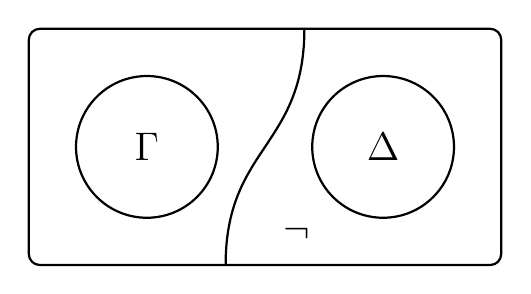
\begin{tikzpicture}[node distance=2cm, auto, thick]
    \draw [rounded corners] (0,0) -- (6,0) -- (6,3) -- (0,3) --  cycle;
    \draw (1.5,1.5) circle (0.9cm);
    \draw (4.5,1.5) circle (0.9cm);
    \path node at (1.5,1.5) {\Large $\Gamma$};
    \path node at (4.5,1.5) {\Large $\Delta$};
    \path node at (0.4,2.6) {\Large $\formula{C}$};
    \path node at (3.4,0.4) {\Large $\lnot \formula{C}$};
    \draw (2.5,0) .. controls (2.5,1.5) and (3.5,1.5) .. (3.5,3);
  \end{tikzpicture}
  \caption{$\chi$, $\Gamma$ અને~$\Delta$ને પૃથક કરે છે}
  \ollabel{fig:sep}
\end{figure}


\begin{lem}\ollabel{lem:sep1}
ધારો કે $\Lang{L}_0$ એ એવી ભાષા છે જેમાં $\Gamma$ અને~$\Delta$
\emph{બંને}માં આવતા દરેક અચળ, વિધેય અને વિધેય
($\doteq$ સિવાયના) છે, અને $n\ge 0$ માટે અનંત નવા અચળો
$\Obj c_n$ ઉમેરીને $\Lang{L}'_0$ મેળવાય છે. તો જો $\Gamma$ અને
$\Delta$, $\Lang{L}_0$માં અપૃથક્કરણીય હોય, તો તેઓ $\Lang{L}'_0$માં
પણ અપૃથક્કરણીય છે.
\end{lem}

\begin{proof}
આપણે પરોક્ષ રીતે આગળ વધીએ: વિરોધાભાસ માટે ધારો કે $\Gamma$ અને
$\Delta$, $\Lang{L}'_0$માં પૃથક્કરણીય છે. તો કોઈ $\chi\in\Lang{L}_0$
માટે $\Gamma \Entails \Subst{\chi}{c}{x}$ અને $\Delta \Entails \lnot
\Subst{\chi}{c}{x}$ (અહીં $c$ નવો અચળ છે---$\chi$માં આવા એકથી
વધુ નવા અચળ હોય તે કિસ્સો સમાન છે). સઘનતાથી, $\Gamma$નો
કોઈ \emph{સાન્ત} ઉપગણ~$\Gamma_0$ અને $\Delta$નો કોઈ \emph{સાન્ત}
ઉપગણ~$\Delta_0$ એવા છે કે $\Gamma_0 \Entails \Subst{\chi}{c}{x}$ અને
$\Delta_0 \Entails \lnot \Subst{\chi}{c}{x}$. $\Gamma_0$નાં બધાં
સૂત્રોના સંયોજનને~$\gamma$ અને $\Delta_0$નાં બધાં સૂત્રોના
સંયોજનને~$\delta$ કહો. તો
\begin{align*}
  \gamma & \Entails \Subst{\chi}{c}{x}, & \delta  \Entails \lnot \Subst{\chi}{c}{x}.
\end{align*}
પહેલામાંથી સર્વત્રીકરણ વડે $\gamma \Entails \lforall[x][\chi]$ મળે છે;
બીજામાંથી પ્રતિપક્ષન વડે $\Subst{\chi}{c}{x} \Entails \lnot \delta$, અને
તેથી $\lforall[x][\chi] \Entails \lnot \delta$ પણ મળે છે. ફરી પ્રતિપક્ષનથી
$\delta \Entails \lnot \lforall[x][\chi]$. એકદિશવર્ધિતાથી,
\begin{align*}
  \Gamma &\Entails \lforall[x][\chi], &
  \Delta & \Entails \lnot \lforall[x][\chi],
\end{align*}
અને તેથી $\lforall[x][\chi]$, $\Gamma$ અને~$\Delta$ને $\Lang{L}_0$માં
પૃથક કરે છે.
\sourcecorrection{OLINT-001}{સ્થિર અંગ્રેજી મૂળની
  \texttt{separation.tex}, પંક્તિ~75માં પૂર્વધારણા~$\delta$ના સ્થાને
  અગાઉ ક્યાંય વ્યાખ્યાયિત ન થયેલું~$\delta$ આવે છે. પ્રતિપક્ષનથી
  મેળવવાના નિષ્કર્ષમાં અહીં $\lnot \delta$ પુનઃસ્થાપિત કર્યું છે.}
\end{proof}

\begin{lem}\ollabel{lem:sep2}
ધારો કે $\Gamma \cup \{ \lexists[x][\sigma] \}$ અને~$\Delta$
અપૃથક્કરણીય છે, અને $c$ એવો નવો અચળ છે જે $\Gamma$,
$\Delta$ કે~$\sigma$માં આવતો નથી. તો $\Gamma \cup \{ \lexists[x][\sigma],
\Subst{\sigma}{c}{x} \}$ અને~$\Delta$ પણ અપૃથક્કરણીય છે.
\end{lem}

\begin{proof}
વિરોધાભાસ માટે ધારો કે $\chi$, $\Gamma \cup \{ \lexists[x][\sigma],
\Subst{\sigma}{c}{x}\}$ અને~$\Delta$ને પૃથક કરે છે, જ્યારે $\Gamma \cup
\{\lexists[x][\sigma] \}$ અને~$\Delta$ અપૃથક્કરણીય છે. આપણે બે કિસ્સા
પાડીએ છીએ:
\sourcecorrection{OLINT-002}{સ્થિર અંગ્રેજી મૂળની
  \texttt{separation.tex}, પંક્તિ~95માં $\lexists$ના સૂત્ર-દલીલખંડને
  જરૂરી ચોરસ કૌંસને બદલે વાંકિયા કૌંસમાં મૂક્યો છે; તેથી તે
  ક્વાન્ટિફાયરના વ્યાપ તરીકે લેવાતો નથી. અહીં
  \texttt{\string\lexists[x][\sigma]} પુનઃસ્થાપિત કર્યું છે.}
\begin{enumerate}
\item $c$, $\chi$માં આવતો નથી: આ કિસ્સામાં $\Gamma \cup
  \{\lexists[x][\sigma], \lnot\chi \}$ સંતોષ્ય છે (નહિતર $\chi$, $\Gamma
  \cup \{\lexists[x][\sigma] \}$ અને~$\Delta$ને પૃથક કરે). તેમાં
  $\Subst{\sigma}{c}{x}$ ઉમેર્યા પછી પણ તે સંતોષ્ય રહે છે, તેથી અંતે
  $\chi$, $\Gamma \cup \{ \lexists[x][\sigma], \Subst{\sigma}{c}{x} \}$ અને
  $\Delta$ને પૃથક કરતું નથી.
\item $c$, $\chi$માં આવે છે, જેથી $\chi$નું સ્વરૂપ
  $\Subst{\chi}{c}{x}$ છે. ત્યારે
  \[
  \Gamma \cup \{ \lexists[x][\sigma], \Subst{\sigma}{c}{x}\} \Entails \Subst{\chi}{c}{x},
  \]
  અને તેથી નિગમન પ્રમેય તથા સર્વત્રીકરણ વડે
  $\Gamma, \lexists[x][\sigma] \Entails \lforall[x][(\sigma \lif \chi)]$,
  અને છેવટે $\Gamma \cup \{ \lexists[x][\sigma] \} \Entails
  \lexists[x][\chi]$. બીજી તરફ, $\Delta \Entails \lnot
  \Subst{\chi}{c}{x}$ અને તેથી સર્વત્રીકરણ વડે $\Delta \Entails \lnot
  \lexists[x][\chi]$. એટલે $\Gamma \cup \{\lexists[x][\sigma] \}$ અને
  $\Delta$ પૃથક્કરણીય છે, જે વિરોધાભાસ છે.
\end{enumerate}
\end{proof}




\olfileid{mod}{int}{prf}

\subsection{ક્રેગનું અંતર્વેશન પ્રમેય}

\begin{thm}[ક્રેગનું અંતર્વેશન પ્રમેય]
\ollabel{thm:interpol}
જો $\Entails \varphi \lif \psi$, તો એવું વાક્ય~$\chi$ છે કે
$\Entails \varphi \lif \chi$ અને $\Entails \chi \lif \psi$, અને $\chi$માં આવતો
દરેક અચળ, વિધેય અને વિધેય ($\eq$ સિવાયનો)
$\varphi$ અને~$\psi$ બંનેમાં આવે છે. વાક્ય~$\chi$ને $\varphi$ અને~$\psi$નો
\emph{અંતર્વેશક} કહે છે.
\end{thm}

\begin{proof}
ધારો કે $\Lang{L}_1$, $\varphi$ની ભાષા છે અને $\Lang{L}_2$, $\psi$ની ભાષા
છે. $\Lang{L}_0 = \Lang{L}_1 \cap \Lang{L}_2$ રાખો. દરેક $i \in
\{0, 1, 2 \}$ માટે, $\Lang{L}_i$માં અનંત નવા અચળો
$\Obj c_0, \Obj c_1, \Obj c_2, \dots$ ઉમેરીને $\Lang{L}'_i$ મેળવો.

જો $\varphi$ અસંતોષ્ય હોય, તો $\lexists[x][\eq/[x][x]]$ અંતર્વેશક છે.
જો $\lnot \psi$ અસંતોષ્ય હોય (અને તેથી $\psi$ પ્રામાણ્ય હોય), તો
$\lexists[x][\eq[x][x]]$ અંતર્વેશક છે. તેથી આપણે $\varphi$ અને
$\lnot \psi$ બંને સંતોષ્ય છે એમ પણ ધારી શકીએ છીએ.

અંતર્વેશન પ્રમેયનું પ્રતિપક્ષી સ્વરૂપ સાબિત કરવા માટે ધારો કે $\varphi$
અને~$\psi$ માટે કોઈ અંતર્વેશક નથી. બીજા શબ્દોમાં, ધારો કે $\{\varphi\}$ અને
$\{\lnot \psi\}$, $\Lang{L}_0$માં અપૃથક્કરણીય છે.

આપણો ઉદ્દેશ જોડ $(\{ \varphi \}, \{\lnot\psi\})$ને કોઈ મહત્તમ
અપૃથક્કરણીય જોડ $(\Gamma^*, \Delta^*)$ સુધી વિસ્તારવાનો છે.
$\varphi_0$, $\varphi_1$, $\varphi_2$,~\dots એ $\Lang{L}'_1$નાં વાક્યોની
ગણના અને $\psi_0$, $\psi_1$, $\psi_2$,~\dots એ $\Lang{L}'_2$નાં
વાક્યોની ગણના હોય. નીચે પ્રમાણે $n\ge0$ માટે વાક્યોના
ગણોની બે વધતી શ્રેણીઓ $(\Gamma_n,\Delta_n)$ વ્યાખ્યાયિત કરીએ. $\Gamma_0
= \{\varphi\}$ અને $\Delta_0=\{\lnot \psi\}$ રાખો. $(\Gamma_n,\Delta_n)$
પહેલેથી વ્યાખ્યાયિત છે એમ ધારીને, $\Gamma_{n+1}$ અને
$\Delta_{n+1}$ને આ પ્રમાણે વ્યાખ્યાયિત કરો:
\sourcecorrection{OLINT-003}{સ્થિર અંગ્રેજી મૂળની
  \texttt{interpolation-proof.tex}, પંક્તિઓ~41--43માં $\varphi_n$ અને
  $\psi_n$ને અનુક્રમે $\Lang{L}_1$ અને $\Lang{L}_2$નાં વાક્યોની ગણના
  કહેવાય છે. પરંતુ પછીની પંક્તિઓ~107--108માં રચાયેલા ગણો
  $\Lang{L}'_1$ અને $\Lang{L}'_2$માં પૂર્ણ સુસંગત હોવાનો દાવો થાય છે,
  જેના માટે નવા અચળો ધરાવતાં વાક્યોની પણ ગણના જરૂરી છે. અહીં બંને
  વિસ્તૃત ભાષાઓ પર ગણના પુનઃસ્થાપિત કરી છે.}
\begin{enumerate}
\item જો $\Gamma_n \cup \{\varphi_n \}$ અને~$\Delta_n$, $\Lang{L}'_0$માં
  અપૃથક્કરણીય હોય, તો $\varphi_n$ને $\Gamma_{n+1}$માં મૂકો. વધુમાં, જો
  $\varphi_n$ કોઈ અસ્તિત્વવાચક સૂત્ર~$\lexists[x][\sigma]$ હોય, તો
  $\Gamma_n$, $\Delta_n$, $\varphi_n$ કે~$\psi_n$માં ન આવતો નવો
  અચળ~$c$ પસંદ કરીને $\Subst{\sigma}{c}{x}$ને
  $\Gamma_{n+1}$માં મૂકો.
\item જો $\Gamma_{n+1}$ અને $\Delta_n \cup \{\psi_n \}$,
  $\Lang{L}'_0$માં અપૃથક્કરણીય હોય, તો $\psi_n$ને $\Delta_{n+1}$માં
  મૂકો. વધુમાં, જો $\psi_n$ કોઈ અસ્તિત્વવાચક
  સૂત્ર~$\lexists[x][\sigma]$ હોય, તો $\Gamma_{n+1}$, $\Delta_n$,
  $\varphi_n$ કે~$\psi_n$માં ન આવતો નવો અચળ~$c$ પસંદ કરીને
  $\Subst{\sigma}{c}{x}$ને $\Delta_{n+1}$માં મૂકો.
\end{enumerate}
છેવટે, આ પ્રમાણે વ્યાખ્યા કરો:
\begin{align*}
  \Gamma^* & = \bigcup_{n\ge 0} \Gamma_n, &
  \Delta^* & = \bigcup_{n\ge 0} \Delta_n.
\end{align*}
હવે $n$ પરના સમકાલીન આગમનથી આપણે નીચેના દાવા સાબિત કરી શકીએ છીએ:
\begin{enumerate}
\item\ollabel{part-a} $\Gamma_n$ અને~$\Delta_n$, $\Lang{L}'_0$માં
  અપૃથક્કરણીય છે;
\item\ollabel{part-b} $\Gamma_{n+1}$ અને~$\Delta_n$,
  $\Lang{L}'_0$માં અપૃથક્કરણીય છે.
\end{enumerate}
\olref{part-a}નો આધાર \olref[sep]{lem:sep1} આપે છે. ભાગ
\olref{part-b} માટે આપણે ત્રણ કિસ્સા પાડવા પડે છે:
\begin{enumerate}
\item જો $\Gamma_0 \cup \{\varphi_0 \}$ અને~$\Delta_0$ પૃથક્કરણીય હોય,
  તો $\Gamma_1=\Gamma_0$ અને \olref{part-b}, \olref{part-a} જ છે;
\item જો $\Gamma_1 = \Gamma_0 \cup\{\varphi_0\}$, તો રચના મુજબ
  $\Gamma_1$ અને~$\Delta_0$ અપૃથક્કરણીય છે.
\item હવે માત્ર $\varphi_0$ અસ્તિત્વવાચક હોય તે કિસ્સો બાકી રહે છે, જેમાં
  $\Gamma_1 = \Gamma_0 \cup \{ \lexists[x][\sigma], \Subst{\sigma}{c}{x}
  \}$. રચના મુજબ $\Gamma_0 \cup \{ \lexists[x][\sigma]\}$ અને
  $\Delta_0$ અપૃથક્કરણીય છે, તેથી \olref[sep]{lem:sep2} મુજબ
  $\Gamma_0 \cup \{ \lexists[x][\sigma], \Subst{\sigma}{c}{x} \}$ અને
  $\Delta_0$ પણ અપૃથક્કરણીય છે.
\end{enumerate}
આથી ઉપરના \olref{part-a} અને \olref{part-b} માટે આગમનનો આધાર પૂરો
થાય છે. હવે આગમન-પગલું લઈએ. \olref{part-a} માટે, જો $\psi_n$ને
$\Delta_{n+1}$માં મૂકવામાં આવે, તો રચના મુજબ $\Gamma_{n+1}$ અને
$\Delta_n\cup\{\psi_n\}$ અપૃથક્કરણીય છે; અને જો $\psi_n$ અસ્તિત્વવાચક
હોય, તો સાક્ષી ઉમેર્યા પછીનો $\Delta_{n+1}$ પણ
\olref[sep]{lem:sep2} મુજબ અપૃથક્કરણીય રહે છે. જો
$\Delta_{n+1}=\Delta_n$ (કારણ કે $\Gamma_{n+1}$ અને
$\Delta_n\cup\{\psi_n\}$ પૃથક્કરણીય છે), તો \olref{part-b} માટેની
આગમન-પરિકલ્પના વાપરીએ. \olref{part-b}ના આગમન-પગલા માટે, જો
$\varphi_{n+1}$ને $\Gamma_{n+2}$માં મૂકવામાં આવે, તો રચના મુજબ
$\Gamma_{n+1}\cup\{\varphi_{n+1}\}$ અને~$\Delta_{n+1}$ અપૃથક્કરણીય છે;
અને જો $\varphi_{n+1}$ અસ્તિત્વવાચક હોય, તો સાક્ષી ઉમેર્યા પછીનો
$\Gamma_{n+2}$ પણ \olref[sep]{lem:sep2} મુજબ અપૃથક્કરણીય રહે છે. જો
$\Gamma_{n+2}=\Gamma_{n+1}$, તો હમણાં જ સાબિત કરેલો
\olref{part-a}નો આગમન-કિસ્સો વાપરીએ. આથી \olref{part-a} અને
\olref{part-b} પરનું આગમન પૂરું થાય છે.
\sourcecorrection{OLINT-004}{સ્થિર અંગ્રેજી મૂળની
  \texttt{interpolation-proof.tex}, પંક્તિઓ~88--96માં અસ્તિત્વવાચક
  $\psi_n$ કે $\varphi_{n+1}$ સ્વીકારાય ત્યારે સાક્ષી-સૂત્ર પણ ઉમેરવાની
  અગાઉની સૂચના હોવા છતાં અનુક્રમે
  $\Delta_{n+1}=\Delta_n\cup\{\psi_n\}$ અને
  $\Gamma_{n+2}=\Gamma_{n+1}\cup\{\varphi_{n+1}\}$ લખાયું છે. અહીં
  સ્વીકારેલો વિધાન અને પછી ઉમેરાતો સાક્ષી અલગ કરીને, લેમા
  \olref[sep]{lem:sep2}નો ઉપયોગ બંને પૂર્ણ ગણો પર સ્પષ્ટ કર્યો છે.}

આમાંથી ફલિત થાય છે કે $\Gamma^*$ અને~$\Delta^*$ અપૃથક્કરણીય છે;
નહિતર સઘનતાથી એવું $n\ge0$ અને એવું $\Lang{L}'_0$-વિધાન મળે જે
$\Gamma_n$ અને~$\Delta_n$ને પૃથક કરે, જે \olref{part-a}ની વિરુદ્ધ
છે. ખાસ કરીને, $\Gamma^*$ અને~$\Delta^*$ સુસંગત છે: કારણ કે પહેલો
અથવા બીજો અસુસંગત હોય, તો અનુક્રમે $\lexists[x][\eq/[x][x]]$ અથવા
$\lforall[x][\eq[x][x]]$ તેમને પૃથક કરે.
\sourcecorrection{OLINT-005}{સ્થિર અંગ્રેજી મૂળની
  \texttt{interpolation-proof.tex}, પંક્તિઓ~100--102માં કોઈ
  $n\ge0$ પોતે $\Gamma_n$ અને $\Delta_n$ને પૃથક કરે છે તેમ લખાયું
  છે. પૃથક્કર્તા વિધાન હોય છે; સઘનતા માત્ર એવું એક જ~$n$ આપે છે જેમાં
  તેના માટે જરૂરી બંને સાન્ત ઉપગણો આવી જાય. અહીં એ વિધાન અને~$n$ની
  જુદી ભૂમિકાઓ સ્પષ્ટ કરી છે.}

હવે આપણે બતાવીએ કે $\Gamma^*$, $\Lang{L}'_1$માં પૂર્ણ સુસંગત છે અને
એ જ રીતે $\Delta^*$, $\Lang{L}'_2$માં પૂર્ણ સુસંગત છે. પહેલા માટે,
ધારો કે કોઈ $n\ge0$ માટે $\varphi_n\notin\Gamma^*$ અને $\lnot \varphi_n
\notin\Gamma^*$. જો $\varphi_n\notin\Gamma^*$, તો $\Gamma_n\cup\{\varphi_n\}$
$\Delta_n$થી પૃથક્કરણીય છે, તેથી એવું $\chi\in\Lang{L}'_0$ છે કે આ
બંને વાતો સાચી છે:
\begin{align*}
  \Gamma^* & \Entails \varphi_n \lif \chi, &
  \Delta^* & \Entails \lnot \chi.
\end{align*}
એ જ રીતે, જો $\lnot \varphi_n\notin\Gamma^*$, તો એવું $\chi'\in
\Lang{L}'_0$ છે કે આ બંને વાતો સાચી છે:
\begin{align*}
  \Gamma^* & \Entails \lnot \varphi_n \lif \chi', &
  \Delta^* & \Entails \lnot \chi'.
\end{align*}
વિધાનાત્મક તર્કશાસ્ત્રથી $\Gamma^*\Entails \chi\lor \chi'$ અને
$\Delta^*\Entails\lnot(\chi\lor \chi')$, તેથી $\chi\lor \chi'$,
$\Gamma^*$ અને~$\Delta^*$ને પૃથક કરે છે. સમાન દલીલથી $\Delta^*$ પૂર્ણ
છે.

છેવટે, આપણે બતાવીએ કે $\Gamma^*\cap\Delta^*$, $\Lang{L}'_0$માં પૂર્ણ
સુસંગત છે. તે સુસંગત ગણોનો છેદ હોવાથી દેખીતી રીતે સુસંગત છે. પૂર્ણતા
બતાવવા $\sigma\in\Lang{L}'_0$ લો. હવે $\Gamma^*$, $\Lang{L'_1}
\supseteq\Lang{L'_0}$માં પૂર્ણ છે અને એ જ રીતે $\Delta^*$,
$\Lang{L'_2}\supseteq\Lang{L'_0}$માં પૂર્ણ છે. તેથી કાં તો
$\sigma\in\Gamma^*$ અથવા $\lnot \sigma\in\Gamma^*$, અને કાં તો
$\sigma\in\Delta^*$ અથવા $\lnot \sigma\in\Delta^*$. જો $\sigma\in\Gamma^*$ અને
$\lnot \sigma\in\Delta^*$, તો $\sigma$, $\Gamma^*$ અને~$\Delta^*$ને પૃથક
કરે; અને જો $\lnot \sigma\in\Gamma^*$ અને $\sigma\in\Delta^*$, તો
$\Gamma^*$ અને~$\Delta^*$ને $\lnot \sigma$ પૃથક કરે. આથી, કાં તો
$\sigma\in\Gamma^*\cap\Delta^*$
અથવા $\lnot \sigma\in\Gamma^*\cap\Delta^*$, અને
$\Gamma^*\cap\Delta^*$ પૂર્ણ છે.

$\Gamma^*$ પૂર્ણ સુસંગત હોવાથી તેને એવો નિદર્શ $\Struct{M}'_1$ મળે
છે જેનું વ્યાપકક્ષેત્ર~$\Domain{M'_1}$, અચળોનાં અર્થઘટનો
$\Assign{c}{M'_1}$ એવા અને માત્ર એવા ઘટકોનું બનેલું છે---પૂર્ણતા
પ્રમેયની સાબિતીની જેમ (\olref[fol][com][cth]{thm:completeness}). એ જ
રીતે, $\Delta^*$ને એવો નિદર્શ~$\Struct{M}'_2$ મળે છે જેનું
વ્યાપકક્ષેત્ર~$\Domain{M'_2}$, અચળોનાં અર્થઘટનો
$\Assign{c}{M'_2}$થી બનેલું છે.

$\Struct{M'_1}$માંથી $\Lang{L'_1}\setminus\Lang{L'_0}$માંના
અચળો, વિધેયો અને વિધેયોનાં અર્થઘટનો કાઢીને
$\Struct{M_1}$ મેળવો, અને $\Struct{M_2}$ પણ એ જ રીતે મેળવો. ત્યારે
$h(\Assign{c}{M'_1})=\Assign{c}{M'_2}$થી વ્યાખ્યાયિત કરેલો નકશો
$h\colon M_1\to M_2$, $\Lang{L}'_0$માં એકરૂપતા છે, કારણ કે બતાવ્યા
પ્રમાણે $\Gamma^*\cap\Delta^*$, $\Lang{L}'_0$માં પૂર્ણ સુસંગત છે.
આનું કારણ એ છે કે કોઈ પણ $\Lang{L}'_0$-વાક્ય કાં તો $\Gamma^*$
અને~$\Delta^*$ બંનેમાં આવે છે અથવા એકેયમાં આવતું નથી: તેથી
$\Assign{c}{M'_1}\in\Assign{P}{M'_1}$ જો અને માત્ર જો
$\Atom{P}{c}\in\Gamma^*$, જો અને માત્ર જો $\Atom{P}{c}\in\Delta^*$,
જો અને માત્ર જો $\Assign{c}{M'_2}\in\Assign{P}{M'_2}$. એકરૂપતાની
બીજી શરતો પણ એ જ રીતે સ્થાપિત કરી શકાય છે.

હવે ભાષા~$\Lang{L_1}\cup\Lang{L_2}$ માટેનો નિદર્શ
$\Struct{M}$ આ પ્રમાણે વ્યાખ્યાયિત કરીએ:
\begin{enumerate}
\item વ્યાપકક્ષેત્ર~$\Domain{M}$ એ $\Domain{M_2}$ જ છે, એટલે બધા
  ઘટકો~$\Assign{c}{M'_2}$નો ગણ;
\item જો કોઈ વિધેય~$P$, $\Lang{L_2}\setminus\Lang{L_1}$માં
  હોય, તો $\Assign{P}{M}=\Assign{P}{M'_2}$;
\item જો કોઈ વિધેય-સંકેત~$P$, $\Lang{L}_1\setminus\Lang{L}_2$માં હોય, તો
  $\Assign{P}{M}=h(\Assign{P}{M'_1})$, એટલે
  $\tuple{\Assign{c_1}{M'_2},\dots,\Assign{c_n}{M'_2}}\in
  \Assign{P}{M}$ જો અને માત્ર જો
  $\tuple{\Assign{c_1}{M'_1},\dots,\Assign{c_n}{M'_1}}\in
  \Assign{P}{M'_1}$.
\item જો કોઈ વિધેય~$P$, $\Lang{L}_0$માં હોય, તો
  $\Assign{P}{M}=\Assign{P}{M'_2}=h(\Assign{P}{M'_1})$.
\item વિધેયોને, જેમાં અચળો પણ સામેલ છે,
  $\Lang{L}_1\cup\Lang{L}_2$ પર એ જ રીતે સંભાળો.
\end{enumerate}
\sourcecorrection{OLINT-006}{સ્થિર અંગ્રેજી મૂળની
  \texttt{interpolation-proof.tex}, પંક્તિ~173માં
  $P\in\Lang{L}_1\setminus\Lang{L}_2$ હોવા છતાં તેના અર્થઘટનને
  $\Struct{M'_2}$માંથી લઈ $h$ લગાડવામાં આવ્યું છે. $\Struct{M'_2}$
  પાસે $P$નું અર્થઘટન હોવું જરૂરી નથી અને $h$નું ક્ષેત્ર પણ
  $M_1$ છે. તરત પછી આપેલી ``એટલે'' શરત મુજબ અહીં
  $h(\Assign{P}{M'_1})$ પુનઃસ્થાપિત કર્યું છે.}

છેવટે, સૂત્રો પરના આગમનથી બતાવી શકાય છે કે $\Lang{L}_1$નાં
બધાં સૂત્રો માટે $\Struct{M'_1}$ના $\Lang{L}_1$-ન્યૂનરૂપમાં
સંતોષ, $h$ મારફતે $\Struct{M}$ના $\Lang{L}_1$-ન્યૂનરૂપમાં સંતોષને
બરાબર અનુરૂપ છે, અને $\Lang{L}_2$નાં બધાં સૂત્રો માટે
$\Struct{M}$ તથા $\Struct{M'_2}$નાં $\Lang{L}_2$-ન્યૂનરૂપોમાં સંતોષ
સંમત થાય છે. ખાસ કરીને,
$\Struct{M'_1}\Entails\Gamma^*$ તથા $\varphi\in\Gamma^*$, અને
$\Struct{M'_2}\Entails\Delta^*$ તથા $\lnot \psi\in\Delta^*$ હોવાથી
$\Struct{M}\Entails \varphi$ અને $\Struct{M}\Entails\lnot \psi$. તેથી
$\not\Entails \varphi\lif \psi$. આથી ક્રેગના અંતર્વેશન પ્રમેયની સાબિતી
પૂરી થાય છે.
\sourcecorrection{OLINT-007}{સ્થિર અંગ્રેજી મૂળની
  \texttt{interpolation-proof.tex}, પંક્તિઓ~183--187માં
  $\Struct{M}$ને માત્ર $\Lang{L}_1\cup\Lang{L}_2$ માટે વ્યાખ્યાયિત
  કર્યા પછી તે નવા અચળો ધરાવતી વિસ્તૃત ભાષાઓ $\Lang{L}'_1$ અને
  $\Lang{L}'_2$નાં બધાં સૂત્રો પર સંમત થાય છે અને
  $\Gamma^*\cup\Delta^*$ને સંતોષે છે એવો અપરિભાષિત દાવો થાય છે.
  અહીં જરૂરી અને પર્યાપ્ત ન્યૂનરૂપ-દાવો મૂક્યો છે: $h$ પહેલા નિદર્શના
  $\Lang{L}_1$-ભાગને પરિવહિત કરે છે અને બીજાનો
  $\Lang{L}_2$-ભાગ યથાવત્ રહે છે; તેથી મૂળ વાક્યો $\varphi$ અને
  $\lnot \psi$ સાચાં રહે છે.}
\end{proof}




\olfileid{mod}{int}{def}

\subsection{વ્યાખ્યેયતા પ્રમેય}

અંતર્વેશન પ્રમેયનો એક મહત્વનો ઉપયોગ બેથનું વ્યાખ્યેયતા પ્રમેય છે.
$n$-સ્થાની સંબંધ~$R$ને વ્યાખ્યાયિત કરવા માટે આપણે $R$ ન આવતો હોય
અને $n$ મુક્ત ચલો ધરાવતો કોઈ સૂત્ર~$\chi$ આપી શકીએ
છીએ. આ $\chi$ દ્વારા $R$ની \emph{સ્પષ્ટ} વ્યાખ્યા થાય. પછી આપણે એમ
પણ કહી શકીએ કે $n$-સ્થાની વિધેય~$P$ ધરાવતી કોઈ ભાષામાં
સિદ્ધાંત~$\Sigma(P)$, $P$ને સ્પષ્ટ રીતે વ્યાખ્યાયિત કરે છે જો તેમાં
ઔપચારિક કરેલી સ્પષ્ટ વ્યાખ્યા હોય (અથવા ઓછામાં ઓછું તેમાંથી ફલિત થતી
હોય), એટલે કે,
\[
\Sigma(P) \Entails \lforall[x_1][\dots
  \lforall[x_n][(\Atom{P}{x_1,\dots, x_n} \liff \chi(x_1, \dots,
    x_n))]].
\]
પરંતુ સંબંધને વ્યાખ્યાયિત કરવાનો---તેને સંપૂર્ણપણે નિશ્ચિત કરવાના
અર્થમાં---સ્પષ્ટ વ્યાખ્યા માત્ર એક માર્ગ છે. સિદ્ધાંત એવો પણ હોઈ શકે
કે કોઈ પણ નિદર્શમાં ભાષાના બાકીના ભાગના અર્થઘટનથી $P$નું
અર્થઘટન નિશ્ચિત થાય. વ્યાખ્યેયતા પ્રમેય કહે છે કે જ્યારે પણ સિદ્ધાંત
$P$નું અર્થઘટન આ રીતે નિશ્ચિત કરે---જ્યારે તે $P$ને \emph{ગૂઢ રીતે
વ્યાખ્યાયિત કરે}---ત્યારે તે તેને સ્પષ્ટ રીતે પણ વ્યાખ્યાયિત કરે છે.

\begin{defn}
ધારો કે $\Lang{L}$ એવી ભાષા છે જેમાં વિધેય~$P$ નથી.
$\Lang{L}\cup\{P\}$નાં વાક્યોનો ગણ~$\Sigma(P)$, $P$ને ત્યારે
અને માત્ર ત્યારે \emph{સ્પષ્ટ રીતે વ્યાખ્યાયિત કરે છે} જ્યારે
$\Lang{L}$નું એવું સૂત્ર~$\chi(x_1,\dots,x_n)$ છે કે
\[
\Sigma(P) \Entails \lforall[x_1][\dots
  \lforall[x_n][(\Atom{P}{x_1,\dots, x_n} \liff \chi(x_1, \dots,
    x_n))]].
\]
\end{defn}

\begin{defn}
ધારો કે $\Lang{L}$ એવી ભાષા છે જેમાં વિધેયો $P$
અને~$P'$ નથી. $\Lang{L}\cup\{P\}$નાં વાક્યોનો ગણ~$\Sigma(P)$,
$P$ને ત્યારે અને માત્ર ત્યારે \emph{ગૂઢ રીતે વ્યાખ્યાયિત કરે છે}
જ્યારે
\[
\Sigma(P) \cup \Sigma(P') \Entails \lforall[x_1][\dots
  \lforall[x_n][(\Atom{P}{x_1,\dots, x_n} \liff \Atom{P'}{x_1,\dots,
      x_n})]],
\]
જ્યાં $\Sigma(P')$ એ $\Sigma(P)$માં $P$ને સર્વત્ર $P'$થી બદલીને
મળતું પરિણામ છે.
\end{defn}

બીજા શબ્દોમાં, કોઈ પણ નિદર્શ~$\Struct{M}$ અને $R,R'\subseteq
\Domain{M}^n$ માટે, જો $\Expan{M}{R}\Entails\Sigma(P)$ અને
$\Expan{M}{R'}\Entails\Sigma(P')$ બંને, તો $R=R'$; અહીં
$\Expan{M}{R}$ એ $\Lang{L}$ના $\Lang{L}\cup\{P\}$ સુધીના વિસ્તાર
માટેની એવી સંરચના~$\Struct{M'}$ છે કે $\Assign{P}{M'}=R$, અને
$\Expan{M}{R'}$ માટે પણ એ જ રીતે.

\begin{thm}[બેથનું વ્યાખ્યેયતા પ્રમેય]
$\Lang{L}\cup\{P\}$નાં વાક્યોનો ગણ~$\Sigma(P)$, $P$ને ગૂઢ
રીતે વ્યાખ્યાયિત કરે છે જો અને માત્ર જો $\Sigma(P)$, $P$ને સ્પષ્ટ
રીતે વ્યાખ્યાયિત કરે છે.
\end{thm}
\sourcecorrection{OLINT-008}{સ્થિર અંગ્રેજી મૂળની
  \texttt{definability.tex}, પંક્તિઓ~66--68માં પ્રમેય $\Sigma(P)$ને
  સૂત્રોનો ગણ કહે છે, જ્યારે તરત અગાઉની બંને વ્યાખ્યાઓ તેને
  વાક્યોનો ગણ કહે છે અને નીચેની સાબિતી પણ સાન્ત ઉપગણનાં
  વાક્યોના સંયોજન પર ચાલે છે. અહીં વ્યાખ્યાઓ અને સાબિતી મુજબ
  વાક્યો પુનઃસ્થાપિત કર્યાં છે.}
\sourcecorrection{OLINT-009}{એ જ મૂળની પંક્તિ~67માં દ્વિમુખી શરતના
  ``if and only if''માંથી છેલ્લું ``if'' છૂટી ગયું છે. અહીં સંપૂર્ણ
  દ્વિમુખી શરત પુનઃસ્થાપિત કરી છે.}

\begin{proof}
જો $\Sigma(P)$, $P$ને સ્પષ્ટ રીતે વ્યાખ્યાયિત કરે, તો આ બંને સાચાં
છે:
\begin{align*}
  \Sigma(P) & \Entails & \lforall[x_1][\dots \lforall[x_n]
    [(\Atom{P}{x_1,\dots, x_n} \liff \chi(x_1,\dots,x_n))]]\\
  \Sigma(P') & \Entails & \lforall[x_1][\dots \lforall[x_n]
    [(\Atom{P'}{x_1,\dots, x_n} \liff \chi(x_1,\dots,x_n))]]
\end{align*}
અને નિષ્કર્ષ ફલિત થાય છે. વ્યસ્ત દિશા માટે ધારો કે $\Sigma(P)$,
$P$ને ગૂઢ રીતે વ્યાખ્યાયિત કરે છે. પહેલા $\Lang{L}$માં અચળો
$c_1$,~\dots,~$c_n$ ઉમેરીએ. ત્યારે
\[
\Sigma(P) \cup \Sigma(P') \Entails
\Atom{P}{c_1, \dots, c_n} \to \Atom{P'}{c_1, \dots, c_n}.
\]
સઘનતાથી એવા સાન્ત ગણો $\Delta_0\subseteq\Sigma(P)$ અને
$\Delta_1\subseteq\Sigma(P')$ છે કે
\[
\Delta_0 \cup \Delta_1 \Entails
\Atom{P}{c_1, \dots, c_n} \to \Atom{P'}{c_1, \dots, c_n}.
\]
એવા બધા વાક્યો~$\varphi(P)$નું સંયોજન~$\theta(P)$ કહો કે કાં તો
$\varphi(P)\in\Delta_0$ અથવા $\varphi(P')\in\Delta_1$, અને એવા બધા
વાક્યો~$\varphi(P')$નું સંયોજન~$\theta(P')$ કહો કે કાં તો
$\varphi(P)\in\Delta_0$ અથવા $\varphi(P')\in\Delta_1$. ત્યારે
$\theta(P)\land \theta(P')\Entails\Atom{P}{c_1,\dots,c_n}\to
\Atom{P'}{c_1,\dots,c_n}$. આને એવી રીતે ફરી ગોઠવી શકાય કે દરેક
વિધેય, $\Entails$ની એક બાજુ જ આવે:
\sourcecorrection{OLINT-010}{સ્થિર અંગ્રેજી મૂળની
  \texttt{definability.tex}, પંક્તિ~96માં જમણી બાજુનું પરમાણુક સૂત્ર
  આસપાસનાં બધાં દાખલાથી જુદું $P'c_1\dots c_n$ લખાયું છે. અહીં એ જ
  $n$-સ્થાની પરમાણુક સૂત્ર માટેનું આવૃત્તિ-સુસંગત
  \texttt{\string\Atom\{P'\}\{c\_1,\string\dots,c\_n\}} સ્વરૂપ વાપર્યું
  છે.}
\[
\theta(P) \land \Atom{P}{c_1, \dots, c_n} \Entails
\theta(P') \to \Atom{P'}{c_1, \dots, c_n}.
\]
ક્રેગના અંતર્વેશન પ્રમેય મુજબ $P$ કે~$P'$ ન ધરાવતું એવું
વાક્ય~$\chi(c_1,\dots,c_n)$ છે કે
\begin{align*}
  \theta(P) \land \Atom{P}{c_1, \dots, c_n} & \Entails \chi(c_1,\dots, c_n); \\
  \chi(c_1,\dots, c_n) & \Entails \theta(P') \to \Atom{P'}{c_1, \dots, c_n}.
\end{align*}
આ બે ફલિતતાઓમાંથી પહેલામાંથી મળે છે: $\theta(P)\Entails
\Atom{P}{c_1,\dots,c_n}\lif \chi(c_1,\dots,c_n)$. અને બીજામાંથી,
કારણ કે કોઈ $\Lang{L}\cup\{P\}$-નિદર્શ $\Expan{M}{R}\Entails
\varphi(P)$ જો અને માત્ર જો તેને અનુરૂપ $\Lang{L}\cup\{P'\}$-નિદર્શ
$\Expan{M}{R}\models \varphi(P')$, આપણને
$\chi(c_1,\dots,c_n)\Entails \theta(P)\lif\Atom{P}{c_1,\dots,c_n}$ મળે છે,
અને તેમાંથી
\[
\theta(P) \Entails \chi(c_1,\dots,c_n) \to \Atom{P}{c_1,\dots, c_n}.
\]
બંનેને સાથે મૂકતાં $\theta(P)\Entails\Atom{P}{c_1,\dots,c_n}\liff
\chi(c_1,\dots,c_n)$ મળે છે, અને એકદિશવર્ધિતા તથા સર્વત્રીકરણથી આ પણ
મળે છે:
\[
\Sigma(P) \Entails
\lforall[x_1][\dots\lforall[x_n][(\Atom{P}{x_1,\dots, x_n} \liff
    \chi(x_1,\dots, x_n))]].
\]
\end{proof}
% END MATERIALIZED 199-unit cumulative Gujarati body
\clearpage
\section*{સંપાદકીય નોંધો}
\addcontentsline{toc}{section}{સંપાદકીય નોંધો}
આ નોંધો મૂળ પાઠથી અલગ છે. મૂળની ગણિતીય નિશાનીઓ જાળવી છે.
\gueditioncorrectionids{} ઓળખવાળી નોંધો સ્થિર અંગ્રેજી મૂળમાં મળેલી
ખામીઓ, ગુજરાતી પાઠમાં કરેલા મર્યાદિત સુધારા અને પાછળની સમીક્ષામાં
પાછા ખેંચાયેલા ઐતિહાસિક વર્ગીકરણો બાજુબાજુ દર્શાવે છે. દરેક નિર્ણયની
ચોક્કસ જગ્યા, કારણ અને સૂત્રમાં થયેલો ફેરફાર નિર્ણય-અભિલેખમાં નોંધાયેલ છે.

\gueditioneditorial

નિષ્પત્તિ, સ્વયંસિદ્ધિ, અનુમાન, સુસંગતતા, પૂર્ણતા અને સાબિતી જેવા
પદો ગુજરાતી વિશ્વકોશ અને પાઠ્યસામગ્રીના તપાસેલા પ્રયોગો સાથે
સરખાવ્યાં છે. સિક્વન્ટ કલન, ટેબ્લો અને સાબિતી-સૈદ્ધાંતિક અર્થવિચાર
જેવા વિશિષ્ટ પદો અર્થ સાથે વ્યાખ્યાયિત કર્યા છે અને નિષ્ણાત સુધારા
માટે ખુલ્લા છે.

પરિભાષા, મૂળ સ્રોતો, પ્રત્યેક અનુવાદિત ખંડની સ્રોત-સંગતિ અને
ચકાસણીની વધુ વિગતો આવૃત્તિની સાથેની ફાઇલોમાં છે.
\begin{thebibliography}{99}
\bibitem[Benacerraf(1965)]{Benacerraf1965}
Benacerraf, Paul. 1965. \emph{What numbers could not be}.
The Philosophical Review 74(1), 47--73.
\bibitem[Cantor(1892)]{Cantor1892}
Cantor, Georg. 1892. Über eine elementare Frage der Mannigfaltigkeitslehre.
\bibitem[Frege(1884)]{Frege1884}
Frege, Gottlob. 1884. \emph{Die Grundlagen der Arithmetik}.
\bibitem[Potter(2004)]{Potter2004}
Potter, Michael. 2004. \emph{Set Theory and Its Philosophy}.
\bibitem[Conway(2006)]{Conway2006}
Conway, John. 2006. \emph{The Power of Mathematics}.
\bibitem[Katz and Katz(2012)]{KatzKatz2012}
Katz, Karin Usadi and Mikhail G. Katz. 2012. Stevin Numbers and Reality.
\bibitem[O'Connor and Robertson(2005)]{OConnorRobertson:RN}
O'Connor, John J. and Edmund F. Robertson. 2005. The real numbers: Stevin to Hilbert.
\bibitem[Hilbert(2013)]{EwaldSieg2013}
Hilbert, David. 2013. \emph{David Hilbert's Lectures on the Foundations of Arithmetic and Logic 1917--1933}.
Edited by William Bragg Ewald and Wilfried Sieg. Springer.
\bibitem[Dedekind(1888)]{Dedekind1888}
Dedekind, Richard. 1888. \emph{Was sind und was sollen die Zahlen?} Vieweg.
\bibitem[Magnus et al.(2021)]{Magnus2021}
Magnus, P. D., Tim Button, J. Robert Loftis, Aaron Thomas-Bolduc,
Robert Trueman, and Richard Zach. 2021. \emph{forall x: Calgary: An
Introduction to Formal Logic}. F21 ed. Open Logic Project.
\url{https://forallx.openlogicproject.org/}.
\ifdefined\guincludesyntaxbibliography
\bibitem[Smullyan(1968)]{Smullyan1968}
Smullyan, Raymond M. 1968. \emph{First-Order Logic}.
New York, NY: Springer.
\bibitem[Zuckerman(1973)]{Zuckerman1973}
Zuckerman, Martin M. 1973. Formation sequences for propositional formulas.
\emph{Notre Dame Journal of Formal Logic} 14(1), 134--138.
\fi
\end{thebibliography}
\end{document}
% END MATERIALIZED cumulative reader driver
